% LaTeX Template for short student reports.
% Citations should be in bibtex format and go in references.bib
\documentclass[a4paper, 11pt]{article}
\usepackage[top=3cm, bottom=3cm, left = 2cm, right = 2cm]{geometry} 
\geometry{a4paper} 
\usepackage[utf8]{inputenc}
\usepackage{pgf}
\usepackage{textcomp}
\usepackage{graphicx} 
\usepackage{amsfonts,amsmath,amssymb,amsthm,mathtools,commath}
\usepackage{tabularx}
\usepackage{booktabs}
\usepackage{makecell}
\usepackage{verbatim}
\usepackage{cprotect}
\usepackage{bm}  
%\hypersetup{linkcolor=black,citecolor=black,filecolor=black,urlcolor=black} % black links, for printed output
\usepackage{memhfixc} 
\usepackage{pdfsync}  
\usepackage{fancyhdr}
\usepackage[portuguese]{babel}
\usepackage{indentfirst}
\usepackage{vcell}
\usepackage{caption}
\usepackage{subcaption}
\usepackage[pdftex,bookmarks,breaklinks, hidelinks]{hyperref}  
\usepackage{natbib}
\setcitestyle{authoryear,open={(},close={)}}
\pagestyle{fancy}
\usepackage{multirow}
\usepackage{xcolor,colortbl}
\newcommand{\done}{\cellcolor{teal}done}  %{0.9}
\newcommand{\hcyan}[1]{{\color{teal} #1}}

\title{Algoritmos de Otimização Bioinspirados}
\author{Allan Moreira de Carvalho \\
Centro de Engenharia e Ciências Sociais Aplicadas, Universidade Federal do ABC}
\date{Santo André, \today}

\begin{document}

\maketitle


\begin{abstract}
\end{abstract}

\tableofcontents



\section{Introdução}

A \textit{Inteligência Computacional (IC)} é um ramo da \textit{Inteligência Artificial (IA)} 
que propõe \textit{metaheurísticas} inspiradas na natureza na resolução de problemas dificilmente 
tratáveis pelos métodos tradicionais baseados em soluções analíticas ou ainda, métodos numéricos, 
baseadas em gradiente. Nesse trabalho, será feita uma análise de convergência dos seguintes algoritmos 
biospirados:

\begin{itemize}
    \item \textit{Particle Swarm Optimization (PSO)}
    \item \textit{Flower Pollination Algorithm (FPA)}
    \item \textit{Symbiotic Organisms Search (SOS)}
    \item \textit{Grey Wolf Optimizer (GWO)}
\end{itemize}

A performance dos algoritmos foi avaliada quanto sua capacidade de minimizar um conjunto de seis funções
 objetivo, cujos domínios computacionais e equacionamento são apresentados na Tabela \ref{tab:funcoes_objetivo}.
 A função objetivo \path{regularized_ts} representa um problema de otimização onde deseja-se minimizar os custos
 de operação de um sistema termoelétrico. 

\begin{table}
    \caption{Conjunto de Funções Objetivo. \(^*\) O valor de mínimo da função \path{regularized_ts} foi aquele encontrado pelo processo de otimização, as demais função são tipicamente utilizadas para avaliar algoritmos de otimização \cite{simulationlib,yang2010}.}
    \label{tab:funcoes_objetivo}
    \begin{tabularx}{\textwidth}{rllr}
        \toprule
        \textbf{Nome} & \textbf{Função Objetivo} & \textbf{Domínio} & \textbf{Mínimo} \\
        \midrule
        \scriptsize \path{easom}     & \scriptsize \( f(\mathbf{x}) = -\cos{x_1} \cos{x_2} e^{\left( -(x_1-\pi)^2-(x_2-\pi)^2 \right)}\)                                                                                                             & \scriptsize \( x_i \in [-100, 100] \) & \scriptsize \( -1.0000\) \\
        \scriptsize \path{eggholder} & \scriptsize \( f(\mathbf{x}) = - \left( x_2 + 47 \right) \sin{\left( \sqrt{\left| x_2 + \frac{x_1}{2} + 47\right|} \right)} - x_1 \sin{\left( \sqrt{\left| x_1 - \left( x_2 + 47 \right) \right|} \right) }\) & \scriptsize \( x_i \in [-512, 512] \) & \scriptsize \( -959.6400 \) \\
        \scriptsize \path{griewank} & \scriptsize \( f(\mathbf{x}) =  \sum_{i=1}^{2} \frac{x_i^2}{4000} - \sum_{i=1}^{2} \cos{\left( \frac{x_i}{\sqrt{i}} \right)} + 1 \)                                                                           & \scriptsize \( x_i \in [-600, 600] \) & \scriptsize \( 0.0000 \) \\
        \scriptsize \path{shubert}   & \scriptsize \( f(\mathbf{x}) = \left( \sum_{i=1}^{5} i \cos{ \left( ( i +1) x_1 + i \right)} \right) \left( \sum_{i=1}^{5} \hat{\imath} \cos{ \left( ( i +1) x_2 + i \right)} \right) \)                      & \scriptsize \( x_i \in [-10,10] \)    & \scriptsize \( -186.7309 \) \\
        \scriptsize \path{sixhump}   & \scriptsize \( f(\mathbf{x}) = \left( 4 - 2.1 x_1^2 + \frac{x_1^4}{3} \right) x_1^2 + x_1 x_2 + \left( -4 + 4 x_2^2 \right) x_2  \)                                                                           & \scriptsize \makecell[l]{ \(  x_1 \in [-3,3] \)  \\ \(  x_2 \in [-2,2]\) }      & \scriptsize \( -1.0316 \) \\
        \scriptsize \makecell[r]{\path{regularized_ts}} & \scriptsize \( f(\mathbf{x}) = \sum_{i=1}^{3}{( a_i + b_i x_i + c_i x_i^2 )} + \alpha (\sum_{i=1}{3}{x_i} - 550)^2  \)                                                                     & \scriptsize \makecell[l]{ \(  x_1\in [100,196] \)  \\ \(  x_2 \in [50,114]\) \\ \(  x_3 \in [200,332]\)} & \scriptsize \( 93.6891^* \)  \\
        \bottomrule
    \end{tabularx}
\end{table}

\begin{figure}[!ht]
    \centering
    \caption{Conjunto de Funções Objetivo utilizadas.}
    \subfloat[\path{easom}]{%
        \scalebox{.5}{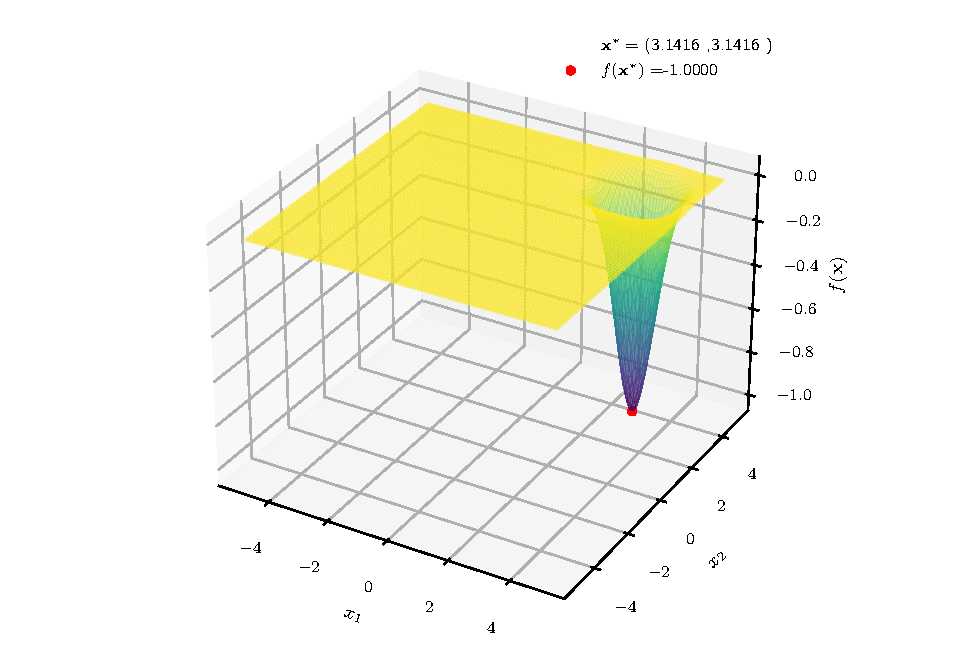
\includegraphics[0.5\textwidth]{easom_optimum.pdf}}
    }
    \subfloat[\path{eggholder}]{%
        \scalebox{.5}{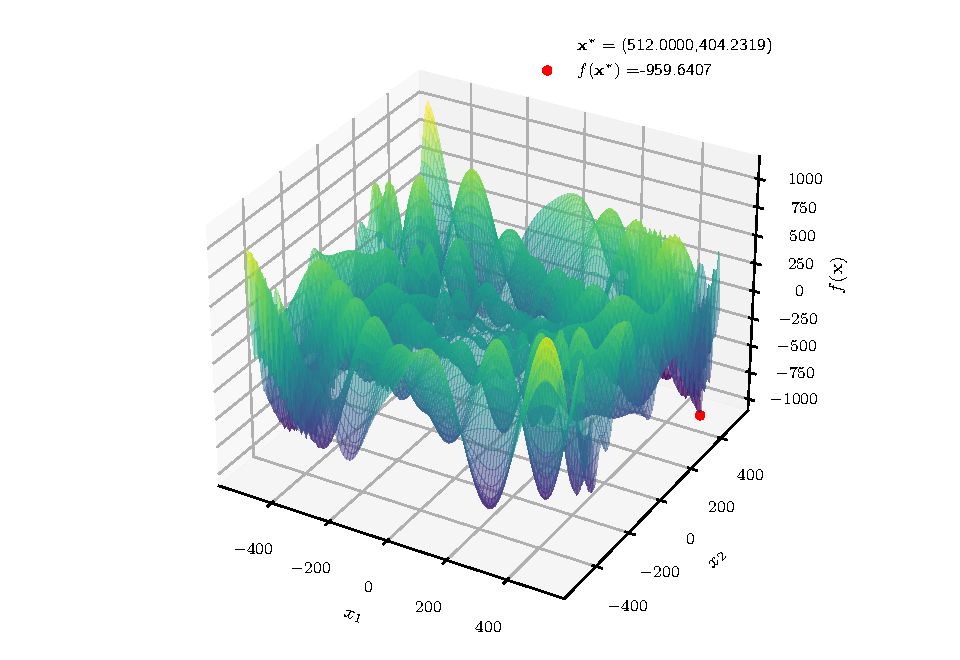
\includegraphics[0.5\textwidth]{eggholder_optimum.pdf}}
    }

    \subfloat[\path{griewank}]{%
        \scalebox{.5}{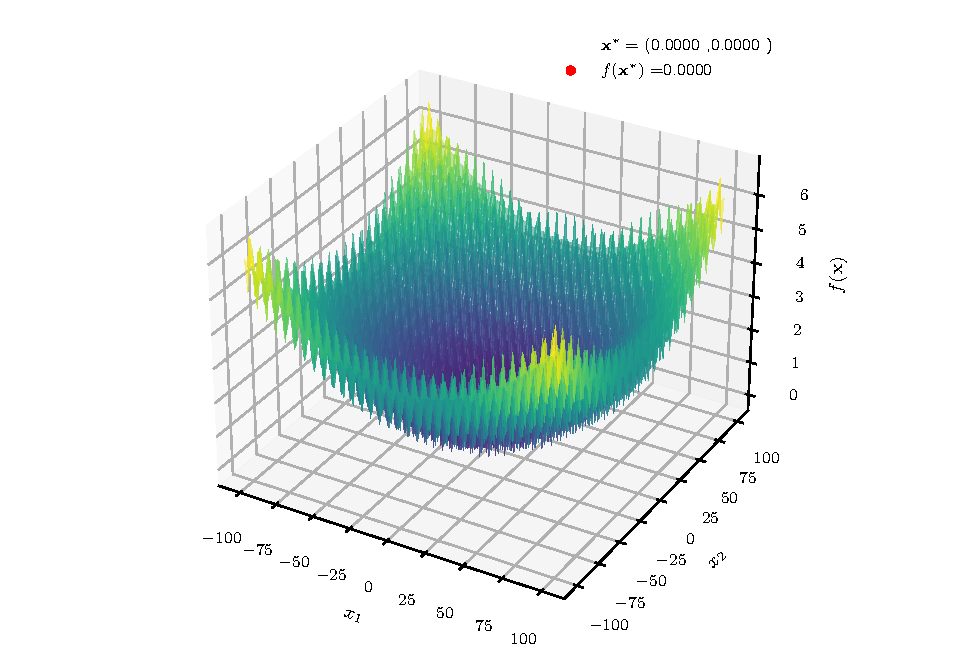
\includegraphics[0.5\textwidth]{griewank_optimum.pdf}}
    }
    \subfloat[\path{shubert}]{%
        \scalebox{.5}{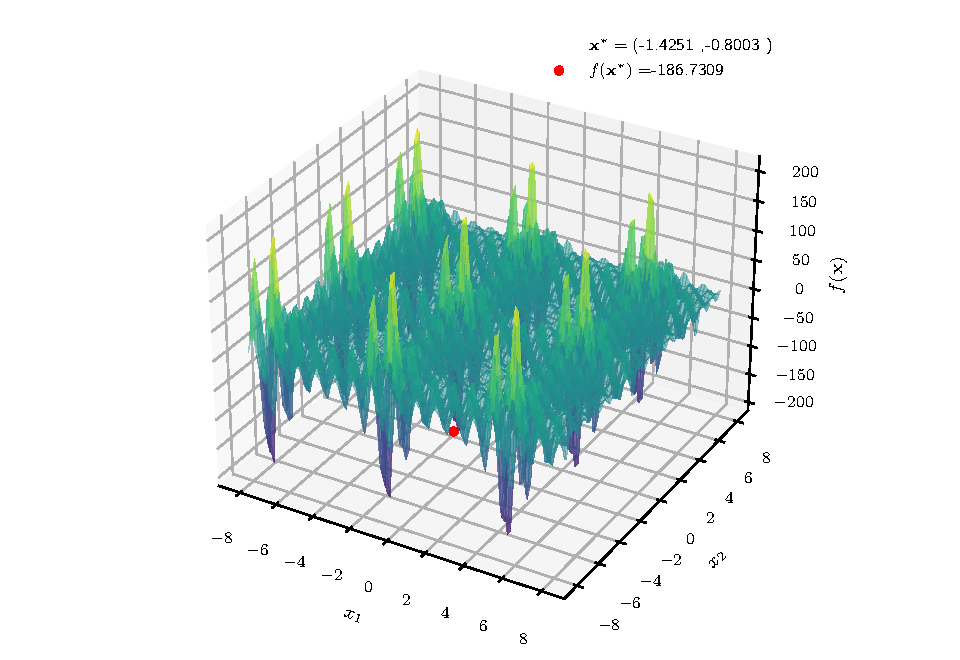
\includegraphics[0.5\textwidth]{shubert_optimum.pdf}}
    }

    \subfloat[\path{sixhump}]{%
        \scalebox{.5}{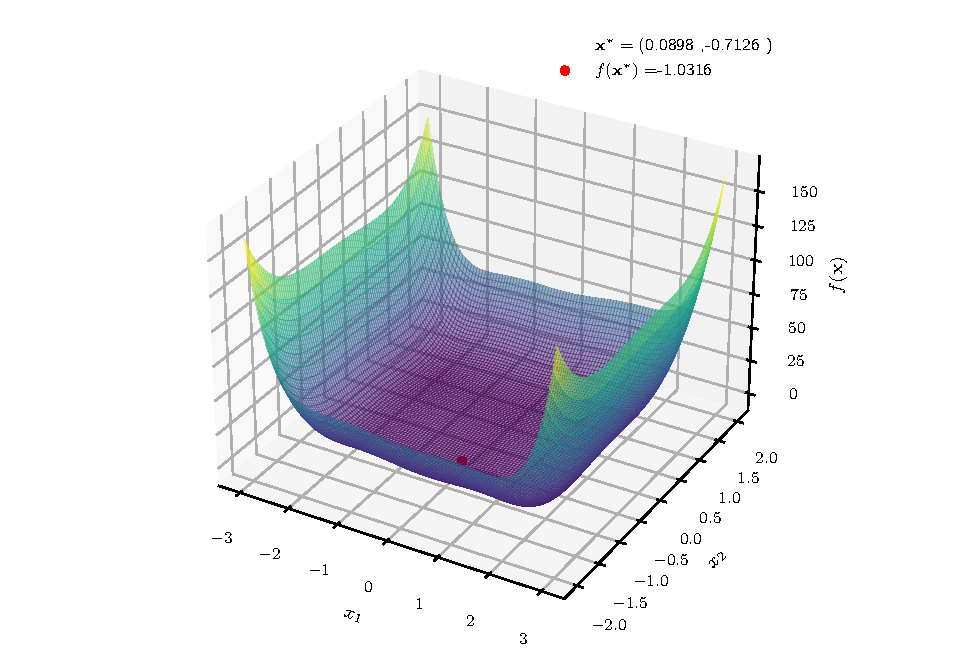
\includegraphics[0.5\textwidth]{sixhump_optimum.pdf}}
    }
    \subfloat[\path{regularized_ts}]{%
        \scalebox{.5}{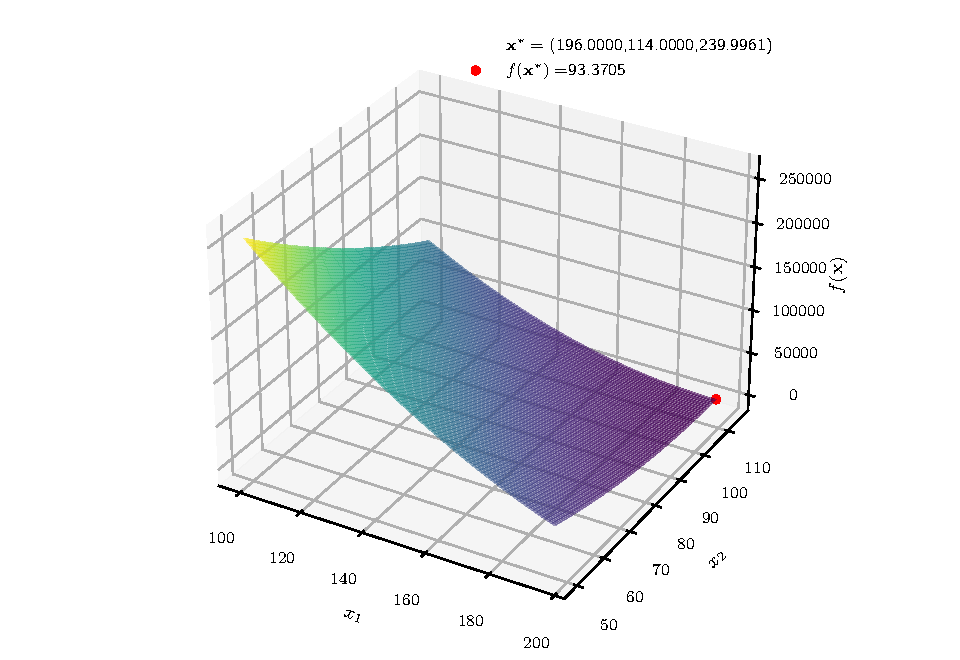
\includegraphics[0.5\textwidth]{regularized_ts_optimum.pdf}}
    }
\end{figure}

\label{sec:analise_estatistica}
\section{Análise Estatística (PSO, FPA, SOS)}

Para manter a isonomia do resultados, todos os algoritmos foram testados 20 vezes para
cada uma das funções objetivo, utilizando sempre uma população com o mesmo número de 
80 indivíduos e uma quantidade máximo de 200 avaliações da função objetivo como critério 
de parada. Os resultados de convergência são apresentados em função do número de iterações. 
No caso da meta heurística \texit{SOS}, cada iteração executa 4 avaliações da função objetivo
e por esse motivo as curvas de convergência possuem um número total de iterações menor que os
demais.

O algoritmo \texit{PSO} requer outros hiper parâmetros além do critério de parada e tamanho da população.
São eles, uma limitação para os vetores de velocidade, escolhido entre \( [-1, 1] \), uma função para
os pesos de inércia, nesse caso foi utilizada uma distribuição randômica, e também coeficientes de aceleração
individuais, fixados em \( c_1=1 \) e \(c_2=1.5 \).

O algoritmo \texit{FPA} requer um parâmetro de peso que controla a permuta entre um processo de
polinização local e um processo global, foi escolhido o valor \( p=0.75 \). O algoritmo \texit{SOS} não requer
outros hiper parâmetros.

As Figura de \ref{fig:statistic_easom} à \ref{fig:statistic_regularized_ts} apresentam na coluna da esquerda
um gráfico de dispersão dos valores mínimos obtividos nas 20 rodadas para cada uma das funções objetivo testadas, e 
na colunda da direita, gráficos de convergência ao longo das iterações mostrando o intervalo de confiância 
de \( 95 \% \) em torno da tendência central.

\begin{figure}[!ht]
    \centering
    \caption{Função objetivo \path{easom}.}
    \label{fig:statistic_easom}
    \subfloat[Dispersão.]{%
        \scalebox{.8}{%% Creator: Matplotlib, PGF backend
%%
%% To include the figure in your LaTeX document, write
%%   \input{<filename>.pgf}
%%
%% Make sure the required packages are loaded in your preamble
%%   \usepackage{pgf}
%%
%% Also ensure that all the required font packages are loaded; for instance,
%% the lmodern package is sometimes necessary when using math font.
%%   \usepackage{lmodern}
%%
%% Figures using additional raster images can only be included by \input if
%% they are in the same directory as the main LaTeX file. For loading figures
%% from other directories you can use the `import` package
%%   \usepackage{import}
%%
%% and then include the figures with
%%   \import{<path to file>}{<filename>.pgf}
%%
%% Matplotlib used the following preamble
%%   
%%   \usepackage{fontspec}
%%   \setmainfont{DejaVuSerif.ttf}[Path=\detokenize{/home/ppiper/miniconda3/lib/python3.9/site-packages/matplotlib/mpl-data/fonts/ttf/}]
%%   \setsansfont{DejaVuSans.ttf}[Path=\detokenize{/home/ppiper/miniconda3/lib/python3.9/site-packages/matplotlib/mpl-data/fonts/ttf/}]
%%   \setmonofont{DejaVuSansMono.ttf}[Path=\detokenize{/home/ppiper/miniconda3/lib/python3.9/site-packages/matplotlib/mpl-data/fonts/ttf/}]
%%   \makeatletter\@ifpackageloaded{underscore}{}{\usepackage[strings]{underscore}}\makeatother
%%
\begingroup%
\makeatletter%
\begin{pgfpicture}%
\pgfpathrectangle{\pgfpointorigin}{\pgfqpoint{4.000000in}{3.000000in}}%
\pgfusepath{use as bounding box, clip}%
\begin{pgfscope}%
\pgfsetbuttcap%
\pgfsetmiterjoin%
\definecolor{currentfill}{rgb}{1.000000,1.000000,1.000000}%
\pgfsetfillcolor{currentfill}%
\pgfsetlinewidth{0.000000pt}%
\definecolor{currentstroke}{rgb}{1.000000,1.000000,1.000000}%
\pgfsetstrokecolor{currentstroke}%
\pgfsetdash{}{0pt}%
\pgfpathmoveto{\pgfqpoint{0.000000in}{0.000000in}}%
\pgfpathlineto{\pgfqpoint{4.000000in}{0.000000in}}%
\pgfpathlineto{\pgfqpoint{4.000000in}{3.000000in}}%
\pgfpathlineto{\pgfqpoint{0.000000in}{3.000000in}}%
\pgfpathlineto{\pgfqpoint{0.000000in}{0.000000in}}%
\pgfpathclose%
\pgfusepath{fill}%
\end{pgfscope}%
\begin{pgfscope}%
\pgfsetbuttcap%
\pgfsetmiterjoin%
\definecolor{currentfill}{rgb}{1.000000,1.000000,1.000000}%
\pgfsetfillcolor{currentfill}%
\pgfsetlinewidth{0.000000pt}%
\definecolor{currentstroke}{rgb}{0.000000,0.000000,0.000000}%
\pgfsetstrokecolor{currentstroke}%
\pgfsetstrokeopacity{0.000000}%
\pgfsetdash{}{0pt}%
\pgfpathmoveto{\pgfqpoint{0.813093in}{0.374785in}}%
\pgfpathlineto{\pgfqpoint{3.850000in}{0.374785in}}%
\pgfpathlineto{\pgfqpoint{3.850000in}{2.850000in}}%
\pgfpathlineto{\pgfqpoint{0.813093in}{2.850000in}}%
\pgfpathlineto{\pgfqpoint{0.813093in}{0.374785in}}%
\pgfpathclose%
\pgfusepath{fill}%
\end{pgfscope}%
\begin{pgfscope}%
\pgfsetbuttcap%
\pgfsetroundjoin%
\definecolor{currentfill}{rgb}{0.000000,0.000000,0.000000}%
\pgfsetfillcolor{currentfill}%
\pgfsetlinewidth{0.803000pt}%
\definecolor{currentstroke}{rgb}{0.000000,0.000000,0.000000}%
\pgfsetstrokecolor{currentstroke}%
\pgfsetdash{}{0pt}%
\pgfsys@defobject{currentmarker}{\pgfqpoint{0.000000in}{-0.048611in}}{\pgfqpoint{0.000000in}{0.000000in}}{%
\pgfpathmoveto{\pgfqpoint{0.000000in}{0.000000in}}%
\pgfpathlineto{\pgfqpoint{0.000000in}{-0.048611in}}%
\pgfusepath{stroke,fill}%
}%
\begin{pgfscope}%
\pgfsys@transformshift{1.319244in}{0.374785in}%
\pgfsys@useobject{currentmarker}{}%
\end{pgfscope}%
\end{pgfscope}%
\begin{pgfscope}%
\definecolor{textcolor}{rgb}{0.000000,0.000000,0.000000}%
\pgfsetstrokecolor{textcolor}%
\pgfsetfillcolor{textcolor}%
\pgftext[x=1.319244in,y=0.248396in,,top]{\color{textcolor}\sffamily\fontsize{8.000000}{9.600000}\selectfont PSO}%
\end{pgfscope}%
\begin{pgfscope}%
\pgfsetbuttcap%
\pgfsetroundjoin%
\definecolor{currentfill}{rgb}{0.000000,0.000000,0.000000}%
\pgfsetfillcolor{currentfill}%
\pgfsetlinewidth{0.803000pt}%
\definecolor{currentstroke}{rgb}{0.000000,0.000000,0.000000}%
\pgfsetstrokecolor{currentstroke}%
\pgfsetdash{}{0pt}%
\pgfsys@defobject{currentmarker}{\pgfqpoint{0.000000in}{-0.048611in}}{\pgfqpoint{0.000000in}{0.000000in}}{%
\pgfpathmoveto{\pgfqpoint{0.000000in}{0.000000in}}%
\pgfpathlineto{\pgfqpoint{0.000000in}{-0.048611in}}%
\pgfusepath{stroke,fill}%
}%
\begin{pgfscope}%
\pgfsys@transformshift{2.331546in}{0.374785in}%
\pgfsys@useobject{currentmarker}{}%
\end{pgfscope}%
\end{pgfscope}%
\begin{pgfscope}%
\definecolor{textcolor}{rgb}{0.000000,0.000000,0.000000}%
\pgfsetstrokecolor{textcolor}%
\pgfsetfillcolor{textcolor}%
\pgftext[x=2.331546in,y=0.248396in,,top]{\color{textcolor}\sffamily\fontsize{8.000000}{9.600000}\selectfont FPA}%
\end{pgfscope}%
\begin{pgfscope}%
\pgfsetbuttcap%
\pgfsetroundjoin%
\definecolor{currentfill}{rgb}{0.000000,0.000000,0.000000}%
\pgfsetfillcolor{currentfill}%
\pgfsetlinewidth{0.803000pt}%
\definecolor{currentstroke}{rgb}{0.000000,0.000000,0.000000}%
\pgfsetstrokecolor{currentstroke}%
\pgfsetdash{}{0pt}%
\pgfsys@defobject{currentmarker}{\pgfqpoint{0.000000in}{-0.048611in}}{\pgfqpoint{0.000000in}{0.000000in}}{%
\pgfpathmoveto{\pgfqpoint{0.000000in}{0.000000in}}%
\pgfpathlineto{\pgfqpoint{0.000000in}{-0.048611in}}%
\pgfusepath{stroke,fill}%
}%
\begin{pgfscope}%
\pgfsys@transformshift{3.343849in}{0.374785in}%
\pgfsys@useobject{currentmarker}{}%
\end{pgfscope}%
\end{pgfscope}%
\begin{pgfscope}%
\definecolor{textcolor}{rgb}{0.000000,0.000000,0.000000}%
\pgfsetstrokecolor{textcolor}%
\pgfsetfillcolor{textcolor}%
\pgftext[x=3.343849in,y=0.248396in,,top]{\color{textcolor}\sffamily\fontsize{8.000000}{9.600000}\selectfont SOS}%
\end{pgfscope}%
\begin{pgfscope}%
\pgfsetbuttcap%
\pgfsetroundjoin%
\definecolor{currentfill}{rgb}{0.000000,0.000000,0.000000}%
\pgfsetfillcolor{currentfill}%
\pgfsetlinewidth{0.803000pt}%
\definecolor{currentstroke}{rgb}{0.000000,0.000000,0.000000}%
\pgfsetstrokecolor{currentstroke}%
\pgfsetdash{}{0pt}%
\pgfsys@defobject{currentmarker}{\pgfqpoint{-0.048611in}{0.000000in}}{\pgfqpoint{-0.000000in}{0.000000in}}{%
\pgfpathmoveto{\pgfqpoint{-0.000000in}{0.000000in}}%
\pgfpathlineto{\pgfqpoint{-0.048611in}{0.000000in}}%
\pgfusepath{stroke,fill}%
}%
\begin{pgfscope}%
\pgfsys@transformshift{0.813093in}{0.487295in}%
\pgfsys@useobject{currentmarker}{}%
\end{pgfscope}%
\end{pgfscope}%
\begin{pgfscope}%
\definecolor{textcolor}{rgb}{0.000000,0.000000,0.000000}%
\pgfsetstrokecolor{textcolor}%
\pgfsetfillcolor{textcolor}%
\pgftext[x=0.325973in, y=0.445086in, left, base]{\color{textcolor}\sffamily\fontsize{8.000000}{9.600000}\selectfont \(\displaystyle {\ensuremath{-}1.000}\)}%
\end{pgfscope}%
\begin{pgfscope}%
\pgfsetbuttcap%
\pgfsetroundjoin%
\definecolor{currentfill}{rgb}{0.000000,0.000000,0.000000}%
\pgfsetfillcolor{currentfill}%
\pgfsetlinewidth{0.803000pt}%
\definecolor{currentstroke}{rgb}{0.000000,0.000000,0.000000}%
\pgfsetstrokecolor{currentstroke}%
\pgfsetdash{}{0pt}%
\pgfsys@defobject{currentmarker}{\pgfqpoint{-0.048611in}{0.000000in}}{\pgfqpoint{-0.000000in}{0.000000in}}{%
\pgfpathmoveto{\pgfqpoint{-0.000000in}{0.000000in}}%
\pgfpathlineto{\pgfqpoint{-0.048611in}{0.000000in}}%
\pgfusepath{stroke,fill}%
}%
\begin{pgfscope}%
\pgfsys@transformshift{0.813093in}{0.817803in}%
\pgfsys@useobject{currentmarker}{}%
\end{pgfscope}%
\end{pgfscope}%
\begin{pgfscope}%
\definecolor{textcolor}{rgb}{0.000000,0.000000,0.000000}%
\pgfsetstrokecolor{textcolor}%
\pgfsetfillcolor{textcolor}%
\pgftext[x=0.325973in, y=0.775594in, left, base]{\color{textcolor}\sffamily\fontsize{8.000000}{9.600000}\selectfont \(\displaystyle {\ensuremath{-}0.999}\)}%
\end{pgfscope}%
\begin{pgfscope}%
\pgfsetbuttcap%
\pgfsetroundjoin%
\definecolor{currentfill}{rgb}{0.000000,0.000000,0.000000}%
\pgfsetfillcolor{currentfill}%
\pgfsetlinewidth{0.803000pt}%
\definecolor{currentstroke}{rgb}{0.000000,0.000000,0.000000}%
\pgfsetstrokecolor{currentstroke}%
\pgfsetdash{}{0pt}%
\pgfsys@defobject{currentmarker}{\pgfqpoint{-0.048611in}{0.000000in}}{\pgfqpoint{-0.000000in}{0.000000in}}{%
\pgfpathmoveto{\pgfqpoint{-0.000000in}{0.000000in}}%
\pgfpathlineto{\pgfqpoint{-0.048611in}{0.000000in}}%
\pgfusepath{stroke,fill}%
}%
\begin{pgfscope}%
\pgfsys@transformshift{0.813093in}{1.148310in}%
\pgfsys@useobject{currentmarker}{}%
\end{pgfscope}%
\end{pgfscope}%
\begin{pgfscope}%
\definecolor{textcolor}{rgb}{0.000000,0.000000,0.000000}%
\pgfsetstrokecolor{textcolor}%
\pgfsetfillcolor{textcolor}%
\pgftext[x=0.325973in, y=1.106101in, left, base]{\color{textcolor}\sffamily\fontsize{8.000000}{9.600000}\selectfont \(\displaystyle {\ensuremath{-}0.998}\)}%
\end{pgfscope}%
\begin{pgfscope}%
\pgfsetbuttcap%
\pgfsetroundjoin%
\definecolor{currentfill}{rgb}{0.000000,0.000000,0.000000}%
\pgfsetfillcolor{currentfill}%
\pgfsetlinewidth{0.803000pt}%
\definecolor{currentstroke}{rgb}{0.000000,0.000000,0.000000}%
\pgfsetstrokecolor{currentstroke}%
\pgfsetdash{}{0pt}%
\pgfsys@defobject{currentmarker}{\pgfqpoint{-0.048611in}{0.000000in}}{\pgfqpoint{-0.000000in}{0.000000in}}{%
\pgfpathmoveto{\pgfqpoint{-0.000000in}{0.000000in}}%
\pgfpathlineto{\pgfqpoint{-0.048611in}{0.000000in}}%
\pgfusepath{stroke,fill}%
}%
\begin{pgfscope}%
\pgfsys@transformshift{0.813093in}{1.478818in}%
\pgfsys@useobject{currentmarker}{}%
\end{pgfscope}%
\end{pgfscope}%
\begin{pgfscope}%
\definecolor{textcolor}{rgb}{0.000000,0.000000,0.000000}%
\pgfsetstrokecolor{textcolor}%
\pgfsetfillcolor{textcolor}%
\pgftext[x=0.325973in, y=1.436609in, left, base]{\color{textcolor}\sffamily\fontsize{8.000000}{9.600000}\selectfont \(\displaystyle {\ensuremath{-}0.997}\)}%
\end{pgfscope}%
\begin{pgfscope}%
\pgfsetbuttcap%
\pgfsetroundjoin%
\definecolor{currentfill}{rgb}{0.000000,0.000000,0.000000}%
\pgfsetfillcolor{currentfill}%
\pgfsetlinewidth{0.803000pt}%
\definecolor{currentstroke}{rgb}{0.000000,0.000000,0.000000}%
\pgfsetstrokecolor{currentstroke}%
\pgfsetdash{}{0pt}%
\pgfsys@defobject{currentmarker}{\pgfqpoint{-0.048611in}{0.000000in}}{\pgfqpoint{-0.000000in}{0.000000in}}{%
\pgfpathmoveto{\pgfqpoint{-0.000000in}{0.000000in}}%
\pgfpathlineto{\pgfqpoint{-0.048611in}{0.000000in}}%
\pgfusepath{stroke,fill}%
}%
\begin{pgfscope}%
\pgfsys@transformshift{0.813093in}{1.809326in}%
\pgfsys@useobject{currentmarker}{}%
\end{pgfscope}%
\end{pgfscope}%
\begin{pgfscope}%
\definecolor{textcolor}{rgb}{0.000000,0.000000,0.000000}%
\pgfsetstrokecolor{textcolor}%
\pgfsetfillcolor{textcolor}%
\pgftext[x=0.325973in, y=1.767116in, left, base]{\color{textcolor}\sffamily\fontsize{8.000000}{9.600000}\selectfont \(\displaystyle {\ensuremath{-}0.996}\)}%
\end{pgfscope}%
\begin{pgfscope}%
\pgfsetbuttcap%
\pgfsetroundjoin%
\definecolor{currentfill}{rgb}{0.000000,0.000000,0.000000}%
\pgfsetfillcolor{currentfill}%
\pgfsetlinewidth{0.803000pt}%
\definecolor{currentstroke}{rgb}{0.000000,0.000000,0.000000}%
\pgfsetstrokecolor{currentstroke}%
\pgfsetdash{}{0pt}%
\pgfsys@defobject{currentmarker}{\pgfqpoint{-0.048611in}{0.000000in}}{\pgfqpoint{-0.000000in}{0.000000in}}{%
\pgfpathmoveto{\pgfqpoint{-0.000000in}{0.000000in}}%
\pgfpathlineto{\pgfqpoint{-0.048611in}{0.000000in}}%
\pgfusepath{stroke,fill}%
}%
\begin{pgfscope}%
\pgfsys@transformshift{0.813093in}{2.139833in}%
\pgfsys@useobject{currentmarker}{}%
\end{pgfscope}%
\end{pgfscope}%
\begin{pgfscope}%
\definecolor{textcolor}{rgb}{0.000000,0.000000,0.000000}%
\pgfsetstrokecolor{textcolor}%
\pgfsetfillcolor{textcolor}%
\pgftext[x=0.325973in, y=2.097624in, left, base]{\color{textcolor}\sffamily\fontsize{8.000000}{9.600000}\selectfont \(\displaystyle {\ensuremath{-}0.995}\)}%
\end{pgfscope}%
\begin{pgfscope}%
\pgfsetbuttcap%
\pgfsetroundjoin%
\definecolor{currentfill}{rgb}{0.000000,0.000000,0.000000}%
\pgfsetfillcolor{currentfill}%
\pgfsetlinewidth{0.803000pt}%
\definecolor{currentstroke}{rgb}{0.000000,0.000000,0.000000}%
\pgfsetstrokecolor{currentstroke}%
\pgfsetdash{}{0pt}%
\pgfsys@defobject{currentmarker}{\pgfqpoint{-0.048611in}{0.000000in}}{\pgfqpoint{-0.000000in}{0.000000in}}{%
\pgfpathmoveto{\pgfqpoint{-0.000000in}{0.000000in}}%
\pgfpathlineto{\pgfqpoint{-0.048611in}{0.000000in}}%
\pgfusepath{stroke,fill}%
}%
\begin{pgfscope}%
\pgfsys@transformshift{0.813093in}{2.470341in}%
\pgfsys@useobject{currentmarker}{}%
\end{pgfscope}%
\end{pgfscope}%
\begin{pgfscope}%
\definecolor{textcolor}{rgb}{0.000000,0.000000,0.000000}%
\pgfsetstrokecolor{textcolor}%
\pgfsetfillcolor{textcolor}%
\pgftext[x=0.325973in, y=2.428132in, left, base]{\color{textcolor}\sffamily\fontsize{8.000000}{9.600000}\selectfont \(\displaystyle {\ensuremath{-}0.994}\)}%
\end{pgfscope}%
\begin{pgfscope}%
\pgfsetbuttcap%
\pgfsetroundjoin%
\definecolor{currentfill}{rgb}{0.000000,0.000000,0.000000}%
\pgfsetfillcolor{currentfill}%
\pgfsetlinewidth{0.803000pt}%
\definecolor{currentstroke}{rgb}{0.000000,0.000000,0.000000}%
\pgfsetstrokecolor{currentstroke}%
\pgfsetdash{}{0pt}%
\pgfsys@defobject{currentmarker}{\pgfqpoint{-0.048611in}{0.000000in}}{\pgfqpoint{-0.000000in}{0.000000in}}{%
\pgfpathmoveto{\pgfqpoint{-0.000000in}{0.000000in}}%
\pgfpathlineto{\pgfqpoint{-0.048611in}{0.000000in}}%
\pgfusepath{stroke,fill}%
}%
\begin{pgfscope}%
\pgfsys@transformshift{0.813093in}{2.800849in}%
\pgfsys@useobject{currentmarker}{}%
\end{pgfscope}%
\end{pgfscope}%
\begin{pgfscope}%
\definecolor{textcolor}{rgb}{0.000000,0.000000,0.000000}%
\pgfsetstrokecolor{textcolor}%
\pgfsetfillcolor{textcolor}%
\pgftext[x=0.325973in, y=2.758639in, left, base]{\color{textcolor}\sffamily\fontsize{8.000000}{9.600000}\selectfont \(\displaystyle {\ensuremath{-}0.993}\)}%
\end{pgfscope}%
\begin{pgfscope}%
\definecolor{textcolor}{rgb}{0.000000,0.000000,0.000000}%
\pgfsetstrokecolor{textcolor}%
\pgfsetfillcolor{textcolor}%
\pgftext[x=0.270418in,y=1.612393in,,bottom,rotate=90.000000]{\color{textcolor}\sffamily\fontsize{8.800000}{10.560000}\selectfont \(\displaystyle f(\mathbf{x}^*)\)}%
\end{pgfscope}%
\begin{pgfscope}%
\pgfpathrectangle{\pgfqpoint{0.813093in}{0.374785in}}{\pgfqpoint{3.036907in}{2.475215in}}%
\pgfusepath{clip}%
\pgfsetrectcap%
\pgfsetroundjoin%
\pgfsetlinewidth{1.003750pt}%
\definecolor{currentstroke}{rgb}{0.000000,0.000000,0.000000}%
\pgfsetstrokecolor{currentstroke}%
\pgfsetdash{}{0pt}%
\pgfpathmoveto{\pgfqpoint{1.167399in}{0.487295in}}%
\pgfpathlineto{\pgfqpoint{1.471089in}{0.487295in}}%
\pgfpathlineto{\pgfqpoint{1.471089in}{0.487295in}}%
\pgfpathlineto{\pgfqpoint{1.167399in}{0.487295in}}%
\pgfpathlineto{\pgfqpoint{1.167399in}{0.487295in}}%
\pgfusepath{stroke}%
\end{pgfscope}%
\begin{pgfscope}%
\pgfpathrectangle{\pgfqpoint{0.813093in}{0.374785in}}{\pgfqpoint{3.036907in}{2.475215in}}%
\pgfusepath{clip}%
\pgfsetrectcap%
\pgfsetroundjoin%
\pgfsetlinewidth{1.003750pt}%
\definecolor{currentstroke}{rgb}{0.000000,0.000000,0.000000}%
\pgfsetstrokecolor{currentstroke}%
\pgfsetdash{}{0pt}%
\pgfpathmoveto{\pgfqpoint{1.319244in}{0.487295in}}%
\pgfpathlineto{\pgfqpoint{1.319244in}{0.487295in}}%
\pgfusepath{stroke}%
\end{pgfscope}%
\begin{pgfscope}%
\pgfpathrectangle{\pgfqpoint{0.813093in}{0.374785in}}{\pgfqpoint{3.036907in}{2.475215in}}%
\pgfusepath{clip}%
\pgfsetrectcap%
\pgfsetroundjoin%
\pgfsetlinewidth{1.003750pt}%
\definecolor{currentstroke}{rgb}{0.000000,0.000000,0.000000}%
\pgfsetstrokecolor{currentstroke}%
\pgfsetdash{}{0pt}%
\pgfpathmoveto{\pgfqpoint{1.319244in}{0.487295in}}%
\pgfpathlineto{\pgfqpoint{1.319244in}{0.487295in}}%
\pgfusepath{stroke}%
\end{pgfscope}%
\begin{pgfscope}%
\pgfpathrectangle{\pgfqpoint{0.813093in}{0.374785in}}{\pgfqpoint{3.036907in}{2.475215in}}%
\pgfusepath{clip}%
\pgfsetrectcap%
\pgfsetroundjoin%
\pgfsetlinewidth{1.003750pt}%
\definecolor{currentstroke}{rgb}{0.000000,0.000000,0.000000}%
\pgfsetstrokecolor{currentstroke}%
\pgfsetdash{}{0pt}%
\pgfpathmoveto{\pgfqpoint{1.243321in}{0.487295in}}%
\pgfpathlineto{\pgfqpoint{1.395167in}{0.487295in}}%
\pgfusepath{stroke}%
\end{pgfscope}%
\begin{pgfscope}%
\pgfpathrectangle{\pgfqpoint{0.813093in}{0.374785in}}{\pgfqpoint{3.036907in}{2.475215in}}%
\pgfusepath{clip}%
\pgfsetrectcap%
\pgfsetroundjoin%
\pgfsetlinewidth{1.003750pt}%
\definecolor{currentstroke}{rgb}{0.000000,0.000000,0.000000}%
\pgfsetstrokecolor{currentstroke}%
\pgfsetdash{}{0pt}%
\pgfpathmoveto{\pgfqpoint{1.243321in}{0.487295in}}%
\pgfpathlineto{\pgfqpoint{1.395167in}{0.487295in}}%
\pgfusepath{stroke}%
\end{pgfscope}%
\begin{pgfscope}%
\pgfpathrectangle{\pgfqpoint{0.813093in}{0.374785in}}{\pgfqpoint{3.036907in}{2.475215in}}%
\pgfusepath{clip}%
\pgfsetrectcap%
\pgfsetroundjoin%
\pgfsetlinewidth{1.003750pt}%
\definecolor{currentstroke}{rgb}{0.000000,0.000000,0.000000}%
\pgfsetstrokecolor{currentstroke}%
\pgfsetdash{}{0pt}%
\pgfpathmoveto{\pgfqpoint{2.179701in}{0.744796in}}%
\pgfpathlineto{\pgfqpoint{2.483392in}{0.744796in}}%
\pgfpathlineto{\pgfqpoint{2.483392in}{1.376369in}}%
\pgfpathlineto{\pgfqpoint{2.179701in}{1.376369in}}%
\pgfpathlineto{\pgfqpoint{2.179701in}{0.744796in}}%
\pgfusepath{stroke}%
\end{pgfscope}%
\begin{pgfscope}%
\pgfpathrectangle{\pgfqpoint{0.813093in}{0.374785in}}{\pgfqpoint{3.036907in}{2.475215in}}%
\pgfusepath{clip}%
\pgfsetrectcap%
\pgfsetroundjoin%
\pgfsetlinewidth{1.003750pt}%
\definecolor{currentstroke}{rgb}{0.000000,0.000000,0.000000}%
\pgfsetstrokecolor{currentstroke}%
\pgfsetdash{}{0pt}%
\pgfpathmoveto{\pgfqpoint{2.331546in}{0.744796in}}%
\pgfpathlineto{\pgfqpoint{2.331546in}{0.487394in}}%
\pgfusepath{stroke}%
\end{pgfscope}%
\begin{pgfscope}%
\pgfpathrectangle{\pgfqpoint{0.813093in}{0.374785in}}{\pgfqpoint{3.036907in}{2.475215in}}%
\pgfusepath{clip}%
\pgfsetrectcap%
\pgfsetroundjoin%
\pgfsetlinewidth{1.003750pt}%
\definecolor{currentstroke}{rgb}{0.000000,0.000000,0.000000}%
\pgfsetstrokecolor{currentstroke}%
\pgfsetdash{}{0pt}%
\pgfpathmoveto{\pgfqpoint{2.331546in}{1.376369in}}%
\pgfpathlineto{\pgfqpoint{2.331546in}{2.163666in}}%
\pgfusepath{stroke}%
\end{pgfscope}%
\begin{pgfscope}%
\pgfpathrectangle{\pgfqpoint{0.813093in}{0.374785in}}{\pgfqpoint{3.036907in}{2.475215in}}%
\pgfusepath{clip}%
\pgfsetrectcap%
\pgfsetroundjoin%
\pgfsetlinewidth{1.003750pt}%
\definecolor{currentstroke}{rgb}{0.000000,0.000000,0.000000}%
\pgfsetstrokecolor{currentstroke}%
\pgfsetdash{}{0pt}%
\pgfpathmoveto{\pgfqpoint{2.255624in}{0.487394in}}%
\pgfpathlineto{\pgfqpoint{2.407469in}{0.487394in}}%
\pgfusepath{stroke}%
\end{pgfscope}%
\begin{pgfscope}%
\pgfpathrectangle{\pgfqpoint{0.813093in}{0.374785in}}{\pgfqpoint{3.036907in}{2.475215in}}%
\pgfusepath{clip}%
\pgfsetrectcap%
\pgfsetroundjoin%
\pgfsetlinewidth{1.003750pt}%
\definecolor{currentstroke}{rgb}{0.000000,0.000000,0.000000}%
\pgfsetstrokecolor{currentstroke}%
\pgfsetdash{}{0pt}%
\pgfpathmoveto{\pgfqpoint{2.255624in}{2.163666in}}%
\pgfpathlineto{\pgfqpoint{2.407469in}{2.163666in}}%
\pgfusepath{stroke}%
\end{pgfscope}%
\begin{pgfscope}%
\pgfpathrectangle{\pgfqpoint{0.813093in}{0.374785in}}{\pgfqpoint{3.036907in}{2.475215in}}%
\pgfusepath{clip}%
\pgfsetbuttcap%
\pgfsetroundjoin%
\definecolor{currentfill}{rgb}{0.000000,0.000000,0.000000}%
\pgfsetfillcolor{currentfill}%
\pgfsetfillopacity{0.000000}%
\pgfsetlinewidth{1.003750pt}%
\definecolor{currentstroke}{rgb}{0.000000,0.000000,0.000000}%
\pgfsetstrokecolor{currentstroke}%
\pgfsetdash{}{0pt}%
\pgfsys@defobject{currentmarker}{\pgfqpoint{-0.041667in}{-0.041667in}}{\pgfqpoint{0.041667in}{0.041667in}}{%
\pgfpathmoveto{\pgfqpoint{0.000000in}{-0.041667in}}%
\pgfpathcurveto{\pgfqpoint{0.011050in}{-0.041667in}}{\pgfqpoint{0.021649in}{-0.037276in}}{\pgfqpoint{0.029463in}{-0.029463in}}%
\pgfpathcurveto{\pgfqpoint{0.037276in}{-0.021649in}}{\pgfqpoint{0.041667in}{-0.011050in}}{\pgfqpoint{0.041667in}{0.000000in}}%
\pgfpathcurveto{\pgfqpoint{0.041667in}{0.011050in}}{\pgfqpoint{0.037276in}{0.021649in}}{\pgfqpoint{0.029463in}{0.029463in}}%
\pgfpathcurveto{\pgfqpoint{0.021649in}{0.037276in}}{\pgfqpoint{0.011050in}{0.041667in}}{\pgfqpoint{0.000000in}{0.041667in}}%
\pgfpathcurveto{\pgfqpoint{-0.011050in}{0.041667in}}{\pgfqpoint{-0.021649in}{0.037276in}}{\pgfqpoint{-0.029463in}{0.029463in}}%
\pgfpathcurveto{\pgfqpoint{-0.037276in}{0.021649in}}{\pgfqpoint{-0.041667in}{0.011050in}}{\pgfqpoint{-0.041667in}{0.000000in}}%
\pgfpathcurveto{\pgfqpoint{-0.041667in}{-0.011050in}}{\pgfqpoint{-0.037276in}{-0.021649in}}{\pgfqpoint{-0.029463in}{-0.029463in}}%
\pgfpathcurveto{\pgfqpoint{-0.021649in}{-0.037276in}}{\pgfqpoint{-0.011050in}{-0.041667in}}{\pgfqpoint{0.000000in}{-0.041667in}}%
\pgfpathlineto{\pgfqpoint{0.000000in}{-0.041667in}}%
\pgfpathclose%
\pgfusepath{stroke,fill}%
}%
\begin{pgfscope}%
\pgfsys@transformshift{2.331546in}{2.737490in}%
\pgfsys@useobject{currentmarker}{}%
\end{pgfscope}%
\begin{pgfscope}%
\pgfsys@transformshift{2.331546in}{2.610124in}%
\pgfsys@useobject{currentmarker}{}%
\end{pgfscope}%
\end{pgfscope}%
\begin{pgfscope}%
\pgfpathrectangle{\pgfqpoint{0.813093in}{0.374785in}}{\pgfqpoint{3.036907in}{2.475215in}}%
\pgfusepath{clip}%
\pgfsetrectcap%
\pgfsetroundjoin%
\pgfsetlinewidth{1.003750pt}%
\definecolor{currentstroke}{rgb}{0.000000,0.000000,0.000000}%
\pgfsetstrokecolor{currentstroke}%
\pgfsetdash{}{0pt}%
\pgfpathmoveto{\pgfqpoint{3.192003in}{0.487295in}}%
\pgfpathlineto{\pgfqpoint{3.495694in}{0.487295in}}%
\pgfpathlineto{\pgfqpoint{3.495694in}{0.487295in}}%
\pgfpathlineto{\pgfqpoint{3.192003in}{0.487295in}}%
\pgfpathlineto{\pgfqpoint{3.192003in}{0.487295in}}%
\pgfusepath{stroke}%
\end{pgfscope}%
\begin{pgfscope}%
\pgfpathrectangle{\pgfqpoint{0.813093in}{0.374785in}}{\pgfqpoint{3.036907in}{2.475215in}}%
\pgfusepath{clip}%
\pgfsetrectcap%
\pgfsetroundjoin%
\pgfsetlinewidth{1.003750pt}%
\definecolor{currentstroke}{rgb}{0.000000,0.000000,0.000000}%
\pgfsetstrokecolor{currentstroke}%
\pgfsetdash{}{0pt}%
\pgfpathmoveto{\pgfqpoint{3.343849in}{0.487295in}}%
\pgfpathlineto{\pgfqpoint{3.343849in}{0.487295in}}%
\pgfusepath{stroke}%
\end{pgfscope}%
\begin{pgfscope}%
\pgfpathrectangle{\pgfqpoint{0.813093in}{0.374785in}}{\pgfqpoint{3.036907in}{2.475215in}}%
\pgfusepath{clip}%
\pgfsetrectcap%
\pgfsetroundjoin%
\pgfsetlinewidth{1.003750pt}%
\definecolor{currentstroke}{rgb}{0.000000,0.000000,0.000000}%
\pgfsetstrokecolor{currentstroke}%
\pgfsetdash{}{0pt}%
\pgfpathmoveto{\pgfqpoint{3.343849in}{0.487295in}}%
\pgfpathlineto{\pgfqpoint{3.343849in}{0.487295in}}%
\pgfusepath{stroke}%
\end{pgfscope}%
\begin{pgfscope}%
\pgfpathrectangle{\pgfqpoint{0.813093in}{0.374785in}}{\pgfqpoint{3.036907in}{2.475215in}}%
\pgfusepath{clip}%
\pgfsetrectcap%
\pgfsetroundjoin%
\pgfsetlinewidth{1.003750pt}%
\definecolor{currentstroke}{rgb}{0.000000,0.000000,0.000000}%
\pgfsetstrokecolor{currentstroke}%
\pgfsetdash{}{0pt}%
\pgfpathmoveto{\pgfqpoint{3.267926in}{0.487295in}}%
\pgfpathlineto{\pgfqpoint{3.419771in}{0.487295in}}%
\pgfusepath{stroke}%
\end{pgfscope}%
\begin{pgfscope}%
\pgfpathrectangle{\pgfqpoint{0.813093in}{0.374785in}}{\pgfqpoint{3.036907in}{2.475215in}}%
\pgfusepath{clip}%
\pgfsetrectcap%
\pgfsetroundjoin%
\pgfsetlinewidth{1.003750pt}%
\definecolor{currentstroke}{rgb}{0.000000,0.000000,0.000000}%
\pgfsetstrokecolor{currentstroke}%
\pgfsetdash{}{0pt}%
\pgfpathmoveto{\pgfqpoint{3.267926in}{0.487295in}}%
\pgfpathlineto{\pgfqpoint{3.419771in}{0.487295in}}%
\pgfusepath{stroke}%
\end{pgfscope}%
\begin{pgfscope}%
\pgfpathrectangle{\pgfqpoint{0.813093in}{0.374785in}}{\pgfqpoint{3.036907in}{2.475215in}}%
\pgfusepath{clip}%
\pgfsetrectcap%
\pgfsetroundjoin%
\pgfsetlinewidth{1.003750pt}%
\definecolor{currentstroke}{rgb}{1.000000,0.498039,0.054902}%
\pgfsetstrokecolor{currentstroke}%
\pgfsetdash{}{0pt}%
\pgfpathmoveto{\pgfqpoint{1.167399in}{0.487295in}}%
\pgfpathlineto{\pgfqpoint{1.471089in}{0.487295in}}%
\pgfusepath{stroke}%
\end{pgfscope}%
\begin{pgfscope}%
\pgfpathrectangle{\pgfqpoint{0.813093in}{0.374785in}}{\pgfqpoint{3.036907in}{2.475215in}}%
\pgfusepath{clip}%
\pgfsetrectcap%
\pgfsetroundjoin%
\pgfsetlinewidth{1.003750pt}%
\definecolor{currentstroke}{rgb}{1.000000,0.498039,0.054902}%
\pgfsetstrokecolor{currentstroke}%
\pgfsetdash{}{0pt}%
\pgfpathmoveto{\pgfqpoint{2.179701in}{1.044342in}}%
\pgfpathlineto{\pgfqpoint{2.483392in}{1.044342in}}%
\pgfusepath{stroke}%
\end{pgfscope}%
\begin{pgfscope}%
\pgfpathrectangle{\pgfqpoint{0.813093in}{0.374785in}}{\pgfqpoint{3.036907in}{2.475215in}}%
\pgfusepath{clip}%
\pgfsetrectcap%
\pgfsetroundjoin%
\pgfsetlinewidth{1.003750pt}%
\definecolor{currentstroke}{rgb}{1.000000,0.498039,0.054902}%
\pgfsetstrokecolor{currentstroke}%
\pgfsetdash{}{0pt}%
\pgfpathmoveto{\pgfqpoint{3.192003in}{0.487295in}}%
\pgfpathlineto{\pgfqpoint{3.495694in}{0.487295in}}%
\pgfusepath{stroke}%
\end{pgfscope}%
\begin{pgfscope}%
\pgfsetrectcap%
\pgfsetmiterjoin%
\pgfsetlinewidth{0.803000pt}%
\definecolor{currentstroke}{rgb}{0.000000,0.000000,0.000000}%
\pgfsetstrokecolor{currentstroke}%
\pgfsetdash{}{0pt}%
\pgfpathmoveto{\pgfqpoint{0.813093in}{0.374785in}}%
\pgfpathlineto{\pgfqpoint{0.813093in}{2.850000in}}%
\pgfusepath{stroke}%
\end{pgfscope}%
\begin{pgfscope}%
\pgfsetrectcap%
\pgfsetmiterjoin%
\pgfsetlinewidth{0.803000pt}%
\definecolor{currentstroke}{rgb}{0.000000,0.000000,0.000000}%
\pgfsetstrokecolor{currentstroke}%
\pgfsetdash{}{0pt}%
\pgfpathmoveto{\pgfqpoint{3.850000in}{0.374785in}}%
\pgfpathlineto{\pgfqpoint{3.850000in}{2.850000in}}%
\pgfusepath{stroke}%
\end{pgfscope}%
\begin{pgfscope}%
\pgfsetrectcap%
\pgfsetmiterjoin%
\pgfsetlinewidth{0.803000pt}%
\definecolor{currentstroke}{rgb}{0.000000,0.000000,0.000000}%
\pgfsetstrokecolor{currentstroke}%
\pgfsetdash{}{0pt}%
\pgfpathmoveto{\pgfqpoint{0.813093in}{0.374785in}}%
\pgfpathlineto{\pgfqpoint{3.850000in}{0.374785in}}%
\pgfusepath{stroke}%
\end{pgfscope}%
\begin{pgfscope}%
\pgfsetrectcap%
\pgfsetmiterjoin%
\pgfsetlinewidth{0.803000pt}%
\definecolor{currentstroke}{rgb}{0.000000,0.000000,0.000000}%
\pgfsetstrokecolor{currentstroke}%
\pgfsetdash{}{0pt}%
\pgfpathmoveto{\pgfqpoint{0.813093in}{2.850000in}}%
\pgfpathlineto{\pgfqpoint{3.850000in}{2.850000in}}%
\pgfusepath{stroke}%
\end{pgfscope}%
\end{pgfpicture}%
\makeatother%
\endgroup%
}
    }
    \subfloat[Convergência.]{%
        \scalebox{.8}{%% Creator: Matplotlib, PGF backend
%%
%% To include the figure in your LaTeX document, write
%%   \input{<filename>.pgf}
%%
%% Make sure the required packages are loaded in your preamble
%%   \usepackage{pgf}
%%
%% Also ensure that all the required font packages are loaded; for instance,
%% the lmodern package is sometimes necessary when using math font.
%%   \usepackage{lmodern}
%%
%% Figures using additional raster images can only be included by \input if
%% they are in the same directory as the main LaTeX file. For loading figures
%% from other directories you can use the `import` package
%%   \usepackage{import}
%%
%% and then include the figures with
%%   \import{<path to file>}{<filename>.pgf}
%%
%% Matplotlib used the following preamble
%%   
%%   \usepackage{fontspec}
%%   \setmainfont{DejaVuSerif.ttf}[Path=\detokenize{/home/ppiper/miniconda3/envs/ene300/lib/python3.11/site-packages/matplotlib/mpl-data/fonts/ttf/}]
%%   \setsansfont{DejaVuSans.ttf}[Path=\detokenize{/home/ppiper/miniconda3/envs/ene300/lib/python3.11/site-packages/matplotlib/mpl-data/fonts/ttf/}]
%%   \setmonofont{DejaVuSansMono.ttf}[Path=\detokenize{/home/ppiper/miniconda3/envs/ene300/lib/python3.11/site-packages/matplotlib/mpl-data/fonts/ttf/}]
%%   \makeatletter\@ifpackageloaded{underscore}{}{\usepackage[strings]{underscore}}\makeatother
%%
\begingroup%
\makeatletter%
\begin{pgfpicture}%
\pgfpathrectangle{\pgfpointorigin}{\pgfqpoint{4.000000in}{3.000000in}}%
\pgfusepath{use as bounding box, clip}%
\begin{pgfscope}%
\pgfsetbuttcap%
\pgfsetmiterjoin%
\definecolor{currentfill}{rgb}{1.000000,1.000000,1.000000}%
\pgfsetfillcolor{currentfill}%
\pgfsetlinewidth{0.000000pt}%
\definecolor{currentstroke}{rgb}{1.000000,1.000000,1.000000}%
\pgfsetstrokecolor{currentstroke}%
\pgfsetdash{}{0pt}%
\pgfpathmoveto{\pgfqpoint{0.000000in}{0.000000in}}%
\pgfpathlineto{\pgfqpoint{4.000000in}{0.000000in}}%
\pgfpathlineto{\pgfqpoint{4.000000in}{3.000000in}}%
\pgfpathlineto{\pgfqpoint{0.000000in}{3.000000in}}%
\pgfpathlineto{\pgfqpoint{0.000000in}{0.000000in}}%
\pgfpathclose%
\pgfusepath{fill}%
\end{pgfscope}%
\begin{pgfscope}%
\pgfsetbuttcap%
\pgfsetmiterjoin%
\definecolor{currentfill}{rgb}{1.000000,1.000000,1.000000}%
\pgfsetfillcolor{currentfill}%
\pgfsetlinewidth{0.000000pt}%
\definecolor{currentstroke}{rgb}{0.000000,0.000000,0.000000}%
\pgfsetstrokecolor{currentstroke}%
\pgfsetstrokeopacity{0.000000}%
\pgfsetdash{}{0pt}%
\pgfpathmoveto{\pgfqpoint{0.760819in}{0.538577in}}%
\pgfpathlineto{\pgfqpoint{3.850000in}{0.538577in}}%
\pgfpathlineto{\pgfqpoint{3.850000in}{2.838369in}}%
\pgfpathlineto{\pgfqpoint{0.760819in}{2.838369in}}%
\pgfpathlineto{\pgfqpoint{0.760819in}{0.538577in}}%
\pgfpathclose%
\pgfusepath{fill}%
\end{pgfscope}%
\begin{pgfscope}%
\pgfpathrectangle{\pgfqpoint{0.760819in}{0.538577in}}{\pgfqpoint{3.089181in}{2.299792in}}%
\pgfusepath{clip}%
\pgfsetbuttcap%
\pgfsetroundjoin%
\definecolor{currentfill}{rgb}{0.121569,0.466667,0.705882}%
\pgfsetfillcolor{currentfill}%
\pgfsetfillopacity{0.200000}%
\pgfsetlinewidth{0.240900pt}%
\definecolor{currentstroke}{rgb}{0.121569,0.466667,0.705882}%
\pgfsetstrokecolor{currentstroke}%
\pgfsetstrokeopacity{0.200000}%
\pgfsetdash{}{0pt}%
\pgfsys@defobject{currentmarker}{\pgfqpoint{0.901236in}{0.643113in}}{\pgfqpoint{3.695470in}{1.607737in}}{%
\pgfpathmoveto{\pgfqpoint{0.901236in}{1.607737in}}%
\pgfpathlineto{\pgfqpoint{0.901236in}{0.960380in}}%
\pgfpathlineto{\pgfqpoint{0.915348in}{0.785294in}}%
\pgfpathlineto{\pgfqpoint{0.929461in}{0.704301in}}%
\pgfpathlineto{\pgfqpoint{0.943573in}{0.677505in}}%
\pgfpathlineto{\pgfqpoint{0.957685in}{0.668659in}}%
\pgfpathlineto{\pgfqpoint{0.971798in}{0.660085in}}%
\pgfpathlineto{\pgfqpoint{0.985910in}{0.654305in}}%
\pgfpathlineto{\pgfqpoint{1.000022in}{0.647616in}}%
\pgfpathlineto{\pgfqpoint{1.014134in}{0.646404in}}%
\pgfpathlineto{\pgfqpoint{1.028247in}{0.645074in}}%
\pgfpathlineto{\pgfqpoint{1.042359in}{0.644894in}}%
\pgfpathlineto{\pgfqpoint{1.056471in}{0.644576in}}%
\pgfpathlineto{\pgfqpoint{1.070584in}{0.644372in}}%
\pgfpathlineto{\pgfqpoint{1.084696in}{0.644046in}}%
\pgfpathlineto{\pgfqpoint{1.098808in}{0.643763in}}%
\pgfpathlineto{\pgfqpoint{1.112921in}{0.643681in}}%
\pgfpathlineto{\pgfqpoint{1.127033in}{0.643504in}}%
\pgfpathlineto{\pgfqpoint{1.141145in}{0.643365in}}%
\pgfpathlineto{\pgfqpoint{1.155257in}{0.643359in}}%
\pgfpathlineto{\pgfqpoint{1.169370in}{0.643300in}}%
\pgfpathlineto{\pgfqpoint{1.183482in}{0.643294in}}%
\pgfpathlineto{\pgfqpoint{1.197594in}{0.643236in}}%
\pgfpathlineto{\pgfqpoint{1.211707in}{0.643189in}}%
\pgfpathlineto{\pgfqpoint{1.225819in}{0.643185in}}%
\pgfpathlineto{\pgfqpoint{1.239931in}{0.643169in}}%
\pgfpathlineto{\pgfqpoint{1.254043in}{0.643158in}}%
\pgfpathlineto{\pgfqpoint{1.268156in}{0.643149in}}%
\pgfpathlineto{\pgfqpoint{1.282268in}{0.643144in}}%
\pgfpathlineto{\pgfqpoint{1.296380in}{0.643136in}}%
\pgfpathlineto{\pgfqpoint{1.310493in}{0.643132in}}%
\pgfpathlineto{\pgfqpoint{1.324605in}{0.643129in}}%
\pgfpathlineto{\pgfqpoint{1.338717in}{0.643125in}}%
\pgfpathlineto{\pgfqpoint{1.352830in}{0.643121in}}%
\pgfpathlineto{\pgfqpoint{1.366942in}{0.643120in}}%
\pgfpathlineto{\pgfqpoint{1.381054in}{0.643119in}}%
\pgfpathlineto{\pgfqpoint{1.395166in}{0.643119in}}%
\pgfpathlineto{\pgfqpoint{1.409279in}{0.643118in}}%
\pgfpathlineto{\pgfqpoint{1.423391in}{0.643117in}}%
\pgfpathlineto{\pgfqpoint{1.437503in}{0.643116in}}%
\pgfpathlineto{\pgfqpoint{1.451616in}{0.643115in}}%
\pgfpathlineto{\pgfqpoint{1.465728in}{0.643115in}}%
\pgfpathlineto{\pgfqpoint{1.479840in}{0.643114in}}%
\pgfpathlineto{\pgfqpoint{1.493952in}{0.643114in}}%
\pgfpathlineto{\pgfqpoint{1.508065in}{0.643114in}}%
\pgfpathlineto{\pgfqpoint{1.522177in}{0.643113in}}%
\pgfpathlineto{\pgfqpoint{1.536289in}{0.643113in}}%
\pgfpathlineto{\pgfqpoint{1.550402in}{0.643113in}}%
\pgfpathlineto{\pgfqpoint{1.564514in}{0.643113in}}%
\pgfpathlineto{\pgfqpoint{1.578626in}{0.643113in}}%
\pgfpathlineto{\pgfqpoint{1.592739in}{0.643113in}}%
\pgfpathlineto{\pgfqpoint{1.606851in}{0.643113in}}%
\pgfpathlineto{\pgfqpoint{1.620963in}{0.643113in}}%
\pgfpathlineto{\pgfqpoint{1.635075in}{0.643113in}}%
\pgfpathlineto{\pgfqpoint{1.649188in}{0.643113in}}%
\pgfpathlineto{\pgfqpoint{1.663300in}{0.643113in}}%
\pgfpathlineto{\pgfqpoint{1.677412in}{0.643113in}}%
\pgfpathlineto{\pgfqpoint{1.691525in}{0.643113in}}%
\pgfpathlineto{\pgfqpoint{1.705637in}{0.643113in}}%
\pgfpathlineto{\pgfqpoint{1.719749in}{0.643113in}}%
\pgfpathlineto{\pgfqpoint{1.733861in}{0.643113in}}%
\pgfpathlineto{\pgfqpoint{1.747974in}{0.643113in}}%
\pgfpathlineto{\pgfqpoint{1.762086in}{0.643113in}}%
\pgfpathlineto{\pgfqpoint{1.776198in}{0.643113in}}%
\pgfpathlineto{\pgfqpoint{1.790311in}{0.643113in}}%
\pgfpathlineto{\pgfqpoint{1.804423in}{0.643113in}}%
\pgfpathlineto{\pgfqpoint{1.818535in}{0.643113in}}%
\pgfpathlineto{\pgfqpoint{1.832648in}{0.643113in}}%
\pgfpathlineto{\pgfqpoint{1.846760in}{0.643113in}}%
\pgfpathlineto{\pgfqpoint{1.860872in}{0.643113in}}%
\pgfpathlineto{\pgfqpoint{1.874984in}{0.643113in}}%
\pgfpathlineto{\pgfqpoint{1.889097in}{0.643113in}}%
\pgfpathlineto{\pgfqpoint{1.903209in}{0.643113in}}%
\pgfpathlineto{\pgfqpoint{1.917321in}{0.643113in}}%
\pgfpathlineto{\pgfqpoint{1.931434in}{0.643113in}}%
\pgfpathlineto{\pgfqpoint{1.945546in}{0.643113in}}%
\pgfpathlineto{\pgfqpoint{1.959658in}{0.643113in}}%
\pgfpathlineto{\pgfqpoint{1.973770in}{0.643113in}}%
\pgfpathlineto{\pgfqpoint{1.987883in}{0.643113in}}%
\pgfpathlineto{\pgfqpoint{2.001995in}{0.643113in}}%
\pgfpathlineto{\pgfqpoint{2.016107in}{0.643113in}}%
\pgfpathlineto{\pgfqpoint{2.030220in}{0.643113in}}%
\pgfpathlineto{\pgfqpoint{2.044332in}{0.643113in}}%
\pgfpathlineto{\pgfqpoint{2.058444in}{0.643113in}}%
\pgfpathlineto{\pgfqpoint{2.072557in}{0.643113in}}%
\pgfpathlineto{\pgfqpoint{2.086669in}{0.643113in}}%
\pgfpathlineto{\pgfqpoint{2.100781in}{0.643113in}}%
\pgfpathlineto{\pgfqpoint{2.114893in}{0.643113in}}%
\pgfpathlineto{\pgfqpoint{2.129006in}{0.643113in}}%
\pgfpathlineto{\pgfqpoint{2.143118in}{0.643113in}}%
\pgfpathlineto{\pgfqpoint{2.157230in}{0.643113in}}%
\pgfpathlineto{\pgfqpoint{2.171343in}{0.643113in}}%
\pgfpathlineto{\pgfqpoint{2.185455in}{0.643113in}}%
\pgfpathlineto{\pgfqpoint{2.199567in}{0.643113in}}%
\pgfpathlineto{\pgfqpoint{2.213679in}{0.643113in}}%
\pgfpathlineto{\pgfqpoint{2.227792in}{0.643113in}}%
\pgfpathlineto{\pgfqpoint{2.241904in}{0.643113in}}%
\pgfpathlineto{\pgfqpoint{2.256016in}{0.643113in}}%
\pgfpathlineto{\pgfqpoint{2.270129in}{0.643113in}}%
\pgfpathlineto{\pgfqpoint{2.284241in}{0.643113in}}%
\pgfpathlineto{\pgfqpoint{2.298353in}{0.643113in}}%
\pgfpathlineto{\pgfqpoint{2.312466in}{0.643113in}}%
\pgfpathlineto{\pgfqpoint{2.326578in}{0.643113in}}%
\pgfpathlineto{\pgfqpoint{2.340690in}{0.643113in}}%
\pgfpathlineto{\pgfqpoint{2.354802in}{0.643113in}}%
\pgfpathlineto{\pgfqpoint{2.368915in}{0.643113in}}%
\pgfpathlineto{\pgfqpoint{2.383027in}{0.643113in}}%
\pgfpathlineto{\pgfqpoint{2.397139in}{0.643113in}}%
\pgfpathlineto{\pgfqpoint{2.411252in}{0.643113in}}%
\pgfpathlineto{\pgfqpoint{2.425364in}{0.643113in}}%
\pgfpathlineto{\pgfqpoint{2.439476in}{0.643113in}}%
\pgfpathlineto{\pgfqpoint{2.453588in}{0.643113in}}%
\pgfpathlineto{\pgfqpoint{2.467701in}{0.643113in}}%
\pgfpathlineto{\pgfqpoint{2.481813in}{0.643113in}}%
\pgfpathlineto{\pgfqpoint{2.495925in}{0.643113in}}%
\pgfpathlineto{\pgfqpoint{2.510038in}{0.643113in}}%
\pgfpathlineto{\pgfqpoint{2.524150in}{0.643113in}}%
\pgfpathlineto{\pgfqpoint{2.538262in}{0.643113in}}%
\pgfpathlineto{\pgfqpoint{2.552375in}{0.643113in}}%
\pgfpathlineto{\pgfqpoint{2.566487in}{0.643113in}}%
\pgfpathlineto{\pgfqpoint{2.580599in}{0.643113in}}%
\pgfpathlineto{\pgfqpoint{2.594711in}{0.643113in}}%
\pgfpathlineto{\pgfqpoint{2.608824in}{0.643113in}}%
\pgfpathlineto{\pgfqpoint{2.622936in}{0.643113in}}%
\pgfpathlineto{\pgfqpoint{2.637048in}{0.643113in}}%
\pgfpathlineto{\pgfqpoint{2.651161in}{0.643113in}}%
\pgfpathlineto{\pgfqpoint{2.665273in}{0.643113in}}%
\pgfpathlineto{\pgfqpoint{2.679385in}{0.643113in}}%
\pgfpathlineto{\pgfqpoint{2.693497in}{0.643113in}}%
\pgfpathlineto{\pgfqpoint{2.707610in}{0.643113in}}%
\pgfpathlineto{\pgfqpoint{2.721722in}{0.643113in}}%
\pgfpathlineto{\pgfqpoint{2.735834in}{0.643113in}}%
\pgfpathlineto{\pgfqpoint{2.749947in}{0.643113in}}%
\pgfpathlineto{\pgfqpoint{2.764059in}{0.643113in}}%
\pgfpathlineto{\pgfqpoint{2.778171in}{0.643113in}}%
\pgfpathlineto{\pgfqpoint{2.792284in}{0.643113in}}%
\pgfpathlineto{\pgfqpoint{2.806396in}{0.643113in}}%
\pgfpathlineto{\pgfqpoint{2.820508in}{0.643113in}}%
\pgfpathlineto{\pgfqpoint{2.834620in}{0.643113in}}%
\pgfpathlineto{\pgfqpoint{2.848733in}{0.643113in}}%
\pgfpathlineto{\pgfqpoint{2.862845in}{0.643113in}}%
\pgfpathlineto{\pgfqpoint{2.876957in}{0.643113in}}%
\pgfpathlineto{\pgfqpoint{2.891070in}{0.643113in}}%
\pgfpathlineto{\pgfqpoint{2.905182in}{0.643113in}}%
\pgfpathlineto{\pgfqpoint{2.919294in}{0.643113in}}%
\pgfpathlineto{\pgfqpoint{2.933406in}{0.643113in}}%
\pgfpathlineto{\pgfqpoint{2.947519in}{0.643113in}}%
\pgfpathlineto{\pgfqpoint{2.961631in}{0.643113in}}%
\pgfpathlineto{\pgfqpoint{2.975743in}{0.643113in}}%
\pgfpathlineto{\pgfqpoint{2.989856in}{0.643113in}}%
\pgfpathlineto{\pgfqpoint{3.003968in}{0.643113in}}%
\pgfpathlineto{\pgfqpoint{3.018080in}{0.643113in}}%
\pgfpathlineto{\pgfqpoint{3.032193in}{0.643113in}}%
\pgfpathlineto{\pgfqpoint{3.046305in}{0.643113in}}%
\pgfpathlineto{\pgfqpoint{3.060417in}{0.643113in}}%
\pgfpathlineto{\pgfqpoint{3.074529in}{0.643113in}}%
\pgfpathlineto{\pgfqpoint{3.088642in}{0.643113in}}%
\pgfpathlineto{\pgfqpoint{3.102754in}{0.643113in}}%
\pgfpathlineto{\pgfqpoint{3.116866in}{0.643113in}}%
\pgfpathlineto{\pgfqpoint{3.130979in}{0.643113in}}%
\pgfpathlineto{\pgfqpoint{3.145091in}{0.643113in}}%
\pgfpathlineto{\pgfqpoint{3.159203in}{0.643113in}}%
\pgfpathlineto{\pgfqpoint{3.173315in}{0.643113in}}%
\pgfpathlineto{\pgfqpoint{3.187428in}{0.643113in}}%
\pgfpathlineto{\pgfqpoint{3.201540in}{0.643113in}}%
\pgfpathlineto{\pgfqpoint{3.215652in}{0.643113in}}%
\pgfpathlineto{\pgfqpoint{3.229765in}{0.643113in}}%
\pgfpathlineto{\pgfqpoint{3.243877in}{0.643113in}}%
\pgfpathlineto{\pgfqpoint{3.257989in}{0.643113in}}%
\pgfpathlineto{\pgfqpoint{3.272102in}{0.643113in}}%
\pgfpathlineto{\pgfqpoint{3.286214in}{0.643113in}}%
\pgfpathlineto{\pgfqpoint{3.300326in}{0.643113in}}%
\pgfpathlineto{\pgfqpoint{3.314438in}{0.643113in}}%
\pgfpathlineto{\pgfqpoint{3.328551in}{0.643113in}}%
\pgfpathlineto{\pgfqpoint{3.342663in}{0.643113in}}%
\pgfpathlineto{\pgfqpoint{3.356775in}{0.643113in}}%
\pgfpathlineto{\pgfqpoint{3.370888in}{0.643113in}}%
\pgfpathlineto{\pgfqpoint{3.385000in}{0.643113in}}%
\pgfpathlineto{\pgfqpoint{3.399112in}{0.643113in}}%
\pgfpathlineto{\pgfqpoint{3.413224in}{0.643113in}}%
\pgfpathlineto{\pgfqpoint{3.427337in}{0.643113in}}%
\pgfpathlineto{\pgfqpoint{3.441449in}{0.643113in}}%
\pgfpathlineto{\pgfqpoint{3.455561in}{0.643113in}}%
\pgfpathlineto{\pgfqpoint{3.469674in}{0.643113in}}%
\pgfpathlineto{\pgfqpoint{3.483786in}{0.643113in}}%
\pgfpathlineto{\pgfqpoint{3.497898in}{0.643113in}}%
\pgfpathlineto{\pgfqpoint{3.512011in}{0.643113in}}%
\pgfpathlineto{\pgfqpoint{3.526123in}{0.643113in}}%
\pgfpathlineto{\pgfqpoint{3.540235in}{0.643113in}}%
\pgfpathlineto{\pgfqpoint{3.554347in}{0.643113in}}%
\pgfpathlineto{\pgfqpoint{3.568460in}{0.643113in}}%
\pgfpathlineto{\pgfqpoint{3.582572in}{0.643113in}}%
\pgfpathlineto{\pgfqpoint{3.596684in}{0.643113in}}%
\pgfpathlineto{\pgfqpoint{3.610797in}{0.643113in}}%
\pgfpathlineto{\pgfqpoint{3.624909in}{0.643113in}}%
\pgfpathlineto{\pgfqpoint{3.639021in}{0.643113in}}%
\pgfpathlineto{\pgfqpoint{3.653133in}{0.643113in}}%
\pgfpathlineto{\pgfqpoint{3.667246in}{0.643113in}}%
\pgfpathlineto{\pgfqpoint{3.681358in}{0.643113in}}%
\pgfpathlineto{\pgfqpoint{3.695470in}{0.643113in}}%
\pgfpathlineto{\pgfqpoint{3.695470in}{0.649031in}}%
\pgfpathlineto{\pgfqpoint{3.695470in}{0.649031in}}%
\pgfpathlineto{\pgfqpoint{3.681358in}{0.649031in}}%
\pgfpathlineto{\pgfqpoint{3.667246in}{0.649031in}}%
\pgfpathlineto{\pgfqpoint{3.653133in}{0.649031in}}%
\pgfpathlineto{\pgfqpoint{3.639021in}{0.649031in}}%
\pgfpathlineto{\pgfqpoint{3.624909in}{0.649031in}}%
\pgfpathlineto{\pgfqpoint{3.610797in}{0.649031in}}%
\pgfpathlineto{\pgfqpoint{3.596684in}{0.649031in}}%
\pgfpathlineto{\pgfqpoint{3.582572in}{0.649031in}}%
\pgfpathlineto{\pgfqpoint{3.568460in}{0.649031in}}%
\pgfpathlineto{\pgfqpoint{3.554347in}{0.649031in}}%
\pgfpathlineto{\pgfqpoint{3.540235in}{0.649031in}}%
\pgfpathlineto{\pgfqpoint{3.526123in}{0.649031in}}%
\pgfpathlineto{\pgfqpoint{3.512011in}{0.649031in}}%
\pgfpathlineto{\pgfqpoint{3.497898in}{0.649031in}}%
\pgfpathlineto{\pgfqpoint{3.483786in}{0.649031in}}%
\pgfpathlineto{\pgfqpoint{3.469674in}{0.649031in}}%
\pgfpathlineto{\pgfqpoint{3.455561in}{0.649031in}}%
\pgfpathlineto{\pgfqpoint{3.441449in}{0.649031in}}%
\pgfpathlineto{\pgfqpoint{3.427337in}{0.649031in}}%
\pgfpathlineto{\pgfqpoint{3.413224in}{0.649031in}}%
\pgfpathlineto{\pgfqpoint{3.399112in}{0.649031in}}%
\pgfpathlineto{\pgfqpoint{3.385000in}{0.649031in}}%
\pgfpathlineto{\pgfqpoint{3.370888in}{0.649031in}}%
\pgfpathlineto{\pgfqpoint{3.356775in}{0.649031in}}%
\pgfpathlineto{\pgfqpoint{3.342663in}{0.649031in}}%
\pgfpathlineto{\pgfqpoint{3.328551in}{0.649031in}}%
\pgfpathlineto{\pgfqpoint{3.314438in}{0.649031in}}%
\pgfpathlineto{\pgfqpoint{3.300326in}{0.649031in}}%
\pgfpathlineto{\pgfqpoint{3.286214in}{0.649031in}}%
\pgfpathlineto{\pgfqpoint{3.272102in}{0.649031in}}%
\pgfpathlineto{\pgfqpoint{3.257989in}{0.649031in}}%
\pgfpathlineto{\pgfqpoint{3.243877in}{0.649031in}}%
\pgfpathlineto{\pgfqpoint{3.229765in}{0.649031in}}%
\pgfpathlineto{\pgfqpoint{3.215652in}{0.649031in}}%
\pgfpathlineto{\pgfqpoint{3.201540in}{0.649031in}}%
\pgfpathlineto{\pgfqpoint{3.187428in}{0.649031in}}%
\pgfpathlineto{\pgfqpoint{3.173315in}{0.649031in}}%
\pgfpathlineto{\pgfqpoint{3.159203in}{0.649031in}}%
\pgfpathlineto{\pgfqpoint{3.145091in}{0.649031in}}%
\pgfpathlineto{\pgfqpoint{3.130979in}{0.649031in}}%
\pgfpathlineto{\pgfqpoint{3.116866in}{0.649031in}}%
\pgfpathlineto{\pgfqpoint{3.102754in}{0.649031in}}%
\pgfpathlineto{\pgfqpoint{3.088642in}{0.649031in}}%
\pgfpathlineto{\pgfqpoint{3.074529in}{0.649031in}}%
\pgfpathlineto{\pgfqpoint{3.060417in}{0.649031in}}%
\pgfpathlineto{\pgfqpoint{3.046305in}{0.649031in}}%
\pgfpathlineto{\pgfqpoint{3.032193in}{0.649031in}}%
\pgfpathlineto{\pgfqpoint{3.018080in}{0.649031in}}%
\pgfpathlineto{\pgfqpoint{3.003968in}{0.649031in}}%
\pgfpathlineto{\pgfqpoint{2.989856in}{0.649031in}}%
\pgfpathlineto{\pgfqpoint{2.975743in}{0.649031in}}%
\pgfpathlineto{\pgfqpoint{2.961631in}{0.649031in}}%
\pgfpathlineto{\pgfqpoint{2.947519in}{0.649031in}}%
\pgfpathlineto{\pgfqpoint{2.933406in}{0.649031in}}%
\pgfpathlineto{\pgfqpoint{2.919294in}{0.649031in}}%
\pgfpathlineto{\pgfqpoint{2.905182in}{0.649031in}}%
\pgfpathlineto{\pgfqpoint{2.891070in}{0.649031in}}%
\pgfpathlineto{\pgfqpoint{2.876957in}{0.649031in}}%
\pgfpathlineto{\pgfqpoint{2.862845in}{0.649031in}}%
\pgfpathlineto{\pgfqpoint{2.848733in}{0.649031in}}%
\pgfpathlineto{\pgfqpoint{2.834620in}{0.649031in}}%
\pgfpathlineto{\pgfqpoint{2.820508in}{0.649031in}}%
\pgfpathlineto{\pgfqpoint{2.806396in}{0.649031in}}%
\pgfpathlineto{\pgfqpoint{2.792284in}{0.649031in}}%
\pgfpathlineto{\pgfqpoint{2.778171in}{0.649031in}}%
\pgfpathlineto{\pgfqpoint{2.764059in}{0.651004in}}%
\pgfpathlineto{\pgfqpoint{2.749947in}{0.649031in}}%
\pgfpathlineto{\pgfqpoint{2.735834in}{0.649031in}}%
\pgfpathlineto{\pgfqpoint{2.721722in}{0.649080in}}%
\pgfpathlineto{\pgfqpoint{2.707610in}{0.649031in}}%
\pgfpathlineto{\pgfqpoint{2.693497in}{0.649031in}}%
\pgfpathlineto{\pgfqpoint{2.679385in}{0.649031in}}%
\pgfpathlineto{\pgfqpoint{2.665273in}{0.649031in}}%
\pgfpathlineto{\pgfqpoint{2.651161in}{0.649031in}}%
\pgfpathlineto{\pgfqpoint{2.637048in}{0.649031in}}%
\pgfpathlineto{\pgfqpoint{2.622936in}{0.649031in}}%
\pgfpathlineto{\pgfqpoint{2.608824in}{0.649031in}}%
\pgfpathlineto{\pgfqpoint{2.594711in}{0.649031in}}%
\pgfpathlineto{\pgfqpoint{2.580599in}{0.649031in}}%
\pgfpathlineto{\pgfqpoint{2.566487in}{0.649031in}}%
\pgfpathlineto{\pgfqpoint{2.552375in}{0.649031in}}%
\pgfpathlineto{\pgfqpoint{2.538262in}{0.649031in}}%
\pgfpathlineto{\pgfqpoint{2.524150in}{0.649031in}}%
\pgfpathlineto{\pgfqpoint{2.510038in}{0.651004in}}%
\pgfpathlineto{\pgfqpoint{2.495925in}{0.649031in}}%
\pgfpathlineto{\pgfqpoint{2.481813in}{0.649031in}}%
\pgfpathlineto{\pgfqpoint{2.467701in}{0.649031in}}%
\pgfpathlineto{\pgfqpoint{2.453588in}{0.649031in}}%
\pgfpathlineto{\pgfqpoint{2.439476in}{0.649031in}}%
\pgfpathlineto{\pgfqpoint{2.425364in}{0.649031in}}%
\pgfpathlineto{\pgfqpoint{2.411252in}{0.649031in}}%
\pgfpathlineto{\pgfqpoint{2.397139in}{0.649031in}}%
\pgfpathlineto{\pgfqpoint{2.383027in}{0.649031in}}%
\pgfpathlineto{\pgfqpoint{2.368915in}{0.649080in}}%
\pgfpathlineto{\pgfqpoint{2.354802in}{0.649031in}}%
\pgfpathlineto{\pgfqpoint{2.340690in}{0.649031in}}%
\pgfpathlineto{\pgfqpoint{2.326578in}{0.649031in}}%
\pgfpathlineto{\pgfqpoint{2.312466in}{0.649031in}}%
\pgfpathlineto{\pgfqpoint{2.298353in}{0.649031in}}%
\pgfpathlineto{\pgfqpoint{2.284241in}{0.649031in}}%
\pgfpathlineto{\pgfqpoint{2.270129in}{0.649031in}}%
\pgfpathlineto{\pgfqpoint{2.256016in}{0.649031in}}%
\pgfpathlineto{\pgfqpoint{2.241904in}{0.649031in}}%
\pgfpathlineto{\pgfqpoint{2.227792in}{0.649031in}}%
\pgfpathlineto{\pgfqpoint{2.213679in}{0.649031in}}%
\pgfpathlineto{\pgfqpoint{2.199567in}{0.651004in}}%
\pgfpathlineto{\pgfqpoint{2.185455in}{0.649031in}}%
\pgfpathlineto{\pgfqpoint{2.171343in}{0.649031in}}%
\pgfpathlineto{\pgfqpoint{2.157230in}{0.649031in}}%
\pgfpathlineto{\pgfqpoint{2.143118in}{0.649031in}}%
\pgfpathlineto{\pgfqpoint{2.129006in}{0.649031in}}%
\pgfpathlineto{\pgfqpoint{2.114893in}{0.649031in}}%
\pgfpathlineto{\pgfqpoint{2.100781in}{0.649031in}}%
\pgfpathlineto{\pgfqpoint{2.086669in}{0.649031in}}%
\pgfpathlineto{\pgfqpoint{2.072557in}{0.649031in}}%
\pgfpathlineto{\pgfqpoint{2.058444in}{0.649031in}}%
\pgfpathlineto{\pgfqpoint{2.044332in}{0.649031in}}%
\pgfpathlineto{\pgfqpoint{2.030220in}{0.649031in}}%
\pgfpathlineto{\pgfqpoint{2.016107in}{0.649080in}}%
\pgfpathlineto{\pgfqpoint{2.001995in}{0.649031in}}%
\pgfpathlineto{\pgfqpoint{1.987883in}{0.649031in}}%
\pgfpathlineto{\pgfqpoint{1.973770in}{0.649031in}}%
\pgfpathlineto{\pgfqpoint{1.959658in}{0.649031in}}%
\pgfpathlineto{\pgfqpoint{1.945546in}{0.649031in}}%
\pgfpathlineto{\pgfqpoint{1.931434in}{0.649031in}}%
\pgfpathlineto{\pgfqpoint{1.917321in}{0.649031in}}%
\pgfpathlineto{\pgfqpoint{1.903209in}{0.649031in}}%
\pgfpathlineto{\pgfqpoint{1.889097in}{0.649031in}}%
\pgfpathlineto{\pgfqpoint{1.874984in}{0.649031in}}%
\pgfpathlineto{\pgfqpoint{1.860872in}{0.649031in}}%
\pgfpathlineto{\pgfqpoint{1.846760in}{0.649031in}}%
\pgfpathlineto{\pgfqpoint{1.832648in}{0.649031in}}%
\pgfpathlineto{\pgfqpoint{1.818535in}{0.649031in}}%
\pgfpathlineto{\pgfqpoint{1.804423in}{0.649031in}}%
\pgfpathlineto{\pgfqpoint{1.790311in}{0.649031in}}%
\pgfpathlineto{\pgfqpoint{1.776198in}{0.649031in}}%
\pgfpathlineto{\pgfqpoint{1.762086in}{0.649031in}}%
\pgfpathlineto{\pgfqpoint{1.747974in}{0.649031in}}%
\pgfpathlineto{\pgfqpoint{1.733861in}{0.649031in}}%
\pgfpathlineto{\pgfqpoint{1.719749in}{0.649031in}}%
\pgfpathlineto{\pgfqpoint{1.705637in}{0.649031in}}%
\pgfpathlineto{\pgfqpoint{1.691525in}{0.649031in}}%
\pgfpathlineto{\pgfqpoint{1.677412in}{0.649031in}}%
\pgfpathlineto{\pgfqpoint{1.663300in}{0.649031in}}%
\pgfpathlineto{\pgfqpoint{1.649188in}{0.649031in}}%
\pgfpathlineto{\pgfqpoint{1.635075in}{0.649031in}}%
\pgfpathlineto{\pgfqpoint{1.620963in}{0.649031in}}%
\pgfpathlineto{\pgfqpoint{1.606851in}{0.649031in}}%
\pgfpathlineto{\pgfqpoint{1.592739in}{0.649032in}}%
\pgfpathlineto{\pgfqpoint{1.578626in}{0.649031in}}%
\pgfpathlineto{\pgfqpoint{1.564514in}{0.649031in}}%
\pgfpathlineto{\pgfqpoint{1.550402in}{0.649032in}}%
\pgfpathlineto{\pgfqpoint{1.536289in}{0.649032in}}%
\pgfpathlineto{\pgfqpoint{1.522177in}{0.649032in}}%
\pgfpathlineto{\pgfqpoint{1.508065in}{0.649033in}}%
\pgfpathlineto{\pgfqpoint{1.493952in}{0.649033in}}%
\pgfpathlineto{\pgfqpoint{1.479840in}{0.649034in}}%
\pgfpathlineto{\pgfqpoint{1.465728in}{0.649037in}}%
\pgfpathlineto{\pgfqpoint{1.451616in}{0.651005in}}%
\pgfpathlineto{\pgfqpoint{1.437503in}{0.649043in}}%
\pgfpathlineto{\pgfqpoint{1.423391in}{0.649101in}}%
\pgfpathlineto{\pgfqpoint{1.409279in}{0.649043in}}%
\pgfpathlineto{\pgfqpoint{1.395166in}{0.649045in}}%
\pgfpathlineto{\pgfqpoint{1.381054in}{0.649044in}}%
\pgfpathlineto{\pgfqpoint{1.366942in}{0.649045in}}%
\pgfpathlineto{\pgfqpoint{1.352830in}{0.649053in}}%
\pgfpathlineto{\pgfqpoint{1.338717in}{0.649082in}}%
\pgfpathlineto{\pgfqpoint{1.324605in}{0.649089in}}%
\pgfpathlineto{\pgfqpoint{1.310493in}{0.649087in}}%
\pgfpathlineto{\pgfqpoint{1.296380in}{0.649083in}}%
\pgfpathlineto{\pgfqpoint{1.282268in}{0.649109in}}%
\pgfpathlineto{\pgfqpoint{1.268156in}{0.649105in}}%
\pgfpathlineto{\pgfqpoint{1.254043in}{0.649124in}}%
\pgfpathlineto{\pgfqpoint{1.239931in}{0.649161in}}%
\pgfpathlineto{\pgfqpoint{1.225819in}{0.649197in}}%
\pgfpathlineto{\pgfqpoint{1.211707in}{0.649193in}}%
\pgfpathlineto{\pgfqpoint{1.197594in}{0.649210in}}%
\pgfpathlineto{\pgfqpoint{1.183482in}{0.649335in}}%
\pgfpathlineto{\pgfqpoint{1.169370in}{0.649312in}}%
\pgfpathlineto{\pgfqpoint{1.155257in}{0.649387in}}%
\pgfpathlineto{\pgfqpoint{1.141145in}{0.649385in}}%
\pgfpathlineto{\pgfqpoint{1.127033in}{0.649678in}}%
\pgfpathlineto{\pgfqpoint{1.112921in}{0.649900in}}%
\pgfpathlineto{\pgfqpoint{1.098808in}{0.649981in}}%
\pgfpathlineto{\pgfqpoint{1.084696in}{0.650375in}}%
\pgfpathlineto{\pgfqpoint{1.070584in}{0.650879in}}%
\pgfpathlineto{\pgfqpoint{1.056471in}{0.651280in}}%
\pgfpathlineto{\pgfqpoint{1.042359in}{0.652296in}}%
\pgfpathlineto{\pgfqpoint{1.028247in}{0.652577in}}%
\pgfpathlineto{\pgfqpoint{1.014134in}{0.656632in}}%
\pgfpathlineto{\pgfqpoint{1.000022in}{0.658642in}}%
\pgfpathlineto{\pgfqpoint{0.985910in}{0.668667in}}%
\pgfpathlineto{\pgfqpoint{0.971798in}{0.678867in}}%
\pgfpathlineto{\pgfqpoint{0.957685in}{0.692845in}}%
\pgfpathlineto{\pgfqpoint{0.943573in}{0.705723in}}%
\pgfpathlineto{\pgfqpoint{0.929461in}{0.793791in}}%
\pgfpathlineto{\pgfqpoint{0.915348in}{1.068146in}}%
\pgfpathlineto{\pgfqpoint{0.901236in}{1.607737in}}%
\pgfpathlineto{\pgfqpoint{0.901236in}{1.607737in}}%
\pgfpathclose%
\pgfusepath{stroke,fill}%
}%
\begin{pgfscope}%
\pgfsys@transformshift{0.000000in}{0.000000in}%
\pgfsys@useobject{currentmarker}{}%
\end{pgfscope}%
\end{pgfscope}%
\begin{pgfscope}%
\pgfpathrectangle{\pgfqpoint{0.760819in}{0.538577in}}{\pgfqpoint{3.089181in}{2.299792in}}%
\pgfusepath{clip}%
\pgfsetbuttcap%
\pgfsetroundjoin%
\definecolor{currentfill}{rgb}{1.000000,0.498039,0.054902}%
\pgfsetfillcolor{currentfill}%
\pgfsetfillopacity{0.200000}%
\pgfsetlinewidth{0.240900pt}%
\definecolor{currentstroke}{rgb}{1.000000,0.498039,0.054902}%
\pgfsetstrokecolor{currentstroke}%
\pgfsetstrokeopacity{0.200000}%
\pgfsetdash{}{0pt}%
\pgfsys@defobject{currentmarker}{\pgfqpoint{0.901236in}{0.650427in}}{\pgfqpoint{3.695470in}{2.067485in}}{%
\pgfpathmoveto{\pgfqpoint{0.901236in}{2.067485in}}%
\pgfpathlineto{\pgfqpoint{0.901236in}{1.318385in}}%
\pgfpathlineto{\pgfqpoint{0.915348in}{1.249049in}}%
\pgfpathlineto{\pgfqpoint{0.929461in}{1.163183in}}%
\pgfpathlineto{\pgfqpoint{0.943573in}{1.009439in}}%
\pgfpathlineto{\pgfqpoint{0.957685in}{0.918938in}}%
\pgfpathlineto{\pgfqpoint{0.971798in}{0.891078in}}%
\pgfpathlineto{\pgfqpoint{0.985910in}{0.880447in}}%
\pgfpathlineto{\pgfqpoint{1.000022in}{0.884874in}}%
\pgfpathlineto{\pgfqpoint{1.014134in}{0.874103in}}%
\pgfpathlineto{\pgfqpoint{1.028247in}{0.826151in}}%
\pgfpathlineto{\pgfqpoint{1.042359in}{0.820442in}}%
\pgfpathlineto{\pgfqpoint{1.056471in}{0.815759in}}%
\pgfpathlineto{\pgfqpoint{1.070584in}{0.812589in}}%
\pgfpathlineto{\pgfqpoint{1.084696in}{0.786264in}}%
\pgfpathlineto{\pgfqpoint{1.098808in}{0.786380in}}%
\pgfpathlineto{\pgfqpoint{1.112921in}{0.764270in}}%
\pgfpathlineto{\pgfqpoint{1.127033in}{0.765136in}}%
\pgfpathlineto{\pgfqpoint{1.141145in}{0.762198in}}%
\pgfpathlineto{\pgfqpoint{1.155257in}{0.753777in}}%
\pgfpathlineto{\pgfqpoint{1.169370in}{0.741223in}}%
\pgfpathlineto{\pgfqpoint{1.183482in}{0.731409in}}%
\pgfpathlineto{\pgfqpoint{1.197594in}{0.723992in}}%
\pgfpathlineto{\pgfqpoint{1.211707in}{0.711920in}}%
\pgfpathlineto{\pgfqpoint{1.225819in}{0.707322in}}%
\pgfpathlineto{\pgfqpoint{1.239931in}{0.708008in}}%
\pgfpathlineto{\pgfqpoint{1.254043in}{0.706042in}}%
\pgfpathlineto{\pgfqpoint{1.268156in}{0.701428in}}%
\pgfpathlineto{\pgfqpoint{1.282268in}{0.700429in}}%
\pgfpathlineto{\pgfqpoint{1.296380in}{0.702230in}}%
\pgfpathlineto{\pgfqpoint{1.310493in}{0.691815in}}%
\pgfpathlineto{\pgfqpoint{1.324605in}{0.694176in}}%
\pgfpathlineto{\pgfqpoint{1.338717in}{0.690583in}}%
\pgfpathlineto{\pgfqpoint{1.352830in}{0.688525in}}%
\pgfpathlineto{\pgfqpoint{1.366942in}{0.688723in}}%
\pgfpathlineto{\pgfqpoint{1.381054in}{0.687768in}}%
\pgfpathlineto{\pgfqpoint{1.395166in}{0.685141in}}%
\pgfpathlineto{\pgfqpoint{1.409279in}{0.683909in}}%
\pgfpathlineto{\pgfqpoint{1.423391in}{0.685194in}}%
\pgfpathlineto{\pgfqpoint{1.437503in}{0.686283in}}%
\pgfpathlineto{\pgfqpoint{1.451616in}{0.683493in}}%
\pgfpathlineto{\pgfqpoint{1.465728in}{0.685753in}}%
\pgfpathlineto{\pgfqpoint{1.479840in}{0.678571in}}%
\pgfpathlineto{\pgfqpoint{1.493952in}{0.678316in}}%
\pgfpathlineto{\pgfqpoint{1.508065in}{0.678359in}}%
\pgfpathlineto{\pgfqpoint{1.522177in}{0.678994in}}%
\pgfpathlineto{\pgfqpoint{1.536289in}{0.678024in}}%
\pgfpathlineto{\pgfqpoint{1.550402in}{0.677327in}}%
\pgfpathlineto{\pgfqpoint{1.564514in}{0.676634in}}%
\pgfpathlineto{\pgfqpoint{1.578626in}{0.674853in}}%
\pgfpathlineto{\pgfqpoint{1.592739in}{0.674584in}}%
\pgfpathlineto{\pgfqpoint{1.606851in}{0.674134in}}%
\pgfpathlineto{\pgfqpoint{1.620963in}{0.674499in}}%
\pgfpathlineto{\pgfqpoint{1.635075in}{0.674678in}}%
\pgfpathlineto{\pgfqpoint{1.649188in}{0.673851in}}%
\pgfpathlineto{\pgfqpoint{1.663300in}{0.675197in}}%
\pgfpathlineto{\pgfqpoint{1.677412in}{0.672290in}}%
\pgfpathlineto{\pgfqpoint{1.691525in}{0.672123in}}%
\pgfpathlineto{\pgfqpoint{1.705637in}{0.673186in}}%
\pgfpathlineto{\pgfqpoint{1.719749in}{0.672084in}}%
\pgfpathlineto{\pgfqpoint{1.733861in}{0.672795in}}%
\pgfpathlineto{\pgfqpoint{1.747974in}{0.671844in}}%
\pgfpathlineto{\pgfqpoint{1.762086in}{0.672880in}}%
\pgfpathlineto{\pgfqpoint{1.776198in}{0.667264in}}%
\pgfpathlineto{\pgfqpoint{1.790311in}{0.669185in}}%
\pgfpathlineto{\pgfqpoint{1.804423in}{0.668629in}}%
\pgfpathlineto{\pgfqpoint{1.818535in}{0.667569in}}%
\pgfpathlineto{\pgfqpoint{1.832648in}{0.668610in}}%
\pgfpathlineto{\pgfqpoint{1.846760in}{0.667956in}}%
\pgfpathlineto{\pgfqpoint{1.860872in}{0.668247in}}%
\pgfpathlineto{\pgfqpoint{1.874984in}{0.668424in}}%
\pgfpathlineto{\pgfqpoint{1.889097in}{0.668887in}}%
\pgfpathlineto{\pgfqpoint{1.903209in}{0.669460in}}%
\pgfpathlineto{\pgfqpoint{1.917321in}{0.668264in}}%
\pgfpathlineto{\pgfqpoint{1.931434in}{0.668392in}}%
\pgfpathlineto{\pgfqpoint{1.945546in}{0.667192in}}%
\pgfpathlineto{\pgfqpoint{1.959658in}{0.668614in}}%
\pgfpathlineto{\pgfqpoint{1.973770in}{0.668634in}}%
\pgfpathlineto{\pgfqpoint{1.987883in}{0.668207in}}%
\pgfpathlineto{\pgfqpoint{2.001995in}{0.668141in}}%
\pgfpathlineto{\pgfqpoint{2.016107in}{0.668312in}}%
\pgfpathlineto{\pgfqpoint{2.030220in}{0.667919in}}%
\pgfpathlineto{\pgfqpoint{2.044332in}{0.668175in}}%
\pgfpathlineto{\pgfqpoint{2.058444in}{0.669067in}}%
\pgfpathlineto{\pgfqpoint{2.072557in}{0.666945in}}%
\pgfpathlineto{\pgfqpoint{2.086669in}{0.666706in}}%
\pgfpathlineto{\pgfqpoint{2.100781in}{0.666809in}}%
\pgfpathlineto{\pgfqpoint{2.114893in}{0.666756in}}%
\pgfpathlineto{\pgfqpoint{2.129006in}{0.666765in}}%
\pgfpathlineto{\pgfqpoint{2.143118in}{0.666807in}}%
\pgfpathlineto{\pgfqpoint{2.157230in}{0.665971in}}%
\pgfpathlineto{\pgfqpoint{2.171343in}{0.666120in}}%
\pgfpathlineto{\pgfqpoint{2.185455in}{0.664282in}}%
\pgfpathlineto{\pgfqpoint{2.199567in}{0.663831in}}%
\pgfpathlineto{\pgfqpoint{2.213679in}{0.663790in}}%
\pgfpathlineto{\pgfqpoint{2.227792in}{0.664688in}}%
\pgfpathlineto{\pgfqpoint{2.241904in}{0.662847in}}%
\pgfpathlineto{\pgfqpoint{2.256016in}{0.662523in}}%
\pgfpathlineto{\pgfqpoint{2.270129in}{0.662452in}}%
\pgfpathlineto{\pgfqpoint{2.284241in}{0.663458in}}%
\pgfpathlineto{\pgfqpoint{2.298353in}{0.663285in}}%
\pgfpathlineto{\pgfqpoint{2.312466in}{0.663658in}}%
\pgfpathlineto{\pgfqpoint{2.326578in}{0.662781in}}%
\pgfpathlineto{\pgfqpoint{2.340690in}{0.663012in}}%
\pgfpathlineto{\pgfqpoint{2.354802in}{0.663317in}}%
\pgfpathlineto{\pgfqpoint{2.368915in}{0.660455in}}%
\pgfpathlineto{\pgfqpoint{2.383027in}{0.660927in}}%
\pgfpathlineto{\pgfqpoint{2.397139in}{0.660315in}}%
\pgfpathlineto{\pgfqpoint{2.411252in}{0.661421in}}%
\pgfpathlineto{\pgfqpoint{2.425364in}{0.661404in}}%
\pgfpathlineto{\pgfqpoint{2.439476in}{0.661573in}}%
\pgfpathlineto{\pgfqpoint{2.453588in}{0.660417in}}%
\pgfpathlineto{\pgfqpoint{2.467701in}{0.659986in}}%
\pgfpathlineto{\pgfqpoint{2.481813in}{0.659639in}}%
\pgfpathlineto{\pgfqpoint{2.495925in}{0.660202in}}%
\pgfpathlineto{\pgfqpoint{2.510038in}{0.657874in}}%
\pgfpathlineto{\pgfqpoint{2.524150in}{0.657478in}}%
\pgfpathlineto{\pgfqpoint{2.538262in}{0.657574in}}%
\pgfpathlineto{\pgfqpoint{2.552375in}{0.657958in}}%
\pgfpathlineto{\pgfqpoint{2.566487in}{0.657385in}}%
\pgfpathlineto{\pgfqpoint{2.580599in}{0.657746in}}%
\pgfpathlineto{\pgfqpoint{2.594711in}{0.657409in}}%
\pgfpathlineto{\pgfqpoint{2.608824in}{0.657040in}}%
\pgfpathlineto{\pgfqpoint{2.622936in}{0.657134in}}%
\pgfpathlineto{\pgfqpoint{2.637048in}{0.655176in}}%
\pgfpathlineto{\pgfqpoint{2.651161in}{0.655616in}}%
\pgfpathlineto{\pgfqpoint{2.665273in}{0.655096in}}%
\pgfpathlineto{\pgfqpoint{2.679385in}{0.655018in}}%
\pgfpathlineto{\pgfqpoint{2.693497in}{0.654566in}}%
\pgfpathlineto{\pgfqpoint{2.707610in}{0.655199in}}%
\pgfpathlineto{\pgfqpoint{2.721722in}{0.653357in}}%
\pgfpathlineto{\pgfqpoint{2.735834in}{0.653574in}}%
\pgfpathlineto{\pgfqpoint{2.749947in}{0.653872in}}%
\pgfpathlineto{\pgfqpoint{2.764059in}{0.653521in}}%
\pgfpathlineto{\pgfqpoint{2.778171in}{0.653525in}}%
\pgfpathlineto{\pgfqpoint{2.792284in}{0.653030in}}%
\pgfpathlineto{\pgfqpoint{2.806396in}{0.653960in}}%
\pgfpathlineto{\pgfqpoint{2.820508in}{0.653313in}}%
\pgfpathlineto{\pgfqpoint{2.834620in}{0.653900in}}%
\pgfpathlineto{\pgfqpoint{2.848733in}{0.653787in}}%
\pgfpathlineto{\pgfqpoint{2.862845in}{0.653859in}}%
\pgfpathlineto{\pgfqpoint{2.876957in}{0.653593in}}%
\pgfpathlineto{\pgfqpoint{2.891070in}{0.653157in}}%
\pgfpathlineto{\pgfqpoint{2.905182in}{0.653508in}}%
\pgfpathlineto{\pgfqpoint{2.919294in}{0.653924in}}%
\pgfpathlineto{\pgfqpoint{2.933406in}{0.653878in}}%
\pgfpathlineto{\pgfqpoint{2.947519in}{0.653708in}}%
\pgfpathlineto{\pgfqpoint{2.961631in}{0.653426in}}%
\pgfpathlineto{\pgfqpoint{2.975743in}{0.653408in}}%
\pgfpathlineto{\pgfqpoint{2.989856in}{0.653797in}}%
\pgfpathlineto{\pgfqpoint{3.003968in}{0.652087in}}%
\pgfpathlineto{\pgfqpoint{3.018080in}{0.651831in}}%
\pgfpathlineto{\pgfqpoint{3.032193in}{0.651758in}}%
\pgfpathlineto{\pgfqpoint{3.046305in}{0.651758in}}%
\pgfpathlineto{\pgfqpoint{3.060417in}{0.651807in}}%
\pgfpathlineto{\pgfqpoint{3.074529in}{0.651274in}}%
\pgfpathlineto{\pgfqpoint{3.088642in}{0.651544in}}%
\pgfpathlineto{\pgfqpoint{3.102754in}{0.651790in}}%
\pgfpathlineto{\pgfqpoint{3.116866in}{0.651386in}}%
\pgfpathlineto{\pgfqpoint{3.130979in}{0.651641in}}%
\pgfpathlineto{\pgfqpoint{3.145091in}{0.651889in}}%
\pgfpathlineto{\pgfqpoint{3.159203in}{0.651630in}}%
\pgfpathlineto{\pgfqpoint{3.173315in}{0.651895in}}%
\pgfpathlineto{\pgfqpoint{3.187428in}{0.651832in}}%
\pgfpathlineto{\pgfqpoint{3.201540in}{0.651386in}}%
\pgfpathlineto{\pgfqpoint{3.215652in}{0.651869in}}%
\pgfpathlineto{\pgfqpoint{3.229765in}{0.651894in}}%
\pgfpathlineto{\pgfqpoint{3.243877in}{0.651548in}}%
\pgfpathlineto{\pgfqpoint{3.257989in}{0.651824in}}%
\pgfpathlineto{\pgfqpoint{3.272102in}{0.651728in}}%
\pgfpathlineto{\pgfqpoint{3.286214in}{0.651970in}}%
\pgfpathlineto{\pgfqpoint{3.300326in}{0.651674in}}%
\pgfpathlineto{\pgfqpoint{3.314438in}{0.651849in}}%
\pgfpathlineto{\pgfqpoint{3.328551in}{0.652003in}}%
\pgfpathlineto{\pgfqpoint{3.342663in}{0.650906in}}%
\pgfpathlineto{\pgfqpoint{3.356775in}{0.651068in}}%
\pgfpathlineto{\pgfqpoint{3.370888in}{0.650664in}}%
\pgfpathlineto{\pgfqpoint{3.385000in}{0.650430in}}%
\pgfpathlineto{\pgfqpoint{3.399112in}{0.650473in}}%
\pgfpathlineto{\pgfqpoint{3.413224in}{0.650783in}}%
\pgfpathlineto{\pgfqpoint{3.427337in}{0.650731in}}%
\pgfpathlineto{\pgfqpoint{3.441449in}{0.650823in}}%
\pgfpathlineto{\pgfqpoint{3.455561in}{0.650633in}}%
\pgfpathlineto{\pgfqpoint{3.469674in}{0.650427in}}%
\pgfpathlineto{\pgfqpoint{3.483786in}{0.650541in}}%
\pgfpathlineto{\pgfqpoint{3.497898in}{0.650667in}}%
\pgfpathlineto{\pgfqpoint{3.512011in}{0.650697in}}%
\pgfpathlineto{\pgfqpoint{3.526123in}{0.650604in}}%
\pgfpathlineto{\pgfqpoint{3.540235in}{0.650966in}}%
\pgfpathlineto{\pgfqpoint{3.554347in}{0.650588in}}%
\pgfpathlineto{\pgfqpoint{3.568460in}{0.650807in}}%
\pgfpathlineto{\pgfqpoint{3.582572in}{0.650846in}}%
\pgfpathlineto{\pgfqpoint{3.596684in}{0.650482in}}%
\pgfpathlineto{\pgfqpoint{3.610797in}{0.650903in}}%
\pgfpathlineto{\pgfqpoint{3.624909in}{0.650578in}}%
\pgfpathlineto{\pgfqpoint{3.639021in}{0.650681in}}%
\pgfpathlineto{\pgfqpoint{3.653133in}{0.650548in}}%
\pgfpathlineto{\pgfqpoint{3.667246in}{0.650690in}}%
\pgfpathlineto{\pgfqpoint{3.681358in}{0.650525in}}%
\pgfpathlineto{\pgfqpoint{3.695470in}{0.650651in}}%
\pgfpathlineto{\pgfqpoint{3.695470in}{0.665529in}}%
\pgfpathlineto{\pgfqpoint{3.695470in}{0.665529in}}%
\pgfpathlineto{\pgfqpoint{3.681358in}{0.665634in}}%
\pgfpathlineto{\pgfqpoint{3.667246in}{0.666394in}}%
\pgfpathlineto{\pgfqpoint{3.653133in}{0.666189in}}%
\pgfpathlineto{\pgfqpoint{3.639021in}{0.665349in}}%
\pgfpathlineto{\pgfqpoint{3.624909in}{0.666045in}}%
\pgfpathlineto{\pgfqpoint{3.610797in}{0.665546in}}%
\pgfpathlineto{\pgfqpoint{3.596684in}{0.665949in}}%
\pgfpathlineto{\pgfqpoint{3.582572in}{0.665744in}}%
\pgfpathlineto{\pgfqpoint{3.568460in}{0.666292in}}%
\pgfpathlineto{\pgfqpoint{3.554347in}{0.666062in}}%
\pgfpathlineto{\pgfqpoint{3.540235in}{0.665471in}}%
\pgfpathlineto{\pgfqpoint{3.526123in}{0.667235in}}%
\pgfpathlineto{\pgfqpoint{3.512011in}{0.666748in}}%
\pgfpathlineto{\pgfqpoint{3.497898in}{0.666418in}}%
\pgfpathlineto{\pgfqpoint{3.483786in}{0.665465in}}%
\pgfpathlineto{\pgfqpoint{3.469674in}{0.666334in}}%
\pgfpathlineto{\pgfqpoint{3.455561in}{0.665832in}}%
\pgfpathlineto{\pgfqpoint{3.441449in}{0.666707in}}%
\pgfpathlineto{\pgfqpoint{3.427337in}{0.665835in}}%
\pgfpathlineto{\pgfqpoint{3.413224in}{0.666280in}}%
\pgfpathlineto{\pgfqpoint{3.399112in}{0.666154in}}%
\pgfpathlineto{\pgfqpoint{3.385000in}{0.666036in}}%
\pgfpathlineto{\pgfqpoint{3.370888in}{0.665975in}}%
\pgfpathlineto{\pgfqpoint{3.356775in}{0.666279in}}%
\pgfpathlineto{\pgfqpoint{3.342663in}{0.666723in}}%
\pgfpathlineto{\pgfqpoint{3.328551in}{0.667276in}}%
\pgfpathlineto{\pgfqpoint{3.314438in}{0.666976in}}%
\pgfpathlineto{\pgfqpoint{3.300326in}{0.667327in}}%
\pgfpathlineto{\pgfqpoint{3.286214in}{0.666851in}}%
\pgfpathlineto{\pgfqpoint{3.272102in}{0.667295in}}%
\pgfpathlineto{\pgfqpoint{3.257989in}{0.667137in}}%
\pgfpathlineto{\pgfqpoint{3.243877in}{0.666841in}}%
\pgfpathlineto{\pgfqpoint{3.229765in}{0.667104in}}%
\pgfpathlineto{\pgfqpoint{3.215652in}{0.666392in}}%
\pgfpathlineto{\pgfqpoint{3.201540in}{0.666859in}}%
\pgfpathlineto{\pgfqpoint{3.187428in}{0.666682in}}%
\pgfpathlineto{\pgfqpoint{3.173315in}{0.666817in}}%
\pgfpathlineto{\pgfqpoint{3.159203in}{0.666828in}}%
\pgfpathlineto{\pgfqpoint{3.145091in}{0.667087in}}%
\pgfpathlineto{\pgfqpoint{3.130979in}{0.667574in}}%
\pgfpathlineto{\pgfqpoint{3.116866in}{0.667480in}}%
\pgfpathlineto{\pgfqpoint{3.102754in}{0.667232in}}%
\pgfpathlineto{\pgfqpoint{3.088642in}{0.666702in}}%
\pgfpathlineto{\pgfqpoint{3.074529in}{0.667355in}}%
\pgfpathlineto{\pgfqpoint{3.060417in}{0.666862in}}%
\pgfpathlineto{\pgfqpoint{3.046305in}{0.667147in}}%
\pgfpathlineto{\pgfqpoint{3.032193in}{0.667364in}}%
\pgfpathlineto{\pgfqpoint{3.018080in}{0.666956in}}%
\pgfpathlineto{\pgfqpoint{3.003968in}{0.666997in}}%
\pgfpathlineto{\pgfqpoint{2.989856in}{0.670414in}}%
\pgfpathlineto{\pgfqpoint{2.975743in}{0.669282in}}%
\pgfpathlineto{\pgfqpoint{2.961631in}{0.669597in}}%
\pgfpathlineto{\pgfqpoint{2.947519in}{0.669721in}}%
\pgfpathlineto{\pgfqpoint{2.933406in}{0.669531in}}%
\pgfpathlineto{\pgfqpoint{2.919294in}{0.670192in}}%
\pgfpathlineto{\pgfqpoint{2.905182in}{0.670167in}}%
\pgfpathlineto{\pgfqpoint{2.891070in}{0.669289in}}%
\pgfpathlineto{\pgfqpoint{2.876957in}{0.669349in}}%
\pgfpathlineto{\pgfqpoint{2.862845in}{0.669607in}}%
\pgfpathlineto{\pgfqpoint{2.848733in}{0.669755in}}%
\pgfpathlineto{\pgfqpoint{2.834620in}{0.669672in}}%
\pgfpathlineto{\pgfqpoint{2.820508in}{0.669929in}}%
\pgfpathlineto{\pgfqpoint{2.806396in}{0.669573in}}%
\pgfpathlineto{\pgfqpoint{2.792284in}{0.669406in}}%
\pgfpathlineto{\pgfqpoint{2.778171in}{0.670549in}}%
\pgfpathlineto{\pgfqpoint{2.764059in}{0.669285in}}%
\pgfpathlineto{\pgfqpoint{2.749947in}{0.669698in}}%
\pgfpathlineto{\pgfqpoint{2.735834in}{0.670770in}}%
\pgfpathlineto{\pgfqpoint{2.721722in}{0.669370in}}%
\pgfpathlineto{\pgfqpoint{2.707610in}{0.670689in}}%
\pgfpathlineto{\pgfqpoint{2.693497in}{0.671333in}}%
\pgfpathlineto{\pgfqpoint{2.679385in}{0.671824in}}%
\pgfpathlineto{\pgfqpoint{2.665273in}{0.671628in}}%
\pgfpathlineto{\pgfqpoint{2.651161in}{0.672303in}}%
\pgfpathlineto{\pgfqpoint{2.637048in}{0.672758in}}%
\pgfpathlineto{\pgfqpoint{2.622936in}{0.674408in}}%
\pgfpathlineto{\pgfqpoint{2.608824in}{0.673885in}}%
\pgfpathlineto{\pgfqpoint{2.594711in}{0.674330in}}%
\pgfpathlineto{\pgfqpoint{2.580599in}{0.674126in}}%
\pgfpathlineto{\pgfqpoint{2.566487in}{0.674621in}}%
\pgfpathlineto{\pgfqpoint{2.552375in}{0.673914in}}%
\pgfpathlineto{\pgfqpoint{2.538262in}{0.673870in}}%
\pgfpathlineto{\pgfqpoint{2.524150in}{0.675467in}}%
\pgfpathlineto{\pgfqpoint{2.510038in}{0.675685in}}%
\pgfpathlineto{\pgfqpoint{2.495925in}{0.678443in}}%
\pgfpathlineto{\pgfqpoint{2.481813in}{0.678489in}}%
\pgfpathlineto{\pgfqpoint{2.467701in}{0.678455in}}%
\pgfpathlineto{\pgfqpoint{2.453588in}{0.679743in}}%
\pgfpathlineto{\pgfqpoint{2.439476in}{0.682519in}}%
\pgfpathlineto{\pgfqpoint{2.425364in}{0.681502in}}%
\pgfpathlineto{\pgfqpoint{2.411252in}{0.682682in}}%
\pgfpathlineto{\pgfqpoint{2.397139in}{0.681927in}}%
\pgfpathlineto{\pgfqpoint{2.383027in}{0.681664in}}%
\pgfpathlineto{\pgfqpoint{2.368915in}{0.682097in}}%
\pgfpathlineto{\pgfqpoint{2.354802in}{0.684881in}}%
\pgfpathlineto{\pgfqpoint{2.340690in}{0.683764in}}%
\pgfpathlineto{\pgfqpoint{2.326578in}{0.684759in}}%
\pgfpathlineto{\pgfqpoint{2.312466in}{0.684225in}}%
\pgfpathlineto{\pgfqpoint{2.298353in}{0.685438in}}%
\pgfpathlineto{\pgfqpoint{2.284241in}{0.684802in}}%
\pgfpathlineto{\pgfqpoint{2.270129in}{0.685897in}}%
\pgfpathlineto{\pgfqpoint{2.256016in}{0.684550in}}%
\pgfpathlineto{\pgfqpoint{2.241904in}{0.683653in}}%
\pgfpathlineto{\pgfqpoint{2.227792in}{0.686521in}}%
\pgfpathlineto{\pgfqpoint{2.213679in}{0.687929in}}%
\pgfpathlineto{\pgfqpoint{2.199567in}{0.687991in}}%
\pgfpathlineto{\pgfqpoint{2.185455in}{0.687926in}}%
\pgfpathlineto{\pgfqpoint{2.171343in}{0.689666in}}%
\pgfpathlineto{\pgfqpoint{2.157230in}{0.689699in}}%
\pgfpathlineto{\pgfqpoint{2.143118in}{0.699505in}}%
\pgfpathlineto{\pgfqpoint{2.129006in}{0.698825in}}%
\pgfpathlineto{\pgfqpoint{2.114893in}{0.700318in}}%
\pgfpathlineto{\pgfqpoint{2.100781in}{0.699591in}}%
\pgfpathlineto{\pgfqpoint{2.086669in}{0.699725in}}%
\pgfpathlineto{\pgfqpoint{2.072557in}{0.700451in}}%
\pgfpathlineto{\pgfqpoint{2.058444in}{0.699907in}}%
\pgfpathlineto{\pgfqpoint{2.044332in}{0.701576in}}%
\pgfpathlineto{\pgfqpoint{2.030220in}{0.700312in}}%
\pgfpathlineto{\pgfqpoint{2.016107in}{0.701080in}}%
\pgfpathlineto{\pgfqpoint{2.001995in}{0.699050in}}%
\pgfpathlineto{\pgfqpoint{1.987883in}{0.700617in}}%
\pgfpathlineto{\pgfqpoint{1.973770in}{0.701133in}}%
\pgfpathlineto{\pgfqpoint{1.959658in}{0.701639in}}%
\pgfpathlineto{\pgfqpoint{1.945546in}{0.700302in}}%
\pgfpathlineto{\pgfqpoint{1.931434in}{0.699533in}}%
\pgfpathlineto{\pgfqpoint{1.917321in}{0.700161in}}%
\pgfpathlineto{\pgfqpoint{1.903209in}{0.701336in}}%
\pgfpathlineto{\pgfqpoint{1.889097in}{0.699907in}}%
\pgfpathlineto{\pgfqpoint{1.874984in}{0.701475in}}%
\pgfpathlineto{\pgfqpoint{1.860872in}{0.699707in}}%
\pgfpathlineto{\pgfqpoint{1.846760in}{0.700296in}}%
\pgfpathlineto{\pgfqpoint{1.832648in}{0.701187in}}%
\pgfpathlineto{\pgfqpoint{1.818535in}{0.700968in}}%
\pgfpathlineto{\pgfqpoint{1.804423in}{0.701479in}}%
\pgfpathlineto{\pgfqpoint{1.790311in}{0.702761in}}%
\pgfpathlineto{\pgfqpoint{1.776198in}{0.701712in}}%
\pgfpathlineto{\pgfqpoint{1.762086in}{0.707268in}}%
\pgfpathlineto{\pgfqpoint{1.747974in}{0.705463in}}%
\pgfpathlineto{\pgfqpoint{1.733861in}{0.705261in}}%
\pgfpathlineto{\pgfqpoint{1.719749in}{0.706764in}}%
\pgfpathlineto{\pgfqpoint{1.705637in}{0.705365in}}%
\pgfpathlineto{\pgfqpoint{1.691525in}{0.704844in}}%
\pgfpathlineto{\pgfqpoint{1.677412in}{0.706261in}}%
\pgfpathlineto{\pgfqpoint{1.663300in}{0.706976in}}%
\pgfpathlineto{\pgfqpoint{1.649188in}{0.706380in}}%
\pgfpathlineto{\pgfqpoint{1.635075in}{0.707026in}}%
\pgfpathlineto{\pgfqpoint{1.620963in}{0.707123in}}%
\pgfpathlineto{\pgfqpoint{1.606851in}{0.705558in}}%
\pgfpathlineto{\pgfqpoint{1.592739in}{0.708307in}}%
\pgfpathlineto{\pgfqpoint{1.578626in}{0.706725in}}%
\pgfpathlineto{\pgfqpoint{1.564514in}{0.708027in}}%
\pgfpathlineto{\pgfqpoint{1.550402in}{0.729573in}}%
\pgfpathlineto{\pgfqpoint{1.536289in}{0.726102in}}%
\pgfpathlineto{\pgfqpoint{1.522177in}{0.727521in}}%
\pgfpathlineto{\pgfqpoint{1.508065in}{0.727213in}}%
\pgfpathlineto{\pgfqpoint{1.493952in}{0.728149in}}%
\pgfpathlineto{\pgfqpoint{1.479840in}{0.729556in}}%
\pgfpathlineto{\pgfqpoint{1.465728in}{0.739182in}}%
\pgfpathlineto{\pgfqpoint{1.451616in}{0.737600in}}%
\pgfpathlineto{\pgfqpoint{1.437503in}{0.738405in}}%
\pgfpathlineto{\pgfqpoint{1.423391in}{0.737513in}}%
\pgfpathlineto{\pgfqpoint{1.409279in}{0.736967in}}%
\pgfpathlineto{\pgfqpoint{1.395166in}{0.740830in}}%
\pgfpathlineto{\pgfqpoint{1.381054in}{0.742812in}}%
\pgfpathlineto{\pgfqpoint{1.366942in}{0.741998in}}%
\pgfpathlineto{\pgfqpoint{1.352830in}{0.745402in}}%
\pgfpathlineto{\pgfqpoint{1.338717in}{0.796370in}}%
\pgfpathlineto{\pgfqpoint{1.324605in}{0.793759in}}%
\pgfpathlineto{\pgfqpoint{1.310493in}{0.795353in}}%
\pgfpathlineto{\pgfqpoint{1.296380in}{0.812396in}}%
\pgfpathlineto{\pgfqpoint{1.282268in}{0.808744in}}%
\pgfpathlineto{\pgfqpoint{1.268156in}{0.805484in}}%
\pgfpathlineto{\pgfqpoint{1.254043in}{0.812617in}}%
\pgfpathlineto{\pgfqpoint{1.239931in}{0.811139in}}%
\pgfpathlineto{\pgfqpoint{1.225819in}{0.808687in}}%
\pgfpathlineto{\pgfqpoint{1.211707in}{0.819884in}}%
\pgfpathlineto{\pgfqpoint{1.197594in}{0.865165in}}%
\pgfpathlineto{\pgfqpoint{1.183482in}{0.900474in}}%
\pgfpathlineto{\pgfqpoint{1.169370in}{0.913190in}}%
\pgfpathlineto{\pgfqpoint{1.155257in}{0.924734in}}%
\pgfpathlineto{\pgfqpoint{1.141145in}{0.940031in}}%
\pgfpathlineto{\pgfqpoint{1.127033in}{0.944111in}}%
\pgfpathlineto{\pgfqpoint{1.112921in}{0.945748in}}%
\pgfpathlineto{\pgfqpoint{1.098808in}{1.007938in}}%
\pgfpathlineto{\pgfqpoint{1.084696in}{1.009418in}}%
\pgfpathlineto{\pgfqpoint{1.070584in}{1.019205in}}%
\pgfpathlineto{\pgfqpoint{1.056471in}{1.070461in}}%
\pgfpathlineto{\pgfqpoint{1.042359in}{1.068329in}}%
\pgfpathlineto{\pgfqpoint{1.028247in}{1.093346in}}%
\pgfpathlineto{\pgfqpoint{1.014134in}{1.129433in}}%
\pgfpathlineto{\pgfqpoint{1.000022in}{1.140288in}}%
\pgfpathlineto{\pgfqpoint{0.985910in}{1.138255in}}%
\pgfpathlineto{\pgfqpoint{0.971798in}{1.152908in}}%
\pgfpathlineto{\pgfqpoint{0.957685in}{1.281050in}}%
\pgfpathlineto{\pgfqpoint{0.943573in}{1.444282in}}%
\pgfpathlineto{\pgfqpoint{0.929461in}{1.802976in}}%
\pgfpathlineto{\pgfqpoint{0.915348in}{1.916904in}}%
\pgfpathlineto{\pgfqpoint{0.901236in}{2.067485in}}%
\pgfpathlineto{\pgfqpoint{0.901236in}{2.067485in}}%
\pgfpathclose%
\pgfusepath{stroke,fill}%
}%
\begin{pgfscope}%
\pgfsys@transformshift{0.000000in}{0.000000in}%
\pgfsys@useobject{currentmarker}{}%
\end{pgfscope}%
\end{pgfscope}%
\begin{pgfscope}%
\pgfpathrectangle{\pgfqpoint{0.760819in}{0.538577in}}{\pgfqpoint{3.089181in}{2.299792in}}%
\pgfusepath{clip}%
\pgfsetbuttcap%
\pgfsetroundjoin%
\definecolor{currentfill}{rgb}{0.172549,0.627451,0.172549}%
\pgfsetfillcolor{currentfill}%
\pgfsetfillopacity{0.200000}%
\pgfsetlinewidth{0.240900pt}%
\definecolor{currentstroke}{rgb}{0.172549,0.627451,0.172549}%
\pgfsetstrokecolor{currentstroke}%
\pgfsetstrokeopacity{0.200000}%
\pgfsetdash{}{0pt}%
\pgfsys@defobject{currentmarker}{\pgfqpoint{0.901236in}{0.643113in}}{\pgfqpoint{1.592739in}{2.677265in}}{%
\pgfpathmoveto{\pgfqpoint{0.901236in}{2.677265in}}%
\pgfpathlineto{\pgfqpoint{0.901236in}{1.848405in}}%
\pgfpathlineto{\pgfqpoint{0.915348in}{0.826797in}}%
\pgfpathlineto{\pgfqpoint{0.929461in}{0.681385in}}%
\pgfpathlineto{\pgfqpoint{0.943573in}{0.648373in}}%
\pgfpathlineto{\pgfqpoint{0.957685in}{0.644084in}}%
\pgfpathlineto{\pgfqpoint{0.971798in}{0.643368in}}%
\pgfpathlineto{\pgfqpoint{0.985910in}{0.643141in}}%
\pgfpathlineto{\pgfqpoint{1.000022in}{0.643119in}}%
\pgfpathlineto{\pgfqpoint{1.014134in}{0.643114in}}%
\pgfpathlineto{\pgfqpoint{1.028247in}{0.643113in}}%
\pgfpathlineto{\pgfqpoint{1.042359in}{0.643113in}}%
\pgfpathlineto{\pgfqpoint{1.056471in}{0.643113in}}%
\pgfpathlineto{\pgfqpoint{1.070584in}{0.643113in}}%
\pgfpathlineto{\pgfqpoint{1.084696in}{0.643113in}}%
\pgfpathlineto{\pgfqpoint{1.098808in}{0.643113in}}%
\pgfpathlineto{\pgfqpoint{1.112921in}{0.643113in}}%
\pgfpathlineto{\pgfqpoint{1.127033in}{0.643113in}}%
\pgfpathlineto{\pgfqpoint{1.141145in}{0.643113in}}%
\pgfpathlineto{\pgfqpoint{1.155257in}{0.643113in}}%
\pgfpathlineto{\pgfqpoint{1.169370in}{0.643113in}}%
\pgfpathlineto{\pgfqpoint{1.183482in}{0.643113in}}%
\pgfpathlineto{\pgfqpoint{1.197594in}{0.643113in}}%
\pgfpathlineto{\pgfqpoint{1.211707in}{0.643113in}}%
\pgfpathlineto{\pgfqpoint{1.225819in}{0.643113in}}%
\pgfpathlineto{\pgfqpoint{1.239931in}{0.643113in}}%
\pgfpathlineto{\pgfqpoint{1.254043in}{0.643113in}}%
\pgfpathlineto{\pgfqpoint{1.268156in}{0.643113in}}%
\pgfpathlineto{\pgfqpoint{1.282268in}{0.643113in}}%
\pgfpathlineto{\pgfqpoint{1.296380in}{0.643113in}}%
\pgfpathlineto{\pgfqpoint{1.310493in}{0.643113in}}%
\pgfpathlineto{\pgfqpoint{1.324605in}{0.643113in}}%
\pgfpathlineto{\pgfqpoint{1.338717in}{0.643113in}}%
\pgfpathlineto{\pgfqpoint{1.352830in}{0.643113in}}%
\pgfpathlineto{\pgfqpoint{1.366942in}{0.643113in}}%
\pgfpathlineto{\pgfqpoint{1.381054in}{0.643113in}}%
\pgfpathlineto{\pgfqpoint{1.395166in}{0.643113in}}%
\pgfpathlineto{\pgfqpoint{1.409279in}{0.643113in}}%
\pgfpathlineto{\pgfqpoint{1.423391in}{0.643113in}}%
\pgfpathlineto{\pgfqpoint{1.437503in}{0.643113in}}%
\pgfpathlineto{\pgfqpoint{1.451616in}{0.643113in}}%
\pgfpathlineto{\pgfqpoint{1.465728in}{0.643113in}}%
\pgfpathlineto{\pgfqpoint{1.479840in}{0.643113in}}%
\pgfpathlineto{\pgfqpoint{1.493952in}{0.643113in}}%
\pgfpathlineto{\pgfqpoint{1.508065in}{0.643113in}}%
\pgfpathlineto{\pgfqpoint{1.522177in}{0.643113in}}%
\pgfpathlineto{\pgfqpoint{1.536289in}{0.643113in}}%
\pgfpathlineto{\pgfqpoint{1.550402in}{0.643113in}}%
\pgfpathlineto{\pgfqpoint{1.564514in}{0.643113in}}%
\pgfpathlineto{\pgfqpoint{1.578626in}{0.643113in}}%
\pgfpathlineto{\pgfqpoint{1.592739in}{0.643113in}}%
\pgfpathlineto{\pgfqpoint{1.592739in}{0.643113in}}%
\pgfpathlineto{\pgfqpoint{1.592739in}{0.643113in}}%
\pgfpathlineto{\pgfqpoint{1.578626in}{0.643113in}}%
\pgfpathlineto{\pgfqpoint{1.564514in}{0.643113in}}%
\pgfpathlineto{\pgfqpoint{1.550402in}{0.643113in}}%
\pgfpathlineto{\pgfqpoint{1.536289in}{0.643113in}}%
\pgfpathlineto{\pgfqpoint{1.522177in}{0.643113in}}%
\pgfpathlineto{\pgfqpoint{1.508065in}{0.643113in}}%
\pgfpathlineto{\pgfqpoint{1.493952in}{0.643113in}}%
\pgfpathlineto{\pgfqpoint{1.479840in}{0.643113in}}%
\pgfpathlineto{\pgfqpoint{1.465728in}{0.643113in}}%
\pgfpathlineto{\pgfqpoint{1.451616in}{0.643113in}}%
\pgfpathlineto{\pgfqpoint{1.437503in}{0.643113in}}%
\pgfpathlineto{\pgfqpoint{1.423391in}{0.643113in}}%
\pgfpathlineto{\pgfqpoint{1.409279in}{0.643113in}}%
\pgfpathlineto{\pgfqpoint{1.395166in}{0.643113in}}%
\pgfpathlineto{\pgfqpoint{1.381054in}{0.643113in}}%
\pgfpathlineto{\pgfqpoint{1.366942in}{0.643113in}}%
\pgfpathlineto{\pgfqpoint{1.352830in}{0.643113in}}%
\pgfpathlineto{\pgfqpoint{1.338717in}{0.643113in}}%
\pgfpathlineto{\pgfqpoint{1.324605in}{0.643113in}}%
\pgfpathlineto{\pgfqpoint{1.310493in}{0.643113in}}%
\pgfpathlineto{\pgfqpoint{1.296380in}{0.643113in}}%
\pgfpathlineto{\pgfqpoint{1.282268in}{0.643113in}}%
\pgfpathlineto{\pgfqpoint{1.268156in}{0.643113in}}%
\pgfpathlineto{\pgfqpoint{1.254043in}{0.643113in}}%
\pgfpathlineto{\pgfqpoint{1.239931in}{0.643113in}}%
\pgfpathlineto{\pgfqpoint{1.225819in}{0.643113in}}%
\pgfpathlineto{\pgfqpoint{1.211707in}{0.643113in}}%
\pgfpathlineto{\pgfqpoint{1.197594in}{0.643113in}}%
\pgfpathlineto{\pgfqpoint{1.183482in}{0.643113in}}%
\pgfpathlineto{\pgfqpoint{1.169370in}{0.643113in}}%
\pgfpathlineto{\pgfqpoint{1.155257in}{0.643113in}}%
\pgfpathlineto{\pgfqpoint{1.141145in}{0.643113in}}%
\pgfpathlineto{\pgfqpoint{1.127033in}{0.643113in}}%
\pgfpathlineto{\pgfqpoint{1.112921in}{0.643113in}}%
\pgfpathlineto{\pgfqpoint{1.098808in}{0.643113in}}%
\pgfpathlineto{\pgfqpoint{1.084696in}{0.643113in}}%
\pgfpathlineto{\pgfqpoint{1.070584in}{0.643113in}}%
\pgfpathlineto{\pgfqpoint{1.056471in}{0.643113in}}%
\pgfpathlineto{\pgfqpoint{1.042359in}{0.643113in}}%
\pgfpathlineto{\pgfqpoint{1.028247in}{0.643113in}}%
\pgfpathlineto{\pgfqpoint{1.014134in}{0.643116in}}%
\pgfpathlineto{\pgfqpoint{1.000022in}{0.643128in}}%
\pgfpathlineto{\pgfqpoint{0.985910in}{0.643232in}}%
\pgfpathlineto{\pgfqpoint{0.971798in}{0.643721in}}%
\pgfpathlineto{\pgfqpoint{0.957685in}{0.648387in}}%
\pgfpathlineto{\pgfqpoint{0.943573in}{0.656942in}}%
\pgfpathlineto{\pgfqpoint{0.929461in}{0.722039in}}%
\pgfpathlineto{\pgfqpoint{0.915348in}{1.100768in}}%
\pgfpathlineto{\pgfqpoint{0.901236in}{2.677265in}}%
\pgfpathlineto{\pgfqpoint{0.901236in}{2.677265in}}%
\pgfpathclose%
\pgfusepath{stroke,fill}%
}%
\begin{pgfscope}%
\pgfsys@transformshift{0.000000in}{0.000000in}%
\pgfsys@useobject{currentmarker}{}%
\end{pgfscope}%
\end{pgfscope}%
\begin{pgfscope}%
\pgfpathrectangle{\pgfqpoint{0.760819in}{0.538577in}}{\pgfqpoint{3.089181in}{2.299792in}}%
\pgfusepath{clip}%
\pgfsetbuttcap%
\pgfsetroundjoin%
\definecolor{currentfill}{rgb}{0.839216,0.152941,0.156863}%
\pgfsetfillcolor{currentfill}%
\pgfsetfillopacity{0.200000}%
\pgfsetlinewidth{0.240900pt}%
\definecolor{currentstroke}{rgb}{0.839216,0.152941,0.156863}%
\pgfsetstrokecolor{currentstroke}%
\pgfsetstrokeopacity{0.200000}%
\pgfsetdash{}{0pt}%
\pgfsys@defobject{currentmarker}{\pgfqpoint{0.901236in}{0.643567in}}{\pgfqpoint{3.695470in}{1.282876in}}{%
\pgfpathmoveto{\pgfqpoint{0.901236in}{1.282876in}}%
\pgfpathlineto{\pgfqpoint{0.901236in}{0.864064in}}%
\pgfpathlineto{\pgfqpoint{0.915348in}{0.698620in}}%
\pgfpathlineto{\pgfqpoint{0.929461in}{0.679494in}}%
\pgfpathlineto{\pgfqpoint{0.943573in}{0.659158in}}%
\pgfpathlineto{\pgfqpoint{0.957685in}{0.657684in}}%
\pgfpathlineto{\pgfqpoint{0.971798in}{0.657902in}}%
\pgfpathlineto{\pgfqpoint{0.985910in}{0.656880in}}%
\pgfpathlineto{\pgfqpoint{1.000022in}{0.652205in}}%
\pgfpathlineto{\pgfqpoint{1.014134in}{0.654843in}}%
\pgfpathlineto{\pgfqpoint{1.028247in}{0.661564in}}%
\pgfpathlineto{\pgfqpoint{1.042359in}{0.653027in}}%
\pgfpathlineto{\pgfqpoint{1.056471in}{0.655146in}}%
\pgfpathlineto{\pgfqpoint{1.070584in}{0.651493in}}%
\pgfpathlineto{\pgfqpoint{1.084696in}{0.652217in}}%
\pgfpathlineto{\pgfqpoint{1.098808in}{0.654985in}}%
\pgfpathlineto{\pgfqpoint{1.112921in}{0.652212in}}%
\pgfpathlineto{\pgfqpoint{1.127033in}{0.648683in}}%
\pgfpathlineto{\pgfqpoint{1.141145in}{0.648384in}}%
\pgfpathlineto{\pgfqpoint{1.155257in}{0.652830in}}%
\pgfpathlineto{\pgfqpoint{1.169370in}{0.650490in}}%
\pgfpathlineto{\pgfqpoint{1.183482in}{0.652271in}}%
\pgfpathlineto{\pgfqpoint{1.197594in}{0.652741in}}%
\pgfpathlineto{\pgfqpoint{1.211707in}{0.648774in}}%
\pgfpathlineto{\pgfqpoint{1.225819in}{0.653005in}}%
\pgfpathlineto{\pgfqpoint{1.239931in}{0.651024in}}%
\pgfpathlineto{\pgfqpoint{1.254043in}{0.647915in}}%
\pgfpathlineto{\pgfqpoint{1.268156in}{0.648457in}}%
\pgfpathlineto{\pgfqpoint{1.282268in}{0.648015in}}%
\pgfpathlineto{\pgfqpoint{1.296380in}{0.646354in}}%
\pgfpathlineto{\pgfqpoint{1.310493in}{0.652696in}}%
\pgfpathlineto{\pgfqpoint{1.324605in}{0.647580in}}%
\pgfpathlineto{\pgfqpoint{1.338717in}{0.647887in}}%
\pgfpathlineto{\pgfqpoint{1.352830in}{0.648602in}}%
\pgfpathlineto{\pgfqpoint{1.366942in}{0.650735in}}%
\pgfpathlineto{\pgfqpoint{1.381054in}{0.646757in}}%
\pgfpathlineto{\pgfqpoint{1.395166in}{0.648100in}}%
\pgfpathlineto{\pgfqpoint{1.409279in}{0.645688in}}%
\pgfpathlineto{\pgfqpoint{1.423391in}{0.648312in}}%
\pgfpathlineto{\pgfqpoint{1.437503in}{0.649358in}}%
\pgfpathlineto{\pgfqpoint{1.451616in}{0.648445in}}%
\pgfpathlineto{\pgfqpoint{1.465728in}{0.646718in}}%
\pgfpathlineto{\pgfqpoint{1.479840in}{0.645705in}}%
\pgfpathlineto{\pgfqpoint{1.493952in}{0.647491in}}%
\pgfpathlineto{\pgfqpoint{1.508065in}{0.645393in}}%
\pgfpathlineto{\pgfqpoint{1.522177in}{0.647907in}}%
\pgfpathlineto{\pgfqpoint{1.536289in}{0.647886in}}%
\pgfpathlineto{\pgfqpoint{1.550402in}{0.647961in}}%
\pgfpathlineto{\pgfqpoint{1.564514in}{0.645177in}}%
\pgfpathlineto{\pgfqpoint{1.578626in}{0.646596in}}%
\pgfpathlineto{\pgfqpoint{1.592739in}{0.647550in}}%
\pgfpathlineto{\pgfqpoint{1.606851in}{0.646358in}}%
\pgfpathlineto{\pgfqpoint{1.620963in}{0.646347in}}%
\pgfpathlineto{\pgfqpoint{1.635075in}{0.645377in}}%
\pgfpathlineto{\pgfqpoint{1.649188in}{0.647654in}}%
\pgfpathlineto{\pgfqpoint{1.663300in}{0.647078in}}%
\pgfpathlineto{\pgfqpoint{1.677412in}{0.646501in}}%
\pgfpathlineto{\pgfqpoint{1.691525in}{0.646720in}}%
\pgfpathlineto{\pgfqpoint{1.705637in}{0.644917in}}%
\pgfpathlineto{\pgfqpoint{1.719749in}{0.645514in}}%
\pgfpathlineto{\pgfqpoint{1.733861in}{0.645808in}}%
\pgfpathlineto{\pgfqpoint{1.747974in}{0.646521in}}%
\pgfpathlineto{\pgfqpoint{1.762086in}{0.646612in}}%
\pgfpathlineto{\pgfqpoint{1.776198in}{0.645861in}}%
\pgfpathlineto{\pgfqpoint{1.790311in}{0.646847in}}%
\pgfpathlineto{\pgfqpoint{1.804423in}{0.645947in}}%
\pgfpathlineto{\pgfqpoint{1.818535in}{0.645701in}}%
\pgfpathlineto{\pgfqpoint{1.832648in}{0.645173in}}%
\pgfpathlineto{\pgfqpoint{1.846760in}{0.646473in}}%
\pgfpathlineto{\pgfqpoint{1.860872in}{0.645951in}}%
\pgfpathlineto{\pgfqpoint{1.874984in}{0.645164in}}%
\pgfpathlineto{\pgfqpoint{1.889097in}{0.647660in}}%
\pgfpathlineto{\pgfqpoint{1.903209in}{0.646033in}}%
\pgfpathlineto{\pgfqpoint{1.917321in}{0.645287in}}%
\pgfpathlineto{\pgfqpoint{1.931434in}{0.644857in}}%
\pgfpathlineto{\pgfqpoint{1.945546in}{0.646412in}}%
\pgfpathlineto{\pgfqpoint{1.959658in}{0.645095in}}%
\pgfpathlineto{\pgfqpoint{1.973770in}{0.644951in}}%
\pgfpathlineto{\pgfqpoint{1.987883in}{0.645825in}}%
\pgfpathlineto{\pgfqpoint{2.001995in}{0.645895in}}%
\pgfpathlineto{\pgfqpoint{2.016107in}{0.645914in}}%
\pgfpathlineto{\pgfqpoint{2.030220in}{0.645069in}}%
\pgfpathlineto{\pgfqpoint{2.044332in}{0.644825in}}%
\pgfpathlineto{\pgfqpoint{2.058444in}{0.645824in}}%
\pgfpathlineto{\pgfqpoint{2.072557in}{0.645203in}}%
\pgfpathlineto{\pgfqpoint{2.086669in}{0.645109in}}%
\pgfpathlineto{\pgfqpoint{2.100781in}{0.645220in}}%
\pgfpathlineto{\pgfqpoint{2.114893in}{0.644970in}}%
\pgfpathlineto{\pgfqpoint{2.129006in}{0.645548in}}%
\pgfpathlineto{\pgfqpoint{2.143118in}{0.644510in}}%
\pgfpathlineto{\pgfqpoint{2.157230in}{0.644896in}}%
\pgfpathlineto{\pgfqpoint{2.171343in}{0.645456in}}%
\pgfpathlineto{\pgfqpoint{2.185455in}{0.645031in}}%
\pgfpathlineto{\pgfqpoint{2.199567in}{0.644722in}}%
\pgfpathlineto{\pgfqpoint{2.213679in}{0.645077in}}%
\pgfpathlineto{\pgfqpoint{2.227792in}{0.645434in}}%
\pgfpathlineto{\pgfqpoint{2.241904in}{0.644968in}}%
\pgfpathlineto{\pgfqpoint{2.256016in}{0.644581in}}%
\pgfpathlineto{\pgfqpoint{2.270129in}{0.644049in}}%
\pgfpathlineto{\pgfqpoint{2.284241in}{0.645018in}}%
\pgfpathlineto{\pgfqpoint{2.298353in}{0.644921in}}%
\pgfpathlineto{\pgfqpoint{2.312466in}{0.645410in}}%
\pgfpathlineto{\pgfqpoint{2.326578in}{0.644256in}}%
\pgfpathlineto{\pgfqpoint{2.340690in}{0.644157in}}%
\pgfpathlineto{\pgfqpoint{2.354802in}{0.644697in}}%
\pgfpathlineto{\pgfqpoint{2.368915in}{0.644130in}}%
\pgfpathlineto{\pgfqpoint{2.383027in}{0.644560in}}%
\pgfpathlineto{\pgfqpoint{2.397139in}{0.644380in}}%
\pgfpathlineto{\pgfqpoint{2.411252in}{0.645007in}}%
\pgfpathlineto{\pgfqpoint{2.425364in}{0.645835in}}%
\pgfpathlineto{\pgfqpoint{2.439476in}{0.646031in}}%
\pgfpathlineto{\pgfqpoint{2.453588in}{0.644453in}}%
\pgfpathlineto{\pgfqpoint{2.467701in}{0.644416in}}%
\pgfpathlineto{\pgfqpoint{2.481813in}{0.644689in}}%
\pgfpathlineto{\pgfqpoint{2.495925in}{0.644300in}}%
\pgfpathlineto{\pgfqpoint{2.510038in}{0.644053in}}%
\pgfpathlineto{\pgfqpoint{2.524150in}{0.644071in}}%
\pgfpathlineto{\pgfqpoint{2.538262in}{0.644222in}}%
\pgfpathlineto{\pgfqpoint{2.552375in}{0.644654in}}%
\pgfpathlineto{\pgfqpoint{2.566487in}{0.644424in}}%
\pgfpathlineto{\pgfqpoint{2.580599in}{0.645271in}}%
\pgfpathlineto{\pgfqpoint{2.594711in}{0.644906in}}%
\pgfpathlineto{\pgfqpoint{2.608824in}{0.644455in}}%
\pgfpathlineto{\pgfqpoint{2.622936in}{0.644093in}}%
\pgfpathlineto{\pgfqpoint{2.637048in}{0.643958in}}%
\pgfpathlineto{\pgfqpoint{2.651161in}{0.644090in}}%
\pgfpathlineto{\pgfqpoint{2.665273in}{0.644275in}}%
\pgfpathlineto{\pgfqpoint{2.679385in}{0.644374in}}%
\pgfpathlineto{\pgfqpoint{2.693497in}{0.644325in}}%
\pgfpathlineto{\pgfqpoint{2.707610in}{0.645023in}}%
\pgfpathlineto{\pgfqpoint{2.721722in}{0.644239in}}%
\pgfpathlineto{\pgfqpoint{2.735834in}{0.644324in}}%
\pgfpathlineto{\pgfqpoint{2.749947in}{0.644087in}}%
\pgfpathlineto{\pgfqpoint{2.764059in}{0.644319in}}%
\pgfpathlineto{\pgfqpoint{2.778171in}{0.644360in}}%
\pgfpathlineto{\pgfqpoint{2.792284in}{0.643997in}}%
\pgfpathlineto{\pgfqpoint{2.806396in}{0.644427in}}%
\pgfpathlineto{\pgfqpoint{2.820508in}{0.644151in}}%
\pgfpathlineto{\pgfqpoint{2.834620in}{0.644196in}}%
\pgfpathlineto{\pgfqpoint{2.848733in}{0.644376in}}%
\pgfpathlineto{\pgfqpoint{2.862845in}{0.644055in}}%
\pgfpathlineto{\pgfqpoint{2.876957in}{0.644304in}}%
\pgfpathlineto{\pgfqpoint{2.891070in}{0.644303in}}%
\pgfpathlineto{\pgfqpoint{2.905182in}{0.643969in}}%
\pgfpathlineto{\pgfqpoint{2.919294in}{0.644577in}}%
\pgfpathlineto{\pgfqpoint{2.933406in}{0.643795in}}%
\pgfpathlineto{\pgfqpoint{2.947519in}{0.644246in}}%
\pgfpathlineto{\pgfqpoint{2.961631in}{0.644625in}}%
\pgfpathlineto{\pgfqpoint{2.975743in}{0.644553in}}%
\pgfpathlineto{\pgfqpoint{2.989856in}{0.643912in}}%
\pgfpathlineto{\pgfqpoint{3.003968in}{0.643816in}}%
\pgfpathlineto{\pgfqpoint{3.018080in}{0.643959in}}%
\pgfpathlineto{\pgfqpoint{3.032193in}{0.643858in}}%
\pgfpathlineto{\pgfqpoint{3.046305in}{0.643899in}}%
\pgfpathlineto{\pgfqpoint{3.060417in}{0.644001in}}%
\pgfpathlineto{\pgfqpoint{3.074529in}{0.644011in}}%
\pgfpathlineto{\pgfqpoint{3.088642in}{0.643766in}}%
\pgfpathlineto{\pgfqpoint{3.102754in}{0.643793in}}%
\pgfpathlineto{\pgfqpoint{3.116866in}{0.643771in}}%
\pgfpathlineto{\pgfqpoint{3.130979in}{0.643870in}}%
\pgfpathlineto{\pgfqpoint{3.145091in}{0.643875in}}%
\pgfpathlineto{\pgfqpoint{3.159203in}{0.643864in}}%
\pgfpathlineto{\pgfqpoint{3.173315in}{0.644082in}}%
\pgfpathlineto{\pgfqpoint{3.187428in}{0.643765in}}%
\pgfpathlineto{\pgfqpoint{3.201540in}{0.643791in}}%
\pgfpathlineto{\pgfqpoint{3.215652in}{0.643796in}}%
\pgfpathlineto{\pgfqpoint{3.229765in}{0.643655in}}%
\pgfpathlineto{\pgfqpoint{3.243877in}{0.643620in}}%
\pgfpathlineto{\pgfqpoint{3.257989in}{0.643725in}}%
\pgfpathlineto{\pgfqpoint{3.272102in}{0.643805in}}%
\pgfpathlineto{\pgfqpoint{3.286214in}{0.643763in}}%
\pgfpathlineto{\pgfqpoint{3.300326in}{0.643761in}}%
\pgfpathlineto{\pgfqpoint{3.314438in}{0.643861in}}%
\pgfpathlineto{\pgfqpoint{3.328551in}{0.643629in}}%
\pgfpathlineto{\pgfqpoint{3.342663in}{0.643791in}}%
\pgfpathlineto{\pgfqpoint{3.356775in}{0.643672in}}%
\pgfpathlineto{\pgfqpoint{3.370888in}{0.643660in}}%
\pgfpathlineto{\pgfqpoint{3.385000in}{0.643652in}}%
\pgfpathlineto{\pgfqpoint{3.399112in}{0.643698in}}%
\pgfpathlineto{\pgfqpoint{3.413224in}{0.643676in}}%
\pgfpathlineto{\pgfqpoint{3.427337in}{0.643698in}}%
\pgfpathlineto{\pgfqpoint{3.441449in}{0.643655in}}%
\pgfpathlineto{\pgfqpoint{3.455561in}{0.643618in}}%
\pgfpathlineto{\pgfqpoint{3.469674in}{0.643599in}}%
\pgfpathlineto{\pgfqpoint{3.483786in}{0.643572in}}%
\pgfpathlineto{\pgfqpoint{3.497898in}{0.643662in}}%
\pgfpathlineto{\pgfqpoint{3.512011in}{0.643651in}}%
\pgfpathlineto{\pgfqpoint{3.526123in}{0.643638in}}%
\pgfpathlineto{\pgfqpoint{3.540235in}{0.643620in}}%
\pgfpathlineto{\pgfqpoint{3.554347in}{0.643567in}}%
\pgfpathlineto{\pgfqpoint{3.568460in}{0.643621in}}%
\pgfpathlineto{\pgfqpoint{3.582572in}{0.643616in}}%
\pgfpathlineto{\pgfqpoint{3.596684in}{0.643610in}}%
\pgfpathlineto{\pgfqpoint{3.610797in}{0.643581in}}%
\pgfpathlineto{\pgfqpoint{3.624909in}{0.643616in}}%
\pgfpathlineto{\pgfqpoint{3.639021in}{0.643618in}}%
\pgfpathlineto{\pgfqpoint{3.653133in}{0.643586in}}%
\pgfpathlineto{\pgfqpoint{3.667246in}{0.643568in}}%
\pgfpathlineto{\pgfqpoint{3.681358in}{0.643595in}}%
\pgfpathlineto{\pgfqpoint{3.695470in}{0.643601in}}%
\pgfpathlineto{\pgfqpoint{3.695470in}{0.644902in}}%
\pgfpathlineto{\pgfqpoint{3.695470in}{0.644902in}}%
\pgfpathlineto{\pgfqpoint{3.681358in}{0.644886in}}%
\pgfpathlineto{\pgfqpoint{3.667246in}{0.644879in}}%
\pgfpathlineto{\pgfqpoint{3.653133in}{0.644884in}}%
\pgfpathlineto{\pgfqpoint{3.639021in}{0.644873in}}%
\pgfpathlineto{\pgfqpoint{3.624909in}{0.644847in}}%
\pgfpathlineto{\pgfqpoint{3.610797in}{0.644861in}}%
\pgfpathlineto{\pgfqpoint{3.596684in}{0.644859in}}%
\pgfpathlineto{\pgfqpoint{3.582572in}{0.644895in}}%
\pgfpathlineto{\pgfqpoint{3.568460in}{0.644885in}}%
\pgfpathlineto{\pgfqpoint{3.554347in}{0.644879in}}%
\pgfpathlineto{\pgfqpoint{3.540235in}{0.644983in}}%
\pgfpathlineto{\pgfqpoint{3.526123in}{0.644960in}}%
\pgfpathlineto{\pgfqpoint{3.512011in}{0.644940in}}%
\pgfpathlineto{\pgfqpoint{3.497898in}{0.644901in}}%
\pgfpathlineto{\pgfqpoint{3.483786in}{0.644943in}}%
\pgfpathlineto{\pgfqpoint{3.469674in}{0.644829in}}%
\pgfpathlineto{\pgfqpoint{3.455561in}{0.644875in}}%
\pgfpathlineto{\pgfqpoint{3.441449in}{0.644947in}}%
\pgfpathlineto{\pgfqpoint{3.427337in}{0.645045in}}%
\pgfpathlineto{\pgfqpoint{3.413224in}{0.644975in}}%
\pgfpathlineto{\pgfqpoint{3.399112in}{0.645011in}}%
\pgfpathlineto{\pgfqpoint{3.385000in}{0.644935in}}%
\pgfpathlineto{\pgfqpoint{3.370888in}{0.645015in}}%
\pgfpathlineto{\pgfqpoint{3.356775in}{0.644942in}}%
\pgfpathlineto{\pgfqpoint{3.342663in}{0.645107in}}%
\pgfpathlineto{\pgfqpoint{3.328551in}{0.644876in}}%
\pgfpathlineto{\pgfqpoint{3.314438in}{0.645213in}}%
\pgfpathlineto{\pgfqpoint{3.300326in}{0.645024in}}%
\pgfpathlineto{\pgfqpoint{3.286214in}{0.644996in}}%
\pgfpathlineto{\pgfqpoint{3.272102in}{0.645078in}}%
\pgfpathlineto{\pgfqpoint{3.257989in}{0.645950in}}%
\pgfpathlineto{\pgfqpoint{3.243877in}{0.644944in}}%
\pgfpathlineto{\pgfqpoint{3.229765in}{0.645177in}}%
\pgfpathlineto{\pgfqpoint{3.215652in}{0.645126in}}%
\pgfpathlineto{\pgfqpoint{3.201540in}{0.645145in}}%
\pgfpathlineto{\pgfqpoint{3.187428in}{0.645042in}}%
\pgfpathlineto{\pgfqpoint{3.173315in}{0.645695in}}%
\pgfpathlineto{\pgfqpoint{3.159203in}{0.645669in}}%
\pgfpathlineto{\pgfqpoint{3.145091in}{0.645308in}}%
\pgfpathlineto{\pgfqpoint{3.130979in}{0.645261in}}%
\pgfpathlineto{\pgfqpoint{3.116866in}{0.645135in}}%
\pgfpathlineto{\pgfqpoint{3.102754in}{0.645218in}}%
\pgfpathlineto{\pgfqpoint{3.088642in}{0.645210in}}%
\pgfpathlineto{\pgfqpoint{3.074529in}{0.645744in}}%
\pgfpathlineto{\pgfqpoint{3.060417in}{0.648367in}}%
\pgfpathlineto{\pgfqpoint{3.046305in}{0.645662in}}%
\pgfpathlineto{\pgfqpoint{3.032193in}{0.645076in}}%
\pgfpathlineto{\pgfqpoint{3.018080in}{0.645404in}}%
\pgfpathlineto{\pgfqpoint{3.003968in}{0.645281in}}%
\pgfpathlineto{\pgfqpoint{2.989856in}{0.645387in}}%
\pgfpathlineto{\pgfqpoint{2.975743in}{0.647044in}}%
\pgfpathlineto{\pgfqpoint{2.961631in}{0.646745in}}%
\pgfpathlineto{\pgfqpoint{2.947519in}{0.645963in}}%
\pgfpathlineto{\pgfqpoint{2.933406in}{0.645207in}}%
\pgfpathlineto{\pgfqpoint{2.919294in}{0.646384in}}%
\pgfpathlineto{\pgfqpoint{2.905182in}{0.645603in}}%
\pgfpathlineto{\pgfqpoint{2.891070in}{0.645811in}}%
\pgfpathlineto{\pgfqpoint{2.876957in}{0.646093in}}%
\pgfpathlineto{\pgfqpoint{2.862845in}{0.645618in}}%
\pgfpathlineto{\pgfqpoint{2.848733in}{0.648300in}}%
\pgfpathlineto{\pgfqpoint{2.834620in}{0.645997in}}%
\pgfpathlineto{\pgfqpoint{2.820508in}{0.645904in}}%
\pgfpathlineto{\pgfqpoint{2.806396in}{0.647085in}}%
\pgfpathlineto{\pgfqpoint{2.792284in}{0.646183in}}%
\pgfpathlineto{\pgfqpoint{2.778171in}{0.647180in}}%
\pgfpathlineto{\pgfqpoint{2.764059in}{0.646240in}}%
\pgfpathlineto{\pgfqpoint{2.749947in}{0.645893in}}%
\pgfpathlineto{\pgfqpoint{2.735834in}{0.646051in}}%
\pgfpathlineto{\pgfqpoint{2.721722in}{0.646089in}}%
\pgfpathlineto{\pgfqpoint{2.707610in}{0.647765in}}%
\pgfpathlineto{\pgfqpoint{2.693497in}{0.645817in}}%
\pgfpathlineto{\pgfqpoint{2.679385in}{0.646207in}}%
\pgfpathlineto{\pgfqpoint{2.665273in}{0.646417in}}%
\pgfpathlineto{\pgfqpoint{2.651161in}{0.645616in}}%
\pgfpathlineto{\pgfqpoint{2.637048in}{0.647506in}}%
\pgfpathlineto{\pgfqpoint{2.622936in}{0.646264in}}%
\pgfpathlineto{\pgfqpoint{2.608824in}{0.646278in}}%
\pgfpathlineto{\pgfqpoint{2.594711in}{0.646773in}}%
\pgfpathlineto{\pgfqpoint{2.580599in}{0.648754in}}%
\pgfpathlineto{\pgfqpoint{2.566487in}{0.646659in}}%
\pgfpathlineto{\pgfqpoint{2.552375in}{0.648841in}}%
\pgfpathlineto{\pgfqpoint{2.538262in}{0.645839in}}%
\pgfpathlineto{\pgfqpoint{2.524150in}{0.647537in}}%
\pgfpathlineto{\pgfqpoint{2.510038in}{0.645737in}}%
\pgfpathlineto{\pgfqpoint{2.495925in}{0.648408in}}%
\pgfpathlineto{\pgfqpoint{2.481813in}{0.647563in}}%
\pgfpathlineto{\pgfqpoint{2.467701in}{0.647698in}}%
\pgfpathlineto{\pgfqpoint{2.453588in}{0.647848in}}%
\pgfpathlineto{\pgfqpoint{2.439476in}{0.651927in}}%
\pgfpathlineto{\pgfqpoint{2.425364in}{0.650872in}}%
\pgfpathlineto{\pgfqpoint{2.411252in}{0.650273in}}%
\pgfpathlineto{\pgfqpoint{2.397139in}{0.646085in}}%
\pgfpathlineto{\pgfqpoint{2.383027in}{0.648419in}}%
\pgfpathlineto{\pgfqpoint{2.368915in}{0.646719in}}%
\pgfpathlineto{\pgfqpoint{2.354802in}{0.649142in}}%
\pgfpathlineto{\pgfqpoint{2.340690in}{0.645735in}}%
\pgfpathlineto{\pgfqpoint{2.326578in}{0.645930in}}%
\pgfpathlineto{\pgfqpoint{2.312466in}{0.651126in}}%
\pgfpathlineto{\pgfqpoint{2.298353in}{0.647736in}}%
\pgfpathlineto{\pgfqpoint{2.284241in}{0.649866in}}%
\pgfpathlineto{\pgfqpoint{2.270129in}{0.645871in}}%
\pgfpathlineto{\pgfqpoint{2.256016in}{0.650435in}}%
\pgfpathlineto{\pgfqpoint{2.241904in}{0.647060in}}%
\pgfpathlineto{\pgfqpoint{2.227792in}{0.654261in}}%
\pgfpathlineto{\pgfqpoint{2.213679in}{0.647190in}}%
\pgfpathlineto{\pgfqpoint{2.199567in}{0.654520in}}%
\pgfpathlineto{\pgfqpoint{2.185455in}{0.647859in}}%
\pgfpathlineto{\pgfqpoint{2.171343in}{0.651937in}}%
\pgfpathlineto{\pgfqpoint{2.157230in}{0.647547in}}%
\pgfpathlineto{\pgfqpoint{2.143118in}{0.646927in}}%
\pgfpathlineto{\pgfqpoint{2.129006in}{0.651619in}}%
\pgfpathlineto{\pgfqpoint{2.114893in}{0.647007in}}%
\pgfpathlineto{\pgfqpoint{2.100781in}{0.648373in}}%
\pgfpathlineto{\pgfqpoint{2.086669in}{0.663248in}}%
\pgfpathlineto{\pgfqpoint{2.072557in}{0.651451in}}%
\pgfpathlineto{\pgfqpoint{2.058444in}{0.654760in}}%
\pgfpathlineto{\pgfqpoint{2.044332in}{0.646765in}}%
\pgfpathlineto{\pgfqpoint{2.030220in}{0.650523in}}%
\pgfpathlineto{\pgfqpoint{2.016107in}{0.649015in}}%
\pgfpathlineto{\pgfqpoint{2.001995in}{0.649348in}}%
\pgfpathlineto{\pgfqpoint{1.987883in}{0.650248in}}%
\pgfpathlineto{\pgfqpoint{1.973770in}{0.646990in}}%
\pgfpathlineto{\pgfqpoint{1.959658in}{0.648594in}}%
\pgfpathlineto{\pgfqpoint{1.945546in}{0.657904in}}%
\pgfpathlineto{\pgfqpoint{1.931434in}{0.648813in}}%
\pgfpathlineto{\pgfqpoint{1.917321in}{0.656869in}}%
\pgfpathlineto{\pgfqpoint{1.903209in}{0.660598in}}%
\pgfpathlineto{\pgfqpoint{1.889097in}{0.660830in}}%
\pgfpathlineto{\pgfqpoint{1.874984in}{0.650604in}}%
\pgfpathlineto{\pgfqpoint{1.860872in}{0.652689in}}%
\pgfpathlineto{\pgfqpoint{1.846760in}{0.661005in}}%
\pgfpathlineto{\pgfqpoint{1.832648in}{0.650354in}}%
\pgfpathlineto{\pgfqpoint{1.818535in}{0.651526in}}%
\pgfpathlineto{\pgfqpoint{1.804423in}{0.650852in}}%
\pgfpathlineto{\pgfqpoint{1.790311in}{0.652066in}}%
\pgfpathlineto{\pgfqpoint{1.776198in}{0.653085in}}%
\pgfpathlineto{\pgfqpoint{1.762086in}{0.658587in}}%
\pgfpathlineto{\pgfqpoint{1.747974in}{0.661952in}}%
\pgfpathlineto{\pgfqpoint{1.733861in}{0.652825in}}%
\pgfpathlineto{\pgfqpoint{1.719749in}{0.650541in}}%
\pgfpathlineto{\pgfqpoint{1.705637in}{0.646800in}}%
\pgfpathlineto{\pgfqpoint{1.691525in}{0.655504in}}%
\pgfpathlineto{\pgfqpoint{1.677412in}{0.652655in}}%
\pgfpathlineto{\pgfqpoint{1.663300in}{0.655139in}}%
\pgfpathlineto{\pgfqpoint{1.649188in}{0.658899in}}%
\pgfpathlineto{\pgfqpoint{1.635075in}{0.649606in}}%
\pgfpathlineto{\pgfqpoint{1.620963in}{0.652408in}}%
\pgfpathlineto{\pgfqpoint{1.606851in}{0.651961in}}%
\pgfpathlineto{\pgfqpoint{1.592739in}{0.655868in}}%
\pgfpathlineto{\pgfqpoint{1.578626in}{0.649879in}}%
\pgfpathlineto{\pgfqpoint{1.564514in}{0.650599in}}%
\pgfpathlineto{\pgfqpoint{1.550402in}{0.657264in}}%
\pgfpathlineto{\pgfqpoint{1.536289in}{0.659491in}}%
\pgfpathlineto{\pgfqpoint{1.522177in}{0.657790in}}%
\pgfpathlineto{\pgfqpoint{1.508065in}{0.649834in}}%
\pgfpathlineto{\pgfqpoint{1.493952in}{0.660147in}}%
\pgfpathlineto{\pgfqpoint{1.479840in}{0.651705in}}%
\pgfpathlineto{\pgfqpoint{1.465728in}{0.650486in}}%
\pgfpathlineto{\pgfqpoint{1.451616in}{0.671681in}}%
\pgfpathlineto{\pgfqpoint{1.437503in}{0.663170in}}%
\pgfpathlineto{\pgfqpoint{1.423391in}{0.661492in}}%
\pgfpathlineto{\pgfqpoint{1.409279in}{0.658739in}}%
\pgfpathlineto{\pgfqpoint{1.395166in}{0.659888in}}%
\pgfpathlineto{\pgfqpoint{1.381054in}{0.655464in}}%
\pgfpathlineto{\pgfqpoint{1.366942in}{0.669988in}}%
\pgfpathlineto{\pgfqpoint{1.352830in}{0.658532in}}%
\pgfpathlineto{\pgfqpoint{1.338717in}{0.656927in}}%
\pgfpathlineto{\pgfqpoint{1.324605in}{0.659297in}}%
\pgfpathlineto{\pgfqpoint{1.310493in}{0.670282in}}%
\pgfpathlineto{\pgfqpoint{1.296380in}{0.659186in}}%
\pgfpathlineto{\pgfqpoint{1.282268in}{0.660121in}}%
\pgfpathlineto{\pgfqpoint{1.268156in}{0.663392in}}%
\pgfpathlineto{\pgfqpoint{1.254043in}{0.665971in}}%
\pgfpathlineto{\pgfqpoint{1.239931in}{0.667619in}}%
\pgfpathlineto{\pgfqpoint{1.225819in}{0.670607in}}%
\pgfpathlineto{\pgfqpoint{1.211707in}{0.658234in}}%
\pgfpathlineto{\pgfqpoint{1.197594in}{0.684387in}}%
\pgfpathlineto{\pgfqpoint{1.183482in}{0.671024in}}%
\pgfpathlineto{\pgfqpoint{1.169370in}{0.676840in}}%
\pgfpathlineto{\pgfqpoint{1.155257in}{0.668660in}}%
\pgfpathlineto{\pgfqpoint{1.141145in}{0.659641in}}%
\pgfpathlineto{\pgfqpoint{1.127033in}{0.662807in}}%
\pgfpathlineto{\pgfqpoint{1.112921in}{0.667467in}}%
\pgfpathlineto{\pgfqpoint{1.098808in}{0.686554in}}%
\pgfpathlineto{\pgfqpoint{1.084696in}{0.691119in}}%
\pgfpathlineto{\pgfqpoint{1.070584in}{0.665628in}}%
\pgfpathlineto{\pgfqpoint{1.056471in}{0.674365in}}%
\pgfpathlineto{\pgfqpoint{1.042359in}{0.670297in}}%
\pgfpathlineto{\pgfqpoint{1.028247in}{0.687969in}}%
\pgfpathlineto{\pgfqpoint{1.014134in}{0.696294in}}%
\pgfpathlineto{\pgfqpoint{1.000022in}{0.677599in}}%
\pgfpathlineto{\pgfqpoint{0.985910in}{0.674307in}}%
\pgfpathlineto{\pgfqpoint{0.971798in}{0.668363in}}%
\pgfpathlineto{\pgfqpoint{0.957685in}{0.676345in}}%
\pgfpathlineto{\pgfqpoint{0.943573in}{0.680700in}}%
\pgfpathlineto{\pgfqpoint{0.929461in}{0.751761in}}%
\pgfpathlineto{\pgfqpoint{0.915348in}{0.815909in}}%
\pgfpathlineto{\pgfqpoint{0.901236in}{1.282876in}}%
\pgfpathlineto{\pgfqpoint{0.901236in}{1.282876in}}%
\pgfpathclose%
\pgfusepath{stroke,fill}%
}%
\begin{pgfscope}%
\pgfsys@transformshift{0.000000in}{0.000000in}%
\pgfsys@useobject{currentmarker}{}%
\end{pgfscope}%
\end{pgfscope}%
\begin{pgfscope}%
\pgfpathrectangle{\pgfqpoint{0.760819in}{0.538577in}}{\pgfqpoint{3.089181in}{2.299792in}}%
\pgfusepath{clip}%
\pgfsetbuttcap%
\pgfsetroundjoin%
\definecolor{currentfill}{rgb}{0.580392,0.403922,0.741176}%
\pgfsetfillcolor{currentfill}%
\pgfsetfillopacity{0.200000}%
\pgfsetlinewidth{0.240900pt}%
\definecolor{currentstroke}{rgb}{0.580392,0.403922,0.741176}%
\pgfsetstrokecolor{currentstroke}%
\pgfsetstrokeopacity{0.200000}%
\pgfsetdash{}{0pt}%
\pgfsys@defobject{currentmarker}{\pgfqpoint{0.901236in}{0.643120in}}{\pgfqpoint{3.709583in}{2.733833in}}{%
\pgfpathmoveto{\pgfqpoint{0.901236in}{2.733833in}}%
\pgfpathlineto{\pgfqpoint{0.901236in}{1.783371in}}%
\pgfpathlineto{\pgfqpoint{0.915348in}{0.806957in}}%
\pgfpathlineto{\pgfqpoint{0.929461in}{0.724208in}}%
\pgfpathlineto{\pgfqpoint{0.943573in}{0.675618in}}%
\pgfpathlineto{\pgfqpoint{0.957685in}{0.661375in}}%
\pgfpathlineto{\pgfqpoint{0.971798in}{0.652283in}}%
\pgfpathlineto{\pgfqpoint{0.985910in}{0.649139in}}%
\pgfpathlineto{\pgfqpoint{1.000022in}{0.647814in}}%
\pgfpathlineto{\pgfqpoint{1.014134in}{0.647117in}}%
\pgfpathlineto{\pgfqpoint{1.028247in}{0.646503in}}%
\pgfpathlineto{\pgfqpoint{1.042359in}{0.646510in}}%
\pgfpathlineto{\pgfqpoint{1.056471in}{0.645917in}}%
\pgfpathlineto{\pgfqpoint{1.070584in}{0.645525in}}%
\pgfpathlineto{\pgfqpoint{1.084696in}{0.644890in}}%
\pgfpathlineto{\pgfqpoint{1.098808in}{0.644684in}}%
\pgfpathlineto{\pgfqpoint{1.112921in}{0.644612in}}%
\pgfpathlineto{\pgfqpoint{1.127033in}{0.644399in}}%
\pgfpathlineto{\pgfqpoint{1.141145in}{0.644312in}}%
\pgfpathlineto{\pgfqpoint{1.155257in}{0.644147in}}%
\pgfpathlineto{\pgfqpoint{1.169370in}{0.644000in}}%
\pgfpathlineto{\pgfqpoint{1.183482in}{0.643950in}}%
\pgfpathlineto{\pgfqpoint{1.197594in}{0.643942in}}%
\pgfpathlineto{\pgfqpoint{1.211707in}{0.643889in}}%
\pgfpathlineto{\pgfqpoint{1.225819in}{0.643802in}}%
\pgfpathlineto{\pgfqpoint{1.239931in}{0.643778in}}%
\pgfpathlineto{\pgfqpoint{1.254043in}{0.643755in}}%
\pgfpathlineto{\pgfqpoint{1.268156in}{0.643734in}}%
\pgfpathlineto{\pgfqpoint{1.282268in}{0.643736in}}%
\pgfpathlineto{\pgfqpoint{1.296380in}{0.643573in}}%
\pgfpathlineto{\pgfqpoint{1.310493in}{0.643570in}}%
\pgfpathlineto{\pgfqpoint{1.324605in}{0.643462in}}%
\pgfpathlineto{\pgfqpoint{1.338717in}{0.643426in}}%
\pgfpathlineto{\pgfqpoint{1.352830in}{0.643419in}}%
\pgfpathlineto{\pgfqpoint{1.366942in}{0.643419in}}%
\pgfpathlineto{\pgfqpoint{1.381054in}{0.643379in}}%
\pgfpathlineto{\pgfqpoint{1.395166in}{0.643336in}}%
\pgfpathlineto{\pgfqpoint{1.409279in}{0.643272in}}%
\pgfpathlineto{\pgfqpoint{1.423391in}{0.643269in}}%
\pgfpathlineto{\pgfqpoint{1.437503in}{0.643249in}}%
\pgfpathlineto{\pgfqpoint{1.451616in}{0.643249in}}%
\pgfpathlineto{\pgfqpoint{1.465728in}{0.643242in}}%
\pgfpathlineto{\pgfqpoint{1.479840in}{0.643246in}}%
\pgfpathlineto{\pgfqpoint{1.493952in}{0.643235in}}%
\pgfpathlineto{\pgfqpoint{1.508065in}{0.643228in}}%
\pgfpathlineto{\pgfqpoint{1.522177in}{0.643229in}}%
\pgfpathlineto{\pgfqpoint{1.536289in}{0.643216in}}%
\pgfpathlineto{\pgfqpoint{1.550402in}{0.643214in}}%
\pgfpathlineto{\pgfqpoint{1.564514in}{0.643213in}}%
\pgfpathlineto{\pgfqpoint{1.578626in}{0.643213in}}%
\pgfpathlineto{\pgfqpoint{1.592739in}{0.643206in}}%
\pgfpathlineto{\pgfqpoint{1.606851in}{0.643205in}}%
\pgfpathlineto{\pgfqpoint{1.620963in}{0.643193in}}%
\pgfpathlineto{\pgfqpoint{1.635075in}{0.643190in}}%
\pgfpathlineto{\pgfqpoint{1.649188in}{0.643187in}}%
\pgfpathlineto{\pgfqpoint{1.663300in}{0.643186in}}%
\pgfpathlineto{\pgfqpoint{1.677412in}{0.643185in}}%
\pgfpathlineto{\pgfqpoint{1.691525in}{0.643187in}}%
\pgfpathlineto{\pgfqpoint{1.705637in}{0.643181in}}%
\pgfpathlineto{\pgfqpoint{1.719749in}{0.643185in}}%
\pgfpathlineto{\pgfqpoint{1.733861in}{0.643182in}}%
\pgfpathlineto{\pgfqpoint{1.747974in}{0.643179in}}%
\pgfpathlineto{\pgfqpoint{1.762086in}{0.643180in}}%
\pgfpathlineto{\pgfqpoint{1.776198in}{0.643179in}}%
\pgfpathlineto{\pgfqpoint{1.790311in}{0.643180in}}%
\pgfpathlineto{\pgfqpoint{1.804423in}{0.643170in}}%
\pgfpathlineto{\pgfqpoint{1.818535in}{0.643171in}}%
\pgfpathlineto{\pgfqpoint{1.832648in}{0.643170in}}%
\pgfpathlineto{\pgfqpoint{1.846760in}{0.643167in}}%
\pgfpathlineto{\pgfqpoint{1.860872in}{0.643170in}}%
\pgfpathlineto{\pgfqpoint{1.874984in}{0.643166in}}%
\pgfpathlineto{\pgfqpoint{1.889097in}{0.643165in}}%
\pgfpathlineto{\pgfqpoint{1.903209in}{0.643164in}}%
\pgfpathlineto{\pgfqpoint{1.917321in}{0.643164in}}%
\pgfpathlineto{\pgfqpoint{1.931434in}{0.643165in}}%
\pgfpathlineto{\pgfqpoint{1.945546in}{0.643163in}}%
\pgfpathlineto{\pgfqpoint{1.959658in}{0.643164in}}%
\pgfpathlineto{\pgfqpoint{1.973770in}{0.643161in}}%
\pgfpathlineto{\pgfqpoint{1.987883in}{0.643161in}}%
\pgfpathlineto{\pgfqpoint{2.001995in}{0.643159in}}%
\pgfpathlineto{\pgfqpoint{2.016107in}{0.643158in}}%
\pgfpathlineto{\pgfqpoint{2.030220in}{0.643157in}}%
\pgfpathlineto{\pgfqpoint{2.044332in}{0.643153in}}%
\pgfpathlineto{\pgfqpoint{2.058444in}{0.643153in}}%
\pgfpathlineto{\pgfqpoint{2.072557in}{0.643150in}}%
\pgfpathlineto{\pgfqpoint{2.086669in}{0.643150in}}%
\pgfpathlineto{\pgfqpoint{2.100781in}{0.643147in}}%
\pgfpathlineto{\pgfqpoint{2.114893in}{0.643147in}}%
\pgfpathlineto{\pgfqpoint{2.129006in}{0.643145in}}%
\pgfpathlineto{\pgfqpoint{2.143118in}{0.643145in}}%
\pgfpathlineto{\pgfqpoint{2.157230in}{0.643144in}}%
\pgfpathlineto{\pgfqpoint{2.171343in}{0.643145in}}%
\pgfpathlineto{\pgfqpoint{2.185455in}{0.643141in}}%
\pgfpathlineto{\pgfqpoint{2.199567in}{0.643141in}}%
\pgfpathlineto{\pgfqpoint{2.213679in}{0.643140in}}%
\pgfpathlineto{\pgfqpoint{2.227792in}{0.643140in}}%
\pgfpathlineto{\pgfqpoint{2.241904in}{0.643139in}}%
\pgfpathlineto{\pgfqpoint{2.256016in}{0.643140in}}%
\pgfpathlineto{\pgfqpoint{2.270129in}{0.643136in}}%
\pgfpathlineto{\pgfqpoint{2.284241in}{0.643133in}}%
\pgfpathlineto{\pgfqpoint{2.298353in}{0.643133in}}%
\pgfpathlineto{\pgfqpoint{2.312466in}{0.643132in}}%
\pgfpathlineto{\pgfqpoint{2.326578in}{0.643132in}}%
\pgfpathlineto{\pgfqpoint{2.340690in}{0.643132in}}%
\pgfpathlineto{\pgfqpoint{2.354802in}{0.643132in}}%
\pgfpathlineto{\pgfqpoint{2.368915in}{0.643132in}}%
\pgfpathlineto{\pgfqpoint{2.383027in}{0.643132in}}%
\pgfpathlineto{\pgfqpoint{2.397139in}{0.643132in}}%
\pgfpathlineto{\pgfqpoint{2.411252in}{0.643132in}}%
\pgfpathlineto{\pgfqpoint{2.425364in}{0.643133in}}%
\pgfpathlineto{\pgfqpoint{2.439476in}{0.643133in}}%
\pgfpathlineto{\pgfqpoint{2.453588in}{0.643132in}}%
\pgfpathlineto{\pgfqpoint{2.467701in}{0.643132in}}%
\pgfpathlineto{\pgfqpoint{2.481813in}{0.643132in}}%
\pgfpathlineto{\pgfqpoint{2.495925in}{0.643133in}}%
\pgfpathlineto{\pgfqpoint{2.510038in}{0.643133in}}%
\pgfpathlineto{\pgfqpoint{2.524150in}{0.643132in}}%
\pgfpathlineto{\pgfqpoint{2.538262in}{0.643133in}}%
\pgfpathlineto{\pgfqpoint{2.552375in}{0.643132in}}%
\pgfpathlineto{\pgfqpoint{2.566487in}{0.643132in}}%
\pgfpathlineto{\pgfqpoint{2.580599in}{0.643132in}}%
\pgfpathlineto{\pgfqpoint{2.594711in}{0.643132in}}%
\pgfpathlineto{\pgfqpoint{2.608824in}{0.643131in}}%
\pgfpathlineto{\pgfqpoint{2.622936in}{0.643132in}}%
\pgfpathlineto{\pgfqpoint{2.637048in}{0.643132in}}%
\pgfpathlineto{\pgfqpoint{2.651161in}{0.643132in}}%
\pgfpathlineto{\pgfqpoint{2.665273in}{0.643132in}}%
\pgfpathlineto{\pgfqpoint{2.679385in}{0.643130in}}%
\pgfpathlineto{\pgfqpoint{2.693497in}{0.643129in}}%
\pgfpathlineto{\pgfqpoint{2.707610in}{0.643129in}}%
\pgfpathlineto{\pgfqpoint{2.721722in}{0.643129in}}%
\pgfpathlineto{\pgfqpoint{2.735834in}{0.643129in}}%
\pgfpathlineto{\pgfqpoint{2.749947in}{0.643129in}}%
\pgfpathlineto{\pgfqpoint{2.764059in}{0.643130in}}%
\pgfpathlineto{\pgfqpoint{2.778171in}{0.643128in}}%
\pgfpathlineto{\pgfqpoint{2.792284in}{0.643128in}}%
\pgfpathlineto{\pgfqpoint{2.806396in}{0.643128in}}%
\pgfpathlineto{\pgfqpoint{2.820508in}{0.643128in}}%
\pgfpathlineto{\pgfqpoint{2.834620in}{0.643128in}}%
\pgfpathlineto{\pgfqpoint{2.848733in}{0.643128in}}%
\pgfpathlineto{\pgfqpoint{2.862845in}{0.643128in}}%
\pgfpathlineto{\pgfqpoint{2.876957in}{0.643126in}}%
\pgfpathlineto{\pgfqpoint{2.891070in}{0.643126in}}%
\pgfpathlineto{\pgfqpoint{2.905182in}{0.643126in}}%
\pgfpathlineto{\pgfqpoint{2.919294in}{0.643126in}}%
\pgfpathlineto{\pgfqpoint{2.933406in}{0.643126in}}%
\pgfpathlineto{\pgfqpoint{2.947519in}{0.643126in}}%
\pgfpathlineto{\pgfqpoint{2.961631in}{0.643126in}}%
\pgfpathlineto{\pgfqpoint{2.975743in}{0.643125in}}%
\pgfpathlineto{\pgfqpoint{2.989856in}{0.643125in}}%
\pgfpathlineto{\pgfqpoint{3.003968in}{0.643125in}}%
\pgfpathlineto{\pgfqpoint{3.018080in}{0.643125in}}%
\pgfpathlineto{\pgfqpoint{3.032193in}{0.643125in}}%
\pgfpathlineto{\pgfqpoint{3.046305in}{0.643125in}}%
\pgfpathlineto{\pgfqpoint{3.060417in}{0.643125in}}%
\pgfpathlineto{\pgfqpoint{3.074529in}{0.643125in}}%
\pgfpathlineto{\pgfqpoint{3.088642in}{0.643125in}}%
\pgfpathlineto{\pgfqpoint{3.102754in}{0.643125in}}%
\pgfpathlineto{\pgfqpoint{3.116866in}{0.643125in}}%
\pgfpathlineto{\pgfqpoint{3.130979in}{0.643125in}}%
\pgfpathlineto{\pgfqpoint{3.145091in}{0.643124in}}%
\pgfpathlineto{\pgfqpoint{3.159203in}{0.643124in}}%
\pgfpathlineto{\pgfqpoint{3.173315in}{0.643124in}}%
\pgfpathlineto{\pgfqpoint{3.187428in}{0.643123in}}%
\pgfpathlineto{\pgfqpoint{3.201540in}{0.643123in}}%
\pgfpathlineto{\pgfqpoint{3.215652in}{0.643124in}}%
\pgfpathlineto{\pgfqpoint{3.229765in}{0.643124in}}%
\pgfpathlineto{\pgfqpoint{3.243877in}{0.643123in}}%
\pgfpathlineto{\pgfqpoint{3.257989in}{0.643124in}}%
\pgfpathlineto{\pgfqpoint{3.272102in}{0.643123in}}%
\pgfpathlineto{\pgfqpoint{3.286214in}{0.643123in}}%
\pgfpathlineto{\pgfqpoint{3.300326in}{0.643124in}}%
\pgfpathlineto{\pgfqpoint{3.314438in}{0.643123in}}%
\pgfpathlineto{\pgfqpoint{3.328551in}{0.643124in}}%
\pgfpathlineto{\pgfqpoint{3.342663in}{0.643123in}}%
\pgfpathlineto{\pgfqpoint{3.356775in}{0.643123in}}%
\pgfpathlineto{\pgfqpoint{3.370888in}{0.643124in}}%
\pgfpathlineto{\pgfqpoint{3.385000in}{0.643124in}}%
\pgfpathlineto{\pgfqpoint{3.399112in}{0.643124in}}%
\pgfpathlineto{\pgfqpoint{3.413224in}{0.643123in}}%
\pgfpathlineto{\pgfqpoint{3.427337in}{0.643124in}}%
\pgfpathlineto{\pgfqpoint{3.441449in}{0.643123in}}%
\pgfpathlineto{\pgfqpoint{3.455561in}{0.643123in}}%
\pgfpathlineto{\pgfqpoint{3.469674in}{0.643124in}}%
\pgfpathlineto{\pgfqpoint{3.483786in}{0.643123in}}%
\pgfpathlineto{\pgfqpoint{3.497898in}{0.643122in}}%
\pgfpathlineto{\pgfqpoint{3.512011in}{0.643122in}}%
\pgfpathlineto{\pgfqpoint{3.526123in}{0.643122in}}%
\pgfpathlineto{\pgfqpoint{3.540235in}{0.643122in}}%
\pgfpathlineto{\pgfqpoint{3.554347in}{0.643122in}}%
\pgfpathlineto{\pgfqpoint{3.568460in}{0.643122in}}%
\pgfpathlineto{\pgfqpoint{3.582572in}{0.643122in}}%
\pgfpathlineto{\pgfqpoint{3.596684in}{0.643120in}}%
\pgfpathlineto{\pgfqpoint{3.610797in}{0.643120in}}%
\pgfpathlineto{\pgfqpoint{3.624909in}{0.643120in}}%
\pgfpathlineto{\pgfqpoint{3.639021in}{0.643120in}}%
\pgfpathlineto{\pgfqpoint{3.653133in}{0.643120in}}%
\pgfpathlineto{\pgfqpoint{3.667246in}{0.643120in}}%
\pgfpathlineto{\pgfqpoint{3.681358in}{0.643120in}}%
\pgfpathlineto{\pgfqpoint{3.695470in}{0.643120in}}%
\pgfpathlineto{\pgfqpoint{3.709583in}{0.643120in}}%
\pgfpathlineto{\pgfqpoint{3.709583in}{0.643134in}}%
\pgfpathlineto{\pgfqpoint{3.709583in}{0.643134in}}%
\pgfpathlineto{\pgfqpoint{3.695470in}{0.643134in}}%
\pgfpathlineto{\pgfqpoint{3.681358in}{0.643134in}}%
\pgfpathlineto{\pgfqpoint{3.667246in}{0.643134in}}%
\pgfpathlineto{\pgfqpoint{3.653133in}{0.643134in}}%
\pgfpathlineto{\pgfqpoint{3.639021in}{0.643134in}}%
\pgfpathlineto{\pgfqpoint{3.624909in}{0.643133in}}%
\pgfpathlineto{\pgfqpoint{3.610797in}{0.643134in}}%
\pgfpathlineto{\pgfqpoint{3.596684in}{0.643134in}}%
\pgfpathlineto{\pgfqpoint{3.582572in}{0.643138in}}%
\pgfpathlineto{\pgfqpoint{3.568460in}{0.643138in}}%
\pgfpathlineto{\pgfqpoint{3.554347in}{0.643138in}}%
\pgfpathlineto{\pgfqpoint{3.540235in}{0.643138in}}%
\pgfpathlineto{\pgfqpoint{3.526123in}{0.643138in}}%
\pgfpathlineto{\pgfqpoint{3.512011in}{0.643139in}}%
\pgfpathlineto{\pgfqpoint{3.497898in}{0.643138in}}%
\pgfpathlineto{\pgfqpoint{3.483786in}{0.643139in}}%
\pgfpathlineto{\pgfqpoint{3.469674in}{0.643141in}}%
\pgfpathlineto{\pgfqpoint{3.455561in}{0.643141in}}%
\pgfpathlineto{\pgfqpoint{3.441449in}{0.643141in}}%
\pgfpathlineto{\pgfqpoint{3.427337in}{0.643141in}}%
\pgfpathlineto{\pgfqpoint{3.413224in}{0.643141in}}%
\pgfpathlineto{\pgfqpoint{3.399112in}{0.643142in}}%
\pgfpathlineto{\pgfqpoint{3.385000in}{0.643141in}}%
\pgfpathlineto{\pgfqpoint{3.370888in}{0.643142in}}%
\pgfpathlineto{\pgfqpoint{3.356775in}{0.643142in}}%
\pgfpathlineto{\pgfqpoint{3.342663in}{0.643142in}}%
\pgfpathlineto{\pgfqpoint{3.328551in}{0.643142in}}%
\pgfpathlineto{\pgfqpoint{3.314438in}{0.643141in}}%
\pgfpathlineto{\pgfqpoint{3.300326in}{0.643141in}}%
\pgfpathlineto{\pgfqpoint{3.286214in}{0.643142in}}%
\pgfpathlineto{\pgfqpoint{3.272102in}{0.643142in}}%
\pgfpathlineto{\pgfqpoint{3.257989in}{0.643142in}}%
\pgfpathlineto{\pgfqpoint{3.243877in}{0.643142in}}%
\pgfpathlineto{\pgfqpoint{3.229765in}{0.643142in}}%
\pgfpathlineto{\pgfqpoint{3.215652in}{0.643141in}}%
\pgfpathlineto{\pgfqpoint{3.201540in}{0.643141in}}%
\pgfpathlineto{\pgfqpoint{3.187428in}{0.643142in}}%
\pgfpathlineto{\pgfqpoint{3.173315in}{0.643142in}}%
\pgfpathlineto{\pgfqpoint{3.159203in}{0.643143in}}%
\pgfpathlineto{\pgfqpoint{3.145091in}{0.643143in}}%
\pgfpathlineto{\pgfqpoint{3.130979in}{0.643142in}}%
\pgfpathlineto{\pgfqpoint{3.116866in}{0.643143in}}%
\pgfpathlineto{\pgfqpoint{3.102754in}{0.643143in}}%
\pgfpathlineto{\pgfqpoint{3.088642in}{0.643143in}}%
\pgfpathlineto{\pgfqpoint{3.074529in}{0.643143in}}%
\pgfpathlineto{\pgfqpoint{3.060417in}{0.643143in}}%
\pgfpathlineto{\pgfqpoint{3.046305in}{0.643142in}}%
\pgfpathlineto{\pgfqpoint{3.032193in}{0.643143in}}%
\pgfpathlineto{\pgfqpoint{3.018080in}{0.643143in}}%
\pgfpathlineto{\pgfqpoint{3.003968in}{0.643144in}}%
\pgfpathlineto{\pgfqpoint{2.989856in}{0.643144in}}%
\pgfpathlineto{\pgfqpoint{2.975743in}{0.643143in}}%
\pgfpathlineto{\pgfqpoint{2.961631in}{0.643145in}}%
\pgfpathlineto{\pgfqpoint{2.947519in}{0.643144in}}%
\pgfpathlineto{\pgfqpoint{2.933406in}{0.643145in}}%
\pgfpathlineto{\pgfqpoint{2.919294in}{0.643145in}}%
\pgfpathlineto{\pgfqpoint{2.905182in}{0.643145in}}%
\pgfpathlineto{\pgfqpoint{2.891070in}{0.643145in}}%
\pgfpathlineto{\pgfqpoint{2.876957in}{0.643144in}}%
\pgfpathlineto{\pgfqpoint{2.862845in}{0.643147in}}%
\pgfpathlineto{\pgfqpoint{2.848733in}{0.643146in}}%
\pgfpathlineto{\pgfqpoint{2.834620in}{0.643146in}}%
\pgfpathlineto{\pgfqpoint{2.820508in}{0.643146in}}%
\pgfpathlineto{\pgfqpoint{2.806396in}{0.643146in}}%
\pgfpathlineto{\pgfqpoint{2.792284in}{0.643147in}}%
\pgfpathlineto{\pgfqpoint{2.778171in}{0.643146in}}%
\pgfpathlineto{\pgfqpoint{2.764059in}{0.643149in}}%
\pgfpathlineto{\pgfqpoint{2.749947in}{0.643150in}}%
\pgfpathlineto{\pgfqpoint{2.735834in}{0.643150in}}%
\pgfpathlineto{\pgfqpoint{2.721722in}{0.643150in}}%
\pgfpathlineto{\pgfqpoint{2.707610in}{0.643150in}}%
\pgfpathlineto{\pgfqpoint{2.693497in}{0.643150in}}%
\pgfpathlineto{\pgfqpoint{2.679385in}{0.643152in}}%
\pgfpathlineto{\pgfqpoint{2.665273in}{0.643153in}}%
\pgfpathlineto{\pgfqpoint{2.651161in}{0.643154in}}%
\pgfpathlineto{\pgfqpoint{2.637048in}{0.643152in}}%
\pgfpathlineto{\pgfqpoint{2.622936in}{0.643153in}}%
\pgfpathlineto{\pgfqpoint{2.608824in}{0.643153in}}%
\pgfpathlineto{\pgfqpoint{2.594711in}{0.643153in}}%
\pgfpathlineto{\pgfqpoint{2.580599in}{0.643154in}}%
\pgfpathlineto{\pgfqpoint{2.566487in}{0.643153in}}%
\pgfpathlineto{\pgfqpoint{2.552375in}{0.643153in}}%
\pgfpathlineto{\pgfqpoint{2.538262in}{0.643155in}}%
\pgfpathlineto{\pgfqpoint{2.524150in}{0.643153in}}%
\pgfpathlineto{\pgfqpoint{2.510038in}{0.643153in}}%
\pgfpathlineto{\pgfqpoint{2.495925in}{0.643153in}}%
\pgfpathlineto{\pgfqpoint{2.481813in}{0.643154in}}%
\pgfpathlineto{\pgfqpoint{2.467701in}{0.643154in}}%
\pgfpathlineto{\pgfqpoint{2.453588in}{0.643153in}}%
\pgfpathlineto{\pgfqpoint{2.439476in}{0.643154in}}%
\pgfpathlineto{\pgfqpoint{2.425364in}{0.643153in}}%
\pgfpathlineto{\pgfqpoint{2.411252in}{0.643153in}}%
\pgfpathlineto{\pgfqpoint{2.397139in}{0.643153in}}%
\pgfpathlineto{\pgfqpoint{2.383027in}{0.643153in}}%
\pgfpathlineto{\pgfqpoint{2.368915in}{0.643154in}}%
\pgfpathlineto{\pgfqpoint{2.354802in}{0.643154in}}%
\pgfpathlineto{\pgfqpoint{2.340690in}{0.643154in}}%
\pgfpathlineto{\pgfqpoint{2.326578in}{0.643154in}}%
\pgfpathlineto{\pgfqpoint{2.312466in}{0.643154in}}%
\pgfpathlineto{\pgfqpoint{2.298353in}{0.643155in}}%
\pgfpathlineto{\pgfqpoint{2.284241in}{0.643155in}}%
\pgfpathlineto{\pgfqpoint{2.270129in}{0.643157in}}%
\pgfpathlineto{\pgfqpoint{2.256016in}{0.643161in}}%
\pgfpathlineto{\pgfqpoint{2.241904in}{0.643161in}}%
\pgfpathlineto{\pgfqpoint{2.227792in}{0.643165in}}%
\pgfpathlineto{\pgfqpoint{2.213679in}{0.643166in}}%
\pgfpathlineto{\pgfqpoint{2.199567in}{0.643167in}}%
\pgfpathlineto{\pgfqpoint{2.185455in}{0.643166in}}%
\pgfpathlineto{\pgfqpoint{2.171343in}{0.643176in}}%
\pgfpathlineto{\pgfqpoint{2.157230in}{0.643175in}}%
\pgfpathlineto{\pgfqpoint{2.143118in}{0.643177in}}%
\pgfpathlineto{\pgfqpoint{2.129006in}{0.643176in}}%
\pgfpathlineto{\pgfqpoint{2.114893in}{0.643185in}}%
\pgfpathlineto{\pgfqpoint{2.100781in}{0.643185in}}%
\pgfpathlineto{\pgfqpoint{2.086669in}{0.643191in}}%
\pgfpathlineto{\pgfqpoint{2.072557in}{0.643207in}}%
\pgfpathlineto{\pgfqpoint{2.058444in}{0.643205in}}%
\pgfpathlineto{\pgfqpoint{2.044332in}{0.643206in}}%
\pgfpathlineto{\pgfqpoint{2.030220in}{0.643211in}}%
\pgfpathlineto{\pgfqpoint{2.016107in}{0.643211in}}%
\pgfpathlineto{\pgfqpoint{2.001995in}{0.643212in}}%
\pgfpathlineto{\pgfqpoint{1.987883in}{0.643246in}}%
\pgfpathlineto{\pgfqpoint{1.973770in}{0.643245in}}%
\pgfpathlineto{\pgfqpoint{1.959658in}{0.643261in}}%
\pgfpathlineto{\pgfqpoint{1.945546in}{0.643266in}}%
\pgfpathlineto{\pgfqpoint{1.931434in}{0.643261in}}%
\pgfpathlineto{\pgfqpoint{1.917321in}{0.643265in}}%
\pgfpathlineto{\pgfqpoint{1.903209in}{0.643268in}}%
\pgfpathlineto{\pgfqpoint{1.889097in}{0.643263in}}%
\pgfpathlineto{\pgfqpoint{1.874984in}{0.643261in}}%
\pgfpathlineto{\pgfqpoint{1.860872in}{0.643267in}}%
\pgfpathlineto{\pgfqpoint{1.846760in}{0.643269in}}%
\pgfpathlineto{\pgfqpoint{1.832648in}{0.643269in}}%
\pgfpathlineto{\pgfqpoint{1.818535in}{0.643269in}}%
\pgfpathlineto{\pgfqpoint{1.804423in}{0.643273in}}%
\pgfpathlineto{\pgfqpoint{1.790311in}{0.643288in}}%
\pgfpathlineto{\pgfqpoint{1.776198in}{0.643285in}}%
\pgfpathlineto{\pgfqpoint{1.762086in}{0.643287in}}%
\pgfpathlineto{\pgfqpoint{1.747974in}{0.643289in}}%
\pgfpathlineto{\pgfqpoint{1.733861in}{0.643302in}}%
\pgfpathlineto{\pgfqpoint{1.719749in}{0.643307in}}%
\pgfpathlineto{\pgfqpoint{1.705637in}{0.643306in}}%
\pgfpathlineto{\pgfqpoint{1.691525in}{0.643315in}}%
\pgfpathlineto{\pgfqpoint{1.677412in}{0.643303in}}%
\pgfpathlineto{\pgfqpoint{1.663300in}{0.643316in}}%
\pgfpathlineto{\pgfqpoint{1.649188in}{0.643313in}}%
\pgfpathlineto{\pgfqpoint{1.635075in}{0.643316in}}%
\pgfpathlineto{\pgfqpoint{1.620963in}{0.643320in}}%
\pgfpathlineto{\pgfqpoint{1.606851in}{0.643341in}}%
\pgfpathlineto{\pgfqpoint{1.592739in}{0.643335in}}%
\pgfpathlineto{\pgfqpoint{1.578626in}{0.643338in}}%
\pgfpathlineto{\pgfqpoint{1.564514in}{0.643341in}}%
\pgfpathlineto{\pgfqpoint{1.550402in}{0.643360in}}%
\pgfpathlineto{\pgfqpoint{1.536289in}{0.643359in}}%
\pgfpathlineto{\pgfqpoint{1.522177in}{0.643386in}}%
\pgfpathlineto{\pgfqpoint{1.508065in}{0.643432in}}%
\pgfpathlineto{\pgfqpoint{1.493952in}{0.643434in}}%
\pgfpathlineto{\pgfqpoint{1.479840in}{0.643495in}}%
\pgfpathlineto{\pgfqpoint{1.465728in}{0.643489in}}%
\pgfpathlineto{\pgfqpoint{1.451616in}{0.643499in}}%
\pgfpathlineto{\pgfqpoint{1.437503in}{0.643489in}}%
\pgfpathlineto{\pgfqpoint{1.423391in}{0.643525in}}%
\pgfpathlineto{\pgfqpoint{1.409279in}{0.643525in}}%
\pgfpathlineto{\pgfqpoint{1.395166in}{0.643715in}}%
\pgfpathlineto{\pgfqpoint{1.381054in}{0.643747in}}%
\pgfpathlineto{\pgfqpoint{1.366942in}{0.643813in}}%
\pgfpathlineto{\pgfqpoint{1.352830in}{0.643807in}}%
\pgfpathlineto{\pgfqpoint{1.338717in}{0.643797in}}%
\pgfpathlineto{\pgfqpoint{1.324605in}{0.643863in}}%
\pgfpathlineto{\pgfqpoint{1.310493in}{0.643994in}}%
\pgfpathlineto{\pgfqpoint{1.296380in}{0.644148in}}%
\pgfpathlineto{\pgfqpoint{1.282268in}{0.644306in}}%
\pgfpathlineto{\pgfqpoint{1.268156in}{0.644327in}}%
\pgfpathlineto{\pgfqpoint{1.254043in}{0.644317in}}%
\pgfpathlineto{\pgfqpoint{1.239931in}{0.644371in}}%
\pgfpathlineto{\pgfqpoint{1.225819in}{0.644398in}}%
\pgfpathlineto{\pgfqpoint{1.211707in}{0.644470in}}%
\pgfpathlineto{\pgfqpoint{1.197594in}{0.644498in}}%
\pgfpathlineto{\pgfqpoint{1.183482in}{0.644531in}}%
\pgfpathlineto{\pgfqpoint{1.169370in}{0.644682in}}%
\pgfpathlineto{\pgfqpoint{1.155257in}{0.644814in}}%
\pgfpathlineto{\pgfqpoint{1.141145in}{0.645027in}}%
\pgfpathlineto{\pgfqpoint{1.127033in}{0.645198in}}%
\pgfpathlineto{\pgfqpoint{1.112921in}{0.645626in}}%
\pgfpathlineto{\pgfqpoint{1.098808in}{0.645699in}}%
\pgfpathlineto{\pgfqpoint{1.084696in}{0.645876in}}%
\pgfpathlineto{\pgfqpoint{1.070584in}{0.648779in}}%
\pgfpathlineto{\pgfqpoint{1.056471in}{0.651678in}}%
\pgfpathlineto{\pgfqpoint{1.042359in}{0.653199in}}%
\pgfpathlineto{\pgfqpoint{1.028247in}{0.652886in}}%
\pgfpathlineto{\pgfqpoint{1.014134in}{0.658208in}}%
\pgfpathlineto{\pgfqpoint{1.000022in}{0.660089in}}%
\pgfpathlineto{\pgfqpoint{0.985910in}{0.665864in}}%
\pgfpathlineto{\pgfqpoint{0.971798in}{0.679657in}}%
\pgfpathlineto{\pgfqpoint{0.957685in}{0.698500in}}%
\pgfpathlineto{\pgfqpoint{0.943573in}{0.733317in}}%
\pgfpathlineto{\pgfqpoint{0.929461in}{0.812748in}}%
\pgfpathlineto{\pgfqpoint{0.915348in}{1.024007in}}%
\pgfpathlineto{\pgfqpoint{0.901236in}{2.733833in}}%
\pgfpathlineto{\pgfqpoint{0.901236in}{2.733833in}}%
\pgfpathclose%
\pgfusepath{stroke,fill}%
}%
\begin{pgfscope}%
\pgfsys@transformshift{0.000000in}{0.000000in}%
\pgfsys@useobject{currentmarker}{}%
\end{pgfscope}%
\end{pgfscope}%
\begin{pgfscope}%
\pgfsetbuttcap%
\pgfsetroundjoin%
\definecolor{currentfill}{rgb}{0.000000,0.000000,0.000000}%
\pgfsetfillcolor{currentfill}%
\pgfsetlinewidth{0.803000pt}%
\definecolor{currentstroke}{rgb}{0.000000,0.000000,0.000000}%
\pgfsetstrokecolor{currentstroke}%
\pgfsetdash{}{0pt}%
\pgfsys@defobject{currentmarker}{\pgfqpoint{0.000000in}{-0.048611in}}{\pgfqpoint{0.000000in}{0.000000in}}{%
\pgfpathmoveto{\pgfqpoint{0.000000in}{0.000000in}}%
\pgfpathlineto{\pgfqpoint{0.000000in}{-0.048611in}}%
\pgfusepath{stroke,fill}%
}%
\begin{pgfscope}%
\pgfsys@transformshift{0.887124in}{0.538577in}%
\pgfsys@useobject{currentmarker}{}%
\end{pgfscope}%
\end{pgfscope}%
\begin{pgfscope}%
\definecolor{textcolor}{rgb}{0.000000,0.000000,0.000000}%
\pgfsetstrokecolor{textcolor}%
\pgfsetfillcolor{textcolor}%
\pgftext[x=0.887124in,y=0.412188in,,top]{\color{textcolor}\sffamily\fontsize{8.000000}{9.600000}\selectfont \(\displaystyle {0}\)}%
\end{pgfscope}%
\begin{pgfscope}%
\pgfsetbuttcap%
\pgfsetroundjoin%
\definecolor{currentfill}{rgb}{0.000000,0.000000,0.000000}%
\pgfsetfillcolor{currentfill}%
\pgfsetlinewidth{0.803000pt}%
\definecolor{currentstroke}{rgb}{0.000000,0.000000,0.000000}%
\pgfsetstrokecolor{currentstroke}%
\pgfsetdash{}{0pt}%
\pgfsys@defobject{currentmarker}{\pgfqpoint{0.000000in}{-0.048611in}}{\pgfqpoint{0.000000in}{0.000000in}}{%
\pgfpathmoveto{\pgfqpoint{0.000000in}{0.000000in}}%
\pgfpathlineto{\pgfqpoint{0.000000in}{-0.048611in}}%
\pgfusepath{stroke,fill}%
}%
\begin{pgfscope}%
\pgfsys@transformshift{1.239931in}{0.538577in}%
\pgfsys@useobject{currentmarker}{}%
\end{pgfscope}%
\end{pgfscope}%
\begin{pgfscope}%
\definecolor{textcolor}{rgb}{0.000000,0.000000,0.000000}%
\pgfsetstrokecolor{textcolor}%
\pgfsetfillcolor{textcolor}%
\pgftext[x=1.239931in,y=0.412188in,,top]{\color{textcolor}\sffamily\fontsize{8.000000}{9.600000}\selectfont \(\displaystyle {25}\)}%
\end{pgfscope}%
\begin{pgfscope}%
\pgfsetbuttcap%
\pgfsetroundjoin%
\definecolor{currentfill}{rgb}{0.000000,0.000000,0.000000}%
\pgfsetfillcolor{currentfill}%
\pgfsetlinewidth{0.803000pt}%
\definecolor{currentstroke}{rgb}{0.000000,0.000000,0.000000}%
\pgfsetstrokecolor{currentstroke}%
\pgfsetdash{}{0pt}%
\pgfsys@defobject{currentmarker}{\pgfqpoint{0.000000in}{-0.048611in}}{\pgfqpoint{0.000000in}{0.000000in}}{%
\pgfpathmoveto{\pgfqpoint{0.000000in}{0.000000in}}%
\pgfpathlineto{\pgfqpoint{0.000000in}{-0.048611in}}%
\pgfusepath{stroke,fill}%
}%
\begin{pgfscope}%
\pgfsys@transformshift{1.592739in}{0.538577in}%
\pgfsys@useobject{currentmarker}{}%
\end{pgfscope}%
\end{pgfscope}%
\begin{pgfscope}%
\definecolor{textcolor}{rgb}{0.000000,0.000000,0.000000}%
\pgfsetstrokecolor{textcolor}%
\pgfsetfillcolor{textcolor}%
\pgftext[x=1.592739in,y=0.412188in,,top]{\color{textcolor}\sffamily\fontsize{8.000000}{9.600000}\selectfont \(\displaystyle {50}\)}%
\end{pgfscope}%
\begin{pgfscope}%
\pgfsetbuttcap%
\pgfsetroundjoin%
\definecolor{currentfill}{rgb}{0.000000,0.000000,0.000000}%
\pgfsetfillcolor{currentfill}%
\pgfsetlinewidth{0.803000pt}%
\definecolor{currentstroke}{rgb}{0.000000,0.000000,0.000000}%
\pgfsetstrokecolor{currentstroke}%
\pgfsetdash{}{0pt}%
\pgfsys@defobject{currentmarker}{\pgfqpoint{0.000000in}{-0.048611in}}{\pgfqpoint{0.000000in}{0.000000in}}{%
\pgfpathmoveto{\pgfqpoint{0.000000in}{0.000000in}}%
\pgfpathlineto{\pgfqpoint{0.000000in}{-0.048611in}}%
\pgfusepath{stroke,fill}%
}%
\begin{pgfscope}%
\pgfsys@transformshift{1.945546in}{0.538577in}%
\pgfsys@useobject{currentmarker}{}%
\end{pgfscope}%
\end{pgfscope}%
\begin{pgfscope}%
\definecolor{textcolor}{rgb}{0.000000,0.000000,0.000000}%
\pgfsetstrokecolor{textcolor}%
\pgfsetfillcolor{textcolor}%
\pgftext[x=1.945546in,y=0.412188in,,top]{\color{textcolor}\sffamily\fontsize{8.000000}{9.600000}\selectfont \(\displaystyle {75}\)}%
\end{pgfscope}%
\begin{pgfscope}%
\pgfsetbuttcap%
\pgfsetroundjoin%
\definecolor{currentfill}{rgb}{0.000000,0.000000,0.000000}%
\pgfsetfillcolor{currentfill}%
\pgfsetlinewidth{0.803000pt}%
\definecolor{currentstroke}{rgb}{0.000000,0.000000,0.000000}%
\pgfsetstrokecolor{currentstroke}%
\pgfsetdash{}{0pt}%
\pgfsys@defobject{currentmarker}{\pgfqpoint{0.000000in}{-0.048611in}}{\pgfqpoint{0.000000in}{0.000000in}}{%
\pgfpathmoveto{\pgfqpoint{0.000000in}{0.000000in}}%
\pgfpathlineto{\pgfqpoint{0.000000in}{-0.048611in}}%
\pgfusepath{stroke,fill}%
}%
\begin{pgfscope}%
\pgfsys@transformshift{2.298353in}{0.538577in}%
\pgfsys@useobject{currentmarker}{}%
\end{pgfscope}%
\end{pgfscope}%
\begin{pgfscope}%
\definecolor{textcolor}{rgb}{0.000000,0.000000,0.000000}%
\pgfsetstrokecolor{textcolor}%
\pgfsetfillcolor{textcolor}%
\pgftext[x=2.298353in,y=0.412188in,,top]{\color{textcolor}\sffamily\fontsize{8.000000}{9.600000}\selectfont \(\displaystyle {100}\)}%
\end{pgfscope}%
\begin{pgfscope}%
\pgfsetbuttcap%
\pgfsetroundjoin%
\definecolor{currentfill}{rgb}{0.000000,0.000000,0.000000}%
\pgfsetfillcolor{currentfill}%
\pgfsetlinewidth{0.803000pt}%
\definecolor{currentstroke}{rgb}{0.000000,0.000000,0.000000}%
\pgfsetstrokecolor{currentstroke}%
\pgfsetdash{}{0pt}%
\pgfsys@defobject{currentmarker}{\pgfqpoint{0.000000in}{-0.048611in}}{\pgfqpoint{0.000000in}{0.000000in}}{%
\pgfpathmoveto{\pgfqpoint{0.000000in}{0.000000in}}%
\pgfpathlineto{\pgfqpoint{0.000000in}{-0.048611in}}%
\pgfusepath{stroke,fill}%
}%
\begin{pgfscope}%
\pgfsys@transformshift{2.651161in}{0.538577in}%
\pgfsys@useobject{currentmarker}{}%
\end{pgfscope}%
\end{pgfscope}%
\begin{pgfscope}%
\definecolor{textcolor}{rgb}{0.000000,0.000000,0.000000}%
\pgfsetstrokecolor{textcolor}%
\pgfsetfillcolor{textcolor}%
\pgftext[x=2.651161in,y=0.412188in,,top]{\color{textcolor}\sffamily\fontsize{8.000000}{9.600000}\selectfont \(\displaystyle {125}\)}%
\end{pgfscope}%
\begin{pgfscope}%
\pgfsetbuttcap%
\pgfsetroundjoin%
\definecolor{currentfill}{rgb}{0.000000,0.000000,0.000000}%
\pgfsetfillcolor{currentfill}%
\pgfsetlinewidth{0.803000pt}%
\definecolor{currentstroke}{rgb}{0.000000,0.000000,0.000000}%
\pgfsetstrokecolor{currentstroke}%
\pgfsetdash{}{0pt}%
\pgfsys@defobject{currentmarker}{\pgfqpoint{0.000000in}{-0.048611in}}{\pgfqpoint{0.000000in}{0.000000in}}{%
\pgfpathmoveto{\pgfqpoint{0.000000in}{0.000000in}}%
\pgfpathlineto{\pgfqpoint{0.000000in}{-0.048611in}}%
\pgfusepath{stroke,fill}%
}%
\begin{pgfscope}%
\pgfsys@transformshift{3.003968in}{0.538577in}%
\pgfsys@useobject{currentmarker}{}%
\end{pgfscope}%
\end{pgfscope}%
\begin{pgfscope}%
\definecolor{textcolor}{rgb}{0.000000,0.000000,0.000000}%
\pgfsetstrokecolor{textcolor}%
\pgfsetfillcolor{textcolor}%
\pgftext[x=3.003968in,y=0.412188in,,top]{\color{textcolor}\sffamily\fontsize{8.000000}{9.600000}\selectfont \(\displaystyle {150}\)}%
\end{pgfscope}%
\begin{pgfscope}%
\pgfsetbuttcap%
\pgfsetroundjoin%
\definecolor{currentfill}{rgb}{0.000000,0.000000,0.000000}%
\pgfsetfillcolor{currentfill}%
\pgfsetlinewidth{0.803000pt}%
\definecolor{currentstroke}{rgb}{0.000000,0.000000,0.000000}%
\pgfsetstrokecolor{currentstroke}%
\pgfsetdash{}{0pt}%
\pgfsys@defobject{currentmarker}{\pgfqpoint{0.000000in}{-0.048611in}}{\pgfqpoint{0.000000in}{0.000000in}}{%
\pgfpathmoveto{\pgfqpoint{0.000000in}{0.000000in}}%
\pgfpathlineto{\pgfqpoint{0.000000in}{-0.048611in}}%
\pgfusepath{stroke,fill}%
}%
\begin{pgfscope}%
\pgfsys@transformshift{3.356775in}{0.538577in}%
\pgfsys@useobject{currentmarker}{}%
\end{pgfscope}%
\end{pgfscope}%
\begin{pgfscope}%
\definecolor{textcolor}{rgb}{0.000000,0.000000,0.000000}%
\pgfsetstrokecolor{textcolor}%
\pgfsetfillcolor{textcolor}%
\pgftext[x=3.356775in,y=0.412188in,,top]{\color{textcolor}\sffamily\fontsize{8.000000}{9.600000}\selectfont \(\displaystyle {175}\)}%
\end{pgfscope}%
\begin{pgfscope}%
\pgfsetbuttcap%
\pgfsetroundjoin%
\definecolor{currentfill}{rgb}{0.000000,0.000000,0.000000}%
\pgfsetfillcolor{currentfill}%
\pgfsetlinewidth{0.803000pt}%
\definecolor{currentstroke}{rgb}{0.000000,0.000000,0.000000}%
\pgfsetstrokecolor{currentstroke}%
\pgfsetdash{}{0pt}%
\pgfsys@defobject{currentmarker}{\pgfqpoint{0.000000in}{-0.048611in}}{\pgfqpoint{0.000000in}{0.000000in}}{%
\pgfpathmoveto{\pgfqpoint{0.000000in}{0.000000in}}%
\pgfpathlineto{\pgfqpoint{0.000000in}{-0.048611in}}%
\pgfusepath{stroke,fill}%
}%
\begin{pgfscope}%
\pgfsys@transformshift{3.709583in}{0.538577in}%
\pgfsys@useobject{currentmarker}{}%
\end{pgfscope}%
\end{pgfscope}%
\begin{pgfscope}%
\definecolor{textcolor}{rgb}{0.000000,0.000000,0.000000}%
\pgfsetstrokecolor{textcolor}%
\pgfsetfillcolor{textcolor}%
\pgftext[x=3.709583in,y=0.412188in,,top]{\color{textcolor}\sffamily\fontsize{8.000000}{9.600000}\selectfont \(\displaystyle {200}\)}%
\end{pgfscope}%
\begin{pgfscope}%
\definecolor{textcolor}{rgb}{0.000000,0.000000,0.000000}%
\pgfsetstrokecolor{textcolor}%
\pgfsetfillcolor{textcolor}%
\pgftext[x=2.305409in,y=0.249102in,,top]{\color{textcolor}\sffamily\fontsize{8.800000}{10.560000}\selectfont iteration}%
\end{pgfscope}%
\begin{pgfscope}%
\pgfsetbuttcap%
\pgfsetroundjoin%
\definecolor{currentfill}{rgb}{0.000000,0.000000,0.000000}%
\pgfsetfillcolor{currentfill}%
\pgfsetlinewidth{0.803000pt}%
\definecolor{currentstroke}{rgb}{0.000000,0.000000,0.000000}%
\pgfsetstrokecolor{currentstroke}%
\pgfsetdash{}{0pt}%
\pgfsys@defobject{currentmarker}{\pgfqpoint{-0.048611in}{0.000000in}}{\pgfqpoint{-0.000000in}{0.000000in}}{%
\pgfpathmoveto{\pgfqpoint{-0.000000in}{0.000000in}}%
\pgfpathlineto{\pgfqpoint{-0.048611in}{0.000000in}}%
\pgfusepath{stroke,fill}%
}%
\begin{pgfscope}%
\pgfsys@transformshift{0.760819in}{0.643113in}%
\pgfsys@useobject{currentmarker}{}%
\end{pgfscope}%
\end{pgfscope}%
\begin{pgfscope}%
\definecolor{textcolor}{rgb}{0.000000,0.000000,0.000000}%
\pgfsetstrokecolor{textcolor}%
\pgfsetfillcolor{textcolor}%
\pgftext[x=0.276249in, y=0.600904in, left, base]{\color{textcolor}\sffamily\fontsize{8.000000}{9.600000}\selectfont -1.000}%
\end{pgfscope}%
\begin{pgfscope}%
\pgfsetbuttcap%
\pgfsetroundjoin%
\definecolor{currentfill}{rgb}{0.000000,0.000000,0.000000}%
\pgfsetfillcolor{currentfill}%
\pgfsetlinewidth{0.803000pt}%
\definecolor{currentstroke}{rgb}{0.000000,0.000000,0.000000}%
\pgfsetstrokecolor{currentstroke}%
\pgfsetdash{}{0pt}%
\pgfsys@defobject{currentmarker}{\pgfqpoint{-0.048611in}{0.000000in}}{\pgfqpoint{-0.000000in}{0.000000in}}{%
\pgfpathmoveto{\pgfqpoint{-0.000000in}{0.000000in}}%
\pgfpathlineto{\pgfqpoint{-0.048611in}{0.000000in}}%
\pgfusepath{stroke,fill}%
}%
\begin{pgfscope}%
\pgfsys@transformshift{0.760819in}{1.076827in}%
\pgfsys@useobject{currentmarker}{}%
\end{pgfscope}%
\end{pgfscope}%
\begin{pgfscope}%
\definecolor{textcolor}{rgb}{0.000000,0.000000,0.000000}%
\pgfsetstrokecolor{textcolor}%
\pgfsetfillcolor{textcolor}%
\pgftext[x=0.276249in, y=1.034618in, left, base]{\color{textcolor}\sffamily\fontsize{8.000000}{9.600000}\selectfont -0.900}%
\end{pgfscope}%
\begin{pgfscope}%
\pgfsetbuttcap%
\pgfsetroundjoin%
\definecolor{currentfill}{rgb}{0.000000,0.000000,0.000000}%
\pgfsetfillcolor{currentfill}%
\pgfsetlinewidth{0.803000pt}%
\definecolor{currentstroke}{rgb}{0.000000,0.000000,0.000000}%
\pgfsetstrokecolor{currentstroke}%
\pgfsetdash{}{0pt}%
\pgfsys@defobject{currentmarker}{\pgfqpoint{-0.048611in}{0.000000in}}{\pgfqpoint{-0.000000in}{0.000000in}}{%
\pgfpathmoveto{\pgfqpoint{-0.000000in}{0.000000in}}%
\pgfpathlineto{\pgfqpoint{-0.048611in}{0.000000in}}%
\pgfusepath{stroke,fill}%
}%
\begin{pgfscope}%
\pgfsys@transformshift{0.760819in}{1.510541in}%
\pgfsys@useobject{currentmarker}{}%
\end{pgfscope}%
\end{pgfscope}%
\begin{pgfscope}%
\definecolor{textcolor}{rgb}{0.000000,0.000000,0.000000}%
\pgfsetstrokecolor{textcolor}%
\pgfsetfillcolor{textcolor}%
\pgftext[x=0.276249in, y=1.468331in, left, base]{\color{textcolor}\sffamily\fontsize{8.000000}{9.600000}\selectfont -0.800}%
\end{pgfscope}%
\begin{pgfscope}%
\pgfsetbuttcap%
\pgfsetroundjoin%
\definecolor{currentfill}{rgb}{0.000000,0.000000,0.000000}%
\pgfsetfillcolor{currentfill}%
\pgfsetlinewidth{0.803000pt}%
\definecolor{currentstroke}{rgb}{0.000000,0.000000,0.000000}%
\pgfsetstrokecolor{currentstroke}%
\pgfsetdash{}{0pt}%
\pgfsys@defobject{currentmarker}{\pgfqpoint{-0.048611in}{0.000000in}}{\pgfqpoint{-0.000000in}{0.000000in}}{%
\pgfpathmoveto{\pgfqpoint{-0.000000in}{0.000000in}}%
\pgfpathlineto{\pgfqpoint{-0.048611in}{0.000000in}}%
\pgfusepath{stroke,fill}%
}%
\begin{pgfscope}%
\pgfsys@transformshift{0.760819in}{1.944255in}%
\pgfsys@useobject{currentmarker}{}%
\end{pgfscope}%
\end{pgfscope}%
\begin{pgfscope}%
\definecolor{textcolor}{rgb}{0.000000,0.000000,0.000000}%
\pgfsetstrokecolor{textcolor}%
\pgfsetfillcolor{textcolor}%
\pgftext[x=0.276249in, y=1.902045in, left, base]{\color{textcolor}\sffamily\fontsize{8.000000}{9.600000}\selectfont -0.700}%
\end{pgfscope}%
\begin{pgfscope}%
\pgfsetbuttcap%
\pgfsetroundjoin%
\definecolor{currentfill}{rgb}{0.000000,0.000000,0.000000}%
\pgfsetfillcolor{currentfill}%
\pgfsetlinewidth{0.803000pt}%
\definecolor{currentstroke}{rgb}{0.000000,0.000000,0.000000}%
\pgfsetstrokecolor{currentstroke}%
\pgfsetdash{}{0pt}%
\pgfsys@defobject{currentmarker}{\pgfqpoint{-0.048611in}{0.000000in}}{\pgfqpoint{-0.000000in}{0.000000in}}{%
\pgfpathmoveto{\pgfqpoint{-0.000000in}{0.000000in}}%
\pgfpathlineto{\pgfqpoint{-0.048611in}{0.000000in}}%
\pgfusepath{stroke,fill}%
}%
\begin{pgfscope}%
\pgfsys@transformshift{0.760819in}{2.377968in}%
\pgfsys@useobject{currentmarker}{}%
\end{pgfscope}%
\end{pgfscope}%
\begin{pgfscope}%
\definecolor{textcolor}{rgb}{0.000000,0.000000,0.000000}%
\pgfsetstrokecolor{textcolor}%
\pgfsetfillcolor{textcolor}%
\pgftext[x=0.276249in, y=2.335759in, left, base]{\color{textcolor}\sffamily\fontsize{8.000000}{9.600000}\selectfont -0.600}%
\end{pgfscope}%
\begin{pgfscope}%
\pgfsetbuttcap%
\pgfsetroundjoin%
\definecolor{currentfill}{rgb}{0.000000,0.000000,0.000000}%
\pgfsetfillcolor{currentfill}%
\pgfsetlinewidth{0.803000pt}%
\definecolor{currentstroke}{rgb}{0.000000,0.000000,0.000000}%
\pgfsetstrokecolor{currentstroke}%
\pgfsetdash{}{0pt}%
\pgfsys@defobject{currentmarker}{\pgfqpoint{-0.048611in}{0.000000in}}{\pgfqpoint{-0.000000in}{0.000000in}}{%
\pgfpathmoveto{\pgfqpoint{-0.000000in}{0.000000in}}%
\pgfpathlineto{\pgfqpoint{-0.048611in}{0.000000in}}%
\pgfusepath{stroke,fill}%
}%
\begin{pgfscope}%
\pgfsys@transformshift{0.760819in}{2.811682in}%
\pgfsys@useobject{currentmarker}{}%
\end{pgfscope}%
\end{pgfscope}%
\begin{pgfscope}%
\definecolor{textcolor}{rgb}{0.000000,0.000000,0.000000}%
\pgfsetstrokecolor{textcolor}%
\pgfsetfillcolor{textcolor}%
\pgftext[x=0.276249in, y=2.769473in, left, base]{\color{textcolor}\sffamily\fontsize{8.000000}{9.600000}\selectfont -0.500}%
\end{pgfscope}%
\begin{pgfscope}%
\definecolor{textcolor}{rgb}{0.000000,0.000000,0.000000}%
\pgfsetstrokecolor{textcolor}%
\pgfsetfillcolor{textcolor}%
\pgftext[x=0.220693in,y=1.688473in,,bottom,rotate=90.000000]{\color{textcolor}\sffamily\fontsize{8.800000}{10.560000}\selectfont \(\displaystyle f(\mathbf{x}^*)\)}%
\end{pgfscope}%
\begin{pgfscope}%
\pgfpathrectangle{\pgfqpoint{0.760819in}{0.538577in}}{\pgfqpoint{3.089181in}{2.299792in}}%
\pgfusepath{clip}%
\pgfsetrectcap%
\pgfsetroundjoin%
\pgfsetlinewidth{1.405250pt}%
\definecolor{currentstroke}{rgb}{0.121569,0.466667,0.705882}%
\pgfsetstrokecolor{currentstroke}%
\pgfsetdash{}{0pt}%
\pgfpathmoveto{\pgfqpoint{0.901236in}{1.222743in}}%
\pgfpathlineto{\pgfqpoint{0.915348in}{0.911508in}}%
\pgfpathlineto{\pgfqpoint{0.929461in}{0.742920in}}%
\pgfpathlineto{\pgfqpoint{0.943573in}{0.691694in}}%
\pgfpathlineto{\pgfqpoint{0.971798in}{0.668527in}}%
\pgfpathlineto{\pgfqpoint{0.985910in}{0.661268in}}%
\pgfpathlineto{\pgfqpoint{1.000022in}{0.652615in}}%
\pgfpathlineto{\pgfqpoint{1.014134in}{0.651123in}}%
\pgfpathlineto{\pgfqpoint{1.028247in}{0.647894in}}%
\pgfpathlineto{\pgfqpoint{1.070584in}{0.646835in}}%
\pgfpathlineto{\pgfqpoint{1.169370in}{0.645350in}}%
\pgfpathlineto{\pgfqpoint{2.764059in}{0.645086in}}%
\pgfpathlineto{\pgfqpoint{3.695470in}{0.645086in}}%
\pgfpathlineto{\pgfqpoint{3.695470in}{0.645086in}}%
\pgfusepath{stroke}%
\end{pgfscope}%
\begin{pgfscope}%
\pgfpathrectangle{\pgfqpoint{0.760819in}{0.538577in}}{\pgfqpoint{3.089181in}{2.299792in}}%
\pgfusepath{clip}%
\pgfsetrectcap%
\pgfsetroundjoin%
\pgfsetlinewidth{1.405250pt}%
\definecolor{currentstroke}{rgb}{1.000000,0.498039,0.054902}%
\pgfsetstrokecolor{currentstroke}%
\pgfsetdash{}{0pt}%
\pgfpathmoveto{\pgfqpoint{0.901236in}{1.662932in}}%
\pgfpathlineto{\pgfqpoint{0.915348in}{1.572251in}}%
\pgfpathlineto{\pgfqpoint{0.929461in}{1.453110in}}%
\pgfpathlineto{\pgfqpoint{0.943573in}{1.207121in}}%
\pgfpathlineto{\pgfqpoint{0.957685in}{1.095160in}}%
\pgfpathlineto{\pgfqpoint{0.971798in}{1.015478in}}%
\pgfpathlineto{\pgfqpoint{0.985910in}{1.000853in}}%
\pgfpathlineto{\pgfqpoint{1.000022in}{1.000853in}}%
\pgfpathlineto{\pgfqpoint{1.014134in}{0.996727in}}%
\pgfpathlineto{\pgfqpoint{1.028247in}{0.946959in}}%
\pgfpathlineto{\pgfqpoint{1.042359in}{0.929346in}}%
\pgfpathlineto{\pgfqpoint{1.056471in}{0.929346in}}%
\pgfpathlineto{\pgfqpoint{1.070584in}{0.915402in}}%
\pgfpathlineto{\pgfqpoint{1.084696in}{0.897612in}}%
\pgfpathlineto{\pgfqpoint{1.098808in}{0.897612in}}%
\pgfpathlineto{\pgfqpoint{1.112921in}{0.845493in}}%
\pgfpathlineto{\pgfqpoint{1.127033in}{0.842428in}}%
\pgfpathlineto{\pgfqpoint{1.141145in}{0.842428in}}%
\pgfpathlineto{\pgfqpoint{1.155257in}{0.829732in}}%
\pgfpathlineto{\pgfqpoint{1.169370in}{0.821769in}}%
\pgfpathlineto{\pgfqpoint{1.183482in}{0.807202in}}%
\pgfpathlineto{\pgfqpoint{1.197594in}{0.787278in}}%
\pgfpathlineto{\pgfqpoint{1.211707in}{0.757447in}}%
\pgfpathlineto{\pgfqpoint{1.225819in}{0.751918in}}%
\pgfpathlineto{\pgfqpoint{1.254043in}{0.751918in}}%
\pgfpathlineto{\pgfqpoint{1.268156in}{0.745160in}}%
\pgfpathlineto{\pgfqpoint{1.296380in}{0.745160in}}%
\pgfpathlineto{\pgfqpoint{1.310493in}{0.734939in}}%
\pgfpathlineto{\pgfqpoint{1.324605in}{0.734939in}}%
\pgfpathlineto{\pgfqpoint{1.338717in}{0.733561in}}%
\pgfpathlineto{\pgfqpoint{1.352830in}{0.713683in}}%
\pgfpathlineto{\pgfqpoint{1.381054in}{0.712820in}}%
\pgfpathlineto{\pgfqpoint{1.395166in}{0.709093in}}%
\pgfpathlineto{\pgfqpoint{1.465728in}{0.709093in}}%
\pgfpathlineto{\pgfqpoint{1.479840in}{0.700442in}}%
\pgfpathlineto{\pgfqpoint{1.550402in}{0.699799in}}%
\pgfpathlineto{\pgfqpoint{1.564514in}{0.691974in}}%
\pgfpathlineto{\pgfqpoint{1.578626in}{0.689924in}}%
\pgfpathlineto{\pgfqpoint{1.663300in}{0.689924in}}%
\pgfpathlineto{\pgfqpoint{1.677412in}{0.688144in}}%
\pgfpathlineto{\pgfqpoint{1.762086in}{0.688144in}}%
\pgfpathlineto{\pgfqpoint{1.776198in}{0.683709in}}%
\pgfpathlineto{\pgfqpoint{2.072557in}{0.683062in}}%
\pgfpathlineto{\pgfqpoint{2.086669in}{0.681519in}}%
\pgfpathlineto{\pgfqpoint{2.143118in}{0.681519in}}%
\pgfpathlineto{\pgfqpoint{2.157230in}{0.677176in}}%
\pgfpathlineto{\pgfqpoint{2.171343in}{0.677176in}}%
\pgfpathlineto{\pgfqpoint{2.185455in}{0.675760in}}%
\pgfpathlineto{\pgfqpoint{2.227792in}{0.674956in}}%
\pgfpathlineto{\pgfqpoint{2.241904in}{0.673503in}}%
\pgfpathlineto{\pgfqpoint{2.354802in}{0.673503in}}%
\pgfpathlineto{\pgfqpoint{2.368915in}{0.670831in}}%
\pgfpathlineto{\pgfqpoint{2.439476in}{0.670831in}}%
\pgfpathlineto{\pgfqpoint{2.453588in}{0.669054in}}%
\pgfpathlineto{\pgfqpoint{2.495925in}{0.669054in}}%
\pgfpathlineto{\pgfqpoint{2.510038in}{0.666304in}}%
\pgfpathlineto{\pgfqpoint{2.622936in}{0.665196in}}%
\pgfpathlineto{\pgfqpoint{2.637048in}{0.663346in}}%
\pgfpathlineto{\pgfqpoint{2.707610in}{0.662748in}}%
\pgfpathlineto{\pgfqpoint{2.721722in}{0.660921in}}%
\pgfpathlineto{\pgfqpoint{2.989856in}{0.660921in}}%
\pgfpathlineto{\pgfqpoint{3.003968in}{0.658606in}}%
\pgfpathlineto{\pgfqpoint{3.667246in}{0.657561in}}%
\pgfpathlineto{\pgfqpoint{3.695470in}{0.657300in}}%
\pgfpathlineto{\pgfqpoint{3.695470in}{0.657300in}}%
\pgfusepath{stroke}%
\end{pgfscope}%
\begin{pgfscope}%
\pgfpathrectangle{\pgfqpoint{0.760819in}{0.538577in}}{\pgfqpoint{3.089181in}{2.299792in}}%
\pgfusepath{clip}%
\pgfsetrectcap%
\pgfsetroundjoin%
\pgfsetlinewidth{1.405250pt}%
\definecolor{currentstroke}{rgb}{0.172549,0.627451,0.172549}%
\pgfsetstrokecolor{currentstroke}%
\pgfsetdash{}{0pt}%
\pgfpathmoveto{\pgfqpoint{0.901236in}{2.269871in}}%
\pgfpathlineto{\pgfqpoint{0.915348in}{0.952611in}}%
\pgfpathlineto{\pgfqpoint{0.929461in}{0.700971in}}%
\pgfpathlineto{\pgfqpoint{0.943573in}{0.652650in}}%
\pgfpathlineto{\pgfqpoint{0.957685in}{0.645892in}}%
\pgfpathlineto{\pgfqpoint{0.971798in}{0.643523in}}%
\pgfpathlineto{\pgfqpoint{0.985910in}{0.643178in}}%
\pgfpathlineto{\pgfqpoint{1.000022in}{0.643123in}}%
\pgfpathlineto{\pgfqpoint{1.014134in}{0.643115in}}%
\pgfpathlineto{\pgfqpoint{1.028247in}{0.643113in}}%
\pgfpathlineto{\pgfqpoint{1.042359in}{0.643113in}}%
\pgfpathlineto{\pgfqpoint{1.056471in}{0.643113in}}%
\pgfpathlineto{\pgfqpoint{1.070584in}{0.643113in}}%
\pgfpathlineto{\pgfqpoint{1.084696in}{0.643113in}}%
\pgfpathlineto{\pgfqpoint{1.098808in}{0.643113in}}%
\pgfpathlineto{\pgfqpoint{1.112921in}{0.643113in}}%
\pgfpathlineto{\pgfqpoint{1.127033in}{0.643113in}}%
\pgfpathlineto{\pgfqpoint{1.141145in}{0.643113in}}%
\pgfpathlineto{\pgfqpoint{1.155257in}{0.643113in}}%
\pgfpathlineto{\pgfqpoint{1.169370in}{0.643113in}}%
\pgfpathlineto{\pgfqpoint{1.183482in}{0.643113in}}%
\pgfpathlineto{\pgfqpoint{1.197594in}{0.643113in}}%
\pgfpathlineto{\pgfqpoint{1.211707in}{0.643113in}}%
\pgfpathlineto{\pgfqpoint{1.225819in}{0.643113in}}%
\pgfpathlineto{\pgfqpoint{1.239931in}{0.643113in}}%
\pgfpathlineto{\pgfqpoint{1.254043in}{0.643113in}}%
\pgfpathlineto{\pgfqpoint{1.268156in}{0.643113in}}%
\pgfpathlineto{\pgfqpoint{1.282268in}{0.643113in}}%
\pgfpathlineto{\pgfqpoint{1.296380in}{0.643113in}}%
\pgfpathlineto{\pgfqpoint{1.310493in}{0.643113in}}%
\pgfpathlineto{\pgfqpoint{1.324605in}{0.643113in}}%
\pgfpathlineto{\pgfqpoint{1.338717in}{0.643113in}}%
\pgfpathlineto{\pgfqpoint{1.352830in}{0.643113in}}%
\pgfpathlineto{\pgfqpoint{1.366942in}{0.643113in}}%
\pgfpathlineto{\pgfqpoint{1.381054in}{0.643113in}}%
\pgfpathlineto{\pgfqpoint{1.395166in}{0.643113in}}%
\pgfpathlineto{\pgfqpoint{1.409279in}{0.643113in}}%
\pgfpathlineto{\pgfqpoint{1.423391in}{0.643113in}}%
\pgfpathlineto{\pgfqpoint{1.437503in}{0.643113in}}%
\pgfpathlineto{\pgfqpoint{1.451616in}{0.643113in}}%
\pgfpathlineto{\pgfqpoint{1.465728in}{0.643113in}}%
\pgfpathlineto{\pgfqpoint{1.479840in}{0.643113in}}%
\pgfpathlineto{\pgfqpoint{1.493952in}{0.643113in}}%
\pgfpathlineto{\pgfqpoint{1.508065in}{0.643113in}}%
\pgfpathlineto{\pgfqpoint{1.522177in}{0.643113in}}%
\pgfpathlineto{\pgfqpoint{1.536289in}{0.643113in}}%
\pgfpathlineto{\pgfqpoint{1.550402in}{0.643113in}}%
\pgfpathlineto{\pgfqpoint{1.564514in}{0.643113in}}%
\pgfpathlineto{\pgfqpoint{1.578626in}{0.643113in}}%
\pgfpathlineto{\pgfqpoint{1.592739in}{0.643113in}}%
\pgfusepath{stroke}%
\end{pgfscope}%
\begin{pgfscope}%
\pgfpathrectangle{\pgfqpoint{0.760819in}{0.538577in}}{\pgfqpoint{3.089181in}{2.299792in}}%
\pgfusepath{clip}%
\pgfsetrectcap%
\pgfsetroundjoin%
\pgfsetlinewidth{1.405250pt}%
\definecolor{currentstroke}{rgb}{0.839216,0.152941,0.156863}%
\pgfsetstrokecolor{currentstroke}%
\pgfsetdash{}{0pt}%
\pgfpathmoveto{\pgfqpoint{0.901236in}{1.033583in}}%
\pgfpathlineto{\pgfqpoint{0.915348in}{0.751282in}}%
\pgfpathlineto{\pgfqpoint{0.943573in}{0.668856in}}%
\pgfpathlineto{\pgfqpoint{0.957685in}{0.666837in}}%
\pgfpathlineto{\pgfqpoint{0.971798in}{0.662872in}}%
\pgfpathlineto{\pgfqpoint{0.985910in}{0.665127in}}%
\pgfpathlineto{\pgfqpoint{1.000022in}{0.662736in}}%
\pgfpathlineto{\pgfqpoint{1.014134in}{0.672098in}}%
\pgfpathlineto{\pgfqpoint{1.028247in}{0.673327in}}%
\pgfpathlineto{\pgfqpoint{1.042359in}{0.660513in}}%
\pgfpathlineto{\pgfqpoint{1.056471in}{0.664141in}}%
\pgfpathlineto{\pgfqpoint{1.070584in}{0.657700in}}%
\pgfpathlineto{\pgfqpoint{1.084696in}{0.669477in}}%
\pgfpathlineto{\pgfqpoint{1.098808in}{0.669463in}}%
\pgfpathlineto{\pgfqpoint{1.112921in}{0.658602in}}%
\pgfpathlineto{\pgfqpoint{1.127033in}{0.655098in}}%
\pgfpathlineto{\pgfqpoint{1.141145in}{0.653457in}}%
\pgfpathlineto{\pgfqpoint{1.155257in}{0.660222in}}%
\pgfpathlineto{\pgfqpoint{1.169370in}{0.661527in}}%
\pgfpathlineto{\pgfqpoint{1.183482in}{0.660876in}}%
\pgfpathlineto{\pgfqpoint{1.197594in}{0.666004in}}%
\pgfpathlineto{\pgfqpoint{1.211707in}{0.652872in}}%
\pgfpathlineto{\pgfqpoint{1.225819in}{0.660802in}}%
\pgfpathlineto{\pgfqpoint{1.282268in}{0.653151in}}%
\pgfpathlineto{\pgfqpoint{1.296380in}{0.651125in}}%
\pgfpathlineto{\pgfqpoint{1.310493in}{0.660747in}}%
\pgfpathlineto{\pgfqpoint{1.324605in}{0.652468in}}%
\pgfpathlineto{\pgfqpoint{1.338717in}{0.652141in}}%
\pgfpathlineto{\pgfqpoint{1.352830in}{0.653163in}}%
\pgfpathlineto{\pgfqpoint{1.366942in}{0.659135in}}%
\pgfpathlineto{\pgfqpoint{1.381054in}{0.650523in}}%
\pgfpathlineto{\pgfqpoint{1.395166in}{0.653225in}}%
\pgfpathlineto{\pgfqpoint{1.409279in}{0.651209in}}%
\pgfpathlineto{\pgfqpoint{1.423391in}{0.654097in}}%
\pgfpathlineto{\pgfqpoint{1.437503in}{0.655306in}}%
\pgfpathlineto{\pgfqpoint{1.451616in}{0.657633in}}%
\pgfpathlineto{\pgfqpoint{1.465728in}{0.648598in}}%
\pgfpathlineto{\pgfqpoint{1.479840in}{0.648319in}}%
\pgfpathlineto{\pgfqpoint{1.493952in}{0.653662in}}%
\pgfpathlineto{\pgfqpoint{1.508065in}{0.647344in}}%
\pgfpathlineto{\pgfqpoint{1.522177in}{0.652491in}}%
\pgfpathlineto{\pgfqpoint{1.550402in}{0.652189in}}%
\pgfpathlineto{\pgfqpoint{1.564514in}{0.647606in}}%
\pgfpathlineto{\pgfqpoint{1.578626in}{0.648185in}}%
\pgfpathlineto{\pgfqpoint{1.592739in}{0.651213in}}%
\pgfpathlineto{\pgfqpoint{1.606851in}{0.648772in}}%
\pgfpathlineto{\pgfqpoint{1.620963in}{0.648917in}}%
\pgfpathlineto{\pgfqpoint{1.635075in}{0.647324in}}%
\pgfpathlineto{\pgfqpoint{1.649188in}{0.652848in}}%
\pgfpathlineto{\pgfqpoint{1.677412in}{0.649191in}}%
\pgfpathlineto{\pgfqpoint{1.691525in}{0.650595in}}%
\pgfpathlineto{\pgfqpoint{1.705637in}{0.645801in}}%
\pgfpathlineto{\pgfqpoint{1.719749in}{0.647863in}}%
\pgfpathlineto{\pgfqpoint{1.733861in}{0.648301in}}%
\pgfpathlineto{\pgfqpoint{1.747974in}{0.651960in}}%
\pgfpathlineto{\pgfqpoint{1.762086in}{0.651543in}}%
\pgfpathlineto{\pgfqpoint{1.776198in}{0.649011in}}%
\pgfpathlineto{\pgfqpoint{1.790311in}{0.649250in}}%
\pgfpathlineto{\pgfqpoint{1.804423in}{0.647989in}}%
\pgfpathlineto{\pgfqpoint{1.832648in}{0.647520in}}%
\pgfpathlineto{\pgfqpoint{1.846760in}{0.652157in}}%
\pgfpathlineto{\pgfqpoint{1.860872in}{0.648623in}}%
\pgfpathlineto{\pgfqpoint{1.874984in}{0.647467in}}%
\pgfpathlineto{\pgfqpoint{1.889097in}{0.653612in}}%
\pgfpathlineto{\pgfqpoint{1.917321in}{0.649841in}}%
\pgfpathlineto{\pgfqpoint{1.931434in}{0.646725in}}%
\pgfpathlineto{\pgfqpoint{1.945546in}{0.651582in}}%
\pgfpathlineto{\pgfqpoint{1.959658in}{0.646611in}}%
\pgfpathlineto{\pgfqpoint{1.973770in}{0.645989in}}%
\pgfpathlineto{\pgfqpoint{1.987883in}{0.647947in}}%
\pgfpathlineto{\pgfqpoint{2.044332in}{0.645757in}}%
\pgfpathlineto{\pgfqpoint{2.058444in}{0.649380in}}%
\pgfpathlineto{\pgfqpoint{2.072557in}{0.647608in}}%
\pgfpathlineto{\pgfqpoint{2.086669in}{0.651741in}}%
\pgfpathlineto{\pgfqpoint{2.100781in}{0.646707in}}%
\pgfpathlineto{\pgfqpoint{2.114893in}{0.645916in}}%
\pgfpathlineto{\pgfqpoint{2.129006in}{0.648294in}}%
\pgfpathlineto{\pgfqpoint{2.143118in}{0.645625in}}%
\pgfpathlineto{\pgfqpoint{2.157230in}{0.646205in}}%
\pgfpathlineto{\pgfqpoint{2.171343in}{0.648307in}}%
\pgfpathlineto{\pgfqpoint{2.185455in}{0.646353in}}%
\pgfpathlineto{\pgfqpoint{2.199567in}{0.648024in}}%
\pgfpathlineto{\pgfqpoint{2.213679in}{0.646083in}}%
\pgfpathlineto{\pgfqpoint{2.227792in}{0.649034in}}%
\pgfpathlineto{\pgfqpoint{2.241904in}{0.645919in}}%
\pgfpathlineto{\pgfqpoint{2.256016in}{0.647096in}}%
\pgfpathlineto{\pgfqpoint{2.270129in}{0.644887in}}%
\pgfpathlineto{\pgfqpoint{2.284241in}{0.647049in}}%
\pgfpathlineto{\pgfqpoint{2.298353in}{0.646252in}}%
\pgfpathlineto{\pgfqpoint{2.312466in}{0.648051in}}%
\pgfpathlineto{\pgfqpoint{2.326578in}{0.645064in}}%
\pgfpathlineto{\pgfqpoint{2.340690in}{0.644898in}}%
\pgfpathlineto{\pgfqpoint{2.354802in}{0.646671in}}%
\pgfpathlineto{\pgfqpoint{2.368915in}{0.645271in}}%
\pgfpathlineto{\pgfqpoint{2.383027in}{0.646181in}}%
\pgfpathlineto{\pgfqpoint{2.397139in}{0.645137in}}%
\pgfpathlineto{\pgfqpoint{2.411252in}{0.647204in}}%
\pgfpathlineto{\pgfqpoint{2.439476in}{0.648761in}}%
\pgfpathlineto{\pgfqpoint{2.453588in}{0.645895in}}%
\pgfpathlineto{\pgfqpoint{2.538262in}{0.644987in}}%
\pgfpathlineto{\pgfqpoint{2.552375in}{0.646604in}}%
\pgfpathlineto{\pgfqpoint{2.566487in}{0.645376in}}%
\pgfpathlineto{\pgfqpoint{2.580599in}{0.646899in}}%
\pgfpathlineto{\pgfqpoint{2.608824in}{0.645211in}}%
\pgfpathlineto{\pgfqpoint{2.693497in}{0.645058in}}%
\pgfpathlineto{\pgfqpoint{2.707610in}{0.646341in}}%
\pgfpathlineto{\pgfqpoint{2.721722in}{0.645082in}}%
\pgfpathlineto{\pgfqpoint{3.173315in}{0.644820in}}%
\pgfpathlineto{\pgfqpoint{3.215652in}{0.644432in}}%
\pgfpathlineto{\pgfqpoint{3.427337in}{0.644301in}}%
\pgfpathlineto{\pgfqpoint{3.695470in}{0.644157in}}%
\pgfpathlineto{\pgfqpoint{3.695470in}{0.644157in}}%
\pgfusepath{stroke}%
\end{pgfscope}%
\begin{pgfscope}%
\pgfpathrectangle{\pgfqpoint{0.760819in}{0.538577in}}{\pgfqpoint{3.089181in}{2.299792in}}%
\pgfusepath{clip}%
\pgfsetrectcap%
\pgfsetroundjoin%
\pgfsetlinewidth{1.405250pt}%
\definecolor{currentstroke}{rgb}{0.580392,0.403922,0.741176}%
\pgfsetstrokecolor{currentstroke}%
\pgfsetdash{}{0pt}%
\pgfpathmoveto{\pgfqpoint{0.901236in}{2.264750in}}%
\pgfpathlineto{\pgfqpoint{0.915348in}{0.904274in}}%
\pgfpathlineto{\pgfqpoint{0.929461in}{0.766303in}}%
\pgfpathlineto{\pgfqpoint{0.943573in}{0.698048in}}%
\pgfpathlineto{\pgfqpoint{0.957685in}{0.677909in}}%
\pgfpathlineto{\pgfqpoint{0.971798in}{0.664817in}}%
\pgfpathlineto{\pgfqpoint{0.985910in}{0.656966in}}%
\pgfpathlineto{\pgfqpoint{1.000022in}{0.653389in}}%
\pgfpathlineto{\pgfqpoint{1.028247in}{0.649505in}}%
\pgfpathlineto{\pgfqpoint{1.056471in}{0.648422in}}%
\pgfpathlineto{\pgfqpoint{1.098808in}{0.645168in}}%
\pgfpathlineto{\pgfqpoint{1.747974in}{0.643227in}}%
\pgfpathlineto{\pgfqpoint{3.709583in}{0.643126in}}%
\pgfpathlineto{\pgfqpoint{3.709583in}{0.643126in}}%
\pgfusepath{stroke}%
\end{pgfscope}%
\begin{pgfscope}%
\pgfsetrectcap%
\pgfsetmiterjoin%
\pgfsetlinewidth{0.803000pt}%
\definecolor{currentstroke}{rgb}{0.000000,0.000000,0.000000}%
\pgfsetstrokecolor{currentstroke}%
\pgfsetdash{}{0pt}%
\pgfpathmoveto{\pgfqpoint{0.760819in}{0.538577in}}%
\pgfpathlineto{\pgfqpoint{0.760819in}{2.838369in}}%
\pgfusepath{stroke}%
\end{pgfscope}%
\begin{pgfscope}%
\pgfsetrectcap%
\pgfsetmiterjoin%
\pgfsetlinewidth{0.803000pt}%
\definecolor{currentstroke}{rgb}{0.000000,0.000000,0.000000}%
\pgfsetstrokecolor{currentstroke}%
\pgfsetdash{}{0pt}%
\pgfpathmoveto{\pgfqpoint{3.850000in}{0.538577in}}%
\pgfpathlineto{\pgfqpoint{3.850000in}{2.838369in}}%
\pgfusepath{stroke}%
\end{pgfscope}%
\begin{pgfscope}%
\pgfsetrectcap%
\pgfsetmiterjoin%
\pgfsetlinewidth{0.803000pt}%
\definecolor{currentstroke}{rgb}{0.000000,0.000000,0.000000}%
\pgfsetstrokecolor{currentstroke}%
\pgfsetdash{}{0pt}%
\pgfpathmoveto{\pgfqpoint{0.760819in}{0.538577in}}%
\pgfpathlineto{\pgfqpoint{3.850000in}{0.538577in}}%
\pgfusepath{stroke}%
\end{pgfscope}%
\begin{pgfscope}%
\pgfsetrectcap%
\pgfsetmiterjoin%
\pgfsetlinewidth{0.803000pt}%
\definecolor{currentstroke}{rgb}{0.000000,0.000000,0.000000}%
\pgfsetstrokecolor{currentstroke}%
\pgfsetdash{}{0pt}%
\pgfpathmoveto{\pgfqpoint{0.760819in}{2.838369in}}%
\pgfpathlineto{\pgfqpoint{3.850000in}{2.838369in}}%
\pgfusepath{stroke}%
\end{pgfscope}%
\begin{pgfscope}%
\pgfsetbuttcap%
\pgfsetmiterjoin%
\definecolor{currentfill}{rgb}{1.000000,1.000000,1.000000}%
\pgfsetfillcolor{currentfill}%
\pgfsetfillopacity{0.800000}%
\pgfsetlinewidth{0.240900pt}%
\definecolor{currentstroke}{rgb}{0.800000,0.800000,0.800000}%
\pgfsetstrokecolor{currentstroke}%
\pgfsetstrokeopacity{0.800000}%
\pgfsetdash{}{0pt}%
\pgfpathmoveto{\pgfqpoint{3.057476in}{1.744082in}}%
\pgfpathlineto{\pgfqpoint{3.772222in}{1.744082in}}%
\pgfpathquadraticcurveto{\pgfqpoint{3.794444in}{1.744082in}}{\pgfqpoint{3.794444in}{1.766305in}}%
\pgfpathlineto{\pgfqpoint{3.794444in}{2.760591in}}%
\pgfpathquadraticcurveto{\pgfqpoint{3.794444in}{2.782813in}}{\pgfqpoint{3.772222in}{2.782813in}}%
\pgfpathlineto{\pgfqpoint{3.057476in}{2.782813in}}%
\pgfpathquadraticcurveto{\pgfqpoint{3.035254in}{2.782813in}}{\pgfqpoint{3.035254in}{2.760591in}}%
\pgfpathlineto{\pgfqpoint{3.035254in}{1.766305in}}%
\pgfpathquadraticcurveto{\pgfqpoint{3.035254in}{1.744082in}}{\pgfqpoint{3.057476in}{1.744082in}}%
\pgfpathlineto{\pgfqpoint{3.057476in}{1.744082in}}%
\pgfpathclose%
\pgfusepath{stroke,fill}%
\end{pgfscope}%
\begin{pgfscope}%
\definecolor{textcolor}{rgb}{0.000000,0.000000,0.000000}%
\pgfsetstrokecolor{textcolor}%
\pgfsetfillcolor{textcolor}%
\pgftext[x=3.079698in,y=2.632846in,left,base]{\color{textcolor}\sffamily\fontsize{10.000000}{12.000000}\selectfont algorithm}%
\end{pgfscope}%
\begin{pgfscope}%
\pgfsetrectcap%
\pgfsetroundjoin%
\pgfsetlinewidth{1.405250pt}%
\definecolor{currentstroke}{rgb}{0.121569,0.466667,0.705882}%
\pgfsetstrokecolor{currentstroke}%
\pgfsetdash{}{0pt}%
\pgfpathmoveto{\pgfqpoint{3.117584in}{2.502871in}}%
\pgfpathlineto{\pgfqpoint{3.228695in}{2.502871in}}%
\pgfpathlineto{\pgfqpoint{3.339806in}{2.502871in}}%
\pgfusepath{stroke}%
\end{pgfscope}%
\begin{pgfscope}%
\definecolor{textcolor}{rgb}{0.000000,0.000000,0.000000}%
\pgfsetstrokecolor{textcolor}%
\pgfsetfillcolor{textcolor}%
\pgftext[x=3.428695in,y=2.463982in,left,base]{\color{textcolor}\sffamily\fontsize{8.000000}{9.600000}\selectfont PSO}%
\end{pgfscope}%
\begin{pgfscope}%
\pgfsetrectcap%
\pgfsetroundjoin%
\pgfsetlinewidth{1.405250pt}%
\definecolor{currentstroke}{rgb}{1.000000,0.498039,0.054902}%
\pgfsetstrokecolor{currentstroke}%
\pgfsetdash{}{0pt}%
\pgfpathmoveto{\pgfqpoint{3.117584in}{2.339785in}}%
\pgfpathlineto{\pgfqpoint{3.228695in}{2.339785in}}%
\pgfpathlineto{\pgfqpoint{3.339806in}{2.339785in}}%
\pgfusepath{stroke}%
\end{pgfscope}%
\begin{pgfscope}%
\definecolor{textcolor}{rgb}{0.000000,0.000000,0.000000}%
\pgfsetstrokecolor{textcolor}%
\pgfsetfillcolor{textcolor}%
\pgftext[x=3.428695in,y=2.300896in,left,base]{\color{textcolor}\sffamily\fontsize{8.000000}{9.600000}\selectfont FPA}%
\end{pgfscope}%
\begin{pgfscope}%
\pgfsetrectcap%
\pgfsetroundjoin%
\pgfsetlinewidth{1.405250pt}%
\definecolor{currentstroke}{rgb}{0.172549,0.627451,0.172549}%
\pgfsetstrokecolor{currentstroke}%
\pgfsetdash{}{0pt}%
\pgfpathmoveto{\pgfqpoint{3.117584in}{2.176699in}}%
\pgfpathlineto{\pgfqpoint{3.228695in}{2.176699in}}%
\pgfpathlineto{\pgfqpoint{3.339806in}{2.176699in}}%
\pgfusepath{stroke}%
\end{pgfscope}%
\begin{pgfscope}%
\definecolor{textcolor}{rgb}{0.000000,0.000000,0.000000}%
\pgfsetstrokecolor{textcolor}%
\pgfsetfillcolor{textcolor}%
\pgftext[x=3.428695in,y=2.137810in,left,base]{\color{textcolor}\sffamily\fontsize{8.000000}{9.600000}\selectfont SOS}%
\end{pgfscope}%
\begin{pgfscope}%
\pgfsetrectcap%
\pgfsetroundjoin%
\pgfsetlinewidth{1.405250pt}%
\definecolor{currentstroke}{rgb}{0.839216,0.152941,0.156863}%
\pgfsetstrokecolor{currentstroke}%
\pgfsetdash{}{0pt}%
\pgfpathmoveto{\pgfqpoint{3.117584in}{2.013613in}}%
\pgfpathlineto{\pgfqpoint{3.228695in}{2.013613in}}%
\pgfpathlineto{\pgfqpoint{3.339806in}{2.013613in}}%
\pgfusepath{stroke}%
\end{pgfscope}%
\begin{pgfscope}%
\definecolor{textcolor}{rgb}{0.000000,0.000000,0.000000}%
\pgfsetstrokecolor{textcolor}%
\pgfsetfillcolor{textcolor}%
\pgftext[x=3.428695in,y=1.974725in,left,base]{\color{textcolor}\sffamily\fontsize{8.000000}{9.600000}\selectfont GWO}%
\end{pgfscope}%
\begin{pgfscope}%
\pgfsetrectcap%
\pgfsetroundjoin%
\pgfsetlinewidth{1.405250pt}%
\definecolor{currentstroke}{rgb}{0.580392,0.403922,0.741176}%
\pgfsetstrokecolor{currentstroke}%
\pgfsetdash{}{0pt}%
\pgfpathmoveto{\pgfqpoint{3.117584in}{1.850528in}}%
\pgfpathlineto{\pgfqpoint{3.228695in}{1.850528in}}%
\pgfpathlineto{\pgfqpoint{3.339806in}{1.850528in}}%
\pgfusepath{stroke}%
\end{pgfscope}%
\begin{pgfscope}%
\definecolor{textcolor}{rgb}{0.000000,0.000000,0.000000}%
\pgfsetstrokecolor{textcolor}%
\pgfsetfillcolor{textcolor}%
\pgftext[x=3.428695in,y=1.811639in,left,base]{\color{textcolor}\sffamily\fontsize{8.000000}{9.600000}\selectfont GA}%
\end{pgfscope}%
\end{pgfpicture}%
\makeatother%
\endgroup%
}
    }
\end{figure}

\begin{figure}[!ht]
    \centering
    \caption{Função objetivo \path{eggholder}.}
    \label{fig:statistic_eggholder}
    \subfloat[Dispersão.]{%
        \scalebox{.8}{%% Creator: Matplotlib, PGF backend
%%
%% To include the figure in your LaTeX document, write
%%   \input{<filename>.pgf}
%%
%% Make sure the required packages are loaded in your preamble
%%   \usepackage{pgf}
%%
%% Also ensure that all the required font packages are loaded; for instance,
%% the lmodern package is sometimes necessary when using math font.
%%   \usepackage{lmodern}
%%
%% Figures using additional raster images can only be included by \input if
%% they are in the same directory as the main LaTeX file. For loading figures
%% from other directories you can use the `import` package
%%   \usepackage{import}
%%
%% and then include the figures with
%%   \import{<path to file>}{<filename>.pgf}
%%
%% Matplotlib used the following preamble
%%   
%%   \usepackage{fontspec}
%%   \setmainfont{DejaVuSerif.ttf}[Path=\detokenize{/home/ppiper/miniconda3/lib/python3.9/site-packages/matplotlib/mpl-data/fonts/ttf/}]
%%   \setsansfont{DejaVuSans.ttf}[Path=\detokenize{/home/ppiper/miniconda3/lib/python3.9/site-packages/matplotlib/mpl-data/fonts/ttf/}]
%%   \setmonofont{DejaVuSansMono.ttf}[Path=\detokenize{/home/ppiper/miniconda3/lib/python3.9/site-packages/matplotlib/mpl-data/fonts/ttf/}]
%%   \makeatletter\@ifpackageloaded{underscore}{}{\usepackage[strings]{underscore}}\makeatother
%%
\begingroup%
\makeatletter%
\begin{pgfpicture}%
\pgfpathrectangle{\pgfpointorigin}{\pgfqpoint{4.000000in}{3.000000in}}%
\pgfusepath{use as bounding box, clip}%
\begin{pgfscope}%
\pgfsetbuttcap%
\pgfsetmiterjoin%
\definecolor{currentfill}{rgb}{1.000000,1.000000,1.000000}%
\pgfsetfillcolor{currentfill}%
\pgfsetlinewidth{0.000000pt}%
\definecolor{currentstroke}{rgb}{1.000000,1.000000,1.000000}%
\pgfsetstrokecolor{currentstroke}%
\pgfsetdash{}{0pt}%
\pgfpathmoveto{\pgfqpoint{0.000000in}{0.000000in}}%
\pgfpathlineto{\pgfqpoint{4.000000in}{0.000000in}}%
\pgfpathlineto{\pgfqpoint{4.000000in}{3.000000in}}%
\pgfpathlineto{\pgfqpoint{0.000000in}{3.000000in}}%
\pgfpathlineto{\pgfqpoint{0.000000in}{0.000000in}}%
\pgfpathclose%
\pgfusepath{fill}%
\end{pgfscope}%
\begin{pgfscope}%
\pgfsetbuttcap%
\pgfsetmiterjoin%
\definecolor{currentfill}{rgb}{1.000000,1.000000,1.000000}%
\pgfsetfillcolor{currentfill}%
\pgfsetlinewidth{0.000000pt}%
\definecolor{currentstroke}{rgb}{0.000000,0.000000,0.000000}%
\pgfsetstrokecolor{currentstroke}%
\pgfsetstrokeopacity{0.000000}%
\pgfsetdash{}{0pt}%
\pgfpathmoveto{\pgfqpoint{0.721613in}{0.374785in}}%
\pgfpathlineto{\pgfqpoint{3.850000in}{0.374785in}}%
\pgfpathlineto{\pgfqpoint{3.850000in}{2.850000in}}%
\pgfpathlineto{\pgfqpoint{0.721613in}{2.850000in}}%
\pgfpathlineto{\pgfqpoint{0.721613in}{0.374785in}}%
\pgfpathclose%
\pgfusepath{fill}%
\end{pgfscope}%
\begin{pgfscope}%
\pgfsetbuttcap%
\pgfsetroundjoin%
\definecolor{currentfill}{rgb}{0.000000,0.000000,0.000000}%
\pgfsetfillcolor{currentfill}%
\pgfsetlinewidth{0.803000pt}%
\definecolor{currentstroke}{rgb}{0.000000,0.000000,0.000000}%
\pgfsetstrokecolor{currentstroke}%
\pgfsetdash{}{0pt}%
\pgfsys@defobject{currentmarker}{\pgfqpoint{0.000000in}{-0.048611in}}{\pgfqpoint{0.000000in}{0.000000in}}{%
\pgfpathmoveto{\pgfqpoint{0.000000in}{0.000000in}}%
\pgfpathlineto{\pgfqpoint{0.000000in}{-0.048611in}}%
\pgfusepath{stroke,fill}%
}%
\begin{pgfscope}%
\pgfsys@transformshift{1.243011in}{0.374785in}%
\pgfsys@useobject{currentmarker}{}%
\end{pgfscope}%
\end{pgfscope}%
\begin{pgfscope}%
\definecolor{textcolor}{rgb}{0.000000,0.000000,0.000000}%
\pgfsetstrokecolor{textcolor}%
\pgfsetfillcolor{textcolor}%
\pgftext[x=1.243011in,y=0.248396in,,top]{\color{textcolor}\sffamily\fontsize{8.000000}{9.600000}\selectfont PSO}%
\end{pgfscope}%
\begin{pgfscope}%
\pgfsetbuttcap%
\pgfsetroundjoin%
\definecolor{currentfill}{rgb}{0.000000,0.000000,0.000000}%
\pgfsetfillcolor{currentfill}%
\pgfsetlinewidth{0.803000pt}%
\definecolor{currentstroke}{rgb}{0.000000,0.000000,0.000000}%
\pgfsetstrokecolor{currentstroke}%
\pgfsetdash{}{0pt}%
\pgfsys@defobject{currentmarker}{\pgfqpoint{0.000000in}{-0.048611in}}{\pgfqpoint{0.000000in}{0.000000in}}{%
\pgfpathmoveto{\pgfqpoint{0.000000in}{0.000000in}}%
\pgfpathlineto{\pgfqpoint{0.000000in}{-0.048611in}}%
\pgfusepath{stroke,fill}%
}%
\begin{pgfscope}%
\pgfsys@transformshift{2.285807in}{0.374785in}%
\pgfsys@useobject{currentmarker}{}%
\end{pgfscope}%
\end{pgfscope}%
\begin{pgfscope}%
\definecolor{textcolor}{rgb}{0.000000,0.000000,0.000000}%
\pgfsetstrokecolor{textcolor}%
\pgfsetfillcolor{textcolor}%
\pgftext[x=2.285807in,y=0.248396in,,top]{\color{textcolor}\sffamily\fontsize{8.000000}{9.600000}\selectfont FPA}%
\end{pgfscope}%
\begin{pgfscope}%
\pgfsetbuttcap%
\pgfsetroundjoin%
\definecolor{currentfill}{rgb}{0.000000,0.000000,0.000000}%
\pgfsetfillcolor{currentfill}%
\pgfsetlinewidth{0.803000pt}%
\definecolor{currentstroke}{rgb}{0.000000,0.000000,0.000000}%
\pgfsetstrokecolor{currentstroke}%
\pgfsetdash{}{0pt}%
\pgfsys@defobject{currentmarker}{\pgfqpoint{0.000000in}{-0.048611in}}{\pgfqpoint{0.000000in}{0.000000in}}{%
\pgfpathmoveto{\pgfqpoint{0.000000in}{0.000000in}}%
\pgfpathlineto{\pgfqpoint{0.000000in}{-0.048611in}}%
\pgfusepath{stroke,fill}%
}%
\begin{pgfscope}%
\pgfsys@transformshift{3.328602in}{0.374785in}%
\pgfsys@useobject{currentmarker}{}%
\end{pgfscope}%
\end{pgfscope}%
\begin{pgfscope}%
\definecolor{textcolor}{rgb}{0.000000,0.000000,0.000000}%
\pgfsetstrokecolor{textcolor}%
\pgfsetfillcolor{textcolor}%
\pgftext[x=3.328602in,y=0.248396in,,top]{\color{textcolor}\sffamily\fontsize{8.000000}{9.600000}\selectfont SOS}%
\end{pgfscope}%
\begin{pgfscope}%
\pgfsetbuttcap%
\pgfsetroundjoin%
\definecolor{currentfill}{rgb}{0.000000,0.000000,0.000000}%
\pgfsetfillcolor{currentfill}%
\pgfsetlinewidth{0.803000pt}%
\definecolor{currentstroke}{rgb}{0.000000,0.000000,0.000000}%
\pgfsetstrokecolor{currentstroke}%
\pgfsetdash{}{0pt}%
\pgfsys@defobject{currentmarker}{\pgfqpoint{-0.048611in}{0.000000in}}{\pgfqpoint{-0.000000in}{0.000000in}}{%
\pgfpathmoveto{\pgfqpoint{-0.000000in}{0.000000in}}%
\pgfpathlineto{\pgfqpoint{-0.048611in}{0.000000in}}%
\pgfusepath{stroke,fill}%
}%
\begin{pgfscope}%
\pgfsys@transformshift{0.721613in}{0.553031in}%
\pgfsys@useobject{currentmarker}{}%
\end{pgfscope}%
\end{pgfscope}%
\begin{pgfscope}%
\definecolor{textcolor}{rgb}{0.000000,0.000000,0.000000}%
\pgfsetstrokecolor{textcolor}%
\pgfsetfillcolor{textcolor}%
\pgftext[x=0.326316in, y=0.510822in, left, base]{\color{textcolor}\sffamily\fontsize{8.000000}{9.600000}\selectfont \(\displaystyle {\ensuremath{-}950}\)}%
\end{pgfscope}%
\begin{pgfscope}%
\pgfsetbuttcap%
\pgfsetroundjoin%
\definecolor{currentfill}{rgb}{0.000000,0.000000,0.000000}%
\pgfsetfillcolor{currentfill}%
\pgfsetlinewidth{0.803000pt}%
\definecolor{currentstroke}{rgb}{0.000000,0.000000,0.000000}%
\pgfsetstrokecolor{currentstroke}%
\pgfsetdash{}{0pt}%
\pgfsys@defobject{currentmarker}{\pgfqpoint{-0.048611in}{0.000000in}}{\pgfqpoint{-0.000000in}{0.000000in}}{%
\pgfpathmoveto{\pgfqpoint{-0.000000in}{0.000000in}}%
\pgfpathlineto{\pgfqpoint{-0.048611in}{0.000000in}}%
\pgfusepath{stroke,fill}%
}%
\begin{pgfscope}%
\pgfsys@transformshift{0.721613in}{0.893963in}%
\pgfsys@useobject{currentmarker}{}%
\end{pgfscope}%
\end{pgfscope}%
\begin{pgfscope}%
\definecolor{textcolor}{rgb}{0.000000,0.000000,0.000000}%
\pgfsetstrokecolor{textcolor}%
\pgfsetfillcolor{textcolor}%
\pgftext[x=0.326316in, y=0.851753in, left, base]{\color{textcolor}\sffamily\fontsize{8.000000}{9.600000}\selectfont \(\displaystyle {\ensuremath{-}900}\)}%
\end{pgfscope}%
\begin{pgfscope}%
\pgfsetbuttcap%
\pgfsetroundjoin%
\definecolor{currentfill}{rgb}{0.000000,0.000000,0.000000}%
\pgfsetfillcolor{currentfill}%
\pgfsetlinewidth{0.803000pt}%
\definecolor{currentstroke}{rgb}{0.000000,0.000000,0.000000}%
\pgfsetstrokecolor{currentstroke}%
\pgfsetdash{}{0pt}%
\pgfsys@defobject{currentmarker}{\pgfqpoint{-0.048611in}{0.000000in}}{\pgfqpoint{-0.000000in}{0.000000in}}{%
\pgfpathmoveto{\pgfqpoint{-0.000000in}{0.000000in}}%
\pgfpathlineto{\pgfqpoint{-0.048611in}{0.000000in}}%
\pgfusepath{stroke,fill}%
}%
\begin{pgfscope}%
\pgfsys@transformshift{0.721613in}{1.234894in}%
\pgfsys@useobject{currentmarker}{}%
\end{pgfscope}%
\end{pgfscope}%
\begin{pgfscope}%
\definecolor{textcolor}{rgb}{0.000000,0.000000,0.000000}%
\pgfsetstrokecolor{textcolor}%
\pgfsetfillcolor{textcolor}%
\pgftext[x=0.326316in, y=1.192685in, left, base]{\color{textcolor}\sffamily\fontsize{8.000000}{9.600000}\selectfont \(\displaystyle {\ensuremath{-}850}\)}%
\end{pgfscope}%
\begin{pgfscope}%
\pgfsetbuttcap%
\pgfsetroundjoin%
\definecolor{currentfill}{rgb}{0.000000,0.000000,0.000000}%
\pgfsetfillcolor{currentfill}%
\pgfsetlinewidth{0.803000pt}%
\definecolor{currentstroke}{rgb}{0.000000,0.000000,0.000000}%
\pgfsetstrokecolor{currentstroke}%
\pgfsetdash{}{0pt}%
\pgfsys@defobject{currentmarker}{\pgfqpoint{-0.048611in}{0.000000in}}{\pgfqpoint{-0.000000in}{0.000000in}}{%
\pgfpathmoveto{\pgfqpoint{-0.000000in}{0.000000in}}%
\pgfpathlineto{\pgfqpoint{-0.048611in}{0.000000in}}%
\pgfusepath{stroke,fill}%
}%
\begin{pgfscope}%
\pgfsys@transformshift{0.721613in}{1.575826in}%
\pgfsys@useobject{currentmarker}{}%
\end{pgfscope}%
\end{pgfscope}%
\begin{pgfscope}%
\definecolor{textcolor}{rgb}{0.000000,0.000000,0.000000}%
\pgfsetstrokecolor{textcolor}%
\pgfsetfillcolor{textcolor}%
\pgftext[x=0.326316in, y=1.533616in, left, base]{\color{textcolor}\sffamily\fontsize{8.000000}{9.600000}\selectfont \(\displaystyle {\ensuremath{-}800}\)}%
\end{pgfscope}%
\begin{pgfscope}%
\pgfsetbuttcap%
\pgfsetroundjoin%
\definecolor{currentfill}{rgb}{0.000000,0.000000,0.000000}%
\pgfsetfillcolor{currentfill}%
\pgfsetlinewidth{0.803000pt}%
\definecolor{currentstroke}{rgb}{0.000000,0.000000,0.000000}%
\pgfsetstrokecolor{currentstroke}%
\pgfsetdash{}{0pt}%
\pgfsys@defobject{currentmarker}{\pgfqpoint{-0.048611in}{0.000000in}}{\pgfqpoint{-0.000000in}{0.000000in}}{%
\pgfpathmoveto{\pgfqpoint{-0.000000in}{0.000000in}}%
\pgfpathlineto{\pgfqpoint{-0.048611in}{0.000000in}}%
\pgfusepath{stroke,fill}%
}%
\begin{pgfscope}%
\pgfsys@transformshift{0.721613in}{1.916757in}%
\pgfsys@useobject{currentmarker}{}%
\end{pgfscope}%
\end{pgfscope}%
\begin{pgfscope}%
\definecolor{textcolor}{rgb}{0.000000,0.000000,0.000000}%
\pgfsetstrokecolor{textcolor}%
\pgfsetfillcolor{textcolor}%
\pgftext[x=0.326316in, y=1.874548in, left, base]{\color{textcolor}\sffamily\fontsize{8.000000}{9.600000}\selectfont \(\displaystyle {\ensuremath{-}750}\)}%
\end{pgfscope}%
\begin{pgfscope}%
\pgfsetbuttcap%
\pgfsetroundjoin%
\definecolor{currentfill}{rgb}{0.000000,0.000000,0.000000}%
\pgfsetfillcolor{currentfill}%
\pgfsetlinewidth{0.803000pt}%
\definecolor{currentstroke}{rgb}{0.000000,0.000000,0.000000}%
\pgfsetstrokecolor{currentstroke}%
\pgfsetdash{}{0pt}%
\pgfsys@defobject{currentmarker}{\pgfqpoint{-0.048611in}{0.000000in}}{\pgfqpoint{-0.000000in}{0.000000in}}{%
\pgfpathmoveto{\pgfqpoint{-0.000000in}{0.000000in}}%
\pgfpathlineto{\pgfqpoint{-0.048611in}{0.000000in}}%
\pgfusepath{stroke,fill}%
}%
\begin{pgfscope}%
\pgfsys@transformshift{0.721613in}{2.257688in}%
\pgfsys@useobject{currentmarker}{}%
\end{pgfscope}%
\end{pgfscope}%
\begin{pgfscope}%
\definecolor{textcolor}{rgb}{0.000000,0.000000,0.000000}%
\pgfsetstrokecolor{textcolor}%
\pgfsetfillcolor{textcolor}%
\pgftext[x=0.326316in, y=2.215479in, left, base]{\color{textcolor}\sffamily\fontsize{8.000000}{9.600000}\selectfont \(\displaystyle {\ensuremath{-}700}\)}%
\end{pgfscope}%
\begin{pgfscope}%
\pgfsetbuttcap%
\pgfsetroundjoin%
\definecolor{currentfill}{rgb}{0.000000,0.000000,0.000000}%
\pgfsetfillcolor{currentfill}%
\pgfsetlinewidth{0.803000pt}%
\definecolor{currentstroke}{rgb}{0.000000,0.000000,0.000000}%
\pgfsetstrokecolor{currentstroke}%
\pgfsetdash{}{0pt}%
\pgfsys@defobject{currentmarker}{\pgfqpoint{-0.048611in}{0.000000in}}{\pgfqpoint{-0.000000in}{0.000000in}}{%
\pgfpathmoveto{\pgfqpoint{-0.000000in}{0.000000in}}%
\pgfpathlineto{\pgfqpoint{-0.048611in}{0.000000in}}%
\pgfusepath{stroke,fill}%
}%
\begin{pgfscope}%
\pgfsys@transformshift{0.721613in}{2.598620in}%
\pgfsys@useobject{currentmarker}{}%
\end{pgfscope}%
\end{pgfscope}%
\begin{pgfscope}%
\definecolor{textcolor}{rgb}{0.000000,0.000000,0.000000}%
\pgfsetstrokecolor{textcolor}%
\pgfsetfillcolor{textcolor}%
\pgftext[x=0.326316in, y=2.556411in, left, base]{\color{textcolor}\sffamily\fontsize{8.000000}{9.600000}\selectfont \(\displaystyle {\ensuremath{-}650}\)}%
\end{pgfscope}%
\begin{pgfscope}%
\definecolor{textcolor}{rgb}{0.000000,0.000000,0.000000}%
\pgfsetstrokecolor{textcolor}%
\pgfsetfillcolor{textcolor}%
\pgftext[x=0.270761in,y=1.612393in,,bottom,rotate=90.000000]{\color{textcolor}\sffamily\fontsize{8.800000}{10.560000}\selectfont \(\displaystyle f(\mathbf{x}^*)\)}%
\end{pgfscope}%
\begin{pgfscope}%
\pgfpathrectangle{\pgfqpoint{0.721613in}{0.374785in}}{\pgfqpoint{3.128387in}{2.475215in}}%
\pgfusepath{clip}%
\pgfsetrectcap%
\pgfsetroundjoin%
\pgfsetlinewidth{1.003750pt}%
\definecolor{currentstroke}{rgb}{0.000000,0.000000,0.000000}%
\pgfsetstrokecolor{currentstroke}%
\pgfsetdash{}{0pt}%
\pgfpathmoveto{\pgfqpoint{1.086592in}{0.689151in}}%
\pgfpathlineto{\pgfqpoint{1.399431in}{0.689151in}}%
\pgfpathlineto{\pgfqpoint{1.399431in}{1.046875in}}%
\pgfpathlineto{\pgfqpoint{1.086592in}{1.046875in}}%
\pgfpathlineto{\pgfqpoint{1.086592in}{0.689151in}}%
\pgfusepath{stroke}%
\end{pgfscope}%
\begin{pgfscope}%
\pgfpathrectangle{\pgfqpoint{0.721613in}{0.374785in}}{\pgfqpoint{3.128387in}{2.475215in}}%
\pgfusepath{clip}%
\pgfsetrectcap%
\pgfsetroundjoin%
\pgfsetlinewidth{1.003750pt}%
\definecolor{currentstroke}{rgb}{0.000000,0.000000,0.000000}%
\pgfsetstrokecolor{currentstroke}%
\pgfsetdash{}{0pt}%
\pgfpathmoveto{\pgfqpoint{1.243011in}{0.689151in}}%
\pgfpathlineto{\pgfqpoint{1.243011in}{0.490671in}}%
\pgfusepath{stroke}%
\end{pgfscope}%
\begin{pgfscope}%
\pgfpathrectangle{\pgfqpoint{0.721613in}{0.374785in}}{\pgfqpoint{3.128387in}{2.475215in}}%
\pgfusepath{clip}%
\pgfsetrectcap%
\pgfsetroundjoin%
\pgfsetlinewidth{1.003750pt}%
\definecolor{currentstroke}{rgb}{0.000000,0.000000,0.000000}%
\pgfsetstrokecolor{currentstroke}%
\pgfsetdash{}{0pt}%
\pgfpathmoveto{\pgfqpoint{1.243011in}{1.046875in}}%
\pgfpathlineto{\pgfqpoint{1.243011in}{1.279553in}}%
\pgfusepath{stroke}%
\end{pgfscope}%
\begin{pgfscope}%
\pgfpathrectangle{\pgfqpoint{0.721613in}{0.374785in}}{\pgfqpoint{3.128387in}{2.475215in}}%
\pgfusepath{clip}%
\pgfsetrectcap%
\pgfsetroundjoin%
\pgfsetlinewidth{1.003750pt}%
\definecolor{currentstroke}{rgb}{0.000000,0.000000,0.000000}%
\pgfsetstrokecolor{currentstroke}%
\pgfsetdash{}{0pt}%
\pgfpathmoveto{\pgfqpoint{1.164802in}{0.490671in}}%
\pgfpathlineto{\pgfqpoint{1.321221in}{0.490671in}}%
\pgfusepath{stroke}%
\end{pgfscope}%
\begin{pgfscope}%
\pgfpathrectangle{\pgfqpoint{0.721613in}{0.374785in}}{\pgfqpoint{3.128387in}{2.475215in}}%
\pgfusepath{clip}%
\pgfsetrectcap%
\pgfsetroundjoin%
\pgfsetlinewidth{1.003750pt}%
\definecolor{currentstroke}{rgb}{0.000000,0.000000,0.000000}%
\pgfsetstrokecolor{currentstroke}%
\pgfsetdash{}{0pt}%
\pgfpathmoveto{\pgfqpoint{1.164802in}{1.279553in}}%
\pgfpathlineto{\pgfqpoint{1.321221in}{1.279553in}}%
\pgfusepath{stroke}%
\end{pgfscope}%
\begin{pgfscope}%
\pgfpathrectangle{\pgfqpoint{0.721613in}{0.374785in}}{\pgfqpoint{3.128387in}{2.475215in}}%
\pgfusepath{clip}%
\pgfsetbuttcap%
\pgfsetroundjoin%
\definecolor{currentfill}{rgb}{0.000000,0.000000,0.000000}%
\pgfsetfillcolor{currentfill}%
\pgfsetfillopacity{0.000000}%
\pgfsetlinewidth{1.003750pt}%
\definecolor{currentstroke}{rgb}{0.000000,0.000000,0.000000}%
\pgfsetstrokecolor{currentstroke}%
\pgfsetdash{}{0pt}%
\pgfsys@defobject{currentmarker}{\pgfqpoint{-0.041667in}{-0.041667in}}{\pgfqpoint{0.041667in}{0.041667in}}{%
\pgfpathmoveto{\pgfqpoint{0.000000in}{-0.041667in}}%
\pgfpathcurveto{\pgfqpoint{0.011050in}{-0.041667in}}{\pgfqpoint{0.021649in}{-0.037276in}}{\pgfqpoint{0.029463in}{-0.029463in}}%
\pgfpathcurveto{\pgfqpoint{0.037276in}{-0.021649in}}{\pgfqpoint{0.041667in}{-0.011050in}}{\pgfqpoint{0.041667in}{0.000000in}}%
\pgfpathcurveto{\pgfqpoint{0.041667in}{0.011050in}}{\pgfqpoint{0.037276in}{0.021649in}}{\pgfqpoint{0.029463in}{0.029463in}}%
\pgfpathcurveto{\pgfqpoint{0.021649in}{0.037276in}}{\pgfqpoint{0.011050in}{0.041667in}}{\pgfqpoint{0.000000in}{0.041667in}}%
\pgfpathcurveto{\pgfqpoint{-0.011050in}{0.041667in}}{\pgfqpoint{-0.021649in}{0.037276in}}{\pgfqpoint{-0.029463in}{0.029463in}}%
\pgfpathcurveto{\pgfqpoint{-0.037276in}{0.021649in}}{\pgfqpoint{-0.041667in}{0.011050in}}{\pgfqpoint{-0.041667in}{0.000000in}}%
\pgfpathcurveto{\pgfqpoint{-0.041667in}{-0.011050in}}{\pgfqpoint{-0.037276in}{-0.021649in}}{\pgfqpoint{-0.029463in}{-0.029463in}}%
\pgfpathcurveto{\pgfqpoint{-0.021649in}{-0.037276in}}{\pgfqpoint{-0.011050in}{-0.041667in}}{\pgfqpoint{0.000000in}{-0.041667in}}%
\pgfpathlineto{\pgfqpoint{0.000000in}{-0.041667in}}%
\pgfpathclose%
\pgfusepath{stroke,fill}%
}%
\begin{pgfscope}%
\pgfsys@transformshift{1.243011in}{1.895990in}%
\pgfsys@useobject{currentmarker}{}%
\end{pgfscope}%
\begin{pgfscope}%
\pgfsys@transformshift{1.243011in}{2.737490in}%
\pgfsys@useobject{currentmarker}{}%
\end{pgfscope}%
\begin{pgfscope}%
\pgfsys@transformshift{1.243011in}{2.144012in}%
\pgfsys@useobject{currentmarker}{}%
\end{pgfscope}%
\begin{pgfscope}%
\pgfsys@transformshift{1.243011in}{2.144012in}%
\pgfsys@useobject{currentmarker}{}%
\end{pgfscope}%
\end{pgfscope}%
\begin{pgfscope}%
\pgfpathrectangle{\pgfqpoint{0.721613in}{0.374785in}}{\pgfqpoint{3.128387in}{2.475215in}}%
\pgfusepath{clip}%
\pgfsetrectcap%
\pgfsetroundjoin%
\pgfsetlinewidth{1.003750pt}%
\definecolor{currentstroke}{rgb}{0.000000,0.000000,0.000000}%
\pgfsetstrokecolor{currentstroke}%
\pgfsetdash{}{0pt}%
\pgfpathmoveto{\pgfqpoint{2.129387in}{0.487326in}}%
\pgfpathlineto{\pgfqpoint{2.442226in}{0.487326in}}%
\pgfpathlineto{\pgfqpoint{2.442226in}{0.487398in}}%
\pgfpathlineto{\pgfqpoint{2.129387in}{0.487398in}}%
\pgfpathlineto{\pgfqpoint{2.129387in}{0.487326in}}%
\pgfusepath{stroke}%
\end{pgfscope}%
\begin{pgfscope}%
\pgfpathrectangle{\pgfqpoint{0.721613in}{0.374785in}}{\pgfqpoint{3.128387in}{2.475215in}}%
\pgfusepath{clip}%
\pgfsetrectcap%
\pgfsetroundjoin%
\pgfsetlinewidth{1.003750pt}%
\definecolor{currentstroke}{rgb}{0.000000,0.000000,0.000000}%
\pgfsetstrokecolor{currentstroke}%
\pgfsetdash{}{0pt}%
\pgfpathmoveto{\pgfqpoint{2.285807in}{0.487326in}}%
\pgfpathlineto{\pgfqpoint{2.285807in}{0.487295in}}%
\pgfusepath{stroke}%
\end{pgfscope}%
\begin{pgfscope}%
\pgfpathrectangle{\pgfqpoint{0.721613in}{0.374785in}}{\pgfqpoint{3.128387in}{2.475215in}}%
\pgfusepath{clip}%
\pgfsetrectcap%
\pgfsetroundjoin%
\pgfsetlinewidth{1.003750pt}%
\definecolor{currentstroke}{rgb}{0.000000,0.000000,0.000000}%
\pgfsetstrokecolor{currentstroke}%
\pgfsetdash{}{0pt}%
\pgfpathmoveto{\pgfqpoint{2.285807in}{0.487398in}}%
\pgfpathlineto{\pgfqpoint{2.285807in}{0.487418in}}%
\pgfusepath{stroke}%
\end{pgfscope}%
\begin{pgfscope}%
\pgfpathrectangle{\pgfqpoint{0.721613in}{0.374785in}}{\pgfqpoint{3.128387in}{2.475215in}}%
\pgfusepath{clip}%
\pgfsetrectcap%
\pgfsetroundjoin%
\pgfsetlinewidth{1.003750pt}%
\definecolor{currentstroke}{rgb}{0.000000,0.000000,0.000000}%
\pgfsetstrokecolor{currentstroke}%
\pgfsetdash{}{0pt}%
\pgfpathmoveto{\pgfqpoint{2.207597in}{0.487295in}}%
\pgfpathlineto{\pgfqpoint{2.364016in}{0.487295in}}%
\pgfusepath{stroke}%
\end{pgfscope}%
\begin{pgfscope}%
\pgfpathrectangle{\pgfqpoint{0.721613in}{0.374785in}}{\pgfqpoint{3.128387in}{2.475215in}}%
\pgfusepath{clip}%
\pgfsetrectcap%
\pgfsetroundjoin%
\pgfsetlinewidth{1.003750pt}%
\definecolor{currentstroke}{rgb}{0.000000,0.000000,0.000000}%
\pgfsetstrokecolor{currentstroke}%
\pgfsetdash{}{0pt}%
\pgfpathmoveto{\pgfqpoint{2.207597in}{0.487418in}}%
\pgfpathlineto{\pgfqpoint{2.364016in}{0.487418in}}%
\pgfusepath{stroke}%
\end{pgfscope}%
\begin{pgfscope}%
\pgfpathrectangle{\pgfqpoint{0.721613in}{0.374785in}}{\pgfqpoint{3.128387in}{2.475215in}}%
\pgfusepath{clip}%
\pgfsetbuttcap%
\pgfsetroundjoin%
\definecolor{currentfill}{rgb}{0.000000,0.000000,0.000000}%
\pgfsetfillcolor{currentfill}%
\pgfsetfillopacity{0.000000}%
\pgfsetlinewidth{1.003750pt}%
\definecolor{currentstroke}{rgb}{0.000000,0.000000,0.000000}%
\pgfsetstrokecolor{currentstroke}%
\pgfsetdash{}{0pt}%
\pgfsys@defobject{currentmarker}{\pgfqpoint{-0.041667in}{-0.041667in}}{\pgfqpoint{0.041667in}{0.041667in}}{%
\pgfpathmoveto{\pgfqpoint{0.000000in}{-0.041667in}}%
\pgfpathcurveto{\pgfqpoint{0.011050in}{-0.041667in}}{\pgfqpoint{0.021649in}{-0.037276in}}{\pgfqpoint{0.029463in}{-0.029463in}}%
\pgfpathcurveto{\pgfqpoint{0.037276in}{-0.021649in}}{\pgfqpoint{0.041667in}{-0.011050in}}{\pgfqpoint{0.041667in}{0.000000in}}%
\pgfpathcurveto{\pgfqpoint{0.041667in}{0.011050in}}{\pgfqpoint{0.037276in}{0.021649in}}{\pgfqpoint{0.029463in}{0.029463in}}%
\pgfpathcurveto{\pgfqpoint{0.021649in}{0.037276in}}{\pgfqpoint{0.011050in}{0.041667in}}{\pgfqpoint{0.000000in}{0.041667in}}%
\pgfpathcurveto{\pgfqpoint{-0.011050in}{0.041667in}}{\pgfqpoint{-0.021649in}{0.037276in}}{\pgfqpoint{-0.029463in}{0.029463in}}%
\pgfpathcurveto{\pgfqpoint{-0.037276in}{0.021649in}}{\pgfqpoint{-0.041667in}{0.011050in}}{\pgfqpoint{-0.041667in}{0.000000in}}%
\pgfpathcurveto{\pgfqpoint{-0.041667in}{-0.011050in}}{\pgfqpoint{-0.037276in}{-0.021649in}}{\pgfqpoint{-0.029463in}{-0.029463in}}%
\pgfpathcurveto{\pgfqpoint{-0.021649in}{-0.037276in}}{\pgfqpoint{-0.011050in}{-0.041667in}}{\pgfqpoint{0.000000in}{-0.041667in}}%
\pgfpathlineto{\pgfqpoint{0.000000in}{-0.041667in}}%
\pgfpathclose%
\pgfusepath{stroke,fill}%
}%
\begin{pgfscope}%
\pgfsys@transformshift{2.285807in}{0.489140in}%
\pgfsys@useobject{currentmarker}{}%
\end{pgfscope}%
\begin{pgfscope}%
\pgfsys@transformshift{2.285807in}{0.488536in}%
\pgfsys@useobject{currentmarker}{}%
\end{pgfscope}%
\begin{pgfscope}%
\pgfsys@transformshift{2.285807in}{0.487593in}%
\pgfsys@useobject{currentmarker}{}%
\end{pgfscope}%
\begin{pgfscope}%
\pgfsys@transformshift{2.285807in}{0.487637in}%
\pgfsys@useobject{currentmarker}{}%
\end{pgfscope}%
\end{pgfscope}%
\begin{pgfscope}%
\pgfpathrectangle{\pgfqpoint{0.721613in}{0.374785in}}{\pgfqpoint{3.128387in}{2.475215in}}%
\pgfusepath{clip}%
\pgfsetrectcap%
\pgfsetroundjoin%
\pgfsetlinewidth{1.003750pt}%
\definecolor{currentstroke}{rgb}{0.000000,0.000000,0.000000}%
\pgfsetstrokecolor{currentstroke}%
\pgfsetdash{}{0pt}%
\pgfpathmoveto{\pgfqpoint{3.172183in}{0.487295in}}%
\pgfpathlineto{\pgfqpoint{3.485022in}{0.487295in}}%
\pgfpathlineto{\pgfqpoint{3.485022in}{0.487295in}}%
\pgfpathlineto{\pgfqpoint{3.172183in}{0.487295in}}%
\pgfpathlineto{\pgfqpoint{3.172183in}{0.487295in}}%
\pgfusepath{stroke}%
\end{pgfscope}%
\begin{pgfscope}%
\pgfpathrectangle{\pgfqpoint{0.721613in}{0.374785in}}{\pgfqpoint{3.128387in}{2.475215in}}%
\pgfusepath{clip}%
\pgfsetrectcap%
\pgfsetroundjoin%
\pgfsetlinewidth{1.003750pt}%
\definecolor{currentstroke}{rgb}{0.000000,0.000000,0.000000}%
\pgfsetstrokecolor{currentstroke}%
\pgfsetdash{}{0pt}%
\pgfpathmoveto{\pgfqpoint{3.328602in}{0.487295in}}%
\pgfpathlineto{\pgfqpoint{3.328602in}{0.487295in}}%
\pgfusepath{stroke}%
\end{pgfscope}%
\begin{pgfscope}%
\pgfpathrectangle{\pgfqpoint{0.721613in}{0.374785in}}{\pgfqpoint{3.128387in}{2.475215in}}%
\pgfusepath{clip}%
\pgfsetrectcap%
\pgfsetroundjoin%
\pgfsetlinewidth{1.003750pt}%
\definecolor{currentstroke}{rgb}{0.000000,0.000000,0.000000}%
\pgfsetstrokecolor{currentstroke}%
\pgfsetdash{}{0pt}%
\pgfpathmoveto{\pgfqpoint{3.328602in}{0.487295in}}%
\pgfpathlineto{\pgfqpoint{3.328602in}{0.487295in}}%
\pgfusepath{stroke}%
\end{pgfscope}%
\begin{pgfscope}%
\pgfpathrectangle{\pgfqpoint{0.721613in}{0.374785in}}{\pgfqpoint{3.128387in}{2.475215in}}%
\pgfusepath{clip}%
\pgfsetrectcap%
\pgfsetroundjoin%
\pgfsetlinewidth{1.003750pt}%
\definecolor{currentstroke}{rgb}{0.000000,0.000000,0.000000}%
\pgfsetstrokecolor{currentstroke}%
\pgfsetdash{}{0pt}%
\pgfpathmoveto{\pgfqpoint{3.250393in}{0.487295in}}%
\pgfpathlineto{\pgfqpoint{3.406812in}{0.487295in}}%
\pgfusepath{stroke}%
\end{pgfscope}%
\begin{pgfscope}%
\pgfpathrectangle{\pgfqpoint{0.721613in}{0.374785in}}{\pgfqpoint{3.128387in}{2.475215in}}%
\pgfusepath{clip}%
\pgfsetrectcap%
\pgfsetroundjoin%
\pgfsetlinewidth{1.003750pt}%
\definecolor{currentstroke}{rgb}{0.000000,0.000000,0.000000}%
\pgfsetstrokecolor{currentstroke}%
\pgfsetdash{}{0pt}%
\pgfpathmoveto{\pgfqpoint{3.250393in}{0.487295in}}%
\pgfpathlineto{\pgfqpoint{3.406812in}{0.487295in}}%
\pgfusepath{stroke}%
\end{pgfscope}%
\begin{pgfscope}%
\pgfpathrectangle{\pgfqpoint{0.721613in}{0.374785in}}{\pgfqpoint{3.128387in}{2.475215in}}%
\pgfusepath{clip}%
\pgfsetbuttcap%
\pgfsetroundjoin%
\definecolor{currentfill}{rgb}{0.000000,0.000000,0.000000}%
\pgfsetfillcolor{currentfill}%
\pgfsetfillopacity{0.000000}%
\pgfsetlinewidth{1.003750pt}%
\definecolor{currentstroke}{rgb}{0.000000,0.000000,0.000000}%
\pgfsetstrokecolor{currentstroke}%
\pgfsetdash{}{0pt}%
\pgfsys@defobject{currentmarker}{\pgfqpoint{-0.041667in}{-0.041667in}}{\pgfqpoint{0.041667in}{0.041667in}}{%
\pgfpathmoveto{\pgfqpoint{0.000000in}{-0.041667in}}%
\pgfpathcurveto{\pgfqpoint{0.011050in}{-0.041667in}}{\pgfqpoint{0.021649in}{-0.037276in}}{\pgfqpoint{0.029463in}{-0.029463in}}%
\pgfpathcurveto{\pgfqpoint{0.037276in}{-0.021649in}}{\pgfqpoint{0.041667in}{-0.011050in}}{\pgfqpoint{0.041667in}{0.000000in}}%
\pgfpathcurveto{\pgfqpoint{0.041667in}{0.011050in}}{\pgfqpoint{0.037276in}{0.021649in}}{\pgfqpoint{0.029463in}{0.029463in}}%
\pgfpathcurveto{\pgfqpoint{0.021649in}{0.037276in}}{\pgfqpoint{0.011050in}{0.041667in}}{\pgfqpoint{0.000000in}{0.041667in}}%
\pgfpathcurveto{\pgfqpoint{-0.011050in}{0.041667in}}{\pgfqpoint{-0.021649in}{0.037276in}}{\pgfqpoint{-0.029463in}{0.029463in}}%
\pgfpathcurveto{\pgfqpoint{-0.037276in}{0.021649in}}{\pgfqpoint{-0.041667in}{0.011050in}}{\pgfqpoint{-0.041667in}{0.000000in}}%
\pgfpathcurveto{\pgfqpoint{-0.041667in}{-0.011050in}}{\pgfqpoint{-0.037276in}{-0.021649in}}{\pgfqpoint{-0.029463in}{-0.029463in}}%
\pgfpathcurveto{\pgfqpoint{-0.021649in}{-0.037276in}}{\pgfqpoint{-0.011050in}{-0.041667in}}{\pgfqpoint{0.000000in}{-0.041667in}}%
\pgfpathlineto{\pgfqpoint{0.000000in}{-0.041667in}}%
\pgfpathclose%
\pgfusepath{stroke,fill}%
}%
\begin{pgfscope}%
\pgfsys@transformshift{3.328602in}{0.930927in}%
\pgfsys@useobject{currentmarker}{}%
\end{pgfscope}%
\begin{pgfscope}%
\pgfsys@transformshift{3.328602in}{0.930927in}%
\pgfsys@useobject{currentmarker}{}%
\end{pgfscope}%
\begin{pgfscope}%
\pgfsys@transformshift{3.328602in}{0.969314in}%
\pgfsys@useobject{currentmarker}{}%
\end{pgfscope}%
\end{pgfscope}%
\begin{pgfscope}%
\pgfpathrectangle{\pgfqpoint{0.721613in}{0.374785in}}{\pgfqpoint{3.128387in}{2.475215in}}%
\pgfusepath{clip}%
\pgfsetrectcap%
\pgfsetroundjoin%
\pgfsetlinewidth{1.003750pt}%
\definecolor{currentstroke}{rgb}{1.000000,0.498039,0.054902}%
\pgfsetstrokecolor{currentstroke}%
\pgfsetdash{}{0pt}%
\pgfpathmoveto{\pgfqpoint{1.086592in}{0.913838in}}%
\pgfpathlineto{\pgfqpoint{1.399431in}{0.913838in}}%
\pgfusepath{stroke}%
\end{pgfscope}%
\begin{pgfscope}%
\pgfpathrectangle{\pgfqpoint{0.721613in}{0.374785in}}{\pgfqpoint{3.128387in}{2.475215in}}%
\pgfusepath{clip}%
\pgfsetrectcap%
\pgfsetroundjoin%
\pgfsetlinewidth{1.003750pt}%
\definecolor{currentstroke}{rgb}{1.000000,0.498039,0.054902}%
\pgfsetstrokecolor{currentstroke}%
\pgfsetdash{}{0pt}%
\pgfpathmoveto{\pgfqpoint{2.129387in}{0.487344in}}%
\pgfpathlineto{\pgfqpoint{2.442226in}{0.487344in}}%
\pgfusepath{stroke}%
\end{pgfscope}%
\begin{pgfscope}%
\pgfpathrectangle{\pgfqpoint{0.721613in}{0.374785in}}{\pgfqpoint{3.128387in}{2.475215in}}%
\pgfusepath{clip}%
\pgfsetrectcap%
\pgfsetroundjoin%
\pgfsetlinewidth{1.003750pt}%
\definecolor{currentstroke}{rgb}{1.000000,0.498039,0.054902}%
\pgfsetstrokecolor{currentstroke}%
\pgfsetdash{}{0pt}%
\pgfpathmoveto{\pgfqpoint{3.172183in}{0.487295in}}%
\pgfpathlineto{\pgfqpoint{3.485022in}{0.487295in}}%
\pgfusepath{stroke}%
\end{pgfscope}%
\begin{pgfscope}%
\pgfsetrectcap%
\pgfsetmiterjoin%
\pgfsetlinewidth{0.803000pt}%
\definecolor{currentstroke}{rgb}{0.000000,0.000000,0.000000}%
\pgfsetstrokecolor{currentstroke}%
\pgfsetdash{}{0pt}%
\pgfpathmoveto{\pgfqpoint{0.721613in}{0.374785in}}%
\pgfpathlineto{\pgfqpoint{0.721613in}{2.850000in}}%
\pgfusepath{stroke}%
\end{pgfscope}%
\begin{pgfscope}%
\pgfsetrectcap%
\pgfsetmiterjoin%
\pgfsetlinewidth{0.803000pt}%
\definecolor{currentstroke}{rgb}{0.000000,0.000000,0.000000}%
\pgfsetstrokecolor{currentstroke}%
\pgfsetdash{}{0pt}%
\pgfpathmoveto{\pgfqpoint{3.850000in}{0.374785in}}%
\pgfpathlineto{\pgfqpoint{3.850000in}{2.850000in}}%
\pgfusepath{stroke}%
\end{pgfscope}%
\begin{pgfscope}%
\pgfsetrectcap%
\pgfsetmiterjoin%
\pgfsetlinewidth{0.803000pt}%
\definecolor{currentstroke}{rgb}{0.000000,0.000000,0.000000}%
\pgfsetstrokecolor{currentstroke}%
\pgfsetdash{}{0pt}%
\pgfpathmoveto{\pgfqpoint{0.721613in}{0.374785in}}%
\pgfpathlineto{\pgfqpoint{3.850000in}{0.374785in}}%
\pgfusepath{stroke}%
\end{pgfscope}%
\begin{pgfscope}%
\pgfsetrectcap%
\pgfsetmiterjoin%
\pgfsetlinewidth{0.803000pt}%
\definecolor{currentstroke}{rgb}{0.000000,0.000000,0.000000}%
\pgfsetstrokecolor{currentstroke}%
\pgfsetdash{}{0pt}%
\pgfpathmoveto{\pgfqpoint{0.721613in}{2.850000in}}%
\pgfpathlineto{\pgfqpoint{3.850000in}{2.850000in}}%
\pgfusepath{stroke}%
\end{pgfscope}%
\end{pgfpicture}%
\makeatother%
\endgroup%
}
    }
    \subfloat[Convergência.]{%
        \scalebox{.8}{%% Creator: Matplotlib, PGF backend
%%
%% To include the figure in your LaTeX document, write
%%   \input{<filename>.pgf}
%%
%% Make sure the required packages are loaded in your preamble
%%   \usepackage{pgf}
%%
%% Also ensure that all the required font packages are loaded; for instance,
%% the lmodern package is sometimes necessary when using math font.
%%   \usepackage{lmodern}
%%
%% Figures using additional raster images can only be included by \input if
%% they are in the same directory as the main LaTeX file. For loading figures
%% from other directories you can use the `import` package
%%   \usepackage{import}
%%
%% and then include the figures with
%%   \import{<path to file>}{<filename>.pgf}
%%
%% Matplotlib used the following preamble
%%   
%%   \usepackage{fontspec}
%%   \setmainfont{DejaVuSerif.ttf}[Path=\detokenize{/home/ppiper/miniconda3/envs/ene300/lib/python3.11/site-packages/matplotlib/mpl-data/fonts/ttf/}]
%%   \setsansfont{DejaVuSans.ttf}[Path=\detokenize{/home/ppiper/miniconda3/envs/ene300/lib/python3.11/site-packages/matplotlib/mpl-data/fonts/ttf/}]
%%   \setmonofont{DejaVuSansMono.ttf}[Path=\detokenize{/home/ppiper/miniconda3/envs/ene300/lib/python3.11/site-packages/matplotlib/mpl-data/fonts/ttf/}]
%%   \makeatletter\@ifpackageloaded{underscore}{}{\usepackage[strings]{underscore}}\makeatother
%%
\begingroup%
\makeatletter%
\begin{pgfpicture}%
\pgfpathrectangle{\pgfpointorigin}{\pgfqpoint{4.000000in}{3.000000in}}%
\pgfusepath{use as bounding box, clip}%
\begin{pgfscope}%
\pgfsetbuttcap%
\pgfsetmiterjoin%
\definecolor{currentfill}{rgb}{1.000000,1.000000,1.000000}%
\pgfsetfillcolor{currentfill}%
\pgfsetlinewidth{0.000000pt}%
\definecolor{currentstroke}{rgb}{1.000000,1.000000,1.000000}%
\pgfsetstrokecolor{currentstroke}%
\pgfsetdash{}{0pt}%
\pgfpathmoveto{\pgfqpoint{0.000000in}{0.000000in}}%
\pgfpathlineto{\pgfqpoint{4.000000in}{0.000000in}}%
\pgfpathlineto{\pgfqpoint{4.000000in}{3.000000in}}%
\pgfpathlineto{\pgfqpoint{0.000000in}{3.000000in}}%
\pgfpathlineto{\pgfqpoint{0.000000in}{0.000000in}}%
\pgfpathclose%
\pgfusepath{fill}%
\end{pgfscope}%
\begin{pgfscope}%
\pgfsetbuttcap%
\pgfsetmiterjoin%
\definecolor{currentfill}{rgb}{1.000000,1.000000,1.000000}%
\pgfsetfillcolor{currentfill}%
\pgfsetlinewidth{0.000000pt}%
\definecolor{currentstroke}{rgb}{0.000000,0.000000,0.000000}%
\pgfsetstrokecolor{currentstroke}%
\pgfsetstrokeopacity{0.000000}%
\pgfsetdash{}{0pt}%
\pgfpathmoveto{\pgfqpoint{0.878435in}{0.538577in}}%
\pgfpathlineto{\pgfqpoint{3.850000in}{0.538577in}}%
\pgfpathlineto{\pgfqpoint{3.850000in}{2.833970in}}%
\pgfpathlineto{\pgfqpoint{0.878435in}{2.833970in}}%
\pgfpathlineto{\pgfqpoint{0.878435in}{0.538577in}}%
\pgfpathclose%
\pgfusepath{fill}%
\end{pgfscope}%
\begin{pgfscope}%
\pgfpathrectangle{\pgfqpoint{0.878435in}{0.538577in}}{\pgfqpoint{2.971565in}{2.295393in}}%
\pgfusepath{clip}%
\pgfsetbuttcap%
\pgfsetroundjoin%
\definecolor{currentfill}{rgb}{0.121569,0.466667,0.705882}%
\pgfsetfillcolor{currentfill}%
\pgfsetfillopacity{0.200000}%
\pgfsetlinewidth{0.240900pt}%
\definecolor{currentstroke}{rgb}{0.121569,0.466667,0.705882}%
\pgfsetstrokecolor{currentstroke}%
\pgfsetstrokeopacity{0.200000}%
\pgfsetdash{}{0pt}%
\pgfsys@defobject{currentmarker}{\pgfqpoint{1.013506in}{0.986363in}}{\pgfqpoint{3.701354in}{2.729634in}}{%
\pgfpathmoveto{\pgfqpoint{1.013506in}{2.729634in}}%
\pgfpathlineto{\pgfqpoint{1.013506in}{2.178282in}}%
\pgfpathlineto{\pgfqpoint{1.027081in}{2.177762in}}%
\pgfpathlineto{\pgfqpoint{1.040656in}{2.147122in}}%
\pgfpathlineto{\pgfqpoint{1.054231in}{2.128822in}}%
\pgfpathlineto{\pgfqpoint{1.067806in}{2.160615in}}%
\pgfpathlineto{\pgfqpoint{1.081381in}{2.125545in}}%
\pgfpathlineto{\pgfqpoint{1.094956in}{2.116258in}}%
\pgfpathlineto{\pgfqpoint{1.108531in}{2.106454in}}%
\pgfpathlineto{\pgfqpoint{1.122106in}{2.100253in}}%
\pgfpathlineto{\pgfqpoint{1.135681in}{2.076727in}}%
\pgfpathlineto{\pgfqpoint{1.149256in}{2.082442in}}%
\pgfpathlineto{\pgfqpoint{1.162831in}{2.040797in}}%
\pgfpathlineto{\pgfqpoint{1.176406in}{2.042694in}}%
\pgfpathlineto{\pgfqpoint{1.189981in}{2.017998in}}%
\pgfpathlineto{\pgfqpoint{1.203556in}{2.007864in}}%
\pgfpathlineto{\pgfqpoint{1.217131in}{1.983404in}}%
\pgfpathlineto{\pgfqpoint{1.230706in}{1.943853in}}%
\pgfpathlineto{\pgfqpoint{1.244281in}{1.940879in}}%
\pgfpathlineto{\pgfqpoint{1.257856in}{1.943337in}}%
\pgfpathlineto{\pgfqpoint{1.271431in}{1.926782in}}%
\pgfpathlineto{\pgfqpoint{1.285006in}{1.886989in}}%
\pgfpathlineto{\pgfqpoint{1.298581in}{1.871505in}}%
\pgfpathlineto{\pgfqpoint{1.312156in}{1.840375in}}%
\pgfpathlineto{\pgfqpoint{1.325731in}{1.842769in}}%
\pgfpathlineto{\pgfqpoint{1.339306in}{1.858731in}}%
\pgfpathlineto{\pgfqpoint{1.352881in}{1.845207in}}%
\pgfpathlineto{\pgfqpoint{1.366456in}{1.845411in}}%
\pgfpathlineto{\pgfqpoint{1.380031in}{1.803958in}}%
\pgfpathlineto{\pgfqpoint{1.393606in}{1.806838in}}%
\pgfpathlineto{\pgfqpoint{1.407181in}{1.813522in}}%
\pgfpathlineto{\pgfqpoint{1.420756in}{1.799026in}}%
\pgfpathlineto{\pgfqpoint{1.434331in}{1.739401in}}%
\pgfpathlineto{\pgfqpoint{1.447906in}{1.705005in}}%
\pgfpathlineto{\pgfqpoint{1.461481in}{1.714277in}}%
\pgfpathlineto{\pgfqpoint{1.475056in}{1.688340in}}%
\pgfpathlineto{\pgfqpoint{1.488631in}{1.689248in}}%
\pgfpathlineto{\pgfqpoint{1.502206in}{1.667827in}}%
\pgfpathlineto{\pgfqpoint{1.515781in}{1.686967in}}%
\pgfpathlineto{\pgfqpoint{1.529356in}{1.661060in}}%
\pgfpathlineto{\pgfqpoint{1.542931in}{1.661395in}}%
\pgfpathlineto{\pgfqpoint{1.556506in}{1.649462in}}%
\pgfpathlineto{\pgfqpoint{1.570081in}{1.650113in}}%
\pgfpathlineto{\pgfqpoint{1.583656in}{1.664470in}}%
\pgfpathlineto{\pgfqpoint{1.597231in}{1.639210in}}%
\pgfpathlineto{\pgfqpoint{1.610806in}{1.651568in}}%
\pgfpathlineto{\pgfqpoint{1.624381in}{1.613827in}}%
\pgfpathlineto{\pgfqpoint{1.637956in}{1.620691in}}%
\pgfpathlineto{\pgfqpoint{1.651531in}{1.591769in}}%
\pgfpathlineto{\pgfqpoint{1.665106in}{1.625919in}}%
\pgfpathlineto{\pgfqpoint{1.678681in}{1.613018in}}%
\pgfpathlineto{\pgfqpoint{1.692256in}{1.593783in}}%
\pgfpathlineto{\pgfqpoint{1.705831in}{1.608688in}}%
\pgfpathlineto{\pgfqpoint{1.719406in}{1.597950in}}%
\pgfpathlineto{\pgfqpoint{1.732981in}{1.621897in}}%
\pgfpathlineto{\pgfqpoint{1.746556in}{1.588190in}}%
\pgfpathlineto{\pgfqpoint{1.760131in}{1.576997in}}%
\pgfpathlineto{\pgfqpoint{1.773706in}{1.582969in}}%
\pgfpathlineto{\pgfqpoint{1.787280in}{1.609095in}}%
\pgfpathlineto{\pgfqpoint{1.800855in}{1.590562in}}%
\pgfpathlineto{\pgfqpoint{1.814430in}{1.584843in}}%
\pgfpathlineto{\pgfqpoint{1.828005in}{1.577373in}}%
\pgfpathlineto{\pgfqpoint{1.841580in}{1.585837in}}%
\pgfpathlineto{\pgfqpoint{1.855155in}{1.572050in}}%
\pgfpathlineto{\pgfqpoint{1.868730in}{1.555412in}}%
\pgfpathlineto{\pgfqpoint{1.882305in}{1.557451in}}%
\pgfpathlineto{\pgfqpoint{1.895880in}{1.554526in}}%
\pgfpathlineto{\pgfqpoint{1.909455in}{1.524548in}}%
\pgfpathlineto{\pgfqpoint{1.923030in}{1.552322in}}%
\pgfpathlineto{\pgfqpoint{1.936605in}{1.527902in}}%
\pgfpathlineto{\pgfqpoint{1.950180in}{1.511129in}}%
\pgfpathlineto{\pgfqpoint{1.963755in}{1.499520in}}%
\pgfpathlineto{\pgfqpoint{1.977330in}{1.505423in}}%
\pgfpathlineto{\pgfqpoint{1.990905in}{1.519407in}}%
\pgfpathlineto{\pgfqpoint{2.004480in}{1.490588in}}%
\pgfpathlineto{\pgfqpoint{2.018055in}{1.490576in}}%
\pgfpathlineto{\pgfqpoint{2.031630in}{1.488468in}}%
\pgfpathlineto{\pgfqpoint{2.045205in}{1.478417in}}%
\pgfpathlineto{\pgfqpoint{2.058780in}{1.464744in}}%
\pgfpathlineto{\pgfqpoint{2.072355in}{1.463572in}}%
\pgfpathlineto{\pgfqpoint{2.085930in}{1.446888in}}%
\pgfpathlineto{\pgfqpoint{2.099505in}{1.442069in}}%
\pgfpathlineto{\pgfqpoint{2.113080in}{1.417523in}}%
\pgfpathlineto{\pgfqpoint{2.126655in}{1.384630in}}%
\pgfpathlineto{\pgfqpoint{2.140230in}{1.389018in}}%
\pgfpathlineto{\pgfqpoint{2.153805in}{1.400015in}}%
\pgfpathlineto{\pgfqpoint{2.167380in}{1.399408in}}%
\pgfpathlineto{\pgfqpoint{2.180955in}{1.383566in}}%
\pgfpathlineto{\pgfqpoint{2.194530in}{1.378528in}}%
\pgfpathlineto{\pgfqpoint{2.208105in}{1.382843in}}%
\pgfpathlineto{\pgfqpoint{2.221680in}{1.385607in}}%
\pgfpathlineto{\pgfqpoint{2.235255in}{1.384362in}}%
\pgfpathlineto{\pgfqpoint{2.248830in}{1.369408in}}%
\pgfpathlineto{\pgfqpoint{2.262405in}{1.353352in}}%
\pgfpathlineto{\pgfqpoint{2.275980in}{1.366421in}}%
\pgfpathlineto{\pgfqpoint{2.289555in}{1.355255in}}%
\pgfpathlineto{\pgfqpoint{2.303130in}{1.344531in}}%
\pgfpathlineto{\pgfqpoint{2.316705in}{1.337737in}}%
\pgfpathlineto{\pgfqpoint{2.330280in}{1.354298in}}%
\pgfpathlineto{\pgfqpoint{2.343855in}{1.316005in}}%
\pgfpathlineto{\pgfqpoint{2.357430in}{1.332256in}}%
\pgfpathlineto{\pgfqpoint{2.371005in}{1.329176in}}%
\pgfpathlineto{\pgfqpoint{2.384580in}{1.311603in}}%
\pgfpathlineto{\pgfqpoint{2.398155in}{1.322085in}}%
\pgfpathlineto{\pgfqpoint{2.411730in}{1.330813in}}%
\pgfpathlineto{\pgfqpoint{2.425305in}{1.314403in}}%
\pgfpathlineto{\pgfqpoint{2.438880in}{1.310970in}}%
\pgfpathlineto{\pgfqpoint{2.452455in}{1.317705in}}%
\pgfpathlineto{\pgfqpoint{2.466030in}{1.311800in}}%
\pgfpathlineto{\pgfqpoint{2.479605in}{1.314938in}}%
\pgfpathlineto{\pgfqpoint{2.493180in}{1.329691in}}%
\pgfpathlineto{\pgfqpoint{2.506755in}{1.289987in}}%
\pgfpathlineto{\pgfqpoint{2.520330in}{1.299241in}}%
\pgfpathlineto{\pgfqpoint{2.533905in}{1.289751in}}%
\pgfpathlineto{\pgfqpoint{2.547480in}{1.285014in}}%
\pgfpathlineto{\pgfqpoint{2.561055in}{1.291539in}}%
\pgfpathlineto{\pgfqpoint{2.574630in}{1.272835in}}%
\pgfpathlineto{\pgfqpoint{2.588205in}{1.304322in}}%
\pgfpathlineto{\pgfqpoint{2.601780in}{1.281119in}}%
\pgfpathlineto{\pgfqpoint{2.615355in}{1.282340in}}%
\pgfpathlineto{\pgfqpoint{2.628930in}{1.275802in}}%
\pgfpathlineto{\pgfqpoint{2.642505in}{1.276854in}}%
\pgfpathlineto{\pgfqpoint{2.656080in}{1.266347in}}%
\pgfpathlineto{\pgfqpoint{2.669655in}{1.264468in}}%
\pgfpathlineto{\pgfqpoint{2.683230in}{1.269505in}}%
\pgfpathlineto{\pgfqpoint{2.696805in}{1.259169in}}%
\pgfpathlineto{\pgfqpoint{2.710380in}{1.268185in}}%
\pgfpathlineto{\pgfqpoint{2.723955in}{1.258910in}}%
\pgfpathlineto{\pgfqpoint{2.737530in}{1.256813in}}%
\pgfpathlineto{\pgfqpoint{2.751105in}{1.265909in}}%
\pgfpathlineto{\pgfqpoint{2.764680in}{1.247285in}}%
\pgfpathlineto{\pgfqpoint{2.778255in}{1.261121in}}%
\pgfpathlineto{\pgfqpoint{2.791830in}{1.257893in}}%
\pgfpathlineto{\pgfqpoint{2.805405in}{1.232275in}}%
\pgfpathlineto{\pgfqpoint{2.818980in}{1.221695in}}%
\pgfpathlineto{\pgfqpoint{2.832555in}{1.195380in}}%
\pgfpathlineto{\pgfqpoint{2.846130in}{1.200494in}}%
\pgfpathlineto{\pgfqpoint{2.859705in}{1.178159in}}%
\pgfpathlineto{\pgfqpoint{2.873280in}{1.182606in}}%
\pgfpathlineto{\pgfqpoint{2.886855in}{1.176546in}}%
\pgfpathlineto{\pgfqpoint{2.900430in}{1.170186in}}%
\pgfpathlineto{\pgfqpoint{2.914005in}{1.167971in}}%
\pgfpathlineto{\pgfqpoint{2.927580in}{1.169264in}}%
\pgfpathlineto{\pgfqpoint{2.941155in}{1.139699in}}%
\pgfpathlineto{\pgfqpoint{2.954730in}{1.146620in}}%
\pgfpathlineto{\pgfqpoint{2.968304in}{1.144309in}}%
\pgfpathlineto{\pgfqpoint{2.981879in}{1.138311in}}%
\pgfpathlineto{\pgfqpoint{2.995454in}{1.135503in}}%
\pgfpathlineto{\pgfqpoint{3.009029in}{1.145510in}}%
\pgfpathlineto{\pgfqpoint{3.022604in}{1.131704in}}%
\pgfpathlineto{\pgfqpoint{3.036179in}{1.129408in}}%
\pgfpathlineto{\pgfqpoint{3.049754in}{1.123196in}}%
\pgfpathlineto{\pgfqpoint{3.063329in}{1.115437in}}%
\pgfpathlineto{\pgfqpoint{3.076904in}{1.120134in}}%
\pgfpathlineto{\pgfqpoint{3.090479in}{1.102951in}}%
\pgfpathlineto{\pgfqpoint{3.104054in}{1.106943in}}%
\pgfpathlineto{\pgfqpoint{3.117629in}{1.102809in}}%
\pgfpathlineto{\pgfqpoint{3.131204in}{1.090969in}}%
\pgfpathlineto{\pgfqpoint{3.144779in}{1.091574in}}%
\pgfpathlineto{\pgfqpoint{3.158354in}{1.082537in}}%
\pgfpathlineto{\pgfqpoint{3.171929in}{1.078780in}}%
\pgfpathlineto{\pgfqpoint{3.185504in}{1.066929in}}%
\pgfpathlineto{\pgfqpoint{3.199079in}{1.074186in}}%
\pgfpathlineto{\pgfqpoint{3.212654in}{1.069192in}}%
\pgfpathlineto{\pgfqpoint{3.226229in}{1.070352in}}%
\pgfpathlineto{\pgfqpoint{3.239804in}{1.059498in}}%
\pgfpathlineto{\pgfqpoint{3.253379in}{1.043328in}}%
\pgfpathlineto{\pgfqpoint{3.266954in}{1.052680in}}%
\pgfpathlineto{\pgfqpoint{3.280529in}{1.058380in}}%
\pgfpathlineto{\pgfqpoint{3.294104in}{1.035936in}}%
\pgfpathlineto{\pgfqpoint{3.307679in}{1.046535in}}%
\pgfpathlineto{\pgfqpoint{3.321254in}{1.022059in}}%
\pgfpathlineto{\pgfqpoint{3.334829in}{1.045104in}}%
\pgfpathlineto{\pgfqpoint{3.348404in}{1.029925in}}%
\pgfpathlineto{\pgfqpoint{3.361979in}{1.023973in}}%
\pgfpathlineto{\pgfqpoint{3.375554in}{1.031392in}}%
\pgfpathlineto{\pgfqpoint{3.389129in}{1.032289in}}%
\pgfpathlineto{\pgfqpoint{3.402704in}{1.031350in}}%
\pgfpathlineto{\pgfqpoint{3.416279in}{1.017438in}}%
\pgfpathlineto{\pgfqpoint{3.429854in}{1.034386in}}%
\pgfpathlineto{\pgfqpoint{3.443429in}{1.024447in}}%
\pgfpathlineto{\pgfqpoint{3.457004in}{1.020988in}}%
\pgfpathlineto{\pgfqpoint{3.470579in}{1.028167in}}%
\pgfpathlineto{\pgfqpoint{3.484154in}{1.009288in}}%
\pgfpathlineto{\pgfqpoint{3.497729in}{1.026855in}}%
\pgfpathlineto{\pgfqpoint{3.511304in}{1.030778in}}%
\pgfpathlineto{\pgfqpoint{3.524879in}{1.013553in}}%
\pgfpathlineto{\pgfqpoint{3.538454in}{1.028736in}}%
\pgfpathlineto{\pgfqpoint{3.552029in}{1.016920in}}%
\pgfpathlineto{\pgfqpoint{3.565604in}{1.016545in}}%
\pgfpathlineto{\pgfqpoint{3.579179in}{1.007715in}}%
\pgfpathlineto{\pgfqpoint{3.592754in}{1.014795in}}%
\pgfpathlineto{\pgfqpoint{3.606329in}{0.986363in}}%
\pgfpathlineto{\pgfqpoint{3.619904in}{1.000834in}}%
\pgfpathlineto{\pgfqpoint{3.633479in}{0.992214in}}%
\pgfpathlineto{\pgfqpoint{3.647054in}{1.002005in}}%
\pgfpathlineto{\pgfqpoint{3.660629in}{1.009364in}}%
\pgfpathlineto{\pgfqpoint{3.674204in}{0.988921in}}%
\pgfpathlineto{\pgfqpoint{3.687779in}{1.003810in}}%
\pgfpathlineto{\pgfqpoint{3.701354in}{0.992268in}}%
\pgfpathlineto{\pgfqpoint{3.701354in}{1.479608in}}%
\pgfpathlineto{\pgfqpoint{3.701354in}{1.479608in}}%
\pgfpathlineto{\pgfqpoint{3.687779in}{1.472113in}}%
\pgfpathlineto{\pgfqpoint{3.674204in}{1.503057in}}%
\pgfpathlineto{\pgfqpoint{3.660629in}{1.481422in}}%
\pgfpathlineto{\pgfqpoint{3.647054in}{1.492706in}}%
\pgfpathlineto{\pgfqpoint{3.633479in}{1.479549in}}%
\pgfpathlineto{\pgfqpoint{3.619904in}{1.501685in}}%
\pgfpathlineto{\pgfqpoint{3.606329in}{1.492268in}}%
\pgfpathlineto{\pgfqpoint{3.592754in}{1.492622in}}%
\pgfpathlineto{\pgfqpoint{3.579179in}{1.483559in}}%
\pgfpathlineto{\pgfqpoint{3.565604in}{1.512850in}}%
\pgfpathlineto{\pgfqpoint{3.552029in}{1.496499in}}%
\pgfpathlineto{\pgfqpoint{3.538454in}{1.496597in}}%
\pgfpathlineto{\pgfqpoint{3.524879in}{1.510918in}}%
\pgfpathlineto{\pgfqpoint{3.511304in}{1.505026in}}%
\pgfpathlineto{\pgfqpoint{3.497729in}{1.488177in}}%
\pgfpathlineto{\pgfqpoint{3.484154in}{1.509080in}}%
\pgfpathlineto{\pgfqpoint{3.470579in}{1.503405in}}%
\pgfpathlineto{\pgfqpoint{3.457004in}{1.507201in}}%
\pgfpathlineto{\pgfqpoint{3.443429in}{1.518477in}}%
\pgfpathlineto{\pgfqpoint{3.429854in}{1.526935in}}%
\pgfpathlineto{\pgfqpoint{3.416279in}{1.530318in}}%
\pgfpathlineto{\pgfqpoint{3.402704in}{1.510995in}}%
\pgfpathlineto{\pgfqpoint{3.389129in}{1.512570in}}%
\pgfpathlineto{\pgfqpoint{3.375554in}{1.513496in}}%
\pgfpathlineto{\pgfqpoint{3.361979in}{1.526979in}}%
\pgfpathlineto{\pgfqpoint{3.348404in}{1.527319in}}%
\pgfpathlineto{\pgfqpoint{3.334829in}{1.506976in}}%
\pgfpathlineto{\pgfqpoint{3.321254in}{1.520388in}}%
\pgfpathlineto{\pgfqpoint{3.307679in}{1.530761in}}%
\pgfpathlineto{\pgfqpoint{3.294104in}{1.513625in}}%
\pgfpathlineto{\pgfqpoint{3.280529in}{1.535734in}}%
\pgfpathlineto{\pgfqpoint{3.266954in}{1.516550in}}%
\pgfpathlineto{\pgfqpoint{3.253379in}{1.566253in}}%
\pgfpathlineto{\pgfqpoint{3.239804in}{1.544309in}}%
\pgfpathlineto{\pgfqpoint{3.226229in}{1.561203in}}%
\pgfpathlineto{\pgfqpoint{3.212654in}{1.552811in}}%
\pgfpathlineto{\pgfqpoint{3.199079in}{1.540113in}}%
\pgfpathlineto{\pgfqpoint{3.185504in}{1.549761in}}%
\pgfpathlineto{\pgfqpoint{3.171929in}{1.554604in}}%
\pgfpathlineto{\pgfqpoint{3.158354in}{1.561980in}}%
\pgfpathlineto{\pgfqpoint{3.144779in}{1.575566in}}%
\pgfpathlineto{\pgfqpoint{3.131204in}{1.568389in}}%
\pgfpathlineto{\pgfqpoint{3.117629in}{1.589572in}}%
\pgfpathlineto{\pgfqpoint{3.104054in}{1.578444in}}%
\pgfpathlineto{\pgfqpoint{3.090479in}{1.583211in}}%
\pgfpathlineto{\pgfqpoint{3.076904in}{1.593910in}}%
\pgfpathlineto{\pgfqpoint{3.063329in}{1.583540in}}%
\pgfpathlineto{\pgfqpoint{3.049754in}{1.600399in}}%
\pgfpathlineto{\pgfqpoint{3.036179in}{1.622270in}}%
\pgfpathlineto{\pgfqpoint{3.022604in}{1.609052in}}%
\pgfpathlineto{\pgfqpoint{3.009029in}{1.624454in}}%
\pgfpathlineto{\pgfqpoint{2.995454in}{1.630924in}}%
\pgfpathlineto{\pgfqpoint{2.981879in}{1.619192in}}%
\pgfpathlineto{\pgfqpoint{2.968304in}{1.613596in}}%
\pgfpathlineto{\pgfqpoint{2.954730in}{1.644126in}}%
\pgfpathlineto{\pgfqpoint{2.941155in}{1.650725in}}%
\pgfpathlineto{\pgfqpoint{2.927580in}{1.647878in}}%
\pgfpathlineto{\pgfqpoint{2.914005in}{1.639735in}}%
\pgfpathlineto{\pgfqpoint{2.900430in}{1.658209in}}%
\pgfpathlineto{\pgfqpoint{2.886855in}{1.648498in}}%
\pgfpathlineto{\pgfqpoint{2.873280in}{1.638724in}}%
\pgfpathlineto{\pgfqpoint{2.859705in}{1.679301in}}%
\pgfpathlineto{\pgfqpoint{2.846130in}{1.675981in}}%
\pgfpathlineto{\pgfqpoint{2.832555in}{1.674519in}}%
\pgfpathlineto{\pgfqpoint{2.818980in}{1.712247in}}%
\pgfpathlineto{\pgfqpoint{2.805405in}{1.730493in}}%
\pgfpathlineto{\pgfqpoint{2.791830in}{1.729365in}}%
\pgfpathlineto{\pgfqpoint{2.778255in}{1.721895in}}%
\pgfpathlineto{\pgfqpoint{2.764680in}{1.729720in}}%
\pgfpathlineto{\pgfqpoint{2.751105in}{1.733993in}}%
\pgfpathlineto{\pgfqpoint{2.737530in}{1.735549in}}%
\pgfpathlineto{\pgfqpoint{2.723955in}{1.759546in}}%
\pgfpathlineto{\pgfqpoint{2.710380in}{1.759810in}}%
\pgfpathlineto{\pgfqpoint{2.696805in}{1.760768in}}%
\pgfpathlineto{\pgfqpoint{2.683230in}{1.745513in}}%
\pgfpathlineto{\pgfqpoint{2.669655in}{1.758195in}}%
\pgfpathlineto{\pgfqpoint{2.656080in}{1.766978in}}%
\pgfpathlineto{\pgfqpoint{2.642505in}{1.752635in}}%
\pgfpathlineto{\pgfqpoint{2.628930in}{1.760326in}}%
\pgfpathlineto{\pgfqpoint{2.615355in}{1.769283in}}%
\pgfpathlineto{\pgfqpoint{2.601780in}{1.761083in}}%
\pgfpathlineto{\pgfqpoint{2.588205in}{1.772663in}}%
\pgfpathlineto{\pgfqpoint{2.574630in}{1.773273in}}%
\pgfpathlineto{\pgfqpoint{2.561055in}{1.775692in}}%
\pgfpathlineto{\pgfqpoint{2.547480in}{1.787655in}}%
\pgfpathlineto{\pgfqpoint{2.533905in}{1.809698in}}%
\pgfpathlineto{\pgfqpoint{2.520330in}{1.808780in}}%
\pgfpathlineto{\pgfqpoint{2.506755in}{1.778518in}}%
\pgfpathlineto{\pgfqpoint{2.493180in}{1.787312in}}%
\pgfpathlineto{\pgfqpoint{2.479605in}{1.789866in}}%
\pgfpathlineto{\pgfqpoint{2.466030in}{1.810877in}}%
\pgfpathlineto{\pgfqpoint{2.452455in}{1.786876in}}%
\pgfpathlineto{\pgfqpoint{2.438880in}{1.792301in}}%
\pgfpathlineto{\pgfqpoint{2.425305in}{1.800468in}}%
\pgfpathlineto{\pgfqpoint{2.411730in}{1.806848in}}%
\pgfpathlineto{\pgfqpoint{2.398155in}{1.803481in}}%
\pgfpathlineto{\pgfqpoint{2.384580in}{1.811629in}}%
\pgfpathlineto{\pgfqpoint{2.371005in}{1.799390in}}%
\pgfpathlineto{\pgfqpoint{2.357430in}{1.837792in}}%
\pgfpathlineto{\pgfqpoint{2.343855in}{1.822784in}}%
\pgfpathlineto{\pgfqpoint{2.330280in}{1.828429in}}%
\pgfpathlineto{\pgfqpoint{2.316705in}{1.853898in}}%
\pgfpathlineto{\pgfqpoint{2.303130in}{1.861064in}}%
\pgfpathlineto{\pgfqpoint{2.289555in}{1.858832in}}%
\pgfpathlineto{\pgfqpoint{2.275980in}{1.860353in}}%
\pgfpathlineto{\pgfqpoint{2.262405in}{1.860322in}}%
\pgfpathlineto{\pgfqpoint{2.248830in}{1.881018in}}%
\pgfpathlineto{\pgfqpoint{2.235255in}{1.886298in}}%
\pgfpathlineto{\pgfqpoint{2.221680in}{1.883488in}}%
\pgfpathlineto{\pgfqpoint{2.208105in}{1.903812in}}%
\pgfpathlineto{\pgfqpoint{2.194530in}{1.918958in}}%
\pgfpathlineto{\pgfqpoint{2.180955in}{1.915040in}}%
\pgfpathlineto{\pgfqpoint{2.167380in}{1.924326in}}%
\pgfpathlineto{\pgfqpoint{2.153805in}{1.927704in}}%
\pgfpathlineto{\pgfqpoint{2.140230in}{1.903442in}}%
\pgfpathlineto{\pgfqpoint{2.126655in}{1.922512in}}%
\pgfpathlineto{\pgfqpoint{2.113080in}{1.934802in}}%
\pgfpathlineto{\pgfqpoint{2.099505in}{1.940618in}}%
\pgfpathlineto{\pgfqpoint{2.085930in}{1.950192in}}%
\pgfpathlineto{\pgfqpoint{2.072355in}{1.951408in}}%
\pgfpathlineto{\pgfqpoint{2.058780in}{1.960539in}}%
\pgfpathlineto{\pgfqpoint{2.045205in}{1.974429in}}%
\pgfpathlineto{\pgfqpoint{2.031630in}{1.978589in}}%
\pgfpathlineto{\pgfqpoint{2.018055in}{1.970322in}}%
\pgfpathlineto{\pgfqpoint{2.004480in}{2.003793in}}%
\pgfpathlineto{\pgfqpoint{1.990905in}{1.993084in}}%
\pgfpathlineto{\pgfqpoint{1.977330in}{2.001744in}}%
\pgfpathlineto{\pgfqpoint{1.963755in}{2.015200in}}%
\pgfpathlineto{\pgfqpoint{1.950180in}{2.007544in}}%
\pgfpathlineto{\pgfqpoint{1.936605in}{2.025687in}}%
\pgfpathlineto{\pgfqpoint{1.923030in}{2.021615in}}%
\pgfpathlineto{\pgfqpoint{1.909455in}{2.023701in}}%
\pgfpathlineto{\pgfqpoint{1.895880in}{2.034034in}}%
\pgfpathlineto{\pgfqpoint{1.882305in}{2.042104in}}%
\pgfpathlineto{\pgfqpoint{1.868730in}{2.043975in}}%
\pgfpathlineto{\pgfqpoint{1.855155in}{2.075226in}}%
\pgfpathlineto{\pgfqpoint{1.841580in}{2.055021in}}%
\pgfpathlineto{\pgfqpoint{1.828005in}{2.066652in}}%
\pgfpathlineto{\pgfqpoint{1.814430in}{2.068245in}}%
\pgfpathlineto{\pgfqpoint{1.800855in}{2.072731in}}%
\pgfpathlineto{\pgfqpoint{1.787280in}{2.082937in}}%
\pgfpathlineto{\pgfqpoint{1.773706in}{2.101652in}}%
\pgfpathlineto{\pgfqpoint{1.760131in}{2.095012in}}%
\pgfpathlineto{\pgfqpoint{1.746556in}{2.110197in}}%
\pgfpathlineto{\pgfqpoint{1.732981in}{2.099264in}}%
\pgfpathlineto{\pgfqpoint{1.719406in}{2.104813in}}%
\pgfpathlineto{\pgfqpoint{1.705831in}{2.128327in}}%
\pgfpathlineto{\pgfqpoint{1.692256in}{2.100863in}}%
\pgfpathlineto{\pgfqpoint{1.678681in}{2.135562in}}%
\pgfpathlineto{\pgfqpoint{1.665106in}{2.126573in}}%
\pgfpathlineto{\pgfqpoint{1.651531in}{2.154177in}}%
\pgfpathlineto{\pgfqpoint{1.637956in}{2.155601in}}%
\pgfpathlineto{\pgfqpoint{1.624381in}{2.149271in}}%
\pgfpathlineto{\pgfqpoint{1.610806in}{2.156188in}}%
\pgfpathlineto{\pgfqpoint{1.597231in}{2.160420in}}%
\pgfpathlineto{\pgfqpoint{1.583656in}{2.169026in}}%
\pgfpathlineto{\pgfqpoint{1.570081in}{2.164357in}}%
\pgfpathlineto{\pgfqpoint{1.556506in}{2.177185in}}%
\pgfpathlineto{\pgfqpoint{1.542931in}{2.180209in}}%
\pgfpathlineto{\pgfqpoint{1.529356in}{2.185980in}}%
\pgfpathlineto{\pgfqpoint{1.515781in}{2.185697in}}%
\pgfpathlineto{\pgfqpoint{1.502206in}{2.182894in}}%
\pgfpathlineto{\pgfqpoint{1.488631in}{2.202044in}}%
\pgfpathlineto{\pgfqpoint{1.475056in}{2.212049in}}%
\pgfpathlineto{\pgfqpoint{1.461481in}{2.221435in}}%
\pgfpathlineto{\pgfqpoint{1.447906in}{2.276728in}}%
\pgfpathlineto{\pgfqpoint{1.434331in}{2.280613in}}%
\pgfpathlineto{\pgfqpoint{1.420756in}{2.307866in}}%
\pgfpathlineto{\pgfqpoint{1.407181in}{2.313111in}}%
\pgfpathlineto{\pgfqpoint{1.393606in}{2.324651in}}%
\pgfpathlineto{\pgfqpoint{1.380031in}{2.371396in}}%
\pgfpathlineto{\pgfqpoint{1.366456in}{2.346277in}}%
\pgfpathlineto{\pgfqpoint{1.352881in}{2.338922in}}%
\pgfpathlineto{\pgfqpoint{1.339306in}{2.365712in}}%
\pgfpathlineto{\pgfqpoint{1.325731in}{2.371362in}}%
\pgfpathlineto{\pgfqpoint{1.312156in}{2.367285in}}%
\pgfpathlineto{\pgfqpoint{1.298581in}{2.383887in}}%
\pgfpathlineto{\pgfqpoint{1.285006in}{2.399221in}}%
\pgfpathlineto{\pgfqpoint{1.271431in}{2.437977in}}%
\pgfpathlineto{\pgfqpoint{1.257856in}{2.457112in}}%
\pgfpathlineto{\pgfqpoint{1.244281in}{2.462507in}}%
\pgfpathlineto{\pgfqpoint{1.230706in}{2.465391in}}%
\pgfpathlineto{\pgfqpoint{1.217131in}{2.465858in}}%
\pgfpathlineto{\pgfqpoint{1.203556in}{2.501641in}}%
\pgfpathlineto{\pgfqpoint{1.189981in}{2.519956in}}%
\pgfpathlineto{\pgfqpoint{1.176406in}{2.527129in}}%
\pgfpathlineto{\pgfqpoint{1.162831in}{2.533330in}}%
\pgfpathlineto{\pgfqpoint{1.149256in}{2.549501in}}%
\pgfpathlineto{\pgfqpoint{1.135681in}{2.585409in}}%
\pgfpathlineto{\pgfqpoint{1.122106in}{2.625126in}}%
\pgfpathlineto{\pgfqpoint{1.108531in}{2.648016in}}%
\pgfpathlineto{\pgfqpoint{1.094956in}{2.631792in}}%
\pgfpathlineto{\pgfqpoint{1.081381in}{2.651927in}}%
\pgfpathlineto{\pgfqpoint{1.067806in}{2.677506in}}%
\pgfpathlineto{\pgfqpoint{1.054231in}{2.654114in}}%
\pgfpathlineto{\pgfqpoint{1.040656in}{2.681809in}}%
\pgfpathlineto{\pgfqpoint{1.027081in}{2.706422in}}%
\pgfpathlineto{\pgfqpoint{1.013506in}{2.729634in}}%
\pgfpathlineto{\pgfqpoint{1.013506in}{2.729634in}}%
\pgfpathclose%
\pgfusepath{stroke,fill}%
}%
\begin{pgfscope}%
\pgfsys@transformshift{0.000000in}{0.000000in}%
\pgfsys@useobject{currentmarker}{}%
\end{pgfscope}%
\end{pgfscope}%
\begin{pgfscope}%
\pgfpathrectangle{\pgfqpoint{0.878435in}{0.538577in}}{\pgfqpoint{2.971565in}{2.295393in}}%
\pgfusepath{clip}%
\pgfsetbuttcap%
\pgfsetroundjoin%
\definecolor{currentfill}{rgb}{1.000000,0.498039,0.054902}%
\pgfsetfillcolor{currentfill}%
\pgfsetfillopacity{0.200000}%
\pgfsetlinewidth{0.240900pt}%
\definecolor{currentstroke}{rgb}{1.000000,0.498039,0.054902}%
\pgfsetstrokecolor{currentstroke}%
\pgfsetstrokeopacity{0.200000}%
\pgfsetdash{}{0pt}%
\pgfsys@defobject{currentmarker}{\pgfqpoint{1.013506in}{0.642913in}}{\pgfqpoint{3.701354in}{2.092234in}}{%
\pgfpathmoveto{\pgfqpoint{1.013506in}{2.092234in}}%
\pgfpathlineto{\pgfqpoint{1.013506in}{1.430688in}}%
\pgfpathlineto{\pgfqpoint{1.027081in}{1.169494in}}%
\pgfpathlineto{\pgfqpoint{1.040656in}{1.042815in}}%
\pgfpathlineto{\pgfqpoint{1.054231in}{1.022940in}}%
\pgfpathlineto{\pgfqpoint{1.067806in}{0.942502in}}%
\pgfpathlineto{\pgfqpoint{1.081381in}{0.898343in}}%
\pgfpathlineto{\pgfqpoint{1.094956in}{0.872337in}}%
\pgfpathlineto{\pgfqpoint{1.108531in}{0.820466in}}%
\pgfpathlineto{\pgfqpoint{1.122106in}{0.773325in}}%
\pgfpathlineto{\pgfqpoint{1.135681in}{0.733276in}}%
\pgfpathlineto{\pgfqpoint{1.149256in}{0.724711in}}%
\pgfpathlineto{\pgfqpoint{1.162831in}{0.701147in}}%
\pgfpathlineto{\pgfqpoint{1.176406in}{0.704206in}}%
\pgfpathlineto{\pgfqpoint{1.189981in}{0.693870in}}%
\pgfpathlineto{\pgfqpoint{1.203556in}{0.687555in}}%
\pgfpathlineto{\pgfqpoint{1.217131in}{0.689201in}}%
\pgfpathlineto{\pgfqpoint{1.230706in}{0.680493in}}%
\pgfpathlineto{\pgfqpoint{1.244281in}{0.676764in}}%
\pgfpathlineto{\pgfqpoint{1.257856in}{0.676071in}}%
\pgfpathlineto{\pgfqpoint{1.271431in}{0.666989in}}%
\pgfpathlineto{\pgfqpoint{1.285006in}{0.663805in}}%
\pgfpathlineto{\pgfqpoint{1.298581in}{0.662849in}}%
\pgfpathlineto{\pgfqpoint{1.312156in}{0.659750in}}%
\pgfpathlineto{\pgfqpoint{1.325731in}{0.659576in}}%
\pgfpathlineto{\pgfqpoint{1.339306in}{0.659506in}}%
\pgfpathlineto{\pgfqpoint{1.352881in}{0.654698in}}%
\pgfpathlineto{\pgfqpoint{1.366456in}{0.656247in}}%
\pgfpathlineto{\pgfqpoint{1.380031in}{0.651731in}}%
\pgfpathlineto{\pgfqpoint{1.393606in}{0.651213in}}%
\pgfpathlineto{\pgfqpoint{1.407181in}{0.650654in}}%
\pgfpathlineto{\pgfqpoint{1.420756in}{0.649481in}}%
\pgfpathlineto{\pgfqpoint{1.434331in}{0.649630in}}%
\pgfpathlineto{\pgfqpoint{1.447906in}{0.649296in}}%
\pgfpathlineto{\pgfqpoint{1.461481in}{0.649083in}}%
\pgfpathlineto{\pgfqpoint{1.475056in}{0.649094in}}%
\pgfpathlineto{\pgfqpoint{1.488631in}{0.646909in}}%
\pgfpathlineto{\pgfqpoint{1.502206in}{0.645396in}}%
\pgfpathlineto{\pgfqpoint{1.515781in}{0.645407in}}%
\pgfpathlineto{\pgfqpoint{1.529356in}{0.645437in}}%
\pgfpathlineto{\pgfqpoint{1.542931in}{0.645508in}}%
\pgfpathlineto{\pgfqpoint{1.556506in}{0.645345in}}%
\pgfpathlineto{\pgfqpoint{1.570081in}{0.644813in}}%
\pgfpathlineto{\pgfqpoint{1.583656in}{0.644763in}}%
\pgfpathlineto{\pgfqpoint{1.597231in}{0.644126in}}%
\pgfpathlineto{\pgfqpoint{1.610806in}{0.644342in}}%
\pgfpathlineto{\pgfqpoint{1.624381in}{0.644003in}}%
\pgfpathlineto{\pgfqpoint{1.637956in}{0.643995in}}%
\pgfpathlineto{\pgfqpoint{1.651531in}{0.644115in}}%
\pgfpathlineto{\pgfqpoint{1.665106in}{0.644071in}}%
\pgfpathlineto{\pgfqpoint{1.678681in}{0.644040in}}%
\pgfpathlineto{\pgfqpoint{1.692256in}{0.643919in}}%
\pgfpathlineto{\pgfqpoint{1.705831in}{0.644114in}}%
\pgfpathlineto{\pgfqpoint{1.719406in}{0.644114in}}%
\pgfpathlineto{\pgfqpoint{1.732981in}{0.644049in}}%
\pgfpathlineto{\pgfqpoint{1.746556in}{0.643793in}}%
\pgfpathlineto{\pgfqpoint{1.760131in}{0.643830in}}%
\pgfpathlineto{\pgfqpoint{1.773706in}{0.643751in}}%
\pgfpathlineto{\pgfqpoint{1.787280in}{0.643756in}}%
\pgfpathlineto{\pgfqpoint{1.800855in}{0.643701in}}%
\pgfpathlineto{\pgfqpoint{1.814430in}{0.643746in}}%
\pgfpathlineto{\pgfqpoint{1.828005in}{0.643803in}}%
\pgfpathlineto{\pgfqpoint{1.841580in}{0.643812in}}%
\pgfpathlineto{\pgfqpoint{1.855155in}{0.643806in}}%
\pgfpathlineto{\pgfqpoint{1.868730in}{0.643815in}}%
\pgfpathlineto{\pgfqpoint{1.882305in}{0.643740in}}%
\pgfpathlineto{\pgfqpoint{1.895880in}{0.643753in}}%
\pgfpathlineto{\pgfqpoint{1.909455in}{0.643767in}}%
\pgfpathlineto{\pgfqpoint{1.923030in}{0.643755in}}%
\pgfpathlineto{\pgfqpoint{1.936605in}{0.643775in}}%
\pgfpathlineto{\pgfqpoint{1.950180in}{0.643562in}}%
\pgfpathlineto{\pgfqpoint{1.963755in}{0.643586in}}%
\pgfpathlineto{\pgfqpoint{1.977330in}{0.643602in}}%
\pgfpathlineto{\pgfqpoint{1.990905in}{0.643599in}}%
\pgfpathlineto{\pgfqpoint{2.004480in}{0.643469in}}%
\pgfpathlineto{\pgfqpoint{2.018055in}{0.643486in}}%
\pgfpathlineto{\pgfqpoint{2.031630in}{0.643363in}}%
\pgfpathlineto{\pgfqpoint{2.045205in}{0.643388in}}%
\pgfpathlineto{\pgfqpoint{2.058780in}{0.643377in}}%
\pgfpathlineto{\pgfqpoint{2.072355in}{0.643388in}}%
\pgfpathlineto{\pgfqpoint{2.085930in}{0.643340in}}%
\pgfpathlineto{\pgfqpoint{2.099505in}{0.643336in}}%
\pgfpathlineto{\pgfqpoint{2.113080in}{0.643321in}}%
\pgfpathlineto{\pgfqpoint{2.126655in}{0.643317in}}%
\pgfpathlineto{\pgfqpoint{2.140230in}{0.643165in}}%
\pgfpathlineto{\pgfqpoint{2.153805in}{0.643147in}}%
\pgfpathlineto{\pgfqpoint{2.167380in}{0.643140in}}%
\pgfpathlineto{\pgfqpoint{2.180955in}{0.643173in}}%
\pgfpathlineto{\pgfqpoint{2.194530in}{0.643153in}}%
\pgfpathlineto{\pgfqpoint{2.208105in}{0.643172in}}%
\pgfpathlineto{\pgfqpoint{2.221680in}{0.643177in}}%
\pgfpathlineto{\pgfqpoint{2.235255in}{0.643167in}}%
\pgfpathlineto{\pgfqpoint{2.248830in}{0.643153in}}%
\pgfpathlineto{\pgfqpoint{2.262405in}{0.643160in}}%
\pgfpathlineto{\pgfqpoint{2.275980in}{0.643184in}}%
\pgfpathlineto{\pgfqpoint{2.289555in}{0.643138in}}%
\pgfpathlineto{\pgfqpoint{2.303130in}{0.643194in}}%
\pgfpathlineto{\pgfqpoint{2.316705in}{0.643166in}}%
\pgfpathlineto{\pgfqpoint{2.330280in}{0.643158in}}%
\pgfpathlineto{\pgfqpoint{2.343855in}{0.643180in}}%
\pgfpathlineto{\pgfqpoint{2.357430in}{0.643170in}}%
\pgfpathlineto{\pgfqpoint{2.371005in}{0.643178in}}%
\pgfpathlineto{\pgfqpoint{2.384580in}{0.643161in}}%
\pgfpathlineto{\pgfqpoint{2.398155in}{0.643180in}}%
\pgfpathlineto{\pgfqpoint{2.411730in}{0.643178in}}%
\pgfpathlineto{\pgfqpoint{2.425305in}{0.643193in}}%
\pgfpathlineto{\pgfqpoint{2.438880in}{0.643182in}}%
\pgfpathlineto{\pgfqpoint{2.452455in}{0.643185in}}%
\pgfpathlineto{\pgfqpoint{2.466030in}{0.643150in}}%
\pgfpathlineto{\pgfqpoint{2.479605in}{0.643160in}}%
\pgfpathlineto{\pgfqpoint{2.493180in}{0.643165in}}%
\pgfpathlineto{\pgfqpoint{2.506755in}{0.643143in}}%
\pgfpathlineto{\pgfqpoint{2.520330in}{0.643185in}}%
\pgfpathlineto{\pgfqpoint{2.533905in}{0.643152in}}%
\pgfpathlineto{\pgfqpoint{2.547480in}{0.643142in}}%
\pgfpathlineto{\pgfqpoint{2.561055in}{0.643175in}}%
\pgfpathlineto{\pgfqpoint{2.574630in}{0.643117in}}%
\pgfpathlineto{\pgfqpoint{2.588205in}{0.643129in}}%
\pgfpathlineto{\pgfqpoint{2.601780in}{0.643151in}}%
\pgfpathlineto{\pgfqpoint{2.615355in}{0.643171in}}%
\pgfpathlineto{\pgfqpoint{2.628930in}{0.643134in}}%
\pgfpathlineto{\pgfqpoint{2.642505in}{0.643126in}}%
\pgfpathlineto{\pgfqpoint{2.656080in}{0.643077in}}%
\pgfpathlineto{\pgfqpoint{2.669655in}{0.643045in}}%
\pgfpathlineto{\pgfqpoint{2.683230in}{0.643070in}}%
\pgfpathlineto{\pgfqpoint{2.696805in}{0.643059in}}%
\pgfpathlineto{\pgfqpoint{2.710380in}{0.643107in}}%
\pgfpathlineto{\pgfqpoint{2.723955in}{0.643071in}}%
\pgfpathlineto{\pgfqpoint{2.737530in}{0.643059in}}%
\pgfpathlineto{\pgfqpoint{2.751105in}{0.643052in}}%
\pgfpathlineto{\pgfqpoint{2.764680in}{0.643060in}}%
\pgfpathlineto{\pgfqpoint{2.778255in}{0.643066in}}%
\pgfpathlineto{\pgfqpoint{2.791830in}{0.643042in}}%
\pgfpathlineto{\pgfqpoint{2.805405in}{0.643025in}}%
\pgfpathlineto{\pgfqpoint{2.818980in}{0.643054in}}%
\pgfpathlineto{\pgfqpoint{2.832555in}{0.643004in}}%
\pgfpathlineto{\pgfqpoint{2.846130in}{0.643005in}}%
\pgfpathlineto{\pgfqpoint{2.859705in}{0.643011in}}%
\pgfpathlineto{\pgfqpoint{2.873280in}{0.642996in}}%
\pgfpathlineto{\pgfqpoint{2.886855in}{0.643005in}}%
\pgfpathlineto{\pgfqpoint{2.900430in}{0.642963in}}%
\pgfpathlineto{\pgfqpoint{2.914005in}{0.642972in}}%
\pgfpathlineto{\pgfqpoint{2.927580in}{0.642968in}}%
\pgfpathlineto{\pgfqpoint{2.941155in}{0.642967in}}%
\pgfpathlineto{\pgfqpoint{2.954730in}{0.642971in}}%
\pgfpathlineto{\pgfqpoint{2.968304in}{0.642958in}}%
\pgfpathlineto{\pgfqpoint{2.981879in}{0.642957in}}%
\pgfpathlineto{\pgfqpoint{2.995454in}{0.642950in}}%
\pgfpathlineto{\pgfqpoint{3.009029in}{0.642949in}}%
\pgfpathlineto{\pgfqpoint{3.022604in}{0.642945in}}%
\pgfpathlineto{\pgfqpoint{3.036179in}{0.642946in}}%
\pgfpathlineto{\pgfqpoint{3.049754in}{0.642943in}}%
\pgfpathlineto{\pgfqpoint{3.063329in}{0.642939in}}%
\pgfpathlineto{\pgfqpoint{3.076904in}{0.642942in}}%
\pgfpathlineto{\pgfqpoint{3.090479in}{0.642941in}}%
\pgfpathlineto{\pgfqpoint{3.104054in}{0.642934in}}%
\pgfpathlineto{\pgfqpoint{3.117629in}{0.642938in}}%
\pgfpathlineto{\pgfqpoint{3.131204in}{0.642935in}}%
\pgfpathlineto{\pgfqpoint{3.144779in}{0.642946in}}%
\pgfpathlineto{\pgfqpoint{3.158354in}{0.642942in}}%
\pgfpathlineto{\pgfqpoint{3.171929in}{0.642937in}}%
\pgfpathlineto{\pgfqpoint{3.185504in}{0.642939in}}%
\pgfpathlineto{\pgfqpoint{3.199079in}{0.642935in}}%
\pgfpathlineto{\pgfqpoint{3.212654in}{0.642939in}}%
\pgfpathlineto{\pgfqpoint{3.226229in}{0.642936in}}%
\pgfpathlineto{\pgfqpoint{3.239804in}{0.642931in}}%
\pgfpathlineto{\pgfqpoint{3.253379in}{0.642936in}}%
\pgfpathlineto{\pgfqpoint{3.266954in}{0.642931in}}%
\pgfpathlineto{\pgfqpoint{3.280529in}{0.642938in}}%
\pgfpathlineto{\pgfqpoint{3.294104in}{0.642935in}}%
\pgfpathlineto{\pgfqpoint{3.307679in}{0.642937in}}%
\pgfpathlineto{\pgfqpoint{3.321254in}{0.642942in}}%
\pgfpathlineto{\pgfqpoint{3.334829in}{0.642942in}}%
\pgfpathlineto{\pgfqpoint{3.348404in}{0.642936in}}%
\pgfpathlineto{\pgfqpoint{3.361979in}{0.642938in}}%
\pgfpathlineto{\pgfqpoint{3.375554in}{0.642936in}}%
\pgfpathlineto{\pgfqpoint{3.389129in}{0.642941in}}%
\pgfpathlineto{\pgfqpoint{3.402704in}{0.642943in}}%
\pgfpathlineto{\pgfqpoint{3.416279in}{0.642937in}}%
\pgfpathlineto{\pgfqpoint{3.429854in}{0.642942in}}%
\pgfpathlineto{\pgfqpoint{3.443429in}{0.642935in}}%
\pgfpathlineto{\pgfqpoint{3.457004in}{0.642929in}}%
\pgfpathlineto{\pgfqpoint{3.470579in}{0.642929in}}%
\pgfpathlineto{\pgfqpoint{3.484154in}{0.642923in}}%
\pgfpathlineto{\pgfqpoint{3.497729in}{0.642930in}}%
\pgfpathlineto{\pgfqpoint{3.511304in}{0.642919in}}%
\pgfpathlineto{\pgfqpoint{3.524879in}{0.642923in}}%
\pgfpathlineto{\pgfqpoint{3.538454in}{0.642923in}}%
\pgfpathlineto{\pgfqpoint{3.552029in}{0.642928in}}%
\pgfpathlineto{\pgfqpoint{3.565604in}{0.642925in}}%
\pgfpathlineto{\pgfqpoint{3.579179in}{0.642918in}}%
\pgfpathlineto{\pgfqpoint{3.592754in}{0.642925in}}%
\pgfpathlineto{\pgfqpoint{3.606329in}{0.642928in}}%
\pgfpathlineto{\pgfqpoint{3.619904in}{0.642921in}}%
\pgfpathlineto{\pgfqpoint{3.633479in}{0.642916in}}%
\pgfpathlineto{\pgfqpoint{3.647054in}{0.642917in}}%
\pgfpathlineto{\pgfqpoint{3.660629in}{0.642914in}}%
\pgfpathlineto{\pgfqpoint{3.674204in}{0.642921in}}%
\pgfpathlineto{\pgfqpoint{3.687779in}{0.642917in}}%
\pgfpathlineto{\pgfqpoint{3.701354in}{0.642913in}}%
\pgfpathlineto{\pgfqpoint{3.701354in}{0.643125in}}%
\pgfpathlineto{\pgfqpoint{3.701354in}{0.643125in}}%
\pgfpathlineto{\pgfqpoint{3.687779in}{0.643126in}}%
\pgfpathlineto{\pgfqpoint{3.674204in}{0.643117in}}%
\pgfpathlineto{\pgfqpoint{3.660629in}{0.643117in}}%
\pgfpathlineto{\pgfqpoint{3.647054in}{0.643120in}}%
\pgfpathlineto{\pgfqpoint{3.633479in}{0.643121in}}%
\pgfpathlineto{\pgfqpoint{3.619904in}{0.643133in}}%
\pgfpathlineto{\pgfqpoint{3.606329in}{0.643122in}}%
\pgfpathlineto{\pgfqpoint{3.592754in}{0.643124in}}%
\pgfpathlineto{\pgfqpoint{3.579179in}{0.643126in}}%
\pgfpathlineto{\pgfqpoint{3.565604in}{0.643129in}}%
\pgfpathlineto{\pgfqpoint{3.552029in}{0.643282in}}%
\pgfpathlineto{\pgfqpoint{3.538454in}{0.643300in}}%
\pgfpathlineto{\pgfqpoint{3.524879in}{0.643318in}}%
\pgfpathlineto{\pgfqpoint{3.511304in}{0.643304in}}%
\pgfpathlineto{\pgfqpoint{3.497729in}{0.643295in}}%
\pgfpathlineto{\pgfqpoint{3.484154in}{0.643306in}}%
\pgfpathlineto{\pgfqpoint{3.470579in}{0.643319in}}%
\pgfpathlineto{\pgfqpoint{3.457004in}{0.643775in}}%
\pgfpathlineto{\pgfqpoint{3.443429in}{0.643811in}}%
\pgfpathlineto{\pgfqpoint{3.429854in}{0.643774in}}%
\pgfpathlineto{\pgfqpoint{3.416279in}{0.643798in}}%
\pgfpathlineto{\pgfqpoint{3.402704in}{0.643789in}}%
\pgfpathlineto{\pgfqpoint{3.389129in}{0.643782in}}%
\pgfpathlineto{\pgfqpoint{3.375554in}{0.643792in}}%
\pgfpathlineto{\pgfqpoint{3.361979in}{0.643834in}}%
\pgfpathlineto{\pgfqpoint{3.348404in}{0.643796in}}%
\pgfpathlineto{\pgfqpoint{3.334829in}{0.643810in}}%
\pgfpathlineto{\pgfqpoint{3.321254in}{0.643775in}}%
\pgfpathlineto{\pgfqpoint{3.307679in}{0.643787in}}%
\pgfpathlineto{\pgfqpoint{3.294104in}{0.643810in}}%
\pgfpathlineto{\pgfqpoint{3.280529in}{0.643777in}}%
\pgfpathlineto{\pgfqpoint{3.266954in}{0.643800in}}%
\pgfpathlineto{\pgfqpoint{3.253379in}{0.643808in}}%
\pgfpathlineto{\pgfqpoint{3.239804in}{0.643789in}}%
\pgfpathlineto{\pgfqpoint{3.226229in}{0.643797in}}%
\pgfpathlineto{\pgfqpoint{3.212654in}{0.643765in}}%
\pgfpathlineto{\pgfqpoint{3.199079in}{0.643786in}}%
\pgfpathlineto{\pgfqpoint{3.185504in}{0.643826in}}%
\pgfpathlineto{\pgfqpoint{3.171929in}{0.643800in}}%
\pgfpathlineto{\pgfqpoint{3.158354in}{0.643790in}}%
\pgfpathlineto{\pgfqpoint{3.144779in}{0.643829in}}%
\pgfpathlineto{\pgfqpoint{3.131204in}{0.643789in}}%
\pgfpathlineto{\pgfqpoint{3.117629in}{0.643791in}}%
\pgfpathlineto{\pgfqpoint{3.104054in}{0.643815in}}%
\pgfpathlineto{\pgfqpoint{3.090479in}{0.643813in}}%
\pgfpathlineto{\pgfqpoint{3.076904in}{0.643791in}}%
\pgfpathlineto{\pgfqpoint{3.063329in}{0.643795in}}%
\pgfpathlineto{\pgfqpoint{3.049754in}{0.643795in}}%
\pgfpathlineto{\pgfqpoint{3.036179in}{0.643810in}}%
\pgfpathlineto{\pgfqpoint{3.022604in}{0.643960in}}%
\pgfpathlineto{\pgfqpoint{3.009029in}{0.643805in}}%
\pgfpathlineto{\pgfqpoint{2.995454in}{0.643772in}}%
\pgfpathlineto{\pgfqpoint{2.981879in}{0.643849in}}%
\pgfpathlineto{\pgfqpoint{2.968304in}{0.643817in}}%
\pgfpathlineto{\pgfqpoint{2.954730in}{0.644023in}}%
\pgfpathlineto{\pgfqpoint{2.941155in}{0.643976in}}%
\pgfpathlineto{\pgfqpoint{2.927580in}{0.644039in}}%
\pgfpathlineto{\pgfqpoint{2.914005in}{0.644042in}}%
\pgfpathlineto{\pgfqpoint{2.900430in}{0.644001in}}%
\pgfpathlineto{\pgfqpoint{2.886855in}{0.644329in}}%
\pgfpathlineto{\pgfqpoint{2.873280in}{0.644324in}}%
\pgfpathlineto{\pgfqpoint{2.859705in}{0.644305in}}%
\pgfpathlineto{\pgfqpoint{2.846130in}{0.644354in}}%
\pgfpathlineto{\pgfqpoint{2.832555in}{0.644261in}}%
\pgfpathlineto{\pgfqpoint{2.818980in}{0.644375in}}%
\pgfpathlineto{\pgfqpoint{2.805405in}{0.644360in}}%
\pgfpathlineto{\pgfqpoint{2.791830in}{0.644442in}}%
\pgfpathlineto{\pgfqpoint{2.778255in}{0.644456in}}%
\pgfpathlineto{\pgfqpoint{2.764680in}{0.644398in}}%
\pgfpathlineto{\pgfqpoint{2.751105in}{0.644365in}}%
\pgfpathlineto{\pgfqpoint{2.737530in}{0.644451in}}%
\pgfpathlineto{\pgfqpoint{2.723955in}{0.644452in}}%
\pgfpathlineto{\pgfqpoint{2.710380in}{0.644511in}}%
\pgfpathlineto{\pgfqpoint{2.696805in}{0.644467in}}%
\pgfpathlineto{\pgfqpoint{2.683230in}{0.644458in}}%
\pgfpathlineto{\pgfqpoint{2.669655in}{0.644486in}}%
\pgfpathlineto{\pgfqpoint{2.656080in}{0.644530in}}%
\pgfpathlineto{\pgfqpoint{2.642505in}{0.644582in}}%
\pgfpathlineto{\pgfqpoint{2.628930in}{0.644510in}}%
\pgfpathlineto{\pgfqpoint{2.615355in}{0.644593in}}%
\pgfpathlineto{\pgfqpoint{2.601780in}{0.644518in}}%
\pgfpathlineto{\pgfqpoint{2.588205in}{0.644557in}}%
\pgfpathlineto{\pgfqpoint{2.574630in}{0.644514in}}%
\pgfpathlineto{\pgfqpoint{2.561055in}{0.644522in}}%
\pgfpathlineto{\pgfqpoint{2.547480in}{0.644568in}}%
\pgfpathlineto{\pgfqpoint{2.533905in}{0.644542in}}%
\pgfpathlineto{\pgfqpoint{2.520330in}{0.644572in}}%
\pgfpathlineto{\pgfqpoint{2.506755in}{0.644522in}}%
\pgfpathlineto{\pgfqpoint{2.493180in}{0.644581in}}%
\pgfpathlineto{\pgfqpoint{2.479605in}{0.644539in}}%
\pgfpathlineto{\pgfqpoint{2.466030in}{0.644604in}}%
\pgfpathlineto{\pgfqpoint{2.452455in}{0.644503in}}%
\pgfpathlineto{\pgfqpoint{2.438880in}{0.644490in}}%
\pgfpathlineto{\pgfqpoint{2.425305in}{0.644531in}}%
\pgfpathlineto{\pgfqpoint{2.411730in}{0.644554in}}%
\pgfpathlineto{\pgfqpoint{2.398155in}{0.644619in}}%
\pgfpathlineto{\pgfqpoint{2.384580in}{0.644526in}}%
\pgfpathlineto{\pgfqpoint{2.371005in}{0.644521in}}%
\pgfpathlineto{\pgfqpoint{2.357430in}{0.644524in}}%
\pgfpathlineto{\pgfqpoint{2.343855in}{0.644605in}}%
\pgfpathlineto{\pgfqpoint{2.330280in}{0.644563in}}%
\pgfpathlineto{\pgfqpoint{2.316705in}{0.644611in}}%
\pgfpathlineto{\pgfqpoint{2.303130in}{0.644548in}}%
\pgfpathlineto{\pgfqpoint{2.289555in}{0.644526in}}%
\pgfpathlineto{\pgfqpoint{2.275980in}{0.644503in}}%
\pgfpathlineto{\pgfqpoint{2.262405in}{0.644537in}}%
\pgfpathlineto{\pgfqpoint{2.248830in}{0.644596in}}%
\pgfpathlineto{\pgfqpoint{2.235255in}{0.644632in}}%
\pgfpathlineto{\pgfqpoint{2.221680in}{0.644531in}}%
\pgfpathlineto{\pgfqpoint{2.208105in}{0.644538in}}%
\pgfpathlineto{\pgfqpoint{2.194530in}{0.644513in}}%
\pgfpathlineto{\pgfqpoint{2.180955in}{0.644534in}}%
\pgfpathlineto{\pgfqpoint{2.167380in}{0.644503in}}%
\pgfpathlineto{\pgfqpoint{2.153805in}{0.644505in}}%
\pgfpathlineto{\pgfqpoint{2.140230in}{0.644571in}}%
\pgfpathlineto{\pgfqpoint{2.126655in}{0.645126in}}%
\pgfpathlineto{\pgfqpoint{2.113080in}{0.645341in}}%
\pgfpathlineto{\pgfqpoint{2.099505in}{0.645494in}}%
\pgfpathlineto{\pgfqpoint{2.085930in}{0.645388in}}%
\pgfpathlineto{\pgfqpoint{2.072355in}{0.645497in}}%
\pgfpathlineto{\pgfqpoint{2.058780in}{0.645404in}}%
\pgfpathlineto{\pgfqpoint{2.045205in}{0.645420in}}%
\pgfpathlineto{\pgfqpoint{2.031630in}{0.645425in}}%
\pgfpathlineto{\pgfqpoint{2.018055in}{0.645659in}}%
\pgfpathlineto{\pgfqpoint{2.004480in}{0.645701in}}%
\pgfpathlineto{\pgfqpoint{1.990905in}{0.645735in}}%
\pgfpathlineto{\pgfqpoint{1.977330in}{0.645760in}}%
\pgfpathlineto{\pgfqpoint{1.963755in}{0.645700in}}%
\pgfpathlineto{\pgfqpoint{1.950180in}{0.645625in}}%
\pgfpathlineto{\pgfqpoint{1.936605in}{0.646020in}}%
\pgfpathlineto{\pgfqpoint{1.923030in}{0.645996in}}%
\pgfpathlineto{\pgfqpoint{1.909455in}{0.646025in}}%
\pgfpathlineto{\pgfqpoint{1.895880in}{0.645938in}}%
\pgfpathlineto{\pgfqpoint{1.882305in}{0.645976in}}%
\pgfpathlineto{\pgfqpoint{1.868730in}{0.646028in}}%
\pgfpathlineto{\pgfqpoint{1.855155in}{0.645970in}}%
\pgfpathlineto{\pgfqpoint{1.841580in}{0.646005in}}%
\pgfpathlineto{\pgfqpoint{1.828005in}{0.645893in}}%
\pgfpathlineto{\pgfqpoint{1.814430in}{0.646000in}}%
\pgfpathlineto{\pgfqpoint{1.800855in}{0.645978in}}%
\pgfpathlineto{\pgfqpoint{1.787280in}{0.646019in}}%
\pgfpathlineto{\pgfqpoint{1.773706in}{0.646043in}}%
\pgfpathlineto{\pgfqpoint{1.760131in}{0.646072in}}%
\pgfpathlineto{\pgfqpoint{1.746556in}{0.645917in}}%
\pgfpathlineto{\pgfqpoint{1.732981in}{0.647249in}}%
\pgfpathlineto{\pgfqpoint{1.719406in}{0.647081in}}%
\pgfpathlineto{\pgfqpoint{1.705831in}{0.647041in}}%
\pgfpathlineto{\pgfqpoint{1.692256in}{0.647054in}}%
\pgfpathlineto{\pgfqpoint{1.678681in}{0.658279in}}%
\pgfpathlineto{\pgfqpoint{1.665106in}{0.658162in}}%
\pgfpathlineto{\pgfqpoint{1.651531in}{0.658334in}}%
\pgfpathlineto{\pgfqpoint{1.637956in}{0.657872in}}%
\pgfpathlineto{\pgfqpoint{1.624381in}{0.657985in}}%
\pgfpathlineto{\pgfqpoint{1.610806in}{0.658003in}}%
\pgfpathlineto{\pgfqpoint{1.597231in}{0.657938in}}%
\pgfpathlineto{\pgfqpoint{1.583656in}{0.659869in}}%
\pgfpathlineto{\pgfqpoint{1.570081in}{0.661178in}}%
\pgfpathlineto{\pgfqpoint{1.556506in}{0.660740in}}%
\pgfpathlineto{\pgfqpoint{1.542931in}{0.660628in}}%
\pgfpathlineto{\pgfqpoint{1.529356in}{0.660389in}}%
\pgfpathlineto{\pgfqpoint{1.515781in}{0.660624in}}%
\pgfpathlineto{\pgfqpoint{1.502206in}{0.661261in}}%
\pgfpathlineto{\pgfqpoint{1.488631in}{0.666545in}}%
\pgfpathlineto{\pgfqpoint{1.475056in}{0.689515in}}%
\pgfpathlineto{\pgfqpoint{1.461481in}{0.688472in}}%
\pgfpathlineto{\pgfqpoint{1.447906in}{0.689522in}}%
\pgfpathlineto{\pgfqpoint{1.434331in}{0.689854in}}%
\pgfpathlineto{\pgfqpoint{1.420756in}{0.690104in}}%
\pgfpathlineto{\pgfqpoint{1.407181in}{0.691122in}}%
\pgfpathlineto{\pgfqpoint{1.393606in}{0.690731in}}%
\pgfpathlineto{\pgfqpoint{1.380031in}{0.693614in}}%
\pgfpathlineto{\pgfqpoint{1.366456in}{0.729657in}}%
\pgfpathlineto{\pgfqpoint{1.352881in}{0.726004in}}%
\pgfpathlineto{\pgfqpoint{1.339306in}{0.729266in}}%
\pgfpathlineto{\pgfqpoint{1.325731in}{0.728891in}}%
\pgfpathlineto{\pgfqpoint{1.312156in}{0.730093in}}%
\pgfpathlineto{\pgfqpoint{1.298581in}{0.758779in}}%
\pgfpathlineto{\pgfqpoint{1.285006in}{0.752082in}}%
\pgfpathlineto{\pgfqpoint{1.271431in}{0.760642in}}%
\pgfpathlineto{\pgfqpoint{1.257856in}{0.796447in}}%
\pgfpathlineto{\pgfqpoint{1.244281in}{0.808966in}}%
\pgfpathlineto{\pgfqpoint{1.230706in}{0.810080in}}%
\pgfpathlineto{\pgfqpoint{1.217131in}{0.866267in}}%
\pgfpathlineto{\pgfqpoint{1.203556in}{0.859498in}}%
\pgfpathlineto{\pgfqpoint{1.189981in}{0.871078in}}%
\pgfpathlineto{\pgfqpoint{1.176406in}{0.881912in}}%
\pgfpathlineto{\pgfqpoint{1.162831in}{0.889638in}}%
\pgfpathlineto{\pgfqpoint{1.149256in}{0.907446in}}%
\pgfpathlineto{\pgfqpoint{1.135681in}{0.974366in}}%
\pgfpathlineto{\pgfqpoint{1.122106in}{1.008762in}}%
\pgfpathlineto{\pgfqpoint{1.108531in}{1.067968in}}%
\pgfpathlineto{\pgfqpoint{1.094956in}{1.146387in}}%
\pgfpathlineto{\pgfqpoint{1.081381in}{1.161153in}}%
\pgfpathlineto{\pgfqpoint{1.067806in}{1.279339in}}%
\pgfpathlineto{\pgfqpoint{1.054231in}{1.374345in}}%
\pgfpathlineto{\pgfqpoint{1.040656in}{1.408759in}}%
\pgfpathlineto{\pgfqpoint{1.027081in}{1.704966in}}%
\pgfpathlineto{\pgfqpoint{1.013506in}{2.092234in}}%
\pgfpathlineto{\pgfqpoint{1.013506in}{2.092234in}}%
\pgfpathclose%
\pgfusepath{stroke,fill}%
}%
\begin{pgfscope}%
\pgfsys@transformshift{0.000000in}{0.000000in}%
\pgfsys@useobject{currentmarker}{}%
\end{pgfscope}%
\end{pgfscope}%
\begin{pgfscope}%
\pgfpathrectangle{\pgfqpoint{0.878435in}{0.538577in}}{\pgfqpoint{2.971565in}{2.295393in}}%
\pgfusepath{clip}%
\pgfsetbuttcap%
\pgfsetroundjoin%
\definecolor{currentfill}{rgb}{0.172549,0.627451,0.172549}%
\pgfsetfillcolor{currentfill}%
\pgfsetfillopacity{0.200000}%
\pgfsetlinewidth{0.240900pt}%
\definecolor{currentstroke}{rgb}{0.172549,0.627451,0.172549}%
\pgfsetstrokecolor{currentstroke}%
\pgfsetstrokeopacity{0.200000}%
\pgfsetdash{}{0pt}%
\pgfsys@defobject{currentmarker}{\pgfqpoint{1.013506in}{0.688420in}}{\pgfqpoint{1.678681in}{2.356130in}}{%
\pgfpathmoveto{\pgfqpoint{1.013506in}{2.356130in}}%
\pgfpathlineto{\pgfqpoint{1.013506in}{1.653712in}}%
\pgfpathlineto{\pgfqpoint{1.027081in}{1.069971in}}%
\pgfpathlineto{\pgfqpoint{1.040656in}{0.929495in}}%
\pgfpathlineto{\pgfqpoint{1.054231in}{0.844069in}}%
\pgfpathlineto{\pgfqpoint{1.067806in}{0.747469in}}%
\pgfpathlineto{\pgfqpoint{1.081381in}{0.720462in}}%
\pgfpathlineto{\pgfqpoint{1.094956in}{0.716192in}}%
\pgfpathlineto{\pgfqpoint{1.108531in}{0.698916in}}%
\pgfpathlineto{\pgfqpoint{1.122106in}{0.700508in}}%
\pgfpathlineto{\pgfqpoint{1.135681in}{0.689521in}}%
\pgfpathlineto{\pgfqpoint{1.149256in}{0.692568in}}%
\pgfpathlineto{\pgfqpoint{1.162831in}{0.690392in}}%
\pgfpathlineto{\pgfqpoint{1.176406in}{0.689276in}}%
\pgfpathlineto{\pgfqpoint{1.189981in}{0.688421in}}%
\pgfpathlineto{\pgfqpoint{1.203556in}{0.688420in}}%
\pgfpathlineto{\pgfqpoint{1.217131in}{0.690343in}}%
\pgfpathlineto{\pgfqpoint{1.230706in}{0.690392in}}%
\pgfpathlineto{\pgfqpoint{1.244281in}{0.690343in}}%
\pgfpathlineto{\pgfqpoint{1.257856in}{0.688420in}}%
\pgfpathlineto{\pgfqpoint{1.271431in}{0.688420in}}%
\pgfpathlineto{\pgfqpoint{1.285006in}{0.688420in}}%
\pgfpathlineto{\pgfqpoint{1.298581in}{0.690392in}}%
\pgfpathlineto{\pgfqpoint{1.312156in}{0.688420in}}%
\pgfpathlineto{\pgfqpoint{1.325731in}{0.690392in}}%
\pgfpathlineto{\pgfqpoint{1.339306in}{0.690392in}}%
\pgfpathlineto{\pgfqpoint{1.352881in}{0.690392in}}%
\pgfpathlineto{\pgfqpoint{1.366456in}{0.688420in}}%
\pgfpathlineto{\pgfqpoint{1.380031in}{0.688420in}}%
\pgfpathlineto{\pgfqpoint{1.393606in}{0.711206in}}%
\pgfpathlineto{\pgfqpoint{1.407181in}{0.690392in}}%
\pgfpathlineto{\pgfqpoint{1.420756in}{0.690392in}}%
\pgfpathlineto{\pgfqpoint{1.434331in}{0.688420in}}%
\pgfpathlineto{\pgfqpoint{1.447906in}{0.688420in}}%
\pgfpathlineto{\pgfqpoint{1.461481in}{0.688420in}}%
\pgfpathlineto{\pgfqpoint{1.475056in}{0.690392in}}%
\pgfpathlineto{\pgfqpoint{1.488631in}{0.688420in}}%
\pgfpathlineto{\pgfqpoint{1.502206in}{0.688420in}}%
\pgfpathlineto{\pgfqpoint{1.515781in}{0.690343in}}%
\pgfpathlineto{\pgfqpoint{1.529356in}{0.688420in}}%
\pgfpathlineto{\pgfqpoint{1.542931in}{0.690343in}}%
\pgfpathlineto{\pgfqpoint{1.556506in}{0.690392in}}%
\pgfpathlineto{\pgfqpoint{1.570081in}{0.688420in}}%
\pgfpathlineto{\pgfqpoint{1.583656in}{0.688420in}}%
\pgfpathlineto{\pgfqpoint{1.597231in}{0.688420in}}%
\pgfpathlineto{\pgfqpoint{1.610806in}{0.688420in}}%
\pgfpathlineto{\pgfqpoint{1.624381in}{0.688420in}}%
\pgfpathlineto{\pgfqpoint{1.637956in}{0.688420in}}%
\pgfpathlineto{\pgfqpoint{1.651531in}{0.690392in}}%
\pgfpathlineto{\pgfqpoint{1.665106in}{0.688420in}}%
\pgfpathlineto{\pgfqpoint{1.678681in}{0.688420in}}%
\pgfpathlineto{\pgfqpoint{1.678681in}{0.870709in}}%
\pgfpathlineto{\pgfqpoint{1.678681in}{0.870709in}}%
\pgfpathlineto{\pgfqpoint{1.665106in}{0.893544in}}%
\pgfpathlineto{\pgfqpoint{1.651531in}{0.876624in}}%
\pgfpathlineto{\pgfqpoint{1.637956in}{0.878595in}}%
\pgfpathlineto{\pgfqpoint{1.624381in}{0.874652in}}%
\pgfpathlineto{\pgfqpoint{1.610806in}{0.874652in}}%
\pgfpathlineto{\pgfqpoint{1.597231in}{0.874652in}}%
\pgfpathlineto{\pgfqpoint{1.583656in}{0.874652in}}%
\pgfpathlineto{\pgfqpoint{1.570081in}{0.874652in}}%
\pgfpathlineto{\pgfqpoint{1.556506in}{0.874652in}}%
\pgfpathlineto{\pgfqpoint{1.542931in}{0.874701in}}%
\pgfpathlineto{\pgfqpoint{1.529356in}{0.874652in}}%
\pgfpathlineto{\pgfqpoint{1.515781in}{0.874652in}}%
\pgfpathlineto{\pgfqpoint{1.502206in}{0.874652in}}%
\pgfpathlineto{\pgfqpoint{1.488631in}{0.876624in}}%
\pgfpathlineto{\pgfqpoint{1.475056in}{0.876624in}}%
\pgfpathlineto{\pgfqpoint{1.461481in}{0.874652in}}%
\pgfpathlineto{\pgfqpoint{1.447906in}{0.872680in}}%
\pgfpathlineto{\pgfqpoint{1.434331in}{0.872680in}}%
\pgfpathlineto{\pgfqpoint{1.420756in}{0.872680in}}%
\pgfpathlineto{\pgfqpoint{1.407181in}{0.878595in}}%
\pgfpathlineto{\pgfqpoint{1.393606in}{0.872730in}}%
\pgfpathlineto{\pgfqpoint{1.380031in}{0.893495in}}%
\pgfpathlineto{\pgfqpoint{1.366456in}{0.876624in}}%
\pgfpathlineto{\pgfqpoint{1.352881in}{0.872730in}}%
\pgfpathlineto{\pgfqpoint{1.339306in}{0.874652in}}%
\pgfpathlineto{\pgfqpoint{1.325731in}{0.876624in}}%
\pgfpathlineto{\pgfqpoint{1.312156in}{0.876624in}}%
\pgfpathlineto{\pgfqpoint{1.298581in}{0.874652in}}%
\pgfpathlineto{\pgfqpoint{1.285006in}{0.874652in}}%
\pgfpathlineto{\pgfqpoint{1.271431in}{0.878595in}}%
\pgfpathlineto{\pgfqpoint{1.257856in}{0.876624in}}%
\pgfpathlineto{\pgfqpoint{1.244281in}{0.876624in}}%
\pgfpathlineto{\pgfqpoint{1.230706in}{0.874652in}}%
\pgfpathlineto{\pgfqpoint{1.217131in}{0.874652in}}%
\pgfpathlineto{\pgfqpoint{1.203556in}{0.872680in}}%
\pgfpathlineto{\pgfqpoint{1.189981in}{0.874652in}}%
\pgfpathlineto{\pgfqpoint{1.176406in}{0.875262in}}%
\pgfpathlineto{\pgfqpoint{1.162831in}{0.874652in}}%
\pgfpathlineto{\pgfqpoint{1.149256in}{0.876873in}}%
\pgfpathlineto{\pgfqpoint{1.135681in}{0.879730in}}%
\pgfpathlineto{\pgfqpoint{1.122106in}{0.893555in}}%
\pgfpathlineto{\pgfqpoint{1.108531in}{0.893482in}}%
\pgfpathlineto{\pgfqpoint{1.094956in}{0.896227in}}%
\pgfpathlineto{\pgfqpoint{1.081381in}{0.915026in}}%
\pgfpathlineto{\pgfqpoint{1.067806in}{0.969072in}}%
\pgfpathlineto{\pgfqpoint{1.054231in}{1.110472in}}%
\pgfpathlineto{\pgfqpoint{1.040656in}{1.341422in}}%
\pgfpathlineto{\pgfqpoint{1.027081in}{1.570919in}}%
\pgfpathlineto{\pgfqpoint{1.013506in}{2.356130in}}%
\pgfpathlineto{\pgfqpoint{1.013506in}{2.356130in}}%
\pgfpathclose%
\pgfusepath{stroke,fill}%
}%
\begin{pgfscope}%
\pgfsys@transformshift{0.000000in}{0.000000in}%
\pgfsys@useobject{currentmarker}{}%
\end{pgfscope}%
\end{pgfscope}%
\begin{pgfscope}%
\pgfpathrectangle{\pgfqpoint{0.878435in}{0.538577in}}{\pgfqpoint{2.971565in}{2.295393in}}%
\pgfusepath{clip}%
\pgfsetbuttcap%
\pgfsetroundjoin%
\definecolor{currentfill}{rgb}{0.839216,0.152941,0.156863}%
\pgfsetfillcolor{currentfill}%
\pgfsetfillopacity{0.200000}%
\pgfsetlinewidth{0.240900pt}%
\definecolor{currentstroke}{rgb}{0.839216,0.152941,0.156863}%
\pgfsetstrokecolor{currentstroke}%
\pgfsetstrokeopacity{0.200000}%
\pgfsetdash{}{0pt}%
\pgfsys@defobject{currentmarker}{\pgfqpoint{1.013506in}{0.925357in}}{\pgfqpoint{3.701354in}{2.552844in}}{%
\pgfpathmoveto{\pgfqpoint{1.013506in}{2.171179in}}%
\pgfpathlineto{\pgfqpoint{1.013506in}{1.362552in}}%
\pgfpathlineto{\pgfqpoint{1.027081in}{1.545158in}}%
\pgfpathlineto{\pgfqpoint{1.040656in}{1.308715in}}%
\pgfpathlineto{\pgfqpoint{1.054231in}{1.398351in}}%
\pgfpathlineto{\pgfqpoint{1.067806in}{1.138128in}}%
\pgfpathlineto{\pgfqpoint{1.081381in}{1.176909in}}%
\pgfpathlineto{\pgfqpoint{1.094956in}{1.184640in}}%
\pgfpathlineto{\pgfqpoint{1.108531in}{1.129399in}}%
\pgfpathlineto{\pgfqpoint{1.122106in}{1.167637in}}%
\pgfpathlineto{\pgfqpoint{1.135681in}{1.260983in}}%
\pgfpathlineto{\pgfqpoint{1.149256in}{1.086132in}}%
\pgfpathlineto{\pgfqpoint{1.162831in}{1.148141in}}%
\pgfpathlineto{\pgfqpoint{1.176406in}{1.114169in}}%
\pgfpathlineto{\pgfqpoint{1.189981in}{1.006163in}}%
\pgfpathlineto{\pgfqpoint{1.203556in}{1.033925in}}%
\pgfpathlineto{\pgfqpoint{1.217131in}{1.138766in}}%
\pgfpathlineto{\pgfqpoint{1.230706in}{1.029865in}}%
\pgfpathlineto{\pgfqpoint{1.244281in}{1.008733in}}%
\pgfpathlineto{\pgfqpoint{1.257856in}{1.017452in}}%
\pgfpathlineto{\pgfqpoint{1.271431in}{1.014692in}}%
\pgfpathlineto{\pgfqpoint{1.285006in}{1.002136in}}%
\pgfpathlineto{\pgfqpoint{1.298581in}{1.024347in}}%
\pgfpathlineto{\pgfqpoint{1.312156in}{1.060801in}}%
\pgfpathlineto{\pgfqpoint{1.325731in}{1.055105in}}%
\pgfpathlineto{\pgfqpoint{1.339306in}{1.014366in}}%
\pgfpathlineto{\pgfqpoint{1.352881in}{1.009494in}}%
\pgfpathlineto{\pgfqpoint{1.366456in}{1.001747in}}%
\pgfpathlineto{\pgfqpoint{1.380031in}{1.018644in}}%
\pgfpathlineto{\pgfqpoint{1.393606in}{1.045545in}}%
\pgfpathlineto{\pgfqpoint{1.407181in}{1.020407in}}%
\pgfpathlineto{\pgfqpoint{1.420756in}{0.986048in}}%
\pgfpathlineto{\pgfqpoint{1.434331in}{1.011572in}}%
\pgfpathlineto{\pgfqpoint{1.447906in}{1.037625in}}%
\pgfpathlineto{\pgfqpoint{1.461481in}{1.017841in}}%
\pgfpathlineto{\pgfqpoint{1.475056in}{1.012358in}}%
\pgfpathlineto{\pgfqpoint{1.488631in}{1.044618in}}%
\pgfpathlineto{\pgfqpoint{1.502206in}{1.029415in}}%
\pgfpathlineto{\pgfqpoint{1.515781in}{1.004069in}}%
\pgfpathlineto{\pgfqpoint{1.529356in}{1.018875in}}%
\pgfpathlineto{\pgfqpoint{1.542931in}{1.003069in}}%
\pgfpathlineto{\pgfqpoint{1.556506in}{1.027223in}}%
\pgfpathlineto{\pgfqpoint{1.570081in}{0.992531in}}%
\pgfpathlineto{\pgfqpoint{1.583656in}{0.998697in}}%
\pgfpathlineto{\pgfqpoint{1.597231in}{1.032197in}}%
\pgfpathlineto{\pgfqpoint{1.610806in}{1.008498in}}%
\pgfpathlineto{\pgfqpoint{1.624381in}{0.993761in}}%
\pgfpathlineto{\pgfqpoint{1.637956in}{0.987602in}}%
\pgfpathlineto{\pgfqpoint{1.651531in}{1.044485in}}%
\pgfpathlineto{\pgfqpoint{1.665106in}{0.989903in}}%
\pgfpathlineto{\pgfqpoint{1.678681in}{1.026277in}}%
\pgfpathlineto{\pgfqpoint{1.692256in}{0.987027in}}%
\pgfpathlineto{\pgfqpoint{1.705831in}{0.975604in}}%
\pgfpathlineto{\pgfqpoint{1.719406in}{0.999321in}}%
\pgfpathlineto{\pgfqpoint{1.732981in}{0.989710in}}%
\pgfpathlineto{\pgfqpoint{1.746556in}{1.045543in}}%
\pgfpathlineto{\pgfqpoint{1.760131in}{0.964312in}}%
\pgfpathlineto{\pgfqpoint{1.773706in}{1.038502in}}%
\pgfpathlineto{\pgfqpoint{1.787280in}{1.007891in}}%
\pgfpathlineto{\pgfqpoint{1.800855in}{0.975284in}}%
\pgfpathlineto{\pgfqpoint{1.814430in}{0.987816in}}%
\pgfpathlineto{\pgfqpoint{1.828005in}{0.963297in}}%
\pgfpathlineto{\pgfqpoint{1.841580in}{0.998633in}}%
\pgfpathlineto{\pgfqpoint{1.855155in}{1.048810in}}%
\pgfpathlineto{\pgfqpoint{1.868730in}{0.973030in}}%
\pgfpathlineto{\pgfqpoint{1.882305in}{1.007592in}}%
\pgfpathlineto{\pgfqpoint{1.895880in}{1.014542in}}%
\pgfpathlineto{\pgfqpoint{1.909455in}{1.006403in}}%
\pgfpathlineto{\pgfqpoint{1.923030in}{1.012412in}}%
\pgfpathlineto{\pgfqpoint{1.936605in}{0.971113in}}%
\pgfpathlineto{\pgfqpoint{1.950180in}{1.007472in}}%
\pgfpathlineto{\pgfqpoint{1.963755in}{1.008717in}}%
\pgfpathlineto{\pgfqpoint{1.977330in}{1.004292in}}%
\pgfpathlineto{\pgfqpoint{1.990905in}{1.034566in}}%
\pgfpathlineto{\pgfqpoint{2.004480in}{0.978753in}}%
\pgfpathlineto{\pgfqpoint{2.018055in}{0.973199in}}%
\pgfpathlineto{\pgfqpoint{2.031630in}{0.968576in}}%
\pgfpathlineto{\pgfqpoint{2.045205in}{0.970572in}}%
\pgfpathlineto{\pgfqpoint{2.058780in}{0.992103in}}%
\pgfpathlineto{\pgfqpoint{2.072355in}{0.986309in}}%
\pgfpathlineto{\pgfqpoint{2.085930in}{0.950808in}}%
\pgfpathlineto{\pgfqpoint{2.099505in}{0.998097in}}%
\pgfpathlineto{\pgfqpoint{2.113080in}{0.967945in}}%
\pgfpathlineto{\pgfqpoint{2.126655in}{0.954557in}}%
\pgfpathlineto{\pgfqpoint{2.140230in}{0.986052in}}%
\pgfpathlineto{\pgfqpoint{2.153805in}{0.982388in}}%
\pgfpathlineto{\pgfqpoint{2.167380in}{0.985649in}}%
\pgfpathlineto{\pgfqpoint{2.180955in}{0.971260in}}%
\pgfpathlineto{\pgfqpoint{2.194530in}{0.952974in}}%
\pgfpathlineto{\pgfqpoint{2.208105in}{0.961863in}}%
\pgfpathlineto{\pgfqpoint{2.221680in}{0.966533in}}%
\pgfpathlineto{\pgfqpoint{2.235255in}{0.955161in}}%
\pgfpathlineto{\pgfqpoint{2.248830in}{0.991690in}}%
\pgfpathlineto{\pgfqpoint{2.262405in}{0.960398in}}%
\pgfpathlineto{\pgfqpoint{2.275980in}{0.969630in}}%
\pgfpathlineto{\pgfqpoint{2.289555in}{0.978518in}}%
\pgfpathlineto{\pgfqpoint{2.303130in}{0.982891in}}%
\pgfpathlineto{\pgfqpoint{2.316705in}{1.016062in}}%
\pgfpathlineto{\pgfqpoint{2.330280in}{0.965415in}}%
\pgfpathlineto{\pgfqpoint{2.343855in}{0.956788in}}%
\pgfpathlineto{\pgfqpoint{2.357430in}{0.976320in}}%
\pgfpathlineto{\pgfqpoint{2.371005in}{0.965359in}}%
\pgfpathlineto{\pgfqpoint{2.384580in}{0.970902in}}%
\pgfpathlineto{\pgfqpoint{2.398155in}{0.964700in}}%
\pgfpathlineto{\pgfqpoint{2.411730in}{0.972013in}}%
\pgfpathlineto{\pgfqpoint{2.425305in}{0.972829in}}%
\pgfpathlineto{\pgfqpoint{2.438880in}{0.973715in}}%
\pgfpathlineto{\pgfqpoint{2.452455in}{0.956403in}}%
\pgfpathlineto{\pgfqpoint{2.466030in}{0.951125in}}%
\pgfpathlineto{\pgfqpoint{2.479605in}{0.972254in}}%
\pgfpathlineto{\pgfqpoint{2.493180in}{0.956996in}}%
\pgfpathlineto{\pgfqpoint{2.506755in}{0.988345in}}%
\pgfpathlineto{\pgfqpoint{2.520330in}{0.966697in}}%
\pgfpathlineto{\pgfqpoint{2.533905in}{0.971625in}}%
\pgfpathlineto{\pgfqpoint{2.547480in}{0.956524in}}%
\pgfpathlineto{\pgfqpoint{2.561055in}{0.947276in}}%
\pgfpathlineto{\pgfqpoint{2.574630in}{0.970567in}}%
\pgfpathlineto{\pgfqpoint{2.588205in}{0.993789in}}%
\pgfpathlineto{\pgfqpoint{2.601780in}{0.954993in}}%
\pgfpathlineto{\pgfqpoint{2.615355in}{0.975480in}}%
\pgfpathlineto{\pgfqpoint{2.628930in}{0.974295in}}%
\pgfpathlineto{\pgfqpoint{2.642505in}{0.950898in}}%
\pgfpathlineto{\pgfqpoint{2.656080in}{0.974718in}}%
\pgfpathlineto{\pgfqpoint{2.669655in}{0.958539in}}%
\pgfpathlineto{\pgfqpoint{2.683230in}{0.966208in}}%
\pgfpathlineto{\pgfqpoint{2.696805in}{0.941403in}}%
\pgfpathlineto{\pgfqpoint{2.710380in}{0.958365in}}%
\pgfpathlineto{\pgfqpoint{2.723955in}{0.956887in}}%
\pgfpathlineto{\pgfqpoint{2.737530in}{0.961773in}}%
\pgfpathlineto{\pgfqpoint{2.751105in}{0.958506in}}%
\pgfpathlineto{\pgfqpoint{2.764680in}{0.964242in}}%
\pgfpathlineto{\pgfqpoint{2.778255in}{0.944503in}}%
\pgfpathlineto{\pgfqpoint{2.791830in}{0.961301in}}%
\pgfpathlineto{\pgfqpoint{2.805405in}{0.954381in}}%
\pgfpathlineto{\pgfqpoint{2.818980in}{0.940974in}}%
\pgfpathlineto{\pgfqpoint{2.832555in}{0.954984in}}%
\pgfpathlineto{\pgfqpoint{2.846130in}{0.945778in}}%
\pgfpathlineto{\pgfqpoint{2.859705in}{0.949706in}}%
\pgfpathlineto{\pgfqpoint{2.873280in}{0.943626in}}%
\pgfpathlineto{\pgfqpoint{2.886855in}{0.952902in}}%
\pgfpathlineto{\pgfqpoint{2.900430in}{0.954418in}}%
\pgfpathlineto{\pgfqpoint{2.914005in}{0.939312in}}%
\pgfpathlineto{\pgfqpoint{2.927580in}{0.957569in}}%
\pgfpathlineto{\pgfqpoint{2.941155in}{0.941466in}}%
\pgfpathlineto{\pgfqpoint{2.954730in}{0.964608in}}%
\pgfpathlineto{\pgfqpoint{2.968304in}{0.942528in}}%
\pgfpathlineto{\pgfqpoint{2.981879in}{0.943374in}}%
\pgfpathlineto{\pgfqpoint{2.995454in}{0.960218in}}%
\pgfpathlineto{\pgfqpoint{3.009029in}{0.937463in}}%
\pgfpathlineto{\pgfqpoint{3.022604in}{0.941408in}}%
\pgfpathlineto{\pgfqpoint{3.036179in}{0.940656in}}%
\pgfpathlineto{\pgfqpoint{3.049754in}{0.954876in}}%
\pgfpathlineto{\pgfqpoint{3.063329in}{0.955192in}}%
\pgfpathlineto{\pgfqpoint{3.076904in}{0.956435in}}%
\pgfpathlineto{\pgfqpoint{3.090479in}{0.937619in}}%
\pgfpathlineto{\pgfqpoint{3.104054in}{0.944759in}}%
\pgfpathlineto{\pgfqpoint{3.117629in}{0.940717in}}%
\pgfpathlineto{\pgfqpoint{3.131204in}{0.954383in}}%
\pgfpathlineto{\pgfqpoint{3.144779in}{0.942409in}}%
\pgfpathlineto{\pgfqpoint{3.158354in}{0.950780in}}%
\pgfpathlineto{\pgfqpoint{3.171929in}{0.929332in}}%
\pgfpathlineto{\pgfqpoint{3.185504in}{0.958330in}}%
\pgfpathlineto{\pgfqpoint{3.199079in}{0.949174in}}%
\pgfpathlineto{\pgfqpoint{3.212654in}{0.944787in}}%
\pgfpathlineto{\pgfqpoint{3.226229in}{0.937276in}}%
\pgfpathlineto{\pgfqpoint{3.239804in}{0.958859in}}%
\pgfpathlineto{\pgfqpoint{3.253379in}{0.947947in}}%
\pgfpathlineto{\pgfqpoint{3.266954in}{0.963100in}}%
\pgfpathlineto{\pgfqpoint{3.280529in}{0.968924in}}%
\pgfpathlineto{\pgfqpoint{3.294104in}{0.941937in}}%
\pgfpathlineto{\pgfqpoint{3.307679in}{0.949244in}}%
\pgfpathlineto{\pgfqpoint{3.321254in}{0.941474in}}%
\pgfpathlineto{\pgfqpoint{3.334829in}{0.954266in}}%
\pgfpathlineto{\pgfqpoint{3.348404in}{0.932890in}}%
\pgfpathlineto{\pgfqpoint{3.361979in}{0.947892in}}%
\pgfpathlineto{\pgfqpoint{3.375554in}{0.936738in}}%
\pgfpathlineto{\pgfqpoint{3.389129in}{0.949603in}}%
\pgfpathlineto{\pgfqpoint{3.402704in}{0.957531in}}%
\pgfpathlineto{\pgfqpoint{3.416279in}{0.965167in}}%
\pgfpathlineto{\pgfqpoint{3.429854in}{0.943449in}}%
\pgfpathlineto{\pgfqpoint{3.443429in}{0.938633in}}%
\pgfpathlineto{\pgfqpoint{3.457004in}{0.963602in}}%
\pgfpathlineto{\pgfqpoint{3.470579in}{0.953183in}}%
\pgfpathlineto{\pgfqpoint{3.484154in}{0.957861in}}%
\pgfpathlineto{\pgfqpoint{3.497729in}{0.948327in}}%
\pgfpathlineto{\pgfqpoint{3.511304in}{0.926789in}}%
\pgfpathlineto{\pgfqpoint{3.524879in}{0.945541in}}%
\pgfpathlineto{\pgfqpoint{3.538454in}{0.949092in}}%
\pgfpathlineto{\pgfqpoint{3.552029in}{0.957025in}}%
\pgfpathlineto{\pgfqpoint{3.565604in}{0.943101in}}%
\pgfpathlineto{\pgfqpoint{3.579179in}{0.964494in}}%
\pgfpathlineto{\pgfqpoint{3.592754in}{0.950550in}}%
\pgfpathlineto{\pgfqpoint{3.606329in}{0.943536in}}%
\pgfpathlineto{\pgfqpoint{3.619904in}{0.959557in}}%
\pgfpathlineto{\pgfqpoint{3.633479in}{0.947175in}}%
\pgfpathlineto{\pgfqpoint{3.647054in}{0.930202in}}%
\pgfpathlineto{\pgfqpoint{3.660629in}{0.925357in}}%
\pgfpathlineto{\pgfqpoint{3.674204in}{0.950341in}}%
\pgfpathlineto{\pgfqpoint{3.687779in}{0.948489in}}%
\pgfpathlineto{\pgfqpoint{3.701354in}{0.948618in}}%
\pgfpathlineto{\pgfqpoint{3.701354in}{1.565716in}}%
\pgfpathlineto{\pgfqpoint{3.701354in}{1.565716in}}%
\pgfpathlineto{\pgfqpoint{3.687779in}{1.588711in}}%
\pgfpathlineto{\pgfqpoint{3.674204in}{1.555002in}}%
\pgfpathlineto{\pgfqpoint{3.660629in}{1.556419in}}%
\pgfpathlineto{\pgfqpoint{3.647054in}{1.553692in}}%
\pgfpathlineto{\pgfqpoint{3.633479in}{1.555537in}}%
\pgfpathlineto{\pgfqpoint{3.619904in}{1.579215in}}%
\pgfpathlineto{\pgfqpoint{3.606329in}{1.533442in}}%
\pgfpathlineto{\pgfqpoint{3.592754in}{1.567824in}}%
\pgfpathlineto{\pgfqpoint{3.579179in}{1.557748in}}%
\pgfpathlineto{\pgfqpoint{3.565604in}{1.552663in}}%
\pgfpathlineto{\pgfqpoint{3.552029in}{1.586005in}}%
\pgfpathlineto{\pgfqpoint{3.538454in}{1.573171in}}%
\pgfpathlineto{\pgfqpoint{3.524879in}{1.561374in}}%
\pgfpathlineto{\pgfqpoint{3.511304in}{1.542424in}}%
\pgfpathlineto{\pgfqpoint{3.497729in}{1.586927in}}%
\pgfpathlineto{\pgfqpoint{3.484154in}{1.527787in}}%
\pgfpathlineto{\pgfqpoint{3.470579in}{1.549885in}}%
\pgfpathlineto{\pgfqpoint{3.457004in}{1.560779in}}%
\pgfpathlineto{\pgfqpoint{3.443429in}{1.577905in}}%
\pgfpathlineto{\pgfqpoint{3.429854in}{1.532271in}}%
\pgfpathlineto{\pgfqpoint{3.416279in}{1.546334in}}%
\pgfpathlineto{\pgfqpoint{3.402704in}{1.574947in}}%
\pgfpathlineto{\pgfqpoint{3.389129in}{1.531644in}}%
\pgfpathlineto{\pgfqpoint{3.375554in}{1.549083in}}%
\pgfpathlineto{\pgfqpoint{3.361979in}{1.536341in}}%
\pgfpathlineto{\pgfqpoint{3.348404in}{1.558724in}}%
\pgfpathlineto{\pgfqpoint{3.334829in}{1.544678in}}%
\pgfpathlineto{\pgfqpoint{3.321254in}{1.529395in}}%
\pgfpathlineto{\pgfqpoint{3.307679in}{1.560915in}}%
\pgfpathlineto{\pgfqpoint{3.294104in}{1.566879in}}%
\pgfpathlineto{\pgfqpoint{3.280529in}{1.558881in}}%
\pgfpathlineto{\pgfqpoint{3.266954in}{1.567539in}}%
\pgfpathlineto{\pgfqpoint{3.253379in}{1.560250in}}%
\pgfpathlineto{\pgfqpoint{3.239804in}{1.560078in}}%
\pgfpathlineto{\pgfqpoint{3.226229in}{1.574412in}}%
\pgfpathlineto{\pgfqpoint{3.212654in}{1.578448in}}%
\pgfpathlineto{\pgfqpoint{3.199079in}{1.532299in}}%
\pgfpathlineto{\pgfqpoint{3.185504in}{1.511677in}}%
\pgfpathlineto{\pgfqpoint{3.171929in}{1.572709in}}%
\pgfpathlineto{\pgfqpoint{3.158354in}{1.542063in}}%
\pgfpathlineto{\pgfqpoint{3.144779in}{1.543229in}}%
\pgfpathlineto{\pgfqpoint{3.131204in}{1.560716in}}%
\pgfpathlineto{\pgfqpoint{3.117629in}{1.608491in}}%
\pgfpathlineto{\pgfqpoint{3.104054in}{1.561890in}}%
\pgfpathlineto{\pgfqpoint{3.090479in}{1.535619in}}%
\pgfpathlineto{\pgfqpoint{3.076904in}{1.549300in}}%
\pgfpathlineto{\pgfqpoint{3.063329in}{1.536691in}}%
\pgfpathlineto{\pgfqpoint{3.049754in}{1.539400in}}%
\pgfpathlineto{\pgfqpoint{3.036179in}{1.585878in}}%
\pgfpathlineto{\pgfqpoint{3.022604in}{1.535979in}}%
\pgfpathlineto{\pgfqpoint{3.009029in}{1.541662in}}%
\pgfpathlineto{\pgfqpoint{2.995454in}{1.557819in}}%
\pgfpathlineto{\pgfqpoint{2.981879in}{1.537086in}}%
\pgfpathlineto{\pgfqpoint{2.968304in}{1.523078in}}%
\pgfpathlineto{\pgfqpoint{2.954730in}{1.571658in}}%
\pgfpathlineto{\pgfqpoint{2.941155in}{1.543762in}}%
\pgfpathlineto{\pgfqpoint{2.927580in}{1.555689in}}%
\pgfpathlineto{\pgfqpoint{2.914005in}{1.554456in}}%
\pgfpathlineto{\pgfqpoint{2.900430in}{1.532587in}}%
\pgfpathlineto{\pgfqpoint{2.886855in}{1.558029in}}%
\pgfpathlineto{\pgfqpoint{2.873280in}{1.545429in}}%
\pgfpathlineto{\pgfqpoint{2.859705in}{1.547485in}}%
\pgfpathlineto{\pgfqpoint{2.846130in}{1.543808in}}%
\pgfpathlineto{\pgfqpoint{2.832555in}{1.535395in}}%
\pgfpathlineto{\pgfqpoint{2.818980in}{1.552028in}}%
\pgfpathlineto{\pgfqpoint{2.805405in}{1.525428in}}%
\pgfpathlineto{\pgfqpoint{2.791830in}{1.553200in}}%
\pgfpathlineto{\pgfqpoint{2.778255in}{1.539535in}}%
\pgfpathlineto{\pgfqpoint{2.764680in}{1.542814in}}%
\pgfpathlineto{\pgfqpoint{2.751105in}{1.543290in}}%
\pgfpathlineto{\pgfqpoint{2.737530in}{1.540410in}}%
\pgfpathlineto{\pgfqpoint{2.723955in}{1.548706in}}%
\pgfpathlineto{\pgfqpoint{2.710380in}{1.543837in}}%
\pgfpathlineto{\pgfqpoint{2.696805in}{1.547477in}}%
\pgfpathlineto{\pgfqpoint{2.683230in}{1.564270in}}%
\pgfpathlineto{\pgfqpoint{2.669655in}{1.571354in}}%
\pgfpathlineto{\pgfqpoint{2.656080in}{1.549073in}}%
\pgfpathlineto{\pgfqpoint{2.642505in}{1.567939in}}%
\pgfpathlineto{\pgfqpoint{2.628930in}{1.575697in}}%
\pgfpathlineto{\pgfqpoint{2.615355in}{1.563883in}}%
\pgfpathlineto{\pgfqpoint{2.601780in}{1.546472in}}%
\pgfpathlineto{\pgfqpoint{2.588205in}{1.570953in}}%
\pgfpathlineto{\pgfqpoint{2.574630in}{1.555381in}}%
\pgfpathlineto{\pgfqpoint{2.561055in}{1.581930in}}%
\pgfpathlineto{\pgfqpoint{2.547480in}{1.567722in}}%
\pgfpathlineto{\pgfqpoint{2.533905in}{1.557936in}}%
\pgfpathlineto{\pgfqpoint{2.520330in}{1.589410in}}%
\pgfpathlineto{\pgfqpoint{2.506755in}{1.577133in}}%
\pgfpathlineto{\pgfqpoint{2.493180in}{1.549686in}}%
\pgfpathlineto{\pgfqpoint{2.479605in}{1.550917in}}%
\pgfpathlineto{\pgfqpoint{2.466030in}{1.568232in}}%
\pgfpathlineto{\pgfqpoint{2.452455in}{1.553067in}}%
\pgfpathlineto{\pgfqpoint{2.438880in}{1.582871in}}%
\pgfpathlineto{\pgfqpoint{2.425305in}{1.560777in}}%
\pgfpathlineto{\pgfqpoint{2.411730in}{1.568580in}}%
\pgfpathlineto{\pgfqpoint{2.398155in}{1.559020in}}%
\pgfpathlineto{\pgfqpoint{2.384580in}{1.584519in}}%
\pgfpathlineto{\pgfqpoint{2.371005in}{1.559378in}}%
\pgfpathlineto{\pgfqpoint{2.357430in}{1.562858in}}%
\pgfpathlineto{\pgfqpoint{2.343855in}{1.570195in}}%
\pgfpathlineto{\pgfqpoint{2.330280in}{1.607908in}}%
\pgfpathlineto{\pgfqpoint{2.316705in}{1.589933in}}%
\pgfpathlineto{\pgfqpoint{2.303130in}{1.573639in}}%
\pgfpathlineto{\pgfqpoint{2.289555in}{1.571942in}}%
\pgfpathlineto{\pgfqpoint{2.275980in}{1.577636in}}%
\pgfpathlineto{\pgfqpoint{2.262405in}{1.563515in}}%
\pgfpathlineto{\pgfqpoint{2.248830in}{1.562603in}}%
\pgfpathlineto{\pgfqpoint{2.235255in}{1.550834in}}%
\pgfpathlineto{\pgfqpoint{2.221680in}{1.594447in}}%
\pgfpathlineto{\pgfqpoint{2.208105in}{1.587587in}}%
\pgfpathlineto{\pgfqpoint{2.194530in}{1.552042in}}%
\pgfpathlineto{\pgfqpoint{2.180955in}{1.561439in}}%
\pgfpathlineto{\pgfqpoint{2.167380in}{1.584074in}}%
\pgfpathlineto{\pgfqpoint{2.153805in}{1.549513in}}%
\pgfpathlineto{\pgfqpoint{2.140230in}{1.574998in}}%
\pgfpathlineto{\pgfqpoint{2.126655in}{1.559290in}}%
\pgfpathlineto{\pgfqpoint{2.113080in}{1.557663in}}%
\pgfpathlineto{\pgfqpoint{2.099505in}{1.590807in}}%
\pgfpathlineto{\pgfqpoint{2.085930in}{1.566537in}}%
\pgfpathlineto{\pgfqpoint{2.072355in}{1.601359in}}%
\pgfpathlineto{\pgfqpoint{2.058780in}{1.598130in}}%
\pgfpathlineto{\pgfqpoint{2.045205in}{1.571754in}}%
\pgfpathlineto{\pgfqpoint{2.031630in}{1.556984in}}%
\pgfpathlineto{\pgfqpoint{2.018055in}{1.566717in}}%
\pgfpathlineto{\pgfqpoint{2.004480in}{1.576576in}}%
\pgfpathlineto{\pgfqpoint{1.990905in}{1.624737in}}%
\pgfpathlineto{\pgfqpoint{1.977330in}{1.606216in}}%
\pgfpathlineto{\pgfqpoint{1.963755in}{1.590765in}}%
\pgfpathlineto{\pgfqpoint{1.950180in}{1.596000in}}%
\pgfpathlineto{\pgfqpoint{1.936605in}{1.587724in}}%
\pgfpathlineto{\pgfqpoint{1.923030in}{1.586654in}}%
\pgfpathlineto{\pgfqpoint{1.909455in}{1.616587in}}%
\pgfpathlineto{\pgfqpoint{1.895880in}{1.560176in}}%
\pgfpathlineto{\pgfqpoint{1.882305in}{1.575612in}}%
\pgfpathlineto{\pgfqpoint{1.868730in}{1.601485in}}%
\pgfpathlineto{\pgfqpoint{1.855155in}{1.627530in}}%
\pgfpathlineto{\pgfqpoint{1.841580in}{1.620341in}}%
\pgfpathlineto{\pgfqpoint{1.828005in}{1.582474in}}%
\pgfpathlineto{\pgfqpoint{1.814430in}{1.603584in}}%
\pgfpathlineto{\pgfqpoint{1.800855in}{1.587999in}}%
\pgfpathlineto{\pgfqpoint{1.787280in}{1.596891in}}%
\pgfpathlineto{\pgfqpoint{1.773706in}{1.623382in}}%
\pgfpathlineto{\pgfqpoint{1.760131in}{1.576912in}}%
\pgfpathlineto{\pgfqpoint{1.746556in}{1.592914in}}%
\pgfpathlineto{\pgfqpoint{1.732981in}{1.559962in}}%
\pgfpathlineto{\pgfqpoint{1.719406in}{1.583017in}}%
\pgfpathlineto{\pgfqpoint{1.705831in}{1.585049in}}%
\pgfpathlineto{\pgfqpoint{1.692256in}{1.578398in}}%
\pgfpathlineto{\pgfqpoint{1.678681in}{1.615816in}}%
\pgfpathlineto{\pgfqpoint{1.665106in}{1.531872in}}%
\pgfpathlineto{\pgfqpoint{1.651531in}{1.674546in}}%
\pgfpathlineto{\pgfqpoint{1.637956in}{1.562108in}}%
\pgfpathlineto{\pgfqpoint{1.624381in}{1.592052in}}%
\pgfpathlineto{\pgfqpoint{1.610806in}{1.601475in}}%
\pgfpathlineto{\pgfqpoint{1.597231in}{1.638839in}}%
\pgfpathlineto{\pgfqpoint{1.583656in}{1.622961in}}%
\pgfpathlineto{\pgfqpoint{1.570081in}{1.637390in}}%
\pgfpathlineto{\pgfqpoint{1.556506in}{1.621636in}}%
\pgfpathlineto{\pgfqpoint{1.542931in}{1.586861in}}%
\pgfpathlineto{\pgfqpoint{1.529356in}{1.618906in}}%
\pgfpathlineto{\pgfqpoint{1.515781in}{1.580860in}}%
\pgfpathlineto{\pgfqpoint{1.502206in}{1.629264in}}%
\pgfpathlineto{\pgfqpoint{1.488631in}{1.664745in}}%
\pgfpathlineto{\pgfqpoint{1.475056in}{1.587591in}}%
\pgfpathlineto{\pgfqpoint{1.461481in}{1.580784in}}%
\pgfpathlineto{\pgfqpoint{1.447906in}{1.616598in}}%
\pgfpathlineto{\pgfqpoint{1.434331in}{1.632846in}}%
\pgfpathlineto{\pgfqpoint{1.420756in}{1.578211in}}%
\pgfpathlineto{\pgfqpoint{1.407181in}{1.584535in}}%
\pgfpathlineto{\pgfqpoint{1.393606in}{1.624734in}}%
\pgfpathlineto{\pgfqpoint{1.380031in}{1.601393in}}%
\pgfpathlineto{\pgfqpoint{1.366456in}{1.634065in}}%
\pgfpathlineto{\pgfqpoint{1.352881in}{1.610876in}}%
\pgfpathlineto{\pgfqpoint{1.339306in}{1.638593in}}%
\pgfpathlineto{\pgfqpoint{1.325731in}{1.634552in}}%
\pgfpathlineto{\pgfqpoint{1.312156in}{1.644048in}}%
\pgfpathlineto{\pgfqpoint{1.298581in}{1.641941in}}%
\pgfpathlineto{\pgfqpoint{1.285006in}{1.601400in}}%
\pgfpathlineto{\pgfqpoint{1.271431in}{1.634349in}}%
\pgfpathlineto{\pgfqpoint{1.257856in}{1.657561in}}%
\pgfpathlineto{\pgfqpoint{1.244281in}{1.588015in}}%
\pgfpathlineto{\pgfqpoint{1.230706in}{1.656203in}}%
\pgfpathlineto{\pgfqpoint{1.217131in}{1.718971in}}%
\pgfpathlineto{\pgfqpoint{1.203556in}{1.628730in}}%
\pgfpathlineto{\pgfqpoint{1.189981in}{1.606738in}}%
\pgfpathlineto{\pgfqpoint{1.176406in}{1.713088in}}%
\pgfpathlineto{\pgfqpoint{1.162831in}{1.750467in}}%
\pgfpathlineto{\pgfqpoint{1.149256in}{1.707941in}}%
\pgfpathlineto{\pgfqpoint{1.135681in}{1.831526in}}%
\pgfpathlineto{\pgfqpoint{1.122106in}{1.790544in}}%
\pgfpathlineto{\pgfqpoint{1.108531in}{1.751244in}}%
\pgfpathlineto{\pgfqpoint{1.094956in}{1.753453in}}%
\pgfpathlineto{\pgfqpoint{1.081381in}{1.802664in}}%
\pgfpathlineto{\pgfqpoint{1.067806in}{1.825279in}}%
\pgfpathlineto{\pgfqpoint{1.054231in}{2.087896in}}%
\pgfpathlineto{\pgfqpoint{1.040656in}{1.925416in}}%
\pgfpathlineto{\pgfqpoint{1.027081in}{2.552844in}}%
\pgfpathlineto{\pgfqpoint{1.013506in}{2.171179in}}%
\pgfpathlineto{\pgfqpoint{1.013506in}{2.171179in}}%
\pgfpathclose%
\pgfusepath{stroke,fill}%
}%
\begin{pgfscope}%
\pgfsys@transformshift{0.000000in}{0.000000in}%
\pgfsys@useobject{currentmarker}{}%
\end{pgfscope}%
\end{pgfscope}%
\begin{pgfscope}%
\pgfpathrectangle{\pgfqpoint{0.878435in}{0.538577in}}{\pgfqpoint{2.971565in}{2.295393in}}%
\pgfusepath{clip}%
\pgfsetbuttcap%
\pgfsetroundjoin%
\definecolor{currentfill}{rgb}{0.580392,0.403922,0.741176}%
\pgfsetfillcolor{currentfill}%
\pgfsetfillopacity{0.200000}%
\pgfsetlinewidth{0.240900pt}%
\definecolor{currentstroke}{rgb}{0.580392,0.403922,0.741176}%
\pgfsetstrokecolor{currentstroke}%
\pgfsetstrokeopacity{0.200000}%
\pgfsetdash{}{0pt}%
\pgfsys@defobject{currentmarker}{\pgfqpoint{1.013506in}{1.150471in}}{\pgfqpoint{3.714929in}{2.726688in}}{%
\pgfpathmoveto{\pgfqpoint{1.013506in}{2.726688in}}%
\pgfpathlineto{\pgfqpoint{1.013506in}{2.054766in}}%
\pgfpathlineto{\pgfqpoint{1.027081in}{1.529552in}}%
\pgfpathlineto{\pgfqpoint{1.040656in}{1.418628in}}%
\pgfpathlineto{\pgfqpoint{1.054231in}{1.305674in}}%
\pgfpathlineto{\pgfqpoint{1.067806in}{1.269901in}}%
\pgfpathlineto{\pgfqpoint{1.081381in}{1.252514in}}%
\pgfpathlineto{\pgfqpoint{1.094956in}{1.233107in}}%
\pgfpathlineto{\pgfqpoint{1.108531in}{1.215695in}}%
\pgfpathlineto{\pgfqpoint{1.122106in}{1.221699in}}%
\pgfpathlineto{\pgfqpoint{1.135681in}{1.200704in}}%
\pgfpathlineto{\pgfqpoint{1.149256in}{1.231075in}}%
\pgfpathlineto{\pgfqpoint{1.162831in}{1.218046in}}%
\pgfpathlineto{\pgfqpoint{1.176406in}{1.217762in}}%
\pgfpathlineto{\pgfqpoint{1.189981in}{1.201837in}}%
\pgfpathlineto{\pgfqpoint{1.203556in}{1.207336in}}%
\pgfpathlineto{\pgfqpoint{1.217131in}{1.214709in}}%
\pgfpathlineto{\pgfqpoint{1.230706in}{1.201850in}}%
\pgfpathlineto{\pgfqpoint{1.244281in}{1.212389in}}%
\pgfpathlineto{\pgfqpoint{1.257856in}{1.200292in}}%
\pgfpathlineto{\pgfqpoint{1.271431in}{1.204416in}}%
\pgfpathlineto{\pgfqpoint{1.285006in}{1.209923in}}%
\pgfpathlineto{\pgfqpoint{1.298581in}{1.188821in}}%
\pgfpathlineto{\pgfqpoint{1.312156in}{1.197006in}}%
\pgfpathlineto{\pgfqpoint{1.325731in}{1.189100in}}%
\pgfpathlineto{\pgfqpoint{1.339306in}{1.201157in}}%
\pgfpathlineto{\pgfqpoint{1.352881in}{1.181467in}}%
\pgfpathlineto{\pgfqpoint{1.366456in}{1.195916in}}%
\pgfpathlineto{\pgfqpoint{1.380031in}{1.181527in}}%
\pgfpathlineto{\pgfqpoint{1.393606in}{1.198172in}}%
\pgfpathlineto{\pgfqpoint{1.407181in}{1.183863in}}%
\pgfpathlineto{\pgfqpoint{1.420756in}{1.189876in}}%
\pgfpathlineto{\pgfqpoint{1.434331in}{1.199942in}}%
\pgfpathlineto{\pgfqpoint{1.447906in}{1.188539in}}%
\pgfpathlineto{\pgfqpoint{1.461481in}{1.150471in}}%
\pgfpathlineto{\pgfqpoint{1.475056in}{1.172907in}}%
\pgfpathlineto{\pgfqpoint{1.488631in}{1.189114in}}%
\pgfpathlineto{\pgfqpoint{1.502206in}{1.188698in}}%
\pgfpathlineto{\pgfqpoint{1.515781in}{1.190308in}}%
\pgfpathlineto{\pgfqpoint{1.529356in}{1.191435in}}%
\pgfpathlineto{\pgfqpoint{1.542931in}{1.183368in}}%
\pgfpathlineto{\pgfqpoint{1.556506in}{1.176225in}}%
\pgfpathlineto{\pgfqpoint{1.570081in}{1.202380in}}%
\pgfpathlineto{\pgfqpoint{1.583656in}{1.200096in}}%
\pgfpathlineto{\pgfqpoint{1.597231in}{1.189549in}}%
\pgfpathlineto{\pgfqpoint{1.610806in}{1.165799in}}%
\pgfpathlineto{\pgfqpoint{1.624381in}{1.194375in}}%
\pgfpathlineto{\pgfqpoint{1.637956in}{1.185376in}}%
\pgfpathlineto{\pgfqpoint{1.651531in}{1.177799in}}%
\pgfpathlineto{\pgfqpoint{1.665106in}{1.196272in}}%
\pgfpathlineto{\pgfqpoint{1.678681in}{1.181413in}}%
\pgfpathlineto{\pgfqpoint{1.692256in}{1.173711in}}%
\pgfpathlineto{\pgfqpoint{1.705831in}{1.179231in}}%
\pgfpathlineto{\pgfqpoint{1.719406in}{1.181400in}}%
\pgfpathlineto{\pgfqpoint{1.732981in}{1.184732in}}%
\pgfpathlineto{\pgfqpoint{1.746556in}{1.179647in}}%
\pgfpathlineto{\pgfqpoint{1.760131in}{1.177021in}}%
\pgfpathlineto{\pgfqpoint{1.773706in}{1.167288in}}%
\pgfpathlineto{\pgfqpoint{1.787280in}{1.190652in}}%
\pgfpathlineto{\pgfqpoint{1.800855in}{1.192360in}}%
\pgfpathlineto{\pgfqpoint{1.814430in}{1.157541in}}%
\pgfpathlineto{\pgfqpoint{1.828005in}{1.187144in}}%
\pgfpathlineto{\pgfqpoint{1.841580in}{1.177342in}}%
\pgfpathlineto{\pgfqpoint{1.855155in}{1.182465in}}%
\pgfpathlineto{\pgfqpoint{1.868730in}{1.176731in}}%
\pgfpathlineto{\pgfqpoint{1.882305in}{1.177962in}}%
\pgfpathlineto{\pgfqpoint{1.895880in}{1.212781in}}%
\pgfpathlineto{\pgfqpoint{1.909455in}{1.171620in}}%
\pgfpathlineto{\pgfqpoint{1.923030in}{1.179268in}}%
\pgfpathlineto{\pgfqpoint{1.936605in}{1.173022in}}%
\pgfpathlineto{\pgfqpoint{1.950180in}{1.173906in}}%
\pgfpathlineto{\pgfqpoint{1.963755in}{1.190922in}}%
\pgfpathlineto{\pgfqpoint{1.977330in}{1.180267in}}%
\pgfpathlineto{\pgfqpoint{1.990905in}{1.164456in}}%
\pgfpathlineto{\pgfqpoint{2.004480in}{1.174961in}}%
\pgfpathlineto{\pgfqpoint{2.018055in}{1.175915in}}%
\pgfpathlineto{\pgfqpoint{2.031630in}{1.201465in}}%
\pgfpathlineto{\pgfqpoint{2.045205in}{1.186432in}}%
\pgfpathlineto{\pgfqpoint{2.058780in}{1.186729in}}%
\pgfpathlineto{\pgfqpoint{2.072355in}{1.176729in}}%
\pgfpathlineto{\pgfqpoint{2.085930in}{1.160108in}}%
\pgfpathlineto{\pgfqpoint{2.099505in}{1.167355in}}%
\pgfpathlineto{\pgfqpoint{2.113080in}{1.175211in}}%
\pgfpathlineto{\pgfqpoint{2.126655in}{1.171552in}}%
\pgfpathlineto{\pgfqpoint{2.140230in}{1.195483in}}%
\pgfpathlineto{\pgfqpoint{2.153805in}{1.172394in}}%
\pgfpathlineto{\pgfqpoint{2.167380in}{1.169380in}}%
\pgfpathlineto{\pgfqpoint{2.180955in}{1.168280in}}%
\pgfpathlineto{\pgfqpoint{2.194530in}{1.182282in}}%
\pgfpathlineto{\pgfqpoint{2.208105in}{1.178836in}}%
\pgfpathlineto{\pgfqpoint{2.221680in}{1.181238in}}%
\pgfpathlineto{\pgfqpoint{2.235255in}{1.183454in}}%
\pgfpathlineto{\pgfqpoint{2.248830in}{1.190206in}}%
\pgfpathlineto{\pgfqpoint{2.262405in}{1.195901in}}%
\pgfpathlineto{\pgfqpoint{2.275980in}{1.187335in}}%
\pgfpathlineto{\pgfqpoint{2.289555in}{1.179795in}}%
\pgfpathlineto{\pgfqpoint{2.303130in}{1.203526in}}%
\pgfpathlineto{\pgfqpoint{2.316705in}{1.173660in}}%
\pgfpathlineto{\pgfqpoint{2.330280in}{1.187812in}}%
\pgfpathlineto{\pgfqpoint{2.343855in}{1.180762in}}%
\pgfpathlineto{\pgfqpoint{2.357430in}{1.170314in}}%
\pgfpathlineto{\pgfqpoint{2.371005in}{1.180843in}}%
\pgfpathlineto{\pgfqpoint{2.384580in}{1.180941in}}%
\pgfpathlineto{\pgfqpoint{2.398155in}{1.177142in}}%
\pgfpathlineto{\pgfqpoint{2.411730in}{1.173473in}}%
\pgfpathlineto{\pgfqpoint{2.425305in}{1.180146in}}%
\pgfpathlineto{\pgfqpoint{2.438880in}{1.191259in}}%
\pgfpathlineto{\pgfqpoint{2.452455in}{1.178552in}}%
\pgfpathlineto{\pgfqpoint{2.466030in}{1.159780in}}%
\pgfpathlineto{\pgfqpoint{2.479605in}{1.179503in}}%
\pgfpathlineto{\pgfqpoint{2.493180in}{1.189971in}}%
\pgfpathlineto{\pgfqpoint{2.506755in}{1.172908in}}%
\pgfpathlineto{\pgfqpoint{2.520330in}{1.186482in}}%
\pgfpathlineto{\pgfqpoint{2.533905in}{1.166140in}}%
\pgfpathlineto{\pgfqpoint{2.547480in}{1.160732in}}%
\pgfpathlineto{\pgfqpoint{2.561055in}{1.160958in}}%
\pgfpathlineto{\pgfqpoint{2.574630in}{1.168693in}}%
\pgfpathlineto{\pgfqpoint{2.588205in}{1.178582in}}%
\pgfpathlineto{\pgfqpoint{2.601780in}{1.185519in}}%
\pgfpathlineto{\pgfqpoint{2.615355in}{1.165002in}}%
\pgfpathlineto{\pgfqpoint{2.628930in}{1.174417in}}%
\pgfpathlineto{\pgfqpoint{2.642505in}{1.181480in}}%
\pgfpathlineto{\pgfqpoint{2.656080in}{1.199927in}}%
\pgfpathlineto{\pgfqpoint{2.669655in}{1.174912in}}%
\pgfpathlineto{\pgfqpoint{2.683230in}{1.180682in}}%
\pgfpathlineto{\pgfqpoint{2.696805in}{1.174309in}}%
\pgfpathlineto{\pgfqpoint{2.710380in}{1.155760in}}%
\pgfpathlineto{\pgfqpoint{2.723955in}{1.188674in}}%
\pgfpathlineto{\pgfqpoint{2.737530in}{1.185154in}}%
\pgfpathlineto{\pgfqpoint{2.751105in}{1.172545in}}%
\pgfpathlineto{\pgfqpoint{2.764680in}{1.162178in}}%
\pgfpathlineto{\pgfqpoint{2.778255in}{1.176015in}}%
\pgfpathlineto{\pgfqpoint{2.791830in}{1.187377in}}%
\pgfpathlineto{\pgfqpoint{2.805405in}{1.166807in}}%
\pgfpathlineto{\pgfqpoint{2.818980in}{1.173674in}}%
\pgfpathlineto{\pgfqpoint{2.832555in}{1.180004in}}%
\pgfpathlineto{\pgfqpoint{2.846130in}{1.196056in}}%
\pgfpathlineto{\pgfqpoint{2.859705in}{1.185487in}}%
\pgfpathlineto{\pgfqpoint{2.873280in}{1.194255in}}%
\pgfpathlineto{\pgfqpoint{2.886855in}{1.160105in}}%
\pgfpathlineto{\pgfqpoint{2.900430in}{1.159785in}}%
\pgfpathlineto{\pgfqpoint{2.914005in}{1.189644in}}%
\pgfpathlineto{\pgfqpoint{2.927580in}{1.166673in}}%
\pgfpathlineto{\pgfqpoint{2.941155in}{1.183589in}}%
\pgfpathlineto{\pgfqpoint{2.954730in}{1.181761in}}%
\pgfpathlineto{\pgfqpoint{2.968304in}{1.182524in}}%
\pgfpathlineto{\pgfqpoint{2.981879in}{1.177320in}}%
\pgfpathlineto{\pgfqpoint{2.995454in}{1.177668in}}%
\pgfpathlineto{\pgfqpoint{3.009029in}{1.181900in}}%
\pgfpathlineto{\pgfqpoint{3.022604in}{1.173279in}}%
\pgfpathlineto{\pgfqpoint{3.036179in}{1.186493in}}%
\pgfpathlineto{\pgfqpoint{3.049754in}{1.187016in}}%
\pgfpathlineto{\pgfqpoint{3.063329in}{1.186671in}}%
\pgfpathlineto{\pgfqpoint{3.076904in}{1.162819in}}%
\pgfpathlineto{\pgfqpoint{3.090479in}{1.181965in}}%
\pgfpathlineto{\pgfqpoint{3.104054in}{1.171651in}}%
\pgfpathlineto{\pgfqpoint{3.117629in}{1.180554in}}%
\pgfpathlineto{\pgfqpoint{3.131204in}{1.175498in}}%
\pgfpathlineto{\pgfqpoint{3.144779in}{1.193866in}}%
\pgfpathlineto{\pgfqpoint{3.158354in}{1.175095in}}%
\pgfpathlineto{\pgfqpoint{3.171929in}{1.187515in}}%
\pgfpathlineto{\pgfqpoint{3.185504in}{1.184372in}}%
\pgfpathlineto{\pgfqpoint{3.199079in}{1.192317in}}%
\pgfpathlineto{\pgfqpoint{3.212654in}{1.173247in}}%
\pgfpathlineto{\pgfqpoint{3.226229in}{1.181105in}}%
\pgfpathlineto{\pgfqpoint{3.239804in}{1.157598in}}%
\pgfpathlineto{\pgfqpoint{3.253379in}{1.186794in}}%
\pgfpathlineto{\pgfqpoint{3.266954in}{1.191829in}}%
\pgfpathlineto{\pgfqpoint{3.280529in}{1.174047in}}%
\pgfpathlineto{\pgfqpoint{3.294104in}{1.176823in}}%
\pgfpathlineto{\pgfqpoint{3.307679in}{1.194224in}}%
\pgfpathlineto{\pgfqpoint{3.321254in}{1.184692in}}%
\pgfpathlineto{\pgfqpoint{3.334829in}{1.171044in}}%
\pgfpathlineto{\pgfqpoint{3.348404in}{1.185293in}}%
\pgfpathlineto{\pgfqpoint{3.361979in}{1.179787in}}%
\pgfpathlineto{\pgfqpoint{3.375554in}{1.186435in}}%
\pgfpathlineto{\pgfqpoint{3.389129in}{1.183120in}}%
\pgfpathlineto{\pgfqpoint{3.402704in}{1.190869in}}%
\pgfpathlineto{\pgfqpoint{3.416279in}{1.189057in}}%
\pgfpathlineto{\pgfqpoint{3.429854in}{1.183035in}}%
\pgfpathlineto{\pgfqpoint{3.443429in}{1.194810in}}%
\pgfpathlineto{\pgfqpoint{3.457004in}{1.167192in}}%
\pgfpathlineto{\pgfqpoint{3.470579in}{1.175029in}}%
\pgfpathlineto{\pgfqpoint{3.484154in}{1.175709in}}%
\pgfpathlineto{\pgfqpoint{3.497729in}{1.177668in}}%
\pgfpathlineto{\pgfqpoint{3.511304in}{1.160463in}}%
\pgfpathlineto{\pgfqpoint{3.524879in}{1.184997in}}%
\pgfpathlineto{\pgfqpoint{3.538454in}{1.179630in}}%
\pgfpathlineto{\pgfqpoint{3.552029in}{1.178874in}}%
\pgfpathlineto{\pgfqpoint{3.565604in}{1.157847in}}%
\pgfpathlineto{\pgfqpoint{3.579179in}{1.152428in}}%
\pgfpathlineto{\pgfqpoint{3.592754in}{1.187497in}}%
\pgfpathlineto{\pgfqpoint{3.606329in}{1.188220in}}%
\pgfpathlineto{\pgfqpoint{3.619904in}{1.176200in}}%
\pgfpathlineto{\pgfqpoint{3.633479in}{1.179305in}}%
\pgfpathlineto{\pgfqpoint{3.647054in}{1.171701in}}%
\pgfpathlineto{\pgfqpoint{3.660629in}{1.177322in}}%
\pgfpathlineto{\pgfqpoint{3.674204in}{1.179408in}}%
\pgfpathlineto{\pgfqpoint{3.687779in}{1.185216in}}%
\pgfpathlineto{\pgfqpoint{3.701354in}{1.188185in}}%
\pgfpathlineto{\pgfqpoint{3.714929in}{1.173811in}}%
\pgfpathlineto{\pgfqpoint{3.714929in}{1.699820in}}%
\pgfpathlineto{\pgfqpoint{3.714929in}{1.699820in}}%
\pgfpathlineto{\pgfqpoint{3.701354in}{1.719647in}}%
\pgfpathlineto{\pgfqpoint{3.687779in}{1.710404in}}%
\pgfpathlineto{\pgfqpoint{3.674204in}{1.728228in}}%
\pgfpathlineto{\pgfqpoint{3.660629in}{1.709780in}}%
\pgfpathlineto{\pgfqpoint{3.647054in}{1.693570in}}%
\pgfpathlineto{\pgfqpoint{3.633479in}{1.723134in}}%
\pgfpathlineto{\pgfqpoint{3.619904in}{1.706067in}}%
\pgfpathlineto{\pgfqpoint{3.606329in}{1.716879in}}%
\pgfpathlineto{\pgfqpoint{3.592754in}{1.705550in}}%
\pgfpathlineto{\pgfqpoint{3.579179in}{1.696973in}}%
\pgfpathlineto{\pgfqpoint{3.565604in}{1.695726in}}%
\pgfpathlineto{\pgfqpoint{3.552029in}{1.708196in}}%
\pgfpathlineto{\pgfqpoint{3.538454in}{1.697002in}}%
\pgfpathlineto{\pgfqpoint{3.524879in}{1.691563in}}%
\pgfpathlineto{\pgfqpoint{3.511304in}{1.701331in}}%
\pgfpathlineto{\pgfqpoint{3.497729in}{1.698883in}}%
\pgfpathlineto{\pgfqpoint{3.484154in}{1.707456in}}%
\pgfpathlineto{\pgfqpoint{3.470579in}{1.711328in}}%
\pgfpathlineto{\pgfqpoint{3.457004in}{1.707293in}}%
\pgfpathlineto{\pgfqpoint{3.443429in}{1.683285in}}%
\pgfpathlineto{\pgfqpoint{3.429854in}{1.720013in}}%
\pgfpathlineto{\pgfqpoint{3.416279in}{1.701804in}}%
\pgfpathlineto{\pgfqpoint{3.402704in}{1.711645in}}%
\pgfpathlineto{\pgfqpoint{3.389129in}{1.707758in}}%
\pgfpathlineto{\pgfqpoint{3.375554in}{1.712764in}}%
\pgfpathlineto{\pgfqpoint{3.361979in}{1.708735in}}%
\pgfpathlineto{\pgfqpoint{3.348404in}{1.708470in}}%
\pgfpathlineto{\pgfqpoint{3.334829in}{1.694520in}}%
\pgfpathlineto{\pgfqpoint{3.321254in}{1.705852in}}%
\pgfpathlineto{\pgfqpoint{3.307679in}{1.718757in}}%
\pgfpathlineto{\pgfqpoint{3.294104in}{1.676908in}}%
\pgfpathlineto{\pgfqpoint{3.280529in}{1.691548in}}%
\pgfpathlineto{\pgfqpoint{3.266954in}{1.707951in}}%
\pgfpathlineto{\pgfqpoint{3.253379in}{1.711115in}}%
\pgfpathlineto{\pgfqpoint{3.239804in}{1.719397in}}%
\pgfpathlineto{\pgfqpoint{3.226229in}{1.717069in}}%
\pgfpathlineto{\pgfqpoint{3.212654in}{1.717470in}}%
\pgfpathlineto{\pgfqpoint{3.199079in}{1.713618in}}%
\pgfpathlineto{\pgfqpoint{3.185504in}{1.709801in}}%
\pgfpathlineto{\pgfqpoint{3.171929in}{1.708756in}}%
\pgfpathlineto{\pgfqpoint{3.158354in}{1.700038in}}%
\pgfpathlineto{\pgfqpoint{3.144779in}{1.696674in}}%
\pgfpathlineto{\pgfqpoint{3.131204in}{1.718673in}}%
\pgfpathlineto{\pgfqpoint{3.117629in}{1.698268in}}%
\pgfpathlineto{\pgfqpoint{3.104054in}{1.683929in}}%
\pgfpathlineto{\pgfqpoint{3.090479in}{1.707469in}}%
\pgfpathlineto{\pgfqpoint{3.076904in}{1.696180in}}%
\pgfpathlineto{\pgfqpoint{3.063329in}{1.731578in}}%
\pgfpathlineto{\pgfqpoint{3.049754in}{1.707523in}}%
\pgfpathlineto{\pgfqpoint{3.036179in}{1.697984in}}%
\pgfpathlineto{\pgfqpoint{3.022604in}{1.721755in}}%
\pgfpathlineto{\pgfqpoint{3.009029in}{1.719362in}}%
\pgfpathlineto{\pgfqpoint{2.995454in}{1.710378in}}%
\pgfpathlineto{\pgfqpoint{2.981879in}{1.713557in}}%
\pgfpathlineto{\pgfqpoint{2.968304in}{1.709245in}}%
\pgfpathlineto{\pgfqpoint{2.954730in}{1.707460in}}%
\pgfpathlineto{\pgfqpoint{2.941155in}{1.707866in}}%
\pgfpathlineto{\pgfqpoint{2.927580in}{1.703600in}}%
\pgfpathlineto{\pgfqpoint{2.914005in}{1.719817in}}%
\pgfpathlineto{\pgfqpoint{2.900430in}{1.695354in}}%
\pgfpathlineto{\pgfqpoint{2.886855in}{1.704824in}}%
\pgfpathlineto{\pgfqpoint{2.873280in}{1.696738in}}%
\pgfpathlineto{\pgfqpoint{2.859705in}{1.703183in}}%
\pgfpathlineto{\pgfqpoint{2.846130in}{1.712258in}}%
\pgfpathlineto{\pgfqpoint{2.832555in}{1.689554in}}%
\pgfpathlineto{\pgfqpoint{2.818980in}{1.730865in}}%
\pgfpathlineto{\pgfqpoint{2.805405in}{1.711123in}}%
\pgfpathlineto{\pgfqpoint{2.791830in}{1.709828in}}%
\pgfpathlineto{\pgfqpoint{2.778255in}{1.705423in}}%
\pgfpathlineto{\pgfqpoint{2.764680in}{1.698647in}}%
\pgfpathlineto{\pgfqpoint{2.751105in}{1.705574in}}%
\pgfpathlineto{\pgfqpoint{2.737530in}{1.695885in}}%
\pgfpathlineto{\pgfqpoint{2.723955in}{1.711134in}}%
\pgfpathlineto{\pgfqpoint{2.710380in}{1.697739in}}%
\pgfpathlineto{\pgfqpoint{2.696805in}{1.707376in}}%
\pgfpathlineto{\pgfqpoint{2.683230in}{1.705825in}}%
\pgfpathlineto{\pgfqpoint{2.669655in}{1.707915in}}%
\pgfpathlineto{\pgfqpoint{2.656080in}{1.721161in}}%
\pgfpathlineto{\pgfqpoint{2.642505in}{1.686786in}}%
\pgfpathlineto{\pgfqpoint{2.628930in}{1.697603in}}%
\pgfpathlineto{\pgfqpoint{2.615355in}{1.700143in}}%
\pgfpathlineto{\pgfqpoint{2.601780in}{1.694981in}}%
\pgfpathlineto{\pgfqpoint{2.588205in}{1.721996in}}%
\pgfpathlineto{\pgfqpoint{2.574630in}{1.681923in}}%
\pgfpathlineto{\pgfqpoint{2.561055in}{1.717226in}}%
\pgfpathlineto{\pgfqpoint{2.547480in}{1.695407in}}%
\pgfpathlineto{\pgfqpoint{2.533905in}{1.694395in}}%
\pgfpathlineto{\pgfqpoint{2.520330in}{1.705028in}}%
\pgfpathlineto{\pgfqpoint{2.506755in}{1.707969in}}%
\pgfpathlineto{\pgfqpoint{2.493180in}{1.690370in}}%
\pgfpathlineto{\pgfqpoint{2.479605in}{1.732682in}}%
\pgfpathlineto{\pgfqpoint{2.466030in}{1.706848in}}%
\pgfpathlineto{\pgfqpoint{2.452455in}{1.706382in}}%
\pgfpathlineto{\pgfqpoint{2.438880in}{1.705999in}}%
\pgfpathlineto{\pgfqpoint{2.425305in}{1.686773in}}%
\pgfpathlineto{\pgfqpoint{2.411730in}{1.710341in}}%
\pgfpathlineto{\pgfqpoint{2.398155in}{1.680268in}}%
\pgfpathlineto{\pgfqpoint{2.384580in}{1.703856in}}%
\pgfpathlineto{\pgfqpoint{2.371005in}{1.705203in}}%
\pgfpathlineto{\pgfqpoint{2.357430in}{1.702331in}}%
\pgfpathlineto{\pgfqpoint{2.343855in}{1.725363in}}%
\pgfpathlineto{\pgfqpoint{2.330280in}{1.719092in}}%
\pgfpathlineto{\pgfqpoint{2.316705in}{1.694956in}}%
\pgfpathlineto{\pgfqpoint{2.303130in}{1.705753in}}%
\pgfpathlineto{\pgfqpoint{2.289555in}{1.694033in}}%
\pgfpathlineto{\pgfqpoint{2.275980in}{1.705054in}}%
\pgfpathlineto{\pgfqpoint{2.262405in}{1.689479in}}%
\pgfpathlineto{\pgfqpoint{2.248830in}{1.689039in}}%
\pgfpathlineto{\pgfqpoint{2.235255in}{1.701375in}}%
\pgfpathlineto{\pgfqpoint{2.221680in}{1.708329in}}%
\pgfpathlineto{\pgfqpoint{2.208105in}{1.733808in}}%
\pgfpathlineto{\pgfqpoint{2.194530in}{1.704684in}}%
\pgfpathlineto{\pgfqpoint{2.180955in}{1.728818in}}%
\pgfpathlineto{\pgfqpoint{2.167380in}{1.698853in}}%
\pgfpathlineto{\pgfqpoint{2.153805in}{1.697368in}}%
\pgfpathlineto{\pgfqpoint{2.140230in}{1.694401in}}%
\pgfpathlineto{\pgfqpoint{2.126655in}{1.699284in}}%
\pgfpathlineto{\pgfqpoint{2.113080in}{1.697728in}}%
\pgfpathlineto{\pgfqpoint{2.099505in}{1.700348in}}%
\pgfpathlineto{\pgfqpoint{2.085930in}{1.710883in}}%
\pgfpathlineto{\pgfqpoint{2.072355in}{1.722418in}}%
\pgfpathlineto{\pgfqpoint{2.058780in}{1.700853in}}%
\pgfpathlineto{\pgfqpoint{2.045205in}{1.718450in}}%
\pgfpathlineto{\pgfqpoint{2.031630in}{1.715015in}}%
\pgfpathlineto{\pgfqpoint{2.018055in}{1.681029in}}%
\pgfpathlineto{\pgfqpoint{2.004480in}{1.713806in}}%
\pgfpathlineto{\pgfqpoint{1.990905in}{1.699421in}}%
\pgfpathlineto{\pgfqpoint{1.977330in}{1.682473in}}%
\pgfpathlineto{\pgfqpoint{1.963755in}{1.724171in}}%
\pgfpathlineto{\pgfqpoint{1.950180in}{1.685137in}}%
\pgfpathlineto{\pgfqpoint{1.936605in}{1.702705in}}%
\pgfpathlineto{\pgfqpoint{1.923030in}{1.707078in}}%
\pgfpathlineto{\pgfqpoint{1.909455in}{1.710988in}}%
\pgfpathlineto{\pgfqpoint{1.895880in}{1.703821in}}%
\pgfpathlineto{\pgfqpoint{1.882305in}{1.711444in}}%
\pgfpathlineto{\pgfqpoint{1.868730in}{1.721139in}}%
\pgfpathlineto{\pgfqpoint{1.855155in}{1.701278in}}%
\pgfpathlineto{\pgfqpoint{1.841580in}{1.692200in}}%
\pgfpathlineto{\pgfqpoint{1.828005in}{1.699112in}}%
\pgfpathlineto{\pgfqpoint{1.814430in}{1.719757in}}%
\pgfpathlineto{\pgfqpoint{1.800855in}{1.705728in}}%
\pgfpathlineto{\pgfqpoint{1.787280in}{1.711027in}}%
\pgfpathlineto{\pgfqpoint{1.773706in}{1.702488in}}%
\pgfpathlineto{\pgfqpoint{1.760131in}{1.710648in}}%
\pgfpathlineto{\pgfqpoint{1.746556in}{1.717287in}}%
\pgfpathlineto{\pgfqpoint{1.732981in}{1.741979in}}%
\pgfpathlineto{\pgfqpoint{1.719406in}{1.720869in}}%
\pgfpathlineto{\pgfqpoint{1.705831in}{1.728090in}}%
\pgfpathlineto{\pgfqpoint{1.692256in}{1.693554in}}%
\pgfpathlineto{\pgfqpoint{1.678681in}{1.728233in}}%
\pgfpathlineto{\pgfqpoint{1.665106in}{1.711455in}}%
\pgfpathlineto{\pgfqpoint{1.651531in}{1.707434in}}%
\pgfpathlineto{\pgfqpoint{1.637956in}{1.704396in}}%
\pgfpathlineto{\pgfqpoint{1.624381in}{1.706423in}}%
\pgfpathlineto{\pgfqpoint{1.610806in}{1.719531in}}%
\pgfpathlineto{\pgfqpoint{1.597231in}{1.714555in}}%
\pgfpathlineto{\pgfqpoint{1.583656in}{1.715587in}}%
\pgfpathlineto{\pgfqpoint{1.570081in}{1.728930in}}%
\pgfpathlineto{\pgfqpoint{1.556506in}{1.725230in}}%
\pgfpathlineto{\pgfqpoint{1.542931in}{1.702595in}}%
\pgfpathlineto{\pgfqpoint{1.529356in}{1.720586in}}%
\pgfpathlineto{\pgfqpoint{1.515781in}{1.719640in}}%
\pgfpathlineto{\pgfqpoint{1.502206in}{1.715787in}}%
\pgfpathlineto{\pgfqpoint{1.488631in}{1.724625in}}%
\pgfpathlineto{\pgfqpoint{1.475056in}{1.738947in}}%
\pgfpathlineto{\pgfqpoint{1.461481in}{1.720904in}}%
\pgfpathlineto{\pgfqpoint{1.447906in}{1.690621in}}%
\pgfpathlineto{\pgfqpoint{1.434331in}{1.700664in}}%
\pgfpathlineto{\pgfqpoint{1.420756in}{1.699114in}}%
\pgfpathlineto{\pgfqpoint{1.407181in}{1.701661in}}%
\pgfpathlineto{\pgfqpoint{1.393606in}{1.720629in}}%
\pgfpathlineto{\pgfqpoint{1.380031in}{1.727683in}}%
\pgfpathlineto{\pgfqpoint{1.366456in}{1.697580in}}%
\pgfpathlineto{\pgfqpoint{1.352881in}{1.714716in}}%
\pgfpathlineto{\pgfqpoint{1.339306in}{1.712216in}}%
\pgfpathlineto{\pgfqpoint{1.325731in}{1.716412in}}%
\pgfpathlineto{\pgfqpoint{1.312156in}{1.698370in}}%
\pgfpathlineto{\pgfqpoint{1.298581in}{1.717532in}}%
\pgfpathlineto{\pgfqpoint{1.285006in}{1.742402in}}%
\pgfpathlineto{\pgfqpoint{1.271431in}{1.736429in}}%
\pgfpathlineto{\pgfqpoint{1.257856in}{1.755302in}}%
\pgfpathlineto{\pgfqpoint{1.244281in}{1.764706in}}%
\pgfpathlineto{\pgfqpoint{1.230706in}{1.746181in}}%
\pgfpathlineto{\pgfqpoint{1.217131in}{1.777271in}}%
\pgfpathlineto{\pgfqpoint{1.203556in}{1.774305in}}%
\pgfpathlineto{\pgfqpoint{1.189981in}{1.789990in}}%
\pgfpathlineto{\pgfqpoint{1.176406in}{1.792842in}}%
\pgfpathlineto{\pgfqpoint{1.162831in}{1.791535in}}%
\pgfpathlineto{\pgfqpoint{1.149256in}{1.768939in}}%
\pgfpathlineto{\pgfqpoint{1.135681in}{1.794650in}}%
\pgfpathlineto{\pgfqpoint{1.122106in}{1.810078in}}%
\pgfpathlineto{\pgfqpoint{1.108531in}{1.797100in}}%
\pgfpathlineto{\pgfqpoint{1.094956in}{1.799783in}}%
\pgfpathlineto{\pgfqpoint{1.081381in}{1.810968in}}%
\pgfpathlineto{\pgfqpoint{1.067806in}{1.857418in}}%
\pgfpathlineto{\pgfqpoint{1.054231in}{1.912451in}}%
\pgfpathlineto{\pgfqpoint{1.040656in}{2.083732in}}%
\pgfpathlineto{\pgfqpoint{1.027081in}{2.177890in}}%
\pgfpathlineto{\pgfqpoint{1.013506in}{2.726688in}}%
\pgfpathlineto{\pgfqpoint{1.013506in}{2.726688in}}%
\pgfpathclose%
\pgfusepath{stroke,fill}%
}%
\begin{pgfscope}%
\pgfsys@transformshift{0.000000in}{0.000000in}%
\pgfsys@useobject{currentmarker}{}%
\end{pgfscope}%
\end{pgfscope}%
\begin{pgfscope}%
\pgfsetbuttcap%
\pgfsetroundjoin%
\definecolor{currentfill}{rgb}{0.000000,0.000000,0.000000}%
\pgfsetfillcolor{currentfill}%
\pgfsetlinewidth{0.803000pt}%
\definecolor{currentstroke}{rgb}{0.000000,0.000000,0.000000}%
\pgfsetstrokecolor{currentstroke}%
\pgfsetdash{}{0pt}%
\pgfsys@defobject{currentmarker}{\pgfqpoint{0.000000in}{-0.048611in}}{\pgfqpoint{0.000000in}{0.000000in}}{%
\pgfpathmoveto{\pgfqpoint{0.000000in}{0.000000in}}%
\pgfpathlineto{\pgfqpoint{0.000000in}{-0.048611in}}%
\pgfusepath{stroke,fill}%
}%
\begin{pgfscope}%
\pgfsys@transformshift{0.999931in}{0.538577in}%
\pgfsys@useobject{currentmarker}{}%
\end{pgfscope}%
\end{pgfscope}%
\begin{pgfscope}%
\definecolor{textcolor}{rgb}{0.000000,0.000000,0.000000}%
\pgfsetstrokecolor{textcolor}%
\pgfsetfillcolor{textcolor}%
\pgftext[x=0.999931in,y=0.412188in,,top]{\color{textcolor}\sffamily\fontsize{8.000000}{9.600000}\selectfont \(\displaystyle {0}\)}%
\end{pgfscope}%
\begin{pgfscope}%
\pgfsetbuttcap%
\pgfsetroundjoin%
\definecolor{currentfill}{rgb}{0.000000,0.000000,0.000000}%
\pgfsetfillcolor{currentfill}%
\pgfsetlinewidth{0.803000pt}%
\definecolor{currentstroke}{rgb}{0.000000,0.000000,0.000000}%
\pgfsetstrokecolor{currentstroke}%
\pgfsetdash{}{0pt}%
\pgfsys@defobject{currentmarker}{\pgfqpoint{0.000000in}{-0.048611in}}{\pgfqpoint{0.000000in}{0.000000in}}{%
\pgfpathmoveto{\pgfqpoint{0.000000in}{0.000000in}}%
\pgfpathlineto{\pgfqpoint{0.000000in}{-0.048611in}}%
\pgfusepath{stroke,fill}%
}%
\begin{pgfscope}%
\pgfsys@transformshift{1.678681in}{0.538577in}%
\pgfsys@useobject{currentmarker}{}%
\end{pgfscope}%
\end{pgfscope}%
\begin{pgfscope}%
\definecolor{textcolor}{rgb}{0.000000,0.000000,0.000000}%
\pgfsetstrokecolor{textcolor}%
\pgfsetfillcolor{textcolor}%
\pgftext[x=1.678681in,y=0.412188in,,top]{\color{textcolor}\sffamily\fontsize{8.000000}{9.600000}\selectfont \(\displaystyle {50}\)}%
\end{pgfscope}%
\begin{pgfscope}%
\pgfsetbuttcap%
\pgfsetroundjoin%
\definecolor{currentfill}{rgb}{0.000000,0.000000,0.000000}%
\pgfsetfillcolor{currentfill}%
\pgfsetlinewidth{0.803000pt}%
\definecolor{currentstroke}{rgb}{0.000000,0.000000,0.000000}%
\pgfsetstrokecolor{currentstroke}%
\pgfsetdash{}{0pt}%
\pgfsys@defobject{currentmarker}{\pgfqpoint{0.000000in}{-0.048611in}}{\pgfqpoint{0.000000in}{0.000000in}}{%
\pgfpathmoveto{\pgfqpoint{0.000000in}{0.000000in}}%
\pgfpathlineto{\pgfqpoint{0.000000in}{-0.048611in}}%
\pgfusepath{stroke,fill}%
}%
\begin{pgfscope}%
\pgfsys@transformshift{2.357430in}{0.538577in}%
\pgfsys@useobject{currentmarker}{}%
\end{pgfscope}%
\end{pgfscope}%
\begin{pgfscope}%
\definecolor{textcolor}{rgb}{0.000000,0.000000,0.000000}%
\pgfsetstrokecolor{textcolor}%
\pgfsetfillcolor{textcolor}%
\pgftext[x=2.357430in,y=0.412188in,,top]{\color{textcolor}\sffamily\fontsize{8.000000}{9.600000}\selectfont \(\displaystyle {100}\)}%
\end{pgfscope}%
\begin{pgfscope}%
\pgfsetbuttcap%
\pgfsetroundjoin%
\definecolor{currentfill}{rgb}{0.000000,0.000000,0.000000}%
\pgfsetfillcolor{currentfill}%
\pgfsetlinewidth{0.803000pt}%
\definecolor{currentstroke}{rgb}{0.000000,0.000000,0.000000}%
\pgfsetstrokecolor{currentstroke}%
\pgfsetdash{}{0pt}%
\pgfsys@defobject{currentmarker}{\pgfqpoint{0.000000in}{-0.048611in}}{\pgfqpoint{0.000000in}{0.000000in}}{%
\pgfpathmoveto{\pgfqpoint{0.000000in}{0.000000in}}%
\pgfpathlineto{\pgfqpoint{0.000000in}{-0.048611in}}%
\pgfusepath{stroke,fill}%
}%
\begin{pgfscope}%
\pgfsys@transformshift{3.036179in}{0.538577in}%
\pgfsys@useobject{currentmarker}{}%
\end{pgfscope}%
\end{pgfscope}%
\begin{pgfscope}%
\definecolor{textcolor}{rgb}{0.000000,0.000000,0.000000}%
\pgfsetstrokecolor{textcolor}%
\pgfsetfillcolor{textcolor}%
\pgftext[x=3.036179in,y=0.412188in,,top]{\color{textcolor}\sffamily\fontsize{8.000000}{9.600000}\selectfont \(\displaystyle {150}\)}%
\end{pgfscope}%
\begin{pgfscope}%
\pgfsetbuttcap%
\pgfsetroundjoin%
\definecolor{currentfill}{rgb}{0.000000,0.000000,0.000000}%
\pgfsetfillcolor{currentfill}%
\pgfsetlinewidth{0.803000pt}%
\definecolor{currentstroke}{rgb}{0.000000,0.000000,0.000000}%
\pgfsetstrokecolor{currentstroke}%
\pgfsetdash{}{0pt}%
\pgfsys@defobject{currentmarker}{\pgfqpoint{0.000000in}{-0.048611in}}{\pgfqpoint{0.000000in}{0.000000in}}{%
\pgfpathmoveto{\pgfqpoint{0.000000in}{0.000000in}}%
\pgfpathlineto{\pgfqpoint{0.000000in}{-0.048611in}}%
\pgfusepath{stroke,fill}%
}%
\begin{pgfscope}%
\pgfsys@transformshift{3.714929in}{0.538577in}%
\pgfsys@useobject{currentmarker}{}%
\end{pgfscope}%
\end{pgfscope}%
\begin{pgfscope}%
\definecolor{textcolor}{rgb}{0.000000,0.000000,0.000000}%
\pgfsetstrokecolor{textcolor}%
\pgfsetfillcolor{textcolor}%
\pgftext[x=3.714929in,y=0.412188in,,top]{\color{textcolor}\sffamily\fontsize{8.000000}{9.600000}\selectfont \(\displaystyle {200}\)}%
\end{pgfscope}%
\begin{pgfscope}%
\definecolor{textcolor}{rgb}{0.000000,0.000000,0.000000}%
\pgfsetstrokecolor{textcolor}%
\pgfsetfillcolor{textcolor}%
\pgftext[x=2.364218in,y=0.249102in,,top]{\color{textcolor}\sffamily\fontsize{8.800000}{10.560000}\selectfont iteration}%
\end{pgfscope}%
\begin{pgfscope}%
\pgfsetbuttcap%
\pgfsetroundjoin%
\definecolor{currentfill}{rgb}{0.000000,0.000000,0.000000}%
\pgfsetfillcolor{currentfill}%
\pgfsetlinewidth{0.803000pt}%
\definecolor{currentstroke}{rgb}{0.000000,0.000000,0.000000}%
\pgfsetstrokecolor{currentstroke}%
\pgfsetdash{}{0pt}%
\pgfsys@defobject{currentmarker}{\pgfqpoint{-0.048611in}{0.000000in}}{\pgfqpoint{-0.000000in}{0.000000in}}{%
\pgfpathmoveto{\pgfqpoint{-0.000000in}{0.000000in}}%
\pgfpathlineto{\pgfqpoint{-0.048611in}{0.000000in}}%
\pgfusepath{stroke,fill}%
}%
\begin{pgfscope}%
\pgfsys@transformshift{0.878435in}{0.710376in}%
\pgfsys@useobject{currentmarker}{}%
\end{pgfscope}%
\end{pgfscope}%
\begin{pgfscope}%
\definecolor{textcolor}{rgb}{0.000000,0.000000,0.000000}%
\pgfsetstrokecolor{textcolor}%
\pgfsetfillcolor{textcolor}%
\pgftext[x=0.252480in, y=0.668166in, left, base]{\color{textcolor}\sffamily\fontsize{8.000000}{9.600000}\selectfont -950.000}%
\end{pgfscope}%
\begin{pgfscope}%
\pgfsetbuttcap%
\pgfsetroundjoin%
\definecolor{currentfill}{rgb}{0.000000,0.000000,0.000000}%
\pgfsetfillcolor{currentfill}%
\pgfsetlinewidth{0.803000pt}%
\definecolor{currentstroke}{rgb}{0.000000,0.000000,0.000000}%
\pgfsetstrokecolor{currentstroke}%
\pgfsetdash{}{0pt}%
\pgfsys@defobject{currentmarker}{\pgfqpoint{-0.048611in}{0.000000in}}{\pgfqpoint{-0.000000in}{0.000000in}}{%
\pgfpathmoveto{\pgfqpoint{-0.000000in}{0.000000in}}%
\pgfpathlineto{\pgfqpoint{-0.048611in}{0.000000in}}%
\pgfusepath{stroke,fill}%
}%
\begin{pgfscope}%
\pgfsys@transformshift{0.878435in}{1.060597in}%
\pgfsys@useobject{currentmarker}{}%
\end{pgfscope}%
\end{pgfscope}%
\begin{pgfscope}%
\definecolor{textcolor}{rgb}{0.000000,0.000000,0.000000}%
\pgfsetstrokecolor{textcolor}%
\pgfsetfillcolor{textcolor}%
\pgftext[x=0.252480in, y=1.018388in, left, base]{\color{textcolor}\sffamily\fontsize{8.000000}{9.600000}\selectfont -900.000}%
\end{pgfscope}%
\begin{pgfscope}%
\pgfsetbuttcap%
\pgfsetroundjoin%
\definecolor{currentfill}{rgb}{0.000000,0.000000,0.000000}%
\pgfsetfillcolor{currentfill}%
\pgfsetlinewidth{0.803000pt}%
\definecolor{currentstroke}{rgb}{0.000000,0.000000,0.000000}%
\pgfsetstrokecolor{currentstroke}%
\pgfsetdash{}{0pt}%
\pgfsys@defobject{currentmarker}{\pgfqpoint{-0.048611in}{0.000000in}}{\pgfqpoint{-0.000000in}{0.000000in}}{%
\pgfpathmoveto{\pgfqpoint{-0.000000in}{0.000000in}}%
\pgfpathlineto{\pgfqpoint{-0.048611in}{0.000000in}}%
\pgfusepath{stroke,fill}%
}%
\begin{pgfscope}%
\pgfsys@transformshift{0.878435in}{1.410819in}%
\pgfsys@useobject{currentmarker}{}%
\end{pgfscope}%
\end{pgfscope}%
\begin{pgfscope}%
\definecolor{textcolor}{rgb}{0.000000,0.000000,0.000000}%
\pgfsetstrokecolor{textcolor}%
\pgfsetfillcolor{textcolor}%
\pgftext[x=0.252480in, y=1.368610in, left, base]{\color{textcolor}\sffamily\fontsize{8.000000}{9.600000}\selectfont -850.000}%
\end{pgfscope}%
\begin{pgfscope}%
\pgfsetbuttcap%
\pgfsetroundjoin%
\definecolor{currentfill}{rgb}{0.000000,0.000000,0.000000}%
\pgfsetfillcolor{currentfill}%
\pgfsetlinewidth{0.803000pt}%
\definecolor{currentstroke}{rgb}{0.000000,0.000000,0.000000}%
\pgfsetstrokecolor{currentstroke}%
\pgfsetdash{}{0pt}%
\pgfsys@defobject{currentmarker}{\pgfqpoint{-0.048611in}{0.000000in}}{\pgfqpoint{-0.000000in}{0.000000in}}{%
\pgfpathmoveto{\pgfqpoint{-0.000000in}{0.000000in}}%
\pgfpathlineto{\pgfqpoint{-0.048611in}{0.000000in}}%
\pgfusepath{stroke,fill}%
}%
\begin{pgfscope}%
\pgfsys@transformshift{0.878435in}{1.761041in}%
\pgfsys@useobject{currentmarker}{}%
\end{pgfscope}%
\end{pgfscope}%
\begin{pgfscope}%
\definecolor{textcolor}{rgb}{0.000000,0.000000,0.000000}%
\pgfsetstrokecolor{textcolor}%
\pgfsetfillcolor{textcolor}%
\pgftext[x=0.252480in, y=1.718831in, left, base]{\color{textcolor}\sffamily\fontsize{8.000000}{9.600000}\selectfont -800.000}%
\end{pgfscope}%
\begin{pgfscope}%
\pgfsetbuttcap%
\pgfsetroundjoin%
\definecolor{currentfill}{rgb}{0.000000,0.000000,0.000000}%
\pgfsetfillcolor{currentfill}%
\pgfsetlinewidth{0.803000pt}%
\definecolor{currentstroke}{rgb}{0.000000,0.000000,0.000000}%
\pgfsetstrokecolor{currentstroke}%
\pgfsetdash{}{0pt}%
\pgfsys@defobject{currentmarker}{\pgfqpoint{-0.048611in}{0.000000in}}{\pgfqpoint{-0.000000in}{0.000000in}}{%
\pgfpathmoveto{\pgfqpoint{-0.000000in}{0.000000in}}%
\pgfpathlineto{\pgfqpoint{-0.048611in}{0.000000in}}%
\pgfusepath{stroke,fill}%
}%
\begin{pgfscope}%
\pgfsys@transformshift{0.878435in}{2.111262in}%
\pgfsys@useobject{currentmarker}{}%
\end{pgfscope}%
\end{pgfscope}%
\begin{pgfscope}%
\definecolor{textcolor}{rgb}{0.000000,0.000000,0.000000}%
\pgfsetstrokecolor{textcolor}%
\pgfsetfillcolor{textcolor}%
\pgftext[x=0.252480in, y=2.069053in, left, base]{\color{textcolor}\sffamily\fontsize{8.000000}{9.600000}\selectfont -750.000}%
\end{pgfscope}%
\begin{pgfscope}%
\pgfsetbuttcap%
\pgfsetroundjoin%
\definecolor{currentfill}{rgb}{0.000000,0.000000,0.000000}%
\pgfsetfillcolor{currentfill}%
\pgfsetlinewidth{0.803000pt}%
\definecolor{currentstroke}{rgb}{0.000000,0.000000,0.000000}%
\pgfsetstrokecolor{currentstroke}%
\pgfsetdash{}{0pt}%
\pgfsys@defobject{currentmarker}{\pgfqpoint{-0.048611in}{0.000000in}}{\pgfqpoint{-0.000000in}{0.000000in}}{%
\pgfpathmoveto{\pgfqpoint{-0.000000in}{0.000000in}}%
\pgfpathlineto{\pgfqpoint{-0.048611in}{0.000000in}}%
\pgfusepath{stroke,fill}%
}%
\begin{pgfscope}%
\pgfsys@transformshift{0.878435in}{2.461484in}%
\pgfsys@useobject{currentmarker}{}%
\end{pgfscope}%
\end{pgfscope}%
\begin{pgfscope}%
\definecolor{textcolor}{rgb}{0.000000,0.000000,0.000000}%
\pgfsetstrokecolor{textcolor}%
\pgfsetfillcolor{textcolor}%
\pgftext[x=0.252480in, y=2.419275in, left, base]{\color{textcolor}\sffamily\fontsize{8.000000}{9.600000}\selectfont -700.000}%
\end{pgfscope}%
\begin{pgfscope}%
\pgfsetbuttcap%
\pgfsetroundjoin%
\definecolor{currentfill}{rgb}{0.000000,0.000000,0.000000}%
\pgfsetfillcolor{currentfill}%
\pgfsetlinewidth{0.803000pt}%
\definecolor{currentstroke}{rgb}{0.000000,0.000000,0.000000}%
\pgfsetstrokecolor{currentstroke}%
\pgfsetdash{}{0pt}%
\pgfsys@defobject{currentmarker}{\pgfqpoint{-0.048611in}{0.000000in}}{\pgfqpoint{-0.000000in}{0.000000in}}{%
\pgfpathmoveto{\pgfqpoint{-0.000000in}{0.000000in}}%
\pgfpathlineto{\pgfqpoint{-0.048611in}{0.000000in}}%
\pgfusepath{stroke,fill}%
}%
\begin{pgfscope}%
\pgfsys@transformshift{0.878435in}{2.811706in}%
\pgfsys@useobject{currentmarker}{}%
\end{pgfscope}%
\end{pgfscope}%
\begin{pgfscope}%
\definecolor{textcolor}{rgb}{0.000000,0.000000,0.000000}%
\pgfsetstrokecolor{textcolor}%
\pgfsetfillcolor{textcolor}%
\pgftext[x=0.252480in, y=2.769496in, left, base]{\color{textcolor}\sffamily\fontsize{8.000000}{9.600000}\selectfont -650.000}%
\end{pgfscope}%
\begin{pgfscope}%
\definecolor{textcolor}{rgb}{0.000000,0.000000,0.000000}%
\pgfsetstrokecolor{textcolor}%
\pgfsetfillcolor{textcolor}%
\pgftext[x=0.196925in,y=1.686274in,,bottom,rotate=90.000000]{\color{textcolor}\sffamily\fontsize{8.800000}{10.560000}\selectfont \(\displaystyle f(\mathbf{x}^*)\)}%
\end{pgfscope}%
\begin{pgfscope}%
\pgfpathrectangle{\pgfqpoint{0.878435in}{0.538577in}}{\pgfqpoint{2.971565in}{2.295393in}}%
\pgfusepath{clip}%
\pgfsetrectcap%
\pgfsetroundjoin%
\pgfsetlinewidth{1.405250pt}%
\definecolor{currentstroke}{rgb}{0.121569,0.466667,0.705882}%
\pgfsetstrokecolor{currentstroke}%
\pgfsetdash{}{0pt}%
\pgfpathmoveto{\pgfqpoint{1.013506in}{2.455685in}}%
\pgfpathlineto{\pgfqpoint{1.027081in}{2.439530in}}%
\pgfpathlineto{\pgfqpoint{1.040656in}{2.425939in}}%
\pgfpathlineto{\pgfqpoint{1.054231in}{2.415178in}}%
\pgfpathlineto{\pgfqpoint{1.067806in}{2.406127in}}%
\pgfpathlineto{\pgfqpoint{1.094956in}{2.391410in}}%
\pgfpathlineto{\pgfqpoint{1.108531in}{2.377459in}}%
\pgfpathlineto{\pgfqpoint{1.149256in}{2.318257in}}%
\pgfpathlineto{\pgfqpoint{1.162831in}{2.303322in}}%
\pgfpathlineto{\pgfqpoint{1.176406in}{2.292100in}}%
\pgfpathlineto{\pgfqpoint{1.189981in}{2.276855in}}%
\pgfpathlineto{\pgfqpoint{1.203556in}{2.253918in}}%
\pgfpathlineto{\pgfqpoint{1.230706in}{2.224340in}}%
\pgfpathlineto{\pgfqpoint{1.244281in}{2.215721in}}%
\pgfpathlineto{\pgfqpoint{1.257856in}{2.201145in}}%
\pgfpathlineto{\pgfqpoint{1.271431in}{2.181349in}}%
\pgfpathlineto{\pgfqpoint{1.285006in}{2.158549in}}%
\pgfpathlineto{\pgfqpoint{1.298581in}{2.139830in}}%
\pgfpathlineto{\pgfqpoint{1.312156in}{2.126625in}}%
\pgfpathlineto{\pgfqpoint{1.325731in}{2.118616in}}%
\pgfpathlineto{\pgfqpoint{1.339306in}{2.108026in}}%
\pgfpathlineto{\pgfqpoint{1.352881in}{2.099420in}}%
\pgfpathlineto{\pgfqpoint{1.380031in}{2.086022in}}%
\pgfpathlineto{\pgfqpoint{1.393606in}{2.075453in}}%
\pgfpathlineto{\pgfqpoint{1.420756in}{2.059460in}}%
\pgfpathlineto{\pgfqpoint{1.434331in}{2.009530in}}%
\pgfpathlineto{\pgfqpoint{1.447906in}{1.994383in}}%
\pgfpathlineto{\pgfqpoint{1.461481in}{1.975174in}}%
\pgfpathlineto{\pgfqpoint{1.475056in}{1.959099in}}%
\pgfpathlineto{\pgfqpoint{1.488631in}{1.940279in}}%
\pgfpathlineto{\pgfqpoint{1.502206in}{1.932877in}}%
\pgfpathlineto{\pgfqpoint{1.515781in}{1.927105in}}%
\pgfpathlineto{\pgfqpoint{1.529356in}{1.923030in}}%
\pgfpathlineto{\pgfqpoint{1.610806in}{1.909553in}}%
\pgfpathlineto{\pgfqpoint{1.624381in}{1.904123in}}%
\pgfpathlineto{\pgfqpoint{1.651531in}{1.888286in}}%
\pgfpathlineto{\pgfqpoint{1.678681in}{1.873872in}}%
\pgfpathlineto{\pgfqpoint{1.692256in}{1.866813in}}%
\pgfpathlineto{\pgfqpoint{1.705831in}{1.862518in}}%
\pgfpathlineto{\pgfqpoint{1.732981in}{1.857911in}}%
\pgfpathlineto{\pgfqpoint{1.746556in}{1.856758in}}%
\pgfpathlineto{\pgfqpoint{1.760131in}{1.854117in}}%
\pgfpathlineto{\pgfqpoint{1.773706in}{1.848940in}}%
\pgfpathlineto{\pgfqpoint{1.787280in}{1.847034in}}%
\pgfpathlineto{\pgfqpoint{1.800855in}{1.840467in}}%
\pgfpathlineto{\pgfqpoint{1.828005in}{1.835581in}}%
\pgfpathlineto{\pgfqpoint{1.855155in}{1.833052in}}%
\pgfpathlineto{\pgfqpoint{1.868730in}{1.817113in}}%
\pgfpathlineto{\pgfqpoint{1.882305in}{1.798912in}}%
\pgfpathlineto{\pgfqpoint{1.895880in}{1.789440in}}%
\pgfpathlineto{\pgfqpoint{1.909455in}{1.783931in}}%
\pgfpathlineto{\pgfqpoint{1.936605in}{1.776899in}}%
\pgfpathlineto{\pgfqpoint{1.963755in}{1.763984in}}%
\pgfpathlineto{\pgfqpoint{1.977330in}{1.760229in}}%
\pgfpathlineto{\pgfqpoint{2.004480in}{1.747682in}}%
\pgfpathlineto{\pgfqpoint{2.031630in}{1.732590in}}%
\pgfpathlineto{\pgfqpoint{2.072355in}{1.710535in}}%
\pgfpathlineto{\pgfqpoint{2.085930in}{1.692931in}}%
\pgfpathlineto{\pgfqpoint{2.099505in}{1.679708in}}%
\pgfpathlineto{\pgfqpoint{2.113080in}{1.676220in}}%
\pgfpathlineto{\pgfqpoint{2.126655in}{1.666739in}}%
\pgfpathlineto{\pgfqpoint{2.140230in}{1.659625in}}%
\pgfpathlineto{\pgfqpoint{2.153805in}{1.654777in}}%
\pgfpathlineto{\pgfqpoint{2.180955in}{1.649999in}}%
\pgfpathlineto{\pgfqpoint{2.194530in}{1.644970in}}%
\pgfpathlineto{\pgfqpoint{2.235255in}{1.624462in}}%
\pgfpathlineto{\pgfqpoint{2.248830in}{1.619051in}}%
\pgfpathlineto{\pgfqpoint{2.262405in}{1.610594in}}%
\pgfpathlineto{\pgfqpoint{2.303130in}{1.597350in}}%
\pgfpathlineto{\pgfqpoint{2.316705in}{1.591077in}}%
\pgfpathlineto{\pgfqpoint{2.330280in}{1.586180in}}%
\pgfpathlineto{\pgfqpoint{2.371005in}{1.568655in}}%
\pgfpathlineto{\pgfqpoint{2.398155in}{1.561019in}}%
\pgfpathlineto{\pgfqpoint{2.452455in}{1.549406in}}%
\pgfpathlineto{\pgfqpoint{2.479605in}{1.543245in}}%
\pgfpathlineto{\pgfqpoint{2.506755in}{1.539118in}}%
\pgfpathlineto{\pgfqpoint{2.533905in}{1.536526in}}%
\pgfpathlineto{\pgfqpoint{2.628930in}{1.515044in}}%
\pgfpathlineto{\pgfqpoint{2.656080in}{1.508445in}}%
\pgfpathlineto{\pgfqpoint{2.696805in}{1.501827in}}%
\pgfpathlineto{\pgfqpoint{2.710380in}{1.500360in}}%
\pgfpathlineto{\pgfqpoint{2.723955in}{1.497316in}}%
\pgfpathlineto{\pgfqpoint{2.751105in}{1.487629in}}%
\pgfpathlineto{\pgfqpoint{2.764680in}{1.479389in}}%
\pgfpathlineto{\pgfqpoint{2.805405in}{1.461143in}}%
\pgfpathlineto{\pgfqpoint{2.818980in}{1.444598in}}%
\pgfpathlineto{\pgfqpoint{2.832555in}{1.433132in}}%
\pgfpathlineto{\pgfqpoint{2.859705in}{1.420131in}}%
\pgfpathlineto{\pgfqpoint{2.886855in}{1.408634in}}%
\pgfpathlineto{\pgfqpoint{2.900430in}{1.399271in}}%
\pgfpathlineto{\pgfqpoint{2.914005in}{1.392284in}}%
\pgfpathlineto{\pgfqpoint{2.968304in}{1.374979in}}%
\pgfpathlineto{\pgfqpoint{3.049754in}{1.347082in}}%
\pgfpathlineto{\pgfqpoint{3.076904in}{1.339253in}}%
\pgfpathlineto{\pgfqpoint{3.090479in}{1.335306in}}%
\pgfpathlineto{\pgfqpoint{3.117629in}{1.324863in}}%
\pgfpathlineto{\pgfqpoint{3.199079in}{1.295386in}}%
\pgfpathlineto{\pgfqpoint{3.280529in}{1.273017in}}%
\pgfpathlineto{\pgfqpoint{3.321254in}{1.264626in}}%
\pgfpathlineto{\pgfqpoint{3.375554in}{1.257442in}}%
\pgfpathlineto{\pgfqpoint{3.416279in}{1.254057in}}%
\pgfpathlineto{\pgfqpoint{3.484154in}{1.250135in}}%
\pgfpathlineto{\pgfqpoint{3.552029in}{1.241948in}}%
\pgfpathlineto{\pgfqpoint{3.606329in}{1.232297in}}%
\pgfpathlineto{\pgfqpoint{3.633479in}{1.229738in}}%
\pgfpathlineto{\pgfqpoint{3.674204in}{1.228236in}}%
\pgfpathlineto{\pgfqpoint{3.687779in}{1.227947in}}%
\pgfpathlineto{\pgfqpoint{3.701354in}{1.225473in}}%
\pgfpathlineto{\pgfqpoint{3.701354in}{1.225473in}}%
\pgfusepath{stroke}%
\end{pgfscope}%
\begin{pgfscope}%
\pgfpathrectangle{\pgfqpoint{0.878435in}{0.538577in}}{\pgfqpoint{2.971565in}{2.295393in}}%
\pgfusepath{clip}%
\pgfsetrectcap%
\pgfsetroundjoin%
\pgfsetlinewidth{1.405250pt}%
\definecolor{currentstroke}{rgb}{1.000000,0.498039,0.054902}%
\pgfsetstrokecolor{currentstroke}%
\pgfsetdash{}{0pt}%
\pgfpathmoveto{\pgfqpoint{1.013506in}{1.744038in}}%
\pgfpathlineto{\pgfqpoint{1.027081in}{1.427819in}}%
\pgfpathlineto{\pgfqpoint{1.040656in}{1.226649in}}%
\pgfpathlineto{\pgfqpoint{1.054231in}{1.206180in}}%
\pgfpathlineto{\pgfqpoint{1.067806in}{1.107065in}}%
\pgfpathlineto{\pgfqpoint{1.081381in}{1.028469in}}%
\pgfpathlineto{\pgfqpoint{1.094956in}{1.010594in}}%
\pgfpathlineto{\pgfqpoint{1.108531in}{0.935643in}}%
\pgfpathlineto{\pgfqpoint{1.122106in}{0.884266in}}%
\pgfpathlineto{\pgfqpoint{1.135681in}{0.841115in}}%
\pgfpathlineto{\pgfqpoint{1.149256in}{0.807019in}}%
\pgfpathlineto{\pgfqpoint{1.162831in}{0.786699in}}%
\pgfpathlineto{\pgfqpoint{1.176406in}{0.777577in}}%
\pgfpathlineto{\pgfqpoint{1.189981in}{0.772303in}}%
\pgfpathlineto{\pgfqpoint{1.203556in}{0.764629in}}%
\pgfpathlineto{\pgfqpoint{1.217131in}{0.764629in}}%
\pgfpathlineto{\pgfqpoint{1.230706in}{0.733316in}}%
\pgfpathlineto{\pgfqpoint{1.244281in}{0.728835in}}%
\pgfpathlineto{\pgfqpoint{1.257856in}{0.728271in}}%
\pgfpathlineto{\pgfqpoint{1.271431in}{0.708412in}}%
\pgfpathlineto{\pgfqpoint{1.285006in}{0.702728in}}%
\pgfpathlineto{\pgfqpoint{1.298581in}{0.702728in}}%
\pgfpathlineto{\pgfqpoint{1.312156in}{0.689760in}}%
\pgfpathlineto{\pgfqpoint{1.339306in}{0.689760in}}%
\pgfpathlineto{\pgfqpoint{1.352881in}{0.686307in}}%
\pgfpathlineto{\pgfqpoint{1.366456in}{0.686236in}}%
\pgfpathlineto{\pgfqpoint{1.380031in}{0.669615in}}%
\pgfpathlineto{\pgfqpoint{1.461481in}{0.665731in}}%
\pgfpathlineto{\pgfqpoint{1.475056in}{0.665731in}}%
\pgfpathlineto{\pgfqpoint{1.488631in}{0.655644in}}%
\pgfpathlineto{\pgfqpoint{1.502206in}{0.651542in}}%
\pgfpathlineto{\pgfqpoint{1.570081in}{0.650792in}}%
\pgfpathlineto{\pgfqpoint{1.651531in}{0.649144in}}%
\pgfpathlineto{\pgfqpoint{1.678681in}{0.649144in}}%
\pgfpathlineto{\pgfqpoint{1.692256in}{0.645459in}}%
\pgfpathlineto{\pgfqpoint{2.018055in}{0.644454in}}%
\pgfpathlineto{\pgfqpoint{2.167380in}{0.643777in}}%
\pgfpathlineto{\pgfqpoint{3.701354in}{0.643011in}}%
\pgfpathlineto{\pgfqpoint{3.701354in}{0.643011in}}%
\pgfusepath{stroke}%
\end{pgfscope}%
\begin{pgfscope}%
\pgfpathrectangle{\pgfqpoint{0.878435in}{0.538577in}}{\pgfqpoint{2.971565in}{2.295393in}}%
\pgfusepath{clip}%
\pgfsetrectcap%
\pgfsetroundjoin%
\pgfsetlinewidth{1.405250pt}%
\definecolor{currentstroke}{rgb}{0.172549,0.627451,0.172549}%
\pgfsetstrokecolor{currentstroke}%
\pgfsetdash{}{0pt}%
\pgfpathmoveto{\pgfqpoint{1.013506in}{2.004051in}}%
\pgfpathlineto{\pgfqpoint{1.027081in}{1.310915in}}%
\pgfpathlineto{\pgfqpoint{1.040656in}{1.131411in}}%
\pgfpathlineto{\pgfqpoint{1.054231in}{0.978717in}}%
\pgfpathlineto{\pgfqpoint{1.067806in}{0.862156in}}%
\pgfpathlineto{\pgfqpoint{1.081381in}{0.809094in}}%
\pgfpathlineto{\pgfqpoint{1.094956in}{0.799941in}}%
\pgfpathlineto{\pgfqpoint{1.108531in}{0.792712in}}%
\pgfpathlineto{\pgfqpoint{1.122106in}{0.791572in}}%
\pgfpathlineto{\pgfqpoint{1.135681in}{0.782638in}}%
\pgfpathlineto{\pgfqpoint{1.149256in}{0.782636in}}%
\pgfpathlineto{\pgfqpoint{1.162831in}{0.781824in}}%
\pgfpathlineto{\pgfqpoint{1.176406in}{0.781824in}}%
\pgfpathlineto{\pgfqpoint{1.189981in}{0.781536in}}%
\pgfpathlineto{\pgfqpoint{1.203556in}{0.781536in}}%
\pgfpathlineto{\pgfqpoint{1.217131in}{0.781536in}}%
\pgfpathlineto{\pgfqpoint{1.230706in}{0.781536in}}%
\pgfpathlineto{\pgfqpoint{1.244281in}{0.781536in}}%
\pgfpathlineto{\pgfqpoint{1.257856in}{0.781536in}}%
\pgfpathlineto{\pgfqpoint{1.271431in}{0.781536in}}%
\pgfpathlineto{\pgfqpoint{1.285006in}{0.781536in}}%
\pgfpathlineto{\pgfqpoint{1.298581in}{0.781536in}}%
\pgfpathlineto{\pgfqpoint{1.312156in}{0.781536in}}%
\pgfpathlineto{\pgfqpoint{1.325731in}{0.781536in}}%
\pgfpathlineto{\pgfqpoint{1.339306in}{0.781536in}}%
\pgfpathlineto{\pgfqpoint{1.352881in}{0.781536in}}%
\pgfpathlineto{\pgfqpoint{1.366456in}{0.781536in}}%
\pgfpathlineto{\pgfqpoint{1.380031in}{0.781536in}}%
\pgfpathlineto{\pgfqpoint{1.393606in}{0.781536in}}%
\pgfpathlineto{\pgfqpoint{1.407181in}{0.781536in}}%
\pgfpathlineto{\pgfqpoint{1.420756in}{0.781536in}}%
\pgfpathlineto{\pgfqpoint{1.434331in}{0.781536in}}%
\pgfpathlineto{\pgfqpoint{1.447906in}{0.781536in}}%
\pgfpathlineto{\pgfqpoint{1.461481in}{0.781536in}}%
\pgfpathlineto{\pgfqpoint{1.475056in}{0.781536in}}%
\pgfpathlineto{\pgfqpoint{1.488631in}{0.781536in}}%
\pgfpathlineto{\pgfqpoint{1.502206in}{0.781536in}}%
\pgfpathlineto{\pgfqpoint{1.515781in}{0.781536in}}%
\pgfpathlineto{\pgfqpoint{1.529356in}{0.781536in}}%
\pgfpathlineto{\pgfqpoint{1.542931in}{0.781536in}}%
\pgfpathlineto{\pgfqpoint{1.556506in}{0.781536in}}%
\pgfpathlineto{\pgfqpoint{1.570081in}{0.781536in}}%
\pgfpathlineto{\pgfqpoint{1.583656in}{0.781536in}}%
\pgfpathlineto{\pgfqpoint{1.597231in}{0.781536in}}%
\pgfpathlineto{\pgfqpoint{1.610806in}{0.781536in}}%
\pgfpathlineto{\pgfqpoint{1.624381in}{0.781536in}}%
\pgfpathlineto{\pgfqpoint{1.637956in}{0.781536in}}%
\pgfpathlineto{\pgfqpoint{1.651531in}{0.781536in}}%
\pgfpathlineto{\pgfqpoint{1.665106in}{0.781536in}}%
\pgfpathlineto{\pgfqpoint{1.678681in}{0.781536in}}%
\pgfusepath{stroke}%
\end{pgfscope}%
\begin{pgfscope}%
\pgfpathrectangle{\pgfqpoint{0.878435in}{0.538577in}}{\pgfqpoint{2.971565in}{2.295393in}}%
\pgfusepath{clip}%
\pgfsetrectcap%
\pgfsetroundjoin%
\pgfsetlinewidth{1.405250pt}%
\definecolor{currentstroke}{rgb}{0.839216,0.152941,0.156863}%
\pgfsetstrokecolor{currentstroke}%
\pgfsetdash{}{0pt}%
\pgfpathmoveto{\pgfqpoint{1.013506in}{1.771538in}}%
\pgfpathlineto{\pgfqpoint{1.027081in}{1.986344in}}%
\pgfpathlineto{\pgfqpoint{1.040656in}{1.609656in}}%
\pgfpathlineto{\pgfqpoint{1.054231in}{1.748252in}}%
\pgfpathlineto{\pgfqpoint{1.067806in}{1.482158in}}%
\pgfpathlineto{\pgfqpoint{1.081381in}{1.467781in}}%
\pgfpathlineto{\pgfqpoint{1.094956in}{1.442974in}}%
\pgfpathlineto{\pgfqpoint{1.108531in}{1.403916in}}%
\pgfpathlineto{\pgfqpoint{1.122106in}{1.451761in}}%
\pgfpathlineto{\pgfqpoint{1.135681in}{1.525403in}}%
\pgfpathlineto{\pgfqpoint{1.149256in}{1.368265in}}%
\pgfpathlineto{\pgfqpoint{1.162831in}{1.405764in}}%
\pgfpathlineto{\pgfqpoint{1.176406in}{1.390975in}}%
\pgfpathlineto{\pgfqpoint{1.189981in}{1.284522in}}%
\pgfpathlineto{\pgfqpoint{1.203556in}{1.310870in}}%
\pgfpathlineto{\pgfqpoint{1.217131in}{1.408488in}}%
\pgfpathlineto{\pgfqpoint{1.230706in}{1.292088in}}%
\pgfpathlineto{\pgfqpoint{1.244281in}{1.273166in}}%
\pgfpathlineto{\pgfqpoint{1.257856in}{1.309488in}}%
\pgfpathlineto{\pgfqpoint{1.271431in}{1.301877in}}%
\pgfpathlineto{\pgfqpoint{1.285006in}{1.287375in}}%
\pgfpathlineto{\pgfqpoint{1.298581in}{1.294052in}}%
\pgfpathlineto{\pgfqpoint{1.312156in}{1.323314in}}%
\pgfpathlineto{\pgfqpoint{1.325731in}{1.322638in}}%
\pgfpathlineto{\pgfqpoint{1.339306in}{1.313836in}}%
\pgfpathlineto{\pgfqpoint{1.352881in}{1.277107in}}%
\pgfpathlineto{\pgfqpoint{1.366456in}{1.289501in}}%
\pgfpathlineto{\pgfqpoint{1.380031in}{1.290973in}}%
\pgfpathlineto{\pgfqpoint{1.393606in}{1.301428in}}%
\pgfpathlineto{\pgfqpoint{1.407181in}{1.277929in}}%
\pgfpathlineto{\pgfqpoint{1.420756in}{1.276099in}}%
\pgfpathlineto{\pgfqpoint{1.434331in}{1.304636in}}%
\pgfpathlineto{\pgfqpoint{1.447906in}{1.301086in}}%
\pgfpathlineto{\pgfqpoint{1.475056in}{1.274324in}}%
\pgfpathlineto{\pgfqpoint{1.488631in}{1.338167in}}%
\pgfpathlineto{\pgfqpoint{1.502206in}{1.296496in}}%
\pgfpathlineto{\pgfqpoint{1.515781in}{1.276170in}}%
\pgfpathlineto{\pgfqpoint{1.529356in}{1.293563in}}%
\pgfpathlineto{\pgfqpoint{1.542931in}{1.281019in}}%
\pgfpathlineto{\pgfqpoint{1.556506in}{1.293680in}}%
\pgfpathlineto{\pgfqpoint{1.570081in}{1.292436in}}%
\pgfpathlineto{\pgfqpoint{1.583656in}{1.297166in}}%
\pgfpathlineto{\pgfqpoint{1.597231in}{1.315352in}}%
\pgfpathlineto{\pgfqpoint{1.610806in}{1.278336in}}%
\pgfpathlineto{\pgfqpoint{1.624381in}{1.265163in}}%
\pgfpathlineto{\pgfqpoint{1.637956in}{1.255633in}}%
\pgfpathlineto{\pgfqpoint{1.651531in}{1.340859in}}%
\pgfpathlineto{\pgfqpoint{1.665106in}{1.258962in}}%
\pgfpathlineto{\pgfqpoint{1.678681in}{1.279055in}}%
\pgfpathlineto{\pgfqpoint{1.692256in}{1.261279in}}%
\pgfpathlineto{\pgfqpoint{1.705831in}{1.256744in}}%
\pgfpathlineto{\pgfqpoint{1.719406in}{1.261735in}}%
\pgfpathlineto{\pgfqpoint{1.732981in}{1.257351in}}%
\pgfpathlineto{\pgfqpoint{1.746556in}{1.295745in}}%
\pgfpathlineto{\pgfqpoint{1.760131in}{1.253256in}}%
\pgfpathlineto{\pgfqpoint{1.773706in}{1.303263in}}%
\pgfpathlineto{\pgfqpoint{1.787280in}{1.277378in}}%
\pgfpathlineto{\pgfqpoint{1.800855in}{1.246211in}}%
\pgfpathlineto{\pgfqpoint{1.814430in}{1.257585in}}%
\pgfpathlineto{\pgfqpoint{1.828005in}{1.250349in}}%
\pgfpathlineto{\pgfqpoint{1.841580in}{1.289292in}}%
\pgfpathlineto{\pgfqpoint{1.855155in}{1.306658in}}%
\pgfpathlineto{\pgfqpoint{1.868730in}{1.253419in}}%
\pgfpathlineto{\pgfqpoint{1.882305in}{1.260599in}}%
\pgfpathlineto{\pgfqpoint{1.895880in}{1.277451in}}%
\pgfpathlineto{\pgfqpoint{1.909455in}{1.278856in}}%
\pgfpathlineto{\pgfqpoint{1.923030in}{1.301167in}}%
\pgfpathlineto{\pgfqpoint{1.936605in}{1.256632in}}%
\pgfpathlineto{\pgfqpoint{1.950180in}{1.281056in}}%
\pgfpathlineto{\pgfqpoint{1.963755in}{1.266959in}}%
\pgfpathlineto{\pgfqpoint{1.990905in}{1.313888in}}%
\pgfpathlineto{\pgfqpoint{2.004480in}{1.244496in}}%
\pgfpathlineto{\pgfqpoint{2.018055in}{1.244927in}}%
\pgfpathlineto{\pgfqpoint{2.031630in}{1.235892in}}%
\pgfpathlineto{\pgfqpoint{2.045205in}{1.238841in}}%
\pgfpathlineto{\pgfqpoint{2.058780in}{1.270427in}}%
\pgfpathlineto{\pgfqpoint{2.072355in}{1.259070in}}%
\pgfpathlineto{\pgfqpoint{2.085930in}{1.235165in}}%
\pgfpathlineto{\pgfqpoint{2.099505in}{1.269286in}}%
\pgfpathlineto{\pgfqpoint{2.113080in}{1.238460in}}%
\pgfpathlineto{\pgfqpoint{2.126655in}{1.238311in}}%
\pgfpathlineto{\pgfqpoint{2.140230in}{1.251519in}}%
\pgfpathlineto{\pgfqpoint{2.153805in}{1.245981in}}%
\pgfpathlineto{\pgfqpoint{2.167380in}{1.267962in}}%
\pgfpathlineto{\pgfqpoint{2.194530in}{1.234915in}}%
\pgfpathlineto{\pgfqpoint{2.208105in}{1.247525in}}%
\pgfpathlineto{\pgfqpoint{2.221680in}{1.254614in}}%
\pgfpathlineto{\pgfqpoint{2.235255in}{1.247864in}}%
\pgfpathlineto{\pgfqpoint{2.248830in}{1.244166in}}%
\pgfpathlineto{\pgfqpoint{2.262405in}{1.238076in}}%
\pgfpathlineto{\pgfqpoint{2.275980in}{1.254123in}}%
\pgfpathlineto{\pgfqpoint{2.289555in}{1.243632in}}%
\pgfpathlineto{\pgfqpoint{2.303130in}{1.246494in}}%
\pgfpathlineto{\pgfqpoint{2.316705in}{1.275936in}}%
\pgfpathlineto{\pgfqpoint{2.330280in}{1.245796in}}%
\pgfpathlineto{\pgfqpoint{2.343855in}{1.239742in}}%
\pgfpathlineto{\pgfqpoint{2.357430in}{1.238223in}}%
\pgfpathlineto{\pgfqpoint{2.384580in}{1.245297in}}%
\pgfpathlineto{\pgfqpoint{2.398155in}{1.236465in}}%
\pgfpathlineto{\pgfqpoint{2.411730in}{1.236917in}}%
\pgfpathlineto{\pgfqpoint{2.425305in}{1.232515in}}%
\pgfpathlineto{\pgfqpoint{2.438880in}{1.251021in}}%
\pgfpathlineto{\pgfqpoint{2.452455in}{1.233945in}}%
\pgfpathlineto{\pgfqpoint{2.466030in}{1.231994in}}%
\pgfpathlineto{\pgfqpoint{2.479605in}{1.241988in}}%
\pgfpathlineto{\pgfqpoint{2.493180in}{1.237466in}}%
\pgfpathlineto{\pgfqpoint{2.506755in}{1.241431in}}%
\pgfpathlineto{\pgfqpoint{2.533905in}{1.230569in}}%
\pgfpathlineto{\pgfqpoint{2.547480in}{1.232043in}}%
\pgfpathlineto{\pgfqpoint{2.561055in}{1.236948in}}%
\pgfpathlineto{\pgfqpoint{2.574630in}{1.236930in}}%
\pgfpathlineto{\pgfqpoint{2.588205in}{1.248238in}}%
\pgfpathlineto{\pgfqpoint{2.601780in}{1.234395in}}%
\pgfpathlineto{\pgfqpoint{2.615355in}{1.240754in}}%
\pgfpathlineto{\pgfqpoint{2.628930in}{1.236756in}}%
\pgfpathlineto{\pgfqpoint{2.642505in}{1.229960in}}%
\pgfpathlineto{\pgfqpoint{2.656080in}{1.238534in}}%
\pgfpathlineto{\pgfqpoint{2.669655in}{1.235937in}}%
\pgfpathlineto{\pgfqpoint{2.683230in}{1.232071in}}%
\pgfpathlineto{\pgfqpoint{2.696805in}{1.232503in}}%
\pgfpathlineto{\pgfqpoint{2.710380in}{1.226493in}}%
\pgfpathlineto{\pgfqpoint{2.723955in}{1.231646in}}%
\pgfpathlineto{\pgfqpoint{2.737530in}{1.232122in}}%
\pgfpathlineto{\pgfqpoint{2.764680in}{1.223848in}}%
\pgfpathlineto{\pgfqpoint{2.778255in}{1.224380in}}%
\pgfpathlineto{\pgfqpoint{2.791830in}{1.232465in}}%
\pgfpathlineto{\pgfqpoint{2.805405in}{1.230228in}}%
\pgfpathlineto{\pgfqpoint{2.818980in}{1.224795in}}%
\pgfpathlineto{\pgfqpoint{2.832555in}{1.229383in}}%
\pgfpathlineto{\pgfqpoint{2.846130in}{1.224417in}}%
\pgfpathlineto{\pgfqpoint{2.859705in}{1.222306in}}%
\pgfpathlineto{\pgfqpoint{2.900430in}{1.226078in}}%
\pgfpathlineto{\pgfqpoint{2.914005in}{1.227699in}}%
\pgfpathlineto{\pgfqpoint{2.927580in}{1.226280in}}%
\pgfpathlineto{\pgfqpoint{2.941155in}{1.231606in}}%
\pgfpathlineto{\pgfqpoint{2.954730in}{1.224296in}}%
\pgfpathlineto{\pgfqpoint{2.981879in}{1.221599in}}%
\pgfpathlineto{\pgfqpoint{2.995454in}{1.225268in}}%
\pgfpathlineto{\pgfqpoint{3.036179in}{1.222446in}}%
\pgfpathlineto{\pgfqpoint{3.063329in}{1.223561in}}%
\pgfpathlineto{\pgfqpoint{3.076904in}{1.222315in}}%
\pgfpathlineto{\pgfqpoint{3.090479in}{1.226143in}}%
\pgfpathlineto{\pgfqpoint{3.117629in}{1.224933in}}%
\pgfpathlineto{\pgfqpoint{3.131204in}{1.227671in}}%
\pgfpathlineto{\pgfqpoint{3.144779in}{1.224899in}}%
\pgfpathlineto{\pgfqpoint{3.158354in}{1.230743in}}%
\pgfpathlineto{\pgfqpoint{3.171929in}{1.225239in}}%
\pgfpathlineto{\pgfqpoint{3.185504in}{1.222671in}}%
\pgfpathlineto{\pgfqpoint{3.199079in}{1.223318in}}%
\pgfpathlineto{\pgfqpoint{3.226229in}{1.221622in}}%
\pgfpathlineto{\pgfqpoint{3.239804in}{1.224903in}}%
\pgfpathlineto{\pgfqpoint{3.266954in}{1.222646in}}%
\pgfpathlineto{\pgfqpoint{3.280529in}{1.223971in}}%
\pgfpathlineto{\pgfqpoint{3.361979in}{1.222173in}}%
\pgfpathlineto{\pgfqpoint{3.389129in}{1.223390in}}%
\pgfpathlineto{\pgfqpoint{3.402704in}{1.222836in}}%
\pgfpathlineto{\pgfqpoint{3.416279in}{1.223567in}}%
\pgfpathlineto{\pgfqpoint{3.443429in}{1.223115in}}%
\pgfpathlineto{\pgfqpoint{3.457004in}{1.224542in}}%
\pgfpathlineto{\pgfqpoint{3.511304in}{1.225043in}}%
\pgfpathlineto{\pgfqpoint{3.579179in}{1.225854in}}%
\pgfpathlineto{\pgfqpoint{3.701354in}{1.226965in}}%
\pgfpathlineto{\pgfqpoint{3.701354in}{1.226965in}}%
\pgfusepath{stroke}%
\end{pgfscope}%
\begin{pgfscope}%
\pgfpathrectangle{\pgfqpoint{0.878435in}{0.538577in}}{\pgfqpoint{2.971565in}{2.295393in}}%
\pgfusepath{clip}%
\pgfsetrectcap%
\pgfsetroundjoin%
\pgfsetlinewidth{1.405250pt}%
\definecolor{currentstroke}{rgb}{0.580392,0.403922,0.741176}%
\pgfsetstrokecolor{currentstroke}%
\pgfsetdash{}{0pt}%
\pgfpathmoveto{\pgfqpoint{1.013506in}{2.372553in}}%
\pgfpathlineto{\pgfqpoint{1.027081in}{1.857263in}}%
\pgfpathlineto{\pgfqpoint{1.040656in}{1.738045in}}%
\pgfpathlineto{\pgfqpoint{1.054231in}{1.595753in}}%
\pgfpathlineto{\pgfqpoint{1.067806in}{1.556878in}}%
\pgfpathlineto{\pgfqpoint{1.094956in}{1.518574in}}%
\pgfpathlineto{\pgfqpoint{1.108531in}{1.509965in}}%
\pgfpathlineto{\pgfqpoint{1.122106in}{1.502677in}}%
\pgfpathlineto{\pgfqpoint{1.135681in}{1.502451in}}%
\pgfpathlineto{\pgfqpoint{1.149256in}{1.501006in}}%
\pgfpathlineto{\pgfqpoint{1.176406in}{1.495638in}}%
\pgfpathlineto{\pgfqpoint{1.189981in}{1.495022in}}%
\pgfpathlineto{\pgfqpoint{1.203556in}{1.483929in}}%
\pgfpathlineto{\pgfqpoint{1.217131in}{1.482493in}}%
\pgfpathlineto{\pgfqpoint{1.230706in}{1.472024in}}%
\pgfpathlineto{\pgfqpoint{1.244281in}{1.472024in}}%
\pgfpathlineto{\pgfqpoint{1.257856in}{1.469629in}}%
\pgfpathlineto{\pgfqpoint{1.285006in}{1.469499in}}%
\pgfpathlineto{\pgfqpoint{1.298581in}{1.453516in}}%
\pgfpathlineto{\pgfqpoint{1.434331in}{1.449055in}}%
\pgfpathlineto{\pgfqpoint{1.461481in}{1.448748in}}%
\pgfpathlineto{\pgfqpoint{1.475056in}{1.446639in}}%
\pgfpathlineto{\pgfqpoint{1.787280in}{1.441742in}}%
\pgfpathlineto{\pgfqpoint{2.275980in}{1.440709in}}%
\pgfpathlineto{\pgfqpoint{2.289555in}{1.439369in}}%
\pgfpathlineto{\pgfqpoint{3.714929in}{1.438392in}}%
\pgfpathlineto{\pgfqpoint{3.714929in}{1.438392in}}%
\pgfusepath{stroke}%
\end{pgfscope}%
\begin{pgfscope}%
\pgfsetrectcap%
\pgfsetmiterjoin%
\pgfsetlinewidth{0.803000pt}%
\definecolor{currentstroke}{rgb}{0.000000,0.000000,0.000000}%
\pgfsetstrokecolor{currentstroke}%
\pgfsetdash{}{0pt}%
\pgfpathmoveto{\pgfqpoint{0.878435in}{0.538577in}}%
\pgfpathlineto{\pgfqpoint{0.878435in}{2.833970in}}%
\pgfusepath{stroke}%
\end{pgfscope}%
\begin{pgfscope}%
\pgfsetrectcap%
\pgfsetmiterjoin%
\pgfsetlinewidth{0.803000pt}%
\definecolor{currentstroke}{rgb}{0.000000,0.000000,0.000000}%
\pgfsetstrokecolor{currentstroke}%
\pgfsetdash{}{0pt}%
\pgfpathmoveto{\pgfqpoint{3.850000in}{0.538577in}}%
\pgfpathlineto{\pgfqpoint{3.850000in}{2.833970in}}%
\pgfusepath{stroke}%
\end{pgfscope}%
\begin{pgfscope}%
\pgfsetrectcap%
\pgfsetmiterjoin%
\pgfsetlinewidth{0.803000pt}%
\definecolor{currentstroke}{rgb}{0.000000,0.000000,0.000000}%
\pgfsetstrokecolor{currentstroke}%
\pgfsetdash{}{0pt}%
\pgfpathmoveto{\pgfqpoint{0.878435in}{0.538577in}}%
\pgfpathlineto{\pgfqpoint{3.850000in}{0.538577in}}%
\pgfusepath{stroke}%
\end{pgfscope}%
\begin{pgfscope}%
\pgfsetrectcap%
\pgfsetmiterjoin%
\pgfsetlinewidth{0.803000pt}%
\definecolor{currentstroke}{rgb}{0.000000,0.000000,0.000000}%
\pgfsetstrokecolor{currentstroke}%
\pgfsetdash{}{0pt}%
\pgfpathmoveto{\pgfqpoint{0.878435in}{2.833970in}}%
\pgfpathlineto{\pgfqpoint{3.850000in}{2.833970in}}%
\pgfusepath{stroke}%
\end{pgfscope}%
\begin{pgfscope}%
\pgfsetbuttcap%
\pgfsetmiterjoin%
\definecolor{currentfill}{rgb}{1.000000,1.000000,1.000000}%
\pgfsetfillcolor{currentfill}%
\pgfsetfillopacity{0.800000}%
\pgfsetlinewidth{0.240900pt}%
\definecolor{currentstroke}{rgb}{0.800000,0.800000,0.800000}%
\pgfsetstrokecolor{currentstroke}%
\pgfsetstrokeopacity{0.800000}%
\pgfsetdash{}{0pt}%
\pgfpathmoveto{\pgfqpoint{3.057476in}{1.739684in}}%
\pgfpathlineto{\pgfqpoint{3.772222in}{1.739684in}}%
\pgfpathquadraticcurveto{\pgfqpoint{3.794444in}{1.739684in}}{\pgfqpoint{3.794444in}{1.761906in}}%
\pgfpathlineto{\pgfqpoint{3.794444in}{2.756192in}}%
\pgfpathquadraticcurveto{\pgfqpoint{3.794444in}{2.778415in}}{\pgfqpoint{3.772222in}{2.778415in}}%
\pgfpathlineto{\pgfqpoint{3.057476in}{2.778415in}}%
\pgfpathquadraticcurveto{\pgfqpoint{3.035254in}{2.778415in}}{\pgfqpoint{3.035254in}{2.756192in}}%
\pgfpathlineto{\pgfqpoint{3.035254in}{1.761906in}}%
\pgfpathquadraticcurveto{\pgfqpoint{3.035254in}{1.739684in}}{\pgfqpoint{3.057476in}{1.739684in}}%
\pgfpathlineto{\pgfqpoint{3.057476in}{1.739684in}}%
\pgfpathclose%
\pgfusepath{stroke,fill}%
\end{pgfscope}%
\begin{pgfscope}%
\definecolor{textcolor}{rgb}{0.000000,0.000000,0.000000}%
\pgfsetstrokecolor{textcolor}%
\pgfsetfillcolor{textcolor}%
\pgftext[x=3.079698in,y=2.628447in,left,base]{\color{textcolor}\sffamily\fontsize{10.000000}{12.000000}\selectfont algorithm}%
\end{pgfscope}%
\begin{pgfscope}%
\pgfsetrectcap%
\pgfsetroundjoin%
\pgfsetlinewidth{1.405250pt}%
\definecolor{currentstroke}{rgb}{0.121569,0.466667,0.705882}%
\pgfsetstrokecolor{currentstroke}%
\pgfsetdash{}{0pt}%
\pgfpathmoveto{\pgfqpoint{3.117584in}{2.498472in}}%
\pgfpathlineto{\pgfqpoint{3.228695in}{2.498472in}}%
\pgfpathlineto{\pgfqpoint{3.339806in}{2.498472in}}%
\pgfusepath{stroke}%
\end{pgfscope}%
\begin{pgfscope}%
\definecolor{textcolor}{rgb}{0.000000,0.000000,0.000000}%
\pgfsetstrokecolor{textcolor}%
\pgfsetfillcolor{textcolor}%
\pgftext[x=3.428695in,y=2.459583in,left,base]{\color{textcolor}\sffamily\fontsize{8.000000}{9.600000}\selectfont PSO}%
\end{pgfscope}%
\begin{pgfscope}%
\pgfsetrectcap%
\pgfsetroundjoin%
\pgfsetlinewidth{1.405250pt}%
\definecolor{currentstroke}{rgb}{1.000000,0.498039,0.054902}%
\pgfsetstrokecolor{currentstroke}%
\pgfsetdash{}{0pt}%
\pgfpathmoveto{\pgfqpoint{3.117584in}{2.335386in}}%
\pgfpathlineto{\pgfqpoint{3.228695in}{2.335386in}}%
\pgfpathlineto{\pgfqpoint{3.339806in}{2.335386in}}%
\pgfusepath{stroke}%
\end{pgfscope}%
\begin{pgfscope}%
\definecolor{textcolor}{rgb}{0.000000,0.000000,0.000000}%
\pgfsetstrokecolor{textcolor}%
\pgfsetfillcolor{textcolor}%
\pgftext[x=3.428695in,y=2.296498in,left,base]{\color{textcolor}\sffamily\fontsize{8.000000}{9.600000}\selectfont FPA}%
\end{pgfscope}%
\begin{pgfscope}%
\pgfsetrectcap%
\pgfsetroundjoin%
\pgfsetlinewidth{1.405250pt}%
\definecolor{currentstroke}{rgb}{0.172549,0.627451,0.172549}%
\pgfsetstrokecolor{currentstroke}%
\pgfsetdash{}{0pt}%
\pgfpathmoveto{\pgfqpoint{3.117584in}{2.172301in}}%
\pgfpathlineto{\pgfqpoint{3.228695in}{2.172301in}}%
\pgfpathlineto{\pgfqpoint{3.339806in}{2.172301in}}%
\pgfusepath{stroke}%
\end{pgfscope}%
\begin{pgfscope}%
\definecolor{textcolor}{rgb}{0.000000,0.000000,0.000000}%
\pgfsetstrokecolor{textcolor}%
\pgfsetfillcolor{textcolor}%
\pgftext[x=3.428695in,y=2.133412in,left,base]{\color{textcolor}\sffamily\fontsize{8.000000}{9.600000}\selectfont SOS}%
\end{pgfscope}%
\begin{pgfscope}%
\pgfsetrectcap%
\pgfsetroundjoin%
\pgfsetlinewidth{1.405250pt}%
\definecolor{currentstroke}{rgb}{0.839216,0.152941,0.156863}%
\pgfsetstrokecolor{currentstroke}%
\pgfsetdash{}{0pt}%
\pgfpathmoveto{\pgfqpoint{3.117584in}{2.009215in}}%
\pgfpathlineto{\pgfqpoint{3.228695in}{2.009215in}}%
\pgfpathlineto{\pgfqpoint{3.339806in}{2.009215in}}%
\pgfusepath{stroke}%
\end{pgfscope}%
\begin{pgfscope}%
\definecolor{textcolor}{rgb}{0.000000,0.000000,0.000000}%
\pgfsetstrokecolor{textcolor}%
\pgfsetfillcolor{textcolor}%
\pgftext[x=3.428695in,y=1.970326in,left,base]{\color{textcolor}\sffamily\fontsize{8.000000}{9.600000}\selectfont GWO}%
\end{pgfscope}%
\begin{pgfscope}%
\pgfsetrectcap%
\pgfsetroundjoin%
\pgfsetlinewidth{1.405250pt}%
\definecolor{currentstroke}{rgb}{0.580392,0.403922,0.741176}%
\pgfsetstrokecolor{currentstroke}%
\pgfsetdash{}{0pt}%
\pgfpathmoveto{\pgfqpoint{3.117584in}{1.846129in}}%
\pgfpathlineto{\pgfqpoint{3.228695in}{1.846129in}}%
\pgfpathlineto{\pgfqpoint{3.339806in}{1.846129in}}%
\pgfusepath{stroke}%
\end{pgfscope}%
\begin{pgfscope}%
\definecolor{textcolor}{rgb}{0.000000,0.000000,0.000000}%
\pgfsetstrokecolor{textcolor}%
\pgfsetfillcolor{textcolor}%
\pgftext[x=3.428695in,y=1.807240in,left,base]{\color{textcolor}\sffamily\fontsize{8.000000}{9.600000}\selectfont GA}%
\end{pgfscope}%
\end{pgfpicture}%
\makeatother%
\endgroup%
}
    }
\end{figure}

\begin{figure}[!ht]
    \centering
    \caption{Função objetivo \path{griewank}.}
    \label{fig:statistic_griewank}
    \subfloat[Dispersão.]{%
        \scalebox{.8}{%% Creator: Matplotlib, PGF backend
%%
%% To include the figure in your LaTeX document, write
%%   \input{<filename>.pgf}
%%
%% Make sure the required packages are loaded in your preamble
%%   \usepackage{pgf}
%%
%% Also ensure that all the required font packages are loaded; for instance,
%% the lmodern package is sometimes necessary when using math font.
%%   \usepackage{lmodern}
%%
%% Figures using additional raster images can only be included by \input if
%% they are in the same directory as the main LaTeX file. For loading figures
%% from other directories you can use the `import` package
%%   \usepackage{import}
%%
%% and then include the figures with
%%   \import{<path to file>}{<filename>.pgf}
%%
%% Matplotlib used the following preamble
%%   
%%   \usepackage{fontspec}
%%   \setmainfont{DejaVuSerif.ttf}[Path=\detokenize{/home/ppiper/miniconda3/lib/python3.9/site-packages/matplotlib/mpl-data/fonts/ttf/}]
%%   \setsansfont{DejaVuSans.ttf}[Path=\detokenize{/home/ppiper/miniconda3/lib/python3.9/site-packages/matplotlib/mpl-data/fonts/ttf/}]
%%   \setmonofont{DejaVuSansMono.ttf}[Path=\detokenize{/home/ppiper/miniconda3/lib/python3.9/site-packages/matplotlib/mpl-data/fonts/ttf/}]
%%   \makeatletter\@ifpackageloaded{underscore}{}{\usepackage[strings]{underscore}}\makeatother
%%
\begingroup%
\makeatletter%
\begin{pgfpicture}%
\pgfpathrectangle{\pgfpointorigin}{\pgfqpoint{4.000000in}{3.000000in}}%
\pgfusepath{use as bounding box, clip}%
\begin{pgfscope}%
\pgfsetbuttcap%
\pgfsetmiterjoin%
\definecolor{currentfill}{rgb}{1.000000,1.000000,1.000000}%
\pgfsetfillcolor{currentfill}%
\pgfsetlinewidth{0.000000pt}%
\definecolor{currentstroke}{rgb}{1.000000,1.000000,1.000000}%
\pgfsetstrokecolor{currentstroke}%
\pgfsetdash{}{0pt}%
\pgfpathmoveto{\pgfqpoint{0.000000in}{0.000000in}}%
\pgfpathlineto{\pgfqpoint{4.000000in}{0.000000in}}%
\pgfpathlineto{\pgfqpoint{4.000000in}{3.000000in}}%
\pgfpathlineto{\pgfqpoint{0.000000in}{3.000000in}}%
\pgfpathlineto{\pgfqpoint{0.000000in}{0.000000in}}%
\pgfpathclose%
\pgfusepath{fill}%
\end{pgfscope}%
\begin{pgfscope}%
\pgfsetbuttcap%
\pgfsetmiterjoin%
\definecolor{currentfill}{rgb}{1.000000,1.000000,1.000000}%
\pgfsetfillcolor{currentfill}%
\pgfsetlinewidth{0.000000pt}%
\definecolor{currentstroke}{rgb}{0.000000,0.000000,0.000000}%
\pgfsetstrokecolor{currentstroke}%
\pgfsetstrokeopacity{0.000000}%
\pgfsetdash{}{0pt}%
\pgfpathmoveto{\pgfqpoint{0.662805in}{0.374785in}}%
\pgfpathlineto{\pgfqpoint{3.850000in}{0.374785in}}%
\pgfpathlineto{\pgfqpoint{3.850000in}{2.850000in}}%
\pgfpathlineto{\pgfqpoint{0.662805in}{2.850000in}}%
\pgfpathlineto{\pgfqpoint{0.662805in}{0.374785in}}%
\pgfpathclose%
\pgfusepath{fill}%
\end{pgfscope}%
\begin{pgfscope}%
\pgfsetbuttcap%
\pgfsetroundjoin%
\definecolor{currentfill}{rgb}{0.000000,0.000000,0.000000}%
\pgfsetfillcolor{currentfill}%
\pgfsetlinewidth{0.803000pt}%
\definecolor{currentstroke}{rgb}{0.000000,0.000000,0.000000}%
\pgfsetstrokecolor{currentstroke}%
\pgfsetdash{}{0pt}%
\pgfsys@defobject{currentmarker}{\pgfqpoint{0.000000in}{-0.048611in}}{\pgfqpoint{0.000000in}{0.000000in}}{%
\pgfpathmoveto{\pgfqpoint{0.000000in}{0.000000in}}%
\pgfpathlineto{\pgfqpoint{0.000000in}{-0.048611in}}%
\pgfusepath{stroke,fill}%
}%
\begin{pgfscope}%
\pgfsys@transformshift{1.194004in}{0.374785in}%
\pgfsys@useobject{currentmarker}{}%
\end{pgfscope}%
\end{pgfscope}%
\begin{pgfscope}%
\definecolor{textcolor}{rgb}{0.000000,0.000000,0.000000}%
\pgfsetstrokecolor{textcolor}%
\pgfsetfillcolor{textcolor}%
\pgftext[x=1.194004in,y=0.248396in,,top]{\color{textcolor}\sffamily\fontsize{8.000000}{9.600000}\selectfont PSO}%
\end{pgfscope}%
\begin{pgfscope}%
\pgfsetbuttcap%
\pgfsetroundjoin%
\definecolor{currentfill}{rgb}{0.000000,0.000000,0.000000}%
\pgfsetfillcolor{currentfill}%
\pgfsetlinewidth{0.803000pt}%
\definecolor{currentstroke}{rgb}{0.000000,0.000000,0.000000}%
\pgfsetstrokecolor{currentstroke}%
\pgfsetdash{}{0pt}%
\pgfsys@defobject{currentmarker}{\pgfqpoint{0.000000in}{-0.048611in}}{\pgfqpoint{0.000000in}{0.000000in}}{%
\pgfpathmoveto{\pgfqpoint{0.000000in}{0.000000in}}%
\pgfpathlineto{\pgfqpoint{0.000000in}{-0.048611in}}%
\pgfusepath{stroke,fill}%
}%
\begin{pgfscope}%
\pgfsys@transformshift{2.256403in}{0.374785in}%
\pgfsys@useobject{currentmarker}{}%
\end{pgfscope}%
\end{pgfscope}%
\begin{pgfscope}%
\definecolor{textcolor}{rgb}{0.000000,0.000000,0.000000}%
\pgfsetstrokecolor{textcolor}%
\pgfsetfillcolor{textcolor}%
\pgftext[x=2.256403in,y=0.248396in,,top]{\color{textcolor}\sffamily\fontsize{8.000000}{9.600000}\selectfont FPA}%
\end{pgfscope}%
\begin{pgfscope}%
\pgfsetbuttcap%
\pgfsetroundjoin%
\definecolor{currentfill}{rgb}{0.000000,0.000000,0.000000}%
\pgfsetfillcolor{currentfill}%
\pgfsetlinewidth{0.803000pt}%
\definecolor{currentstroke}{rgb}{0.000000,0.000000,0.000000}%
\pgfsetstrokecolor{currentstroke}%
\pgfsetdash{}{0pt}%
\pgfsys@defobject{currentmarker}{\pgfqpoint{0.000000in}{-0.048611in}}{\pgfqpoint{0.000000in}{0.000000in}}{%
\pgfpathmoveto{\pgfqpoint{0.000000in}{0.000000in}}%
\pgfpathlineto{\pgfqpoint{0.000000in}{-0.048611in}}%
\pgfusepath{stroke,fill}%
}%
\begin{pgfscope}%
\pgfsys@transformshift{3.318801in}{0.374785in}%
\pgfsys@useobject{currentmarker}{}%
\end{pgfscope}%
\end{pgfscope}%
\begin{pgfscope}%
\definecolor{textcolor}{rgb}{0.000000,0.000000,0.000000}%
\pgfsetstrokecolor{textcolor}%
\pgfsetfillcolor{textcolor}%
\pgftext[x=3.318801in,y=0.248396in,,top]{\color{textcolor}\sffamily\fontsize{8.000000}{9.600000}\selectfont SOS}%
\end{pgfscope}%
\begin{pgfscope}%
\pgfsetbuttcap%
\pgfsetroundjoin%
\definecolor{currentfill}{rgb}{0.000000,0.000000,0.000000}%
\pgfsetfillcolor{currentfill}%
\pgfsetlinewidth{0.803000pt}%
\definecolor{currentstroke}{rgb}{0.000000,0.000000,0.000000}%
\pgfsetstrokecolor{currentstroke}%
\pgfsetdash{}{0pt}%
\pgfsys@defobject{currentmarker}{\pgfqpoint{-0.048611in}{0.000000in}}{\pgfqpoint{-0.000000in}{0.000000in}}{%
\pgfpathmoveto{\pgfqpoint{-0.000000in}{0.000000in}}%
\pgfpathlineto{\pgfqpoint{-0.048611in}{0.000000in}}%
\pgfusepath{stroke,fill}%
}%
\begin{pgfscope}%
\pgfsys@transformshift{0.662805in}{0.487295in}%
\pgfsys@useobject{currentmarker}{}%
\end{pgfscope}%
\end{pgfscope}%
\begin{pgfscope}%
\definecolor{textcolor}{rgb}{0.000000,0.000000,0.000000}%
\pgfsetstrokecolor{textcolor}%
\pgfsetfillcolor{textcolor}%
\pgftext[x=0.326537in, y=0.445086in, left, base]{\color{textcolor}\sffamily\fontsize{8.000000}{9.600000}\selectfont \(\displaystyle {0.00}\)}%
\end{pgfscope}%
\begin{pgfscope}%
\pgfsetbuttcap%
\pgfsetroundjoin%
\definecolor{currentfill}{rgb}{0.000000,0.000000,0.000000}%
\pgfsetfillcolor{currentfill}%
\pgfsetlinewidth{0.803000pt}%
\definecolor{currentstroke}{rgb}{0.000000,0.000000,0.000000}%
\pgfsetstrokecolor{currentstroke}%
\pgfsetdash{}{0pt}%
\pgfsys@defobject{currentmarker}{\pgfqpoint{-0.048611in}{0.000000in}}{\pgfqpoint{-0.000000in}{0.000000in}}{%
\pgfpathmoveto{\pgfqpoint{-0.000000in}{0.000000in}}%
\pgfpathlineto{\pgfqpoint{-0.048611in}{0.000000in}}%
\pgfusepath{stroke,fill}%
}%
\begin{pgfscope}%
\pgfsys@transformshift{0.662805in}{0.784977in}%
\pgfsys@useobject{currentmarker}{}%
\end{pgfscope}%
\end{pgfscope}%
\begin{pgfscope}%
\definecolor{textcolor}{rgb}{0.000000,0.000000,0.000000}%
\pgfsetstrokecolor{textcolor}%
\pgfsetfillcolor{textcolor}%
\pgftext[x=0.326537in, y=0.742768in, left, base]{\color{textcolor}\sffamily\fontsize{8.000000}{9.600000}\selectfont \(\displaystyle {0.01}\)}%
\end{pgfscope}%
\begin{pgfscope}%
\pgfsetbuttcap%
\pgfsetroundjoin%
\definecolor{currentfill}{rgb}{0.000000,0.000000,0.000000}%
\pgfsetfillcolor{currentfill}%
\pgfsetlinewidth{0.803000pt}%
\definecolor{currentstroke}{rgb}{0.000000,0.000000,0.000000}%
\pgfsetstrokecolor{currentstroke}%
\pgfsetdash{}{0pt}%
\pgfsys@defobject{currentmarker}{\pgfqpoint{-0.048611in}{0.000000in}}{\pgfqpoint{-0.000000in}{0.000000in}}{%
\pgfpathmoveto{\pgfqpoint{-0.000000in}{0.000000in}}%
\pgfpathlineto{\pgfqpoint{-0.048611in}{0.000000in}}%
\pgfusepath{stroke,fill}%
}%
\begin{pgfscope}%
\pgfsys@transformshift{0.662805in}{1.082659in}%
\pgfsys@useobject{currentmarker}{}%
\end{pgfscope}%
\end{pgfscope}%
\begin{pgfscope}%
\definecolor{textcolor}{rgb}{0.000000,0.000000,0.000000}%
\pgfsetstrokecolor{textcolor}%
\pgfsetfillcolor{textcolor}%
\pgftext[x=0.326537in, y=1.040450in, left, base]{\color{textcolor}\sffamily\fontsize{8.000000}{9.600000}\selectfont \(\displaystyle {0.02}\)}%
\end{pgfscope}%
\begin{pgfscope}%
\pgfsetbuttcap%
\pgfsetroundjoin%
\definecolor{currentfill}{rgb}{0.000000,0.000000,0.000000}%
\pgfsetfillcolor{currentfill}%
\pgfsetlinewidth{0.803000pt}%
\definecolor{currentstroke}{rgb}{0.000000,0.000000,0.000000}%
\pgfsetstrokecolor{currentstroke}%
\pgfsetdash{}{0pt}%
\pgfsys@defobject{currentmarker}{\pgfqpoint{-0.048611in}{0.000000in}}{\pgfqpoint{-0.000000in}{0.000000in}}{%
\pgfpathmoveto{\pgfqpoint{-0.000000in}{0.000000in}}%
\pgfpathlineto{\pgfqpoint{-0.048611in}{0.000000in}}%
\pgfusepath{stroke,fill}%
}%
\begin{pgfscope}%
\pgfsys@transformshift{0.662805in}{1.380341in}%
\pgfsys@useobject{currentmarker}{}%
\end{pgfscope}%
\end{pgfscope}%
\begin{pgfscope}%
\definecolor{textcolor}{rgb}{0.000000,0.000000,0.000000}%
\pgfsetstrokecolor{textcolor}%
\pgfsetfillcolor{textcolor}%
\pgftext[x=0.326537in, y=1.338132in, left, base]{\color{textcolor}\sffamily\fontsize{8.000000}{9.600000}\selectfont \(\displaystyle {0.03}\)}%
\end{pgfscope}%
\begin{pgfscope}%
\pgfsetbuttcap%
\pgfsetroundjoin%
\definecolor{currentfill}{rgb}{0.000000,0.000000,0.000000}%
\pgfsetfillcolor{currentfill}%
\pgfsetlinewidth{0.803000pt}%
\definecolor{currentstroke}{rgb}{0.000000,0.000000,0.000000}%
\pgfsetstrokecolor{currentstroke}%
\pgfsetdash{}{0pt}%
\pgfsys@defobject{currentmarker}{\pgfqpoint{-0.048611in}{0.000000in}}{\pgfqpoint{-0.000000in}{0.000000in}}{%
\pgfpathmoveto{\pgfqpoint{-0.000000in}{0.000000in}}%
\pgfpathlineto{\pgfqpoint{-0.048611in}{0.000000in}}%
\pgfusepath{stroke,fill}%
}%
\begin{pgfscope}%
\pgfsys@transformshift{0.662805in}{1.678024in}%
\pgfsys@useobject{currentmarker}{}%
\end{pgfscope}%
\end{pgfscope}%
\begin{pgfscope}%
\definecolor{textcolor}{rgb}{0.000000,0.000000,0.000000}%
\pgfsetstrokecolor{textcolor}%
\pgfsetfillcolor{textcolor}%
\pgftext[x=0.326537in, y=1.635814in, left, base]{\color{textcolor}\sffamily\fontsize{8.000000}{9.600000}\selectfont \(\displaystyle {0.04}\)}%
\end{pgfscope}%
\begin{pgfscope}%
\pgfsetbuttcap%
\pgfsetroundjoin%
\definecolor{currentfill}{rgb}{0.000000,0.000000,0.000000}%
\pgfsetfillcolor{currentfill}%
\pgfsetlinewidth{0.803000pt}%
\definecolor{currentstroke}{rgb}{0.000000,0.000000,0.000000}%
\pgfsetstrokecolor{currentstroke}%
\pgfsetdash{}{0pt}%
\pgfsys@defobject{currentmarker}{\pgfqpoint{-0.048611in}{0.000000in}}{\pgfqpoint{-0.000000in}{0.000000in}}{%
\pgfpathmoveto{\pgfqpoint{-0.000000in}{0.000000in}}%
\pgfpathlineto{\pgfqpoint{-0.048611in}{0.000000in}}%
\pgfusepath{stroke,fill}%
}%
\begin{pgfscope}%
\pgfsys@transformshift{0.662805in}{1.975706in}%
\pgfsys@useobject{currentmarker}{}%
\end{pgfscope}%
\end{pgfscope}%
\begin{pgfscope}%
\definecolor{textcolor}{rgb}{0.000000,0.000000,0.000000}%
\pgfsetstrokecolor{textcolor}%
\pgfsetfillcolor{textcolor}%
\pgftext[x=0.326537in, y=1.933496in, left, base]{\color{textcolor}\sffamily\fontsize{8.000000}{9.600000}\selectfont \(\displaystyle {0.05}\)}%
\end{pgfscope}%
\begin{pgfscope}%
\pgfsetbuttcap%
\pgfsetroundjoin%
\definecolor{currentfill}{rgb}{0.000000,0.000000,0.000000}%
\pgfsetfillcolor{currentfill}%
\pgfsetlinewidth{0.803000pt}%
\definecolor{currentstroke}{rgb}{0.000000,0.000000,0.000000}%
\pgfsetstrokecolor{currentstroke}%
\pgfsetdash{}{0pt}%
\pgfsys@defobject{currentmarker}{\pgfqpoint{-0.048611in}{0.000000in}}{\pgfqpoint{-0.000000in}{0.000000in}}{%
\pgfpathmoveto{\pgfqpoint{-0.000000in}{0.000000in}}%
\pgfpathlineto{\pgfqpoint{-0.048611in}{0.000000in}}%
\pgfusepath{stroke,fill}%
}%
\begin{pgfscope}%
\pgfsys@transformshift{0.662805in}{2.273388in}%
\pgfsys@useobject{currentmarker}{}%
\end{pgfscope}%
\end{pgfscope}%
\begin{pgfscope}%
\definecolor{textcolor}{rgb}{0.000000,0.000000,0.000000}%
\pgfsetstrokecolor{textcolor}%
\pgfsetfillcolor{textcolor}%
\pgftext[x=0.326537in, y=2.231178in, left, base]{\color{textcolor}\sffamily\fontsize{8.000000}{9.600000}\selectfont \(\displaystyle {0.06}\)}%
\end{pgfscope}%
\begin{pgfscope}%
\pgfsetbuttcap%
\pgfsetroundjoin%
\definecolor{currentfill}{rgb}{0.000000,0.000000,0.000000}%
\pgfsetfillcolor{currentfill}%
\pgfsetlinewidth{0.803000pt}%
\definecolor{currentstroke}{rgb}{0.000000,0.000000,0.000000}%
\pgfsetstrokecolor{currentstroke}%
\pgfsetdash{}{0pt}%
\pgfsys@defobject{currentmarker}{\pgfqpoint{-0.048611in}{0.000000in}}{\pgfqpoint{-0.000000in}{0.000000in}}{%
\pgfpathmoveto{\pgfqpoint{-0.000000in}{0.000000in}}%
\pgfpathlineto{\pgfqpoint{-0.048611in}{0.000000in}}%
\pgfusepath{stroke,fill}%
}%
\begin{pgfscope}%
\pgfsys@transformshift{0.662805in}{2.571070in}%
\pgfsys@useobject{currentmarker}{}%
\end{pgfscope}%
\end{pgfscope}%
\begin{pgfscope}%
\definecolor{textcolor}{rgb}{0.000000,0.000000,0.000000}%
\pgfsetstrokecolor{textcolor}%
\pgfsetfillcolor{textcolor}%
\pgftext[x=0.326537in, y=2.528861in, left, base]{\color{textcolor}\sffamily\fontsize{8.000000}{9.600000}\selectfont \(\displaystyle {0.07}\)}%
\end{pgfscope}%
\begin{pgfscope}%
\definecolor{textcolor}{rgb}{0.000000,0.000000,0.000000}%
\pgfsetstrokecolor{textcolor}%
\pgfsetfillcolor{textcolor}%
\pgftext[x=0.270981in,y=1.612393in,,bottom,rotate=90.000000]{\color{textcolor}\sffamily\fontsize{8.800000}{10.560000}\selectfont \(\displaystyle f(\mathbf{x}^*)\)}%
\end{pgfscope}%
\begin{pgfscope}%
\pgfpathrectangle{\pgfqpoint{0.662805in}{0.374785in}}{\pgfqpoint{3.187195in}{2.475215in}}%
\pgfusepath{clip}%
\pgfsetrectcap%
\pgfsetroundjoin%
\pgfsetlinewidth{1.003750pt}%
\definecolor{currentstroke}{rgb}{0.000000,0.000000,0.000000}%
\pgfsetstrokecolor{currentstroke}%
\pgfsetdash{}{0pt}%
\pgfpathmoveto{\pgfqpoint{1.034645in}{0.487295in}}%
\pgfpathlineto{\pgfqpoint{1.353364in}{0.487295in}}%
\pgfpathlineto{\pgfqpoint{1.353364in}{0.707462in}}%
\pgfpathlineto{\pgfqpoint{1.034645in}{0.707462in}}%
\pgfpathlineto{\pgfqpoint{1.034645in}{0.487295in}}%
\pgfusepath{stroke}%
\end{pgfscope}%
\begin{pgfscope}%
\pgfpathrectangle{\pgfqpoint{0.662805in}{0.374785in}}{\pgfqpoint{3.187195in}{2.475215in}}%
\pgfusepath{clip}%
\pgfsetrectcap%
\pgfsetroundjoin%
\pgfsetlinewidth{1.003750pt}%
\definecolor{currentstroke}{rgb}{0.000000,0.000000,0.000000}%
\pgfsetstrokecolor{currentstroke}%
\pgfsetdash{}{0pt}%
\pgfpathmoveto{\pgfqpoint{1.194004in}{0.487295in}}%
\pgfpathlineto{\pgfqpoint{1.194004in}{0.487295in}}%
\pgfusepath{stroke}%
\end{pgfscope}%
\begin{pgfscope}%
\pgfpathrectangle{\pgfqpoint{0.662805in}{0.374785in}}{\pgfqpoint{3.187195in}{2.475215in}}%
\pgfusepath{clip}%
\pgfsetrectcap%
\pgfsetroundjoin%
\pgfsetlinewidth{1.003750pt}%
\definecolor{currentstroke}{rgb}{0.000000,0.000000,0.000000}%
\pgfsetstrokecolor{currentstroke}%
\pgfsetdash{}{0pt}%
\pgfpathmoveto{\pgfqpoint{1.194004in}{0.707462in}}%
\pgfpathlineto{\pgfqpoint{1.194004in}{0.707462in}}%
\pgfusepath{stroke}%
\end{pgfscope}%
\begin{pgfscope}%
\pgfpathrectangle{\pgfqpoint{0.662805in}{0.374785in}}{\pgfqpoint{3.187195in}{2.475215in}}%
\pgfusepath{clip}%
\pgfsetrectcap%
\pgfsetroundjoin%
\pgfsetlinewidth{1.003750pt}%
\definecolor{currentstroke}{rgb}{0.000000,0.000000,0.000000}%
\pgfsetstrokecolor{currentstroke}%
\pgfsetdash{}{0pt}%
\pgfpathmoveto{\pgfqpoint{1.114325in}{0.487295in}}%
\pgfpathlineto{\pgfqpoint{1.273684in}{0.487295in}}%
\pgfusepath{stroke}%
\end{pgfscope}%
\begin{pgfscope}%
\pgfpathrectangle{\pgfqpoint{0.662805in}{0.374785in}}{\pgfqpoint{3.187195in}{2.475215in}}%
\pgfusepath{clip}%
\pgfsetrectcap%
\pgfsetroundjoin%
\pgfsetlinewidth{1.003750pt}%
\definecolor{currentstroke}{rgb}{0.000000,0.000000,0.000000}%
\pgfsetstrokecolor{currentstroke}%
\pgfsetdash{}{0pt}%
\pgfpathmoveto{\pgfqpoint{1.114325in}{0.707462in}}%
\pgfpathlineto{\pgfqpoint{1.273684in}{0.707462in}}%
\pgfusepath{stroke}%
\end{pgfscope}%
\begin{pgfscope}%
\pgfpathrectangle{\pgfqpoint{0.662805in}{0.374785in}}{\pgfqpoint{3.187195in}{2.475215in}}%
\pgfusepath{clip}%
\pgfsetrectcap%
\pgfsetroundjoin%
\pgfsetlinewidth{1.003750pt}%
\definecolor{currentstroke}{rgb}{0.000000,0.000000,0.000000}%
\pgfsetstrokecolor{currentstroke}%
\pgfsetdash{}{0pt}%
\pgfpathmoveto{\pgfqpoint{2.097043in}{1.294176in}}%
\pgfpathlineto{\pgfqpoint{2.415762in}{1.294176in}}%
\pgfpathlineto{\pgfqpoint{2.415762in}{1.837483in}}%
\pgfpathlineto{\pgfqpoint{2.097043in}{1.837483in}}%
\pgfpathlineto{\pgfqpoint{2.097043in}{1.294176in}}%
\pgfusepath{stroke}%
\end{pgfscope}%
\begin{pgfscope}%
\pgfpathrectangle{\pgfqpoint{0.662805in}{0.374785in}}{\pgfqpoint{3.187195in}{2.475215in}}%
\pgfusepath{clip}%
\pgfsetrectcap%
\pgfsetroundjoin%
\pgfsetlinewidth{1.003750pt}%
\definecolor{currentstroke}{rgb}{0.000000,0.000000,0.000000}%
\pgfsetstrokecolor{currentstroke}%
\pgfsetdash{}{0pt}%
\pgfpathmoveto{\pgfqpoint{2.256403in}{1.294176in}}%
\pgfpathlineto{\pgfqpoint{2.256403in}{0.532630in}}%
\pgfusepath{stroke}%
\end{pgfscope}%
\begin{pgfscope}%
\pgfpathrectangle{\pgfqpoint{0.662805in}{0.374785in}}{\pgfqpoint{3.187195in}{2.475215in}}%
\pgfusepath{clip}%
\pgfsetrectcap%
\pgfsetroundjoin%
\pgfsetlinewidth{1.003750pt}%
\definecolor{currentstroke}{rgb}{0.000000,0.000000,0.000000}%
\pgfsetstrokecolor{currentstroke}%
\pgfsetdash{}{0pt}%
\pgfpathmoveto{\pgfqpoint{2.256403in}{1.837483in}}%
\pgfpathlineto{\pgfqpoint{2.256403in}{2.371733in}}%
\pgfusepath{stroke}%
\end{pgfscope}%
\begin{pgfscope}%
\pgfpathrectangle{\pgfqpoint{0.662805in}{0.374785in}}{\pgfqpoint{3.187195in}{2.475215in}}%
\pgfusepath{clip}%
\pgfsetrectcap%
\pgfsetroundjoin%
\pgfsetlinewidth{1.003750pt}%
\definecolor{currentstroke}{rgb}{0.000000,0.000000,0.000000}%
\pgfsetstrokecolor{currentstroke}%
\pgfsetdash{}{0pt}%
\pgfpathmoveto{\pgfqpoint{2.176723in}{0.532630in}}%
\pgfpathlineto{\pgfqpoint{2.336083in}{0.532630in}}%
\pgfusepath{stroke}%
\end{pgfscope}%
\begin{pgfscope}%
\pgfpathrectangle{\pgfqpoint{0.662805in}{0.374785in}}{\pgfqpoint{3.187195in}{2.475215in}}%
\pgfusepath{clip}%
\pgfsetrectcap%
\pgfsetroundjoin%
\pgfsetlinewidth{1.003750pt}%
\definecolor{currentstroke}{rgb}{0.000000,0.000000,0.000000}%
\pgfsetstrokecolor{currentstroke}%
\pgfsetdash{}{0pt}%
\pgfpathmoveto{\pgfqpoint{2.176723in}{2.371733in}}%
\pgfpathlineto{\pgfqpoint{2.336083in}{2.371733in}}%
\pgfusepath{stroke}%
\end{pgfscope}%
\begin{pgfscope}%
\pgfpathrectangle{\pgfqpoint{0.662805in}{0.374785in}}{\pgfqpoint{3.187195in}{2.475215in}}%
\pgfusepath{clip}%
\pgfsetbuttcap%
\pgfsetroundjoin%
\definecolor{currentfill}{rgb}{0.000000,0.000000,0.000000}%
\pgfsetfillcolor{currentfill}%
\pgfsetfillopacity{0.000000}%
\pgfsetlinewidth{1.003750pt}%
\definecolor{currentstroke}{rgb}{0.000000,0.000000,0.000000}%
\pgfsetstrokecolor{currentstroke}%
\pgfsetdash{}{0pt}%
\pgfsys@defobject{currentmarker}{\pgfqpoint{-0.041667in}{-0.041667in}}{\pgfqpoint{0.041667in}{0.041667in}}{%
\pgfpathmoveto{\pgfqpoint{0.000000in}{-0.041667in}}%
\pgfpathcurveto{\pgfqpoint{0.011050in}{-0.041667in}}{\pgfqpoint{0.021649in}{-0.037276in}}{\pgfqpoint{0.029463in}{-0.029463in}}%
\pgfpathcurveto{\pgfqpoint{0.037276in}{-0.021649in}}{\pgfqpoint{0.041667in}{-0.011050in}}{\pgfqpoint{0.041667in}{0.000000in}}%
\pgfpathcurveto{\pgfqpoint{0.041667in}{0.011050in}}{\pgfqpoint{0.037276in}{0.021649in}}{\pgfqpoint{0.029463in}{0.029463in}}%
\pgfpathcurveto{\pgfqpoint{0.021649in}{0.037276in}}{\pgfqpoint{0.011050in}{0.041667in}}{\pgfqpoint{0.000000in}{0.041667in}}%
\pgfpathcurveto{\pgfqpoint{-0.011050in}{0.041667in}}{\pgfqpoint{-0.021649in}{0.037276in}}{\pgfqpoint{-0.029463in}{0.029463in}}%
\pgfpathcurveto{\pgfqpoint{-0.037276in}{0.021649in}}{\pgfqpoint{-0.041667in}{0.011050in}}{\pgfqpoint{-0.041667in}{0.000000in}}%
\pgfpathcurveto{\pgfqpoint{-0.041667in}{-0.011050in}}{\pgfqpoint{-0.037276in}{-0.021649in}}{\pgfqpoint{-0.029463in}{-0.029463in}}%
\pgfpathcurveto{\pgfqpoint{-0.021649in}{-0.037276in}}{\pgfqpoint{-0.011050in}{-0.041667in}}{\pgfqpoint{0.000000in}{-0.041667in}}%
\pgfpathlineto{\pgfqpoint{0.000000in}{-0.041667in}}%
\pgfpathclose%
\pgfusepath{stroke,fill}%
}%
\begin{pgfscope}%
\pgfsys@transformshift{2.256403in}{2.737490in}%
\pgfsys@useobject{currentmarker}{}%
\end{pgfscope}%
\end{pgfscope}%
\begin{pgfscope}%
\pgfpathrectangle{\pgfqpoint{0.662805in}{0.374785in}}{\pgfqpoint{3.187195in}{2.475215in}}%
\pgfusepath{clip}%
\pgfsetrectcap%
\pgfsetroundjoin%
\pgfsetlinewidth{1.003750pt}%
\definecolor{currentstroke}{rgb}{0.000000,0.000000,0.000000}%
\pgfsetstrokecolor{currentstroke}%
\pgfsetdash{}{0pt}%
\pgfpathmoveto{\pgfqpoint{3.159441in}{0.487295in}}%
\pgfpathlineto{\pgfqpoint{3.478161in}{0.487295in}}%
\pgfpathlineto{\pgfqpoint{3.478161in}{0.487295in}}%
\pgfpathlineto{\pgfqpoint{3.159441in}{0.487295in}}%
\pgfpathlineto{\pgfqpoint{3.159441in}{0.487295in}}%
\pgfusepath{stroke}%
\end{pgfscope}%
\begin{pgfscope}%
\pgfpathrectangle{\pgfqpoint{0.662805in}{0.374785in}}{\pgfqpoint{3.187195in}{2.475215in}}%
\pgfusepath{clip}%
\pgfsetrectcap%
\pgfsetroundjoin%
\pgfsetlinewidth{1.003750pt}%
\definecolor{currentstroke}{rgb}{0.000000,0.000000,0.000000}%
\pgfsetstrokecolor{currentstroke}%
\pgfsetdash{}{0pt}%
\pgfpathmoveto{\pgfqpoint{3.318801in}{0.487295in}}%
\pgfpathlineto{\pgfqpoint{3.318801in}{0.487295in}}%
\pgfusepath{stroke}%
\end{pgfscope}%
\begin{pgfscope}%
\pgfpathrectangle{\pgfqpoint{0.662805in}{0.374785in}}{\pgfqpoint{3.187195in}{2.475215in}}%
\pgfusepath{clip}%
\pgfsetrectcap%
\pgfsetroundjoin%
\pgfsetlinewidth{1.003750pt}%
\definecolor{currentstroke}{rgb}{0.000000,0.000000,0.000000}%
\pgfsetstrokecolor{currentstroke}%
\pgfsetdash{}{0pt}%
\pgfpathmoveto{\pgfqpoint{3.318801in}{0.487295in}}%
\pgfpathlineto{\pgfqpoint{3.318801in}{0.487295in}}%
\pgfusepath{stroke}%
\end{pgfscope}%
\begin{pgfscope}%
\pgfpathrectangle{\pgfqpoint{0.662805in}{0.374785in}}{\pgfqpoint{3.187195in}{2.475215in}}%
\pgfusepath{clip}%
\pgfsetrectcap%
\pgfsetroundjoin%
\pgfsetlinewidth{1.003750pt}%
\definecolor{currentstroke}{rgb}{0.000000,0.000000,0.000000}%
\pgfsetstrokecolor{currentstroke}%
\pgfsetdash{}{0pt}%
\pgfpathmoveto{\pgfqpoint{3.239121in}{0.487295in}}%
\pgfpathlineto{\pgfqpoint{3.398481in}{0.487295in}}%
\pgfusepath{stroke}%
\end{pgfscope}%
\begin{pgfscope}%
\pgfpathrectangle{\pgfqpoint{0.662805in}{0.374785in}}{\pgfqpoint{3.187195in}{2.475215in}}%
\pgfusepath{clip}%
\pgfsetrectcap%
\pgfsetroundjoin%
\pgfsetlinewidth{1.003750pt}%
\definecolor{currentstroke}{rgb}{0.000000,0.000000,0.000000}%
\pgfsetstrokecolor{currentstroke}%
\pgfsetdash{}{0pt}%
\pgfpathmoveto{\pgfqpoint{3.239121in}{0.487295in}}%
\pgfpathlineto{\pgfqpoint{3.398481in}{0.487295in}}%
\pgfusepath{stroke}%
\end{pgfscope}%
\begin{pgfscope}%
\pgfpathrectangle{\pgfqpoint{0.662805in}{0.374785in}}{\pgfqpoint{3.187195in}{2.475215in}}%
\pgfusepath{clip}%
\pgfsetrectcap%
\pgfsetroundjoin%
\pgfsetlinewidth{1.003750pt}%
\definecolor{currentstroke}{rgb}{1.000000,0.498039,0.054902}%
\pgfsetstrokecolor{currentstroke}%
\pgfsetdash{}{0pt}%
\pgfpathmoveto{\pgfqpoint{1.034645in}{0.707462in}}%
\pgfpathlineto{\pgfqpoint{1.353364in}{0.707462in}}%
\pgfusepath{stroke}%
\end{pgfscope}%
\begin{pgfscope}%
\pgfpathrectangle{\pgfqpoint{0.662805in}{0.374785in}}{\pgfqpoint{3.187195in}{2.475215in}}%
\pgfusepath{clip}%
\pgfsetrectcap%
\pgfsetroundjoin%
\pgfsetlinewidth{1.003750pt}%
\definecolor{currentstroke}{rgb}{1.000000,0.498039,0.054902}%
\pgfsetstrokecolor{currentstroke}%
\pgfsetdash{}{0pt}%
\pgfpathmoveto{\pgfqpoint{2.097043in}{1.528692in}}%
\pgfpathlineto{\pgfqpoint{2.415762in}{1.528692in}}%
\pgfusepath{stroke}%
\end{pgfscope}%
\begin{pgfscope}%
\pgfpathrectangle{\pgfqpoint{0.662805in}{0.374785in}}{\pgfqpoint{3.187195in}{2.475215in}}%
\pgfusepath{clip}%
\pgfsetrectcap%
\pgfsetroundjoin%
\pgfsetlinewidth{1.003750pt}%
\definecolor{currentstroke}{rgb}{1.000000,0.498039,0.054902}%
\pgfsetstrokecolor{currentstroke}%
\pgfsetdash{}{0pt}%
\pgfpathmoveto{\pgfqpoint{3.159441in}{0.487295in}}%
\pgfpathlineto{\pgfqpoint{3.478161in}{0.487295in}}%
\pgfusepath{stroke}%
\end{pgfscope}%
\begin{pgfscope}%
\pgfsetrectcap%
\pgfsetmiterjoin%
\pgfsetlinewidth{0.803000pt}%
\definecolor{currentstroke}{rgb}{0.000000,0.000000,0.000000}%
\pgfsetstrokecolor{currentstroke}%
\pgfsetdash{}{0pt}%
\pgfpathmoveto{\pgfqpoint{0.662805in}{0.374785in}}%
\pgfpathlineto{\pgfqpoint{0.662805in}{2.850000in}}%
\pgfusepath{stroke}%
\end{pgfscope}%
\begin{pgfscope}%
\pgfsetrectcap%
\pgfsetmiterjoin%
\pgfsetlinewidth{0.803000pt}%
\definecolor{currentstroke}{rgb}{0.000000,0.000000,0.000000}%
\pgfsetstrokecolor{currentstroke}%
\pgfsetdash{}{0pt}%
\pgfpathmoveto{\pgfqpoint{3.850000in}{0.374785in}}%
\pgfpathlineto{\pgfqpoint{3.850000in}{2.850000in}}%
\pgfusepath{stroke}%
\end{pgfscope}%
\begin{pgfscope}%
\pgfsetrectcap%
\pgfsetmiterjoin%
\pgfsetlinewidth{0.803000pt}%
\definecolor{currentstroke}{rgb}{0.000000,0.000000,0.000000}%
\pgfsetstrokecolor{currentstroke}%
\pgfsetdash{}{0pt}%
\pgfpathmoveto{\pgfqpoint{0.662805in}{0.374785in}}%
\pgfpathlineto{\pgfqpoint{3.850000in}{0.374785in}}%
\pgfusepath{stroke}%
\end{pgfscope}%
\begin{pgfscope}%
\pgfsetrectcap%
\pgfsetmiterjoin%
\pgfsetlinewidth{0.803000pt}%
\definecolor{currentstroke}{rgb}{0.000000,0.000000,0.000000}%
\pgfsetstrokecolor{currentstroke}%
\pgfsetdash{}{0pt}%
\pgfpathmoveto{\pgfqpoint{0.662805in}{2.850000in}}%
\pgfpathlineto{\pgfqpoint{3.850000in}{2.850000in}}%
\pgfusepath{stroke}%
\end{pgfscope}%
\end{pgfpicture}%
\makeatother%
\endgroup%
}
    }
    \subfloat[Convergência.]{%
        \scalebox{.8}{%% Creator: Matplotlib, PGF backend
%%
%% To include the figure in your LaTeX document, write
%%   \input{<filename>.pgf}
%%
%% Make sure the required packages are loaded in your preamble
%%   \usepackage{pgf}
%%
%% Also ensure that all the required font packages are loaded; for instance,
%% the lmodern package is sometimes necessary when using math font.
%%   \usepackage{lmodern}
%%
%% Figures using additional raster images can only be included by \input if
%% they are in the same directory as the main LaTeX file. For loading figures
%% from other directories you can use the `import` package
%%   \usepackage{import}
%%
%% and then include the figures with
%%   \import{<path to file>}{<filename>.pgf}
%%
%% Matplotlib used the following preamble
%%   
%%   \usepackage{fontspec}
%%   \setmainfont{DejaVuSerif.ttf}[Path=\detokenize{/home/ppiper/miniconda3/envs/ene300/lib/python3.11/site-packages/matplotlib/mpl-data/fonts/ttf/}]
%%   \setsansfont{DejaVuSans.ttf}[Path=\detokenize{/home/ppiper/miniconda3/envs/ene300/lib/python3.11/site-packages/matplotlib/mpl-data/fonts/ttf/}]
%%   \setmonofont{DejaVuSansMono.ttf}[Path=\detokenize{/home/ppiper/miniconda3/envs/ene300/lib/python3.11/site-packages/matplotlib/mpl-data/fonts/ttf/}]
%%   \makeatletter\@ifpackageloaded{underscore}{}{\usepackage[strings]{underscore}}\makeatother
%%
\begingroup%
\makeatletter%
\begin{pgfpicture}%
\pgfpathrectangle{\pgfpointorigin}{\pgfqpoint{4.000000in}{3.000000in}}%
\pgfusepath{use as bounding box, clip}%
\begin{pgfscope}%
\pgfsetbuttcap%
\pgfsetmiterjoin%
\definecolor{currentfill}{rgb}{1.000000,1.000000,1.000000}%
\pgfsetfillcolor{currentfill}%
\pgfsetlinewidth{0.000000pt}%
\definecolor{currentstroke}{rgb}{1.000000,1.000000,1.000000}%
\pgfsetstrokecolor{currentstroke}%
\pgfsetdash{}{0pt}%
\pgfpathmoveto{\pgfqpoint{0.000000in}{0.000000in}}%
\pgfpathlineto{\pgfqpoint{4.000000in}{0.000000in}}%
\pgfpathlineto{\pgfqpoint{4.000000in}{3.000000in}}%
\pgfpathlineto{\pgfqpoint{0.000000in}{3.000000in}}%
\pgfpathlineto{\pgfqpoint{0.000000in}{0.000000in}}%
\pgfpathclose%
\pgfusepath{fill}%
\end{pgfscope}%
\begin{pgfscope}%
\pgfsetbuttcap%
\pgfsetmiterjoin%
\definecolor{currentfill}{rgb}{1.000000,1.000000,1.000000}%
\pgfsetfillcolor{currentfill}%
\pgfsetlinewidth{0.000000pt}%
\definecolor{currentstroke}{rgb}{0.000000,0.000000,0.000000}%
\pgfsetstrokecolor{currentstroke}%
\pgfsetstrokeopacity{0.000000}%
\pgfsetdash{}{0pt}%
\pgfpathmoveto{\pgfqpoint{0.721613in}{0.538577in}}%
\pgfpathlineto{\pgfqpoint{3.850000in}{0.538577in}}%
\pgfpathlineto{\pgfqpoint{3.850000in}{2.850000in}}%
\pgfpathlineto{\pgfqpoint{0.721613in}{2.850000in}}%
\pgfpathlineto{\pgfqpoint{0.721613in}{0.538577in}}%
\pgfpathclose%
\pgfusepath{fill}%
\end{pgfscope}%
\begin{pgfscope}%
\pgfpathrectangle{\pgfqpoint{0.721613in}{0.538577in}}{\pgfqpoint{3.128387in}{2.311423in}}%
\pgfusepath{clip}%
\pgfsetbuttcap%
\pgfsetroundjoin%
\definecolor{currentfill}{rgb}{0.121569,0.466667,0.705882}%
\pgfsetfillcolor{currentfill}%
\pgfsetfillopacity{0.200000}%
\pgfsetlinewidth{0.240900pt}%
\definecolor{currentstroke}{rgb}{0.121569,0.466667,0.705882}%
\pgfsetstrokecolor{currentstroke}%
\pgfsetstrokeopacity{0.200000}%
\pgfsetdash{}{0pt}%
\pgfsys@defobject{currentmarker}{\pgfqpoint{0.863813in}{0.649090in}}{\pgfqpoint{3.693509in}{2.085980in}}{%
\pgfpathmoveto{\pgfqpoint{0.863813in}{2.085980in}}%
\pgfpathlineto{\pgfqpoint{0.863813in}{1.617220in}}%
\pgfpathlineto{\pgfqpoint{0.878104in}{1.327287in}}%
\pgfpathlineto{\pgfqpoint{0.892396in}{1.110066in}}%
\pgfpathlineto{\pgfqpoint{0.906687in}{1.083688in}}%
\pgfpathlineto{\pgfqpoint{0.920978in}{1.058960in}}%
\pgfpathlineto{\pgfqpoint{0.935270in}{1.052308in}}%
\pgfpathlineto{\pgfqpoint{0.949561in}{1.032197in}}%
\pgfpathlineto{\pgfqpoint{0.963853in}{0.996544in}}%
\pgfpathlineto{\pgfqpoint{0.978144in}{0.995516in}}%
\pgfpathlineto{\pgfqpoint{0.992435in}{0.970198in}}%
\pgfpathlineto{\pgfqpoint{1.006727in}{0.933659in}}%
\pgfpathlineto{\pgfqpoint{1.021018in}{0.872399in}}%
\pgfpathlineto{\pgfqpoint{1.035310in}{0.864626in}}%
\pgfpathlineto{\pgfqpoint{1.049601in}{0.864328in}}%
\pgfpathlineto{\pgfqpoint{1.063892in}{0.854029in}}%
\pgfpathlineto{\pgfqpoint{1.078184in}{0.837526in}}%
\pgfpathlineto{\pgfqpoint{1.092475in}{0.811066in}}%
\pgfpathlineto{\pgfqpoint{1.106767in}{0.797662in}}%
\pgfpathlineto{\pgfqpoint{1.121058in}{0.787603in}}%
\pgfpathlineto{\pgfqpoint{1.135349in}{0.783470in}}%
\pgfpathlineto{\pgfqpoint{1.149641in}{0.775672in}}%
\pgfpathlineto{\pgfqpoint{1.163932in}{0.774140in}}%
\pgfpathlineto{\pgfqpoint{1.178224in}{0.763454in}}%
\pgfpathlineto{\pgfqpoint{1.192515in}{0.760677in}}%
\pgfpathlineto{\pgfqpoint{1.206806in}{0.745380in}}%
\pgfpathlineto{\pgfqpoint{1.221098in}{0.726835in}}%
\pgfpathlineto{\pgfqpoint{1.235389in}{0.721674in}}%
\pgfpathlineto{\pgfqpoint{1.249681in}{0.719108in}}%
\pgfpathlineto{\pgfqpoint{1.263972in}{0.717814in}}%
\pgfpathlineto{\pgfqpoint{1.278263in}{0.718764in}}%
\pgfpathlineto{\pgfqpoint{1.292555in}{0.706729in}}%
\pgfpathlineto{\pgfqpoint{1.306846in}{0.702624in}}%
\pgfpathlineto{\pgfqpoint{1.321137in}{0.699317in}}%
\pgfpathlineto{\pgfqpoint{1.335429in}{0.694724in}}%
\pgfpathlineto{\pgfqpoint{1.349720in}{0.690143in}}%
\pgfpathlineto{\pgfqpoint{1.364012in}{0.688369in}}%
\pgfpathlineto{\pgfqpoint{1.378303in}{0.686068in}}%
\pgfpathlineto{\pgfqpoint{1.392594in}{0.685673in}}%
\pgfpathlineto{\pgfqpoint{1.406886in}{0.680235in}}%
\pgfpathlineto{\pgfqpoint{1.421177in}{0.678076in}}%
\pgfpathlineto{\pgfqpoint{1.435469in}{0.675186in}}%
\pgfpathlineto{\pgfqpoint{1.449760in}{0.675844in}}%
\pgfpathlineto{\pgfqpoint{1.464051in}{0.676155in}}%
\pgfpathlineto{\pgfqpoint{1.478343in}{0.672479in}}%
\pgfpathlineto{\pgfqpoint{1.492634in}{0.667880in}}%
\pgfpathlineto{\pgfqpoint{1.506926in}{0.667258in}}%
\pgfpathlineto{\pgfqpoint{1.521217in}{0.665700in}}%
\pgfpathlineto{\pgfqpoint{1.535508in}{0.665918in}}%
\pgfpathlineto{\pgfqpoint{1.549800in}{0.664963in}}%
\pgfpathlineto{\pgfqpoint{1.564091in}{0.664777in}}%
\pgfpathlineto{\pgfqpoint{1.578383in}{0.665420in}}%
\pgfpathlineto{\pgfqpoint{1.592674in}{0.663195in}}%
\pgfpathlineto{\pgfqpoint{1.606965in}{0.663989in}}%
\pgfpathlineto{\pgfqpoint{1.621257in}{0.663990in}}%
\pgfpathlineto{\pgfqpoint{1.635548in}{0.664279in}}%
\pgfpathlineto{\pgfqpoint{1.649840in}{0.663547in}}%
\pgfpathlineto{\pgfqpoint{1.664131in}{0.663486in}}%
\pgfpathlineto{\pgfqpoint{1.678422in}{0.663883in}}%
\pgfpathlineto{\pgfqpoint{1.692714in}{0.661434in}}%
\pgfpathlineto{\pgfqpoint{1.707005in}{0.661484in}}%
\pgfpathlineto{\pgfqpoint{1.721297in}{0.661488in}}%
\pgfpathlineto{\pgfqpoint{1.735588in}{0.661416in}}%
\pgfpathlineto{\pgfqpoint{1.749879in}{0.660524in}}%
\pgfpathlineto{\pgfqpoint{1.764171in}{0.659933in}}%
\pgfpathlineto{\pgfqpoint{1.778462in}{0.659920in}}%
\pgfpathlineto{\pgfqpoint{1.792754in}{0.657049in}}%
\pgfpathlineto{\pgfqpoint{1.807045in}{0.657298in}}%
\pgfpathlineto{\pgfqpoint{1.821336in}{0.657706in}}%
\pgfpathlineto{\pgfqpoint{1.835628in}{0.657461in}}%
\pgfpathlineto{\pgfqpoint{1.849919in}{0.656696in}}%
\pgfpathlineto{\pgfqpoint{1.864211in}{0.657464in}}%
\pgfpathlineto{\pgfqpoint{1.878502in}{0.656696in}}%
\pgfpathlineto{\pgfqpoint{1.892793in}{0.657266in}}%
\pgfpathlineto{\pgfqpoint{1.907085in}{0.657855in}}%
\pgfpathlineto{\pgfqpoint{1.921376in}{0.654323in}}%
\pgfpathlineto{\pgfqpoint{1.935668in}{0.654233in}}%
\pgfpathlineto{\pgfqpoint{1.949959in}{0.653443in}}%
\pgfpathlineto{\pgfqpoint{1.964250in}{0.653432in}}%
\pgfpathlineto{\pgfqpoint{1.978542in}{0.653363in}}%
\pgfpathlineto{\pgfqpoint{1.992833in}{0.653716in}}%
\pgfpathlineto{\pgfqpoint{2.007124in}{0.653125in}}%
\pgfpathlineto{\pgfqpoint{2.021416in}{0.653279in}}%
\pgfpathlineto{\pgfqpoint{2.035707in}{0.652245in}}%
\pgfpathlineto{\pgfqpoint{2.049999in}{0.651817in}}%
\pgfpathlineto{\pgfqpoint{2.064290in}{0.651845in}}%
\pgfpathlineto{\pgfqpoint{2.078581in}{0.652195in}}%
\pgfpathlineto{\pgfqpoint{2.092873in}{0.651860in}}%
\pgfpathlineto{\pgfqpoint{2.107164in}{0.651923in}}%
\pgfpathlineto{\pgfqpoint{2.121456in}{0.651838in}}%
\pgfpathlineto{\pgfqpoint{2.135747in}{0.651819in}}%
\pgfpathlineto{\pgfqpoint{2.150038in}{0.651818in}}%
\pgfpathlineto{\pgfqpoint{2.164330in}{0.650929in}}%
\pgfpathlineto{\pgfqpoint{2.178621in}{0.651818in}}%
\pgfpathlineto{\pgfqpoint{2.192913in}{0.650815in}}%
\pgfpathlineto{\pgfqpoint{2.207204in}{0.650454in}}%
\pgfpathlineto{\pgfqpoint{2.221495in}{0.650635in}}%
\pgfpathlineto{\pgfqpoint{2.235787in}{0.650453in}}%
\pgfpathlineto{\pgfqpoint{2.250078in}{0.650455in}}%
\pgfpathlineto{\pgfqpoint{2.264370in}{0.650454in}}%
\pgfpathlineto{\pgfqpoint{2.278661in}{0.650453in}}%
\pgfpathlineto{\pgfqpoint{2.292952in}{0.649367in}}%
\pgfpathlineto{\pgfqpoint{2.307244in}{0.650522in}}%
\pgfpathlineto{\pgfqpoint{2.321535in}{0.650521in}}%
\pgfpathlineto{\pgfqpoint{2.335827in}{0.650452in}}%
\pgfpathlineto{\pgfqpoint{2.350118in}{0.650522in}}%
\pgfpathlineto{\pgfqpoint{2.364409in}{0.650467in}}%
\pgfpathlineto{\pgfqpoint{2.378701in}{0.650452in}}%
\pgfpathlineto{\pgfqpoint{2.392992in}{0.650463in}}%
\pgfpathlineto{\pgfqpoint{2.407284in}{0.650452in}}%
\pgfpathlineto{\pgfqpoint{2.421575in}{0.650463in}}%
\pgfpathlineto{\pgfqpoint{2.435866in}{0.650463in}}%
\pgfpathlineto{\pgfqpoint{2.450158in}{0.650452in}}%
\pgfpathlineto{\pgfqpoint{2.464449in}{0.650458in}}%
\pgfpathlineto{\pgfqpoint{2.478741in}{0.650452in}}%
\pgfpathlineto{\pgfqpoint{2.493032in}{0.650455in}}%
\pgfpathlineto{\pgfqpoint{2.507323in}{0.650453in}}%
\pgfpathlineto{\pgfqpoint{2.521615in}{0.650453in}}%
\pgfpathlineto{\pgfqpoint{2.535906in}{0.650452in}}%
\pgfpathlineto{\pgfqpoint{2.550198in}{0.650452in}}%
\pgfpathlineto{\pgfqpoint{2.564489in}{0.650452in}}%
\pgfpathlineto{\pgfqpoint{2.578780in}{0.650452in}}%
\pgfpathlineto{\pgfqpoint{2.593072in}{0.650452in}}%
\pgfpathlineto{\pgfqpoint{2.607363in}{0.650452in}}%
\pgfpathlineto{\pgfqpoint{2.621655in}{0.650452in}}%
\pgfpathlineto{\pgfqpoint{2.635946in}{0.650452in}}%
\pgfpathlineto{\pgfqpoint{2.650237in}{0.650452in}}%
\pgfpathlineto{\pgfqpoint{2.664529in}{0.650452in}}%
\pgfpathlineto{\pgfqpoint{2.678820in}{0.650452in}}%
\pgfpathlineto{\pgfqpoint{2.693111in}{0.650452in}}%
\pgfpathlineto{\pgfqpoint{2.707403in}{0.650452in}}%
\pgfpathlineto{\pgfqpoint{2.721694in}{0.650452in}}%
\pgfpathlineto{\pgfqpoint{2.735986in}{0.650452in}}%
\pgfpathlineto{\pgfqpoint{2.750277in}{0.649090in}}%
\pgfpathlineto{\pgfqpoint{2.764568in}{0.650452in}}%
\pgfpathlineto{\pgfqpoint{2.778860in}{0.650452in}}%
\pgfpathlineto{\pgfqpoint{2.793151in}{0.650452in}}%
\pgfpathlineto{\pgfqpoint{2.807443in}{0.650452in}}%
\pgfpathlineto{\pgfqpoint{2.821734in}{0.650452in}}%
\pgfpathlineto{\pgfqpoint{2.836025in}{0.650452in}}%
\pgfpathlineto{\pgfqpoint{2.850317in}{0.650452in}}%
\pgfpathlineto{\pgfqpoint{2.864608in}{0.650452in}}%
\pgfpathlineto{\pgfqpoint{2.878900in}{0.650452in}}%
\pgfpathlineto{\pgfqpoint{2.893191in}{0.650452in}}%
\pgfpathlineto{\pgfqpoint{2.907482in}{0.650452in}}%
\pgfpathlineto{\pgfqpoint{2.921774in}{0.650452in}}%
\pgfpathlineto{\pgfqpoint{2.936065in}{0.650452in}}%
\pgfpathlineto{\pgfqpoint{2.950357in}{0.650452in}}%
\pgfpathlineto{\pgfqpoint{2.964648in}{0.650452in}}%
\pgfpathlineto{\pgfqpoint{2.978939in}{0.650452in}}%
\pgfpathlineto{\pgfqpoint{2.993231in}{0.650452in}}%
\pgfpathlineto{\pgfqpoint{3.007522in}{0.650452in}}%
\pgfpathlineto{\pgfqpoint{3.021814in}{0.650452in}}%
\pgfpathlineto{\pgfqpoint{3.036105in}{0.650452in}}%
\pgfpathlineto{\pgfqpoint{3.050396in}{0.650452in}}%
\pgfpathlineto{\pgfqpoint{3.064688in}{0.650452in}}%
\pgfpathlineto{\pgfqpoint{3.078979in}{0.650452in}}%
\pgfpathlineto{\pgfqpoint{3.093271in}{0.650452in}}%
\pgfpathlineto{\pgfqpoint{3.107562in}{0.650452in}}%
\pgfpathlineto{\pgfqpoint{3.121853in}{0.650452in}}%
\pgfpathlineto{\pgfqpoint{3.136145in}{0.650452in}}%
\pgfpathlineto{\pgfqpoint{3.150436in}{0.650452in}}%
\pgfpathlineto{\pgfqpoint{3.164728in}{0.650452in}}%
\pgfpathlineto{\pgfqpoint{3.179019in}{0.650452in}}%
\pgfpathlineto{\pgfqpoint{3.193310in}{0.650452in}}%
\pgfpathlineto{\pgfqpoint{3.207602in}{0.650418in}}%
\pgfpathlineto{\pgfqpoint{3.221893in}{0.650452in}}%
\pgfpathlineto{\pgfqpoint{3.236185in}{0.650452in}}%
\pgfpathlineto{\pgfqpoint{3.250476in}{0.650452in}}%
\pgfpathlineto{\pgfqpoint{3.264767in}{0.650452in}}%
\pgfpathlineto{\pgfqpoint{3.279059in}{0.650452in}}%
\pgfpathlineto{\pgfqpoint{3.293350in}{0.650452in}}%
\pgfpathlineto{\pgfqpoint{3.307642in}{0.650452in}}%
\pgfpathlineto{\pgfqpoint{3.321933in}{0.650452in}}%
\pgfpathlineto{\pgfqpoint{3.336224in}{0.650452in}}%
\pgfpathlineto{\pgfqpoint{3.350516in}{0.650452in}}%
\pgfpathlineto{\pgfqpoint{3.364807in}{0.650452in}}%
\pgfpathlineto{\pgfqpoint{3.379099in}{0.650452in}}%
\pgfpathlineto{\pgfqpoint{3.393390in}{0.650452in}}%
\pgfpathlineto{\pgfqpoint{3.407681in}{0.650452in}}%
\pgfpathlineto{\pgfqpoint{3.421973in}{0.650452in}}%
\pgfpathlineto{\pgfqpoint{3.436264in}{0.650452in}}%
\pgfpathlineto{\pgfqpoint{3.450555in}{0.650452in}}%
\pgfpathlineto{\pgfqpoint{3.464847in}{0.649090in}}%
\pgfpathlineto{\pgfqpoint{3.479138in}{0.650452in}}%
\pgfpathlineto{\pgfqpoint{3.493430in}{0.650452in}}%
\pgfpathlineto{\pgfqpoint{3.507721in}{0.650452in}}%
\pgfpathlineto{\pgfqpoint{3.522012in}{0.650452in}}%
\pgfpathlineto{\pgfqpoint{3.536304in}{0.650452in}}%
\pgfpathlineto{\pgfqpoint{3.550595in}{0.650452in}}%
\pgfpathlineto{\pgfqpoint{3.564887in}{0.650452in}}%
\pgfpathlineto{\pgfqpoint{3.579178in}{0.650452in}}%
\pgfpathlineto{\pgfqpoint{3.593469in}{0.650452in}}%
\pgfpathlineto{\pgfqpoint{3.607761in}{0.650452in}}%
\pgfpathlineto{\pgfqpoint{3.622052in}{0.650452in}}%
\pgfpathlineto{\pgfqpoint{3.636344in}{0.650452in}}%
\pgfpathlineto{\pgfqpoint{3.650635in}{0.650452in}}%
\pgfpathlineto{\pgfqpoint{3.664926in}{0.650452in}}%
\pgfpathlineto{\pgfqpoint{3.679218in}{0.649090in}}%
\pgfpathlineto{\pgfqpoint{3.693509in}{0.650452in}}%
\pgfpathlineto{\pgfqpoint{3.693509in}{0.661349in}}%
\pgfpathlineto{\pgfqpoint{3.693509in}{0.661349in}}%
\pgfpathlineto{\pgfqpoint{3.679218in}{0.661383in}}%
\pgfpathlineto{\pgfqpoint{3.664926in}{0.661349in}}%
\pgfpathlineto{\pgfqpoint{3.650635in}{0.661349in}}%
\pgfpathlineto{\pgfqpoint{3.636344in}{0.661349in}}%
\pgfpathlineto{\pgfqpoint{3.622052in}{0.661349in}}%
\pgfpathlineto{\pgfqpoint{3.607761in}{0.661349in}}%
\pgfpathlineto{\pgfqpoint{3.593469in}{0.661349in}}%
\pgfpathlineto{\pgfqpoint{3.579178in}{0.662711in}}%
\pgfpathlineto{\pgfqpoint{3.564887in}{0.661349in}}%
\pgfpathlineto{\pgfqpoint{3.550595in}{0.661349in}}%
\pgfpathlineto{\pgfqpoint{3.536304in}{0.661349in}}%
\pgfpathlineto{\pgfqpoint{3.522012in}{0.661349in}}%
\pgfpathlineto{\pgfqpoint{3.507721in}{0.661349in}}%
\pgfpathlineto{\pgfqpoint{3.493430in}{0.662711in}}%
\pgfpathlineto{\pgfqpoint{3.479138in}{0.662711in}}%
\pgfpathlineto{\pgfqpoint{3.464847in}{0.661349in}}%
\pgfpathlineto{\pgfqpoint{3.450555in}{0.661349in}}%
\pgfpathlineto{\pgfqpoint{3.436264in}{0.662711in}}%
\pgfpathlineto{\pgfqpoint{3.421973in}{0.661349in}}%
\pgfpathlineto{\pgfqpoint{3.407681in}{0.661349in}}%
\pgfpathlineto{\pgfqpoint{3.393390in}{0.661349in}}%
\pgfpathlineto{\pgfqpoint{3.379099in}{0.661349in}}%
\pgfpathlineto{\pgfqpoint{3.364807in}{0.661349in}}%
\pgfpathlineto{\pgfqpoint{3.350516in}{0.661349in}}%
\pgfpathlineto{\pgfqpoint{3.336224in}{0.662711in}}%
\pgfpathlineto{\pgfqpoint{3.321933in}{0.661349in}}%
\pgfpathlineto{\pgfqpoint{3.307642in}{0.661349in}}%
\pgfpathlineto{\pgfqpoint{3.293350in}{0.661349in}}%
\pgfpathlineto{\pgfqpoint{3.279059in}{0.661349in}}%
\pgfpathlineto{\pgfqpoint{3.264767in}{0.661349in}}%
\pgfpathlineto{\pgfqpoint{3.250476in}{0.661349in}}%
\pgfpathlineto{\pgfqpoint{3.236185in}{0.662711in}}%
\pgfpathlineto{\pgfqpoint{3.221893in}{0.661383in}}%
\pgfpathlineto{\pgfqpoint{3.207602in}{0.661349in}}%
\pgfpathlineto{\pgfqpoint{3.193310in}{0.661383in}}%
\pgfpathlineto{\pgfqpoint{3.179019in}{0.661349in}}%
\pgfpathlineto{\pgfqpoint{3.164728in}{0.661349in}}%
\pgfpathlineto{\pgfqpoint{3.150436in}{0.661349in}}%
\pgfpathlineto{\pgfqpoint{3.136145in}{0.662711in}}%
\pgfpathlineto{\pgfqpoint{3.121853in}{0.662711in}}%
\pgfpathlineto{\pgfqpoint{3.107562in}{0.661349in}}%
\pgfpathlineto{\pgfqpoint{3.093271in}{0.661349in}}%
\pgfpathlineto{\pgfqpoint{3.078979in}{0.661349in}}%
\pgfpathlineto{\pgfqpoint{3.064688in}{0.661349in}}%
\pgfpathlineto{\pgfqpoint{3.050396in}{0.661349in}}%
\pgfpathlineto{\pgfqpoint{3.036105in}{0.661349in}}%
\pgfpathlineto{\pgfqpoint{3.021814in}{0.661349in}}%
\pgfpathlineto{\pgfqpoint{3.007522in}{0.661349in}}%
\pgfpathlineto{\pgfqpoint{2.993231in}{0.661349in}}%
\pgfpathlineto{\pgfqpoint{2.978939in}{0.661349in}}%
\pgfpathlineto{\pgfqpoint{2.964648in}{0.661349in}}%
\pgfpathlineto{\pgfqpoint{2.950357in}{0.662711in}}%
\pgfpathlineto{\pgfqpoint{2.936065in}{0.661349in}}%
\pgfpathlineto{\pgfqpoint{2.921774in}{0.661349in}}%
\pgfpathlineto{\pgfqpoint{2.907482in}{0.661349in}}%
\pgfpathlineto{\pgfqpoint{2.893191in}{0.662711in}}%
\pgfpathlineto{\pgfqpoint{2.878900in}{0.661349in}}%
\pgfpathlineto{\pgfqpoint{2.864608in}{0.661383in}}%
\pgfpathlineto{\pgfqpoint{2.850317in}{0.661349in}}%
\pgfpathlineto{\pgfqpoint{2.836025in}{0.661349in}}%
\pgfpathlineto{\pgfqpoint{2.821734in}{0.662711in}}%
\pgfpathlineto{\pgfqpoint{2.807443in}{0.662711in}}%
\pgfpathlineto{\pgfqpoint{2.793151in}{0.662711in}}%
\pgfpathlineto{\pgfqpoint{2.778860in}{0.662711in}}%
\pgfpathlineto{\pgfqpoint{2.764568in}{0.661349in}}%
\pgfpathlineto{\pgfqpoint{2.750277in}{0.661349in}}%
\pgfpathlineto{\pgfqpoint{2.735986in}{0.662711in}}%
\pgfpathlineto{\pgfqpoint{2.721694in}{0.662711in}}%
\pgfpathlineto{\pgfqpoint{2.707403in}{0.662711in}}%
\pgfpathlineto{\pgfqpoint{2.693111in}{0.661349in}}%
\pgfpathlineto{\pgfqpoint{2.678820in}{0.661349in}}%
\pgfpathlineto{\pgfqpoint{2.664529in}{0.661349in}}%
\pgfpathlineto{\pgfqpoint{2.650237in}{0.662711in}}%
\pgfpathlineto{\pgfqpoint{2.635946in}{0.662711in}}%
\pgfpathlineto{\pgfqpoint{2.621655in}{0.661384in}}%
\pgfpathlineto{\pgfqpoint{2.607363in}{0.661349in}}%
\pgfpathlineto{\pgfqpoint{2.593072in}{0.661349in}}%
\pgfpathlineto{\pgfqpoint{2.578780in}{0.662711in}}%
\pgfpathlineto{\pgfqpoint{2.564489in}{0.661349in}}%
\pgfpathlineto{\pgfqpoint{2.550198in}{0.661349in}}%
\pgfpathlineto{\pgfqpoint{2.535906in}{0.661349in}}%
\pgfpathlineto{\pgfqpoint{2.521615in}{0.661350in}}%
\pgfpathlineto{\pgfqpoint{2.507323in}{0.661386in}}%
\pgfpathlineto{\pgfqpoint{2.493032in}{0.661352in}}%
\pgfpathlineto{\pgfqpoint{2.478741in}{0.661354in}}%
\pgfpathlineto{\pgfqpoint{2.464449in}{0.661360in}}%
\pgfpathlineto{\pgfqpoint{2.450158in}{0.661360in}}%
\pgfpathlineto{\pgfqpoint{2.435866in}{0.661360in}}%
\pgfpathlineto{\pgfqpoint{2.421575in}{0.662711in}}%
\pgfpathlineto{\pgfqpoint{2.407284in}{0.661371in}}%
\pgfpathlineto{\pgfqpoint{2.392992in}{0.661371in}}%
\pgfpathlineto{\pgfqpoint{2.378701in}{0.661372in}}%
\pgfpathlineto{\pgfqpoint{2.364409in}{0.661393in}}%
\pgfpathlineto{\pgfqpoint{2.350118in}{0.661418in}}%
\pgfpathlineto{\pgfqpoint{2.335827in}{0.661487in}}%
\pgfpathlineto{\pgfqpoint{2.321535in}{0.661487in}}%
\pgfpathlineto{\pgfqpoint{2.307244in}{0.661418in}}%
\pgfpathlineto{\pgfqpoint{2.292952in}{0.661420in}}%
\pgfpathlineto{\pgfqpoint{2.278661in}{0.661422in}}%
\pgfpathlineto{\pgfqpoint{2.264370in}{0.661419in}}%
\pgfpathlineto{\pgfqpoint{2.250078in}{0.662711in}}%
\pgfpathlineto{\pgfqpoint{2.235787in}{0.661488in}}%
\pgfpathlineto{\pgfqpoint{2.221495in}{0.662711in}}%
\pgfpathlineto{\pgfqpoint{2.207204in}{0.661531in}}%
\pgfpathlineto{\pgfqpoint{2.192913in}{0.661536in}}%
\pgfpathlineto{\pgfqpoint{2.178621in}{0.663620in}}%
\pgfpathlineto{\pgfqpoint{2.164330in}{0.663646in}}%
\pgfpathlineto{\pgfqpoint{2.150038in}{0.664080in}}%
\pgfpathlineto{\pgfqpoint{2.135747in}{0.663629in}}%
\pgfpathlineto{\pgfqpoint{2.121456in}{0.663651in}}%
\pgfpathlineto{\pgfqpoint{2.107164in}{0.663695in}}%
\pgfpathlineto{\pgfqpoint{2.092873in}{0.664123in}}%
\pgfpathlineto{\pgfqpoint{2.078581in}{0.664323in}}%
\pgfpathlineto{\pgfqpoint{2.064290in}{0.663990in}}%
\pgfpathlineto{\pgfqpoint{2.049999in}{0.664124in}}%
\pgfpathlineto{\pgfqpoint{2.035707in}{0.664099in}}%
\pgfpathlineto{\pgfqpoint{2.021416in}{0.665990in}}%
\pgfpathlineto{\pgfqpoint{2.007124in}{0.666226in}}%
\pgfpathlineto{\pgfqpoint{1.992833in}{0.666288in}}%
\pgfpathlineto{\pgfqpoint{1.978542in}{0.670090in}}%
\pgfpathlineto{\pgfqpoint{1.964250in}{0.670292in}}%
\pgfpathlineto{\pgfqpoint{1.949959in}{0.669664in}}%
\pgfpathlineto{\pgfqpoint{1.935668in}{0.669742in}}%
\pgfpathlineto{\pgfqpoint{1.921376in}{0.670369in}}%
\pgfpathlineto{\pgfqpoint{1.907085in}{0.676206in}}%
\pgfpathlineto{\pgfqpoint{1.892793in}{0.676939in}}%
\pgfpathlineto{\pgfqpoint{1.878502in}{0.675846in}}%
\pgfpathlineto{\pgfqpoint{1.864211in}{0.676885in}}%
\pgfpathlineto{\pgfqpoint{1.849919in}{0.677405in}}%
\pgfpathlineto{\pgfqpoint{1.835628in}{0.676240in}}%
\pgfpathlineto{\pgfqpoint{1.821336in}{0.676921in}}%
\pgfpathlineto{\pgfqpoint{1.807045in}{0.677169in}}%
\pgfpathlineto{\pgfqpoint{1.792754in}{0.676761in}}%
\pgfpathlineto{\pgfqpoint{1.778462in}{0.680389in}}%
\pgfpathlineto{\pgfqpoint{1.764171in}{0.680719in}}%
\pgfpathlineto{\pgfqpoint{1.749879in}{0.687159in}}%
\pgfpathlineto{\pgfqpoint{1.735588in}{0.686938in}}%
\pgfpathlineto{\pgfqpoint{1.721297in}{0.690776in}}%
\pgfpathlineto{\pgfqpoint{1.707005in}{0.691628in}}%
\pgfpathlineto{\pgfqpoint{1.692714in}{0.691991in}}%
\pgfpathlineto{\pgfqpoint{1.678422in}{0.695461in}}%
\pgfpathlineto{\pgfqpoint{1.664131in}{0.693289in}}%
\pgfpathlineto{\pgfqpoint{1.649840in}{0.696335in}}%
\pgfpathlineto{\pgfqpoint{1.635548in}{0.694888in}}%
\pgfpathlineto{\pgfqpoint{1.621257in}{0.695847in}}%
\pgfpathlineto{\pgfqpoint{1.606965in}{0.694786in}}%
\pgfpathlineto{\pgfqpoint{1.592674in}{0.695155in}}%
\pgfpathlineto{\pgfqpoint{1.578383in}{0.695524in}}%
\pgfpathlineto{\pgfqpoint{1.564091in}{0.696582in}}%
\pgfpathlineto{\pgfqpoint{1.549800in}{0.700212in}}%
\pgfpathlineto{\pgfqpoint{1.535508in}{0.698630in}}%
\pgfpathlineto{\pgfqpoint{1.521217in}{0.703745in}}%
\pgfpathlineto{\pgfqpoint{1.506926in}{0.704639in}}%
\pgfpathlineto{\pgfqpoint{1.492634in}{0.705911in}}%
\pgfpathlineto{\pgfqpoint{1.478343in}{0.710978in}}%
\pgfpathlineto{\pgfqpoint{1.464051in}{0.714267in}}%
\pgfpathlineto{\pgfqpoint{1.449760in}{0.714614in}}%
\pgfpathlineto{\pgfqpoint{1.435469in}{0.715561in}}%
\pgfpathlineto{\pgfqpoint{1.421177in}{0.715386in}}%
\pgfpathlineto{\pgfqpoint{1.406886in}{0.722364in}}%
\pgfpathlineto{\pgfqpoint{1.392594in}{0.726044in}}%
\pgfpathlineto{\pgfqpoint{1.378303in}{0.735735in}}%
\pgfpathlineto{\pgfqpoint{1.364012in}{0.736162in}}%
\pgfpathlineto{\pgfqpoint{1.349720in}{0.735524in}}%
\pgfpathlineto{\pgfqpoint{1.335429in}{0.742446in}}%
\pgfpathlineto{\pgfqpoint{1.321137in}{0.759513in}}%
\pgfpathlineto{\pgfqpoint{1.306846in}{0.763545in}}%
\pgfpathlineto{\pgfqpoint{1.292555in}{0.771994in}}%
\pgfpathlineto{\pgfqpoint{1.278263in}{0.789743in}}%
\pgfpathlineto{\pgfqpoint{1.263972in}{0.787017in}}%
\pgfpathlineto{\pgfqpoint{1.249681in}{0.805756in}}%
\pgfpathlineto{\pgfqpoint{1.235389in}{0.811765in}}%
\pgfpathlineto{\pgfqpoint{1.221098in}{0.816503in}}%
\pgfpathlineto{\pgfqpoint{1.206806in}{0.835358in}}%
\pgfpathlineto{\pgfqpoint{1.192515in}{0.848857in}}%
\pgfpathlineto{\pgfqpoint{1.178224in}{0.853397in}}%
\pgfpathlineto{\pgfqpoint{1.163932in}{0.862482in}}%
\pgfpathlineto{\pgfqpoint{1.149641in}{0.869947in}}%
\pgfpathlineto{\pgfqpoint{1.135349in}{0.883844in}}%
\pgfpathlineto{\pgfqpoint{1.121058in}{0.891787in}}%
\pgfpathlineto{\pgfqpoint{1.106767in}{0.899100in}}%
\pgfpathlineto{\pgfqpoint{1.092475in}{0.905009in}}%
\pgfpathlineto{\pgfqpoint{1.078184in}{0.978983in}}%
\pgfpathlineto{\pgfqpoint{1.063892in}{1.005211in}}%
\pgfpathlineto{\pgfqpoint{1.049601in}{1.019064in}}%
\pgfpathlineto{\pgfqpoint{1.035310in}{1.024213in}}%
\pgfpathlineto{\pgfqpoint{1.021018in}{1.034931in}}%
\pgfpathlineto{\pgfqpoint{1.006727in}{1.101250in}}%
\pgfpathlineto{\pgfqpoint{0.992435in}{1.146353in}}%
\pgfpathlineto{\pgfqpoint{0.978144in}{1.226559in}}%
\pgfpathlineto{\pgfqpoint{0.963853in}{1.218215in}}%
\pgfpathlineto{\pgfqpoint{0.949561in}{1.264231in}}%
\pgfpathlineto{\pgfqpoint{0.935270in}{1.292570in}}%
\pgfpathlineto{\pgfqpoint{0.920978in}{1.305589in}}%
\pgfpathlineto{\pgfqpoint{0.906687in}{1.340685in}}%
\pgfpathlineto{\pgfqpoint{0.892396in}{1.382704in}}%
\pgfpathlineto{\pgfqpoint{0.878104in}{1.639913in}}%
\pgfpathlineto{\pgfqpoint{0.863813in}{2.085980in}}%
\pgfpathlineto{\pgfqpoint{0.863813in}{2.085980in}}%
\pgfpathclose%
\pgfusepath{stroke,fill}%
}%
\begin{pgfscope}%
\pgfsys@transformshift{0.000000in}{0.000000in}%
\pgfsys@useobject{currentmarker}{}%
\end{pgfscope}%
\end{pgfscope}%
\begin{pgfscope}%
\pgfpathrectangle{\pgfqpoint{0.721613in}{0.538577in}}{\pgfqpoint{3.128387in}{2.311423in}}%
\pgfusepath{clip}%
\pgfsetbuttcap%
\pgfsetroundjoin%
\definecolor{currentfill}{rgb}{1.000000,0.498039,0.054902}%
\pgfsetfillcolor{currentfill}%
\pgfsetfillopacity{0.200000}%
\pgfsetlinewidth{0.240900pt}%
\definecolor{currentstroke}{rgb}{1.000000,0.498039,0.054902}%
\pgfsetstrokecolor{currentstroke}%
\pgfsetstrokeopacity{0.200000}%
\pgfsetdash{}{0pt}%
\pgfsys@defobject{currentmarker}{\pgfqpoint{0.863813in}{0.746237in}}{\pgfqpoint{3.693509in}{2.255991in}}{%
\pgfpathmoveto{\pgfqpoint{0.863813in}{2.255991in}}%
\pgfpathlineto{\pgfqpoint{0.863813in}{1.661382in}}%
\pgfpathlineto{\pgfqpoint{0.878104in}{1.552481in}}%
\pgfpathlineto{\pgfqpoint{0.892396in}{1.447837in}}%
\pgfpathlineto{\pgfqpoint{0.906687in}{1.296731in}}%
\pgfpathlineto{\pgfqpoint{0.920978in}{1.287236in}}%
\pgfpathlineto{\pgfqpoint{0.935270in}{1.206805in}}%
\pgfpathlineto{\pgfqpoint{0.949561in}{1.071626in}}%
\pgfpathlineto{\pgfqpoint{0.963853in}{1.064161in}}%
\pgfpathlineto{\pgfqpoint{0.978144in}{1.011170in}}%
\pgfpathlineto{\pgfqpoint{0.992435in}{0.983871in}}%
\pgfpathlineto{\pgfqpoint{1.006727in}{0.950076in}}%
\pgfpathlineto{\pgfqpoint{1.021018in}{0.950370in}}%
\pgfpathlineto{\pgfqpoint{1.035310in}{0.932325in}}%
\pgfpathlineto{\pgfqpoint{1.049601in}{0.942584in}}%
\pgfpathlineto{\pgfqpoint{1.063892in}{0.938927in}}%
\pgfpathlineto{\pgfqpoint{1.078184in}{0.931419in}}%
\pgfpathlineto{\pgfqpoint{1.092475in}{0.901791in}}%
\pgfpathlineto{\pgfqpoint{1.106767in}{0.904946in}}%
\pgfpathlineto{\pgfqpoint{1.121058in}{0.907981in}}%
\pgfpathlineto{\pgfqpoint{1.135349in}{0.900819in}}%
\pgfpathlineto{\pgfqpoint{1.149641in}{0.901619in}}%
\pgfpathlineto{\pgfqpoint{1.163932in}{0.888355in}}%
\pgfpathlineto{\pgfqpoint{1.178224in}{0.890885in}}%
\pgfpathlineto{\pgfqpoint{1.192515in}{0.873013in}}%
\pgfpathlineto{\pgfqpoint{1.206806in}{0.877665in}}%
\pgfpathlineto{\pgfqpoint{1.221098in}{0.875980in}}%
\pgfpathlineto{\pgfqpoint{1.235389in}{0.866959in}}%
\pgfpathlineto{\pgfqpoint{1.249681in}{0.860468in}}%
\pgfpathlineto{\pgfqpoint{1.263972in}{0.856703in}}%
\pgfpathlineto{\pgfqpoint{1.278263in}{0.858101in}}%
\pgfpathlineto{\pgfqpoint{1.292555in}{0.842938in}}%
\pgfpathlineto{\pgfqpoint{1.306846in}{0.847666in}}%
\pgfpathlineto{\pgfqpoint{1.321137in}{0.837490in}}%
\pgfpathlineto{\pgfqpoint{1.335429in}{0.841982in}}%
\pgfpathlineto{\pgfqpoint{1.349720in}{0.838597in}}%
\pgfpathlineto{\pgfqpoint{1.364012in}{0.846511in}}%
\pgfpathlineto{\pgfqpoint{1.378303in}{0.839721in}}%
\pgfpathlineto{\pgfqpoint{1.392594in}{0.842855in}}%
\pgfpathlineto{\pgfqpoint{1.406886in}{0.836501in}}%
\pgfpathlineto{\pgfqpoint{1.421177in}{0.839656in}}%
\pgfpathlineto{\pgfqpoint{1.435469in}{0.839792in}}%
\pgfpathlineto{\pgfqpoint{1.449760in}{0.838849in}}%
\pgfpathlineto{\pgfqpoint{1.464051in}{0.837316in}}%
\pgfpathlineto{\pgfqpoint{1.478343in}{0.829391in}}%
\pgfpathlineto{\pgfqpoint{1.492634in}{0.830374in}}%
\pgfpathlineto{\pgfqpoint{1.506926in}{0.828199in}}%
\pgfpathlineto{\pgfqpoint{1.521217in}{0.828874in}}%
\pgfpathlineto{\pgfqpoint{1.535508in}{0.829183in}}%
\pgfpathlineto{\pgfqpoint{1.549800in}{0.829724in}}%
\pgfpathlineto{\pgfqpoint{1.564091in}{0.825773in}}%
\pgfpathlineto{\pgfqpoint{1.578383in}{0.831325in}}%
\pgfpathlineto{\pgfqpoint{1.592674in}{0.826160in}}%
\pgfpathlineto{\pgfqpoint{1.606965in}{0.830268in}}%
\pgfpathlineto{\pgfqpoint{1.621257in}{0.824638in}}%
\pgfpathlineto{\pgfqpoint{1.635548in}{0.814139in}}%
\pgfpathlineto{\pgfqpoint{1.649840in}{0.818627in}}%
\pgfpathlineto{\pgfqpoint{1.664131in}{0.812457in}}%
\pgfpathlineto{\pgfqpoint{1.678422in}{0.816938in}}%
\pgfpathlineto{\pgfqpoint{1.692714in}{0.812920in}}%
\pgfpathlineto{\pgfqpoint{1.707005in}{0.806434in}}%
\pgfpathlineto{\pgfqpoint{1.721297in}{0.809838in}}%
\pgfpathlineto{\pgfqpoint{1.735588in}{0.806348in}}%
\pgfpathlineto{\pgfqpoint{1.749879in}{0.805993in}}%
\pgfpathlineto{\pgfqpoint{1.764171in}{0.806580in}}%
\pgfpathlineto{\pgfqpoint{1.778462in}{0.806967in}}%
\pgfpathlineto{\pgfqpoint{1.792754in}{0.805107in}}%
\pgfpathlineto{\pgfqpoint{1.807045in}{0.808518in}}%
\pgfpathlineto{\pgfqpoint{1.821336in}{0.806607in}}%
\pgfpathlineto{\pgfqpoint{1.835628in}{0.803995in}}%
\pgfpathlineto{\pgfqpoint{1.849919in}{0.804971in}}%
\pgfpathlineto{\pgfqpoint{1.864211in}{0.804108in}}%
\pgfpathlineto{\pgfqpoint{1.878502in}{0.805574in}}%
\pgfpathlineto{\pgfqpoint{1.892793in}{0.808123in}}%
\pgfpathlineto{\pgfqpoint{1.907085in}{0.803423in}}%
\pgfpathlineto{\pgfqpoint{1.921376in}{0.803693in}}%
\pgfpathlineto{\pgfqpoint{1.935668in}{0.808048in}}%
\pgfpathlineto{\pgfqpoint{1.949959in}{0.797834in}}%
\pgfpathlineto{\pgfqpoint{1.964250in}{0.797031in}}%
\pgfpathlineto{\pgfqpoint{1.978542in}{0.804231in}}%
\pgfpathlineto{\pgfqpoint{1.992833in}{0.800495in}}%
\pgfpathlineto{\pgfqpoint{2.007124in}{0.801808in}}%
\pgfpathlineto{\pgfqpoint{2.021416in}{0.798029in}}%
\pgfpathlineto{\pgfqpoint{2.035707in}{0.796621in}}%
\pgfpathlineto{\pgfqpoint{2.049999in}{0.801413in}}%
\pgfpathlineto{\pgfqpoint{2.064290in}{0.795778in}}%
\pgfpathlineto{\pgfqpoint{2.078581in}{0.796263in}}%
\pgfpathlineto{\pgfqpoint{2.092873in}{0.796221in}}%
\pgfpathlineto{\pgfqpoint{2.107164in}{0.798751in}}%
\pgfpathlineto{\pgfqpoint{2.121456in}{0.792473in}}%
\pgfpathlineto{\pgfqpoint{2.135747in}{0.792721in}}%
\pgfpathlineto{\pgfqpoint{2.150038in}{0.796989in}}%
\pgfpathlineto{\pgfqpoint{2.164330in}{0.796897in}}%
\pgfpathlineto{\pgfqpoint{2.178621in}{0.794979in}}%
\pgfpathlineto{\pgfqpoint{2.192913in}{0.794177in}}%
\pgfpathlineto{\pgfqpoint{2.207204in}{0.788559in}}%
\pgfpathlineto{\pgfqpoint{2.221495in}{0.784646in}}%
\pgfpathlineto{\pgfqpoint{2.235787in}{0.784635in}}%
\pgfpathlineto{\pgfqpoint{2.250078in}{0.782292in}}%
\pgfpathlineto{\pgfqpoint{2.264370in}{0.787403in}}%
\pgfpathlineto{\pgfqpoint{2.278661in}{0.784065in}}%
\pgfpathlineto{\pgfqpoint{2.292952in}{0.785771in}}%
\pgfpathlineto{\pgfqpoint{2.307244in}{0.784100in}}%
\pgfpathlineto{\pgfqpoint{2.321535in}{0.786466in}}%
\pgfpathlineto{\pgfqpoint{2.335827in}{0.781983in}}%
\pgfpathlineto{\pgfqpoint{2.350118in}{0.780216in}}%
\pgfpathlineto{\pgfqpoint{2.364409in}{0.779248in}}%
\pgfpathlineto{\pgfqpoint{2.378701in}{0.781342in}}%
\pgfpathlineto{\pgfqpoint{2.392992in}{0.783290in}}%
\pgfpathlineto{\pgfqpoint{2.407284in}{0.786397in}}%
\pgfpathlineto{\pgfqpoint{2.421575in}{0.781431in}}%
\pgfpathlineto{\pgfqpoint{2.435866in}{0.782247in}}%
\pgfpathlineto{\pgfqpoint{2.450158in}{0.780757in}}%
\pgfpathlineto{\pgfqpoint{2.464449in}{0.780987in}}%
\pgfpathlineto{\pgfqpoint{2.478741in}{0.780439in}}%
\pgfpathlineto{\pgfqpoint{2.493032in}{0.784561in}}%
\pgfpathlineto{\pgfqpoint{2.507323in}{0.783752in}}%
\pgfpathlineto{\pgfqpoint{2.521615in}{0.780925in}}%
\pgfpathlineto{\pgfqpoint{2.535906in}{0.780414in}}%
\pgfpathlineto{\pgfqpoint{2.550198in}{0.776384in}}%
\pgfpathlineto{\pgfqpoint{2.564489in}{0.773483in}}%
\pgfpathlineto{\pgfqpoint{2.578780in}{0.778037in}}%
\pgfpathlineto{\pgfqpoint{2.593072in}{0.770376in}}%
\pgfpathlineto{\pgfqpoint{2.607363in}{0.774072in}}%
\pgfpathlineto{\pgfqpoint{2.621655in}{0.770096in}}%
\pgfpathlineto{\pgfqpoint{2.635946in}{0.773123in}}%
\pgfpathlineto{\pgfqpoint{2.650237in}{0.772050in}}%
\pgfpathlineto{\pgfqpoint{2.664529in}{0.771613in}}%
\pgfpathlineto{\pgfqpoint{2.678820in}{0.774416in}}%
\pgfpathlineto{\pgfqpoint{2.693111in}{0.774980in}}%
\pgfpathlineto{\pgfqpoint{2.707403in}{0.771658in}}%
\pgfpathlineto{\pgfqpoint{2.721694in}{0.771751in}}%
\pgfpathlineto{\pgfqpoint{2.735986in}{0.770542in}}%
\pgfpathlineto{\pgfqpoint{2.750277in}{0.773408in}}%
\pgfpathlineto{\pgfqpoint{2.764568in}{0.769780in}}%
\pgfpathlineto{\pgfqpoint{2.778860in}{0.771911in}}%
\pgfpathlineto{\pgfqpoint{2.793151in}{0.771002in}}%
\pgfpathlineto{\pgfqpoint{2.807443in}{0.772083in}}%
\pgfpathlineto{\pgfqpoint{2.821734in}{0.775253in}}%
\pgfpathlineto{\pgfqpoint{2.836025in}{0.772497in}}%
\pgfpathlineto{\pgfqpoint{2.850317in}{0.771422in}}%
\pgfpathlineto{\pgfqpoint{2.864608in}{0.770742in}}%
\pgfpathlineto{\pgfqpoint{2.878900in}{0.770628in}}%
\pgfpathlineto{\pgfqpoint{2.893191in}{0.769958in}}%
\pgfpathlineto{\pgfqpoint{2.907482in}{0.770822in}}%
\pgfpathlineto{\pgfqpoint{2.921774in}{0.767403in}}%
\pgfpathlineto{\pgfqpoint{2.936065in}{0.767703in}}%
\pgfpathlineto{\pgfqpoint{2.950357in}{0.765781in}}%
\pgfpathlineto{\pgfqpoint{2.964648in}{0.765569in}}%
\pgfpathlineto{\pgfqpoint{2.978939in}{0.771678in}}%
\pgfpathlineto{\pgfqpoint{2.993231in}{0.767899in}}%
\pgfpathlineto{\pgfqpoint{3.007522in}{0.768127in}}%
\pgfpathlineto{\pgfqpoint{3.021814in}{0.768062in}}%
\pgfpathlineto{\pgfqpoint{3.036105in}{0.767115in}}%
\pgfpathlineto{\pgfqpoint{3.050396in}{0.764647in}}%
\pgfpathlineto{\pgfqpoint{3.064688in}{0.765037in}}%
\pgfpathlineto{\pgfqpoint{3.078979in}{0.765390in}}%
\pgfpathlineto{\pgfqpoint{3.093271in}{0.762755in}}%
\pgfpathlineto{\pgfqpoint{3.107562in}{0.764181in}}%
\pgfpathlineto{\pgfqpoint{3.121853in}{0.758491in}}%
\pgfpathlineto{\pgfqpoint{3.136145in}{0.764835in}}%
\pgfpathlineto{\pgfqpoint{3.150436in}{0.763643in}}%
\pgfpathlineto{\pgfqpoint{3.164728in}{0.763816in}}%
\pgfpathlineto{\pgfqpoint{3.179019in}{0.762725in}}%
\pgfpathlineto{\pgfqpoint{3.193310in}{0.764350in}}%
\pgfpathlineto{\pgfqpoint{3.207602in}{0.759456in}}%
\pgfpathlineto{\pgfqpoint{3.221893in}{0.758734in}}%
\pgfpathlineto{\pgfqpoint{3.236185in}{0.759745in}}%
\pgfpathlineto{\pgfqpoint{3.250476in}{0.762165in}}%
\pgfpathlineto{\pgfqpoint{3.264767in}{0.757732in}}%
\pgfpathlineto{\pgfqpoint{3.279059in}{0.760492in}}%
\pgfpathlineto{\pgfqpoint{3.293350in}{0.761601in}}%
\pgfpathlineto{\pgfqpoint{3.307642in}{0.757125in}}%
\pgfpathlineto{\pgfqpoint{3.321933in}{0.760251in}}%
\pgfpathlineto{\pgfqpoint{3.336224in}{0.760424in}}%
\pgfpathlineto{\pgfqpoint{3.350516in}{0.754189in}}%
\pgfpathlineto{\pgfqpoint{3.364807in}{0.756303in}}%
\pgfpathlineto{\pgfqpoint{3.379099in}{0.758071in}}%
\pgfpathlineto{\pgfqpoint{3.393390in}{0.756630in}}%
\pgfpathlineto{\pgfqpoint{3.407681in}{0.756928in}}%
\pgfpathlineto{\pgfqpoint{3.421973in}{0.757985in}}%
\pgfpathlineto{\pgfqpoint{3.436264in}{0.755075in}}%
\pgfpathlineto{\pgfqpoint{3.450555in}{0.755487in}}%
\pgfpathlineto{\pgfqpoint{3.464847in}{0.756705in}}%
\pgfpathlineto{\pgfqpoint{3.479138in}{0.757119in}}%
\pgfpathlineto{\pgfqpoint{3.493430in}{0.757152in}}%
\pgfpathlineto{\pgfqpoint{3.507721in}{0.757865in}}%
\pgfpathlineto{\pgfqpoint{3.522012in}{0.753182in}}%
\pgfpathlineto{\pgfqpoint{3.536304in}{0.752789in}}%
\pgfpathlineto{\pgfqpoint{3.550595in}{0.752686in}}%
\pgfpathlineto{\pgfqpoint{3.564887in}{0.754068in}}%
\pgfpathlineto{\pgfqpoint{3.579178in}{0.754011in}}%
\pgfpathlineto{\pgfqpoint{3.593469in}{0.752438in}}%
\pgfpathlineto{\pgfqpoint{3.607761in}{0.752759in}}%
\pgfpathlineto{\pgfqpoint{3.622052in}{0.751273in}}%
\pgfpathlineto{\pgfqpoint{3.636344in}{0.755516in}}%
\pgfpathlineto{\pgfqpoint{3.650635in}{0.752443in}}%
\pgfpathlineto{\pgfqpoint{3.664926in}{0.746743in}}%
\pgfpathlineto{\pgfqpoint{3.679218in}{0.747517in}}%
\pgfpathlineto{\pgfqpoint{3.693509in}{0.746237in}}%
\pgfpathlineto{\pgfqpoint{3.693509in}{0.822610in}}%
\pgfpathlineto{\pgfqpoint{3.693509in}{0.822610in}}%
\pgfpathlineto{\pgfqpoint{3.679218in}{0.820816in}}%
\pgfpathlineto{\pgfqpoint{3.664926in}{0.822492in}}%
\pgfpathlineto{\pgfqpoint{3.650635in}{0.830136in}}%
\pgfpathlineto{\pgfqpoint{3.636344in}{0.832493in}}%
\pgfpathlineto{\pgfqpoint{3.622052in}{0.826960in}}%
\pgfpathlineto{\pgfqpoint{3.607761in}{0.832649in}}%
\pgfpathlineto{\pgfqpoint{3.593469in}{0.828299in}}%
\pgfpathlineto{\pgfqpoint{3.579178in}{0.829348in}}%
\pgfpathlineto{\pgfqpoint{3.564887in}{0.823837in}}%
\pgfpathlineto{\pgfqpoint{3.550595in}{0.831297in}}%
\pgfpathlineto{\pgfqpoint{3.536304in}{0.830401in}}%
\pgfpathlineto{\pgfqpoint{3.522012in}{0.827063in}}%
\pgfpathlineto{\pgfqpoint{3.507721in}{0.832431in}}%
\pgfpathlineto{\pgfqpoint{3.493430in}{0.830713in}}%
\pgfpathlineto{\pgfqpoint{3.479138in}{0.834888in}}%
\pgfpathlineto{\pgfqpoint{3.464847in}{0.834236in}}%
\pgfpathlineto{\pgfqpoint{3.450555in}{0.830475in}}%
\pgfpathlineto{\pgfqpoint{3.436264in}{0.834515in}}%
\pgfpathlineto{\pgfqpoint{3.421973in}{0.833383in}}%
\pgfpathlineto{\pgfqpoint{3.407681in}{0.834917in}}%
\pgfpathlineto{\pgfqpoint{3.393390in}{0.834620in}}%
\pgfpathlineto{\pgfqpoint{3.379099in}{0.831907in}}%
\pgfpathlineto{\pgfqpoint{3.364807in}{0.832484in}}%
\pgfpathlineto{\pgfqpoint{3.350516in}{0.832708in}}%
\pgfpathlineto{\pgfqpoint{3.336224in}{0.833846in}}%
\pgfpathlineto{\pgfqpoint{3.321933in}{0.835065in}}%
\pgfpathlineto{\pgfqpoint{3.307642in}{0.837891in}}%
\pgfpathlineto{\pgfqpoint{3.293350in}{0.831878in}}%
\pgfpathlineto{\pgfqpoint{3.279059in}{0.835274in}}%
\pgfpathlineto{\pgfqpoint{3.264767in}{0.835485in}}%
\pgfpathlineto{\pgfqpoint{3.250476in}{0.851734in}}%
\pgfpathlineto{\pgfqpoint{3.236185in}{0.851002in}}%
\pgfpathlineto{\pgfqpoint{3.221893in}{0.853381in}}%
\pgfpathlineto{\pgfqpoint{3.207602in}{0.850051in}}%
\pgfpathlineto{\pgfqpoint{3.193310in}{0.851804in}}%
\pgfpathlineto{\pgfqpoint{3.179019in}{0.851778in}}%
\pgfpathlineto{\pgfqpoint{3.164728in}{0.848073in}}%
\pgfpathlineto{\pgfqpoint{3.150436in}{0.851555in}}%
\pgfpathlineto{\pgfqpoint{3.136145in}{0.847978in}}%
\pgfpathlineto{\pgfqpoint{3.121853in}{0.848973in}}%
\pgfpathlineto{\pgfqpoint{3.107562in}{0.845923in}}%
\pgfpathlineto{\pgfqpoint{3.093271in}{0.855434in}}%
\pgfpathlineto{\pgfqpoint{3.078979in}{0.851548in}}%
\pgfpathlineto{\pgfqpoint{3.064688in}{0.856622in}}%
\pgfpathlineto{\pgfqpoint{3.050396in}{0.853812in}}%
\pgfpathlineto{\pgfqpoint{3.036105in}{0.855162in}}%
\pgfpathlineto{\pgfqpoint{3.021814in}{0.863012in}}%
\pgfpathlineto{\pgfqpoint{3.007522in}{0.860142in}}%
\pgfpathlineto{\pgfqpoint{2.993231in}{0.862254in}}%
\pgfpathlineto{\pgfqpoint{2.978939in}{0.859703in}}%
\pgfpathlineto{\pgfqpoint{2.964648in}{0.862890in}}%
\pgfpathlineto{\pgfqpoint{2.950357in}{0.856578in}}%
\pgfpathlineto{\pgfqpoint{2.936065in}{0.862641in}}%
\pgfpathlineto{\pgfqpoint{2.921774in}{0.857568in}}%
\pgfpathlineto{\pgfqpoint{2.907482in}{0.859839in}}%
\pgfpathlineto{\pgfqpoint{2.893191in}{0.861814in}}%
\pgfpathlineto{\pgfqpoint{2.878900in}{0.866424in}}%
\pgfpathlineto{\pgfqpoint{2.864608in}{0.869359in}}%
\pgfpathlineto{\pgfqpoint{2.850317in}{0.865738in}}%
\pgfpathlineto{\pgfqpoint{2.836025in}{0.868629in}}%
\pgfpathlineto{\pgfqpoint{2.821734in}{0.867351in}}%
\pgfpathlineto{\pgfqpoint{2.807443in}{0.866503in}}%
\pgfpathlineto{\pgfqpoint{2.793151in}{0.869849in}}%
\pgfpathlineto{\pgfqpoint{2.778860in}{0.867112in}}%
\pgfpathlineto{\pgfqpoint{2.764568in}{0.868002in}}%
\pgfpathlineto{\pgfqpoint{2.750277in}{0.872053in}}%
\pgfpathlineto{\pgfqpoint{2.735986in}{0.867984in}}%
\pgfpathlineto{\pgfqpoint{2.721694in}{0.865878in}}%
\pgfpathlineto{\pgfqpoint{2.707403in}{0.864664in}}%
\pgfpathlineto{\pgfqpoint{2.693111in}{0.869400in}}%
\pgfpathlineto{\pgfqpoint{2.678820in}{0.873601in}}%
\pgfpathlineto{\pgfqpoint{2.664529in}{0.871679in}}%
\pgfpathlineto{\pgfqpoint{2.650237in}{0.867985in}}%
\pgfpathlineto{\pgfqpoint{2.635946in}{0.870179in}}%
\pgfpathlineto{\pgfqpoint{2.621655in}{0.868835in}}%
\pgfpathlineto{\pgfqpoint{2.607363in}{0.871071in}}%
\pgfpathlineto{\pgfqpoint{2.593072in}{0.872418in}}%
\pgfpathlineto{\pgfqpoint{2.578780in}{0.875418in}}%
\pgfpathlineto{\pgfqpoint{2.564489in}{0.876962in}}%
\pgfpathlineto{\pgfqpoint{2.550198in}{0.877084in}}%
\pgfpathlineto{\pgfqpoint{2.535906in}{0.875387in}}%
\pgfpathlineto{\pgfqpoint{2.521615in}{0.884390in}}%
\pgfpathlineto{\pgfqpoint{2.507323in}{0.881135in}}%
\pgfpathlineto{\pgfqpoint{2.493032in}{0.888539in}}%
\pgfpathlineto{\pgfqpoint{2.478741in}{0.880098in}}%
\pgfpathlineto{\pgfqpoint{2.464449in}{0.884051in}}%
\pgfpathlineto{\pgfqpoint{2.450158in}{0.879985in}}%
\pgfpathlineto{\pgfqpoint{2.435866in}{0.881815in}}%
\pgfpathlineto{\pgfqpoint{2.421575in}{0.883467in}}%
\pgfpathlineto{\pgfqpoint{2.407284in}{0.884009in}}%
\pgfpathlineto{\pgfqpoint{2.392992in}{0.885920in}}%
\pgfpathlineto{\pgfqpoint{2.378701in}{0.890929in}}%
\pgfpathlineto{\pgfqpoint{2.364409in}{0.887957in}}%
\pgfpathlineto{\pgfqpoint{2.350118in}{0.881203in}}%
\pgfpathlineto{\pgfqpoint{2.335827in}{0.886644in}}%
\pgfpathlineto{\pgfqpoint{2.321535in}{0.891149in}}%
\pgfpathlineto{\pgfqpoint{2.307244in}{0.890119in}}%
\pgfpathlineto{\pgfqpoint{2.292952in}{0.889504in}}%
\pgfpathlineto{\pgfqpoint{2.278661in}{0.888557in}}%
\pgfpathlineto{\pgfqpoint{2.264370in}{0.887405in}}%
\pgfpathlineto{\pgfqpoint{2.250078in}{0.888628in}}%
\pgfpathlineto{\pgfqpoint{2.235787in}{0.888327in}}%
\pgfpathlineto{\pgfqpoint{2.221495in}{0.886571in}}%
\pgfpathlineto{\pgfqpoint{2.207204in}{0.888211in}}%
\pgfpathlineto{\pgfqpoint{2.192913in}{0.895102in}}%
\pgfpathlineto{\pgfqpoint{2.178621in}{0.893803in}}%
\pgfpathlineto{\pgfqpoint{2.164330in}{0.894414in}}%
\pgfpathlineto{\pgfqpoint{2.150038in}{0.896261in}}%
\pgfpathlineto{\pgfqpoint{2.135747in}{0.893578in}}%
\pgfpathlineto{\pgfqpoint{2.121456in}{0.898062in}}%
\pgfpathlineto{\pgfqpoint{2.107164in}{0.895012in}}%
\pgfpathlineto{\pgfqpoint{2.092873in}{0.896064in}}%
\pgfpathlineto{\pgfqpoint{2.078581in}{0.898265in}}%
\pgfpathlineto{\pgfqpoint{2.064290in}{0.901698in}}%
\pgfpathlineto{\pgfqpoint{2.049999in}{0.912538in}}%
\pgfpathlineto{\pgfqpoint{2.035707in}{0.921419in}}%
\pgfpathlineto{\pgfqpoint{2.021416in}{0.913412in}}%
\pgfpathlineto{\pgfqpoint{2.007124in}{0.914730in}}%
\pgfpathlineto{\pgfqpoint{1.992833in}{0.910873in}}%
\pgfpathlineto{\pgfqpoint{1.978542in}{0.917192in}}%
\pgfpathlineto{\pgfqpoint{1.964250in}{0.914699in}}%
\pgfpathlineto{\pgfqpoint{1.949959in}{0.921603in}}%
\pgfpathlineto{\pgfqpoint{1.935668in}{0.921788in}}%
\pgfpathlineto{\pgfqpoint{1.921376in}{0.923469in}}%
\pgfpathlineto{\pgfqpoint{1.907085in}{0.921937in}}%
\pgfpathlineto{\pgfqpoint{1.892793in}{0.917859in}}%
\pgfpathlineto{\pgfqpoint{1.878502in}{0.922018in}}%
\pgfpathlineto{\pgfqpoint{1.864211in}{0.926187in}}%
\pgfpathlineto{\pgfqpoint{1.849919in}{0.924217in}}%
\pgfpathlineto{\pgfqpoint{1.835628in}{0.922419in}}%
\pgfpathlineto{\pgfqpoint{1.821336in}{0.923682in}}%
\pgfpathlineto{\pgfqpoint{1.807045in}{0.924416in}}%
\pgfpathlineto{\pgfqpoint{1.792754in}{0.919526in}}%
\pgfpathlineto{\pgfqpoint{1.778462in}{0.924195in}}%
\pgfpathlineto{\pgfqpoint{1.764171in}{0.926986in}}%
\pgfpathlineto{\pgfqpoint{1.749879in}{0.920279in}}%
\pgfpathlineto{\pgfqpoint{1.735588in}{0.929695in}}%
\pgfpathlineto{\pgfqpoint{1.721297in}{0.920738in}}%
\pgfpathlineto{\pgfqpoint{1.707005in}{0.926795in}}%
\pgfpathlineto{\pgfqpoint{1.692714in}{0.930152in}}%
\pgfpathlineto{\pgfqpoint{1.678422in}{0.934380in}}%
\pgfpathlineto{\pgfqpoint{1.664131in}{0.935775in}}%
\pgfpathlineto{\pgfqpoint{1.649840in}{0.940202in}}%
\pgfpathlineto{\pgfqpoint{1.635548in}{0.937853in}}%
\pgfpathlineto{\pgfqpoint{1.621257in}{0.952683in}}%
\pgfpathlineto{\pgfqpoint{1.606965in}{0.956727in}}%
\pgfpathlineto{\pgfqpoint{1.592674in}{0.953797in}}%
\pgfpathlineto{\pgfqpoint{1.578383in}{0.956503in}}%
\pgfpathlineto{\pgfqpoint{1.564091in}{0.958572in}}%
\pgfpathlineto{\pgfqpoint{1.549800in}{0.961893in}}%
\pgfpathlineto{\pgfqpoint{1.535508in}{0.954224in}}%
\pgfpathlineto{\pgfqpoint{1.521217in}{0.955624in}}%
\pgfpathlineto{\pgfqpoint{1.506926in}{0.957255in}}%
\pgfpathlineto{\pgfqpoint{1.492634in}{0.956092in}}%
\pgfpathlineto{\pgfqpoint{1.478343in}{0.965275in}}%
\pgfpathlineto{\pgfqpoint{1.464051in}{0.972615in}}%
\pgfpathlineto{\pgfqpoint{1.449760in}{0.974050in}}%
\pgfpathlineto{\pgfqpoint{1.435469in}{0.964897in}}%
\pgfpathlineto{\pgfqpoint{1.421177in}{0.972438in}}%
\pgfpathlineto{\pgfqpoint{1.406886in}{0.973345in}}%
\pgfpathlineto{\pgfqpoint{1.392594in}{0.979609in}}%
\pgfpathlineto{\pgfqpoint{1.378303in}{0.980473in}}%
\pgfpathlineto{\pgfqpoint{1.364012in}{0.978530in}}%
\pgfpathlineto{\pgfqpoint{1.349720in}{0.976088in}}%
\pgfpathlineto{\pgfqpoint{1.335429in}{0.992892in}}%
\pgfpathlineto{\pgfqpoint{1.321137in}{0.989614in}}%
\pgfpathlineto{\pgfqpoint{1.306846in}{0.991227in}}%
\pgfpathlineto{\pgfqpoint{1.292555in}{0.990205in}}%
\pgfpathlineto{\pgfqpoint{1.278263in}{1.026747in}}%
\pgfpathlineto{\pgfqpoint{1.263972in}{1.027526in}}%
\pgfpathlineto{\pgfqpoint{1.249681in}{1.020718in}}%
\pgfpathlineto{\pgfqpoint{1.235389in}{1.026682in}}%
\pgfpathlineto{\pgfqpoint{1.221098in}{1.037402in}}%
\pgfpathlineto{\pgfqpoint{1.206806in}{1.039760in}}%
\pgfpathlineto{\pgfqpoint{1.192515in}{1.037134in}}%
\pgfpathlineto{\pgfqpoint{1.178224in}{1.042546in}}%
\pgfpathlineto{\pgfqpoint{1.163932in}{1.044279in}}%
\pgfpathlineto{\pgfqpoint{1.149641in}{1.067309in}}%
\pgfpathlineto{\pgfqpoint{1.135349in}{1.066130in}}%
\pgfpathlineto{\pgfqpoint{1.121058in}{1.062705in}}%
\pgfpathlineto{\pgfqpoint{1.106767in}{1.071366in}}%
\pgfpathlineto{\pgfqpoint{1.092475in}{1.063659in}}%
\pgfpathlineto{\pgfqpoint{1.078184in}{1.090345in}}%
\pgfpathlineto{\pgfqpoint{1.063892in}{1.176046in}}%
\pgfpathlineto{\pgfqpoint{1.049601in}{1.190259in}}%
\pgfpathlineto{\pgfqpoint{1.035310in}{1.173050in}}%
\pgfpathlineto{\pgfqpoint{1.021018in}{1.205066in}}%
\pgfpathlineto{\pgfqpoint{1.006727in}{1.212356in}}%
\pgfpathlineto{\pgfqpoint{0.992435in}{1.270484in}}%
\pgfpathlineto{\pgfqpoint{0.978144in}{1.321579in}}%
\pgfpathlineto{\pgfqpoint{0.963853in}{1.394271in}}%
\pgfpathlineto{\pgfqpoint{0.949561in}{1.391640in}}%
\pgfpathlineto{\pgfqpoint{0.935270in}{1.600605in}}%
\pgfpathlineto{\pgfqpoint{0.920978in}{1.670891in}}%
\pgfpathlineto{\pgfqpoint{0.906687in}{1.657997in}}%
\pgfpathlineto{\pgfqpoint{0.892396in}{1.798000in}}%
\pgfpathlineto{\pgfqpoint{0.878104in}{2.054179in}}%
\pgfpathlineto{\pgfqpoint{0.863813in}{2.255991in}}%
\pgfpathlineto{\pgfqpoint{0.863813in}{2.255991in}}%
\pgfpathclose%
\pgfusepath{stroke,fill}%
}%
\begin{pgfscope}%
\pgfsys@transformshift{0.000000in}{0.000000in}%
\pgfsys@useobject{currentmarker}{}%
\end{pgfscope}%
\end{pgfscope}%
\begin{pgfscope}%
\pgfpathrectangle{\pgfqpoint{0.721613in}{0.538577in}}{\pgfqpoint{3.128387in}{2.311423in}}%
\pgfusepath{clip}%
\pgfsetbuttcap%
\pgfsetroundjoin%
\definecolor{currentfill}{rgb}{0.172549,0.627451,0.172549}%
\pgfsetfillcolor{currentfill}%
\pgfsetfillopacity{0.200000}%
\pgfsetlinewidth{0.240900pt}%
\definecolor{currentstroke}{rgb}{0.172549,0.627451,0.172549}%
\pgfsetstrokecolor{currentstroke}%
\pgfsetstrokeopacity{0.200000}%
\pgfsetdash{}{0pt}%
\pgfsys@defobject{currentmarker}{\pgfqpoint{0.863813in}{0.643642in}}{\pgfqpoint{1.564091in}{2.383380in}}{%
\pgfpathmoveto{\pgfqpoint{0.863813in}{2.383380in}}%
\pgfpathlineto{\pgfqpoint{0.863813in}{1.726591in}}%
\pgfpathlineto{\pgfqpoint{0.878104in}{1.136932in}}%
\pgfpathlineto{\pgfqpoint{0.892396in}{0.888472in}}%
\pgfpathlineto{\pgfqpoint{0.906687in}{0.794436in}}%
\pgfpathlineto{\pgfqpoint{0.920978in}{0.746746in}}%
\pgfpathlineto{\pgfqpoint{0.935270in}{0.729400in}}%
\pgfpathlineto{\pgfqpoint{0.949561in}{0.692599in}}%
\pgfpathlineto{\pgfqpoint{0.963853in}{0.675899in}}%
\pgfpathlineto{\pgfqpoint{0.978144in}{0.671150in}}%
\pgfpathlineto{\pgfqpoint{0.992435in}{0.663089in}}%
\pgfpathlineto{\pgfqpoint{1.006727in}{0.654986in}}%
\pgfpathlineto{\pgfqpoint{1.021018in}{0.648208in}}%
\pgfpathlineto{\pgfqpoint{1.035310in}{0.646054in}}%
\pgfpathlineto{\pgfqpoint{1.049601in}{0.644384in}}%
\pgfpathlineto{\pgfqpoint{1.063892in}{0.643735in}}%
\pgfpathlineto{\pgfqpoint{1.078184in}{0.643650in}}%
\pgfpathlineto{\pgfqpoint{1.092475in}{0.643644in}}%
\pgfpathlineto{\pgfqpoint{1.106767in}{0.643642in}}%
\pgfpathlineto{\pgfqpoint{1.121058in}{0.643642in}}%
\pgfpathlineto{\pgfqpoint{1.135349in}{0.643642in}}%
\pgfpathlineto{\pgfqpoint{1.149641in}{0.643642in}}%
\pgfpathlineto{\pgfqpoint{1.163932in}{0.643642in}}%
\pgfpathlineto{\pgfqpoint{1.178224in}{0.643642in}}%
\pgfpathlineto{\pgfqpoint{1.192515in}{0.643642in}}%
\pgfpathlineto{\pgfqpoint{1.206806in}{0.643642in}}%
\pgfpathlineto{\pgfqpoint{1.221098in}{0.643642in}}%
\pgfpathlineto{\pgfqpoint{1.235389in}{0.643642in}}%
\pgfpathlineto{\pgfqpoint{1.249681in}{0.643642in}}%
\pgfpathlineto{\pgfqpoint{1.263972in}{0.643642in}}%
\pgfpathlineto{\pgfqpoint{1.278263in}{0.643642in}}%
\pgfpathlineto{\pgfqpoint{1.292555in}{0.643642in}}%
\pgfpathlineto{\pgfqpoint{1.306846in}{0.643642in}}%
\pgfpathlineto{\pgfqpoint{1.321137in}{0.643642in}}%
\pgfpathlineto{\pgfqpoint{1.335429in}{0.643642in}}%
\pgfpathlineto{\pgfqpoint{1.349720in}{0.643642in}}%
\pgfpathlineto{\pgfqpoint{1.364012in}{0.643642in}}%
\pgfpathlineto{\pgfqpoint{1.378303in}{0.643642in}}%
\pgfpathlineto{\pgfqpoint{1.392594in}{0.643642in}}%
\pgfpathlineto{\pgfqpoint{1.406886in}{0.643642in}}%
\pgfpathlineto{\pgfqpoint{1.421177in}{0.643642in}}%
\pgfpathlineto{\pgfqpoint{1.435469in}{0.643642in}}%
\pgfpathlineto{\pgfqpoint{1.449760in}{0.643642in}}%
\pgfpathlineto{\pgfqpoint{1.464051in}{0.643642in}}%
\pgfpathlineto{\pgfqpoint{1.478343in}{0.643642in}}%
\pgfpathlineto{\pgfqpoint{1.492634in}{0.643642in}}%
\pgfpathlineto{\pgfqpoint{1.506926in}{0.643642in}}%
\pgfpathlineto{\pgfqpoint{1.521217in}{0.643642in}}%
\pgfpathlineto{\pgfqpoint{1.535508in}{0.643642in}}%
\pgfpathlineto{\pgfqpoint{1.549800in}{0.643642in}}%
\pgfpathlineto{\pgfqpoint{1.564091in}{0.643642in}}%
\pgfpathlineto{\pgfqpoint{1.564091in}{0.643642in}}%
\pgfpathlineto{\pgfqpoint{1.564091in}{0.643642in}}%
\pgfpathlineto{\pgfqpoint{1.549800in}{0.643642in}}%
\pgfpathlineto{\pgfqpoint{1.535508in}{0.643642in}}%
\pgfpathlineto{\pgfqpoint{1.521217in}{0.643642in}}%
\pgfpathlineto{\pgfqpoint{1.506926in}{0.643642in}}%
\pgfpathlineto{\pgfqpoint{1.492634in}{0.643642in}}%
\pgfpathlineto{\pgfqpoint{1.478343in}{0.643642in}}%
\pgfpathlineto{\pgfqpoint{1.464051in}{0.643642in}}%
\pgfpathlineto{\pgfqpoint{1.449760in}{0.643642in}}%
\pgfpathlineto{\pgfqpoint{1.435469in}{0.643642in}}%
\pgfpathlineto{\pgfqpoint{1.421177in}{0.643642in}}%
\pgfpathlineto{\pgfqpoint{1.406886in}{0.643642in}}%
\pgfpathlineto{\pgfqpoint{1.392594in}{0.643642in}}%
\pgfpathlineto{\pgfqpoint{1.378303in}{0.643642in}}%
\pgfpathlineto{\pgfqpoint{1.364012in}{0.643642in}}%
\pgfpathlineto{\pgfqpoint{1.349720in}{0.643642in}}%
\pgfpathlineto{\pgfqpoint{1.335429in}{0.643642in}}%
\pgfpathlineto{\pgfqpoint{1.321137in}{0.643642in}}%
\pgfpathlineto{\pgfqpoint{1.306846in}{0.643642in}}%
\pgfpathlineto{\pgfqpoint{1.292555in}{0.643642in}}%
\pgfpathlineto{\pgfqpoint{1.278263in}{0.643642in}}%
\pgfpathlineto{\pgfqpoint{1.263972in}{0.643642in}}%
\pgfpathlineto{\pgfqpoint{1.249681in}{0.643642in}}%
\pgfpathlineto{\pgfqpoint{1.235389in}{0.643642in}}%
\pgfpathlineto{\pgfqpoint{1.221098in}{0.643642in}}%
\pgfpathlineto{\pgfqpoint{1.206806in}{0.643642in}}%
\pgfpathlineto{\pgfqpoint{1.192515in}{0.643642in}}%
\pgfpathlineto{\pgfqpoint{1.178224in}{0.643642in}}%
\pgfpathlineto{\pgfqpoint{1.163932in}{0.643642in}}%
\pgfpathlineto{\pgfqpoint{1.149641in}{0.643659in}}%
\pgfpathlineto{\pgfqpoint{1.135349in}{0.643711in}}%
\pgfpathlineto{\pgfqpoint{1.121058in}{0.644463in}}%
\pgfpathlineto{\pgfqpoint{1.106767in}{0.646332in}}%
\pgfpathlineto{\pgfqpoint{1.092475in}{0.646358in}}%
\pgfpathlineto{\pgfqpoint{1.078184in}{0.646422in}}%
\pgfpathlineto{\pgfqpoint{1.063892in}{0.648221in}}%
\pgfpathlineto{\pgfqpoint{1.049601in}{0.649334in}}%
\pgfpathlineto{\pgfqpoint{1.035310in}{0.651895in}}%
\pgfpathlineto{\pgfqpoint{1.021018in}{0.663934in}}%
\pgfpathlineto{\pgfqpoint{1.006727in}{0.673935in}}%
\pgfpathlineto{\pgfqpoint{0.992435in}{0.695344in}}%
\pgfpathlineto{\pgfqpoint{0.978144in}{0.705685in}}%
\pgfpathlineto{\pgfqpoint{0.963853in}{0.710592in}}%
\pgfpathlineto{\pgfqpoint{0.949561in}{0.730004in}}%
\pgfpathlineto{\pgfqpoint{0.935270in}{0.803026in}}%
\pgfpathlineto{\pgfqpoint{0.920978in}{0.827769in}}%
\pgfpathlineto{\pgfqpoint{0.906687in}{0.887476in}}%
\pgfpathlineto{\pgfqpoint{0.892396in}{1.056056in}}%
\pgfpathlineto{\pgfqpoint{0.878104in}{1.471724in}}%
\pgfpathlineto{\pgfqpoint{0.863813in}{2.383380in}}%
\pgfpathlineto{\pgfqpoint{0.863813in}{2.383380in}}%
\pgfpathclose%
\pgfusepath{stroke,fill}%
}%
\begin{pgfscope}%
\pgfsys@transformshift{0.000000in}{0.000000in}%
\pgfsys@useobject{currentmarker}{}%
\end{pgfscope}%
\end{pgfscope}%
\begin{pgfscope}%
\pgfpathrectangle{\pgfqpoint{0.721613in}{0.538577in}}{\pgfqpoint{3.128387in}{2.311423in}}%
\pgfusepath{clip}%
\pgfsetbuttcap%
\pgfsetroundjoin%
\definecolor{currentfill}{rgb}{0.839216,0.152941,0.156863}%
\pgfsetfillcolor{currentfill}%
\pgfsetfillopacity{0.200000}%
\pgfsetlinewidth{0.240900pt}%
\definecolor{currentstroke}{rgb}{0.839216,0.152941,0.156863}%
\pgfsetstrokecolor{currentstroke}%
\pgfsetstrokeopacity{0.200000}%
\pgfsetdash{}{0pt}%
\pgfsys@defobject{currentmarker}{\pgfqpoint{0.863813in}{0.645004in}}{\pgfqpoint{3.693509in}{1.535268in}}{%
\pgfpathmoveto{\pgfqpoint{0.863813in}{1.535268in}}%
\pgfpathlineto{\pgfqpoint{0.863813in}{1.175808in}}%
\pgfpathlineto{\pgfqpoint{0.878104in}{0.997329in}}%
\pgfpathlineto{\pgfqpoint{0.892396in}{0.934212in}}%
\pgfpathlineto{\pgfqpoint{0.906687in}{0.887514in}}%
\pgfpathlineto{\pgfqpoint{0.920978in}{0.912962in}}%
\pgfpathlineto{\pgfqpoint{0.935270in}{0.808026in}}%
\pgfpathlineto{\pgfqpoint{0.949561in}{0.772981in}}%
\pgfpathlineto{\pgfqpoint{0.963853in}{0.764068in}}%
\pgfpathlineto{\pgfqpoint{0.978144in}{0.750060in}}%
\pgfpathlineto{\pgfqpoint{0.992435in}{0.753378in}}%
\pgfpathlineto{\pgfqpoint{1.006727in}{0.704820in}}%
\pgfpathlineto{\pgfqpoint{1.021018in}{0.686302in}}%
\pgfpathlineto{\pgfqpoint{1.035310in}{0.716953in}}%
\pgfpathlineto{\pgfqpoint{1.049601in}{0.711338in}}%
\pgfpathlineto{\pgfqpoint{1.063892in}{0.698497in}}%
\pgfpathlineto{\pgfqpoint{1.078184in}{0.684379in}}%
\pgfpathlineto{\pgfqpoint{1.092475in}{0.686552in}}%
\pgfpathlineto{\pgfqpoint{1.106767in}{0.676659in}}%
\pgfpathlineto{\pgfqpoint{1.121058in}{0.677087in}}%
\pgfpathlineto{\pgfqpoint{1.135349in}{0.665807in}}%
\pgfpathlineto{\pgfqpoint{1.149641in}{0.658930in}}%
\pgfpathlineto{\pgfqpoint{1.163932in}{0.659984in}}%
\pgfpathlineto{\pgfqpoint{1.178224in}{0.658121in}}%
\pgfpathlineto{\pgfqpoint{1.192515in}{0.654833in}}%
\pgfpathlineto{\pgfqpoint{1.206806in}{0.654093in}}%
\pgfpathlineto{\pgfqpoint{1.221098in}{0.654065in}}%
\pgfpathlineto{\pgfqpoint{1.235389in}{0.655981in}}%
\pgfpathlineto{\pgfqpoint{1.249681in}{0.651658in}}%
\pgfpathlineto{\pgfqpoint{1.263972in}{0.649728in}}%
\pgfpathlineto{\pgfqpoint{1.278263in}{0.647024in}}%
\pgfpathlineto{\pgfqpoint{1.292555in}{0.647884in}}%
\pgfpathlineto{\pgfqpoint{1.306846in}{0.647711in}}%
\pgfpathlineto{\pgfqpoint{1.321137in}{0.646415in}}%
\pgfpathlineto{\pgfqpoint{1.335429in}{0.645886in}}%
\pgfpathlineto{\pgfqpoint{1.349720in}{0.645690in}}%
\pgfpathlineto{\pgfqpoint{1.364012in}{0.645143in}}%
\pgfpathlineto{\pgfqpoint{1.378303in}{0.645769in}}%
\pgfpathlineto{\pgfqpoint{1.392594in}{0.645300in}}%
\pgfpathlineto{\pgfqpoint{1.406886in}{0.645164in}}%
\pgfpathlineto{\pgfqpoint{1.421177in}{0.645204in}}%
\pgfpathlineto{\pgfqpoint{1.435469in}{0.645211in}}%
\pgfpathlineto{\pgfqpoint{1.449760in}{0.645627in}}%
\pgfpathlineto{\pgfqpoint{1.464051in}{0.645531in}}%
\pgfpathlineto{\pgfqpoint{1.478343in}{0.645115in}}%
\pgfpathlineto{\pgfqpoint{1.492634in}{0.645455in}}%
\pgfpathlineto{\pgfqpoint{1.506926in}{0.645679in}}%
\pgfpathlineto{\pgfqpoint{1.521217in}{0.645206in}}%
\pgfpathlineto{\pgfqpoint{1.535508in}{0.645113in}}%
\pgfpathlineto{\pgfqpoint{1.549800in}{0.645280in}}%
\pgfpathlineto{\pgfqpoint{1.564091in}{0.645233in}}%
\pgfpathlineto{\pgfqpoint{1.578383in}{0.645600in}}%
\pgfpathlineto{\pgfqpoint{1.592674in}{0.645037in}}%
\pgfpathlineto{\pgfqpoint{1.606965in}{0.645489in}}%
\pgfpathlineto{\pgfqpoint{1.621257in}{0.645118in}}%
\pgfpathlineto{\pgfqpoint{1.635548in}{0.645262in}}%
\pgfpathlineto{\pgfqpoint{1.649840in}{0.645317in}}%
\pgfpathlineto{\pgfqpoint{1.664131in}{0.645048in}}%
\pgfpathlineto{\pgfqpoint{1.678422in}{0.645362in}}%
\pgfpathlineto{\pgfqpoint{1.692714in}{0.645165in}}%
\pgfpathlineto{\pgfqpoint{1.707005in}{0.645371in}}%
\pgfpathlineto{\pgfqpoint{1.721297in}{0.645085in}}%
\pgfpathlineto{\pgfqpoint{1.735588in}{0.645138in}}%
\pgfpathlineto{\pgfqpoint{1.749879in}{0.645106in}}%
\pgfpathlineto{\pgfqpoint{1.764171in}{0.645080in}}%
\pgfpathlineto{\pgfqpoint{1.778462in}{0.645057in}}%
\pgfpathlineto{\pgfqpoint{1.792754in}{0.645090in}}%
\pgfpathlineto{\pgfqpoint{1.807045in}{0.645055in}}%
\pgfpathlineto{\pgfqpoint{1.821336in}{0.645325in}}%
\pgfpathlineto{\pgfqpoint{1.835628in}{0.645055in}}%
\pgfpathlineto{\pgfqpoint{1.849919in}{0.645118in}}%
\pgfpathlineto{\pgfqpoint{1.864211in}{0.645344in}}%
\pgfpathlineto{\pgfqpoint{1.878502in}{0.645168in}}%
\pgfpathlineto{\pgfqpoint{1.892793in}{0.645134in}}%
\pgfpathlineto{\pgfqpoint{1.907085in}{0.645007in}}%
\pgfpathlineto{\pgfqpoint{1.921376in}{0.645052in}}%
\pgfpathlineto{\pgfqpoint{1.935668in}{0.645261in}}%
\pgfpathlineto{\pgfqpoint{1.949959in}{0.645530in}}%
\pgfpathlineto{\pgfqpoint{1.964250in}{0.645374in}}%
\pgfpathlineto{\pgfqpoint{1.978542in}{0.645073in}}%
\pgfpathlineto{\pgfqpoint{1.992833in}{0.645287in}}%
\pgfpathlineto{\pgfqpoint{2.007124in}{0.645100in}}%
\pgfpathlineto{\pgfqpoint{2.021416in}{0.645067in}}%
\pgfpathlineto{\pgfqpoint{2.035707in}{0.645194in}}%
\pgfpathlineto{\pgfqpoint{2.049999in}{0.645326in}}%
\pgfpathlineto{\pgfqpoint{2.064290in}{0.645187in}}%
\pgfpathlineto{\pgfqpoint{2.078581in}{0.645029in}}%
\pgfpathlineto{\pgfqpoint{2.092873in}{0.645004in}}%
\pgfpathlineto{\pgfqpoint{2.107164in}{0.645325in}}%
\pgfpathlineto{\pgfqpoint{2.121456in}{0.645074in}}%
\pgfpathlineto{\pgfqpoint{2.135747in}{0.645352in}}%
\pgfpathlineto{\pgfqpoint{2.150038in}{0.645065in}}%
\pgfpathlineto{\pgfqpoint{2.164330in}{0.645214in}}%
\pgfpathlineto{\pgfqpoint{2.178621in}{0.645008in}}%
\pgfpathlineto{\pgfqpoint{2.192913in}{0.645044in}}%
\pgfpathlineto{\pgfqpoint{2.207204in}{0.645009in}}%
\pgfpathlineto{\pgfqpoint{2.221495in}{0.645375in}}%
\pgfpathlineto{\pgfqpoint{2.235787in}{0.645007in}}%
\pgfpathlineto{\pgfqpoint{2.250078in}{0.645063in}}%
\pgfpathlineto{\pgfqpoint{2.264370in}{0.645097in}}%
\pgfpathlineto{\pgfqpoint{2.278661in}{0.645055in}}%
\pgfpathlineto{\pgfqpoint{2.292952in}{0.645076in}}%
\pgfpathlineto{\pgfqpoint{2.307244in}{0.645175in}}%
\pgfpathlineto{\pgfqpoint{2.321535in}{0.645168in}}%
\pgfpathlineto{\pgfqpoint{2.335827in}{0.645004in}}%
\pgfpathlineto{\pgfqpoint{2.350118in}{0.645005in}}%
\pgfpathlineto{\pgfqpoint{2.364409in}{0.645062in}}%
\pgfpathlineto{\pgfqpoint{2.378701in}{0.645056in}}%
\pgfpathlineto{\pgfqpoint{2.392992in}{0.645054in}}%
\pgfpathlineto{\pgfqpoint{2.407284in}{0.645012in}}%
\pgfpathlineto{\pgfqpoint{2.421575in}{0.645130in}}%
\pgfpathlineto{\pgfqpoint{2.435866in}{0.645045in}}%
\pgfpathlineto{\pgfqpoint{2.450158in}{0.645058in}}%
\pgfpathlineto{\pgfqpoint{2.464449in}{0.645050in}}%
\pgfpathlineto{\pgfqpoint{2.478741in}{0.645011in}}%
\pgfpathlineto{\pgfqpoint{2.493032in}{0.645032in}}%
\pgfpathlineto{\pgfqpoint{2.507323in}{0.645104in}}%
\pgfpathlineto{\pgfqpoint{2.521615in}{0.645033in}}%
\pgfpathlineto{\pgfqpoint{2.535906in}{0.645087in}}%
\pgfpathlineto{\pgfqpoint{2.550198in}{0.645038in}}%
\pgfpathlineto{\pgfqpoint{2.564489in}{0.645043in}}%
\pgfpathlineto{\pgfqpoint{2.578780in}{0.645080in}}%
\pgfpathlineto{\pgfqpoint{2.593072in}{0.645036in}}%
\pgfpathlineto{\pgfqpoint{2.607363in}{0.645035in}}%
\pgfpathlineto{\pgfqpoint{2.621655in}{0.645132in}}%
\pgfpathlineto{\pgfqpoint{2.635946in}{0.645016in}}%
\pgfpathlineto{\pgfqpoint{2.650237in}{0.645035in}}%
\pgfpathlineto{\pgfqpoint{2.664529in}{0.645005in}}%
\pgfpathlineto{\pgfqpoint{2.678820in}{0.645010in}}%
\pgfpathlineto{\pgfqpoint{2.693111in}{0.645054in}}%
\pgfpathlineto{\pgfqpoint{2.707403in}{0.645011in}}%
\pgfpathlineto{\pgfqpoint{2.721694in}{0.645010in}}%
\pgfpathlineto{\pgfqpoint{2.735986in}{0.645067in}}%
\pgfpathlineto{\pgfqpoint{2.750277in}{0.645038in}}%
\pgfpathlineto{\pgfqpoint{2.764568in}{0.645007in}}%
\pgfpathlineto{\pgfqpoint{2.778860in}{0.645009in}}%
\pgfpathlineto{\pgfqpoint{2.793151in}{0.645099in}}%
\pgfpathlineto{\pgfqpoint{2.807443in}{0.645014in}}%
\pgfpathlineto{\pgfqpoint{2.821734in}{0.645011in}}%
\pgfpathlineto{\pgfqpoint{2.836025in}{0.645017in}}%
\pgfpathlineto{\pgfqpoint{2.850317in}{0.645052in}}%
\pgfpathlineto{\pgfqpoint{2.864608in}{0.645006in}}%
\pgfpathlineto{\pgfqpoint{2.878900in}{0.645006in}}%
\pgfpathlineto{\pgfqpoint{2.893191in}{0.645011in}}%
\pgfpathlineto{\pgfqpoint{2.907482in}{0.645035in}}%
\pgfpathlineto{\pgfqpoint{2.921774in}{0.645024in}}%
\pgfpathlineto{\pgfqpoint{2.936065in}{0.645029in}}%
\pgfpathlineto{\pgfqpoint{2.950357in}{0.645028in}}%
\pgfpathlineto{\pgfqpoint{2.964648in}{0.645209in}}%
\pgfpathlineto{\pgfqpoint{2.978939in}{0.645008in}}%
\pgfpathlineto{\pgfqpoint{2.993231in}{0.645041in}}%
\pgfpathlineto{\pgfqpoint{3.007522in}{0.645007in}}%
\pgfpathlineto{\pgfqpoint{3.021814in}{0.645027in}}%
\pgfpathlineto{\pgfqpoint{3.036105in}{0.645020in}}%
\pgfpathlineto{\pgfqpoint{3.050396in}{0.645018in}}%
\pgfpathlineto{\pgfqpoint{3.064688in}{0.645016in}}%
\pgfpathlineto{\pgfqpoint{3.078979in}{0.645022in}}%
\pgfpathlineto{\pgfqpoint{3.093271in}{0.645010in}}%
\pgfpathlineto{\pgfqpoint{3.107562in}{0.645017in}}%
\pgfpathlineto{\pgfqpoint{3.121853in}{0.645008in}}%
\pgfpathlineto{\pgfqpoint{3.136145in}{0.645005in}}%
\pgfpathlineto{\pgfqpoint{3.150436in}{0.645006in}}%
\pgfpathlineto{\pgfqpoint{3.164728in}{0.645019in}}%
\pgfpathlineto{\pgfqpoint{3.179019in}{0.645020in}}%
\pgfpathlineto{\pgfqpoint{3.193310in}{0.645012in}}%
\pgfpathlineto{\pgfqpoint{3.207602in}{0.645004in}}%
\pgfpathlineto{\pgfqpoint{3.221893in}{0.645004in}}%
\pgfpathlineto{\pgfqpoint{3.236185in}{0.645008in}}%
\pgfpathlineto{\pgfqpoint{3.250476in}{0.645017in}}%
\pgfpathlineto{\pgfqpoint{3.264767in}{0.645007in}}%
\pgfpathlineto{\pgfqpoint{3.279059in}{0.645010in}}%
\pgfpathlineto{\pgfqpoint{3.293350in}{0.645004in}}%
\pgfpathlineto{\pgfqpoint{3.307642in}{0.645005in}}%
\pgfpathlineto{\pgfqpoint{3.321933in}{0.645007in}}%
\pgfpathlineto{\pgfqpoint{3.336224in}{0.645004in}}%
\pgfpathlineto{\pgfqpoint{3.350516in}{0.645004in}}%
\pgfpathlineto{\pgfqpoint{3.364807in}{0.645006in}}%
\pgfpathlineto{\pgfqpoint{3.379099in}{0.645011in}}%
\pgfpathlineto{\pgfqpoint{3.393390in}{0.645004in}}%
\pgfpathlineto{\pgfqpoint{3.407681in}{0.645005in}}%
\pgfpathlineto{\pgfqpoint{3.421973in}{0.645005in}}%
\pgfpathlineto{\pgfqpoint{3.436264in}{0.645006in}}%
\pgfpathlineto{\pgfqpoint{3.450555in}{0.645007in}}%
\pgfpathlineto{\pgfqpoint{3.464847in}{0.645004in}}%
\pgfpathlineto{\pgfqpoint{3.479138in}{0.645004in}}%
\pgfpathlineto{\pgfqpoint{3.493430in}{0.645005in}}%
\pgfpathlineto{\pgfqpoint{3.507721in}{0.645004in}}%
\pgfpathlineto{\pgfqpoint{3.522012in}{0.645005in}}%
\pgfpathlineto{\pgfqpoint{3.536304in}{0.645005in}}%
\pgfpathlineto{\pgfqpoint{3.550595in}{0.645004in}}%
\pgfpathlineto{\pgfqpoint{3.564887in}{0.645004in}}%
\pgfpathlineto{\pgfqpoint{3.579178in}{0.645004in}}%
\pgfpathlineto{\pgfqpoint{3.593469in}{0.645004in}}%
\pgfpathlineto{\pgfqpoint{3.607761in}{0.645004in}}%
\pgfpathlineto{\pgfqpoint{3.622052in}{0.645004in}}%
\pgfpathlineto{\pgfqpoint{3.636344in}{0.645004in}}%
\pgfpathlineto{\pgfqpoint{3.650635in}{0.645004in}}%
\pgfpathlineto{\pgfqpoint{3.664926in}{0.645004in}}%
\pgfpathlineto{\pgfqpoint{3.679218in}{0.645004in}}%
\pgfpathlineto{\pgfqpoint{3.693509in}{0.645004in}}%
\pgfpathlineto{\pgfqpoint{3.693509in}{0.654538in}}%
\pgfpathlineto{\pgfqpoint{3.693509in}{0.654538in}}%
\pgfpathlineto{\pgfqpoint{3.679218in}{0.654538in}}%
\pgfpathlineto{\pgfqpoint{3.664926in}{0.654538in}}%
\pgfpathlineto{\pgfqpoint{3.650635in}{0.654539in}}%
\pgfpathlineto{\pgfqpoint{3.636344in}{0.654539in}}%
\pgfpathlineto{\pgfqpoint{3.622052in}{0.654541in}}%
\pgfpathlineto{\pgfqpoint{3.607761in}{0.654540in}}%
\pgfpathlineto{\pgfqpoint{3.593469in}{0.654542in}}%
\pgfpathlineto{\pgfqpoint{3.579178in}{0.654540in}}%
\pgfpathlineto{\pgfqpoint{3.564887in}{0.654545in}}%
\pgfpathlineto{\pgfqpoint{3.550595in}{0.653214in}}%
\pgfpathlineto{\pgfqpoint{3.536304in}{0.654549in}}%
\pgfpathlineto{\pgfqpoint{3.522012in}{0.654557in}}%
\pgfpathlineto{\pgfqpoint{3.507721in}{0.654548in}}%
\pgfpathlineto{\pgfqpoint{3.493430in}{0.654561in}}%
\pgfpathlineto{\pgfqpoint{3.479138in}{0.654551in}}%
\pgfpathlineto{\pgfqpoint{3.464847in}{0.654548in}}%
\pgfpathlineto{\pgfqpoint{3.450555in}{0.653241in}}%
\pgfpathlineto{\pgfqpoint{3.436264in}{0.653209in}}%
\pgfpathlineto{\pgfqpoint{3.421973in}{0.654549in}}%
\pgfpathlineto{\pgfqpoint{3.407681in}{0.654547in}}%
\pgfpathlineto{\pgfqpoint{3.393390in}{0.654554in}}%
\pgfpathlineto{\pgfqpoint{3.379099in}{0.654593in}}%
\pgfpathlineto{\pgfqpoint{3.364807in}{0.654558in}}%
\pgfpathlineto{\pgfqpoint{3.350516in}{0.654559in}}%
\pgfpathlineto{\pgfqpoint{3.336224in}{0.654622in}}%
\pgfpathlineto{\pgfqpoint{3.321933in}{0.653385in}}%
\pgfpathlineto{\pgfqpoint{3.307642in}{0.653247in}}%
\pgfpathlineto{\pgfqpoint{3.293350in}{0.654568in}}%
\pgfpathlineto{\pgfqpoint{3.279059in}{0.654621in}}%
\pgfpathlineto{\pgfqpoint{3.264767in}{0.654610in}}%
\pgfpathlineto{\pgfqpoint{3.250476in}{0.654701in}}%
\pgfpathlineto{\pgfqpoint{3.236185in}{0.654674in}}%
\pgfpathlineto{\pgfqpoint{3.221893in}{0.654572in}}%
\pgfpathlineto{\pgfqpoint{3.207602in}{0.654607in}}%
\pgfpathlineto{\pgfqpoint{3.193310in}{0.654649in}}%
\pgfpathlineto{\pgfqpoint{3.179019in}{0.654756in}}%
\pgfpathlineto{\pgfqpoint{3.164728in}{0.653604in}}%
\pgfpathlineto{\pgfqpoint{3.150436in}{0.654598in}}%
\pgfpathlineto{\pgfqpoint{3.136145in}{0.654694in}}%
\pgfpathlineto{\pgfqpoint{3.121853in}{0.654712in}}%
\pgfpathlineto{\pgfqpoint{3.107562in}{0.654679in}}%
\pgfpathlineto{\pgfqpoint{3.093271in}{0.654794in}}%
\pgfpathlineto{\pgfqpoint{3.078979in}{0.654646in}}%
\pgfpathlineto{\pgfqpoint{3.064688in}{0.654860in}}%
\pgfpathlineto{\pgfqpoint{3.050396in}{0.654696in}}%
\pgfpathlineto{\pgfqpoint{3.036105in}{0.655149in}}%
\pgfpathlineto{\pgfqpoint{3.021814in}{0.654982in}}%
\pgfpathlineto{\pgfqpoint{3.007522in}{0.653406in}}%
\pgfpathlineto{\pgfqpoint{2.993231in}{0.654852in}}%
\pgfpathlineto{\pgfqpoint{2.978939in}{0.654760in}}%
\pgfpathlineto{\pgfqpoint{2.964648in}{0.656037in}}%
\pgfpathlineto{\pgfqpoint{2.950357in}{0.654771in}}%
\pgfpathlineto{\pgfqpoint{2.936065in}{0.653811in}}%
\pgfpathlineto{\pgfqpoint{2.921774in}{0.654739in}}%
\pgfpathlineto{\pgfqpoint{2.907482in}{0.653639in}}%
\pgfpathlineto{\pgfqpoint{2.893191in}{0.654830in}}%
\pgfpathlineto{\pgfqpoint{2.878900in}{0.653690in}}%
\pgfpathlineto{\pgfqpoint{2.864608in}{0.654644in}}%
\pgfpathlineto{\pgfqpoint{2.850317in}{0.655018in}}%
\pgfpathlineto{\pgfqpoint{2.836025in}{0.654763in}}%
\pgfpathlineto{\pgfqpoint{2.821734in}{0.655076in}}%
\pgfpathlineto{\pgfqpoint{2.807443in}{0.654965in}}%
\pgfpathlineto{\pgfqpoint{2.793151in}{0.655182in}}%
\pgfpathlineto{\pgfqpoint{2.778860in}{0.654585in}}%
\pgfpathlineto{\pgfqpoint{2.764568in}{0.655043in}}%
\pgfpathlineto{\pgfqpoint{2.750277in}{0.655088in}}%
\pgfpathlineto{\pgfqpoint{2.735986in}{0.655161in}}%
\pgfpathlineto{\pgfqpoint{2.721694in}{0.654811in}}%
\pgfpathlineto{\pgfqpoint{2.707403in}{0.655513in}}%
\pgfpathlineto{\pgfqpoint{2.693111in}{0.655589in}}%
\pgfpathlineto{\pgfqpoint{2.678820in}{0.655038in}}%
\pgfpathlineto{\pgfqpoint{2.664529in}{0.655022in}}%
\pgfpathlineto{\pgfqpoint{2.650237in}{0.655221in}}%
\pgfpathlineto{\pgfqpoint{2.635946in}{0.654769in}}%
\pgfpathlineto{\pgfqpoint{2.621655in}{0.655907in}}%
\pgfpathlineto{\pgfqpoint{2.607363in}{0.653669in}}%
\pgfpathlineto{\pgfqpoint{2.593072in}{0.654978in}}%
\pgfpathlineto{\pgfqpoint{2.578780in}{0.655797in}}%
\pgfpathlineto{\pgfqpoint{2.564489in}{0.655386in}}%
\pgfpathlineto{\pgfqpoint{2.550198in}{0.655784in}}%
\pgfpathlineto{\pgfqpoint{2.535906in}{0.655200in}}%
\pgfpathlineto{\pgfqpoint{2.521615in}{0.655222in}}%
\pgfpathlineto{\pgfqpoint{2.507323in}{0.655651in}}%
\pgfpathlineto{\pgfqpoint{2.493032in}{0.655032in}}%
\pgfpathlineto{\pgfqpoint{2.478741in}{0.658036in}}%
\pgfpathlineto{\pgfqpoint{2.464449in}{0.654984in}}%
\pgfpathlineto{\pgfqpoint{2.450158in}{0.655228in}}%
\pgfpathlineto{\pgfqpoint{2.435866in}{0.655319in}}%
\pgfpathlineto{\pgfqpoint{2.421575in}{0.662455in}}%
\pgfpathlineto{\pgfqpoint{2.407284in}{0.654923in}}%
\pgfpathlineto{\pgfqpoint{2.392992in}{0.656121in}}%
\pgfpathlineto{\pgfqpoint{2.378701in}{0.655352in}}%
\pgfpathlineto{\pgfqpoint{2.364409in}{0.656019in}}%
\pgfpathlineto{\pgfqpoint{2.350118in}{0.653828in}}%
\pgfpathlineto{\pgfqpoint{2.335827in}{0.655310in}}%
\pgfpathlineto{\pgfqpoint{2.321535in}{0.656081in}}%
\pgfpathlineto{\pgfqpoint{2.307244in}{0.656374in}}%
\pgfpathlineto{\pgfqpoint{2.292952in}{0.655227in}}%
\pgfpathlineto{\pgfqpoint{2.278661in}{0.657447in}}%
\pgfpathlineto{\pgfqpoint{2.264370in}{0.656223in}}%
\pgfpathlineto{\pgfqpoint{2.250078in}{0.655745in}}%
\pgfpathlineto{\pgfqpoint{2.235787in}{0.657049in}}%
\pgfpathlineto{\pgfqpoint{2.221495in}{0.659626in}}%
\pgfpathlineto{\pgfqpoint{2.207204in}{0.655530in}}%
\pgfpathlineto{\pgfqpoint{2.192913in}{0.656155in}}%
\pgfpathlineto{\pgfqpoint{2.178621in}{0.656673in}}%
\pgfpathlineto{\pgfqpoint{2.164330in}{0.656465in}}%
\pgfpathlineto{\pgfqpoint{2.150038in}{0.656961in}}%
\pgfpathlineto{\pgfqpoint{2.135747in}{0.657599in}}%
\pgfpathlineto{\pgfqpoint{2.121456in}{0.655350in}}%
\pgfpathlineto{\pgfqpoint{2.107164in}{0.656752in}}%
\pgfpathlineto{\pgfqpoint{2.092873in}{0.656028in}}%
\pgfpathlineto{\pgfqpoint{2.078581in}{0.658385in}}%
\pgfpathlineto{\pgfqpoint{2.064290in}{0.658978in}}%
\pgfpathlineto{\pgfqpoint{2.049999in}{0.659418in}}%
\pgfpathlineto{\pgfqpoint{2.035707in}{0.656727in}}%
\pgfpathlineto{\pgfqpoint{2.021416in}{0.660231in}}%
\pgfpathlineto{\pgfqpoint{2.007124in}{0.657150in}}%
\pgfpathlineto{\pgfqpoint{1.992833in}{0.655992in}}%
\pgfpathlineto{\pgfqpoint{1.978542in}{0.656640in}}%
\pgfpathlineto{\pgfqpoint{1.964250in}{0.660471in}}%
\pgfpathlineto{\pgfqpoint{1.949959in}{0.658733in}}%
\pgfpathlineto{\pgfqpoint{1.935668in}{0.658258in}}%
\pgfpathlineto{\pgfqpoint{1.921376in}{0.656718in}}%
\pgfpathlineto{\pgfqpoint{1.907085in}{0.657520in}}%
\pgfpathlineto{\pgfqpoint{1.892793in}{0.662475in}}%
\pgfpathlineto{\pgfqpoint{1.878502in}{0.658428in}}%
\pgfpathlineto{\pgfqpoint{1.864211in}{0.656801in}}%
\pgfpathlineto{\pgfqpoint{1.849919in}{0.659362in}}%
\pgfpathlineto{\pgfqpoint{1.835628in}{0.658526in}}%
\pgfpathlineto{\pgfqpoint{1.821336in}{0.657692in}}%
\pgfpathlineto{\pgfqpoint{1.807045in}{0.658047in}}%
\pgfpathlineto{\pgfqpoint{1.792754in}{0.656488in}}%
\pgfpathlineto{\pgfqpoint{1.778462in}{0.664674in}}%
\pgfpathlineto{\pgfqpoint{1.764171in}{0.661145in}}%
\pgfpathlineto{\pgfqpoint{1.749879in}{0.659563in}}%
\pgfpathlineto{\pgfqpoint{1.735588in}{0.658214in}}%
\pgfpathlineto{\pgfqpoint{1.721297in}{0.655858in}}%
\pgfpathlineto{\pgfqpoint{1.707005in}{0.663209in}}%
\pgfpathlineto{\pgfqpoint{1.692714in}{0.660789in}}%
\pgfpathlineto{\pgfqpoint{1.678422in}{0.657600in}}%
\pgfpathlineto{\pgfqpoint{1.664131in}{0.657065in}}%
\pgfpathlineto{\pgfqpoint{1.649840in}{0.657800in}}%
\pgfpathlineto{\pgfqpoint{1.635548in}{0.657950in}}%
\pgfpathlineto{\pgfqpoint{1.621257in}{0.658442in}}%
\pgfpathlineto{\pgfqpoint{1.606965in}{0.664856in}}%
\pgfpathlineto{\pgfqpoint{1.592674in}{0.663901in}}%
\pgfpathlineto{\pgfqpoint{1.578383in}{0.660063in}}%
\pgfpathlineto{\pgfqpoint{1.564091in}{0.665919in}}%
\pgfpathlineto{\pgfqpoint{1.549800in}{0.658271in}}%
\pgfpathlineto{\pgfqpoint{1.535508in}{0.660758in}}%
\pgfpathlineto{\pgfqpoint{1.521217in}{0.656791in}}%
\pgfpathlineto{\pgfqpoint{1.506926in}{0.663806in}}%
\pgfpathlineto{\pgfqpoint{1.492634in}{0.673950in}}%
\pgfpathlineto{\pgfqpoint{1.478343in}{0.656163in}}%
\pgfpathlineto{\pgfqpoint{1.464051in}{0.659564in}}%
\pgfpathlineto{\pgfqpoint{1.449760in}{0.661550in}}%
\pgfpathlineto{\pgfqpoint{1.435469in}{0.656819in}}%
\pgfpathlineto{\pgfqpoint{1.421177in}{0.667476in}}%
\pgfpathlineto{\pgfqpoint{1.406886in}{0.671218in}}%
\pgfpathlineto{\pgfqpoint{1.392594in}{0.657716in}}%
\pgfpathlineto{\pgfqpoint{1.378303in}{0.670225in}}%
\pgfpathlineto{\pgfqpoint{1.364012in}{0.661609in}}%
\pgfpathlineto{\pgfqpoint{1.349720in}{0.663464in}}%
\pgfpathlineto{\pgfqpoint{1.335429in}{0.661000in}}%
\pgfpathlineto{\pgfqpoint{1.321137in}{0.664216in}}%
\pgfpathlineto{\pgfqpoint{1.306846in}{0.666606in}}%
\pgfpathlineto{\pgfqpoint{1.292555in}{0.671144in}}%
\pgfpathlineto{\pgfqpoint{1.278263in}{0.664577in}}%
\pgfpathlineto{\pgfqpoint{1.263972in}{0.669712in}}%
\pgfpathlineto{\pgfqpoint{1.249681in}{0.674768in}}%
\pgfpathlineto{\pgfqpoint{1.235389in}{0.710612in}}%
\pgfpathlineto{\pgfqpoint{1.221098in}{0.678885in}}%
\pgfpathlineto{\pgfqpoint{1.206806in}{0.694885in}}%
\pgfpathlineto{\pgfqpoint{1.192515in}{0.706191in}}%
\pgfpathlineto{\pgfqpoint{1.178224in}{0.706255in}}%
\pgfpathlineto{\pgfqpoint{1.163932in}{0.709972in}}%
\pgfpathlineto{\pgfqpoint{1.149641in}{0.709061in}}%
\pgfpathlineto{\pgfqpoint{1.135349in}{0.707918in}}%
\pgfpathlineto{\pgfqpoint{1.121058in}{0.788221in}}%
\pgfpathlineto{\pgfqpoint{1.106767in}{0.750225in}}%
\pgfpathlineto{\pgfqpoint{1.092475in}{0.816456in}}%
\pgfpathlineto{\pgfqpoint{1.078184in}{0.784038in}}%
\pgfpathlineto{\pgfqpoint{1.063892in}{0.817235in}}%
\pgfpathlineto{\pgfqpoint{1.049601in}{0.843964in}}%
\pgfpathlineto{\pgfqpoint{1.035310in}{0.877909in}}%
\pgfpathlineto{\pgfqpoint{1.021018in}{0.799111in}}%
\pgfpathlineto{\pgfqpoint{1.006727in}{0.781539in}}%
\pgfpathlineto{\pgfqpoint{0.992435in}{0.899096in}}%
\pgfpathlineto{\pgfqpoint{0.978144in}{0.906936in}}%
\pgfpathlineto{\pgfqpoint{0.963853in}{0.896537in}}%
\pgfpathlineto{\pgfqpoint{0.949561in}{0.898922in}}%
\pgfpathlineto{\pgfqpoint{0.935270in}{1.011383in}}%
\pgfpathlineto{\pgfqpoint{0.920978in}{1.136266in}}%
\pgfpathlineto{\pgfqpoint{0.906687in}{1.076069in}}%
\pgfpathlineto{\pgfqpoint{0.892396in}{1.190886in}}%
\pgfpathlineto{\pgfqpoint{0.878104in}{1.256026in}}%
\pgfpathlineto{\pgfqpoint{0.863813in}{1.535268in}}%
\pgfpathlineto{\pgfqpoint{0.863813in}{1.535268in}}%
\pgfpathclose%
\pgfusepath{stroke,fill}%
}%
\begin{pgfscope}%
\pgfsys@transformshift{0.000000in}{0.000000in}%
\pgfsys@useobject{currentmarker}{}%
\end{pgfscope}%
\end{pgfscope}%
\begin{pgfscope}%
\pgfpathrectangle{\pgfqpoint{0.721613in}{0.538577in}}{\pgfqpoint{3.128387in}{2.311423in}}%
\pgfusepath{clip}%
\pgfsetbuttcap%
\pgfsetroundjoin%
\definecolor{currentfill}{rgb}{0.580392,0.403922,0.741176}%
\pgfsetfillcolor{currentfill}%
\pgfsetfillopacity{0.200000}%
\pgfsetlinewidth{0.240900pt}%
\definecolor{currentstroke}{rgb}{0.580392,0.403922,0.741176}%
\pgfsetstrokecolor{currentstroke}%
\pgfsetstrokeopacity{0.200000}%
\pgfsetdash{}{0pt}%
\pgfsys@defobject{currentmarker}{\pgfqpoint{0.863813in}{0.647728in}}{\pgfqpoint{3.707801in}{2.744935in}}{%
\pgfpathmoveto{\pgfqpoint{0.863813in}{2.744935in}}%
\pgfpathlineto{\pgfqpoint{0.863813in}{1.848163in}}%
\pgfpathlineto{\pgfqpoint{0.878104in}{1.034250in}}%
\pgfpathlineto{\pgfqpoint{0.892396in}{0.763110in}}%
\pgfpathlineto{\pgfqpoint{0.906687in}{0.693704in}}%
\pgfpathlineto{\pgfqpoint{0.920978in}{0.669416in}}%
\pgfpathlineto{\pgfqpoint{0.935270in}{0.656949in}}%
\pgfpathlineto{\pgfqpoint{0.949561in}{0.652855in}}%
\pgfpathlineto{\pgfqpoint{0.963853in}{0.652698in}}%
\pgfpathlineto{\pgfqpoint{0.978144in}{0.652940in}}%
\pgfpathlineto{\pgfqpoint{0.992435in}{0.652083in}}%
\pgfpathlineto{\pgfqpoint{1.006727in}{0.649581in}}%
\pgfpathlineto{\pgfqpoint{1.021018in}{0.649759in}}%
\pgfpathlineto{\pgfqpoint{1.035310in}{0.647955in}}%
\pgfpathlineto{\pgfqpoint{1.049601in}{0.647892in}}%
\pgfpathlineto{\pgfqpoint{1.063892in}{0.647892in}}%
\pgfpathlineto{\pgfqpoint{1.078184in}{0.647874in}}%
\pgfpathlineto{\pgfqpoint{1.092475in}{0.647832in}}%
\pgfpathlineto{\pgfqpoint{1.106767in}{0.647796in}}%
\pgfpathlineto{\pgfqpoint{1.121058in}{0.647866in}}%
\pgfpathlineto{\pgfqpoint{1.135349in}{0.647749in}}%
\pgfpathlineto{\pgfqpoint{1.149641in}{0.647761in}}%
\pgfpathlineto{\pgfqpoint{1.163932in}{0.647737in}}%
\pgfpathlineto{\pgfqpoint{1.178224in}{0.647745in}}%
\pgfpathlineto{\pgfqpoint{1.192515in}{0.647732in}}%
\pgfpathlineto{\pgfqpoint{1.206806in}{0.647734in}}%
\pgfpathlineto{\pgfqpoint{1.221098in}{0.647745in}}%
\pgfpathlineto{\pgfqpoint{1.235389in}{0.647733in}}%
\pgfpathlineto{\pgfqpoint{1.249681in}{0.647732in}}%
\pgfpathlineto{\pgfqpoint{1.263972in}{0.647740in}}%
\pgfpathlineto{\pgfqpoint{1.278263in}{0.647733in}}%
\pgfpathlineto{\pgfqpoint{1.292555in}{0.647731in}}%
\pgfpathlineto{\pgfqpoint{1.306846in}{0.647730in}}%
\pgfpathlineto{\pgfqpoint{1.321137in}{0.647733in}}%
\pgfpathlineto{\pgfqpoint{1.335429in}{0.647738in}}%
\pgfpathlineto{\pgfqpoint{1.349720in}{0.647733in}}%
\pgfpathlineto{\pgfqpoint{1.364012in}{0.647738in}}%
\pgfpathlineto{\pgfqpoint{1.378303in}{0.647733in}}%
\pgfpathlineto{\pgfqpoint{1.392594in}{0.647730in}}%
\pgfpathlineto{\pgfqpoint{1.406886in}{0.647733in}}%
\pgfpathlineto{\pgfqpoint{1.421177in}{0.647733in}}%
\pgfpathlineto{\pgfqpoint{1.435469in}{0.647732in}}%
\pgfpathlineto{\pgfqpoint{1.449760in}{0.647732in}}%
\pgfpathlineto{\pgfqpoint{1.464051in}{0.647731in}}%
\pgfpathlineto{\pgfqpoint{1.478343in}{0.647731in}}%
\pgfpathlineto{\pgfqpoint{1.492634in}{0.647731in}}%
\pgfpathlineto{\pgfqpoint{1.506926in}{0.647731in}}%
\pgfpathlineto{\pgfqpoint{1.521217in}{0.647730in}}%
\pgfpathlineto{\pgfqpoint{1.535508in}{0.647731in}}%
\pgfpathlineto{\pgfqpoint{1.549800in}{0.647731in}}%
\pgfpathlineto{\pgfqpoint{1.564091in}{0.647731in}}%
\pgfpathlineto{\pgfqpoint{1.578383in}{0.647730in}}%
\pgfpathlineto{\pgfqpoint{1.592674in}{0.647730in}}%
\pgfpathlineto{\pgfqpoint{1.606965in}{0.647731in}}%
\pgfpathlineto{\pgfqpoint{1.621257in}{0.647731in}}%
\pgfpathlineto{\pgfqpoint{1.635548in}{0.647730in}}%
\pgfpathlineto{\pgfqpoint{1.649840in}{0.647730in}}%
\pgfpathlineto{\pgfqpoint{1.664131in}{0.647731in}}%
\pgfpathlineto{\pgfqpoint{1.678422in}{0.647730in}}%
\pgfpathlineto{\pgfqpoint{1.692714in}{0.647730in}}%
\pgfpathlineto{\pgfqpoint{1.707005in}{0.647741in}}%
\pgfpathlineto{\pgfqpoint{1.721297in}{0.647730in}}%
\pgfpathlineto{\pgfqpoint{1.735588in}{0.647730in}}%
\pgfpathlineto{\pgfqpoint{1.749879in}{0.647730in}}%
\pgfpathlineto{\pgfqpoint{1.764171in}{0.647730in}}%
\pgfpathlineto{\pgfqpoint{1.778462in}{0.647730in}}%
\pgfpathlineto{\pgfqpoint{1.792754in}{0.647730in}}%
\pgfpathlineto{\pgfqpoint{1.807045in}{0.647730in}}%
\pgfpathlineto{\pgfqpoint{1.821336in}{0.647729in}}%
\pgfpathlineto{\pgfqpoint{1.835628in}{0.647730in}}%
\pgfpathlineto{\pgfqpoint{1.849919in}{0.647729in}}%
\pgfpathlineto{\pgfqpoint{1.864211in}{0.647730in}}%
\pgfpathlineto{\pgfqpoint{1.878502in}{0.647729in}}%
\pgfpathlineto{\pgfqpoint{1.892793in}{0.647730in}}%
\pgfpathlineto{\pgfqpoint{1.907085in}{0.647730in}}%
\pgfpathlineto{\pgfqpoint{1.921376in}{0.647729in}}%
\pgfpathlineto{\pgfqpoint{1.935668in}{0.647729in}}%
\pgfpathlineto{\pgfqpoint{1.949959in}{0.647729in}}%
\pgfpathlineto{\pgfqpoint{1.964250in}{0.647730in}}%
\pgfpathlineto{\pgfqpoint{1.978542in}{0.647729in}}%
\pgfpathlineto{\pgfqpoint{1.992833in}{0.647730in}}%
\pgfpathlineto{\pgfqpoint{2.007124in}{0.647730in}}%
\pgfpathlineto{\pgfqpoint{2.021416in}{0.647729in}}%
\pgfpathlineto{\pgfqpoint{2.035707in}{0.647730in}}%
\pgfpathlineto{\pgfqpoint{2.049999in}{0.647729in}}%
\pgfpathlineto{\pgfqpoint{2.064290in}{0.647729in}}%
\pgfpathlineto{\pgfqpoint{2.078581in}{0.647729in}}%
\pgfpathlineto{\pgfqpoint{2.092873in}{0.647729in}}%
\pgfpathlineto{\pgfqpoint{2.107164in}{0.647729in}}%
\pgfpathlineto{\pgfqpoint{2.121456in}{0.647729in}}%
\pgfpathlineto{\pgfqpoint{2.135747in}{0.647729in}}%
\pgfpathlineto{\pgfqpoint{2.150038in}{0.647730in}}%
\pgfpathlineto{\pgfqpoint{2.164330in}{0.647729in}}%
\pgfpathlineto{\pgfqpoint{2.178621in}{0.647729in}}%
\pgfpathlineto{\pgfqpoint{2.192913in}{0.647729in}}%
\pgfpathlineto{\pgfqpoint{2.207204in}{0.647729in}}%
\pgfpathlineto{\pgfqpoint{2.221495in}{0.647729in}}%
\pgfpathlineto{\pgfqpoint{2.235787in}{0.647729in}}%
\pgfpathlineto{\pgfqpoint{2.250078in}{0.647729in}}%
\pgfpathlineto{\pgfqpoint{2.264370in}{0.647729in}}%
\pgfpathlineto{\pgfqpoint{2.278661in}{0.647729in}}%
\pgfpathlineto{\pgfqpoint{2.292952in}{0.647729in}}%
\pgfpathlineto{\pgfqpoint{2.307244in}{0.647729in}}%
\pgfpathlineto{\pgfqpoint{2.321535in}{0.647729in}}%
\pgfpathlineto{\pgfqpoint{2.335827in}{0.647729in}}%
\pgfpathlineto{\pgfqpoint{2.350118in}{0.647729in}}%
\pgfpathlineto{\pgfqpoint{2.364409in}{0.647729in}}%
\pgfpathlineto{\pgfqpoint{2.378701in}{0.647729in}}%
\pgfpathlineto{\pgfqpoint{2.392992in}{0.647728in}}%
\pgfpathlineto{\pgfqpoint{2.407284in}{0.647729in}}%
\pgfpathlineto{\pgfqpoint{2.421575in}{0.647729in}}%
\pgfpathlineto{\pgfqpoint{2.435866in}{0.647729in}}%
\pgfpathlineto{\pgfqpoint{2.450158in}{0.647729in}}%
\pgfpathlineto{\pgfqpoint{2.464449in}{0.647729in}}%
\pgfpathlineto{\pgfqpoint{2.478741in}{0.647729in}}%
\pgfpathlineto{\pgfqpoint{2.493032in}{0.647729in}}%
\pgfpathlineto{\pgfqpoint{2.507323in}{0.647728in}}%
\pgfpathlineto{\pgfqpoint{2.521615in}{0.647729in}}%
\pgfpathlineto{\pgfqpoint{2.535906in}{0.649056in}}%
\pgfpathlineto{\pgfqpoint{2.550198in}{0.647728in}}%
\pgfpathlineto{\pgfqpoint{2.564489in}{0.647729in}}%
\pgfpathlineto{\pgfqpoint{2.578780in}{0.647729in}}%
\pgfpathlineto{\pgfqpoint{2.593072in}{0.647730in}}%
\pgfpathlineto{\pgfqpoint{2.607363in}{0.647728in}}%
\pgfpathlineto{\pgfqpoint{2.621655in}{0.647729in}}%
\pgfpathlineto{\pgfqpoint{2.635946in}{0.647729in}}%
\pgfpathlineto{\pgfqpoint{2.650237in}{0.647729in}}%
\pgfpathlineto{\pgfqpoint{2.664529in}{0.647729in}}%
\pgfpathlineto{\pgfqpoint{2.678820in}{0.647729in}}%
\pgfpathlineto{\pgfqpoint{2.693111in}{0.647729in}}%
\pgfpathlineto{\pgfqpoint{2.707403in}{0.647730in}}%
\pgfpathlineto{\pgfqpoint{2.721694in}{0.647729in}}%
\pgfpathlineto{\pgfqpoint{2.735986in}{0.647729in}}%
\pgfpathlineto{\pgfqpoint{2.750277in}{0.647729in}}%
\pgfpathlineto{\pgfqpoint{2.764568in}{0.647729in}}%
\pgfpathlineto{\pgfqpoint{2.778860in}{0.647728in}}%
\pgfpathlineto{\pgfqpoint{2.793151in}{0.647728in}}%
\pgfpathlineto{\pgfqpoint{2.807443in}{0.647728in}}%
\pgfpathlineto{\pgfqpoint{2.821734in}{0.647728in}}%
\pgfpathlineto{\pgfqpoint{2.836025in}{0.647729in}}%
\pgfpathlineto{\pgfqpoint{2.850317in}{0.647729in}}%
\pgfpathlineto{\pgfqpoint{2.864608in}{0.647729in}}%
\pgfpathlineto{\pgfqpoint{2.878900in}{0.647729in}}%
\pgfpathlineto{\pgfqpoint{2.893191in}{0.647728in}}%
\pgfpathlineto{\pgfqpoint{2.907482in}{0.647728in}}%
\pgfpathlineto{\pgfqpoint{2.921774in}{0.647728in}}%
\pgfpathlineto{\pgfqpoint{2.936065in}{0.647728in}}%
\pgfpathlineto{\pgfqpoint{2.950357in}{0.647729in}}%
\pgfpathlineto{\pgfqpoint{2.964648in}{0.647728in}}%
\pgfpathlineto{\pgfqpoint{2.978939in}{0.647728in}}%
\pgfpathlineto{\pgfqpoint{2.993231in}{0.647729in}}%
\pgfpathlineto{\pgfqpoint{3.007522in}{0.647729in}}%
\pgfpathlineto{\pgfqpoint{3.021814in}{0.647728in}}%
\pgfpathlineto{\pgfqpoint{3.036105in}{0.647728in}}%
\pgfpathlineto{\pgfqpoint{3.050396in}{0.647728in}}%
\pgfpathlineto{\pgfqpoint{3.064688in}{0.647729in}}%
\pgfpathlineto{\pgfqpoint{3.078979in}{0.647728in}}%
\pgfpathlineto{\pgfqpoint{3.093271in}{0.647728in}}%
\pgfpathlineto{\pgfqpoint{3.107562in}{0.647728in}}%
\pgfpathlineto{\pgfqpoint{3.121853in}{0.647728in}}%
\pgfpathlineto{\pgfqpoint{3.136145in}{0.647728in}}%
\pgfpathlineto{\pgfqpoint{3.150436in}{0.647728in}}%
\pgfpathlineto{\pgfqpoint{3.164728in}{0.647728in}}%
\pgfpathlineto{\pgfqpoint{3.179019in}{0.647728in}}%
\pgfpathlineto{\pgfqpoint{3.193310in}{0.647728in}}%
\pgfpathlineto{\pgfqpoint{3.207602in}{0.647728in}}%
\pgfpathlineto{\pgfqpoint{3.221893in}{0.647728in}}%
\pgfpathlineto{\pgfqpoint{3.236185in}{0.647728in}}%
\pgfpathlineto{\pgfqpoint{3.250476in}{0.647728in}}%
\pgfpathlineto{\pgfqpoint{3.264767in}{0.647728in}}%
\pgfpathlineto{\pgfqpoint{3.279059in}{0.647728in}}%
\pgfpathlineto{\pgfqpoint{3.293350in}{0.647728in}}%
\pgfpathlineto{\pgfqpoint{3.307642in}{0.647728in}}%
\pgfpathlineto{\pgfqpoint{3.321933in}{0.647728in}}%
\pgfpathlineto{\pgfqpoint{3.336224in}{0.647728in}}%
\pgfpathlineto{\pgfqpoint{3.350516in}{0.647728in}}%
\pgfpathlineto{\pgfqpoint{3.364807in}{0.647728in}}%
\pgfpathlineto{\pgfqpoint{3.379099in}{0.647728in}}%
\pgfpathlineto{\pgfqpoint{3.393390in}{0.647728in}}%
\pgfpathlineto{\pgfqpoint{3.407681in}{0.647728in}}%
\pgfpathlineto{\pgfqpoint{3.421973in}{0.647728in}}%
\pgfpathlineto{\pgfqpoint{3.436264in}{0.647728in}}%
\pgfpathlineto{\pgfqpoint{3.450555in}{0.647728in}}%
\pgfpathlineto{\pgfqpoint{3.464847in}{0.647728in}}%
\pgfpathlineto{\pgfqpoint{3.479138in}{0.647728in}}%
\pgfpathlineto{\pgfqpoint{3.493430in}{0.647728in}}%
\pgfpathlineto{\pgfqpoint{3.507721in}{0.647728in}}%
\pgfpathlineto{\pgfqpoint{3.522012in}{0.647728in}}%
\pgfpathlineto{\pgfqpoint{3.536304in}{0.647728in}}%
\pgfpathlineto{\pgfqpoint{3.550595in}{0.647728in}}%
\pgfpathlineto{\pgfqpoint{3.564887in}{0.647728in}}%
\pgfpathlineto{\pgfqpoint{3.579178in}{0.647728in}}%
\pgfpathlineto{\pgfqpoint{3.593469in}{0.647728in}}%
\pgfpathlineto{\pgfqpoint{3.607761in}{0.647728in}}%
\pgfpathlineto{\pgfqpoint{3.622052in}{0.647728in}}%
\pgfpathlineto{\pgfqpoint{3.636344in}{0.647728in}}%
\pgfpathlineto{\pgfqpoint{3.650635in}{0.647728in}}%
\pgfpathlineto{\pgfqpoint{3.664926in}{0.647728in}}%
\pgfpathlineto{\pgfqpoint{3.679218in}{0.647728in}}%
\pgfpathlineto{\pgfqpoint{3.693509in}{0.647728in}}%
\pgfpathlineto{\pgfqpoint{3.707801in}{0.647728in}}%
\pgfpathlineto{\pgfqpoint{3.707801in}{0.658625in}}%
\pgfpathlineto{\pgfqpoint{3.707801in}{0.658625in}}%
\pgfpathlineto{\pgfqpoint{3.693509in}{0.658625in}}%
\pgfpathlineto{\pgfqpoint{3.679218in}{0.658625in}}%
\pgfpathlineto{\pgfqpoint{3.664926in}{0.658626in}}%
\pgfpathlineto{\pgfqpoint{3.650635in}{0.658625in}}%
\pgfpathlineto{\pgfqpoint{3.636344in}{0.658625in}}%
\pgfpathlineto{\pgfqpoint{3.622052in}{0.658626in}}%
\pgfpathlineto{\pgfqpoint{3.607761in}{0.658627in}}%
\pgfpathlineto{\pgfqpoint{3.593469in}{0.658626in}}%
\pgfpathlineto{\pgfqpoint{3.579178in}{0.658627in}}%
\pgfpathlineto{\pgfqpoint{3.564887in}{0.658626in}}%
\pgfpathlineto{\pgfqpoint{3.550595in}{0.658626in}}%
\pgfpathlineto{\pgfqpoint{3.536304in}{0.658627in}}%
\pgfpathlineto{\pgfqpoint{3.522012in}{0.658627in}}%
\pgfpathlineto{\pgfqpoint{3.507721in}{0.658627in}}%
\pgfpathlineto{\pgfqpoint{3.493430in}{0.658627in}}%
\pgfpathlineto{\pgfqpoint{3.479138in}{0.658626in}}%
\pgfpathlineto{\pgfqpoint{3.464847in}{0.658627in}}%
\pgfpathlineto{\pgfqpoint{3.450555in}{0.658627in}}%
\pgfpathlineto{\pgfqpoint{3.436264in}{0.658627in}}%
\pgfpathlineto{\pgfqpoint{3.421973in}{0.658627in}}%
\pgfpathlineto{\pgfqpoint{3.407681in}{0.659988in}}%
\pgfpathlineto{\pgfqpoint{3.393390in}{0.658627in}}%
\pgfpathlineto{\pgfqpoint{3.379099in}{0.658627in}}%
\pgfpathlineto{\pgfqpoint{3.364807in}{0.658626in}}%
\pgfpathlineto{\pgfqpoint{3.350516in}{0.658627in}}%
\pgfpathlineto{\pgfqpoint{3.336224in}{0.659988in}}%
\pgfpathlineto{\pgfqpoint{3.321933in}{0.658627in}}%
\pgfpathlineto{\pgfqpoint{3.307642in}{0.658627in}}%
\pgfpathlineto{\pgfqpoint{3.293350in}{0.658627in}}%
\pgfpathlineto{\pgfqpoint{3.279059in}{0.658627in}}%
\pgfpathlineto{\pgfqpoint{3.264767in}{0.659988in}}%
\pgfpathlineto{\pgfqpoint{3.250476in}{0.658662in}}%
\pgfpathlineto{\pgfqpoint{3.236185in}{0.658626in}}%
\pgfpathlineto{\pgfqpoint{3.221893in}{0.658627in}}%
\pgfpathlineto{\pgfqpoint{3.207602in}{0.658627in}}%
\pgfpathlineto{\pgfqpoint{3.193310in}{0.658626in}}%
\pgfpathlineto{\pgfqpoint{3.179019in}{0.658627in}}%
\pgfpathlineto{\pgfqpoint{3.164728in}{0.658627in}}%
\pgfpathlineto{\pgfqpoint{3.150436in}{0.658627in}}%
\pgfpathlineto{\pgfqpoint{3.136145in}{0.658627in}}%
\pgfpathlineto{\pgfqpoint{3.121853in}{0.658627in}}%
\pgfpathlineto{\pgfqpoint{3.107562in}{0.658661in}}%
\pgfpathlineto{\pgfqpoint{3.093271in}{0.658627in}}%
\pgfpathlineto{\pgfqpoint{3.078979in}{0.658627in}}%
\pgfpathlineto{\pgfqpoint{3.064688in}{0.658661in}}%
\pgfpathlineto{\pgfqpoint{3.050396in}{0.658628in}}%
\pgfpathlineto{\pgfqpoint{3.036105in}{0.658627in}}%
\pgfpathlineto{\pgfqpoint{3.021814in}{0.658627in}}%
\pgfpathlineto{\pgfqpoint{3.007522in}{0.658628in}}%
\pgfpathlineto{\pgfqpoint{2.993231in}{0.658628in}}%
\pgfpathlineto{\pgfqpoint{2.978939in}{0.658627in}}%
\pgfpathlineto{\pgfqpoint{2.964648in}{0.658629in}}%
\pgfpathlineto{\pgfqpoint{2.950357in}{0.658627in}}%
\pgfpathlineto{\pgfqpoint{2.936065in}{0.658628in}}%
\pgfpathlineto{\pgfqpoint{2.921774in}{0.658663in}}%
\pgfpathlineto{\pgfqpoint{2.907482in}{0.658628in}}%
\pgfpathlineto{\pgfqpoint{2.893191in}{0.658628in}}%
\pgfpathlineto{\pgfqpoint{2.878900in}{0.658628in}}%
\pgfpathlineto{\pgfqpoint{2.864608in}{0.658628in}}%
\pgfpathlineto{\pgfqpoint{2.850317in}{0.658628in}}%
\pgfpathlineto{\pgfqpoint{2.836025in}{0.658628in}}%
\pgfpathlineto{\pgfqpoint{2.821734in}{0.658629in}}%
\pgfpathlineto{\pgfqpoint{2.807443in}{0.658629in}}%
\pgfpathlineto{\pgfqpoint{2.793151in}{0.659989in}}%
\pgfpathlineto{\pgfqpoint{2.778860in}{0.658665in}}%
\pgfpathlineto{\pgfqpoint{2.764568in}{0.658666in}}%
\pgfpathlineto{\pgfqpoint{2.750277in}{0.658629in}}%
\pgfpathlineto{\pgfqpoint{2.735986in}{0.658629in}}%
\pgfpathlineto{\pgfqpoint{2.721694in}{0.658629in}}%
\pgfpathlineto{\pgfqpoint{2.707403in}{0.658629in}}%
\pgfpathlineto{\pgfqpoint{2.693111in}{0.658629in}}%
\pgfpathlineto{\pgfqpoint{2.678820in}{0.659989in}}%
\pgfpathlineto{\pgfqpoint{2.664529in}{0.658630in}}%
\pgfpathlineto{\pgfqpoint{2.650237in}{0.658629in}}%
\pgfpathlineto{\pgfqpoint{2.635946in}{0.658629in}}%
\pgfpathlineto{\pgfqpoint{2.621655in}{0.658630in}}%
\pgfpathlineto{\pgfqpoint{2.607363in}{0.658628in}}%
\pgfpathlineto{\pgfqpoint{2.593072in}{0.658628in}}%
\pgfpathlineto{\pgfqpoint{2.578780in}{0.658629in}}%
\pgfpathlineto{\pgfqpoint{2.564489in}{0.658630in}}%
\pgfpathlineto{\pgfqpoint{2.550198in}{0.658630in}}%
\pgfpathlineto{\pgfqpoint{2.535906in}{0.658628in}}%
\pgfpathlineto{\pgfqpoint{2.521615in}{0.659989in}}%
\pgfpathlineto{\pgfqpoint{2.507323in}{0.658629in}}%
\pgfpathlineto{\pgfqpoint{2.493032in}{0.658629in}}%
\pgfpathlineto{\pgfqpoint{2.478741in}{0.658629in}}%
\pgfpathlineto{\pgfqpoint{2.464449in}{0.658629in}}%
\pgfpathlineto{\pgfqpoint{2.450158in}{0.658630in}}%
\pgfpathlineto{\pgfqpoint{2.435866in}{0.658629in}}%
\pgfpathlineto{\pgfqpoint{2.421575in}{0.658629in}}%
\pgfpathlineto{\pgfqpoint{2.407284in}{0.658630in}}%
\pgfpathlineto{\pgfqpoint{2.392992in}{0.659990in}}%
\pgfpathlineto{\pgfqpoint{2.378701in}{0.658630in}}%
\pgfpathlineto{\pgfqpoint{2.364409in}{0.658629in}}%
\pgfpathlineto{\pgfqpoint{2.350118in}{0.658631in}}%
\pgfpathlineto{\pgfqpoint{2.335827in}{0.658629in}}%
\pgfpathlineto{\pgfqpoint{2.321535in}{0.658629in}}%
\pgfpathlineto{\pgfqpoint{2.307244in}{0.658629in}}%
\pgfpathlineto{\pgfqpoint{2.292952in}{0.658630in}}%
\pgfpathlineto{\pgfqpoint{2.278661in}{0.658630in}}%
\pgfpathlineto{\pgfqpoint{2.264370in}{0.659990in}}%
\pgfpathlineto{\pgfqpoint{2.250078in}{0.658632in}}%
\pgfpathlineto{\pgfqpoint{2.235787in}{0.659990in}}%
\pgfpathlineto{\pgfqpoint{2.221495in}{0.658630in}}%
\pgfpathlineto{\pgfqpoint{2.207204in}{0.658631in}}%
\pgfpathlineto{\pgfqpoint{2.192913in}{0.658630in}}%
\pgfpathlineto{\pgfqpoint{2.178621in}{0.658631in}}%
\pgfpathlineto{\pgfqpoint{2.164330in}{0.658631in}}%
\pgfpathlineto{\pgfqpoint{2.150038in}{0.658631in}}%
\pgfpathlineto{\pgfqpoint{2.135747in}{0.658631in}}%
\pgfpathlineto{\pgfqpoint{2.121456in}{0.658629in}}%
\pgfpathlineto{\pgfqpoint{2.107164in}{0.658631in}}%
\pgfpathlineto{\pgfqpoint{2.092873in}{0.658629in}}%
\pgfpathlineto{\pgfqpoint{2.078581in}{0.658632in}}%
\pgfpathlineto{\pgfqpoint{2.064290in}{0.658632in}}%
\pgfpathlineto{\pgfqpoint{2.049999in}{0.658630in}}%
\pgfpathlineto{\pgfqpoint{2.035707in}{0.658632in}}%
\pgfpathlineto{\pgfqpoint{2.021416in}{0.658632in}}%
\pgfpathlineto{\pgfqpoint{2.007124in}{0.658631in}}%
\pgfpathlineto{\pgfqpoint{1.992833in}{0.658634in}}%
\pgfpathlineto{\pgfqpoint{1.978542in}{0.658632in}}%
\pgfpathlineto{\pgfqpoint{1.964250in}{0.658634in}}%
\pgfpathlineto{\pgfqpoint{1.949959in}{0.658632in}}%
\pgfpathlineto{\pgfqpoint{1.935668in}{0.658634in}}%
\pgfpathlineto{\pgfqpoint{1.921376in}{0.658633in}}%
\pgfpathlineto{\pgfqpoint{1.907085in}{0.658633in}}%
\pgfpathlineto{\pgfqpoint{1.892793in}{0.658633in}}%
\pgfpathlineto{\pgfqpoint{1.878502in}{0.658632in}}%
\pgfpathlineto{\pgfqpoint{1.864211in}{0.658634in}}%
\pgfpathlineto{\pgfqpoint{1.849919in}{0.658633in}}%
\pgfpathlineto{\pgfqpoint{1.835628in}{0.658668in}}%
\pgfpathlineto{\pgfqpoint{1.821336in}{0.658633in}}%
\pgfpathlineto{\pgfqpoint{1.807045in}{0.658633in}}%
\pgfpathlineto{\pgfqpoint{1.792754in}{0.658633in}}%
\pgfpathlineto{\pgfqpoint{1.778462in}{0.658634in}}%
\pgfpathlineto{\pgfqpoint{1.764171in}{0.658634in}}%
\pgfpathlineto{\pgfqpoint{1.749879in}{0.658635in}}%
\pgfpathlineto{\pgfqpoint{1.735588in}{0.659993in}}%
\pgfpathlineto{\pgfqpoint{1.721297in}{0.658644in}}%
\pgfpathlineto{\pgfqpoint{1.707005in}{0.658656in}}%
\pgfpathlineto{\pgfqpoint{1.692714in}{0.658663in}}%
\pgfpathlineto{\pgfqpoint{1.678422in}{0.658656in}}%
\pgfpathlineto{\pgfqpoint{1.664131in}{0.658651in}}%
\pgfpathlineto{\pgfqpoint{1.649840in}{0.658648in}}%
\pgfpathlineto{\pgfqpoint{1.635548in}{0.658648in}}%
\pgfpathlineto{\pgfqpoint{1.621257in}{0.658690in}}%
\pgfpathlineto{\pgfqpoint{1.606965in}{0.658650in}}%
\pgfpathlineto{\pgfqpoint{1.592674in}{0.658648in}}%
\pgfpathlineto{\pgfqpoint{1.578383in}{0.658658in}}%
\pgfpathlineto{\pgfqpoint{1.564091in}{0.659997in}}%
\pgfpathlineto{\pgfqpoint{1.549800in}{0.658645in}}%
\pgfpathlineto{\pgfqpoint{1.535508in}{0.658657in}}%
\pgfpathlineto{\pgfqpoint{1.521217in}{0.658656in}}%
\pgfpathlineto{\pgfqpoint{1.506926in}{0.658656in}}%
\pgfpathlineto{\pgfqpoint{1.492634in}{0.658648in}}%
\pgfpathlineto{\pgfqpoint{1.478343in}{0.658651in}}%
\pgfpathlineto{\pgfqpoint{1.464051in}{0.658644in}}%
\pgfpathlineto{\pgfqpoint{1.449760in}{0.658650in}}%
\pgfpathlineto{\pgfqpoint{1.435469in}{0.658657in}}%
\pgfpathlineto{\pgfqpoint{1.421177in}{0.658657in}}%
\pgfpathlineto{\pgfqpoint{1.406886in}{0.658663in}}%
\pgfpathlineto{\pgfqpoint{1.392594in}{0.658661in}}%
\pgfpathlineto{\pgfqpoint{1.378303in}{0.658660in}}%
\pgfpathlineto{\pgfqpoint{1.364012in}{0.658661in}}%
\pgfpathlineto{\pgfqpoint{1.349720in}{0.658657in}}%
\pgfpathlineto{\pgfqpoint{1.335429in}{0.658650in}}%
\pgfpathlineto{\pgfqpoint{1.321137in}{0.658656in}}%
\pgfpathlineto{\pgfqpoint{1.306846in}{0.658661in}}%
\pgfpathlineto{\pgfqpoint{1.292555in}{0.658657in}}%
\pgfpathlineto{\pgfqpoint{1.278263in}{0.658659in}}%
\pgfpathlineto{\pgfqpoint{1.263972in}{0.658654in}}%
\pgfpathlineto{\pgfqpoint{1.249681in}{0.658667in}}%
\pgfpathlineto{\pgfqpoint{1.235389in}{0.660004in}}%
\pgfpathlineto{\pgfqpoint{1.221098in}{0.658691in}}%
\pgfpathlineto{\pgfqpoint{1.206806in}{0.658672in}}%
\pgfpathlineto{\pgfqpoint{1.192515in}{0.658700in}}%
\pgfpathlineto{\pgfqpoint{1.178224in}{0.658695in}}%
\pgfpathlineto{\pgfqpoint{1.163932in}{0.658726in}}%
\pgfpathlineto{\pgfqpoint{1.149641in}{0.658802in}}%
\pgfpathlineto{\pgfqpoint{1.135349in}{0.659062in}}%
\pgfpathlineto{\pgfqpoint{1.121058in}{0.659023in}}%
\pgfpathlineto{\pgfqpoint{1.106767in}{0.659091in}}%
\pgfpathlineto{\pgfqpoint{1.092475in}{0.659090in}}%
\pgfpathlineto{\pgfqpoint{1.078184in}{0.659304in}}%
\pgfpathlineto{\pgfqpoint{1.063892in}{0.659265in}}%
\pgfpathlineto{\pgfqpoint{1.049601in}{0.659389in}}%
\pgfpathlineto{\pgfqpoint{1.035310in}{0.659334in}}%
\pgfpathlineto{\pgfqpoint{1.021018in}{0.661749in}}%
\pgfpathlineto{\pgfqpoint{1.006727in}{0.662775in}}%
\pgfpathlineto{\pgfqpoint{0.992435in}{0.665281in}}%
\pgfpathlineto{\pgfqpoint{0.978144in}{0.666568in}}%
\pgfpathlineto{\pgfqpoint{0.963853in}{0.666880in}}%
\pgfpathlineto{\pgfqpoint{0.949561in}{0.667786in}}%
\pgfpathlineto{\pgfqpoint{0.935270in}{0.671620in}}%
\pgfpathlineto{\pgfqpoint{0.920978in}{0.685280in}}%
\pgfpathlineto{\pgfqpoint{0.906687in}{0.742285in}}%
\pgfpathlineto{\pgfqpoint{0.892396in}{0.886262in}}%
\pgfpathlineto{\pgfqpoint{0.878104in}{1.537129in}}%
\pgfpathlineto{\pgfqpoint{0.863813in}{2.744935in}}%
\pgfpathlineto{\pgfqpoint{0.863813in}{2.744935in}}%
\pgfpathclose%
\pgfusepath{stroke,fill}%
}%
\begin{pgfscope}%
\pgfsys@transformshift{0.000000in}{0.000000in}%
\pgfsys@useobject{currentmarker}{}%
\end{pgfscope}%
\end{pgfscope}%
\begin{pgfscope}%
\pgfsetbuttcap%
\pgfsetroundjoin%
\definecolor{currentfill}{rgb}{0.000000,0.000000,0.000000}%
\pgfsetfillcolor{currentfill}%
\pgfsetlinewidth{0.803000pt}%
\definecolor{currentstroke}{rgb}{0.000000,0.000000,0.000000}%
\pgfsetstrokecolor{currentstroke}%
\pgfsetdash{}{0pt}%
\pgfsys@defobject{currentmarker}{\pgfqpoint{0.000000in}{-0.048611in}}{\pgfqpoint{0.000000in}{0.000000in}}{%
\pgfpathmoveto{\pgfqpoint{0.000000in}{0.000000in}}%
\pgfpathlineto{\pgfqpoint{0.000000in}{-0.048611in}}%
\pgfusepath{stroke,fill}%
}%
\begin{pgfscope}%
\pgfsys@transformshift{0.849521in}{0.538577in}%
\pgfsys@useobject{currentmarker}{}%
\end{pgfscope}%
\end{pgfscope}%
\begin{pgfscope}%
\definecolor{textcolor}{rgb}{0.000000,0.000000,0.000000}%
\pgfsetstrokecolor{textcolor}%
\pgfsetfillcolor{textcolor}%
\pgftext[x=0.849521in,y=0.412188in,,top]{\color{textcolor}\sffamily\fontsize{8.000000}{9.600000}\selectfont \(\displaystyle {0}\)}%
\end{pgfscope}%
\begin{pgfscope}%
\pgfsetbuttcap%
\pgfsetroundjoin%
\definecolor{currentfill}{rgb}{0.000000,0.000000,0.000000}%
\pgfsetfillcolor{currentfill}%
\pgfsetlinewidth{0.803000pt}%
\definecolor{currentstroke}{rgb}{0.000000,0.000000,0.000000}%
\pgfsetstrokecolor{currentstroke}%
\pgfsetdash{}{0pt}%
\pgfsys@defobject{currentmarker}{\pgfqpoint{0.000000in}{-0.048611in}}{\pgfqpoint{0.000000in}{0.000000in}}{%
\pgfpathmoveto{\pgfqpoint{0.000000in}{0.000000in}}%
\pgfpathlineto{\pgfqpoint{0.000000in}{-0.048611in}}%
\pgfusepath{stroke,fill}%
}%
\begin{pgfscope}%
\pgfsys@transformshift{1.206806in}{0.538577in}%
\pgfsys@useobject{currentmarker}{}%
\end{pgfscope}%
\end{pgfscope}%
\begin{pgfscope}%
\definecolor{textcolor}{rgb}{0.000000,0.000000,0.000000}%
\pgfsetstrokecolor{textcolor}%
\pgfsetfillcolor{textcolor}%
\pgftext[x=1.206806in,y=0.412188in,,top]{\color{textcolor}\sffamily\fontsize{8.000000}{9.600000}\selectfont \(\displaystyle {25}\)}%
\end{pgfscope}%
\begin{pgfscope}%
\pgfsetbuttcap%
\pgfsetroundjoin%
\definecolor{currentfill}{rgb}{0.000000,0.000000,0.000000}%
\pgfsetfillcolor{currentfill}%
\pgfsetlinewidth{0.803000pt}%
\definecolor{currentstroke}{rgb}{0.000000,0.000000,0.000000}%
\pgfsetstrokecolor{currentstroke}%
\pgfsetdash{}{0pt}%
\pgfsys@defobject{currentmarker}{\pgfqpoint{0.000000in}{-0.048611in}}{\pgfqpoint{0.000000in}{0.000000in}}{%
\pgfpathmoveto{\pgfqpoint{0.000000in}{0.000000in}}%
\pgfpathlineto{\pgfqpoint{0.000000in}{-0.048611in}}%
\pgfusepath{stroke,fill}%
}%
\begin{pgfscope}%
\pgfsys@transformshift{1.564091in}{0.538577in}%
\pgfsys@useobject{currentmarker}{}%
\end{pgfscope}%
\end{pgfscope}%
\begin{pgfscope}%
\definecolor{textcolor}{rgb}{0.000000,0.000000,0.000000}%
\pgfsetstrokecolor{textcolor}%
\pgfsetfillcolor{textcolor}%
\pgftext[x=1.564091in,y=0.412188in,,top]{\color{textcolor}\sffamily\fontsize{8.000000}{9.600000}\selectfont \(\displaystyle {50}\)}%
\end{pgfscope}%
\begin{pgfscope}%
\pgfsetbuttcap%
\pgfsetroundjoin%
\definecolor{currentfill}{rgb}{0.000000,0.000000,0.000000}%
\pgfsetfillcolor{currentfill}%
\pgfsetlinewidth{0.803000pt}%
\definecolor{currentstroke}{rgb}{0.000000,0.000000,0.000000}%
\pgfsetstrokecolor{currentstroke}%
\pgfsetdash{}{0pt}%
\pgfsys@defobject{currentmarker}{\pgfqpoint{0.000000in}{-0.048611in}}{\pgfqpoint{0.000000in}{0.000000in}}{%
\pgfpathmoveto{\pgfqpoint{0.000000in}{0.000000in}}%
\pgfpathlineto{\pgfqpoint{0.000000in}{-0.048611in}}%
\pgfusepath{stroke,fill}%
}%
\begin{pgfscope}%
\pgfsys@transformshift{1.921376in}{0.538577in}%
\pgfsys@useobject{currentmarker}{}%
\end{pgfscope}%
\end{pgfscope}%
\begin{pgfscope}%
\definecolor{textcolor}{rgb}{0.000000,0.000000,0.000000}%
\pgfsetstrokecolor{textcolor}%
\pgfsetfillcolor{textcolor}%
\pgftext[x=1.921376in,y=0.412188in,,top]{\color{textcolor}\sffamily\fontsize{8.000000}{9.600000}\selectfont \(\displaystyle {75}\)}%
\end{pgfscope}%
\begin{pgfscope}%
\pgfsetbuttcap%
\pgfsetroundjoin%
\definecolor{currentfill}{rgb}{0.000000,0.000000,0.000000}%
\pgfsetfillcolor{currentfill}%
\pgfsetlinewidth{0.803000pt}%
\definecolor{currentstroke}{rgb}{0.000000,0.000000,0.000000}%
\pgfsetstrokecolor{currentstroke}%
\pgfsetdash{}{0pt}%
\pgfsys@defobject{currentmarker}{\pgfqpoint{0.000000in}{-0.048611in}}{\pgfqpoint{0.000000in}{0.000000in}}{%
\pgfpathmoveto{\pgfqpoint{0.000000in}{0.000000in}}%
\pgfpathlineto{\pgfqpoint{0.000000in}{-0.048611in}}%
\pgfusepath{stroke,fill}%
}%
\begin{pgfscope}%
\pgfsys@transformshift{2.278661in}{0.538577in}%
\pgfsys@useobject{currentmarker}{}%
\end{pgfscope}%
\end{pgfscope}%
\begin{pgfscope}%
\definecolor{textcolor}{rgb}{0.000000,0.000000,0.000000}%
\pgfsetstrokecolor{textcolor}%
\pgfsetfillcolor{textcolor}%
\pgftext[x=2.278661in,y=0.412188in,,top]{\color{textcolor}\sffamily\fontsize{8.000000}{9.600000}\selectfont \(\displaystyle {100}\)}%
\end{pgfscope}%
\begin{pgfscope}%
\pgfsetbuttcap%
\pgfsetroundjoin%
\definecolor{currentfill}{rgb}{0.000000,0.000000,0.000000}%
\pgfsetfillcolor{currentfill}%
\pgfsetlinewidth{0.803000pt}%
\definecolor{currentstroke}{rgb}{0.000000,0.000000,0.000000}%
\pgfsetstrokecolor{currentstroke}%
\pgfsetdash{}{0pt}%
\pgfsys@defobject{currentmarker}{\pgfqpoint{0.000000in}{-0.048611in}}{\pgfqpoint{0.000000in}{0.000000in}}{%
\pgfpathmoveto{\pgfqpoint{0.000000in}{0.000000in}}%
\pgfpathlineto{\pgfqpoint{0.000000in}{-0.048611in}}%
\pgfusepath{stroke,fill}%
}%
\begin{pgfscope}%
\pgfsys@transformshift{2.635946in}{0.538577in}%
\pgfsys@useobject{currentmarker}{}%
\end{pgfscope}%
\end{pgfscope}%
\begin{pgfscope}%
\definecolor{textcolor}{rgb}{0.000000,0.000000,0.000000}%
\pgfsetstrokecolor{textcolor}%
\pgfsetfillcolor{textcolor}%
\pgftext[x=2.635946in,y=0.412188in,,top]{\color{textcolor}\sffamily\fontsize{8.000000}{9.600000}\selectfont \(\displaystyle {125}\)}%
\end{pgfscope}%
\begin{pgfscope}%
\pgfsetbuttcap%
\pgfsetroundjoin%
\definecolor{currentfill}{rgb}{0.000000,0.000000,0.000000}%
\pgfsetfillcolor{currentfill}%
\pgfsetlinewidth{0.803000pt}%
\definecolor{currentstroke}{rgb}{0.000000,0.000000,0.000000}%
\pgfsetstrokecolor{currentstroke}%
\pgfsetdash{}{0pt}%
\pgfsys@defobject{currentmarker}{\pgfqpoint{0.000000in}{-0.048611in}}{\pgfqpoint{0.000000in}{0.000000in}}{%
\pgfpathmoveto{\pgfqpoint{0.000000in}{0.000000in}}%
\pgfpathlineto{\pgfqpoint{0.000000in}{-0.048611in}}%
\pgfusepath{stroke,fill}%
}%
\begin{pgfscope}%
\pgfsys@transformshift{2.993231in}{0.538577in}%
\pgfsys@useobject{currentmarker}{}%
\end{pgfscope}%
\end{pgfscope}%
\begin{pgfscope}%
\definecolor{textcolor}{rgb}{0.000000,0.000000,0.000000}%
\pgfsetstrokecolor{textcolor}%
\pgfsetfillcolor{textcolor}%
\pgftext[x=2.993231in,y=0.412188in,,top]{\color{textcolor}\sffamily\fontsize{8.000000}{9.600000}\selectfont \(\displaystyle {150}\)}%
\end{pgfscope}%
\begin{pgfscope}%
\pgfsetbuttcap%
\pgfsetroundjoin%
\definecolor{currentfill}{rgb}{0.000000,0.000000,0.000000}%
\pgfsetfillcolor{currentfill}%
\pgfsetlinewidth{0.803000pt}%
\definecolor{currentstroke}{rgb}{0.000000,0.000000,0.000000}%
\pgfsetstrokecolor{currentstroke}%
\pgfsetdash{}{0pt}%
\pgfsys@defobject{currentmarker}{\pgfqpoint{0.000000in}{-0.048611in}}{\pgfqpoint{0.000000in}{0.000000in}}{%
\pgfpathmoveto{\pgfqpoint{0.000000in}{0.000000in}}%
\pgfpathlineto{\pgfqpoint{0.000000in}{-0.048611in}}%
\pgfusepath{stroke,fill}%
}%
\begin{pgfscope}%
\pgfsys@transformshift{3.350516in}{0.538577in}%
\pgfsys@useobject{currentmarker}{}%
\end{pgfscope}%
\end{pgfscope}%
\begin{pgfscope}%
\definecolor{textcolor}{rgb}{0.000000,0.000000,0.000000}%
\pgfsetstrokecolor{textcolor}%
\pgfsetfillcolor{textcolor}%
\pgftext[x=3.350516in,y=0.412188in,,top]{\color{textcolor}\sffamily\fontsize{8.000000}{9.600000}\selectfont \(\displaystyle {175}\)}%
\end{pgfscope}%
\begin{pgfscope}%
\pgfsetbuttcap%
\pgfsetroundjoin%
\definecolor{currentfill}{rgb}{0.000000,0.000000,0.000000}%
\pgfsetfillcolor{currentfill}%
\pgfsetlinewidth{0.803000pt}%
\definecolor{currentstroke}{rgb}{0.000000,0.000000,0.000000}%
\pgfsetstrokecolor{currentstroke}%
\pgfsetdash{}{0pt}%
\pgfsys@defobject{currentmarker}{\pgfqpoint{0.000000in}{-0.048611in}}{\pgfqpoint{0.000000in}{0.000000in}}{%
\pgfpathmoveto{\pgfqpoint{0.000000in}{0.000000in}}%
\pgfpathlineto{\pgfqpoint{0.000000in}{-0.048611in}}%
\pgfusepath{stroke,fill}%
}%
\begin{pgfscope}%
\pgfsys@transformshift{3.707801in}{0.538577in}%
\pgfsys@useobject{currentmarker}{}%
\end{pgfscope}%
\end{pgfscope}%
\begin{pgfscope}%
\definecolor{textcolor}{rgb}{0.000000,0.000000,0.000000}%
\pgfsetstrokecolor{textcolor}%
\pgfsetfillcolor{textcolor}%
\pgftext[x=3.707801in,y=0.412188in,,top]{\color{textcolor}\sffamily\fontsize{8.000000}{9.600000}\selectfont \(\displaystyle {200}\)}%
\end{pgfscope}%
\begin{pgfscope}%
\definecolor{textcolor}{rgb}{0.000000,0.000000,0.000000}%
\pgfsetstrokecolor{textcolor}%
\pgfsetfillcolor{textcolor}%
\pgftext[x=2.285807in,y=0.249102in,,top]{\color{textcolor}\sffamily\fontsize{8.800000}{10.560000}\selectfont iteration}%
\end{pgfscope}%
\begin{pgfscope}%
\pgfsetbuttcap%
\pgfsetroundjoin%
\definecolor{currentfill}{rgb}{0.000000,0.000000,0.000000}%
\pgfsetfillcolor{currentfill}%
\pgfsetlinewidth{0.803000pt}%
\definecolor{currentstroke}{rgb}{0.000000,0.000000,0.000000}%
\pgfsetstrokecolor{currentstroke}%
\pgfsetdash{}{0pt}%
\pgfsys@defobject{currentmarker}{\pgfqpoint{-0.048611in}{0.000000in}}{\pgfqpoint{-0.000000in}{0.000000in}}{%
\pgfpathmoveto{\pgfqpoint{-0.000000in}{0.000000in}}%
\pgfpathlineto{\pgfqpoint{-0.048611in}{0.000000in}}%
\pgfusepath{stroke,fill}%
}%
\begin{pgfscope}%
\pgfsys@transformshift{0.721613in}{0.643642in}%
\pgfsys@useobject{currentmarker}{}%
\end{pgfscope}%
\end{pgfscope}%
\begin{pgfscope}%
\definecolor{textcolor}{rgb}{0.000000,0.000000,0.000000}%
\pgfsetstrokecolor{textcolor}%
\pgfsetfillcolor{textcolor}%
\pgftext[x=0.277136in, y=0.601432in, left, base]{\color{textcolor}\sffamily\fontsize{8.000000}{9.600000}\selectfont 0.000}%
\end{pgfscope}%
\begin{pgfscope}%
\pgfsetbuttcap%
\pgfsetroundjoin%
\definecolor{currentfill}{rgb}{0.000000,0.000000,0.000000}%
\pgfsetfillcolor{currentfill}%
\pgfsetlinewidth{0.803000pt}%
\definecolor{currentstroke}{rgb}{0.000000,0.000000,0.000000}%
\pgfsetstrokecolor{currentstroke}%
\pgfsetdash{}{0pt}%
\pgfsys@defobject{currentmarker}{\pgfqpoint{-0.048611in}{0.000000in}}{\pgfqpoint{-0.000000in}{0.000000in}}{%
\pgfpathmoveto{\pgfqpoint{-0.000000in}{0.000000in}}%
\pgfpathlineto{\pgfqpoint{-0.048611in}{0.000000in}}%
\pgfusepath{stroke,fill}%
}%
\begin{pgfscope}%
\pgfsys@transformshift{0.721613in}{1.011968in}%
\pgfsys@useobject{currentmarker}{}%
\end{pgfscope}%
\end{pgfscope}%
\begin{pgfscope}%
\definecolor{textcolor}{rgb}{0.000000,0.000000,0.000000}%
\pgfsetstrokecolor{textcolor}%
\pgfsetfillcolor{textcolor}%
\pgftext[x=0.277136in, y=0.969759in, left, base]{\color{textcolor}\sffamily\fontsize{8.000000}{9.600000}\selectfont 0.100}%
\end{pgfscope}%
\begin{pgfscope}%
\pgfsetbuttcap%
\pgfsetroundjoin%
\definecolor{currentfill}{rgb}{0.000000,0.000000,0.000000}%
\pgfsetfillcolor{currentfill}%
\pgfsetlinewidth{0.803000pt}%
\definecolor{currentstroke}{rgb}{0.000000,0.000000,0.000000}%
\pgfsetstrokecolor{currentstroke}%
\pgfsetdash{}{0pt}%
\pgfsys@defobject{currentmarker}{\pgfqpoint{-0.048611in}{0.000000in}}{\pgfqpoint{-0.000000in}{0.000000in}}{%
\pgfpathmoveto{\pgfqpoint{-0.000000in}{0.000000in}}%
\pgfpathlineto{\pgfqpoint{-0.048611in}{0.000000in}}%
\pgfusepath{stroke,fill}%
}%
\begin{pgfscope}%
\pgfsys@transformshift{0.721613in}{1.380295in}%
\pgfsys@useobject{currentmarker}{}%
\end{pgfscope}%
\end{pgfscope}%
\begin{pgfscope}%
\definecolor{textcolor}{rgb}{0.000000,0.000000,0.000000}%
\pgfsetstrokecolor{textcolor}%
\pgfsetfillcolor{textcolor}%
\pgftext[x=0.277136in, y=1.338086in, left, base]{\color{textcolor}\sffamily\fontsize{8.000000}{9.600000}\selectfont 0.200}%
\end{pgfscope}%
\begin{pgfscope}%
\pgfsetbuttcap%
\pgfsetroundjoin%
\definecolor{currentfill}{rgb}{0.000000,0.000000,0.000000}%
\pgfsetfillcolor{currentfill}%
\pgfsetlinewidth{0.803000pt}%
\definecolor{currentstroke}{rgb}{0.000000,0.000000,0.000000}%
\pgfsetstrokecolor{currentstroke}%
\pgfsetdash{}{0pt}%
\pgfsys@defobject{currentmarker}{\pgfqpoint{-0.048611in}{0.000000in}}{\pgfqpoint{-0.000000in}{0.000000in}}{%
\pgfpathmoveto{\pgfqpoint{-0.000000in}{0.000000in}}%
\pgfpathlineto{\pgfqpoint{-0.048611in}{0.000000in}}%
\pgfusepath{stroke,fill}%
}%
\begin{pgfscope}%
\pgfsys@transformshift{0.721613in}{1.748622in}%
\pgfsys@useobject{currentmarker}{}%
\end{pgfscope}%
\end{pgfscope}%
\begin{pgfscope}%
\definecolor{textcolor}{rgb}{0.000000,0.000000,0.000000}%
\pgfsetstrokecolor{textcolor}%
\pgfsetfillcolor{textcolor}%
\pgftext[x=0.277136in, y=1.706413in, left, base]{\color{textcolor}\sffamily\fontsize{8.000000}{9.600000}\selectfont 0.300}%
\end{pgfscope}%
\begin{pgfscope}%
\pgfsetbuttcap%
\pgfsetroundjoin%
\definecolor{currentfill}{rgb}{0.000000,0.000000,0.000000}%
\pgfsetfillcolor{currentfill}%
\pgfsetlinewidth{0.803000pt}%
\definecolor{currentstroke}{rgb}{0.000000,0.000000,0.000000}%
\pgfsetstrokecolor{currentstroke}%
\pgfsetdash{}{0pt}%
\pgfsys@defobject{currentmarker}{\pgfqpoint{-0.048611in}{0.000000in}}{\pgfqpoint{-0.000000in}{0.000000in}}{%
\pgfpathmoveto{\pgfqpoint{-0.000000in}{0.000000in}}%
\pgfpathlineto{\pgfqpoint{-0.048611in}{0.000000in}}%
\pgfusepath{stroke,fill}%
}%
\begin{pgfscope}%
\pgfsys@transformshift{0.721613in}{2.116949in}%
\pgfsys@useobject{currentmarker}{}%
\end{pgfscope}%
\end{pgfscope}%
\begin{pgfscope}%
\definecolor{textcolor}{rgb}{0.000000,0.000000,0.000000}%
\pgfsetstrokecolor{textcolor}%
\pgfsetfillcolor{textcolor}%
\pgftext[x=0.277136in, y=2.074739in, left, base]{\color{textcolor}\sffamily\fontsize{8.000000}{9.600000}\selectfont 0.400}%
\end{pgfscope}%
\begin{pgfscope}%
\pgfsetbuttcap%
\pgfsetroundjoin%
\definecolor{currentfill}{rgb}{0.000000,0.000000,0.000000}%
\pgfsetfillcolor{currentfill}%
\pgfsetlinewidth{0.803000pt}%
\definecolor{currentstroke}{rgb}{0.000000,0.000000,0.000000}%
\pgfsetstrokecolor{currentstroke}%
\pgfsetdash{}{0pt}%
\pgfsys@defobject{currentmarker}{\pgfqpoint{-0.048611in}{0.000000in}}{\pgfqpoint{-0.000000in}{0.000000in}}{%
\pgfpathmoveto{\pgfqpoint{-0.000000in}{0.000000in}}%
\pgfpathlineto{\pgfqpoint{-0.048611in}{0.000000in}}%
\pgfusepath{stroke,fill}%
}%
\begin{pgfscope}%
\pgfsys@transformshift{0.721613in}{2.485275in}%
\pgfsys@useobject{currentmarker}{}%
\end{pgfscope}%
\end{pgfscope}%
\begin{pgfscope}%
\definecolor{textcolor}{rgb}{0.000000,0.000000,0.000000}%
\pgfsetstrokecolor{textcolor}%
\pgfsetfillcolor{textcolor}%
\pgftext[x=0.277136in, y=2.443066in, left, base]{\color{textcolor}\sffamily\fontsize{8.000000}{9.600000}\selectfont 0.500}%
\end{pgfscope}%
\begin{pgfscope}%
\definecolor{textcolor}{rgb}{0.000000,0.000000,0.000000}%
\pgfsetstrokecolor{textcolor}%
\pgfsetfillcolor{textcolor}%
\pgftext[x=0.221581in,y=1.694288in,,bottom,rotate=90.000000]{\color{textcolor}\sffamily\fontsize{8.800000}{10.560000}\selectfont \(\displaystyle f(\mathbf{x}^*)\)}%
\end{pgfscope}%
\begin{pgfscope}%
\pgfpathrectangle{\pgfqpoint{0.721613in}{0.538577in}}{\pgfqpoint{3.128387in}{2.311423in}}%
\pgfusepath{clip}%
\pgfsetrectcap%
\pgfsetroundjoin%
\pgfsetlinewidth{1.405250pt}%
\definecolor{currentstroke}{rgb}{0.121569,0.466667,0.705882}%
\pgfsetstrokecolor{currentstroke}%
\pgfsetdash{}{0pt}%
\pgfpathmoveto{\pgfqpoint{0.863813in}{1.848602in}}%
\pgfpathlineto{\pgfqpoint{0.878104in}{1.474761in}}%
\pgfpathlineto{\pgfqpoint{0.892396in}{1.240583in}}%
\pgfpathlineto{\pgfqpoint{0.906687in}{1.203070in}}%
\pgfpathlineto{\pgfqpoint{0.920978in}{1.173159in}}%
\pgfpathlineto{\pgfqpoint{0.935270in}{1.168300in}}%
\pgfpathlineto{\pgfqpoint{0.949561in}{1.141218in}}%
\pgfpathlineto{\pgfqpoint{0.963853in}{1.095529in}}%
\pgfpathlineto{\pgfqpoint{0.978144in}{1.094831in}}%
\pgfpathlineto{\pgfqpoint{0.992435in}{1.052040in}}%
\pgfpathlineto{\pgfqpoint{1.006727in}{1.016253in}}%
\pgfpathlineto{\pgfqpoint{1.021018in}{0.951290in}}%
\pgfpathlineto{\pgfqpoint{1.035310in}{0.947449in}}%
\pgfpathlineto{\pgfqpoint{1.049601in}{0.941626in}}%
\pgfpathlineto{\pgfqpoint{1.063892in}{0.927910in}}%
\pgfpathlineto{\pgfqpoint{1.078184in}{0.904529in}}%
\pgfpathlineto{\pgfqpoint{1.092475in}{0.858485in}}%
\pgfpathlineto{\pgfqpoint{1.121058in}{0.836173in}}%
\pgfpathlineto{\pgfqpoint{1.135349in}{0.832112in}}%
\pgfpathlineto{\pgfqpoint{1.149641in}{0.820833in}}%
\pgfpathlineto{\pgfqpoint{1.163932in}{0.817375in}}%
\pgfpathlineto{\pgfqpoint{1.178224in}{0.805454in}}%
\pgfpathlineto{\pgfqpoint{1.192515in}{0.800130in}}%
\pgfpathlineto{\pgfqpoint{1.206806in}{0.787831in}}%
\pgfpathlineto{\pgfqpoint{1.221098in}{0.768662in}}%
\pgfpathlineto{\pgfqpoint{1.235389in}{0.762165in}}%
\pgfpathlineto{\pgfqpoint{1.249681in}{0.759341in}}%
\pgfpathlineto{\pgfqpoint{1.263972in}{0.751895in}}%
\pgfpathlineto{\pgfqpoint{1.278263in}{0.750628in}}%
\pgfpathlineto{\pgfqpoint{1.292555in}{0.736602in}}%
\pgfpathlineto{\pgfqpoint{1.321137in}{0.727611in}}%
\pgfpathlineto{\pgfqpoint{1.335429in}{0.717345in}}%
\pgfpathlineto{\pgfqpoint{1.349720in}{0.712336in}}%
\pgfpathlineto{\pgfqpoint{1.378303in}{0.709545in}}%
\pgfpathlineto{\pgfqpoint{1.421177in}{0.695202in}}%
\pgfpathlineto{\pgfqpoint{1.435469in}{0.693788in}}%
\pgfpathlineto{\pgfqpoint{1.464051in}{0.693209in}}%
\pgfpathlineto{\pgfqpoint{1.478343in}{0.691247in}}%
\pgfpathlineto{\pgfqpoint{1.492634in}{0.685242in}}%
\pgfpathlineto{\pgfqpoint{1.606965in}{0.678332in}}%
\pgfpathlineto{\pgfqpoint{1.678422in}{0.677689in}}%
\pgfpathlineto{\pgfqpoint{1.692714in}{0.675128in}}%
\pgfpathlineto{\pgfqpoint{1.749879in}{0.673447in}}%
\pgfpathlineto{\pgfqpoint{1.764171in}{0.669801in}}%
\pgfpathlineto{\pgfqpoint{1.778462in}{0.669782in}}%
\pgfpathlineto{\pgfqpoint{1.792754in}{0.666533in}}%
\pgfpathlineto{\pgfqpoint{1.907085in}{0.666481in}}%
\pgfpathlineto{\pgfqpoint{1.921376in}{0.661820in}}%
\pgfpathlineto{\pgfqpoint{1.978542in}{0.661433in}}%
\pgfpathlineto{\pgfqpoint{1.992833in}{0.659757in}}%
\pgfpathlineto{\pgfqpoint{2.021416in}{0.659641in}}%
\pgfpathlineto{\pgfqpoint{2.035707in}{0.658131in}}%
\pgfpathlineto{\pgfqpoint{2.178621in}{0.657720in}}%
\pgfpathlineto{\pgfqpoint{2.192913in}{0.656083in}}%
\pgfpathlineto{\pgfqpoint{3.693509in}{0.655900in}}%
\pgfpathlineto{\pgfqpoint{3.693509in}{0.655900in}}%
\pgfusepath{stroke}%
\end{pgfscope}%
\begin{pgfscope}%
\pgfpathrectangle{\pgfqpoint{0.721613in}{0.538577in}}{\pgfqpoint{3.128387in}{2.311423in}}%
\pgfusepath{clip}%
\pgfsetrectcap%
\pgfsetroundjoin%
\pgfsetlinewidth{1.405250pt}%
\definecolor{currentstroke}{rgb}{1.000000,0.498039,0.054902}%
\pgfsetstrokecolor{currentstroke}%
\pgfsetdash{}{0pt}%
\pgfpathmoveto{\pgfqpoint{0.863813in}{1.943145in}}%
\pgfpathlineto{\pgfqpoint{0.906687in}{1.472931in}}%
\pgfpathlineto{\pgfqpoint{0.920978in}{1.472931in}}%
\pgfpathlineto{\pgfqpoint{0.935270in}{1.391188in}}%
\pgfpathlineto{\pgfqpoint{0.949561in}{1.225970in}}%
\pgfpathlineto{\pgfqpoint{0.963853in}{1.225970in}}%
\pgfpathlineto{\pgfqpoint{0.978144in}{1.161617in}}%
\pgfpathlineto{\pgfqpoint{0.992435in}{1.119337in}}%
\pgfpathlineto{\pgfqpoint{1.006727in}{1.073550in}}%
\pgfpathlineto{\pgfqpoint{1.021018in}{1.067626in}}%
\pgfpathlineto{\pgfqpoint{1.035310in}{1.047542in}}%
\pgfpathlineto{\pgfqpoint{1.063892in}{1.047542in}}%
\pgfpathlineto{\pgfqpoint{1.078184in}{1.008216in}}%
\pgfpathlineto{\pgfqpoint{1.092475in}{0.984358in}}%
\pgfpathlineto{\pgfqpoint{1.149641in}{0.984358in}}%
\pgfpathlineto{\pgfqpoint{1.163932in}{0.966662in}}%
\pgfpathlineto{\pgfqpoint{1.178224in}{0.966662in}}%
\pgfpathlineto{\pgfqpoint{1.192515in}{0.954677in}}%
\pgfpathlineto{\pgfqpoint{1.206806in}{0.954677in}}%
\pgfpathlineto{\pgfqpoint{1.221098in}{0.952904in}}%
\pgfpathlineto{\pgfqpoint{1.235389in}{0.943531in}}%
\pgfpathlineto{\pgfqpoint{1.278263in}{0.941115in}}%
\pgfpathlineto{\pgfqpoint{1.292555in}{0.916112in}}%
\pgfpathlineto{\pgfqpoint{1.335429in}{0.916112in}}%
\pgfpathlineto{\pgfqpoint{1.349720in}{0.910616in}}%
\pgfpathlineto{\pgfqpoint{1.392594in}{0.910616in}}%
\pgfpathlineto{\pgfqpoint{1.406886in}{0.904921in}}%
\pgfpathlineto{\pgfqpoint{1.464051in}{0.904921in}}%
\pgfpathlineto{\pgfqpoint{1.478343in}{0.893290in}}%
\pgfpathlineto{\pgfqpoint{1.606965in}{0.893221in}}%
\pgfpathlineto{\pgfqpoint{1.621257in}{0.890597in}}%
\pgfpathlineto{\pgfqpoint{1.635548in}{0.876187in}}%
\pgfpathlineto{\pgfqpoint{1.649840in}{0.876187in}}%
\pgfpathlineto{\pgfqpoint{1.664131in}{0.873508in}}%
\pgfpathlineto{\pgfqpoint{1.692714in}{0.873508in}}%
\pgfpathlineto{\pgfqpoint{1.707005in}{0.863572in}}%
\pgfpathlineto{\pgfqpoint{1.935668in}{0.863572in}}%
\pgfpathlineto{\pgfqpoint{1.949959in}{0.856986in}}%
\pgfpathlineto{\pgfqpoint{2.007124in}{0.856986in}}%
\pgfpathlineto{\pgfqpoint{2.021416in}{0.855269in}}%
\pgfpathlineto{\pgfqpoint{2.049999in}{0.855269in}}%
\pgfpathlineto{\pgfqpoint{2.064290in}{0.846760in}}%
\pgfpathlineto{\pgfqpoint{2.092873in}{0.846760in}}%
\pgfpathlineto{\pgfqpoint{2.107164in}{0.844295in}}%
\pgfpathlineto{\pgfqpoint{2.192913in}{0.844295in}}%
\pgfpathlineto{\pgfqpoint{2.207204in}{0.835091in}}%
\pgfpathlineto{\pgfqpoint{2.321535in}{0.835091in}}%
\pgfpathlineto{\pgfqpoint{2.335827in}{0.832778in}}%
\pgfpathlineto{\pgfqpoint{2.407284in}{0.832778in}}%
\pgfpathlineto{\pgfqpoint{2.421575in}{0.831022in}}%
\pgfpathlineto{\pgfqpoint{2.535906in}{0.830544in}}%
\pgfpathlineto{\pgfqpoint{2.550198in}{0.824768in}}%
\pgfpathlineto{\pgfqpoint{2.578780in}{0.824768in}}%
\pgfpathlineto{\pgfqpoint{2.593072in}{0.819435in}}%
\pgfpathlineto{\pgfqpoint{2.750277in}{0.819210in}}%
\pgfpathlineto{\pgfqpoint{2.764568in}{0.817407in}}%
\pgfpathlineto{\pgfqpoint{2.878900in}{0.817407in}}%
\pgfpathlineto{\pgfqpoint{2.893191in}{0.816228in}}%
\pgfpathlineto{\pgfqpoint{2.907482in}{0.811667in}}%
\pgfpathlineto{\pgfqpoint{3.021814in}{0.811667in}}%
\pgfpathlineto{\pgfqpoint{3.036105in}{0.807293in}}%
\pgfpathlineto{\pgfqpoint{3.064688in}{0.807293in}}%
\pgfpathlineto{\pgfqpoint{3.078979in}{0.804228in}}%
\pgfpathlineto{\pgfqpoint{3.193310in}{0.804228in}}%
\pgfpathlineto{\pgfqpoint{3.207602in}{0.802786in}}%
\pgfpathlineto{\pgfqpoint{3.250476in}{0.802786in}}%
\pgfpathlineto{\pgfqpoint{3.264767in}{0.796446in}}%
\pgfpathlineto{\pgfqpoint{3.336224in}{0.796446in}}%
\pgfpathlineto{\pgfqpoint{3.350516in}{0.793974in}}%
\pgfpathlineto{\pgfqpoint{3.507721in}{0.793974in}}%
\pgfpathlineto{\pgfqpoint{3.522012in}{0.790250in}}%
\pgfpathlineto{\pgfqpoint{3.550595in}{0.789365in}}%
\pgfpathlineto{\pgfqpoint{3.650635in}{0.789365in}}%
\pgfpathlineto{\pgfqpoint{3.664926in}{0.782991in}}%
\pgfpathlineto{\pgfqpoint{3.693509in}{0.782991in}}%
\pgfpathlineto{\pgfqpoint{3.693509in}{0.782991in}}%
\pgfusepath{stroke}%
\end{pgfscope}%
\begin{pgfscope}%
\pgfpathrectangle{\pgfqpoint{0.721613in}{0.538577in}}{\pgfqpoint{3.128387in}{2.311423in}}%
\pgfusepath{clip}%
\pgfsetrectcap%
\pgfsetroundjoin%
\pgfsetlinewidth{1.405250pt}%
\definecolor{currentstroke}{rgb}{0.172549,0.627451,0.172549}%
\pgfsetstrokecolor{currentstroke}%
\pgfsetdash{}{0pt}%
\pgfpathmoveto{\pgfqpoint{0.863813in}{2.035543in}}%
\pgfpathlineto{\pgfqpoint{0.878104in}{1.296266in}}%
\pgfpathlineto{\pgfqpoint{0.892396in}{0.965640in}}%
\pgfpathlineto{\pgfqpoint{0.906687in}{0.839976in}}%
\pgfpathlineto{\pgfqpoint{0.920978in}{0.784624in}}%
\pgfpathlineto{\pgfqpoint{0.935270in}{0.763219in}}%
\pgfpathlineto{\pgfqpoint{0.949561in}{0.710011in}}%
\pgfpathlineto{\pgfqpoint{0.963853in}{0.691148in}}%
\pgfpathlineto{\pgfqpoint{0.978144in}{0.685902in}}%
\pgfpathlineto{\pgfqpoint{0.992435in}{0.677185in}}%
\pgfpathlineto{\pgfqpoint{1.006727in}{0.664152in}}%
\pgfpathlineto{\pgfqpoint{1.021018in}{0.655403in}}%
\pgfpathlineto{\pgfqpoint{1.035310in}{0.649003in}}%
\pgfpathlineto{\pgfqpoint{1.049601in}{0.646677in}}%
\pgfpathlineto{\pgfqpoint{1.063892in}{0.645592in}}%
\pgfpathlineto{\pgfqpoint{1.078184in}{0.644587in}}%
\pgfpathlineto{\pgfqpoint{1.092475in}{0.644568in}}%
\pgfpathlineto{\pgfqpoint{1.106767in}{0.644540in}}%
\pgfpathlineto{\pgfqpoint{1.121058in}{0.643916in}}%
\pgfpathlineto{\pgfqpoint{1.135349in}{0.643665in}}%
\pgfpathlineto{\pgfqpoint{1.149641in}{0.643648in}}%
\pgfpathlineto{\pgfqpoint{1.163932in}{0.643642in}}%
\pgfpathlineto{\pgfqpoint{1.178224in}{0.643642in}}%
\pgfpathlineto{\pgfqpoint{1.192515in}{0.643642in}}%
\pgfpathlineto{\pgfqpoint{1.206806in}{0.643642in}}%
\pgfpathlineto{\pgfqpoint{1.221098in}{0.643642in}}%
\pgfpathlineto{\pgfqpoint{1.235389in}{0.643642in}}%
\pgfpathlineto{\pgfqpoint{1.249681in}{0.643642in}}%
\pgfpathlineto{\pgfqpoint{1.263972in}{0.643642in}}%
\pgfpathlineto{\pgfqpoint{1.278263in}{0.643642in}}%
\pgfpathlineto{\pgfqpoint{1.292555in}{0.643642in}}%
\pgfpathlineto{\pgfqpoint{1.306846in}{0.643642in}}%
\pgfpathlineto{\pgfqpoint{1.321137in}{0.643642in}}%
\pgfpathlineto{\pgfqpoint{1.335429in}{0.643642in}}%
\pgfpathlineto{\pgfqpoint{1.349720in}{0.643642in}}%
\pgfpathlineto{\pgfqpoint{1.364012in}{0.643642in}}%
\pgfpathlineto{\pgfqpoint{1.378303in}{0.643642in}}%
\pgfpathlineto{\pgfqpoint{1.392594in}{0.643642in}}%
\pgfpathlineto{\pgfqpoint{1.406886in}{0.643642in}}%
\pgfpathlineto{\pgfqpoint{1.421177in}{0.643642in}}%
\pgfpathlineto{\pgfqpoint{1.435469in}{0.643642in}}%
\pgfpathlineto{\pgfqpoint{1.449760in}{0.643642in}}%
\pgfpathlineto{\pgfqpoint{1.464051in}{0.643642in}}%
\pgfpathlineto{\pgfqpoint{1.478343in}{0.643642in}}%
\pgfpathlineto{\pgfqpoint{1.492634in}{0.643642in}}%
\pgfpathlineto{\pgfqpoint{1.506926in}{0.643642in}}%
\pgfpathlineto{\pgfqpoint{1.521217in}{0.643642in}}%
\pgfpathlineto{\pgfqpoint{1.535508in}{0.643642in}}%
\pgfpathlineto{\pgfqpoint{1.549800in}{0.643642in}}%
\pgfpathlineto{\pgfqpoint{1.564091in}{0.643642in}}%
\pgfusepath{stroke}%
\end{pgfscope}%
\begin{pgfscope}%
\pgfpathrectangle{\pgfqpoint{0.721613in}{0.538577in}}{\pgfqpoint{3.128387in}{2.311423in}}%
\pgfusepath{clip}%
\pgfsetrectcap%
\pgfsetroundjoin%
\pgfsetlinewidth{1.405250pt}%
\definecolor{currentstroke}{rgb}{0.839216,0.152941,0.156863}%
\pgfsetstrokecolor{currentstroke}%
\pgfsetdash{}{0pt}%
\pgfpathmoveto{\pgfqpoint{0.863813in}{1.354481in}}%
\pgfpathlineto{\pgfqpoint{0.878104in}{1.118520in}}%
\pgfpathlineto{\pgfqpoint{0.892396in}{1.066114in}}%
\pgfpathlineto{\pgfqpoint{0.906687in}{0.976181in}}%
\pgfpathlineto{\pgfqpoint{0.920978in}{1.015112in}}%
\pgfpathlineto{\pgfqpoint{0.935270in}{0.906186in}}%
\pgfpathlineto{\pgfqpoint{0.949561in}{0.832882in}}%
\pgfpathlineto{\pgfqpoint{0.963853in}{0.826508in}}%
\pgfpathlineto{\pgfqpoint{0.992435in}{0.823253in}}%
\pgfpathlineto{\pgfqpoint{1.006727in}{0.740080in}}%
\pgfpathlineto{\pgfqpoint{1.021018in}{0.733075in}}%
\pgfpathlineto{\pgfqpoint{1.035310in}{0.791309in}}%
\pgfpathlineto{\pgfqpoint{1.049601in}{0.767088in}}%
\pgfpathlineto{\pgfqpoint{1.063892in}{0.752756in}}%
\pgfpathlineto{\pgfqpoint{1.078184in}{0.732056in}}%
\pgfpathlineto{\pgfqpoint{1.092475in}{0.742022in}}%
\pgfpathlineto{\pgfqpoint{1.106767in}{0.711880in}}%
\pgfpathlineto{\pgfqpoint{1.121058in}{0.724262in}}%
\pgfpathlineto{\pgfqpoint{1.135349in}{0.685685in}}%
\pgfpathlineto{\pgfqpoint{1.149641in}{0.680403in}}%
\pgfpathlineto{\pgfqpoint{1.163932in}{0.682562in}}%
\pgfpathlineto{\pgfqpoint{1.178224in}{0.680106in}}%
\pgfpathlineto{\pgfqpoint{1.206806in}{0.671820in}}%
\pgfpathlineto{\pgfqpoint{1.221098in}{0.665431in}}%
\pgfpathlineto{\pgfqpoint{1.235389in}{0.677900in}}%
\pgfpathlineto{\pgfqpoint{1.249681in}{0.661574in}}%
\pgfpathlineto{\pgfqpoint{1.278263in}{0.655365in}}%
\pgfpathlineto{\pgfqpoint{1.292555in}{0.657508in}}%
\pgfpathlineto{\pgfqpoint{1.335429in}{0.653154in}}%
\pgfpathlineto{\pgfqpoint{1.349720in}{0.653384in}}%
\pgfpathlineto{\pgfqpoint{1.364012in}{0.652089in}}%
\pgfpathlineto{\pgfqpoint{1.378303in}{0.656782in}}%
\pgfpathlineto{\pgfqpoint{1.392594in}{0.650728in}}%
\pgfpathlineto{\pgfqpoint{1.406886in}{0.656814in}}%
\pgfpathlineto{\pgfqpoint{1.421177in}{0.655492in}}%
\pgfpathlineto{\pgfqpoint{1.435469in}{0.650168in}}%
\pgfpathlineto{\pgfqpoint{1.449760in}{0.652357in}}%
\pgfpathlineto{\pgfqpoint{1.464051in}{0.651953in}}%
\pgfpathlineto{\pgfqpoint{1.478343in}{0.649903in}}%
\pgfpathlineto{\pgfqpoint{1.492634in}{0.656583in}}%
\pgfpathlineto{\pgfqpoint{1.521217in}{0.650277in}}%
\pgfpathlineto{\pgfqpoint{1.535508in}{0.652536in}}%
\pgfpathlineto{\pgfqpoint{1.549800in}{0.651369in}}%
\pgfpathlineto{\pgfqpoint{1.564091in}{0.654181in}}%
\pgfpathlineto{\pgfqpoint{1.578383in}{0.651934in}}%
\pgfpathlineto{\pgfqpoint{1.592674in}{0.653724in}}%
\pgfpathlineto{\pgfqpoint{1.606965in}{0.654084in}}%
\pgfpathlineto{\pgfqpoint{1.621257in}{0.650944in}}%
\pgfpathlineto{\pgfqpoint{1.678422in}{0.650993in}}%
\pgfpathlineto{\pgfqpoint{1.707005in}{0.653290in}}%
\pgfpathlineto{\pgfqpoint{1.721297in}{0.649925in}}%
\pgfpathlineto{\pgfqpoint{1.778462in}{0.653730in}}%
\pgfpathlineto{\pgfqpoint{1.792754in}{0.650338in}}%
\pgfpathlineto{\pgfqpoint{1.849919in}{0.651648in}}%
\pgfpathlineto{\pgfqpoint{1.864211in}{0.650312in}}%
\pgfpathlineto{\pgfqpoint{1.878502in}{0.650772in}}%
\pgfpathlineto{\pgfqpoint{1.892793in}{0.652777in}}%
\pgfpathlineto{\pgfqpoint{1.907085in}{0.650715in}}%
\pgfpathlineto{\pgfqpoint{1.921376in}{0.650211in}}%
\pgfpathlineto{\pgfqpoint{1.949959in}{0.651207in}}%
\pgfpathlineto{\pgfqpoint{1.964250in}{0.651983in}}%
\pgfpathlineto{\pgfqpoint{1.978542in}{0.650141in}}%
\pgfpathlineto{\pgfqpoint{2.007124in}{0.650364in}}%
\pgfpathlineto{\pgfqpoint{2.021416in}{0.651783in}}%
\pgfpathlineto{\pgfqpoint{2.035707in}{0.650228in}}%
\pgfpathlineto{\pgfqpoint{2.064290in}{0.651598in}}%
\pgfpathlineto{\pgfqpoint{2.121456in}{0.649555in}}%
\pgfpathlineto{\pgfqpoint{2.135747in}{0.650717in}}%
\pgfpathlineto{\pgfqpoint{2.207204in}{0.649660in}}%
\pgfpathlineto{\pgfqpoint{2.221495in}{0.651753in}}%
\pgfpathlineto{\pgfqpoint{2.250078in}{0.649708in}}%
\pgfpathlineto{\pgfqpoint{2.321535in}{0.649983in}}%
\pgfpathlineto{\pgfqpoint{2.378701in}{0.649554in}}%
\pgfpathlineto{\pgfqpoint{2.407284in}{0.649276in}}%
\pgfpathlineto{\pgfqpoint{2.421575in}{0.652925in}}%
\pgfpathlineto{\pgfqpoint{2.435866in}{0.649607in}}%
\pgfpathlineto{\pgfqpoint{2.464449in}{0.649359in}}%
\pgfpathlineto{\pgfqpoint{2.478741in}{0.650793in}}%
\pgfpathlineto{\pgfqpoint{2.493032in}{0.649512in}}%
\pgfpathlineto{\pgfqpoint{2.578780in}{0.649719in}}%
\pgfpathlineto{\pgfqpoint{2.607363in}{0.649262in}}%
\pgfpathlineto{\pgfqpoint{2.635946in}{0.649223in}}%
\pgfpathlineto{\pgfqpoint{2.707403in}{0.649580in}}%
\pgfpathlineto{\pgfqpoint{2.750277in}{0.649492in}}%
\pgfpathlineto{\pgfqpoint{2.936065in}{0.649294in}}%
\pgfpathlineto{\pgfqpoint{3.236185in}{0.649189in}}%
\pgfpathlineto{\pgfqpoint{3.693509in}{0.649090in}}%
\pgfpathlineto{\pgfqpoint{3.693509in}{0.649090in}}%
\pgfusepath{stroke}%
\end{pgfscope}%
\begin{pgfscope}%
\pgfpathrectangle{\pgfqpoint{0.721613in}{0.538577in}}{\pgfqpoint{3.128387in}{2.311423in}}%
\pgfusepath{clip}%
\pgfsetrectcap%
\pgfsetroundjoin%
\pgfsetlinewidth{1.405250pt}%
\definecolor{currentstroke}{rgb}{0.580392,0.403922,0.741176}%
\pgfsetstrokecolor{currentstroke}%
\pgfsetdash{}{0pt}%
\pgfpathmoveto{\pgfqpoint{0.863813in}{2.297238in}}%
\pgfpathlineto{\pgfqpoint{0.878104in}{1.267449in}}%
\pgfpathlineto{\pgfqpoint{0.892396in}{0.819333in}}%
\pgfpathlineto{\pgfqpoint{0.906687in}{0.717445in}}%
\pgfpathlineto{\pgfqpoint{0.920978in}{0.677681in}}%
\pgfpathlineto{\pgfqpoint{0.935270in}{0.664156in}}%
\pgfpathlineto{\pgfqpoint{0.949561in}{0.660499in}}%
\pgfpathlineto{\pgfqpoint{0.992435in}{0.658389in}}%
\pgfpathlineto{\pgfqpoint{1.006727in}{0.655673in}}%
\pgfpathlineto{\pgfqpoint{1.021018in}{0.655515in}}%
\pgfpathlineto{\pgfqpoint{1.035310in}{0.653587in}}%
\pgfpathlineto{\pgfqpoint{1.492634in}{0.653190in}}%
\pgfpathlineto{\pgfqpoint{3.707801in}{0.653177in}}%
\pgfpathlineto{\pgfqpoint{3.707801in}{0.653177in}}%
\pgfusepath{stroke}%
\end{pgfscope}%
\begin{pgfscope}%
\pgfsetrectcap%
\pgfsetmiterjoin%
\pgfsetlinewidth{0.803000pt}%
\definecolor{currentstroke}{rgb}{0.000000,0.000000,0.000000}%
\pgfsetstrokecolor{currentstroke}%
\pgfsetdash{}{0pt}%
\pgfpathmoveto{\pgfqpoint{0.721613in}{0.538577in}}%
\pgfpathlineto{\pgfqpoint{0.721613in}{2.850000in}}%
\pgfusepath{stroke}%
\end{pgfscope}%
\begin{pgfscope}%
\pgfsetrectcap%
\pgfsetmiterjoin%
\pgfsetlinewidth{0.803000pt}%
\definecolor{currentstroke}{rgb}{0.000000,0.000000,0.000000}%
\pgfsetstrokecolor{currentstroke}%
\pgfsetdash{}{0pt}%
\pgfpathmoveto{\pgfqpoint{3.850000in}{0.538577in}}%
\pgfpathlineto{\pgfqpoint{3.850000in}{2.850000in}}%
\pgfusepath{stroke}%
\end{pgfscope}%
\begin{pgfscope}%
\pgfsetrectcap%
\pgfsetmiterjoin%
\pgfsetlinewidth{0.803000pt}%
\definecolor{currentstroke}{rgb}{0.000000,0.000000,0.000000}%
\pgfsetstrokecolor{currentstroke}%
\pgfsetdash{}{0pt}%
\pgfpathmoveto{\pgfqpoint{0.721613in}{0.538577in}}%
\pgfpathlineto{\pgfqpoint{3.850000in}{0.538577in}}%
\pgfusepath{stroke}%
\end{pgfscope}%
\begin{pgfscope}%
\pgfsetrectcap%
\pgfsetmiterjoin%
\pgfsetlinewidth{0.803000pt}%
\definecolor{currentstroke}{rgb}{0.000000,0.000000,0.000000}%
\pgfsetstrokecolor{currentstroke}%
\pgfsetdash{}{0pt}%
\pgfpathmoveto{\pgfqpoint{0.721613in}{2.850000in}}%
\pgfpathlineto{\pgfqpoint{3.850000in}{2.850000in}}%
\pgfusepath{stroke}%
\end{pgfscope}%
\begin{pgfscope}%
\pgfsetbuttcap%
\pgfsetmiterjoin%
\definecolor{currentfill}{rgb}{1.000000,1.000000,1.000000}%
\pgfsetfillcolor{currentfill}%
\pgfsetfillopacity{0.800000}%
\pgfsetlinewidth{0.240900pt}%
\definecolor{currentstroke}{rgb}{0.800000,0.800000,0.800000}%
\pgfsetstrokecolor{currentstroke}%
\pgfsetstrokeopacity{0.800000}%
\pgfsetdash{}{0pt}%
\pgfpathmoveto{\pgfqpoint{3.057476in}{1.755714in}}%
\pgfpathlineto{\pgfqpoint{3.772222in}{1.755714in}}%
\pgfpathquadraticcurveto{\pgfqpoint{3.794444in}{1.755714in}}{\pgfqpoint{3.794444in}{1.777936in}}%
\pgfpathlineto{\pgfqpoint{3.794444in}{2.772222in}}%
\pgfpathquadraticcurveto{\pgfqpoint{3.794444in}{2.794444in}}{\pgfqpoint{3.772222in}{2.794444in}}%
\pgfpathlineto{\pgfqpoint{3.057476in}{2.794444in}}%
\pgfpathquadraticcurveto{\pgfqpoint{3.035254in}{2.794444in}}{\pgfqpoint{3.035254in}{2.772222in}}%
\pgfpathlineto{\pgfqpoint{3.035254in}{1.777936in}}%
\pgfpathquadraticcurveto{\pgfqpoint{3.035254in}{1.755714in}}{\pgfqpoint{3.057476in}{1.755714in}}%
\pgfpathlineto{\pgfqpoint{3.057476in}{1.755714in}}%
\pgfpathclose%
\pgfusepath{stroke,fill}%
\end{pgfscope}%
\begin{pgfscope}%
\definecolor{textcolor}{rgb}{0.000000,0.000000,0.000000}%
\pgfsetstrokecolor{textcolor}%
\pgfsetfillcolor{textcolor}%
\pgftext[x=3.079698in,y=2.644477in,left,base]{\color{textcolor}\sffamily\fontsize{10.000000}{12.000000}\selectfont algorithm}%
\end{pgfscope}%
\begin{pgfscope}%
\pgfsetrectcap%
\pgfsetroundjoin%
\pgfsetlinewidth{1.405250pt}%
\definecolor{currentstroke}{rgb}{0.121569,0.466667,0.705882}%
\pgfsetstrokecolor{currentstroke}%
\pgfsetdash{}{0pt}%
\pgfpathmoveto{\pgfqpoint{3.117584in}{2.514502in}}%
\pgfpathlineto{\pgfqpoint{3.228695in}{2.514502in}}%
\pgfpathlineto{\pgfqpoint{3.339806in}{2.514502in}}%
\pgfusepath{stroke}%
\end{pgfscope}%
\begin{pgfscope}%
\definecolor{textcolor}{rgb}{0.000000,0.000000,0.000000}%
\pgfsetstrokecolor{textcolor}%
\pgfsetfillcolor{textcolor}%
\pgftext[x=3.428695in,y=2.475613in,left,base]{\color{textcolor}\sffamily\fontsize{8.000000}{9.600000}\selectfont PSO}%
\end{pgfscope}%
\begin{pgfscope}%
\pgfsetrectcap%
\pgfsetroundjoin%
\pgfsetlinewidth{1.405250pt}%
\definecolor{currentstroke}{rgb}{1.000000,0.498039,0.054902}%
\pgfsetstrokecolor{currentstroke}%
\pgfsetdash{}{0pt}%
\pgfpathmoveto{\pgfqpoint{3.117584in}{2.351416in}}%
\pgfpathlineto{\pgfqpoint{3.228695in}{2.351416in}}%
\pgfpathlineto{\pgfqpoint{3.339806in}{2.351416in}}%
\pgfusepath{stroke}%
\end{pgfscope}%
\begin{pgfscope}%
\definecolor{textcolor}{rgb}{0.000000,0.000000,0.000000}%
\pgfsetstrokecolor{textcolor}%
\pgfsetfillcolor{textcolor}%
\pgftext[x=3.428695in,y=2.312527in,left,base]{\color{textcolor}\sffamily\fontsize{8.000000}{9.600000}\selectfont FPA}%
\end{pgfscope}%
\begin{pgfscope}%
\pgfsetrectcap%
\pgfsetroundjoin%
\pgfsetlinewidth{1.405250pt}%
\definecolor{currentstroke}{rgb}{0.172549,0.627451,0.172549}%
\pgfsetstrokecolor{currentstroke}%
\pgfsetdash{}{0pt}%
\pgfpathmoveto{\pgfqpoint{3.117584in}{2.188330in}}%
\pgfpathlineto{\pgfqpoint{3.228695in}{2.188330in}}%
\pgfpathlineto{\pgfqpoint{3.339806in}{2.188330in}}%
\pgfusepath{stroke}%
\end{pgfscope}%
\begin{pgfscope}%
\definecolor{textcolor}{rgb}{0.000000,0.000000,0.000000}%
\pgfsetstrokecolor{textcolor}%
\pgfsetfillcolor{textcolor}%
\pgftext[x=3.428695in,y=2.149442in,left,base]{\color{textcolor}\sffamily\fontsize{8.000000}{9.600000}\selectfont SOS}%
\end{pgfscope}%
\begin{pgfscope}%
\pgfsetrectcap%
\pgfsetroundjoin%
\pgfsetlinewidth{1.405250pt}%
\definecolor{currentstroke}{rgb}{0.839216,0.152941,0.156863}%
\pgfsetstrokecolor{currentstroke}%
\pgfsetdash{}{0pt}%
\pgfpathmoveto{\pgfqpoint{3.117584in}{2.025245in}}%
\pgfpathlineto{\pgfqpoint{3.228695in}{2.025245in}}%
\pgfpathlineto{\pgfqpoint{3.339806in}{2.025245in}}%
\pgfusepath{stroke}%
\end{pgfscope}%
\begin{pgfscope}%
\definecolor{textcolor}{rgb}{0.000000,0.000000,0.000000}%
\pgfsetstrokecolor{textcolor}%
\pgfsetfillcolor{textcolor}%
\pgftext[x=3.428695in,y=1.986356in,left,base]{\color{textcolor}\sffamily\fontsize{8.000000}{9.600000}\selectfont GWO}%
\end{pgfscope}%
\begin{pgfscope}%
\pgfsetrectcap%
\pgfsetroundjoin%
\pgfsetlinewidth{1.405250pt}%
\definecolor{currentstroke}{rgb}{0.580392,0.403922,0.741176}%
\pgfsetstrokecolor{currentstroke}%
\pgfsetdash{}{0pt}%
\pgfpathmoveto{\pgfqpoint{3.117584in}{1.862159in}}%
\pgfpathlineto{\pgfqpoint{3.228695in}{1.862159in}}%
\pgfpathlineto{\pgfqpoint{3.339806in}{1.862159in}}%
\pgfusepath{stroke}%
\end{pgfscope}%
\begin{pgfscope}%
\definecolor{textcolor}{rgb}{0.000000,0.000000,0.000000}%
\pgfsetstrokecolor{textcolor}%
\pgfsetfillcolor{textcolor}%
\pgftext[x=3.428695in,y=1.823270in,left,base]{\color{textcolor}\sffamily\fontsize{8.000000}{9.600000}\selectfont GA}%
\end{pgfscope}%
\end{pgfpicture}%
\makeatother%
\endgroup%
}
    }
\end{figure}

\begin{figure}[!ht]
    \centering
    \caption{Função objetivo \path{shubert}.}
    \label{fig:statistic_shubert}
    \subfloat[Dispersão.]{%
        \scalebox{.8}{%% Creator: Matplotlib, PGF backend
%%
%% To include the figure in your LaTeX document, write
%%   \input{<filename>.pgf}
%%
%% Make sure the required packages are loaded in your preamble
%%   \usepackage{pgf}
%%
%% Also ensure that all the required font packages are loaded; for instance,
%% the lmodern package is sometimes necessary when using math font.
%%   \usepackage{lmodern}
%%
%% Figures using additional raster images can only be included by \input if
%% they are in the same directory as the main LaTeX file. For loading figures
%% from other directories you can use the `import` package
%%   \usepackage{import}
%%
%% and then include the figures with
%%   \import{<path to file>}{<filename>.pgf}
%%
%% Matplotlib used the following preamble
%%   
%%   \usepackage{fontspec}
%%   \setmainfont{DejaVuSerif.ttf}[Path=\detokenize{/home/ppiper/miniconda3/lib/python3.9/site-packages/matplotlib/mpl-data/fonts/ttf/}]
%%   \setsansfont{DejaVuSans.ttf}[Path=\detokenize{/home/ppiper/miniconda3/lib/python3.9/site-packages/matplotlib/mpl-data/fonts/ttf/}]
%%   \setmonofont{DejaVuSansMono.ttf}[Path=\detokenize{/home/ppiper/miniconda3/lib/python3.9/site-packages/matplotlib/mpl-data/fonts/ttf/}]
%%   \makeatletter\@ifpackageloaded{underscore}{}{\usepackage[strings]{underscore}}\makeatother
%%
\begingroup%
\makeatletter%
\begin{pgfpicture}%
\pgfpathrectangle{\pgfpointorigin}{\pgfqpoint{4.000000in}{3.000000in}}%
\pgfusepath{use as bounding box, clip}%
\begin{pgfscope}%
\pgfsetbuttcap%
\pgfsetmiterjoin%
\definecolor{currentfill}{rgb}{1.000000,1.000000,1.000000}%
\pgfsetfillcolor{currentfill}%
\pgfsetlinewidth{0.000000pt}%
\definecolor{currentstroke}{rgb}{1.000000,1.000000,1.000000}%
\pgfsetstrokecolor{currentstroke}%
\pgfsetdash{}{0pt}%
\pgfpathmoveto{\pgfqpoint{0.000000in}{0.000000in}}%
\pgfpathlineto{\pgfqpoint{4.000000in}{0.000000in}}%
\pgfpathlineto{\pgfqpoint{4.000000in}{3.000000in}}%
\pgfpathlineto{\pgfqpoint{0.000000in}{3.000000in}}%
\pgfpathlineto{\pgfqpoint{0.000000in}{0.000000in}}%
\pgfpathclose%
\pgfusepath{fill}%
\end{pgfscope}%
\begin{pgfscope}%
\pgfsetbuttcap%
\pgfsetmiterjoin%
\definecolor{currentfill}{rgb}{1.000000,1.000000,1.000000}%
\pgfsetfillcolor{currentfill}%
\pgfsetlinewidth{0.000000pt}%
\definecolor{currentstroke}{rgb}{0.000000,0.000000,0.000000}%
\pgfsetstrokecolor{currentstroke}%
\pgfsetstrokeopacity{0.000000}%
\pgfsetdash{}{0pt}%
\pgfpathmoveto{\pgfqpoint{0.721613in}{0.374785in}}%
\pgfpathlineto{\pgfqpoint{3.850000in}{0.374785in}}%
\pgfpathlineto{\pgfqpoint{3.850000in}{2.850000in}}%
\pgfpathlineto{\pgfqpoint{0.721613in}{2.850000in}}%
\pgfpathlineto{\pgfqpoint{0.721613in}{0.374785in}}%
\pgfpathclose%
\pgfusepath{fill}%
\end{pgfscope}%
\begin{pgfscope}%
\pgfsetbuttcap%
\pgfsetroundjoin%
\definecolor{currentfill}{rgb}{0.000000,0.000000,0.000000}%
\pgfsetfillcolor{currentfill}%
\pgfsetlinewidth{0.803000pt}%
\definecolor{currentstroke}{rgb}{0.000000,0.000000,0.000000}%
\pgfsetstrokecolor{currentstroke}%
\pgfsetdash{}{0pt}%
\pgfsys@defobject{currentmarker}{\pgfqpoint{0.000000in}{-0.048611in}}{\pgfqpoint{0.000000in}{0.000000in}}{%
\pgfpathmoveto{\pgfqpoint{0.000000in}{0.000000in}}%
\pgfpathlineto{\pgfqpoint{0.000000in}{-0.048611in}}%
\pgfusepath{stroke,fill}%
}%
\begin{pgfscope}%
\pgfsys@transformshift{1.243011in}{0.374785in}%
\pgfsys@useobject{currentmarker}{}%
\end{pgfscope}%
\end{pgfscope}%
\begin{pgfscope}%
\definecolor{textcolor}{rgb}{0.000000,0.000000,0.000000}%
\pgfsetstrokecolor{textcolor}%
\pgfsetfillcolor{textcolor}%
\pgftext[x=1.243011in,y=0.248396in,,top]{\color{textcolor}\sffamily\fontsize{8.000000}{9.600000}\selectfont PSO}%
\end{pgfscope}%
\begin{pgfscope}%
\pgfsetbuttcap%
\pgfsetroundjoin%
\definecolor{currentfill}{rgb}{0.000000,0.000000,0.000000}%
\pgfsetfillcolor{currentfill}%
\pgfsetlinewidth{0.803000pt}%
\definecolor{currentstroke}{rgb}{0.000000,0.000000,0.000000}%
\pgfsetstrokecolor{currentstroke}%
\pgfsetdash{}{0pt}%
\pgfsys@defobject{currentmarker}{\pgfqpoint{0.000000in}{-0.048611in}}{\pgfqpoint{0.000000in}{0.000000in}}{%
\pgfpathmoveto{\pgfqpoint{0.000000in}{0.000000in}}%
\pgfpathlineto{\pgfqpoint{0.000000in}{-0.048611in}}%
\pgfusepath{stroke,fill}%
}%
\begin{pgfscope}%
\pgfsys@transformshift{2.285807in}{0.374785in}%
\pgfsys@useobject{currentmarker}{}%
\end{pgfscope}%
\end{pgfscope}%
\begin{pgfscope}%
\definecolor{textcolor}{rgb}{0.000000,0.000000,0.000000}%
\pgfsetstrokecolor{textcolor}%
\pgfsetfillcolor{textcolor}%
\pgftext[x=2.285807in,y=0.248396in,,top]{\color{textcolor}\sffamily\fontsize{8.000000}{9.600000}\selectfont FPA}%
\end{pgfscope}%
\begin{pgfscope}%
\pgfsetbuttcap%
\pgfsetroundjoin%
\definecolor{currentfill}{rgb}{0.000000,0.000000,0.000000}%
\pgfsetfillcolor{currentfill}%
\pgfsetlinewidth{0.803000pt}%
\definecolor{currentstroke}{rgb}{0.000000,0.000000,0.000000}%
\pgfsetstrokecolor{currentstroke}%
\pgfsetdash{}{0pt}%
\pgfsys@defobject{currentmarker}{\pgfqpoint{0.000000in}{-0.048611in}}{\pgfqpoint{0.000000in}{0.000000in}}{%
\pgfpathmoveto{\pgfqpoint{0.000000in}{0.000000in}}%
\pgfpathlineto{\pgfqpoint{0.000000in}{-0.048611in}}%
\pgfusepath{stroke,fill}%
}%
\begin{pgfscope}%
\pgfsys@transformshift{3.328602in}{0.374785in}%
\pgfsys@useobject{currentmarker}{}%
\end{pgfscope}%
\end{pgfscope}%
\begin{pgfscope}%
\definecolor{textcolor}{rgb}{0.000000,0.000000,0.000000}%
\pgfsetstrokecolor{textcolor}%
\pgfsetfillcolor{textcolor}%
\pgftext[x=3.328602in,y=0.248396in,,top]{\color{textcolor}\sffamily\fontsize{8.000000}{9.600000}\selectfont SOS}%
\end{pgfscope}%
\begin{pgfscope}%
\pgfsetbuttcap%
\pgfsetroundjoin%
\definecolor{currentfill}{rgb}{0.000000,0.000000,0.000000}%
\pgfsetfillcolor{currentfill}%
\pgfsetlinewidth{0.803000pt}%
\definecolor{currentstroke}{rgb}{0.000000,0.000000,0.000000}%
\pgfsetstrokecolor{currentstroke}%
\pgfsetdash{}{0pt}%
\pgfsys@defobject{currentmarker}{\pgfqpoint{-0.048611in}{0.000000in}}{\pgfqpoint{-0.000000in}{0.000000in}}{%
\pgfpathmoveto{\pgfqpoint{-0.000000in}{0.000000in}}%
\pgfpathlineto{\pgfqpoint{-0.048611in}{0.000000in}}%
\pgfusepath{stroke,fill}%
}%
\begin{pgfscope}%
\pgfsys@transformshift{0.721613in}{0.852322in}%
\pgfsys@useobject{currentmarker}{}%
\end{pgfscope}%
\end{pgfscope}%
\begin{pgfscope}%
\definecolor{textcolor}{rgb}{0.000000,0.000000,0.000000}%
\pgfsetstrokecolor{textcolor}%
\pgfsetfillcolor{textcolor}%
\pgftext[x=0.326316in, y=0.810113in, left, base]{\color{textcolor}\sffamily\fontsize{8.000000}{9.600000}\selectfont \(\displaystyle {\ensuremath{-}180}\)}%
\end{pgfscope}%
\begin{pgfscope}%
\pgfsetbuttcap%
\pgfsetroundjoin%
\definecolor{currentfill}{rgb}{0.000000,0.000000,0.000000}%
\pgfsetfillcolor{currentfill}%
\pgfsetlinewidth{0.803000pt}%
\definecolor{currentstroke}{rgb}{0.000000,0.000000,0.000000}%
\pgfsetstrokecolor{currentstroke}%
\pgfsetdash{}{0pt}%
\pgfsys@defobject{currentmarker}{\pgfqpoint{-0.048611in}{0.000000in}}{\pgfqpoint{-0.000000in}{0.000000in}}{%
\pgfpathmoveto{\pgfqpoint{-0.000000in}{0.000000in}}%
\pgfpathlineto{\pgfqpoint{-0.048611in}{0.000000in}}%
\pgfusepath{stroke,fill}%
}%
\begin{pgfscope}%
\pgfsys@transformshift{0.721613in}{1.394636in}%
\pgfsys@useobject{currentmarker}{}%
\end{pgfscope}%
\end{pgfscope}%
\begin{pgfscope}%
\definecolor{textcolor}{rgb}{0.000000,0.000000,0.000000}%
\pgfsetstrokecolor{textcolor}%
\pgfsetfillcolor{textcolor}%
\pgftext[x=0.326316in, y=1.352427in, left, base]{\color{textcolor}\sffamily\fontsize{8.000000}{9.600000}\selectfont \(\displaystyle {\ensuremath{-}170}\)}%
\end{pgfscope}%
\begin{pgfscope}%
\pgfsetbuttcap%
\pgfsetroundjoin%
\definecolor{currentfill}{rgb}{0.000000,0.000000,0.000000}%
\pgfsetfillcolor{currentfill}%
\pgfsetlinewidth{0.803000pt}%
\definecolor{currentstroke}{rgb}{0.000000,0.000000,0.000000}%
\pgfsetstrokecolor{currentstroke}%
\pgfsetdash{}{0pt}%
\pgfsys@defobject{currentmarker}{\pgfqpoint{-0.048611in}{0.000000in}}{\pgfqpoint{-0.000000in}{0.000000in}}{%
\pgfpathmoveto{\pgfqpoint{-0.000000in}{0.000000in}}%
\pgfpathlineto{\pgfqpoint{-0.048611in}{0.000000in}}%
\pgfusepath{stroke,fill}%
}%
\begin{pgfscope}%
\pgfsys@transformshift{0.721613in}{1.936950in}%
\pgfsys@useobject{currentmarker}{}%
\end{pgfscope}%
\end{pgfscope}%
\begin{pgfscope}%
\definecolor{textcolor}{rgb}{0.000000,0.000000,0.000000}%
\pgfsetstrokecolor{textcolor}%
\pgfsetfillcolor{textcolor}%
\pgftext[x=0.326316in, y=1.894741in, left, base]{\color{textcolor}\sffamily\fontsize{8.000000}{9.600000}\selectfont \(\displaystyle {\ensuremath{-}160}\)}%
\end{pgfscope}%
\begin{pgfscope}%
\pgfsetbuttcap%
\pgfsetroundjoin%
\definecolor{currentfill}{rgb}{0.000000,0.000000,0.000000}%
\pgfsetfillcolor{currentfill}%
\pgfsetlinewidth{0.803000pt}%
\definecolor{currentstroke}{rgb}{0.000000,0.000000,0.000000}%
\pgfsetstrokecolor{currentstroke}%
\pgfsetdash{}{0pt}%
\pgfsys@defobject{currentmarker}{\pgfqpoint{-0.048611in}{0.000000in}}{\pgfqpoint{-0.000000in}{0.000000in}}{%
\pgfpathmoveto{\pgfqpoint{-0.000000in}{0.000000in}}%
\pgfpathlineto{\pgfqpoint{-0.048611in}{0.000000in}}%
\pgfusepath{stroke,fill}%
}%
\begin{pgfscope}%
\pgfsys@transformshift{0.721613in}{2.479264in}%
\pgfsys@useobject{currentmarker}{}%
\end{pgfscope}%
\end{pgfscope}%
\begin{pgfscope}%
\definecolor{textcolor}{rgb}{0.000000,0.000000,0.000000}%
\pgfsetstrokecolor{textcolor}%
\pgfsetfillcolor{textcolor}%
\pgftext[x=0.326316in, y=2.437055in, left, base]{\color{textcolor}\sffamily\fontsize{8.000000}{9.600000}\selectfont \(\displaystyle {\ensuremath{-}150}\)}%
\end{pgfscope}%
\begin{pgfscope}%
\definecolor{textcolor}{rgb}{0.000000,0.000000,0.000000}%
\pgfsetstrokecolor{textcolor}%
\pgfsetfillcolor{textcolor}%
\pgftext[x=0.270761in,y=1.612393in,,bottom,rotate=90.000000]{\color{textcolor}\sffamily\fontsize{8.800000}{10.560000}\selectfont \(\displaystyle f(\mathbf{x}^*)\)}%
\end{pgfscope}%
\begin{pgfscope}%
\pgfpathrectangle{\pgfqpoint{0.721613in}{0.374785in}}{\pgfqpoint{3.128387in}{2.475215in}}%
\pgfusepath{clip}%
\pgfsetrectcap%
\pgfsetroundjoin%
\pgfsetlinewidth{1.003750pt}%
\definecolor{currentstroke}{rgb}{0.000000,0.000000,0.000000}%
\pgfsetstrokecolor{currentstroke}%
\pgfsetdash{}{0pt}%
\pgfpathmoveto{\pgfqpoint{1.086592in}{0.487295in}}%
\pgfpathlineto{\pgfqpoint{1.399431in}{0.487295in}}%
\pgfpathlineto{\pgfqpoint{1.399431in}{0.487295in}}%
\pgfpathlineto{\pgfqpoint{1.086592in}{0.487295in}}%
\pgfpathlineto{\pgfqpoint{1.086592in}{0.487295in}}%
\pgfusepath{stroke}%
\end{pgfscope}%
\begin{pgfscope}%
\pgfpathrectangle{\pgfqpoint{0.721613in}{0.374785in}}{\pgfqpoint{3.128387in}{2.475215in}}%
\pgfusepath{clip}%
\pgfsetrectcap%
\pgfsetroundjoin%
\pgfsetlinewidth{1.003750pt}%
\definecolor{currentstroke}{rgb}{0.000000,0.000000,0.000000}%
\pgfsetstrokecolor{currentstroke}%
\pgfsetdash{}{0pt}%
\pgfpathmoveto{\pgfqpoint{1.243011in}{0.487295in}}%
\pgfpathlineto{\pgfqpoint{1.243011in}{0.487295in}}%
\pgfusepath{stroke}%
\end{pgfscope}%
\begin{pgfscope}%
\pgfpathrectangle{\pgfqpoint{0.721613in}{0.374785in}}{\pgfqpoint{3.128387in}{2.475215in}}%
\pgfusepath{clip}%
\pgfsetrectcap%
\pgfsetroundjoin%
\pgfsetlinewidth{1.003750pt}%
\definecolor{currentstroke}{rgb}{0.000000,0.000000,0.000000}%
\pgfsetstrokecolor{currentstroke}%
\pgfsetdash{}{0pt}%
\pgfpathmoveto{\pgfqpoint{1.243011in}{0.487295in}}%
\pgfpathlineto{\pgfqpoint{1.243011in}{0.487295in}}%
\pgfusepath{stroke}%
\end{pgfscope}%
\begin{pgfscope}%
\pgfpathrectangle{\pgfqpoint{0.721613in}{0.374785in}}{\pgfqpoint{3.128387in}{2.475215in}}%
\pgfusepath{clip}%
\pgfsetrectcap%
\pgfsetroundjoin%
\pgfsetlinewidth{1.003750pt}%
\definecolor{currentstroke}{rgb}{0.000000,0.000000,0.000000}%
\pgfsetstrokecolor{currentstroke}%
\pgfsetdash{}{0pt}%
\pgfpathmoveto{\pgfqpoint{1.164802in}{0.487295in}}%
\pgfpathlineto{\pgfqpoint{1.321221in}{0.487295in}}%
\pgfusepath{stroke}%
\end{pgfscope}%
\begin{pgfscope}%
\pgfpathrectangle{\pgfqpoint{0.721613in}{0.374785in}}{\pgfqpoint{3.128387in}{2.475215in}}%
\pgfusepath{clip}%
\pgfsetrectcap%
\pgfsetroundjoin%
\pgfsetlinewidth{1.003750pt}%
\definecolor{currentstroke}{rgb}{0.000000,0.000000,0.000000}%
\pgfsetstrokecolor{currentstroke}%
\pgfsetdash{}{0pt}%
\pgfpathmoveto{\pgfqpoint{1.164802in}{0.487295in}}%
\pgfpathlineto{\pgfqpoint{1.321221in}{0.487295in}}%
\pgfusepath{stroke}%
\end{pgfscope}%
\begin{pgfscope}%
\pgfpathrectangle{\pgfqpoint{0.721613in}{0.374785in}}{\pgfqpoint{3.128387in}{2.475215in}}%
\pgfusepath{clip}%
\pgfsetbuttcap%
\pgfsetroundjoin%
\definecolor{currentfill}{rgb}{0.000000,0.000000,0.000000}%
\pgfsetfillcolor{currentfill}%
\pgfsetfillopacity{0.000000}%
\pgfsetlinewidth{1.003750pt}%
\definecolor{currentstroke}{rgb}{0.000000,0.000000,0.000000}%
\pgfsetstrokecolor{currentstroke}%
\pgfsetdash{}{0pt}%
\pgfsys@defobject{currentmarker}{\pgfqpoint{-0.041667in}{-0.041667in}}{\pgfqpoint{0.041667in}{0.041667in}}{%
\pgfpathmoveto{\pgfqpoint{0.000000in}{-0.041667in}}%
\pgfpathcurveto{\pgfqpoint{0.011050in}{-0.041667in}}{\pgfqpoint{0.021649in}{-0.037276in}}{\pgfqpoint{0.029463in}{-0.029463in}}%
\pgfpathcurveto{\pgfqpoint{0.037276in}{-0.021649in}}{\pgfqpoint{0.041667in}{-0.011050in}}{\pgfqpoint{0.041667in}{0.000000in}}%
\pgfpathcurveto{\pgfqpoint{0.041667in}{0.011050in}}{\pgfqpoint{0.037276in}{0.021649in}}{\pgfqpoint{0.029463in}{0.029463in}}%
\pgfpathcurveto{\pgfqpoint{0.021649in}{0.037276in}}{\pgfqpoint{0.011050in}{0.041667in}}{\pgfqpoint{0.000000in}{0.041667in}}%
\pgfpathcurveto{\pgfqpoint{-0.011050in}{0.041667in}}{\pgfqpoint{-0.021649in}{0.037276in}}{\pgfqpoint{-0.029463in}{0.029463in}}%
\pgfpathcurveto{\pgfqpoint{-0.037276in}{0.021649in}}{\pgfqpoint{-0.041667in}{0.011050in}}{\pgfqpoint{-0.041667in}{0.000000in}}%
\pgfpathcurveto{\pgfqpoint{-0.041667in}{-0.011050in}}{\pgfqpoint{-0.037276in}{-0.021649in}}{\pgfqpoint{-0.029463in}{-0.029463in}}%
\pgfpathcurveto{\pgfqpoint{-0.021649in}{-0.037276in}}{\pgfqpoint{-0.011050in}{-0.041667in}}{\pgfqpoint{0.000000in}{-0.041667in}}%
\pgfpathlineto{\pgfqpoint{0.000000in}{-0.041667in}}%
\pgfpathclose%
\pgfusepath{stroke,fill}%
}%
\begin{pgfscope}%
\pgfsys@transformshift{1.243011in}{0.487295in}%
\pgfsys@useobject{currentmarker}{}%
\end{pgfscope}%
\begin{pgfscope}%
\pgfsys@transformshift{1.243011in}{0.487295in}%
\pgfsys@useobject{currentmarker}{}%
\end{pgfscope}%
\begin{pgfscope}%
\pgfsys@transformshift{1.243011in}{0.487295in}%
\pgfsys@useobject{currentmarker}{}%
\end{pgfscope}%
\begin{pgfscope}%
\pgfsys@transformshift{1.243011in}{0.487295in}%
\pgfsys@useobject{currentmarker}{}%
\end{pgfscope}%
\begin{pgfscope}%
\pgfsys@transformshift{1.243011in}{0.490830in}%
\pgfsys@useobject{currentmarker}{}%
\end{pgfscope}%
\begin{pgfscope}%
\pgfsys@transformshift{1.243011in}{2.737490in}%
\pgfsys@useobject{currentmarker}{}%
\end{pgfscope}%
\end{pgfscope}%
\begin{pgfscope}%
\pgfpathrectangle{\pgfqpoint{0.721613in}{0.374785in}}{\pgfqpoint{3.128387in}{2.475215in}}%
\pgfusepath{clip}%
\pgfsetrectcap%
\pgfsetroundjoin%
\pgfsetlinewidth{1.003750pt}%
\definecolor{currentstroke}{rgb}{0.000000,0.000000,0.000000}%
\pgfsetstrokecolor{currentstroke}%
\pgfsetdash{}{0pt}%
\pgfpathmoveto{\pgfqpoint{2.129387in}{0.513611in}}%
\pgfpathlineto{\pgfqpoint{2.442226in}{0.513611in}}%
\pgfpathlineto{\pgfqpoint{2.442226in}{0.652255in}}%
\pgfpathlineto{\pgfqpoint{2.129387in}{0.652255in}}%
\pgfpathlineto{\pgfqpoint{2.129387in}{0.513611in}}%
\pgfusepath{stroke}%
\end{pgfscope}%
\begin{pgfscope}%
\pgfpathrectangle{\pgfqpoint{0.721613in}{0.374785in}}{\pgfqpoint{3.128387in}{2.475215in}}%
\pgfusepath{clip}%
\pgfsetrectcap%
\pgfsetroundjoin%
\pgfsetlinewidth{1.003750pt}%
\definecolor{currentstroke}{rgb}{0.000000,0.000000,0.000000}%
\pgfsetstrokecolor{currentstroke}%
\pgfsetdash{}{0pt}%
\pgfpathmoveto{\pgfqpoint{2.285807in}{0.513611in}}%
\pgfpathlineto{\pgfqpoint{2.285807in}{0.492688in}}%
\pgfusepath{stroke}%
\end{pgfscope}%
\begin{pgfscope}%
\pgfpathrectangle{\pgfqpoint{0.721613in}{0.374785in}}{\pgfqpoint{3.128387in}{2.475215in}}%
\pgfusepath{clip}%
\pgfsetrectcap%
\pgfsetroundjoin%
\pgfsetlinewidth{1.003750pt}%
\definecolor{currentstroke}{rgb}{0.000000,0.000000,0.000000}%
\pgfsetstrokecolor{currentstroke}%
\pgfsetdash{}{0pt}%
\pgfpathmoveto{\pgfqpoint{2.285807in}{0.652255in}}%
\pgfpathlineto{\pgfqpoint{2.285807in}{0.758427in}}%
\pgfusepath{stroke}%
\end{pgfscope}%
\begin{pgfscope}%
\pgfpathrectangle{\pgfqpoint{0.721613in}{0.374785in}}{\pgfqpoint{3.128387in}{2.475215in}}%
\pgfusepath{clip}%
\pgfsetrectcap%
\pgfsetroundjoin%
\pgfsetlinewidth{1.003750pt}%
\definecolor{currentstroke}{rgb}{0.000000,0.000000,0.000000}%
\pgfsetstrokecolor{currentstroke}%
\pgfsetdash{}{0pt}%
\pgfpathmoveto{\pgfqpoint{2.207597in}{0.492688in}}%
\pgfpathlineto{\pgfqpoint{2.364016in}{0.492688in}}%
\pgfusepath{stroke}%
\end{pgfscope}%
\begin{pgfscope}%
\pgfpathrectangle{\pgfqpoint{0.721613in}{0.374785in}}{\pgfqpoint{3.128387in}{2.475215in}}%
\pgfusepath{clip}%
\pgfsetrectcap%
\pgfsetroundjoin%
\pgfsetlinewidth{1.003750pt}%
\definecolor{currentstroke}{rgb}{0.000000,0.000000,0.000000}%
\pgfsetstrokecolor{currentstroke}%
\pgfsetdash{}{0pt}%
\pgfpathmoveto{\pgfqpoint{2.207597in}{0.758427in}}%
\pgfpathlineto{\pgfqpoint{2.364016in}{0.758427in}}%
\pgfusepath{stroke}%
\end{pgfscope}%
\begin{pgfscope}%
\pgfpathrectangle{\pgfqpoint{0.721613in}{0.374785in}}{\pgfqpoint{3.128387in}{2.475215in}}%
\pgfusepath{clip}%
\pgfsetbuttcap%
\pgfsetroundjoin%
\definecolor{currentfill}{rgb}{0.000000,0.000000,0.000000}%
\pgfsetfillcolor{currentfill}%
\pgfsetfillopacity{0.000000}%
\pgfsetlinewidth{1.003750pt}%
\definecolor{currentstroke}{rgb}{0.000000,0.000000,0.000000}%
\pgfsetstrokecolor{currentstroke}%
\pgfsetdash{}{0pt}%
\pgfsys@defobject{currentmarker}{\pgfqpoint{-0.041667in}{-0.041667in}}{\pgfqpoint{0.041667in}{0.041667in}}{%
\pgfpathmoveto{\pgfqpoint{0.000000in}{-0.041667in}}%
\pgfpathcurveto{\pgfqpoint{0.011050in}{-0.041667in}}{\pgfqpoint{0.021649in}{-0.037276in}}{\pgfqpoint{0.029463in}{-0.029463in}}%
\pgfpathcurveto{\pgfqpoint{0.037276in}{-0.021649in}}{\pgfqpoint{0.041667in}{-0.011050in}}{\pgfqpoint{0.041667in}{0.000000in}}%
\pgfpathcurveto{\pgfqpoint{0.041667in}{0.011050in}}{\pgfqpoint{0.037276in}{0.021649in}}{\pgfqpoint{0.029463in}{0.029463in}}%
\pgfpathcurveto{\pgfqpoint{0.021649in}{0.037276in}}{\pgfqpoint{0.011050in}{0.041667in}}{\pgfqpoint{0.000000in}{0.041667in}}%
\pgfpathcurveto{\pgfqpoint{-0.011050in}{0.041667in}}{\pgfqpoint{-0.021649in}{0.037276in}}{\pgfqpoint{-0.029463in}{0.029463in}}%
\pgfpathcurveto{\pgfqpoint{-0.037276in}{0.021649in}}{\pgfqpoint{-0.041667in}{0.011050in}}{\pgfqpoint{-0.041667in}{0.000000in}}%
\pgfpathcurveto{\pgfqpoint{-0.041667in}{-0.011050in}}{\pgfqpoint{-0.037276in}{-0.021649in}}{\pgfqpoint{-0.029463in}{-0.029463in}}%
\pgfpathcurveto{\pgfqpoint{-0.021649in}{-0.037276in}}{\pgfqpoint{-0.011050in}{-0.041667in}}{\pgfqpoint{0.000000in}{-0.041667in}}%
\pgfpathlineto{\pgfqpoint{0.000000in}{-0.041667in}}%
\pgfpathclose%
\pgfusepath{stroke,fill}%
}%
\begin{pgfscope}%
\pgfsys@transformshift{2.285807in}{1.076970in}%
\pgfsys@useobject{currentmarker}{}%
\end{pgfscope}%
\end{pgfscope}%
\begin{pgfscope}%
\pgfpathrectangle{\pgfqpoint{0.721613in}{0.374785in}}{\pgfqpoint{3.128387in}{2.475215in}}%
\pgfusepath{clip}%
\pgfsetrectcap%
\pgfsetroundjoin%
\pgfsetlinewidth{1.003750pt}%
\definecolor{currentstroke}{rgb}{0.000000,0.000000,0.000000}%
\pgfsetstrokecolor{currentstroke}%
\pgfsetdash{}{0pt}%
\pgfpathmoveto{\pgfqpoint{3.172183in}{0.487295in}}%
\pgfpathlineto{\pgfqpoint{3.485022in}{0.487295in}}%
\pgfpathlineto{\pgfqpoint{3.485022in}{0.487295in}}%
\pgfpathlineto{\pgfqpoint{3.172183in}{0.487295in}}%
\pgfpathlineto{\pgfqpoint{3.172183in}{0.487295in}}%
\pgfusepath{stroke}%
\end{pgfscope}%
\begin{pgfscope}%
\pgfpathrectangle{\pgfqpoint{0.721613in}{0.374785in}}{\pgfqpoint{3.128387in}{2.475215in}}%
\pgfusepath{clip}%
\pgfsetrectcap%
\pgfsetroundjoin%
\pgfsetlinewidth{1.003750pt}%
\definecolor{currentstroke}{rgb}{0.000000,0.000000,0.000000}%
\pgfsetstrokecolor{currentstroke}%
\pgfsetdash{}{0pt}%
\pgfpathmoveto{\pgfqpoint{3.328602in}{0.487295in}}%
\pgfpathlineto{\pgfqpoint{3.328602in}{0.487295in}}%
\pgfusepath{stroke}%
\end{pgfscope}%
\begin{pgfscope}%
\pgfpathrectangle{\pgfqpoint{0.721613in}{0.374785in}}{\pgfqpoint{3.128387in}{2.475215in}}%
\pgfusepath{clip}%
\pgfsetrectcap%
\pgfsetroundjoin%
\pgfsetlinewidth{1.003750pt}%
\definecolor{currentstroke}{rgb}{0.000000,0.000000,0.000000}%
\pgfsetstrokecolor{currentstroke}%
\pgfsetdash{}{0pt}%
\pgfpathmoveto{\pgfqpoint{3.328602in}{0.487295in}}%
\pgfpathlineto{\pgfqpoint{3.328602in}{0.487295in}}%
\pgfusepath{stroke}%
\end{pgfscope}%
\begin{pgfscope}%
\pgfpathrectangle{\pgfqpoint{0.721613in}{0.374785in}}{\pgfqpoint{3.128387in}{2.475215in}}%
\pgfusepath{clip}%
\pgfsetrectcap%
\pgfsetroundjoin%
\pgfsetlinewidth{1.003750pt}%
\definecolor{currentstroke}{rgb}{0.000000,0.000000,0.000000}%
\pgfsetstrokecolor{currentstroke}%
\pgfsetdash{}{0pt}%
\pgfpathmoveto{\pgfqpoint{3.250393in}{0.487295in}}%
\pgfpathlineto{\pgfqpoint{3.406812in}{0.487295in}}%
\pgfusepath{stroke}%
\end{pgfscope}%
\begin{pgfscope}%
\pgfpathrectangle{\pgfqpoint{0.721613in}{0.374785in}}{\pgfqpoint{3.128387in}{2.475215in}}%
\pgfusepath{clip}%
\pgfsetrectcap%
\pgfsetroundjoin%
\pgfsetlinewidth{1.003750pt}%
\definecolor{currentstroke}{rgb}{0.000000,0.000000,0.000000}%
\pgfsetstrokecolor{currentstroke}%
\pgfsetdash{}{0pt}%
\pgfpathmoveto{\pgfqpoint{3.250393in}{0.487295in}}%
\pgfpathlineto{\pgfqpoint{3.406812in}{0.487295in}}%
\pgfusepath{stroke}%
\end{pgfscope}%
\begin{pgfscope}%
\pgfpathrectangle{\pgfqpoint{0.721613in}{0.374785in}}{\pgfqpoint{3.128387in}{2.475215in}}%
\pgfusepath{clip}%
\pgfsetbuttcap%
\pgfsetroundjoin%
\definecolor{currentfill}{rgb}{0.000000,0.000000,0.000000}%
\pgfsetfillcolor{currentfill}%
\pgfsetfillopacity{0.000000}%
\pgfsetlinewidth{1.003750pt}%
\definecolor{currentstroke}{rgb}{0.000000,0.000000,0.000000}%
\pgfsetstrokecolor{currentstroke}%
\pgfsetdash{}{0pt}%
\pgfsys@defobject{currentmarker}{\pgfqpoint{-0.041667in}{-0.041667in}}{\pgfqpoint{0.041667in}{0.041667in}}{%
\pgfpathmoveto{\pgfqpoint{0.000000in}{-0.041667in}}%
\pgfpathcurveto{\pgfqpoint{0.011050in}{-0.041667in}}{\pgfqpoint{0.021649in}{-0.037276in}}{\pgfqpoint{0.029463in}{-0.029463in}}%
\pgfpathcurveto{\pgfqpoint{0.037276in}{-0.021649in}}{\pgfqpoint{0.041667in}{-0.011050in}}{\pgfqpoint{0.041667in}{0.000000in}}%
\pgfpathcurveto{\pgfqpoint{0.041667in}{0.011050in}}{\pgfqpoint{0.037276in}{0.021649in}}{\pgfqpoint{0.029463in}{0.029463in}}%
\pgfpathcurveto{\pgfqpoint{0.021649in}{0.037276in}}{\pgfqpoint{0.011050in}{0.041667in}}{\pgfqpoint{0.000000in}{0.041667in}}%
\pgfpathcurveto{\pgfqpoint{-0.011050in}{0.041667in}}{\pgfqpoint{-0.021649in}{0.037276in}}{\pgfqpoint{-0.029463in}{0.029463in}}%
\pgfpathcurveto{\pgfqpoint{-0.037276in}{0.021649in}}{\pgfqpoint{-0.041667in}{0.011050in}}{\pgfqpoint{-0.041667in}{0.000000in}}%
\pgfpathcurveto{\pgfqpoint{-0.041667in}{-0.011050in}}{\pgfqpoint{-0.037276in}{-0.021649in}}{\pgfqpoint{-0.029463in}{-0.029463in}}%
\pgfpathcurveto{\pgfqpoint{-0.021649in}{-0.037276in}}{\pgfqpoint{-0.011050in}{-0.041667in}}{\pgfqpoint{0.000000in}{-0.041667in}}%
\pgfpathlineto{\pgfqpoint{0.000000in}{-0.041667in}}%
\pgfpathclose%
\pgfusepath{stroke,fill}%
}%
\begin{pgfscope}%
\pgfsys@transformshift{3.328602in}{0.487295in}%
\pgfsys@useobject{currentmarker}{}%
\end{pgfscope}%
\begin{pgfscope}%
\pgfsys@transformshift{3.328602in}{0.487295in}%
\pgfsys@useobject{currentmarker}{}%
\end{pgfscope}%
\begin{pgfscope}%
\pgfsys@transformshift{3.328602in}{0.487295in}%
\pgfsys@useobject{currentmarker}{}%
\end{pgfscope}%
\begin{pgfscope}%
\pgfsys@transformshift{3.328602in}{0.487295in}%
\pgfsys@useobject{currentmarker}{}%
\end{pgfscope}%
\end{pgfscope}%
\begin{pgfscope}%
\pgfpathrectangle{\pgfqpoint{0.721613in}{0.374785in}}{\pgfqpoint{3.128387in}{2.475215in}}%
\pgfusepath{clip}%
\pgfsetrectcap%
\pgfsetroundjoin%
\pgfsetlinewidth{1.003750pt}%
\definecolor{currentstroke}{rgb}{1.000000,0.498039,0.054902}%
\pgfsetstrokecolor{currentstroke}%
\pgfsetdash{}{0pt}%
\pgfpathmoveto{\pgfqpoint{1.086592in}{0.487295in}}%
\pgfpathlineto{\pgfqpoint{1.399431in}{0.487295in}}%
\pgfusepath{stroke}%
\end{pgfscope}%
\begin{pgfscope}%
\pgfpathrectangle{\pgfqpoint{0.721613in}{0.374785in}}{\pgfqpoint{3.128387in}{2.475215in}}%
\pgfusepath{clip}%
\pgfsetrectcap%
\pgfsetroundjoin%
\pgfsetlinewidth{1.003750pt}%
\definecolor{currentstroke}{rgb}{1.000000,0.498039,0.054902}%
\pgfsetstrokecolor{currentstroke}%
\pgfsetdash{}{0pt}%
\pgfpathmoveto{\pgfqpoint{2.129387in}{0.539597in}}%
\pgfpathlineto{\pgfqpoint{2.442226in}{0.539597in}}%
\pgfusepath{stroke}%
\end{pgfscope}%
\begin{pgfscope}%
\pgfpathrectangle{\pgfqpoint{0.721613in}{0.374785in}}{\pgfqpoint{3.128387in}{2.475215in}}%
\pgfusepath{clip}%
\pgfsetrectcap%
\pgfsetroundjoin%
\pgfsetlinewidth{1.003750pt}%
\definecolor{currentstroke}{rgb}{1.000000,0.498039,0.054902}%
\pgfsetstrokecolor{currentstroke}%
\pgfsetdash{}{0pt}%
\pgfpathmoveto{\pgfqpoint{3.172183in}{0.487295in}}%
\pgfpathlineto{\pgfqpoint{3.485022in}{0.487295in}}%
\pgfusepath{stroke}%
\end{pgfscope}%
\begin{pgfscope}%
\pgfsetrectcap%
\pgfsetmiterjoin%
\pgfsetlinewidth{0.803000pt}%
\definecolor{currentstroke}{rgb}{0.000000,0.000000,0.000000}%
\pgfsetstrokecolor{currentstroke}%
\pgfsetdash{}{0pt}%
\pgfpathmoveto{\pgfqpoint{0.721613in}{0.374785in}}%
\pgfpathlineto{\pgfqpoint{0.721613in}{2.850000in}}%
\pgfusepath{stroke}%
\end{pgfscope}%
\begin{pgfscope}%
\pgfsetrectcap%
\pgfsetmiterjoin%
\pgfsetlinewidth{0.803000pt}%
\definecolor{currentstroke}{rgb}{0.000000,0.000000,0.000000}%
\pgfsetstrokecolor{currentstroke}%
\pgfsetdash{}{0pt}%
\pgfpathmoveto{\pgfqpoint{3.850000in}{0.374785in}}%
\pgfpathlineto{\pgfqpoint{3.850000in}{2.850000in}}%
\pgfusepath{stroke}%
\end{pgfscope}%
\begin{pgfscope}%
\pgfsetrectcap%
\pgfsetmiterjoin%
\pgfsetlinewidth{0.803000pt}%
\definecolor{currentstroke}{rgb}{0.000000,0.000000,0.000000}%
\pgfsetstrokecolor{currentstroke}%
\pgfsetdash{}{0pt}%
\pgfpathmoveto{\pgfqpoint{0.721613in}{0.374785in}}%
\pgfpathlineto{\pgfqpoint{3.850000in}{0.374785in}}%
\pgfusepath{stroke}%
\end{pgfscope}%
\begin{pgfscope}%
\pgfsetrectcap%
\pgfsetmiterjoin%
\pgfsetlinewidth{0.803000pt}%
\definecolor{currentstroke}{rgb}{0.000000,0.000000,0.000000}%
\pgfsetstrokecolor{currentstroke}%
\pgfsetdash{}{0pt}%
\pgfpathmoveto{\pgfqpoint{0.721613in}{2.850000in}}%
\pgfpathlineto{\pgfqpoint{3.850000in}{2.850000in}}%
\pgfusepath{stroke}%
\end{pgfscope}%
\end{pgfpicture}%
\makeatother%
\endgroup%
}
    }
    \subfloat[Convergência.]{%
        \scalebox{.8}{%% Creator: Matplotlib, PGF backend
%%
%% To include the figure in your LaTeX document, write
%%   \input{<filename>.pgf}
%%
%% Make sure the required packages are loaded in your preamble
%%   \usepackage{pgf}
%%
%% Also ensure that all the required font packages are loaded; for instance,
%% the lmodern package is sometimes necessary when using math font.
%%   \usepackage{lmodern}
%%
%% Figures using additional raster images can only be included by \input if
%% they are in the same directory as the main LaTeX file. For loading figures
%% from other directories you can use the `import` package
%%   \usepackage{import}
%%
%% and then include the figures with
%%   \import{<path to file>}{<filename>.pgf}
%%
%% Matplotlib used the following preamble
%%   
%%   \usepackage{fontspec}
%%   \setmainfont{DejaVuSerif.ttf}[Path=\detokenize{/home/ppiper/miniconda3/lib/python3.9/site-packages/matplotlib/mpl-data/fonts/ttf/}]
%%   \setsansfont{DejaVuSans.ttf}[Path=\detokenize{/home/ppiper/miniconda3/lib/python3.9/site-packages/matplotlib/mpl-data/fonts/ttf/}]
%%   \setmonofont{DejaVuSansMono.ttf}[Path=\detokenize{/home/ppiper/miniconda3/lib/python3.9/site-packages/matplotlib/mpl-data/fonts/ttf/}]
%%   \makeatletter\@ifpackageloaded{underscore}{}{\usepackage[strings]{underscore}}\makeatother
%%
\begingroup%
\makeatletter%
\begin{pgfpicture}%
\pgfpathrectangle{\pgfpointorigin}{\pgfqpoint{4.000000in}{3.000000in}}%
\pgfusepath{use as bounding box, clip}%
\begin{pgfscope}%
\pgfsetbuttcap%
\pgfsetmiterjoin%
\definecolor{currentfill}{rgb}{1.000000,1.000000,1.000000}%
\pgfsetfillcolor{currentfill}%
\pgfsetlinewidth{0.000000pt}%
\definecolor{currentstroke}{rgb}{1.000000,1.000000,1.000000}%
\pgfsetstrokecolor{currentstroke}%
\pgfsetdash{}{0pt}%
\pgfpathmoveto{\pgfqpoint{0.000000in}{0.000000in}}%
\pgfpathlineto{\pgfqpoint{4.000000in}{0.000000in}}%
\pgfpathlineto{\pgfqpoint{4.000000in}{3.000000in}}%
\pgfpathlineto{\pgfqpoint{0.000000in}{3.000000in}}%
\pgfpathlineto{\pgfqpoint{0.000000in}{0.000000in}}%
\pgfpathclose%
\pgfusepath{fill}%
\end{pgfscope}%
\begin{pgfscope}%
\pgfsetbuttcap%
\pgfsetmiterjoin%
\definecolor{currentfill}{rgb}{1.000000,1.000000,1.000000}%
\pgfsetfillcolor{currentfill}%
\pgfsetlinewidth{0.000000pt}%
\definecolor{currentstroke}{rgb}{0.000000,0.000000,0.000000}%
\pgfsetstrokecolor{currentstroke}%
\pgfsetstrokeopacity{0.000000}%
\pgfsetdash{}{0pt}%
\pgfpathmoveto{\pgfqpoint{0.878435in}{0.538577in}}%
\pgfpathlineto{\pgfqpoint{3.850000in}{0.538577in}}%
\pgfpathlineto{\pgfqpoint{3.850000in}{2.850000in}}%
\pgfpathlineto{\pgfqpoint{0.878435in}{2.850000in}}%
\pgfpathlineto{\pgfqpoint{0.878435in}{0.538577in}}%
\pgfpathclose%
\pgfusepath{fill}%
\end{pgfscope}%
\begin{pgfscope}%
\pgfpathrectangle{\pgfqpoint{0.878435in}{0.538577in}}{\pgfqpoint{2.971565in}{2.311423in}}%
\pgfusepath{clip}%
\pgfsetbuttcap%
\pgfsetroundjoin%
\definecolor{currentfill}{rgb}{0.121569,0.466667,0.705882}%
\pgfsetfillcolor{currentfill}%
\pgfsetfillopacity{0.200000}%
\pgfsetlinewidth{0.240900pt}%
\definecolor{currentstroke}{rgb}{0.121569,0.466667,0.705882}%
\pgfsetstrokecolor{currentstroke}%
\pgfsetstrokeopacity{0.200000}%
\pgfsetdash{}{0pt}%
\pgfsys@defobject{currentmarker}{\pgfqpoint{1.013506in}{0.643642in}}{\pgfqpoint{3.714929in}{1.959093in}}{%
\pgfpathmoveto{\pgfqpoint{1.013506in}{1.959093in}}%
\pgfpathlineto{\pgfqpoint{1.013506in}{1.422840in}}%
\pgfpathlineto{\pgfqpoint{1.027150in}{1.040655in}}%
\pgfpathlineto{\pgfqpoint{1.040793in}{0.837877in}}%
\pgfpathlineto{\pgfqpoint{1.054437in}{0.747920in}}%
\pgfpathlineto{\pgfqpoint{1.068080in}{0.719389in}}%
\pgfpathlineto{\pgfqpoint{1.081724in}{0.697665in}}%
\pgfpathlineto{\pgfqpoint{1.095367in}{0.683659in}}%
\pgfpathlineto{\pgfqpoint{1.109011in}{0.675140in}}%
\pgfpathlineto{\pgfqpoint{1.122655in}{0.661550in}}%
\pgfpathlineto{\pgfqpoint{1.136298in}{0.657827in}}%
\pgfpathlineto{\pgfqpoint{1.149942in}{0.653563in}}%
\pgfpathlineto{\pgfqpoint{1.163585in}{0.650137in}}%
\pgfpathlineto{\pgfqpoint{1.177229in}{0.649194in}}%
\pgfpathlineto{\pgfqpoint{1.190872in}{0.647984in}}%
\pgfpathlineto{\pgfqpoint{1.204516in}{0.646043in}}%
\pgfpathlineto{\pgfqpoint{1.218159in}{0.646002in}}%
\pgfpathlineto{\pgfqpoint{1.231803in}{0.645506in}}%
\pgfpathlineto{\pgfqpoint{1.245446in}{0.645041in}}%
\pgfpathlineto{\pgfqpoint{1.259090in}{0.644763in}}%
\pgfpathlineto{\pgfqpoint{1.272734in}{0.644525in}}%
\pgfpathlineto{\pgfqpoint{1.286377in}{0.644288in}}%
\pgfpathlineto{\pgfqpoint{1.300021in}{0.644258in}}%
\pgfpathlineto{\pgfqpoint{1.313664in}{0.644070in}}%
\pgfpathlineto{\pgfqpoint{1.327308in}{0.643924in}}%
\pgfpathlineto{\pgfqpoint{1.340951in}{0.643922in}}%
\pgfpathlineto{\pgfqpoint{1.354595in}{0.643866in}}%
\pgfpathlineto{\pgfqpoint{1.368238in}{0.643870in}}%
\pgfpathlineto{\pgfqpoint{1.381882in}{0.643841in}}%
\pgfpathlineto{\pgfqpoint{1.395526in}{0.643765in}}%
\pgfpathlineto{\pgfqpoint{1.409169in}{0.643731in}}%
\pgfpathlineto{\pgfqpoint{1.422813in}{0.643706in}}%
\pgfpathlineto{\pgfqpoint{1.436456in}{0.643692in}}%
\pgfpathlineto{\pgfqpoint{1.450100in}{0.643688in}}%
\pgfpathlineto{\pgfqpoint{1.463743in}{0.643666in}}%
\pgfpathlineto{\pgfqpoint{1.477387in}{0.643659in}}%
\pgfpathlineto{\pgfqpoint{1.491030in}{0.643655in}}%
\pgfpathlineto{\pgfqpoint{1.504674in}{0.643653in}}%
\pgfpathlineto{\pgfqpoint{1.518317in}{0.643651in}}%
\pgfpathlineto{\pgfqpoint{1.531961in}{0.643650in}}%
\pgfpathlineto{\pgfqpoint{1.545605in}{0.643648in}}%
\pgfpathlineto{\pgfqpoint{1.559248in}{0.643647in}}%
\pgfpathlineto{\pgfqpoint{1.572892in}{0.643645in}}%
\pgfpathlineto{\pgfqpoint{1.586535in}{0.643644in}}%
\pgfpathlineto{\pgfqpoint{1.600179in}{0.643644in}}%
\pgfpathlineto{\pgfqpoint{1.613822in}{0.643644in}}%
\pgfpathlineto{\pgfqpoint{1.627466in}{0.643643in}}%
\pgfpathlineto{\pgfqpoint{1.641109in}{0.643643in}}%
\pgfpathlineto{\pgfqpoint{1.654753in}{0.643643in}}%
\pgfpathlineto{\pgfqpoint{1.668397in}{0.643642in}}%
\pgfpathlineto{\pgfqpoint{1.682040in}{0.643642in}}%
\pgfpathlineto{\pgfqpoint{1.695684in}{0.643642in}}%
\pgfpathlineto{\pgfqpoint{1.709327in}{0.643642in}}%
\pgfpathlineto{\pgfqpoint{1.722971in}{0.643642in}}%
\pgfpathlineto{\pgfqpoint{1.736614in}{0.643642in}}%
\pgfpathlineto{\pgfqpoint{1.750258in}{0.643642in}}%
\pgfpathlineto{\pgfqpoint{1.763901in}{0.643642in}}%
\pgfpathlineto{\pgfqpoint{1.777545in}{0.643642in}}%
\pgfpathlineto{\pgfqpoint{1.791188in}{0.643642in}}%
\pgfpathlineto{\pgfqpoint{1.804832in}{0.643642in}}%
\pgfpathlineto{\pgfqpoint{1.818476in}{0.643642in}}%
\pgfpathlineto{\pgfqpoint{1.832119in}{0.643642in}}%
\pgfpathlineto{\pgfqpoint{1.845763in}{0.643642in}}%
\pgfpathlineto{\pgfqpoint{1.859406in}{0.643642in}}%
\pgfpathlineto{\pgfqpoint{1.873050in}{0.643642in}}%
\pgfpathlineto{\pgfqpoint{1.886693in}{0.643642in}}%
\pgfpathlineto{\pgfqpoint{1.900337in}{0.643642in}}%
\pgfpathlineto{\pgfqpoint{1.913980in}{0.643642in}}%
\pgfpathlineto{\pgfqpoint{1.927624in}{0.643642in}}%
\pgfpathlineto{\pgfqpoint{1.941267in}{0.643642in}}%
\pgfpathlineto{\pgfqpoint{1.954911in}{0.643642in}}%
\pgfpathlineto{\pgfqpoint{1.968555in}{0.643642in}}%
\pgfpathlineto{\pgfqpoint{1.982198in}{0.643642in}}%
\pgfpathlineto{\pgfqpoint{1.995842in}{0.643642in}}%
\pgfpathlineto{\pgfqpoint{2.009485in}{0.643642in}}%
\pgfpathlineto{\pgfqpoint{2.023129in}{0.643642in}}%
\pgfpathlineto{\pgfqpoint{2.036772in}{0.643642in}}%
\pgfpathlineto{\pgfqpoint{2.050416in}{0.643642in}}%
\pgfpathlineto{\pgfqpoint{2.064059in}{0.643642in}}%
\pgfpathlineto{\pgfqpoint{2.077703in}{0.643642in}}%
\pgfpathlineto{\pgfqpoint{2.091347in}{0.643642in}}%
\pgfpathlineto{\pgfqpoint{2.104990in}{0.643642in}}%
\pgfpathlineto{\pgfqpoint{2.118634in}{0.643642in}}%
\pgfpathlineto{\pgfqpoint{2.132277in}{0.643642in}}%
\pgfpathlineto{\pgfqpoint{2.145921in}{0.643642in}}%
\pgfpathlineto{\pgfqpoint{2.159564in}{0.643642in}}%
\pgfpathlineto{\pgfqpoint{2.173208in}{0.643642in}}%
\pgfpathlineto{\pgfqpoint{2.186851in}{0.643642in}}%
\pgfpathlineto{\pgfqpoint{2.200495in}{0.643642in}}%
\pgfpathlineto{\pgfqpoint{2.214138in}{0.643642in}}%
\pgfpathlineto{\pgfqpoint{2.227782in}{0.643642in}}%
\pgfpathlineto{\pgfqpoint{2.241426in}{0.643642in}}%
\pgfpathlineto{\pgfqpoint{2.255069in}{0.643642in}}%
\pgfpathlineto{\pgfqpoint{2.268713in}{0.643642in}}%
\pgfpathlineto{\pgfqpoint{2.282356in}{0.643642in}}%
\pgfpathlineto{\pgfqpoint{2.296000in}{0.643642in}}%
\pgfpathlineto{\pgfqpoint{2.309643in}{0.643642in}}%
\pgfpathlineto{\pgfqpoint{2.323287in}{0.643642in}}%
\pgfpathlineto{\pgfqpoint{2.336930in}{0.643642in}}%
\pgfpathlineto{\pgfqpoint{2.350574in}{0.643642in}}%
\pgfpathlineto{\pgfqpoint{2.364218in}{0.643642in}}%
\pgfpathlineto{\pgfqpoint{2.377861in}{0.643642in}}%
\pgfpathlineto{\pgfqpoint{2.391505in}{0.643642in}}%
\pgfpathlineto{\pgfqpoint{2.405148in}{0.643642in}}%
\pgfpathlineto{\pgfqpoint{2.418792in}{0.643642in}}%
\pgfpathlineto{\pgfqpoint{2.432435in}{0.643642in}}%
\pgfpathlineto{\pgfqpoint{2.446079in}{0.643642in}}%
\pgfpathlineto{\pgfqpoint{2.459722in}{0.643642in}}%
\pgfpathlineto{\pgfqpoint{2.473366in}{0.643642in}}%
\pgfpathlineto{\pgfqpoint{2.487009in}{0.643642in}}%
\pgfpathlineto{\pgfqpoint{2.500653in}{0.643642in}}%
\pgfpathlineto{\pgfqpoint{2.514297in}{0.643642in}}%
\pgfpathlineto{\pgfqpoint{2.527940in}{0.643642in}}%
\pgfpathlineto{\pgfqpoint{2.541584in}{0.643642in}}%
\pgfpathlineto{\pgfqpoint{2.555227in}{0.643642in}}%
\pgfpathlineto{\pgfqpoint{2.568871in}{0.643642in}}%
\pgfpathlineto{\pgfqpoint{2.582514in}{0.643642in}}%
\pgfpathlineto{\pgfqpoint{2.596158in}{0.643642in}}%
\pgfpathlineto{\pgfqpoint{2.609801in}{0.643642in}}%
\pgfpathlineto{\pgfqpoint{2.623445in}{0.643642in}}%
\pgfpathlineto{\pgfqpoint{2.637088in}{0.643642in}}%
\pgfpathlineto{\pgfqpoint{2.650732in}{0.643642in}}%
\pgfpathlineto{\pgfqpoint{2.664376in}{0.643642in}}%
\pgfpathlineto{\pgfqpoint{2.678019in}{0.643642in}}%
\pgfpathlineto{\pgfqpoint{2.691663in}{0.643642in}}%
\pgfpathlineto{\pgfqpoint{2.705306in}{0.643642in}}%
\pgfpathlineto{\pgfqpoint{2.718950in}{0.643642in}}%
\pgfpathlineto{\pgfqpoint{2.732593in}{0.643642in}}%
\pgfpathlineto{\pgfqpoint{2.746237in}{0.643642in}}%
\pgfpathlineto{\pgfqpoint{2.759880in}{0.643642in}}%
\pgfpathlineto{\pgfqpoint{2.773524in}{0.643642in}}%
\pgfpathlineto{\pgfqpoint{2.787168in}{0.643642in}}%
\pgfpathlineto{\pgfqpoint{2.800811in}{0.643642in}}%
\pgfpathlineto{\pgfqpoint{2.814455in}{0.643642in}}%
\pgfpathlineto{\pgfqpoint{2.828098in}{0.643642in}}%
\pgfpathlineto{\pgfqpoint{2.841742in}{0.643642in}}%
\pgfpathlineto{\pgfqpoint{2.855385in}{0.643642in}}%
\pgfpathlineto{\pgfqpoint{2.869029in}{0.643642in}}%
\pgfpathlineto{\pgfqpoint{2.882672in}{0.643642in}}%
\pgfpathlineto{\pgfqpoint{2.896316in}{0.643642in}}%
\pgfpathlineto{\pgfqpoint{2.909959in}{0.643642in}}%
\pgfpathlineto{\pgfqpoint{2.923603in}{0.643642in}}%
\pgfpathlineto{\pgfqpoint{2.937247in}{0.643642in}}%
\pgfpathlineto{\pgfqpoint{2.950890in}{0.643642in}}%
\pgfpathlineto{\pgfqpoint{2.964534in}{0.643642in}}%
\pgfpathlineto{\pgfqpoint{2.978177in}{0.643642in}}%
\pgfpathlineto{\pgfqpoint{2.991821in}{0.643642in}}%
\pgfpathlineto{\pgfqpoint{3.005464in}{0.643642in}}%
\pgfpathlineto{\pgfqpoint{3.019108in}{0.643642in}}%
\pgfpathlineto{\pgfqpoint{3.032751in}{0.643642in}}%
\pgfpathlineto{\pgfqpoint{3.046395in}{0.643642in}}%
\pgfpathlineto{\pgfqpoint{3.060039in}{0.643642in}}%
\pgfpathlineto{\pgfqpoint{3.073682in}{0.643642in}}%
\pgfpathlineto{\pgfqpoint{3.087326in}{0.643642in}}%
\pgfpathlineto{\pgfqpoint{3.100969in}{0.643642in}}%
\pgfpathlineto{\pgfqpoint{3.114613in}{0.643642in}}%
\pgfpathlineto{\pgfqpoint{3.128256in}{0.643642in}}%
\pgfpathlineto{\pgfqpoint{3.141900in}{0.643642in}}%
\pgfpathlineto{\pgfqpoint{3.155543in}{0.643642in}}%
\pgfpathlineto{\pgfqpoint{3.169187in}{0.643642in}}%
\pgfpathlineto{\pgfqpoint{3.182830in}{0.643642in}}%
\pgfpathlineto{\pgfqpoint{3.196474in}{0.643642in}}%
\pgfpathlineto{\pgfqpoint{3.210118in}{0.643642in}}%
\pgfpathlineto{\pgfqpoint{3.223761in}{0.643642in}}%
\pgfpathlineto{\pgfqpoint{3.237405in}{0.643642in}}%
\pgfpathlineto{\pgfqpoint{3.251048in}{0.643642in}}%
\pgfpathlineto{\pgfqpoint{3.264692in}{0.643642in}}%
\pgfpathlineto{\pgfqpoint{3.278335in}{0.643642in}}%
\pgfpathlineto{\pgfqpoint{3.291979in}{0.643642in}}%
\pgfpathlineto{\pgfqpoint{3.305622in}{0.643642in}}%
\pgfpathlineto{\pgfqpoint{3.319266in}{0.643642in}}%
\pgfpathlineto{\pgfqpoint{3.332909in}{0.643642in}}%
\pgfpathlineto{\pgfqpoint{3.346553in}{0.643642in}}%
\pgfpathlineto{\pgfqpoint{3.360197in}{0.643642in}}%
\pgfpathlineto{\pgfqpoint{3.373840in}{0.643642in}}%
\pgfpathlineto{\pgfqpoint{3.387484in}{0.643642in}}%
\pgfpathlineto{\pgfqpoint{3.401127in}{0.643642in}}%
\pgfpathlineto{\pgfqpoint{3.414771in}{0.643642in}}%
\pgfpathlineto{\pgfqpoint{3.428414in}{0.643642in}}%
\pgfpathlineto{\pgfqpoint{3.442058in}{0.643642in}}%
\pgfpathlineto{\pgfqpoint{3.455701in}{0.643642in}}%
\pgfpathlineto{\pgfqpoint{3.469345in}{0.643642in}}%
\pgfpathlineto{\pgfqpoint{3.482989in}{0.643642in}}%
\pgfpathlineto{\pgfqpoint{3.496632in}{0.643642in}}%
\pgfpathlineto{\pgfqpoint{3.510276in}{0.643642in}}%
\pgfpathlineto{\pgfqpoint{3.523919in}{0.643642in}}%
\pgfpathlineto{\pgfqpoint{3.537563in}{0.643642in}}%
\pgfpathlineto{\pgfqpoint{3.551206in}{0.643642in}}%
\pgfpathlineto{\pgfqpoint{3.564850in}{0.643642in}}%
\pgfpathlineto{\pgfqpoint{3.578493in}{0.643642in}}%
\pgfpathlineto{\pgfqpoint{3.592137in}{0.643642in}}%
\pgfpathlineto{\pgfqpoint{3.605780in}{0.643642in}}%
\pgfpathlineto{\pgfqpoint{3.619424in}{0.643642in}}%
\pgfpathlineto{\pgfqpoint{3.633068in}{0.643642in}}%
\pgfpathlineto{\pgfqpoint{3.646711in}{0.643642in}}%
\pgfpathlineto{\pgfqpoint{3.660355in}{0.643642in}}%
\pgfpathlineto{\pgfqpoint{3.673998in}{0.643642in}}%
\pgfpathlineto{\pgfqpoint{3.687642in}{0.643642in}}%
\pgfpathlineto{\pgfqpoint{3.701285in}{0.643642in}}%
\pgfpathlineto{\pgfqpoint{3.714929in}{0.643642in}}%
\pgfpathlineto{\pgfqpoint{3.714929in}{0.741077in}}%
\pgfpathlineto{\pgfqpoint{3.714929in}{0.741077in}}%
\pgfpathlineto{\pgfqpoint{3.701285in}{0.741026in}}%
\pgfpathlineto{\pgfqpoint{3.687642in}{0.741026in}}%
\pgfpathlineto{\pgfqpoint{3.673998in}{0.741077in}}%
\pgfpathlineto{\pgfqpoint{3.660355in}{0.741077in}}%
\pgfpathlineto{\pgfqpoint{3.646711in}{0.741026in}}%
\pgfpathlineto{\pgfqpoint{3.633068in}{0.741077in}}%
\pgfpathlineto{\pgfqpoint{3.619424in}{0.741026in}}%
\pgfpathlineto{\pgfqpoint{3.605780in}{0.741077in}}%
\pgfpathlineto{\pgfqpoint{3.592137in}{0.741026in}}%
\pgfpathlineto{\pgfqpoint{3.578493in}{0.741078in}}%
\pgfpathlineto{\pgfqpoint{3.564850in}{0.741026in}}%
\pgfpathlineto{\pgfqpoint{3.551206in}{0.741077in}}%
\pgfpathlineto{\pgfqpoint{3.537563in}{0.741077in}}%
\pgfpathlineto{\pgfqpoint{3.523919in}{0.741077in}}%
\pgfpathlineto{\pgfqpoint{3.510276in}{0.741077in}}%
\pgfpathlineto{\pgfqpoint{3.496632in}{0.741078in}}%
\pgfpathlineto{\pgfqpoint{3.482989in}{0.741077in}}%
\pgfpathlineto{\pgfqpoint{3.469345in}{0.741027in}}%
\pgfpathlineto{\pgfqpoint{3.455701in}{0.741077in}}%
\pgfpathlineto{\pgfqpoint{3.442058in}{0.741077in}}%
\pgfpathlineto{\pgfqpoint{3.428414in}{0.741077in}}%
\pgfpathlineto{\pgfqpoint{3.414771in}{0.741077in}}%
\pgfpathlineto{\pgfqpoint{3.401127in}{0.741077in}}%
\pgfpathlineto{\pgfqpoint{3.387484in}{0.741077in}}%
\pgfpathlineto{\pgfqpoint{3.373840in}{0.741077in}}%
\pgfpathlineto{\pgfqpoint{3.360197in}{0.741077in}}%
\pgfpathlineto{\pgfqpoint{3.346553in}{0.741027in}}%
\pgfpathlineto{\pgfqpoint{3.332909in}{0.741077in}}%
\pgfpathlineto{\pgfqpoint{3.319266in}{0.741077in}}%
\pgfpathlineto{\pgfqpoint{3.305622in}{0.741026in}}%
\pgfpathlineto{\pgfqpoint{3.291979in}{0.741026in}}%
\pgfpathlineto{\pgfqpoint{3.278335in}{0.741026in}}%
\pgfpathlineto{\pgfqpoint{3.264692in}{0.741077in}}%
\pgfpathlineto{\pgfqpoint{3.251048in}{0.741077in}}%
\pgfpathlineto{\pgfqpoint{3.237405in}{0.741078in}}%
\pgfpathlineto{\pgfqpoint{3.223761in}{0.741077in}}%
\pgfpathlineto{\pgfqpoint{3.210118in}{0.741077in}}%
\pgfpathlineto{\pgfqpoint{3.196474in}{0.741077in}}%
\pgfpathlineto{\pgfqpoint{3.182830in}{0.741077in}}%
\pgfpathlineto{\pgfqpoint{3.169187in}{0.741077in}}%
\pgfpathlineto{\pgfqpoint{3.155543in}{0.741077in}}%
\pgfpathlineto{\pgfqpoint{3.141900in}{0.741129in}}%
\pgfpathlineto{\pgfqpoint{3.128256in}{0.773419in}}%
\pgfpathlineto{\pgfqpoint{3.114613in}{0.741077in}}%
\pgfpathlineto{\pgfqpoint{3.100969in}{0.741077in}}%
\pgfpathlineto{\pgfqpoint{3.087326in}{0.773419in}}%
\pgfpathlineto{\pgfqpoint{3.073682in}{0.741077in}}%
\pgfpathlineto{\pgfqpoint{3.060039in}{0.741078in}}%
\pgfpathlineto{\pgfqpoint{3.046395in}{0.741027in}}%
\pgfpathlineto{\pgfqpoint{3.032751in}{0.741077in}}%
\pgfpathlineto{\pgfqpoint{3.019108in}{0.741077in}}%
\pgfpathlineto{\pgfqpoint{3.005464in}{0.741077in}}%
\pgfpathlineto{\pgfqpoint{2.991821in}{0.741026in}}%
\pgfpathlineto{\pgfqpoint{2.978177in}{0.741077in}}%
\pgfpathlineto{\pgfqpoint{2.964534in}{0.741077in}}%
\pgfpathlineto{\pgfqpoint{2.950890in}{0.741077in}}%
\pgfpathlineto{\pgfqpoint{2.937247in}{0.741077in}}%
\pgfpathlineto{\pgfqpoint{2.923603in}{0.741077in}}%
\pgfpathlineto{\pgfqpoint{2.909959in}{0.741128in}}%
\pgfpathlineto{\pgfqpoint{2.896316in}{0.741128in}}%
\pgfpathlineto{\pgfqpoint{2.882672in}{0.741077in}}%
\pgfpathlineto{\pgfqpoint{2.869029in}{0.741077in}}%
\pgfpathlineto{\pgfqpoint{2.855385in}{0.741077in}}%
\pgfpathlineto{\pgfqpoint{2.841742in}{0.741026in}}%
\pgfpathlineto{\pgfqpoint{2.828098in}{0.741026in}}%
\pgfpathlineto{\pgfqpoint{2.814455in}{0.741077in}}%
\pgfpathlineto{\pgfqpoint{2.800811in}{0.741077in}}%
\pgfpathlineto{\pgfqpoint{2.787168in}{0.741026in}}%
\pgfpathlineto{\pgfqpoint{2.773524in}{0.741026in}}%
\pgfpathlineto{\pgfqpoint{2.759880in}{0.741128in}}%
\pgfpathlineto{\pgfqpoint{2.746237in}{0.741077in}}%
\pgfpathlineto{\pgfqpoint{2.732593in}{0.741077in}}%
\pgfpathlineto{\pgfqpoint{2.718950in}{0.741026in}}%
\pgfpathlineto{\pgfqpoint{2.705306in}{0.741077in}}%
\pgfpathlineto{\pgfqpoint{2.691663in}{0.741077in}}%
\pgfpathlineto{\pgfqpoint{2.678019in}{0.741077in}}%
\pgfpathlineto{\pgfqpoint{2.664376in}{0.741077in}}%
\pgfpathlineto{\pgfqpoint{2.650732in}{0.741077in}}%
\pgfpathlineto{\pgfqpoint{2.637088in}{0.773419in}}%
\pgfpathlineto{\pgfqpoint{2.623445in}{0.741026in}}%
\pgfpathlineto{\pgfqpoint{2.609801in}{0.741077in}}%
\pgfpathlineto{\pgfqpoint{2.596158in}{0.741077in}}%
\pgfpathlineto{\pgfqpoint{2.582514in}{0.741026in}}%
\pgfpathlineto{\pgfqpoint{2.568871in}{0.741026in}}%
\pgfpathlineto{\pgfqpoint{2.555227in}{0.741077in}}%
\pgfpathlineto{\pgfqpoint{2.541584in}{0.741128in}}%
\pgfpathlineto{\pgfqpoint{2.527940in}{0.741077in}}%
\pgfpathlineto{\pgfqpoint{2.514297in}{0.741077in}}%
\pgfpathlineto{\pgfqpoint{2.500653in}{0.741077in}}%
\pgfpathlineto{\pgfqpoint{2.487009in}{0.741077in}}%
\pgfpathlineto{\pgfqpoint{2.473366in}{0.741128in}}%
\pgfpathlineto{\pgfqpoint{2.459722in}{0.741077in}}%
\pgfpathlineto{\pgfqpoint{2.446079in}{0.741077in}}%
\pgfpathlineto{\pgfqpoint{2.432435in}{0.741026in}}%
\pgfpathlineto{\pgfqpoint{2.418792in}{0.741026in}}%
\pgfpathlineto{\pgfqpoint{2.405148in}{0.741077in}}%
\pgfpathlineto{\pgfqpoint{2.391505in}{0.741026in}}%
\pgfpathlineto{\pgfqpoint{2.377861in}{0.741027in}}%
\pgfpathlineto{\pgfqpoint{2.364218in}{0.741026in}}%
\pgfpathlineto{\pgfqpoint{2.350574in}{0.741077in}}%
\pgfpathlineto{\pgfqpoint{2.336930in}{0.741077in}}%
\pgfpathlineto{\pgfqpoint{2.323287in}{0.741128in}}%
\pgfpathlineto{\pgfqpoint{2.309643in}{0.741026in}}%
\pgfpathlineto{\pgfqpoint{2.296000in}{0.741077in}}%
\pgfpathlineto{\pgfqpoint{2.282356in}{0.741026in}}%
\pgfpathlineto{\pgfqpoint{2.268713in}{0.741077in}}%
\pgfpathlineto{\pgfqpoint{2.255069in}{0.741077in}}%
\pgfpathlineto{\pgfqpoint{2.241426in}{0.741128in}}%
\pgfpathlineto{\pgfqpoint{2.227782in}{0.741026in}}%
\pgfpathlineto{\pgfqpoint{2.214138in}{0.741026in}}%
\pgfpathlineto{\pgfqpoint{2.200495in}{0.741077in}}%
\pgfpathlineto{\pgfqpoint{2.186851in}{0.741077in}}%
\pgfpathlineto{\pgfqpoint{2.173208in}{0.741077in}}%
\pgfpathlineto{\pgfqpoint{2.159564in}{0.741026in}}%
\pgfpathlineto{\pgfqpoint{2.145921in}{0.741026in}}%
\pgfpathlineto{\pgfqpoint{2.132277in}{0.741077in}}%
\pgfpathlineto{\pgfqpoint{2.118634in}{0.741026in}}%
\pgfpathlineto{\pgfqpoint{2.104990in}{0.741077in}}%
\pgfpathlineto{\pgfqpoint{2.091347in}{0.741077in}}%
\pgfpathlineto{\pgfqpoint{2.077703in}{0.741078in}}%
\pgfpathlineto{\pgfqpoint{2.064059in}{0.741128in}}%
\pgfpathlineto{\pgfqpoint{2.050416in}{0.741027in}}%
\pgfpathlineto{\pgfqpoint{2.036772in}{0.741077in}}%
\pgfpathlineto{\pgfqpoint{2.023129in}{0.741077in}}%
\pgfpathlineto{\pgfqpoint{2.009485in}{0.741077in}}%
\pgfpathlineto{\pgfqpoint{1.995842in}{0.741077in}}%
\pgfpathlineto{\pgfqpoint{1.982198in}{0.741026in}}%
\pgfpathlineto{\pgfqpoint{1.968555in}{0.741077in}}%
\pgfpathlineto{\pgfqpoint{1.954911in}{0.741077in}}%
\pgfpathlineto{\pgfqpoint{1.941267in}{0.741027in}}%
\pgfpathlineto{\pgfqpoint{1.927624in}{0.741077in}}%
\pgfpathlineto{\pgfqpoint{1.913980in}{0.741077in}}%
\pgfpathlineto{\pgfqpoint{1.900337in}{0.741027in}}%
\pgfpathlineto{\pgfqpoint{1.886693in}{0.741077in}}%
\pgfpathlineto{\pgfqpoint{1.873050in}{0.741077in}}%
\pgfpathlineto{\pgfqpoint{1.859406in}{0.741026in}}%
\pgfpathlineto{\pgfqpoint{1.845763in}{0.741077in}}%
\pgfpathlineto{\pgfqpoint{1.832119in}{0.741935in}}%
\pgfpathlineto{\pgfqpoint{1.818476in}{0.741077in}}%
\pgfpathlineto{\pgfqpoint{1.804832in}{0.741077in}}%
\pgfpathlineto{\pgfqpoint{1.791188in}{0.741078in}}%
\pgfpathlineto{\pgfqpoint{1.777545in}{0.741026in}}%
\pgfpathlineto{\pgfqpoint{1.763901in}{0.741077in}}%
\pgfpathlineto{\pgfqpoint{1.750258in}{0.741077in}}%
\pgfpathlineto{\pgfqpoint{1.736614in}{0.741077in}}%
\pgfpathlineto{\pgfqpoint{1.722971in}{0.741077in}}%
\pgfpathlineto{\pgfqpoint{1.709327in}{0.741077in}}%
\pgfpathlineto{\pgfqpoint{1.695684in}{0.741077in}}%
\pgfpathlineto{\pgfqpoint{1.682040in}{0.741077in}}%
\pgfpathlineto{\pgfqpoint{1.668397in}{0.741077in}}%
\pgfpathlineto{\pgfqpoint{1.654753in}{0.741128in}}%
\pgfpathlineto{\pgfqpoint{1.641109in}{0.741028in}}%
\pgfpathlineto{\pgfqpoint{1.627466in}{0.741129in}}%
\pgfpathlineto{\pgfqpoint{1.613822in}{0.741029in}}%
\pgfpathlineto{\pgfqpoint{1.600179in}{0.741079in}}%
\pgfpathlineto{\pgfqpoint{1.586535in}{0.741079in}}%
\pgfpathlineto{\pgfqpoint{1.572892in}{0.741079in}}%
\pgfpathlineto{\pgfqpoint{1.559248in}{0.741037in}}%
\pgfpathlineto{\pgfqpoint{1.545605in}{0.741085in}}%
\pgfpathlineto{\pgfqpoint{1.531961in}{0.741083in}}%
\pgfpathlineto{\pgfqpoint{1.518317in}{0.741040in}}%
\pgfpathlineto{\pgfqpoint{1.504674in}{0.741048in}}%
\pgfpathlineto{\pgfqpoint{1.491030in}{0.741140in}}%
\pgfpathlineto{\pgfqpoint{1.477387in}{0.741103in}}%
\pgfpathlineto{\pgfqpoint{1.463743in}{0.741077in}}%
\pgfpathlineto{\pgfqpoint{1.450100in}{0.741097in}}%
\pgfpathlineto{\pgfqpoint{1.436456in}{0.741121in}}%
\pgfpathlineto{\pgfqpoint{1.422813in}{0.741131in}}%
\pgfpathlineto{\pgfqpoint{1.409169in}{0.741177in}}%
\pgfpathlineto{\pgfqpoint{1.395526in}{0.741195in}}%
\pgfpathlineto{\pgfqpoint{1.381882in}{0.741273in}}%
\pgfpathlineto{\pgfqpoint{1.368238in}{0.741278in}}%
\pgfpathlineto{\pgfqpoint{1.354595in}{0.741350in}}%
\pgfpathlineto{\pgfqpoint{1.340951in}{0.741384in}}%
\pgfpathlineto{\pgfqpoint{1.327308in}{0.741416in}}%
\pgfpathlineto{\pgfqpoint{1.313664in}{0.741818in}}%
\pgfpathlineto{\pgfqpoint{1.300021in}{0.741927in}}%
\pgfpathlineto{\pgfqpoint{1.286377in}{0.742209in}}%
\pgfpathlineto{\pgfqpoint{1.272734in}{0.742207in}}%
\pgfpathlineto{\pgfqpoint{1.259090in}{0.743079in}}%
\pgfpathlineto{\pgfqpoint{1.245446in}{0.743739in}}%
\pgfpathlineto{\pgfqpoint{1.231803in}{0.743570in}}%
\pgfpathlineto{\pgfqpoint{1.218159in}{0.743873in}}%
\pgfpathlineto{\pgfqpoint{1.204516in}{0.744031in}}%
\pgfpathlineto{\pgfqpoint{1.190872in}{0.749977in}}%
\pgfpathlineto{\pgfqpoint{1.177229in}{0.756120in}}%
\pgfpathlineto{\pgfqpoint{1.163585in}{0.755084in}}%
\pgfpathlineto{\pgfqpoint{1.149942in}{0.757386in}}%
\pgfpathlineto{\pgfqpoint{1.136298in}{0.765103in}}%
\pgfpathlineto{\pgfqpoint{1.122655in}{0.773038in}}%
\pgfpathlineto{\pgfqpoint{1.109011in}{0.797654in}}%
\pgfpathlineto{\pgfqpoint{1.095367in}{0.806092in}}%
\pgfpathlineto{\pgfqpoint{1.081724in}{0.835444in}}%
\pgfpathlineto{\pgfqpoint{1.068080in}{0.841740in}}%
\pgfpathlineto{\pgfqpoint{1.054437in}{0.894644in}}%
\pgfpathlineto{\pgfqpoint{1.040793in}{1.108043in}}%
\pgfpathlineto{\pgfqpoint{1.027150in}{1.424542in}}%
\pgfpathlineto{\pgfqpoint{1.013506in}{1.959093in}}%
\pgfpathlineto{\pgfqpoint{1.013506in}{1.959093in}}%
\pgfpathclose%
\pgfusepath{stroke,fill}%
}%
\begin{pgfscope}%
\pgfsys@transformshift{0.000000in}{0.000000in}%
\pgfsys@useobject{currentmarker}{}%
\end{pgfscope}%
\end{pgfscope}%
\begin{pgfscope}%
\pgfpathrectangle{\pgfqpoint{0.878435in}{0.538577in}}{\pgfqpoint{2.971565in}{2.311423in}}%
\pgfusepath{clip}%
\pgfsetbuttcap%
\pgfsetroundjoin%
\definecolor{currentfill}{rgb}{1.000000,0.498039,0.054902}%
\pgfsetfillcolor{currentfill}%
\pgfsetfillopacity{0.200000}%
\pgfsetlinewidth{0.240900pt}%
\definecolor{currentstroke}{rgb}{1.000000,0.498039,0.054902}%
\pgfsetstrokecolor{currentstroke}%
\pgfsetstrokeopacity{0.200000}%
\pgfsetdash{}{0pt}%
\pgfsys@defobject{currentmarker}{\pgfqpoint{1.013506in}{0.659736in}}{\pgfqpoint{3.714929in}{2.086536in}}{%
\pgfpathmoveto{\pgfqpoint{1.013506in}{2.086536in}}%
\pgfpathlineto{\pgfqpoint{1.013506in}{1.572423in}}%
\pgfpathlineto{\pgfqpoint{1.027150in}{1.272361in}}%
\pgfpathlineto{\pgfqpoint{1.040793in}{1.128304in}}%
\pgfpathlineto{\pgfqpoint{1.054437in}{1.066275in}}%
\pgfpathlineto{\pgfqpoint{1.068080in}{1.058490in}}%
\pgfpathlineto{\pgfqpoint{1.081724in}{1.043015in}}%
\pgfpathlineto{\pgfqpoint{1.095367in}{1.032813in}}%
\pgfpathlineto{\pgfqpoint{1.109011in}{0.987828in}}%
\pgfpathlineto{\pgfqpoint{1.122655in}{0.978351in}}%
\pgfpathlineto{\pgfqpoint{1.136298in}{0.979214in}}%
\pgfpathlineto{\pgfqpoint{1.149942in}{0.933560in}}%
\pgfpathlineto{\pgfqpoint{1.163585in}{0.916209in}}%
\pgfpathlineto{\pgfqpoint{1.177229in}{0.901934in}}%
\pgfpathlineto{\pgfqpoint{1.190872in}{0.899708in}}%
\pgfpathlineto{\pgfqpoint{1.204516in}{0.896815in}}%
\pgfpathlineto{\pgfqpoint{1.218159in}{0.895838in}}%
\pgfpathlineto{\pgfqpoint{1.231803in}{0.840172in}}%
\pgfpathlineto{\pgfqpoint{1.245446in}{0.841774in}}%
\pgfpathlineto{\pgfqpoint{1.259090in}{0.835959in}}%
\pgfpathlineto{\pgfqpoint{1.272734in}{0.815839in}}%
\pgfpathlineto{\pgfqpoint{1.286377in}{0.820529in}}%
\pgfpathlineto{\pgfqpoint{1.300021in}{0.808203in}}%
\pgfpathlineto{\pgfqpoint{1.313664in}{0.806554in}}%
\pgfpathlineto{\pgfqpoint{1.327308in}{0.784470in}}%
\pgfpathlineto{\pgfqpoint{1.340951in}{0.786762in}}%
\pgfpathlineto{\pgfqpoint{1.354595in}{0.784821in}}%
\pgfpathlineto{\pgfqpoint{1.368238in}{0.773564in}}%
\pgfpathlineto{\pgfqpoint{1.381882in}{0.769662in}}%
\pgfpathlineto{\pgfqpoint{1.395526in}{0.763121in}}%
\pgfpathlineto{\pgfqpoint{1.409169in}{0.767999in}}%
\pgfpathlineto{\pgfqpoint{1.422813in}{0.764305in}}%
\pgfpathlineto{\pgfqpoint{1.436456in}{0.766398in}}%
\pgfpathlineto{\pgfqpoint{1.450100in}{0.746842in}}%
\pgfpathlineto{\pgfqpoint{1.463743in}{0.745659in}}%
\pgfpathlineto{\pgfqpoint{1.477387in}{0.747620in}}%
\pgfpathlineto{\pgfqpoint{1.491030in}{0.747447in}}%
\pgfpathlineto{\pgfqpoint{1.504674in}{0.745907in}}%
\pgfpathlineto{\pgfqpoint{1.518317in}{0.730195in}}%
\pgfpathlineto{\pgfqpoint{1.531961in}{0.730792in}}%
\pgfpathlineto{\pgfqpoint{1.545605in}{0.723712in}}%
\pgfpathlineto{\pgfqpoint{1.559248in}{0.726001in}}%
\pgfpathlineto{\pgfqpoint{1.572892in}{0.722937in}}%
\pgfpathlineto{\pgfqpoint{1.586535in}{0.726233in}}%
\pgfpathlineto{\pgfqpoint{1.600179in}{0.722347in}}%
\pgfpathlineto{\pgfqpoint{1.613822in}{0.724923in}}%
\pgfpathlineto{\pgfqpoint{1.627466in}{0.722060in}}%
\pgfpathlineto{\pgfqpoint{1.641109in}{0.726789in}}%
\pgfpathlineto{\pgfqpoint{1.654753in}{0.721214in}}%
\pgfpathlineto{\pgfqpoint{1.668397in}{0.721886in}}%
\pgfpathlineto{\pgfqpoint{1.682040in}{0.721822in}}%
\pgfpathlineto{\pgfqpoint{1.695684in}{0.717038in}}%
\pgfpathlineto{\pgfqpoint{1.709327in}{0.715731in}}%
\pgfpathlineto{\pgfqpoint{1.722971in}{0.710100in}}%
\pgfpathlineto{\pgfqpoint{1.736614in}{0.708914in}}%
\pgfpathlineto{\pgfqpoint{1.750258in}{0.699424in}}%
\pgfpathlineto{\pgfqpoint{1.763901in}{0.699301in}}%
\pgfpathlineto{\pgfqpoint{1.777545in}{0.698474in}}%
\pgfpathlineto{\pgfqpoint{1.791188in}{0.698156in}}%
\pgfpathlineto{\pgfqpoint{1.804832in}{0.696552in}}%
\pgfpathlineto{\pgfqpoint{1.818476in}{0.699098in}}%
\pgfpathlineto{\pgfqpoint{1.832119in}{0.695828in}}%
\pgfpathlineto{\pgfqpoint{1.845763in}{0.694331in}}%
\pgfpathlineto{\pgfqpoint{1.859406in}{0.694753in}}%
\pgfpathlineto{\pgfqpoint{1.873050in}{0.691794in}}%
\pgfpathlineto{\pgfqpoint{1.886693in}{0.689741in}}%
\pgfpathlineto{\pgfqpoint{1.900337in}{0.690885in}}%
\pgfpathlineto{\pgfqpoint{1.913980in}{0.690260in}}%
\pgfpathlineto{\pgfqpoint{1.927624in}{0.690734in}}%
\pgfpathlineto{\pgfqpoint{1.941267in}{0.690064in}}%
\pgfpathlineto{\pgfqpoint{1.954911in}{0.690505in}}%
\pgfpathlineto{\pgfqpoint{1.968555in}{0.690280in}}%
\pgfpathlineto{\pgfqpoint{1.982198in}{0.691414in}}%
\pgfpathlineto{\pgfqpoint{1.995842in}{0.689657in}}%
\pgfpathlineto{\pgfqpoint{2.009485in}{0.689723in}}%
\pgfpathlineto{\pgfqpoint{2.023129in}{0.690524in}}%
\pgfpathlineto{\pgfqpoint{2.036772in}{0.686538in}}%
\pgfpathlineto{\pgfqpoint{2.050416in}{0.685168in}}%
\pgfpathlineto{\pgfqpoint{2.064059in}{0.685275in}}%
\pgfpathlineto{\pgfqpoint{2.077703in}{0.685548in}}%
\pgfpathlineto{\pgfqpoint{2.091347in}{0.685186in}}%
\pgfpathlineto{\pgfqpoint{2.104990in}{0.685941in}}%
\pgfpathlineto{\pgfqpoint{2.118634in}{0.684795in}}%
\pgfpathlineto{\pgfqpoint{2.132277in}{0.683757in}}%
\pgfpathlineto{\pgfqpoint{2.145921in}{0.677292in}}%
\pgfpathlineto{\pgfqpoint{2.159564in}{0.676405in}}%
\pgfpathlineto{\pgfqpoint{2.173208in}{0.676428in}}%
\pgfpathlineto{\pgfqpoint{2.186851in}{0.677350in}}%
\pgfpathlineto{\pgfqpoint{2.200495in}{0.676497in}}%
\pgfpathlineto{\pgfqpoint{2.214138in}{0.676677in}}%
\pgfpathlineto{\pgfqpoint{2.227782in}{0.676173in}}%
\pgfpathlineto{\pgfqpoint{2.241426in}{0.675814in}}%
\pgfpathlineto{\pgfqpoint{2.255069in}{0.676968in}}%
\pgfpathlineto{\pgfqpoint{2.268713in}{0.676139in}}%
\pgfpathlineto{\pgfqpoint{2.282356in}{0.676599in}}%
\pgfpathlineto{\pgfqpoint{2.296000in}{0.676425in}}%
\pgfpathlineto{\pgfqpoint{2.309643in}{0.676198in}}%
\pgfpathlineto{\pgfqpoint{2.323287in}{0.676840in}}%
\pgfpathlineto{\pgfqpoint{2.336930in}{0.676784in}}%
\pgfpathlineto{\pgfqpoint{2.350574in}{0.677194in}}%
\pgfpathlineto{\pgfqpoint{2.364218in}{0.677843in}}%
\pgfpathlineto{\pgfqpoint{2.377861in}{0.677207in}}%
\pgfpathlineto{\pgfqpoint{2.391505in}{0.676120in}}%
\pgfpathlineto{\pgfqpoint{2.405148in}{0.674050in}}%
\pgfpathlineto{\pgfqpoint{2.418792in}{0.674982in}}%
\pgfpathlineto{\pgfqpoint{2.432435in}{0.669935in}}%
\pgfpathlineto{\pgfqpoint{2.446079in}{0.670195in}}%
\pgfpathlineto{\pgfqpoint{2.459722in}{0.671974in}}%
\pgfpathlineto{\pgfqpoint{2.473366in}{0.670219in}}%
\pgfpathlineto{\pgfqpoint{2.487009in}{0.670230in}}%
\pgfpathlineto{\pgfqpoint{2.500653in}{0.670369in}}%
\pgfpathlineto{\pgfqpoint{2.514297in}{0.669769in}}%
\pgfpathlineto{\pgfqpoint{2.527940in}{0.669701in}}%
\pgfpathlineto{\pgfqpoint{2.541584in}{0.670177in}}%
\pgfpathlineto{\pgfqpoint{2.555227in}{0.668265in}}%
\pgfpathlineto{\pgfqpoint{2.568871in}{0.669263in}}%
\pgfpathlineto{\pgfqpoint{2.582514in}{0.669452in}}%
\pgfpathlineto{\pgfqpoint{2.596158in}{0.669064in}}%
\pgfpathlineto{\pgfqpoint{2.609801in}{0.670177in}}%
\pgfpathlineto{\pgfqpoint{2.623445in}{0.670046in}}%
\pgfpathlineto{\pgfqpoint{2.637088in}{0.669485in}}%
\pgfpathlineto{\pgfqpoint{2.650732in}{0.669632in}}%
\pgfpathlineto{\pgfqpoint{2.664376in}{0.668626in}}%
\pgfpathlineto{\pgfqpoint{2.678019in}{0.668932in}}%
\pgfpathlineto{\pgfqpoint{2.691663in}{0.669871in}}%
\pgfpathlineto{\pgfqpoint{2.705306in}{0.670240in}}%
\pgfpathlineto{\pgfqpoint{2.718950in}{0.670056in}}%
\pgfpathlineto{\pgfqpoint{2.732593in}{0.669233in}}%
\pgfpathlineto{\pgfqpoint{2.746237in}{0.669181in}}%
\pgfpathlineto{\pgfqpoint{2.759880in}{0.665272in}}%
\pgfpathlineto{\pgfqpoint{2.773524in}{0.666207in}}%
\pgfpathlineto{\pgfqpoint{2.787168in}{0.665694in}}%
\pgfpathlineto{\pgfqpoint{2.800811in}{0.664732in}}%
\pgfpathlineto{\pgfqpoint{2.814455in}{0.667038in}}%
\pgfpathlineto{\pgfqpoint{2.828098in}{0.665185in}}%
\pgfpathlineto{\pgfqpoint{2.841742in}{0.666046in}}%
\pgfpathlineto{\pgfqpoint{2.855385in}{0.665481in}}%
\pgfpathlineto{\pgfqpoint{2.869029in}{0.666002in}}%
\pgfpathlineto{\pgfqpoint{2.882672in}{0.665204in}}%
\pgfpathlineto{\pgfqpoint{2.896316in}{0.665379in}}%
\pgfpathlineto{\pgfqpoint{2.909959in}{0.666582in}}%
\pgfpathlineto{\pgfqpoint{2.923603in}{0.665694in}}%
\pgfpathlineto{\pgfqpoint{2.937247in}{0.666699in}}%
\pgfpathlineto{\pgfqpoint{2.950890in}{0.666252in}}%
\pgfpathlineto{\pgfqpoint{2.964534in}{0.666319in}}%
\pgfpathlineto{\pgfqpoint{2.978177in}{0.664912in}}%
\pgfpathlineto{\pgfqpoint{2.991821in}{0.665345in}}%
\pgfpathlineto{\pgfqpoint{3.005464in}{0.665372in}}%
\pgfpathlineto{\pgfqpoint{3.019108in}{0.663930in}}%
\pgfpathlineto{\pgfqpoint{3.032751in}{0.664095in}}%
\pgfpathlineto{\pgfqpoint{3.046395in}{0.663856in}}%
\pgfpathlineto{\pgfqpoint{3.060039in}{0.663552in}}%
\pgfpathlineto{\pgfqpoint{3.073682in}{0.662733in}}%
\pgfpathlineto{\pgfqpoint{3.087326in}{0.663942in}}%
\pgfpathlineto{\pgfqpoint{3.100969in}{0.664256in}}%
\pgfpathlineto{\pgfqpoint{3.114613in}{0.661870in}}%
\pgfpathlineto{\pgfqpoint{3.128256in}{0.661143in}}%
\pgfpathlineto{\pgfqpoint{3.141900in}{0.660674in}}%
\pgfpathlineto{\pgfqpoint{3.155543in}{0.661913in}}%
\pgfpathlineto{\pgfqpoint{3.169187in}{0.661099in}}%
\pgfpathlineto{\pgfqpoint{3.182830in}{0.661756in}}%
\pgfpathlineto{\pgfqpoint{3.196474in}{0.661455in}}%
\pgfpathlineto{\pgfqpoint{3.210118in}{0.661409in}}%
\pgfpathlineto{\pgfqpoint{3.223761in}{0.662146in}}%
\pgfpathlineto{\pgfqpoint{3.237405in}{0.661820in}}%
\pgfpathlineto{\pgfqpoint{3.251048in}{0.661895in}}%
\pgfpathlineto{\pgfqpoint{3.264692in}{0.661645in}}%
\pgfpathlineto{\pgfqpoint{3.278335in}{0.661638in}}%
\pgfpathlineto{\pgfqpoint{3.291979in}{0.661250in}}%
\pgfpathlineto{\pgfqpoint{3.305622in}{0.661965in}}%
\pgfpathlineto{\pgfqpoint{3.319266in}{0.660661in}}%
\pgfpathlineto{\pgfqpoint{3.332909in}{0.660477in}}%
\pgfpathlineto{\pgfqpoint{3.346553in}{0.660485in}}%
\pgfpathlineto{\pgfqpoint{3.360197in}{0.660873in}}%
\pgfpathlineto{\pgfqpoint{3.373840in}{0.660784in}}%
\pgfpathlineto{\pgfqpoint{3.387484in}{0.660458in}}%
\pgfpathlineto{\pgfqpoint{3.401127in}{0.661359in}}%
\pgfpathlineto{\pgfqpoint{3.414771in}{0.660707in}}%
\pgfpathlineto{\pgfqpoint{3.428414in}{0.660470in}}%
\pgfpathlineto{\pgfqpoint{3.442058in}{0.660706in}}%
\pgfpathlineto{\pgfqpoint{3.455701in}{0.660162in}}%
\pgfpathlineto{\pgfqpoint{3.469345in}{0.659736in}}%
\pgfpathlineto{\pgfqpoint{3.482989in}{0.661112in}}%
\pgfpathlineto{\pgfqpoint{3.496632in}{0.660747in}}%
\pgfpathlineto{\pgfqpoint{3.510276in}{0.660882in}}%
\pgfpathlineto{\pgfqpoint{3.523919in}{0.660735in}}%
\pgfpathlineto{\pgfqpoint{3.537563in}{0.661115in}}%
\pgfpathlineto{\pgfqpoint{3.551206in}{0.660459in}}%
\pgfpathlineto{\pgfqpoint{3.564850in}{0.661788in}}%
\pgfpathlineto{\pgfqpoint{3.578493in}{0.660227in}}%
\pgfpathlineto{\pgfqpoint{3.592137in}{0.660145in}}%
\pgfpathlineto{\pgfqpoint{3.605780in}{0.660800in}}%
\pgfpathlineto{\pgfqpoint{3.619424in}{0.661523in}}%
\pgfpathlineto{\pgfqpoint{3.633068in}{0.659900in}}%
\pgfpathlineto{\pgfqpoint{3.646711in}{0.660303in}}%
\pgfpathlineto{\pgfqpoint{3.660355in}{0.660993in}}%
\pgfpathlineto{\pgfqpoint{3.673998in}{0.660384in}}%
\pgfpathlineto{\pgfqpoint{3.687642in}{0.659802in}}%
\pgfpathlineto{\pgfqpoint{3.701285in}{0.659754in}}%
\pgfpathlineto{\pgfqpoint{3.714929in}{0.660416in}}%
\pgfpathlineto{\pgfqpoint{3.714929in}{0.693003in}}%
\pgfpathlineto{\pgfqpoint{3.714929in}{0.693003in}}%
\pgfpathlineto{\pgfqpoint{3.701285in}{0.693091in}}%
\pgfpathlineto{\pgfqpoint{3.687642in}{0.695610in}}%
\pgfpathlineto{\pgfqpoint{3.673998in}{0.693218in}}%
\pgfpathlineto{\pgfqpoint{3.660355in}{0.692536in}}%
\pgfpathlineto{\pgfqpoint{3.646711in}{0.695152in}}%
\pgfpathlineto{\pgfqpoint{3.633068in}{0.692744in}}%
\pgfpathlineto{\pgfqpoint{3.619424in}{0.693090in}}%
\pgfpathlineto{\pgfqpoint{3.605780in}{0.693392in}}%
\pgfpathlineto{\pgfqpoint{3.592137in}{0.694131in}}%
\pgfpathlineto{\pgfqpoint{3.578493in}{0.693837in}}%
\pgfpathlineto{\pgfqpoint{3.564850in}{0.694609in}}%
\pgfpathlineto{\pgfqpoint{3.551206in}{0.695550in}}%
\pgfpathlineto{\pgfqpoint{3.537563in}{0.694165in}}%
\pgfpathlineto{\pgfqpoint{3.523919in}{0.695512in}}%
\pgfpathlineto{\pgfqpoint{3.510276in}{0.695471in}}%
\pgfpathlineto{\pgfqpoint{3.496632in}{0.694855in}}%
\pgfpathlineto{\pgfqpoint{3.482989in}{0.694310in}}%
\pgfpathlineto{\pgfqpoint{3.469345in}{0.694588in}}%
\pgfpathlineto{\pgfqpoint{3.455701in}{0.693297in}}%
\pgfpathlineto{\pgfqpoint{3.442058in}{0.695323in}}%
\pgfpathlineto{\pgfqpoint{3.428414in}{0.693681in}}%
\pgfpathlineto{\pgfqpoint{3.414771in}{0.694354in}}%
\pgfpathlineto{\pgfqpoint{3.401127in}{0.695653in}}%
\pgfpathlineto{\pgfqpoint{3.387484in}{0.694713in}}%
\pgfpathlineto{\pgfqpoint{3.373840in}{0.694199in}}%
\pgfpathlineto{\pgfqpoint{3.360197in}{0.695988in}}%
\pgfpathlineto{\pgfqpoint{3.346553in}{0.695246in}}%
\pgfpathlineto{\pgfqpoint{3.332909in}{0.695597in}}%
\pgfpathlineto{\pgfqpoint{3.319266in}{0.695720in}}%
\pgfpathlineto{\pgfqpoint{3.305622in}{0.694526in}}%
\pgfpathlineto{\pgfqpoint{3.291979in}{0.695526in}}%
\pgfpathlineto{\pgfqpoint{3.278335in}{0.693325in}}%
\pgfpathlineto{\pgfqpoint{3.264692in}{0.695744in}}%
\pgfpathlineto{\pgfqpoint{3.251048in}{0.693293in}}%
\pgfpathlineto{\pgfqpoint{3.237405in}{0.696094in}}%
\pgfpathlineto{\pgfqpoint{3.223761in}{0.696359in}}%
\pgfpathlineto{\pgfqpoint{3.210118in}{0.695398in}}%
\pgfpathlineto{\pgfqpoint{3.196474in}{0.695752in}}%
\pgfpathlineto{\pgfqpoint{3.182830in}{0.697462in}}%
\pgfpathlineto{\pgfqpoint{3.169187in}{0.695391in}}%
\pgfpathlineto{\pgfqpoint{3.155543in}{0.694693in}}%
\pgfpathlineto{\pgfqpoint{3.141900in}{0.694143in}}%
\pgfpathlineto{\pgfqpoint{3.128256in}{0.694785in}}%
\pgfpathlineto{\pgfqpoint{3.114613in}{0.699518in}}%
\pgfpathlineto{\pgfqpoint{3.100969in}{0.700659in}}%
\pgfpathlineto{\pgfqpoint{3.087326in}{0.701598in}}%
\pgfpathlineto{\pgfqpoint{3.073682in}{0.700653in}}%
\pgfpathlineto{\pgfqpoint{3.060039in}{0.700209in}}%
\pgfpathlineto{\pgfqpoint{3.046395in}{0.701396in}}%
\pgfpathlineto{\pgfqpoint{3.032751in}{0.701470in}}%
\pgfpathlineto{\pgfqpoint{3.019108in}{0.701319in}}%
\pgfpathlineto{\pgfqpoint{3.005464in}{0.700695in}}%
\pgfpathlineto{\pgfqpoint{2.991821in}{0.703169in}}%
\pgfpathlineto{\pgfqpoint{2.978177in}{0.704528in}}%
\pgfpathlineto{\pgfqpoint{2.964534in}{0.705092in}}%
\pgfpathlineto{\pgfqpoint{2.950890in}{0.710310in}}%
\pgfpathlineto{\pgfqpoint{2.937247in}{0.708122in}}%
\pgfpathlineto{\pgfqpoint{2.923603in}{0.709305in}}%
\pgfpathlineto{\pgfqpoint{2.909959in}{0.709408in}}%
\pgfpathlineto{\pgfqpoint{2.896316in}{0.711297in}}%
\pgfpathlineto{\pgfqpoint{2.882672in}{0.709896in}}%
\pgfpathlineto{\pgfqpoint{2.869029in}{0.709028in}}%
\pgfpathlineto{\pgfqpoint{2.855385in}{0.710769in}}%
\pgfpathlineto{\pgfqpoint{2.841742in}{0.710692in}}%
\pgfpathlineto{\pgfqpoint{2.828098in}{0.709319in}}%
\pgfpathlineto{\pgfqpoint{2.814455in}{0.710482in}}%
\pgfpathlineto{\pgfqpoint{2.800811in}{0.710771in}}%
\pgfpathlineto{\pgfqpoint{2.787168in}{0.711080in}}%
\pgfpathlineto{\pgfqpoint{2.773524in}{0.709029in}}%
\pgfpathlineto{\pgfqpoint{2.759880in}{0.710676in}}%
\pgfpathlineto{\pgfqpoint{2.746237in}{0.712511in}}%
\pgfpathlineto{\pgfqpoint{2.732593in}{0.712538in}}%
\pgfpathlineto{\pgfqpoint{2.718950in}{0.712997in}}%
\pgfpathlineto{\pgfqpoint{2.705306in}{0.712417in}}%
\pgfpathlineto{\pgfqpoint{2.691663in}{0.713510in}}%
\pgfpathlineto{\pgfqpoint{2.678019in}{0.713971in}}%
\pgfpathlineto{\pgfqpoint{2.664376in}{0.712446in}}%
\pgfpathlineto{\pgfqpoint{2.650732in}{0.713731in}}%
\pgfpathlineto{\pgfqpoint{2.637088in}{0.716559in}}%
\pgfpathlineto{\pgfqpoint{2.623445in}{0.712234in}}%
\pgfpathlineto{\pgfqpoint{2.609801in}{0.713931in}}%
\pgfpathlineto{\pgfqpoint{2.596158in}{0.711531in}}%
\pgfpathlineto{\pgfqpoint{2.582514in}{0.715412in}}%
\pgfpathlineto{\pgfqpoint{2.568871in}{0.714712in}}%
\pgfpathlineto{\pgfqpoint{2.555227in}{0.711913in}}%
\pgfpathlineto{\pgfqpoint{2.541584in}{0.712304in}}%
\pgfpathlineto{\pgfqpoint{2.527940in}{0.713145in}}%
\pgfpathlineto{\pgfqpoint{2.514297in}{0.715091in}}%
\pgfpathlineto{\pgfqpoint{2.500653in}{0.714512in}}%
\pgfpathlineto{\pgfqpoint{2.487009in}{0.714809in}}%
\pgfpathlineto{\pgfqpoint{2.473366in}{0.715795in}}%
\pgfpathlineto{\pgfqpoint{2.459722in}{0.715454in}}%
\pgfpathlineto{\pgfqpoint{2.446079in}{0.717228in}}%
\pgfpathlineto{\pgfqpoint{2.432435in}{0.714367in}}%
\pgfpathlineto{\pgfqpoint{2.418792in}{0.721803in}}%
\pgfpathlineto{\pgfqpoint{2.405148in}{0.720507in}}%
\pgfpathlineto{\pgfqpoint{2.391505in}{0.720504in}}%
\pgfpathlineto{\pgfqpoint{2.377861in}{0.721110in}}%
\pgfpathlineto{\pgfqpoint{2.364218in}{0.719478in}}%
\pgfpathlineto{\pgfqpoint{2.350574in}{0.719826in}}%
\pgfpathlineto{\pgfqpoint{2.336930in}{0.720645in}}%
\pgfpathlineto{\pgfqpoint{2.323287in}{0.719974in}}%
\pgfpathlineto{\pgfqpoint{2.309643in}{0.721595in}}%
\pgfpathlineto{\pgfqpoint{2.296000in}{0.721315in}}%
\pgfpathlineto{\pgfqpoint{2.282356in}{0.720614in}}%
\pgfpathlineto{\pgfqpoint{2.268713in}{0.720657in}}%
\pgfpathlineto{\pgfqpoint{2.255069in}{0.720577in}}%
\pgfpathlineto{\pgfqpoint{2.241426in}{0.719916in}}%
\pgfpathlineto{\pgfqpoint{2.227782in}{0.721712in}}%
\pgfpathlineto{\pgfqpoint{2.214138in}{0.719293in}}%
\pgfpathlineto{\pgfqpoint{2.200495in}{0.718779in}}%
\pgfpathlineto{\pgfqpoint{2.186851in}{0.719620in}}%
\pgfpathlineto{\pgfqpoint{2.173208in}{0.721476in}}%
\pgfpathlineto{\pgfqpoint{2.159564in}{0.721622in}}%
\pgfpathlineto{\pgfqpoint{2.145921in}{0.721874in}}%
\pgfpathlineto{\pgfqpoint{2.132277in}{0.726408in}}%
\pgfpathlineto{\pgfqpoint{2.118634in}{0.727490in}}%
\pgfpathlineto{\pgfqpoint{2.104990in}{0.727766in}}%
\pgfpathlineto{\pgfqpoint{2.091347in}{0.730322in}}%
\pgfpathlineto{\pgfqpoint{2.077703in}{0.728553in}}%
\pgfpathlineto{\pgfqpoint{2.064059in}{0.725433in}}%
\pgfpathlineto{\pgfqpoint{2.050416in}{0.726580in}}%
\pgfpathlineto{\pgfqpoint{2.036772in}{0.729641in}}%
\pgfpathlineto{\pgfqpoint{2.023129in}{0.731290in}}%
\pgfpathlineto{\pgfqpoint{2.009485in}{0.729816in}}%
\pgfpathlineto{\pgfqpoint{1.995842in}{0.730154in}}%
\pgfpathlineto{\pgfqpoint{1.982198in}{0.732767in}}%
\pgfpathlineto{\pgfqpoint{1.968555in}{0.733952in}}%
\pgfpathlineto{\pgfqpoint{1.954911in}{0.731705in}}%
\pgfpathlineto{\pgfqpoint{1.941267in}{0.730937in}}%
\pgfpathlineto{\pgfqpoint{1.927624in}{0.732235in}}%
\pgfpathlineto{\pgfqpoint{1.913980in}{0.732210in}}%
\pgfpathlineto{\pgfqpoint{1.900337in}{0.733102in}}%
\pgfpathlineto{\pgfqpoint{1.886693in}{0.735215in}}%
\pgfpathlineto{\pgfqpoint{1.873050in}{0.732737in}}%
\pgfpathlineto{\pgfqpoint{1.859406in}{0.740550in}}%
\pgfpathlineto{\pgfqpoint{1.845763in}{0.740998in}}%
\pgfpathlineto{\pgfqpoint{1.832119in}{0.737108in}}%
\pgfpathlineto{\pgfqpoint{1.818476in}{0.745057in}}%
\pgfpathlineto{\pgfqpoint{1.804832in}{0.745552in}}%
\pgfpathlineto{\pgfqpoint{1.791188in}{0.748960in}}%
\pgfpathlineto{\pgfqpoint{1.777545in}{0.752878in}}%
\pgfpathlineto{\pgfqpoint{1.763901in}{0.751743in}}%
\pgfpathlineto{\pgfqpoint{1.750258in}{0.753017in}}%
\pgfpathlineto{\pgfqpoint{1.736614in}{0.767533in}}%
\pgfpathlineto{\pgfqpoint{1.722971in}{0.771498in}}%
\pgfpathlineto{\pgfqpoint{1.709327in}{0.804532in}}%
\pgfpathlineto{\pgfqpoint{1.695684in}{0.815369in}}%
\pgfpathlineto{\pgfqpoint{1.682040in}{0.817000in}}%
\pgfpathlineto{\pgfqpoint{1.668397in}{0.825358in}}%
\pgfpathlineto{\pgfqpoint{1.654753in}{0.823926in}}%
\pgfpathlineto{\pgfqpoint{1.641109in}{0.822063in}}%
\pgfpathlineto{\pgfqpoint{1.627466in}{0.828472in}}%
\pgfpathlineto{\pgfqpoint{1.613822in}{0.839763in}}%
\pgfpathlineto{\pgfqpoint{1.600179in}{0.836134in}}%
\pgfpathlineto{\pgfqpoint{1.586535in}{0.833971in}}%
\pgfpathlineto{\pgfqpoint{1.572892in}{0.832537in}}%
\pgfpathlineto{\pgfqpoint{1.559248in}{0.834055in}}%
\pgfpathlineto{\pgfqpoint{1.545605in}{0.832463in}}%
\pgfpathlineto{\pgfqpoint{1.531961in}{0.833529in}}%
\pgfpathlineto{\pgfqpoint{1.518317in}{0.846727in}}%
\pgfpathlineto{\pgfqpoint{1.504674in}{0.883747in}}%
\pgfpathlineto{\pgfqpoint{1.491030in}{0.876608in}}%
\pgfpathlineto{\pgfqpoint{1.477387in}{0.875449in}}%
\pgfpathlineto{\pgfqpoint{1.463743in}{0.874339in}}%
\pgfpathlineto{\pgfqpoint{1.450100in}{0.883893in}}%
\pgfpathlineto{\pgfqpoint{1.436456in}{0.919232in}}%
\pgfpathlineto{\pgfqpoint{1.422813in}{0.914593in}}%
\pgfpathlineto{\pgfqpoint{1.409169in}{0.919769in}}%
\pgfpathlineto{\pgfqpoint{1.395526in}{0.915178in}}%
\pgfpathlineto{\pgfqpoint{1.381882in}{0.914194in}}%
\pgfpathlineto{\pgfqpoint{1.368238in}{0.942909in}}%
\pgfpathlineto{\pgfqpoint{1.354595in}{0.955314in}}%
\pgfpathlineto{\pgfqpoint{1.340951in}{0.956873in}}%
\pgfpathlineto{\pgfqpoint{1.327308in}{0.950397in}}%
\pgfpathlineto{\pgfqpoint{1.313664in}{0.967515in}}%
\pgfpathlineto{\pgfqpoint{1.300021in}{0.968481in}}%
\pgfpathlineto{\pgfqpoint{1.286377in}{0.973234in}}%
\pgfpathlineto{\pgfqpoint{1.272734in}{0.978821in}}%
\pgfpathlineto{\pgfqpoint{1.259090in}{0.992361in}}%
\pgfpathlineto{\pgfqpoint{1.245446in}{1.021446in}}%
\pgfpathlineto{\pgfqpoint{1.231803in}{1.014129in}}%
\pgfpathlineto{\pgfqpoint{1.218159in}{1.080014in}}%
\pgfpathlineto{\pgfqpoint{1.204516in}{1.084935in}}%
\pgfpathlineto{\pgfqpoint{1.190872in}{1.086214in}}%
\pgfpathlineto{\pgfqpoint{1.177229in}{1.094710in}}%
\pgfpathlineto{\pgfqpoint{1.163585in}{1.088098in}}%
\pgfpathlineto{\pgfqpoint{1.149942in}{1.135214in}}%
\pgfpathlineto{\pgfqpoint{1.136298in}{1.217761in}}%
\pgfpathlineto{\pgfqpoint{1.122655in}{1.220316in}}%
\pgfpathlineto{\pgfqpoint{1.109011in}{1.226160in}}%
\pgfpathlineto{\pgfqpoint{1.095367in}{1.264249in}}%
\pgfpathlineto{\pgfqpoint{1.081724in}{1.301673in}}%
\pgfpathlineto{\pgfqpoint{1.068080in}{1.321620in}}%
\pgfpathlineto{\pgfqpoint{1.054437in}{1.357244in}}%
\pgfpathlineto{\pgfqpoint{1.040793in}{1.466169in}}%
\pgfpathlineto{\pgfqpoint{1.027150in}{1.768306in}}%
\pgfpathlineto{\pgfqpoint{1.013506in}{2.086536in}}%
\pgfpathlineto{\pgfqpoint{1.013506in}{2.086536in}}%
\pgfpathclose%
\pgfusepath{stroke,fill}%
}%
\begin{pgfscope}%
\pgfsys@transformshift{0.000000in}{0.000000in}%
\pgfsys@useobject{currentmarker}{}%
\end{pgfscope}%
\end{pgfscope}%
\begin{pgfscope}%
\pgfpathrectangle{\pgfqpoint{0.878435in}{0.538577in}}{\pgfqpoint{2.971565in}{2.311423in}}%
\pgfusepath{clip}%
\pgfsetbuttcap%
\pgfsetroundjoin%
\definecolor{currentfill}{rgb}{0.172549,0.627451,0.172549}%
\pgfsetfillcolor{currentfill}%
\pgfsetfillopacity{0.200000}%
\pgfsetlinewidth{0.240900pt}%
\definecolor{currentstroke}{rgb}{0.172549,0.627451,0.172549}%
\pgfsetstrokecolor{currentstroke}%
\pgfsetstrokeopacity{0.200000}%
\pgfsetdash{}{0pt}%
\pgfsys@defobject{currentmarker}{\pgfqpoint{1.013506in}{0.643642in}}{\pgfqpoint{1.682040in}{2.744935in}}{%
\pgfpathmoveto{\pgfqpoint{1.013506in}{2.744935in}}%
\pgfpathlineto{\pgfqpoint{1.013506in}{2.272165in}}%
\pgfpathlineto{\pgfqpoint{1.027150in}{1.173550in}}%
\pgfpathlineto{\pgfqpoint{1.040793in}{0.799969in}}%
\pgfpathlineto{\pgfqpoint{1.054437in}{0.703176in}}%
\pgfpathlineto{\pgfqpoint{1.068080in}{0.670064in}}%
\pgfpathlineto{\pgfqpoint{1.081724in}{0.648916in}}%
\pgfpathlineto{\pgfqpoint{1.095367in}{0.645368in}}%
\pgfpathlineto{\pgfqpoint{1.109011in}{0.644194in}}%
\pgfpathlineto{\pgfqpoint{1.122655in}{0.643754in}}%
\pgfpathlineto{\pgfqpoint{1.136298in}{0.643660in}}%
\pgfpathlineto{\pgfqpoint{1.149942in}{0.643644in}}%
\pgfpathlineto{\pgfqpoint{1.163585in}{0.643642in}}%
\pgfpathlineto{\pgfqpoint{1.177229in}{0.643642in}}%
\pgfpathlineto{\pgfqpoint{1.190872in}{0.643642in}}%
\pgfpathlineto{\pgfqpoint{1.204516in}{0.643642in}}%
\pgfpathlineto{\pgfqpoint{1.218159in}{0.643642in}}%
\pgfpathlineto{\pgfqpoint{1.231803in}{0.643642in}}%
\pgfpathlineto{\pgfqpoint{1.245446in}{0.643642in}}%
\pgfpathlineto{\pgfqpoint{1.259090in}{0.643642in}}%
\pgfpathlineto{\pgfqpoint{1.272734in}{0.643642in}}%
\pgfpathlineto{\pgfqpoint{1.286377in}{0.643642in}}%
\pgfpathlineto{\pgfqpoint{1.300021in}{0.643642in}}%
\pgfpathlineto{\pgfqpoint{1.313664in}{0.643642in}}%
\pgfpathlineto{\pgfqpoint{1.327308in}{0.643642in}}%
\pgfpathlineto{\pgfqpoint{1.340951in}{0.643642in}}%
\pgfpathlineto{\pgfqpoint{1.354595in}{0.643642in}}%
\pgfpathlineto{\pgfqpoint{1.368238in}{0.643642in}}%
\pgfpathlineto{\pgfqpoint{1.381882in}{0.643642in}}%
\pgfpathlineto{\pgfqpoint{1.395526in}{0.643642in}}%
\pgfpathlineto{\pgfqpoint{1.409169in}{0.643642in}}%
\pgfpathlineto{\pgfqpoint{1.422813in}{0.643642in}}%
\pgfpathlineto{\pgfqpoint{1.436456in}{0.643642in}}%
\pgfpathlineto{\pgfqpoint{1.450100in}{0.643642in}}%
\pgfpathlineto{\pgfqpoint{1.463743in}{0.643642in}}%
\pgfpathlineto{\pgfqpoint{1.477387in}{0.643642in}}%
\pgfpathlineto{\pgfqpoint{1.491030in}{0.643642in}}%
\pgfpathlineto{\pgfqpoint{1.504674in}{0.643642in}}%
\pgfpathlineto{\pgfqpoint{1.518317in}{0.643642in}}%
\pgfpathlineto{\pgfqpoint{1.531961in}{0.643642in}}%
\pgfpathlineto{\pgfqpoint{1.545605in}{0.643642in}}%
\pgfpathlineto{\pgfqpoint{1.559248in}{0.643642in}}%
\pgfpathlineto{\pgfqpoint{1.572892in}{0.643642in}}%
\pgfpathlineto{\pgfqpoint{1.586535in}{0.643642in}}%
\pgfpathlineto{\pgfqpoint{1.600179in}{0.643642in}}%
\pgfpathlineto{\pgfqpoint{1.613822in}{0.643642in}}%
\pgfpathlineto{\pgfqpoint{1.627466in}{0.643642in}}%
\pgfpathlineto{\pgfqpoint{1.641109in}{0.643642in}}%
\pgfpathlineto{\pgfqpoint{1.654753in}{0.643642in}}%
\pgfpathlineto{\pgfqpoint{1.668397in}{0.643642in}}%
\pgfpathlineto{\pgfqpoint{1.682040in}{0.643642in}}%
\pgfpathlineto{\pgfqpoint{1.682040in}{0.643642in}}%
\pgfpathlineto{\pgfqpoint{1.682040in}{0.643642in}}%
\pgfpathlineto{\pgfqpoint{1.668397in}{0.643642in}}%
\pgfpathlineto{\pgfqpoint{1.654753in}{0.643642in}}%
\pgfpathlineto{\pgfqpoint{1.641109in}{0.643642in}}%
\pgfpathlineto{\pgfqpoint{1.627466in}{0.643642in}}%
\pgfpathlineto{\pgfqpoint{1.613822in}{0.643642in}}%
\pgfpathlineto{\pgfqpoint{1.600179in}{0.643642in}}%
\pgfpathlineto{\pgfqpoint{1.586535in}{0.643642in}}%
\pgfpathlineto{\pgfqpoint{1.572892in}{0.643642in}}%
\pgfpathlineto{\pgfqpoint{1.559248in}{0.643642in}}%
\pgfpathlineto{\pgfqpoint{1.545605in}{0.643642in}}%
\pgfpathlineto{\pgfqpoint{1.531961in}{0.643642in}}%
\pgfpathlineto{\pgfqpoint{1.518317in}{0.643642in}}%
\pgfpathlineto{\pgfqpoint{1.504674in}{0.643642in}}%
\pgfpathlineto{\pgfqpoint{1.491030in}{0.643642in}}%
\pgfpathlineto{\pgfqpoint{1.477387in}{0.643642in}}%
\pgfpathlineto{\pgfqpoint{1.463743in}{0.643642in}}%
\pgfpathlineto{\pgfqpoint{1.450100in}{0.643642in}}%
\pgfpathlineto{\pgfqpoint{1.436456in}{0.643642in}}%
\pgfpathlineto{\pgfqpoint{1.422813in}{0.643642in}}%
\pgfpathlineto{\pgfqpoint{1.409169in}{0.643642in}}%
\pgfpathlineto{\pgfqpoint{1.395526in}{0.643642in}}%
\pgfpathlineto{\pgfqpoint{1.381882in}{0.643642in}}%
\pgfpathlineto{\pgfqpoint{1.368238in}{0.643643in}}%
\pgfpathlineto{\pgfqpoint{1.354595in}{0.643643in}}%
\pgfpathlineto{\pgfqpoint{1.340951in}{0.643643in}}%
\pgfpathlineto{\pgfqpoint{1.327308in}{0.643643in}}%
\pgfpathlineto{\pgfqpoint{1.313664in}{0.643643in}}%
\pgfpathlineto{\pgfqpoint{1.300021in}{0.643643in}}%
\pgfpathlineto{\pgfqpoint{1.286377in}{0.643643in}}%
\pgfpathlineto{\pgfqpoint{1.272734in}{0.643643in}}%
\pgfpathlineto{\pgfqpoint{1.259090in}{0.643643in}}%
\pgfpathlineto{\pgfqpoint{1.245446in}{0.643643in}}%
\pgfpathlineto{\pgfqpoint{1.231803in}{0.643643in}}%
\pgfpathlineto{\pgfqpoint{1.218159in}{0.643643in}}%
\pgfpathlineto{\pgfqpoint{1.204516in}{0.643643in}}%
\pgfpathlineto{\pgfqpoint{1.190872in}{0.643644in}}%
\pgfpathlineto{\pgfqpoint{1.177229in}{0.643647in}}%
\pgfpathlineto{\pgfqpoint{1.163585in}{0.643750in}}%
\pgfpathlineto{\pgfqpoint{1.149942in}{0.644016in}}%
\pgfpathlineto{\pgfqpoint{1.136298in}{0.644111in}}%
\pgfpathlineto{\pgfqpoint{1.122655in}{0.645187in}}%
\pgfpathlineto{\pgfqpoint{1.109011in}{0.645914in}}%
\pgfpathlineto{\pgfqpoint{1.095367in}{0.660059in}}%
\pgfpathlineto{\pgfqpoint{1.081724in}{0.678712in}}%
\pgfpathlineto{\pgfqpoint{1.068080in}{0.743817in}}%
\pgfpathlineto{\pgfqpoint{1.054437in}{0.808179in}}%
\pgfpathlineto{\pgfqpoint{1.040793in}{1.066833in}}%
\pgfpathlineto{\pgfqpoint{1.027150in}{1.711423in}}%
\pgfpathlineto{\pgfqpoint{1.013506in}{2.744935in}}%
\pgfpathlineto{\pgfqpoint{1.013506in}{2.744935in}}%
\pgfpathclose%
\pgfusepath{stroke,fill}%
}%
\begin{pgfscope}%
\pgfsys@transformshift{0.000000in}{0.000000in}%
\pgfsys@useobject{currentmarker}{}%
\end{pgfscope}%
\end{pgfscope}%
\begin{pgfscope}%
\pgfsetbuttcap%
\pgfsetroundjoin%
\definecolor{currentfill}{rgb}{0.000000,0.000000,0.000000}%
\pgfsetfillcolor{currentfill}%
\pgfsetlinewidth{0.803000pt}%
\definecolor{currentstroke}{rgb}{0.000000,0.000000,0.000000}%
\pgfsetstrokecolor{currentstroke}%
\pgfsetdash{}{0pt}%
\pgfsys@defobject{currentmarker}{\pgfqpoint{0.000000in}{-0.048611in}}{\pgfqpoint{0.000000in}{0.000000in}}{%
\pgfpathmoveto{\pgfqpoint{0.000000in}{0.000000in}}%
\pgfpathlineto{\pgfqpoint{0.000000in}{-0.048611in}}%
\pgfusepath{stroke,fill}%
}%
\begin{pgfscope}%
\pgfsys@transformshift{0.999863in}{0.538577in}%
\pgfsys@useobject{currentmarker}{}%
\end{pgfscope}%
\end{pgfscope}%
\begin{pgfscope}%
\definecolor{textcolor}{rgb}{0.000000,0.000000,0.000000}%
\pgfsetstrokecolor{textcolor}%
\pgfsetfillcolor{textcolor}%
\pgftext[x=0.999863in,y=0.412188in,,top]{\color{textcolor}\sffamily\fontsize{8.000000}{9.600000}\selectfont \(\displaystyle {0}\)}%
\end{pgfscope}%
\begin{pgfscope}%
\pgfsetbuttcap%
\pgfsetroundjoin%
\definecolor{currentfill}{rgb}{0.000000,0.000000,0.000000}%
\pgfsetfillcolor{currentfill}%
\pgfsetlinewidth{0.803000pt}%
\definecolor{currentstroke}{rgb}{0.000000,0.000000,0.000000}%
\pgfsetstrokecolor{currentstroke}%
\pgfsetdash{}{0pt}%
\pgfsys@defobject{currentmarker}{\pgfqpoint{0.000000in}{-0.048611in}}{\pgfqpoint{0.000000in}{0.000000in}}{%
\pgfpathmoveto{\pgfqpoint{0.000000in}{0.000000in}}%
\pgfpathlineto{\pgfqpoint{0.000000in}{-0.048611in}}%
\pgfusepath{stroke,fill}%
}%
\begin{pgfscope}%
\pgfsys@transformshift{1.682040in}{0.538577in}%
\pgfsys@useobject{currentmarker}{}%
\end{pgfscope}%
\end{pgfscope}%
\begin{pgfscope}%
\definecolor{textcolor}{rgb}{0.000000,0.000000,0.000000}%
\pgfsetstrokecolor{textcolor}%
\pgfsetfillcolor{textcolor}%
\pgftext[x=1.682040in,y=0.412188in,,top]{\color{textcolor}\sffamily\fontsize{8.000000}{9.600000}\selectfont \(\displaystyle {50}\)}%
\end{pgfscope}%
\begin{pgfscope}%
\pgfsetbuttcap%
\pgfsetroundjoin%
\definecolor{currentfill}{rgb}{0.000000,0.000000,0.000000}%
\pgfsetfillcolor{currentfill}%
\pgfsetlinewidth{0.803000pt}%
\definecolor{currentstroke}{rgb}{0.000000,0.000000,0.000000}%
\pgfsetstrokecolor{currentstroke}%
\pgfsetdash{}{0pt}%
\pgfsys@defobject{currentmarker}{\pgfqpoint{0.000000in}{-0.048611in}}{\pgfqpoint{0.000000in}{0.000000in}}{%
\pgfpathmoveto{\pgfqpoint{0.000000in}{0.000000in}}%
\pgfpathlineto{\pgfqpoint{0.000000in}{-0.048611in}}%
\pgfusepath{stroke,fill}%
}%
\begin{pgfscope}%
\pgfsys@transformshift{2.364218in}{0.538577in}%
\pgfsys@useobject{currentmarker}{}%
\end{pgfscope}%
\end{pgfscope}%
\begin{pgfscope}%
\definecolor{textcolor}{rgb}{0.000000,0.000000,0.000000}%
\pgfsetstrokecolor{textcolor}%
\pgfsetfillcolor{textcolor}%
\pgftext[x=2.364218in,y=0.412188in,,top]{\color{textcolor}\sffamily\fontsize{8.000000}{9.600000}\selectfont \(\displaystyle {100}\)}%
\end{pgfscope}%
\begin{pgfscope}%
\pgfsetbuttcap%
\pgfsetroundjoin%
\definecolor{currentfill}{rgb}{0.000000,0.000000,0.000000}%
\pgfsetfillcolor{currentfill}%
\pgfsetlinewidth{0.803000pt}%
\definecolor{currentstroke}{rgb}{0.000000,0.000000,0.000000}%
\pgfsetstrokecolor{currentstroke}%
\pgfsetdash{}{0pt}%
\pgfsys@defobject{currentmarker}{\pgfqpoint{0.000000in}{-0.048611in}}{\pgfqpoint{0.000000in}{0.000000in}}{%
\pgfpathmoveto{\pgfqpoint{0.000000in}{0.000000in}}%
\pgfpathlineto{\pgfqpoint{0.000000in}{-0.048611in}}%
\pgfusepath{stroke,fill}%
}%
\begin{pgfscope}%
\pgfsys@transformshift{3.046395in}{0.538577in}%
\pgfsys@useobject{currentmarker}{}%
\end{pgfscope}%
\end{pgfscope}%
\begin{pgfscope}%
\definecolor{textcolor}{rgb}{0.000000,0.000000,0.000000}%
\pgfsetstrokecolor{textcolor}%
\pgfsetfillcolor{textcolor}%
\pgftext[x=3.046395in,y=0.412188in,,top]{\color{textcolor}\sffamily\fontsize{8.000000}{9.600000}\selectfont \(\displaystyle {150}\)}%
\end{pgfscope}%
\begin{pgfscope}%
\pgfsetbuttcap%
\pgfsetroundjoin%
\definecolor{currentfill}{rgb}{0.000000,0.000000,0.000000}%
\pgfsetfillcolor{currentfill}%
\pgfsetlinewidth{0.803000pt}%
\definecolor{currentstroke}{rgb}{0.000000,0.000000,0.000000}%
\pgfsetstrokecolor{currentstroke}%
\pgfsetdash{}{0pt}%
\pgfsys@defobject{currentmarker}{\pgfqpoint{0.000000in}{-0.048611in}}{\pgfqpoint{0.000000in}{0.000000in}}{%
\pgfpathmoveto{\pgfqpoint{0.000000in}{0.000000in}}%
\pgfpathlineto{\pgfqpoint{0.000000in}{-0.048611in}}%
\pgfusepath{stroke,fill}%
}%
\begin{pgfscope}%
\pgfsys@transformshift{3.728572in}{0.538577in}%
\pgfsys@useobject{currentmarker}{}%
\end{pgfscope}%
\end{pgfscope}%
\begin{pgfscope}%
\definecolor{textcolor}{rgb}{0.000000,0.000000,0.000000}%
\pgfsetstrokecolor{textcolor}%
\pgfsetfillcolor{textcolor}%
\pgftext[x=3.728572in,y=0.412188in,,top]{\color{textcolor}\sffamily\fontsize{8.000000}{9.600000}\selectfont \(\displaystyle {200}\)}%
\end{pgfscope}%
\begin{pgfscope}%
\definecolor{textcolor}{rgb}{0.000000,0.000000,0.000000}%
\pgfsetstrokecolor{textcolor}%
\pgfsetfillcolor{textcolor}%
\pgftext[x=2.364218in,y=0.249102in,,top]{\color{textcolor}\sffamily\fontsize{8.800000}{10.560000}\selectfont iteration}%
\end{pgfscope}%
\begin{pgfscope}%
\pgfsetbuttcap%
\pgfsetroundjoin%
\definecolor{currentfill}{rgb}{0.000000,0.000000,0.000000}%
\pgfsetfillcolor{currentfill}%
\pgfsetlinewidth{0.803000pt}%
\definecolor{currentstroke}{rgb}{0.000000,0.000000,0.000000}%
\pgfsetstrokecolor{currentstroke}%
\pgfsetdash{}{0pt}%
\pgfsys@defobject{currentmarker}{\pgfqpoint{-0.048611in}{0.000000in}}{\pgfqpoint{-0.000000in}{0.000000in}}{%
\pgfpathmoveto{\pgfqpoint{-0.000000in}{0.000000in}}%
\pgfpathlineto{\pgfqpoint{-0.048611in}{0.000000in}}%
\pgfusepath{stroke,fill}%
}%
\begin{pgfscope}%
\pgfsys@transformshift{0.878435in}{0.748904in}%
\pgfsys@useobject{currentmarker}{}%
\end{pgfscope}%
\end{pgfscope}%
\begin{pgfscope}%
\definecolor{textcolor}{rgb}{0.000000,0.000000,0.000000}%
\pgfsetstrokecolor{textcolor}%
\pgfsetfillcolor{textcolor}%
\pgftext[x=0.252480in, y=0.706695in, left, base]{\color{textcolor}\sffamily\fontsize{8.000000}{9.600000}\selectfont -180.000}%
\end{pgfscope}%
\begin{pgfscope}%
\pgfsetbuttcap%
\pgfsetroundjoin%
\definecolor{currentfill}{rgb}{0.000000,0.000000,0.000000}%
\pgfsetfillcolor{currentfill}%
\pgfsetlinewidth{0.803000pt}%
\definecolor{currentstroke}{rgb}{0.000000,0.000000,0.000000}%
\pgfsetstrokecolor{currentstroke}%
\pgfsetdash{}{0pt}%
\pgfsys@defobject{currentmarker}{\pgfqpoint{-0.048611in}{0.000000in}}{\pgfqpoint{-0.000000in}{0.000000in}}{%
\pgfpathmoveto{\pgfqpoint{-0.000000in}{0.000000in}}%
\pgfpathlineto{\pgfqpoint{-0.048611in}{0.000000in}}%
\pgfusepath{stroke,fill}%
}%
\begin{pgfscope}%
\pgfsys@transformshift{0.878435in}{1.061678in}%
\pgfsys@useobject{currentmarker}{}%
\end{pgfscope}%
\end{pgfscope}%
\begin{pgfscope}%
\definecolor{textcolor}{rgb}{0.000000,0.000000,0.000000}%
\pgfsetstrokecolor{textcolor}%
\pgfsetfillcolor{textcolor}%
\pgftext[x=0.252480in, y=1.019469in, left, base]{\color{textcolor}\sffamily\fontsize{8.000000}{9.600000}\selectfont -160.000}%
\end{pgfscope}%
\begin{pgfscope}%
\pgfsetbuttcap%
\pgfsetroundjoin%
\definecolor{currentfill}{rgb}{0.000000,0.000000,0.000000}%
\pgfsetfillcolor{currentfill}%
\pgfsetlinewidth{0.803000pt}%
\definecolor{currentstroke}{rgb}{0.000000,0.000000,0.000000}%
\pgfsetstrokecolor{currentstroke}%
\pgfsetdash{}{0pt}%
\pgfsys@defobject{currentmarker}{\pgfqpoint{-0.048611in}{0.000000in}}{\pgfqpoint{-0.000000in}{0.000000in}}{%
\pgfpathmoveto{\pgfqpoint{-0.000000in}{0.000000in}}%
\pgfpathlineto{\pgfqpoint{-0.048611in}{0.000000in}}%
\pgfusepath{stroke,fill}%
}%
\begin{pgfscope}%
\pgfsys@transformshift{0.878435in}{1.374452in}%
\pgfsys@useobject{currentmarker}{}%
\end{pgfscope}%
\end{pgfscope}%
\begin{pgfscope}%
\definecolor{textcolor}{rgb}{0.000000,0.000000,0.000000}%
\pgfsetstrokecolor{textcolor}%
\pgfsetfillcolor{textcolor}%
\pgftext[x=0.252480in, y=1.332243in, left, base]{\color{textcolor}\sffamily\fontsize{8.000000}{9.600000}\selectfont -140.000}%
\end{pgfscope}%
\begin{pgfscope}%
\pgfsetbuttcap%
\pgfsetroundjoin%
\definecolor{currentfill}{rgb}{0.000000,0.000000,0.000000}%
\pgfsetfillcolor{currentfill}%
\pgfsetlinewidth{0.803000pt}%
\definecolor{currentstroke}{rgb}{0.000000,0.000000,0.000000}%
\pgfsetstrokecolor{currentstroke}%
\pgfsetdash{}{0pt}%
\pgfsys@defobject{currentmarker}{\pgfqpoint{-0.048611in}{0.000000in}}{\pgfqpoint{-0.000000in}{0.000000in}}{%
\pgfpathmoveto{\pgfqpoint{-0.000000in}{0.000000in}}%
\pgfpathlineto{\pgfqpoint{-0.048611in}{0.000000in}}%
\pgfusepath{stroke,fill}%
}%
\begin{pgfscope}%
\pgfsys@transformshift{0.878435in}{1.687226in}%
\pgfsys@useobject{currentmarker}{}%
\end{pgfscope}%
\end{pgfscope}%
\begin{pgfscope}%
\definecolor{textcolor}{rgb}{0.000000,0.000000,0.000000}%
\pgfsetstrokecolor{textcolor}%
\pgfsetfillcolor{textcolor}%
\pgftext[x=0.252480in, y=1.645016in, left, base]{\color{textcolor}\sffamily\fontsize{8.000000}{9.600000}\selectfont -120.000}%
\end{pgfscope}%
\begin{pgfscope}%
\pgfsetbuttcap%
\pgfsetroundjoin%
\definecolor{currentfill}{rgb}{0.000000,0.000000,0.000000}%
\pgfsetfillcolor{currentfill}%
\pgfsetlinewidth{0.803000pt}%
\definecolor{currentstroke}{rgb}{0.000000,0.000000,0.000000}%
\pgfsetstrokecolor{currentstroke}%
\pgfsetdash{}{0pt}%
\pgfsys@defobject{currentmarker}{\pgfqpoint{-0.048611in}{0.000000in}}{\pgfqpoint{-0.000000in}{0.000000in}}{%
\pgfpathmoveto{\pgfqpoint{-0.000000in}{0.000000in}}%
\pgfpathlineto{\pgfqpoint{-0.048611in}{0.000000in}}%
\pgfusepath{stroke,fill}%
}%
\begin{pgfscope}%
\pgfsys@transformshift{0.878435in}{1.999999in}%
\pgfsys@useobject{currentmarker}{}%
\end{pgfscope}%
\end{pgfscope}%
\begin{pgfscope}%
\definecolor{textcolor}{rgb}{0.000000,0.000000,0.000000}%
\pgfsetstrokecolor{textcolor}%
\pgfsetfillcolor{textcolor}%
\pgftext[x=0.252480in, y=1.957790in, left, base]{\color{textcolor}\sffamily\fontsize{8.000000}{9.600000}\selectfont -100.000}%
\end{pgfscope}%
\begin{pgfscope}%
\pgfsetbuttcap%
\pgfsetroundjoin%
\definecolor{currentfill}{rgb}{0.000000,0.000000,0.000000}%
\pgfsetfillcolor{currentfill}%
\pgfsetlinewidth{0.803000pt}%
\definecolor{currentstroke}{rgb}{0.000000,0.000000,0.000000}%
\pgfsetstrokecolor{currentstroke}%
\pgfsetdash{}{0pt}%
\pgfsys@defobject{currentmarker}{\pgfqpoint{-0.048611in}{0.000000in}}{\pgfqpoint{-0.000000in}{0.000000in}}{%
\pgfpathmoveto{\pgfqpoint{-0.000000in}{0.000000in}}%
\pgfpathlineto{\pgfqpoint{-0.048611in}{0.000000in}}%
\pgfusepath{stroke,fill}%
}%
\begin{pgfscope}%
\pgfsys@transformshift{0.878435in}{2.312773in}%
\pgfsys@useobject{currentmarker}{}%
\end{pgfscope}%
\end{pgfscope}%
\begin{pgfscope}%
\definecolor{textcolor}{rgb}{0.000000,0.000000,0.000000}%
\pgfsetstrokecolor{textcolor}%
\pgfsetfillcolor{textcolor}%
\pgftext[x=0.323173in, y=2.270564in, left, base]{\color{textcolor}\sffamily\fontsize{8.000000}{9.600000}\selectfont -80.000}%
\end{pgfscope}%
\begin{pgfscope}%
\pgfsetbuttcap%
\pgfsetroundjoin%
\definecolor{currentfill}{rgb}{0.000000,0.000000,0.000000}%
\pgfsetfillcolor{currentfill}%
\pgfsetlinewidth{0.803000pt}%
\definecolor{currentstroke}{rgb}{0.000000,0.000000,0.000000}%
\pgfsetstrokecolor{currentstroke}%
\pgfsetdash{}{0pt}%
\pgfsys@defobject{currentmarker}{\pgfqpoint{-0.048611in}{0.000000in}}{\pgfqpoint{-0.000000in}{0.000000in}}{%
\pgfpathmoveto{\pgfqpoint{-0.000000in}{0.000000in}}%
\pgfpathlineto{\pgfqpoint{-0.048611in}{0.000000in}}%
\pgfusepath{stroke,fill}%
}%
\begin{pgfscope}%
\pgfsys@transformshift{0.878435in}{2.625547in}%
\pgfsys@useobject{currentmarker}{}%
\end{pgfscope}%
\end{pgfscope}%
\begin{pgfscope}%
\definecolor{textcolor}{rgb}{0.000000,0.000000,0.000000}%
\pgfsetstrokecolor{textcolor}%
\pgfsetfillcolor{textcolor}%
\pgftext[x=0.323173in, y=2.583338in, left, base]{\color{textcolor}\sffamily\fontsize{8.000000}{9.600000}\selectfont -60.000}%
\end{pgfscope}%
\begin{pgfscope}%
\definecolor{textcolor}{rgb}{0.000000,0.000000,0.000000}%
\pgfsetstrokecolor{textcolor}%
\pgfsetfillcolor{textcolor}%
\pgftext[x=0.196925in,y=1.694288in,,bottom,rotate=90.000000]{\color{textcolor}\sffamily\fontsize{8.800000}{10.560000}\selectfont \(\displaystyle f(\mathbf{x}^*)\)}%
\end{pgfscope}%
\begin{pgfscope}%
\pgfpathrectangle{\pgfqpoint{0.878435in}{0.538577in}}{\pgfqpoint{2.971565in}{2.311423in}}%
\pgfusepath{clip}%
\pgfsetrectcap%
\pgfsetroundjoin%
\pgfsetlinewidth{1.405250pt}%
\definecolor{currentstroke}{rgb}{0.121569,0.466667,0.705882}%
\pgfsetstrokecolor{currentstroke}%
\pgfsetdash{}{0pt}%
\pgfpathmoveto{\pgfqpoint{1.013506in}{1.684148in}}%
\pgfpathlineto{\pgfqpoint{1.027150in}{1.227152in}}%
\pgfpathlineto{\pgfqpoint{1.040793in}{0.959290in}}%
\pgfpathlineto{\pgfqpoint{1.054437in}{0.816342in}}%
\pgfpathlineto{\pgfqpoint{1.068080in}{0.772239in}}%
\pgfpathlineto{\pgfqpoint{1.081724in}{0.755535in}}%
\pgfpathlineto{\pgfqpoint{1.095367in}{0.733570in}}%
\pgfpathlineto{\pgfqpoint{1.109011in}{0.725312in}}%
\pgfpathlineto{\pgfqpoint{1.122655in}{0.706717in}}%
\pgfpathlineto{\pgfqpoint{1.149942in}{0.691121in}}%
\pgfpathlineto{\pgfqpoint{1.163585in}{0.687245in}}%
\pgfpathlineto{\pgfqpoint{1.190872in}{0.685348in}}%
\pgfpathlineto{\pgfqpoint{1.204516in}{0.679166in}}%
\pgfpathlineto{\pgfqpoint{1.313664in}{0.676776in}}%
\pgfpathlineto{\pgfqpoint{1.381882in}{0.676360in}}%
\pgfpathlineto{\pgfqpoint{1.600179in}{0.676140in}}%
\pgfpathlineto{\pgfqpoint{3.714929in}{0.676137in}}%
\pgfpathlineto{\pgfqpoint{3.714929in}{0.676137in}}%
\pgfusepath{stroke}%
\end{pgfscope}%
\begin{pgfscope}%
\pgfpathrectangle{\pgfqpoint{0.878435in}{0.538577in}}{\pgfqpoint{2.971565in}{2.311423in}}%
\pgfusepath{clip}%
\pgfsetrectcap%
\pgfsetroundjoin%
\pgfsetlinewidth{1.405250pt}%
\definecolor{currentstroke}{rgb}{1.000000,0.498039,0.054902}%
\pgfsetstrokecolor{currentstroke}%
\pgfsetdash{}{0pt}%
\pgfpathmoveto{\pgfqpoint{1.013506in}{1.852452in}}%
\pgfpathlineto{\pgfqpoint{1.027150in}{1.511747in}}%
\pgfpathlineto{\pgfqpoint{1.040793in}{1.284826in}}%
\pgfpathlineto{\pgfqpoint{1.054437in}{1.214449in}}%
\pgfpathlineto{\pgfqpoint{1.068080in}{1.195683in}}%
\pgfpathlineto{\pgfqpoint{1.095367in}{1.144705in}}%
\pgfpathlineto{\pgfqpoint{1.109011in}{1.106590in}}%
\pgfpathlineto{\pgfqpoint{1.122655in}{1.102464in}}%
\pgfpathlineto{\pgfqpoint{1.136298in}{1.096162in}}%
\pgfpathlineto{\pgfqpoint{1.149942in}{1.031928in}}%
\pgfpathlineto{\pgfqpoint{1.163585in}{1.002850in}}%
\pgfpathlineto{\pgfqpoint{1.177229in}{0.991984in}}%
\pgfpathlineto{\pgfqpoint{1.218159in}{0.991984in}}%
\pgfpathlineto{\pgfqpoint{1.231803in}{0.926899in}}%
\pgfpathlineto{\pgfqpoint{1.245446in}{0.926899in}}%
\pgfpathlineto{\pgfqpoint{1.259090in}{0.910344in}}%
\pgfpathlineto{\pgfqpoint{1.272734in}{0.891604in}}%
\pgfpathlineto{\pgfqpoint{1.286377in}{0.891604in}}%
\pgfpathlineto{\pgfqpoint{1.300021in}{0.882930in}}%
\pgfpathlineto{\pgfqpoint{1.313664in}{0.881892in}}%
\pgfpathlineto{\pgfqpoint{1.327308in}{0.866134in}}%
\pgfpathlineto{\pgfqpoint{1.340951in}{0.866134in}}%
\pgfpathlineto{\pgfqpoint{1.354595in}{0.857254in}}%
\pgfpathlineto{\pgfqpoint{1.368238in}{0.853409in}}%
\pgfpathlineto{\pgfqpoint{1.381882in}{0.840357in}}%
\pgfpathlineto{\pgfqpoint{1.409169in}{0.839381in}}%
\pgfpathlineto{\pgfqpoint{1.422813in}{0.837607in}}%
\pgfpathlineto{\pgfqpoint{1.436456in}{0.837607in}}%
\pgfpathlineto{\pgfqpoint{1.450100in}{0.809170in}}%
\pgfpathlineto{\pgfqpoint{1.504674in}{0.809170in}}%
\pgfpathlineto{\pgfqpoint{1.518317in}{0.784463in}}%
\pgfpathlineto{\pgfqpoint{1.531961in}{0.777691in}}%
\pgfpathlineto{\pgfqpoint{1.613822in}{0.777691in}}%
\pgfpathlineto{\pgfqpoint{1.627466in}{0.770288in}}%
\pgfpathlineto{\pgfqpoint{1.641109in}{0.768656in}}%
\pgfpathlineto{\pgfqpoint{1.668397in}{0.768656in}}%
\pgfpathlineto{\pgfqpoint{1.682040in}{0.763206in}}%
\pgfpathlineto{\pgfqpoint{1.695684in}{0.763206in}}%
\pgfpathlineto{\pgfqpoint{1.709327in}{0.754413in}}%
\pgfpathlineto{\pgfqpoint{1.722971in}{0.737703in}}%
\pgfpathlineto{\pgfqpoint{1.736614in}{0.737703in}}%
\pgfpathlineto{\pgfqpoint{1.750258in}{0.723512in}}%
\pgfpathlineto{\pgfqpoint{1.791188in}{0.722558in}}%
\pgfpathlineto{\pgfqpoint{1.804832in}{0.720100in}}%
\pgfpathlineto{\pgfqpoint{1.818476in}{0.720100in}}%
\pgfpathlineto{\pgfqpoint{1.832119in}{0.716221in}}%
\pgfpathlineto{\pgfqpoint{1.859406in}{0.716221in}}%
\pgfpathlineto{\pgfqpoint{1.873050in}{0.710687in}}%
\pgfpathlineto{\pgfqpoint{2.023129in}{0.709765in}}%
\pgfpathlineto{\pgfqpoint{2.036772in}{0.705554in}}%
\pgfpathlineto{\pgfqpoint{2.132277in}{0.704501in}}%
\pgfpathlineto{\pgfqpoint{2.145921in}{0.698298in}}%
\pgfpathlineto{\pgfqpoint{2.159564in}{0.697049in}}%
\pgfpathlineto{\pgfqpoint{2.391505in}{0.696610in}}%
\pgfpathlineto{\pgfqpoint{2.418792in}{0.695757in}}%
\pgfpathlineto{\pgfqpoint{2.432435in}{0.690082in}}%
\pgfpathlineto{\pgfqpoint{2.746237in}{0.689249in}}%
\pgfpathlineto{\pgfqpoint{2.759880in}{0.685567in}}%
\pgfpathlineto{\pgfqpoint{2.950890in}{0.685461in}}%
\pgfpathlineto{\pgfqpoint{2.964534in}{0.683291in}}%
\pgfpathlineto{\pgfqpoint{2.991821in}{0.683291in}}%
\pgfpathlineto{\pgfqpoint{3.005464in}{0.681127in}}%
\pgfpathlineto{\pgfqpoint{3.087326in}{0.681127in}}%
\pgfpathlineto{\pgfqpoint{3.141900in}{0.676172in}}%
\pgfpathlineto{\pgfqpoint{3.564850in}{0.675718in}}%
\pgfpathlineto{\pgfqpoint{3.592137in}{0.674795in}}%
\pgfpathlineto{\pgfqpoint{3.714929in}{0.674486in}}%
\pgfpathlineto{\pgfqpoint{3.714929in}{0.674486in}}%
\pgfusepath{stroke}%
\end{pgfscope}%
\begin{pgfscope}%
\pgfpathrectangle{\pgfqpoint{0.878435in}{0.538577in}}{\pgfqpoint{2.971565in}{2.311423in}}%
\pgfusepath{clip}%
\pgfsetrectcap%
\pgfsetroundjoin%
\pgfsetlinewidth{1.405250pt}%
\definecolor{currentstroke}{rgb}{0.172549,0.627451,0.172549}%
\pgfsetstrokecolor{currentstroke}%
\pgfsetdash{}{0pt}%
\pgfpathmoveto{\pgfqpoint{1.013506in}{2.526856in}}%
\pgfpathlineto{\pgfqpoint{1.027150in}{1.440499in}}%
\pgfpathlineto{\pgfqpoint{1.040793in}{0.920893in}}%
\pgfpathlineto{\pgfqpoint{1.054437in}{0.750277in}}%
\pgfpathlineto{\pgfqpoint{1.068080in}{0.700406in}}%
\pgfpathlineto{\pgfqpoint{1.081724in}{0.661956in}}%
\pgfpathlineto{\pgfqpoint{1.095367in}{0.650756in}}%
\pgfpathlineto{\pgfqpoint{1.109011in}{0.644951in}}%
\pgfpathlineto{\pgfqpoint{1.122655in}{0.644293in}}%
\pgfpathlineto{\pgfqpoint{1.136298in}{0.643823in}}%
\pgfpathlineto{\pgfqpoint{1.149942in}{0.643770in}}%
\pgfpathlineto{\pgfqpoint{1.163585in}{0.643679in}}%
\pgfpathlineto{\pgfqpoint{1.177229in}{0.643644in}}%
\pgfpathlineto{\pgfqpoint{1.190872in}{0.643643in}}%
\pgfpathlineto{\pgfqpoint{1.204516in}{0.643642in}}%
\pgfpathlineto{\pgfqpoint{1.218159in}{0.643642in}}%
\pgfpathlineto{\pgfqpoint{1.231803in}{0.643642in}}%
\pgfpathlineto{\pgfqpoint{1.245446in}{0.643642in}}%
\pgfpathlineto{\pgfqpoint{1.259090in}{0.643642in}}%
\pgfpathlineto{\pgfqpoint{1.272734in}{0.643642in}}%
\pgfpathlineto{\pgfqpoint{1.286377in}{0.643642in}}%
\pgfpathlineto{\pgfqpoint{1.300021in}{0.643642in}}%
\pgfpathlineto{\pgfqpoint{1.313664in}{0.643642in}}%
\pgfpathlineto{\pgfqpoint{1.327308in}{0.643642in}}%
\pgfpathlineto{\pgfqpoint{1.340951in}{0.643642in}}%
\pgfpathlineto{\pgfqpoint{1.354595in}{0.643642in}}%
\pgfpathlineto{\pgfqpoint{1.368238in}{0.643642in}}%
\pgfpathlineto{\pgfqpoint{1.381882in}{0.643642in}}%
\pgfpathlineto{\pgfqpoint{1.395526in}{0.643642in}}%
\pgfpathlineto{\pgfqpoint{1.409169in}{0.643642in}}%
\pgfpathlineto{\pgfqpoint{1.422813in}{0.643642in}}%
\pgfpathlineto{\pgfqpoint{1.436456in}{0.643642in}}%
\pgfpathlineto{\pgfqpoint{1.450100in}{0.643642in}}%
\pgfpathlineto{\pgfqpoint{1.463743in}{0.643642in}}%
\pgfpathlineto{\pgfqpoint{1.477387in}{0.643642in}}%
\pgfpathlineto{\pgfqpoint{1.491030in}{0.643642in}}%
\pgfpathlineto{\pgfqpoint{1.504674in}{0.643642in}}%
\pgfpathlineto{\pgfqpoint{1.518317in}{0.643642in}}%
\pgfpathlineto{\pgfqpoint{1.531961in}{0.643642in}}%
\pgfpathlineto{\pgfqpoint{1.545605in}{0.643642in}}%
\pgfpathlineto{\pgfqpoint{1.559248in}{0.643642in}}%
\pgfpathlineto{\pgfqpoint{1.572892in}{0.643642in}}%
\pgfpathlineto{\pgfqpoint{1.586535in}{0.643642in}}%
\pgfpathlineto{\pgfqpoint{1.600179in}{0.643642in}}%
\pgfpathlineto{\pgfqpoint{1.613822in}{0.643642in}}%
\pgfpathlineto{\pgfqpoint{1.627466in}{0.643642in}}%
\pgfpathlineto{\pgfqpoint{1.641109in}{0.643642in}}%
\pgfpathlineto{\pgfqpoint{1.654753in}{0.643642in}}%
\pgfpathlineto{\pgfqpoint{1.668397in}{0.643642in}}%
\pgfpathlineto{\pgfqpoint{1.682040in}{0.643642in}}%
\pgfusepath{stroke}%
\end{pgfscope}%
\begin{pgfscope}%
\pgfsetrectcap%
\pgfsetmiterjoin%
\pgfsetlinewidth{0.803000pt}%
\definecolor{currentstroke}{rgb}{0.000000,0.000000,0.000000}%
\pgfsetstrokecolor{currentstroke}%
\pgfsetdash{}{0pt}%
\pgfpathmoveto{\pgfqpoint{0.878435in}{0.538577in}}%
\pgfpathlineto{\pgfqpoint{0.878435in}{2.850000in}}%
\pgfusepath{stroke}%
\end{pgfscope}%
\begin{pgfscope}%
\pgfsetrectcap%
\pgfsetmiterjoin%
\pgfsetlinewidth{0.803000pt}%
\definecolor{currentstroke}{rgb}{0.000000,0.000000,0.000000}%
\pgfsetstrokecolor{currentstroke}%
\pgfsetdash{}{0pt}%
\pgfpathmoveto{\pgfqpoint{3.850000in}{0.538577in}}%
\pgfpathlineto{\pgfqpoint{3.850000in}{2.850000in}}%
\pgfusepath{stroke}%
\end{pgfscope}%
\begin{pgfscope}%
\pgfsetrectcap%
\pgfsetmiterjoin%
\pgfsetlinewidth{0.803000pt}%
\definecolor{currentstroke}{rgb}{0.000000,0.000000,0.000000}%
\pgfsetstrokecolor{currentstroke}%
\pgfsetdash{}{0pt}%
\pgfpathmoveto{\pgfqpoint{0.878435in}{0.538577in}}%
\pgfpathlineto{\pgfqpoint{3.850000in}{0.538577in}}%
\pgfusepath{stroke}%
\end{pgfscope}%
\begin{pgfscope}%
\pgfsetrectcap%
\pgfsetmiterjoin%
\pgfsetlinewidth{0.803000pt}%
\definecolor{currentstroke}{rgb}{0.000000,0.000000,0.000000}%
\pgfsetstrokecolor{currentstroke}%
\pgfsetdash{}{0pt}%
\pgfpathmoveto{\pgfqpoint{0.878435in}{2.850000in}}%
\pgfpathlineto{\pgfqpoint{3.850000in}{2.850000in}}%
\pgfusepath{stroke}%
\end{pgfscope}%
\begin{pgfscope}%
\pgfsetbuttcap%
\pgfsetmiterjoin%
\definecolor{currentfill}{rgb}{1.000000,1.000000,1.000000}%
\pgfsetfillcolor{currentfill}%
\pgfsetfillopacity{0.800000}%
\pgfsetlinewidth{0.240900pt}%
\definecolor{currentstroke}{rgb}{0.800000,0.800000,0.800000}%
\pgfsetstrokecolor{currentstroke}%
\pgfsetstrokeopacity{0.800000}%
\pgfsetdash{}{0pt}%
\pgfpathmoveto{\pgfqpoint{3.057476in}{2.081885in}}%
\pgfpathlineto{\pgfqpoint{3.772222in}{2.081885in}}%
\pgfpathquadraticcurveto{\pgfqpoint{3.794444in}{2.081885in}}{\pgfqpoint{3.794444in}{2.104108in}}%
\pgfpathlineto{\pgfqpoint{3.794444in}{2.772222in}}%
\pgfpathquadraticcurveto{\pgfqpoint{3.794444in}{2.794444in}}{\pgfqpoint{3.772222in}{2.794444in}}%
\pgfpathlineto{\pgfqpoint{3.057476in}{2.794444in}}%
\pgfpathquadraticcurveto{\pgfqpoint{3.035254in}{2.794444in}}{\pgfqpoint{3.035254in}{2.772222in}}%
\pgfpathlineto{\pgfqpoint{3.035254in}{2.104108in}}%
\pgfpathquadraticcurveto{\pgfqpoint{3.035254in}{2.081885in}}{\pgfqpoint{3.057476in}{2.081885in}}%
\pgfpathlineto{\pgfqpoint{3.057476in}{2.081885in}}%
\pgfpathclose%
\pgfusepath{stroke,fill}%
\end{pgfscope}%
\begin{pgfscope}%
\definecolor{textcolor}{rgb}{0.000000,0.000000,0.000000}%
\pgfsetstrokecolor{textcolor}%
\pgfsetfillcolor{textcolor}%
\pgftext[x=3.079698in,y=2.644477in,left,base]{\color{textcolor}\sffamily\fontsize{10.000000}{12.000000}\selectfont algorithm}%
\end{pgfscope}%
\begin{pgfscope}%
\pgfsetrectcap%
\pgfsetroundjoin%
\pgfsetlinewidth{1.405250pt}%
\definecolor{currentstroke}{rgb}{0.121569,0.466667,0.705882}%
\pgfsetstrokecolor{currentstroke}%
\pgfsetdash{}{0pt}%
\pgfpathmoveto{\pgfqpoint{3.145036in}{2.514502in}}%
\pgfpathlineto{\pgfqpoint{3.256147in}{2.514502in}}%
\pgfpathlineto{\pgfqpoint{3.367258in}{2.514502in}}%
\pgfusepath{stroke}%
\end{pgfscope}%
\begin{pgfscope}%
\definecolor{textcolor}{rgb}{0.000000,0.000000,0.000000}%
\pgfsetstrokecolor{textcolor}%
\pgfsetfillcolor{textcolor}%
\pgftext[x=3.456147in,y=2.475613in,left,base]{\color{textcolor}\sffamily\fontsize{8.000000}{9.600000}\selectfont PSO}%
\end{pgfscope}%
\begin{pgfscope}%
\pgfsetrectcap%
\pgfsetroundjoin%
\pgfsetlinewidth{1.405250pt}%
\definecolor{currentstroke}{rgb}{1.000000,0.498039,0.054902}%
\pgfsetstrokecolor{currentstroke}%
\pgfsetdash{}{0pt}%
\pgfpathmoveto{\pgfqpoint{3.145036in}{2.351416in}}%
\pgfpathlineto{\pgfqpoint{3.256147in}{2.351416in}}%
\pgfpathlineto{\pgfqpoint{3.367258in}{2.351416in}}%
\pgfusepath{stroke}%
\end{pgfscope}%
\begin{pgfscope}%
\definecolor{textcolor}{rgb}{0.000000,0.000000,0.000000}%
\pgfsetstrokecolor{textcolor}%
\pgfsetfillcolor{textcolor}%
\pgftext[x=3.456147in,y=2.312527in,left,base]{\color{textcolor}\sffamily\fontsize{8.000000}{9.600000}\selectfont FPA}%
\end{pgfscope}%
\begin{pgfscope}%
\pgfsetrectcap%
\pgfsetroundjoin%
\pgfsetlinewidth{1.405250pt}%
\definecolor{currentstroke}{rgb}{0.172549,0.627451,0.172549}%
\pgfsetstrokecolor{currentstroke}%
\pgfsetdash{}{0pt}%
\pgfpathmoveto{\pgfqpoint{3.145036in}{2.188330in}}%
\pgfpathlineto{\pgfqpoint{3.256147in}{2.188330in}}%
\pgfpathlineto{\pgfqpoint{3.367258in}{2.188330in}}%
\pgfusepath{stroke}%
\end{pgfscope}%
\begin{pgfscope}%
\definecolor{textcolor}{rgb}{0.000000,0.000000,0.000000}%
\pgfsetstrokecolor{textcolor}%
\pgfsetfillcolor{textcolor}%
\pgftext[x=3.456147in,y=2.149442in,left,base]{\color{textcolor}\sffamily\fontsize{8.000000}{9.600000}\selectfont SOS}%
\end{pgfscope}%
\end{pgfpicture}%
\makeatother%
\endgroup%
}
    }
\end{figure}

\begin{figure}[!ht]
    \centering
    \caption{Função objetivo \path{sixhump}.}
    \label{fig:statistic_sixhump}
    \subfloat[Dispersão.]{%
        \scalebox{.8}{%% Creator: Matplotlib, PGF backend
%%
%% To include the figure in your LaTeX document, write
%%   \input{<filename>.pgf}
%%
%% Make sure the required packages are loaded in your preamble
%%   \usepackage{pgf}
%%
%% Also ensure that all the required font packages are loaded; for instance,
%% the lmodern package is sometimes necessary when using math font.
%%   \usepackage{lmodern}
%%
%% Figures using additional raster images can only be included by \input if
%% they are in the same directory as the main LaTeX file. For loading figures
%% from other directories you can use the `import` package
%%   \usepackage{import}
%%
%% and then include the figures with
%%   \import{<path to file>}{<filename>.pgf}
%%
%% Matplotlib used the following preamble
%%   
%%   \usepackage{fontspec}
%%   \setmainfont{DejaVuSerif.ttf}[Path=\detokenize{/home/ppiper/miniconda3/lib/python3.9/site-packages/matplotlib/mpl-data/fonts/ttf/}]
%%   \setsansfont{DejaVuSans.ttf}[Path=\detokenize{/home/ppiper/miniconda3/lib/python3.9/site-packages/matplotlib/mpl-data/fonts/ttf/}]
%%   \setmonofont{DejaVuSansMono.ttf}[Path=\detokenize{/home/ppiper/miniconda3/lib/python3.9/site-packages/matplotlib/mpl-data/fonts/ttf/}]
%%   \makeatletter\@ifpackageloaded{underscore}{}{\usepackage[strings]{underscore}}\makeatother
%%
\begingroup%
\makeatletter%
\begin{pgfpicture}%
\pgfpathrectangle{\pgfpointorigin}{\pgfqpoint{4.000000in}{3.000000in}}%
\pgfusepath{use as bounding box, clip}%
\begin{pgfscope}%
\pgfsetbuttcap%
\pgfsetmiterjoin%
\definecolor{currentfill}{rgb}{1.000000,1.000000,1.000000}%
\pgfsetfillcolor{currentfill}%
\pgfsetlinewidth{0.000000pt}%
\definecolor{currentstroke}{rgb}{1.000000,1.000000,1.000000}%
\pgfsetstrokecolor{currentstroke}%
\pgfsetdash{}{0pt}%
\pgfpathmoveto{\pgfqpoint{0.000000in}{0.000000in}}%
\pgfpathlineto{\pgfqpoint{4.000000in}{0.000000in}}%
\pgfpathlineto{\pgfqpoint{4.000000in}{3.000000in}}%
\pgfpathlineto{\pgfqpoint{0.000000in}{3.000000in}}%
\pgfpathlineto{\pgfqpoint{0.000000in}{0.000000in}}%
\pgfpathclose%
\pgfusepath{fill}%
\end{pgfscope}%
\begin{pgfscope}%
\pgfsetbuttcap%
\pgfsetmiterjoin%
\definecolor{currentfill}{rgb}{1.000000,1.000000,1.000000}%
\pgfsetfillcolor{currentfill}%
\pgfsetlinewidth{0.000000pt}%
\definecolor{currentstroke}{rgb}{0.000000,0.000000,0.000000}%
\pgfsetstrokecolor{currentstroke}%
\pgfsetstrokeopacity{0.000000}%
\pgfsetdash{}{0pt}%
\pgfpathmoveto{\pgfqpoint{0.813093in}{0.374785in}}%
\pgfpathlineto{\pgfqpoint{3.850000in}{0.374785in}}%
\pgfpathlineto{\pgfqpoint{3.850000in}{2.850000in}}%
\pgfpathlineto{\pgfqpoint{0.813093in}{2.850000in}}%
\pgfpathlineto{\pgfqpoint{0.813093in}{0.374785in}}%
\pgfpathclose%
\pgfusepath{fill}%
\end{pgfscope}%
\begin{pgfscope}%
\pgfsetbuttcap%
\pgfsetroundjoin%
\definecolor{currentfill}{rgb}{0.000000,0.000000,0.000000}%
\pgfsetfillcolor{currentfill}%
\pgfsetlinewidth{0.803000pt}%
\definecolor{currentstroke}{rgb}{0.000000,0.000000,0.000000}%
\pgfsetstrokecolor{currentstroke}%
\pgfsetdash{}{0pt}%
\pgfsys@defobject{currentmarker}{\pgfqpoint{0.000000in}{-0.048611in}}{\pgfqpoint{0.000000in}{0.000000in}}{%
\pgfpathmoveto{\pgfqpoint{0.000000in}{0.000000in}}%
\pgfpathlineto{\pgfqpoint{0.000000in}{-0.048611in}}%
\pgfusepath{stroke,fill}%
}%
\begin{pgfscope}%
\pgfsys@transformshift{1.319244in}{0.374785in}%
\pgfsys@useobject{currentmarker}{}%
\end{pgfscope}%
\end{pgfscope}%
\begin{pgfscope}%
\definecolor{textcolor}{rgb}{0.000000,0.000000,0.000000}%
\pgfsetstrokecolor{textcolor}%
\pgfsetfillcolor{textcolor}%
\pgftext[x=1.319244in,y=0.248396in,,top]{\color{textcolor}\sffamily\fontsize{8.000000}{9.600000}\selectfont PSO}%
\end{pgfscope}%
\begin{pgfscope}%
\pgfsetbuttcap%
\pgfsetroundjoin%
\definecolor{currentfill}{rgb}{0.000000,0.000000,0.000000}%
\pgfsetfillcolor{currentfill}%
\pgfsetlinewidth{0.803000pt}%
\definecolor{currentstroke}{rgb}{0.000000,0.000000,0.000000}%
\pgfsetstrokecolor{currentstroke}%
\pgfsetdash{}{0pt}%
\pgfsys@defobject{currentmarker}{\pgfqpoint{0.000000in}{-0.048611in}}{\pgfqpoint{0.000000in}{0.000000in}}{%
\pgfpathmoveto{\pgfqpoint{0.000000in}{0.000000in}}%
\pgfpathlineto{\pgfqpoint{0.000000in}{-0.048611in}}%
\pgfusepath{stroke,fill}%
}%
\begin{pgfscope}%
\pgfsys@transformshift{2.331546in}{0.374785in}%
\pgfsys@useobject{currentmarker}{}%
\end{pgfscope}%
\end{pgfscope}%
\begin{pgfscope}%
\definecolor{textcolor}{rgb}{0.000000,0.000000,0.000000}%
\pgfsetstrokecolor{textcolor}%
\pgfsetfillcolor{textcolor}%
\pgftext[x=2.331546in,y=0.248396in,,top]{\color{textcolor}\sffamily\fontsize{8.000000}{9.600000}\selectfont FPA}%
\end{pgfscope}%
\begin{pgfscope}%
\pgfsetbuttcap%
\pgfsetroundjoin%
\definecolor{currentfill}{rgb}{0.000000,0.000000,0.000000}%
\pgfsetfillcolor{currentfill}%
\pgfsetlinewidth{0.803000pt}%
\definecolor{currentstroke}{rgb}{0.000000,0.000000,0.000000}%
\pgfsetstrokecolor{currentstroke}%
\pgfsetdash{}{0pt}%
\pgfsys@defobject{currentmarker}{\pgfqpoint{0.000000in}{-0.048611in}}{\pgfqpoint{0.000000in}{0.000000in}}{%
\pgfpathmoveto{\pgfqpoint{0.000000in}{0.000000in}}%
\pgfpathlineto{\pgfqpoint{0.000000in}{-0.048611in}}%
\pgfusepath{stroke,fill}%
}%
\begin{pgfscope}%
\pgfsys@transformshift{3.343849in}{0.374785in}%
\pgfsys@useobject{currentmarker}{}%
\end{pgfscope}%
\end{pgfscope}%
\begin{pgfscope}%
\definecolor{textcolor}{rgb}{0.000000,0.000000,0.000000}%
\pgfsetstrokecolor{textcolor}%
\pgfsetfillcolor{textcolor}%
\pgftext[x=3.343849in,y=0.248396in,,top]{\color{textcolor}\sffamily\fontsize{8.000000}{9.600000}\selectfont SOS}%
\end{pgfscope}%
\begin{pgfscope}%
\pgfsetbuttcap%
\pgfsetroundjoin%
\definecolor{currentfill}{rgb}{0.000000,0.000000,0.000000}%
\pgfsetfillcolor{currentfill}%
\pgfsetlinewidth{0.803000pt}%
\definecolor{currentstroke}{rgb}{0.000000,0.000000,0.000000}%
\pgfsetstrokecolor{currentstroke}%
\pgfsetdash{}{0pt}%
\pgfsys@defobject{currentmarker}{\pgfqpoint{-0.048611in}{0.000000in}}{\pgfqpoint{-0.000000in}{0.000000in}}{%
\pgfpathmoveto{\pgfqpoint{-0.000000in}{0.000000in}}%
\pgfpathlineto{\pgfqpoint{-0.048611in}{0.000000in}}%
\pgfusepath{stroke,fill}%
}%
\begin{pgfscope}%
\pgfsys@transformshift{0.813093in}{0.654343in}%
\pgfsys@useobject{currentmarker}{}%
\end{pgfscope}%
\end{pgfscope}%
\begin{pgfscope}%
\definecolor{textcolor}{rgb}{0.000000,0.000000,0.000000}%
\pgfsetstrokecolor{textcolor}%
\pgfsetfillcolor{textcolor}%
\pgftext[x=0.325973in, y=0.612134in, left, base]{\color{textcolor}\sffamily\fontsize{8.000000}{9.600000}\selectfont \(\displaystyle {\ensuremath{-}1.030}\)}%
\end{pgfscope}%
\begin{pgfscope}%
\pgfsetbuttcap%
\pgfsetroundjoin%
\definecolor{currentfill}{rgb}{0.000000,0.000000,0.000000}%
\pgfsetfillcolor{currentfill}%
\pgfsetlinewidth{0.803000pt}%
\definecolor{currentstroke}{rgb}{0.000000,0.000000,0.000000}%
\pgfsetstrokecolor{currentstroke}%
\pgfsetdash{}{0pt}%
\pgfsys@defobject{currentmarker}{\pgfqpoint{-0.048611in}{0.000000in}}{\pgfqpoint{-0.000000in}{0.000000in}}{%
\pgfpathmoveto{\pgfqpoint{-0.000000in}{0.000000in}}%
\pgfpathlineto{\pgfqpoint{-0.048611in}{0.000000in}}%
\pgfusepath{stroke,fill}%
}%
\begin{pgfscope}%
\pgfsys@transformshift{0.813093in}{1.167248in}%
\pgfsys@useobject{currentmarker}{}%
\end{pgfscope}%
\end{pgfscope}%
\begin{pgfscope}%
\definecolor{textcolor}{rgb}{0.000000,0.000000,0.000000}%
\pgfsetstrokecolor{textcolor}%
\pgfsetfillcolor{textcolor}%
\pgftext[x=0.325973in, y=1.125039in, left, base]{\color{textcolor}\sffamily\fontsize{8.000000}{9.600000}\selectfont \(\displaystyle {\ensuremath{-}1.025}\)}%
\end{pgfscope}%
\begin{pgfscope}%
\pgfsetbuttcap%
\pgfsetroundjoin%
\definecolor{currentfill}{rgb}{0.000000,0.000000,0.000000}%
\pgfsetfillcolor{currentfill}%
\pgfsetlinewidth{0.803000pt}%
\definecolor{currentstroke}{rgb}{0.000000,0.000000,0.000000}%
\pgfsetstrokecolor{currentstroke}%
\pgfsetdash{}{0pt}%
\pgfsys@defobject{currentmarker}{\pgfqpoint{-0.048611in}{0.000000in}}{\pgfqpoint{-0.000000in}{0.000000in}}{%
\pgfpathmoveto{\pgfqpoint{-0.000000in}{0.000000in}}%
\pgfpathlineto{\pgfqpoint{-0.048611in}{0.000000in}}%
\pgfusepath{stroke,fill}%
}%
\begin{pgfscope}%
\pgfsys@transformshift{0.813093in}{1.680153in}%
\pgfsys@useobject{currentmarker}{}%
\end{pgfscope}%
\end{pgfscope}%
\begin{pgfscope}%
\definecolor{textcolor}{rgb}{0.000000,0.000000,0.000000}%
\pgfsetstrokecolor{textcolor}%
\pgfsetfillcolor{textcolor}%
\pgftext[x=0.325973in, y=1.637944in, left, base]{\color{textcolor}\sffamily\fontsize{8.000000}{9.600000}\selectfont \(\displaystyle {\ensuremath{-}1.020}\)}%
\end{pgfscope}%
\begin{pgfscope}%
\pgfsetbuttcap%
\pgfsetroundjoin%
\definecolor{currentfill}{rgb}{0.000000,0.000000,0.000000}%
\pgfsetfillcolor{currentfill}%
\pgfsetlinewidth{0.803000pt}%
\definecolor{currentstroke}{rgb}{0.000000,0.000000,0.000000}%
\pgfsetstrokecolor{currentstroke}%
\pgfsetdash{}{0pt}%
\pgfsys@defobject{currentmarker}{\pgfqpoint{-0.048611in}{0.000000in}}{\pgfqpoint{-0.000000in}{0.000000in}}{%
\pgfpathmoveto{\pgfqpoint{-0.000000in}{0.000000in}}%
\pgfpathlineto{\pgfqpoint{-0.048611in}{0.000000in}}%
\pgfusepath{stroke,fill}%
}%
\begin{pgfscope}%
\pgfsys@transformshift{0.813093in}{2.193058in}%
\pgfsys@useobject{currentmarker}{}%
\end{pgfscope}%
\end{pgfscope}%
\begin{pgfscope}%
\definecolor{textcolor}{rgb}{0.000000,0.000000,0.000000}%
\pgfsetstrokecolor{textcolor}%
\pgfsetfillcolor{textcolor}%
\pgftext[x=0.325973in, y=2.150849in, left, base]{\color{textcolor}\sffamily\fontsize{8.000000}{9.600000}\selectfont \(\displaystyle {\ensuremath{-}1.015}\)}%
\end{pgfscope}%
\begin{pgfscope}%
\pgfsetbuttcap%
\pgfsetroundjoin%
\definecolor{currentfill}{rgb}{0.000000,0.000000,0.000000}%
\pgfsetfillcolor{currentfill}%
\pgfsetlinewidth{0.803000pt}%
\definecolor{currentstroke}{rgb}{0.000000,0.000000,0.000000}%
\pgfsetstrokecolor{currentstroke}%
\pgfsetdash{}{0pt}%
\pgfsys@defobject{currentmarker}{\pgfqpoint{-0.048611in}{0.000000in}}{\pgfqpoint{-0.000000in}{0.000000in}}{%
\pgfpathmoveto{\pgfqpoint{-0.000000in}{0.000000in}}%
\pgfpathlineto{\pgfqpoint{-0.048611in}{0.000000in}}%
\pgfusepath{stroke,fill}%
}%
\begin{pgfscope}%
\pgfsys@transformshift{0.813093in}{2.705963in}%
\pgfsys@useobject{currentmarker}{}%
\end{pgfscope}%
\end{pgfscope}%
\begin{pgfscope}%
\definecolor{textcolor}{rgb}{0.000000,0.000000,0.000000}%
\pgfsetstrokecolor{textcolor}%
\pgfsetfillcolor{textcolor}%
\pgftext[x=0.325973in, y=2.663753in, left, base]{\color{textcolor}\sffamily\fontsize{8.000000}{9.600000}\selectfont \(\displaystyle {\ensuremath{-}1.010}\)}%
\end{pgfscope}%
\begin{pgfscope}%
\definecolor{textcolor}{rgb}{0.000000,0.000000,0.000000}%
\pgfsetstrokecolor{textcolor}%
\pgfsetfillcolor{textcolor}%
\pgftext[x=0.270418in,y=1.612393in,,bottom,rotate=90.000000]{\color{textcolor}\sffamily\fontsize{8.800000}{10.560000}\selectfont \(\displaystyle f(\mathbf{x}^*)\)}%
\end{pgfscope}%
\begin{pgfscope}%
\pgfpathrectangle{\pgfqpoint{0.813093in}{0.374785in}}{\pgfqpoint{3.036907in}{2.475215in}}%
\pgfusepath{clip}%
\pgfsetrectcap%
\pgfsetroundjoin%
\pgfsetlinewidth{1.003750pt}%
\definecolor{currentstroke}{rgb}{0.000000,0.000000,0.000000}%
\pgfsetstrokecolor{currentstroke}%
\pgfsetdash{}{0pt}%
\pgfpathmoveto{\pgfqpoint{1.167399in}{0.487295in}}%
\pgfpathlineto{\pgfqpoint{1.471089in}{0.487295in}}%
\pgfpathlineto{\pgfqpoint{1.471089in}{0.487295in}}%
\pgfpathlineto{\pgfqpoint{1.167399in}{0.487295in}}%
\pgfpathlineto{\pgfqpoint{1.167399in}{0.487295in}}%
\pgfusepath{stroke}%
\end{pgfscope}%
\begin{pgfscope}%
\pgfpathrectangle{\pgfqpoint{0.813093in}{0.374785in}}{\pgfqpoint{3.036907in}{2.475215in}}%
\pgfusepath{clip}%
\pgfsetrectcap%
\pgfsetroundjoin%
\pgfsetlinewidth{1.003750pt}%
\definecolor{currentstroke}{rgb}{0.000000,0.000000,0.000000}%
\pgfsetstrokecolor{currentstroke}%
\pgfsetdash{}{0pt}%
\pgfpathmoveto{\pgfqpoint{1.319244in}{0.487295in}}%
\pgfpathlineto{\pgfqpoint{1.319244in}{0.487295in}}%
\pgfusepath{stroke}%
\end{pgfscope}%
\begin{pgfscope}%
\pgfpathrectangle{\pgfqpoint{0.813093in}{0.374785in}}{\pgfqpoint{3.036907in}{2.475215in}}%
\pgfusepath{clip}%
\pgfsetrectcap%
\pgfsetroundjoin%
\pgfsetlinewidth{1.003750pt}%
\definecolor{currentstroke}{rgb}{0.000000,0.000000,0.000000}%
\pgfsetstrokecolor{currentstroke}%
\pgfsetdash{}{0pt}%
\pgfpathmoveto{\pgfqpoint{1.319244in}{0.487295in}}%
\pgfpathlineto{\pgfqpoint{1.319244in}{0.487295in}}%
\pgfusepath{stroke}%
\end{pgfscope}%
\begin{pgfscope}%
\pgfpathrectangle{\pgfqpoint{0.813093in}{0.374785in}}{\pgfqpoint{3.036907in}{2.475215in}}%
\pgfusepath{clip}%
\pgfsetrectcap%
\pgfsetroundjoin%
\pgfsetlinewidth{1.003750pt}%
\definecolor{currentstroke}{rgb}{0.000000,0.000000,0.000000}%
\pgfsetstrokecolor{currentstroke}%
\pgfsetdash{}{0pt}%
\pgfpathmoveto{\pgfqpoint{1.243321in}{0.487295in}}%
\pgfpathlineto{\pgfqpoint{1.395167in}{0.487295in}}%
\pgfusepath{stroke}%
\end{pgfscope}%
\begin{pgfscope}%
\pgfpathrectangle{\pgfqpoint{0.813093in}{0.374785in}}{\pgfqpoint{3.036907in}{2.475215in}}%
\pgfusepath{clip}%
\pgfsetrectcap%
\pgfsetroundjoin%
\pgfsetlinewidth{1.003750pt}%
\definecolor{currentstroke}{rgb}{0.000000,0.000000,0.000000}%
\pgfsetstrokecolor{currentstroke}%
\pgfsetdash{}{0pt}%
\pgfpathmoveto{\pgfqpoint{1.243321in}{0.487295in}}%
\pgfpathlineto{\pgfqpoint{1.395167in}{0.487295in}}%
\pgfusepath{stroke}%
\end{pgfscope}%
\begin{pgfscope}%
\pgfpathrectangle{\pgfqpoint{0.813093in}{0.374785in}}{\pgfqpoint{3.036907in}{2.475215in}}%
\pgfusepath{clip}%
\pgfsetbuttcap%
\pgfsetroundjoin%
\definecolor{currentfill}{rgb}{0.000000,0.000000,0.000000}%
\pgfsetfillcolor{currentfill}%
\pgfsetfillopacity{0.000000}%
\pgfsetlinewidth{1.003750pt}%
\definecolor{currentstroke}{rgb}{0.000000,0.000000,0.000000}%
\pgfsetstrokecolor{currentstroke}%
\pgfsetdash{}{0pt}%
\pgfsys@defobject{currentmarker}{\pgfqpoint{-0.041667in}{-0.041667in}}{\pgfqpoint{0.041667in}{0.041667in}}{%
\pgfpathmoveto{\pgfqpoint{0.000000in}{-0.041667in}}%
\pgfpathcurveto{\pgfqpoint{0.011050in}{-0.041667in}}{\pgfqpoint{0.021649in}{-0.037276in}}{\pgfqpoint{0.029463in}{-0.029463in}}%
\pgfpathcurveto{\pgfqpoint{0.037276in}{-0.021649in}}{\pgfqpoint{0.041667in}{-0.011050in}}{\pgfqpoint{0.041667in}{0.000000in}}%
\pgfpathcurveto{\pgfqpoint{0.041667in}{0.011050in}}{\pgfqpoint{0.037276in}{0.021649in}}{\pgfqpoint{0.029463in}{0.029463in}}%
\pgfpathcurveto{\pgfqpoint{0.021649in}{0.037276in}}{\pgfqpoint{0.011050in}{0.041667in}}{\pgfqpoint{0.000000in}{0.041667in}}%
\pgfpathcurveto{\pgfqpoint{-0.011050in}{0.041667in}}{\pgfqpoint{-0.021649in}{0.037276in}}{\pgfqpoint{-0.029463in}{0.029463in}}%
\pgfpathcurveto{\pgfqpoint{-0.037276in}{0.021649in}}{\pgfqpoint{-0.041667in}{0.011050in}}{\pgfqpoint{-0.041667in}{0.000000in}}%
\pgfpathcurveto{\pgfqpoint{-0.041667in}{-0.011050in}}{\pgfqpoint{-0.037276in}{-0.021649in}}{\pgfqpoint{-0.029463in}{-0.029463in}}%
\pgfpathcurveto{\pgfqpoint{-0.021649in}{-0.037276in}}{\pgfqpoint{-0.011050in}{-0.041667in}}{\pgfqpoint{0.000000in}{-0.041667in}}%
\pgfpathlineto{\pgfqpoint{0.000000in}{-0.041667in}}%
\pgfpathclose%
\pgfusepath{stroke,fill}%
}%
\begin{pgfscope}%
\pgfsys@transformshift{1.319244in}{2.737490in}%
\pgfsys@useobject{currentmarker}{}%
\end{pgfscope}%
\end{pgfscope}%
\begin{pgfscope}%
\pgfpathrectangle{\pgfqpoint{0.813093in}{0.374785in}}{\pgfqpoint{3.036907in}{2.475215in}}%
\pgfusepath{clip}%
\pgfsetrectcap%
\pgfsetroundjoin%
\pgfsetlinewidth{1.003750pt}%
\definecolor{currentstroke}{rgb}{0.000000,0.000000,0.000000}%
\pgfsetstrokecolor{currentstroke}%
\pgfsetdash{}{0pt}%
\pgfpathmoveto{\pgfqpoint{2.179701in}{0.506844in}}%
\pgfpathlineto{\pgfqpoint{2.483392in}{0.506844in}}%
\pgfpathlineto{\pgfqpoint{2.483392in}{0.691144in}}%
\pgfpathlineto{\pgfqpoint{2.179701in}{0.691144in}}%
\pgfpathlineto{\pgfqpoint{2.179701in}{0.506844in}}%
\pgfusepath{stroke}%
\end{pgfscope}%
\begin{pgfscope}%
\pgfpathrectangle{\pgfqpoint{0.813093in}{0.374785in}}{\pgfqpoint{3.036907in}{2.475215in}}%
\pgfusepath{clip}%
\pgfsetrectcap%
\pgfsetroundjoin%
\pgfsetlinewidth{1.003750pt}%
\definecolor{currentstroke}{rgb}{0.000000,0.000000,0.000000}%
\pgfsetstrokecolor{currentstroke}%
\pgfsetdash{}{0pt}%
\pgfpathmoveto{\pgfqpoint{2.331546in}{0.506844in}}%
\pgfpathlineto{\pgfqpoint{2.331546in}{0.489106in}}%
\pgfusepath{stroke}%
\end{pgfscope}%
\begin{pgfscope}%
\pgfpathrectangle{\pgfqpoint{0.813093in}{0.374785in}}{\pgfqpoint{3.036907in}{2.475215in}}%
\pgfusepath{clip}%
\pgfsetrectcap%
\pgfsetroundjoin%
\pgfsetlinewidth{1.003750pt}%
\definecolor{currentstroke}{rgb}{0.000000,0.000000,0.000000}%
\pgfsetstrokecolor{currentstroke}%
\pgfsetdash{}{0pt}%
\pgfpathmoveto{\pgfqpoint{2.331546in}{0.691144in}}%
\pgfpathlineto{\pgfqpoint{2.331546in}{0.780104in}}%
\pgfusepath{stroke}%
\end{pgfscope}%
\begin{pgfscope}%
\pgfpathrectangle{\pgfqpoint{0.813093in}{0.374785in}}{\pgfqpoint{3.036907in}{2.475215in}}%
\pgfusepath{clip}%
\pgfsetrectcap%
\pgfsetroundjoin%
\pgfsetlinewidth{1.003750pt}%
\definecolor{currentstroke}{rgb}{0.000000,0.000000,0.000000}%
\pgfsetstrokecolor{currentstroke}%
\pgfsetdash{}{0pt}%
\pgfpathmoveto{\pgfqpoint{2.255624in}{0.489106in}}%
\pgfpathlineto{\pgfqpoint{2.407469in}{0.489106in}}%
\pgfusepath{stroke}%
\end{pgfscope}%
\begin{pgfscope}%
\pgfpathrectangle{\pgfqpoint{0.813093in}{0.374785in}}{\pgfqpoint{3.036907in}{2.475215in}}%
\pgfusepath{clip}%
\pgfsetrectcap%
\pgfsetroundjoin%
\pgfsetlinewidth{1.003750pt}%
\definecolor{currentstroke}{rgb}{0.000000,0.000000,0.000000}%
\pgfsetstrokecolor{currentstroke}%
\pgfsetdash{}{0pt}%
\pgfpathmoveto{\pgfqpoint{2.255624in}{0.780104in}}%
\pgfpathlineto{\pgfqpoint{2.407469in}{0.780104in}}%
\pgfusepath{stroke}%
\end{pgfscope}%
\begin{pgfscope}%
\pgfpathrectangle{\pgfqpoint{0.813093in}{0.374785in}}{\pgfqpoint{3.036907in}{2.475215in}}%
\pgfusepath{clip}%
\pgfsetbuttcap%
\pgfsetroundjoin%
\definecolor{currentfill}{rgb}{0.000000,0.000000,0.000000}%
\pgfsetfillcolor{currentfill}%
\pgfsetfillopacity{0.000000}%
\pgfsetlinewidth{1.003750pt}%
\definecolor{currentstroke}{rgb}{0.000000,0.000000,0.000000}%
\pgfsetstrokecolor{currentstroke}%
\pgfsetdash{}{0pt}%
\pgfsys@defobject{currentmarker}{\pgfqpoint{-0.041667in}{-0.041667in}}{\pgfqpoint{0.041667in}{0.041667in}}{%
\pgfpathmoveto{\pgfqpoint{0.000000in}{-0.041667in}}%
\pgfpathcurveto{\pgfqpoint{0.011050in}{-0.041667in}}{\pgfqpoint{0.021649in}{-0.037276in}}{\pgfqpoint{0.029463in}{-0.029463in}}%
\pgfpathcurveto{\pgfqpoint{0.037276in}{-0.021649in}}{\pgfqpoint{0.041667in}{-0.011050in}}{\pgfqpoint{0.041667in}{0.000000in}}%
\pgfpathcurveto{\pgfqpoint{0.041667in}{0.011050in}}{\pgfqpoint{0.037276in}{0.021649in}}{\pgfqpoint{0.029463in}{0.029463in}}%
\pgfpathcurveto{\pgfqpoint{0.021649in}{0.037276in}}{\pgfqpoint{0.011050in}{0.041667in}}{\pgfqpoint{0.000000in}{0.041667in}}%
\pgfpathcurveto{\pgfqpoint{-0.011050in}{0.041667in}}{\pgfqpoint{-0.021649in}{0.037276in}}{\pgfqpoint{-0.029463in}{0.029463in}}%
\pgfpathcurveto{\pgfqpoint{-0.037276in}{0.021649in}}{\pgfqpoint{-0.041667in}{0.011050in}}{\pgfqpoint{-0.041667in}{0.000000in}}%
\pgfpathcurveto{\pgfqpoint{-0.041667in}{-0.011050in}}{\pgfqpoint{-0.037276in}{-0.021649in}}{\pgfqpoint{-0.029463in}{-0.029463in}}%
\pgfpathcurveto{\pgfqpoint{-0.021649in}{-0.037276in}}{\pgfqpoint{-0.011050in}{-0.041667in}}{\pgfqpoint{0.000000in}{-0.041667in}}%
\pgfpathlineto{\pgfqpoint{0.000000in}{-0.041667in}}%
\pgfpathclose%
\pgfusepath{stroke,fill}%
}%
\begin{pgfscope}%
\pgfsys@transformshift{2.331546in}{1.035146in}%
\pgfsys@useobject{currentmarker}{}%
\end{pgfscope}%
\begin{pgfscope}%
\pgfsys@transformshift{2.331546in}{1.037062in}%
\pgfsys@useobject{currentmarker}{}%
\end{pgfscope}%
\end{pgfscope}%
\begin{pgfscope}%
\pgfpathrectangle{\pgfqpoint{0.813093in}{0.374785in}}{\pgfqpoint{3.036907in}{2.475215in}}%
\pgfusepath{clip}%
\pgfsetrectcap%
\pgfsetroundjoin%
\pgfsetlinewidth{1.003750pt}%
\definecolor{currentstroke}{rgb}{0.000000,0.000000,0.000000}%
\pgfsetstrokecolor{currentstroke}%
\pgfsetdash{}{0pt}%
\pgfpathmoveto{\pgfqpoint{3.192003in}{0.487295in}}%
\pgfpathlineto{\pgfqpoint{3.495694in}{0.487295in}}%
\pgfpathlineto{\pgfqpoint{3.495694in}{0.487295in}}%
\pgfpathlineto{\pgfqpoint{3.192003in}{0.487295in}}%
\pgfpathlineto{\pgfqpoint{3.192003in}{0.487295in}}%
\pgfusepath{stroke}%
\end{pgfscope}%
\begin{pgfscope}%
\pgfpathrectangle{\pgfqpoint{0.813093in}{0.374785in}}{\pgfqpoint{3.036907in}{2.475215in}}%
\pgfusepath{clip}%
\pgfsetrectcap%
\pgfsetroundjoin%
\pgfsetlinewidth{1.003750pt}%
\definecolor{currentstroke}{rgb}{0.000000,0.000000,0.000000}%
\pgfsetstrokecolor{currentstroke}%
\pgfsetdash{}{0pt}%
\pgfpathmoveto{\pgfqpoint{3.343849in}{0.487295in}}%
\pgfpathlineto{\pgfqpoint{3.343849in}{0.487295in}}%
\pgfusepath{stroke}%
\end{pgfscope}%
\begin{pgfscope}%
\pgfpathrectangle{\pgfqpoint{0.813093in}{0.374785in}}{\pgfqpoint{3.036907in}{2.475215in}}%
\pgfusepath{clip}%
\pgfsetrectcap%
\pgfsetroundjoin%
\pgfsetlinewidth{1.003750pt}%
\definecolor{currentstroke}{rgb}{0.000000,0.000000,0.000000}%
\pgfsetstrokecolor{currentstroke}%
\pgfsetdash{}{0pt}%
\pgfpathmoveto{\pgfqpoint{3.343849in}{0.487295in}}%
\pgfpathlineto{\pgfqpoint{3.343849in}{0.487295in}}%
\pgfusepath{stroke}%
\end{pgfscope}%
\begin{pgfscope}%
\pgfpathrectangle{\pgfqpoint{0.813093in}{0.374785in}}{\pgfqpoint{3.036907in}{2.475215in}}%
\pgfusepath{clip}%
\pgfsetrectcap%
\pgfsetroundjoin%
\pgfsetlinewidth{1.003750pt}%
\definecolor{currentstroke}{rgb}{0.000000,0.000000,0.000000}%
\pgfsetstrokecolor{currentstroke}%
\pgfsetdash{}{0pt}%
\pgfpathmoveto{\pgfqpoint{3.267926in}{0.487295in}}%
\pgfpathlineto{\pgfqpoint{3.419771in}{0.487295in}}%
\pgfusepath{stroke}%
\end{pgfscope}%
\begin{pgfscope}%
\pgfpathrectangle{\pgfqpoint{0.813093in}{0.374785in}}{\pgfqpoint{3.036907in}{2.475215in}}%
\pgfusepath{clip}%
\pgfsetrectcap%
\pgfsetroundjoin%
\pgfsetlinewidth{1.003750pt}%
\definecolor{currentstroke}{rgb}{0.000000,0.000000,0.000000}%
\pgfsetstrokecolor{currentstroke}%
\pgfsetdash{}{0pt}%
\pgfpathmoveto{\pgfqpoint{3.267926in}{0.487295in}}%
\pgfpathlineto{\pgfqpoint{3.419771in}{0.487295in}}%
\pgfusepath{stroke}%
\end{pgfscope}%
\begin{pgfscope}%
\pgfpathrectangle{\pgfqpoint{0.813093in}{0.374785in}}{\pgfqpoint{3.036907in}{2.475215in}}%
\pgfusepath{clip}%
\pgfsetrectcap%
\pgfsetroundjoin%
\pgfsetlinewidth{1.003750pt}%
\definecolor{currentstroke}{rgb}{1.000000,0.498039,0.054902}%
\pgfsetstrokecolor{currentstroke}%
\pgfsetdash{}{0pt}%
\pgfpathmoveto{\pgfqpoint{1.167399in}{0.487295in}}%
\pgfpathlineto{\pgfqpoint{1.471089in}{0.487295in}}%
\pgfusepath{stroke}%
\end{pgfscope}%
\begin{pgfscope}%
\pgfpathrectangle{\pgfqpoint{0.813093in}{0.374785in}}{\pgfqpoint{3.036907in}{2.475215in}}%
\pgfusepath{clip}%
\pgfsetrectcap%
\pgfsetroundjoin%
\pgfsetlinewidth{1.003750pt}%
\definecolor{currentstroke}{rgb}{1.000000,0.498039,0.054902}%
\pgfsetstrokecolor{currentstroke}%
\pgfsetdash{}{0pt}%
\pgfpathmoveto{\pgfqpoint{2.179701in}{0.579799in}}%
\pgfpathlineto{\pgfqpoint{2.483392in}{0.579799in}}%
\pgfusepath{stroke}%
\end{pgfscope}%
\begin{pgfscope}%
\pgfpathrectangle{\pgfqpoint{0.813093in}{0.374785in}}{\pgfqpoint{3.036907in}{2.475215in}}%
\pgfusepath{clip}%
\pgfsetrectcap%
\pgfsetroundjoin%
\pgfsetlinewidth{1.003750pt}%
\definecolor{currentstroke}{rgb}{1.000000,0.498039,0.054902}%
\pgfsetstrokecolor{currentstroke}%
\pgfsetdash{}{0pt}%
\pgfpathmoveto{\pgfqpoint{3.192003in}{0.487295in}}%
\pgfpathlineto{\pgfqpoint{3.495694in}{0.487295in}}%
\pgfusepath{stroke}%
\end{pgfscope}%
\begin{pgfscope}%
\pgfsetrectcap%
\pgfsetmiterjoin%
\pgfsetlinewidth{0.803000pt}%
\definecolor{currentstroke}{rgb}{0.000000,0.000000,0.000000}%
\pgfsetstrokecolor{currentstroke}%
\pgfsetdash{}{0pt}%
\pgfpathmoveto{\pgfqpoint{0.813093in}{0.374785in}}%
\pgfpathlineto{\pgfqpoint{0.813093in}{2.850000in}}%
\pgfusepath{stroke}%
\end{pgfscope}%
\begin{pgfscope}%
\pgfsetrectcap%
\pgfsetmiterjoin%
\pgfsetlinewidth{0.803000pt}%
\definecolor{currentstroke}{rgb}{0.000000,0.000000,0.000000}%
\pgfsetstrokecolor{currentstroke}%
\pgfsetdash{}{0pt}%
\pgfpathmoveto{\pgfqpoint{3.850000in}{0.374785in}}%
\pgfpathlineto{\pgfqpoint{3.850000in}{2.850000in}}%
\pgfusepath{stroke}%
\end{pgfscope}%
\begin{pgfscope}%
\pgfsetrectcap%
\pgfsetmiterjoin%
\pgfsetlinewidth{0.803000pt}%
\definecolor{currentstroke}{rgb}{0.000000,0.000000,0.000000}%
\pgfsetstrokecolor{currentstroke}%
\pgfsetdash{}{0pt}%
\pgfpathmoveto{\pgfqpoint{0.813093in}{0.374785in}}%
\pgfpathlineto{\pgfqpoint{3.850000in}{0.374785in}}%
\pgfusepath{stroke}%
\end{pgfscope}%
\begin{pgfscope}%
\pgfsetrectcap%
\pgfsetmiterjoin%
\pgfsetlinewidth{0.803000pt}%
\definecolor{currentstroke}{rgb}{0.000000,0.000000,0.000000}%
\pgfsetstrokecolor{currentstroke}%
\pgfsetdash{}{0pt}%
\pgfpathmoveto{\pgfqpoint{0.813093in}{2.850000in}}%
\pgfpathlineto{\pgfqpoint{3.850000in}{2.850000in}}%
\pgfusepath{stroke}%
\end{pgfscope}%
\end{pgfpicture}%
\makeatother%
\endgroup%
}
    }
    \subfloat[Convergência.]{%
        \scalebox{.8}{%% Creator: Matplotlib, PGF backend
%%
%% To include the figure in your LaTeX document, write
%%   \input{<filename>.pgf}
%%
%% Make sure the required packages are loaded in your preamble
%%   \usepackage{pgf}
%%
%% Also ensure that all the required font packages are loaded; for instance,
%% the lmodern package is sometimes necessary when using math font.
%%   \usepackage{lmodern}
%%
%% Figures using additional raster images can only be included by \input if
%% they are in the same directory as the main LaTeX file. For loading figures
%% from other directories you can use the `import` package
%%   \usepackage{import}
%%
%% and then include the figures with
%%   \import{<path to file>}{<filename>.pgf}
%%
%% Matplotlib used the following preamble
%%   
%%   \usepackage{fontspec}
%%   \setmainfont{DejaVuSerif.ttf}[Path=\detokenize{/home/ppiper/miniconda3/lib/python3.9/site-packages/matplotlib/mpl-data/fonts/ttf/}]
%%   \setsansfont{DejaVuSans.ttf}[Path=\detokenize{/home/ppiper/miniconda3/lib/python3.9/site-packages/matplotlib/mpl-data/fonts/ttf/}]
%%   \setmonofont{DejaVuSansMono.ttf}[Path=\detokenize{/home/ppiper/miniconda3/lib/python3.9/site-packages/matplotlib/mpl-data/fonts/ttf/}]
%%   \makeatletter\@ifpackageloaded{underscore}{}{\usepackage[strings]{underscore}}\makeatother
%%
\begingroup%
\makeatletter%
\begin{pgfpicture}%
\pgfpathrectangle{\pgfpointorigin}{\pgfqpoint{4.000000in}{3.000000in}}%
\pgfusepath{use as bounding box, clip}%
\begin{pgfscope}%
\pgfsetbuttcap%
\pgfsetmiterjoin%
\definecolor{currentfill}{rgb}{1.000000,1.000000,1.000000}%
\pgfsetfillcolor{currentfill}%
\pgfsetlinewidth{0.000000pt}%
\definecolor{currentstroke}{rgb}{1.000000,1.000000,1.000000}%
\pgfsetstrokecolor{currentstroke}%
\pgfsetdash{}{0pt}%
\pgfpathmoveto{\pgfqpoint{0.000000in}{0.000000in}}%
\pgfpathlineto{\pgfqpoint{4.000000in}{0.000000in}}%
\pgfpathlineto{\pgfqpoint{4.000000in}{3.000000in}}%
\pgfpathlineto{\pgfqpoint{0.000000in}{3.000000in}}%
\pgfpathlineto{\pgfqpoint{0.000000in}{0.000000in}}%
\pgfpathclose%
\pgfusepath{fill}%
\end{pgfscope}%
\begin{pgfscope}%
\pgfsetbuttcap%
\pgfsetmiterjoin%
\definecolor{currentfill}{rgb}{1.000000,1.000000,1.000000}%
\pgfsetfillcolor{currentfill}%
\pgfsetlinewidth{0.000000pt}%
\definecolor{currentstroke}{rgb}{0.000000,0.000000,0.000000}%
\pgfsetstrokecolor{currentstroke}%
\pgfsetstrokeopacity{0.000000}%
\pgfsetdash{}{0pt}%
\pgfpathmoveto{\pgfqpoint{0.760819in}{0.538577in}}%
\pgfpathlineto{\pgfqpoint{3.850000in}{0.538577in}}%
\pgfpathlineto{\pgfqpoint{3.850000in}{2.850000in}}%
\pgfpathlineto{\pgfqpoint{0.760819in}{2.850000in}}%
\pgfpathlineto{\pgfqpoint{0.760819in}{0.538577in}}%
\pgfpathclose%
\pgfusepath{fill}%
\end{pgfscope}%
\begin{pgfscope}%
\pgfpathrectangle{\pgfqpoint{0.760819in}{0.538577in}}{\pgfqpoint{3.089181in}{2.311423in}}%
\pgfusepath{clip}%
\pgfsetbuttcap%
\pgfsetroundjoin%
\definecolor{currentfill}{rgb}{0.121569,0.466667,0.705882}%
\pgfsetfillcolor{currentfill}%
\pgfsetfillopacity{0.200000}%
\pgfsetlinewidth{0.240900pt}%
\definecolor{currentstroke}{rgb}{0.121569,0.466667,0.705882}%
\pgfsetstrokecolor{currentstroke}%
\pgfsetstrokeopacity{0.200000}%
\pgfsetdash{}{0pt}%
\pgfsys@defobject{currentmarker}{\pgfqpoint{0.901236in}{0.643642in}}{\pgfqpoint{3.709583in}{0.940208in}}{%
\pgfpathmoveto{\pgfqpoint{0.901236in}{0.940208in}}%
\pgfpathlineto{\pgfqpoint{0.901236in}{0.743676in}}%
\pgfpathlineto{\pgfqpoint{0.915420in}{0.710789in}}%
\pgfpathlineto{\pgfqpoint{0.929603in}{0.689734in}}%
\pgfpathlineto{\pgfqpoint{0.943787in}{0.672377in}}%
\pgfpathlineto{\pgfqpoint{0.957970in}{0.667547in}}%
\pgfpathlineto{\pgfqpoint{0.972154in}{0.665319in}}%
\pgfpathlineto{\pgfqpoint{0.986338in}{0.658435in}}%
\pgfpathlineto{\pgfqpoint{1.000521in}{0.656557in}}%
\pgfpathlineto{\pgfqpoint{1.014705in}{0.655919in}}%
\pgfpathlineto{\pgfqpoint{1.028888in}{0.651918in}}%
\pgfpathlineto{\pgfqpoint{1.043072in}{0.647032in}}%
\pgfpathlineto{\pgfqpoint{1.057255in}{0.646471in}}%
\pgfpathlineto{\pgfqpoint{1.071439in}{0.646009in}}%
\pgfpathlineto{\pgfqpoint{1.085623in}{0.645196in}}%
\pgfpathlineto{\pgfqpoint{1.099806in}{0.644866in}}%
\pgfpathlineto{\pgfqpoint{1.113990in}{0.644279in}}%
\pgfpathlineto{\pgfqpoint{1.128173in}{0.644078in}}%
\pgfpathlineto{\pgfqpoint{1.142357in}{0.643998in}}%
\pgfpathlineto{\pgfqpoint{1.156540in}{0.643890in}}%
\pgfpathlineto{\pgfqpoint{1.170724in}{0.643817in}}%
\pgfpathlineto{\pgfqpoint{1.184908in}{0.643824in}}%
\pgfpathlineto{\pgfqpoint{1.199091in}{0.643778in}}%
\pgfpathlineto{\pgfqpoint{1.213275in}{0.643750in}}%
\pgfpathlineto{\pgfqpoint{1.227458in}{0.643720in}}%
\pgfpathlineto{\pgfqpoint{1.241642in}{0.643709in}}%
\pgfpathlineto{\pgfqpoint{1.255825in}{0.643698in}}%
\pgfpathlineto{\pgfqpoint{1.270009in}{0.643694in}}%
\pgfpathlineto{\pgfqpoint{1.284192in}{0.643673in}}%
\pgfpathlineto{\pgfqpoint{1.298376in}{0.643670in}}%
\pgfpathlineto{\pgfqpoint{1.312560in}{0.643659in}}%
\pgfpathlineto{\pgfqpoint{1.326743in}{0.643658in}}%
\pgfpathlineto{\pgfqpoint{1.340927in}{0.643656in}}%
\pgfpathlineto{\pgfqpoint{1.355110in}{0.643649in}}%
\pgfpathlineto{\pgfqpoint{1.369294in}{0.643648in}}%
\pgfpathlineto{\pgfqpoint{1.383477in}{0.643646in}}%
\pgfpathlineto{\pgfqpoint{1.397661in}{0.643645in}}%
\pgfpathlineto{\pgfqpoint{1.411845in}{0.643644in}}%
\pgfpathlineto{\pgfqpoint{1.426028in}{0.643643in}}%
\pgfpathlineto{\pgfqpoint{1.440212in}{0.643643in}}%
\pgfpathlineto{\pgfqpoint{1.454395in}{0.643643in}}%
\pgfpathlineto{\pgfqpoint{1.468579in}{0.643643in}}%
\pgfpathlineto{\pgfqpoint{1.482762in}{0.643642in}}%
\pgfpathlineto{\pgfqpoint{1.496946in}{0.643642in}}%
\pgfpathlineto{\pgfqpoint{1.511130in}{0.643642in}}%
\pgfpathlineto{\pgfqpoint{1.525313in}{0.643642in}}%
\pgfpathlineto{\pgfqpoint{1.539497in}{0.643642in}}%
\pgfpathlineto{\pgfqpoint{1.553680in}{0.643642in}}%
\pgfpathlineto{\pgfqpoint{1.567864in}{0.643642in}}%
\pgfpathlineto{\pgfqpoint{1.582047in}{0.643642in}}%
\pgfpathlineto{\pgfqpoint{1.596231in}{0.643642in}}%
\pgfpathlineto{\pgfqpoint{1.610415in}{0.643642in}}%
\pgfpathlineto{\pgfqpoint{1.624598in}{0.643642in}}%
\pgfpathlineto{\pgfqpoint{1.638782in}{0.643642in}}%
\pgfpathlineto{\pgfqpoint{1.652965in}{0.643642in}}%
\pgfpathlineto{\pgfqpoint{1.667149in}{0.643642in}}%
\pgfpathlineto{\pgfqpoint{1.681332in}{0.643642in}}%
\pgfpathlineto{\pgfqpoint{1.695516in}{0.643642in}}%
\pgfpathlineto{\pgfqpoint{1.709700in}{0.643642in}}%
\pgfpathlineto{\pgfqpoint{1.723883in}{0.643642in}}%
\pgfpathlineto{\pgfqpoint{1.738067in}{0.643642in}}%
\pgfpathlineto{\pgfqpoint{1.752250in}{0.643642in}}%
\pgfpathlineto{\pgfqpoint{1.766434in}{0.643642in}}%
\pgfpathlineto{\pgfqpoint{1.780617in}{0.643642in}}%
\pgfpathlineto{\pgfqpoint{1.794801in}{0.643642in}}%
\pgfpathlineto{\pgfqpoint{1.808985in}{0.643642in}}%
\pgfpathlineto{\pgfqpoint{1.823168in}{0.643642in}}%
\pgfpathlineto{\pgfqpoint{1.837352in}{0.643642in}}%
\pgfpathlineto{\pgfqpoint{1.851535in}{0.643642in}}%
\pgfpathlineto{\pgfqpoint{1.865719in}{0.643642in}}%
\pgfpathlineto{\pgfqpoint{1.879902in}{0.643642in}}%
\pgfpathlineto{\pgfqpoint{1.894086in}{0.643642in}}%
\pgfpathlineto{\pgfqpoint{1.908269in}{0.643642in}}%
\pgfpathlineto{\pgfqpoint{1.922453in}{0.643642in}}%
\pgfpathlineto{\pgfqpoint{1.936637in}{0.643642in}}%
\pgfpathlineto{\pgfqpoint{1.950820in}{0.643642in}}%
\pgfpathlineto{\pgfqpoint{1.965004in}{0.643642in}}%
\pgfpathlineto{\pgfqpoint{1.979187in}{0.643642in}}%
\pgfpathlineto{\pgfqpoint{1.993371in}{0.643642in}}%
\pgfpathlineto{\pgfqpoint{2.007554in}{0.643642in}}%
\pgfpathlineto{\pgfqpoint{2.021738in}{0.643642in}}%
\pgfpathlineto{\pgfqpoint{2.035922in}{0.643642in}}%
\pgfpathlineto{\pgfqpoint{2.050105in}{0.643642in}}%
\pgfpathlineto{\pgfqpoint{2.064289in}{0.643642in}}%
\pgfpathlineto{\pgfqpoint{2.078472in}{0.643642in}}%
\pgfpathlineto{\pgfqpoint{2.092656in}{0.643642in}}%
\pgfpathlineto{\pgfqpoint{2.106839in}{0.643642in}}%
\pgfpathlineto{\pgfqpoint{2.121023in}{0.643642in}}%
\pgfpathlineto{\pgfqpoint{2.135207in}{0.643642in}}%
\pgfpathlineto{\pgfqpoint{2.149390in}{0.643642in}}%
\pgfpathlineto{\pgfqpoint{2.163574in}{0.643642in}}%
\pgfpathlineto{\pgfqpoint{2.177757in}{0.643642in}}%
\pgfpathlineto{\pgfqpoint{2.191941in}{0.643642in}}%
\pgfpathlineto{\pgfqpoint{2.206124in}{0.643642in}}%
\pgfpathlineto{\pgfqpoint{2.220308in}{0.643642in}}%
\pgfpathlineto{\pgfqpoint{2.234492in}{0.643642in}}%
\pgfpathlineto{\pgfqpoint{2.248675in}{0.643642in}}%
\pgfpathlineto{\pgfqpoint{2.262859in}{0.643642in}}%
\pgfpathlineto{\pgfqpoint{2.277042in}{0.643642in}}%
\pgfpathlineto{\pgfqpoint{2.291226in}{0.643642in}}%
\pgfpathlineto{\pgfqpoint{2.305409in}{0.643642in}}%
\pgfpathlineto{\pgfqpoint{2.319593in}{0.643642in}}%
\pgfpathlineto{\pgfqpoint{2.333777in}{0.643642in}}%
\pgfpathlineto{\pgfqpoint{2.347960in}{0.643642in}}%
\pgfpathlineto{\pgfqpoint{2.362144in}{0.643642in}}%
\pgfpathlineto{\pgfqpoint{2.376327in}{0.643642in}}%
\pgfpathlineto{\pgfqpoint{2.390511in}{0.643642in}}%
\pgfpathlineto{\pgfqpoint{2.404694in}{0.643642in}}%
\pgfpathlineto{\pgfqpoint{2.418878in}{0.643642in}}%
\pgfpathlineto{\pgfqpoint{2.433062in}{0.643642in}}%
\pgfpathlineto{\pgfqpoint{2.447245in}{0.643642in}}%
\pgfpathlineto{\pgfqpoint{2.461429in}{0.643642in}}%
\pgfpathlineto{\pgfqpoint{2.475612in}{0.643642in}}%
\pgfpathlineto{\pgfqpoint{2.489796in}{0.643642in}}%
\pgfpathlineto{\pgfqpoint{2.503979in}{0.643642in}}%
\pgfpathlineto{\pgfqpoint{2.518163in}{0.643642in}}%
\pgfpathlineto{\pgfqpoint{2.532347in}{0.643642in}}%
\pgfpathlineto{\pgfqpoint{2.546530in}{0.643642in}}%
\pgfpathlineto{\pgfqpoint{2.560714in}{0.643642in}}%
\pgfpathlineto{\pgfqpoint{2.574897in}{0.643642in}}%
\pgfpathlineto{\pgfqpoint{2.589081in}{0.643642in}}%
\pgfpathlineto{\pgfqpoint{2.603264in}{0.643642in}}%
\pgfpathlineto{\pgfqpoint{2.617448in}{0.643642in}}%
\pgfpathlineto{\pgfqpoint{2.631631in}{0.643642in}}%
\pgfpathlineto{\pgfqpoint{2.645815in}{0.643642in}}%
\pgfpathlineto{\pgfqpoint{2.659999in}{0.643642in}}%
\pgfpathlineto{\pgfqpoint{2.674182in}{0.643642in}}%
\pgfpathlineto{\pgfqpoint{2.688366in}{0.643642in}}%
\pgfpathlineto{\pgfqpoint{2.702549in}{0.643642in}}%
\pgfpathlineto{\pgfqpoint{2.716733in}{0.643642in}}%
\pgfpathlineto{\pgfqpoint{2.730916in}{0.643642in}}%
\pgfpathlineto{\pgfqpoint{2.745100in}{0.643642in}}%
\pgfpathlineto{\pgfqpoint{2.759284in}{0.643642in}}%
\pgfpathlineto{\pgfqpoint{2.773467in}{0.643642in}}%
\pgfpathlineto{\pgfqpoint{2.787651in}{0.643642in}}%
\pgfpathlineto{\pgfqpoint{2.801834in}{0.643642in}}%
\pgfpathlineto{\pgfqpoint{2.816018in}{0.643642in}}%
\pgfpathlineto{\pgfqpoint{2.830201in}{0.643642in}}%
\pgfpathlineto{\pgfqpoint{2.844385in}{0.643642in}}%
\pgfpathlineto{\pgfqpoint{2.858569in}{0.643642in}}%
\pgfpathlineto{\pgfqpoint{2.872752in}{0.643642in}}%
\pgfpathlineto{\pgfqpoint{2.886936in}{0.643642in}}%
\pgfpathlineto{\pgfqpoint{2.901119in}{0.643642in}}%
\pgfpathlineto{\pgfqpoint{2.915303in}{0.643642in}}%
\pgfpathlineto{\pgfqpoint{2.929486in}{0.643642in}}%
\pgfpathlineto{\pgfqpoint{2.943670in}{0.643642in}}%
\pgfpathlineto{\pgfqpoint{2.957854in}{0.643642in}}%
\pgfpathlineto{\pgfqpoint{2.972037in}{0.643642in}}%
\pgfpathlineto{\pgfqpoint{2.986221in}{0.643642in}}%
\pgfpathlineto{\pgfqpoint{3.000404in}{0.643642in}}%
\pgfpathlineto{\pgfqpoint{3.014588in}{0.643642in}}%
\pgfpathlineto{\pgfqpoint{3.028771in}{0.643642in}}%
\pgfpathlineto{\pgfqpoint{3.042955in}{0.643642in}}%
\pgfpathlineto{\pgfqpoint{3.057139in}{0.643642in}}%
\pgfpathlineto{\pgfqpoint{3.071322in}{0.643642in}}%
\pgfpathlineto{\pgfqpoint{3.085506in}{0.643642in}}%
\pgfpathlineto{\pgfqpoint{3.099689in}{0.643642in}}%
\pgfpathlineto{\pgfqpoint{3.113873in}{0.643642in}}%
\pgfpathlineto{\pgfqpoint{3.128056in}{0.643642in}}%
\pgfpathlineto{\pgfqpoint{3.142240in}{0.643642in}}%
\pgfpathlineto{\pgfqpoint{3.156424in}{0.643642in}}%
\pgfpathlineto{\pgfqpoint{3.170607in}{0.643642in}}%
\pgfpathlineto{\pgfqpoint{3.184791in}{0.643642in}}%
\pgfpathlineto{\pgfqpoint{3.198974in}{0.643642in}}%
\pgfpathlineto{\pgfqpoint{3.213158in}{0.643642in}}%
\pgfpathlineto{\pgfqpoint{3.227341in}{0.643642in}}%
\pgfpathlineto{\pgfqpoint{3.241525in}{0.643642in}}%
\pgfpathlineto{\pgfqpoint{3.255708in}{0.643642in}}%
\pgfpathlineto{\pgfqpoint{3.269892in}{0.643642in}}%
\pgfpathlineto{\pgfqpoint{3.284076in}{0.643642in}}%
\pgfpathlineto{\pgfqpoint{3.298259in}{0.643642in}}%
\pgfpathlineto{\pgfqpoint{3.312443in}{0.643642in}}%
\pgfpathlineto{\pgfqpoint{3.326626in}{0.643642in}}%
\pgfpathlineto{\pgfqpoint{3.340810in}{0.643642in}}%
\pgfpathlineto{\pgfqpoint{3.354993in}{0.643642in}}%
\pgfpathlineto{\pgfqpoint{3.369177in}{0.643642in}}%
\pgfpathlineto{\pgfqpoint{3.383361in}{0.643642in}}%
\pgfpathlineto{\pgfqpoint{3.397544in}{0.643642in}}%
\pgfpathlineto{\pgfqpoint{3.411728in}{0.643642in}}%
\pgfpathlineto{\pgfqpoint{3.425911in}{0.643642in}}%
\pgfpathlineto{\pgfqpoint{3.440095in}{0.643642in}}%
\pgfpathlineto{\pgfqpoint{3.454278in}{0.643642in}}%
\pgfpathlineto{\pgfqpoint{3.468462in}{0.643642in}}%
\pgfpathlineto{\pgfqpoint{3.482646in}{0.643642in}}%
\pgfpathlineto{\pgfqpoint{3.496829in}{0.643642in}}%
\pgfpathlineto{\pgfqpoint{3.511013in}{0.643642in}}%
\pgfpathlineto{\pgfqpoint{3.525196in}{0.643642in}}%
\pgfpathlineto{\pgfqpoint{3.539380in}{0.643642in}}%
\pgfpathlineto{\pgfqpoint{3.553563in}{0.643642in}}%
\pgfpathlineto{\pgfqpoint{3.567747in}{0.643642in}}%
\pgfpathlineto{\pgfqpoint{3.581931in}{0.643642in}}%
\pgfpathlineto{\pgfqpoint{3.596114in}{0.643642in}}%
\pgfpathlineto{\pgfqpoint{3.610298in}{0.643642in}}%
\pgfpathlineto{\pgfqpoint{3.624481in}{0.643642in}}%
\pgfpathlineto{\pgfqpoint{3.638665in}{0.643642in}}%
\pgfpathlineto{\pgfqpoint{3.652848in}{0.643642in}}%
\pgfpathlineto{\pgfqpoint{3.667032in}{0.643642in}}%
\pgfpathlineto{\pgfqpoint{3.681216in}{0.643642in}}%
\pgfpathlineto{\pgfqpoint{3.695399in}{0.643642in}}%
\pgfpathlineto{\pgfqpoint{3.709583in}{0.643642in}}%
\pgfpathlineto{\pgfqpoint{3.709583in}{0.658100in}}%
\pgfpathlineto{\pgfqpoint{3.709583in}{0.658100in}}%
\pgfpathlineto{\pgfqpoint{3.695399in}{0.657980in}}%
\pgfpathlineto{\pgfqpoint{3.681216in}{0.657980in}}%
\pgfpathlineto{\pgfqpoint{3.667032in}{0.657980in}}%
\pgfpathlineto{\pgfqpoint{3.652848in}{0.657980in}}%
\pgfpathlineto{\pgfqpoint{3.638665in}{0.657980in}}%
\pgfpathlineto{\pgfqpoint{3.624481in}{0.657980in}}%
\pgfpathlineto{\pgfqpoint{3.610298in}{0.657980in}}%
\pgfpathlineto{\pgfqpoint{3.596114in}{0.657980in}}%
\pgfpathlineto{\pgfqpoint{3.581931in}{0.657980in}}%
\pgfpathlineto{\pgfqpoint{3.567747in}{0.657980in}}%
\pgfpathlineto{\pgfqpoint{3.553563in}{0.657980in}}%
\pgfpathlineto{\pgfqpoint{3.539380in}{0.657980in}}%
\pgfpathlineto{\pgfqpoint{3.525196in}{0.657980in}}%
\pgfpathlineto{\pgfqpoint{3.511013in}{0.657980in}}%
\pgfpathlineto{\pgfqpoint{3.496829in}{0.657980in}}%
\pgfpathlineto{\pgfqpoint{3.482646in}{0.657980in}}%
\pgfpathlineto{\pgfqpoint{3.468462in}{0.657980in}}%
\pgfpathlineto{\pgfqpoint{3.454278in}{0.657980in}}%
\pgfpathlineto{\pgfqpoint{3.440095in}{0.657980in}}%
\pgfpathlineto{\pgfqpoint{3.425911in}{0.657980in}}%
\pgfpathlineto{\pgfqpoint{3.411728in}{0.657980in}}%
\pgfpathlineto{\pgfqpoint{3.397544in}{0.657980in}}%
\pgfpathlineto{\pgfqpoint{3.383361in}{0.657980in}}%
\pgfpathlineto{\pgfqpoint{3.369177in}{0.657980in}}%
\pgfpathlineto{\pgfqpoint{3.354993in}{0.657980in}}%
\pgfpathlineto{\pgfqpoint{3.340810in}{0.657980in}}%
\pgfpathlineto{\pgfqpoint{3.326626in}{0.662760in}}%
\pgfpathlineto{\pgfqpoint{3.312443in}{0.657980in}}%
\pgfpathlineto{\pgfqpoint{3.298259in}{0.657980in}}%
\pgfpathlineto{\pgfqpoint{3.284076in}{0.657980in}}%
\pgfpathlineto{\pgfqpoint{3.269892in}{0.657980in}}%
\pgfpathlineto{\pgfqpoint{3.255708in}{0.657980in}}%
\pgfpathlineto{\pgfqpoint{3.241525in}{0.657980in}}%
\pgfpathlineto{\pgfqpoint{3.227341in}{0.657980in}}%
\pgfpathlineto{\pgfqpoint{3.213158in}{0.657980in}}%
\pgfpathlineto{\pgfqpoint{3.198974in}{0.657980in}}%
\pgfpathlineto{\pgfqpoint{3.184791in}{0.657980in}}%
\pgfpathlineto{\pgfqpoint{3.170607in}{0.658100in}}%
\pgfpathlineto{\pgfqpoint{3.156424in}{0.657980in}}%
\pgfpathlineto{\pgfqpoint{3.142240in}{0.657980in}}%
\pgfpathlineto{\pgfqpoint{3.128056in}{0.657980in}}%
\pgfpathlineto{\pgfqpoint{3.113873in}{0.657980in}}%
\pgfpathlineto{\pgfqpoint{3.099689in}{0.657980in}}%
\pgfpathlineto{\pgfqpoint{3.085506in}{0.657980in}}%
\pgfpathlineto{\pgfqpoint{3.071322in}{0.657980in}}%
\pgfpathlineto{\pgfqpoint{3.057139in}{0.657980in}}%
\pgfpathlineto{\pgfqpoint{3.042955in}{0.657980in}}%
\pgfpathlineto{\pgfqpoint{3.028771in}{0.657980in}}%
\pgfpathlineto{\pgfqpoint{3.014588in}{0.657980in}}%
\pgfpathlineto{\pgfqpoint{3.000404in}{0.657980in}}%
\pgfpathlineto{\pgfqpoint{2.986221in}{0.657980in}}%
\pgfpathlineto{\pgfqpoint{2.972037in}{0.657980in}}%
\pgfpathlineto{\pgfqpoint{2.957854in}{0.657980in}}%
\pgfpathlineto{\pgfqpoint{2.943670in}{0.657980in}}%
\pgfpathlineto{\pgfqpoint{2.929486in}{0.657980in}}%
\pgfpathlineto{\pgfqpoint{2.915303in}{0.657980in}}%
\pgfpathlineto{\pgfqpoint{2.901119in}{0.657980in}}%
\pgfpathlineto{\pgfqpoint{2.886936in}{0.657980in}}%
\pgfpathlineto{\pgfqpoint{2.872752in}{0.657980in}}%
\pgfpathlineto{\pgfqpoint{2.858569in}{0.657980in}}%
\pgfpathlineto{\pgfqpoint{2.844385in}{0.657980in}}%
\pgfpathlineto{\pgfqpoint{2.830201in}{0.657980in}}%
\pgfpathlineto{\pgfqpoint{2.816018in}{0.657980in}}%
\pgfpathlineto{\pgfqpoint{2.801834in}{0.657980in}}%
\pgfpathlineto{\pgfqpoint{2.787651in}{0.657980in}}%
\pgfpathlineto{\pgfqpoint{2.773467in}{0.657980in}}%
\pgfpathlineto{\pgfqpoint{2.759284in}{0.657980in}}%
\pgfpathlineto{\pgfqpoint{2.745100in}{0.657980in}}%
\pgfpathlineto{\pgfqpoint{2.730916in}{0.657980in}}%
\pgfpathlineto{\pgfqpoint{2.716733in}{0.657980in}}%
\pgfpathlineto{\pgfqpoint{2.702549in}{0.657980in}}%
\pgfpathlineto{\pgfqpoint{2.688366in}{0.657980in}}%
\pgfpathlineto{\pgfqpoint{2.674182in}{0.657980in}}%
\pgfpathlineto{\pgfqpoint{2.659999in}{0.657980in}}%
\pgfpathlineto{\pgfqpoint{2.645815in}{0.657980in}}%
\pgfpathlineto{\pgfqpoint{2.631631in}{0.657980in}}%
\pgfpathlineto{\pgfqpoint{2.617448in}{0.657980in}}%
\pgfpathlineto{\pgfqpoint{2.603264in}{0.657980in}}%
\pgfpathlineto{\pgfqpoint{2.589081in}{0.657980in}}%
\pgfpathlineto{\pgfqpoint{2.574897in}{0.657980in}}%
\pgfpathlineto{\pgfqpoint{2.560714in}{0.657980in}}%
\pgfpathlineto{\pgfqpoint{2.546530in}{0.657980in}}%
\pgfpathlineto{\pgfqpoint{2.532347in}{0.657980in}}%
\pgfpathlineto{\pgfqpoint{2.518163in}{0.657980in}}%
\pgfpathlineto{\pgfqpoint{2.503979in}{0.657980in}}%
\pgfpathlineto{\pgfqpoint{2.489796in}{0.657980in}}%
\pgfpathlineto{\pgfqpoint{2.475612in}{0.657980in}}%
\pgfpathlineto{\pgfqpoint{2.461429in}{0.657980in}}%
\pgfpathlineto{\pgfqpoint{2.447245in}{0.657980in}}%
\pgfpathlineto{\pgfqpoint{2.433062in}{0.657980in}}%
\pgfpathlineto{\pgfqpoint{2.418878in}{0.662760in}}%
\pgfpathlineto{\pgfqpoint{2.404694in}{0.657980in}}%
\pgfpathlineto{\pgfqpoint{2.390511in}{0.657980in}}%
\pgfpathlineto{\pgfqpoint{2.376327in}{0.657980in}}%
\pgfpathlineto{\pgfqpoint{2.362144in}{0.657980in}}%
\pgfpathlineto{\pgfqpoint{2.347960in}{0.657980in}}%
\pgfpathlineto{\pgfqpoint{2.333777in}{0.657980in}}%
\pgfpathlineto{\pgfqpoint{2.319593in}{0.657980in}}%
\pgfpathlineto{\pgfqpoint{2.305409in}{0.657980in}}%
\pgfpathlineto{\pgfqpoint{2.291226in}{0.657980in}}%
\pgfpathlineto{\pgfqpoint{2.277042in}{0.657980in}}%
\pgfpathlineto{\pgfqpoint{2.262859in}{0.657980in}}%
\pgfpathlineto{\pgfqpoint{2.248675in}{0.657980in}}%
\pgfpathlineto{\pgfqpoint{2.234492in}{0.657980in}}%
\pgfpathlineto{\pgfqpoint{2.220308in}{0.657980in}}%
\pgfpathlineto{\pgfqpoint{2.206124in}{0.657980in}}%
\pgfpathlineto{\pgfqpoint{2.191941in}{0.657980in}}%
\pgfpathlineto{\pgfqpoint{2.177757in}{0.657980in}}%
\pgfpathlineto{\pgfqpoint{2.163574in}{0.657980in}}%
\pgfpathlineto{\pgfqpoint{2.149390in}{0.657980in}}%
\pgfpathlineto{\pgfqpoint{2.135207in}{0.662760in}}%
\pgfpathlineto{\pgfqpoint{2.121023in}{0.657980in}}%
\pgfpathlineto{\pgfqpoint{2.106839in}{0.657980in}}%
\pgfpathlineto{\pgfqpoint{2.092656in}{0.657980in}}%
\pgfpathlineto{\pgfqpoint{2.078472in}{0.657980in}}%
\pgfpathlineto{\pgfqpoint{2.064289in}{0.657980in}}%
\pgfpathlineto{\pgfqpoint{2.050105in}{0.657980in}}%
\pgfpathlineto{\pgfqpoint{2.035922in}{0.657980in}}%
\pgfpathlineto{\pgfqpoint{2.021738in}{0.657980in}}%
\pgfpathlineto{\pgfqpoint{2.007554in}{0.657980in}}%
\pgfpathlineto{\pgfqpoint{1.993371in}{0.657980in}}%
\pgfpathlineto{\pgfqpoint{1.979187in}{0.657980in}}%
\pgfpathlineto{\pgfqpoint{1.965004in}{0.657980in}}%
\pgfpathlineto{\pgfqpoint{1.950820in}{0.657980in}}%
\pgfpathlineto{\pgfqpoint{1.936637in}{0.657980in}}%
\pgfpathlineto{\pgfqpoint{1.922453in}{0.657980in}}%
\pgfpathlineto{\pgfqpoint{1.908269in}{0.657980in}}%
\pgfpathlineto{\pgfqpoint{1.894086in}{0.657980in}}%
\pgfpathlineto{\pgfqpoint{1.879902in}{0.657980in}}%
\pgfpathlineto{\pgfqpoint{1.865719in}{0.657980in}}%
\pgfpathlineto{\pgfqpoint{1.851535in}{0.657980in}}%
\pgfpathlineto{\pgfqpoint{1.837352in}{0.657980in}}%
\pgfpathlineto{\pgfqpoint{1.823168in}{0.657980in}}%
\pgfpathlineto{\pgfqpoint{1.808985in}{0.657980in}}%
\pgfpathlineto{\pgfqpoint{1.794801in}{0.657980in}}%
\pgfpathlineto{\pgfqpoint{1.780617in}{0.662760in}}%
\pgfpathlineto{\pgfqpoint{1.766434in}{0.657980in}}%
\pgfpathlineto{\pgfqpoint{1.752250in}{0.657980in}}%
\pgfpathlineto{\pgfqpoint{1.738067in}{0.657980in}}%
\pgfpathlineto{\pgfqpoint{1.723883in}{0.657980in}}%
\pgfpathlineto{\pgfqpoint{1.709700in}{0.657980in}}%
\pgfpathlineto{\pgfqpoint{1.695516in}{0.657980in}}%
\pgfpathlineto{\pgfqpoint{1.681332in}{0.657980in}}%
\pgfpathlineto{\pgfqpoint{1.667149in}{0.657980in}}%
\pgfpathlineto{\pgfqpoint{1.652965in}{0.657980in}}%
\pgfpathlineto{\pgfqpoint{1.638782in}{0.657980in}}%
\pgfpathlineto{\pgfqpoint{1.624598in}{0.657980in}}%
\pgfpathlineto{\pgfqpoint{1.610415in}{0.657980in}}%
\pgfpathlineto{\pgfqpoint{1.596231in}{0.657980in}}%
\pgfpathlineto{\pgfqpoint{1.582047in}{0.657980in}}%
\pgfpathlineto{\pgfqpoint{1.567864in}{0.657980in}}%
\pgfpathlineto{\pgfqpoint{1.553680in}{0.657981in}}%
\pgfpathlineto{\pgfqpoint{1.539497in}{0.657981in}}%
\pgfpathlineto{\pgfqpoint{1.525313in}{0.657981in}}%
\pgfpathlineto{\pgfqpoint{1.511130in}{0.657981in}}%
\pgfpathlineto{\pgfqpoint{1.496946in}{0.657981in}}%
\pgfpathlineto{\pgfqpoint{1.482762in}{0.657982in}}%
\pgfpathlineto{\pgfqpoint{1.468579in}{0.657982in}}%
\pgfpathlineto{\pgfqpoint{1.454395in}{0.657982in}}%
\pgfpathlineto{\pgfqpoint{1.440212in}{0.657982in}}%
\pgfpathlineto{\pgfqpoint{1.426028in}{0.657983in}}%
\pgfpathlineto{\pgfqpoint{1.411845in}{0.657984in}}%
\pgfpathlineto{\pgfqpoint{1.397661in}{0.657986in}}%
\pgfpathlineto{\pgfqpoint{1.383477in}{0.657987in}}%
\pgfpathlineto{\pgfqpoint{1.369294in}{0.657998in}}%
\pgfpathlineto{\pgfqpoint{1.355110in}{0.657996in}}%
\pgfpathlineto{\pgfqpoint{1.340927in}{0.658010in}}%
\pgfpathlineto{\pgfqpoint{1.326743in}{0.658016in}}%
\pgfpathlineto{\pgfqpoint{1.312560in}{0.658015in}}%
\pgfpathlineto{\pgfqpoint{1.298376in}{0.658025in}}%
\pgfpathlineto{\pgfqpoint{1.284192in}{0.658040in}}%
\pgfpathlineto{\pgfqpoint{1.270009in}{0.658085in}}%
\pgfpathlineto{\pgfqpoint{1.255825in}{0.658116in}}%
\pgfpathlineto{\pgfqpoint{1.241642in}{0.658119in}}%
\pgfpathlineto{\pgfqpoint{1.227458in}{0.658113in}}%
\pgfpathlineto{\pgfqpoint{1.213275in}{0.658155in}}%
\pgfpathlineto{\pgfqpoint{1.199091in}{0.658181in}}%
\pgfpathlineto{\pgfqpoint{1.184908in}{0.658258in}}%
\pgfpathlineto{\pgfqpoint{1.170724in}{0.658239in}}%
\pgfpathlineto{\pgfqpoint{1.156540in}{0.658401in}}%
\pgfpathlineto{\pgfqpoint{1.142357in}{0.658581in}}%
\pgfpathlineto{\pgfqpoint{1.128173in}{0.658829in}}%
\pgfpathlineto{\pgfqpoint{1.113990in}{0.660082in}}%
\pgfpathlineto{\pgfqpoint{1.099806in}{0.661273in}}%
\pgfpathlineto{\pgfqpoint{1.085623in}{0.661237in}}%
\pgfpathlineto{\pgfqpoint{1.071439in}{0.661731in}}%
\pgfpathlineto{\pgfqpoint{1.057255in}{0.662393in}}%
\pgfpathlineto{\pgfqpoint{1.043072in}{0.663141in}}%
\pgfpathlineto{\pgfqpoint{1.028888in}{0.673930in}}%
\pgfpathlineto{\pgfqpoint{1.014705in}{0.678233in}}%
\pgfpathlineto{\pgfqpoint{1.000521in}{0.682682in}}%
\pgfpathlineto{\pgfqpoint{0.986338in}{0.684939in}}%
\pgfpathlineto{\pgfqpoint{0.972154in}{0.692227in}}%
\pgfpathlineto{\pgfqpoint{0.957970in}{0.695085in}}%
\pgfpathlineto{\pgfqpoint{0.943787in}{0.707386in}}%
\pgfpathlineto{\pgfqpoint{0.929603in}{0.759947in}}%
\pgfpathlineto{\pgfqpoint{0.915420in}{0.801928in}}%
\pgfpathlineto{\pgfqpoint{0.901236in}{0.940208in}}%
\pgfpathlineto{\pgfqpoint{0.901236in}{0.940208in}}%
\pgfpathclose%
\pgfusepath{stroke,fill}%
}%
\begin{pgfscope}%
\pgfsys@transformshift{0.000000in}{0.000000in}%
\pgfsys@useobject{currentmarker}{}%
\end{pgfscope}%
\end{pgfscope}%
\begin{pgfscope}%
\pgfpathrectangle{\pgfqpoint{0.760819in}{0.538577in}}{\pgfqpoint{3.089181in}{2.311423in}}%
\pgfusepath{clip}%
\pgfsetbuttcap%
\pgfsetroundjoin%
\definecolor{currentfill}{rgb}{1.000000,0.498039,0.054902}%
\pgfsetfillcolor{currentfill}%
\pgfsetfillopacity{0.200000}%
\pgfsetlinewidth{0.240900pt}%
\definecolor{currentstroke}{rgb}{1.000000,0.498039,0.054902}%
\pgfsetstrokecolor{currentstroke}%
\pgfsetstrokeopacity{0.200000}%
\pgfsetdash{}{0pt}%
\pgfsys@defobject{currentmarker}{\pgfqpoint{0.901236in}{0.647054in}}{\pgfqpoint{3.709583in}{1.565326in}}{%
\pgfpathmoveto{\pgfqpoint{0.901236in}{1.565326in}}%
\pgfpathlineto{\pgfqpoint{0.901236in}{1.003244in}}%
\pgfpathlineto{\pgfqpoint{0.915420in}{0.936519in}}%
\pgfpathlineto{\pgfqpoint{0.929603in}{0.798391in}}%
\pgfpathlineto{\pgfqpoint{0.943787in}{0.749883in}}%
\pgfpathlineto{\pgfqpoint{0.957970in}{0.727540in}}%
\pgfpathlineto{\pgfqpoint{0.972154in}{0.722265in}}%
\pgfpathlineto{\pgfqpoint{0.986338in}{0.716335in}}%
\pgfpathlineto{\pgfqpoint{1.000521in}{0.722214in}}%
\pgfpathlineto{\pgfqpoint{1.014705in}{0.720744in}}%
\pgfpathlineto{\pgfqpoint{1.028888in}{0.718988in}}%
\pgfpathlineto{\pgfqpoint{1.043072in}{0.717001in}}%
\pgfpathlineto{\pgfqpoint{1.057255in}{0.719867in}}%
\pgfpathlineto{\pgfqpoint{1.071439in}{0.717409in}}%
\pgfpathlineto{\pgfqpoint{1.085623in}{0.704837in}}%
\pgfpathlineto{\pgfqpoint{1.099806in}{0.705182in}}%
\pgfpathlineto{\pgfqpoint{1.113990in}{0.705289in}}%
\pgfpathlineto{\pgfqpoint{1.128173in}{0.700701in}}%
\pgfpathlineto{\pgfqpoint{1.142357in}{0.699215in}}%
\pgfpathlineto{\pgfqpoint{1.156540in}{0.699396in}}%
\pgfpathlineto{\pgfqpoint{1.170724in}{0.702600in}}%
\pgfpathlineto{\pgfqpoint{1.184908in}{0.697399in}}%
\pgfpathlineto{\pgfqpoint{1.199091in}{0.694171in}}%
\pgfpathlineto{\pgfqpoint{1.213275in}{0.689580in}}%
\pgfpathlineto{\pgfqpoint{1.227458in}{0.691234in}}%
\pgfpathlineto{\pgfqpoint{1.241642in}{0.689393in}}%
\pgfpathlineto{\pgfqpoint{1.255825in}{0.687742in}}%
\pgfpathlineto{\pgfqpoint{1.270009in}{0.682404in}}%
\pgfpathlineto{\pgfqpoint{1.284192in}{0.681291in}}%
\pgfpathlineto{\pgfqpoint{1.298376in}{0.679623in}}%
\pgfpathlineto{\pgfqpoint{1.312560in}{0.679759in}}%
\pgfpathlineto{\pgfqpoint{1.326743in}{0.678586in}}%
\pgfpathlineto{\pgfqpoint{1.340927in}{0.681114in}}%
\pgfpathlineto{\pgfqpoint{1.355110in}{0.680005in}}%
\pgfpathlineto{\pgfqpoint{1.369294in}{0.679538in}}%
\pgfpathlineto{\pgfqpoint{1.383477in}{0.679211in}}%
\pgfpathlineto{\pgfqpoint{1.397661in}{0.678867in}}%
\pgfpathlineto{\pgfqpoint{1.411845in}{0.672137in}}%
\pgfpathlineto{\pgfqpoint{1.426028in}{0.671473in}}%
\pgfpathlineto{\pgfqpoint{1.440212in}{0.670620in}}%
\pgfpathlineto{\pgfqpoint{1.454395in}{0.670734in}}%
\pgfpathlineto{\pgfqpoint{1.468579in}{0.670888in}}%
\pgfpathlineto{\pgfqpoint{1.482762in}{0.669983in}}%
\pgfpathlineto{\pgfqpoint{1.496946in}{0.670012in}}%
\pgfpathlineto{\pgfqpoint{1.511130in}{0.669937in}}%
\pgfpathlineto{\pgfqpoint{1.525313in}{0.669055in}}%
\pgfpathlineto{\pgfqpoint{1.539497in}{0.668808in}}%
\pgfpathlineto{\pgfqpoint{1.553680in}{0.666759in}}%
\pgfpathlineto{\pgfqpoint{1.567864in}{0.666425in}}%
\pgfpathlineto{\pgfqpoint{1.582047in}{0.666514in}}%
\pgfpathlineto{\pgfqpoint{1.596231in}{0.665226in}}%
\pgfpathlineto{\pgfqpoint{1.610415in}{0.666265in}}%
\pgfpathlineto{\pgfqpoint{1.624598in}{0.665581in}}%
\pgfpathlineto{\pgfqpoint{1.638782in}{0.664836in}}%
\pgfpathlineto{\pgfqpoint{1.652965in}{0.664594in}}%
\pgfpathlineto{\pgfqpoint{1.667149in}{0.664665in}}%
\pgfpathlineto{\pgfqpoint{1.681332in}{0.664203in}}%
\pgfpathlineto{\pgfqpoint{1.695516in}{0.661994in}}%
\pgfpathlineto{\pgfqpoint{1.709700in}{0.660952in}}%
\pgfpathlineto{\pgfqpoint{1.723883in}{0.660969in}}%
\pgfpathlineto{\pgfqpoint{1.738067in}{0.662299in}}%
\pgfpathlineto{\pgfqpoint{1.752250in}{0.661889in}}%
\pgfpathlineto{\pgfqpoint{1.766434in}{0.661861in}}%
\pgfpathlineto{\pgfqpoint{1.780617in}{0.661873in}}%
\pgfpathlineto{\pgfqpoint{1.794801in}{0.661030in}}%
\pgfpathlineto{\pgfqpoint{1.808985in}{0.660257in}}%
\pgfpathlineto{\pgfqpoint{1.823168in}{0.659515in}}%
\pgfpathlineto{\pgfqpoint{1.837352in}{0.660735in}}%
\pgfpathlineto{\pgfqpoint{1.851535in}{0.660367in}}%
\pgfpathlineto{\pgfqpoint{1.865719in}{0.660038in}}%
\pgfpathlineto{\pgfqpoint{1.879902in}{0.660035in}}%
\pgfpathlineto{\pgfqpoint{1.894086in}{0.659193in}}%
\pgfpathlineto{\pgfqpoint{1.908269in}{0.658190in}}%
\pgfpathlineto{\pgfqpoint{1.922453in}{0.657852in}}%
\pgfpathlineto{\pgfqpoint{1.936637in}{0.657922in}}%
\pgfpathlineto{\pgfqpoint{1.950820in}{0.656911in}}%
\pgfpathlineto{\pgfqpoint{1.965004in}{0.657009in}}%
\pgfpathlineto{\pgfqpoint{1.979187in}{0.657071in}}%
\pgfpathlineto{\pgfqpoint{1.993371in}{0.656447in}}%
\pgfpathlineto{\pgfqpoint{2.007554in}{0.655993in}}%
\pgfpathlineto{\pgfqpoint{2.021738in}{0.656313in}}%
\pgfpathlineto{\pgfqpoint{2.035922in}{0.655293in}}%
\pgfpathlineto{\pgfqpoint{2.050105in}{0.655477in}}%
\pgfpathlineto{\pgfqpoint{2.064289in}{0.655087in}}%
\pgfpathlineto{\pgfqpoint{2.078472in}{0.655683in}}%
\pgfpathlineto{\pgfqpoint{2.092656in}{0.655835in}}%
\pgfpathlineto{\pgfqpoint{2.106839in}{0.655660in}}%
\pgfpathlineto{\pgfqpoint{2.121023in}{0.654793in}}%
\pgfpathlineto{\pgfqpoint{2.135207in}{0.654849in}}%
\pgfpathlineto{\pgfqpoint{2.149390in}{0.654549in}}%
\pgfpathlineto{\pgfqpoint{2.163574in}{0.654801in}}%
\pgfpathlineto{\pgfqpoint{2.177757in}{0.654537in}}%
\pgfpathlineto{\pgfqpoint{2.191941in}{0.655142in}}%
\pgfpathlineto{\pgfqpoint{2.206124in}{0.655177in}}%
\pgfpathlineto{\pgfqpoint{2.220308in}{0.654956in}}%
\pgfpathlineto{\pgfqpoint{2.234492in}{0.654469in}}%
\pgfpathlineto{\pgfqpoint{2.248675in}{0.654224in}}%
\pgfpathlineto{\pgfqpoint{2.262859in}{0.654507in}}%
\pgfpathlineto{\pgfqpoint{2.277042in}{0.652748in}}%
\pgfpathlineto{\pgfqpoint{2.291226in}{0.652748in}}%
\pgfpathlineto{\pgfqpoint{2.305409in}{0.652867in}}%
\pgfpathlineto{\pgfqpoint{2.319593in}{0.652712in}}%
\pgfpathlineto{\pgfqpoint{2.333777in}{0.652883in}}%
\pgfpathlineto{\pgfqpoint{2.347960in}{0.652800in}}%
\pgfpathlineto{\pgfqpoint{2.362144in}{0.652524in}}%
\pgfpathlineto{\pgfqpoint{2.376327in}{0.651117in}}%
\pgfpathlineto{\pgfqpoint{2.390511in}{0.651364in}}%
\pgfpathlineto{\pgfqpoint{2.404694in}{0.651471in}}%
\pgfpathlineto{\pgfqpoint{2.418878in}{0.651101in}}%
\pgfpathlineto{\pgfqpoint{2.433062in}{0.650712in}}%
\pgfpathlineto{\pgfqpoint{2.447245in}{0.650751in}}%
\pgfpathlineto{\pgfqpoint{2.461429in}{0.650958in}}%
\pgfpathlineto{\pgfqpoint{2.475612in}{0.651189in}}%
\pgfpathlineto{\pgfqpoint{2.489796in}{0.651057in}}%
\pgfpathlineto{\pgfqpoint{2.503979in}{0.650821in}}%
\pgfpathlineto{\pgfqpoint{2.518163in}{0.650818in}}%
\pgfpathlineto{\pgfqpoint{2.532347in}{0.650653in}}%
\pgfpathlineto{\pgfqpoint{2.546530in}{0.650979in}}%
\pgfpathlineto{\pgfqpoint{2.560714in}{0.650617in}}%
\pgfpathlineto{\pgfqpoint{2.574897in}{0.650775in}}%
\pgfpathlineto{\pgfqpoint{2.589081in}{0.650549in}}%
\pgfpathlineto{\pgfqpoint{2.603264in}{0.650773in}}%
\pgfpathlineto{\pgfqpoint{2.617448in}{0.650686in}}%
\pgfpathlineto{\pgfqpoint{2.631631in}{0.650742in}}%
\pgfpathlineto{\pgfqpoint{2.645815in}{0.650224in}}%
\pgfpathlineto{\pgfqpoint{2.659999in}{0.650070in}}%
\pgfpathlineto{\pgfqpoint{2.674182in}{0.649903in}}%
\pgfpathlineto{\pgfqpoint{2.688366in}{0.649856in}}%
\pgfpathlineto{\pgfqpoint{2.702549in}{0.650191in}}%
\pgfpathlineto{\pgfqpoint{2.716733in}{0.650225in}}%
\pgfpathlineto{\pgfqpoint{2.730916in}{0.648994in}}%
\pgfpathlineto{\pgfqpoint{2.745100in}{0.648937in}}%
\pgfpathlineto{\pgfqpoint{2.759284in}{0.648821in}}%
\pgfpathlineto{\pgfqpoint{2.773467in}{0.648959in}}%
\pgfpathlineto{\pgfqpoint{2.787651in}{0.648886in}}%
\pgfpathlineto{\pgfqpoint{2.801834in}{0.648765in}}%
\pgfpathlineto{\pgfqpoint{2.816018in}{0.649040in}}%
\pgfpathlineto{\pgfqpoint{2.830201in}{0.648857in}}%
\pgfpathlineto{\pgfqpoint{2.844385in}{0.648514in}}%
\pgfpathlineto{\pgfqpoint{2.858569in}{0.648901in}}%
\pgfpathlineto{\pgfqpoint{2.872752in}{0.648886in}}%
\pgfpathlineto{\pgfqpoint{2.886936in}{0.648724in}}%
\pgfpathlineto{\pgfqpoint{2.901119in}{0.648965in}}%
\pgfpathlineto{\pgfqpoint{2.915303in}{0.648841in}}%
\pgfpathlineto{\pgfqpoint{2.929486in}{0.648717in}}%
\pgfpathlineto{\pgfqpoint{2.943670in}{0.648882in}}%
\pgfpathlineto{\pgfqpoint{2.957854in}{0.648703in}}%
\pgfpathlineto{\pgfqpoint{2.972037in}{0.649059in}}%
\pgfpathlineto{\pgfqpoint{2.986221in}{0.648817in}}%
\pgfpathlineto{\pgfqpoint{3.000404in}{0.648866in}}%
\pgfpathlineto{\pgfqpoint{3.014588in}{0.648672in}}%
\pgfpathlineto{\pgfqpoint{3.028771in}{0.648873in}}%
\pgfpathlineto{\pgfqpoint{3.042955in}{0.648708in}}%
\pgfpathlineto{\pgfqpoint{3.057139in}{0.648177in}}%
\pgfpathlineto{\pgfqpoint{3.071322in}{0.648210in}}%
\pgfpathlineto{\pgfqpoint{3.085506in}{0.648105in}}%
\pgfpathlineto{\pgfqpoint{3.099689in}{0.648388in}}%
\pgfpathlineto{\pgfqpoint{3.113873in}{0.647856in}}%
\pgfpathlineto{\pgfqpoint{3.128056in}{0.648036in}}%
\pgfpathlineto{\pgfqpoint{3.142240in}{0.647962in}}%
\pgfpathlineto{\pgfqpoint{3.156424in}{0.647781in}}%
\pgfpathlineto{\pgfqpoint{3.170607in}{0.648123in}}%
\pgfpathlineto{\pgfqpoint{3.184791in}{0.647742in}}%
\pgfpathlineto{\pgfqpoint{3.198974in}{0.647630in}}%
\pgfpathlineto{\pgfqpoint{3.213158in}{0.647905in}}%
\pgfpathlineto{\pgfqpoint{3.227341in}{0.647623in}}%
\pgfpathlineto{\pgfqpoint{3.241525in}{0.647832in}}%
\pgfpathlineto{\pgfqpoint{3.255708in}{0.647775in}}%
\pgfpathlineto{\pgfqpoint{3.269892in}{0.647790in}}%
\pgfpathlineto{\pgfqpoint{3.284076in}{0.647994in}}%
\pgfpathlineto{\pgfqpoint{3.298259in}{0.647840in}}%
\pgfpathlineto{\pgfqpoint{3.312443in}{0.647838in}}%
\pgfpathlineto{\pgfqpoint{3.326626in}{0.647630in}}%
\pgfpathlineto{\pgfqpoint{3.340810in}{0.647930in}}%
\pgfpathlineto{\pgfqpoint{3.354993in}{0.647874in}}%
\pgfpathlineto{\pgfqpoint{3.369177in}{0.647876in}}%
\pgfpathlineto{\pgfqpoint{3.383361in}{0.647638in}}%
\pgfpathlineto{\pgfqpoint{3.397544in}{0.648046in}}%
\pgfpathlineto{\pgfqpoint{3.411728in}{0.647723in}}%
\pgfpathlineto{\pgfqpoint{3.425911in}{0.647621in}}%
\pgfpathlineto{\pgfqpoint{3.440095in}{0.647992in}}%
\pgfpathlineto{\pgfqpoint{3.454278in}{0.647866in}}%
\pgfpathlineto{\pgfqpoint{3.468462in}{0.647712in}}%
\pgfpathlineto{\pgfqpoint{3.482646in}{0.647687in}}%
\pgfpathlineto{\pgfqpoint{3.496829in}{0.647907in}}%
\pgfpathlineto{\pgfqpoint{3.511013in}{0.647592in}}%
\pgfpathlineto{\pgfqpoint{3.525196in}{0.647171in}}%
\pgfpathlineto{\pgfqpoint{3.539380in}{0.647108in}}%
\pgfpathlineto{\pgfqpoint{3.553563in}{0.647282in}}%
\pgfpathlineto{\pgfqpoint{3.567747in}{0.647054in}}%
\pgfpathlineto{\pgfqpoint{3.581931in}{0.647177in}}%
\pgfpathlineto{\pgfqpoint{3.596114in}{0.647262in}}%
\pgfpathlineto{\pgfqpoint{3.610298in}{0.647164in}}%
\pgfpathlineto{\pgfqpoint{3.624481in}{0.647117in}}%
\pgfpathlineto{\pgfqpoint{3.638665in}{0.647222in}}%
\pgfpathlineto{\pgfqpoint{3.652848in}{0.647198in}}%
\pgfpathlineto{\pgfqpoint{3.667032in}{0.647228in}}%
\pgfpathlineto{\pgfqpoint{3.681216in}{0.647114in}}%
\pgfpathlineto{\pgfqpoint{3.695399in}{0.647119in}}%
\pgfpathlineto{\pgfqpoint{3.709583in}{0.647226in}}%
\pgfpathlineto{\pgfqpoint{3.709583in}{0.653190in}}%
\pgfpathlineto{\pgfqpoint{3.709583in}{0.653190in}}%
\pgfpathlineto{\pgfqpoint{3.695399in}{0.652917in}}%
\pgfpathlineto{\pgfqpoint{3.681216in}{0.653173in}}%
\pgfpathlineto{\pgfqpoint{3.667032in}{0.653752in}}%
\pgfpathlineto{\pgfqpoint{3.652848in}{0.653446in}}%
\pgfpathlineto{\pgfqpoint{3.638665in}{0.653428in}}%
\pgfpathlineto{\pgfqpoint{3.624481in}{0.653661in}}%
\pgfpathlineto{\pgfqpoint{3.610298in}{0.653503in}}%
\pgfpathlineto{\pgfqpoint{3.596114in}{0.653810in}}%
\pgfpathlineto{\pgfqpoint{3.581931in}{0.653552in}}%
\pgfpathlineto{\pgfqpoint{3.567747in}{0.653682in}}%
\pgfpathlineto{\pgfqpoint{3.553563in}{0.654029in}}%
\pgfpathlineto{\pgfqpoint{3.539380in}{0.653468in}}%
\pgfpathlineto{\pgfqpoint{3.525196in}{0.653543in}}%
\pgfpathlineto{\pgfqpoint{3.511013in}{0.656133in}}%
\pgfpathlineto{\pgfqpoint{3.496829in}{0.655865in}}%
\pgfpathlineto{\pgfqpoint{3.482646in}{0.656377in}}%
\pgfpathlineto{\pgfqpoint{3.468462in}{0.656465in}}%
\pgfpathlineto{\pgfqpoint{3.454278in}{0.656257in}}%
\pgfpathlineto{\pgfqpoint{3.440095in}{0.656446in}}%
\pgfpathlineto{\pgfqpoint{3.425911in}{0.655911in}}%
\pgfpathlineto{\pgfqpoint{3.411728in}{0.656228in}}%
\pgfpathlineto{\pgfqpoint{3.397544in}{0.656121in}}%
\pgfpathlineto{\pgfqpoint{3.383361in}{0.656612in}}%
\pgfpathlineto{\pgfqpoint{3.369177in}{0.656557in}}%
\pgfpathlineto{\pgfqpoint{3.354993in}{0.656435in}}%
\pgfpathlineto{\pgfqpoint{3.340810in}{0.656176in}}%
\pgfpathlineto{\pgfqpoint{3.326626in}{0.655854in}}%
\pgfpathlineto{\pgfqpoint{3.312443in}{0.656421in}}%
\pgfpathlineto{\pgfqpoint{3.298259in}{0.656716in}}%
\pgfpathlineto{\pgfqpoint{3.284076in}{0.656407in}}%
\pgfpathlineto{\pgfqpoint{3.269892in}{0.656816in}}%
\pgfpathlineto{\pgfqpoint{3.255708in}{0.656721in}}%
\pgfpathlineto{\pgfqpoint{3.241525in}{0.656388in}}%
\pgfpathlineto{\pgfqpoint{3.227341in}{0.656366in}}%
\pgfpathlineto{\pgfqpoint{3.213158in}{0.656383in}}%
\pgfpathlineto{\pgfqpoint{3.198974in}{0.656328in}}%
\pgfpathlineto{\pgfqpoint{3.184791in}{0.656499in}}%
\pgfpathlineto{\pgfqpoint{3.170607in}{0.656380in}}%
\pgfpathlineto{\pgfqpoint{3.156424in}{0.656421in}}%
\pgfpathlineto{\pgfqpoint{3.142240in}{0.656858in}}%
\pgfpathlineto{\pgfqpoint{3.128056in}{0.657531in}}%
\pgfpathlineto{\pgfqpoint{3.113873in}{0.658138in}}%
\pgfpathlineto{\pgfqpoint{3.099689in}{0.658280in}}%
\pgfpathlineto{\pgfqpoint{3.085506in}{0.658143in}}%
\pgfpathlineto{\pgfqpoint{3.071322in}{0.658364in}}%
\pgfpathlineto{\pgfqpoint{3.057139in}{0.657962in}}%
\pgfpathlineto{\pgfqpoint{3.042955in}{0.658835in}}%
\pgfpathlineto{\pgfqpoint{3.028771in}{0.659521in}}%
\pgfpathlineto{\pgfqpoint{3.014588in}{0.659182in}}%
\pgfpathlineto{\pgfqpoint{3.000404in}{0.659140in}}%
\pgfpathlineto{\pgfqpoint{2.986221in}{0.658790in}}%
\pgfpathlineto{\pgfqpoint{2.972037in}{0.659237in}}%
\pgfpathlineto{\pgfqpoint{2.957854in}{0.658842in}}%
\pgfpathlineto{\pgfqpoint{2.943670in}{0.658784in}}%
\pgfpathlineto{\pgfqpoint{2.929486in}{0.659278in}}%
\pgfpathlineto{\pgfqpoint{2.915303in}{0.659054in}}%
\pgfpathlineto{\pgfqpoint{2.901119in}{0.659130in}}%
\pgfpathlineto{\pgfqpoint{2.886936in}{0.659151in}}%
\pgfpathlineto{\pgfqpoint{2.872752in}{0.659156in}}%
\pgfpathlineto{\pgfqpoint{2.858569in}{0.659218in}}%
\pgfpathlineto{\pgfqpoint{2.844385in}{0.658942in}}%
\pgfpathlineto{\pgfqpoint{2.830201in}{0.659117in}}%
\pgfpathlineto{\pgfqpoint{2.816018in}{0.658984in}}%
\pgfpathlineto{\pgfqpoint{2.801834in}{0.658991in}}%
\pgfpathlineto{\pgfqpoint{2.787651in}{0.658947in}}%
\pgfpathlineto{\pgfqpoint{2.773467in}{0.658850in}}%
\pgfpathlineto{\pgfqpoint{2.759284in}{0.659269in}}%
\pgfpathlineto{\pgfqpoint{2.745100in}{0.659184in}}%
\pgfpathlineto{\pgfqpoint{2.730916in}{0.659960in}}%
\pgfpathlineto{\pgfqpoint{2.716733in}{0.661100in}}%
\pgfpathlineto{\pgfqpoint{2.702549in}{0.660149in}}%
\pgfpathlineto{\pgfqpoint{2.688366in}{0.661019in}}%
\pgfpathlineto{\pgfqpoint{2.674182in}{0.661190in}}%
\pgfpathlineto{\pgfqpoint{2.659999in}{0.661513in}}%
\pgfpathlineto{\pgfqpoint{2.645815in}{0.660777in}}%
\pgfpathlineto{\pgfqpoint{2.631631in}{0.661462in}}%
\pgfpathlineto{\pgfqpoint{2.617448in}{0.661761in}}%
\pgfpathlineto{\pgfqpoint{2.603264in}{0.661169in}}%
\pgfpathlineto{\pgfqpoint{2.589081in}{0.661557in}}%
\pgfpathlineto{\pgfqpoint{2.574897in}{0.661213in}}%
\pgfpathlineto{\pgfqpoint{2.560714in}{0.661374in}}%
\pgfpathlineto{\pgfqpoint{2.546530in}{0.661608in}}%
\pgfpathlineto{\pgfqpoint{2.532347in}{0.661458in}}%
\pgfpathlineto{\pgfqpoint{2.518163in}{0.661430in}}%
\pgfpathlineto{\pgfqpoint{2.503979in}{0.662252in}}%
\pgfpathlineto{\pgfqpoint{2.489796in}{0.661476in}}%
\pgfpathlineto{\pgfqpoint{2.475612in}{0.661952in}}%
\pgfpathlineto{\pgfqpoint{2.461429in}{0.661635in}}%
\pgfpathlineto{\pgfqpoint{2.447245in}{0.661669in}}%
\pgfpathlineto{\pgfqpoint{2.433062in}{0.661835in}}%
\pgfpathlineto{\pgfqpoint{2.418878in}{0.662126in}}%
\pgfpathlineto{\pgfqpoint{2.404694in}{0.661699in}}%
\pgfpathlineto{\pgfqpoint{2.390511in}{0.666060in}}%
\pgfpathlineto{\pgfqpoint{2.376327in}{0.665962in}}%
\pgfpathlineto{\pgfqpoint{2.362144in}{0.668222in}}%
\pgfpathlineto{\pgfqpoint{2.347960in}{0.668519in}}%
\pgfpathlineto{\pgfqpoint{2.333777in}{0.668295in}}%
\pgfpathlineto{\pgfqpoint{2.319593in}{0.669123in}}%
\pgfpathlineto{\pgfqpoint{2.305409in}{0.668849in}}%
\pgfpathlineto{\pgfqpoint{2.291226in}{0.668646in}}%
\pgfpathlineto{\pgfqpoint{2.277042in}{0.668934in}}%
\pgfpathlineto{\pgfqpoint{2.262859in}{0.672687in}}%
\pgfpathlineto{\pgfqpoint{2.248675in}{0.673023in}}%
\pgfpathlineto{\pgfqpoint{2.234492in}{0.672791in}}%
\pgfpathlineto{\pgfqpoint{2.220308in}{0.672057in}}%
\pgfpathlineto{\pgfqpoint{2.206124in}{0.672572in}}%
\pgfpathlineto{\pgfqpoint{2.191941in}{0.673008in}}%
\pgfpathlineto{\pgfqpoint{2.177757in}{0.672509in}}%
\pgfpathlineto{\pgfqpoint{2.163574in}{0.672841in}}%
\pgfpathlineto{\pgfqpoint{2.149390in}{0.672294in}}%
\pgfpathlineto{\pgfqpoint{2.135207in}{0.672290in}}%
\pgfpathlineto{\pgfqpoint{2.121023in}{0.673211in}}%
\pgfpathlineto{\pgfqpoint{2.106839in}{0.672673in}}%
\pgfpathlineto{\pgfqpoint{2.092656in}{0.673062in}}%
\pgfpathlineto{\pgfqpoint{2.078472in}{0.672402in}}%
\pgfpathlineto{\pgfqpoint{2.064289in}{0.672393in}}%
\pgfpathlineto{\pgfqpoint{2.050105in}{0.673004in}}%
\pgfpathlineto{\pgfqpoint{2.035922in}{0.672585in}}%
\pgfpathlineto{\pgfqpoint{2.021738in}{0.675389in}}%
\pgfpathlineto{\pgfqpoint{2.007554in}{0.674348in}}%
\pgfpathlineto{\pgfqpoint{1.993371in}{0.675620in}}%
\pgfpathlineto{\pgfqpoint{1.979187in}{0.675681in}}%
\pgfpathlineto{\pgfqpoint{1.965004in}{0.675110in}}%
\pgfpathlineto{\pgfqpoint{1.950820in}{0.676775in}}%
\pgfpathlineto{\pgfqpoint{1.936637in}{0.675560in}}%
\pgfpathlineto{\pgfqpoint{1.922453in}{0.675494in}}%
\pgfpathlineto{\pgfqpoint{1.908269in}{0.677387in}}%
\pgfpathlineto{\pgfqpoint{1.894086in}{0.678057in}}%
\pgfpathlineto{\pgfqpoint{1.879902in}{0.679560in}}%
\pgfpathlineto{\pgfqpoint{1.865719in}{0.679902in}}%
\pgfpathlineto{\pgfqpoint{1.851535in}{0.679345in}}%
\pgfpathlineto{\pgfqpoint{1.837352in}{0.679736in}}%
\pgfpathlineto{\pgfqpoint{1.823168in}{0.679937in}}%
\pgfpathlineto{\pgfqpoint{1.808985in}{0.679531in}}%
\pgfpathlineto{\pgfqpoint{1.794801in}{0.680545in}}%
\pgfpathlineto{\pgfqpoint{1.780617in}{0.681012in}}%
\pgfpathlineto{\pgfqpoint{1.766434in}{0.681463in}}%
\pgfpathlineto{\pgfqpoint{1.752250in}{0.681768in}}%
\pgfpathlineto{\pgfqpoint{1.738067in}{0.680842in}}%
\pgfpathlineto{\pgfqpoint{1.723883in}{0.681213in}}%
\pgfpathlineto{\pgfqpoint{1.709700in}{0.680522in}}%
\pgfpathlineto{\pgfqpoint{1.695516in}{0.682167in}}%
\pgfpathlineto{\pgfqpoint{1.681332in}{0.682623in}}%
\pgfpathlineto{\pgfqpoint{1.667149in}{0.682622in}}%
\pgfpathlineto{\pgfqpoint{1.652965in}{0.683228in}}%
\pgfpathlineto{\pgfqpoint{1.638782in}{0.682478in}}%
\pgfpathlineto{\pgfqpoint{1.624598in}{0.688845in}}%
\pgfpathlineto{\pgfqpoint{1.610415in}{0.692336in}}%
\pgfpathlineto{\pgfqpoint{1.596231in}{0.690319in}}%
\pgfpathlineto{\pgfqpoint{1.582047in}{0.694023in}}%
\pgfpathlineto{\pgfqpoint{1.567864in}{0.693196in}}%
\pgfpathlineto{\pgfqpoint{1.553680in}{0.697852in}}%
\pgfpathlineto{\pgfqpoint{1.539497in}{0.699058in}}%
\pgfpathlineto{\pgfqpoint{1.525313in}{0.698264in}}%
\pgfpathlineto{\pgfqpoint{1.511130in}{0.700100in}}%
\pgfpathlineto{\pgfqpoint{1.496946in}{0.700041in}}%
\pgfpathlineto{\pgfqpoint{1.482762in}{0.699573in}}%
\pgfpathlineto{\pgfqpoint{1.468579in}{0.702064in}}%
\pgfpathlineto{\pgfqpoint{1.454395in}{0.700848in}}%
\pgfpathlineto{\pgfqpoint{1.440212in}{0.700248in}}%
\pgfpathlineto{\pgfqpoint{1.426028in}{0.703961in}}%
\pgfpathlineto{\pgfqpoint{1.411845in}{0.703680in}}%
\pgfpathlineto{\pgfqpoint{1.397661in}{0.711117in}}%
\pgfpathlineto{\pgfqpoint{1.383477in}{0.709791in}}%
\pgfpathlineto{\pgfqpoint{1.369294in}{0.712426in}}%
\pgfpathlineto{\pgfqpoint{1.355110in}{0.711522in}}%
\pgfpathlineto{\pgfqpoint{1.340927in}{0.711110in}}%
\pgfpathlineto{\pgfqpoint{1.326743in}{0.711302in}}%
\pgfpathlineto{\pgfqpoint{1.312560in}{0.712692in}}%
\pgfpathlineto{\pgfqpoint{1.298376in}{0.712002in}}%
\pgfpathlineto{\pgfqpoint{1.284192in}{0.742538in}}%
\pgfpathlineto{\pgfqpoint{1.270009in}{0.739157in}}%
\pgfpathlineto{\pgfqpoint{1.255825in}{0.752801in}}%
\pgfpathlineto{\pgfqpoint{1.241642in}{0.755055in}}%
\pgfpathlineto{\pgfqpoint{1.227458in}{0.756166in}}%
\pgfpathlineto{\pgfqpoint{1.213275in}{0.753993in}}%
\pgfpathlineto{\pgfqpoint{1.199091in}{0.754974in}}%
\pgfpathlineto{\pgfqpoint{1.184908in}{0.762696in}}%
\pgfpathlineto{\pgfqpoint{1.170724in}{0.772047in}}%
\pgfpathlineto{\pgfqpoint{1.156540in}{0.771926in}}%
\pgfpathlineto{\pgfqpoint{1.142357in}{0.771273in}}%
\pgfpathlineto{\pgfqpoint{1.128173in}{0.768425in}}%
\pgfpathlineto{\pgfqpoint{1.113990in}{0.818643in}}%
\pgfpathlineto{\pgfqpoint{1.099806in}{0.838047in}}%
\pgfpathlineto{\pgfqpoint{1.085623in}{0.836596in}}%
\pgfpathlineto{\pgfqpoint{1.071439in}{0.843444in}}%
\pgfpathlineto{\pgfqpoint{1.057255in}{0.858125in}}%
\pgfpathlineto{\pgfqpoint{1.043072in}{0.858191in}}%
\pgfpathlineto{\pgfqpoint{1.028888in}{0.872183in}}%
\pgfpathlineto{\pgfqpoint{1.014705in}{0.872293in}}%
\pgfpathlineto{\pgfqpoint{1.000521in}{0.880793in}}%
\pgfpathlineto{\pgfqpoint{0.986338in}{0.903694in}}%
\pgfpathlineto{\pgfqpoint{0.972154in}{0.905281in}}%
\pgfpathlineto{\pgfqpoint{0.957970in}{0.951413in}}%
\pgfpathlineto{\pgfqpoint{0.943787in}{0.972741in}}%
\pgfpathlineto{\pgfqpoint{0.929603in}{1.106131in}}%
\pgfpathlineto{\pgfqpoint{0.915420in}{1.331222in}}%
\pgfpathlineto{\pgfqpoint{0.901236in}{1.565326in}}%
\pgfpathlineto{\pgfqpoint{0.901236in}{1.565326in}}%
\pgfpathclose%
\pgfusepath{stroke,fill}%
}%
\begin{pgfscope}%
\pgfsys@transformshift{0.000000in}{0.000000in}%
\pgfsys@useobject{currentmarker}{}%
\end{pgfscope}%
\end{pgfscope}%
\begin{pgfscope}%
\pgfpathrectangle{\pgfqpoint{0.760819in}{0.538577in}}{\pgfqpoint{3.089181in}{2.311423in}}%
\pgfusepath{clip}%
\pgfsetbuttcap%
\pgfsetroundjoin%
\definecolor{currentfill}{rgb}{0.172549,0.627451,0.172549}%
\pgfsetfillcolor{currentfill}%
\pgfsetfillopacity{0.200000}%
\pgfsetlinewidth{0.240900pt}%
\definecolor{currentstroke}{rgb}{0.172549,0.627451,0.172549}%
\pgfsetstrokecolor{currentstroke}%
\pgfsetstrokeopacity{0.200000}%
\pgfsetdash{}{0pt}%
\pgfsys@defobject{currentmarker}{\pgfqpoint{0.901236in}{0.643642in}}{\pgfqpoint{1.596231in}{2.744935in}}{%
\pgfpathmoveto{\pgfqpoint{0.901236in}{2.744935in}}%
\pgfpathlineto{\pgfqpoint{0.901236in}{1.578192in}}%
\pgfpathlineto{\pgfqpoint{0.915420in}{0.772035in}}%
\pgfpathlineto{\pgfqpoint{0.929603in}{0.657601in}}%
\pgfpathlineto{\pgfqpoint{0.943787in}{0.646960in}}%
\pgfpathlineto{\pgfqpoint{0.957970in}{0.645217in}}%
\pgfpathlineto{\pgfqpoint{0.972154in}{0.644161in}}%
\pgfpathlineto{\pgfqpoint{0.986338in}{0.643769in}}%
\pgfpathlineto{\pgfqpoint{1.000521in}{0.643669in}}%
\pgfpathlineto{\pgfqpoint{1.014705in}{0.643648in}}%
\pgfpathlineto{\pgfqpoint{1.028888in}{0.643643in}}%
\pgfpathlineto{\pgfqpoint{1.043072in}{0.643642in}}%
\pgfpathlineto{\pgfqpoint{1.057255in}{0.643642in}}%
\pgfpathlineto{\pgfqpoint{1.071439in}{0.643642in}}%
\pgfpathlineto{\pgfqpoint{1.085623in}{0.643642in}}%
\pgfpathlineto{\pgfqpoint{1.099806in}{0.643642in}}%
\pgfpathlineto{\pgfqpoint{1.113990in}{0.643642in}}%
\pgfpathlineto{\pgfqpoint{1.128173in}{0.643642in}}%
\pgfpathlineto{\pgfqpoint{1.142357in}{0.643642in}}%
\pgfpathlineto{\pgfqpoint{1.156540in}{0.643642in}}%
\pgfpathlineto{\pgfqpoint{1.170724in}{0.643642in}}%
\pgfpathlineto{\pgfqpoint{1.184908in}{0.643642in}}%
\pgfpathlineto{\pgfqpoint{1.199091in}{0.643642in}}%
\pgfpathlineto{\pgfqpoint{1.213275in}{0.643642in}}%
\pgfpathlineto{\pgfqpoint{1.227458in}{0.643642in}}%
\pgfpathlineto{\pgfqpoint{1.241642in}{0.643642in}}%
\pgfpathlineto{\pgfqpoint{1.255825in}{0.643642in}}%
\pgfpathlineto{\pgfqpoint{1.270009in}{0.643642in}}%
\pgfpathlineto{\pgfqpoint{1.284192in}{0.643642in}}%
\pgfpathlineto{\pgfqpoint{1.298376in}{0.643642in}}%
\pgfpathlineto{\pgfqpoint{1.312560in}{0.643642in}}%
\pgfpathlineto{\pgfqpoint{1.326743in}{0.643642in}}%
\pgfpathlineto{\pgfqpoint{1.340927in}{0.643642in}}%
\pgfpathlineto{\pgfqpoint{1.355110in}{0.643642in}}%
\pgfpathlineto{\pgfqpoint{1.369294in}{0.643642in}}%
\pgfpathlineto{\pgfqpoint{1.383477in}{0.643642in}}%
\pgfpathlineto{\pgfqpoint{1.397661in}{0.643642in}}%
\pgfpathlineto{\pgfqpoint{1.411845in}{0.643642in}}%
\pgfpathlineto{\pgfqpoint{1.426028in}{0.643642in}}%
\pgfpathlineto{\pgfqpoint{1.440212in}{0.643642in}}%
\pgfpathlineto{\pgfqpoint{1.454395in}{0.643642in}}%
\pgfpathlineto{\pgfqpoint{1.468579in}{0.643642in}}%
\pgfpathlineto{\pgfqpoint{1.482762in}{0.643642in}}%
\pgfpathlineto{\pgfqpoint{1.496946in}{0.643642in}}%
\pgfpathlineto{\pgfqpoint{1.511130in}{0.643642in}}%
\pgfpathlineto{\pgfqpoint{1.525313in}{0.643642in}}%
\pgfpathlineto{\pgfqpoint{1.539497in}{0.643642in}}%
\pgfpathlineto{\pgfqpoint{1.553680in}{0.643642in}}%
\pgfpathlineto{\pgfqpoint{1.567864in}{0.643642in}}%
\pgfpathlineto{\pgfqpoint{1.582047in}{0.643642in}}%
\pgfpathlineto{\pgfqpoint{1.596231in}{0.643642in}}%
\pgfpathlineto{\pgfqpoint{1.596231in}{0.643642in}}%
\pgfpathlineto{\pgfqpoint{1.596231in}{0.643642in}}%
\pgfpathlineto{\pgfqpoint{1.582047in}{0.643642in}}%
\pgfpathlineto{\pgfqpoint{1.567864in}{0.643642in}}%
\pgfpathlineto{\pgfqpoint{1.553680in}{0.643642in}}%
\pgfpathlineto{\pgfqpoint{1.539497in}{0.643642in}}%
\pgfpathlineto{\pgfqpoint{1.525313in}{0.643642in}}%
\pgfpathlineto{\pgfqpoint{1.511130in}{0.643642in}}%
\pgfpathlineto{\pgfqpoint{1.496946in}{0.643642in}}%
\pgfpathlineto{\pgfqpoint{1.482762in}{0.643642in}}%
\pgfpathlineto{\pgfqpoint{1.468579in}{0.643642in}}%
\pgfpathlineto{\pgfqpoint{1.454395in}{0.643642in}}%
\pgfpathlineto{\pgfqpoint{1.440212in}{0.643642in}}%
\pgfpathlineto{\pgfqpoint{1.426028in}{0.643642in}}%
\pgfpathlineto{\pgfqpoint{1.411845in}{0.643642in}}%
\pgfpathlineto{\pgfqpoint{1.397661in}{0.643642in}}%
\pgfpathlineto{\pgfqpoint{1.383477in}{0.643642in}}%
\pgfpathlineto{\pgfqpoint{1.369294in}{0.643642in}}%
\pgfpathlineto{\pgfqpoint{1.355110in}{0.643642in}}%
\pgfpathlineto{\pgfqpoint{1.340927in}{0.643642in}}%
\pgfpathlineto{\pgfqpoint{1.326743in}{0.643642in}}%
\pgfpathlineto{\pgfqpoint{1.312560in}{0.643642in}}%
\pgfpathlineto{\pgfqpoint{1.298376in}{0.643642in}}%
\pgfpathlineto{\pgfqpoint{1.284192in}{0.643642in}}%
\pgfpathlineto{\pgfqpoint{1.270009in}{0.643642in}}%
\pgfpathlineto{\pgfqpoint{1.255825in}{0.643642in}}%
\pgfpathlineto{\pgfqpoint{1.241642in}{0.643642in}}%
\pgfpathlineto{\pgfqpoint{1.227458in}{0.643642in}}%
\pgfpathlineto{\pgfqpoint{1.213275in}{0.643642in}}%
\pgfpathlineto{\pgfqpoint{1.199091in}{0.643642in}}%
\pgfpathlineto{\pgfqpoint{1.184908in}{0.643642in}}%
\pgfpathlineto{\pgfqpoint{1.170724in}{0.643642in}}%
\pgfpathlineto{\pgfqpoint{1.156540in}{0.643642in}}%
\pgfpathlineto{\pgfqpoint{1.142357in}{0.643642in}}%
\pgfpathlineto{\pgfqpoint{1.128173in}{0.643642in}}%
\pgfpathlineto{\pgfqpoint{1.113990in}{0.643642in}}%
\pgfpathlineto{\pgfqpoint{1.099806in}{0.643642in}}%
\pgfpathlineto{\pgfqpoint{1.085623in}{0.643642in}}%
\pgfpathlineto{\pgfqpoint{1.071439in}{0.643642in}}%
\pgfpathlineto{\pgfqpoint{1.057255in}{0.643643in}}%
\pgfpathlineto{\pgfqpoint{1.043072in}{0.643643in}}%
\pgfpathlineto{\pgfqpoint{1.028888in}{0.643649in}}%
\pgfpathlineto{\pgfqpoint{1.014705in}{0.643667in}}%
\pgfpathlineto{\pgfqpoint{1.000521in}{0.643861in}}%
\pgfpathlineto{\pgfqpoint{0.986338in}{0.644231in}}%
\pgfpathlineto{\pgfqpoint{0.972154in}{0.645190in}}%
\pgfpathlineto{\pgfqpoint{0.957970in}{0.648305in}}%
\pgfpathlineto{\pgfqpoint{0.943787in}{0.655705in}}%
\pgfpathlineto{\pgfqpoint{0.929603in}{0.681517in}}%
\pgfpathlineto{\pgfqpoint{0.915420in}{0.914693in}}%
\pgfpathlineto{\pgfqpoint{0.901236in}{2.744935in}}%
\pgfpathlineto{\pgfqpoint{0.901236in}{2.744935in}}%
\pgfpathclose%
\pgfusepath{stroke,fill}%
}%
\begin{pgfscope}%
\pgfsys@transformshift{0.000000in}{0.000000in}%
\pgfsys@useobject{currentmarker}{}%
\end{pgfscope}%
\end{pgfscope}%
\begin{pgfscope}%
\pgfsetbuttcap%
\pgfsetroundjoin%
\definecolor{currentfill}{rgb}{0.000000,0.000000,0.000000}%
\pgfsetfillcolor{currentfill}%
\pgfsetlinewidth{0.803000pt}%
\definecolor{currentstroke}{rgb}{0.000000,0.000000,0.000000}%
\pgfsetstrokecolor{currentstroke}%
\pgfsetdash{}{0pt}%
\pgfsys@defobject{currentmarker}{\pgfqpoint{0.000000in}{-0.048611in}}{\pgfqpoint{0.000000in}{0.000000in}}{%
\pgfpathmoveto{\pgfqpoint{0.000000in}{0.000000in}}%
\pgfpathlineto{\pgfqpoint{0.000000in}{-0.048611in}}%
\pgfusepath{stroke,fill}%
}%
\begin{pgfscope}%
\pgfsys@transformshift{0.887053in}{0.538577in}%
\pgfsys@useobject{currentmarker}{}%
\end{pgfscope}%
\end{pgfscope}%
\begin{pgfscope}%
\definecolor{textcolor}{rgb}{0.000000,0.000000,0.000000}%
\pgfsetstrokecolor{textcolor}%
\pgfsetfillcolor{textcolor}%
\pgftext[x=0.887053in,y=0.412188in,,top]{\color{textcolor}\sffamily\fontsize{8.000000}{9.600000}\selectfont \(\displaystyle {0}\)}%
\end{pgfscope}%
\begin{pgfscope}%
\pgfsetbuttcap%
\pgfsetroundjoin%
\definecolor{currentfill}{rgb}{0.000000,0.000000,0.000000}%
\pgfsetfillcolor{currentfill}%
\pgfsetlinewidth{0.803000pt}%
\definecolor{currentstroke}{rgb}{0.000000,0.000000,0.000000}%
\pgfsetstrokecolor{currentstroke}%
\pgfsetdash{}{0pt}%
\pgfsys@defobject{currentmarker}{\pgfqpoint{0.000000in}{-0.048611in}}{\pgfqpoint{0.000000in}{0.000000in}}{%
\pgfpathmoveto{\pgfqpoint{0.000000in}{0.000000in}}%
\pgfpathlineto{\pgfqpoint{0.000000in}{-0.048611in}}%
\pgfusepath{stroke,fill}%
}%
\begin{pgfscope}%
\pgfsys@transformshift{1.241642in}{0.538577in}%
\pgfsys@useobject{currentmarker}{}%
\end{pgfscope}%
\end{pgfscope}%
\begin{pgfscope}%
\definecolor{textcolor}{rgb}{0.000000,0.000000,0.000000}%
\pgfsetstrokecolor{textcolor}%
\pgfsetfillcolor{textcolor}%
\pgftext[x=1.241642in,y=0.412188in,,top]{\color{textcolor}\sffamily\fontsize{8.000000}{9.600000}\selectfont \(\displaystyle {25}\)}%
\end{pgfscope}%
\begin{pgfscope}%
\pgfsetbuttcap%
\pgfsetroundjoin%
\definecolor{currentfill}{rgb}{0.000000,0.000000,0.000000}%
\pgfsetfillcolor{currentfill}%
\pgfsetlinewidth{0.803000pt}%
\definecolor{currentstroke}{rgb}{0.000000,0.000000,0.000000}%
\pgfsetstrokecolor{currentstroke}%
\pgfsetdash{}{0pt}%
\pgfsys@defobject{currentmarker}{\pgfqpoint{0.000000in}{-0.048611in}}{\pgfqpoint{0.000000in}{0.000000in}}{%
\pgfpathmoveto{\pgfqpoint{0.000000in}{0.000000in}}%
\pgfpathlineto{\pgfqpoint{0.000000in}{-0.048611in}}%
\pgfusepath{stroke,fill}%
}%
\begin{pgfscope}%
\pgfsys@transformshift{1.596231in}{0.538577in}%
\pgfsys@useobject{currentmarker}{}%
\end{pgfscope}%
\end{pgfscope}%
\begin{pgfscope}%
\definecolor{textcolor}{rgb}{0.000000,0.000000,0.000000}%
\pgfsetstrokecolor{textcolor}%
\pgfsetfillcolor{textcolor}%
\pgftext[x=1.596231in,y=0.412188in,,top]{\color{textcolor}\sffamily\fontsize{8.000000}{9.600000}\selectfont \(\displaystyle {50}\)}%
\end{pgfscope}%
\begin{pgfscope}%
\pgfsetbuttcap%
\pgfsetroundjoin%
\definecolor{currentfill}{rgb}{0.000000,0.000000,0.000000}%
\pgfsetfillcolor{currentfill}%
\pgfsetlinewidth{0.803000pt}%
\definecolor{currentstroke}{rgb}{0.000000,0.000000,0.000000}%
\pgfsetstrokecolor{currentstroke}%
\pgfsetdash{}{0pt}%
\pgfsys@defobject{currentmarker}{\pgfqpoint{0.000000in}{-0.048611in}}{\pgfqpoint{0.000000in}{0.000000in}}{%
\pgfpathmoveto{\pgfqpoint{0.000000in}{0.000000in}}%
\pgfpathlineto{\pgfqpoint{0.000000in}{-0.048611in}}%
\pgfusepath{stroke,fill}%
}%
\begin{pgfscope}%
\pgfsys@transformshift{1.950820in}{0.538577in}%
\pgfsys@useobject{currentmarker}{}%
\end{pgfscope}%
\end{pgfscope}%
\begin{pgfscope}%
\definecolor{textcolor}{rgb}{0.000000,0.000000,0.000000}%
\pgfsetstrokecolor{textcolor}%
\pgfsetfillcolor{textcolor}%
\pgftext[x=1.950820in,y=0.412188in,,top]{\color{textcolor}\sffamily\fontsize{8.000000}{9.600000}\selectfont \(\displaystyle {75}\)}%
\end{pgfscope}%
\begin{pgfscope}%
\pgfsetbuttcap%
\pgfsetroundjoin%
\definecolor{currentfill}{rgb}{0.000000,0.000000,0.000000}%
\pgfsetfillcolor{currentfill}%
\pgfsetlinewidth{0.803000pt}%
\definecolor{currentstroke}{rgb}{0.000000,0.000000,0.000000}%
\pgfsetstrokecolor{currentstroke}%
\pgfsetdash{}{0pt}%
\pgfsys@defobject{currentmarker}{\pgfqpoint{0.000000in}{-0.048611in}}{\pgfqpoint{0.000000in}{0.000000in}}{%
\pgfpathmoveto{\pgfqpoint{0.000000in}{0.000000in}}%
\pgfpathlineto{\pgfqpoint{0.000000in}{-0.048611in}}%
\pgfusepath{stroke,fill}%
}%
\begin{pgfscope}%
\pgfsys@transformshift{2.305409in}{0.538577in}%
\pgfsys@useobject{currentmarker}{}%
\end{pgfscope}%
\end{pgfscope}%
\begin{pgfscope}%
\definecolor{textcolor}{rgb}{0.000000,0.000000,0.000000}%
\pgfsetstrokecolor{textcolor}%
\pgfsetfillcolor{textcolor}%
\pgftext[x=2.305409in,y=0.412188in,,top]{\color{textcolor}\sffamily\fontsize{8.000000}{9.600000}\selectfont \(\displaystyle {100}\)}%
\end{pgfscope}%
\begin{pgfscope}%
\pgfsetbuttcap%
\pgfsetroundjoin%
\definecolor{currentfill}{rgb}{0.000000,0.000000,0.000000}%
\pgfsetfillcolor{currentfill}%
\pgfsetlinewidth{0.803000pt}%
\definecolor{currentstroke}{rgb}{0.000000,0.000000,0.000000}%
\pgfsetstrokecolor{currentstroke}%
\pgfsetdash{}{0pt}%
\pgfsys@defobject{currentmarker}{\pgfqpoint{0.000000in}{-0.048611in}}{\pgfqpoint{0.000000in}{0.000000in}}{%
\pgfpathmoveto{\pgfqpoint{0.000000in}{0.000000in}}%
\pgfpathlineto{\pgfqpoint{0.000000in}{-0.048611in}}%
\pgfusepath{stroke,fill}%
}%
\begin{pgfscope}%
\pgfsys@transformshift{2.659999in}{0.538577in}%
\pgfsys@useobject{currentmarker}{}%
\end{pgfscope}%
\end{pgfscope}%
\begin{pgfscope}%
\definecolor{textcolor}{rgb}{0.000000,0.000000,0.000000}%
\pgfsetstrokecolor{textcolor}%
\pgfsetfillcolor{textcolor}%
\pgftext[x=2.659999in,y=0.412188in,,top]{\color{textcolor}\sffamily\fontsize{8.000000}{9.600000}\selectfont \(\displaystyle {125}\)}%
\end{pgfscope}%
\begin{pgfscope}%
\pgfsetbuttcap%
\pgfsetroundjoin%
\definecolor{currentfill}{rgb}{0.000000,0.000000,0.000000}%
\pgfsetfillcolor{currentfill}%
\pgfsetlinewidth{0.803000pt}%
\definecolor{currentstroke}{rgb}{0.000000,0.000000,0.000000}%
\pgfsetstrokecolor{currentstroke}%
\pgfsetdash{}{0pt}%
\pgfsys@defobject{currentmarker}{\pgfqpoint{0.000000in}{-0.048611in}}{\pgfqpoint{0.000000in}{0.000000in}}{%
\pgfpathmoveto{\pgfqpoint{0.000000in}{0.000000in}}%
\pgfpathlineto{\pgfqpoint{0.000000in}{-0.048611in}}%
\pgfusepath{stroke,fill}%
}%
\begin{pgfscope}%
\pgfsys@transformshift{3.014588in}{0.538577in}%
\pgfsys@useobject{currentmarker}{}%
\end{pgfscope}%
\end{pgfscope}%
\begin{pgfscope}%
\definecolor{textcolor}{rgb}{0.000000,0.000000,0.000000}%
\pgfsetstrokecolor{textcolor}%
\pgfsetfillcolor{textcolor}%
\pgftext[x=3.014588in,y=0.412188in,,top]{\color{textcolor}\sffamily\fontsize{8.000000}{9.600000}\selectfont \(\displaystyle {150}\)}%
\end{pgfscope}%
\begin{pgfscope}%
\pgfsetbuttcap%
\pgfsetroundjoin%
\definecolor{currentfill}{rgb}{0.000000,0.000000,0.000000}%
\pgfsetfillcolor{currentfill}%
\pgfsetlinewidth{0.803000pt}%
\definecolor{currentstroke}{rgb}{0.000000,0.000000,0.000000}%
\pgfsetstrokecolor{currentstroke}%
\pgfsetdash{}{0pt}%
\pgfsys@defobject{currentmarker}{\pgfqpoint{0.000000in}{-0.048611in}}{\pgfqpoint{0.000000in}{0.000000in}}{%
\pgfpathmoveto{\pgfqpoint{0.000000in}{0.000000in}}%
\pgfpathlineto{\pgfqpoint{0.000000in}{-0.048611in}}%
\pgfusepath{stroke,fill}%
}%
\begin{pgfscope}%
\pgfsys@transformshift{3.369177in}{0.538577in}%
\pgfsys@useobject{currentmarker}{}%
\end{pgfscope}%
\end{pgfscope}%
\begin{pgfscope}%
\definecolor{textcolor}{rgb}{0.000000,0.000000,0.000000}%
\pgfsetstrokecolor{textcolor}%
\pgfsetfillcolor{textcolor}%
\pgftext[x=3.369177in,y=0.412188in,,top]{\color{textcolor}\sffamily\fontsize{8.000000}{9.600000}\selectfont \(\displaystyle {175}\)}%
\end{pgfscope}%
\begin{pgfscope}%
\pgfsetbuttcap%
\pgfsetroundjoin%
\definecolor{currentfill}{rgb}{0.000000,0.000000,0.000000}%
\pgfsetfillcolor{currentfill}%
\pgfsetlinewidth{0.803000pt}%
\definecolor{currentstroke}{rgb}{0.000000,0.000000,0.000000}%
\pgfsetstrokecolor{currentstroke}%
\pgfsetdash{}{0pt}%
\pgfsys@defobject{currentmarker}{\pgfqpoint{0.000000in}{-0.048611in}}{\pgfqpoint{0.000000in}{0.000000in}}{%
\pgfpathmoveto{\pgfqpoint{0.000000in}{0.000000in}}%
\pgfpathlineto{\pgfqpoint{0.000000in}{-0.048611in}}%
\pgfusepath{stroke,fill}%
}%
\begin{pgfscope}%
\pgfsys@transformshift{3.723766in}{0.538577in}%
\pgfsys@useobject{currentmarker}{}%
\end{pgfscope}%
\end{pgfscope}%
\begin{pgfscope}%
\definecolor{textcolor}{rgb}{0.000000,0.000000,0.000000}%
\pgfsetstrokecolor{textcolor}%
\pgfsetfillcolor{textcolor}%
\pgftext[x=3.723766in,y=0.412188in,,top]{\color{textcolor}\sffamily\fontsize{8.000000}{9.600000}\selectfont \(\displaystyle {200}\)}%
\end{pgfscope}%
\begin{pgfscope}%
\definecolor{textcolor}{rgb}{0.000000,0.000000,0.000000}%
\pgfsetstrokecolor{textcolor}%
\pgfsetfillcolor{textcolor}%
\pgftext[x=2.305409in,y=0.249102in,,top]{\color{textcolor}\sffamily\fontsize{8.800000}{10.560000}\selectfont iteration}%
\end{pgfscope}%
\begin{pgfscope}%
\pgfsetbuttcap%
\pgfsetroundjoin%
\definecolor{currentfill}{rgb}{0.000000,0.000000,0.000000}%
\pgfsetfillcolor{currentfill}%
\pgfsetlinewidth{0.803000pt}%
\definecolor{currentstroke}{rgb}{0.000000,0.000000,0.000000}%
\pgfsetstrokecolor{currentstroke}%
\pgfsetdash{}{0pt}%
\pgfsys@defobject{currentmarker}{\pgfqpoint{-0.048611in}{0.000000in}}{\pgfqpoint{-0.000000in}{0.000000in}}{%
\pgfpathmoveto{\pgfqpoint{-0.000000in}{0.000000in}}%
\pgfpathlineto{\pgfqpoint{-0.048611in}{0.000000in}}%
\pgfusepath{stroke,fill}%
}%
\begin{pgfscope}%
\pgfsys@transformshift{0.760819in}{0.781470in}%
\pgfsys@useobject{currentmarker}{}%
\end{pgfscope}%
\end{pgfscope}%
\begin{pgfscope}%
\definecolor{textcolor}{rgb}{0.000000,0.000000,0.000000}%
\pgfsetstrokecolor{textcolor}%
\pgfsetfillcolor{textcolor}%
\pgftext[x=0.276249in, y=0.739261in, left, base]{\color{textcolor}\sffamily\fontsize{8.000000}{9.600000}\selectfont -1.000}%
\end{pgfscope}%
\begin{pgfscope}%
\pgfsetbuttcap%
\pgfsetroundjoin%
\definecolor{currentfill}{rgb}{0.000000,0.000000,0.000000}%
\pgfsetfillcolor{currentfill}%
\pgfsetlinewidth{0.803000pt}%
\definecolor{currentstroke}{rgb}{0.000000,0.000000,0.000000}%
\pgfsetstrokecolor{currentstroke}%
\pgfsetdash{}{0pt}%
\pgfsys@defobject{currentmarker}{\pgfqpoint{-0.048611in}{0.000000in}}{\pgfqpoint{-0.000000in}{0.000000in}}{%
\pgfpathmoveto{\pgfqpoint{-0.000000in}{0.000000in}}%
\pgfpathlineto{\pgfqpoint{-0.048611in}{0.000000in}}%
\pgfusepath{stroke,fill}%
}%
\begin{pgfscope}%
\pgfsys@transformshift{0.760819in}{1.217243in}%
\pgfsys@useobject{currentmarker}{}%
\end{pgfscope}%
\end{pgfscope}%
\begin{pgfscope}%
\definecolor{textcolor}{rgb}{0.000000,0.000000,0.000000}%
\pgfsetstrokecolor{textcolor}%
\pgfsetfillcolor{textcolor}%
\pgftext[x=0.276249in, y=1.175034in, left, base]{\color{textcolor}\sffamily\fontsize{8.000000}{9.600000}\selectfont -0.900}%
\end{pgfscope}%
\begin{pgfscope}%
\pgfsetbuttcap%
\pgfsetroundjoin%
\definecolor{currentfill}{rgb}{0.000000,0.000000,0.000000}%
\pgfsetfillcolor{currentfill}%
\pgfsetlinewidth{0.803000pt}%
\definecolor{currentstroke}{rgb}{0.000000,0.000000,0.000000}%
\pgfsetstrokecolor{currentstroke}%
\pgfsetdash{}{0pt}%
\pgfsys@defobject{currentmarker}{\pgfqpoint{-0.048611in}{0.000000in}}{\pgfqpoint{-0.000000in}{0.000000in}}{%
\pgfpathmoveto{\pgfqpoint{-0.000000in}{0.000000in}}%
\pgfpathlineto{\pgfqpoint{-0.048611in}{0.000000in}}%
\pgfusepath{stroke,fill}%
}%
\begin{pgfscope}%
\pgfsys@transformshift{0.760819in}{1.653016in}%
\pgfsys@useobject{currentmarker}{}%
\end{pgfscope}%
\end{pgfscope}%
\begin{pgfscope}%
\definecolor{textcolor}{rgb}{0.000000,0.000000,0.000000}%
\pgfsetstrokecolor{textcolor}%
\pgfsetfillcolor{textcolor}%
\pgftext[x=0.276249in, y=1.610807in, left, base]{\color{textcolor}\sffamily\fontsize{8.000000}{9.600000}\selectfont -0.800}%
\end{pgfscope}%
\begin{pgfscope}%
\pgfsetbuttcap%
\pgfsetroundjoin%
\definecolor{currentfill}{rgb}{0.000000,0.000000,0.000000}%
\pgfsetfillcolor{currentfill}%
\pgfsetlinewidth{0.803000pt}%
\definecolor{currentstroke}{rgb}{0.000000,0.000000,0.000000}%
\pgfsetstrokecolor{currentstroke}%
\pgfsetdash{}{0pt}%
\pgfsys@defobject{currentmarker}{\pgfqpoint{-0.048611in}{0.000000in}}{\pgfqpoint{-0.000000in}{0.000000in}}{%
\pgfpathmoveto{\pgfqpoint{-0.000000in}{0.000000in}}%
\pgfpathlineto{\pgfqpoint{-0.048611in}{0.000000in}}%
\pgfusepath{stroke,fill}%
}%
\begin{pgfscope}%
\pgfsys@transformshift{0.760819in}{2.088789in}%
\pgfsys@useobject{currentmarker}{}%
\end{pgfscope}%
\end{pgfscope}%
\begin{pgfscope}%
\definecolor{textcolor}{rgb}{0.000000,0.000000,0.000000}%
\pgfsetstrokecolor{textcolor}%
\pgfsetfillcolor{textcolor}%
\pgftext[x=0.276249in, y=2.046580in, left, base]{\color{textcolor}\sffamily\fontsize{8.000000}{9.600000}\selectfont -0.700}%
\end{pgfscope}%
\begin{pgfscope}%
\pgfsetbuttcap%
\pgfsetroundjoin%
\definecolor{currentfill}{rgb}{0.000000,0.000000,0.000000}%
\pgfsetfillcolor{currentfill}%
\pgfsetlinewidth{0.803000pt}%
\definecolor{currentstroke}{rgb}{0.000000,0.000000,0.000000}%
\pgfsetstrokecolor{currentstroke}%
\pgfsetdash{}{0pt}%
\pgfsys@defobject{currentmarker}{\pgfqpoint{-0.048611in}{0.000000in}}{\pgfqpoint{-0.000000in}{0.000000in}}{%
\pgfpathmoveto{\pgfqpoint{-0.000000in}{0.000000in}}%
\pgfpathlineto{\pgfqpoint{-0.048611in}{0.000000in}}%
\pgfusepath{stroke,fill}%
}%
\begin{pgfscope}%
\pgfsys@transformshift{0.760819in}{2.524563in}%
\pgfsys@useobject{currentmarker}{}%
\end{pgfscope}%
\end{pgfscope}%
\begin{pgfscope}%
\definecolor{textcolor}{rgb}{0.000000,0.000000,0.000000}%
\pgfsetstrokecolor{textcolor}%
\pgfsetfillcolor{textcolor}%
\pgftext[x=0.276249in, y=2.482353in, left, base]{\color{textcolor}\sffamily\fontsize{8.000000}{9.600000}\selectfont -0.600}%
\end{pgfscope}%
\begin{pgfscope}%
\definecolor{textcolor}{rgb}{0.000000,0.000000,0.000000}%
\pgfsetstrokecolor{textcolor}%
\pgfsetfillcolor{textcolor}%
\pgftext[x=0.220693in,y=1.694288in,,bottom,rotate=90.000000]{\color{textcolor}\sffamily\fontsize{8.800000}{10.560000}\selectfont \(\displaystyle f(\mathbf{x}^*)\)}%
\end{pgfscope}%
\begin{pgfscope}%
\pgfpathrectangle{\pgfqpoint{0.760819in}{0.538577in}}{\pgfqpoint{3.089181in}{2.311423in}}%
\pgfusepath{clip}%
\pgfsetrectcap%
\pgfsetroundjoin%
\pgfsetlinewidth{1.405250pt}%
\definecolor{currentstroke}{rgb}{0.121569,0.466667,0.705882}%
\pgfsetstrokecolor{currentstroke}%
\pgfsetdash{}{0pt}%
\pgfpathmoveto{\pgfqpoint{0.901236in}{0.833958in}}%
\pgfpathlineto{\pgfqpoint{0.915420in}{0.753008in}}%
\pgfpathlineto{\pgfqpoint{0.929603in}{0.719838in}}%
\pgfpathlineto{\pgfqpoint{0.943787in}{0.689526in}}%
\pgfpathlineto{\pgfqpoint{0.957970in}{0.680882in}}%
\pgfpathlineto{\pgfqpoint{0.972154in}{0.677247in}}%
\pgfpathlineto{\pgfqpoint{0.986338in}{0.670063in}}%
\pgfpathlineto{\pgfqpoint{1.014705in}{0.665801in}}%
\pgfpathlineto{\pgfqpoint{1.028888in}{0.661421in}}%
\pgfpathlineto{\pgfqpoint{1.043072in}{0.653037in}}%
\pgfpathlineto{\pgfqpoint{1.099806in}{0.650449in}}%
\pgfpathlineto{\pgfqpoint{1.156540in}{0.648802in}}%
\pgfpathlineto{\pgfqpoint{1.298376in}{0.648465in}}%
\pgfpathlineto{\pgfqpoint{2.447245in}{0.648421in}}%
\pgfpathlineto{\pgfqpoint{3.709583in}{0.648421in}}%
\pgfpathlineto{\pgfqpoint{3.709583in}{0.648421in}}%
\pgfusepath{stroke}%
\end{pgfscope}%
\begin{pgfscope}%
\pgfpathrectangle{\pgfqpoint{0.760819in}{0.538577in}}{\pgfqpoint{3.089181in}{2.311423in}}%
\pgfusepath{clip}%
\pgfsetrectcap%
\pgfsetroundjoin%
\pgfsetlinewidth{1.405250pt}%
\definecolor{currentstroke}{rgb}{1.000000,0.498039,0.054902}%
\pgfsetstrokecolor{currentstroke}%
\pgfsetdash{}{0pt}%
\pgfpathmoveto{\pgfqpoint{0.901236in}{1.271706in}}%
\pgfpathlineto{\pgfqpoint{0.915420in}{1.126077in}}%
\pgfpathlineto{\pgfqpoint{0.929603in}{0.943424in}}%
\pgfpathlineto{\pgfqpoint{0.943787in}{0.857468in}}%
\pgfpathlineto{\pgfqpoint{0.957970in}{0.825024in}}%
\pgfpathlineto{\pgfqpoint{0.972154in}{0.798180in}}%
\pgfpathlineto{\pgfqpoint{0.986338in}{0.798180in}}%
\pgfpathlineto{\pgfqpoint{1.000521in}{0.787244in}}%
\pgfpathlineto{\pgfqpoint{1.028888in}{0.784405in}}%
\pgfpathlineto{\pgfqpoint{1.057255in}{0.778262in}}%
\pgfpathlineto{\pgfqpoint{1.085623in}{0.767458in}}%
\pgfpathlineto{\pgfqpoint{1.099806in}{0.767458in}}%
\pgfpathlineto{\pgfqpoint{1.113990in}{0.755906in}}%
\pgfpathlineto{\pgfqpoint{1.128173in}{0.733095in}}%
\pgfpathlineto{\pgfqpoint{1.170724in}{0.733095in}}%
\pgfpathlineto{\pgfqpoint{1.184908in}{0.726243in}}%
\pgfpathlineto{\pgfqpoint{1.199091in}{0.721824in}}%
\pgfpathlineto{\pgfqpoint{1.227458in}{0.720808in}}%
\pgfpathlineto{\pgfqpoint{1.241642in}{0.717138in}}%
\pgfpathlineto{\pgfqpoint{1.255825in}{0.717138in}}%
\pgfpathlineto{\pgfqpoint{1.270009in}{0.707671in}}%
\pgfpathlineto{\pgfqpoint{1.284192in}{0.707671in}}%
\pgfpathlineto{\pgfqpoint{1.298376in}{0.695593in}}%
\pgfpathlineto{\pgfqpoint{1.397661in}{0.694529in}}%
\pgfpathlineto{\pgfqpoint{1.411845in}{0.687140in}}%
\pgfpathlineto{\pgfqpoint{1.426028in}{0.687140in}}%
\pgfpathlineto{\pgfqpoint{1.440212in}{0.685269in}}%
\pgfpathlineto{\pgfqpoint{1.496946in}{0.684260in}}%
\pgfpathlineto{\pgfqpoint{1.511130in}{0.684084in}}%
\pgfpathlineto{\pgfqpoint{1.525313in}{0.682645in}}%
\pgfpathlineto{\pgfqpoint{1.553680in}{0.682645in}}%
\pgfpathlineto{\pgfqpoint{1.567864in}{0.678823in}}%
\pgfpathlineto{\pgfqpoint{1.582047in}{0.678823in}}%
\pgfpathlineto{\pgfqpoint{1.596231in}{0.677554in}}%
\pgfpathlineto{\pgfqpoint{1.624598in}{0.676575in}}%
\pgfpathlineto{\pgfqpoint{1.638782in}{0.673222in}}%
\pgfpathlineto{\pgfqpoint{1.681332in}{0.673222in}}%
\pgfpathlineto{\pgfqpoint{1.709700in}{0.671097in}}%
\pgfpathlineto{\pgfqpoint{1.794801in}{0.671097in}}%
\pgfpathlineto{\pgfqpoint{1.808985in}{0.669585in}}%
\pgfpathlineto{\pgfqpoint{1.879902in}{0.669585in}}%
\pgfpathlineto{\pgfqpoint{1.922453in}{0.666432in}}%
\pgfpathlineto{\pgfqpoint{2.021738in}{0.665444in}}%
\pgfpathlineto{\pgfqpoint{2.035922in}{0.663477in}}%
\pgfpathlineto{\pgfqpoint{2.262859in}{0.662792in}}%
\pgfpathlineto{\pgfqpoint{2.277042in}{0.660183in}}%
\pgfpathlineto{\pgfqpoint{2.362144in}{0.659999in}}%
\pgfpathlineto{\pgfqpoint{2.376327in}{0.658004in}}%
\pgfpathlineto{\pgfqpoint{2.390511in}{0.658004in}}%
\pgfpathlineto{\pgfqpoint{2.404694in}{0.656266in}}%
\pgfpathlineto{\pgfqpoint{2.716733in}{0.655226in}}%
\pgfpathlineto{\pgfqpoint{2.730916in}{0.653861in}}%
\pgfpathlineto{\pgfqpoint{2.830201in}{0.653676in}}%
\pgfpathlineto{\pgfqpoint{3.113873in}{0.652645in}}%
\pgfpathlineto{\pgfqpoint{3.198974in}{0.651821in}}%
\pgfpathlineto{\pgfqpoint{3.511013in}{0.651643in}}%
\pgfpathlineto{\pgfqpoint{3.525196in}{0.650108in}}%
\pgfpathlineto{\pgfqpoint{3.709583in}{0.649830in}}%
\pgfpathlineto{\pgfqpoint{3.709583in}{0.649830in}}%
\pgfusepath{stroke}%
\end{pgfscope}%
\begin{pgfscope}%
\pgfpathrectangle{\pgfqpoint{0.760819in}{0.538577in}}{\pgfqpoint{3.089181in}{2.311423in}}%
\pgfusepath{clip}%
\pgfsetrectcap%
\pgfsetroundjoin%
\pgfsetlinewidth{1.405250pt}%
\definecolor{currentstroke}{rgb}{0.172549,0.627451,0.172549}%
\pgfsetstrokecolor{currentstroke}%
\pgfsetdash{}{0pt}%
\pgfpathmoveto{\pgfqpoint{0.901236in}{2.153683in}}%
\pgfpathlineto{\pgfqpoint{0.915420in}{0.839456in}}%
\pgfpathlineto{\pgfqpoint{0.929603in}{0.668414in}}%
\pgfpathlineto{\pgfqpoint{0.943787in}{0.650743in}}%
\pgfpathlineto{\pgfqpoint{0.957970in}{0.646580in}}%
\pgfpathlineto{\pgfqpoint{0.972154in}{0.644607in}}%
\pgfpathlineto{\pgfqpoint{0.986338in}{0.643972in}}%
\pgfpathlineto{\pgfqpoint{1.000521in}{0.643754in}}%
\pgfpathlineto{\pgfqpoint{1.014705in}{0.643656in}}%
\pgfpathlineto{\pgfqpoint{1.028888in}{0.643646in}}%
\pgfpathlineto{\pgfqpoint{1.043072in}{0.643642in}}%
\pgfpathlineto{\pgfqpoint{1.057255in}{0.643642in}}%
\pgfpathlineto{\pgfqpoint{1.071439in}{0.643642in}}%
\pgfpathlineto{\pgfqpoint{1.085623in}{0.643642in}}%
\pgfpathlineto{\pgfqpoint{1.099806in}{0.643642in}}%
\pgfpathlineto{\pgfqpoint{1.113990in}{0.643642in}}%
\pgfpathlineto{\pgfqpoint{1.128173in}{0.643642in}}%
\pgfpathlineto{\pgfqpoint{1.142357in}{0.643642in}}%
\pgfpathlineto{\pgfqpoint{1.156540in}{0.643642in}}%
\pgfpathlineto{\pgfqpoint{1.170724in}{0.643642in}}%
\pgfpathlineto{\pgfqpoint{1.184908in}{0.643642in}}%
\pgfpathlineto{\pgfqpoint{1.199091in}{0.643642in}}%
\pgfpathlineto{\pgfqpoint{1.213275in}{0.643642in}}%
\pgfpathlineto{\pgfqpoint{1.227458in}{0.643642in}}%
\pgfpathlineto{\pgfqpoint{1.241642in}{0.643642in}}%
\pgfpathlineto{\pgfqpoint{1.255825in}{0.643642in}}%
\pgfpathlineto{\pgfqpoint{1.270009in}{0.643642in}}%
\pgfpathlineto{\pgfqpoint{1.284192in}{0.643642in}}%
\pgfpathlineto{\pgfqpoint{1.298376in}{0.643642in}}%
\pgfpathlineto{\pgfqpoint{1.312560in}{0.643642in}}%
\pgfpathlineto{\pgfqpoint{1.326743in}{0.643642in}}%
\pgfpathlineto{\pgfqpoint{1.340927in}{0.643642in}}%
\pgfpathlineto{\pgfqpoint{1.355110in}{0.643642in}}%
\pgfpathlineto{\pgfqpoint{1.369294in}{0.643642in}}%
\pgfpathlineto{\pgfqpoint{1.383477in}{0.643642in}}%
\pgfpathlineto{\pgfqpoint{1.397661in}{0.643642in}}%
\pgfpathlineto{\pgfqpoint{1.411845in}{0.643642in}}%
\pgfpathlineto{\pgfqpoint{1.426028in}{0.643642in}}%
\pgfpathlineto{\pgfqpoint{1.440212in}{0.643642in}}%
\pgfpathlineto{\pgfqpoint{1.454395in}{0.643642in}}%
\pgfpathlineto{\pgfqpoint{1.468579in}{0.643642in}}%
\pgfpathlineto{\pgfqpoint{1.482762in}{0.643642in}}%
\pgfpathlineto{\pgfqpoint{1.496946in}{0.643642in}}%
\pgfpathlineto{\pgfqpoint{1.511130in}{0.643642in}}%
\pgfpathlineto{\pgfqpoint{1.525313in}{0.643642in}}%
\pgfpathlineto{\pgfqpoint{1.539497in}{0.643642in}}%
\pgfpathlineto{\pgfqpoint{1.553680in}{0.643642in}}%
\pgfpathlineto{\pgfqpoint{1.567864in}{0.643642in}}%
\pgfpathlineto{\pgfqpoint{1.582047in}{0.643642in}}%
\pgfpathlineto{\pgfqpoint{1.596231in}{0.643642in}}%
\pgfusepath{stroke}%
\end{pgfscope}%
\begin{pgfscope}%
\pgfsetrectcap%
\pgfsetmiterjoin%
\pgfsetlinewidth{0.803000pt}%
\definecolor{currentstroke}{rgb}{0.000000,0.000000,0.000000}%
\pgfsetstrokecolor{currentstroke}%
\pgfsetdash{}{0pt}%
\pgfpathmoveto{\pgfqpoint{0.760819in}{0.538577in}}%
\pgfpathlineto{\pgfqpoint{0.760819in}{2.850000in}}%
\pgfusepath{stroke}%
\end{pgfscope}%
\begin{pgfscope}%
\pgfsetrectcap%
\pgfsetmiterjoin%
\pgfsetlinewidth{0.803000pt}%
\definecolor{currentstroke}{rgb}{0.000000,0.000000,0.000000}%
\pgfsetstrokecolor{currentstroke}%
\pgfsetdash{}{0pt}%
\pgfpathmoveto{\pgfqpoint{3.850000in}{0.538577in}}%
\pgfpathlineto{\pgfqpoint{3.850000in}{2.850000in}}%
\pgfusepath{stroke}%
\end{pgfscope}%
\begin{pgfscope}%
\pgfsetrectcap%
\pgfsetmiterjoin%
\pgfsetlinewidth{0.803000pt}%
\definecolor{currentstroke}{rgb}{0.000000,0.000000,0.000000}%
\pgfsetstrokecolor{currentstroke}%
\pgfsetdash{}{0pt}%
\pgfpathmoveto{\pgfqpoint{0.760819in}{0.538577in}}%
\pgfpathlineto{\pgfqpoint{3.850000in}{0.538577in}}%
\pgfusepath{stroke}%
\end{pgfscope}%
\begin{pgfscope}%
\pgfsetrectcap%
\pgfsetmiterjoin%
\pgfsetlinewidth{0.803000pt}%
\definecolor{currentstroke}{rgb}{0.000000,0.000000,0.000000}%
\pgfsetstrokecolor{currentstroke}%
\pgfsetdash{}{0pt}%
\pgfpathmoveto{\pgfqpoint{0.760819in}{2.850000in}}%
\pgfpathlineto{\pgfqpoint{3.850000in}{2.850000in}}%
\pgfusepath{stroke}%
\end{pgfscope}%
\begin{pgfscope}%
\pgfsetbuttcap%
\pgfsetmiterjoin%
\definecolor{currentfill}{rgb}{1.000000,1.000000,1.000000}%
\pgfsetfillcolor{currentfill}%
\pgfsetfillopacity{0.800000}%
\pgfsetlinewidth{0.240900pt}%
\definecolor{currentstroke}{rgb}{0.800000,0.800000,0.800000}%
\pgfsetstrokecolor{currentstroke}%
\pgfsetstrokeopacity{0.800000}%
\pgfsetdash{}{0pt}%
\pgfpathmoveto{\pgfqpoint{3.057476in}{2.081885in}}%
\pgfpathlineto{\pgfqpoint{3.772222in}{2.081885in}}%
\pgfpathquadraticcurveto{\pgfqpoint{3.794444in}{2.081885in}}{\pgfqpoint{3.794444in}{2.104108in}}%
\pgfpathlineto{\pgfqpoint{3.794444in}{2.772222in}}%
\pgfpathquadraticcurveto{\pgfqpoint{3.794444in}{2.794444in}}{\pgfqpoint{3.772222in}{2.794444in}}%
\pgfpathlineto{\pgfqpoint{3.057476in}{2.794444in}}%
\pgfpathquadraticcurveto{\pgfqpoint{3.035254in}{2.794444in}}{\pgfqpoint{3.035254in}{2.772222in}}%
\pgfpathlineto{\pgfqpoint{3.035254in}{2.104108in}}%
\pgfpathquadraticcurveto{\pgfqpoint{3.035254in}{2.081885in}}{\pgfqpoint{3.057476in}{2.081885in}}%
\pgfpathlineto{\pgfqpoint{3.057476in}{2.081885in}}%
\pgfpathclose%
\pgfusepath{stroke,fill}%
\end{pgfscope}%
\begin{pgfscope}%
\definecolor{textcolor}{rgb}{0.000000,0.000000,0.000000}%
\pgfsetstrokecolor{textcolor}%
\pgfsetfillcolor{textcolor}%
\pgftext[x=3.079698in,y=2.644477in,left,base]{\color{textcolor}\sffamily\fontsize{10.000000}{12.000000}\selectfont algorithm}%
\end{pgfscope}%
\begin{pgfscope}%
\pgfsetrectcap%
\pgfsetroundjoin%
\pgfsetlinewidth{1.405250pt}%
\definecolor{currentstroke}{rgb}{0.121569,0.466667,0.705882}%
\pgfsetstrokecolor{currentstroke}%
\pgfsetdash{}{0pt}%
\pgfpathmoveto{\pgfqpoint{3.145036in}{2.514502in}}%
\pgfpathlineto{\pgfqpoint{3.256147in}{2.514502in}}%
\pgfpathlineto{\pgfqpoint{3.367258in}{2.514502in}}%
\pgfusepath{stroke}%
\end{pgfscope}%
\begin{pgfscope}%
\definecolor{textcolor}{rgb}{0.000000,0.000000,0.000000}%
\pgfsetstrokecolor{textcolor}%
\pgfsetfillcolor{textcolor}%
\pgftext[x=3.456147in,y=2.475613in,left,base]{\color{textcolor}\sffamily\fontsize{8.000000}{9.600000}\selectfont PSO}%
\end{pgfscope}%
\begin{pgfscope}%
\pgfsetrectcap%
\pgfsetroundjoin%
\pgfsetlinewidth{1.405250pt}%
\definecolor{currentstroke}{rgb}{1.000000,0.498039,0.054902}%
\pgfsetstrokecolor{currentstroke}%
\pgfsetdash{}{0pt}%
\pgfpathmoveto{\pgfqpoint{3.145036in}{2.351416in}}%
\pgfpathlineto{\pgfqpoint{3.256147in}{2.351416in}}%
\pgfpathlineto{\pgfqpoint{3.367258in}{2.351416in}}%
\pgfusepath{stroke}%
\end{pgfscope}%
\begin{pgfscope}%
\definecolor{textcolor}{rgb}{0.000000,0.000000,0.000000}%
\pgfsetstrokecolor{textcolor}%
\pgfsetfillcolor{textcolor}%
\pgftext[x=3.456147in,y=2.312527in,left,base]{\color{textcolor}\sffamily\fontsize{8.000000}{9.600000}\selectfont FPA}%
\end{pgfscope}%
\begin{pgfscope}%
\pgfsetrectcap%
\pgfsetroundjoin%
\pgfsetlinewidth{1.405250pt}%
\definecolor{currentstroke}{rgb}{0.172549,0.627451,0.172549}%
\pgfsetstrokecolor{currentstroke}%
\pgfsetdash{}{0pt}%
\pgfpathmoveto{\pgfqpoint{3.145036in}{2.188330in}}%
\pgfpathlineto{\pgfqpoint{3.256147in}{2.188330in}}%
\pgfpathlineto{\pgfqpoint{3.367258in}{2.188330in}}%
\pgfusepath{stroke}%
\end{pgfscope}%
\begin{pgfscope}%
\definecolor{textcolor}{rgb}{0.000000,0.000000,0.000000}%
\pgfsetstrokecolor{textcolor}%
\pgfsetfillcolor{textcolor}%
\pgftext[x=3.456147in,y=2.149442in,left,base]{\color{textcolor}\sffamily\fontsize{8.000000}{9.600000}\selectfont SOS}%
\end{pgfscope}%
\end{pgfpicture}%
\makeatother%
\endgroup%
}
    }
\end{figure}

\begin{figure}[!ht]
    \centering
    \caption{Função objetivo \path{regularized_ts}.}
    \label{fig:statistic_regularized_ts}
    \subfloat[Dispersão]{%
        \scalebox{.8}{%% Creator: Matplotlib, PGF backend
%%
%% To include the figure in your LaTeX document, write
%%   \input{<filename>.pgf}
%%
%% Make sure the required packages are loaded in your preamble
%%   \usepackage{pgf}
%%
%% Also ensure that all the required font packages are loaded; for instance,
%% the lmodern package is sometimes necessary when using math font.
%%   \usepackage{lmodern}
%%
%% Figures using additional raster images can only be included by \input if
%% they are in the same directory as the main LaTeX file. For loading figures
%% from other directories you can use the `import` package
%%   \usepackage{import}
%%
%% and then include the figures with
%%   \import{<path to file>}{<filename>.pgf}
%%
%% Matplotlib used the following preamble
%%   
%%   \usepackage{fontspec}
%%   \setmainfont{DejaVuSerif.ttf}[Path=\detokenize{/home/ppiper/miniconda3/lib/python3.9/site-packages/matplotlib/mpl-data/fonts/ttf/}]
%%   \setsansfont{DejaVuSans.ttf}[Path=\detokenize{/home/ppiper/miniconda3/lib/python3.9/site-packages/matplotlib/mpl-data/fonts/ttf/}]
%%   \setmonofont{DejaVuSansMono.ttf}[Path=\detokenize{/home/ppiper/miniconda3/lib/python3.9/site-packages/matplotlib/mpl-data/fonts/ttf/}]
%%   \makeatletter\@ifpackageloaded{underscore}{}{\usepackage[strings]{underscore}}\makeatother
%%
\begingroup%
\makeatletter%
\begin{pgfpicture}%
\pgfpathrectangle{\pgfpointorigin}{\pgfqpoint{4.000000in}{3.000000in}}%
\pgfusepath{use as bounding box, clip}%
\begin{pgfscope}%
\pgfsetbuttcap%
\pgfsetmiterjoin%
\definecolor{currentfill}{rgb}{1.000000,1.000000,1.000000}%
\pgfsetfillcolor{currentfill}%
\pgfsetlinewidth{0.000000pt}%
\definecolor{currentstroke}{rgb}{1.000000,1.000000,1.000000}%
\pgfsetstrokecolor{currentstroke}%
\pgfsetdash{}{0pt}%
\pgfpathmoveto{\pgfqpoint{0.000000in}{0.000000in}}%
\pgfpathlineto{\pgfqpoint{4.000000in}{0.000000in}}%
\pgfpathlineto{\pgfqpoint{4.000000in}{3.000000in}}%
\pgfpathlineto{\pgfqpoint{0.000000in}{3.000000in}}%
\pgfpathlineto{\pgfqpoint{0.000000in}{0.000000in}}%
\pgfpathclose%
\pgfusepath{fill}%
\end{pgfscope}%
\begin{pgfscope}%
\pgfsetbuttcap%
\pgfsetmiterjoin%
\definecolor{currentfill}{rgb}{1.000000,1.000000,1.000000}%
\pgfsetfillcolor{currentfill}%
\pgfsetlinewidth{0.000000pt}%
\definecolor{currentstroke}{rgb}{0.000000,0.000000,0.000000}%
\pgfsetstrokecolor{currentstroke}%
\pgfsetstrokeopacity{0.000000}%
\pgfsetdash{}{0pt}%
\pgfpathmoveto{\pgfqpoint{0.721613in}{0.374785in}}%
\pgfpathlineto{\pgfqpoint{3.850000in}{0.374785in}}%
\pgfpathlineto{\pgfqpoint{3.850000in}{2.850000in}}%
\pgfpathlineto{\pgfqpoint{0.721613in}{2.850000in}}%
\pgfpathlineto{\pgfqpoint{0.721613in}{0.374785in}}%
\pgfpathclose%
\pgfusepath{fill}%
\end{pgfscope}%
\begin{pgfscope}%
\pgfsetbuttcap%
\pgfsetroundjoin%
\definecolor{currentfill}{rgb}{0.000000,0.000000,0.000000}%
\pgfsetfillcolor{currentfill}%
\pgfsetlinewidth{0.803000pt}%
\definecolor{currentstroke}{rgb}{0.000000,0.000000,0.000000}%
\pgfsetstrokecolor{currentstroke}%
\pgfsetdash{}{0pt}%
\pgfsys@defobject{currentmarker}{\pgfqpoint{0.000000in}{-0.048611in}}{\pgfqpoint{0.000000in}{0.000000in}}{%
\pgfpathmoveto{\pgfqpoint{0.000000in}{0.000000in}}%
\pgfpathlineto{\pgfqpoint{0.000000in}{-0.048611in}}%
\pgfusepath{stroke,fill}%
}%
\begin{pgfscope}%
\pgfsys@transformshift{1.243011in}{0.374785in}%
\pgfsys@useobject{currentmarker}{}%
\end{pgfscope}%
\end{pgfscope}%
\begin{pgfscope}%
\definecolor{textcolor}{rgb}{0.000000,0.000000,0.000000}%
\pgfsetstrokecolor{textcolor}%
\pgfsetfillcolor{textcolor}%
\pgftext[x=1.243011in,y=0.248396in,,top]{\color{textcolor}\sffamily\fontsize{8.000000}{9.600000}\selectfont PSO}%
\end{pgfscope}%
\begin{pgfscope}%
\pgfsetbuttcap%
\pgfsetroundjoin%
\definecolor{currentfill}{rgb}{0.000000,0.000000,0.000000}%
\pgfsetfillcolor{currentfill}%
\pgfsetlinewidth{0.803000pt}%
\definecolor{currentstroke}{rgb}{0.000000,0.000000,0.000000}%
\pgfsetstrokecolor{currentstroke}%
\pgfsetdash{}{0pt}%
\pgfsys@defobject{currentmarker}{\pgfqpoint{0.000000in}{-0.048611in}}{\pgfqpoint{0.000000in}{0.000000in}}{%
\pgfpathmoveto{\pgfqpoint{0.000000in}{0.000000in}}%
\pgfpathlineto{\pgfqpoint{0.000000in}{-0.048611in}}%
\pgfusepath{stroke,fill}%
}%
\begin{pgfscope}%
\pgfsys@transformshift{2.285807in}{0.374785in}%
\pgfsys@useobject{currentmarker}{}%
\end{pgfscope}%
\end{pgfscope}%
\begin{pgfscope}%
\definecolor{textcolor}{rgb}{0.000000,0.000000,0.000000}%
\pgfsetstrokecolor{textcolor}%
\pgfsetfillcolor{textcolor}%
\pgftext[x=2.285807in,y=0.248396in,,top]{\color{textcolor}\sffamily\fontsize{8.000000}{9.600000}\selectfont FPA}%
\end{pgfscope}%
\begin{pgfscope}%
\pgfsetbuttcap%
\pgfsetroundjoin%
\definecolor{currentfill}{rgb}{0.000000,0.000000,0.000000}%
\pgfsetfillcolor{currentfill}%
\pgfsetlinewidth{0.803000pt}%
\definecolor{currentstroke}{rgb}{0.000000,0.000000,0.000000}%
\pgfsetstrokecolor{currentstroke}%
\pgfsetdash{}{0pt}%
\pgfsys@defobject{currentmarker}{\pgfqpoint{0.000000in}{-0.048611in}}{\pgfqpoint{0.000000in}{0.000000in}}{%
\pgfpathmoveto{\pgfqpoint{0.000000in}{0.000000in}}%
\pgfpathlineto{\pgfqpoint{0.000000in}{-0.048611in}}%
\pgfusepath{stroke,fill}%
}%
\begin{pgfscope}%
\pgfsys@transformshift{3.328602in}{0.374785in}%
\pgfsys@useobject{currentmarker}{}%
\end{pgfscope}%
\end{pgfscope}%
\begin{pgfscope}%
\definecolor{textcolor}{rgb}{0.000000,0.000000,0.000000}%
\pgfsetstrokecolor{textcolor}%
\pgfsetfillcolor{textcolor}%
\pgftext[x=3.328602in,y=0.248396in,,top]{\color{textcolor}\sffamily\fontsize{8.000000}{9.600000}\selectfont SOS}%
\end{pgfscope}%
\begin{pgfscope}%
\pgfsetbuttcap%
\pgfsetroundjoin%
\definecolor{currentfill}{rgb}{0.000000,0.000000,0.000000}%
\pgfsetfillcolor{currentfill}%
\pgfsetlinewidth{0.803000pt}%
\definecolor{currentstroke}{rgb}{0.000000,0.000000,0.000000}%
\pgfsetstrokecolor{currentstroke}%
\pgfsetdash{}{0pt}%
\pgfsys@defobject{currentmarker}{\pgfqpoint{-0.048611in}{0.000000in}}{\pgfqpoint{-0.000000in}{0.000000in}}{%
\pgfpathmoveto{\pgfqpoint{-0.000000in}{0.000000in}}%
\pgfpathlineto{\pgfqpoint{-0.048611in}{0.000000in}}%
\pgfusepath{stroke,fill}%
}%
\begin{pgfscope}%
\pgfsys@transformshift{0.721613in}{0.666747in}%
\pgfsys@useobject{currentmarker}{}%
\end{pgfscope}%
\end{pgfscope}%
\begin{pgfscope}%
\definecolor{textcolor}{rgb}{0.000000,0.000000,0.000000}%
\pgfsetstrokecolor{textcolor}%
\pgfsetfillcolor{textcolor}%
\pgftext[x=0.326316in, y=0.624538in, left, base]{\color{textcolor}\sffamily\fontsize{8.000000}{9.600000}\selectfont \(\displaystyle {93.40}\)}%
\end{pgfscope}%
\begin{pgfscope}%
\pgfsetbuttcap%
\pgfsetroundjoin%
\definecolor{currentfill}{rgb}{0.000000,0.000000,0.000000}%
\pgfsetfillcolor{currentfill}%
\pgfsetlinewidth{0.803000pt}%
\definecolor{currentstroke}{rgb}{0.000000,0.000000,0.000000}%
\pgfsetstrokecolor{currentstroke}%
\pgfsetdash{}{0pt}%
\pgfsys@defobject{currentmarker}{\pgfqpoint{-0.048611in}{0.000000in}}{\pgfqpoint{-0.000000in}{0.000000in}}{%
\pgfpathmoveto{\pgfqpoint{-0.000000in}{0.000000in}}%
\pgfpathlineto{\pgfqpoint{-0.048611in}{0.000000in}}%
\pgfusepath{stroke,fill}%
}%
\begin{pgfscope}%
\pgfsys@transformshift{0.721613in}{0.971411in}%
\pgfsys@useobject{currentmarker}{}%
\end{pgfscope}%
\end{pgfscope}%
\begin{pgfscope}%
\definecolor{textcolor}{rgb}{0.000000,0.000000,0.000000}%
\pgfsetstrokecolor{textcolor}%
\pgfsetfillcolor{textcolor}%
\pgftext[x=0.326316in, y=0.929202in, left, base]{\color{textcolor}\sffamily\fontsize{8.000000}{9.600000}\selectfont \(\displaystyle {93.45}\)}%
\end{pgfscope}%
\begin{pgfscope}%
\pgfsetbuttcap%
\pgfsetroundjoin%
\definecolor{currentfill}{rgb}{0.000000,0.000000,0.000000}%
\pgfsetfillcolor{currentfill}%
\pgfsetlinewidth{0.803000pt}%
\definecolor{currentstroke}{rgb}{0.000000,0.000000,0.000000}%
\pgfsetstrokecolor{currentstroke}%
\pgfsetdash{}{0pt}%
\pgfsys@defobject{currentmarker}{\pgfqpoint{-0.048611in}{0.000000in}}{\pgfqpoint{-0.000000in}{0.000000in}}{%
\pgfpathmoveto{\pgfqpoint{-0.000000in}{0.000000in}}%
\pgfpathlineto{\pgfqpoint{-0.048611in}{0.000000in}}%
\pgfusepath{stroke,fill}%
}%
\begin{pgfscope}%
\pgfsys@transformshift{0.721613in}{1.276075in}%
\pgfsys@useobject{currentmarker}{}%
\end{pgfscope}%
\end{pgfscope}%
\begin{pgfscope}%
\definecolor{textcolor}{rgb}{0.000000,0.000000,0.000000}%
\pgfsetstrokecolor{textcolor}%
\pgfsetfillcolor{textcolor}%
\pgftext[x=0.326316in, y=1.233866in, left, base]{\color{textcolor}\sffamily\fontsize{8.000000}{9.600000}\selectfont \(\displaystyle {93.50}\)}%
\end{pgfscope}%
\begin{pgfscope}%
\pgfsetbuttcap%
\pgfsetroundjoin%
\definecolor{currentfill}{rgb}{0.000000,0.000000,0.000000}%
\pgfsetfillcolor{currentfill}%
\pgfsetlinewidth{0.803000pt}%
\definecolor{currentstroke}{rgb}{0.000000,0.000000,0.000000}%
\pgfsetstrokecolor{currentstroke}%
\pgfsetdash{}{0pt}%
\pgfsys@defobject{currentmarker}{\pgfqpoint{-0.048611in}{0.000000in}}{\pgfqpoint{-0.000000in}{0.000000in}}{%
\pgfpathmoveto{\pgfqpoint{-0.000000in}{0.000000in}}%
\pgfpathlineto{\pgfqpoint{-0.048611in}{0.000000in}}%
\pgfusepath{stroke,fill}%
}%
\begin{pgfscope}%
\pgfsys@transformshift{0.721613in}{1.580739in}%
\pgfsys@useobject{currentmarker}{}%
\end{pgfscope}%
\end{pgfscope}%
\begin{pgfscope}%
\definecolor{textcolor}{rgb}{0.000000,0.000000,0.000000}%
\pgfsetstrokecolor{textcolor}%
\pgfsetfillcolor{textcolor}%
\pgftext[x=0.326316in, y=1.538530in, left, base]{\color{textcolor}\sffamily\fontsize{8.000000}{9.600000}\selectfont \(\displaystyle {93.55}\)}%
\end{pgfscope}%
\begin{pgfscope}%
\pgfsetbuttcap%
\pgfsetroundjoin%
\definecolor{currentfill}{rgb}{0.000000,0.000000,0.000000}%
\pgfsetfillcolor{currentfill}%
\pgfsetlinewidth{0.803000pt}%
\definecolor{currentstroke}{rgb}{0.000000,0.000000,0.000000}%
\pgfsetstrokecolor{currentstroke}%
\pgfsetdash{}{0pt}%
\pgfsys@defobject{currentmarker}{\pgfqpoint{-0.048611in}{0.000000in}}{\pgfqpoint{-0.000000in}{0.000000in}}{%
\pgfpathmoveto{\pgfqpoint{-0.000000in}{0.000000in}}%
\pgfpathlineto{\pgfqpoint{-0.048611in}{0.000000in}}%
\pgfusepath{stroke,fill}%
}%
\begin{pgfscope}%
\pgfsys@transformshift{0.721613in}{1.885403in}%
\pgfsys@useobject{currentmarker}{}%
\end{pgfscope}%
\end{pgfscope}%
\begin{pgfscope}%
\definecolor{textcolor}{rgb}{0.000000,0.000000,0.000000}%
\pgfsetstrokecolor{textcolor}%
\pgfsetfillcolor{textcolor}%
\pgftext[x=0.326316in, y=1.843194in, left, base]{\color{textcolor}\sffamily\fontsize{8.000000}{9.600000}\selectfont \(\displaystyle {93.60}\)}%
\end{pgfscope}%
\begin{pgfscope}%
\pgfsetbuttcap%
\pgfsetroundjoin%
\definecolor{currentfill}{rgb}{0.000000,0.000000,0.000000}%
\pgfsetfillcolor{currentfill}%
\pgfsetlinewidth{0.803000pt}%
\definecolor{currentstroke}{rgb}{0.000000,0.000000,0.000000}%
\pgfsetstrokecolor{currentstroke}%
\pgfsetdash{}{0pt}%
\pgfsys@defobject{currentmarker}{\pgfqpoint{-0.048611in}{0.000000in}}{\pgfqpoint{-0.000000in}{0.000000in}}{%
\pgfpathmoveto{\pgfqpoint{-0.000000in}{0.000000in}}%
\pgfpathlineto{\pgfqpoint{-0.048611in}{0.000000in}}%
\pgfusepath{stroke,fill}%
}%
\begin{pgfscope}%
\pgfsys@transformshift{0.721613in}{2.190068in}%
\pgfsys@useobject{currentmarker}{}%
\end{pgfscope}%
\end{pgfscope}%
\begin{pgfscope}%
\definecolor{textcolor}{rgb}{0.000000,0.000000,0.000000}%
\pgfsetstrokecolor{textcolor}%
\pgfsetfillcolor{textcolor}%
\pgftext[x=0.326316in, y=2.147858in, left, base]{\color{textcolor}\sffamily\fontsize{8.000000}{9.600000}\selectfont \(\displaystyle {93.65}\)}%
\end{pgfscope}%
\begin{pgfscope}%
\pgfsetbuttcap%
\pgfsetroundjoin%
\definecolor{currentfill}{rgb}{0.000000,0.000000,0.000000}%
\pgfsetfillcolor{currentfill}%
\pgfsetlinewidth{0.803000pt}%
\definecolor{currentstroke}{rgb}{0.000000,0.000000,0.000000}%
\pgfsetstrokecolor{currentstroke}%
\pgfsetdash{}{0pt}%
\pgfsys@defobject{currentmarker}{\pgfqpoint{-0.048611in}{0.000000in}}{\pgfqpoint{-0.000000in}{0.000000in}}{%
\pgfpathmoveto{\pgfqpoint{-0.000000in}{0.000000in}}%
\pgfpathlineto{\pgfqpoint{-0.048611in}{0.000000in}}%
\pgfusepath{stroke,fill}%
}%
\begin{pgfscope}%
\pgfsys@transformshift{0.721613in}{2.494732in}%
\pgfsys@useobject{currentmarker}{}%
\end{pgfscope}%
\end{pgfscope}%
\begin{pgfscope}%
\definecolor{textcolor}{rgb}{0.000000,0.000000,0.000000}%
\pgfsetstrokecolor{textcolor}%
\pgfsetfillcolor{textcolor}%
\pgftext[x=0.326316in, y=2.452522in, left, base]{\color{textcolor}\sffamily\fontsize{8.000000}{9.600000}\selectfont \(\displaystyle {93.70}\)}%
\end{pgfscope}%
\begin{pgfscope}%
\pgfsetbuttcap%
\pgfsetroundjoin%
\definecolor{currentfill}{rgb}{0.000000,0.000000,0.000000}%
\pgfsetfillcolor{currentfill}%
\pgfsetlinewidth{0.803000pt}%
\definecolor{currentstroke}{rgb}{0.000000,0.000000,0.000000}%
\pgfsetstrokecolor{currentstroke}%
\pgfsetdash{}{0pt}%
\pgfsys@defobject{currentmarker}{\pgfqpoint{-0.048611in}{0.000000in}}{\pgfqpoint{-0.000000in}{0.000000in}}{%
\pgfpathmoveto{\pgfqpoint{-0.000000in}{0.000000in}}%
\pgfpathlineto{\pgfqpoint{-0.048611in}{0.000000in}}%
\pgfusepath{stroke,fill}%
}%
\begin{pgfscope}%
\pgfsys@transformshift{0.721613in}{2.799396in}%
\pgfsys@useobject{currentmarker}{}%
\end{pgfscope}%
\end{pgfscope}%
\begin{pgfscope}%
\definecolor{textcolor}{rgb}{0.000000,0.000000,0.000000}%
\pgfsetstrokecolor{textcolor}%
\pgfsetfillcolor{textcolor}%
\pgftext[x=0.326316in, y=2.757186in, left, base]{\color{textcolor}\sffamily\fontsize{8.000000}{9.600000}\selectfont \(\displaystyle {93.75}\)}%
\end{pgfscope}%
\begin{pgfscope}%
\definecolor{textcolor}{rgb}{0.000000,0.000000,0.000000}%
\pgfsetstrokecolor{textcolor}%
\pgfsetfillcolor{textcolor}%
\pgftext[x=0.270761in,y=1.612393in,,bottom,rotate=90.000000]{\color{textcolor}\sffamily\fontsize{8.800000}{10.560000}\selectfont \(\displaystyle f(\mathbf{x}^*)\)}%
\end{pgfscope}%
\begin{pgfscope}%
\pgfpathrectangle{\pgfqpoint{0.721613in}{0.374785in}}{\pgfqpoint{3.128387in}{2.475215in}}%
\pgfusepath{clip}%
\pgfsetrectcap%
\pgfsetroundjoin%
\pgfsetlinewidth{1.003750pt}%
\definecolor{currentstroke}{rgb}{0.000000,0.000000,0.000000}%
\pgfsetstrokecolor{currentstroke}%
\pgfsetdash{}{0pt}%
\pgfpathmoveto{\pgfqpoint{1.086592in}{0.487295in}}%
\pgfpathlineto{\pgfqpoint{1.399431in}{0.487295in}}%
\pgfpathlineto{\pgfqpoint{1.399431in}{0.487295in}}%
\pgfpathlineto{\pgfqpoint{1.086592in}{0.487295in}}%
\pgfpathlineto{\pgfqpoint{1.086592in}{0.487295in}}%
\pgfusepath{stroke}%
\end{pgfscope}%
\begin{pgfscope}%
\pgfpathrectangle{\pgfqpoint{0.721613in}{0.374785in}}{\pgfqpoint{3.128387in}{2.475215in}}%
\pgfusepath{clip}%
\pgfsetrectcap%
\pgfsetroundjoin%
\pgfsetlinewidth{1.003750pt}%
\definecolor{currentstroke}{rgb}{0.000000,0.000000,0.000000}%
\pgfsetstrokecolor{currentstroke}%
\pgfsetdash{}{0pt}%
\pgfpathmoveto{\pgfqpoint{1.243011in}{0.487295in}}%
\pgfpathlineto{\pgfqpoint{1.243011in}{0.487295in}}%
\pgfusepath{stroke}%
\end{pgfscope}%
\begin{pgfscope}%
\pgfpathrectangle{\pgfqpoint{0.721613in}{0.374785in}}{\pgfqpoint{3.128387in}{2.475215in}}%
\pgfusepath{clip}%
\pgfsetrectcap%
\pgfsetroundjoin%
\pgfsetlinewidth{1.003750pt}%
\definecolor{currentstroke}{rgb}{0.000000,0.000000,0.000000}%
\pgfsetstrokecolor{currentstroke}%
\pgfsetdash{}{0pt}%
\pgfpathmoveto{\pgfqpoint{1.243011in}{0.487295in}}%
\pgfpathlineto{\pgfqpoint{1.243011in}{0.487295in}}%
\pgfusepath{stroke}%
\end{pgfscope}%
\begin{pgfscope}%
\pgfpathrectangle{\pgfqpoint{0.721613in}{0.374785in}}{\pgfqpoint{3.128387in}{2.475215in}}%
\pgfusepath{clip}%
\pgfsetrectcap%
\pgfsetroundjoin%
\pgfsetlinewidth{1.003750pt}%
\definecolor{currentstroke}{rgb}{0.000000,0.000000,0.000000}%
\pgfsetstrokecolor{currentstroke}%
\pgfsetdash{}{0pt}%
\pgfpathmoveto{\pgfqpoint{1.164802in}{0.487295in}}%
\pgfpathlineto{\pgfqpoint{1.321221in}{0.487295in}}%
\pgfusepath{stroke}%
\end{pgfscope}%
\begin{pgfscope}%
\pgfpathrectangle{\pgfqpoint{0.721613in}{0.374785in}}{\pgfqpoint{3.128387in}{2.475215in}}%
\pgfusepath{clip}%
\pgfsetrectcap%
\pgfsetroundjoin%
\pgfsetlinewidth{1.003750pt}%
\definecolor{currentstroke}{rgb}{0.000000,0.000000,0.000000}%
\pgfsetstrokecolor{currentstroke}%
\pgfsetdash{}{0pt}%
\pgfpathmoveto{\pgfqpoint{1.164802in}{0.487295in}}%
\pgfpathlineto{\pgfqpoint{1.321221in}{0.487295in}}%
\pgfusepath{stroke}%
\end{pgfscope}%
\begin{pgfscope}%
\pgfpathrectangle{\pgfqpoint{0.721613in}{0.374785in}}{\pgfqpoint{3.128387in}{2.475215in}}%
\pgfusepath{clip}%
\pgfsetbuttcap%
\pgfsetroundjoin%
\definecolor{currentfill}{rgb}{0.000000,0.000000,0.000000}%
\pgfsetfillcolor{currentfill}%
\pgfsetfillopacity{0.000000}%
\pgfsetlinewidth{1.003750pt}%
\definecolor{currentstroke}{rgb}{0.000000,0.000000,0.000000}%
\pgfsetstrokecolor{currentstroke}%
\pgfsetdash{}{0pt}%
\pgfsys@defobject{currentmarker}{\pgfqpoint{-0.041667in}{-0.041667in}}{\pgfqpoint{0.041667in}{0.041667in}}{%
\pgfpathmoveto{\pgfqpoint{0.000000in}{-0.041667in}}%
\pgfpathcurveto{\pgfqpoint{0.011050in}{-0.041667in}}{\pgfqpoint{0.021649in}{-0.037276in}}{\pgfqpoint{0.029463in}{-0.029463in}}%
\pgfpathcurveto{\pgfqpoint{0.037276in}{-0.021649in}}{\pgfqpoint{0.041667in}{-0.011050in}}{\pgfqpoint{0.041667in}{0.000000in}}%
\pgfpathcurveto{\pgfqpoint{0.041667in}{0.011050in}}{\pgfqpoint{0.037276in}{0.021649in}}{\pgfqpoint{0.029463in}{0.029463in}}%
\pgfpathcurveto{\pgfqpoint{0.021649in}{0.037276in}}{\pgfqpoint{0.011050in}{0.041667in}}{\pgfqpoint{0.000000in}{0.041667in}}%
\pgfpathcurveto{\pgfqpoint{-0.011050in}{0.041667in}}{\pgfqpoint{-0.021649in}{0.037276in}}{\pgfqpoint{-0.029463in}{0.029463in}}%
\pgfpathcurveto{\pgfqpoint{-0.037276in}{0.021649in}}{\pgfqpoint{-0.041667in}{0.011050in}}{\pgfqpoint{-0.041667in}{0.000000in}}%
\pgfpathcurveto{\pgfqpoint{-0.041667in}{-0.011050in}}{\pgfqpoint{-0.037276in}{-0.021649in}}{\pgfqpoint{-0.029463in}{-0.029463in}}%
\pgfpathcurveto{\pgfqpoint{-0.021649in}{-0.037276in}}{\pgfqpoint{-0.011050in}{-0.041667in}}{\pgfqpoint{0.000000in}{-0.041667in}}%
\pgfpathlineto{\pgfqpoint{0.000000in}{-0.041667in}}%
\pgfpathclose%
\pgfusepath{stroke,fill}%
}%
\begin{pgfscope}%
\pgfsys@transformshift{1.243011in}{0.487295in}%
\pgfsys@useobject{currentmarker}{}%
\end{pgfscope}%
\begin{pgfscope}%
\pgfsys@transformshift{1.243011in}{0.487295in}%
\pgfsys@useobject{currentmarker}{}%
\end{pgfscope}%
\begin{pgfscope}%
\pgfsys@transformshift{1.243011in}{0.487295in}%
\pgfsys@useobject{currentmarker}{}%
\end{pgfscope}%
\end{pgfscope}%
\begin{pgfscope}%
\pgfpathrectangle{\pgfqpoint{0.721613in}{0.374785in}}{\pgfqpoint{3.128387in}{2.475215in}}%
\pgfusepath{clip}%
\pgfsetrectcap%
\pgfsetroundjoin%
\pgfsetlinewidth{1.003750pt}%
\definecolor{currentstroke}{rgb}{0.000000,0.000000,0.000000}%
\pgfsetstrokecolor{currentstroke}%
\pgfsetdash{}{0pt}%
\pgfpathmoveto{\pgfqpoint{2.129387in}{0.805025in}}%
\pgfpathlineto{\pgfqpoint{2.442226in}{0.805025in}}%
\pgfpathlineto{\pgfqpoint{2.442226in}{1.672203in}}%
\pgfpathlineto{\pgfqpoint{2.129387in}{1.672203in}}%
\pgfpathlineto{\pgfqpoint{2.129387in}{0.805025in}}%
\pgfusepath{stroke}%
\end{pgfscope}%
\begin{pgfscope}%
\pgfpathrectangle{\pgfqpoint{0.721613in}{0.374785in}}{\pgfqpoint{3.128387in}{2.475215in}}%
\pgfusepath{clip}%
\pgfsetrectcap%
\pgfsetroundjoin%
\pgfsetlinewidth{1.003750pt}%
\definecolor{currentstroke}{rgb}{0.000000,0.000000,0.000000}%
\pgfsetstrokecolor{currentstroke}%
\pgfsetdash{}{0pt}%
\pgfpathmoveto{\pgfqpoint{2.285807in}{0.805025in}}%
\pgfpathlineto{\pgfqpoint{2.285807in}{0.516512in}}%
\pgfusepath{stroke}%
\end{pgfscope}%
\begin{pgfscope}%
\pgfpathrectangle{\pgfqpoint{0.721613in}{0.374785in}}{\pgfqpoint{3.128387in}{2.475215in}}%
\pgfusepath{clip}%
\pgfsetrectcap%
\pgfsetroundjoin%
\pgfsetlinewidth{1.003750pt}%
\definecolor{currentstroke}{rgb}{0.000000,0.000000,0.000000}%
\pgfsetstrokecolor{currentstroke}%
\pgfsetdash{}{0pt}%
\pgfpathmoveto{\pgfqpoint{2.285807in}{1.672203in}}%
\pgfpathlineto{\pgfqpoint{2.285807in}{2.737490in}}%
\pgfusepath{stroke}%
\end{pgfscope}%
\begin{pgfscope}%
\pgfpathrectangle{\pgfqpoint{0.721613in}{0.374785in}}{\pgfqpoint{3.128387in}{2.475215in}}%
\pgfusepath{clip}%
\pgfsetrectcap%
\pgfsetroundjoin%
\pgfsetlinewidth{1.003750pt}%
\definecolor{currentstroke}{rgb}{0.000000,0.000000,0.000000}%
\pgfsetstrokecolor{currentstroke}%
\pgfsetdash{}{0pt}%
\pgfpathmoveto{\pgfqpoint{2.207597in}{0.516512in}}%
\pgfpathlineto{\pgfqpoint{2.364016in}{0.516512in}}%
\pgfusepath{stroke}%
\end{pgfscope}%
\begin{pgfscope}%
\pgfpathrectangle{\pgfqpoint{0.721613in}{0.374785in}}{\pgfqpoint{3.128387in}{2.475215in}}%
\pgfusepath{clip}%
\pgfsetrectcap%
\pgfsetroundjoin%
\pgfsetlinewidth{1.003750pt}%
\definecolor{currentstroke}{rgb}{0.000000,0.000000,0.000000}%
\pgfsetstrokecolor{currentstroke}%
\pgfsetdash{}{0pt}%
\pgfpathmoveto{\pgfqpoint{2.207597in}{2.737490in}}%
\pgfpathlineto{\pgfqpoint{2.364016in}{2.737490in}}%
\pgfusepath{stroke}%
\end{pgfscope}%
\begin{pgfscope}%
\pgfpathrectangle{\pgfqpoint{0.721613in}{0.374785in}}{\pgfqpoint{3.128387in}{2.475215in}}%
\pgfusepath{clip}%
\pgfsetrectcap%
\pgfsetroundjoin%
\pgfsetlinewidth{1.003750pt}%
\definecolor{currentstroke}{rgb}{0.000000,0.000000,0.000000}%
\pgfsetstrokecolor{currentstroke}%
\pgfsetdash{}{0pt}%
\pgfpathmoveto{\pgfqpoint{3.172183in}{0.487295in}}%
\pgfpathlineto{\pgfqpoint{3.485022in}{0.487295in}}%
\pgfpathlineto{\pgfqpoint{3.485022in}{0.487309in}}%
\pgfpathlineto{\pgfqpoint{3.172183in}{0.487309in}}%
\pgfpathlineto{\pgfqpoint{3.172183in}{0.487295in}}%
\pgfusepath{stroke}%
\end{pgfscope}%
\begin{pgfscope}%
\pgfpathrectangle{\pgfqpoint{0.721613in}{0.374785in}}{\pgfqpoint{3.128387in}{2.475215in}}%
\pgfusepath{clip}%
\pgfsetrectcap%
\pgfsetroundjoin%
\pgfsetlinewidth{1.003750pt}%
\definecolor{currentstroke}{rgb}{0.000000,0.000000,0.000000}%
\pgfsetstrokecolor{currentstroke}%
\pgfsetdash{}{0pt}%
\pgfpathmoveto{\pgfqpoint{3.328602in}{0.487295in}}%
\pgfpathlineto{\pgfqpoint{3.328602in}{0.487295in}}%
\pgfusepath{stroke}%
\end{pgfscope}%
\begin{pgfscope}%
\pgfpathrectangle{\pgfqpoint{0.721613in}{0.374785in}}{\pgfqpoint{3.128387in}{2.475215in}}%
\pgfusepath{clip}%
\pgfsetrectcap%
\pgfsetroundjoin%
\pgfsetlinewidth{1.003750pt}%
\definecolor{currentstroke}{rgb}{0.000000,0.000000,0.000000}%
\pgfsetstrokecolor{currentstroke}%
\pgfsetdash{}{0pt}%
\pgfpathmoveto{\pgfqpoint{3.328602in}{0.487309in}}%
\pgfpathlineto{\pgfqpoint{3.328602in}{0.487309in}}%
\pgfusepath{stroke}%
\end{pgfscope}%
\begin{pgfscope}%
\pgfpathrectangle{\pgfqpoint{0.721613in}{0.374785in}}{\pgfqpoint{3.128387in}{2.475215in}}%
\pgfusepath{clip}%
\pgfsetrectcap%
\pgfsetroundjoin%
\pgfsetlinewidth{1.003750pt}%
\definecolor{currentstroke}{rgb}{0.000000,0.000000,0.000000}%
\pgfsetstrokecolor{currentstroke}%
\pgfsetdash{}{0pt}%
\pgfpathmoveto{\pgfqpoint{3.250393in}{0.487295in}}%
\pgfpathlineto{\pgfqpoint{3.406812in}{0.487295in}}%
\pgfusepath{stroke}%
\end{pgfscope}%
\begin{pgfscope}%
\pgfpathrectangle{\pgfqpoint{0.721613in}{0.374785in}}{\pgfqpoint{3.128387in}{2.475215in}}%
\pgfusepath{clip}%
\pgfsetrectcap%
\pgfsetroundjoin%
\pgfsetlinewidth{1.003750pt}%
\definecolor{currentstroke}{rgb}{0.000000,0.000000,0.000000}%
\pgfsetstrokecolor{currentstroke}%
\pgfsetdash{}{0pt}%
\pgfpathmoveto{\pgfqpoint{3.250393in}{0.487309in}}%
\pgfpathlineto{\pgfqpoint{3.406812in}{0.487309in}}%
\pgfusepath{stroke}%
\end{pgfscope}%
\begin{pgfscope}%
\pgfpathrectangle{\pgfqpoint{0.721613in}{0.374785in}}{\pgfqpoint{3.128387in}{2.475215in}}%
\pgfusepath{clip}%
\pgfsetbuttcap%
\pgfsetroundjoin%
\definecolor{currentfill}{rgb}{0.000000,0.000000,0.000000}%
\pgfsetfillcolor{currentfill}%
\pgfsetfillopacity{0.000000}%
\pgfsetlinewidth{1.003750pt}%
\definecolor{currentstroke}{rgb}{0.000000,0.000000,0.000000}%
\pgfsetstrokecolor{currentstroke}%
\pgfsetdash{}{0pt}%
\pgfsys@defobject{currentmarker}{\pgfqpoint{-0.041667in}{-0.041667in}}{\pgfqpoint{0.041667in}{0.041667in}}{%
\pgfpathmoveto{\pgfqpoint{0.000000in}{-0.041667in}}%
\pgfpathcurveto{\pgfqpoint{0.011050in}{-0.041667in}}{\pgfqpoint{0.021649in}{-0.037276in}}{\pgfqpoint{0.029463in}{-0.029463in}}%
\pgfpathcurveto{\pgfqpoint{0.037276in}{-0.021649in}}{\pgfqpoint{0.041667in}{-0.011050in}}{\pgfqpoint{0.041667in}{0.000000in}}%
\pgfpathcurveto{\pgfqpoint{0.041667in}{0.011050in}}{\pgfqpoint{0.037276in}{0.021649in}}{\pgfqpoint{0.029463in}{0.029463in}}%
\pgfpathcurveto{\pgfqpoint{0.021649in}{0.037276in}}{\pgfqpoint{0.011050in}{0.041667in}}{\pgfqpoint{0.000000in}{0.041667in}}%
\pgfpathcurveto{\pgfqpoint{-0.011050in}{0.041667in}}{\pgfqpoint{-0.021649in}{0.037276in}}{\pgfqpoint{-0.029463in}{0.029463in}}%
\pgfpathcurveto{\pgfqpoint{-0.037276in}{0.021649in}}{\pgfqpoint{-0.041667in}{0.011050in}}{\pgfqpoint{-0.041667in}{0.000000in}}%
\pgfpathcurveto{\pgfqpoint{-0.041667in}{-0.011050in}}{\pgfqpoint{-0.037276in}{-0.021649in}}{\pgfqpoint{-0.029463in}{-0.029463in}}%
\pgfpathcurveto{\pgfqpoint{-0.021649in}{-0.037276in}}{\pgfqpoint{-0.011050in}{-0.041667in}}{\pgfqpoint{0.000000in}{-0.041667in}}%
\pgfpathlineto{\pgfqpoint{0.000000in}{-0.041667in}}%
\pgfpathclose%
\pgfusepath{stroke,fill}%
}%
\begin{pgfscope}%
\pgfsys@transformshift{3.328602in}{0.487333in}%
\pgfsys@useobject{currentmarker}{}%
\end{pgfscope}%
\begin{pgfscope}%
\pgfsys@transformshift{3.328602in}{0.594266in}%
\pgfsys@useobject{currentmarker}{}%
\end{pgfscope}%
\begin{pgfscope}%
\pgfsys@transformshift{3.328602in}{0.511842in}%
\pgfsys@useobject{currentmarker}{}%
\end{pgfscope}%
\begin{pgfscope}%
\pgfsys@transformshift{3.328602in}{0.487520in}%
\pgfsys@useobject{currentmarker}{}%
\end{pgfscope}%
\begin{pgfscope}%
\pgfsys@transformshift{3.328602in}{0.488118in}%
\pgfsys@useobject{currentmarker}{}%
\end{pgfscope}%
\end{pgfscope}%
\begin{pgfscope}%
\pgfpathrectangle{\pgfqpoint{0.721613in}{0.374785in}}{\pgfqpoint{3.128387in}{2.475215in}}%
\pgfusepath{clip}%
\pgfsetrectcap%
\pgfsetroundjoin%
\pgfsetlinewidth{1.003750pt}%
\definecolor{currentstroke}{rgb}{1.000000,0.498039,0.054902}%
\pgfsetstrokecolor{currentstroke}%
\pgfsetdash{}{0pt}%
\pgfpathmoveto{\pgfqpoint{1.086592in}{0.487295in}}%
\pgfpathlineto{\pgfqpoint{1.399431in}{0.487295in}}%
\pgfusepath{stroke}%
\end{pgfscope}%
\begin{pgfscope}%
\pgfpathrectangle{\pgfqpoint{0.721613in}{0.374785in}}{\pgfqpoint{3.128387in}{2.475215in}}%
\pgfusepath{clip}%
\pgfsetrectcap%
\pgfsetroundjoin%
\pgfsetlinewidth{1.003750pt}%
\definecolor{currentstroke}{rgb}{1.000000,0.498039,0.054902}%
\pgfsetstrokecolor{currentstroke}%
\pgfsetdash{}{0pt}%
\pgfpathmoveto{\pgfqpoint{2.129387in}{0.995770in}}%
\pgfpathlineto{\pgfqpoint{2.442226in}{0.995770in}}%
\pgfusepath{stroke}%
\end{pgfscope}%
\begin{pgfscope}%
\pgfpathrectangle{\pgfqpoint{0.721613in}{0.374785in}}{\pgfqpoint{3.128387in}{2.475215in}}%
\pgfusepath{clip}%
\pgfsetrectcap%
\pgfsetroundjoin%
\pgfsetlinewidth{1.003750pt}%
\definecolor{currentstroke}{rgb}{1.000000,0.498039,0.054902}%
\pgfsetstrokecolor{currentstroke}%
\pgfsetdash{}{0pt}%
\pgfpathmoveto{\pgfqpoint{3.172183in}{0.487295in}}%
\pgfpathlineto{\pgfqpoint{3.485022in}{0.487295in}}%
\pgfusepath{stroke}%
\end{pgfscope}%
\begin{pgfscope}%
\pgfsetrectcap%
\pgfsetmiterjoin%
\pgfsetlinewidth{0.803000pt}%
\definecolor{currentstroke}{rgb}{0.000000,0.000000,0.000000}%
\pgfsetstrokecolor{currentstroke}%
\pgfsetdash{}{0pt}%
\pgfpathmoveto{\pgfqpoint{0.721613in}{0.374785in}}%
\pgfpathlineto{\pgfqpoint{0.721613in}{2.850000in}}%
\pgfusepath{stroke}%
\end{pgfscope}%
\begin{pgfscope}%
\pgfsetrectcap%
\pgfsetmiterjoin%
\pgfsetlinewidth{0.803000pt}%
\definecolor{currentstroke}{rgb}{0.000000,0.000000,0.000000}%
\pgfsetstrokecolor{currentstroke}%
\pgfsetdash{}{0pt}%
\pgfpathmoveto{\pgfqpoint{3.850000in}{0.374785in}}%
\pgfpathlineto{\pgfqpoint{3.850000in}{2.850000in}}%
\pgfusepath{stroke}%
\end{pgfscope}%
\begin{pgfscope}%
\pgfsetrectcap%
\pgfsetmiterjoin%
\pgfsetlinewidth{0.803000pt}%
\definecolor{currentstroke}{rgb}{0.000000,0.000000,0.000000}%
\pgfsetstrokecolor{currentstroke}%
\pgfsetdash{}{0pt}%
\pgfpathmoveto{\pgfqpoint{0.721613in}{0.374785in}}%
\pgfpathlineto{\pgfqpoint{3.850000in}{0.374785in}}%
\pgfusepath{stroke}%
\end{pgfscope}%
\begin{pgfscope}%
\pgfsetrectcap%
\pgfsetmiterjoin%
\pgfsetlinewidth{0.803000pt}%
\definecolor{currentstroke}{rgb}{0.000000,0.000000,0.000000}%
\pgfsetstrokecolor{currentstroke}%
\pgfsetdash{}{0pt}%
\pgfpathmoveto{\pgfqpoint{0.721613in}{2.850000in}}%
\pgfpathlineto{\pgfqpoint{3.850000in}{2.850000in}}%
\pgfusepath{stroke}%
\end{pgfscope}%
\end{pgfpicture}%
\makeatother%
\endgroup%
}
    }
    \subfloat[Convergência]{%
        \scalebox{.8}{%% Creator: Matplotlib, PGF backend
%%
%% To include the figure in your LaTeX document, write
%%   \input{<filename>.pgf}
%%
%% Make sure the required packages are loaded in your preamble
%%   \usepackage{pgf}
%%
%% Also ensure that all the required font packages are loaded; for instance,
%% the lmodern package is sometimes necessary when using math font.
%%   \usepackage{lmodern}
%%
%% Figures using additional raster images can only be included by \input if
%% they are in the same directory as the main LaTeX file. For loading figures
%% from other directories you can use the `import` package
%%   \usepackage{import}
%%
%% and then include the figures with
%%   \import{<path to file>}{<filename>.pgf}
%%
%% Matplotlib used the following preamble
%%   
%%   \usepackage{fontspec}
%%   \setmainfont{DejaVuSerif.ttf}[Path=\detokenize{/home/ppiper/miniconda3/lib/python3.9/site-packages/matplotlib/mpl-data/fonts/ttf/}]
%%   \setsansfont{DejaVuSans.ttf}[Path=\detokenize{/home/ppiper/miniconda3/lib/python3.9/site-packages/matplotlib/mpl-data/fonts/ttf/}]
%%   \setmonofont{DejaVuSansMono.ttf}[Path=\detokenize{/home/ppiper/miniconda3/lib/python3.9/site-packages/matplotlib/mpl-data/fonts/ttf/}]
%%   \makeatletter\@ifpackageloaded{underscore}{}{\usepackage[strings]{underscore}}\makeatother
%%
\begingroup%
\makeatletter%
\begin{pgfpicture}%
\pgfpathrectangle{\pgfpointorigin}{\pgfqpoint{4.000000in}{3.000000in}}%
\pgfusepath{use as bounding box, clip}%
\begin{pgfscope}%
\pgfsetbuttcap%
\pgfsetmiterjoin%
\definecolor{currentfill}{rgb}{1.000000,1.000000,1.000000}%
\pgfsetfillcolor{currentfill}%
\pgfsetlinewidth{0.000000pt}%
\definecolor{currentstroke}{rgb}{1.000000,1.000000,1.000000}%
\pgfsetstrokecolor{currentstroke}%
\pgfsetdash{}{0pt}%
\pgfpathmoveto{\pgfqpoint{0.000000in}{0.000000in}}%
\pgfpathlineto{\pgfqpoint{4.000000in}{0.000000in}}%
\pgfpathlineto{\pgfqpoint{4.000000in}{3.000000in}}%
\pgfpathlineto{\pgfqpoint{0.000000in}{3.000000in}}%
\pgfpathlineto{\pgfqpoint{0.000000in}{0.000000in}}%
\pgfpathclose%
\pgfusepath{fill}%
\end{pgfscope}%
\begin{pgfscope}%
\pgfsetbuttcap%
\pgfsetmiterjoin%
\definecolor{currentfill}{rgb}{1.000000,1.000000,1.000000}%
\pgfsetfillcolor{currentfill}%
\pgfsetlinewidth{0.000000pt}%
\definecolor{currentstroke}{rgb}{0.000000,0.000000,0.000000}%
\pgfsetstrokecolor{currentstroke}%
\pgfsetstrokeopacity{0.000000}%
\pgfsetdash{}{0pt}%
\pgfpathmoveto{\pgfqpoint{0.839230in}{0.538577in}}%
\pgfpathlineto{\pgfqpoint{3.850000in}{0.538577in}}%
\pgfpathlineto{\pgfqpoint{3.850000in}{2.850000in}}%
\pgfpathlineto{\pgfqpoint{0.839230in}{2.850000in}}%
\pgfpathlineto{\pgfqpoint{0.839230in}{0.538577in}}%
\pgfpathclose%
\pgfusepath{fill}%
\end{pgfscope}%
\begin{pgfscope}%
\pgfpathrectangle{\pgfqpoint{0.839230in}{0.538577in}}{\pgfqpoint{3.010770in}{2.311423in}}%
\pgfusepath{clip}%
\pgfsetbuttcap%
\pgfsetroundjoin%
\definecolor{currentfill}{rgb}{0.121569,0.466667,0.705882}%
\pgfsetfillcolor{currentfill}%
\pgfsetfillopacity{0.200000}%
\pgfsetlinewidth{0.240900pt}%
\definecolor{currentstroke}{rgb}{0.121569,0.466667,0.705882}%
\pgfsetstrokecolor{currentstroke}%
\pgfsetstrokeopacity{0.200000}%
\pgfsetdash{}{0pt}%
\pgfsys@defobject{currentmarker}{\pgfqpoint{0.976083in}{0.643642in}}{\pgfqpoint{3.713147in}{2.744935in}}{%
\pgfpathmoveto{\pgfqpoint{0.976083in}{2.744935in}}%
\pgfpathlineto{\pgfqpoint{0.976083in}{1.291704in}}%
\pgfpathlineto{\pgfqpoint{0.989906in}{1.196780in}}%
\pgfpathlineto{\pgfqpoint{1.003730in}{1.087099in}}%
\pgfpathlineto{\pgfqpoint{1.017553in}{0.968512in}}%
\pgfpathlineto{\pgfqpoint{1.031377in}{0.908285in}}%
\pgfpathlineto{\pgfqpoint{1.045201in}{0.827928in}}%
\pgfpathlineto{\pgfqpoint{1.059024in}{0.797108in}}%
\pgfpathlineto{\pgfqpoint{1.072848in}{0.787018in}}%
\pgfpathlineto{\pgfqpoint{1.086671in}{0.775664in}}%
\pgfpathlineto{\pgfqpoint{1.100495in}{0.763622in}}%
\pgfpathlineto{\pgfqpoint{1.114318in}{0.754471in}}%
\pgfpathlineto{\pgfqpoint{1.128142in}{0.752879in}}%
\pgfpathlineto{\pgfqpoint{1.141965in}{0.741906in}}%
\pgfpathlineto{\pgfqpoint{1.155789in}{0.741814in}}%
\pgfpathlineto{\pgfqpoint{1.169613in}{0.741630in}}%
\pgfpathlineto{\pgfqpoint{1.183436in}{0.737868in}}%
\pgfpathlineto{\pgfqpoint{1.197260in}{0.735334in}}%
\pgfpathlineto{\pgfqpoint{1.211083in}{0.730973in}}%
\pgfpathlineto{\pgfqpoint{1.224907in}{0.729918in}}%
\pgfpathlineto{\pgfqpoint{1.238730in}{0.731332in}}%
\pgfpathlineto{\pgfqpoint{1.252554in}{0.723865in}}%
\pgfpathlineto{\pgfqpoint{1.266377in}{0.722015in}}%
\pgfpathlineto{\pgfqpoint{1.280201in}{0.722583in}}%
\pgfpathlineto{\pgfqpoint{1.294025in}{0.722690in}}%
\pgfpathlineto{\pgfqpoint{1.307848in}{0.724321in}}%
\pgfpathlineto{\pgfqpoint{1.321672in}{0.720211in}}%
\pgfpathlineto{\pgfqpoint{1.335495in}{0.722010in}}%
\pgfpathlineto{\pgfqpoint{1.349319in}{0.720623in}}%
\pgfpathlineto{\pgfqpoint{1.363142in}{0.718784in}}%
\pgfpathlineto{\pgfqpoint{1.376966in}{0.718658in}}%
\pgfpathlineto{\pgfqpoint{1.390789in}{0.717146in}}%
\pgfpathlineto{\pgfqpoint{1.404613in}{0.716022in}}%
\pgfpathlineto{\pgfqpoint{1.418437in}{0.713291in}}%
\pgfpathlineto{\pgfqpoint{1.432260in}{0.712898in}}%
\pgfpathlineto{\pgfqpoint{1.446084in}{0.710804in}}%
\pgfpathlineto{\pgfqpoint{1.459907in}{0.710914in}}%
\pgfpathlineto{\pgfqpoint{1.473731in}{0.708561in}}%
\pgfpathlineto{\pgfqpoint{1.487554in}{0.707259in}}%
\pgfpathlineto{\pgfqpoint{1.501378in}{0.705987in}}%
\pgfpathlineto{\pgfqpoint{1.515201in}{0.703947in}}%
\pgfpathlineto{\pgfqpoint{1.529025in}{0.702190in}}%
\pgfpathlineto{\pgfqpoint{1.542849in}{0.697339in}}%
\pgfpathlineto{\pgfqpoint{1.556672in}{0.699954in}}%
\pgfpathlineto{\pgfqpoint{1.570496in}{0.696802in}}%
\pgfpathlineto{\pgfqpoint{1.584319in}{0.693655in}}%
\pgfpathlineto{\pgfqpoint{1.598143in}{0.693871in}}%
\pgfpathlineto{\pgfqpoint{1.611966in}{0.689147in}}%
\pgfpathlineto{\pgfqpoint{1.625790in}{0.690016in}}%
\pgfpathlineto{\pgfqpoint{1.639613in}{0.686893in}}%
\pgfpathlineto{\pgfqpoint{1.653437in}{0.686753in}}%
\pgfpathlineto{\pgfqpoint{1.667261in}{0.682584in}}%
\pgfpathlineto{\pgfqpoint{1.681084in}{0.680240in}}%
\pgfpathlineto{\pgfqpoint{1.694908in}{0.678690in}}%
\pgfpathlineto{\pgfqpoint{1.708731in}{0.677168in}}%
\pgfpathlineto{\pgfqpoint{1.722555in}{0.677151in}}%
\pgfpathlineto{\pgfqpoint{1.736378in}{0.676258in}}%
\pgfpathlineto{\pgfqpoint{1.750202in}{0.671703in}}%
\pgfpathlineto{\pgfqpoint{1.764025in}{0.671788in}}%
\pgfpathlineto{\pgfqpoint{1.777849in}{0.670626in}}%
\pgfpathlineto{\pgfqpoint{1.791673in}{0.670571in}}%
\pgfpathlineto{\pgfqpoint{1.805496in}{0.668343in}}%
\pgfpathlineto{\pgfqpoint{1.819320in}{0.664716in}}%
\pgfpathlineto{\pgfqpoint{1.833143in}{0.666361in}}%
\pgfpathlineto{\pgfqpoint{1.846967in}{0.663912in}}%
\pgfpathlineto{\pgfqpoint{1.860790in}{0.661955in}}%
\pgfpathlineto{\pgfqpoint{1.874614in}{0.662842in}}%
\pgfpathlineto{\pgfqpoint{1.888437in}{0.661347in}}%
\pgfpathlineto{\pgfqpoint{1.902261in}{0.660210in}}%
\pgfpathlineto{\pgfqpoint{1.916085in}{0.659811in}}%
\pgfpathlineto{\pgfqpoint{1.929908in}{0.659932in}}%
\pgfpathlineto{\pgfqpoint{1.943732in}{0.657878in}}%
\pgfpathlineto{\pgfqpoint{1.957555in}{0.655677in}}%
\pgfpathlineto{\pgfqpoint{1.971379in}{0.656739in}}%
\pgfpathlineto{\pgfqpoint{1.985202in}{0.655866in}}%
\pgfpathlineto{\pgfqpoint{1.999026in}{0.654356in}}%
\pgfpathlineto{\pgfqpoint{2.012849in}{0.653569in}}%
\pgfpathlineto{\pgfqpoint{2.026673in}{0.652568in}}%
\pgfpathlineto{\pgfqpoint{2.040497in}{0.651950in}}%
\pgfpathlineto{\pgfqpoint{2.054320in}{0.651746in}}%
\pgfpathlineto{\pgfqpoint{2.068144in}{0.651948in}}%
\pgfpathlineto{\pgfqpoint{2.081967in}{0.651262in}}%
\pgfpathlineto{\pgfqpoint{2.095791in}{0.649912in}}%
\pgfpathlineto{\pgfqpoint{2.109614in}{0.650766in}}%
\pgfpathlineto{\pgfqpoint{2.123438in}{0.650176in}}%
\pgfpathlineto{\pgfqpoint{2.137261in}{0.649737in}}%
\pgfpathlineto{\pgfqpoint{2.151085in}{0.649013in}}%
\pgfpathlineto{\pgfqpoint{2.164909in}{0.648713in}}%
\pgfpathlineto{\pgfqpoint{2.178732in}{0.647400in}}%
\pgfpathlineto{\pgfqpoint{2.192556in}{0.647622in}}%
\pgfpathlineto{\pgfqpoint{2.206379in}{0.647515in}}%
\pgfpathlineto{\pgfqpoint{2.220203in}{0.646434in}}%
\pgfpathlineto{\pgfqpoint{2.234026in}{0.646059in}}%
\pgfpathlineto{\pgfqpoint{2.247850in}{0.645602in}}%
\pgfpathlineto{\pgfqpoint{2.261673in}{0.645063in}}%
\pgfpathlineto{\pgfqpoint{2.275497in}{0.645134in}}%
\pgfpathlineto{\pgfqpoint{2.289321in}{0.644710in}}%
\pgfpathlineto{\pgfqpoint{2.303144in}{0.644623in}}%
\pgfpathlineto{\pgfqpoint{2.316968in}{0.644350in}}%
\pgfpathlineto{\pgfqpoint{2.330791in}{0.644327in}}%
\pgfpathlineto{\pgfqpoint{2.344615in}{0.644306in}}%
\pgfpathlineto{\pgfqpoint{2.358438in}{0.644190in}}%
\pgfpathlineto{\pgfqpoint{2.372262in}{0.644412in}}%
\pgfpathlineto{\pgfqpoint{2.386085in}{0.644165in}}%
\pgfpathlineto{\pgfqpoint{2.399909in}{0.644220in}}%
\pgfpathlineto{\pgfqpoint{2.413733in}{0.643983in}}%
\pgfpathlineto{\pgfqpoint{2.427556in}{0.644577in}}%
\pgfpathlineto{\pgfqpoint{2.441380in}{0.644002in}}%
\pgfpathlineto{\pgfqpoint{2.455203in}{0.643884in}}%
\pgfpathlineto{\pgfqpoint{2.469027in}{0.643827in}}%
\pgfpathlineto{\pgfqpoint{2.482850in}{0.643758in}}%
\pgfpathlineto{\pgfqpoint{2.496674in}{0.643736in}}%
\pgfpathlineto{\pgfqpoint{2.510497in}{0.643716in}}%
\pgfpathlineto{\pgfqpoint{2.524321in}{0.643682in}}%
\pgfpathlineto{\pgfqpoint{2.538145in}{0.643686in}}%
\pgfpathlineto{\pgfqpoint{2.551968in}{0.643676in}}%
\pgfpathlineto{\pgfqpoint{2.565792in}{0.643674in}}%
\pgfpathlineto{\pgfqpoint{2.579615in}{0.643661in}}%
\pgfpathlineto{\pgfqpoint{2.593439in}{0.643657in}}%
\pgfpathlineto{\pgfqpoint{2.607262in}{0.643670in}}%
\pgfpathlineto{\pgfqpoint{2.621086in}{0.643666in}}%
\pgfpathlineto{\pgfqpoint{2.634909in}{0.643664in}}%
\pgfpathlineto{\pgfqpoint{2.648733in}{0.643652in}}%
\pgfpathlineto{\pgfqpoint{2.662557in}{0.643650in}}%
\pgfpathlineto{\pgfqpoint{2.676380in}{0.643648in}}%
\pgfpathlineto{\pgfqpoint{2.690204in}{0.643647in}}%
\pgfpathlineto{\pgfqpoint{2.704027in}{0.643645in}}%
\pgfpathlineto{\pgfqpoint{2.717851in}{0.643644in}}%
\pgfpathlineto{\pgfqpoint{2.731674in}{0.643644in}}%
\pgfpathlineto{\pgfqpoint{2.745498in}{0.643642in}}%
\pgfpathlineto{\pgfqpoint{2.759321in}{0.643642in}}%
\pgfpathlineto{\pgfqpoint{2.773145in}{0.643642in}}%
\pgfpathlineto{\pgfqpoint{2.786969in}{0.643642in}}%
\pgfpathlineto{\pgfqpoint{2.800792in}{0.643642in}}%
\pgfpathlineto{\pgfqpoint{2.814616in}{0.643642in}}%
\pgfpathlineto{\pgfqpoint{2.828439in}{0.643642in}}%
\pgfpathlineto{\pgfqpoint{2.842263in}{0.643642in}}%
\pgfpathlineto{\pgfqpoint{2.856086in}{0.643642in}}%
\pgfpathlineto{\pgfqpoint{2.869910in}{0.643642in}}%
\pgfpathlineto{\pgfqpoint{2.883733in}{0.643642in}}%
\pgfpathlineto{\pgfqpoint{2.897557in}{0.643642in}}%
\pgfpathlineto{\pgfqpoint{2.911381in}{0.643642in}}%
\pgfpathlineto{\pgfqpoint{2.925204in}{0.643642in}}%
\pgfpathlineto{\pgfqpoint{2.939028in}{0.643642in}}%
\pgfpathlineto{\pgfqpoint{2.952851in}{0.643642in}}%
\pgfpathlineto{\pgfqpoint{2.966675in}{0.643642in}}%
\pgfpathlineto{\pgfqpoint{2.980498in}{0.643642in}}%
\pgfpathlineto{\pgfqpoint{2.994322in}{0.643642in}}%
\pgfpathlineto{\pgfqpoint{3.008145in}{0.643642in}}%
\pgfpathlineto{\pgfqpoint{3.021969in}{0.643642in}}%
\pgfpathlineto{\pgfqpoint{3.035793in}{0.643642in}}%
\pgfpathlineto{\pgfqpoint{3.049616in}{0.643642in}}%
\pgfpathlineto{\pgfqpoint{3.063440in}{0.643642in}}%
\pgfpathlineto{\pgfqpoint{3.077263in}{0.643642in}}%
\pgfpathlineto{\pgfqpoint{3.091087in}{0.643642in}}%
\pgfpathlineto{\pgfqpoint{3.104910in}{0.643642in}}%
\pgfpathlineto{\pgfqpoint{3.118734in}{0.643642in}}%
\pgfpathlineto{\pgfqpoint{3.132557in}{0.643642in}}%
\pgfpathlineto{\pgfqpoint{3.146381in}{0.643642in}}%
\pgfpathlineto{\pgfqpoint{3.160205in}{0.643642in}}%
\pgfpathlineto{\pgfqpoint{3.174028in}{0.643642in}}%
\pgfpathlineto{\pgfqpoint{3.187852in}{0.643642in}}%
\pgfpathlineto{\pgfqpoint{3.201675in}{0.643642in}}%
\pgfpathlineto{\pgfqpoint{3.215499in}{0.643642in}}%
\pgfpathlineto{\pgfqpoint{3.229322in}{0.643642in}}%
\pgfpathlineto{\pgfqpoint{3.243146in}{0.643642in}}%
\pgfpathlineto{\pgfqpoint{3.256969in}{0.643642in}}%
\pgfpathlineto{\pgfqpoint{3.270793in}{0.643642in}}%
\pgfpathlineto{\pgfqpoint{3.284617in}{0.643642in}}%
\pgfpathlineto{\pgfqpoint{3.298440in}{0.643642in}}%
\pgfpathlineto{\pgfqpoint{3.312264in}{0.643642in}}%
\pgfpathlineto{\pgfqpoint{3.326087in}{0.643642in}}%
\pgfpathlineto{\pgfqpoint{3.339911in}{0.643642in}}%
\pgfpathlineto{\pgfqpoint{3.353734in}{0.643642in}}%
\pgfpathlineto{\pgfqpoint{3.367558in}{0.643642in}}%
\pgfpathlineto{\pgfqpoint{3.381381in}{0.643642in}}%
\pgfpathlineto{\pgfqpoint{3.395205in}{0.643642in}}%
\pgfpathlineto{\pgfqpoint{3.409029in}{0.643642in}}%
\pgfpathlineto{\pgfqpoint{3.422852in}{0.643642in}}%
\pgfpathlineto{\pgfqpoint{3.436676in}{0.643642in}}%
\pgfpathlineto{\pgfqpoint{3.450499in}{0.643642in}}%
\pgfpathlineto{\pgfqpoint{3.464323in}{0.643642in}}%
\pgfpathlineto{\pgfqpoint{3.478146in}{0.643642in}}%
\pgfpathlineto{\pgfqpoint{3.491970in}{0.643642in}}%
\pgfpathlineto{\pgfqpoint{3.505793in}{0.643642in}}%
\pgfpathlineto{\pgfqpoint{3.519617in}{0.643642in}}%
\pgfpathlineto{\pgfqpoint{3.533441in}{0.643642in}}%
\pgfpathlineto{\pgfqpoint{3.547264in}{0.643642in}}%
\pgfpathlineto{\pgfqpoint{3.561088in}{0.643642in}}%
\pgfpathlineto{\pgfqpoint{3.574911in}{0.643642in}}%
\pgfpathlineto{\pgfqpoint{3.588735in}{0.643642in}}%
\pgfpathlineto{\pgfqpoint{3.602558in}{0.643642in}}%
\pgfpathlineto{\pgfqpoint{3.616382in}{0.643642in}}%
\pgfpathlineto{\pgfqpoint{3.630205in}{0.643642in}}%
\pgfpathlineto{\pgfqpoint{3.644029in}{0.643642in}}%
\pgfpathlineto{\pgfqpoint{3.657853in}{0.643642in}}%
\pgfpathlineto{\pgfqpoint{3.671676in}{0.643642in}}%
\pgfpathlineto{\pgfqpoint{3.685500in}{0.643642in}}%
\pgfpathlineto{\pgfqpoint{3.699323in}{0.643642in}}%
\pgfpathlineto{\pgfqpoint{3.713147in}{0.643642in}}%
\pgfpathlineto{\pgfqpoint{3.713147in}{0.643642in}}%
\pgfpathlineto{\pgfqpoint{3.713147in}{0.643642in}}%
\pgfpathlineto{\pgfqpoint{3.699323in}{0.643642in}}%
\pgfpathlineto{\pgfqpoint{3.685500in}{0.643642in}}%
\pgfpathlineto{\pgfqpoint{3.671676in}{0.643642in}}%
\pgfpathlineto{\pgfqpoint{3.657853in}{0.643642in}}%
\pgfpathlineto{\pgfqpoint{3.644029in}{0.643642in}}%
\pgfpathlineto{\pgfqpoint{3.630205in}{0.643642in}}%
\pgfpathlineto{\pgfqpoint{3.616382in}{0.643642in}}%
\pgfpathlineto{\pgfqpoint{3.602558in}{0.643642in}}%
\pgfpathlineto{\pgfqpoint{3.588735in}{0.643642in}}%
\pgfpathlineto{\pgfqpoint{3.574911in}{0.643642in}}%
\pgfpathlineto{\pgfqpoint{3.561088in}{0.643642in}}%
\pgfpathlineto{\pgfqpoint{3.547264in}{0.643642in}}%
\pgfpathlineto{\pgfqpoint{3.533441in}{0.643642in}}%
\pgfpathlineto{\pgfqpoint{3.519617in}{0.643642in}}%
\pgfpathlineto{\pgfqpoint{3.505793in}{0.643642in}}%
\pgfpathlineto{\pgfqpoint{3.491970in}{0.643642in}}%
\pgfpathlineto{\pgfqpoint{3.478146in}{0.643642in}}%
\pgfpathlineto{\pgfqpoint{3.464323in}{0.643642in}}%
\pgfpathlineto{\pgfqpoint{3.450499in}{0.643642in}}%
\pgfpathlineto{\pgfqpoint{3.436676in}{0.643642in}}%
\pgfpathlineto{\pgfqpoint{3.422852in}{0.643642in}}%
\pgfpathlineto{\pgfqpoint{3.409029in}{0.643642in}}%
\pgfpathlineto{\pgfqpoint{3.395205in}{0.643642in}}%
\pgfpathlineto{\pgfqpoint{3.381381in}{0.643642in}}%
\pgfpathlineto{\pgfqpoint{3.367558in}{0.643642in}}%
\pgfpathlineto{\pgfqpoint{3.353734in}{0.643642in}}%
\pgfpathlineto{\pgfqpoint{3.339911in}{0.643642in}}%
\pgfpathlineto{\pgfqpoint{3.326087in}{0.643642in}}%
\pgfpathlineto{\pgfqpoint{3.312264in}{0.643642in}}%
\pgfpathlineto{\pgfqpoint{3.298440in}{0.643642in}}%
\pgfpathlineto{\pgfqpoint{3.284617in}{0.643642in}}%
\pgfpathlineto{\pgfqpoint{3.270793in}{0.643642in}}%
\pgfpathlineto{\pgfqpoint{3.256969in}{0.643642in}}%
\pgfpathlineto{\pgfqpoint{3.243146in}{0.643642in}}%
\pgfpathlineto{\pgfqpoint{3.229322in}{0.643642in}}%
\pgfpathlineto{\pgfqpoint{3.215499in}{0.643642in}}%
\pgfpathlineto{\pgfqpoint{3.201675in}{0.643642in}}%
\pgfpathlineto{\pgfqpoint{3.187852in}{0.643642in}}%
\pgfpathlineto{\pgfqpoint{3.174028in}{0.643642in}}%
\pgfpathlineto{\pgfqpoint{3.160205in}{0.643642in}}%
\pgfpathlineto{\pgfqpoint{3.146381in}{0.643642in}}%
\pgfpathlineto{\pgfqpoint{3.132557in}{0.643642in}}%
\pgfpathlineto{\pgfqpoint{3.118734in}{0.643642in}}%
\pgfpathlineto{\pgfqpoint{3.104910in}{0.643642in}}%
\pgfpathlineto{\pgfqpoint{3.091087in}{0.643642in}}%
\pgfpathlineto{\pgfqpoint{3.077263in}{0.643642in}}%
\pgfpathlineto{\pgfqpoint{3.063440in}{0.643642in}}%
\pgfpathlineto{\pgfqpoint{3.049616in}{0.643647in}}%
\pgfpathlineto{\pgfqpoint{3.035793in}{0.643666in}}%
\pgfpathlineto{\pgfqpoint{3.021969in}{0.643693in}}%
\pgfpathlineto{\pgfqpoint{3.008145in}{0.643731in}}%
\pgfpathlineto{\pgfqpoint{2.994322in}{0.643771in}}%
\pgfpathlineto{\pgfqpoint{2.980498in}{0.643840in}}%
\pgfpathlineto{\pgfqpoint{2.966675in}{0.643917in}}%
\pgfpathlineto{\pgfqpoint{2.952851in}{0.643987in}}%
\pgfpathlineto{\pgfqpoint{2.939028in}{0.644081in}}%
\pgfpathlineto{\pgfqpoint{2.925204in}{0.644244in}}%
\pgfpathlineto{\pgfqpoint{2.911381in}{0.644239in}}%
\pgfpathlineto{\pgfqpoint{2.897557in}{0.644360in}}%
\pgfpathlineto{\pgfqpoint{2.883733in}{0.644573in}}%
\pgfpathlineto{\pgfqpoint{2.869910in}{0.644657in}}%
\pgfpathlineto{\pgfqpoint{2.856086in}{0.644979in}}%
\pgfpathlineto{\pgfqpoint{2.842263in}{0.645253in}}%
\pgfpathlineto{\pgfqpoint{2.828439in}{0.645462in}}%
\pgfpathlineto{\pgfqpoint{2.814616in}{0.645755in}}%
\pgfpathlineto{\pgfqpoint{2.800792in}{0.646017in}}%
\pgfpathlineto{\pgfqpoint{2.786969in}{0.646288in}}%
\pgfpathlineto{\pgfqpoint{2.773145in}{0.646660in}}%
\pgfpathlineto{\pgfqpoint{2.759321in}{0.647067in}}%
\pgfpathlineto{\pgfqpoint{2.745498in}{0.647392in}}%
\pgfpathlineto{\pgfqpoint{2.731674in}{0.647688in}}%
\pgfpathlineto{\pgfqpoint{2.717851in}{0.648047in}}%
\pgfpathlineto{\pgfqpoint{2.704027in}{0.648397in}}%
\pgfpathlineto{\pgfqpoint{2.690204in}{0.648849in}}%
\pgfpathlineto{\pgfqpoint{2.676380in}{0.649274in}}%
\pgfpathlineto{\pgfqpoint{2.662557in}{0.649972in}}%
\pgfpathlineto{\pgfqpoint{2.648733in}{0.650412in}}%
\pgfpathlineto{\pgfqpoint{2.634909in}{0.650773in}}%
\pgfpathlineto{\pgfqpoint{2.621086in}{0.651225in}}%
\pgfpathlineto{\pgfqpoint{2.607262in}{0.652167in}}%
\pgfpathlineto{\pgfqpoint{2.593439in}{0.652975in}}%
\pgfpathlineto{\pgfqpoint{2.579615in}{0.653244in}}%
\pgfpathlineto{\pgfqpoint{2.565792in}{0.653583in}}%
\pgfpathlineto{\pgfqpoint{2.551968in}{0.654589in}}%
\pgfpathlineto{\pgfqpoint{2.538145in}{0.654121in}}%
\pgfpathlineto{\pgfqpoint{2.524321in}{0.655794in}}%
\pgfpathlineto{\pgfqpoint{2.510497in}{0.656348in}}%
\pgfpathlineto{\pgfqpoint{2.496674in}{0.656866in}}%
\pgfpathlineto{\pgfqpoint{2.482850in}{0.656746in}}%
\pgfpathlineto{\pgfqpoint{2.469027in}{0.657333in}}%
\pgfpathlineto{\pgfqpoint{2.455203in}{0.657656in}}%
\pgfpathlineto{\pgfqpoint{2.441380in}{0.659955in}}%
\pgfpathlineto{\pgfqpoint{2.427556in}{0.659101in}}%
\pgfpathlineto{\pgfqpoint{2.413733in}{0.659999in}}%
\pgfpathlineto{\pgfqpoint{2.399909in}{0.660058in}}%
\pgfpathlineto{\pgfqpoint{2.386085in}{0.660751in}}%
\pgfpathlineto{\pgfqpoint{2.372262in}{0.661974in}}%
\pgfpathlineto{\pgfqpoint{2.358438in}{0.662948in}}%
\pgfpathlineto{\pgfqpoint{2.344615in}{0.663152in}}%
\pgfpathlineto{\pgfqpoint{2.330791in}{0.663160in}}%
\pgfpathlineto{\pgfqpoint{2.316968in}{0.664929in}}%
\pgfpathlineto{\pgfqpoint{2.303144in}{0.665113in}}%
\pgfpathlineto{\pgfqpoint{2.289321in}{0.665853in}}%
\pgfpathlineto{\pgfqpoint{2.275497in}{0.667214in}}%
\pgfpathlineto{\pgfqpoint{2.261673in}{0.668754in}}%
\pgfpathlineto{\pgfqpoint{2.247850in}{0.669977in}}%
\pgfpathlineto{\pgfqpoint{2.234026in}{0.671704in}}%
\pgfpathlineto{\pgfqpoint{2.220203in}{0.670944in}}%
\pgfpathlineto{\pgfqpoint{2.206379in}{0.673521in}}%
\pgfpathlineto{\pgfqpoint{2.192556in}{0.675261in}}%
\pgfpathlineto{\pgfqpoint{2.178732in}{0.674449in}}%
\pgfpathlineto{\pgfqpoint{2.164909in}{0.676978in}}%
\pgfpathlineto{\pgfqpoint{2.151085in}{0.678581in}}%
\pgfpathlineto{\pgfqpoint{2.137261in}{0.677775in}}%
\pgfpathlineto{\pgfqpoint{2.123438in}{0.682344in}}%
\pgfpathlineto{\pgfqpoint{2.109614in}{0.679235in}}%
\pgfpathlineto{\pgfqpoint{2.095791in}{0.682102in}}%
\pgfpathlineto{\pgfqpoint{2.081967in}{0.683530in}}%
\pgfpathlineto{\pgfqpoint{2.068144in}{0.683878in}}%
\pgfpathlineto{\pgfqpoint{2.054320in}{0.685497in}}%
\pgfpathlineto{\pgfqpoint{2.040497in}{0.686744in}}%
\pgfpathlineto{\pgfqpoint{2.026673in}{0.688845in}}%
\pgfpathlineto{\pgfqpoint{2.012849in}{0.689891in}}%
\pgfpathlineto{\pgfqpoint{1.999026in}{0.692874in}}%
\pgfpathlineto{\pgfqpoint{1.985202in}{0.693369in}}%
\pgfpathlineto{\pgfqpoint{1.971379in}{0.696644in}}%
\pgfpathlineto{\pgfqpoint{1.957555in}{0.696453in}}%
\pgfpathlineto{\pgfqpoint{1.943732in}{0.700460in}}%
\pgfpathlineto{\pgfqpoint{1.929908in}{0.703659in}}%
\pgfpathlineto{\pgfqpoint{1.916085in}{0.705829in}}%
\pgfpathlineto{\pgfqpoint{1.902261in}{0.707075in}}%
\pgfpathlineto{\pgfqpoint{1.888437in}{0.709194in}}%
\pgfpathlineto{\pgfqpoint{1.874614in}{0.710218in}}%
\pgfpathlineto{\pgfqpoint{1.860790in}{0.710677in}}%
\pgfpathlineto{\pgfqpoint{1.846967in}{0.713742in}}%
\pgfpathlineto{\pgfqpoint{1.833143in}{0.717276in}}%
\pgfpathlineto{\pgfqpoint{1.819320in}{0.721004in}}%
\pgfpathlineto{\pgfqpoint{1.805496in}{0.721324in}}%
\pgfpathlineto{\pgfqpoint{1.791673in}{0.722856in}}%
\pgfpathlineto{\pgfqpoint{1.777849in}{0.727739in}}%
\pgfpathlineto{\pgfqpoint{1.764025in}{0.729770in}}%
\pgfpathlineto{\pgfqpoint{1.750202in}{0.730257in}}%
\pgfpathlineto{\pgfqpoint{1.736378in}{0.734718in}}%
\pgfpathlineto{\pgfqpoint{1.722555in}{0.736542in}}%
\pgfpathlineto{\pgfqpoint{1.708731in}{0.743446in}}%
\pgfpathlineto{\pgfqpoint{1.694908in}{0.741978in}}%
\pgfpathlineto{\pgfqpoint{1.681084in}{0.745583in}}%
\pgfpathlineto{\pgfqpoint{1.667261in}{0.749475in}}%
\pgfpathlineto{\pgfqpoint{1.653437in}{0.748746in}}%
\pgfpathlineto{\pgfqpoint{1.639613in}{0.750873in}}%
\pgfpathlineto{\pgfqpoint{1.625790in}{0.755550in}}%
\pgfpathlineto{\pgfqpoint{1.611966in}{0.758530in}}%
\pgfpathlineto{\pgfqpoint{1.598143in}{0.759730in}}%
\pgfpathlineto{\pgfqpoint{1.584319in}{0.763876in}}%
\pgfpathlineto{\pgfqpoint{1.570496in}{0.766197in}}%
\pgfpathlineto{\pgfqpoint{1.556672in}{0.767198in}}%
\pgfpathlineto{\pgfqpoint{1.542849in}{0.771925in}}%
\pgfpathlineto{\pgfqpoint{1.529025in}{0.770356in}}%
\pgfpathlineto{\pgfqpoint{1.515201in}{0.776455in}}%
\pgfpathlineto{\pgfqpoint{1.501378in}{0.775910in}}%
\pgfpathlineto{\pgfqpoint{1.487554in}{0.778497in}}%
\pgfpathlineto{\pgfqpoint{1.473731in}{0.780528in}}%
\pgfpathlineto{\pgfqpoint{1.459907in}{0.780997in}}%
\pgfpathlineto{\pgfqpoint{1.446084in}{0.782788in}}%
\pgfpathlineto{\pgfqpoint{1.432260in}{0.784252in}}%
\pgfpathlineto{\pgfqpoint{1.418437in}{0.789668in}}%
\pgfpathlineto{\pgfqpoint{1.404613in}{0.791532in}}%
\pgfpathlineto{\pgfqpoint{1.390789in}{0.791828in}}%
\pgfpathlineto{\pgfqpoint{1.376966in}{0.793121in}}%
\pgfpathlineto{\pgfqpoint{1.363142in}{0.792666in}}%
\pgfpathlineto{\pgfqpoint{1.349319in}{0.794809in}}%
\pgfpathlineto{\pgfqpoint{1.335495in}{0.793917in}}%
\pgfpathlineto{\pgfqpoint{1.321672in}{0.792057in}}%
\pgfpathlineto{\pgfqpoint{1.307848in}{0.799237in}}%
\pgfpathlineto{\pgfqpoint{1.294025in}{0.803699in}}%
\pgfpathlineto{\pgfqpoint{1.280201in}{0.806339in}}%
\pgfpathlineto{\pgfqpoint{1.266377in}{0.801593in}}%
\pgfpathlineto{\pgfqpoint{1.252554in}{0.802751in}}%
\pgfpathlineto{\pgfqpoint{1.238730in}{0.811561in}}%
\pgfpathlineto{\pgfqpoint{1.224907in}{0.811663in}}%
\pgfpathlineto{\pgfqpoint{1.211083in}{0.812028in}}%
\pgfpathlineto{\pgfqpoint{1.197260in}{0.815900in}}%
\pgfpathlineto{\pgfqpoint{1.183436in}{0.824140in}}%
\pgfpathlineto{\pgfqpoint{1.169613in}{0.836264in}}%
\pgfpathlineto{\pgfqpoint{1.155789in}{0.834233in}}%
\pgfpathlineto{\pgfqpoint{1.141965in}{0.834541in}}%
\pgfpathlineto{\pgfqpoint{1.128142in}{0.853506in}}%
\pgfpathlineto{\pgfqpoint{1.114318in}{0.849364in}}%
\pgfpathlineto{\pgfqpoint{1.100495in}{0.861640in}}%
\pgfpathlineto{\pgfqpoint{1.086671in}{0.880338in}}%
\pgfpathlineto{\pgfqpoint{1.072848in}{0.905525in}}%
\pgfpathlineto{\pgfqpoint{1.059024in}{0.922809in}}%
\pgfpathlineto{\pgfqpoint{1.045201in}{1.002787in}}%
\pgfpathlineto{\pgfqpoint{1.031377in}{1.238564in}}%
\pgfpathlineto{\pgfqpoint{1.017553in}{1.685440in}}%
\pgfpathlineto{\pgfqpoint{1.003730in}{2.279367in}}%
\pgfpathlineto{\pgfqpoint{0.989906in}{2.521508in}}%
\pgfpathlineto{\pgfqpoint{0.976083in}{2.744935in}}%
\pgfpathlineto{\pgfqpoint{0.976083in}{2.744935in}}%
\pgfpathclose%
\pgfusepath{stroke,fill}%
}%
\begin{pgfscope}%
\pgfsys@transformshift{0.000000in}{0.000000in}%
\pgfsys@useobject{currentmarker}{}%
\end{pgfscope}%
\end{pgfscope}%
\begin{pgfscope}%
\pgfpathrectangle{\pgfqpoint{0.839230in}{0.538577in}}{\pgfqpoint{3.010770in}{2.311423in}}%
\pgfusepath{clip}%
\pgfsetbuttcap%
\pgfsetroundjoin%
\definecolor{currentfill}{rgb}{1.000000,0.498039,0.054902}%
\pgfsetfillcolor{currentfill}%
\pgfsetfillopacity{0.200000}%
\pgfsetlinewidth{0.240900pt}%
\definecolor{currentstroke}{rgb}{1.000000,0.498039,0.054902}%
\pgfsetstrokecolor{currentstroke}%
\pgfsetstrokeopacity{0.200000}%
\pgfsetdash{}{0pt}%
\pgfsys@defobject{currentmarker}{\pgfqpoint{0.976083in}{0.644950in}}{\pgfqpoint{3.713147in}{2.233199in}}{%
\pgfpathmoveto{\pgfqpoint{0.976083in}{2.233199in}}%
\pgfpathlineto{\pgfqpoint{0.976083in}{0.916629in}}%
\pgfpathlineto{\pgfqpoint{0.989906in}{0.820890in}}%
\pgfpathlineto{\pgfqpoint{1.003730in}{0.794497in}}%
\pgfpathlineto{\pgfqpoint{1.017553in}{0.780482in}}%
\pgfpathlineto{\pgfqpoint{1.031377in}{0.757376in}}%
\pgfpathlineto{\pgfqpoint{1.045201in}{0.741659in}}%
\pgfpathlineto{\pgfqpoint{1.059024in}{0.725140in}}%
\pgfpathlineto{\pgfqpoint{1.072848in}{0.720821in}}%
\pgfpathlineto{\pgfqpoint{1.086671in}{0.715097in}}%
\pgfpathlineto{\pgfqpoint{1.100495in}{0.713633in}}%
\pgfpathlineto{\pgfqpoint{1.114318in}{0.703079in}}%
\pgfpathlineto{\pgfqpoint{1.128142in}{0.698114in}}%
\pgfpathlineto{\pgfqpoint{1.141965in}{0.693854in}}%
\pgfpathlineto{\pgfqpoint{1.155789in}{0.687511in}}%
\pgfpathlineto{\pgfqpoint{1.169613in}{0.685052in}}%
\pgfpathlineto{\pgfqpoint{1.183436in}{0.681838in}}%
\pgfpathlineto{\pgfqpoint{1.197260in}{0.681459in}}%
\pgfpathlineto{\pgfqpoint{1.211083in}{0.680582in}}%
\pgfpathlineto{\pgfqpoint{1.224907in}{0.679297in}}%
\pgfpathlineto{\pgfqpoint{1.238730in}{0.677710in}}%
\pgfpathlineto{\pgfqpoint{1.252554in}{0.677832in}}%
\pgfpathlineto{\pgfqpoint{1.266377in}{0.675271in}}%
\pgfpathlineto{\pgfqpoint{1.280201in}{0.674595in}}%
\pgfpathlineto{\pgfqpoint{1.294025in}{0.673254in}}%
\pgfpathlineto{\pgfqpoint{1.307848in}{0.668471in}}%
\pgfpathlineto{\pgfqpoint{1.321672in}{0.664099in}}%
\pgfpathlineto{\pgfqpoint{1.335495in}{0.664513in}}%
\pgfpathlineto{\pgfqpoint{1.349319in}{0.660466in}}%
\pgfpathlineto{\pgfqpoint{1.363142in}{0.658959in}}%
\pgfpathlineto{\pgfqpoint{1.376966in}{0.659015in}}%
\pgfpathlineto{\pgfqpoint{1.390789in}{0.657842in}}%
\pgfpathlineto{\pgfqpoint{1.404613in}{0.657657in}}%
\pgfpathlineto{\pgfqpoint{1.418437in}{0.657160in}}%
\pgfpathlineto{\pgfqpoint{1.432260in}{0.657527in}}%
\pgfpathlineto{\pgfqpoint{1.446084in}{0.657701in}}%
\pgfpathlineto{\pgfqpoint{1.459907in}{0.656899in}}%
\pgfpathlineto{\pgfqpoint{1.473731in}{0.655173in}}%
\pgfpathlineto{\pgfqpoint{1.487554in}{0.655847in}}%
\pgfpathlineto{\pgfqpoint{1.501378in}{0.653125in}}%
\pgfpathlineto{\pgfqpoint{1.515201in}{0.653502in}}%
\pgfpathlineto{\pgfqpoint{1.529025in}{0.652408in}}%
\pgfpathlineto{\pgfqpoint{1.542849in}{0.651620in}}%
\pgfpathlineto{\pgfqpoint{1.556672in}{0.651371in}}%
\pgfpathlineto{\pgfqpoint{1.570496in}{0.651913in}}%
\pgfpathlineto{\pgfqpoint{1.584319in}{0.651509in}}%
\pgfpathlineto{\pgfqpoint{1.598143in}{0.651073in}}%
\pgfpathlineto{\pgfqpoint{1.611966in}{0.650613in}}%
\pgfpathlineto{\pgfqpoint{1.625790in}{0.650340in}}%
\pgfpathlineto{\pgfqpoint{1.639613in}{0.650688in}}%
\pgfpathlineto{\pgfqpoint{1.653437in}{0.650698in}}%
\pgfpathlineto{\pgfqpoint{1.667261in}{0.650557in}}%
\pgfpathlineto{\pgfqpoint{1.681084in}{0.650281in}}%
\pgfpathlineto{\pgfqpoint{1.694908in}{0.650044in}}%
\pgfpathlineto{\pgfqpoint{1.708731in}{0.650357in}}%
\pgfpathlineto{\pgfqpoint{1.722555in}{0.649595in}}%
\pgfpathlineto{\pgfqpoint{1.736378in}{0.649516in}}%
\pgfpathlineto{\pgfqpoint{1.750202in}{0.648964in}}%
\pgfpathlineto{\pgfqpoint{1.764025in}{0.648966in}}%
\pgfpathlineto{\pgfqpoint{1.777849in}{0.649061in}}%
\pgfpathlineto{\pgfqpoint{1.791673in}{0.649106in}}%
\pgfpathlineto{\pgfqpoint{1.805496in}{0.649047in}}%
\pgfpathlineto{\pgfqpoint{1.819320in}{0.648991in}}%
\pgfpathlineto{\pgfqpoint{1.833143in}{0.648589in}}%
\pgfpathlineto{\pgfqpoint{1.846967in}{0.648650in}}%
\pgfpathlineto{\pgfqpoint{1.860790in}{0.648520in}}%
\pgfpathlineto{\pgfqpoint{1.874614in}{0.648545in}}%
\pgfpathlineto{\pgfqpoint{1.888437in}{0.648006in}}%
\pgfpathlineto{\pgfqpoint{1.902261in}{0.647924in}}%
\pgfpathlineto{\pgfqpoint{1.916085in}{0.647707in}}%
\pgfpathlineto{\pgfqpoint{1.929908in}{0.647713in}}%
\pgfpathlineto{\pgfqpoint{1.943732in}{0.647479in}}%
\pgfpathlineto{\pgfqpoint{1.957555in}{0.647270in}}%
\pgfpathlineto{\pgfqpoint{1.971379in}{0.647199in}}%
\pgfpathlineto{\pgfqpoint{1.985202in}{0.647202in}}%
\pgfpathlineto{\pgfqpoint{1.999026in}{0.647188in}}%
\pgfpathlineto{\pgfqpoint{2.012849in}{0.647171in}}%
\pgfpathlineto{\pgfqpoint{2.026673in}{0.646722in}}%
\pgfpathlineto{\pgfqpoint{2.040497in}{0.646749in}}%
\pgfpathlineto{\pgfqpoint{2.054320in}{0.646736in}}%
\pgfpathlineto{\pgfqpoint{2.068144in}{0.646604in}}%
\pgfpathlineto{\pgfqpoint{2.081967in}{0.646671in}}%
\pgfpathlineto{\pgfqpoint{2.095791in}{0.646322in}}%
\pgfpathlineto{\pgfqpoint{2.109614in}{0.646287in}}%
\pgfpathlineto{\pgfqpoint{2.123438in}{0.646302in}}%
\pgfpathlineto{\pgfqpoint{2.137261in}{0.646212in}}%
\pgfpathlineto{\pgfqpoint{2.151085in}{0.646340in}}%
\pgfpathlineto{\pgfqpoint{2.164909in}{0.646244in}}%
\pgfpathlineto{\pgfqpoint{2.178732in}{0.646333in}}%
\pgfpathlineto{\pgfqpoint{2.192556in}{0.646423in}}%
\pgfpathlineto{\pgfqpoint{2.206379in}{0.646310in}}%
\pgfpathlineto{\pgfqpoint{2.220203in}{0.646196in}}%
\pgfpathlineto{\pgfqpoint{2.234026in}{0.646205in}}%
\pgfpathlineto{\pgfqpoint{2.247850in}{0.646283in}}%
\pgfpathlineto{\pgfqpoint{2.261673in}{0.646302in}}%
\pgfpathlineto{\pgfqpoint{2.275497in}{0.646357in}}%
\pgfpathlineto{\pgfqpoint{2.289321in}{0.646253in}}%
\pgfpathlineto{\pgfqpoint{2.303144in}{0.646343in}}%
\pgfpathlineto{\pgfqpoint{2.316968in}{0.646231in}}%
\pgfpathlineto{\pgfqpoint{2.330791in}{0.646361in}}%
\pgfpathlineto{\pgfqpoint{2.344615in}{0.646241in}}%
\pgfpathlineto{\pgfqpoint{2.358438in}{0.646256in}}%
\pgfpathlineto{\pgfqpoint{2.372262in}{0.646384in}}%
\pgfpathlineto{\pgfqpoint{2.386085in}{0.646279in}}%
\pgfpathlineto{\pgfqpoint{2.399909in}{0.646068in}}%
\pgfpathlineto{\pgfqpoint{2.413733in}{0.646016in}}%
\pgfpathlineto{\pgfqpoint{2.427556in}{0.645806in}}%
\pgfpathlineto{\pgfqpoint{2.441380in}{0.645717in}}%
\pgfpathlineto{\pgfqpoint{2.455203in}{0.645774in}}%
\pgfpathlineto{\pgfqpoint{2.469027in}{0.645745in}}%
\pgfpathlineto{\pgfqpoint{2.482850in}{0.645773in}}%
\pgfpathlineto{\pgfqpoint{2.496674in}{0.645720in}}%
\pgfpathlineto{\pgfqpoint{2.510497in}{0.645730in}}%
\pgfpathlineto{\pgfqpoint{2.524321in}{0.645728in}}%
\pgfpathlineto{\pgfqpoint{2.538145in}{0.645733in}}%
\pgfpathlineto{\pgfqpoint{2.551968in}{0.645798in}}%
\pgfpathlineto{\pgfqpoint{2.565792in}{0.645814in}}%
\pgfpathlineto{\pgfqpoint{2.579615in}{0.645731in}}%
\pgfpathlineto{\pgfqpoint{2.593439in}{0.645748in}}%
\pgfpathlineto{\pgfqpoint{2.607262in}{0.645768in}}%
\pgfpathlineto{\pgfqpoint{2.621086in}{0.645705in}}%
\pgfpathlineto{\pgfqpoint{2.634909in}{0.645721in}}%
\pgfpathlineto{\pgfqpoint{2.648733in}{0.645800in}}%
\pgfpathlineto{\pgfqpoint{2.662557in}{0.645698in}}%
\pgfpathlineto{\pgfqpoint{2.676380in}{0.645738in}}%
\pgfpathlineto{\pgfqpoint{2.690204in}{0.645754in}}%
\pgfpathlineto{\pgfqpoint{2.704027in}{0.645657in}}%
\pgfpathlineto{\pgfqpoint{2.717851in}{0.645766in}}%
\pgfpathlineto{\pgfqpoint{2.731674in}{0.645708in}}%
\pgfpathlineto{\pgfqpoint{2.745498in}{0.645685in}}%
\pgfpathlineto{\pgfqpoint{2.759321in}{0.645777in}}%
\pgfpathlineto{\pgfqpoint{2.773145in}{0.645611in}}%
\pgfpathlineto{\pgfqpoint{2.786969in}{0.645708in}}%
\pgfpathlineto{\pgfqpoint{2.800792in}{0.645777in}}%
\pgfpathlineto{\pgfqpoint{2.814616in}{0.645685in}}%
\pgfpathlineto{\pgfqpoint{2.828439in}{0.645680in}}%
\pgfpathlineto{\pgfqpoint{2.842263in}{0.645530in}}%
\pgfpathlineto{\pgfqpoint{2.856086in}{0.645600in}}%
\pgfpathlineto{\pgfqpoint{2.869910in}{0.645513in}}%
\pgfpathlineto{\pgfqpoint{2.883733in}{0.645593in}}%
\pgfpathlineto{\pgfqpoint{2.897557in}{0.645390in}}%
\pgfpathlineto{\pgfqpoint{2.911381in}{0.645373in}}%
\pgfpathlineto{\pgfqpoint{2.925204in}{0.645305in}}%
\pgfpathlineto{\pgfqpoint{2.939028in}{0.645281in}}%
\pgfpathlineto{\pgfqpoint{2.952851in}{0.645301in}}%
\pgfpathlineto{\pgfqpoint{2.966675in}{0.645390in}}%
\pgfpathlineto{\pgfqpoint{2.980498in}{0.645309in}}%
\pgfpathlineto{\pgfqpoint{2.994322in}{0.645412in}}%
\pgfpathlineto{\pgfqpoint{3.008145in}{0.645365in}}%
\pgfpathlineto{\pgfqpoint{3.021969in}{0.645265in}}%
\pgfpathlineto{\pgfqpoint{3.035793in}{0.645332in}}%
\pgfpathlineto{\pgfqpoint{3.049616in}{0.645366in}}%
\pgfpathlineto{\pgfqpoint{3.063440in}{0.645342in}}%
\pgfpathlineto{\pgfqpoint{3.077263in}{0.645343in}}%
\pgfpathlineto{\pgfqpoint{3.091087in}{0.645299in}}%
\pgfpathlineto{\pgfqpoint{3.104910in}{0.645335in}}%
\pgfpathlineto{\pgfqpoint{3.118734in}{0.645319in}}%
\pgfpathlineto{\pgfqpoint{3.132557in}{0.645267in}}%
\pgfpathlineto{\pgfqpoint{3.146381in}{0.645322in}}%
\pgfpathlineto{\pgfqpoint{3.160205in}{0.645297in}}%
\pgfpathlineto{\pgfqpoint{3.174028in}{0.645231in}}%
\pgfpathlineto{\pgfqpoint{3.187852in}{0.645254in}}%
\pgfpathlineto{\pgfqpoint{3.201675in}{0.645304in}}%
\pgfpathlineto{\pgfqpoint{3.215499in}{0.645269in}}%
\pgfpathlineto{\pgfqpoint{3.229322in}{0.645220in}}%
\pgfpathlineto{\pgfqpoint{3.243146in}{0.645219in}}%
\pgfpathlineto{\pgfqpoint{3.256969in}{0.645223in}}%
\pgfpathlineto{\pgfqpoint{3.270793in}{0.645262in}}%
\pgfpathlineto{\pgfqpoint{3.284617in}{0.645140in}}%
\pgfpathlineto{\pgfqpoint{3.298440in}{0.645276in}}%
\pgfpathlineto{\pgfqpoint{3.312264in}{0.645203in}}%
\pgfpathlineto{\pgfqpoint{3.326087in}{0.645218in}}%
\pgfpathlineto{\pgfqpoint{3.339911in}{0.645323in}}%
\pgfpathlineto{\pgfqpoint{3.353734in}{0.645269in}}%
\pgfpathlineto{\pgfqpoint{3.367558in}{0.645285in}}%
\pgfpathlineto{\pgfqpoint{3.381381in}{0.645278in}}%
\pgfpathlineto{\pgfqpoint{3.395205in}{0.645249in}}%
\pgfpathlineto{\pgfqpoint{3.409029in}{0.645287in}}%
\pgfpathlineto{\pgfqpoint{3.422852in}{0.645234in}}%
\pgfpathlineto{\pgfqpoint{3.436676in}{0.645226in}}%
\pgfpathlineto{\pgfqpoint{3.450499in}{0.645268in}}%
\pgfpathlineto{\pgfqpoint{3.464323in}{0.645241in}}%
\pgfpathlineto{\pgfqpoint{3.478146in}{0.645174in}}%
\pgfpathlineto{\pgfqpoint{3.491970in}{0.645318in}}%
\pgfpathlineto{\pgfqpoint{3.505793in}{0.645297in}}%
\pgfpathlineto{\pgfqpoint{3.519617in}{0.645282in}}%
\pgfpathlineto{\pgfqpoint{3.533441in}{0.645232in}}%
\pgfpathlineto{\pgfqpoint{3.547264in}{0.644992in}}%
\pgfpathlineto{\pgfqpoint{3.561088in}{0.644950in}}%
\pgfpathlineto{\pgfqpoint{3.574911in}{0.645012in}}%
\pgfpathlineto{\pgfqpoint{3.588735in}{0.645093in}}%
\pgfpathlineto{\pgfqpoint{3.602558in}{0.645045in}}%
\pgfpathlineto{\pgfqpoint{3.616382in}{0.645034in}}%
\pgfpathlineto{\pgfqpoint{3.630205in}{0.645049in}}%
\pgfpathlineto{\pgfqpoint{3.644029in}{0.645032in}}%
\pgfpathlineto{\pgfqpoint{3.657853in}{0.645052in}}%
\pgfpathlineto{\pgfqpoint{3.671676in}{0.644999in}}%
\pgfpathlineto{\pgfqpoint{3.685500in}{0.645016in}}%
\pgfpathlineto{\pgfqpoint{3.699323in}{0.645034in}}%
\pgfpathlineto{\pgfqpoint{3.713147in}{0.644973in}}%
\pgfpathlineto{\pgfqpoint{3.713147in}{0.646621in}}%
\pgfpathlineto{\pgfqpoint{3.713147in}{0.646621in}}%
\pgfpathlineto{\pgfqpoint{3.699323in}{0.646663in}}%
\pgfpathlineto{\pgfqpoint{3.685500in}{0.646685in}}%
\pgfpathlineto{\pgfqpoint{3.671676in}{0.646677in}}%
\pgfpathlineto{\pgfqpoint{3.657853in}{0.647518in}}%
\pgfpathlineto{\pgfqpoint{3.644029in}{0.647704in}}%
\pgfpathlineto{\pgfqpoint{3.630205in}{0.647524in}}%
\pgfpathlineto{\pgfqpoint{3.616382in}{0.647529in}}%
\pgfpathlineto{\pgfqpoint{3.602558in}{0.647551in}}%
\pgfpathlineto{\pgfqpoint{3.588735in}{0.647445in}}%
\pgfpathlineto{\pgfqpoint{3.574911in}{0.647503in}}%
\pgfpathlineto{\pgfqpoint{3.561088in}{0.647530in}}%
\pgfpathlineto{\pgfqpoint{3.547264in}{0.647511in}}%
\pgfpathlineto{\pgfqpoint{3.533441in}{0.647937in}}%
\pgfpathlineto{\pgfqpoint{3.519617in}{0.647860in}}%
\pgfpathlineto{\pgfqpoint{3.505793in}{0.647942in}}%
\pgfpathlineto{\pgfqpoint{3.491970in}{0.647930in}}%
\pgfpathlineto{\pgfqpoint{3.478146in}{0.647861in}}%
\pgfpathlineto{\pgfqpoint{3.464323in}{0.647984in}}%
\pgfpathlineto{\pgfqpoint{3.450499in}{0.647831in}}%
\pgfpathlineto{\pgfqpoint{3.436676in}{0.648042in}}%
\pgfpathlineto{\pgfqpoint{3.422852in}{0.647872in}}%
\pgfpathlineto{\pgfqpoint{3.409029in}{0.647896in}}%
\pgfpathlineto{\pgfqpoint{3.395205in}{0.647921in}}%
\pgfpathlineto{\pgfqpoint{3.381381in}{0.647916in}}%
\pgfpathlineto{\pgfqpoint{3.367558in}{0.647892in}}%
\pgfpathlineto{\pgfqpoint{3.353734in}{0.647810in}}%
\pgfpathlineto{\pgfqpoint{3.339911in}{0.647965in}}%
\pgfpathlineto{\pgfqpoint{3.326087in}{0.647913in}}%
\pgfpathlineto{\pgfqpoint{3.312264in}{0.647884in}}%
\pgfpathlineto{\pgfqpoint{3.298440in}{0.647982in}}%
\pgfpathlineto{\pgfqpoint{3.284617in}{0.647847in}}%
\pgfpathlineto{\pgfqpoint{3.270793in}{0.647829in}}%
\pgfpathlineto{\pgfqpoint{3.256969in}{0.648020in}}%
\pgfpathlineto{\pgfqpoint{3.243146in}{0.647955in}}%
\pgfpathlineto{\pgfqpoint{3.229322in}{0.648015in}}%
\pgfpathlineto{\pgfqpoint{3.215499in}{0.647899in}}%
\pgfpathlineto{\pgfqpoint{3.201675in}{0.647918in}}%
\pgfpathlineto{\pgfqpoint{3.187852in}{0.647913in}}%
\pgfpathlineto{\pgfqpoint{3.174028in}{0.648000in}}%
\pgfpathlineto{\pgfqpoint{3.160205in}{0.647920in}}%
\pgfpathlineto{\pgfqpoint{3.146381in}{0.647962in}}%
\pgfpathlineto{\pgfqpoint{3.132557in}{0.647985in}}%
\pgfpathlineto{\pgfqpoint{3.118734in}{0.647824in}}%
\pgfpathlineto{\pgfqpoint{3.104910in}{0.647927in}}%
\pgfpathlineto{\pgfqpoint{3.091087in}{0.647927in}}%
\pgfpathlineto{\pgfqpoint{3.077263in}{0.647956in}}%
\pgfpathlineto{\pgfqpoint{3.063440in}{0.647957in}}%
\pgfpathlineto{\pgfqpoint{3.049616in}{0.647968in}}%
\pgfpathlineto{\pgfqpoint{3.035793in}{0.647956in}}%
\pgfpathlineto{\pgfqpoint{3.021969in}{0.648002in}}%
\pgfpathlineto{\pgfqpoint{3.008145in}{0.647942in}}%
\pgfpathlineto{\pgfqpoint{2.994322in}{0.647961in}}%
\pgfpathlineto{\pgfqpoint{2.980498in}{0.647989in}}%
\pgfpathlineto{\pgfqpoint{2.966675in}{0.647957in}}%
\pgfpathlineto{\pgfqpoint{2.952851in}{0.647917in}}%
\pgfpathlineto{\pgfqpoint{2.939028in}{0.647883in}}%
\pgfpathlineto{\pgfqpoint{2.925204in}{0.648049in}}%
\pgfpathlineto{\pgfqpoint{2.911381in}{0.647976in}}%
\pgfpathlineto{\pgfqpoint{2.897557in}{0.647911in}}%
\pgfpathlineto{\pgfqpoint{2.883733in}{0.648243in}}%
\pgfpathlineto{\pgfqpoint{2.869910in}{0.648195in}}%
\pgfpathlineto{\pgfqpoint{2.856086in}{0.648166in}}%
\pgfpathlineto{\pgfqpoint{2.842263in}{0.648084in}}%
\pgfpathlineto{\pgfqpoint{2.828439in}{0.648351in}}%
\pgfpathlineto{\pgfqpoint{2.814616in}{0.648340in}}%
\pgfpathlineto{\pgfqpoint{2.800792in}{0.648425in}}%
\pgfpathlineto{\pgfqpoint{2.786969in}{0.648508in}}%
\pgfpathlineto{\pgfqpoint{2.773145in}{0.648338in}}%
\pgfpathlineto{\pgfqpoint{2.759321in}{0.648346in}}%
\pgfpathlineto{\pgfqpoint{2.745498in}{0.648449in}}%
\pgfpathlineto{\pgfqpoint{2.731674in}{0.648433in}}%
\pgfpathlineto{\pgfqpoint{2.717851in}{0.648381in}}%
\pgfpathlineto{\pgfqpoint{2.704027in}{0.648272in}}%
\pgfpathlineto{\pgfqpoint{2.690204in}{0.648366in}}%
\pgfpathlineto{\pgfqpoint{2.676380in}{0.648505in}}%
\pgfpathlineto{\pgfqpoint{2.662557in}{0.648433in}}%
\pgfpathlineto{\pgfqpoint{2.648733in}{0.648407in}}%
\pgfpathlineto{\pgfqpoint{2.634909in}{0.648390in}}%
\pgfpathlineto{\pgfqpoint{2.621086in}{0.648348in}}%
\pgfpathlineto{\pgfqpoint{2.607262in}{0.648385in}}%
\pgfpathlineto{\pgfqpoint{2.593439in}{0.648329in}}%
\pgfpathlineto{\pgfqpoint{2.579615in}{0.648455in}}%
\pgfpathlineto{\pgfqpoint{2.565792in}{0.648281in}}%
\pgfpathlineto{\pgfqpoint{2.551968in}{0.648344in}}%
\pgfpathlineto{\pgfqpoint{2.538145in}{0.648305in}}%
\pgfpathlineto{\pgfqpoint{2.524321in}{0.648415in}}%
\pgfpathlineto{\pgfqpoint{2.510497in}{0.648407in}}%
\pgfpathlineto{\pgfqpoint{2.496674in}{0.648352in}}%
\pgfpathlineto{\pgfqpoint{2.482850in}{0.648465in}}%
\pgfpathlineto{\pgfqpoint{2.469027in}{0.648417in}}%
\pgfpathlineto{\pgfqpoint{2.455203in}{0.648281in}}%
\pgfpathlineto{\pgfqpoint{2.441380in}{0.648488in}}%
\pgfpathlineto{\pgfqpoint{2.427556in}{0.648358in}}%
\pgfpathlineto{\pgfqpoint{2.413733in}{0.649107in}}%
\pgfpathlineto{\pgfqpoint{2.399909in}{0.649328in}}%
\pgfpathlineto{\pgfqpoint{2.386085in}{0.649243in}}%
\pgfpathlineto{\pgfqpoint{2.372262in}{0.649226in}}%
\pgfpathlineto{\pgfqpoint{2.358438in}{0.649301in}}%
\pgfpathlineto{\pgfqpoint{2.344615in}{0.649191in}}%
\pgfpathlineto{\pgfqpoint{2.330791in}{0.649210in}}%
\pgfpathlineto{\pgfqpoint{2.316968in}{0.649146in}}%
\pgfpathlineto{\pgfqpoint{2.303144in}{0.649338in}}%
\pgfpathlineto{\pgfqpoint{2.289321in}{0.649244in}}%
\pgfpathlineto{\pgfqpoint{2.275497in}{0.649285in}}%
\pgfpathlineto{\pgfqpoint{2.261673in}{0.649327in}}%
\pgfpathlineto{\pgfqpoint{2.247850in}{0.649324in}}%
\pgfpathlineto{\pgfqpoint{2.234026in}{0.649287in}}%
\pgfpathlineto{\pgfqpoint{2.220203in}{0.649316in}}%
\pgfpathlineto{\pgfqpoint{2.206379in}{0.649171in}}%
\pgfpathlineto{\pgfqpoint{2.192556in}{0.649208in}}%
\pgfpathlineto{\pgfqpoint{2.178732in}{0.649230in}}%
\pgfpathlineto{\pgfqpoint{2.164909in}{0.649378in}}%
\pgfpathlineto{\pgfqpoint{2.151085in}{0.649334in}}%
\pgfpathlineto{\pgfqpoint{2.137261in}{0.649284in}}%
\pgfpathlineto{\pgfqpoint{2.123438in}{0.649164in}}%
\pgfpathlineto{\pgfqpoint{2.109614in}{0.649352in}}%
\pgfpathlineto{\pgfqpoint{2.095791in}{0.649370in}}%
\pgfpathlineto{\pgfqpoint{2.081967in}{0.649939in}}%
\pgfpathlineto{\pgfqpoint{2.068144in}{0.649874in}}%
\pgfpathlineto{\pgfqpoint{2.054320in}{0.650117in}}%
\pgfpathlineto{\pgfqpoint{2.040497in}{0.650176in}}%
\pgfpathlineto{\pgfqpoint{2.026673in}{0.650183in}}%
\pgfpathlineto{\pgfqpoint{2.012849in}{0.650557in}}%
\pgfpathlineto{\pgfqpoint{1.999026in}{0.650521in}}%
\pgfpathlineto{\pgfqpoint{1.985202in}{0.650590in}}%
\pgfpathlineto{\pgfqpoint{1.971379in}{0.650626in}}%
\pgfpathlineto{\pgfqpoint{1.957555in}{0.650691in}}%
\pgfpathlineto{\pgfqpoint{1.943732in}{0.651034in}}%
\pgfpathlineto{\pgfqpoint{1.929908in}{0.651045in}}%
\pgfpathlineto{\pgfqpoint{1.916085in}{0.650978in}}%
\pgfpathlineto{\pgfqpoint{1.902261in}{0.651288in}}%
\pgfpathlineto{\pgfqpoint{1.888437in}{0.651367in}}%
\pgfpathlineto{\pgfqpoint{1.874614in}{0.653689in}}%
\pgfpathlineto{\pgfqpoint{1.860790in}{0.653938in}}%
\pgfpathlineto{\pgfqpoint{1.846967in}{0.654261in}}%
\pgfpathlineto{\pgfqpoint{1.833143in}{0.653963in}}%
\pgfpathlineto{\pgfqpoint{1.819320in}{0.654141in}}%
\pgfpathlineto{\pgfqpoint{1.805496in}{0.654444in}}%
\pgfpathlineto{\pgfqpoint{1.791673in}{0.654245in}}%
\pgfpathlineto{\pgfqpoint{1.777849in}{0.654167in}}%
\pgfpathlineto{\pgfqpoint{1.764025in}{0.654251in}}%
\pgfpathlineto{\pgfqpoint{1.750202in}{0.654537in}}%
\pgfpathlineto{\pgfqpoint{1.736378in}{0.655328in}}%
\pgfpathlineto{\pgfqpoint{1.722555in}{0.654733in}}%
\pgfpathlineto{\pgfqpoint{1.708731in}{0.655713in}}%
\pgfpathlineto{\pgfqpoint{1.694908in}{0.656101in}}%
\pgfpathlineto{\pgfqpoint{1.681084in}{0.655637in}}%
\pgfpathlineto{\pgfqpoint{1.667261in}{0.656353in}}%
\pgfpathlineto{\pgfqpoint{1.653437in}{0.656423in}}%
\pgfpathlineto{\pgfqpoint{1.639613in}{0.656803in}}%
\pgfpathlineto{\pgfqpoint{1.625790in}{0.656582in}}%
\pgfpathlineto{\pgfqpoint{1.611966in}{0.656690in}}%
\pgfpathlineto{\pgfqpoint{1.598143in}{0.667697in}}%
\pgfpathlineto{\pgfqpoint{1.584319in}{0.670696in}}%
\pgfpathlineto{\pgfqpoint{1.570496in}{0.669014in}}%
\pgfpathlineto{\pgfqpoint{1.556672in}{0.670115in}}%
\pgfpathlineto{\pgfqpoint{1.542849in}{0.668927in}}%
\pgfpathlineto{\pgfqpoint{1.529025in}{0.675066in}}%
\pgfpathlineto{\pgfqpoint{1.515201in}{0.675764in}}%
\pgfpathlineto{\pgfqpoint{1.501378in}{0.675925in}}%
\pgfpathlineto{\pgfqpoint{1.487554in}{0.679661in}}%
\pgfpathlineto{\pgfqpoint{1.473731in}{0.678591in}}%
\pgfpathlineto{\pgfqpoint{1.459907in}{0.680404in}}%
\pgfpathlineto{\pgfqpoint{1.446084in}{0.680823in}}%
\pgfpathlineto{\pgfqpoint{1.432260in}{0.680543in}}%
\pgfpathlineto{\pgfqpoint{1.418437in}{0.682136in}}%
\pgfpathlineto{\pgfqpoint{1.404613in}{0.682915in}}%
\pgfpathlineto{\pgfqpoint{1.390789in}{0.682090in}}%
\pgfpathlineto{\pgfqpoint{1.376966in}{0.683803in}}%
\pgfpathlineto{\pgfqpoint{1.363142in}{0.683059in}}%
\pgfpathlineto{\pgfqpoint{1.349319in}{0.683893in}}%
\pgfpathlineto{\pgfqpoint{1.335495in}{0.686328in}}%
\pgfpathlineto{\pgfqpoint{1.321672in}{0.686627in}}%
\pgfpathlineto{\pgfqpoint{1.307848in}{0.694591in}}%
\pgfpathlineto{\pgfqpoint{1.294025in}{0.701463in}}%
\pgfpathlineto{\pgfqpoint{1.280201in}{0.703924in}}%
\pgfpathlineto{\pgfqpoint{1.266377in}{0.703857in}}%
\pgfpathlineto{\pgfqpoint{1.252554in}{0.706067in}}%
\pgfpathlineto{\pgfqpoint{1.238730in}{0.705233in}}%
\pgfpathlineto{\pgfqpoint{1.224907in}{0.725714in}}%
\pgfpathlineto{\pgfqpoint{1.211083in}{0.725255in}}%
\pgfpathlineto{\pgfqpoint{1.197260in}{0.725842in}}%
\pgfpathlineto{\pgfqpoint{1.183436in}{0.727769in}}%
\pgfpathlineto{\pgfqpoint{1.169613in}{0.728787in}}%
\pgfpathlineto{\pgfqpoint{1.155789in}{0.734574in}}%
\pgfpathlineto{\pgfqpoint{1.141965in}{0.743909in}}%
\pgfpathlineto{\pgfqpoint{1.128142in}{0.746991in}}%
\pgfpathlineto{\pgfqpoint{1.114318in}{0.754552in}}%
\pgfpathlineto{\pgfqpoint{1.100495in}{0.765483in}}%
\pgfpathlineto{\pgfqpoint{1.086671in}{0.765834in}}%
\pgfpathlineto{\pgfqpoint{1.072848in}{0.772853in}}%
\pgfpathlineto{\pgfqpoint{1.059024in}{0.779118in}}%
\pgfpathlineto{\pgfqpoint{1.045201in}{0.826384in}}%
\pgfpathlineto{\pgfqpoint{1.031377in}{0.858313in}}%
\pgfpathlineto{\pgfqpoint{1.017553in}{0.893409in}}%
\pgfpathlineto{\pgfqpoint{1.003730in}{0.936882in}}%
\pgfpathlineto{\pgfqpoint{0.989906in}{0.970385in}}%
\pgfpathlineto{\pgfqpoint{0.976083in}{2.233199in}}%
\pgfpathlineto{\pgfqpoint{0.976083in}{2.233199in}}%
\pgfpathclose%
\pgfusepath{stroke,fill}%
}%
\begin{pgfscope}%
\pgfsys@transformshift{0.000000in}{0.000000in}%
\pgfsys@useobject{currentmarker}{}%
\end{pgfscope}%
\end{pgfscope}%
\begin{pgfscope}%
\pgfpathrectangle{\pgfqpoint{0.839230in}{0.538577in}}{\pgfqpoint{3.010770in}{2.311423in}}%
\pgfusepath{clip}%
\pgfsetbuttcap%
\pgfsetroundjoin%
\definecolor{currentfill}{rgb}{0.172549,0.627451,0.172549}%
\pgfsetfillcolor{currentfill}%
\pgfsetfillopacity{0.200000}%
\pgfsetlinewidth{0.240900pt}%
\definecolor{currentstroke}{rgb}{0.172549,0.627451,0.172549}%
\pgfsetstrokecolor{currentstroke}%
\pgfsetstrokeopacity{0.200000}%
\pgfsetdash{}{0pt}%
\pgfsys@defobject{currentmarker}{\pgfqpoint{0.976083in}{0.643642in}}{\pgfqpoint{1.653437in}{1.437605in}}{%
\pgfpathmoveto{\pgfqpoint{0.976083in}{1.437605in}}%
\pgfpathlineto{\pgfqpoint{0.976083in}{1.080113in}}%
\pgfpathlineto{\pgfqpoint{0.989906in}{0.777257in}}%
\pgfpathlineto{\pgfqpoint{1.003730in}{0.702025in}}%
\pgfpathlineto{\pgfqpoint{1.017553in}{0.676405in}}%
\pgfpathlineto{\pgfqpoint{1.031377in}{0.665139in}}%
\pgfpathlineto{\pgfqpoint{1.045201in}{0.656649in}}%
\pgfpathlineto{\pgfqpoint{1.059024in}{0.652933in}}%
\pgfpathlineto{\pgfqpoint{1.072848in}{0.649163in}}%
\pgfpathlineto{\pgfqpoint{1.086671in}{0.646904in}}%
\pgfpathlineto{\pgfqpoint{1.100495in}{0.645926in}}%
\pgfpathlineto{\pgfqpoint{1.114318in}{0.645328in}}%
\pgfpathlineto{\pgfqpoint{1.128142in}{0.644665in}}%
\pgfpathlineto{\pgfqpoint{1.141965in}{0.644274in}}%
\pgfpathlineto{\pgfqpoint{1.155789in}{0.644075in}}%
\pgfpathlineto{\pgfqpoint{1.169613in}{0.643869in}}%
\pgfpathlineto{\pgfqpoint{1.183436in}{0.643875in}}%
\pgfpathlineto{\pgfqpoint{1.197260in}{0.643809in}}%
\pgfpathlineto{\pgfqpoint{1.211083in}{0.643737in}}%
\pgfpathlineto{\pgfqpoint{1.224907in}{0.643724in}}%
\pgfpathlineto{\pgfqpoint{1.238730in}{0.643713in}}%
\pgfpathlineto{\pgfqpoint{1.252554in}{0.643705in}}%
\pgfpathlineto{\pgfqpoint{1.266377in}{0.643684in}}%
\pgfpathlineto{\pgfqpoint{1.280201in}{0.643679in}}%
\pgfpathlineto{\pgfqpoint{1.294025in}{0.643669in}}%
\pgfpathlineto{\pgfqpoint{1.307848in}{0.643660in}}%
\pgfpathlineto{\pgfqpoint{1.321672in}{0.643652in}}%
\pgfpathlineto{\pgfqpoint{1.335495in}{0.643654in}}%
\pgfpathlineto{\pgfqpoint{1.349319in}{0.643650in}}%
\pgfpathlineto{\pgfqpoint{1.363142in}{0.643650in}}%
\pgfpathlineto{\pgfqpoint{1.376966in}{0.643650in}}%
\pgfpathlineto{\pgfqpoint{1.390789in}{0.643649in}}%
\pgfpathlineto{\pgfqpoint{1.404613in}{0.643649in}}%
\pgfpathlineto{\pgfqpoint{1.418437in}{0.643647in}}%
\pgfpathlineto{\pgfqpoint{1.432260in}{0.643646in}}%
\pgfpathlineto{\pgfqpoint{1.446084in}{0.643643in}}%
\pgfpathlineto{\pgfqpoint{1.459907in}{0.643643in}}%
\pgfpathlineto{\pgfqpoint{1.473731in}{0.643643in}}%
\pgfpathlineto{\pgfqpoint{1.487554in}{0.643642in}}%
\pgfpathlineto{\pgfqpoint{1.501378in}{0.643642in}}%
\pgfpathlineto{\pgfqpoint{1.515201in}{0.643642in}}%
\pgfpathlineto{\pgfqpoint{1.529025in}{0.643642in}}%
\pgfpathlineto{\pgfqpoint{1.542849in}{0.643642in}}%
\pgfpathlineto{\pgfqpoint{1.556672in}{0.643642in}}%
\pgfpathlineto{\pgfqpoint{1.570496in}{0.643642in}}%
\pgfpathlineto{\pgfqpoint{1.584319in}{0.643642in}}%
\pgfpathlineto{\pgfqpoint{1.598143in}{0.643642in}}%
\pgfpathlineto{\pgfqpoint{1.611966in}{0.643642in}}%
\pgfpathlineto{\pgfqpoint{1.625790in}{0.643642in}}%
\pgfpathlineto{\pgfqpoint{1.639613in}{0.643642in}}%
\pgfpathlineto{\pgfqpoint{1.653437in}{0.643642in}}%
\pgfpathlineto{\pgfqpoint{1.653437in}{0.643691in}}%
\pgfpathlineto{\pgfqpoint{1.653437in}{0.643691in}}%
\pgfpathlineto{\pgfqpoint{1.639613in}{0.643693in}}%
\pgfpathlineto{\pgfqpoint{1.625790in}{0.643695in}}%
\pgfpathlineto{\pgfqpoint{1.611966in}{0.643695in}}%
\pgfpathlineto{\pgfqpoint{1.598143in}{0.643695in}}%
\pgfpathlineto{\pgfqpoint{1.584319in}{0.643694in}}%
\pgfpathlineto{\pgfqpoint{1.570496in}{0.643705in}}%
\pgfpathlineto{\pgfqpoint{1.556672in}{0.643710in}}%
\pgfpathlineto{\pgfqpoint{1.542849in}{0.643711in}}%
\pgfpathlineto{\pgfqpoint{1.529025in}{0.643732in}}%
\pgfpathlineto{\pgfqpoint{1.515201in}{0.643749in}}%
\pgfpathlineto{\pgfqpoint{1.501378in}{0.643758in}}%
\pgfpathlineto{\pgfqpoint{1.487554in}{0.643793in}}%
\pgfpathlineto{\pgfqpoint{1.473731in}{0.643822in}}%
\pgfpathlineto{\pgfqpoint{1.459907in}{0.643844in}}%
\pgfpathlineto{\pgfqpoint{1.446084in}{0.643888in}}%
\pgfpathlineto{\pgfqpoint{1.432260in}{0.643897in}}%
\pgfpathlineto{\pgfqpoint{1.418437in}{0.643898in}}%
\pgfpathlineto{\pgfqpoint{1.404613in}{0.643978in}}%
\pgfpathlineto{\pgfqpoint{1.390789in}{0.644025in}}%
\pgfpathlineto{\pgfqpoint{1.376966in}{0.644019in}}%
\pgfpathlineto{\pgfqpoint{1.363142in}{0.644068in}}%
\pgfpathlineto{\pgfqpoint{1.349319in}{0.644095in}}%
\pgfpathlineto{\pgfqpoint{1.335495in}{0.644319in}}%
\pgfpathlineto{\pgfqpoint{1.321672in}{0.644330in}}%
\pgfpathlineto{\pgfqpoint{1.307848in}{0.644577in}}%
\pgfpathlineto{\pgfqpoint{1.294025in}{0.644629in}}%
\pgfpathlineto{\pgfqpoint{1.280201in}{0.644767in}}%
\pgfpathlineto{\pgfqpoint{1.266377in}{0.644849in}}%
\pgfpathlineto{\pgfqpoint{1.252554in}{0.644850in}}%
\pgfpathlineto{\pgfqpoint{1.238730in}{0.645251in}}%
\pgfpathlineto{\pgfqpoint{1.224907in}{0.645292in}}%
\pgfpathlineto{\pgfqpoint{1.211083in}{0.645742in}}%
\pgfpathlineto{\pgfqpoint{1.197260in}{0.646514in}}%
\pgfpathlineto{\pgfqpoint{1.183436in}{0.646623in}}%
\pgfpathlineto{\pgfqpoint{1.169613in}{0.646944in}}%
\pgfpathlineto{\pgfqpoint{1.155789in}{0.647230in}}%
\pgfpathlineto{\pgfqpoint{1.141965in}{0.647603in}}%
\pgfpathlineto{\pgfqpoint{1.128142in}{0.649468in}}%
\pgfpathlineto{\pgfqpoint{1.114318in}{0.652841in}}%
\pgfpathlineto{\pgfqpoint{1.100495in}{0.653834in}}%
\pgfpathlineto{\pgfqpoint{1.086671in}{0.657930in}}%
\pgfpathlineto{\pgfqpoint{1.072848in}{0.659776in}}%
\pgfpathlineto{\pgfqpoint{1.059024in}{0.668113in}}%
\pgfpathlineto{\pgfqpoint{1.045201in}{0.673301in}}%
\pgfpathlineto{\pgfqpoint{1.031377in}{0.685663in}}%
\pgfpathlineto{\pgfqpoint{1.017553in}{0.699541in}}%
\pgfpathlineto{\pgfqpoint{1.003730in}{0.748466in}}%
\pgfpathlineto{\pgfqpoint{0.989906in}{0.862158in}}%
\pgfpathlineto{\pgfqpoint{0.976083in}{1.437605in}}%
\pgfpathlineto{\pgfqpoint{0.976083in}{1.437605in}}%
\pgfpathclose%
\pgfusepath{stroke,fill}%
}%
\begin{pgfscope}%
\pgfsys@transformshift{0.000000in}{0.000000in}%
\pgfsys@useobject{currentmarker}{}%
\end{pgfscope}%
\end{pgfscope}%
\begin{pgfscope}%
\pgfsetbuttcap%
\pgfsetroundjoin%
\definecolor{currentfill}{rgb}{0.000000,0.000000,0.000000}%
\pgfsetfillcolor{currentfill}%
\pgfsetlinewidth{0.803000pt}%
\definecolor{currentstroke}{rgb}{0.000000,0.000000,0.000000}%
\pgfsetstrokecolor{currentstroke}%
\pgfsetdash{}{0pt}%
\pgfsys@defobject{currentmarker}{\pgfqpoint{0.000000in}{-0.048611in}}{\pgfqpoint{0.000000in}{0.000000in}}{%
\pgfpathmoveto{\pgfqpoint{0.000000in}{0.000000in}}%
\pgfpathlineto{\pgfqpoint{0.000000in}{-0.048611in}}%
\pgfusepath{stroke,fill}%
}%
\begin{pgfscope}%
\pgfsys@transformshift{0.962259in}{0.538577in}%
\pgfsys@useobject{currentmarker}{}%
\end{pgfscope}%
\end{pgfscope}%
\begin{pgfscope}%
\definecolor{textcolor}{rgb}{0.000000,0.000000,0.000000}%
\pgfsetstrokecolor{textcolor}%
\pgfsetfillcolor{textcolor}%
\pgftext[x=0.962259in,y=0.412188in,,top]{\color{textcolor}\sffamily\fontsize{8.000000}{9.600000}\selectfont \(\displaystyle {0}\)}%
\end{pgfscope}%
\begin{pgfscope}%
\pgfsetbuttcap%
\pgfsetroundjoin%
\definecolor{currentfill}{rgb}{0.000000,0.000000,0.000000}%
\pgfsetfillcolor{currentfill}%
\pgfsetlinewidth{0.803000pt}%
\definecolor{currentstroke}{rgb}{0.000000,0.000000,0.000000}%
\pgfsetstrokecolor{currentstroke}%
\pgfsetdash{}{0pt}%
\pgfsys@defobject{currentmarker}{\pgfqpoint{0.000000in}{-0.048611in}}{\pgfqpoint{0.000000in}{0.000000in}}{%
\pgfpathmoveto{\pgfqpoint{0.000000in}{0.000000in}}%
\pgfpathlineto{\pgfqpoint{0.000000in}{-0.048611in}}%
\pgfusepath{stroke,fill}%
}%
\begin{pgfscope}%
\pgfsys@transformshift{1.307848in}{0.538577in}%
\pgfsys@useobject{currentmarker}{}%
\end{pgfscope}%
\end{pgfscope}%
\begin{pgfscope}%
\definecolor{textcolor}{rgb}{0.000000,0.000000,0.000000}%
\pgfsetstrokecolor{textcolor}%
\pgfsetfillcolor{textcolor}%
\pgftext[x=1.307848in,y=0.412188in,,top]{\color{textcolor}\sffamily\fontsize{8.000000}{9.600000}\selectfont \(\displaystyle {25}\)}%
\end{pgfscope}%
\begin{pgfscope}%
\pgfsetbuttcap%
\pgfsetroundjoin%
\definecolor{currentfill}{rgb}{0.000000,0.000000,0.000000}%
\pgfsetfillcolor{currentfill}%
\pgfsetlinewidth{0.803000pt}%
\definecolor{currentstroke}{rgb}{0.000000,0.000000,0.000000}%
\pgfsetstrokecolor{currentstroke}%
\pgfsetdash{}{0pt}%
\pgfsys@defobject{currentmarker}{\pgfqpoint{0.000000in}{-0.048611in}}{\pgfqpoint{0.000000in}{0.000000in}}{%
\pgfpathmoveto{\pgfqpoint{0.000000in}{0.000000in}}%
\pgfpathlineto{\pgfqpoint{0.000000in}{-0.048611in}}%
\pgfusepath{stroke,fill}%
}%
\begin{pgfscope}%
\pgfsys@transformshift{1.653437in}{0.538577in}%
\pgfsys@useobject{currentmarker}{}%
\end{pgfscope}%
\end{pgfscope}%
\begin{pgfscope}%
\definecolor{textcolor}{rgb}{0.000000,0.000000,0.000000}%
\pgfsetstrokecolor{textcolor}%
\pgfsetfillcolor{textcolor}%
\pgftext[x=1.653437in,y=0.412188in,,top]{\color{textcolor}\sffamily\fontsize{8.000000}{9.600000}\selectfont \(\displaystyle {50}\)}%
\end{pgfscope}%
\begin{pgfscope}%
\pgfsetbuttcap%
\pgfsetroundjoin%
\definecolor{currentfill}{rgb}{0.000000,0.000000,0.000000}%
\pgfsetfillcolor{currentfill}%
\pgfsetlinewidth{0.803000pt}%
\definecolor{currentstroke}{rgb}{0.000000,0.000000,0.000000}%
\pgfsetstrokecolor{currentstroke}%
\pgfsetdash{}{0pt}%
\pgfsys@defobject{currentmarker}{\pgfqpoint{0.000000in}{-0.048611in}}{\pgfqpoint{0.000000in}{0.000000in}}{%
\pgfpathmoveto{\pgfqpoint{0.000000in}{0.000000in}}%
\pgfpathlineto{\pgfqpoint{0.000000in}{-0.048611in}}%
\pgfusepath{stroke,fill}%
}%
\begin{pgfscope}%
\pgfsys@transformshift{1.999026in}{0.538577in}%
\pgfsys@useobject{currentmarker}{}%
\end{pgfscope}%
\end{pgfscope}%
\begin{pgfscope}%
\definecolor{textcolor}{rgb}{0.000000,0.000000,0.000000}%
\pgfsetstrokecolor{textcolor}%
\pgfsetfillcolor{textcolor}%
\pgftext[x=1.999026in,y=0.412188in,,top]{\color{textcolor}\sffamily\fontsize{8.000000}{9.600000}\selectfont \(\displaystyle {75}\)}%
\end{pgfscope}%
\begin{pgfscope}%
\pgfsetbuttcap%
\pgfsetroundjoin%
\definecolor{currentfill}{rgb}{0.000000,0.000000,0.000000}%
\pgfsetfillcolor{currentfill}%
\pgfsetlinewidth{0.803000pt}%
\definecolor{currentstroke}{rgb}{0.000000,0.000000,0.000000}%
\pgfsetstrokecolor{currentstroke}%
\pgfsetdash{}{0pt}%
\pgfsys@defobject{currentmarker}{\pgfqpoint{0.000000in}{-0.048611in}}{\pgfqpoint{0.000000in}{0.000000in}}{%
\pgfpathmoveto{\pgfqpoint{0.000000in}{0.000000in}}%
\pgfpathlineto{\pgfqpoint{0.000000in}{-0.048611in}}%
\pgfusepath{stroke,fill}%
}%
\begin{pgfscope}%
\pgfsys@transformshift{2.344615in}{0.538577in}%
\pgfsys@useobject{currentmarker}{}%
\end{pgfscope}%
\end{pgfscope}%
\begin{pgfscope}%
\definecolor{textcolor}{rgb}{0.000000,0.000000,0.000000}%
\pgfsetstrokecolor{textcolor}%
\pgfsetfillcolor{textcolor}%
\pgftext[x=2.344615in,y=0.412188in,,top]{\color{textcolor}\sffamily\fontsize{8.000000}{9.600000}\selectfont \(\displaystyle {100}\)}%
\end{pgfscope}%
\begin{pgfscope}%
\pgfsetbuttcap%
\pgfsetroundjoin%
\definecolor{currentfill}{rgb}{0.000000,0.000000,0.000000}%
\pgfsetfillcolor{currentfill}%
\pgfsetlinewidth{0.803000pt}%
\definecolor{currentstroke}{rgb}{0.000000,0.000000,0.000000}%
\pgfsetstrokecolor{currentstroke}%
\pgfsetdash{}{0pt}%
\pgfsys@defobject{currentmarker}{\pgfqpoint{0.000000in}{-0.048611in}}{\pgfqpoint{0.000000in}{0.000000in}}{%
\pgfpathmoveto{\pgfqpoint{0.000000in}{0.000000in}}%
\pgfpathlineto{\pgfqpoint{0.000000in}{-0.048611in}}%
\pgfusepath{stroke,fill}%
}%
\begin{pgfscope}%
\pgfsys@transformshift{2.690204in}{0.538577in}%
\pgfsys@useobject{currentmarker}{}%
\end{pgfscope}%
\end{pgfscope}%
\begin{pgfscope}%
\definecolor{textcolor}{rgb}{0.000000,0.000000,0.000000}%
\pgfsetstrokecolor{textcolor}%
\pgfsetfillcolor{textcolor}%
\pgftext[x=2.690204in,y=0.412188in,,top]{\color{textcolor}\sffamily\fontsize{8.000000}{9.600000}\selectfont \(\displaystyle {125}\)}%
\end{pgfscope}%
\begin{pgfscope}%
\pgfsetbuttcap%
\pgfsetroundjoin%
\definecolor{currentfill}{rgb}{0.000000,0.000000,0.000000}%
\pgfsetfillcolor{currentfill}%
\pgfsetlinewidth{0.803000pt}%
\definecolor{currentstroke}{rgb}{0.000000,0.000000,0.000000}%
\pgfsetstrokecolor{currentstroke}%
\pgfsetdash{}{0pt}%
\pgfsys@defobject{currentmarker}{\pgfqpoint{0.000000in}{-0.048611in}}{\pgfqpoint{0.000000in}{0.000000in}}{%
\pgfpathmoveto{\pgfqpoint{0.000000in}{0.000000in}}%
\pgfpathlineto{\pgfqpoint{0.000000in}{-0.048611in}}%
\pgfusepath{stroke,fill}%
}%
\begin{pgfscope}%
\pgfsys@transformshift{3.035793in}{0.538577in}%
\pgfsys@useobject{currentmarker}{}%
\end{pgfscope}%
\end{pgfscope}%
\begin{pgfscope}%
\definecolor{textcolor}{rgb}{0.000000,0.000000,0.000000}%
\pgfsetstrokecolor{textcolor}%
\pgfsetfillcolor{textcolor}%
\pgftext[x=3.035793in,y=0.412188in,,top]{\color{textcolor}\sffamily\fontsize{8.000000}{9.600000}\selectfont \(\displaystyle {150}\)}%
\end{pgfscope}%
\begin{pgfscope}%
\pgfsetbuttcap%
\pgfsetroundjoin%
\definecolor{currentfill}{rgb}{0.000000,0.000000,0.000000}%
\pgfsetfillcolor{currentfill}%
\pgfsetlinewidth{0.803000pt}%
\definecolor{currentstroke}{rgb}{0.000000,0.000000,0.000000}%
\pgfsetstrokecolor{currentstroke}%
\pgfsetdash{}{0pt}%
\pgfsys@defobject{currentmarker}{\pgfqpoint{0.000000in}{-0.048611in}}{\pgfqpoint{0.000000in}{0.000000in}}{%
\pgfpathmoveto{\pgfqpoint{0.000000in}{0.000000in}}%
\pgfpathlineto{\pgfqpoint{0.000000in}{-0.048611in}}%
\pgfusepath{stroke,fill}%
}%
\begin{pgfscope}%
\pgfsys@transformshift{3.381381in}{0.538577in}%
\pgfsys@useobject{currentmarker}{}%
\end{pgfscope}%
\end{pgfscope}%
\begin{pgfscope}%
\definecolor{textcolor}{rgb}{0.000000,0.000000,0.000000}%
\pgfsetstrokecolor{textcolor}%
\pgfsetfillcolor{textcolor}%
\pgftext[x=3.381381in,y=0.412188in,,top]{\color{textcolor}\sffamily\fontsize{8.000000}{9.600000}\selectfont \(\displaystyle {175}\)}%
\end{pgfscope}%
\begin{pgfscope}%
\pgfsetbuttcap%
\pgfsetroundjoin%
\definecolor{currentfill}{rgb}{0.000000,0.000000,0.000000}%
\pgfsetfillcolor{currentfill}%
\pgfsetlinewidth{0.803000pt}%
\definecolor{currentstroke}{rgb}{0.000000,0.000000,0.000000}%
\pgfsetstrokecolor{currentstroke}%
\pgfsetdash{}{0pt}%
\pgfsys@defobject{currentmarker}{\pgfqpoint{0.000000in}{-0.048611in}}{\pgfqpoint{0.000000in}{0.000000in}}{%
\pgfpathmoveto{\pgfqpoint{0.000000in}{0.000000in}}%
\pgfpathlineto{\pgfqpoint{0.000000in}{-0.048611in}}%
\pgfusepath{stroke,fill}%
}%
\begin{pgfscope}%
\pgfsys@transformshift{3.726970in}{0.538577in}%
\pgfsys@useobject{currentmarker}{}%
\end{pgfscope}%
\end{pgfscope}%
\begin{pgfscope}%
\definecolor{textcolor}{rgb}{0.000000,0.000000,0.000000}%
\pgfsetstrokecolor{textcolor}%
\pgfsetfillcolor{textcolor}%
\pgftext[x=3.726970in,y=0.412188in,,top]{\color{textcolor}\sffamily\fontsize{8.000000}{9.600000}\selectfont \(\displaystyle {200}\)}%
\end{pgfscope}%
\begin{pgfscope}%
\definecolor{textcolor}{rgb}{0.000000,0.000000,0.000000}%
\pgfsetstrokecolor{textcolor}%
\pgfsetfillcolor{textcolor}%
\pgftext[x=2.344615in,y=0.249102in,,top]{\color{textcolor}\sffamily\fontsize{8.800000}{10.560000}\selectfont iteration}%
\end{pgfscope}%
\begin{pgfscope}%
\pgfsetbuttcap%
\pgfsetroundjoin%
\definecolor{currentfill}{rgb}{0.000000,0.000000,0.000000}%
\pgfsetfillcolor{currentfill}%
\pgfsetlinewidth{0.803000pt}%
\definecolor{currentstroke}{rgb}{0.000000,0.000000,0.000000}%
\pgfsetstrokecolor{currentstroke}%
\pgfsetdash{}{0pt}%
\pgfsys@defobject{currentmarker}{\pgfqpoint{-0.048611in}{0.000000in}}{\pgfqpoint{-0.000000in}{0.000000in}}{%
\pgfpathmoveto{\pgfqpoint{-0.000000in}{0.000000in}}%
\pgfpathlineto{\pgfqpoint{-0.048611in}{0.000000in}}%
\pgfusepath{stroke,fill}%
}%
\begin{pgfscope}%
\pgfsys@transformshift{0.839230in}{0.750825in}%
\pgfsys@useobject{currentmarker}{}%
\end{pgfscope}%
\end{pgfscope}%
\begin{pgfscope}%
\definecolor{textcolor}{rgb}{0.000000,0.000000,0.000000}%
\pgfsetstrokecolor{textcolor}%
\pgfsetfillcolor{textcolor}%
\pgftext[x=0.253368in, y=0.708615in, left, base]{\color{textcolor}\sffamily\fontsize{8.000000}{9.600000}\selectfont 100.000}%
\end{pgfscope}%
\begin{pgfscope}%
\pgfsetbuttcap%
\pgfsetroundjoin%
\definecolor{currentfill}{rgb}{0.000000,0.000000,0.000000}%
\pgfsetfillcolor{currentfill}%
\pgfsetlinewidth{0.803000pt}%
\definecolor{currentstroke}{rgb}{0.000000,0.000000,0.000000}%
\pgfsetstrokecolor{currentstroke}%
\pgfsetdash{}{0pt}%
\pgfsys@defobject{currentmarker}{\pgfqpoint{-0.048611in}{0.000000in}}{\pgfqpoint{-0.000000in}{0.000000in}}{%
\pgfpathmoveto{\pgfqpoint{-0.000000in}{0.000000in}}%
\pgfpathlineto{\pgfqpoint{-0.048611in}{0.000000in}}%
\pgfusepath{stroke,fill}%
}%
\begin{pgfscope}%
\pgfsys@transformshift{0.839230in}{1.074179in}%
\pgfsys@useobject{currentmarker}{}%
\end{pgfscope}%
\end{pgfscope}%
\begin{pgfscope}%
\definecolor{textcolor}{rgb}{0.000000,0.000000,0.000000}%
\pgfsetstrokecolor{textcolor}%
\pgfsetfillcolor{textcolor}%
\pgftext[x=0.253368in, y=1.031969in, left, base]{\color{textcolor}\sffamily\fontsize{8.000000}{9.600000}\selectfont 120.000}%
\end{pgfscope}%
\begin{pgfscope}%
\pgfsetbuttcap%
\pgfsetroundjoin%
\definecolor{currentfill}{rgb}{0.000000,0.000000,0.000000}%
\pgfsetfillcolor{currentfill}%
\pgfsetlinewidth{0.803000pt}%
\definecolor{currentstroke}{rgb}{0.000000,0.000000,0.000000}%
\pgfsetstrokecolor{currentstroke}%
\pgfsetdash{}{0pt}%
\pgfsys@defobject{currentmarker}{\pgfqpoint{-0.048611in}{0.000000in}}{\pgfqpoint{-0.000000in}{0.000000in}}{%
\pgfpathmoveto{\pgfqpoint{-0.000000in}{0.000000in}}%
\pgfpathlineto{\pgfqpoint{-0.048611in}{0.000000in}}%
\pgfusepath{stroke,fill}%
}%
\begin{pgfscope}%
\pgfsys@transformshift{0.839230in}{1.397532in}%
\pgfsys@useobject{currentmarker}{}%
\end{pgfscope}%
\end{pgfscope}%
\begin{pgfscope}%
\definecolor{textcolor}{rgb}{0.000000,0.000000,0.000000}%
\pgfsetstrokecolor{textcolor}%
\pgfsetfillcolor{textcolor}%
\pgftext[x=0.253368in, y=1.355323in, left, base]{\color{textcolor}\sffamily\fontsize{8.000000}{9.600000}\selectfont 140.000}%
\end{pgfscope}%
\begin{pgfscope}%
\pgfsetbuttcap%
\pgfsetroundjoin%
\definecolor{currentfill}{rgb}{0.000000,0.000000,0.000000}%
\pgfsetfillcolor{currentfill}%
\pgfsetlinewidth{0.803000pt}%
\definecolor{currentstroke}{rgb}{0.000000,0.000000,0.000000}%
\pgfsetstrokecolor{currentstroke}%
\pgfsetdash{}{0pt}%
\pgfsys@defobject{currentmarker}{\pgfqpoint{-0.048611in}{0.000000in}}{\pgfqpoint{-0.000000in}{0.000000in}}{%
\pgfpathmoveto{\pgfqpoint{-0.000000in}{0.000000in}}%
\pgfpathlineto{\pgfqpoint{-0.048611in}{0.000000in}}%
\pgfusepath{stroke,fill}%
}%
\begin{pgfscope}%
\pgfsys@transformshift{0.839230in}{1.720886in}%
\pgfsys@useobject{currentmarker}{}%
\end{pgfscope}%
\end{pgfscope}%
\begin{pgfscope}%
\definecolor{textcolor}{rgb}{0.000000,0.000000,0.000000}%
\pgfsetstrokecolor{textcolor}%
\pgfsetfillcolor{textcolor}%
\pgftext[x=0.253368in, y=1.678677in, left, base]{\color{textcolor}\sffamily\fontsize{8.000000}{9.600000}\selectfont 160.000}%
\end{pgfscope}%
\begin{pgfscope}%
\pgfsetbuttcap%
\pgfsetroundjoin%
\definecolor{currentfill}{rgb}{0.000000,0.000000,0.000000}%
\pgfsetfillcolor{currentfill}%
\pgfsetlinewidth{0.803000pt}%
\definecolor{currentstroke}{rgb}{0.000000,0.000000,0.000000}%
\pgfsetstrokecolor{currentstroke}%
\pgfsetdash{}{0pt}%
\pgfsys@defobject{currentmarker}{\pgfqpoint{-0.048611in}{0.000000in}}{\pgfqpoint{-0.000000in}{0.000000in}}{%
\pgfpathmoveto{\pgfqpoint{-0.000000in}{0.000000in}}%
\pgfpathlineto{\pgfqpoint{-0.048611in}{0.000000in}}%
\pgfusepath{stroke,fill}%
}%
\begin{pgfscope}%
\pgfsys@transformshift{0.839230in}{2.044240in}%
\pgfsys@useobject{currentmarker}{}%
\end{pgfscope}%
\end{pgfscope}%
\begin{pgfscope}%
\definecolor{textcolor}{rgb}{0.000000,0.000000,0.000000}%
\pgfsetstrokecolor{textcolor}%
\pgfsetfillcolor{textcolor}%
\pgftext[x=0.253368in, y=2.002031in, left, base]{\color{textcolor}\sffamily\fontsize{8.000000}{9.600000}\selectfont 180.000}%
\end{pgfscope}%
\begin{pgfscope}%
\pgfsetbuttcap%
\pgfsetroundjoin%
\definecolor{currentfill}{rgb}{0.000000,0.000000,0.000000}%
\pgfsetfillcolor{currentfill}%
\pgfsetlinewidth{0.803000pt}%
\definecolor{currentstroke}{rgb}{0.000000,0.000000,0.000000}%
\pgfsetstrokecolor{currentstroke}%
\pgfsetdash{}{0pt}%
\pgfsys@defobject{currentmarker}{\pgfqpoint{-0.048611in}{0.000000in}}{\pgfqpoint{-0.000000in}{0.000000in}}{%
\pgfpathmoveto{\pgfqpoint{-0.000000in}{0.000000in}}%
\pgfpathlineto{\pgfqpoint{-0.048611in}{0.000000in}}%
\pgfusepath{stroke,fill}%
}%
\begin{pgfscope}%
\pgfsys@transformshift{0.839230in}{2.367594in}%
\pgfsys@useobject{currentmarker}{}%
\end{pgfscope}%
\end{pgfscope}%
\begin{pgfscope}%
\definecolor{textcolor}{rgb}{0.000000,0.000000,0.000000}%
\pgfsetstrokecolor{textcolor}%
\pgfsetfillcolor{textcolor}%
\pgftext[x=0.253368in, y=2.325385in, left, base]{\color{textcolor}\sffamily\fontsize{8.000000}{9.600000}\selectfont 200.000}%
\end{pgfscope}%
\begin{pgfscope}%
\pgfsetbuttcap%
\pgfsetroundjoin%
\definecolor{currentfill}{rgb}{0.000000,0.000000,0.000000}%
\pgfsetfillcolor{currentfill}%
\pgfsetlinewidth{0.803000pt}%
\definecolor{currentstroke}{rgb}{0.000000,0.000000,0.000000}%
\pgfsetstrokecolor{currentstroke}%
\pgfsetdash{}{0pt}%
\pgfsys@defobject{currentmarker}{\pgfqpoint{-0.048611in}{0.000000in}}{\pgfqpoint{-0.000000in}{0.000000in}}{%
\pgfpathmoveto{\pgfqpoint{-0.000000in}{0.000000in}}%
\pgfpathlineto{\pgfqpoint{-0.048611in}{0.000000in}}%
\pgfusepath{stroke,fill}%
}%
\begin{pgfscope}%
\pgfsys@transformshift{0.839230in}{2.690948in}%
\pgfsys@useobject{currentmarker}{}%
\end{pgfscope}%
\end{pgfscope}%
\begin{pgfscope}%
\definecolor{textcolor}{rgb}{0.000000,0.000000,0.000000}%
\pgfsetstrokecolor{textcolor}%
\pgfsetfillcolor{textcolor}%
\pgftext[x=0.253368in, y=2.648739in, left, base]{\color{textcolor}\sffamily\fontsize{8.000000}{9.600000}\selectfont 220.000}%
\end{pgfscope}%
\begin{pgfscope}%
\definecolor{textcolor}{rgb}{0.000000,0.000000,0.000000}%
\pgfsetstrokecolor{textcolor}%
\pgfsetfillcolor{textcolor}%
\pgftext[x=0.197813in,y=1.694288in,,bottom,rotate=90.000000]{\color{textcolor}\sffamily\fontsize{8.800000}{10.560000}\selectfont \(\displaystyle f(\mathbf{x}^*)\)}%
\end{pgfscope}%
\begin{pgfscope}%
\pgfpathrectangle{\pgfqpoint{0.839230in}{0.538577in}}{\pgfqpoint{3.010770in}{2.311423in}}%
\pgfusepath{clip}%
\pgfsetrectcap%
\pgfsetroundjoin%
\pgfsetlinewidth{1.405250pt}%
\definecolor{currentstroke}{rgb}{0.121569,0.466667,0.705882}%
\pgfsetstrokecolor{currentstroke}%
\pgfsetdash{}{0pt}%
\pgfpathmoveto{\pgfqpoint{0.976083in}{1.912192in}}%
\pgfpathlineto{\pgfqpoint{1.003730in}{1.587488in}}%
\pgfpathlineto{\pgfqpoint{1.017553in}{1.280768in}}%
\pgfpathlineto{\pgfqpoint{1.031377in}{1.059333in}}%
\pgfpathlineto{\pgfqpoint{1.045201in}{0.913387in}}%
\pgfpathlineto{\pgfqpoint{1.059024in}{0.858164in}}%
\pgfpathlineto{\pgfqpoint{1.072848in}{0.843173in}}%
\pgfpathlineto{\pgfqpoint{1.100495in}{0.810055in}}%
\pgfpathlineto{\pgfqpoint{1.114318in}{0.801461in}}%
\pgfpathlineto{\pgfqpoint{1.128142in}{0.798242in}}%
\pgfpathlineto{\pgfqpoint{1.141965in}{0.787773in}}%
\pgfpathlineto{\pgfqpoint{1.169613in}{0.786119in}}%
\pgfpathlineto{\pgfqpoint{1.197260in}{0.772349in}}%
\pgfpathlineto{\pgfqpoint{1.211083in}{0.770193in}}%
\pgfpathlineto{\pgfqpoint{1.238730in}{0.769458in}}%
\pgfpathlineto{\pgfqpoint{1.252554in}{0.762675in}}%
\pgfpathlineto{\pgfqpoint{1.294025in}{0.760629in}}%
\pgfpathlineto{\pgfqpoint{1.307848in}{0.759632in}}%
\pgfpathlineto{\pgfqpoint{1.321672in}{0.755928in}}%
\pgfpathlineto{\pgfqpoint{1.363142in}{0.753497in}}%
\pgfpathlineto{\pgfqpoint{1.432260in}{0.747652in}}%
\pgfpathlineto{\pgfqpoint{1.473731in}{0.742777in}}%
\pgfpathlineto{\pgfqpoint{1.515201in}{0.737225in}}%
\pgfpathlineto{\pgfqpoint{1.598143in}{0.724253in}}%
\pgfpathlineto{\pgfqpoint{1.736378in}{0.702744in}}%
\pgfpathlineto{\pgfqpoint{1.777849in}{0.696440in}}%
\pgfpathlineto{\pgfqpoint{1.846967in}{0.687610in}}%
\pgfpathlineto{\pgfqpoint{1.999026in}{0.671508in}}%
\pgfpathlineto{\pgfqpoint{2.137261in}{0.662376in}}%
\pgfpathlineto{\pgfqpoint{2.316968in}{0.652881in}}%
\pgfpathlineto{\pgfqpoint{2.551968in}{0.648333in}}%
\pgfpathlineto{\pgfqpoint{2.800792in}{0.644558in}}%
\pgfpathlineto{\pgfqpoint{3.049616in}{0.643643in}}%
\pgfpathlineto{\pgfqpoint{3.713147in}{0.643642in}}%
\pgfpathlineto{\pgfqpoint{3.713147in}{0.643642in}}%
\pgfusepath{stroke}%
\end{pgfscope}%
\begin{pgfscope}%
\pgfpathrectangle{\pgfqpoint{0.839230in}{0.538577in}}{\pgfqpoint{3.010770in}{2.311423in}}%
\pgfusepath{clip}%
\pgfsetrectcap%
\pgfsetroundjoin%
\pgfsetlinewidth{1.405250pt}%
\definecolor{currentstroke}{rgb}{1.000000,0.498039,0.054902}%
\pgfsetstrokecolor{currentstroke}%
\pgfsetdash{}{0pt}%
\pgfpathmoveto{\pgfqpoint{0.976083in}{1.396753in}}%
\pgfpathlineto{\pgfqpoint{0.989906in}{0.891515in}}%
\pgfpathlineto{\pgfqpoint{1.003730in}{0.862515in}}%
\pgfpathlineto{\pgfqpoint{1.017553in}{0.837213in}}%
\pgfpathlineto{\pgfqpoint{1.031377in}{0.804192in}}%
\pgfpathlineto{\pgfqpoint{1.059024in}{0.753112in}}%
\pgfpathlineto{\pgfqpoint{1.072848in}{0.745309in}}%
\pgfpathlineto{\pgfqpoint{1.086671in}{0.740565in}}%
\pgfpathlineto{\pgfqpoint{1.100495in}{0.737881in}}%
\pgfpathlineto{\pgfqpoint{1.114318in}{0.726773in}}%
\pgfpathlineto{\pgfqpoint{1.128142in}{0.720807in}}%
\pgfpathlineto{\pgfqpoint{1.141965in}{0.718032in}}%
\pgfpathlineto{\pgfqpoint{1.155789in}{0.709552in}}%
\pgfpathlineto{\pgfqpoint{1.169613in}{0.704580in}}%
\pgfpathlineto{\pgfqpoint{1.183436in}{0.702180in}}%
\pgfpathlineto{\pgfqpoint{1.211083in}{0.701073in}}%
\pgfpathlineto{\pgfqpoint{1.224907in}{0.700147in}}%
\pgfpathlineto{\pgfqpoint{1.238730in}{0.691362in}}%
\pgfpathlineto{\pgfqpoint{1.294025in}{0.686936in}}%
\pgfpathlineto{\pgfqpoint{1.321672in}{0.674693in}}%
\pgfpathlineto{\pgfqpoint{1.335495in}{0.674693in}}%
\pgfpathlineto{\pgfqpoint{1.349319in}{0.671126in}}%
\pgfpathlineto{\pgfqpoint{1.390789in}{0.668452in}}%
\pgfpathlineto{\pgfqpoint{1.459907in}{0.667504in}}%
\pgfpathlineto{\pgfqpoint{1.473731in}{0.665816in}}%
\pgfpathlineto{\pgfqpoint{1.487554in}{0.665816in}}%
\pgfpathlineto{\pgfqpoint{1.501378in}{0.662926in}}%
\pgfpathlineto{\pgfqpoint{1.529025in}{0.662474in}}%
\pgfpathlineto{\pgfqpoint{1.542849in}{0.658549in}}%
\pgfpathlineto{\pgfqpoint{1.598143in}{0.657993in}}%
\pgfpathlineto{\pgfqpoint{1.611966in}{0.653353in}}%
\pgfpathlineto{\pgfqpoint{1.708731in}{0.652829in}}%
\pgfpathlineto{\pgfqpoint{1.750202in}{0.651317in}}%
\pgfpathlineto{\pgfqpoint{1.874614in}{0.650987in}}%
\pgfpathlineto{\pgfqpoint{1.888437in}{0.649567in}}%
\pgfpathlineto{\pgfqpoint{2.759321in}{0.646955in}}%
\pgfpathlineto{\pgfqpoint{3.657853in}{0.646142in}}%
\pgfpathlineto{\pgfqpoint{3.713147in}{0.645780in}}%
\pgfpathlineto{\pgfqpoint{3.713147in}{0.645780in}}%
\pgfusepath{stroke}%
\end{pgfscope}%
\begin{pgfscope}%
\pgfpathrectangle{\pgfqpoint{0.839230in}{0.538577in}}{\pgfqpoint{3.010770in}{2.311423in}}%
\pgfusepath{clip}%
\pgfsetrectcap%
\pgfsetroundjoin%
\pgfsetlinewidth{1.405250pt}%
\definecolor{currentstroke}{rgb}{0.172549,0.627451,0.172549}%
\pgfsetstrokecolor{currentstroke}%
\pgfsetdash{}{0pt}%
\pgfpathmoveto{\pgfqpoint{0.976083in}{1.240494in}}%
\pgfpathlineto{\pgfqpoint{0.989906in}{0.819272in}}%
\pgfpathlineto{\pgfqpoint{1.003730in}{0.724554in}}%
\pgfpathlineto{\pgfqpoint{1.017553in}{0.688213in}}%
\pgfpathlineto{\pgfqpoint{1.031377in}{0.674982in}}%
\pgfpathlineto{\pgfqpoint{1.045201in}{0.664329in}}%
\pgfpathlineto{\pgfqpoint{1.059024in}{0.659313in}}%
\pgfpathlineto{\pgfqpoint{1.072848in}{0.653584in}}%
\pgfpathlineto{\pgfqpoint{1.086671in}{0.651258in}}%
\pgfpathlineto{\pgfqpoint{1.100495in}{0.649199in}}%
\pgfpathlineto{\pgfqpoint{1.114318in}{0.648331in}}%
\pgfpathlineto{\pgfqpoint{1.128142in}{0.646677in}}%
\pgfpathlineto{\pgfqpoint{1.141965in}{0.645756in}}%
\pgfpathlineto{\pgfqpoint{1.155789in}{0.645432in}}%
\pgfpathlineto{\pgfqpoint{1.169613in}{0.645108in}}%
\pgfpathlineto{\pgfqpoint{1.183436in}{0.644913in}}%
\pgfpathlineto{\pgfqpoint{1.197260in}{0.644772in}}%
\pgfpathlineto{\pgfqpoint{1.211083in}{0.644463in}}%
\pgfpathlineto{\pgfqpoint{1.224907in}{0.644279in}}%
\pgfpathlineto{\pgfqpoint{1.238730in}{0.644274in}}%
\pgfpathlineto{\pgfqpoint{1.252554in}{0.644126in}}%
\pgfpathlineto{\pgfqpoint{1.266377in}{0.644109in}}%
\pgfpathlineto{\pgfqpoint{1.280201in}{0.644050in}}%
\pgfpathlineto{\pgfqpoint{1.294025in}{0.644029in}}%
\pgfpathlineto{\pgfqpoint{1.307848in}{0.643991in}}%
\pgfpathlineto{\pgfqpoint{1.321672in}{0.643898in}}%
\pgfpathlineto{\pgfqpoint{1.335495in}{0.643895in}}%
\pgfpathlineto{\pgfqpoint{1.349319in}{0.643807in}}%
\pgfpathlineto{\pgfqpoint{1.363142in}{0.643800in}}%
\pgfpathlineto{\pgfqpoint{1.376966in}{0.643784in}}%
\pgfpathlineto{\pgfqpoint{1.390789in}{0.643775in}}%
\pgfpathlineto{\pgfqpoint{1.404613in}{0.643769in}}%
\pgfpathlineto{\pgfqpoint{1.418437in}{0.643741in}}%
\pgfpathlineto{\pgfqpoint{1.432260in}{0.643737in}}%
\pgfpathlineto{\pgfqpoint{1.446084in}{0.643727in}}%
\pgfpathlineto{\pgfqpoint{1.459907in}{0.643718in}}%
\pgfpathlineto{\pgfqpoint{1.473731in}{0.643712in}}%
\pgfpathlineto{\pgfqpoint{1.487554in}{0.643699in}}%
\pgfpathlineto{\pgfqpoint{1.501378in}{0.643687in}}%
\pgfpathlineto{\pgfqpoint{1.515201in}{0.643683in}}%
\pgfpathlineto{\pgfqpoint{1.529025in}{0.643673in}}%
\pgfpathlineto{\pgfqpoint{1.542849in}{0.643667in}}%
\pgfpathlineto{\pgfqpoint{1.556672in}{0.643666in}}%
\pgfpathlineto{\pgfqpoint{1.570496in}{0.643665in}}%
\pgfpathlineto{\pgfqpoint{1.584319in}{0.643662in}}%
\pgfpathlineto{\pgfqpoint{1.598143in}{0.643661in}}%
\pgfpathlineto{\pgfqpoint{1.611966in}{0.643661in}}%
\pgfpathlineto{\pgfqpoint{1.625790in}{0.643661in}}%
\pgfpathlineto{\pgfqpoint{1.639613in}{0.643660in}}%
\pgfpathlineto{\pgfqpoint{1.653437in}{0.643659in}}%
\pgfusepath{stroke}%
\end{pgfscope}%
\begin{pgfscope}%
\pgfsetrectcap%
\pgfsetmiterjoin%
\pgfsetlinewidth{0.803000pt}%
\definecolor{currentstroke}{rgb}{0.000000,0.000000,0.000000}%
\pgfsetstrokecolor{currentstroke}%
\pgfsetdash{}{0pt}%
\pgfpathmoveto{\pgfqpoint{0.839230in}{0.538577in}}%
\pgfpathlineto{\pgfqpoint{0.839230in}{2.850000in}}%
\pgfusepath{stroke}%
\end{pgfscope}%
\begin{pgfscope}%
\pgfsetrectcap%
\pgfsetmiterjoin%
\pgfsetlinewidth{0.803000pt}%
\definecolor{currentstroke}{rgb}{0.000000,0.000000,0.000000}%
\pgfsetstrokecolor{currentstroke}%
\pgfsetdash{}{0pt}%
\pgfpathmoveto{\pgfqpoint{3.850000in}{0.538577in}}%
\pgfpathlineto{\pgfqpoint{3.850000in}{2.850000in}}%
\pgfusepath{stroke}%
\end{pgfscope}%
\begin{pgfscope}%
\pgfsetrectcap%
\pgfsetmiterjoin%
\pgfsetlinewidth{0.803000pt}%
\definecolor{currentstroke}{rgb}{0.000000,0.000000,0.000000}%
\pgfsetstrokecolor{currentstroke}%
\pgfsetdash{}{0pt}%
\pgfpathmoveto{\pgfqpoint{0.839230in}{0.538577in}}%
\pgfpathlineto{\pgfqpoint{3.850000in}{0.538577in}}%
\pgfusepath{stroke}%
\end{pgfscope}%
\begin{pgfscope}%
\pgfsetrectcap%
\pgfsetmiterjoin%
\pgfsetlinewidth{0.803000pt}%
\definecolor{currentstroke}{rgb}{0.000000,0.000000,0.000000}%
\pgfsetstrokecolor{currentstroke}%
\pgfsetdash{}{0pt}%
\pgfpathmoveto{\pgfqpoint{0.839230in}{2.850000in}}%
\pgfpathlineto{\pgfqpoint{3.850000in}{2.850000in}}%
\pgfusepath{stroke}%
\end{pgfscope}%
\begin{pgfscope}%
\pgfsetbuttcap%
\pgfsetmiterjoin%
\definecolor{currentfill}{rgb}{1.000000,1.000000,1.000000}%
\pgfsetfillcolor{currentfill}%
\pgfsetfillopacity{0.800000}%
\pgfsetlinewidth{0.240900pt}%
\definecolor{currentstroke}{rgb}{0.800000,0.800000,0.800000}%
\pgfsetstrokecolor{currentstroke}%
\pgfsetstrokeopacity{0.800000}%
\pgfsetdash{}{0pt}%
\pgfpathmoveto{\pgfqpoint{3.057476in}{2.081885in}}%
\pgfpathlineto{\pgfqpoint{3.772222in}{2.081885in}}%
\pgfpathquadraticcurveto{\pgfqpoint{3.794444in}{2.081885in}}{\pgfqpoint{3.794444in}{2.104108in}}%
\pgfpathlineto{\pgfqpoint{3.794444in}{2.772222in}}%
\pgfpathquadraticcurveto{\pgfqpoint{3.794444in}{2.794444in}}{\pgfqpoint{3.772222in}{2.794444in}}%
\pgfpathlineto{\pgfqpoint{3.057476in}{2.794444in}}%
\pgfpathquadraticcurveto{\pgfqpoint{3.035254in}{2.794444in}}{\pgfqpoint{3.035254in}{2.772222in}}%
\pgfpathlineto{\pgfqpoint{3.035254in}{2.104108in}}%
\pgfpathquadraticcurveto{\pgfqpoint{3.035254in}{2.081885in}}{\pgfqpoint{3.057476in}{2.081885in}}%
\pgfpathlineto{\pgfqpoint{3.057476in}{2.081885in}}%
\pgfpathclose%
\pgfusepath{stroke,fill}%
\end{pgfscope}%
\begin{pgfscope}%
\definecolor{textcolor}{rgb}{0.000000,0.000000,0.000000}%
\pgfsetstrokecolor{textcolor}%
\pgfsetfillcolor{textcolor}%
\pgftext[x=3.079698in,y=2.644477in,left,base]{\color{textcolor}\sffamily\fontsize{10.000000}{12.000000}\selectfont algorithm}%
\end{pgfscope}%
\begin{pgfscope}%
\pgfsetrectcap%
\pgfsetroundjoin%
\pgfsetlinewidth{1.405250pt}%
\definecolor{currentstroke}{rgb}{0.121569,0.466667,0.705882}%
\pgfsetstrokecolor{currentstroke}%
\pgfsetdash{}{0pt}%
\pgfpathmoveto{\pgfqpoint{3.145036in}{2.514502in}}%
\pgfpathlineto{\pgfqpoint{3.256147in}{2.514502in}}%
\pgfpathlineto{\pgfqpoint{3.367258in}{2.514502in}}%
\pgfusepath{stroke}%
\end{pgfscope}%
\begin{pgfscope}%
\definecolor{textcolor}{rgb}{0.000000,0.000000,0.000000}%
\pgfsetstrokecolor{textcolor}%
\pgfsetfillcolor{textcolor}%
\pgftext[x=3.456147in,y=2.475613in,left,base]{\color{textcolor}\sffamily\fontsize{8.000000}{9.600000}\selectfont PSO}%
\end{pgfscope}%
\begin{pgfscope}%
\pgfsetrectcap%
\pgfsetroundjoin%
\pgfsetlinewidth{1.405250pt}%
\definecolor{currentstroke}{rgb}{1.000000,0.498039,0.054902}%
\pgfsetstrokecolor{currentstroke}%
\pgfsetdash{}{0pt}%
\pgfpathmoveto{\pgfqpoint{3.145036in}{2.351416in}}%
\pgfpathlineto{\pgfqpoint{3.256147in}{2.351416in}}%
\pgfpathlineto{\pgfqpoint{3.367258in}{2.351416in}}%
\pgfusepath{stroke}%
\end{pgfscope}%
\begin{pgfscope}%
\definecolor{textcolor}{rgb}{0.000000,0.000000,0.000000}%
\pgfsetstrokecolor{textcolor}%
\pgfsetfillcolor{textcolor}%
\pgftext[x=3.456147in,y=2.312527in,left,base]{\color{textcolor}\sffamily\fontsize{8.000000}{9.600000}\selectfont FPA}%
\end{pgfscope}%
\begin{pgfscope}%
\pgfsetrectcap%
\pgfsetroundjoin%
\pgfsetlinewidth{1.405250pt}%
\definecolor{currentstroke}{rgb}{0.172549,0.627451,0.172549}%
\pgfsetstrokecolor{currentstroke}%
\pgfsetdash{}{0pt}%
\pgfpathmoveto{\pgfqpoint{3.145036in}{2.188330in}}%
\pgfpathlineto{\pgfqpoint{3.256147in}{2.188330in}}%
\pgfpathlineto{\pgfqpoint{3.367258in}{2.188330in}}%
\pgfusepath{stroke}%
\end{pgfscope}%
\begin{pgfscope}%
\definecolor{textcolor}{rgb}{0.000000,0.000000,0.000000}%
\pgfsetstrokecolor{textcolor}%
\pgfsetfillcolor{textcolor}%
\pgftext[x=3.456147in,y=2.149442in,left,base]{\color{textcolor}\sffamily\fontsize{8.000000}{9.600000}\selectfont SOS}%
\end{pgfscope}%
\end{pgfpicture}%
\makeatother%
\endgroup%
}
    }
\end{figure}

\section{Grey Wolf Optimizer (GWO)}

O algoritmo \textit{GWO} \cite{Mirjalili2014} é inspirado na organização social hierárquica e estratégia predatória dos lobos cinzentos (\textit{Canis lupus}). A organização social obedece uma hierarquia rígida de dominação social, no topo estão os líderes, denominados \( \alpha \). Logo abaixo, estão os indivíduos \( \beta \), ainda que subordinados aos \( \alpha \), possuem dominância sobre os indivíduos situados logo abaixo na cadeia, dessa forma os \( \beta \) podem auxiliar os \( \alpha \) nas tomadas de decisões e gerenciamento do grupo. Logo abaixo estão os indivíduos \( \delta \) e por último, o bode expiatório do grupo, está a casta dos \( \omega \). 

O algoritmo também baseia-se na estratégia de caça dos lobos, que consiste em quatro etapas: \textit{cercar a presa}; \textit{caçar} ; \textit{atacar}; \textit{procurar}. O \textit{cercamento} da presa é modelado pelas equações \ref{eq:cercar_1,eq:cercar_2}

\begin{align}
\label{eq:cercar_1}
\mathbf{D} &=\left|\mathbf{C} \cdot \mathbf{x}_p(t)-\mathbf{x}(t)\right| \\
\label{eq:cercar_2}
\mathbf{x}(t+1) &=\mathbf{x}_p(t)-\mathbf{A} \cdot \mathbf{D} 
\end{align}

, a cada nova iteração \( t+1\), o vetor de posição \( \mathbf{x} \) é atualizado, levando em consideração o candidato à ótimo (posição da presa, \( \mathbf{x}_p\)) e a distância euclidiana \( \mathbf{D}\). Os vectores \( \mathbf{C}\) e \( A\), são atualizados conforme

\begin{align}
\mathbf{A}&=2 \mathbf{a} \cdot \mathbf{r}_1-\mathbf{a} \\
\mathbf{C}&=2 \cdot \mathbf{r}_2
\end{align}

, onde \( \mathbf{r} \) é um vetor com componentes randômicas entre 0 e 1 e o vetor \( \mathbf{a} \) tem valores decrescentes de 2 até 0. Desse modo, cada lobo pode atualizar sua posição randomicamente ao redor de uma presa, porém essa nova posição o leva cada vez mais próximo da presa a cada iteração. 

Na etapa de \textit{caça}, fica evidente a organização hierárquica da matilha, os lobos dominantes têm papel de guiar o grupo. Para mimetizar esse comportamento, o vetor posição dos melhores candidatos à ótimo, ou seja, com melhor \textit{fitness}, são ranqueados como \(\alpha \), \( \beta\) e \( \delta \), esses vetores são salvos, enquanto que os outros membros da matilha são forçados à atualizar suas posições, conforme as equações \ref{eq:update_agent} levando em consideração a posição dos membros dominantes.

\begin{align}
\label{eq:update_agent}
&\mathbf{D}_\alpha=\left|\mathbf{C}_1 \cdot \mathbf{x}_\alpha-\mathbf{x}\right|,& \qquad & \mathbf{D}_\beta=\left|\mathbf{C}_2 \cdot \mathbf{x}_\beta-\mathbf{x}\right|,& \qquad &\mathbf{D}_\delta=\left|\mathbf{C}_3 \cdot \mathbf{x}_\delta-\mathbf{x}\right| \\
&\mathbf{x}_1=\mathbf{x}_\alpha-\mathbf{A}_1 \cdot\left(\mathbf{D}_\alpha\right),& \qquad & \mathbf{x}_2=\mathbf{x}_\beta-\mathbf{A}_2 \cdot\left(\mathbf{D}_\beta\right),& \qquad & \mathbf{x}_3=\mathbf{x}_\delta-\mathbf{A}_3 \cdot\left(\mathbf{D}_\delta\right) \\
&\mathbf{x}(t+1)=\frac{\mathbf{x}_1+\mathbf{x}_2+\mathbf{x}_3}{3} & \qquad & \qquad &
\end{align}

A estratégia de \textit{atacar} é emulada pelo valor decrescente de \( \mathbf{a} \), o que leva os lobos para posições cada vez mais próximas da presa \( \mathbf{x}_p \). A estratégia de \texit{busca} pela presa, é representada pelos valores randômicos contidos nos vetores \( \mathbf{A}\) e \(\mathbf{C}\), o que leva os lobos à procurarem por novas posições, evitando que o algoritmo fique preso em mínimos locais e aumentando a capacidade de exploração do espaço amostral.

\subsection{Análise Estatística (GWO)}

A análise estatística do algoritmo \textit{GWO} utilizou uma população com o mesmo número de indivíduos (80) e o mesmo critério de parada (200 avaliações) descritos na seção \ref{sec:analise_estatistica}. O algoritmo em questão não possuiu outros hiper parâmetros, os valores de \( \mathbf{a} \) e \( \mathbf{r}\) seguiram a referência \cite{Mirjalili2014}. 

Os resultados em termos de dispersão e convergência são apresentados nas Figuras \ref{fig:statistic_easom_gwo} à \ref{fig:statistic_regularized_ts_gwo}, os resultados para as demais meta heurísticas foram repetidos para melhor comparação. 

A Tabela \ref{tab:results} apresenta os valores médios e os desvios obtidos por cada uma das meta heurísticas no conjunto de funções objetivo proposto, com destaque em verde para os melhores resultados e em vermelho os piores para cada uma das funções.

\subsection{Função \path{eason}}

Os algoritmos \texit{PSO} e \textit{SOS} apresentaram os melhores resultados em termos de acurácia e dispersão, conforme visto no gráfico \ref{fig:statistic_easom} (a). Todos os algoritmos aproximaram bem o valor ótimo, sendo que \texit{FPA} apresentou a convergência mais lenta, Figura \ref{fig:statistic_easom_gwo} (b).

\subsection{Função \path{eggholder}}

Os algoritmos \textit{PSO} e \textit{GWO} não foram capazes de obter uma boa aproximação para o ótimo global, mostrando uma tendência à convergirem para um ótimo local, apresentando também uma maior dispersão, como pode ser visto na Figura \ref{fig:statistic_eggholder_gwo} (a). A Figura \ref{fig:statistic_eggholder_gwo} (b), mostra a convergência dos algoritmos, o algoritmo \texit{SOS} apresentou a melhor velocidade de convergência, porém o \texit{FPA} foi capaz de obter um valor ótimo mais próximo do ótimo global de referência.

\subsubsection{Função \path{griewank}}

Nesse problema, os algoritmos \textit{PSO}, \textit{SOS} e \textit{GWO} obtiveram baixa dispersão, como visto na Figura \ref{fig:statistic_griewank_gwo} (a) e rápida taxa de convergência, \ref{fig:statistic_griewank_gwo} (b). Apenas o algortimo \textit{FPA} aparenta convergir para um valor de ótimo local, e também uma maior dispersão nos resultados obtidos nas 20 rodadas.

\subsection{Funções \path{shubert} e \textit{sixhump}}

De maneira análoga ao caso anterior os algoritmos \textit{PSO}, \textit{SOS} e \textit{GWO} foram superiores, tanto em termos de uma menor dispersão, Figuras \ref{fig:statistic_shubert_gwo, fig:statistic_sixhump_gwo} (a), quanto em termos da rápida taxa de convergência \ref{fig:statistic_shubert_gwo, fig:statistic_sixhump_gwo} (b). Diferente da função anterior o algoritmo \textit{FPA} também apresentou bom desempenho, convergindo para o valor de ótimo glocal de referência.

\subsection{Função \path{regularized_ts}}

Os algoritmos \textit{PSO}, \textit{SOS} e \textit{GWO} convergiram para valores ótimos muito próximos, com pouca dispersão, como visto na figura \ref{fig:statistic_regularized_ts_gwo} (a). A taxa de convergência, apresentada na Figura \ref{fig:statistic_regularized_ts_gwo} (b), para os algoritmos mencionados, também foi bastante semelhante. O desempenho do algoritmo \textit{GWO} foi inferior aos temais, tanto em dispersão, quanto na taxa de convergência. Além disso o algoritmo \textit{GWO} convergiu para um valor ótimo diferente dos demais, indicando que ele não foi capaz de encontrar corretamente o ótimo global, pelo menos dentro do limite de 200 avaliações da função objetivo. 

\begin{figure}[!ht]
    \centering
    \caption{Função objetivo \path{easom}.}
    \label{fig:statistic_easom_gwo}
    \subfloat[Dispersão.]{%
        \scalebox{.8}{%% Creator: Matplotlib, PGF backend
%%
%% To include the figure in your LaTeX document, write
%%   \input{<filename>.pgf}
%%
%% Make sure the required packages are loaded in your preamble
%%   \usepackage{pgf}
%%
%% Also ensure that all the required font packages are loaded; for instance,
%% the lmodern package is sometimes necessary when using math font.
%%   \usepackage{lmodern}
%%
%% Figures using additional raster images can only be included by \input if
%% they are in the same directory as the main LaTeX file. For loading figures
%% from other directories you can use the `import` package
%%   \usepackage{import}
%%
%% and then include the figures with
%%   \import{<path to file>}{<filename>.pgf}
%%
%% Matplotlib used the following preamble
%%   
%%   \usepackage{fontspec}
%%   \setmainfont{DejaVuSerif.ttf}[Path=\detokenize{/home/ppiper/miniconda3/lib/python3.9/site-packages/matplotlib/mpl-data/fonts/ttf/}]
%%   \setsansfont{DejaVuSans.ttf}[Path=\detokenize{/home/ppiper/miniconda3/lib/python3.9/site-packages/matplotlib/mpl-data/fonts/ttf/}]
%%   \setmonofont{DejaVuSansMono.ttf}[Path=\detokenize{/home/ppiper/miniconda3/lib/python3.9/site-packages/matplotlib/mpl-data/fonts/ttf/}]
%%   \makeatletter\@ifpackageloaded{underscore}{}{\usepackage[strings]{underscore}}\makeatother
%%
\begingroup%
\makeatletter%
\begin{pgfpicture}%
\pgfpathrectangle{\pgfpointorigin}{\pgfqpoint{4.000000in}{3.000000in}}%
\pgfusepath{use as bounding box, clip}%
\begin{pgfscope}%
\pgfsetbuttcap%
\pgfsetmiterjoin%
\definecolor{currentfill}{rgb}{1.000000,1.000000,1.000000}%
\pgfsetfillcolor{currentfill}%
\pgfsetlinewidth{0.000000pt}%
\definecolor{currentstroke}{rgb}{1.000000,1.000000,1.000000}%
\pgfsetstrokecolor{currentstroke}%
\pgfsetdash{}{0pt}%
\pgfpathmoveto{\pgfqpoint{0.000000in}{0.000000in}}%
\pgfpathlineto{\pgfqpoint{4.000000in}{0.000000in}}%
\pgfpathlineto{\pgfqpoint{4.000000in}{3.000000in}}%
\pgfpathlineto{\pgfqpoint{0.000000in}{3.000000in}}%
\pgfpathlineto{\pgfqpoint{0.000000in}{0.000000in}}%
\pgfpathclose%
\pgfusepath{fill}%
\end{pgfscope}%
\begin{pgfscope}%
\pgfsetbuttcap%
\pgfsetmiterjoin%
\definecolor{currentfill}{rgb}{1.000000,1.000000,1.000000}%
\pgfsetfillcolor{currentfill}%
\pgfsetlinewidth{0.000000pt}%
\definecolor{currentstroke}{rgb}{0.000000,0.000000,0.000000}%
\pgfsetstrokecolor{currentstroke}%
\pgfsetstrokeopacity{0.000000}%
\pgfsetdash{}{0pt}%
\pgfpathmoveto{\pgfqpoint{0.813093in}{0.374785in}}%
\pgfpathlineto{\pgfqpoint{3.850000in}{0.374785in}}%
\pgfpathlineto{\pgfqpoint{3.850000in}{2.850000in}}%
\pgfpathlineto{\pgfqpoint{0.813093in}{2.850000in}}%
\pgfpathlineto{\pgfqpoint{0.813093in}{0.374785in}}%
\pgfpathclose%
\pgfusepath{fill}%
\end{pgfscope}%
\begin{pgfscope}%
\pgfsetbuttcap%
\pgfsetroundjoin%
\definecolor{currentfill}{rgb}{0.000000,0.000000,0.000000}%
\pgfsetfillcolor{currentfill}%
\pgfsetlinewidth{0.803000pt}%
\definecolor{currentstroke}{rgb}{0.000000,0.000000,0.000000}%
\pgfsetstrokecolor{currentstroke}%
\pgfsetdash{}{0pt}%
\pgfsys@defobject{currentmarker}{\pgfqpoint{0.000000in}{-0.048611in}}{\pgfqpoint{0.000000in}{0.000000in}}{%
\pgfpathmoveto{\pgfqpoint{0.000000in}{0.000000in}}%
\pgfpathlineto{\pgfqpoint{0.000000in}{-0.048611in}}%
\pgfusepath{stroke,fill}%
}%
\begin{pgfscope}%
\pgfsys@transformshift{1.192706in}{0.374785in}%
\pgfsys@useobject{currentmarker}{}%
\end{pgfscope}%
\end{pgfscope}%
\begin{pgfscope}%
\definecolor{textcolor}{rgb}{0.000000,0.000000,0.000000}%
\pgfsetstrokecolor{textcolor}%
\pgfsetfillcolor{textcolor}%
\pgftext[x=1.192706in,y=0.248396in,,top]{\color{textcolor}\sffamily\fontsize{8.000000}{9.600000}\selectfont PSO}%
\end{pgfscope}%
\begin{pgfscope}%
\pgfsetbuttcap%
\pgfsetroundjoin%
\definecolor{currentfill}{rgb}{0.000000,0.000000,0.000000}%
\pgfsetfillcolor{currentfill}%
\pgfsetlinewidth{0.803000pt}%
\definecolor{currentstroke}{rgb}{0.000000,0.000000,0.000000}%
\pgfsetstrokecolor{currentstroke}%
\pgfsetdash{}{0pt}%
\pgfsys@defobject{currentmarker}{\pgfqpoint{0.000000in}{-0.048611in}}{\pgfqpoint{0.000000in}{0.000000in}}{%
\pgfpathmoveto{\pgfqpoint{0.000000in}{0.000000in}}%
\pgfpathlineto{\pgfqpoint{0.000000in}{-0.048611in}}%
\pgfusepath{stroke,fill}%
}%
\begin{pgfscope}%
\pgfsys@transformshift{1.951933in}{0.374785in}%
\pgfsys@useobject{currentmarker}{}%
\end{pgfscope}%
\end{pgfscope}%
\begin{pgfscope}%
\definecolor{textcolor}{rgb}{0.000000,0.000000,0.000000}%
\pgfsetstrokecolor{textcolor}%
\pgfsetfillcolor{textcolor}%
\pgftext[x=1.951933in,y=0.248396in,,top]{\color{textcolor}\sffamily\fontsize{8.000000}{9.600000}\selectfont FPA}%
\end{pgfscope}%
\begin{pgfscope}%
\pgfsetbuttcap%
\pgfsetroundjoin%
\definecolor{currentfill}{rgb}{0.000000,0.000000,0.000000}%
\pgfsetfillcolor{currentfill}%
\pgfsetlinewidth{0.803000pt}%
\definecolor{currentstroke}{rgb}{0.000000,0.000000,0.000000}%
\pgfsetstrokecolor{currentstroke}%
\pgfsetdash{}{0pt}%
\pgfsys@defobject{currentmarker}{\pgfqpoint{0.000000in}{-0.048611in}}{\pgfqpoint{0.000000in}{0.000000in}}{%
\pgfpathmoveto{\pgfqpoint{0.000000in}{0.000000in}}%
\pgfpathlineto{\pgfqpoint{0.000000in}{-0.048611in}}%
\pgfusepath{stroke,fill}%
}%
\begin{pgfscope}%
\pgfsys@transformshift{2.711160in}{0.374785in}%
\pgfsys@useobject{currentmarker}{}%
\end{pgfscope}%
\end{pgfscope}%
\begin{pgfscope}%
\definecolor{textcolor}{rgb}{0.000000,0.000000,0.000000}%
\pgfsetstrokecolor{textcolor}%
\pgfsetfillcolor{textcolor}%
\pgftext[x=2.711160in,y=0.248396in,,top]{\color{textcolor}\sffamily\fontsize{8.000000}{9.600000}\selectfont SOS}%
\end{pgfscope}%
\begin{pgfscope}%
\pgfsetbuttcap%
\pgfsetroundjoin%
\definecolor{currentfill}{rgb}{0.000000,0.000000,0.000000}%
\pgfsetfillcolor{currentfill}%
\pgfsetlinewidth{0.803000pt}%
\definecolor{currentstroke}{rgb}{0.000000,0.000000,0.000000}%
\pgfsetstrokecolor{currentstroke}%
\pgfsetdash{}{0pt}%
\pgfsys@defobject{currentmarker}{\pgfqpoint{0.000000in}{-0.048611in}}{\pgfqpoint{0.000000in}{0.000000in}}{%
\pgfpathmoveto{\pgfqpoint{0.000000in}{0.000000in}}%
\pgfpathlineto{\pgfqpoint{0.000000in}{-0.048611in}}%
\pgfusepath{stroke,fill}%
}%
\begin{pgfscope}%
\pgfsys@transformshift{3.470387in}{0.374785in}%
\pgfsys@useobject{currentmarker}{}%
\end{pgfscope}%
\end{pgfscope}%
\begin{pgfscope}%
\definecolor{textcolor}{rgb}{0.000000,0.000000,0.000000}%
\pgfsetstrokecolor{textcolor}%
\pgfsetfillcolor{textcolor}%
\pgftext[x=3.470387in,y=0.248396in,,top]{\color{textcolor}\sffamily\fontsize{8.000000}{9.600000}\selectfont GWO}%
\end{pgfscope}%
\begin{pgfscope}%
\pgfsetbuttcap%
\pgfsetroundjoin%
\definecolor{currentfill}{rgb}{0.000000,0.000000,0.000000}%
\pgfsetfillcolor{currentfill}%
\pgfsetlinewidth{0.803000pt}%
\definecolor{currentstroke}{rgb}{0.000000,0.000000,0.000000}%
\pgfsetstrokecolor{currentstroke}%
\pgfsetdash{}{0pt}%
\pgfsys@defobject{currentmarker}{\pgfqpoint{-0.048611in}{0.000000in}}{\pgfqpoint{-0.000000in}{0.000000in}}{%
\pgfpathmoveto{\pgfqpoint{-0.000000in}{0.000000in}}%
\pgfpathlineto{\pgfqpoint{-0.048611in}{0.000000in}}%
\pgfusepath{stroke,fill}%
}%
\begin{pgfscope}%
\pgfsys@transformshift{0.813093in}{0.487295in}%
\pgfsys@useobject{currentmarker}{}%
\end{pgfscope}%
\end{pgfscope}%
\begin{pgfscope}%
\definecolor{textcolor}{rgb}{0.000000,0.000000,0.000000}%
\pgfsetstrokecolor{textcolor}%
\pgfsetfillcolor{textcolor}%
\pgftext[x=0.325973in, y=0.445086in, left, base]{\color{textcolor}\sffamily\fontsize{8.000000}{9.600000}\selectfont \(\displaystyle {\ensuremath{-}1.000}\)}%
\end{pgfscope}%
\begin{pgfscope}%
\pgfsetbuttcap%
\pgfsetroundjoin%
\definecolor{currentfill}{rgb}{0.000000,0.000000,0.000000}%
\pgfsetfillcolor{currentfill}%
\pgfsetlinewidth{0.803000pt}%
\definecolor{currentstroke}{rgb}{0.000000,0.000000,0.000000}%
\pgfsetstrokecolor{currentstroke}%
\pgfsetdash{}{0pt}%
\pgfsys@defobject{currentmarker}{\pgfqpoint{-0.048611in}{0.000000in}}{\pgfqpoint{-0.000000in}{0.000000in}}{%
\pgfpathmoveto{\pgfqpoint{-0.000000in}{0.000000in}}%
\pgfpathlineto{\pgfqpoint{-0.048611in}{0.000000in}}%
\pgfusepath{stroke,fill}%
}%
\begin{pgfscope}%
\pgfsys@transformshift{0.813093in}{0.817803in}%
\pgfsys@useobject{currentmarker}{}%
\end{pgfscope}%
\end{pgfscope}%
\begin{pgfscope}%
\definecolor{textcolor}{rgb}{0.000000,0.000000,0.000000}%
\pgfsetstrokecolor{textcolor}%
\pgfsetfillcolor{textcolor}%
\pgftext[x=0.325973in, y=0.775594in, left, base]{\color{textcolor}\sffamily\fontsize{8.000000}{9.600000}\selectfont \(\displaystyle {\ensuremath{-}0.999}\)}%
\end{pgfscope}%
\begin{pgfscope}%
\pgfsetbuttcap%
\pgfsetroundjoin%
\definecolor{currentfill}{rgb}{0.000000,0.000000,0.000000}%
\pgfsetfillcolor{currentfill}%
\pgfsetlinewidth{0.803000pt}%
\definecolor{currentstroke}{rgb}{0.000000,0.000000,0.000000}%
\pgfsetstrokecolor{currentstroke}%
\pgfsetdash{}{0pt}%
\pgfsys@defobject{currentmarker}{\pgfqpoint{-0.048611in}{0.000000in}}{\pgfqpoint{-0.000000in}{0.000000in}}{%
\pgfpathmoveto{\pgfqpoint{-0.000000in}{0.000000in}}%
\pgfpathlineto{\pgfqpoint{-0.048611in}{0.000000in}}%
\pgfusepath{stroke,fill}%
}%
\begin{pgfscope}%
\pgfsys@transformshift{0.813093in}{1.148310in}%
\pgfsys@useobject{currentmarker}{}%
\end{pgfscope}%
\end{pgfscope}%
\begin{pgfscope}%
\definecolor{textcolor}{rgb}{0.000000,0.000000,0.000000}%
\pgfsetstrokecolor{textcolor}%
\pgfsetfillcolor{textcolor}%
\pgftext[x=0.325973in, y=1.106101in, left, base]{\color{textcolor}\sffamily\fontsize{8.000000}{9.600000}\selectfont \(\displaystyle {\ensuremath{-}0.998}\)}%
\end{pgfscope}%
\begin{pgfscope}%
\pgfsetbuttcap%
\pgfsetroundjoin%
\definecolor{currentfill}{rgb}{0.000000,0.000000,0.000000}%
\pgfsetfillcolor{currentfill}%
\pgfsetlinewidth{0.803000pt}%
\definecolor{currentstroke}{rgb}{0.000000,0.000000,0.000000}%
\pgfsetstrokecolor{currentstroke}%
\pgfsetdash{}{0pt}%
\pgfsys@defobject{currentmarker}{\pgfqpoint{-0.048611in}{0.000000in}}{\pgfqpoint{-0.000000in}{0.000000in}}{%
\pgfpathmoveto{\pgfqpoint{-0.000000in}{0.000000in}}%
\pgfpathlineto{\pgfqpoint{-0.048611in}{0.000000in}}%
\pgfusepath{stroke,fill}%
}%
\begin{pgfscope}%
\pgfsys@transformshift{0.813093in}{1.478818in}%
\pgfsys@useobject{currentmarker}{}%
\end{pgfscope}%
\end{pgfscope}%
\begin{pgfscope}%
\definecolor{textcolor}{rgb}{0.000000,0.000000,0.000000}%
\pgfsetstrokecolor{textcolor}%
\pgfsetfillcolor{textcolor}%
\pgftext[x=0.325973in, y=1.436609in, left, base]{\color{textcolor}\sffamily\fontsize{8.000000}{9.600000}\selectfont \(\displaystyle {\ensuremath{-}0.997}\)}%
\end{pgfscope}%
\begin{pgfscope}%
\pgfsetbuttcap%
\pgfsetroundjoin%
\definecolor{currentfill}{rgb}{0.000000,0.000000,0.000000}%
\pgfsetfillcolor{currentfill}%
\pgfsetlinewidth{0.803000pt}%
\definecolor{currentstroke}{rgb}{0.000000,0.000000,0.000000}%
\pgfsetstrokecolor{currentstroke}%
\pgfsetdash{}{0pt}%
\pgfsys@defobject{currentmarker}{\pgfqpoint{-0.048611in}{0.000000in}}{\pgfqpoint{-0.000000in}{0.000000in}}{%
\pgfpathmoveto{\pgfqpoint{-0.000000in}{0.000000in}}%
\pgfpathlineto{\pgfqpoint{-0.048611in}{0.000000in}}%
\pgfusepath{stroke,fill}%
}%
\begin{pgfscope}%
\pgfsys@transformshift{0.813093in}{1.809326in}%
\pgfsys@useobject{currentmarker}{}%
\end{pgfscope}%
\end{pgfscope}%
\begin{pgfscope}%
\definecolor{textcolor}{rgb}{0.000000,0.000000,0.000000}%
\pgfsetstrokecolor{textcolor}%
\pgfsetfillcolor{textcolor}%
\pgftext[x=0.325973in, y=1.767116in, left, base]{\color{textcolor}\sffamily\fontsize{8.000000}{9.600000}\selectfont \(\displaystyle {\ensuremath{-}0.996}\)}%
\end{pgfscope}%
\begin{pgfscope}%
\pgfsetbuttcap%
\pgfsetroundjoin%
\definecolor{currentfill}{rgb}{0.000000,0.000000,0.000000}%
\pgfsetfillcolor{currentfill}%
\pgfsetlinewidth{0.803000pt}%
\definecolor{currentstroke}{rgb}{0.000000,0.000000,0.000000}%
\pgfsetstrokecolor{currentstroke}%
\pgfsetdash{}{0pt}%
\pgfsys@defobject{currentmarker}{\pgfqpoint{-0.048611in}{0.000000in}}{\pgfqpoint{-0.000000in}{0.000000in}}{%
\pgfpathmoveto{\pgfqpoint{-0.000000in}{0.000000in}}%
\pgfpathlineto{\pgfqpoint{-0.048611in}{0.000000in}}%
\pgfusepath{stroke,fill}%
}%
\begin{pgfscope}%
\pgfsys@transformshift{0.813093in}{2.139833in}%
\pgfsys@useobject{currentmarker}{}%
\end{pgfscope}%
\end{pgfscope}%
\begin{pgfscope}%
\definecolor{textcolor}{rgb}{0.000000,0.000000,0.000000}%
\pgfsetstrokecolor{textcolor}%
\pgfsetfillcolor{textcolor}%
\pgftext[x=0.325973in, y=2.097624in, left, base]{\color{textcolor}\sffamily\fontsize{8.000000}{9.600000}\selectfont \(\displaystyle {\ensuremath{-}0.995}\)}%
\end{pgfscope}%
\begin{pgfscope}%
\pgfsetbuttcap%
\pgfsetroundjoin%
\definecolor{currentfill}{rgb}{0.000000,0.000000,0.000000}%
\pgfsetfillcolor{currentfill}%
\pgfsetlinewidth{0.803000pt}%
\definecolor{currentstroke}{rgb}{0.000000,0.000000,0.000000}%
\pgfsetstrokecolor{currentstroke}%
\pgfsetdash{}{0pt}%
\pgfsys@defobject{currentmarker}{\pgfqpoint{-0.048611in}{0.000000in}}{\pgfqpoint{-0.000000in}{0.000000in}}{%
\pgfpathmoveto{\pgfqpoint{-0.000000in}{0.000000in}}%
\pgfpathlineto{\pgfqpoint{-0.048611in}{0.000000in}}%
\pgfusepath{stroke,fill}%
}%
\begin{pgfscope}%
\pgfsys@transformshift{0.813093in}{2.470341in}%
\pgfsys@useobject{currentmarker}{}%
\end{pgfscope}%
\end{pgfscope}%
\begin{pgfscope}%
\definecolor{textcolor}{rgb}{0.000000,0.000000,0.000000}%
\pgfsetstrokecolor{textcolor}%
\pgfsetfillcolor{textcolor}%
\pgftext[x=0.325973in, y=2.428132in, left, base]{\color{textcolor}\sffamily\fontsize{8.000000}{9.600000}\selectfont \(\displaystyle {\ensuremath{-}0.994}\)}%
\end{pgfscope}%
\begin{pgfscope}%
\pgfsetbuttcap%
\pgfsetroundjoin%
\definecolor{currentfill}{rgb}{0.000000,0.000000,0.000000}%
\pgfsetfillcolor{currentfill}%
\pgfsetlinewidth{0.803000pt}%
\definecolor{currentstroke}{rgb}{0.000000,0.000000,0.000000}%
\pgfsetstrokecolor{currentstroke}%
\pgfsetdash{}{0pt}%
\pgfsys@defobject{currentmarker}{\pgfqpoint{-0.048611in}{0.000000in}}{\pgfqpoint{-0.000000in}{0.000000in}}{%
\pgfpathmoveto{\pgfqpoint{-0.000000in}{0.000000in}}%
\pgfpathlineto{\pgfqpoint{-0.048611in}{0.000000in}}%
\pgfusepath{stroke,fill}%
}%
\begin{pgfscope}%
\pgfsys@transformshift{0.813093in}{2.800849in}%
\pgfsys@useobject{currentmarker}{}%
\end{pgfscope}%
\end{pgfscope}%
\begin{pgfscope}%
\definecolor{textcolor}{rgb}{0.000000,0.000000,0.000000}%
\pgfsetstrokecolor{textcolor}%
\pgfsetfillcolor{textcolor}%
\pgftext[x=0.325973in, y=2.758639in, left, base]{\color{textcolor}\sffamily\fontsize{8.000000}{9.600000}\selectfont \(\displaystyle {\ensuremath{-}0.993}\)}%
\end{pgfscope}%
\begin{pgfscope}%
\definecolor{textcolor}{rgb}{0.000000,0.000000,0.000000}%
\pgfsetstrokecolor{textcolor}%
\pgfsetfillcolor{textcolor}%
\pgftext[x=0.270418in,y=1.612393in,,bottom,rotate=90.000000]{\color{textcolor}\sffamily\fontsize{8.800000}{10.560000}\selectfont \(\displaystyle f(\mathbf{x}^*)\)}%
\end{pgfscope}%
\begin{pgfscope}%
\pgfpathrectangle{\pgfqpoint{0.813093in}{0.374785in}}{\pgfqpoint{3.036907in}{2.475215in}}%
\pgfusepath{clip}%
\pgfsetrectcap%
\pgfsetroundjoin%
\pgfsetlinewidth{1.003750pt}%
\definecolor{currentstroke}{rgb}{0.000000,0.000000,0.000000}%
\pgfsetstrokecolor{currentstroke}%
\pgfsetdash{}{0pt}%
\pgfpathmoveto{\pgfqpoint{1.021880in}{0.487295in}}%
\pgfpathlineto{\pgfqpoint{1.363532in}{0.487295in}}%
\pgfpathlineto{\pgfqpoint{1.363532in}{0.487295in}}%
\pgfpathlineto{\pgfqpoint{1.021880in}{0.487295in}}%
\pgfpathlineto{\pgfqpoint{1.021880in}{0.487295in}}%
\pgfusepath{stroke}%
\end{pgfscope}%
\begin{pgfscope}%
\pgfpathrectangle{\pgfqpoint{0.813093in}{0.374785in}}{\pgfqpoint{3.036907in}{2.475215in}}%
\pgfusepath{clip}%
\pgfsetrectcap%
\pgfsetroundjoin%
\pgfsetlinewidth{1.003750pt}%
\definecolor{currentstroke}{rgb}{0.000000,0.000000,0.000000}%
\pgfsetstrokecolor{currentstroke}%
\pgfsetdash{}{0pt}%
\pgfpathmoveto{\pgfqpoint{1.192706in}{0.487295in}}%
\pgfpathlineto{\pgfqpoint{1.192706in}{0.487295in}}%
\pgfusepath{stroke}%
\end{pgfscope}%
\begin{pgfscope}%
\pgfpathrectangle{\pgfqpoint{0.813093in}{0.374785in}}{\pgfqpoint{3.036907in}{2.475215in}}%
\pgfusepath{clip}%
\pgfsetrectcap%
\pgfsetroundjoin%
\pgfsetlinewidth{1.003750pt}%
\definecolor{currentstroke}{rgb}{0.000000,0.000000,0.000000}%
\pgfsetstrokecolor{currentstroke}%
\pgfsetdash{}{0pt}%
\pgfpathmoveto{\pgfqpoint{1.192706in}{0.487295in}}%
\pgfpathlineto{\pgfqpoint{1.192706in}{0.487295in}}%
\pgfusepath{stroke}%
\end{pgfscope}%
\begin{pgfscope}%
\pgfpathrectangle{\pgfqpoint{0.813093in}{0.374785in}}{\pgfqpoint{3.036907in}{2.475215in}}%
\pgfusepath{clip}%
\pgfsetrectcap%
\pgfsetroundjoin%
\pgfsetlinewidth{1.003750pt}%
\definecolor{currentstroke}{rgb}{0.000000,0.000000,0.000000}%
\pgfsetstrokecolor{currentstroke}%
\pgfsetdash{}{0pt}%
\pgfpathmoveto{\pgfqpoint{1.107293in}{0.487295in}}%
\pgfpathlineto{\pgfqpoint{1.278119in}{0.487295in}}%
\pgfusepath{stroke}%
\end{pgfscope}%
\begin{pgfscope}%
\pgfpathrectangle{\pgfqpoint{0.813093in}{0.374785in}}{\pgfqpoint{3.036907in}{2.475215in}}%
\pgfusepath{clip}%
\pgfsetrectcap%
\pgfsetroundjoin%
\pgfsetlinewidth{1.003750pt}%
\definecolor{currentstroke}{rgb}{0.000000,0.000000,0.000000}%
\pgfsetstrokecolor{currentstroke}%
\pgfsetdash{}{0pt}%
\pgfpathmoveto{\pgfqpoint{1.107293in}{0.487295in}}%
\pgfpathlineto{\pgfqpoint{1.278119in}{0.487295in}}%
\pgfusepath{stroke}%
\end{pgfscope}%
\begin{pgfscope}%
\pgfpathrectangle{\pgfqpoint{0.813093in}{0.374785in}}{\pgfqpoint{3.036907in}{2.475215in}}%
\pgfusepath{clip}%
\pgfsetrectcap%
\pgfsetroundjoin%
\pgfsetlinewidth{1.003750pt}%
\definecolor{currentstroke}{rgb}{0.000000,0.000000,0.000000}%
\pgfsetstrokecolor{currentstroke}%
\pgfsetdash{}{0pt}%
\pgfpathmoveto{\pgfqpoint{1.781107in}{0.744796in}}%
\pgfpathlineto{\pgfqpoint{2.122759in}{0.744796in}}%
\pgfpathlineto{\pgfqpoint{2.122759in}{1.376369in}}%
\pgfpathlineto{\pgfqpoint{1.781107in}{1.376369in}}%
\pgfpathlineto{\pgfqpoint{1.781107in}{0.744796in}}%
\pgfusepath{stroke}%
\end{pgfscope}%
\begin{pgfscope}%
\pgfpathrectangle{\pgfqpoint{0.813093in}{0.374785in}}{\pgfqpoint{3.036907in}{2.475215in}}%
\pgfusepath{clip}%
\pgfsetrectcap%
\pgfsetroundjoin%
\pgfsetlinewidth{1.003750pt}%
\definecolor{currentstroke}{rgb}{0.000000,0.000000,0.000000}%
\pgfsetstrokecolor{currentstroke}%
\pgfsetdash{}{0pt}%
\pgfpathmoveto{\pgfqpoint{1.951933in}{0.744796in}}%
\pgfpathlineto{\pgfqpoint{1.951933in}{0.487394in}}%
\pgfusepath{stroke}%
\end{pgfscope}%
\begin{pgfscope}%
\pgfpathrectangle{\pgfqpoint{0.813093in}{0.374785in}}{\pgfqpoint{3.036907in}{2.475215in}}%
\pgfusepath{clip}%
\pgfsetrectcap%
\pgfsetroundjoin%
\pgfsetlinewidth{1.003750pt}%
\definecolor{currentstroke}{rgb}{0.000000,0.000000,0.000000}%
\pgfsetstrokecolor{currentstroke}%
\pgfsetdash{}{0pt}%
\pgfpathmoveto{\pgfqpoint{1.951933in}{1.376369in}}%
\pgfpathlineto{\pgfqpoint{1.951933in}{2.163666in}}%
\pgfusepath{stroke}%
\end{pgfscope}%
\begin{pgfscope}%
\pgfpathrectangle{\pgfqpoint{0.813093in}{0.374785in}}{\pgfqpoint{3.036907in}{2.475215in}}%
\pgfusepath{clip}%
\pgfsetrectcap%
\pgfsetroundjoin%
\pgfsetlinewidth{1.003750pt}%
\definecolor{currentstroke}{rgb}{0.000000,0.000000,0.000000}%
\pgfsetstrokecolor{currentstroke}%
\pgfsetdash{}{0pt}%
\pgfpathmoveto{\pgfqpoint{1.866520in}{0.487394in}}%
\pgfpathlineto{\pgfqpoint{2.037346in}{0.487394in}}%
\pgfusepath{stroke}%
\end{pgfscope}%
\begin{pgfscope}%
\pgfpathrectangle{\pgfqpoint{0.813093in}{0.374785in}}{\pgfqpoint{3.036907in}{2.475215in}}%
\pgfusepath{clip}%
\pgfsetrectcap%
\pgfsetroundjoin%
\pgfsetlinewidth{1.003750pt}%
\definecolor{currentstroke}{rgb}{0.000000,0.000000,0.000000}%
\pgfsetstrokecolor{currentstroke}%
\pgfsetdash{}{0pt}%
\pgfpathmoveto{\pgfqpoint{1.866520in}{2.163666in}}%
\pgfpathlineto{\pgfqpoint{2.037346in}{2.163666in}}%
\pgfusepath{stroke}%
\end{pgfscope}%
\begin{pgfscope}%
\pgfpathrectangle{\pgfqpoint{0.813093in}{0.374785in}}{\pgfqpoint{3.036907in}{2.475215in}}%
\pgfusepath{clip}%
\pgfsetbuttcap%
\pgfsetroundjoin%
\definecolor{currentfill}{rgb}{0.000000,0.000000,0.000000}%
\pgfsetfillcolor{currentfill}%
\pgfsetfillopacity{0.000000}%
\pgfsetlinewidth{1.003750pt}%
\definecolor{currentstroke}{rgb}{0.000000,0.000000,0.000000}%
\pgfsetstrokecolor{currentstroke}%
\pgfsetdash{}{0pt}%
\pgfsys@defobject{currentmarker}{\pgfqpoint{-0.041667in}{-0.041667in}}{\pgfqpoint{0.041667in}{0.041667in}}{%
\pgfpathmoveto{\pgfqpoint{0.000000in}{-0.041667in}}%
\pgfpathcurveto{\pgfqpoint{0.011050in}{-0.041667in}}{\pgfqpoint{0.021649in}{-0.037276in}}{\pgfqpoint{0.029463in}{-0.029463in}}%
\pgfpathcurveto{\pgfqpoint{0.037276in}{-0.021649in}}{\pgfqpoint{0.041667in}{-0.011050in}}{\pgfqpoint{0.041667in}{0.000000in}}%
\pgfpathcurveto{\pgfqpoint{0.041667in}{0.011050in}}{\pgfqpoint{0.037276in}{0.021649in}}{\pgfqpoint{0.029463in}{0.029463in}}%
\pgfpathcurveto{\pgfqpoint{0.021649in}{0.037276in}}{\pgfqpoint{0.011050in}{0.041667in}}{\pgfqpoint{0.000000in}{0.041667in}}%
\pgfpathcurveto{\pgfqpoint{-0.011050in}{0.041667in}}{\pgfqpoint{-0.021649in}{0.037276in}}{\pgfqpoint{-0.029463in}{0.029463in}}%
\pgfpathcurveto{\pgfqpoint{-0.037276in}{0.021649in}}{\pgfqpoint{-0.041667in}{0.011050in}}{\pgfqpoint{-0.041667in}{0.000000in}}%
\pgfpathcurveto{\pgfqpoint{-0.041667in}{-0.011050in}}{\pgfqpoint{-0.037276in}{-0.021649in}}{\pgfqpoint{-0.029463in}{-0.029463in}}%
\pgfpathcurveto{\pgfqpoint{-0.021649in}{-0.037276in}}{\pgfqpoint{-0.011050in}{-0.041667in}}{\pgfqpoint{0.000000in}{-0.041667in}}%
\pgfpathlineto{\pgfqpoint{0.000000in}{-0.041667in}}%
\pgfpathclose%
\pgfusepath{stroke,fill}%
}%
\begin{pgfscope}%
\pgfsys@transformshift{1.951933in}{2.737490in}%
\pgfsys@useobject{currentmarker}{}%
\end{pgfscope}%
\begin{pgfscope}%
\pgfsys@transformshift{1.951933in}{2.610124in}%
\pgfsys@useobject{currentmarker}{}%
\end{pgfscope}%
\end{pgfscope}%
\begin{pgfscope}%
\pgfpathrectangle{\pgfqpoint{0.813093in}{0.374785in}}{\pgfqpoint{3.036907in}{2.475215in}}%
\pgfusepath{clip}%
\pgfsetrectcap%
\pgfsetroundjoin%
\pgfsetlinewidth{1.003750pt}%
\definecolor{currentstroke}{rgb}{0.000000,0.000000,0.000000}%
\pgfsetstrokecolor{currentstroke}%
\pgfsetdash{}{0pt}%
\pgfpathmoveto{\pgfqpoint{2.540334in}{0.487295in}}%
\pgfpathlineto{\pgfqpoint{2.881986in}{0.487295in}}%
\pgfpathlineto{\pgfqpoint{2.881986in}{0.487295in}}%
\pgfpathlineto{\pgfqpoint{2.540334in}{0.487295in}}%
\pgfpathlineto{\pgfqpoint{2.540334in}{0.487295in}}%
\pgfusepath{stroke}%
\end{pgfscope}%
\begin{pgfscope}%
\pgfpathrectangle{\pgfqpoint{0.813093in}{0.374785in}}{\pgfqpoint{3.036907in}{2.475215in}}%
\pgfusepath{clip}%
\pgfsetrectcap%
\pgfsetroundjoin%
\pgfsetlinewidth{1.003750pt}%
\definecolor{currentstroke}{rgb}{0.000000,0.000000,0.000000}%
\pgfsetstrokecolor{currentstroke}%
\pgfsetdash{}{0pt}%
\pgfpathmoveto{\pgfqpoint{2.711160in}{0.487295in}}%
\pgfpathlineto{\pgfqpoint{2.711160in}{0.487295in}}%
\pgfusepath{stroke}%
\end{pgfscope}%
\begin{pgfscope}%
\pgfpathrectangle{\pgfqpoint{0.813093in}{0.374785in}}{\pgfqpoint{3.036907in}{2.475215in}}%
\pgfusepath{clip}%
\pgfsetrectcap%
\pgfsetroundjoin%
\pgfsetlinewidth{1.003750pt}%
\definecolor{currentstroke}{rgb}{0.000000,0.000000,0.000000}%
\pgfsetstrokecolor{currentstroke}%
\pgfsetdash{}{0pt}%
\pgfpathmoveto{\pgfqpoint{2.711160in}{0.487295in}}%
\pgfpathlineto{\pgfqpoint{2.711160in}{0.487295in}}%
\pgfusepath{stroke}%
\end{pgfscope}%
\begin{pgfscope}%
\pgfpathrectangle{\pgfqpoint{0.813093in}{0.374785in}}{\pgfqpoint{3.036907in}{2.475215in}}%
\pgfusepath{clip}%
\pgfsetrectcap%
\pgfsetroundjoin%
\pgfsetlinewidth{1.003750pt}%
\definecolor{currentstroke}{rgb}{0.000000,0.000000,0.000000}%
\pgfsetstrokecolor{currentstroke}%
\pgfsetdash{}{0pt}%
\pgfpathmoveto{\pgfqpoint{2.625747in}{0.487295in}}%
\pgfpathlineto{\pgfqpoint{2.796573in}{0.487295in}}%
\pgfusepath{stroke}%
\end{pgfscope}%
\begin{pgfscope}%
\pgfpathrectangle{\pgfqpoint{0.813093in}{0.374785in}}{\pgfqpoint{3.036907in}{2.475215in}}%
\pgfusepath{clip}%
\pgfsetrectcap%
\pgfsetroundjoin%
\pgfsetlinewidth{1.003750pt}%
\definecolor{currentstroke}{rgb}{0.000000,0.000000,0.000000}%
\pgfsetstrokecolor{currentstroke}%
\pgfsetdash{}{0pt}%
\pgfpathmoveto{\pgfqpoint{2.625747in}{0.487295in}}%
\pgfpathlineto{\pgfqpoint{2.796573in}{0.487295in}}%
\pgfusepath{stroke}%
\end{pgfscope}%
\begin{pgfscope}%
\pgfpathrectangle{\pgfqpoint{0.813093in}{0.374785in}}{\pgfqpoint{3.036907in}{2.475215in}}%
\pgfusepath{clip}%
\pgfsetrectcap%
\pgfsetroundjoin%
\pgfsetlinewidth{1.003750pt}%
\definecolor{currentstroke}{rgb}{0.000000,0.000000,0.000000}%
\pgfsetstrokecolor{currentstroke}%
\pgfsetdash{}{0pt}%
\pgfpathmoveto{\pgfqpoint{3.299561in}{0.544301in}}%
\pgfpathlineto{\pgfqpoint{3.641213in}{0.544301in}}%
\pgfpathlineto{\pgfqpoint{3.641213in}{0.888196in}}%
\pgfpathlineto{\pgfqpoint{3.299561in}{0.888196in}}%
\pgfpathlineto{\pgfqpoint{3.299561in}{0.544301in}}%
\pgfusepath{stroke}%
\end{pgfscope}%
\begin{pgfscope}%
\pgfpathrectangle{\pgfqpoint{0.813093in}{0.374785in}}{\pgfqpoint{3.036907in}{2.475215in}}%
\pgfusepath{clip}%
\pgfsetrectcap%
\pgfsetroundjoin%
\pgfsetlinewidth{1.003750pt}%
\definecolor{currentstroke}{rgb}{0.000000,0.000000,0.000000}%
\pgfsetstrokecolor{currentstroke}%
\pgfsetdash{}{0pt}%
\pgfpathmoveto{\pgfqpoint{3.470387in}{0.544301in}}%
\pgfpathlineto{\pgfqpoint{3.470387in}{0.492115in}}%
\pgfusepath{stroke}%
\end{pgfscope}%
\begin{pgfscope}%
\pgfpathrectangle{\pgfqpoint{0.813093in}{0.374785in}}{\pgfqpoint{3.036907in}{2.475215in}}%
\pgfusepath{clip}%
\pgfsetrectcap%
\pgfsetroundjoin%
\pgfsetlinewidth{1.003750pt}%
\definecolor{currentstroke}{rgb}{0.000000,0.000000,0.000000}%
\pgfsetstrokecolor{currentstroke}%
\pgfsetdash{}{0pt}%
\pgfpathmoveto{\pgfqpoint{3.470387in}{0.888196in}}%
\pgfpathlineto{\pgfqpoint{3.470387in}{0.985547in}}%
\pgfusepath{stroke}%
\end{pgfscope}%
\begin{pgfscope}%
\pgfpathrectangle{\pgfqpoint{0.813093in}{0.374785in}}{\pgfqpoint{3.036907in}{2.475215in}}%
\pgfusepath{clip}%
\pgfsetrectcap%
\pgfsetroundjoin%
\pgfsetlinewidth{1.003750pt}%
\definecolor{currentstroke}{rgb}{0.000000,0.000000,0.000000}%
\pgfsetstrokecolor{currentstroke}%
\pgfsetdash{}{0pt}%
\pgfpathmoveto{\pgfqpoint{3.384974in}{0.492115in}}%
\pgfpathlineto{\pgfqpoint{3.555800in}{0.492115in}}%
\pgfusepath{stroke}%
\end{pgfscope}%
\begin{pgfscope}%
\pgfpathrectangle{\pgfqpoint{0.813093in}{0.374785in}}{\pgfqpoint{3.036907in}{2.475215in}}%
\pgfusepath{clip}%
\pgfsetrectcap%
\pgfsetroundjoin%
\pgfsetlinewidth{1.003750pt}%
\definecolor{currentstroke}{rgb}{0.000000,0.000000,0.000000}%
\pgfsetstrokecolor{currentstroke}%
\pgfsetdash{}{0pt}%
\pgfpathmoveto{\pgfqpoint{3.384974in}{0.985547in}}%
\pgfpathlineto{\pgfqpoint{3.555800in}{0.985547in}}%
\pgfusepath{stroke}%
\end{pgfscope}%
\begin{pgfscope}%
\pgfpathrectangle{\pgfqpoint{0.813093in}{0.374785in}}{\pgfqpoint{3.036907in}{2.475215in}}%
\pgfusepath{clip}%
\pgfsetbuttcap%
\pgfsetroundjoin%
\definecolor{currentfill}{rgb}{0.000000,0.000000,0.000000}%
\pgfsetfillcolor{currentfill}%
\pgfsetfillopacity{0.000000}%
\pgfsetlinewidth{1.003750pt}%
\definecolor{currentstroke}{rgb}{0.000000,0.000000,0.000000}%
\pgfsetstrokecolor{currentstroke}%
\pgfsetdash{}{0pt}%
\pgfsys@defobject{currentmarker}{\pgfqpoint{-0.041667in}{-0.041667in}}{\pgfqpoint{0.041667in}{0.041667in}}{%
\pgfpathmoveto{\pgfqpoint{0.000000in}{-0.041667in}}%
\pgfpathcurveto{\pgfqpoint{0.011050in}{-0.041667in}}{\pgfqpoint{0.021649in}{-0.037276in}}{\pgfqpoint{0.029463in}{-0.029463in}}%
\pgfpathcurveto{\pgfqpoint{0.037276in}{-0.021649in}}{\pgfqpoint{0.041667in}{-0.011050in}}{\pgfqpoint{0.041667in}{0.000000in}}%
\pgfpathcurveto{\pgfqpoint{0.041667in}{0.011050in}}{\pgfqpoint{0.037276in}{0.021649in}}{\pgfqpoint{0.029463in}{0.029463in}}%
\pgfpathcurveto{\pgfqpoint{0.021649in}{0.037276in}}{\pgfqpoint{0.011050in}{0.041667in}}{\pgfqpoint{0.000000in}{0.041667in}}%
\pgfpathcurveto{\pgfqpoint{-0.011050in}{0.041667in}}{\pgfqpoint{-0.021649in}{0.037276in}}{\pgfqpoint{-0.029463in}{0.029463in}}%
\pgfpathcurveto{\pgfqpoint{-0.037276in}{0.021649in}}{\pgfqpoint{-0.041667in}{0.011050in}}{\pgfqpoint{-0.041667in}{0.000000in}}%
\pgfpathcurveto{\pgfqpoint{-0.041667in}{-0.011050in}}{\pgfqpoint{-0.037276in}{-0.021649in}}{\pgfqpoint{-0.029463in}{-0.029463in}}%
\pgfpathcurveto{\pgfqpoint{-0.021649in}{-0.037276in}}{\pgfqpoint{-0.011050in}{-0.041667in}}{\pgfqpoint{0.000000in}{-0.041667in}}%
\pgfpathlineto{\pgfqpoint{0.000000in}{-0.041667in}}%
\pgfpathclose%
\pgfusepath{stroke,fill}%
}%
\begin{pgfscope}%
\pgfsys@transformshift{3.470387in}{2.163095in}%
\pgfsys@useobject{currentmarker}{}%
\end{pgfscope}%
\begin{pgfscope}%
\pgfsys@transformshift{3.470387in}{2.200304in}%
\pgfsys@useobject{currentmarker}{}%
\end{pgfscope}%
\end{pgfscope}%
\begin{pgfscope}%
\pgfpathrectangle{\pgfqpoint{0.813093in}{0.374785in}}{\pgfqpoint{3.036907in}{2.475215in}}%
\pgfusepath{clip}%
\pgfsetrectcap%
\pgfsetroundjoin%
\pgfsetlinewidth{1.003750pt}%
\definecolor{currentstroke}{rgb}{1.000000,0.498039,0.054902}%
\pgfsetstrokecolor{currentstroke}%
\pgfsetdash{}{0pt}%
\pgfpathmoveto{\pgfqpoint{1.021880in}{0.487295in}}%
\pgfpathlineto{\pgfqpoint{1.363532in}{0.487295in}}%
\pgfusepath{stroke}%
\end{pgfscope}%
\begin{pgfscope}%
\pgfpathrectangle{\pgfqpoint{0.813093in}{0.374785in}}{\pgfqpoint{3.036907in}{2.475215in}}%
\pgfusepath{clip}%
\pgfsetrectcap%
\pgfsetroundjoin%
\pgfsetlinewidth{1.003750pt}%
\definecolor{currentstroke}{rgb}{1.000000,0.498039,0.054902}%
\pgfsetstrokecolor{currentstroke}%
\pgfsetdash{}{0pt}%
\pgfpathmoveto{\pgfqpoint{1.781107in}{1.044342in}}%
\pgfpathlineto{\pgfqpoint{2.122759in}{1.044342in}}%
\pgfusepath{stroke}%
\end{pgfscope}%
\begin{pgfscope}%
\pgfpathrectangle{\pgfqpoint{0.813093in}{0.374785in}}{\pgfqpoint{3.036907in}{2.475215in}}%
\pgfusepath{clip}%
\pgfsetrectcap%
\pgfsetroundjoin%
\pgfsetlinewidth{1.003750pt}%
\definecolor{currentstroke}{rgb}{1.000000,0.498039,0.054902}%
\pgfsetstrokecolor{currentstroke}%
\pgfsetdash{}{0pt}%
\pgfpathmoveto{\pgfqpoint{2.540334in}{0.487295in}}%
\pgfpathlineto{\pgfqpoint{2.881986in}{0.487295in}}%
\pgfusepath{stroke}%
\end{pgfscope}%
\begin{pgfscope}%
\pgfpathrectangle{\pgfqpoint{0.813093in}{0.374785in}}{\pgfqpoint{3.036907in}{2.475215in}}%
\pgfusepath{clip}%
\pgfsetrectcap%
\pgfsetroundjoin%
\pgfsetlinewidth{1.003750pt}%
\definecolor{currentstroke}{rgb}{1.000000,0.498039,0.054902}%
\pgfsetstrokecolor{currentstroke}%
\pgfsetdash{}{0pt}%
\pgfpathmoveto{\pgfqpoint{3.299561in}{0.658316in}}%
\pgfpathlineto{\pgfqpoint{3.641213in}{0.658316in}}%
\pgfusepath{stroke}%
\end{pgfscope}%
\begin{pgfscope}%
\pgfsetrectcap%
\pgfsetmiterjoin%
\pgfsetlinewidth{0.803000pt}%
\definecolor{currentstroke}{rgb}{0.000000,0.000000,0.000000}%
\pgfsetstrokecolor{currentstroke}%
\pgfsetdash{}{0pt}%
\pgfpathmoveto{\pgfqpoint{0.813093in}{0.374785in}}%
\pgfpathlineto{\pgfqpoint{0.813093in}{2.850000in}}%
\pgfusepath{stroke}%
\end{pgfscope}%
\begin{pgfscope}%
\pgfsetrectcap%
\pgfsetmiterjoin%
\pgfsetlinewidth{0.803000pt}%
\definecolor{currentstroke}{rgb}{0.000000,0.000000,0.000000}%
\pgfsetstrokecolor{currentstroke}%
\pgfsetdash{}{0pt}%
\pgfpathmoveto{\pgfqpoint{3.850000in}{0.374785in}}%
\pgfpathlineto{\pgfqpoint{3.850000in}{2.850000in}}%
\pgfusepath{stroke}%
\end{pgfscope}%
\begin{pgfscope}%
\pgfsetrectcap%
\pgfsetmiterjoin%
\pgfsetlinewidth{0.803000pt}%
\definecolor{currentstroke}{rgb}{0.000000,0.000000,0.000000}%
\pgfsetstrokecolor{currentstroke}%
\pgfsetdash{}{0pt}%
\pgfpathmoveto{\pgfqpoint{0.813093in}{0.374785in}}%
\pgfpathlineto{\pgfqpoint{3.850000in}{0.374785in}}%
\pgfusepath{stroke}%
\end{pgfscope}%
\begin{pgfscope}%
\pgfsetrectcap%
\pgfsetmiterjoin%
\pgfsetlinewidth{0.803000pt}%
\definecolor{currentstroke}{rgb}{0.000000,0.000000,0.000000}%
\pgfsetstrokecolor{currentstroke}%
\pgfsetdash{}{0pt}%
\pgfpathmoveto{\pgfqpoint{0.813093in}{2.850000in}}%
\pgfpathlineto{\pgfqpoint{3.850000in}{2.850000in}}%
\pgfusepath{stroke}%
\end{pgfscope}%
\end{pgfpicture}%
\makeatother%
\endgroup%
}
    }
    \subfloat[Convergência.]{%
        \scalebox{.8}{%% Creator: Matplotlib, PGF backend
%%
%% To include the figure in your LaTeX document, write
%%   \input{<filename>.pgf}
%%
%% Make sure the required packages are loaded in your preamble
%%   \usepackage{pgf}
%%
%% Also ensure that all the required font packages are loaded; for instance,
%% the lmodern package is sometimes necessary when using math font.
%%   \usepackage{lmodern}
%%
%% Figures using additional raster images can only be included by \input if
%% they are in the same directory as the main LaTeX file. For loading figures
%% from other directories you can use the `import` package
%%   \usepackage{import}
%%
%% and then include the figures with
%%   \import{<path to file>}{<filename>.pgf}
%%
%% Matplotlib used the following preamble
%%   
%%   \usepackage{fontspec}
%%   \setmainfont{DejaVuSerif.ttf}[Path=\detokenize{/home/ppiper/miniconda3/lib/python3.9/site-packages/matplotlib/mpl-data/fonts/ttf/}]
%%   \setsansfont{DejaVuSans.ttf}[Path=\detokenize{/home/ppiper/miniconda3/lib/python3.9/site-packages/matplotlib/mpl-data/fonts/ttf/}]
%%   \setmonofont{DejaVuSansMono.ttf}[Path=\detokenize{/home/ppiper/miniconda3/lib/python3.9/site-packages/matplotlib/mpl-data/fonts/ttf/}]
%%   \makeatletter\@ifpackageloaded{underscore}{}{\usepackage[strings]{underscore}}\makeatother
%%
\begingroup%
\makeatletter%
\begin{pgfpicture}%
\pgfpathrectangle{\pgfpointorigin}{\pgfqpoint{4.000000in}{3.000000in}}%
\pgfusepath{use as bounding box, clip}%
\begin{pgfscope}%
\pgfsetbuttcap%
\pgfsetmiterjoin%
\definecolor{currentfill}{rgb}{1.000000,1.000000,1.000000}%
\pgfsetfillcolor{currentfill}%
\pgfsetlinewidth{0.000000pt}%
\definecolor{currentstroke}{rgb}{1.000000,1.000000,1.000000}%
\pgfsetstrokecolor{currentstroke}%
\pgfsetdash{}{0pt}%
\pgfpathmoveto{\pgfqpoint{0.000000in}{0.000000in}}%
\pgfpathlineto{\pgfqpoint{4.000000in}{0.000000in}}%
\pgfpathlineto{\pgfqpoint{4.000000in}{3.000000in}}%
\pgfpathlineto{\pgfqpoint{0.000000in}{3.000000in}}%
\pgfpathlineto{\pgfqpoint{0.000000in}{0.000000in}}%
\pgfpathclose%
\pgfusepath{fill}%
\end{pgfscope}%
\begin{pgfscope}%
\pgfsetbuttcap%
\pgfsetmiterjoin%
\definecolor{currentfill}{rgb}{1.000000,1.000000,1.000000}%
\pgfsetfillcolor{currentfill}%
\pgfsetlinewidth{0.000000pt}%
\definecolor{currentstroke}{rgb}{0.000000,0.000000,0.000000}%
\pgfsetstrokecolor{currentstroke}%
\pgfsetstrokeopacity{0.000000}%
\pgfsetdash{}{0pt}%
\pgfpathmoveto{\pgfqpoint{0.760819in}{0.538577in}}%
\pgfpathlineto{\pgfqpoint{3.850000in}{0.538577in}}%
\pgfpathlineto{\pgfqpoint{3.850000in}{2.850000in}}%
\pgfpathlineto{\pgfqpoint{0.760819in}{2.850000in}}%
\pgfpathlineto{\pgfqpoint{0.760819in}{0.538577in}}%
\pgfpathclose%
\pgfusepath{fill}%
\end{pgfscope}%
\begin{pgfscope}%
\pgfpathrectangle{\pgfqpoint{0.760819in}{0.538577in}}{\pgfqpoint{3.089181in}{2.311423in}}%
\pgfusepath{clip}%
\pgfsetbuttcap%
\pgfsetroundjoin%
\definecolor{currentfill}{rgb}{0.121569,0.466667,0.705882}%
\pgfsetfillcolor{currentfill}%
\pgfsetfillopacity{0.200000}%
\pgfsetlinewidth{0.240900pt}%
\definecolor{currentstroke}{rgb}{0.121569,0.466667,0.705882}%
\pgfsetstrokecolor{currentstroke}%
\pgfsetstrokeopacity{0.200000}%
\pgfsetdash{}{0pt}%
\pgfsys@defobject{currentmarker}{\pgfqpoint{0.901236in}{0.643642in}}{\pgfqpoint{3.709583in}{1.670936in}}{%
\pgfpathmoveto{\pgfqpoint{0.901236in}{1.670936in}}%
\pgfpathlineto{\pgfqpoint{0.901236in}{1.089389in}}%
\pgfpathlineto{\pgfqpoint{0.915420in}{0.780633in}}%
\pgfpathlineto{\pgfqpoint{0.929603in}{0.690964in}}%
\pgfpathlineto{\pgfqpoint{0.943787in}{0.677671in}}%
\pgfpathlineto{\pgfqpoint{0.957970in}{0.662282in}}%
\pgfpathlineto{\pgfqpoint{0.972154in}{0.659913in}}%
\pgfpathlineto{\pgfqpoint{0.986338in}{0.654203in}}%
\pgfpathlineto{\pgfqpoint{1.000521in}{0.650829in}}%
\pgfpathlineto{\pgfqpoint{1.014705in}{0.648244in}}%
\pgfpathlineto{\pgfqpoint{1.028888in}{0.646899in}}%
\pgfpathlineto{\pgfqpoint{1.043072in}{0.645865in}}%
\pgfpathlineto{\pgfqpoint{1.057255in}{0.644879in}}%
\pgfpathlineto{\pgfqpoint{1.071439in}{0.644874in}}%
\pgfpathlineto{\pgfqpoint{1.085623in}{0.644643in}}%
\pgfpathlineto{\pgfqpoint{1.099806in}{0.644320in}}%
\pgfpathlineto{\pgfqpoint{1.113990in}{0.644208in}}%
\pgfpathlineto{\pgfqpoint{1.128173in}{0.643993in}}%
\pgfpathlineto{\pgfqpoint{1.142357in}{0.643917in}}%
\pgfpathlineto{\pgfqpoint{1.156540in}{0.643828in}}%
\pgfpathlineto{\pgfqpoint{1.170724in}{0.643830in}}%
\pgfpathlineto{\pgfqpoint{1.184908in}{0.643808in}}%
\pgfpathlineto{\pgfqpoint{1.199091in}{0.643766in}}%
\pgfpathlineto{\pgfqpoint{1.213275in}{0.643749in}}%
\pgfpathlineto{\pgfqpoint{1.227458in}{0.643680in}}%
\pgfpathlineto{\pgfqpoint{1.241642in}{0.643670in}}%
\pgfpathlineto{\pgfqpoint{1.255825in}{0.643662in}}%
\pgfpathlineto{\pgfqpoint{1.270009in}{0.643659in}}%
\pgfpathlineto{\pgfqpoint{1.284192in}{0.643651in}}%
\pgfpathlineto{\pgfqpoint{1.298376in}{0.643648in}}%
\pgfpathlineto{\pgfqpoint{1.312560in}{0.643646in}}%
\pgfpathlineto{\pgfqpoint{1.326743in}{0.643646in}}%
\pgfpathlineto{\pgfqpoint{1.340927in}{0.643645in}}%
\pgfpathlineto{\pgfqpoint{1.355110in}{0.643644in}}%
\pgfpathlineto{\pgfqpoint{1.369294in}{0.643644in}}%
\pgfpathlineto{\pgfqpoint{1.383477in}{0.643643in}}%
\pgfpathlineto{\pgfqpoint{1.397661in}{0.643643in}}%
\pgfpathlineto{\pgfqpoint{1.411845in}{0.643643in}}%
\pgfpathlineto{\pgfqpoint{1.426028in}{0.643643in}}%
\pgfpathlineto{\pgfqpoint{1.440212in}{0.643642in}}%
\pgfpathlineto{\pgfqpoint{1.454395in}{0.643642in}}%
\pgfpathlineto{\pgfqpoint{1.468579in}{0.643642in}}%
\pgfpathlineto{\pgfqpoint{1.482762in}{0.643642in}}%
\pgfpathlineto{\pgfqpoint{1.496946in}{0.643642in}}%
\pgfpathlineto{\pgfqpoint{1.511130in}{0.643642in}}%
\pgfpathlineto{\pgfqpoint{1.525313in}{0.643642in}}%
\pgfpathlineto{\pgfqpoint{1.539497in}{0.643642in}}%
\pgfpathlineto{\pgfqpoint{1.553680in}{0.643642in}}%
\pgfpathlineto{\pgfqpoint{1.567864in}{0.643642in}}%
\pgfpathlineto{\pgfqpoint{1.582047in}{0.643642in}}%
\pgfpathlineto{\pgfqpoint{1.596231in}{0.643642in}}%
\pgfpathlineto{\pgfqpoint{1.610415in}{0.643642in}}%
\pgfpathlineto{\pgfqpoint{1.624598in}{0.643642in}}%
\pgfpathlineto{\pgfqpoint{1.638782in}{0.643642in}}%
\pgfpathlineto{\pgfqpoint{1.652965in}{0.643642in}}%
\pgfpathlineto{\pgfqpoint{1.667149in}{0.643642in}}%
\pgfpathlineto{\pgfqpoint{1.681332in}{0.643642in}}%
\pgfpathlineto{\pgfqpoint{1.695516in}{0.643642in}}%
\pgfpathlineto{\pgfqpoint{1.709700in}{0.643642in}}%
\pgfpathlineto{\pgfqpoint{1.723883in}{0.643642in}}%
\pgfpathlineto{\pgfqpoint{1.738067in}{0.643642in}}%
\pgfpathlineto{\pgfqpoint{1.752250in}{0.643642in}}%
\pgfpathlineto{\pgfqpoint{1.766434in}{0.643642in}}%
\pgfpathlineto{\pgfqpoint{1.780617in}{0.643642in}}%
\pgfpathlineto{\pgfqpoint{1.794801in}{0.643642in}}%
\pgfpathlineto{\pgfqpoint{1.808985in}{0.643642in}}%
\pgfpathlineto{\pgfqpoint{1.823168in}{0.643642in}}%
\pgfpathlineto{\pgfqpoint{1.837352in}{0.643642in}}%
\pgfpathlineto{\pgfqpoint{1.851535in}{0.643642in}}%
\pgfpathlineto{\pgfqpoint{1.865719in}{0.643642in}}%
\pgfpathlineto{\pgfqpoint{1.879902in}{0.643642in}}%
\pgfpathlineto{\pgfqpoint{1.894086in}{0.643642in}}%
\pgfpathlineto{\pgfqpoint{1.908269in}{0.643642in}}%
\pgfpathlineto{\pgfqpoint{1.922453in}{0.643642in}}%
\pgfpathlineto{\pgfqpoint{1.936637in}{0.643642in}}%
\pgfpathlineto{\pgfqpoint{1.950820in}{0.643642in}}%
\pgfpathlineto{\pgfqpoint{1.965004in}{0.643642in}}%
\pgfpathlineto{\pgfqpoint{1.979187in}{0.643642in}}%
\pgfpathlineto{\pgfqpoint{1.993371in}{0.643642in}}%
\pgfpathlineto{\pgfqpoint{2.007554in}{0.643642in}}%
\pgfpathlineto{\pgfqpoint{2.021738in}{0.643642in}}%
\pgfpathlineto{\pgfqpoint{2.035922in}{0.643642in}}%
\pgfpathlineto{\pgfqpoint{2.050105in}{0.643642in}}%
\pgfpathlineto{\pgfqpoint{2.064289in}{0.643642in}}%
\pgfpathlineto{\pgfqpoint{2.078472in}{0.643642in}}%
\pgfpathlineto{\pgfqpoint{2.092656in}{0.643642in}}%
\pgfpathlineto{\pgfqpoint{2.106839in}{0.643642in}}%
\pgfpathlineto{\pgfqpoint{2.121023in}{0.643642in}}%
\pgfpathlineto{\pgfqpoint{2.135207in}{0.643642in}}%
\pgfpathlineto{\pgfqpoint{2.149390in}{0.643642in}}%
\pgfpathlineto{\pgfqpoint{2.163574in}{0.643642in}}%
\pgfpathlineto{\pgfqpoint{2.177757in}{0.643642in}}%
\pgfpathlineto{\pgfqpoint{2.191941in}{0.643642in}}%
\pgfpathlineto{\pgfqpoint{2.206124in}{0.643642in}}%
\pgfpathlineto{\pgfqpoint{2.220308in}{0.643642in}}%
\pgfpathlineto{\pgfqpoint{2.234492in}{0.643642in}}%
\pgfpathlineto{\pgfqpoint{2.248675in}{0.643642in}}%
\pgfpathlineto{\pgfqpoint{2.262859in}{0.643642in}}%
\pgfpathlineto{\pgfqpoint{2.277042in}{0.643642in}}%
\pgfpathlineto{\pgfqpoint{2.291226in}{0.643642in}}%
\pgfpathlineto{\pgfqpoint{2.305409in}{0.643642in}}%
\pgfpathlineto{\pgfqpoint{2.319593in}{0.643642in}}%
\pgfpathlineto{\pgfqpoint{2.333777in}{0.643642in}}%
\pgfpathlineto{\pgfqpoint{2.347960in}{0.643642in}}%
\pgfpathlineto{\pgfqpoint{2.362144in}{0.643642in}}%
\pgfpathlineto{\pgfqpoint{2.376327in}{0.643642in}}%
\pgfpathlineto{\pgfqpoint{2.390511in}{0.643642in}}%
\pgfpathlineto{\pgfqpoint{2.404694in}{0.643642in}}%
\pgfpathlineto{\pgfqpoint{2.418878in}{0.643642in}}%
\pgfpathlineto{\pgfqpoint{2.433062in}{0.643642in}}%
\pgfpathlineto{\pgfqpoint{2.447245in}{0.643642in}}%
\pgfpathlineto{\pgfqpoint{2.461429in}{0.643642in}}%
\pgfpathlineto{\pgfqpoint{2.475612in}{0.643642in}}%
\pgfpathlineto{\pgfqpoint{2.489796in}{0.643642in}}%
\pgfpathlineto{\pgfqpoint{2.503979in}{0.643642in}}%
\pgfpathlineto{\pgfqpoint{2.518163in}{0.643642in}}%
\pgfpathlineto{\pgfqpoint{2.532347in}{0.643642in}}%
\pgfpathlineto{\pgfqpoint{2.546530in}{0.643642in}}%
\pgfpathlineto{\pgfqpoint{2.560714in}{0.643642in}}%
\pgfpathlineto{\pgfqpoint{2.574897in}{0.643642in}}%
\pgfpathlineto{\pgfqpoint{2.589081in}{0.643642in}}%
\pgfpathlineto{\pgfqpoint{2.603264in}{0.643642in}}%
\pgfpathlineto{\pgfqpoint{2.617448in}{0.643642in}}%
\pgfpathlineto{\pgfqpoint{2.631631in}{0.643642in}}%
\pgfpathlineto{\pgfqpoint{2.645815in}{0.643642in}}%
\pgfpathlineto{\pgfqpoint{2.659999in}{0.643642in}}%
\pgfpathlineto{\pgfqpoint{2.674182in}{0.643642in}}%
\pgfpathlineto{\pgfqpoint{2.688366in}{0.643642in}}%
\pgfpathlineto{\pgfqpoint{2.702549in}{0.643642in}}%
\pgfpathlineto{\pgfqpoint{2.716733in}{0.643642in}}%
\pgfpathlineto{\pgfqpoint{2.730916in}{0.643642in}}%
\pgfpathlineto{\pgfqpoint{2.745100in}{0.643642in}}%
\pgfpathlineto{\pgfqpoint{2.759284in}{0.643642in}}%
\pgfpathlineto{\pgfqpoint{2.773467in}{0.643642in}}%
\pgfpathlineto{\pgfqpoint{2.787651in}{0.643642in}}%
\pgfpathlineto{\pgfqpoint{2.801834in}{0.643642in}}%
\pgfpathlineto{\pgfqpoint{2.816018in}{0.643642in}}%
\pgfpathlineto{\pgfqpoint{2.830201in}{0.643642in}}%
\pgfpathlineto{\pgfqpoint{2.844385in}{0.643642in}}%
\pgfpathlineto{\pgfqpoint{2.858569in}{0.643642in}}%
\pgfpathlineto{\pgfqpoint{2.872752in}{0.643642in}}%
\pgfpathlineto{\pgfqpoint{2.886936in}{0.643642in}}%
\pgfpathlineto{\pgfqpoint{2.901119in}{0.643642in}}%
\pgfpathlineto{\pgfqpoint{2.915303in}{0.643642in}}%
\pgfpathlineto{\pgfqpoint{2.929486in}{0.643642in}}%
\pgfpathlineto{\pgfqpoint{2.943670in}{0.643642in}}%
\pgfpathlineto{\pgfqpoint{2.957854in}{0.643642in}}%
\pgfpathlineto{\pgfqpoint{2.972037in}{0.643642in}}%
\pgfpathlineto{\pgfqpoint{2.986221in}{0.643642in}}%
\pgfpathlineto{\pgfqpoint{3.000404in}{0.643642in}}%
\pgfpathlineto{\pgfqpoint{3.014588in}{0.643642in}}%
\pgfpathlineto{\pgfqpoint{3.028771in}{0.643642in}}%
\pgfpathlineto{\pgfqpoint{3.042955in}{0.643642in}}%
\pgfpathlineto{\pgfqpoint{3.057139in}{0.643642in}}%
\pgfpathlineto{\pgfqpoint{3.071322in}{0.643642in}}%
\pgfpathlineto{\pgfqpoint{3.085506in}{0.643642in}}%
\pgfpathlineto{\pgfqpoint{3.099689in}{0.643642in}}%
\pgfpathlineto{\pgfqpoint{3.113873in}{0.643642in}}%
\pgfpathlineto{\pgfqpoint{3.128056in}{0.643642in}}%
\pgfpathlineto{\pgfqpoint{3.142240in}{0.643642in}}%
\pgfpathlineto{\pgfqpoint{3.156424in}{0.643642in}}%
\pgfpathlineto{\pgfqpoint{3.170607in}{0.643642in}}%
\pgfpathlineto{\pgfqpoint{3.184791in}{0.643642in}}%
\pgfpathlineto{\pgfqpoint{3.198974in}{0.643642in}}%
\pgfpathlineto{\pgfqpoint{3.213158in}{0.643642in}}%
\pgfpathlineto{\pgfqpoint{3.227341in}{0.643642in}}%
\pgfpathlineto{\pgfqpoint{3.241525in}{0.643642in}}%
\pgfpathlineto{\pgfqpoint{3.255708in}{0.643642in}}%
\pgfpathlineto{\pgfqpoint{3.269892in}{0.643642in}}%
\pgfpathlineto{\pgfqpoint{3.284076in}{0.643642in}}%
\pgfpathlineto{\pgfqpoint{3.298259in}{0.643642in}}%
\pgfpathlineto{\pgfqpoint{3.312443in}{0.643642in}}%
\pgfpathlineto{\pgfqpoint{3.326626in}{0.643642in}}%
\pgfpathlineto{\pgfqpoint{3.340810in}{0.643642in}}%
\pgfpathlineto{\pgfqpoint{3.354993in}{0.643642in}}%
\pgfpathlineto{\pgfqpoint{3.369177in}{0.643642in}}%
\pgfpathlineto{\pgfqpoint{3.383361in}{0.643642in}}%
\pgfpathlineto{\pgfqpoint{3.397544in}{0.643642in}}%
\pgfpathlineto{\pgfqpoint{3.411728in}{0.643642in}}%
\pgfpathlineto{\pgfqpoint{3.425911in}{0.643642in}}%
\pgfpathlineto{\pgfqpoint{3.440095in}{0.643642in}}%
\pgfpathlineto{\pgfqpoint{3.454278in}{0.643642in}}%
\pgfpathlineto{\pgfqpoint{3.468462in}{0.643642in}}%
\pgfpathlineto{\pgfqpoint{3.482646in}{0.643642in}}%
\pgfpathlineto{\pgfqpoint{3.496829in}{0.643642in}}%
\pgfpathlineto{\pgfqpoint{3.511013in}{0.643642in}}%
\pgfpathlineto{\pgfqpoint{3.525196in}{0.643642in}}%
\pgfpathlineto{\pgfqpoint{3.539380in}{0.643642in}}%
\pgfpathlineto{\pgfqpoint{3.553563in}{0.643642in}}%
\pgfpathlineto{\pgfqpoint{3.567747in}{0.643642in}}%
\pgfpathlineto{\pgfqpoint{3.581931in}{0.643642in}}%
\pgfpathlineto{\pgfqpoint{3.596114in}{0.643642in}}%
\pgfpathlineto{\pgfqpoint{3.610298in}{0.643642in}}%
\pgfpathlineto{\pgfqpoint{3.624481in}{0.643642in}}%
\pgfpathlineto{\pgfqpoint{3.638665in}{0.643642in}}%
\pgfpathlineto{\pgfqpoint{3.652848in}{0.643642in}}%
\pgfpathlineto{\pgfqpoint{3.667032in}{0.643642in}}%
\pgfpathlineto{\pgfqpoint{3.681216in}{0.643642in}}%
\pgfpathlineto{\pgfqpoint{3.695399in}{0.643642in}}%
\pgfpathlineto{\pgfqpoint{3.709583in}{0.643642in}}%
\pgfpathlineto{\pgfqpoint{3.709583in}{0.643642in}}%
\pgfpathlineto{\pgfqpoint{3.709583in}{0.643642in}}%
\pgfpathlineto{\pgfqpoint{3.695399in}{0.643642in}}%
\pgfpathlineto{\pgfqpoint{3.681216in}{0.643642in}}%
\pgfpathlineto{\pgfqpoint{3.667032in}{0.643642in}}%
\pgfpathlineto{\pgfqpoint{3.652848in}{0.643642in}}%
\pgfpathlineto{\pgfqpoint{3.638665in}{0.643642in}}%
\pgfpathlineto{\pgfqpoint{3.624481in}{0.643642in}}%
\pgfpathlineto{\pgfqpoint{3.610298in}{0.643642in}}%
\pgfpathlineto{\pgfqpoint{3.596114in}{0.643642in}}%
\pgfpathlineto{\pgfqpoint{3.581931in}{0.643642in}}%
\pgfpathlineto{\pgfqpoint{3.567747in}{0.643642in}}%
\pgfpathlineto{\pgfqpoint{3.553563in}{0.643642in}}%
\pgfpathlineto{\pgfqpoint{3.539380in}{0.643642in}}%
\pgfpathlineto{\pgfqpoint{3.525196in}{0.643642in}}%
\pgfpathlineto{\pgfqpoint{3.511013in}{0.643642in}}%
\pgfpathlineto{\pgfqpoint{3.496829in}{0.643642in}}%
\pgfpathlineto{\pgfqpoint{3.482646in}{0.643642in}}%
\pgfpathlineto{\pgfqpoint{3.468462in}{0.643642in}}%
\pgfpathlineto{\pgfqpoint{3.454278in}{0.643642in}}%
\pgfpathlineto{\pgfqpoint{3.440095in}{0.643642in}}%
\pgfpathlineto{\pgfqpoint{3.425911in}{0.643642in}}%
\pgfpathlineto{\pgfqpoint{3.411728in}{0.643642in}}%
\pgfpathlineto{\pgfqpoint{3.397544in}{0.643642in}}%
\pgfpathlineto{\pgfqpoint{3.383361in}{0.643642in}}%
\pgfpathlineto{\pgfqpoint{3.369177in}{0.643642in}}%
\pgfpathlineto{\pgfqpoint{3.354993in}{0.643642in}}%
\pgfpathlineto{\pgfqpoint{3.340810in}{0.643642in}}%
\pgfpathlineto{\pgfqpoint{3.326626in}{0.643642in}}%
\pgfpathlineto{\pgfqpoint{3.312443in}{0.643642in}}%
\pgfpathlineto{\pgfqpoint{3.298259in}{0.643642in}}%
\pgfpathlineto{\pgfqpoint{3.284076in}{0.643642in}}%
\pgfpathlineto{\pgfqpoint{3.269892in}{0.643642in}}%
\pgfpathlineto{\pgfqpoint{3.255708in}{0.643642in}}%
\pgfpathlineto{\pgfqpoint{3.241525in}{0.643642in}}%
\pgfpathlineto{\pgfqpoint{3.227341in}{0.643642in}}%
\pgfpathlineto{\pgfqpoint{3.213158in}{0.643642in}}%
\pgfpathlineto{\pgfqpoint{3.198974in}{0.643642in}}%
\pgfpathlineto{\pgfqpoint{3.184791in}{0.643642in}}%
\pgfpathlineto{\pgfqpoint{3.170607in}{0.643642in}}%
\pgfpathlineto{\pgfqpoint{3.156424in}{0.643642in}}%
\pgfpathlineto{\pgfqpoint{3.142240in}{0.643642in}}%
\pgfpathlineto{\pgfqpoint{3.128056in}{0.643642in}}%
\pgfpathlineto{\pgfqpoint{3.113873in}{0.643642in}}%
\pgfpathlineto{\pgfqpoint{3.099689in}{0.643642in}}%
\pgfpathlineto{\pgfqpoint{3.085506in}{0.643642in}}%
\pgfpathlineto{\pgfqpoint{3.071322in}{0.643642in}}%
\pgfpathlineto{\pgfqpoint{3.057139in}{0.643642in}}%
\pgfpathlineto{\pgfqpoint{3.042955in}{0.643642in}}%
\pgfpathlineto{\pgfqpoint{3.028771in}{0.643642in}}%
\pgfpathlineto{\pgfqpoint{3.014588in}{0.643642in}}%
\pgfpathlineto{\pgfqpoint{3.000404in}{0.643642in}}%
\pgfpathlineto{\pgfqpoint{2.986221in}{0.643642in}}%
\pgfpathlineto{\pgfqpoint{2.972037in}{0.643642in}}%
\pgfpathlineto{\pgfqpoint{2.957854in}{0.643642in}}%
\pgfpathlineto{\pgfqpoint{2.943670in}{0.643642in}}%
\pgfpathlineto{\pgfqpoint{2.929486in}{0.643642in}}%
\pgfpathlineto{\pgfqpoint{2.915303in}{0.643642in}}%
\pgfpathlineto{\pgfqpoint{2.901119in}{0.643642in}}%
\pgfpathlineto{\pgfqpoint{2.886936in}{0.643642in}}%
\pgfpathlineto{\pgfqpoint{2.872752in}{0.643642in}}%
\pgfpathlineto{\pgfqpoint{2.858569in}{0.643642in}}%
\pgfpathlineto{\pgfqpoint{2.844385in}{0.643642in}}%
\pgfpathlineto{\pgfqpoint{2.830201in}{0.643642in}}%
\pgfpathlineto{\pgfqpoint{2.816018in}{0.643642in}}%
\pgfpathlineto{\pgfqpoint{2.801834in}{0.643642in}}%
\pgfpathlineto{\pgfqpoint{2.787651in}{0.643642in}}%
\pgfpathlineto{\pgfqpoint{2.773467in}{0.643642in}}%
\pgfpathlineto{\pgfqpoint{2.759284in}{0.643642in}}%
\pgfpathlineto{\pgfqpoint{2.745100in}{0.643642in}}%
\pgfpathlineto{\pgfqpoint{2.730916in}{0.643642in}}%
\pgfpathlineto{\pgfqpoint{2.716733in}{0.643642in}}%
\pgfpathlineto{\pgfqpoint{2.702549in}{0.643642in}}%
\pgfpathlineto{\pgfqpoint{2.688366in}{0.643642in}}%
\pgfpathlineto{\pgfqpoint{2.674182in}{0.643642in}}%
\pgfpathlineto{\pgfqpoint{2.659999in}{0.643642in}}%
\pgfpathlineto{\pgfqpoint{2.645815in}{0.643642in}}%
\pgfpathlineto{\pgfqpoint{2.631631in}{0.643642in}}%
\pgfpathlineto{\pgfqpoint{2.617448in}{0.643642in}}%
\pgfpathlineto{\pgfqpoint{2.603264in}{0.643642in}}%
\pgfpathlineto{\pgfqpoint{2.589081in}{0.643642in}}%
\pgfpathlineto{\pgfqpoint{2.574897in}{0.643642in}}%
\pgfpathlineto{\pgfqpoint{2.560714in}{0.643642in}}%
\pgfpathlineto{\pgfqpoint{2.546530in}{0.643642in}}%
\pgfpathlineto{\pgfqpoint{2.532347in}{0.643642in}}%
\pgfpathlineto{\pgfqpoint{2.518163in}{0.643642in}}%
\pgfpathlineto{\pgfqpoint{2.503979in}{0.643642in}}%
\pgfpathlineto{\pgfqpoint{2.489796in}{0.643642in}}%
\pgfpathlineto{\pgfqpoint{2.475612in}{0.643642in}}%
\pgfpathlineto{\pgfqpoint{2.461429in}{0.643642in}}%
\pgfpathlineto{\pgfqpoint{2.447245in}{0.643642in}}%
\pgfpathlineto{\pgfqpoint{2.433062in}{0.643642in}}%
\pgfpathlineto{\pgfqpoint{2.418878in}{0.643642in}}%
\pgfpathlineto{\pgfqpoint{2.404694in}{0.643642in}}%
\pgfpathlineto{\pgfqpoint{2.390511in}{0.643642in}}%
\pgfpathlineto{\pgfqpoint{2.376327in}{0.643642in}}%
\pgfpathlineto{\pgfqpoint{2.362144in}{0.643642in}}%
\pgfpathlineto{\pgfqpoint{2.347960in}{0.643642in}}%
\pgfpathlineto{\pgfqpoint{2.333777in}{0.643642in}}%
\pgfpathlineto{\pgfqpoint{2.319593in}{0.643642in}}%
\pgfpathlineto{\pgfqpoint{2.305409in}{0.643642in}}%
\pgfpathlineto{\pgfqpoint{2.291226in}{0.643642in}}%
\pgfpathlineto{\pgfqpoint{2.277042in}{0.643642in}}%
\pgfpathlineto{\pgfqpoint{2.262859in}{0.643642in}}%
\pgfpathlineto{\pgfqpoint{2.248675in}{0.643642in}}%
\pgfpathlineto{\pgfqpoint{2.234492in}{0.643642in}}%
\pgfpathlineto{\pgfqpoint{2.220308in}{0.643642in}}%
\pgfpathlineto{\pgfqpoint{2.206124in}{0.643642in}}%
\pgfpathlineto{\pgfqpoint{2.191941in}{0.643642in}}%
\pgfpathlineto{\pgfqpoint{2.177757in}{0.643642in}}%
\pgfpathlineto{\pgfqpoint{2.163574in}{0.643642in}}%
\pgfpathlineto{\pgfqpoint{2.149390in}{0.643642in}}%
\pgfpathlineto{\pgfqpoint{2.135207in}{0.643642in}}%
\pgfpathlineto{\pgfqpoint{2.121023in}{0.643642in}}%
\pgfpathlineto{\pgfqpoint{2.106839in}{0.643642in}}%
\pgfpathlineto{\pgfqpoint{2.092656in}{0.643642in}}%
\pgfpathlineto{\pgfqpoint{2.078472in}{0.643642in}}%
\pgfpathlineto{\pgfqpoint{2.064289in}{0.643642in}}%
\pgfpathlineto{\pgfqpoint{2.050105in}{0.643642in}}%
\pgfpathlineto{\pgfqpoint{2.035922in}{0.643642in}}%
\pgfpathlineto{\pgfqpoint{2.021738in}{0.643642in}}%
\pgfpathlineto{\pgfqpoint{2.007554in}{0.643642in}}%
\pgfpathlineto{\pgfqpoint{1.993371in}{0.643642in}}%
\pgfpathlineto{\pgfqpoint{1.979187in}{0.643642in}}%
\pgfpathlineto{\pgfqpoint{1.965004in}{0.643642in}}%
\pgfpathlineto{\pgfqpoint{1.950820in}{0.643642in}}%
\pgfpathlineto{\pgfqpoint{1.936637in}{0.643642in}}%
\pgfpathlineto{\pgfqpoint{1.922453in}{0.643642in}}%
\pgfpathlineto{\pgfqpoint{1.908269in}{0.643642in}}%
\pgfpathlineto{\pgfqpoint{1.894086in}{0.643642in}}%
\pgfpathlineto{\pgfqpoint{1.879902in}{0.643642in}}%
\pgfpathlineto{\pgfqpoint{1.865719in}{0.643642in}}%
\pgfpathlineto{\pgfqpoint{1.851535in}{0.643642in}}%
\pgfpathlineto{\pgfqpoint{1.837352in}{0.643642in}}%
\pgfpathlineto{\pgfqpoint{1.823168in}{0.643642in}}%
\pgfpathlineto{\pgfqpoint{1.808985in}{0.643642in}}%
\pgfpathlineto{\pgfqpoint{1.794801in}{0.643642in}}%
\pgfpathlineto{\pgfqpoint{1.780617in}{0.643642in}}%
\pgfpathlineto{\pgfqpoint{1.766434in}{0.643642in}}%
\pgfpathlineto{\pgfqpoint{1.752250in}{0.643642in}}%
\pgfpathlineto{\pgfqpoint{1.738067in}{0.643642in}}%
\pgfpathlineto{\pgfqpoint{1.723883in}{0.643642in}}%
\pgfpathlineto{\pgfqpoint{1.709700in}{0.643642in}}%
\pgfpathlineto{\pgfqpoint{1.695516in}{0.643642in}}%
\pgfpathlineto{\pgfqpoint{1.681332in}{0.643642in}}%
\pgfpathlineto{\pgfqpoint{1.667149in}{0.643642in}}%
\pgfpathlineto{\pgfqpoint{1.652965in}{0.643642in}}%
\pgfpathlineto{\pgfqpoint{1.638782in}{0.643642in}}%
\pgfpathlineto{\pgfqpoint{1.624598in}{0.643642in}}%
\pgfpathlineto{\pgfqpoint{1.610415in}{0.643642in}}%
\pgfpathlineto{\pgfqpoint{1.596231in}{0.643642in}}%
\pgfpathlineto{\pgfqpoint{1.582047in}{0.643642in}}%
\pgfpathlineto{\pgfqpoint{1.567864in}{0.643643in}}%
\pgfpathlineto{\pgfqpoint{1.553680in}{0.643643in}}%
\pgfpathlineto{\pgfqpoint{1.539497in}{0.643643in}}%
\pgfpathlineto{\pgfqpoint{1.525313in}{0.643643in}}%
\pgfpathlineto{\pgfqpoint{1.511130in}{0.643644in}}%
\pgfpathlineto{\pgfqpoint{1.496946in}{0.643645in}}%
\pgfpathlineto{\pgfqpoint{1.482762in}{0.643645in}}%
\pgfpathlineto{\pgfqpoint{1.468579in}{0.643646in}}%
\pgfpathlineto{\pgfqpoint{1.454395in}{0.643646in}}%
\pgfpathlineto{\pgfqpoint{1.440212in}{0.643646in}}%
\pgfpathlineto{\pgfqpoint{1.426028in}{0.643647in}}%
\pgfpathlineto{\pgfqpoint{1.411845in}{0.643647in}}%
\pgfpathlineto{\pgfqpoint{1.397661in}{0.643647in}}%
\pgfpathlineto{\pgfqpoint{1.383477in}{0.643648in}}%
\pgfpathlineto{\pgfqpoint{1.369294in}{0.643650in}}%
\pgfpathlineto{\pgfqpoint{1.355110in}{0.643679in}}%
\pgfpathlineto{\pgfqpoint{1.340927in}{0.643687in}}%
\pgfpathlineto{\pgfqpoint{1.326743in}{0.643686in}}%
\pgfpathlineto{\pgfqpoint{1.312560in}{0.643688in}}%
\pgfpathlineto{\pgfqpoint{1.298376in}{0.643693in}}%
\pgfpathlineto{\pgfqpoint{1.284192in}{0.643701in}}%
\pgfpathlineto{\pgfqpoint{1.270009in}{0.643712in}}%
\pgfpathlineto{\pgfqpoint{1.255825in}{0.643715in}}%
\pgfpathlineto{\pgfqpoint{1.241642in}{0.643735in}}%
\pgfpathlineto{\pgfqpoint{1.227458in}{0.643792in}}%
\pgfpathlineto{\pgfqpoint{1.213275in}{0.643910in}}%
\pgfpathlineto{\pgfqpoint{1.199091in}{0.643986in}}%
\pgfpathlineto{\pgfqpoint{1.184908in}{0.644056in}}%
\pgfpathlineto{\pgfqpoint{1.170724in}{0.644164in}}%
\pgfpathlineto{\pgfqpoint{1.156540in}{0.644185in}}%
\pgfpathlineto{\pgfqpoint{1.142357in}{0.644407in}}%
\pgfpathlineto{\pgfqpoint{1.128173in}{0.644993in}}%
\pgfpathlineto{\pgfqpoint{1.113990in}{0.645361in}}%
\pgfpathlineto{\pgfqpoint{1.099806in}{0.645912in}}%
\pgfpathlineto{\pgfqpoint{1.085623in}{0.646231in}}%
\pgfpathlineto{\pgfqpoint{1.071439in}{0.646435in}}%
\pgfpathlineto{\pgfqpoint{1.057255in}{0.646615in}}%
\pgfpathlineto{\pgfqpoint{1.043072in}{0.649605in}}%
\pgfpathlineto{\pgfqpoint{1.028888in}{0.651316in}}%
\pgfpathlineto{\pgfqpoint{1.014705in}{0.653407in}}%
\pgfpathlineto{\pgfqpoint{1.000521in}{0.656938in}}%
\pgfpathlineto{\pgfqpoint{0.986338in}{0.664450in}}%
\pgfpathlineto{\pgfqpoint{0.972154in}{0.712742in}}%
\pgfpathlineto{\pgfqpoint{0.957970in}{0.715879in}}%
\pgfpathlineto{\pgfqpoint{0.943787in}{0.745707in}}%
\pgfpathlineto{\pgfqpoint{0.929603in}{0.773916in}}%
\pgfpathlineto{\pgfqpoint{0.915420in}{0.977855in}}%
\pgfpathlineto{\pgfqpoint{0.901236in}{1.670936in}}%
\pgfpathlineto{\pgfqpoint{0.901236in}{1.670936in}}%
\pgfpathclose%
\pgfusepath{stroke,fill}%
}%
\begin{pgfscope}%
\pgfsys@transformshift{0.000000in}{0.000000in}%
\pgfsys@useobject{currentmarker}{}%
\end{pgfscope}%
\end{pgfscope}%
\begin{pgfscope}%
\pgfpathrectangle{\pgfqpoint{0.760819in}{0.538577in}}{\pgfqpoint{3.089181in}{2.311423in}}%
\pgfusepath{clip}%
\pgfsetbuttcap%
\pgfsetroundjoin%
\definecolor{currentfill}{rgb}{1.000000,0.498039,0.054902}%
\pgfsetfillcolor{currentfill}%
\pgfsetfillopacity{0.200000}%
\pgfsetlinewidth{0.240900pt}%
\definecolor{currentstroke}{rgb}{1.000000,0.498039,0.054902}%
\pgfsetstrokecolor{currentstroke}%
\pgfsetstrokeopacity{0.200000}%
\pgfsetdash{}{0pt}%
\pgfsys@defobject{currentmarker}{\pgfqpoint{0.901236in}{0.649011in}}{\pgfqpoint{3.709583in}{1.905931in}}{%
\pgfpathmoveto{\pgfqpoint{0.901236in}{1.905931in}}%
\pgfpathlineto{\pgfqpoint{0.901236in}{1.121073in}}%
\pgfpathlineto{\pgfqpoint{0.915420in}{1.085612in}}%
\pgfpathlineto{\pgfqpoint{0.929603in}{0.904840in}}%
\pgfpathlineto{\pgfqpoint{0.943787in}{0.878607in}}%
\pgfpathlineto{\pgfqpoint{0.957970in}{0.879309in}}%
\pgfpathlineto{\pgfqpoint{0.972154in}{0.847618in}}%
\pgfpathlineto{\pgfqpoint{0.986338in}{0.858492in}}%
\pgfpathlineto{\pgfqpoint{1.000521in}{0.831602in}}%
\pgfpathlineto{\pgfqpoint{1.014705in}{0.832853in}}%
\pgfpathlineto{\pgfqpoint{1.028888in}{0.809222in}}%
\pgfpathlineto{\pgfqpoint{1.043072in}{0.788936in}}%
\pgfpathlineto{\pgfqpoint{1.057255in}{0.784567in}}%
\pgfpathlineto{\pgfqpoint{1.071439in}{0.777736in}}%
\pgfpathlineto{\pgfqpoint{1.085623in}{0.777217in}}%
\pgfpathlineto{\pgfqpoint{1.099806in}{0.779904in}}%
\pgfpathlineto{\pgfqpoint{1.113990in}{0.780622in}}%
\pgfpathlineto{\pgfqpoint{1.128173in}{0.773815in}}%
\pgfpathlineto{\pgfqpoint{1.142357in}{0.756584in}}%
\pgfpathlineto{\pgfqpoint{1.156540in}{0.762089in}}%
\pgfpathlineto{\pgfqpoint{1.170724in}{0.733323in}}%
\pgfpathlineto{\pgfqpoint{1.184908in}{0.722264in}}%
\pgfpathlineto{\pgfqpoint{1.199091in}{0.721394in}}%
\pgfpathlineto{\pgfqpoint{1.213275in}{0.720185in}}%
\pgfpathlineto{\pgfqpoint{1.227458in}{0.715331in}}%
\pgfpathlineto{\pgfqpoint{1.241642in}{0.712077in}}%
\pgfpathlineto{\pgfqpoint{1.255825in}{0.703916in}}%
\pgfpathlineto{\pgfqpoint{1.270009in}{0.700154in}}%
\pgfpathlineto{\pgfqpoint{1.284192in}{0.699554in}}%
\pgfpathlineto{\pgfqpoint{1.298376in}{0.697710in}}%
\pgfpathlineto{\pgfqpoint{1.312560in}{0.695499in}}%
\pgfpathlineto{\pgfqpoint{1.326743in}{0.702479in}}%
\pgfpathlineto{\pgfqpoint{1.340927in}{0.696140in}}%
\pgfpathlineto{\pgfqpoint{1.355110in}{0.692699in}}%
\pgfpathlineto{\pgfqpoint{1.369294in}{0.684974in}}%
\pgfpathlineto{\pgfqpoint{1.383477in}{0.682295in}}%
\pgfpathlineto{\pgfqpoint{1.397661in}{0.680581in}}%
\pgfpathlineto{\pgfqpoint{1.411845in}{0.672986in}}%
\pgfpathlineto{\pgfqpoint{1.426028in}{0.674550in}}%
\pgfpathlineto{\pgfqpoint{1.440212in}{0.673997in}}%
\pgfpathlineto{\pgfqpoint{1.454395in}{0.674226in}}%
\pgfpathlineto{\pgfqpoint{1.468579in}{0.675893in}}%
\pgfpathlineto{\pgfqpoint{1.482762in}{0.673245in}}%
\pgfpathlineto{\pgfqpoint{1.496946in}{0.670627in}}%
\pgfpathlineto{\pgfqpoint{1.511130in}{0.671330in}}%
\pgfpathlineto{\pgfqpoint{1.525313in}{0.670830in}}%
\pgfpathlineto{\pgfqpoint{1.539497in}{0.669942in}}%
\pgfpathlineto{\pgfqpoint{1.553680in}{0.668535in}}%
\pgfpathlineto{\pgfqpoint{1.567864in}{0.668935in}}%
\pgfpathlineto{\pgfqpoint{1.582047in}{0.668976in}}%
\pgfpathlineto{\pgfqpoint{1.596231in}{0.669365in}}%
\pgfpathlineto{\pgfqpoint{1.610415in}{0.669301in}}%
\pgfpathlineto{\pgfqpoint{1.624598in}{0.669502in}}%
\pgfpathlineto{\pgfqpoint{1.638782in}{0.668541in}}%
\pgfpathlineto{\pgfqpoint{1.652965in}{0.668423in}}%
\pgfpathlineto{\pgfqpoint{1.667149in}{0.667513in}}%
\pgfpathlineto{\pgfqpoint{1.681332in}{0.668886in}}%
\pgfpathlineto{\pgfqpoint{1.695516in}{0.667233in}}%
\pgfpathlineto{\pgfqpoint{1.709700in}{0.667390in}}%
\pgfpathlineto{\pgfqpoint{1.723883in}{0.667914in}}%
\pgfpathlineto{\pgfqpoint{1.738067in}{0.668062in}}%
\pgfpathlineto{\pgfqpoint{1.752250in}{0.667194in}}%
\pgfpathlineto{\pgfqpoint{1.766434in}{0.668501in}}%
\pgfpathlineto{\pgfqpoint{1.780617in}{0.667982in}}%
\pgfpathlineto{\pgfqpoint{1.794801in}{0.666927in}}%
\pgfpathlineto{\pgfqpoint{1.808985in}{0.666846in}}%
\pgfpathlineto{\pgfqpoint{1.823168in}{0.662908in}}%
\pgfpathlineto{\pgfqpoint{1.837352in}{0.662961in}}%
\pgfpathlineto{\pgfqpoint{1.851535in}{0.660363in}}%
\pgfpathlineto{\pgfqpoint{1.865719in}{0.657425in}}%
\pgfpathlineto{\pgfqpoint{1.879902in}{0.657281in}}%
\pgfpathlineto{\pgfqpoint{1.894086in}{0.657615in}}%
\pgfpathlineto{\pgfqpoint{1.908269in}{0.657209in}}%
\pgfpathlineto{\pgfqpoint{1.922453in}{0.656814in}}%
\pgfpathlineto{\pgfqpoint{1.936637in}{0.657776in}}%
\pgfpathlineto{\pgfqpoint{1.950820in}{0.657231in}}%
\pgfpathlineto{\pgfqpoint{1.965004in}{0.657466in}}%
\pgfpathlineto{\pgfqpoint{1.979187in}{0.657520in}}%
\pgfpathlineto{\pgfqpoint{1.993371in}{0.658078in}}%
\pgfpathlineto{\pgfqpoint{2.007554in}{0.656941in}}%
\pgfpathlineto{\pgfqpoint{2.021738in}{0.656515in}}%
\pgfpathlineto{\pgfqpoint{2.035922in}{0.656870in}}%
\pgfpathlineto{\pgfqpoint{2.050105in}{0.656727in}}%
\pgfpathlineto{\pgfqpoint{2.064289in}{0.657015in}}%
\pgfpathlineto{\pgfqpoint{2.078472in}{0.656647in}}%
\pgfpathlineto{\pgfqpoint{2.092656in}{0.656476in}}%
\pgfpathlineto{\pgfqpoint{2.106839in}{0.656549in}}%
\pgfpathlineto{\pgfqpoint{2.121023in}{0.656558in}}%
\pgfpathlineto{\pgfqpoint{2.135207in}{0.656771in}}%
\pgfpathlineto{\pgfqpoint{2.149390in}{0.656212in}}%
\pgfpathlineto{\pgfqpoint{2.163574in}{0.656105in}}%
\pgfpathlineto{\pgfqpoint{2.177757in}{0.656801in}}%
\pgfpathlineto{\pgfqpoint{2.191941in}{0.656346in}}%
\pgfpathlineto{\pgfqpoint{2.206124in}{0.656009in}}%
\pgfpathlineto{\pgfqpoint{2.220308in}{0.656162in}}%
\pgfpathlineto{\pgfqpoint{2.234492in}{0.654600in}}%
\pgfpathlineto{\pgfqpoint{2.248675in}{0.655312in}}%
\pgfpathlineto{\pgfqpoint{2.262859in}{0.654860in}}%
\pgfpathlineto{\pgfqpoint{2.277042in}{0.654200in}}%
\pgfpathlineto{\pgfqpoint{2.291226in}{0.654843in}}%
\pgfpathlineto{\pgfqpoint{2.305409in}{0.654750in}}%
\pgfpathlineto{\pgfqpoint{2.319593in}{0.654947in}}%
\pgfpathlineto{\pgfqpoint{2.333777in}{0.654021in}}%
\pgfpathlineto{\pgfqpoint{2.347960in}{0.654187in}}%
\pgfpathlineto{\pgfqpoint{2.362144in}{0.653936in}}%
\pgfpathlineto{\pgfqpoint{2.376327in}{0.653917in}}%
\pgfpathlineto{\pgfqpoint{2.390511in}{0.654136in}}%
\pgfpathlineto{\pgfqpoint{2.404694in}{0.653657in}}%
\pgfpathlineto{\pgfqpoint{2.418878in}{0.653842in}}%
\pgfpathlineto{\pgfqpoint{2.433062in}{0.653630in}}%
\pgfpathlineto{\pgfqpoint{2.447245in}{0.653986in}}%
\pgfpathlineto{\pgfqpoint{2.461429in}{0.653702in}}%
\pgfpathlineto{\pgfqpoint{2.475612in}{0.653898in}}%
\pgfpathlineto{\pgfqpoint{2.489796in}{0.653872in}}%
\pgfpathlineto{\pgfqpoint{2.503979in}{0.653921in}}%
\pgfpathlineto{\pgfqpoint{2.518163in}{0.653891in}}%
\pgfpathlineto{\pgfqpoint{2.532347in}{0.653356in}}%
\pgfpathlineto{\pgfqpoint{2.546530in}{0.652975in}}%
\pgfpathlineto{\pgfqpoint{2.560714in}{0.653247in}}%
\pgfpathlineto{\pgfqpoint{2.574897in}{0.652954in}}%
\pgfpathlineto{\pgfqpoint{2.589081in}{0.653249in}}%
\pgfpathlineto{\pgfqpoint{2.603264in}{0.653130in}}%
\pgfpathlineto{\pgfqpoint{2.617448in}{0.653394in}}%
\pgfpathlineto{\pgfqpoint{2.631631in}{0.653439in}}%
\pgfpathlineto{\pgfqpoint{2.645815in}{0.653467in}}%
\pgfpathlineto{\pgfqpoint{2.659999in}{0.653115in}}%
\pgfpathlineto{\pgfqpoint{2.674182in}{0.652890in}}%
\pgfpathlineto{\pgfqpoint{2.688366in}{0.652716in}}%
\pgfpathlineto{\pgfqpoint{2.702549in}{0.652393in}}%
\pgfpathlineto{\pgfqpoint{2.716733in}{0.652200in}}%
\pgfpathlineto{\pgfqpoint{2.730916in}{0.652907in}}%
\pgfpathlineto{\pgfqpoint{2.745100in}{0.652550in}}%
\pgfpathlineto{\pgfqpoint{2.759284in}{0.652652in}}%
\pgfpathlineto{\pgfqpoint{2.773467in}{0.652450in}}%
\pgfpathlineto{\pgfqpoint{2.787651in}{0.652728in}}%
\pgfpathlineto{\pgfqpoint{2.801834in}{0.652385in}}%
\pgfpathlineto{\pgfqpoint{2.816018in}{0.652017in}}%
\pgfpathlineto{\pgfqpoint{2.830201in}{0.652768in}}%
\pgfpathlineto{\pgfqpoint{2.844385in}{0.651785in}}%
\pgfpathlineto{\pgfqpoint{2.858569in}{0.651867in}}%
\pgfpathlineto{\pgfqpoint{2.872752in}{0.651299in}}%
\pgfpathlineto{\pgfqpoint{2.886936in}{0.651471in}}%
\pgfpathlineto{\pgfqpoint{2.901119in}{0.651608in}}%
\pgfpathlineto{\pgfqpoint{2.915303in}{0.651537in}}%
\pgfpathlineto{\pgfqpoint{2.929486in}{0.651559in}}%
\pgfpathlineto{\pgfqpoint{2.943670in}{0.651965in}}%
\pgfpathlineto{\pgfqpoint{2.957854in}{0.651246in}}%
\pgfpathlineto{\pgfqpoint{2.972037in}{0.651058in}}%
\pgfpathlineto{\pgfqpoint{2.986221in}{0.651539in}}%
\pgfpathlineto{\pgfqpoint{3.000404in}{0.651471in}}%
\pgfpathlineto{\pgfqpoint{3.014588in}{0.651357in}}%
\pgfpathlineto{\pgfqpoint{3.028771in}{0.651212in}}%
\pgfpathlineto{\pgfqpoint{3.042955in}{0.651283in}}%
\pgfpathlineto{\pgfqpoint{3.057139in}{0.651248in}}%
\pgfpathlineto{\pgfqpoint{3.071322in}{0.651071in}}%
\pgfpathlineto{\pgfqpoint{3.085506in}{0.651246in}}%
\pgfpathlineto{\pgfqpoint{3.099689in}{0.650955in}}%
\pgfpathlineto{\pgfqpoint{3.113873in}{0.651130in}}%
\pgfpathlineto{\pgfqpoint{3.128056in}{0.651276in}}%
\pgfpathlineto{\pgfqpoint{3.142240in}{0.650099in}}%
\pgfpathlineto{\pgfqpoint{3.156424in}{0.650186in}}%
\pgfpathlineto{\pgfqpoint{3.170607in}{0.649978in}}%
\pgfpathlineto{\pgfqpoint{3.184791in}{0.650254in}}%
\pgfpathlineto{\pgfqpoint{3.198974in}{0.650031in}}%
\pgfpathlineto{\pgfqpoint{3.213158in}{0.650268in}}%
\pgfpathlineto{\pgfqpoint{3.227341in}{0.650474in}}%
\pgfpathlineto{\pgfqpoint{3.241525in}{0.650203in}}%
\pgfpathlineto{\pgfqpoint{3.255708in}{0.650454in}}%
\pgfpathlineto{\pgfqpoint{3.269892in}{0.649865in}}%
\pgfpathlineto{\pgfqpoint{3.284076in}{0.649908in}}%
\pgfpathlineto{\pgfqpoint{3.298259in}{0.649619in}}%
\pgfpathlineto{\pgfqpoint{3.312443in}{0.649888in}}%
\pgfpathlineto{\pgfqpoint{3.326626in}{0.649756in}}%
\pgfpathlineto{\pgfqpoint{3.340810in}{0.649746in}}%
\pgfpathlineto{\pgfqpoint{3.354993in}{0.649740in}}%
\pgfpathlineto{\pgfqpoint{3.369177in}{0.649792in}}%
\pgfpathlineto{\pgfqpoint{3.383361in}{0.649910in}}%
\pgfpathlineto{\pgfqpoint{3.397544in}{0.649784in}}%
\pgfpathlineto{\pgfqpoint{3.411728in}{0.649966in}}%
\pgfpathlineto{\pgfqpoint{3.425911in}{0.649862in}}%
\pgfpathlineto{\pgfqpoint{3.440095in}{0.649800in}}%
\pgfpathlineto{\pgfqpoint{3.454278in}{0.649863in}}%
\pgfpathlineto{\pgfqpoint{3.468462in}{0.649754in}}%
\pgfpathlineto{\pgfqpoint{3.482646in}{0.649708in}}%
\pgfpathlineto{\pgfqpoint{3.496829in}{0.649516in}}%
\pgfpathlineto{\pgfqpoint{3.511013in}{0.649733in}}%
\pgfpathlineto{\pgfqpoint{3.525196in}{0.649801in}}%
\pgfpathlineto{\pgfqpoint{3.539380in}{0.649552in}}%
\pgfpathlineto{\pgfqpoint{3.553563in}{0.649750in}}%
\pgfpathlineto{\pgfqpoint{3.567747in}{0.649571in}}%
\pgfpathlineto{\pgfqpoint{3.581931in}{0.649607in}}%
\pgfpathlineto{\pgfqpoint{3.596114in}{0.649681in}}%
\pgfpathlineto{\pgfqpoint{3.610298in}{0.649553in}}%
\pgfpathlineto{\pgfqpoint{3.624481in}{0.649688in}}%
\pgfpathlineto{\pgfqpoint{3.638665in}{0.649505in}}%
\pgfpathlineto{\pgfqpoint{3.652848in}{0.649509in}}%
\pgfpathlineto{\pgfqpoint{3.667032in}{0.649347in}}%
\pgfpathlineto{\pgfqpoint{3.681216in}{0.649011in}}%
\pgfpathlineto{\pgfqpoint{3.695399in}{0.649167in}}%
\pgfpathlineto{\pgfqpoint{3.709583in}{0.649258in}}%
\pgfpathlineto{\pgfqpoint{3.709583in}{0.655883in}}%
\pgfpathlineto{\pgfqpoint{3.709583in}{0.655883in}}%
\pgfpathlineto{\pgfqpoint{3.695399in}{0.655922in}}%
\pgfpathlineto{\pgfqpoint{3.681216in}{0.655978in}}%
\pgfpathlineto{\pgfqpoint{3.667032in}{0.655971in}}%
\pgfpathlineto{\pgfqpoint{3.652848in}{0.656224in}}%
\pgfpathlineto{\pgfqpoint{3.638665in}{0.656404in}}%
\pgfpathlineto{\pgfqpoint{3.624481in}{0.656471in}}%
\pgfpathlineto{\pgfqpoint{3.610298in}{0.656354in}}%
\pgfpathlineto{\pgfqpoint{3.596114in}{0.656273in}}%
\pgfpathlineto{\pgfqpoint{3.581931in}{0.656206in}}%
\pgfpathlineto{\pgfqpoint{3.567747in}{0.656181in}}%
\pgfpathlineto{\pgfqpoint{3.553563in}{0.656317in}}%
\pgfpathlineto{\pgfqpoint{3.539380in}{0.656279in}}%
\pgfpathlineto{\pgfqpoint{3.525196in}{0.656575in}}%
\pgfpathlineto{\pgfqpoint{3.511013in}{0.656297in}}%
\pgfpathlineto{\pgfqpoint{3.496829in}{0.656270in}}%
\pgfpathlineto{\pgfqpoint{3.482646in}{0.657161in}}%
\pgfpathlineto{\pgfqpoint{3.468462in}{0.656902in}}%
\pgfpathlineto{\pgfqpoint{3.454278in}{0.656687in}}%
\pgfpathlineto{\pgfqpoint{3.440095in}{0.656948in}}%
\pgfpathlineto{\pgfqpoint{3.425911in}{0.657004in}}%
\pgfpathlineto{\pgfqpoint{3.411728in}{0.657270in}}%
\pgfpathlineto{\pgfqpoint{3.397544in}{0.656883in}}%
\pgfpathlineto{\pgfqpoint{3.383361in}{0.656748in}}%
\pgfpathlineto{\pgfqpoint{3.369177in}{0.656758in}}%
\pgfpathlineto{\pgfqpoint{3.354993in}{0.656887in}}%
\pgfpathlineto{\pgfqpoint{3.340810in}{0.657224in}}%
\pgfpathlineto{\pgfqpoint{3.326626in}{0.656935in}}%
\pgfpathlineto{\pgfqpoint{3.312443in}{0.657022in}}%
\pgfpathlineto{\pgfqpoint{3.298259in}{0.656931in}}%
\pgfpathlineto{\pgfqpoint{3.284076in}{0.657024in}}%
\pgfpathlineto{\pgfqpoint{3.269892in}{0.657041in}}%
\pgfpathlineto{\pgfqpoint{3.255708in}{0.657951in}}%
\pgfpathlineto{\pgfqpoint{3.241525in}{0.657739in}}%
\pgfpathlineto{\pgfqpoint{3.227341in}{0.658076in}}%
\pgfpathlineto{\pgfqpoint{3.213158in}{0.657742in}}%
\pgfpathlineto{\pgfqpoint{3.198974in}{0.657838in}}%
\pgfpathlineto{\pgfqpoint{3.184791in}{0.657983in}}%
\pgfpathlineto{\pgfqpoint{3.170607in}{0.657895in}}%
\pgfpathlineto{\pgfqpoint{3.156424in}{0.657657in}}%
\pgfpathlineto{\pgfqpoint{3.142240in}{0.657459in}}%
\pgfpathlineto{\pgfqpoint{3.128056in}{0.659795in}}%
\pgfpathlineto{\pgfqpoint{3.113873in}{0.660283in}}%
\pgfpathlineto{\pgfqpoint{3.099689in}{0.659822in}}%
\pgfpathlineto{\pgfqpoint{3.085506in}{0.664912in}}%
\pgfpathlineto{\pgfqpoint{3.071322in}{0.664542in}}%
\pgfpathlineto{\pgfqpoint{3.057139in}{0.664543in}}%
\pgfpathlineto{\pgfqpoint{3.042955in}{0.664618in}}%
\pgfpathlineto{\pgfqpoint{3.028771in}{0.663796in}}%
\pgfpathlineto{\pgfqpoint{3.014588in}{0.665741in}}%
\pgfpathlineto{\pgfqpoint{3.000404in}{0.666013in}}%
\pgfpathlineto{\pgfqpoint{2.986221in}{0.665732in}}%
\pgfpathlineto{\pgfqpoint{2.972037in}{0.665566in}}%
\pgfpathlineto{\pgfqpoint{2.957854in}{0.664924in}}%
\pgfpathlineto{\pgfqpoint{2.943670in}{0.665344in}}%
\pgfpathlineto{\pgfqpoint{2.929486in}{0.665889in}}%
\pgfpathlineto{\pgfqpoint{2.915303in}{0.664712in}}%
\pgfpathlineto{\pgfqpoint{2.901119in}{0.665395in}}%
\pgfpathlineto{\pgfqpoint{2.886936in}{0.665691in}}%
\pgfpathlineto{\pgfqpoint{2.872752in}{0.665117in}}%
\pgfpathlineto{\pgfqpoint{2.858569in}{0.666111in}}%
\pgfpathlineto{\pgfqpoint{2.844385in}{0.665584in}}%
\pgfpathlineto{\pgfqpoint{2.830201in}{0.666995in}}%
\pgfpathlineto{\pgfqpoint{2.816018in}{0.667637in}}%
\pgfpathlineto{\pgfqpoint{2.801834in}{0.666957in}}%
\pgfpathlineto{\pgfqpoint{2.787651in}{0.667545in}}%
\pgfpathlineto{\pgfqpoint{2.773467in}{0.667108in}}%
\pgfpathlineto{\pgfqpoint{2.759284in}{0.667199in}}%
\pgfpathlineto{\pgfqpoint{2.745100in}{0.666987in}}%
\pgfpathlineto{\pgfqpoint{2.730916in}{0.667333in}}%
\pgfpathlineto{\pgfqpoint{2.716733in}{0.667692in}}%
\pgfpathlineto{\pgfqpoint{2.702549in}{0.669969in}}%
\pgfpathlineto{\pgfqpoint{2.688366in}{0.670566in}}%
\pgfpathlineto{\pgfqpoint{2.674182in}{0.674466in}}%
\pgfpathlineto{\pgfqpoint{2.659999in}{0.674992in}}%
\pgfpathlineto{\pgfqpoint{2.645815in}{0.674440in}}%
\pgfpathlineto{\pgfqpoint{2.631631in}{0.674217in}}%
\pgfpathlineto{\pgfqpoint{2.617448in}{0.675557in}}%
\pgfpathlineto{\pgfqpoint{2.603264in}{0.674785in}}%
\pgfpathlineto{\pgfqpoint{2.589081in}{0.674324in}}%
\pgfpathlineto{\pgfqpoint{2.574897in}{0.675194in}}%
\pgfpathlineto{\pgfqpoint{2.560714in}{0.673707in}}%
\pgfpathlineto{\pgfqpoint{2.546530in}{0.674932in}}%
\pgfpathlineto{\pgfqpoint{2.532347in}{0.673833in}}%
\pgfpathlineto{\pgfqpoint{2.518163in}{0.674479in}}%
\pgfpathlineto{\pgfqpoint{2.503979in}{0.674915in}}%
\pgfpathlineto{\pgfqpoint{2.489796in}{0.674970in}}%
\pgfpathlineto{\pgfqpoint{2.475612in}{0.675384in}}%
\pgfpathlineto{\pgfqpoint{2.461429in}{0.674275in}}%
\pgfpathlineto{\pgfqpoint{2.447245in}{0.674956in}}%
\pgfpathlineto{\pgfqpoint{2.433062in}{0.675149in}}%
\pgfpathlineto{\pgfqpoint{2.418878in}{0.675375in}}%
\pgfpathlineto{\pgfqpoint{2.404694in}{0.675253in}}%
\pgfpathlineto{\pgfqpoint{2.390511in}{0.674590in}}%
\pgfpathlineto{\pgfqpoint{2.376327in}{0.674951in}}%
\pgfpathlineto{\pgfqpoint{2.362144in}{0.675090in}}%
\pgfpathlineto{\pgfqpoint{2.347960in}{0.675215in}}%
\pgfpathlineto{\pgfqpoint{2.333777in}{0.675566in}}%
\pgfpathlineto{\pgfqpoint{2.319593in}{0.676071in}}%
\pgfpathlineto{\pgfqpoint{2.305409in}{0.675836in}}%
\pgfpathlineto{\pgfqpoint{2.291226in}{0.676365in}}%
\pgfpathlineto{\pgfqpoint{2.277042in}{0.675361in}}%
\pgfpathlineto{\pgfqpoint{2.262859in}{0.676103in}}%
\pgfpathlineto{\pgfqpoint{2.248675in}{0.676576in}}%
\pgfpathlineto{\pgfqpoint{2.234492in}{0.676844in}}%
\pgfpathlineto{\pgfqpoint{2.220308in}{0.676981in}}%
\pgfpathlineto{\pgfqpoint{2.206124in}{0.678014in}}%
\pgfpathlineto{\pgfqpoint{2.191941in}{0.677198in}}%
\pgfpathlineto{\pgfqpoint{2.177757in}{0.677002in}}%
\pgfpathlineto{\pgfqpoint{2.163574in}{0.678794in}}%
\pgfpathlineto{\pgfqpoint{2.149390in}{0.677580in}}%
\pgfpathlineto{\pgfqpoint{2.135207in}{0.678125in}}%
\pgfpathlineto{\pgfqpoint{2.121023in}{0.677304in}}%
\pgfpathlineto{\pgfqpoint{2.106839in}{0.678183in}}%
\pgfpathlineto{\pgfqpoint{2.092656in}{0.678366in}}%
\pgfpathlineto{\pgfqpoint{2.078472in}{0.679055in}}%
\pgfpathlineto{\pgfqpoint{2.064289in}{0.679318in}}%
\pgfpathlineto{\pgfqpoint{2.050105in}{0.676882in}}%
\pgfpathlineto{\pgfqpoint{2.035922in}{0.677777in}}%
\pgfpathlineto{\pgfqpoint{2.021738in}{0.677378in}}%
\pgfpathlineto{\pgfqpoint{2.007554in}{0.677705in}}%
\pgfpathlineto{\pgfqpoint{1.993371in}{0.679118in}}%
\pgfpathlineto{\pgfqpoint{1.979187in}{0.679078in}}%
\pgfpathlineto{\pgfqpoint{1.965004in}{0.678816in}}%
\pgfpathlineto{\pgfqpoint{1.950820in}{0.678479in}}%
\pgfpathlineto{\pgfqpoint{1.936637in}{0.679037in}}%
\pgfpathlineto{\pgfqpoint{1.922453in}{0.678449in}}%
\pgfpathlineto{\pgfqpoint{1.908269in}{0.679493in}}%
\pgfpathlineto{\pgfqpoint{1.894086in}{0.679066in}}%
\pgfpathlineto{\pgfqpoint{1.879902in}{0.677608in}}%
\pgfpathlineto{\pgfqpoint{1.865719in}{0.679980in}}%
\pgfpathlineto{\pgfqpoint{1.851535in}{0.686071in}}%
\pgfpathlineto{\pgfqpoint{1.837352in}{0.693183in}}%
\pgfpathlineto{\pgfqpoint{1.823168in}{0.691486in}}%
\pgfpathlineto{\pgfqpoint{1.808985in}{0.698903in}}%
\pgfpathlineto{\pgfqpoint{1.794801in}{0.700470in}}%
\pgfpathlineto{\pgfqpoint{1.780617in}{0.702142in}}%
\pgfpathlineto{\pgfqpoint{1.766434in}{0.703029in}}%
\pgfpathlineto{\pgfqpoint{1.752250in}{0.702425in}}%
\pgfpathlineto{\pgfqpoint{1.738067in}{0.703667in}}%
\pgfpathlineto{\pgfqpoint{1.723883in}{0.702552in}}%
\pgfpathlineto{\pgfqpoint{1.709700in}{0.700994in}}%
\pgfpathlineto{\pgfqpoint{1.695516in}{0.701681in}}%
\pgfpathlineto{\pgfqpoint{1.681332in}{0.702517in}}%
\pgfpathlineto{\pgfqpoint{1.667149in}{0.702937in}}%
\pgfpathlineto{\pgfqpoint{1.652965in}{0.705717in}}%
\pgfpathlineto{\pgfqpoint{1.638782in}{0.708365in}}%
\pgfpathlineto{\pgfqpoint{1.624598in}{0.706997in}}%
\pgfpathlineto{\pgfqpoint{1.610415in}{0.706601in}}%
\pgfpathlineto{\pgfqpoint{1.596231in}{0.705826in}}%
\pgfpathlineto{\pgfqpoint{1.582047in}{0.707318in}}%
\pgfpathlineto{\pgfqpoint{1.567864in}{0.705201in}}%
\pgfpathlineto{\pgfqpoint{1.553680in}{0.716267in}}%
\pgfpathlineto{\pgfqpoint{1.539497in}{0.716667in}}%
\pgfpathlineto{\pgfqpoint{1.525313in}{0.716394in}}%
\pgfpathlineto{\pgfqpoint{1.511130in}{0.717517in}}%
\pgfpathlineto{\pgfqpoint{1.496946in}{0.717545in}}%
\pgfpathlineto{\pgfqpoint{1.482762in}{0.721113in}}%
\pgfpathlineto{\pgfqpoint{1.468579in}{0.719034in}}%
\pgfpathlineto{\pgfqpoint{1.454395in}{0.719648in}}%
\pgfpathlineto{\pgfqpoint{1.440212in}{0.717962in}}%
\pgfpathlineto{\pgfqpoint{1.426028in}{0.722454in}}%
\pgfpathlineto{\pgfqpoint{1.411845in}{0.719016in}}%
\pgfpathlineto{\pgfqpoint{1.397661in}{0.731710in}}%
\pgfpathlineto{\pgfqpoint{1.383477in}{0.748503in}}%
\pgfpathlineto{\pgfqpoint{1.369294in}{0.748537in}}%
\pgfpathlineto{\pgfqpoint{1.355110in}{0.777951in}}%
\pgfpathlineto{\pgfqpoint{1.340927in}{0.792561in}}%
\pgfpathlineto{\pgfqpoint{1.326743in}{0.819826in}}%
\pgfpathlineto{\pgfqpoint{1.312560in}{0.814183in}}%
\pgfpathlineto{\pgfqpoint{1.298376in}{0.817690in}}%
\pgfpathlineto{\pgfqpoint{1.284192in}{0.816829in}}%
\pgfpathlineto{\pgfqpoint{1.270009in}{0.825657in}}%
\pgfpathlineto{\pgfqpoint{1.255825in}{0.818841in}}%
\pgfpathlineto{\pgfqpoint{1.241642in}{0.837472in}}%
\pgfpathlineto{\pgfqpoint{1.227458in}{0.840467in}}%
\pgfpathlineto{\pgfqpoint{1.213275in}{0.846224in}}%
\pgfpathlineto{\pgfqpoint{1.199091in}{0.840061in}}%
\pgfpathlineto{\pgfqpoint{1.184908in}{0.848651in}}%
\pgfpathlineto{\pgfqpoint{1.170724in}{0.930671in}}%
\pgfpathlineto{\pgfqpoint{1.156540in}{1.021747in}}%
\pgfpathlineto{\pgfqpoint{1.142357in}{1.017961in}}%
\pgfpathlineto{\pgfqpoint{1.128173in}{1.029750in}}%
\pgfpathlineto{\pgfqpoint{1.113990in}{1.033194in}}%
\pgfpathlineto{\pgfqpoint{1.099806in}{1.057594in}}%
\pgfpathlineto{\pgfqpoint{1.085623in}{1.035572in}}%
\pgfpathlineto{\pgfqpoint{1.071439in}{1.035378in}}%
\pgfpathlineto{\pgfqpoint{1.057255in}{1.048421in}}%
\pgfpathlineto{\pgfqpoint{1.043072in}{1.064900in}}%
\pgfpathlineto{\pgfqpoint{1.028888in}{1.080930in}}%
\pgfpathlineto{\pgfqpoint{1.014705in}{1.140039in}}%
\pgfpathlineto{\pgfqpoint{1.000521in}{1.130353in}}%
\pgfpathlineto{\pgfqpoint{0.986338in}{1.150652in}}%
\pgfpathlineto{\pgfqpoint{0.972154in}{1.146372in}}%
\pgfpathlineto{\pgfqpoint{0.957970in}{1.198883in}}%
\pgfpathlineto{\pgfqpoint{0.943787in}{1.248370in}}%
\pgfpathlineto{\pgfqpoint{0.929603in}{1.300833in}}%
\pgfpathlineto{\pgfqpoint{0.915420in}{1.749222in}}%
\pgfpathlineto{\pgfqpoint{0.901236in}{1.905931in}}%
\pgfpathlineto{\pgfqpoint{0.901236in}{1.905931in}}%
\pgfpathclose%
\pgfusepath{stroke,fill}%
}%
\begin{pgfscope}%
\pgfsys@transformshift{0.000000in}{0.000000in}%
\pgfsys@useobject{currentmarker}{}%
\end{pgfscope}%
\end{pgfscope}%
\begin{pgfscope}%
\pgfpathrectangle{\pgfqpoint{0.760819in}{0.538577in}}{\pgfqpoint{3.089181in}{2.311423in}}%
\pgfusepath{clip}%
\pgfsetbuttcap%
\pgfsetroundjoin%
\definecolor{currentfill}{rgb}{0.172549,0.627451,0.172549}%
\pgfsetfillcolor{currentfill}%
\pgfsetfillopacity{0.200000}%
\pgfsetlinewidth{0.240900pt}%
\definecolor{currentstroke}{rgb}{0.172549,0.627451,0.172549}%
\pgfsetstrokecolor{currentstroke}%
\pgfsetstrokeopacity{0.200000}%
\pgfsetdash{}{0pt}%
\pgfsys@defobject{currentmarker}{\pgfqpoint{0.901236in}{0.643642in}}{\pgfqpoint{1.596231in}{2.744935in}}{%
\pgfpathmoveto{\pgfqpoint{0.901236in}{2.744935in}}%
\pgfpathlineto{\pgfqpoint{0.901236in}{1.878079in}}%
\pgfpathlineto{\pgfqpoint{0.915420in}{0.874959in}}%
\pgfpathlineto{\pgfqpoint{0.929603in}{0.676743in}}%
\pgfpathlineto{\pgfqpoint{0.943787in}{0.649543in}}%
\pgfpathlineto{\pgfqpoint{0.957970in}{0.644813in}}%
\pgfpathlineto{\pgfqpoint{0.972154in}{0.643878in}}%
\pgfpathlineto{\pgfqpoint{0.986338in}{0.643672in}}%
\pgfpathlineto{\pgfqpoint{1.000521in}{0.643648in}}%
\pgfpathlineto{\pgfqpoint{1.014705in}{0.643643in}}%
\pgfpathlineto{\pgfqpoint{1.028888in}{0.643642in}}%
\pgfpathlineto{\pgfqpoint{1.043072in}{0.643642in}}%
\pgfpathlineto{\pgfqpoint{1.057255in}{0.643642in}}%
\pgfpathlineto{\pgfqpoint{1.071439in}{0.643642in}}%
\pgfpathlineto{\pgfqpoint{1.085623in}{0.643642in}}%
\pgfpathlineto{\pgfqpoint{1.099806in}{0.643642in}}%
\pgfpathlineto{\pgfqpoint{1.113990in}{0.643642in}}%
\pgfpathlineto{\pgfqpoint{1.128173in}{0.643642in}}%
\pgfpathlineto{\pgfqpoint{1.142357in}{0.643642in}}%
\pgfpathlineto{\pgfqpoint{1.156540in}{0.643642in}}%
\pgfpathlineto{\pgfqpoint{1.170724in}{0.643642in}}%
\pgfpathlineto{\pgfqpoint{1.184908in}{0.643642in}}%
\pgfpathlineto{\pgfqpoint{1.199091in}{0.643642in}}%
\pgfpathlineto{\pgfqpoint{1.213275in}{0.643642in}}%
\pgfpathlineto{\pgfqpoint{1.227458in}{0.643642in}}%
\pgfpathlineto{\pgfqpoint{1.241642in}{0.643642in}}%
\pgfpathlineto{\pgfqpoint{1.255825in}{0.643642in}}%
\pgfpathlineto{\pgfqpoint{1.270009in}{0.643642in}}%
\pgfpathlineto{\pgfqpoint{1.284192in}{0.643642in}}%
\pgfpathlineto{\pgfqpoint{1.298376in}{0.643642in}}%
\pgfpathlineto{\pgfqpoint{1.312560in}{0.643642in}}%
\pgfpathlineto{\pgfqpoint{1.326743in}{0.643642in}}%
\pgfpathlineto{\pgfqpoint{1.340927in}{0.643642in}}%
\pgfpathlineto{\pgfqpoint{1.355110in}{0.643642in}}%
\pgfpathlineto{\pgfqpoint{1.369294in}{0.643642in}}%
\pgfpathlineto{\pgfqpoint{1.383477in}{0.643642in}}%
\pgfpathlineto{\pgfqpoint{1.397661in}{0.643642in}}%
\pgfpathlineto{\pgfqpoint{1.411845in}{0.643642in}}%
\pgfpathlineto{\pgfqpoint{1.426028in}{0.643642in}}%
\pgfpathlineto{\pgfqpoint{1.440212in}{0.643642in}}%
\pgfpathlineto{\pgfqpoint{1.454395in}{0.643642in}}%
\pgfpathlineto{\pgfqpoint{1.468579in}{0.643642in}}%
\pgfpathlineto{\pgfqpoint{1.482762in}{0.643642in}}%
\pgfpathlineto{\pgfqpoint{1.496946in}{0.643642in}}%
\pgfpathlineto{\pgfqpoint{1.511130in}{0.643642in}}%
\pgfpathlineto{\pgfqpoint{1.525313in}{0.643642in}}%
\pgfpathlineto{\pgfqpoint{1.539497in}{0.643642in}}%
\pgfpathlineto{\pgfqpoint{1.553680in}{0.643642in}}%
\pgfpathlineto{\pgfqpoint{1.567864in}{0.643642in}}%
\pgfpathlineto{\pgfqpoint{1.582047in}{0.643642in}}%
\pgfpathlineto{\pgfqpoint{1.596231in}{0.643642in}}%
\pgfpathlineto{\pgfqpoint{1.596231in}{0.643642in}}%
\pgfpathlineto{\pgfqpoint{1.596231in}{0.643642in}}%
\pgfpathlineto{\pgfqpoint{1.582047in}{0.643642in}}%
\pgfpathlineto{\pgfqpoint{1.567864in}{0.643642in}}%
\pgfpathlineto{\pgfqpoint{1.553680in}{0.643642in}}%
\pgfpathlineto{\pgfqpoint{1.539497in}{0.643642in}}%
\pgfpathlineto{\pgfqpoint{1.525313in}{0.643642in}}%
\pgfpathlineto{\pgfqpoint{1.511130in}{0.643642in}}%
\pgfpathlineto{\pgfqpoint{1.496946in}{0.643642in}}%
\pgfpathlineto{\pgfqpoint{1.482762in}{0.643642in}}%
\pgfpathlineto{\pgfqpoint{1.468579in}{0.643642in}}%
\pgfpathlineto{\pgfqpoint{1.454395in}{0.643642in}}%
\pgfpathlineto{\pgfqpoint{1.440212in}{0.643642in}}%
\pgfpathlineto{\pgfqpoint{1.426028in}{0.643642in}}%
\pgfpathlineto{\pgfqpoint{1.411845in}{0.643642in}}%
\pgfpathlineto{\pgfqpoint{1.397661in}{0.643642in}}%
\pgfpathlineto{\pgfqpoint{1.383477in}{0.643642in}}%
\pgfpathlineto{\pgfqpoint{1.369294in}{0.643642in}}%
\pgfpathlineto{\pgfqpoint{1.355110in}{0.643642in}}%
\pgfpathlineto{\pgfqpoint{1.340927in}{0.643642in}}%
\pgfpathlineto{\pgfqpoint{1.326743in}{0.643642in}}%
\pgfpathlineto{\pgfqpoint{1.312560in}{0.643642in}}%
\pgfpathlineto{\pgfqpoint{1.298376in}{0.643642in}}%
\pgfpathlineto{\pgfqpoint{1.284192in}{0.643642in}}%
\pgfpathlineto{\pgfqpoint{1.270009in}{0.643642in}}%
\pgfpathlineto{\pgfqpoint{1.255825in}{0.643642in}}%
\pgfpathlineto{\pgfqpoint{1.241642in}{0.643642in}}%
\pgfpathlineto{\pgfqpoint{1.227458in}{0.643642in}}%
\pgfpathlineto{\pgfqpoint{1.213275in}{0.643642in}}%
\pgfpathlineto{\pgfqpoint{1.199091in}{0.643642in}}%
\pgfpathlineto{\pgfqpoint{1.184908in}{0.643642in}}%
\pgfpathlineto{\pgfqpoint{1.170724in}{0.643642in}}%
\pgfpathlineto{\pgfqpoint{1.156540in}{0.643642in}}%
\pgfpathlineto{\pgfqpoint{1.142357in}{0.643642in}}%
\pgfpathlineto{\pgfqpoint{1.128173in}{0.643642in}}%
\pgfpathlineto{\pgfqpoint{1.113990in}{0.643642in}}%
\pgfpathlineto{\pgfqpoint{1.099806in}{0.643642in}}%
\pgfpathlineto{\pgfqpoint{1.085623in}{0.643642in}}%
\pgfpathlineto{\pgfqpoint{1.071439in}{0.643642in}}%
\pgfpathlineto{\pgfqpoint{1.057255in}{0.643642in}}%
\pgfpathlineto{\pgfqpoint{1.043072in}{0.643642in}}%
\pgfpathlineto{\pgfqpoint{1.028888in}{0.643642in}}%
\pgfpathlineto{\pgfqpoint{1.014705in}{0.643644in}}%
\pgfpathlineto{\pgfqpoint{1.000521in}{0.643664in}}%
\pgfpathlineto{\pgfqpoint{0.986338in}{0.643791in}}%
\pgfpathlineto{\pgfqpoint{0.972154in}{0.644293in}}%
\pgfpathlineto{\pgfqpoint{0.957970in}{0.648113in}}%
\pgfpathlineto{\pgfqpoint{0.943787in}{0.658088in}}%
\pgfpathlineto{\pgfqpoint{0.929603in}{0.732454in}}%
\pgfpathlineto{\pgfqpoint{0.915420in}{1.184347in}}%
\pgfpathlineto{\pgfqpoint{0.901236in}{2.744935in}}%
\pgfpathlineto{\pgfqpoint{0.901236in}{2.744935in}}%
\pgfpathclose%
\pgfusepath{stroke,fill}%
}%
\begin{pgfscope}%
\pgfsys@transformshift{0.000000in}{0.000000in}%
\pgfsys@useobject{currentmarker}{}%
\end{pgfscope}%
\end{pgfscope}%
\begin{pgfscope}%
\pgfpathrectangle{\pgfqpoint{0.760819in}{0.538577in}}{\pgfqpoint{3.089181in}{2.311423in}}%
\pgfusepath{clip}%
\pgfsetbuttcap%
\pgfsetroundjoin%
\definecolor{currentfill}{rgb}{0.839216,0.152941,0.156863}%
\pgfsetfillcolor{currentfill}%
\pgfsetfillopacity{0.200000}%
\pgfsetlinewidth{0.240900pt}%
\definecolor{currentstroke}{rgb}{0.839216,0.152941,0.156863}%
\pgfsetstrokecolor{currentstroke}%
\pgfsetstrokeopacity{0.200000}%
\pgfsetdash{}{0pt}%
\pgfsys@defobject{currentmarker}{\pgfqpoint{0.901236in}{0.645585in}}{\pgfqpoint{3.709583in}{1.404679in}}{%
\pgfpathmoveto{\pgfqpoint{0.901236in}{1.404679in}}%
\pgfpathlineto{\pgfqpoint{0.901236in}{0.899194in}}%
\pgfpathlineto{\pgfqpoint{0.915420in}{0.702144in}}%
\pgfpathlineto{\pgfqpoint{0.929603in}{0.668102in}}%
\pgfpathlineto{\pgfqpoint{0.943787in}{0.673953in}}%
\pgfpathlineto{\pgfqpoint{0.957970in}{0.667080in}}%
\pgfpathlineto{\pgfqpoint{0.972154in}{0.659638in}}%
\pgfpathlineto{\pgfqpoint{0.986338in}{0.665308in}}%
\pgfpathlineto{\pgfqpoint{1.000521in}{0.653560in}}%
\pgfpathlineto{\pgfqpoint{1.014705in}{0.655751in}}%
\pgfpathlineto{\pgfqpoint{1.028888in}{0.654297in}}%
\pgfpathlineto{\pgfqpoint{1.043072in}{0.655327in}}%
\pgfpathlineto{\pgfqpoint{1.057255in}{0.650765in}}%
\pgfpathlineto{\pgfqpoint{1.071439in}{0.653213in}}%
\pgfpathlineto{\pgfqpoint{1.085623in}{0.653799in}}%
\pgfpathlineto{\pgfqpoint{1.099806in}{0.653670in}}%
\pgfpathlineto{\pgfqpoint{1.113990in}{0.652413in}}%
\pgfpathlineto{\pgfqpoint{1.128173in}{0.653825in}}%
\pgfpathlineto{\pgfqpoint{1.142357in}{0.650438in}}%
\pgfpathlineto{\pgfqpoint{1.156540in}{0.654885in}}%
\pgfpathlineto{\pgfqpoint{1.170724in}{0.653005in}}%
\pgfpathlineto{\pgfqpoint{1.184908in}{0.653429in}}%
\pgfpathlineto{\pgfqpoint{1.199091in}{0.649744in}}%
\pgfpathlineto{\pgfqpoint{1.213275in}{0.651524in}}%
\pgfpathlineto{\pgfqpoint{1.227458in}{0.658382in}}%
\pgfpathlineto{\pgfqpoint{1.241642in}{0.651257in}}%
\pgfpathlineto{\pgfqpoint{1.255825in}{0.653577in}}%
\pgfpathlineto{\pgfqpoint{1.270009in}{0.652002in}}%
\pgfpathlineto{\pgfqpoint{1.284192in}{0.652985in}}%
\pgfpathlineto{\pgfqpoint{1.298376in}{0.651989in}}%
\pgfpathlineto{\pgfqpoint{1.312560in}{0.649031in}}%
\pgfpathlineto{\pgfqpoint{1.326743in}{0.651661in}}%
\pgfpathlineto{\pgfqpoint{1.340927in}{0.652717in}}%
\pgfpathlineto{\pgfqpoint{1.355110in}{0.651355in}}%
\pgfpathlineto{\pgfqpoint{1.369294in}{0.652308in}}%
\pgfpathlineto{\pgfqpoint{1.383477in}{0.651945in}}%
\pgfpathlineto{\pgfqpoint{1.397661in}{0.652582in}}%
\pgfpathlineto{\pgfqpoint{1.411845in}{0.654911in}}%
\pgfpathlineto{\pgfqpoint{1.426028in}{0.652372in}}%
\pgfpathlineto{\pgfqpoint{1.440212in}{0.649785in}}%
\pgfpathlineto{\pgfqpoint{1.454395in}{0.649387in}}%
\pgfpathlineto{\pgfqpoint{1.468579in}{0.648892in}}%
\pgfpathlineto{\pgfqpoint{1.482762in}{0.647650in}}%
\pgfpathlineto{\pgfqpoint{1.496946in}{0.649539in}}%
\pgfpathlineto{\pgfqpoint{1.511130in}{0.651919in}}%
\pgfpathlineto{\pgfqpoint{1.525313in}{0.652996in}}%
\pgfpathlineto{\pgfqpoint{1.539497in}{0.650328in}}%
\pgfpathlineto{\pgfqpoint{1.553680in}{0.655973in}}%
\pgfpathlineto{\pgfqpoint{1.567864in}{0.648810in}}%
\pgfpathlineto{\pgfqpoint{1.582047in}{0.649814in}}%
\pgfpathlineto{\pgfqpoint{1.596231in}{0.648785in}}%
\pgfpathlineto{\pgfqpoint{1.610415in}{0.653843in}}%
\pgfpathlineto{\pgfqpoint{1.624598in}{0.649027in}}%
\pgfpathlineto{\pgfqpoint{1.638782in}{0.649249in}}%
\pgfpathlineto{\pgfqpoint{1.652965in}{0.650019in}}%
\pgfpathlineto{\pgfqpoint{1.667149in}{0.649772in}}%
\pgfpathlineto{\pgfqpoint{1.681332in}{0.647871in}}%
\pgfpathlineto{\pgfqpoint{1.695516in}{0.650416in}}%
\pgfpathlineto{\pgfqpoint{1.709700in}{0.649083in}}%
\pgfpathlineto{\pgfqpoint{1.723883in}{0.648454in}}%
\pgfpathlineto{\pgfqpoint{1.738067in}{0.648609in}}%
\pgfpathlineto{\pgfqpoint{1.752250in}{0.648199in}}%
\pgfpathlineto{\pgfqpoint{1.766434in}{0.648482in}}%
\pgfpathlineto{\pgfqpoint{1.780617in}{0.650998in}}%
\pgfpathlineto{\pgfqpoint{1.794801in}{0.648706in}}%
\pgfpathlineto{\pgfqpoint{1.808985in}{0.649057in}}%
\pgfpathlineto{\pgfqpoint{1.823168in}{0.647386in}}%
\pgfpathlineto{\pgfqpoint{1.837352in}{0.649637in}}%
\pgfpathlineto{\pgfqpoint{1.851535in}{0.648504in}}%
\pgfpathlineto{\pgfqpoint{1.865719in}{0.649014in}}%
\pgfpathlineto{\pgfqpoint{1.879902in}{0.649096in}}%
\pgfpathlineto{\pgfqpoint{1.894086in}{0.648947in}}%
\pgfpathlineto{\pgfqpoint{1.908269in}{0.647718in}}%
\pgfpathlineto{\pgfqpoint{1.922453in}{0.648607in}}%
\pgfpathlineto{\pgfqpoint{1.936637in}{0.649502in}}%
\pgfpathlineto{\pgfqpoint{1.950820in}{0.647728in}}%
\pgfpathlineto{\pgfqpoint{1.965004in}{0.648523in}}%
\pgfpathlineto{\pgfqpoint{1.979187in}{0.648815in}}%
\pgfpathlineto{\pgfqpoint{1.993371in}{0.648883in}}%
\pgfpathlineto{\pgfqpoint{2.007554in}{0.648317in}}%
\pgfpathlineto{\pgfqpoint{2.021738in}{0.647472in}}%
\pgfpathlineto{\pgfqpoint{2.035922in}{0.648009in}}%
\pgfpathlineto{\pgfqpoint{2.050105in}{0.647833in}}%
\pgfpathlineto{\pgfqpoint{2.064289in}{0.649014in}}%
\pgfpathlineto{\pgfqpoint{2.078472in}{0.646954in}}%
\pgfpathlineto{\pgfqpoint{2.092656in}{0.647487in}}%
\pgfpathlineto{\pgfqpoint{2.106839in}{0.649948in}}%
\pgfpathlineto{\pgfqpoint{2.121023in}{0.647122in}}%
\pgfpathlineto{\pgfqpoint{2.135207in}{0.647516in}}%
\pgfpathlineto{\pgfqpoint{2.149390in}{0.647145in}}%
\pgfpathlineto{\pgfqpoint{2.163574in}{0.647540in}}%
\pgfpathlineto{\pgfqpoint{2.177757in}{0.647429in}}%
\pgfpathlineto{\pgfqpoint{2.191941in}{0.647325in}}%
\pgfpathlineto{\pgfqpoint{2.206124in}{0.646347in}}%
\pgfpathlineto{\pgfqpoint{2.220308in}{0.647744in}}%
\pgfpathlineto{\pgfqpoint{2.234492in}{0.648390in}}%
\pgfpathlineto{\pgfqpoint{2.248675in}{0.647386in}}%
\pgfpathlineto{\pgfqpoint{2.262859in}{0.647011in}}%
\pgfpathlineto{\pgfqpoint{2.277042in}{0.647392in}}%
\pgfpathlineto{\pgfqpoint{2.291226in}{0.647943in}}%
\pgfpathlineto{\pgfqpoint{2.305409in}{0.646794in}}%
\pgfpathlineto{\pgfqpoint{2.319593in}{0.647061in}}%
\pgfpathlineto{\pgfqpoint{2.333777in}{0.647951in}}%
\pgfpathlineto{\pgfqpoint{2.347960in}{0.647482in}}%
\pgfpathlineto{\pgfqpoint{2.362144in}{0.646841in}}%
\pgfpathlineto{\pgfqpoint{2.376327in}{0.646749in}}%
\pgfpathlineto{\pgfqpoint{2.390511in}{0.647038in}}%
\pgfpathlineto{\pgfqpoint{2.404694in}{0.646970in}}%
\pgfpathlineto{\pgfqpoint{2.418878in}{0.647169in}}%
\pgfpathlineto{\pgfqpoint{2.433062in}{0.648014in}}%
\pgfpathlineto{\pgfqpoint{2.447245in}{0.646800in}}%
\pgfpathlineto{\pgfqpoint{2.461429in}{0.647696in}}%
\pgfpathlineto{\pgfqpoint{2.475612in}{0.646532in}}%
\pgfpathlineto{\pgfqpoint{2.489796in}{0.647503in}}%
\pgfpathlineto{\pgfqpoint{2.503979in}{0.646614in}}%
\pgfpathlineto{\pgfqpoint{2.518163in}{0.647645in}}%
\pgfpathlineto{\pgfqpoint{2.532347in}{0.646507in}}%
\pgfpathlineto{\pgfqpoint{2.546530in}{0.647036in}}%
\pgfpathlineto{\pgfqpoint{2.560714in}{0.647928in}}%
\pgfpathlineto{\pgfqpoint{2.574897in}{0.646073in}}%
\pgfpathlineto{\pgfqpoint{2.589081in}{0.646602in}}%
\pgfpathlineto{\pgfqpoint{2.603264in}{0.646793in}}%
\pgfpathlineto{\pgfqpoint{2.617448in}{0.647516in}}%
\pgfpathlineto{\pgfqpoint{2.631631in}{0.646236in}}%
\pgfpathlineto{\pgfqpoint{2.645815in}{0.646397in}}%
\pgfpathlineto{\pgfqpoint{2.659999in}{0.646964in}}%
\pgfpathlineto{\pgfqpoint{2.674182in}{0.646824in}}%
\pgfpathlineto{\pgfqpoint{2.688366in}{0.647027in}}%
\pgfpathlineto{\pgfqpoint{2.702549in}{0.646938in}}%
\pgfpathlineto{\pgfqpoint{2.716733in}{0.646314in}}%
\pgfpathlineto{\pgfqpoint{2.730916in}{0.646285in}}%
\pgfpathlineto{\pgfqpoint{2.745100in}{0.646765in}}%
\pgfpathlineto{\pgfqpoint{2.759284in}{0.646065in}}%
\pgfpathlineto{\pgfqpoint{2.773467in}{0.646800in}}%
\pgfpathlineto{\pgfqpoint{2.787651in}{0.646333in}}%
\pgfpathlineto{\pgfqpoint{2.801834in}{0.645943in}}%
\pgfpathlineto{\pgfqpoint{2.816018in}{0.646153in}}%
\pgfpathlineto{\pgfqpoint{2.830201in}{0.646482in}}%
\pgfpathlineto{\pgfqpoint{2.844385in}{0.646496in}}%
\pgfpathlineto{\pgfqpoint{2.858569in}{0.646618in}}%
\pgfpathlineto{\pgfqpoint{2.872752in}{0.646627in}}%
\pgfpathlineto{\pgfqpoint{2.886936in}{0.646098in}}%
\pgfpathlineto{\pgfqpoint{2.901119in}{0.646552in}}%
\pgfpathlineto{\pgfqpoint{2.915303in}{0.646130in}}%
\pgfpathlineto{\pgfqpoint{2.929486in}{0.645955in}}%
\pgfpathlineto{\pgfqpoint{2.943670in}{0.646283in}}%
\pgfpathlineto{\pgfqpoint{2.957854in}{0.646344in}}%
\pgfpathlineto{\pgfqpoint{2.972037in}{0.646005in}}%
\pgfpathlineto{\pgfqpoint{2.986221in}{0.646046in}}%
\pgfpathlineto{\pgfqpoint{3.000404in}{0.646380in}}%
\pgfpathlineto{\pgfqpoint{3.014588in}{0.646236in}}%
\pgfpathlineto{\pgfqpoint{3.028771in}{0.646036in}}%
\pgfpathlineto{\pgfqpoint{3.042955in}{0.646173in}}%
\pgfpathlineto{\pgfqpoint{3.057139in}{0.646041in}}%
\pgfpathlineto{\pgfqpoint{3.071322in}{0.645842in}}%
\pgfpathlineto{\pgfqpoint{3.085506in}{0.646395in}}%
\pgfpathlineto{\pgfqpoint{3.099689in}{0.646070in}}%
\pgfpathlineto{\pgfqpoint{3.113873in}{0.645932in}}%
\pgfpathlineto{\pgfqpoint{3.128056in}{0.646028in}}%
\pgfpathlineto{\pgfqpoint{3.142240in}{0.645931in}}%
\pgfpathlineto{\pgfqpoint{3.156424in}{0.646399in}}%
\pgfpathlineto{\pgfqpoint{3.170607in}{0.646052in}}%
\pgfpathlineto{\pgfqpoint{3.184791in}{0.645890in}}%
\pgfpathlineto{\pgfqpoint{3.198974in}{0.646096in}}%
\pgfpathlineto{\pgfqpoint{3.213158in}{0.646156in}}%
\pgfpathlineto{\pgfqpoint{3.227341in}{0.645945in}}%
\pgfpathlineto{\pgfqpoint{3.241525in}{0.645842in}}%
\pgfpathlineto{\pgfqpoint{3.255708in}{0.646020in}}%
\pgfpathlineto{\pgfqpoint{3.269892in}{0.646102in}}%
\pgfpathlineto{\pgfqpoint{3.284076in}{0.645864in}}%
\pgfpathlineto{\pgfqpoint{3.298259in}{0.645866in}}%
\pgfpathlineto{\pgfqpoint{3.312443in}{0.645931in}}%
\pgfpathlineto{\pgfqpoint{3.326626in}{0.645853in}}%
\pgfpathlineto{\pgfqpoint{3.340810in}{0.645862in}}%
\pgfpathlineto{\pgfqpoint{3.354993in}{0.645832in}}%
\pgfpathlineto{\pgfqpoint{3.369177in}{0.645958in}}%
\pgfpathlineto{\pgfqpoint{3.383361in}{0.645703in}}%
\pgfpathlineto{\pgfqpoint{3.397544in}{0.645726in}}%
\pgfpathlineto{\pgfqpoint{3.411728in}{0.645752in}}%
\pgfpathlineto{\pgfqpoint{3.425911in}{0.645780in}}%
\pgfpathlineto{\pgfqpoint{3.440095in}{0.645747in}}%
\pgfpathlineto{\pgfqpoint{3.454278in}{0.645817in}}%
\pgfpathlineto{\pgfqpoint{3.468462in}{0.645799in}}%
\pgfpathlineto{\pgfqpoint{3.482646in}{0.645774in}}%
\pgfpathlineto{\pgfqpoint{3.496829in}{0.645914in}}%
\pgfpathlineto{\pgfqpoint{3.511013in}{0.645749in}}%
\pgfpathlineto{\pgfqpoint{3.525196in}{0.645663in}}%
\pgfpathlineto{\pgfqpoint{3.539380in}{0.645585in}}%
\pgfpathlineto{\pgfqpoint{3.553563in}{0.645741in}}%
\pgfpathlineto{\pgfqpoint{3.567747in}{0.645738in}}%
\pgfpathlineto{\pgfqpoint{3.581931in}{0.645735in}}%
\pgfpathlineto{\pgfqpoint{3.596114in}{0.645756in}}%
\pgfpathlineto{\pgfqpoint{3.610298in}{0.645676in}}%
\pgfpathlineto{\pgfqpoint{3.624481in}{0.645768in}}%
\pgfpathlineto{\pgfqpoint{3.638665in}{0.645764in}}%
\pgfpathlineto{\pgfqpoint{3.652848in}{0.645765in}}%
\pgfpathlineto{\pgfqpoint{3.667032in}{0.645603in}}%
\pgfpathlineto{\pgfqpoint{3.681216in}{0.645730in}}%
\pgfpathlineto{\pgfqpoint{3.695399in}{0.645750in}}%
\pgfpathlineto{\pgfqpoint{3.709583in}{0.645733in}}%
\pgfpathlineto{\pgfqpoint{3.709583in}{0.650789in}}%
\pgfpathlineto{\pgfqpoint{3.709583in}{0.650789in}}%
\pgfpathlineto{\pgfqpoint{3.695399in}{0.650892in}}%
\pgfpathlineto{\pgfqpoint{3.681216in}{0.650808in}}%
\pgfpathlineto{\pgfqpoint{3.667032in}{0.650558in}}%
\pgfpathlineto{\pgfqpoint{3.652848in}{0.650850in}}%
\pgfpathlineto{\pgfqpoint{3.638665in}{0.650838in}}%
\pgfpathlineto{\pgfqpoint{3.624481in}{0.650613in}}%
\pgfpathlineto{\pgfqpoint{3.610298in}{0.650872in}}%
\pgfpathlineto{\pgfqpoint{3.596114in}{0.650866in}}%
\pgfpathlineto{\pgfqpoint{3.581931in}{0.650762in}}%
\pgfpathlineto{\pgfqpoint{3.567747in}{0.651324in}}%
\pgfpathlineto{\pgfqpoint{3.553563in}{0.650798in}}%
\pgfpathlineto{\pgfqpoint{3.539380in}{0.650943in}}%
\pgfpathlineto{\pgfqpoint{3.525196in}{0.651045in}}%
\pgfpathlineto{\pgfqpoint{3.511013in}{0.650895in}}%
\pgfpathlineto{\pgfqpoint{3.496829in}{0.650970in}}%
\pgfpathlineto{\pgfqpoint{3.482646in}{0.650949in}}%
\pgfpathlineto{\pgfqpoint{3.468462in}{0.650782in}}%
\pgfpathlineto{\pgfqpoint{3.454278in}{0.650984in}}%
\pgfpathlineto{\pgfqpoint{3.440095in}{0.650616in}}%
\pgfpathlineto{\pgfqpoint{3.425911in}{0.650774in}}%
\pgfpathlineto{\pgfqpoint{3.411728in}{0.651033in}}%
\pgfpathlineto{\pgfqpoint{3.397544in}{0.650983in}}%
\pgfpathlineto{\pgfqpoint{3.383361in}{0.650782in}}%
\pgfpathlineto{\pgfqpoint{3.369177in}{0.650919in}}%
\pgfpathlineto{\pgfqpoint{3.354993in}{0.650791in}}%
\pgfpathlineto{\pgfqpoint{3.340810in}{0.650901in}}%
\pgfpathlineto{\pgfqpoint{3.326626in}{0.650761in}}%
\pgfpathlineto{\pgfqpoint{3.312443in}{0.651009in}}%
\pgfpathlineto{\pgfqpoint{3.298259in}{0.651047in}}%
\pgfpathlineto{\pgfqpoint{3.284076in}{0.650791in}}%
\pgfpathlineto{\pgfqpoint{3.269892in}{0.651219in}}%
\pgfpathlineto{\pgfqpoint{3.255708in}{0.650996in}}%
\pgfpathlineto{\pgfqpoint{3.241525in}{0.651032in}}%
\pgfpathlineto{\pgfqpoint{3.227341in}{0.651059in}}%
\pgfpathlineto{\pgfqpoint{3.213158in}{0.651323in}}%
\pgfpathlineto{\pgfqpoint{3.198974in}{0.651307in}}%
\pgfpathlineto{\pgfqpoint{3.184791in}{0.650977in}}%
\pgfpathlineto{\pgfqpoint{3.170607in}{0.651071in}}%
\pgfpathlineto{\pgfqpoint{3.156424in}{0.651294in}}%
\pgfpathlineto{\pgfqpoint{3.142240in}{0.651096in}}%
\pgfpathlineto{\pgfqpoint{3.128056in}{0.651462in}}%
\pgfpathlineto{\pgfqpoint{3.113873in}{0.651008in}}%
\pgfpathlineto{\pgfqpoint{3.099689in}{0.651694in}}%
\pgfpathlineto{\pgfqpoint{3.085506in}{0.651301in}}%
\pgfpathlineto{\pgfqpoint{3.071322in}{0.651183in}}%
\pgfpathlineto{\pgfqpoint{3.057139in}{0.652315in}}%
\pgfpathlineto{\pgfqpoint{3.042955in}{0.651048in}}%
\pgfpathlineto{\pgfqpoint{3.028771in}{0.651169in}}%
\pgfpathlineto{\pgfqpoint{3.014588in}{0.651399in}}%
\pgfpathlineto{\pgfqpoint{3.000404in}{0.651478in}}%
\pgfpathlineto{\pgfqpoint{2.986221in}{0.651887in}}%
\pgfpathlineto{\pgfqpoint{2.972037in}{0.651156in}}%
\pgfpathlineto{\pgfqpoint{2.957854in}{0.651777in}}%
\pgfpathlineto{\pgfqpoint{2.943670in}{0.651403in}}%
\pgfpathlineto{\pgfqpoint{2.929486in}{0.651528in}}%
\pgfpathlineto{\pgfqpoint{2.915303in}{0.651074in}}%
\pgfpathlineto{\pgfqpoint{2.901119in}{0.651456in}}%
\pgfpathlineto{\pgfqpoint{2.886936in}{0.651167in}}%
\pgfpathlineto{\pgfqpoint{2.872752in}{0.652053in}}%
\pgfpathlineto{\pgfqpoint{2.858569in}{0.651476in}}%
\pgfpathlineto{\pgfqpoint{2.844385in}{0.651717in}}%
\pgfpathlineto{\pgfqpoint{2.830201in}{0.651324in}}%
\pgfpathlineto{\pgfqpoint{2.816018in}{0.651280in}}%
\pgfpathlineto{\pgfqpoint{2.801834in}{0.651127in}}%
\pgfpathlineto{\pgfqpoint{2.787651in}{0.652090in}}%
\pgfpathlineto{\pgfqpoint{2.773467in}{0.651722in}}%
\pgfpathlineto{\pgfqpoint{2.759284in}{0.651419in}}%
\pgfpathlineto{\pgfqpoint{2.745100in}{0.652215in}}%
\pgfpathlineto{\pgfqpoint{2.730916in}{0.651584in}}%
\pgfpathlineto{\pgfqpoint{2.716733in}{0.651289in}}%
\pgfpathlineto{\pgfqpoint{2.702549in}{0.652118in}}%
\pgfpathlineto{\pgfqpoint{2.688366in}{0.651925in}}%
\pgfpathlineto{\pgfqpoint{2.674182in}{0.651613in}}%
\pgfpathlineto{\pgfqpoint{2.659999in}{0.652018in}}%
\pgfpathlineto{\pgfqpoint{2.645815in}{0.652316in}}%
\pgfpathlineto{\pgfqpoint{2.631631in}{0.651451in}}%
\pgfpathlineto{\pgfqpoint{2.617448in}{0.653198in}}%
\pgfpathlineto{\pgfqpoint{2.603264in}{0.652403in}}%
\pgfpathlineto{\pgfqpoint{2.589081in}{0.652465in}}%
\pgfpathlineto{\pgfqpoint{2.574897in}{0.651203in}}%
\pgfpathlineto{\pgfqpoint{2.560714in}{0.653218in}}%
\pgfpathlineto{\pgfqpoint{2.546530in}{0.654343in}}%
\pgfpathlineto{\pgfqpoint{2.532347in}{0.654199in}}%
\pgfpathlineto{\pgfqpoint{2.518163in}{0.656089in}}%
\pgfpathlineto{\pgfqpoint{2.503979in}{0.651999in}}%
\pgfpathlineto{\pgfqpoint{2.489796in}{0.654411in}}%
\pgfpathlineto{\pgfqpoint{2.475612in}{0.652121in}}%
\pgfpathlineto{\pgfqpoint{2.461429in}{0.652816in}}%
\pgfpathlineto{\pgfqpoint{2.447245in}{0.652960in}}%
\pgfpathlineto{\pgfqpoint{2.433062in}{0.653773in}}%
\pgfpathlineto{\pgfqpoint{2.418878in}{0.653495in}}%
\pgfpathlineto{\pgfqpoint{2.404694in}{0.652462in}}%
\pgfpathlineto{\pgfqpoint{2.390511in}{0.652681in}}%
\pgfpathlineto{\pgfqpoint{2.376327in}{0.655802in}}%
\pgfpathlineto{\pgfqpoint{2.362144in}{0.652940in}}%
\pgfpathlineto{\pgfqpoint{2.347960in}{0.653793in}}%
\pgfpathlineto{\pgfqpoint{2.333777in}{0.653455in}}%
\pgfpathlineto{\pgfqpoint{2.319593in}{0.653456in}}%
\pgfpathlineto{\pgfqpoint{2.305409in}{0.652066in}}%
\pgfpathlineto{\pgfqpoint{2.291226in}{0.653428in}}%
\pgfpathlineto{\pgfqpoint{2.277042in}{0.653482in}}%
\pgfpathlineto{\pgfqpoint{2.262859in}{0.652690in}}%
\pgfpathlineto{\pgfqpoint{2.248675in}{0.654011in}}%
\pgfpathlineto{\pgfqpoint{2.234492in}{0.654278in}}%
\pgfpathlineto{\pgfqpoint{2.220308in}{0.652412in}}%
\pgfpathlineto{\pgfqpoint{2.206124in}{0.651006in}}%
\pgfpathlineto{\pgfqpoint{2.191941in}{0.654477in}}%
\pgfpathlineto{\pgfqpoint{2.177757in}{0.654495in}}%
\pgfpathlineto{\pgfqpoint{2.163574in}{0.654248in}}%
\pgfpathlineto{\pgfqpoint{2.149390in}{0.655454in}}%
\pgfpathlineto{\pgfqpoint{2.135207in}{0.653982in}}%
\pgfpathlineto{\pgfqpoint{2.121023in}{0.654231in}}%
\pgfpathlineto{\pgfqpoint{2.106839in}{0.659722in}}%
\pgfpathlineto{\pgfqpoint{2.092656in}{0.663925in}}%
\pgfpathlineto{\pgfqpoint{2.078472in}{0.653126in}}%
\pgfpathlineto{\pgfqpoint{2.064289in}{0.655745in}}%
\pgfpathlineto{\pgfqpoint{2.050105in}{0.656507in}}%
\pgfpathlineto{\pgfqpoint{2.035922in}{0.656196in}}%
\pgfpathlineto{\pgfqpoint{2.021738in}{0.654024in}}%
\pgfpathlineto{\pgfqpoint{2.007554in}{0.659228in}}%
\pgfpathlineto{\pgfqpoint{1.993371in}{0.654859in}}%
\pgfpathlineto{\pgfqpoint{1.979187in}{0.663553in}}%
\pgfpathlineto{\pgfqpoint{1.965004in}{0.658747in}}%
\pgfpathlineto{\pgfqpoint{1.950820in}{0.655262in}}%
\pgfpathlineto{\pgfqpoint{1.936637in}{0.656673in}}%
\pgfpathlineto{\pgfqpoint{1.922453in}{0.657669in}}%
\pgfpathlineto{\pgfqpoint{1.908269in}{0.654555in}}%
\pgfpathlineto{\pgfqpoint{1.894086in}{0.656494in}}%
\pgfpathlineto{\pgfqpoint{1.879902in}{0.658827in}}%
\pgfpathlineto{\pgfqpoint{1.865719in}{0.657707in}}%
\pgfpathlineto{\pgfqpoint{1.851535in}{0.659152in}}%
\pgfpathlineto{\pgfqpoint{1.837352in}{0.657868in}}%
\pgfpathlineto{\pgfqpoint{1.823168in}{0.654753in}}%
\pgfpathlineto{\pgfqpoint{1.808985in}{0.657022in}}%
\pgfpathlineto{\pgfqpoint{1.794801in}{0.665396in}}%
\pgfpathlineto{\pgfqpoint{1.780617in}{0.661780in}}%
\pgfpathlineto{\pgfqpoint{1.766434in}{0.655859in}}%
\pgfpathlineto{\pgfqpoint{1.752250in}{0.657303in}}%
\pgfpathlineto{\pgfqpoint{1.738067in}{0.657373in}}%
\pgfpathlineto{\pgfqpoint{1.723883in}{0.655314in}}%
\pgfpathlineto{\pgfqpoint{1.709700in}{0.657329in}}%
\pgfpathlineto{\pgfqpoint{1.695516in}{0.657323in}}%
\pgfpathlineto{\pgfqpoint{1.681332in}{0.653312in}}%
\pgfpathlineto{\pgfqpoint{1.667149in}{0.657497in}}%
\pgfpathlineto{\pgfqpoint{1.652965in}{0.657459in}}%
\pgfpathlineto{\pgfqpoint{1.638782in}{0.655295in}}%
\pgfpathlineto{\pgfqpoint{1.624598in}{0.656708in}}%
\pgfpathlineto{\pgfqpoint{1.610415in}{0.665669in}}%
\pgfpathlineto{\pgfqpoint{1.596231in}{0.658345in}}%
\pgfpathlineto{\pgfqpoint{1.582047in}{0.659790in}}%
\pgfpathlineto{\pgfqpoint{1.567864in}{0.654051in}}%
\pgfpathlineto{\pgfqpoint{1.553680in}{0.683805in}}%
\pgfpathlineto{\pgfqpoint{1.539497in}{0.657928in}}%
\pgfpathlineto{\pgfqpoint{1.525313in}{0.671930in}}%
\pgfpathlineto{\pgfqpoint{1.511130in}{0.665626in}}%
\pgfpathlineto{\pgfqpoint{1.496946in}{0.656941in}}%
\pgfpathlineto{\pgfqpoint{1.482762in}{0.669477in}}%
\pgfpathlineto{\pgfqpoint{1.468579in}{0.654579in}}%
\pgfpathlineto{\pgfqpoint{1.454395in}{0.663133in}}%
\pgfpathlineto{\pgfqpoint{1.440212in}{0.657850in}}%
\pgfpathlineto{\pgfqpoint{1.426028in}{0.661639in}}%
\pgfpathlineto{\pgfqpoint{1.411845in}{0.688915in}}%
\pgfpathlineto{\pgfqpoint{1.397661in}{0.687178in}}%
\pgfpathlineto{\pgfqpoint{1.383477in}{0.663374in}}%
\pgfpathlineto{\pgfqpoint{1.369294in}{0.673711in}}%
\pgfpathlineto{\pgfqpoint{1.355110in}{0.662861in}}%
\pgfpathlineto{\pgfqpoint{1.340927in}{0.684247in}}%
\pgfpathlineto{\pgfqpoint{1.326743in}{0.661015in}}%
\pgfpathlineto{\pgfqpoint{1.312560in}{0.662005in}}%
\pgfpathlineto{\pgfqpoint{1.298376in}{0.661462in}}%
\pgfpathlineto{\pgfqpoint{1.284192in}{0.672936in}}%
\pgfpathlineto{\pgfqpoint{1.270009in}{0.660774in}}%
\pgfpathlineto{\pgfqpoint{1.255825in}{0.668043in}}%
\pgfpathlineto{\pgfqpoint{1.241642in}{0.661198in}}%
\pgfpathlineto{\pgfqpoint{1.227458in}{0.676043in}}%
\pgfpathlineto{\pgfqpoint{1.213275in}{0.670765in}}%
\pgfpathlineto{\pgfqpoint{1.199091in}{0.658369in}}%
\pgfpathlineto{\pgfqpoint{1.184908in}{0.663479in}}%
\pgfpathlineto{\pgfqpoint{1.170724in}{0.663670in}}%
\pgfpathlineto{\pgfqpoint{1.156540in}{0.670807in}}%
\pgfpathlineto{\pgfqpoint{1.142357in}{0.661105in}}%
\pgfpathlineto{\pgfqpoint{1.128173in}{0.664754in}}%
\pgfpathlineto{\pgfqpoint{1.113990in}{0.667463in}}%
\pgfpathlineto{\pgfqpoint{1.099806in}{0.674040in}}%
\pgfpathlineto{\pgfqpoint{1.085623in}{0.675527in}}%
\pgfpathlineto{\pgfqpoint{1.071439in}{0.669021in}}%
\pgfpathlineto{\pgfqpoint{1.057255in}{0.665665in}}%
\pgfpathlineto{\pgfqpoint{1.043072in}{0.675612in}}%
\pgfpathlineto{\pgfqpoint{1.028888in}{0.671873in}}%
\pgfpathlineto{\pgfqpoint{1.014705in}{0.677164in}}%
\pgfpathlineto{\pgfqpoint{1.000521in}{0.672654in}}%
\pgfpathlineto{\pgfqpoint{0.986338in}{0.692644in}}%
\pgfpathlineto{\pgfqpoint{0.972154in}{0.689928in}}%
\pgfpathlineto{\pgfqpoint{0.957970in}{0.711632in}}%
\pgfpathlineto{\pgfqpoint{0.943787in}{0.708024in}}%
\pgfpathlineto{\pgfqpoint{0.929603in}{0.734450in}}%
\pgfpathlineto{\pgfqpoint{0.915420in}{0.816906in}}%
\pgfpathlineto{\pgfqpoint{0.901236in}{1.404679in}}%
\pgfpathlineto{\pgfqpoint{0.901236in}{1.404679in}}%
\pgfpathclose%
\pgfusepath{stroke,fill}%
}%
\begin{pgfscope}%
\pgfsys@transformshift{0.000000in}{0.000000in}%
\pgfsys@useobject{currentmarker}{}%
\end{pgfscope}%
\end{pgfscope}%
\begin{pgfscope}%
\pgfsetbuttcap%
\pgfsetroundjoin%
\definecolor{currentfill}{rgb}{0.000000,0.000000,0.000000}%
\pgfsetfillcolor{currentfill}%
\pgfsetlinewidth{0.803000pt}%
\definecolor{currentstroke}{rgb}{0.000000,0.000000,0.000000}%
\pgfsetstrokecolor{currentstroke}%
\pgfsetdash{}{0pt}%
\pgfsys@defobject{currentmarker}{\pgfqpoint{0.000000in}{-0.048611in}}{\pgfqpoint{0.000000in}{0.000000in}}{%
\pgfpathmoveto{\pgfqpoint{0.000000in}{0.000000in}}%
\pgfpathlineto{\pgfqpoint{0.000000in}{-0.048611in}}%
\pgfusepath{stroke,fill}%
}%
\begin{pgfscope}%
\pgfsys@transformshift{0.887053in}{0.538577in}%
\pgfsys@useobject{currentmarker}{}%
\end{pgfscope}%
\end{pgfscope}%
\begin{pgfscope}%
\definecolor{textcolor}{rgb}{0.000000,0.000000,0.000000}%
\pgfsetstrokecolor{textcolor}%
\pgfsetfillcolor{textcolor}%
\pgftext[x=0.887053in,y=0.412188in,,top]{\color{textcolor}\sffamily\fontsize{8.000000}{9.600000}\selectfont \(\displaystyle {0}\)}%
\end{pgfscope}%
\begin{pgfscope}%
\pgfsetbuttcap%
\pgfsetroundjoin%
\definecolor{currentfill}{rgb}{0.000000,0.000000,0.000000}%
\pgfsetfillcolor{currentfill}%
\pgfsetlinewidth{0.803000pt}%
\definecolor{currentstroke}{rgb}{0.000000,0.000000,0.000000}%
\pgfsetstrokecolor{currentstroke}%
\pgfsetdash{}{0pt}%
\pgfsys@defobject{currentmarker}{\pgfqpoint{0.000000in}{-0.048611in}}{\pgfqpoint{0.000000in}{0.000000in}}{%
\pgfpathmoveto{\pgfqpoint{0.000000in}{0.000000in}}%
\pgfpathlineto{\pgfqpoint{0.000000in}{-0.048611in}}%
\pgfusepath{stroke,fill}%
}%
\begin{pgfscope}%
\pgfsys@transformshift{1.241642in}{0.538577in}%
\pgfsys@useobject{currentmarker}{}%
\end{pgfscope}%
\end{pgfscope}%
\begin{pgfscope}%
\definecolor{textcolor}{rgb}{0.000000,0.000000,0.000000}%
\pgfsetstrokecolor{textcolor}%
\pgfsetfillcolor{textcolor}%
\pgftext[x=1.241642in,y=0.412188in,,top]{\color{textcolor}\sffamily\fontsize{8.000000}{9.600000}\selectfont \(\displaystyle {25}\)}%
\end{pgfscope}%
\begin{pgfscope}%
\pgfsetbuttcap%
\pgfsetroundjoin%
\definecolor{currentfill}{rgb}{0.000000,0.000000,0.000000}%
\pgfsetfillcolor{currentfill}%
\pgfsetlinewidth{0.803000pt}%
\definecolor{currentstroke}{rgb}{0.000000,0.000000,0.000000}%
\pgfsetstrokecolor{currentstroke}%
\pgfsetdash{}{0pt}%
\pgfsys@defobject{currentmarker}{\pgfqpoint{0.000000in}{-0.048611in}}{\pgfqpoint{0.000000in}{0.000000in}}{%
\pgfpathmoveto{\pgfqpoint{0.000000in}{0.000000in}}%
\pgfpathlineto{\pgfqpoint{0.000000in}{-0.048611in}}%
\pgfusepath{stroke,fill}%
}%
\begin{pgfscope}%
\pgfsys@transformshift{1.596231in}{0.538577in}%
\pgfsys@useobject{currentmarker}{}%
\end{pgfscope}%
\end{pgfscope}%
\begin{pgfscope}%
\definecolor{textcolor}{rgb}{0.000000,0.000000,0.000000}%
\pgfsetstrokecolor{textcolor}%
\pgfsetfillcolor{textcolor}%
\pgftext[x=1.596231in,y=0.412188in,,top]{\color{textcolor}\sffamily\fontsize{8.000000}{9.600000}\selectfont \(\displaystyle {50}\)}%
\end{pgfscope}%
\begin{pgfscope}%
\pgfsetbuttcap%
\pgfsetroundjoin%
\definecolor{currentfill}{rgb}{0.000000,0.000000,0.000000}%
\pgfsetfillcolor{currentfill}%
\pgfsetlinewidth{0.803000pt}%
\definecolor{currentstroke}{rgb}{0.000000,0.000000,0.000000}%
\pgfsetstrokecolor{currentstroke}%
\pgfsetdash{}{0pt}%
\pgfsys@defobject{currentmarker}{\pgfqpoint{0.000000in}{-0.048611in}}{\pgfqpoint{0.000000in}{0.000000in}}{%
\pgfpathmoveto{\pgfqpoint{0.000000in}{0.000000in}}%
\pgfpathlineto{\pgfqpoint{0.000000in}{-0.048611in}}%
\pgfusepath{stroke,fill}%
}%
\begin{pgfscope}%
\pgfsys@transformshift{1.950820in}{0.538577in}%
\pgfsys@useobject{currentmarker}{}%
\end{pgfscope}%
\end{pgfscope}%
\begin{pgfscope}%
\definecolor{textcolor}{rgb}{0.000000,0.000000,0.000000}%
\pgfsetstrokecolor{textcolor}%
\pgfsetfillcolor{textcolor}%
\pgftext[x=1.950820in,y=0.412188in,,top]{\color{textcolor}\sffamily\fontsize{8.000000}{9.600000}\selectfont \(\displaystyle {75}\)}%
\end{pgfscope}%
\begin{pgfscope}%
\pgfsetbuttcap%
\pgfsetroundjoin%
\definecolor{currentfill}{rgb}{0.000000,0.000000,0.000000}%
\pgfsetfillcolor{currentfill}%
\pgfsetlinewidth{0.803000pt}%
\definecolor{currentstroke}{rgb}{0.000000,0.000000,0.000000}%
\pgfsetstrokecolor{currentstroke}%
\pgfsetdash{}{0pt}%
\pgfsys@defobject{currentmarker}{\pgfqpoint{0.000000in}{-0.048611in}}{\pgfqpoint{0.000000in}{0.000000in}}{%
\pgfpathmoveto{\pgfqpoint{0.000000in}{0.000000in}}%
\pgfpathlineto{\pgfqpoint{0.000000in}{-0.048611in}}%
\pgfusepath{stroke,fill}%
}%
\begin{pgfscope}%
\pgfsys@transformshift{2.305409in}{0.538577in}%
\pgfsys@useobject{currentmarker}{}%
\end{pgfscope}%
\end{pgfscope}%
\begin{pgfscope}%
\definecolor{textcolor}{rgb}{0.000000,0.000000,0.000000}%
\pgfsetstrokecolor{textcolor}%
\pgfsetfillcolor{textcolor}%
\pgftext[x=2.305409in,y=0.412188in,,top]{\color{textcolor}\sffamily\fontsize{8.000000}{9.600000}\selectfont \(\displaystyle {100}\)}%
\end{pgfscope}%
\begin{pgfscope}%
\pgfsetbuttcap%
\pgfsetroundjoin%
\definecolor{currentfill}{rgb}{0.000000,0.000000,0.000000}%
\pgfsetfillcolor{currentfill}%
\pgfsetlinewidth{0.803000pt}%
\definecolor{currentstroke}{rgb}{0.000000,0.000000,0.000000}%
\pgfsetstrokecolor{currentstroke}%
\pgfsetdash{}{0pt}%
\pgfsys@defobject{currentmarker}{\pgfqpoint{0.000000in}{-0.048611in}}{\pgfqpoint{0.000000in}{0.000000in}}{%
\pgfpathmoveto{\pgfqpoint{0.000000in}{0.000000in}}%
\pgfpathlineto{\pgfqpoint{0.000000in}{-0.048611in}}%
\pgfusepath{stroke,fill}%
}%
\begin{pgfscope}%
\pgfsys@transformshift{2.659999in}{0.538577in}%
\pgfsys@useobject{currentmarker}{}%
\end{pgfscope}%
\end{pgfscope}%
\begin{pgfscope}%
\definecolor{textcolor}{rgb}{0.000000,0.000000,0.000000}%
\pgfsetstrokecolor{textcolor}%
\pgfsetfillcolor{textcolor}%
\pgftext[x=2.659999in,y=0.412188in,,top]{\color{textcolor}\sffamily\fontsize{8.000000}{9.600000}\selectfont \(\displaystyle {125}\)}%
\end{pgfscope}%
\begin{pgfscope}%
\pgfsetbuttcap%
\pgfsetroundjoin%
\definecolor{currentfill}{rgb}{0.000000,0.000000,0.000000}%
\pgfsetfillcolor{currentfill}%
\pgfsetlinewidth{0.803000pt}%
\definecolor{currentstroke}{rgb}{0.000000,0.000000,0.000000}%
\pgfsetstrokecolor{currentstroke}%
\pgfsetdash{}{0pt}%
\pgfsys@defobject{currentmarker}{\pgfqpoint{0.000000in}{-0.048611in}}{\pgfqpoint{0.000000in}{0.000000in}}{%
\pgfpathmoveto{\pgfqpoint{0.000000in}{0.000000in}}%
\pgfpathlineto{\pgfqpoint{0.000000in}{-0.048611in}}%
\pgfusepath{stroke,fill}%
}%
\begin{pgfscope}%
\pgfsys@transformshift{3.014588in}{0.538577in}%
\pgfsys@useobject{currentmarker}{}%
\end{pgfscope}%
\end{pgfscope}%
\begin{pgfscope}%
\definecolor{textcolor}{rgb}{0.000000,0.000000,0.000000}%
\pgfsetstrokecolor{textcolor}%
\pgfsetfillcolor{textcolor}%
\pgftext[x=3.014588in,y=0.412188in,,top]{\color{textcolor}\sffamily\fontsize{8.000000}{9.600000}\selectfont \(\displaystyle {150}\)}%
\end{pgfscope}%
\begin{pgfscope}%
\pgfsetbuttcap%
\pgfsetroundjoin%
\definecolor{currentfill}{rgb}{0.000000,0.000000,0.000000}%
\pgfsetfillcolor{currentfill}%
\pgfsetlinewidth{0.803000pt}%
\definecolor{currentstroke}{rgb}{0.000000,0.000000,0.000000}%
\pgfsetstrokecolor{currentstroke}%
\pgfsetdash{}{0pt}%
\pgfsys@defobject{currentmarker}{\pgfqpoint{0.000000in}{-0.048611in}}{\pgfqpoint{0.000000in}{0.000000in}}{%
\pgfpathmoveto{\pgfqpoint{0.000000in}{0.000000in}}%
\pgfpathlineto{\pgfqpoint{0.000000in}{-0.048611in}}%
\pgfusepath{stroke,fill}%
}%
\begin{pgfscope}%
\pgfsys@transformshift{3.369177in}{0.538577in}%
\pgfsys@useobject{currentmarker}{}%
\end{pgfscope}%
\end{pgfscope}%
\begin{pgfscope}%
\definecolor{textcolor}{rgb}{0.000000,0.000000,0.000000}%
\pgfsetstrokecolor{textcolor}%
\pgfsetfillcolor{textcolor}%
\pgftext[x=3.369177in,y=0.412188in,,top]{\color{textcolor}\sffamily\fontsize{8.000000}{9.600000}\selectfont \(\displaystyle {175}\)}%
\end{pgfscope}%
\begin{pgfscope}%
\pgfsetbuttcap%
\pgfsetroundjoin%
\definecolor{currentfill}{rgb}{0.000000,0.000000,0.000000}%
\pgfsetfillcolor{currentfill}%
\pgfsetlinewidth{0.803000pt}%
\definecolor{currentstroke}{rgb}{0.000000,0.000000,0.000000}%
\pgfsetstrokecolor{currentstroke}%
\pgfsetdash{}{0pt}%
\pgfsys@defobject{currentmarker}{\pgfqpoint{0.000000in}{-0.048611in}}{\pgfqpoint{0.000000in}{0.000000in}}{%
\pgfpathmoveto{\pgfqpoint{0.000000in}{0.000000in}}%
\pgfpathlineto{\pgfqpoint{0.000000in}{-0.048611in}}%
\pgfusepath{stroke,fill}%
}%
\begin{pgfscope}%
\pgfsys@transformshift{3.723766in}{0.538577in}%
\pgfsys@useobject{currentmarker}{}%
\end{pgfscope}%
\end{pgfscope}%
\begin{pgfscope}%
\definecolor{textcolor}{rgb}{0.000000,0.000000,0.000000}%
\pgfsetstrokecolor{textcolor}%
\pgfsetfillcolor{textcolor}%
\pgftext[x=3.723766in,y=0.412188in,,top]{\color{textcolor}\sffamily\fontsize{8.000000}{9.600000}\selectfont \(\displaystyle {200}\)}%
\end{pgfscope}%
\begin{pgfscope}%
\definecolor{textcolor}{rgb}{0.000000,0.000000,0.000000}%
\pgfsetstrokecolor{textcolor}%
\pgfsetfillcolor{textcolor}%
\pgftext[x=2.305409in,y=0.249102in,,top]{\color{textcolor}\sffamily\fontsize{8.800000}{10.560000}\selectfont iteration}%
\end{pgfscope}%
\begin{pgfscope}%
\pgfsetbuttcap%
\pgfsetroundjoin%
\definecolor{currentfill}{rgb}{0.000000,0.000000,0.000000}%
\pgfsetfillcolor{currentfill}%
\pgfsetlinewidth{0.803000pt}%
\definecolor{currentstroke}{rgb}{0.000000,0.000000,0.000000}%
\pgfsetstrokecolor{currentstroke}%
\pgfsetdash{}{0pt}%
\pgfsys@defobject{currentmarker}{\pgfqpoint{-0.048611in}{0.000000in}}{\pgfqpoint{-0.000000in}{0.000000in}}{%
\pgfpathmoveto{\pgfqpoint{-0.000000in}{0.000000in}}%
\pgfpathlineto{\pgfqpoint{-0.048611in}{0.000000in}}%
\pgfusepath{stroke,fill}%
}%
\begin{pgfscope}%
\pgfsys@transformshift{0.760819in}{0.643642in}%
\pgfsys@useobject{currentmarker}{}%
\end{pgfscope}%
\end{pgfscope}%
\begin{pgfscope}%
\definecolor{textcolor}{rgb}{0.000000,0.000000,0.000000}%
\pgfsetstrokecolor{textcolor}%
\pgfsetfillcolor{textcolor}%
\pgftext[x=0.276249in, y=0.601432in, left, base]{\color{textcolor}\sffamily\fontsize{8.000000}{9.600000}\selectfont -1.000}%
\end{pgfscope}%
\begin{pgfscope}%
\pgfsetbuttcap%
\pgfsetroundjoin%
\definecolor{currentfill}{rgb}{0.000000,0.000000,0.000000}%
\pgfsetfillcolor{currentfill}%
\pgfsetlinewidth{0.803000pt}%
\definecolor{currentstroke}{rgb}{0.000000,0.000000,0.000000}%
\pgfsetstrokecolor{currentstroke}%
\pgfsetdash{}{0pt}%
\pgfsys@defobject{currentmarker}{\pgfqpoint{-0.048611in}{0.000000in}}{\pgfqpoint{-0.000000in}{0.000000in}}{%
\pgfpathmoveto{\pgfqpoint{-0.000000in}{0.000000in}}%
\pgfpathlineto{\pgfqpoint{-0.048611in}{0.000000in}}%
\pgfusepath{stroke,fill}%
}%
\begin{pgfscope}%
\pgfsys@transformshift{0.760819in}{1.057610in}%
\pgfsys@useobject{currentmarker}{}%
\end{pgfscope}%
\end{pgfscope}%
\begin{pgfscope}%
\definecolor{textcolor}{rgb}{0.000000,0.000000,0.000000}%
\pgfsetstrokecolor{textcolor}%
\pgfsetfillcolor{textcolor}%
\pgftext[x=0.276249in, y=1.015401in, left, base]{\color{textcolor}\sffamily\fontsize{8.000000}{9.600000}\selectfont -0.900}%
\end{pgfscope}%
\begin{pgfscope}%
\pgfsetbuttcap%
\pgfsetroundjoin%
\definecolor{currentfill}{rgb}{0.000000,0.000000,0.000000}%
\pgfsetfillcolor{currentfill}%
\pgfsetlinewidth{0.803000pt}%
\definecolor{currentstroke}{rgb}{0.000000,0.000000,0.000000}%
\pgfsetstrokecolor{currentstroke}%
\pgfsetdash{}{0pt}%
\pgfsys@defobject{currentmarker}{\pgfqpoint{-0.048611in}{0.000000in}}{\pgfqpoint{-0.000000in}{0.000000in}}{%
\pgfpathmoveto{\pgfqpoint{-0.000000in}{0.000000in}}%
\pgfpathlineto{\pgfqpoint{-0.048611in}{0.000000in}}%
\pgfusepath{stroke,fill}%
}%
\begin{pgfscope}%
\pgfsys@transformshift{0.760819in}{1.471578in}%
\pgfsys@useobject{currentmarker}{}%
\end{pgfscope}%
\end{pgfscope}%
\begin{pgfscope}%
\definecolor{textcolor}{rgb}{0.000000,0.000000,0.000000}%
\pgfsetstrokecolor{textcolor}%
\pgfsetfillcolor{textcolor}%
\pgftext[x=0.276249in, y=1.429369in, left, base]{\color{textcolor}\sffamily\fontsize{8.000000}{9.600000}\selectfont -0.800}%
\end{pgfscope}%
\begin{pgfscope}%
\pgfsetbuttcap%
\pgfsetroundjoin%
\definecolor{currentfill}{rgb}{0.000000,0.000000,0.000000}%
\pgfsetfillcolor{currentfill}%
\pgfsetlinewidth{0.803000pt}%
\definecolor{currentstroke}{rgb}{0.000000,0.000000,0.000000}%
\pgfsetstrokecolor{currentstroke}%
\pgfsetdash{}{0pt}%
\pgfsys@defobject{currentmarker}{\pgfqpoint{-0.048611in}{0.000000in}}{\pgfqpoint{-0.000000in}{0.000000in}}{%
\pgfpathmoveto{\pgfqpoint{-0.000000in}{0.000000in}}%
\pgfpathlineto{\pgfqpoint{-0.048611in}{0.000000in}}%
\pgfusepath{stroke,fill}%
}%
\begin{pgfscope}%
\pgfsys@transformshift{0.760819in}{1.885547in}%
\pgfsys@useobject{currentmarker}{}%
\end{pgfscope}%
\end{pgfscope}%
\begin{pgfscope}%
\definecolor{textcolor}{rgb}{0.000000,0.000000,0.000000}%
\pgfsetstrokecolor{textcolor}%
\pgfsetfillcolor{textcolor}%
\pgftext[x=0.276249in, y=1.843338in, left, base]{\color{textcolor}\sffamily\fontsize{8.000000}{9.600000}\selectfont -0.700}%
\end{pgfscope}%
\begin{pgfscope}%
\pgfsetbuttcap%
\pgfsetroundjoin%
\definecolor{currentfill}{rgb}{0.000000,0.000000,0.000000}%
\pgfsetfillcolor{currentfill}%
\pgfsetlinewidth{0.803000pt}%
\definecolor{currentstroke}{rgb}{0.000000,0.000000,0.000000}%
\pgfsetstrokecolor{currentstroke}%
\pgfsetdash{}{0pt}%
\pgfsys@defobject{currentmarker}{\pgfqpoint{-0.048611in}{0.000000in}}{\pgfqpoint{-0.000000in}{0.000000in}}{%
\pgfpathmoveto{\pgfqpoint{-0.000000in}{0.000000in}}%
\pgfpathlineto{\pgfqpoint{-0.048611in}{0.000000in}}%
\pgfusepath{stroke,fill}%
}%
\begin{pgfscope}%
\pgfsys@transformshift{0.760819in}{2.299515in}%
\pgfsys@useobject{currentmarker}{}%
\end{pgfscope}%
\end{pgfscope}%
\begin{pgfscope}%
\definecolor{textcolor}{rgb}{0.000000,0.000000,0.000000}%
\pgfsetstrokecolor{textcolor}%
\pgfsetfillcolor{textcolor}%
\pgftext[x=0.276249in, y=2.257306in, left, base]{\color{textcolor}\sffamily\fontsize{8.000000}{9.600000}\selectfont -0.600}%
\end{pgfscope}%
\begin{pgfscope}%
\pgfsetbuttcap%
\pgfsetroundjoin%
\definecolor{currentfill}{rgb}{0.000000,0.000000,0.000000}%
\pgfsetfillcolor{currentfill}%
\pgfsetlinewidth{0.803000pt}%
\definecolor{currentstroke}{rgb}{0.000000,0.000000,0.000000}%
\pgfsetstrokecolor{currentstroke}%
\pgfsetdash{}{0pt}%
\pgfsys@defobject{currentmarker}{\pgfqpoint{-0.048611in}{0.000000in}}{\pgfqpoint{-0.000000in}{0.000000in}}{%
\pgfpathmoveto{\pgfqpoint{-0.000000in}{0.000000in}}%
\pgfpathlineto{\pgfqpoint{-0.048611in}{0.000000in}}%
\pgfusepath{stroke,fill}%
}%
\begin{pgfscope}%
\pgfsys@transformshift{0.760819in}{2.713484in}%
\pgfsys@useobject{currentmarker}{}%
\end{pgfscope}%
\end{pgfscope}%
\begin{pgfscope}%
\definecolor{textcolor}{rgb}{0.000000,0.000000,0.000000}%
\pgfsetstrokecolor{textcolor}%
\pgfsetfillcolor{textcolor}%
\pgftext[x=0.276249in, y=2.671274in, left, base]{\color{textcolor}\sffamily\fontsize{8.000000}{9.600000}\selectfont -0.500}%
\end{pgfscope}%
\begin{pgfscope}%
\definecolor{textcolor}{rgb}{0.000000,0.000000,0.000000}%
\pgfsetstrokecolor{textcolor}%
\pgfsetfillcolor{textcolor}%
\pgftext[x=0.220693in,y=1.694288in,,bottom,rotate=90.000000]{\color{textcolor}\sffamily\fontsize{8.800000}{10.560000}\selectfont \(\displaystyle f(\mathbf{x}^*)\)}%
\end{pgfscope}%
\begin{pgfscope}%
\pgfpathrectangle{\pgfqpoint{0.760819in}{0.538577in}}{\pgfqpoint{3.089181in}{2.311423in}}%
\pgfusepath{clip}%
\pgfsetrectcap%
\pgfsetroundjoin%
\pgfsetlinewidth{1.405250pt}%
\definecolor{currentstroke}{rgb}{0.121569,0.466667,0.705882}%
\pgfsetstrokecolor{currentstroke}%
\pgfsetdash{}{0pt}%
\pgfpathmoveto{\pgfqpoint{0.901236in}{1.359804in}}%
\pgfpathlineto{\pgfqpoint{0.915420in}{0.872837in}}%
\pgfpathlineto{\pgfqpoint{0.929603in}{0.729190in}}%
\pgfpathlineto{\pgfqpoint{0.957970in}{0.684387in}}%
\pgfpathlineto{\pgfqpoint{0.972154in}{0.680564in}}%
\pgfpathlineto{\pgfqpoint{0.986338in}{0.658766in}}%
\pgfpathlineto{\pgfqpoint{1.000521in}{0.653982in}}%
\pgfpathlineto{\pgfqpoint{1.014705in}{0.650754in}}%
\pgfpathlineto{\pgfqpoint{1.057255in}{0.645774in}}%
\pgfpathlineto{\pgfqpoint{1.312560in}{0.643664in}}%
\pgfpathlineto{\pgfqpoint{3.709583in}{0.643642in}}%
\pgfpathlineto{\pgfqpoint{3.709583in}{0.643642in}}%
\pgfusepath{stroke}%
\end{pgfscope}%
\begin{pgfscope}%
\pgfpathrectangle{\pgfqpoint{0.760819in}{0.538577in}}{\pgfqpoint{3.089181in}{2.311423in}}%
\pgfusepath{clip}%
\pgfsetrectcap%
\pgfsetroundjoin%
\pgfsetlinewidth{1.405250pt}%
\definecolor{currentstroke}{rgb}{1.000000,0.498039,0.054902}%
\pgfsetstrokecolor{currentstroke}%
\pgfsetdash{}{0pt}%
\pgfpathmoveto{\pgfqpoint{0.901236in}{1.508828in}}%
\pgfpathlineto{\pgfqpoint{0.915420in}{1.394662in}}%
\pgfpathlineto{\pgfqpoint{0.929603in}{1.092249in}}%
\pgfpathlineto{\pgfqpoint{0.943787in}{1.055529in}}%
\pgfpathlineto{\pgfqpoint{0.957970in}{1.041690in}}%
\pgfpathlineto{\pgfqpoint{0.972154in}{0.997575in}}%
\pgfpathlineto{\pgfqpoint{0.986338in}{0.997575in}}%
\pgfpathlineto{\pgfqpoint{1.000521in}{0.980175in}}%
\pgfpathlineto{\pgfqpoint{1.014705in}{0.967236in}}%
\pgfpathlineto{\pgfqpoint{1.028888in}{0.941995in}}%
\pgfpathlineto{\pgfqpoint{1.043072in}{0.907746in}}%
\pgfpathlineto{\pgfqpoint{1.057255in}{0.903004in}}%
\pgfpathlineto{\pgfqpoint{1.071439in}{0.903004in}}%
\pgfpathlineto{\pgfqpoint{1.099806in}{0.897748in}}%
\pgfpathlineto{\pgfqpoint{1.113990in}{0.887891in}}%
\pgfpathlineto{\pgfqpoint{1.128173in}{0.887891in}}%
\pgfpathlineto{\pgfqpoint{1.142357in}{0.877519in}}%
\pgfpathlineto{\pgfqpoint{1.156540in}{0.876709in}}%
\pgfpathlineto{\pgfqpoint{1.170724in}{0.818771in}}%
\pgfpathlineto{\pgfqpoint{1.184908in}{0.779200in}}%
\pgfpathlineto{\pgfqpoint{1.213275in}{0.778150in}}%
\pgfpathlineto{\pgfqpoint{1.227458in}{0.776152in}}%
\pgfpathlineto{\pgfqpoint{1.241642in}{0.771695in}}%
\pgfpathlineto{\pgfqpoint{1.255825in}{0.757478in}}%
\pgfpathlineto{\pgfqpoint{1.270009in}{0.756412in}}%
\pgfpathlineto{\pgfqpoint{1.284192in}{0.752948in}}%
\pgfpathlineto{\pgfqpoint{1.326743in}{0.752665in}}%
\pgfpathlineto{\pgfqpoint{1.355110in}{0.731510in}}%
\pgfpathlineto{\pgfqpoint{1.369294in}{0.714882in}}%
\pgfpathlineto{\pgfqpoint{1.383477in}{0.712109in}}%
\pgfpathlineto{\pgfqpoint{1.397661in}{0.704504in}}%
\pgfpathlineto{\pgfqpoint{1.411845in}{0.695378in}}%
\pgfpathlineto{\pgfqpoint{1.482762in}{0.695328in}}%
\pgfpathlineto{\pgfqpoint{1.496946in}{0.692557in}}%
\pgfpathlineto{\pgfqpoint{1.525313in}{0.692293in}}%
\pgfpathlineto{\pgfqpoint{1.539497in}{0.690553in}}%
\pgfpathlineto{\pgfqpoint{1.553680in}{0.690553in}}%
\pgfpathlineto{\pgfqpoint{1.567864in}{0.686712in}}%
\pgfpathlineto{\pgfqpoint{1.652965in}{0.686424in}}%
\pgfpathlineto{\pgfqpoint{1.667149in}{0.684011in}}%
\pgfpathlineto{\pgfqpoint{1.780617in}{0.684011in}}%
\pgfpathlineto{\pgfqpoint{1.808985in}{0.681862in}}%
\pgfpathlineto{\pgfqpoint{1.823168in}{0.676257in}}%
\pgfpathlineto{\pgfqpoint{1.837352in}{0.676257in}}%
\pgfpathlineto{\pgfqpoint{1.865719in}{0.666461in}}%
\pgfpathlineto{\pgfqpoint{2.191941in}{0.665521in}}%
\pgfpathlineto{\pgfqpoint{2.376327in}{0.662819in}}%
\pgfpathlineto{\pgfqpoint{2.603264in}{0.661945in}}%
\pgfpathlineto{\pgfqpoint{2.674182in}{0.661945in}}%
\pgfpathlineto{\pgfqpoint{2.702549in}{0.660026in}}%
\pgfpathlineto{\pgfqpoint{2.730916in}{0.659169in}}%
\pgfpathlineto{\pgfqpoint{2.830201in}{0.659169in}}%
\pgfpathlineto{\pgfqpoint{2.844385in}{0.657881in}}%
\pgfpathlineto{\pgfqpoint{3.085506in}{0.657053in}}%
\pgfpathlineto{\pgfqpoint{3.099689in}{0.655345in}}%
\pgfpathlineto{\pgfqpoint{3.128056in}{0.655345in}}%
\pgfpathlineto{\pgfqpoint{3.142240in}{0.653762in}}%
\pgfpathlineto{\pgfqpoint{3.652848in}{0.652775in}}%
\pgfpathlineto{\pgfqpoint{3.709583in}{0.652504in}}%
\pgfpathlineto{\pgfqpoint{3.709583in}{0.652504in}}%
\pgfusepath{stroke}%
\end{pgfscope}%
\begin{pgfscope}%
\pgfpathrectangle{\pgfqpoint{0.760819in}{0.538577in}}{\pgfqpoint{3.089181in}{2.311423in}}%
\pgfusepath{clip}%
\pgfsetrectcap%
\pgfsetroundjoin%
\pgfsetlinewidth{1.405250pt}%
\definecolor{currentstroke}{rgb}{0.172549,0.627451,0.172549}%
\pgfsetstrokecolor{currentstroke}%
\pgfsetdash{}{0pt}%
\pgfpathmoveto{\pgfqpoint{0.901236in}{2.264415in}}%
\pgfpathlineto{\pgfqpoint{0.915420in}{1.027775in}}%
\pgfpathlineto{\pgfqpoint{0.929603in}{0.699193in}}%
\pgfpathlineto{\pgfqpoint{0.943787in}{0.653645in}}%
\pgfpathlineto{\pgfqpoint{0.957970in}{0.646091in}}%
\pgfpathlineto{\pgfqpoint{0.972154in}{0.644068in}}%
\pgfpathlineto{\pgfqpoint{0.986338in}{0.643715in}}%
\pgfpathlineto{\pgfqpoint{1.000521in}{0.643655in}}%
\pgfpathlineto{\pgfqpoint{1.014705in}{0.643643in}}%
\pgfpathlineto{\pgfqpoint{1.028888in}{0.643642in}}%
\pgfpathlineto{\pgfqpoint{1.043072in}{0.643642in}}%
\pgfpathlineto{\pgfqpoint{1.057255in}{0.643642in}}%
\pgfpathlineto{\pgfqpoint{1.071439in}{0.643642in}}%
\pgfpathlineto{\pgfqpoint{1.085623in}{0.643642in}}%
\pgfpathlineto{\pgfqpoint{1.099806in}{0.643642in}}%
\pgfpathlineto{\pgfqpoint{1.113990in}{0.643642in}}%
\pgfpathlineto{\pgfqpoint{1.128173in}{0.643642in}}%
\pgfpathlineto{\pgfqpoint{1.142357in}{0.643642in}}%
\pgfpathlineto{\pgfqpoint{1.156540in}{0.643642in}}%
\pgfpathlineto{\pgfqpoint{1.170724in}{0.643642in}}%
\pgfpathlineto{\pgfqpoint{1.184908in}{0.643642in}}%
\pgfpathlineto{\pgfqpoint{1.199091in}{0.643642in}}%
\pgfpathlineto{\pgfqpoint{1.213275in}{0.643642in}}%
\pgfpathlineto{\pgfqpoint{1.227458in}{0.643642in}}%
\pgfpathlineto{\pgfqpoint{1.241642in}{0.643642in}}%
\pgfpathlineto{\pgfqpoint{1.255825in}{0.643642in}}%
\pgfpathlineto{\pgfqpoint{1.270009in}{0.643642in}}%
\pgfpathlineto{\pgfqpoint{1.284192in}{0.643642in}}%
\pgfpathlineto{\pgfqpoint{1.298376in}{0.643642in}}%
\pgfpathlineto{\pgfqpoint{1.312560in}{0.643642in}}%
\pgfpathlineto{\pgfqpoint{1.326743in}{0.643642in}}%
\pgfpathlineto{\pgfqpoint{1.340927in}{0.643642in}}%
\pgfpathlineto{\pgfqpoint{1.355110in}{0.643642in}}%
\pgfpathlineto{\pgfqpoint{1.369294in}{0.643642in}}%
\pgfpathlineto{\pgfqpoint{1.383477in}{0.643642in}}%
\pgfpathlineto{\pgfqpoint{1.397661in}{0.643642in}}%
\pgfpathlineto{\pgfqpoint{1.411845in}{0.643642in}}%
\pgfpathlineto{\pgfqpoint{1.426028in}{0.643642in}}%
\pgfpathlineto{\pgfqpoint{1.440212in}{0.643642in}}%
\pgfpathlineto{\pgfqpoint{1.454395in}{0.643642in}}%
\pgfpathlineto{\pgfqpoint{1.468579in}{0.643642in}}%
\pgfpathlineto{\pgfqpoint{1.482762in}{0.643642in}}%
\pgfpathlineto{\pgfqpoint{1.496946in}{0.643642in}}%
\pgfpathlineto{\pgfqpoint{1.511130in}{0.643642in}}%
\pgfpathlineto{\pgfqpoint{1.525313in}{0.643642in}}%
\pgfpathlineto{\pgfqpoint{1.539497in}{0.643642in}}%
\pgfpathlineto{\pgfqpoint{1.553680in}{0.643642in}}%
\pgfpathlineto{\pgfqpoint{1.567864in}{0.643642in}}%
\pgfpathlineto{\pgfqpoint{1.582047in}{0.643642in}}%
\pgfpathlineto{\pgfqpoint{1.596231in}{0.643642in}}%
\pgfusepath{stroke}%
\end{pgfscope}%
\begin{pgfscope}%
\pgfpathrectangle{\pgfqpoint{0.760819in}{0.538577in}}{\pgfqpoint{3.089181in}{2.311423in}}%
\pgfusepath{clip}%
\pgfsetrectcap%
\pgfsetroundjoin%
\pgfsetlinewidth{1.405250pt}%
\definecolor{currentstroke}{rgb}{0.839216,0.152941,0.156863}%
\pgfsetstrokecolor{currentstroke}%
\pgfsetdash{}{0pt}%
\pgfpathmoveto{\pgfqpoint{0.901236in}{1.090517in}}%
\pgfpathlineto{\pgfqpoint{0.915420in}{0.758269in}}%
\pgfpathlineto{\pgfqpoint{0.929603in}{0.694235in}}%
\pgfpathlineto{\pgfqpoint{0.943787in}{0.689715in}}%
\pgfpathlineto{\pgfqpoint{0.957970in}{0.687809in}}%
\pgfpathlineto{\pgfqpoint{0.972154in}{0.672456in}}%
\pgfpathlineto{\pgfqpoint{0.986338in}{0.678728in}}%
\pgfpathlineto{\pgfqpoint{1.000521in}{0.662342in}}%
\pgfpathlineto{\pgfqpoint{1.014705in}{0.665268in}}%
\pgfpathlineto{\pgfqpoint{1.028888in}{0.662608in}}%
\pgfpathlineto{\pgfqpoint{1.043072in}{0.664717in}}%
\pgfpathlineto{\pgfqpoint{1.057255in}{0.657214in}}%
\pgfpathlineto{\pgfqpoint{1.085623in}{0.664022in}}%
\pgfpathlineto{\pgfqpoint{1.142357in}{0.655524in}}%
\pgfpathlineto{\pgfqpoint{1.156540in}{0.662709in}}%
\pgfpathlineto{\pgfqpoint{1.170724in}{0.658056in}}%
\pgfpathlineto{\pgfqpoint{1.184908in}{0.657981in}}%
\pgfpathlineto{\pgfqpoint{1.199091in}{0.653660in}}%
\pgfpathlineto{\pgfqpoint{1.227458in}{0.666500in}}%
\pgfpathlineto{\pgfqpoint{1.241642in}{0.655760in}}%
\pgfpathlineto{\pgfqpoint{1.255825in}{0.660160in}}%
\pgfpathlineto{\pgfqpoint{1.270009in}{0.656043in}}%
\pgfpathlineto{\pgfqpoint{1.284192in}{0.662478in}}%
\pgfpathlineto{\pgfqpoint{1.298376in}{0.656749in}}%
\pgfpathlineto{\pgfqpoint{1.312560in}{0.654676in}}%
\pgfpathlineto{\pgfqpoint{1.326743in}{0.656155in}}%
\pgfpathlineto{\pgfqpoint{1.340927in}{0.664329in}}%
\pgfpathlineto{\pgfqpoint{1.355110in}{0.656802in}}%
\pgfpathlineto{\pgfqpoint{1.369294in}{0.660480in}}%
\pgfpathlineto{\pgfqpoint{1.383477in}{0.657442in}}%
\pgfpathlineto{\pgfqpoint{1.397661in}{0.666110in}}%
\pgfpathlineto{\pgfqpoint{1.411845in}{0.670247in}}%
\pgfpathlineto{\pgfqpoint{1.426028in}{0.656516in}}%
\pgfpathlineto{\pgfqpoint{1.440212in}{0.653423in}}%
\pgfpathlineto{\pgfqpoint{1.454395in}{0.655237in}}%
\pgfpathlineto{\pgfqpoint{1.468579in}{0.651603in}}%
\pgfpathlineto{\pgfqpoint{1.482762in}{0.656064in}}%
\pgfpathlineto{\pgfqpoint{1.496946in}{0.652637in}}%
\pgfpathlineto{\pgfqpoint{1.525313in}{0.661842in}}%
\pgfpathlineto{\pgfqpoint{1.539497in}{0.653822in}}%
\pgfpathlineto{\pgfqpoint{1.553680in}{0.667648in}}%
\pgfpathlineto{\pgfqpoint{1.567864in}{0.651153in}}%
\pgfpathlineto{\pgfqpoint{1.582047in}{0.654385in}}%
\pgfpathlineto{\pgfqpoint{1.596231in}{0.653029in}}%
\pgfpathlineto{\pgfqpoint{1.610415in}{0.659517in}}%
\pgfpathlineto{\pgfqpoint{1.624598in}{0.652641in}}%
\pgfpathlineto{\pgfqpoint{1.638782in}{0.652103in}}%
\pgfpathlineto{\pgfqpoint{1.652965in}{0.653386in}}%
\pgfpathlineto{\pgfqpoint{1.667149in}{0.653378in}}%
\pgfpathlineto{\pgfqpoint{1.681332in}{0.650293in}}%
\pgfpathlineto{\pgfqpoint{1.695516in}{0.653804in}}%
\pgfpathlineto{\pgfqpoint{1.723883in}{0.651595in}}%
\pgfpathlineto{\pgfqpoint{1.738067in}{0.652964in}}%
\pgfpathlineto{\pgfqpoint{1.766434in}{0.651848in}}%
\pgfpathlineto{\pgfqpoint{1.780617in}{0.655818in}}%
\pgfpathlineto{\pgfqpoint{1.794801in}{0.655695in}}%
\pgfpathlineto{\pgfqpoint{1.823168in}{0.650751in}}%
\pgfpathlineto{\pgfqpoint{1.837352in}{0.653453in}}%
\pgfpathlineto{\pgfqpoint{1.865719in}{0.653091in}}%
\pgfpathlineto{\pgfqpoint{1.879902in}{0.653647in}}%
\pgfpathlineto{\pgfqpoint{1.908269in}{0.650821in}}%
\pgfpathlineto{\pgfqpoint{1.922453in}{0.652768in}}%
\pgfpathlineto{\pgfqpoint{1.936637in}{0.652918in}}%
\pgfpathlineto{\pgfqpoint{1.950820in}{0.651323in}}%
\pgfpathlineto{\pgfqpoint{1.979187in}{0.654448in}}%
\pgfpathlineto{\pgfqpoint{1.993371in}{0.651578in}}%
\pgfpathlineto{\pgfqpoint{2.007554in}{0.653107in}}%
\pgfpathlineto{\pgfqpoint{2.021738in}{0.650344in}}%
\pgfpathlineto{\pgfqpoint{2.035922in}{0.651974in}}%
\pgfpathlineto{\pgfqpoint{2.064289in}{0.652158in}}%
\pgfpathlineto{\pgfqpoint{2.078472in}{0.649717in}}%
\pgfpathlineto{\pgfqpoint{2.092656in}{0.653444in}}%
\pgfpathlineto{\pgfqpoint{2.106839in}{0.654537in}}%
\pgfpathlineto{\pgfqpoint{2.121023in}{0.650503in}}%
\pgfpathlineto{\pgfqpoint{2.220308in}{0.649804in}}%
\pgfpathlineto{\pgfqpoint{2.234492in}{0.651097in}}%
\pgfpathlineto{\pgfqpoint{2.262859in}{0.649462in}}%
\pgfpathlineto{\pgfqpoint{2.291226in}{0.650483in}}%
\pgfpathlineto{\pgfqpoint{2.305409in}{0.649026in}}%
\pgfpathlineto{\pgfqpoint{2.333777in}{0.650255in}}%
\pgfpathlineto{\pgfqpoint{2.390511in}{0.649544in}}%
\pgfpathlineto{\pgfqpoint{2.418878in}{0.649953in}}%
\pgfpathlineto{\pgfqpoint{2.433062in}{0.650714in}}%
\pgfpathlineto{\pgfqpoint{2.447245in}{0.649633in}}%
\pgfpathlineto{\pgfqpoint{2.461429in}{0.649993in}}%
\pgfpathlineto{\pgfqpoint{2.475612in}{0.648989in}}%
\pgfpathlineto{\pgfqpoint{2.489796in}{0.650482in}}%
\pgfpathlineto{\pgfqpoint{2.503979in}{0.649009in}}%
\pgfpathlineto{\pgfqpoint{2.518163in}{0.651579in}}%
\pgfpathlineto{\pgfqpoint{2.532347in}{0.650115in}}%
\pgfpathlineto{\pgfqpoint{2.560714in}{0.650467in}}%
\pgfpathlineto{\pgfqpoint{2.574897in}{0.648291in}}%
\pgfpathlineto{\pgfqpoint{2.617448in}{0.650100in}}%
\pgfpathlineto{\pgfqpoint{2.631631in}{0.648742in}}%
\pgfpathlineto{\pgfqpoint{2.702549in}{0.649273in}}%
\pgfpathlineto{\pgfqpoint{2.730916in}{0.648691in}}%
\pgfpathlineto{\pgfqpoint{2.745100in}{0.649297in}}%
\pgfpathlineto{\pgfqpoint{2.759284in}{0.648274in}}%
\pgfpathlineto{\pgfqpoint{2.787651in}{0.648959in}}%
\pgfpathlineto{\pgfqpoint{2.816018in}{0.648326in}}%
\pgfpathlineto{\pgfqpoint{2.872752in}{0.648984in}}%
\pgfpathlineto{\pgfqpoint{2.901119in}{0.648820in}}%
\pgfpathlineto{\pgfqpoint{2.929486in}{0.648407in}}%
\pgfpathlineto{\pgfqpoint{3.057139in}{0.648572in}}%
\pgfpathlineto{\pgfqpoint{3.113873in}{0.648155in}}%
\pgfpathlineto{\pgfqpoint{3.170607in}{0.648309in}}%
\pgfpathlineto{\pgfqpoint{3.284076in}{0.648078in}}%
\pgfpathlineto{\pgfqpoint{3.397544in}{0.648078in}}%
\pgfpathlineto{\pgfqpoint{3.709583in}{0.647936in}}%
\pgfpathlineto{\pgfqpoint{3.709583in}{0.647936in}}%
\pgfusepath{stroke}%
\end{pgfscope}%
\begin{pgfscope}%
\pgfsetrectcap%
\pgfsetmiterjoin%
\pgfsetlinewidth{0.803000pt}%
\definecolor{currentstroke}{rgb}{0.000000,0.000000,0.000000}%
\pgfsetstrokecolor{currentstroke}%
\pgfsetdash{}{0pt}%
\pgfpathmoveto{\pgfqpoint{0.760819in}{0.538577in}}%
\pgfpathlineto{\pgfqpoint{0.760819in}{2.850000in}}%
\pgfusepath{stroke}%
\end{pgfscope}%
\begin{pgfscope}%
\pgfsetrectcap%
\pgfsetmiterjoin%
\pgfsetlinewidth{0.803000pt}%
\definecolor{currentstroke}{rgb}{0.000000,0.000000,0.000000}%
\pgfsetstrokecolor{currentstroke}%
\pgfsetdash{}{0pt}%
\pgfpathmoveto{\pgfqpoint{3.850000in}{0.538577in}}%
\pgfpathlineto{\pgfqpoint{3.850000in}{2.850000in}}%
\pgfusepath{stroke}%
\end{pgfscope}%
\begin{pgfscope}%
\pgfsetrectcap%
\pgfsetmiterjoin%
\pgfsetlinewidth{0.803000pt}%
\definecolor{currentstroke}{rgb}{0.000000,0.000000,0.000000}%
\pgfsetstrokecolor{currentstroke}%
\pgfsetdash{}{0pt}%
\pgfpathmoveto{\pgfqpoint{0.760819in}{0.538577in}}%
\pgfpathlineto{\pgfqpoint{3.850000in}{0.538577in}}%
\pgfusepath{stroke}%
\end{pgfscope}%
\begin{pgfscope}%
\pgfsetrectcap%
\pgfsetmiterjoin%
\pgfsetlinewidth{0.803000pt}%
\definecolor{currentstroke}{rgb}{0.000000,0.000000,0.000000}%
\pgfsetstrokecolor{currentstroke}%
\pgfsetdash{}{0pt}%
\pgfpathmoveto{\pgfqpoint{0.760819in}{2.850000in}}%
\pgfpathlineto{\pgfqpoint{3.850000in}{2.850000in}}%
\pgfusepath{stroke}%
\end{pgfscope}%
\begin{pgfscope}%
\pgfsetbuttcap%
\pgfsetmiterjoin%
\definecolor{currentfill}{rgb}{1.000000,1.000000,1.000000}%
\pgfsetfillcolor{currentfill}%
\pgfsetfillopacity{0.800000}%
\pgfsetlinewidth{0.240900pt}%
\definecolor{currentstroke}{rgb}{0.800000,0.800000,0.800000}%
\pgfsetstrokecolor{currentstroke}%
\pgfsetstrokeopacity{0.800000}%
\pgfsetdash{}{0pt}%
\pgfpathmoveto{\pgfqpoint{3.057476in}{1.918799in}}%
\pgfpathlineto{\pgfqpoint{3.772222in}{1.918799in}}%
\pgfpathquadraticcurveto{\pgfqpoint{3.794444in}{1.918799in}}{\pgfqpoint{3.794444in}{1.941022in}}%
\pgfpathlineto{\pgfqpoint{3.794444in}{2.772222in}}%
\pgfpathquadraticcurveto{\pgfqpoint{3.794444in}{2.794444in}}{\pgfqpoint{3.772222in}{2.794444in}}%
\pgfpathlineto{\pgfqpoint{3.057476in}{2.794444in}}%
\pgfpathquadraticcurveto{\pgfqpoint{3.035254in}{2.794444in}}{\pgfqpoint{3.035254in}{2.772222in}}%
\pgfpathlineto{\pgfqpoint{3.035254in}{1.941022in}}%
\pgfpathquadraticcurveto{\pgfqpoint{3.035254in}{1.918799in}}{\pgfqpoint{3.057476in}{1.918799in}}%
\pgfpathlineto{\pgfqpoint{3.057476in}{1.918799in}}%
\pgfpathclose%
\pgfusepath{stroke,fill}%
\end{pgfscope}%
\begin{pgfscope}%
\definecolor{textcolor}{rgb}{0.000000,0.000000,0.000000}%
\pgfsetstrokecolor{textcolor}%
\pgfsetfillcolor{textcolor}%
\pgftext[x=3.079698in,y=2.644477in,left,base]{\color{textcolor}\sffamily\fontsize{10.000000}{12.000000}\selectfont algorithm}%
\end{pgfscope}%
\begin{pgfscope}%
\pgfsetrectcap%
\pgfsetroundjoin%
\pgfsetlinewidth{1.405250pt}%
\definecolor{currentstroke}{rgb}{0.121569,0.466667,0.705882}%
\pgfsetstrokecolor{currentstroke}%
\pgfsetdash{}{0pt}%
\pgfpathmoveto{\pgfqpoint{3.117584in}{2.514502in}}%
\pgfpathlineto{\pgfqpoint{3.228695in}{2.514502in}}%
\pgfpathlineto{\pgfqpoint{3.339806in}{2.514502in}}%
\pgfusepath{stroke}%
\end{pgfscope}%
\begin{pgfscope}%
\definecolor{textcolor}{rgb}{0.000000,0.000000,0.000000}%
\pgfsetstrokecolor{textcolor}%
\pgfsetfillcolor{textcolor}%
\pgftext[x=3.428695in,y=2.475613in,left,base]{\color{textcolor}\sffamily\fontsize{8.000000}{9.600000}\selectfont PSO}%
\end{pgfscope}%
\begin{pgfscope}%
\pgfsetrectcap%
\pgfsetroundjoin%
\pgfsetlinewidth{1.405250pt}%
\definecolor{currentstroke}{rgb}{1.000000,0.498039,0.054902}%
\pgfsetstrokecolor{currentstroke}%
\pgfsetdash{}{0pt}%
\pgfpathmoveto{\pgfqpoint{3.117584in}{2.351416in}}%
\pgfpathlineto{\pgfqpoint{3.228695in}{2.351416in}}%
\pgfpathlineto{\pgfqpoint{3.339806in}{2.351416in}}%
\pgfusepath{stroke}%
\end{pgfscope}%
\begin{pgfscope}%
\definecolor{textcolor}{rgb}{0.000000,0.000000,0.000000}%
\pgfsetstrokecolor{textcolor}%
\pgfsetfillcolor{textcolor}%
\pgftext[x=3.428695in,y=2.312527in,left,base]{\color{textcolor}\sffamily\fontsize{8.000000}{9.600000}\selectfont FPA}%
\end{pgfscope}%
\begin{pgfscope}%
\pgfsetrectcap%
\pgfsetroundjoin%
\pgfsetlinewidth{1.405250pt}%
\definecolor{currentstroke}{rgb}{0.172549,0.627451,0.172549}%
\pgfsetstrokecolor{currentstroke}%
\pgfsetdash{}{0pt}%
\pgfpathmoveto{\pgfqpoint{3.117584in}{2.188330in}}%
\pgfpathlineto{\pgfqpoint{3.228695in}{2.188330in}}%
\pgfpathlineto{\pgfqpoint{3.339806in}{2.188330in}}%
\pgfusepath{stroke}%
\end{pgfscope}%
\begin{pgfscope}%
\definecolor{textcolor}{rgb}{0.000000,0.000000,0.000000}%
\pgfsetstrokecolor{textcolor}%
\pgfsetfillcolor{textcolor}%
\pgftext[x=3.428695in,y=2.149442in,left,base]{\color{textcolor}\sffamily\fontsize{8.000000}{9.600000}\selectfont SOS}%
\end{pgfscope}%
\begin{pgfscope}%
\pgfsetrectcap%
\pgfsetroundjoin%
\pgfsetlinewidth{1.405250pt}%
\definecolor{currentstroke}{rgb}{0.839216,0.152941,0.156863}%
\pgfsetstrokecolor{currentstroke}%
\pgfsetdash{}{0pt}%
\pgfpathmoveto{\pgfqpoint{3.117584in}{2.025245in}}%
\pgfpathlineto{\pgfqpoint{3.228695in}{2.025245in}}%
\pgfpathlineto{\pgfqpoint{3.339806in}{2.025245in}}%
\pgfusepath{stroke}%
\end{pgfscope}%
\begin{pgfscope}%
\definecolor{textcolor}{rgb}{0.000000,0.000000,0.000000}%
\pgfsetstrokecolor{textcolor}%
\pgfsetfillcolor{textcolor}%
\pgftext[x=3.428695in,y=1.986356in,left,base]{\color{textcolor}\sffamily\fontsize{8.000000}{9.600000}\selectfont GWO}%
\end{pgfscope}%
\end{pgfpicture}%
\makeatother%
\endgroup%
}
    }
\end{figure}

\begin{figure}[!ht]
    \centering
    \caption{Função objetivo \path{eggholder}.}
    \label{fig:statistic_eggholder_gwo}
    \subfloat[Dispersão.]{%
        \scalebox{.8}{%% Creator: Matplotlib, PGF backend
%%
%% To include the figure in your LaTeX document, write
%%   \input{<filename>.pgf}
%%
%% Make sure the required packages are loaded in your preamble
%%   \usepackage{pgf}
%%
%% Also ensure that all the required font packages are loaded; for instance,
%% the lmodern package is sometimes necessary when using math font.
%%   \usepackage{lmodern}
%%
%% Figures using additional raster images can only be included by \input if
%% they are in the same directory as the main LaTeX file. For loading figures
%% from other directories you can use the `import` package
%%   \usepackage{import}
%%
%% and then include the figures with
%%   \import{<path to file>}{<filename>.pgf}
%%
%% Matplotlib used the following preamble
%%   
%%   \usepackage{fontspec}
%%   \setmainfont{DejaVuSerif.ttf}[Path=\detokenize{/home/ppiper/miniconda3/envs/ene300/lib/python3.11/site-packages/matplotlib/mpl-data/fonts/ttf/}]
%%   \setsansfont{DejaVuSans.ttf}[Path=\detokenize{/home/ppiper/miniconda3/envs/ene300/lib/python3.11/site-packages/matplotlib/mpl-data/fonts/ttf/}]
%%   \setmonofont{DejaVuSansMono.ttf}[Path=\detokenize{/home/ppiper/miniconda3/envs/ene300/lib/python3.11/site-packages/matplotlib/mpl-data/fonts/ttf/}]
%%   \makeatletter\@ifpackageloaded{underscore}{}{\usepackage[strings]{underscore}}\makeatother
%%
\begingroup%
\makeatletter%
\begin{pgfpicture}%
\pgfpathrectangle{\pgfpointorigin}{\pgfqpoint{4.000000in}{3.000000in}}%
\pgfusepath{use as bounding box, clip}%
\begin{pgfscope}%
\pgfsetbuttcap%
\pgfsetmiterjoin%
\definecolor{currentfill}{rgb}{1.000000,1.000000,1.000000}%
\pgfsetfillcolor{currentfill}%
\pgfsetlinewidth{0.000000pt}%
\definecolor{currentstroke}{rgb}{1.000000,1.000000,1.000000}%
\pgfsetstrokecolor{currentstroke}%
\pgfsetdash{}{0pt}%
\pgfpathmoveto{\pgfqpoint{0.000000in}{0.000000in}}%
\pgfpathlineto{\pgfqpoint{4.000000in}{0.000000in}}%
\pgfpathlineto{\pgfqpoint{4.000000in}{3.000000in}}%
\pgfpathlineto{\pgfqpoint{0.000000in}{3.000000in}}%
\pgfpathlineto{\pgfqpoint{0.000000in}{0.000000in}}%
\pgfpathclose%
\pgfusepath{fill}%
\end{pgfscope}%
\begin{pgfscope}%
\pgfsetbuttcap%
\pgfsetmiterjoin%
\definecolor{currentfill}{rgb}{1.000000,1.000000,1.000000}%
\pgfsetfillcolor{currentfill}%
\pgfsetlinewidth{0.000000pt}%
\definecolor{currentstroke}{rgb}{0.000000,0.000000,0.000000}%
\pgfsetstrokecolor{currentstroke}%
\pgfsetstrokeopacity{0.000000}%
\pgfsetdash{}{0pt}%
\pgfpathmoveto{\pgfqpoint{0.721613in}{0.374785in}}%
\pgfpathlineto{\pgfqpoint{3.850000in}{0.374785in}}%
\pgfpathlineto{\pgfqpoint{3.850000in}{2.850000in}}%
\pgfpathlineto{\pgfqpoint{0.721613in}{2.850000in}}%
\pgfpathlineto{\pgfqpoint{0.721613in}{0.374785in}}%
\pgfpathclose%
\pgfusepath{fill}%
\end{pgfscope}%
\begin{pgfscope}%
\pgfsetbuttcap%
\pgfsetroundjoin%
\definecolor{currentfill}{rgb}{0.000000,0.000000,0.000000}%
\pgfsetfillcolor{currentfill}%
\pgfsetlinewidth{0.803000pt}%
\definecolor{currentstroke}{rgb}{0.000000,0.000000,0.000000}%
\pgfsetstrokecolor{currentstroke}%
\pgfsetdash{}{0pt}%
\pgfsys@defobject{currentmarker}{\pgfqpoint{0.000000in}{-0.048611in}}{\pgfqpoint{0.000000in}{0.000000in}}{%
\pgfpathmoveto{\pgfqpoint{0.000000in}{0.000000in}}%
\pgfpathlineto{\pgfqpoint{0.000000in}{-0.048611in}}%
\pgfusepath{stroke,fill}%
}%
\begin{pgfscope}%
\pgfsys@transformshift{1.112662in}{0.374785in}%
\pgfsys@useobject{currentmarker}{}%
\end{pgfscope}%
\end{pgfscope}%
\begin{pgfscope}%
\definecolor{textcolor}{rgb}{0.000000,0.000000,0.000000}%
\pgfsetstrokecolor{textcolor}%
\pgfsetfillcolor{textcolor}%
\pgftext[x=1.112662in,y=0.248396in,,top]{\color{textcolor}\sffamily\fontsize{8.000000}{9.600000}\selectfont PSO}%
\end{pgfscope}%
\begin{pgfscope}%
\pgfsetbuttcap%
\pgfsetroundjoin%
\definecolor{currentfill}{rgb}{0.000000,0.000000,0.000000}%
\pgfsetfillcolor{currentfill}%
\pgfsetlinewidth{0.803000pt}%
\definecolor{currentstroke}{rgb}{0.000000,0.000000,0.000000}%
\pgfsetstrokecolor{currentstroke}%
\pgfsetdash{}{0pt}%
\pgfsys@defobject{currentmarker}{\pgfqpoint{0.000000in}{-0.048611in}}{\pgfqpoint{0.000000in}{0.000000in}}{%
\pgfpathmoveto{\pgfqpoint{0.000000in}{0.000000in}}%
\pgfpathlineto{\pgfqpoint{0.000000in}{-0.048611in}}%
\pgfusepath{stroke,fill}%
}%
\begin{pgfscope}%
\pgfsys@transformshift{1.894758in}{0.374785in}%
\pgfsys@useobject{currentmarker}{}%
\end{pgfscope}%
\end{pgfscope}%
\begin{pgfscope}%
\definecolor{textcolor}{rgb}{0.000000,0.000000,0.000000}%
\pgfsetstrokecolor{textcolor}%
\pgfsetfillcolor{textcolor}%
\pgftext[x=1.894758in,y=0.248396in,,top]{\color{textcolor}\sffamily\fontsize{8.000000}{9.600000}\selectfont FPA}%
\end{pgfscope}%
\begin{pgfscope}%
\pgfsetbuttcap%
\pgfsetroundjoin%
\definecolor{currentfill}{rgb}{0.000000,0.000000,0.000000}%
\pgfsetfillcolor{currentfill}%
\pgfsetlinewidth{0.803000pt}%
\definecolor{currentstroke}{rgb}{0.000000,0.000000,0.000000}%
\pgfsetstrokecolor{currentstroke}%
\pgfsetdash{}{0pt}%
\pgfsys@defobject{currentmarker}{\pgfqpoint{0.000000in}{-0.048611in}}{\pgfqpoint{0.000000in}{0.000000in}}{%
\pgfpathmoveto{\pgfqpoint{0.000000in}{0.000000in}}%
\pgfpathlineto{\pgfqpoint{0.000000in}{-0.048611in}}%
\pgfusepath{stroke,fill}%
}%
\begin{pgfscope}%
\pgfsys@transformshift{2.676855in}{0.374785in}%
\pgfsys@useobject{currentmarker}{}%
\end{pgfscope}%
\end{pgfscope}%
\begin{pgfscope}%
\definecolor{textcolor}{rgb}{0.000000,0.000000,0.000000}%
\pgfsetstrokecolor{textcolor}%
\pgfsetfillcolor{textcolor}%
\pgftext[x=2.676855in,y=0.248396in,,top]{\color{textcolor}\sffamily\fontsize{8.000000}{9.600000}\selectfont SOS}%
\end{pgfscope}%
\begin{pgfscope}%
\pgfsetbuttcap%
\pgfsetroundjoin%
\definecolor{currentfill}{rgb}{0.000000,0.000000,0.000000}%
\pgfsetfillcolor{currentfill}%
\pgfsetlinewidth{0.803000pt}%
\definecolor{currentstroke}{rgb}{0.000000,0.000000,0.000000}%
\pgfsetstrokecolor{currentstroke}%
\pgfsetdash{}{0pt}%
\pgfsys@defobject{currentmarker}{\pgfqpoint{0.000000in}{-0.048611in}}{\pgfqpoint{0.000000in}{0.000000in}}{%
\pgfpathmoveto{\pgfqpoint{0.000000in}{0.000000in}}%
\pgfpathlineto{\pgfqpoint{0.000000in}{-0.048611in}}%
\pgfusepath{stroke,fill}%
}%
\begin{pgfscope}%
\pgfsys@transformshift{3.458952in}{0.374785in}%
\pgfsys@useobject{currentmarker}{}%
\end{pgfscope}%
\end{pgfscope}%
\begin{pgfscope}%
\definecolor{textcolor}{rgb}{0.000000,0.000000,0.000000}%
\pgfsetstrokecolor{textcolor}%
\pgfsetfillcolor{textcolor}%
\pgftext[x=3.458952in,y=0.248396in,,top]{\color{textcolor}\sffamily\fontsize{8.000000}{9.600000}\selectfont GWO}%
\end{pgfscope}%
\begin{pgfscope}%
\pgfsetbuttcap%
\pgfsetroundjoin%
\definecolor{currentfill}{rgb}{0.000000,0.000000,0.000000}%
\pgfsetfillcolor{currentfill}%
\pgfsetlinewidth{0.803000pt}%
\definecolor{currentstroke}{rgb}{0.000000,0.000000,0.000000}%
\pgfsetstrokecolor{currentstroke}%
\pgfsetdash{}{0pt}%
\pgfsys@defobject{currentmarker}{\pgfqpoint{-0.048611in}{0.000000in}}{\pgfqpoint{-0.000000in}{0.000000in}}{%
\pgfpathmoveto{\pgfqpoint{-0.000000in}{0.000000in}}%
\pgfpathlineto{\pgfqpoint{-0.048611in}{0.000000in}}%
\pgfusepath{stroke,fill}%
}%
\begin{pgfscope}%
\pgfsys@transformshift{0.721613in}{0.551510in}%
\pgfsys@useobject{currentmarker}{}%
\end{pgfscope}%
\end{pgfscope}%
\begin{pgfscope}%
\definecolor{textcolor}{rgb}{0.000000,0.000000,0.000000}%
\pgfsetstrokecolor{textcolor}%
\pgfsetfillcolor{textcolor}%
\pgftext[x=0.326316in, y=0.509300in, left, base]{\color{textcolor}\sffamily\fontsize{8.000000}{9.600000}\selectfont \(\displaystyle {\ensuremath{-}950}\)}%
\end{pgfscope}%
\begin{pgfscope}%
\pgfsetbuttcap%
\pgfsetroundjoin%
\definecolor{currentfill}{rgb}{0.000000,0.000000,0.000000}%
\pgfsetfillcolor{currentfill}%
\pgfsetlinewidth{0.803000pt}%
\definecolor{currentstroke}{rgb}{0.000000,0.000000,0.000000}%
\pgfsetstrokecolor{currentstroke}%
\pgfsetdash{}{0pt}%
\pgfsys@defobject{currentmarker}{\pgfqpoint{-0.048611in}{0.000000in}}{\pgfqpoint{-0.000000in}{0.000000in}}{%
\pgfpathmoveto{\pgfqpoint{-0.000000in}{0.000000in}}%
\pgfpathlineto{\pgfqpoint{-0.048611in}{0.000000in}}%
\pgfusepath{stroke,fill}%
}%
\begin{pgfscope}%
\pgfsys@transformshift{0.721613in}{0.884550in}%
\pgfsys@useobject{currentmarker}{}%
\end{pgfscope}%
\end{pgfscope}%
\begin{pgfscope}%
\definecolor{textcolor}{rgb}{0.000000,0.000000,0.000000}%
\pgfsetstrokecolor{textcolor}%
\pgfsetfillcolor{textcolor}%
\pgftext[x=0.326316in, y=0.842341in, left, base]{\color{textcolor}\sffamily\fontsize{8.000000}{9.600000}\selectfont \(\displaystyle {\ensuremath{-}900}\)}%
\end{pgfscope}%
\begin{pgfscope}%
\pgfsetbuttcap%
\pgfsetroundjoin%
\definecolor{currentfill}{rgb}{0.000000,0.000000,0.000000}%
\pgfsetfillcolor{currentfill}%
\pgfsetlinewidth{0.803000pt}%
\definecolor{currentstroke}{rgb}{0.000000,0.000000,0.000000}%
\pgfsetstrokecolor{currentstroke}%
\pgfsetdash{}{0pt}%
\pgfsys@defobject{currentmarker}{\pgfqpoint{-0.048611in}{0.000000in}}{\pgfqpoint{-0.000000in}{0.000000in}}{%
\pgfpathmoveto{\pgfqpoint{-0.000000in}{0.000000in}}%
\pgfpathlineto{\pgfqpoint{-0.048611in}{0.000000in}}%
\pgfusepath{stroke,fill}%
}%
\begin{pgfscope}%
\pgfsys@transformshift{0.721613in}{1.217590in}%
\pgfsys@useobject{currentmarker}{}%
\end{pgfscope}%
\end{pgfscope}%
\begin{pgfscope}%
\definecolor{textcolor}{rgb}{0.000000,0.000000,0.000000}%
\pgfsetstrokecolor{textcolor}%
\pgfsetfillcolor{textcolor}%
\pgftext[x=0.326316in, y=1.175381in, left, base]{\color{textcolor}\sffamily\fontsize{8.000000}{9.600000}\selectfont \(\displaystyle {\ensuremath{-}850}\)}%
\end{pgfscope}%
\begin{pgfscope}%
\pgfsetbuttcap%
\pgfsetroundjoin%
\definecolor{currentfill}{rgb}{0.000000,0.000000,0.000000}%
\pgfsetfillcolor{currentfill}%
\pgfsetlinewidth{0.803000pt}%
\definecolor{currentstroke}{rgb}{0.000000,0.000000,0.000000}%
\pgfsetstrokecolor{currentstroke}%
\pgfsetdash{}{0pt}%
\pgfsys@defobject{currentmarker}{\pgfqpoint{-0.048611in}{0.000000in}}{\pgfqpoint{-0.000000in}{0.000000in}}{%
\pgfpathmoveto{\pgfqpoint{-0.000000in}{0.000000in}}%
\pgfpathlineto{\pgfqpoint{-0.048611in}{0.000000in}}%
\pgfusepath{stroke,fill}%
}%
\begin{pgfscope}%
\pgfsys@transformshift{0.721613in}{1.550631in}%
\pgfsys@useobject{currentmarker}{}%
\end{pgfscope}%
\end{pgfscope}%
\begin{pgfscope}%
\definecolor{textcolor}{rgb}{0.000000,0.000000,0.000000}%
\pgfsetstrokecolor{textcolor}%
\pgfsetfillcolor{textcolor}%
\pgftext[x=0.326316in, y=1.508421in, left, base]{\color{textcolor}\sffamily\fontsize{8.000000}{9.600000}\selectfont \(\displaystyle {\ensuremath{-}800}\)}%
\end{pgfscope}%
\begin{pgfscope}%
\pgfsetbuttcap%
\pgfsetroundjoin%
\definecolor{currentfill}{rgb}{0.000000,0.000000,0.000000}%
\pgfsetfillcolor{currentfill}%
\pgfsetlinewidth{0.803000pt}%
\definecolor{currentstroke}{rgb}{0.000000,0.000000,0.000000}%
\pgfsetstrokecolor{currentstroke}%
\pgfsetdash{}{0pt}%
\pgfsys@defobject{currentmarker}{\pgfqpoint{-0.048611in}{0.000000in}}{\pgfqpoint{-0.000000in}{0.000000in}}{%
\pgfpathmoveto{\pgfqpoint{-0.000000in}{0.000000in}}%
\pgfpathlineto{\pgfqpoint{-0.048611in}{0.000000in}}%
\pgfusepath{stroke,fill}%
}%
\begin{pgfscope}%
\pgfsys@transformshift{0.721613in}{1.883671in}%
\pgfsys@useobject{currentmarker}{}%
\end{pgfscope}%
\end{pgfscope}%
\begin{pgfscope}%
\definecolor{textcolor}{rgb}{0.000000,0.000000,0.000000}%
\pgfsetstrokecolor{textcolor}%
\pgfsetfillcolor{textcolor}%
\pgftext[x=0.326316in, y=1.841462in, left, base]{\color{textcolor}\sffamily\fontsize{8.000000}{9.600000}\selectfont \(\displaystyle {\ensuremath{-}750}\)}%
\end{pgfscope}%
\begin{pgfscope}%
\pgfsetbuttcap%
\pgfsetroundjoin%
\definecolor{currentfill}{rgb}{0.000000,0.000000,0.000000}%
\pgfsetfillcolor{currentfill}%
\pgfsetlinewidth{0.803000pt}%
\definecolor{currentstroke}{rgb}{0.000000,0.000000,0.000000}%
\pgfsetstrokecolor{currentstroke}%
\pgfsetdash{}{0pt}%
\pgfsys@defobject{currentmarker}{\pgfqpoint{-0.048611in}{0.000000in}}{\pgfqpoint{-0.000000in}{0.000000in}}{%
\pgfpathmoveto{\pgfqpoint{-0.000000in}{0.000000in}}%
\pgfpathlineto{\pgfqpoint{-0.048611in}{0.000000in}}%
\pgfusepath{stroke,fill}%
}%
\begin{pgfscope}%
\pgfsys@transformshift{0.721613in}{2.216711in}%
\pgfsys@useobject{currentmarker}{}%
\end{pgfscope}%
\end{pgfscope}%
\begin{pgfscope}%
\definecolor{textcolor}{rgb}{0.000000,0.000000,0.000000}%
\pgfsetstrokecolor{textcolor}%
\pgfsetfillcolor{textcolor}%
\pgftext[x=0.326316in, y=2.174502in, left, base]{\color{textcolor}\sffamily\fontsize{8.000000}{9.600000}\selectfont \(\displaystyle {\ensuremath{-}700}\)}%
\end{pgfscope}%
\begin{pgfscope}%
\pgfsetbuttcap%
\pgfsetroundjoin%
\definecolor{currentfill}{rgb}{0.000000,0.000000,0.000000}%
\pgfsetfillcolor{currentfill}%
\pgfsetlinewidth{0.803000pt}%
\definecolor{currentstroke}{rgb}{0.000000,0.000000,0.000000}%
\pgfsetstrokecolor{currentstroke}%
\pgfsetdash{}{0pt}%
\pgfsys@defobject{currentmarker}{\pgfqpoint{-0.048611in}{0.000000in}}{\pgfqpoint{-0.000000in}{0.000000in}}{%
\pgfpathmoveto{\pgfqpoint{-0.000000in}{0.000000in}}%
\pgfpathlineto{\pgfqpoint{-0.048611in}{0.000000in}}%
\pgfusepath{stroke,fill}%
}%
\begin{pgfscope}%
\pgfsys@transformshift{0.721613in}{2.549751in}%
\pgfsys@useobject{currentmarker}{}%
\end{pgfscope}%
\end{pgfscope}%
\begin{pgfscope}%
\definecolor{textcolor}{rgb}{0.000000,0.000000,0.000000}%
\pgfsetstrokecolor{textcolor}%
\pgfsetfillcolor{textcolor}%
\pgftext[x=0.326316in, y=2.507542in, left, base]{\color{textcolor}\sffamily\fontsize{8.000000}{9.600000}\selectfont \(\displaystyle {\ensuremath{-}650}\)}%
\end{pgfscope}%
\begin{pgfscope}%
\definecolor{textcolor}{rgb}{0.000000,0.000000,0.000000}%
\pgfsetstrokecolor{textcolor}%
\pgfsetfillcolor{textcolor}%
\pgftext[x=0.270761in,y=1.612393in,,bottom,rotate=90.000000]{\color{textcolor}\sffamily\fontsize{8.800000}{10.560000}\selectfont \(\displaystyle f(\mathbf{x}^*)\)}%
\end{pgfscope}%
\begin{pgfscope}%
\pgfpathrectangle{\pgfqpoint{0.721613in}{0.374785in}}{\pgfqpoint{3.128387in}{2.475215in}}%
\pgfusepath{clip}%
\pgfsetrectcap%
\pgfsetroundjoin%
\pgfsetlinewidth{1.003750pt}%
\definecolor{currentstroke}{rgb}{0.000000,0.000000,0.000000}%
\pgfsetstrokecolor{currentstroke}%
\pgfsetdash{}{0pt}%
\pgfpathmoveto{\pgfqpoint{0.936690in}{0.661433in}}%
\pgfpathlineto{\pgfqpoint{1.288633in}{0.661433in}}%
\pgfpathlineto{\pgfqpoint{1.288633in}{1.074045in}}%
\pgfpathlineto{\pgfqpoint{0.936690in}{1.074045in}}%
\pgfpathlineto{\pgfqpoint{0.936690in}{0.661433in}}%
\pgfusepath{stroke}%
\end{pgfscope}%
\begin{pgfscope}%
\pgfpathrectangle{\pgfqpoint{0.721613in}{0.374785in}}{\pgfqpoint{3.128387in}{2.475215in}}%
\pgfusepath{clip}%
\pgfsetrectcap%
\pgfsetroundjoin%
\pgfsetlinewidth{1.003750pt}%
\definecolor{currentstroke}{rgb}{0.000000,0.000000,0.000000}%
\pgfsetstrokecolor{currentstroke}%
\pgfsetdash{}{0pt}%
\pgfpathmoveto{\pgfqpoint{1.112662in}{0.661433in}}%
\pgfpathlineto{\pgfqpoint{1.112662in}{0.518706in}}%
\pgfusepath{stroke}%
\end{pgfscope}%
\begin{pgfscope}%
\pgfpathrectangle{\pgfqpoint{0.721613in}{0.374785in}}{\pgfqpoint{3.128387in}{2.475215in}}%
\pgfusepath{clip}%
\pgfsetrectcap%
\pgfsetroundjoin%
\pgfsetlinewidth{1.003750pt}%
\definecolor{currentstroke}{rgb}{0.000000,0.000000,0.000000}%
\pgfsetstrokecolor{currentstroke}%
\pgfsetdash{}{0pt}%
\pgfpathmoveto{\pgfqpoint{1.112662in}{1.074045in}}%
\pgfpathlineto{\pgfqpoint{1.112662in}{1.640378in}}%
\pgfusepath{stroke}%
\end{pgfscope}%
\begin{pgfscope}%
\pgfpathrectangle{\pgfqpoint{0.721613in}{0.374785in}}{\pgfqpoint{3.128387in}{2.475215in}}%
\pgfusepath{clip}%
\pgfsetrectcap%
\pgfsetroundjoin%
\pgfsetlinewidth{1.003750pt}%
\definecolor{currentstroke}{rgb}{0.000000,0.000000,0.000000}%
\pgfsetstrokecolor{currentstroke}%
\pgfsetdash{}{0pt}%
\pgfpathmoveto{\pgfqpoint{1.024676in}{0.518706in}}%
\pgfpathlineto{\pgfqpoint{1.200648in}{0.518706in}}%
\pgfusepath{stroke}%
\end{pgfscope}%
\begin{pgfscope}%
\pgfpathrectangle{\pgfqpoint{0.721613in}{0.374785in}}{\pgfqpoint{3.128387in}{2.475215in}}%
\pgfusepath{clip}%
\pgfsetrectcap%
\pgfsetroundjoin%
\pgfsetlinewidth{1.003750pt}%
\definecolor{currentstroke}{rgb}{0.000000,0.000000,0.000000}%
\pgfsetstrokecolor{currentstroke}%
\pgfsetdash{}{0pt}%
\pgfpathmoveto{\pgfqpoint{1.024676in}{1.640378in}}%
\pgfpathlineto{\pgfqpoint{1.200648in}{1.640378in}}%
\pgfusepath{stroke}%
\end{pgfscope}%
\begin{pgfscope}%
\pgfpathrectangle{\pgfqpoint{0.721613in}{0.374785in}}{\pgfqpoint{3.128387in}{2.475215in}}%
\pgfusepath{clip}%
\pgfsetbuttcap%
\pgfsetroundjoin%
\definecolor{currentfill}{rgb}{0.000000,0.000000,0.000000}%
\pgfsetfillcolor{currentfill}%
\pgfsetfillopacity{0.000000}%
\pgfsetlinewidth{1.003750pt}%
\definecolor{currentstroke}{rgb}{0.000000,0.000000,0.000000}%
\pgfsetstrokecolor{currentstroke}%
\pgfsetdash{}{0pt}%
\pgfsys@defobject{currentmarker}{\pgfqpoint{-0.041667in}{-0.041667in}}{\pgfqpoint{0.041667in}{0.041667in}}{%
\pgfpathmoveto{\pgfqpoint{0.000000in}{-0.041667in}}%
\pgfpathcurveto{\pgfqpoint{0.011050in}{-0.041667in}}{\pgfqpoint{0.021649in}{-0.037276in}}{\pgfqpoint{0.029463in}{-0.029463in}}%
\pgfpathcurveto{\pgfqpoint{0.037276in}{-0.021649in}}{\pgfqpoint{0.041667in}{-0.011050in}}{\pgfqpoint{0.041667in}{0.000000in}}%
\pgfpathcurveto{\pgfqpoint{0.041667in}{0.011050in}}{\pgfqpoint{0.037276in}{0.021649in}}{\pgfqpoint{0.029463in}{0.029463in}}%
\pgfpathcurveto{\pgfqpoint{0.021649in}{0.037276in}}{\pgfqpoint{0.011050in}{0.041667in}}{\pgfqpoint{0.000000in}{0.041667in}}%
\pgfpathcurveto{\pgfqpoint{-0.011050in}{0.041667in}}{\pgfqpoint{-0.021649in}{0.037276in}}{\pgfqpoint{-0.029463in}{0.029463in}}%
\pgfpathcurveto{\pgfqpoint{-0.037276in}{0.021649in}}{\pgfqpoint{-0.041667in}{0.011050in}}{\pgfqpoint{-0.041667in}{0.000000in}}%
\pgfpathcurveto{\pgfqpoint{-0.041667in}{-0.011050in}}{\pgfqpoint{-0.037276in}{-0.021649in}}{\pgfqpoint{-0.029463in}{-0.029463in}}%
\pgfpathcurveto{\pgfqpoint{-0.021649in}{-0.037276in}}{\pgfqpoint{-0.011050in}{-0.041667in}}{\pgfqpoint{0.000000in}{-0.041667in}}%
\pgfpathlineto{\pgfqpoint{0.000000in}{-0.041667in}}%
\pgfpathclose%
\pgfusepath{stroke,fill}%
}%
\begin{pgfscope}%
\pgfsys@transformshift{1.112662in}{2.105666in}%
\pgfsys@useobject{currentmarker}{}%
\end{pgfscope}%
\begin{pgfscope}%
\pgfsys@transformshift{1.112662in}{2.150181in}%
\pgfsys@useobject{currentmarker}{}%
\end{pgfscope}%
\begin{pgfscope}%
\pgfsys@transformshift{1.112662in}{2.198848in}%
\pgfsys@useobject{currentmarker}{}%
\end{pgfscope}%
\end{pgfscope}%
\begin{pgfscope}%
\pgfpathrectangle{\pgfqpoint{0.721613in}{0.374785in}}{\pgfqpoint{3.128387in}{2.475215in}}%
\pgfusepath{clip}%
\pgfsetrectcap%
\pgfsetroundjoin%
\pgfsetlinewidth{1.003750pt}%
\definecolor{currentstroke}{rgb}{0.000000,0.000000,0.000000}%
\pgfsetstrokecolor{currentstroke}%
\pgfsetdash{}{0pt}%
\pgfpathmoveto{\pgfqpoint{1.718787in}{0.487306in}}%
\pgfpathlineto{\pgfqpoint{2.070730in}{0.487306in}}%
\pgfpathlineto{\pgfqpoint{2.070730in}{0.487513in}}%
\pgfpathlineto{\pgfqpoint{1.718787in}{0.487513in}}%
\pgfpathlineto{\pgfqpoint{1.718787in}{0.487306in}}%
\pgfusepath{stroke}%
\end{pgfscope}%
\begin{pgfscope}%
\pgfpathrectangle{\pgfqpoint{0.721613in}{0.374785in}}{\pgfqpoint{3.128387in}{2.475215in}}%
\pgfusepath{clip}%
\pgfsetrectcap%
\pgfsetroundjoin%
\pgfsetlinewidth{1.003750pt}%
\definecolor{currentstroke}{rgb}{0.000000,0.000000,0.000000}%
\pgfsetstrokecolor{currentstroke}%
\pgfsetdash{}{0pt}%
\pgfpathmoveto{\pgfqpoint{1.894758in}{0.487306in}}%
\pgfpathlineto{\pgfqpoint{1.894758in}{0.487296in}}%
\pgfusepath{stroke}%
\end{pgfscope}%
\begin{pgfscope}%
\pgfpathrectangle{\pgfqpoint{0.721613in}{0.374785in}}{\pgfqpoint{3.128387in}{2.475215in}}%
\pgfusepath{clip}%
\pgfsetrectcap%
\pgfsetroundjoin%
\pgfsetlinewidth{1.003750pt}%
\definecolor{currentstroke}{rgb}{0.000000,0.000000,0.000000}%
\pgfsetstrokecolor{currentstroke}%
\pgfsetdash{}{0pt}%
\pgfpathmoveto{\pgfqpoint{1.894758in}{0.487513in}}%
\pgfpathlineto{\pgfqpoint{1.894758in}{0.487714in}}%
\pgfusepath{stroke}%
\end{pgfscope}%
\begin{pgfscope}%
\pgfpathrectangle{\pgfqpoint{0.721613in}{0.374785in}}{\pgfqpoint{3.128387in}{2.475215in}}%
\pgfusepath{clip}%
\pgfsetrectcap%
\pgfsetroundjoin%
\pgfsetlinewidth{1.003750pt}%
\definecolor{currentstroke}{rgb}{0.000000,0.000000,0.000000}%
\pgfsetstrokecolor{currentstroke}%
\pgfsetdash{}{0pt}%
\pgfpathmoveto{\pgfqpoint{1.806773in}{0.487296in}}%
\pgfpathlineto{\pgfqpoint{1.982744in}{0.487296in}}%
\pgfusepath{stroke}%
\end{pgfscope}%
\begin{pgfscope}%
\pgfpathrectangle{\pgfqpoint{0.721613in}{0.374785in}}{\pgfqpoint{3.128387in}{2.475215in}}%
\pgfusepath{clip}%
\pgfsetrectcap%
\pgfsetroundjoin%
\pgfsetlinewidth{1.003750pt}%
\definecolor{currentstroke}{rgb}{0.000000,0.000000,0.000000}%
\pgfsetstrokecolor{currentstroke}%
\pgfsetdash{}{0pt}%
\pgfpathmoveto{\pgfqpoint{1.806773in}{0.487714in}}%
\pgfpathlineto{\pgfqpoint{1.982744in}{0.487714in}}%
\pgfusepath{stroke}%
\end{pgfscope}%
\begin{pgfscope}%
\pgfpathrectangle{\pgfqpoint{0.721613in}{0.374785in}}{\pgfqpoint{3.128387in}{2.475215in}}%
\pgfusepath{clip}%
\pgfsetbuttcap%
\pgfsetroundjoin%
\definecolor{currentfill}{rgb}{0.000000,0.000000,0.000000}%
\pgfsetfillcolor{currentfill}%
\pgfsetfillopacity{0.000000}%
\pgfsetlinewidth{1.003750pt}%
\definecolor{currentstroke}{rgb}{0.000000,0.000000,0.000000}%
\pgfsetstrokecolor{currentstroke}%
\pgfsetdash{}{0pt}%
\pgfsys@defobject{currentmarker}{\pgfqpoint{-0.041667in}{-0.041667in}}{\pgfqpoint{0.041667in}{0.041667in}}{%
\pgfpathmoveto{\pgfqpoint{0.000000in}{-0.041667in}}%
\pgfpathcurveto{\pgfqpoint{0.011050in}{-0.041667in}}{\pgfqpoint{0.021649in}{-0.037276in}}{\pgfqpoint{0.029463in}{-0.029463in}}%
\pgfpathcurveto{\pgfqpoint{0.037276in}{-0.021649in}}{\pgfqpoint{0.041667in}{-0.011050in}}{\pgfqpoint{0.041667in}{0.000000in}}%
\pgfpathcurveto{\pgfqpoint{0.041667in}{0.011050in}}{\pgfqpoint{0.037276in}{0.021649in}}{\pgfqpoint{0.029463in}{0.029463in}}%
\pgfpathcurveto{\pgfqpoint{0.021649in}{0.037276in}}{\pgfqpoint{0.011050in}{0.041667in}}{\pgfqpoint{0.000000in}{0.041667in}}%
\pgfpathcurveto{\pgfqpoint{-0.011050in}{0.041667in}}{\pgfqpoint{-0.021649in}{0.037276in}}{\pgfqpoint{-0.029463in}{0.029463in}}%
\pgfpathcurveto{\pgfqpoint{-0.037276in}{0.021649in}}{\pgfqpoint{-0.041667in}{0.011050in}}{\pgfqpoint{-0.041667in}{0.000000in}}%
\pgfpathcurveto{\pgfqpoint{-0.041667in}{-0.011050in}}{\pgfqpoint{-0.037276in}{-0.021649in}}{\pgfqpoint{-0.029463in}{-0.029463in}}%
\pgfpathcurveto{\pgfqpoint{-0.021649in}{-0.037276in}}{\pgfqpoint{-0.011050in}{-0.041667in}}{\pgfqpoint{0.000000in}{-0.041667in}}%
\pgfpathlineto{\pgfqpoint{0.000000in}{-0.041667in}}%
\pgfpathclose%
\pgfusepath{stroke,fill}%
}%
\begin{pgfscope}%
\pgfsys@transformshift{1.894758in}{0.488060in}%
\pgfsys@useobject{currentmarker}{}%
\end{pgfscope}%
\begin{pgfscope}%
\pgfsys@transformshift{1.894758in}{0.488001in}%
\pgfsys@useobject{currentmarker}{}%
\end{pgfscope}%
\end{pgfscope}%
\begin{pgfscope}%
\pgfpathrectangle{\pgfqpoint{0.721613in}{0.374785in}}{\pgfqpoint{3.128387in}{2.475215in}}%
\pgfusepath{clip}%
\pgfsetrectcap%
\pgfsetroundjoin%
\pgfsetlinewidth{1.003750pt}%
\definecolor{currentstroke}{rgb}{0.000000,0.000000,0.000000}%
\pgfsetstrokecolor{currentstroke}%
\pgfsetdash{}{0pt}%
\pgfpathmoveto{\pgfqpoint{2.500883in}{0.487295in}}%
\pgfpathlineto{\pgfqpoint{2.852827in}{0.487295in}}%
\pgfpathlineto{\pgfqpoint{2.852827in}{0.920659in}}%
\pgfpathlineto{\pgfqpoint{2.500883in}{0.920659in}}%
\pgfpathlineto{\pgfqpoint{2.500883in}{0.487295in}}%
\pgfusepath{stroke}%
\end{pgfscope}%
\begin{pgfscope}%
\pgfpathrectangle{\pgfqpoint{0.721613in}{0.374785in}}{\pgfqpoint{3.128387in}{2.475215in}}%
\pgfusepath{clip}%
\pgfsetrectcap%
\pgfsetroundjoin%
\pgfsetlinewidth{1.003750pt}%
\definecolor{currentstroke}{rgb}{0.000000,0.000000,0.000000}%
\pgfsetstrokecolor{currentstroke}%
\pgfsetdash{}{0pt}%
\pgfpathmoveto{\pgfqpoint{2.676855in}{0.487295in}}%
\pgfpathlineto{\pgfqpoint{2.676855in}{0.487295in}}%
\pgfusepath{stroke}%
\end{pgfscope}%
\begin{pgfscope}%
\pgfpathrectangle{\pgfqpoint{0.721613in}{0.374785in}}{\pgfqpoint{3.128387in}{2.475215in}}%
\pgfusepath{clip}%
\pgfsetrectcap%
\pgfsetroundjoin%
\pgfsetlinewidth{1.003750pt}%
\definecolor{currentstroke}{rgb}{0.000000,0.000000,0.000000}%
\pgfsetstrokecolor{currentstroke}%
\pgfsetdash{}{0pt}%
\pgfpathmoveto{\pgfqpoint{2.676855in}{0.920659in}}%
\pgfpathlineto{\pgfqpoint{2.676855in}{0.958158in}}%
\pgfusepath{stroke}%
\end{pgfscope}%
\begin{pgfscope}%
\pgfpathrectangle{\pgfqpoint{0.721613in}{0.374785in}}{\pgfqpoint{3.128387in}{2.475215in}}%
\pgfusepath{clip}%
\pgfsetrectcap%
\pgfsetroundjoin%
\pgfsetlinewidth{1.003750pt}%
\definecolor{currentstroke}{rgb}{0.000000,0.000000,0.000000}%
\pgfsetstrokecolor{currentstroke}%
\pgfsetdash{}{0pt}%
\pgfpathmoveto{\pgfqpoint{2.588869in}{0.487295in}}%
\pgfpathlineto{\pgfqpoint{2.764841in}{0.487295in}}%
\pgfusepath{stroke}%
\end{pgfscope}%
\begin{pgfscope}%
\pgfpathrectangle{\pgfqpoint{0.721613in}{0.374785in}}{\pgfqpoint{3.128387in}{2.475215in}}%
\pgfusepath{clip}%
\pgfsetrectcap%
\pgfsetroundjoin%
\pgfsetlinewidth{1.003750pt}%
\definecolor{currentstroke}{rgb}{0.000000,0.000000,0.000000}%
\pgfsetstrokecolor{currentstroke}%
\pgfsetdash{}{0pt}%
\pgfpathmoveto{\pgfqpoint{2.588869in}{0.958158in}}%
\pgfpathlineto{\pgfqpoint{2.764841in}{0.958158in}}%
\pgfusepath{stroke}%
\end{pgfscope}%
\begin{pgfscope}%
\pgfpathrectangle{\pgfqpoint{0.721613in}{0.374785in}}{\pgfqpoint{3.128387in}{2.475215in}}%
\pgfusepath{clip}%
\pgfsetrectcap%
\pgfsetroundjoin%
\pgfsetlinewidth{1.003750pt}%
\definecolor{currentstroke}{rgb}{0.000000,0.000000,0.000000}%
\pgfsetstrokecolor{currentstroke}%
\pgfsetdash{}{0pt}%
\pgfpathmoveto{\pgfqpoint{3.282980in}{0.649346in}}%
\pgfpathlineto{\pgfqpoint{3.634923in}{0.649346in}}%
\pgfpathlineto{\pgfqpoint{3.634923in}{0.958392in}}%
\pgfpathlineto{\pgfqpoint{3.282980in}{0.958392in}}%
\pgfpathlineto{\pgfqpoint{3.282980in}{0.649346in}}%
\pgfusepath{stroke}%
\end{pgfscope}%
\begin{pgfscope}%
\pgfpathrectangle{\pgfqpoint{0.721613in}{0.374785in}}{\pgfqpoint{3.128387in}{2.475215in}}%
\pgfusepath{clip}%
\pgfsetrectcap%
\pgfsetroundjoin%
\pgfsetlinewidth{1.003750pt}%
\definecolor{currentstroke}{rgb}{0.000000,0.000000,0.000000}%
\pgfsetstrokecolor{currentstroke}%
\pgfsetdash{}{0pt}%
\pgfpathmoveto{\pgfqpoint{3.458952in}{0.649346in}}%
\pgfpathlineto{\pgfqpoint{3.458952in}{0.514533in}}%
\pgfusepath{stroke}%
\end{pgfscope}%
\begin{pgfscope}%
\pgfpathrectangle{\pgfqpoint{0.721613in}{0.374785in}}{\pgfqpoint{3.128387in}{2.475215in}}%
\pgfusepath{clip}%
\pgfsetrectcap%
\pgfsetroundjoin%
\pgfsetlinewidth{1.003750pt}%
\definecolor{currentstroke}{rgb}{0.000000,0.000000,0.000000}%
\pgfsetstrokecolor{currentstroke}%
\pgfsetdash{}{0pt}%
\pgfpathmoveto{\pgfqpoint{3.458952in}{0.958392in}}%
\pgfpathlineto{\pgfqpoint{3.458952in}{0.958607in}}%
\pgfusepath{stroke}%
\end{pgfscope}%
\begin{pgfscope}%
\pgfpathrectangle{\pgfqpoint{0.721613in}{0.374785in}}{\pgfqpoint{3.128387in}{2.475215in}}%
\pgfusepath{clip}%
\pgfsetrectcap%
\pgfsetroundjoin%
\pgfsetlinewidth{1.003750pt}%
\definecolor{currentstroke}{rgb}{0.000000,0.000000,0.000000}%
\pgfsetstrokecolor{currentstroke}%
\pgfsetdash{}{0pt}%
\pgfpathmoveto{\pgfqpoint{3.370966in}{0.514533in}}%
\pgfpathlineto{\pgfqpoint{3.546938in}{0.514533in}}%
\pgfusepath{stroke}%
\end{pgfscope}%
\begin{pgfscope}%
\pgfpathrectangle{\pgfqpoint{0.721613in}{0.374785in}}{\pgfqpoint{3.128387in}{2.475215in}}%
\pgfusepath{clip}%
\pgfsetrectcap%
\pgfsetroundjoin%
\pgfsetlinewidth{1.003750pt}%
\definecolor{currentstroke}{rgb}{0.000000,0.000000,0.000000}%
\pgfsetstrokecolor{currentstroke}%
\pgfsetdash{}{0pt}%
\pgfpathmoveto{\pgfqpoint{3.370966in}{0.958607in}}%
\pgfpathlineto{\pgfqpoint{3.546938in}{0.958607in}}%
\pgfusepath{stroke}%
\end{pgfscope}%
\begin{pgfscope}%
\pgfpathrectangle{\pgfqpoint{0.721613in}{0.374785in}}{\pgfqpoint{3.128387in}{2.475215in}}%
\pgfusepath{clip}%
\pgfsetbuttcap%
\pgfsetroundjoin%
\definecolor{currentfill}{rgb}{0.000000,0.000000,0.000000}%
\pgfsetfillcolor{currentfill}%
\pgfsetfillopacity{0.000000}%
\pgfsetlinewidth{1.003750pt}%
\definecolor{currentstroke}{rgb}{0.000000,0.000000,0.000000}%
\pgfsetstrokecolor{currentstroke}%
\pgfsetdash{}{0pt}%
\pgfsys@defobject{currentmarker}{\pgfqpoint{-0.041667in}{-0.041667in}}{\pgfqpoint{0.041667in}{0.041667in}}{%
\pgfpathmoveto{\pgfqpoint{0.000000in}{-0.041667in}}%
\pgfpathcurveto{\pgfqpoint{0.011050in}{-0.041667in}}{\pgfqpoint{0.021649in}{-0.037276in}}{\pgfqpoint{0.029463in}{-0.029463in}}%
\pgfpathcurveto{\pgfqpoint{0.037276in}{-0.021649in}}{\pgfqpoint{0.041667in}{-0.011050in}}{\pgfqpoint{0.041667in}{0.000000in}}%
\pgfpathcurveto{\pgfqpoint{0.041667in}{0.011050in}}{\pgfqpoint{0.037276in}{0.021649in}}{\pgfqpoint{0.029463in}{0.029463in}}%
\pgfpathcurveto{\pgfqpoint{0.021649in}{0.037276in}}{\pgfqpoint{0.011050in}{0.041667in}}{\pgfqpoint{0.000000in}{0.041667in}}%
\pgfpathcurveto{\pgfqpoint{-0.011050in}{0.041667in}}{\pgfqpoint{-0.021649in}{0.037276in}}{\pgfqpoint{-0.029463in}{0.029463in}}%
\pgfpathcurveto{\pgfqpoint{-0.037276in}{0.021649in}}{\pgfqpoint{-0.041667in}{0.011050in}}{\pgfqpoint{-0.041667in}{0.000000in}}%
\pgfpathcurveto{\pgfqpoint{-0.041667in}{-0.011050in}}{\pgfqpoint{-0.037276in}{-0.021649in}}{\pgfqpoint{-0.029463in}{-0.029463in}}%
\pgfpathcurveto{\pgfqpoint{-0.021649in}{-0.037276in}}{\pgfqpoint{-0.011050in}{-0.041667in}}{\pgfqpoint{0.000000in}{-0.041667in}}%
\pgfpathlineto{\pgfqpoint{0.000000in}{-0.041667in}}%
\pgfpathclose%
\pgfusepath{stroke,fill}%
}%
\begin{pgfscope}%
\pgfsys@transformshift{3.458952in}{1.640651in}%
\pgfsys@useobject{currentmarker}{}%
\end{pgfscope}%
\begin{pgfscope}%
\pgfsys@transformshift{3.458952in}{2.110757in}%
\pgfsys@useobject{currentmarker}{}%
\end{pgfscope}%
\begin{pgfscope}%
\pgfsys@transformshift{3.458952in}{2.737490in}%
\pgfsys@useobject{currentmarker}{}%
\end{pgfscope}%
\begin{pgfscope}%
\pgfsys@transformshift{3.458952in}{2.734851in}%
\pgfsys@useobject{currentmarker}{}%
\end{pgfscope}%
\end{pgfscope}%
\begin{pgfscope}%
\pgfpathrectangle{\pgfqpoint{0.721613in}{0.374785in}}{\pgfqpoint{3.128387in}{2.475215in}}%
\pgfusepath{clip}%
\pgfsetrectcap%
\pgfsetroundjoin%
\pgfsetlinewidth{1.003750pt}%
\definecolor{currentstroke}{rgb}{1.000000,0.498039,0.054902}%
\pgfsetstrokecolor{currentstroke}%
\pgfsetdash{}{0pt}%
\pgfpathmoveto{\pgfqpoint{0.936690in}{0.920659in}}%
\pgfpathlineto{\pgfqpoint{1.288633in}{0.920659in}}%
\pgfusepath{stroke}%
\end{pgfscope}%
\begin{pgfscope}%
\pgfpathrectangle{\pgfqpoint{0.721613in}{0.374785in}}{\pgfqpoint{3.128387in}{2.475215in}}%
\pgfusepath{clip}%
\pgfsetrectcap%
\pgfsetroundjoin%
\pgfsetlinewidth{1.003750pt}%
\definecolor{currentstroke}{rgb}{1.000000,0.498039,0.054902}%
\pgfsetstrokecolor{currentstroke}%
\pgfsetdash{}{0pt}%
\pgfpathmoveto{\pgfqpoint{1.718787in}{0.487325in}}%
\pgfpathlineto{\pgfqpoint{2.070730in}{0.487325in}}%
\pgfusepath{stroke}%
\end{pgfscope}%
\begin{pgfscope}%
\pgfpathrectangle{\pgfqpoint{0.721613in}{0.374785in}}{\pgfqpoint{3.128387in}{2.475215in}}%
\pgfusepath{clip}%
\pgfsetrectcap%
\pgfsetroundjoin%
\pgfsetlinewidth{1.003750pt}%
\definecolor{currentstroke}{rgb}{1.000000,0.498039,0.054902}%
\pgfsetstrokecolor{currentstroke}%
\pgfsetdash{}{0pt}%
\pgfpathmoveto{\pgfqpoint{2.500883in}{0.487295in}}%
\pgfpathlineto{\pgfqpoint{2.852827in}{0.487295in}}%
\pgfusepath{stroke}%
\end{pgfscope}%
\begin{pgfscope}%
\pgfpathrectangle{\pgfqpoint{0.721613in}{0.374785in}}{\pgfqpoint{3.128387in}{2.475215in}}%
\pgfusepath{clip}%
\pgfsetrectcap%
\pgfsetroundjoin%
\pgfsetlinewidth{1.003750pt}%
\definecolor{currentstroke}{rgb}{1.000000,0.498039,0.054902}%
\pgfsetstrokecolor{currentstroke}%
\pgfsetdash{}{0pt}%
\pgfpathmoveto{\pgfqpoint{3.282980in}{0.650137in}}%
\pgfpathlineto{\pgfqpoint{3.634923in}{0.650137in}}%
\pgfusepath{stroke}%
\end{pgfscope}%
\begin{pgfscope}%
\pgfsetrectcap%
\pgfsetmiterjoin%
\pgfsetlinewidth{0.803000pt}%
\definecolor{currentstroke}{rgb}{0.000000,0.000000,0.000000}%
\pgfsetstrokecolor{currentstroke}%
\pgfsetdash{}{0pt}%
\pgfpathmoveto{\pgfqpoint{0.721613in}{0.374785in}}%
\pgfpathlineto{\pgfqpoint{0.721613in}{2.850000in}}%
\pgfusepath{stroke}%
\end{pgfscope}%
\begin{pgfscope}%
\pgfsetrectcap%
\pgfsetmiterjoin%
\pgfsetlinewidth{0.803000pt}%
\definecolor{currentstroke}{rgb}{0.000000,0.000000,0.000000}%
\pgfsetstrokecolor{currentstroke}%
\pgfsetdash{}{0pt}%
\pgfpathmoveto{\pgfqpoint{3.850000in}{0.374785in}}%
\pgfpathlineto{\pgfqpoint{3.850000in}{2.850000in}}%
\pgfusepath{stroke}%
\end{pgfscope}%
\begin{pgfscope}%
\pgfsetrectcap%
\pgfsetmiterjoin%
\pgfsetlinewidth{0.803000pt}%
\definecolor{currentstroke}{rgb}{0.000000,0.000000,0.000000}%
\pgfsetstrokecolor{currentstroke}%
\pgfsetdash{}{0pt}%
\pgfpathmoveto{\pgfqpoint{0.721613in}{0.374785in}}%
\pgfpathlineto{\pgfqpoint{3.850000in}{0.374785in}}%
\pgfusepath{stroke}%
\end{pgfscope}%
\begin{pgfscope}%
\pgfsetrectcap%
\pgfsetmiterjoin%
\pgfsetlinewidth{0.803000pt}%
\definecolor{currentstroke}{rgb}{0.000000,0.000000,0.000000}%
\pgfsetstrokecolor{currentstroke}%
\pgfsetdash{}{0pt}%
\pgfpathmoveto{\pgfqpoint{0.721613in}{2.850000in}}%
\pgfpathlineto{\pgfqpoint{3.850000in}{2.850000in}}%
\pgfusepath{stroke}%
\end{pgfscope}%
\end{pgfpicture}%
\makeatother%
\endgroup%
}
    }
    \subfloat[Convergência.]{%
        \scalebox{.8}{%% Creator: Matplotlib, PGF backend
%%
%% To include the figure in your LaTeX document, write
%%   \input{<filename>.pgf}
%%
%% Make sure the required packages are loaded in your preamble
%%   \usepackage{pgf}
%%
%% Also ensure that all the required font packages are loaded; for instance,
%% the lmodern package is sometimes necessary when using math font.
%%   \usepackage{lmodern}
%%
%% Figures using additional raster images can only be included by \input if
%% they are in the same directory as the main LaTeX file. For loading figures
%% from other directories you can use the `import` package
%%   \usepackage{import}
%%
%% and then include the figures with
%%   \import{<path to file>}{<filename>.pgf}
%%
%% Matplotlib used the following preamble
%%   
%%   \usepackage{fontspec}
%%   \setmainfont{DejaVuSerif.ttf}[Path=\detokenize{/home/ppiper/miniconda3/lib/python3.9/site-packages/matplotlib/mpl-data/fonts/ttf/}]
%%   \setsansfont{DejaVuSans.ttf}[Path=\detokenize{/home/ppiper/miniconda3/lib/python3.9/site-packages/matplotlib/mpl-data/fonts/ttf/}]
%%   \setmonofont{DejaVuSansMono.ttf}[Path=\detokenize{/home/ppiper/miniconda3/lib/python3.9/site-packages/matplotlib/mpl-data/fonts/ttf/}]
%%   \makeatletter\@ifpackageloaded{underscore}{}{\usepackage[strings]{underscore}}\makeatother
%%
\begingroup%
\makeatletter%
\begin{pgfpicture}%
\pgfpathrectangle{\pgfpointorigin}{\pgfqpoint{4.000000in}{3.000000in}}%
\pgfusepath{use as bounding box, clip}%
\begin{pgfscope}%
\pgfsetbuttcap%
\pgfsetmiterjoin%
\definecolor{currentfill}{rgb}{1.000000,1.000000,1.000000}%
\pgfsetfillcolor{currentfill}%
\pgfsetlinewidth{0.000000pt}%
\definecolor{currentstroke}{rgb}{1.000000,1.000000,1.000000}%
\pgfsetstrokecolor{currentstroke}%
\pgfsetdash{}{0pt}%
\pgfpathmoveto{\pgfqpoint{0.000000in}{0.000000in}}%
\pgfpathlineto{\pgfqpoint{4.000000in}{0.000000in}}%
\pgfpathlineto{\pgfqpoint{4.000000in}{3.000000in}}%
\pgfpathlineto{\pgfqpoint{0.000000in}{3.000000in}}%
\pgfpathlineto{\pgfqpoint{0.000000in}{0.000000in}}%
\pgfpathclose%
\pgfusepath{fill}%
\end{pgfscope}%
\begin{pgfscope}%
\pgfsetbuttcap%
\pgfsetmiterjoin%
\definecolor{currentfill}{rgb}{1.000000,1.000000,1.000000}%
\pgfsetfillcolor{currentfill}%
\pgfsetlinewidth{0.000000pt}%
\definecolor{currentstroke}{rgb}{0.000000,0.000000,0.000000}%
\pgfsetstrokecolor{currentstroke}%
\pgfsetstrokeopacity{0.000000}%
\pgfsetdash{}{0pt}%
\pgfpathmoveto{\pgfqpoint{0.878435in}{0.538577in}}%
\pgfpathlineto{\pgfqpoint{3.850000in}{0.538577in}}%
\pgfpathlineto{\pgfqpoint{3.850000in}{2.850000in}}%
\pgfpathlineto{\pgfqpoint{0.878435in}{2.850000in}}%
\pgfpathlineto{\pgfqpoint{0.878435in}{0.538577in}}%
\pgfpathclose%
\pgfusepath{fill}%
\end{pgfscope}%
\begin{pgfscope}%
\pgfpathrectangle{\pgfqpoint{0.878435in}{0.538577in}}{\pgfqpoint{2.971565in}{2.311423in}}%
\pgfusepath{clip}%
\pgfsetbuttcap%
\pgfsetroundjoin%
\definecolor{currentfill}{rgb}{0.121569,0.466667,0.705882}%
\pgfsetfillcolor{currentfill}%
\pgfsetfillopacity{0.200000}%
\pgfsetlinewidth{0.240900pt}%
\definecolor{currentstroke}{rgb}{0.121569,0.466667,0.705882}%
\pgfsetstrokecolor{currentstroke}%
\pgfsetstrokeopacity{0.200000}%
\pgfsetdash{}{0pt}%
\pgfsys@defobject{currentmarker}{\pgfqpoint{1.013506in}{0.991652in}}{\pgfqpoint{3.714929in}{2.383627in}}{%
\pgfpathmoveto{\pgfqpoint{1.013506in}{2.372102in}}%
\pgfpathlineto{\pgfqpoint{1.013506in}{1.734730in}}%
\pgfpathlineto{\pgfqpoint{1.027150in}{1.719952in}}%
\pgfpathlineto{\pgfqpoint{1.040793in}{1.718814in}}%
\pgfpathlineto{\pgfqpoint{1.054437in}{1.712247in}}%
\pgfpathlineto{\pgfqpoint{1.068080in}{1.681351in}}%
\pgfpathlineto{\pgfqpoint{1.081724in}{1.692128in}}%
\pgfpathlineto{\pgfqpoint{1.095367in}{1.696425in}}%
\pgfpathlineto{\pgfqpoint{1.109011in}{1.700188in}}%
\pgfpathlineto{\pgfqpoint{1.122655in}{1.660775in}}%
\pgfpathlineto{\pgfqpoint{1.136298in}{1.608852in}}%
\pgfpathlineto{\pgfqpoint{1.149942in}{1.572602in}}%
\pgfpathlineto{\pgfqpoint{1.163585in}{1.544401in}}%
\pgfpathlineto{\pgfqpoint{1.177229in}{1.559087in}}%
\pgfpathlineto{\pgfqpoint{1.190872in}{1.538276in}}%
\pgfpathlineto{\pgfqpoint{1.204516in}{1.547924in}}%
\pgfpathlineto{\pgfqpoint{1.218159in}{1.499485in}}%
\pgfpathlineto{\pgfqpoint{1.231803in}{1.470723in}}%
\pgfpathlineto{\pgfqpoint{1.245446in}{1.493758in}}%
\pgfpathlineto{\pgfqpoint{1.259090in}{1.492463in}}%
\pgfpathlineto{\pgfqpoint{1.272734in}{1.478133in}}%
\pgfpathlineto{\pgfqpoint{1.286377in}{1.482065in}}%
\pgfpathlineto{\pgfqpoint{1.300021in}{1.486027in}}%
\pgfpathlineto{\pgfqpoint{1.313664in}{1.485286in}}%
\pgfpathlineto{\pgfqpoint{1.327308in}{1.440459in}}%
\pgfpathlineto{\pgfqpoint{1.340951in}{1.428065in}}%
\pgfpathlineto{\pgfqpoint{1.354595in}{1.434732in}}%
\pgfpathlineto{\pgfqpoint{1.368238in}{1.402260in}}%
\pgfpathlineto{\pgfqpoint{1.381882in}{1.420627in}}%
\pgfpathlineto{\pgfqpoint{1.395526in}{1.424523in}}%
\pgfpathlineto{\pgfqpoint{1.409169in}{1.389657in}}%
\pgfpathlineto{\pgfqpoint{1.422813in}{1.384828in}}%
\pgfpathlineto{\pgfqpoint{1.436456in}{1.379400in}}%
\pgfpathlineto{\pgfqpoint{1.450100in}{1.363307in}}%
\pgfpathlineto{\pgfqpoint{1.463743in}{1.368730in}}%
\pgfpathlineto{\pgfqpoint{1.477387in}{1.341677in}}%
\pgfpathlineto{\pgfqpoint{1.491030in}{1.338868in}}%
\pgfpathlineto{\pgfqpoint{1.504674in}{1.332970in}}%
\pgfpathlineto{\pgfqpoint{1.518317in}{1.322738in}}%
\pgfpathlineto{\pgfqpoint{1.531961in}{1.324788in}}%
\pgfpathlineto{\pgfqpoint{1.545605in}{1.322165in}}%
\pgfpathlineto{\pgfqpoint{1.559248in}{1.292460in}}%
\pgfpathlineto{\pgfqpoint{1.572892in}{1.290027in}}%
\pgfpathlineto{\pgfqpoint{1.586535in}{1.293564in}}%
\pgfpathlineto{\pgfqpoint{1.600179in}{1.283986in}}%
\pgfpathlineto{\pgfqpoint{1.613822in}{1.293510in}}%
\pgfpathlineto{\pgfqpoint{1.627466in}{1.288412in}}%
\pgfpathlineto{\pgfqpoint{1.641109in}{1.292490in}}%
\pgfpathlineto{\pgfqpoint{1.654753in}{1.272807in}}%
\pgfpathlineto{\pgfqpoint{1.668397in}{1.267290in}}%
\pgfpathlineto{\pgfqpoint{1.682040in}{1.263518in}}%
\pgfpathlineto{\pgfqpoint{1.695684in}{1.249806in}}%
\pgfpathlineto{\pgfqpoint{1.709327in}{1.266900in}}%
\pgfpathlineto{\pgfqpoint{1.722971in}{1.243288in}}%
\pgfpathlineto{\pgfqpoint{1.736614in}{1.240095in}}%
\pgfpathlineto{\pgfqpoint{1.750258in}{1.254302in}}%
\pgfpathlineto{\pgfqpoint{1.763901in}{1.238300in}}%
\pgfpathlineto{\pgfqpoint{1.777545in}{1.225600in}}%
\pgfpathlineto{\pgfqpoint{1.791188in}{1.218095in}}%
\pgfpathlineto{\pgfqpoint{1.804832in}{1.225800in}}%
\pgfpathlineto{\pgfqpoint{1.818476in}{1.216943in}}%
\pgfpathlineto{\pgfqpoint{1.832119in}{1.211954in}}%
\pgfpathlineto{\pgfqpoint{1.845763in}{1.214065in}}%
\pgfpathlineto{\pgfqpoint{1.859406in}{1.178316in}}%
\pgfpathlineto{\pgfqpoint{1.873050in}{1.209226in}}%
\pgfpathlineto{\pgfqpoint{1.886693in}{1.176159in}}%
\pgfpathlineto{\pgfqpoint{1.900337in}{1.184777in}}%
\pgfpathlineto{\pgfqpoint{1.913980in}{1.168159in}}%
\pgfpathlineto{\pgfqpoint{1.927624in}{1.184646in}}%
\pgfpathlineto{\pgfqpoint{1.941267in}{1.170744in}}%
\pgfpathlineto{\pgfqpoint{1.954911in}{1.168831in}}%
\pgfpathlineto{\pgfqpoint{1.968555in}{1.156270in}}%
\pgfpathlineto{\pgfqpoint{1.982198in}{1.162102in}}%
\pgfpathlineto{\pgfqpoint{1.995842in}{1.168779in}}%
\pgfpathlineto{\pgfqpoint{2.009485in}{1.167110in}}%
\pgfpathlineto{\pgfqpoint{2.023129in}{1.141281in}}%
\pgfpathlineto{\pgfqpoint{2.036772in}{1.152408in}}%
\pgfpathlineto{\pgfqpoint{2.050416in}{1.136975in}}%
\pgfpathlineto{\pgfqpoint{2.064059in}{1.139799in}}%
\pgfpathlineto{\pgfqpoint{2.077703in}{1.119480in}}%
\pgfpathlineto{\pgfqpoint{2.091347in}{1.140965in}}%
\pgfpathlineto{\pgfqpoint{2.104990in}{1.129529in}}%
\pgfpathlineto{\pgfqpoint{2.118634in}{1.138548in}}%
\pgfpathlineto{\pgfqpoint{2.132277in}{1.132637in}}%
\pgfpathlineto{\pgfqpoint{2.145921in}{1.127990in}}%
\pgfpathlineto{\pgfqpoint{2.159564in}{1.125536in}}%
\pgfpathlineto{\pgfqpoint{2.173208in}{1.114889in}}%
\pgfpathlineto{\pgfqpoint{2.186851in}{1.113516in}}%
\pgfpathlineto{\pgfqpoint{2.200495in}{1.112622in}}%
\pgfpathlineto{\pgfqpoint{2.214138in}{1.136106in}}%
\pgfpathlineto{\pgfqpoint{2.227782in}{1.129287in}}%
\pgfpathlineto{\pgfqpoint{2.241426in}{1.116225in}}%
\pgfpathlineto{\pgfqpoint{2.255069in}{1.119971in}}%
\pgfpathlineto{\pgfqpoint{2.268713in}{1.129458in}}%
\pgfpathlineto{\pgfqpoint{2.282356in}{1.127696in}}%
\pgfpathlineto{\pgfqpoint{2.296000in}{1.114636in}}%
\pgfpathlineto{\pgfqpoint{2.309643in}{1.105830in}}%
\pgfpathlineto{\pgfqpoint{2.323287in}{1.123721in}}%
\pgfpathlineto{\pgfqpoint{2.336930in}{1.111858in}}%
\pgfpathlineto{\pgfqpoint{2.350574in}{1.111087in}}%
\pgfpathlineto{\pgfqpoint{2.364218in}{1.114687in}}%
\pgfpathlineto{\pgfqpoint{2.377861in}{1.115651in}}%
\pgfpathlineto{\pgfqpoint{2.391505in}{1.109592in}}%
\pgfpathlineto{\pgfqpoint{2.405148in}{1.122258in}}%
\pgfpathlineto{\pgfqpoint{2.418792in}{1.121327in}}%
\pgfpathlineto{\pgfqpoint{2.432435in}{1.127297in}}%
\pgfpathlineto{\pgfqpoint{2.446079in}{1.100056in}}%
\pgfpathlineto{\pgfqpoint{2.459722in}{1.105007in}}%
\pgfpathlineto{\pgfqpoint{2.473366in}{1.102677in}}%
\pgfpathlineto{\pgfqpoint{2.487009in}{1.109091in}}%
\pgfpathlineto{\pgfqpoint{2.500653in}{1.100355in}}%
\pgfpathlineto{\pgfqpoint{2.514297in}{1.097860in}}%
\pgfpathlineto{\pgfqpoint{2.527940in}{1.090703in}}%
\pgfpathlineto{\pgfqpoint{2.541584in}{1.084066in}}%
\pgfpathlineto{\pgfqpoint{2.555227in}{1.095093in}}%
\pgfpathlineto{\pgfqpoint{2.568871in}{1.103351in}}%
\pgfpathlineto{\pgfqpoint{2.582514in}{1.098478in}}%
\pgfpathlineto{\pgfqpoint{2.596158in}{1.086978in}}%
\pgfpathlineto{\pgfqpoint{2.609801in}{1.095038in}}%
\pgfpathlineto{\pgfqpoint{2.623445in}{1.075699in}}%
\pgfpathlineto{\pgfqpoint{2.637088in}{1.083565in}}%
\pgfpathlineto{\pgfqpoint{2.650732in}{1.067306in}}%
\pgfpathlineto{\pgfqpoint{2.664376in}{1.086889in}}%
\pgfpathlineto{\pgfqpoint{2.678019in}{1.079353in}}%
\pgfpathlineto{\pgfqpoint{2.691663in}{1.091135in}}%
\pgfpathlineto{\pgfqpoint{2.705306in}{1.091983in}}%
\pgfpathlineto{\pgfqpoint{2.718950in}{1.082268in}}%
\pgfpathlineto{\pgfqpoint{2.732593in}{1.085891in}}%
\pgfpathlineto{\pgfqpoint{2.746237in}{1.089097in}}%
\pgfpathlineto{\pgfqpoint{2.759880in}{1.083534in}}%
\pgfpathlineto{\pgfqpoint{2.773524in}{1.070873in}}%
\pgfpathlineto{\pgfqpoint{2.787168in}{1.085824in}}%
\pgfpathlineto{\pgfqpoint{2.800811in}{1.093951in}}%
\pgfpathlineto{\pgfqpoint{2.814455in}{1.073888in}}%
\pgfpathlineto{\pgfqpoint{2.828098in}{1.084525in}}%
\pgfpathlineto{\pgfqpoint{2.841742in}{1.076985in}}%
\pgfpathlineto{\pgfqpoint{2.855385in}{1.076565in}}%
\pgfpathlineto{\pgfqpoint{2.869029in}{1.068021in}}%
\pgfpathlineto{\pgfqpoint{2.882672in}{1.068256in}}%
\pgfpathlineto{\pgfqpoint{2.896316in}{1.092238in}}%
\pgfpathlineto{\pgfqpoint{2.909959in}{1.082422in}}%
\pgfpathlineto{\pgfqpoint{2.923603in}{1.067105in}}%
\pgfpathlineto{\pgfqpoint{2.937247in}{1.088598in}}%
\pgfpathlineto{\pgfqpoint{2.950890in}{1.076097in}}%
\pgfpathlineto{\pgfqpoint{2.964534in}{1.073162in}}%
\pgfpathlineto{\pgfqpoint{2.978177in}{1.052630in}}%
\pgfpathlineto{\pgfqpoint{2.991821in}{1.077134in}}%
\pgfpathlineto{\pgfqpoint{3.005464in}{1.071186in}}%
\pgfpathlineto{\pgfqpoint{3.019108in}{1.065929in}}%
\pgfpathlineto{\pgfqpoint{3.032751in}{1.068936in}}%
\pgfpathlineto{\pgfqpoint{3.046395in}{1.077165in}}%
\pgfpathlineto{\pgfqpoint{3.060039in}{1.073781in}}%
\pgfpathlineto{\pgfqpoint{3.073682in}{1.068196in}}%
\pgfpathlineto{\pgfqpoint{3.087326in}{1.055395in}}%
\pgfpathlineto{\pgfqpoint{3.100969in}{1.070979in}}%
\pgfpathlineto{\pgfqpoint{3.114613in}{1.057921in}}%
\pgfpathlineto{\pgfqpoint{3.128256in}{1.063285in}}%
\pgfpathlineto{\pgfqpoint{3.141900in}{1.053760in}}%
\pgfpathlineto{\pgfqpoint{3.155543in}{1.062141in}}%
\pgfpathlineto{\pgfqpoint{3.169187in}{1.056542in}}%
\pgfpathlineto{\pgfqpoint{3.182830in}{1.056441in}}%
\pgfpathlineto{\pgfqpoint{3.196474in}{1.048076in}}%
\pgfpathlineto{\pgfqpoint{3.210118in}{1.047153in}}%
\pgfpathlineto{\pgfqpoint{3.223761in}{1.047322in}}%
\pgfpathlineto{\pgfqpoint{3.237405in}{1.063684in}}%
\pgfpathlineto{\pgfqpoint{3.251048in}{1.047476in}}%
\pgfpathlineto{\pgfqpoint{3.264692in}{1.065015in}}%
\pgfpathlineto{\pgfqpoint{3.278335in}{1.062585in}}%
\pgfpathlineto{\pgfqpoint{3.291979in}{1.056832in}}%
\pgfpathlineto{\pgfqpoint{3.305622in}{1.040294in}}%
\pgfpathlineto{\pgfqpoint{3.319266in}{1.070291in}}%
\pgfpathlineto{\pgfqpoint{3.332909in}{1.046245in}}%
\pgfpathlineto{\pgfqpoint{3.346553in}{1.047565in}}%
\pgfpathlineto{\pgfqpoint{3.360197in}{1.038957in}}%
\pgfpathlineto{\pgfqpoint{3.373840in}{1.061832in}}%
\pgfpathlineto{\pgfqpoint{3.387484in}{1.042494in}}%
\pgfpathlineto{\pgfqpoint{3.401127in}{1.049702in}}%
\pgfpathlineto{\pgfqpoint{3.414771in}{1.044008in}}%
\pgfpathlineto{\pgfqpoint{3.428414in}{1.035322in}}%
\pgfpathlineto{\pgfqpoint{3.442058in}{1.037264in}}%
\pgfpathlineto{\pgfqpoint{3.455701in}{1.035903in}}%
\pgfpathlineto{\pgfqpoint{3.469345in}{1.037345in}}%
\pgfpathlineto{\pgfqpoint{3.482989in}{1.024865in}}%
\pgfpathlineto{\pgfqpoint{3.496632in}{1.034293in}}%
\pgfpathlineto{\pgfqpoint{3.510276in}{1.034814in}}%
\pgfpathlineto{\pgfqpoint{3.523919in}{1.031534in}}%
\pgfpathlineto{\pgfqpoint{3.537563in}{1.025574in}}%
\pgfpathlineto{\pgfqpoint{3.551206in}{1.024455in}}%
\pgfpathlineto{\pgfqpoint{3.564850in}{1.015804in}}%
\pgfpathlineto{\pgfqpoint{3.578493in}{1.005251in}}%
\pgfpathlineto{\pgfqpoint{3.592137in}{1.018126in}}%
\pgfpathlineto{\pgfqpoint{3.605780in}{1.011809in}}%
\pgfpathlineto{\pgfqpoint{3.619424in}{1.012388in}}%
\pgfpathlineto{\pgfqpoint{3.633068in}{1.012622in}}%
\pgfpathlineto{\pgfqpoint{3.646711in}{1.010086in}}%
\pgfpathlineto{\pgfqpoint{3.660355in}{1.022183in}}%
\pgfpathlineto{\pgfqpoint{3.673998in}{1.015719in}}%
\pgfpathlineto{\pgfqpoint{3.687642in}{0.991652in}}%
\pgfpathlineto{\pgfqpoint{3.701285in}{1.020960in}}%
\pgfpathlineto{\pgfqpoint{3.714929in}{0.992226in}}%
\pgfpathlineto{\pgfqpoint{3.714929in}{1.514186in}}%
\pgfpathlineto{\pgfqpoint{3.714929in}{1.514186in}}%
\pgfpathlineto{\pgfqpoint{3.701285in}{1.539839in}}%
\pgfpathlineto{\pgfqpoint{3.687642in}{1.532380in}}%
\pgfpathlineto{\pgfqpoint{3.673998in}{1.510344in}}%
\pgfpathlineto{\pgfqpoint{3.660355in}{1.530778in}}%
\pgfpathlineto{\pgfqpoint{3.646711in}{1.535959in}}%
\pgfpathlineto{\pgfqpoint{3.633068in}{1.509483in}}%
\pgfpathlineto{\pgfqpoint{3.619424in}{1.528541in}}%
\pgfpathlineto{\pgfqpoint{3.605780in}{1.513775in}}%
\pgfpathlineto{\pgfqpoint{3.592137in}{1.508608in}}%
\pgfpathlineto{\pgfqpoint{3.578493in}{1.509891in}}%
\pgfpathlineto{\pgfqpoint{3.564850in}{1.519241in}}%
\pgfpathlineto{\pgfqpoint{3.551206in}{1.539704in}}%
\pgfpathlineto{\pgfqpoint{3.537563in}{1.528504in}}%
\pgfpathlineto{\pgfqpoint{3.523919in}{1.529401in}}%
\pgfpathlineto{\pgfqpoint{3.510276in}{1.538630in}}%
\pgfpathlineto{\pgfqpoint{3.496632in}{1.542368in}}%
\pgfpathlineto{\pgfqpoint{3.482989in}{1.529075in}}%
\pgfpathlineto{\pgfqpoint{3.469345in}{1.533917in}}%
\pgfpathlineto{\pgfqpoint{3.455701in}{1.553144in}}%
\pgfpathlineto{\pgfqpoint{3.442058in}{1.534748in}}%
\pgfpathlineto{\pgfqpoint{3.428414in}{1.567880in}}%
\pgfpathlineto{\pgfqpoint{3.414771in}{1.526665in}}%
\pgfpathlineto{\pgfqpoint{3.401127in}{1.549284in}}%
\pgfpathlineto{\pgfqpoint{3.387484in}{1.553758in}}%
\pgfpathlineto{\pgfqpoint{3.373840in}{1.549503in}}%
\pgfpathlineto{\pgfqpoint{3.360197in}{1.545667in}}%
\pgfpathlineto{\pgfqpoint{3.346553in}{1.552614in}}%
\pgfpathlineto{\pgfqpoint{3.332909in}{1.555308in}}%
\pgfpathlineto{\pgfqpoint{3.319266in}{1.576550in}}%
\pgfpathlineto{\pgfqpoint{3.305622in}{1.555597in}}%
\pgfpathlineto{\pgfqpoint{3.291979in}{1.566012in}}%
\pgfpathlineto{\pgfqpoint{3.278335in}{1.549529in}}%
\pgfpathlineto{\pgfqpoint{3.264692in}{1.555740in}}%
\pgfpathlineto{\pgfqpoint{3.251048in}{1.564173in}}%
\pgfpathlineto{\pgfqpoint{3.237405in}{1.565205in}}%
\pgfpathlineto{\pgfqpoint{3.223761in}{1.566816in}}%
\pgfpathlineto{\pgfqpoint{3.210118in}{1.557922in}}%
\pgfpathlineto{\pgfqpoint{3.196474in}{1.581959in}}%
\pgfpathlineto{\pgfqpoint{3.182830in}{1.578068in}}%
\pgfpathlineto{\pgfqpoint{3.169187in}{1.574774in}}%
\pgfpathlineto{\pgfqpoint{3.155543in}{1.573002in}}%
\pgfpathlineto{\pgfqpoint{3.141900in}{1.573351in}}%
\pgfpathlineto{\pgfqpoint{3.128256in}{1.567959in}}%
\pgfpathlineto{\pgfqpoint{3.114613in}{1.566148in}}%
\pgfpathlineto{\pgfqpoint{3.100969in}{1.574840in}}%
\pgfpathlineto{\pgfqpoint{3.087326in}{1.576957in}}%
\pgfpathlineto{\pgfqpoint{3.073682in}{1.558267in}}%
\pgfpathlineto{\pgfqpoint{3.060039in}{1.548793in}}%
\pgfpathlineto{\pgfqpoint{3.046395in}{1.584032in}}%
\pgfpathlineto{\pgfqpoint{3.032751in}{1.571637in}}%
\pgfpathlineto{\pgfqpoint{3.019108in}{1.560751in}}%
\pgfpathlineto{\pgfqpoint{3.005464in}{1.565259in}}%
\pgfpathlineto{\pgfqpoint{2.991821in}{1.546733in}}%
\pgfpathlineto{\pgfqpoint{2.978177in}{1.580115in}}%
\pgfpathlineto{\pgfqpoint{2.964534in}{1.579889in}}%
\pgfpathlineto{\pgfqpoint{2.950890in}{1.575814in}}%
\pgfpathlineto{\pgfqpoint{2.937247in}{1.574555in}}%
\pgfpathlineto{\pgfqpoint{2.923603in}{1.583087in}}%
\pgfpathlineto{\pgfqpoint{2.909959in}{1.559049in}}%
\pgfpathlineto{\pgfqpoint{2.896316in}{1.563030in}}%
\pgfpathlineto{\pgfqpoint{2.882672in}{1.600965in}}%
\pgfpathlineto{\pgfqpoint{2.869029in}{1.577294in}}%
\pgfpathlineto{\pgfqpoint{2.855385in}{1.591841in}}%
\pgfpathlineto{\pgfqpoint{2.841742in}{1.584017in}}%
\pgfpathlineto{\pgfqpoint{2.828098in}{1.580279in}}%
\pgfpathlineto{\pgfqpoint{2.814455in}{1.570251in}}%
\pgfpathlineto{\pgfqpoint{2.800811in}{1.575932in}}%
\pgfpathlineto{\pgfqpoint{2.787168in}{1.600406in}}%
\pgfpathlineto{\pgfqpoint{2.773524in}{1.573963in}}%
\pgfpathlineto{\pgfqpoint{2.759880in}{1.607691in}}%
\pgfpathlineto{\pgfqpoint{2.746237in}{1.559696in}}%
\pgfpathlineto{\pgfqpoint{2.732593in}{1.563328in}}%
\pgfpathlineto{\pgfqpoint{2.718950in}{1.578133in}}%
\pgfpathlineto{\pgfqpoint{2.705306in}{1.588648in}}%
\pgfpathlineto{\pgfqpoint{2.691663in}{1.575248in}}%
\pgfpathlineto{\pgfqpoint{2.678019in}{1.576131in}}%
\pgfpathlineto{\pgfqpoint{2.664376in}{1.571028in}}%
\pgfpathlineto{\pgfqpoint{2.650732in}{1.588549in}}%
\pgfpathlineto{\pgfqpoint{2.637088in}{1.595269in}}%
\pgfpathlineto{\pgfqpoint{2.623445in}{1.598979in}}%
\pgfpathlineto{\pgfqpoint{2.609801in}{1.568172in}}%
\pgfpathlineto{\pgfqpoint{2.596158in}{1.601247in}}%
\pgfpathlineto{\pgfqpoint{2.582514in}{1.593429in}}%
\pgfpathlineto{\pgfqpoint{2.568871in}{1.609276in}}%
\pgfpathlineto{\pgfqpoint{2.555227in}{1.618247in}}%
\pgfpathlineto{\pgfqpoint{2.541584in}{1.609448in}}%
\pgfpathlineto{\pgfqpoint{2.527940in}{1.609586in}}%
\pgfpathlineto{\pgfqpoint{2.514297in}{1.608307in}}%
\pgfpathlineto{\pgfqpoint{2.500653in}{1.642643in}}%
\pgfpathlineto{\pgfqpoint{2.487009in}{1.636696in}}%
\pgfpathlineto{\pgfqpoint{2.473366in}{1.627543in}}%
\pgfpathlineto{\pgfqpoint{2.459722in}{1.651958in}}%
\pgfpathlineto{\pgfqpoint{2.446079in}{1.616697in}}%
\pgfpathlineto{\pgfqpoint{2.432435in}{1.654879in}}%
\pgfpathlineto{\pgfqpoint{2.418792in}{1.625385in}}%
\pgfpathlineto{\pgfqpoint{2.405148in}{1.644371in}}%
\pgfpathlineto{\pgfqpoint{2.391505in}{1.647187in}}%
\pgfpathlineto{\pgfqpoint{2.377861in}{1.650273in}}%
\pgfpathlineto{\pgfqpoint{2.364218in}{1.653072in}}%
\pgfpathlineto{\pgfqpoint{2.350574in}{1.651565in}}%
\pgfpathlineto{\pgfqpoint{2.336930in}{1.671937in}}%
\pgfpathlineto{\pgfqpoint{2.323287in}{1.647788in}}%
\pgfpathlineto{\pgfqpoint{2.309643in}{1.714132in}}%
\pgfpathlineto{\pgfqpoint{2.296000in}{1.662425in}}%
\pgfpathlineto{\pgfqpoint{2.282356in}{1.663193in}}%
\pgfpathlineto{\pgfqpoint{2.268713in}{1.652452in}}%
\pgfpathlineto{\pgfqpoint{2.255069in}{1.659353in}}%
\pgfpathlineto{\pgfqpoint{2.241426in}{1.675078in}}%
\pgfpathlineto{\pgfqpoint{2.227782in}{1.653671in}}%
\pgfpathlineto{\pgfqpoint{2.214138in}{1.667049in}}%
\pgfpathlineto{\pgfqpoint{2.200495in}{1.676208in}}%
\pgfpathlineto{\pgfqpoint{2.186851in}{1.678933in}}%
\pgfpathlineto{\pgfqpoint{2.173208in}{1.645385in}}%
\pgfpathlineto{\pgfqpoint{2.159564in}{1.662515in}}%
\pgfpathlineto{\pgfqpoint{2.145921in}{1.662178in}}%
\pgfpathlineto{\pgfqpoint{2.132277in}{1.663778in}}%
\pgfpathlineto{\pgfqpoint{2.118634in}{1.661766in}}%
\pgfpathlineto{\pgfqpoint{2.104990in}{1.668180in}}%
\pgfpathlineto{\pgfqpoint{2.091347in}{1.690095in}}%
\pgfpathlineto{\pgfqpoint{2.077703in}{1.663095in}}%
\pgfpathlineto{\pgfqpoint{2.064059in}{1.674894in}}%
\pgfpathlineto{\pgfqpoint{2.050416in}{1.688962in}}%
\pgfpathlineto{\pgfqpoint{2.036772in}{1.685851in}}%
\pgfpathlineto{\pgfqpoint{2.023129in}{1.707861in}}%
\pgfpathlineto{\pgfqpoint{2.009485in}{1.695126in}}%
\pgfpathlineto{\pgfqpoint{1.995842in}{1.703413in}}%
\pgfpathlineto{\pgfqpoint{1.982198in}{1.671918in}}%
\pgfpathlineto{\pgfqpoint{1.968555in}{1.717340in}}%
\pgfpathlineto{\pgfqpoint{1.954911in}{1.689141in}}%
\pgfpathlineto{\pgfqpoint{1.941267in}{1.706405in}}%
\pgfpathlineto{\pgfqpoint{1.927624in}{1.729534in}}%
\pgfpathlineto{\pgfqpoint{1.913980in}{1.737453in}}%
\pgfpathlineto{\pgfqpoint{1.900337in}{1.752662in}}%
\pgfpathlineto{\pgfqpoint{1.886693in}{1.733735in}}%
\pgfpathlineto{\pgfqpoint{1.873050in}{1.737217in}}%
\pgfpathlineto{\pgfqpoint{1.859406in}{1.758035in}}%
\pgfpathlineto{\pgfqpoint{1.845763in}{1.743671in}}%
\pgfpathlineto{\pgfqpoint{1.832119in}{1.740490in}}%
\pgfpathlineto{\pgfqpoint{1.818476in}{1.767528in}}%
\pgfpathlineto{\pgfqpoint{1.804832in}{1.798354in}}%
\pgfpathlineto{\pgfqpoint{1.791188in}{1.813736in}}%
\pgfpathlineto{\pgfqpoint{1.777545in}{1.798228in}}%
\pgfpathlineto{\pgfqpoint{1.763901in}{1.780639in}}%
\pgfpathlineto{\pgfqpoint{1.750258in}{1.784012in}}%
\pgfpathlineto{\pgfqpoint{1.736614in}{1.794563in}}%
\pgfpathlineto{\pgfqpoint{1.722971in}{1.806180in}}%
\pgfpathlineto{\pgfqpoint{1.709327in}{1.827790in}}%
\pgfpathlineto{\pgfqpoint{1.695684in}{1.845485in}}%
\pgfpathlineto{\pgfqpoint{1.682040in}{1.860488in}}%
\pgfpathlineto{\pgfqpoint{1.668397in}{1.843422in}}%
\pgfpathlineto{\pgfqpoint{1.654753in}{1.902112in}}%
\pgfpathlineto{\pgfqpoint{1.641109in}{1.865998in}}%
\pgfpathlineto{\pgfqpoint{1.627466in}{1.883523in}}%
\pgfpathlineto{\pgfqpoint{1.613822in}{1.875867in}}%
\pgfpathlineto{\pgfqpoint{1.600179in}{1.900359in}}%
\pgfpathlineto{\pgfqpoint{1.586535in}{1.892434in}}%
\pgfpathlineto{\pgfqpoint{1.572892in}{1.889151in}}%
\pgfpathlineto{\pgfqpoint{1.559248in}{1.918641in}}%
\pgfpathlineto{\pgfqpoint{1.545605in}{1.928362in}}%
\pgfpathlineto{\pgfqpoint{1.531961in}{1.931577in}}%
\pgfpathlineto{\pgfqpoint{1.518317in}{1.905020in}}%
\pgfpathlineto{\pgfqpoint{1.504674in}{1.933673in}}%
\pgfpathlineto{\pgfqpoint{1.491030in}{1.939991in}}%
\pgfpathlineto{\pgfqpoint{1.477387in}{1.945411in}}%
\pgfpathlineto{\pgfqpoint{1.463743in}{1.978954in}}%
\pgfpathlineto{\pgfqpoint{1.450100in}{1.984372in}}%
\pgfpathlineto{\pgfqpoint{1.436456in}{1.963107in}}%
\pgfpathlineto{\pgfqpoint{1.422813in}{1.982959in}}%
\pgfpathlineto{\pgfqpoint{1.409169in}{1.998421in}}%
\pgfpathlineto{\pgfqpoint{1.395526in}{2.026516in}}%
\pgfpathlineto{\pgfqpoint{1.381882in}{2.041470in}}%
\pgfpathlineto{\pgfqpoint{1.368238in}{2.007805in}}%
\pgfpathlineto{\pgfqpoint{1.354595in}{2.016141in}}%
\pgfpathlineto{\pgfqpoint{1.340951in}{2.061168in}}%
\pgfpathlineto{\pgfqpoint{1.327308in}{2.071867in}}%
\pgfpathlineto{\pgfqpoint{1.313664in}{2.106743in}}%
\pgfpathlineto{\pgfqpoint{1.300021in}{2.092235in}}%
\pgfpathlineto{\pgfqpoint{1.286377in}{2.134655in}}%
\pgfpathlineto{\pgfqpoint{1.272734in}{2.144958in}}%
\pgfpathlineto{\pgfqpoint{1.259090in}{2.151657in}}%
\pgfpathlineto{\pgfqpoint{1.245446in}{2.149325in}}%
\pgfpathlineto{\pgfqpoint{1.231803in}{2.166247in}}%
\pgfpathlineto{\pgfqpoint{1.218159in}{2.151968in}}%
\pgfpathlineto{\pgfqpoint{1.204516in}{2.187388in}}%
\pgfpathlineto{\pgfqpoint{1.190872in}{2.199830in}}%
\pgfpathlineto{\pgfqpoint{1.177229in}{2.214058in}}%
\pgfpathlineto{\pgfqpoint{1.163585in}{2.173830in}}%
\pgfpathlineto{\pgfqpoint{1.149942in}{2.232273in}}%
\pgfpathlineto{\pgfqpoint{1.136298in}{2.242240in}}%
\pgfpathlineto{\pgfqpoint{1.122655in}{2.264799in}}%
\pgfpathlineto{\pgfqpoint{1.109011in}{2.315856in}}%
\pgfpathlineto{\pgfqpoint{1.095367in}{2.310206in}}%
\pgfpathlineto{\pgfqpoint{1.081724in}{2.300068in}}%
\pgfpathlineto{\pgfqpoint{1.068080in}{2.302700in}}%
\pgfpathlineto{\pgfqpoint{1.054437in}{2.330372in}}%
\pgfpathlineto{\pgfqpoint{1.040793in}{2.325937in}}%
\pgfpathlineto{\pgfqpoint{1.027150in}{2.383627in}}%
\pgfpathlineto{\pgfqpoint{1.013506in}{2.372102in}}%
\pgfpathlineto{\pgfqpoint{1.013506in}{2.372102in}}%
\pgfpathclose%
\pgfusepath{stroke,fill}%
}%
\begin{pgfscope}%
\pgfsys@transformshift{0.000000in}{0.000000in}%
\pgfsys@useobject{currentmarker}{}%
\end{pgfscope}%
\end{pgfscope}%
\begin{pgfscope}%
\pgfpathrectangle{\pgfqpoint{0.878435in}{0.538577in}}{\pgfqpoint{2.971565in}{2.311423in}}%
\pgfusepath{clip}%
\pgfsetbuttcap%
\pgfsetroundjoin%
\definecolor{currentfill}{rgb}{1.000000,0.498039,0.054902}%
\pgfsetfillcolor{currentfill}%
\pgfsetfillopacity{0.200000}%
\pgfsetlinewidth{0.240900pt}%
\definecolor{currentstroke}{rgb}{1.000000,0.498039,0.054902}%
\pgfsetstrokecolor{currentstroke}%
\pgfsetstrokeopacity{0.200000}%
\pgfsetdash{}{0pt}%
\pgfsys@defobject{currentmarker}{\pgfqpoint{1.013506in}{0.643695in}}{\pgfqpoint{3.714929in}{1.953059in}}{%
\pgfpathmoveto{\pgfqpoint{1.013506in}{1.953059in}}%
\pgfpathlineto{\pgfqpoint{1.013506in}{1.481071in}}%
\pgfpathlineto{\pgfqpoint{1.027150in}{1.269503in}}%
\pgfpathlineto{\pgfqpoint{1.040793in}{1.213775in}}%
\pgfpathlineto{\pgfqpoint{1.054437in}{1.045674in}}%
\pgfpathlineto{\pgfqpoint{1.068080in}{0.989601in}}%
\pgfpathlineto{\pgfqpoint{1.081724in}{0.960036in}}%
\pgfpathlineto{\pgfqpoint{1.095367in}{0.875999in}}%
\pgfpathlineto{\pgfqpoint{1.109011in}{0.832776in}}%
\pgfpathlineto{\pgfqpoint{1.122655in}{0.778029in}}%
\pgfpathlineto{\pgfqpoint{1.136298in}{0.755921in}}%
\pgfpathlineto{\pgfqpoint{1.149942in}{0.738131in}}%
\pgfpathlineto{\pgfqpoint{1.163585in}{0.713594in}}%
\pgfpathlineto{\pgfqpoint{1.177229in}{0.712502in}}%
\pgfpathlineto{\pgfqpoint{1.190872in}{0.698436in}}%
\pgfpathlineto{\pgfqpoint{1.204516in}{0.688233in}}%
\pgfpathlineto{\pgfqpoint{1.218159in}{0.686066in}}%
\pgfpathlineto{\pgfqpoint{1.231803in}{0.682010in}}%
\pgfpathlineto{\pgfqpoint{1.245446in}{0.686150in}}%
\pgfpathlineto{\pgfqpoint{1.259090in}{0.675886in}}%
\pgfpathlineto{\pgfqpoint{1.272734in}{0.678630in}}%
\pgfpathlineto{\pgfqpoint{1.286377in}{0.674685in}}%
\pgfpathlineto{\pgfqpoint{1.300021in}{0.668650in}}%
\pgfpathlineto{\pgfqpoint{1.313664in}{0.660945in}}%
\pgfpathlineto{\pgfqpoint{1.327308in}{0.654611in}}%
\pgfpathlineto{\pgfqpoint{1.340951in}{0.654791in}}%
\pgfpathlineto{\pgfqpoint{1.354595in}{0.653836in}}%
\pgfpathlineto{\pgfqpoint{1.368238in}{0.653402in}}%
\pgfpathlineto{\pgfqpoint{1.381882in}{0.652512in}}%
\pgfpathlineto{\pgfqpoint{1.395526in}{0.653250in}}%
\pgfpathlineto{\pgfqpoint{1.409169in}{0.652182in}}%
\pgfpathlineto{\pgfqpoint{1.422813in}{0.652491in}}%
\pgfpathlineto{\pgfqpoint{1.436456in}{0.652271in}}%
\pgfpathlineto{\pgfqpoint{1.450100in}{0.651775in}}%
\pgfpathlineto{\pgfqpoint{1.463743in}{0.651901in}}%
\pgfpathlineto{\pgfqpoint{1.477387in}{0.651646in}}%
\pgfpathlineto{\pgfqpoint{1.491030in}{0.651599in}}%
\pgfpathlineto{\pgfqpoint{1.504674in}{0.649564in}}%
\pgfpathlineto{\pgfqpoint{1.518317in}{0.650231in}}%
\pgfpathlineto{\pgfqpoint{1.531961in}{0.649897in}}%
\pgfpathlineto{\pgfqpoint{1.545605in}{0.649451in}}%
\pgfpathlineto{\pgfqpoint{1.559248in}{0.649519in}}%
\pgfpathlineto{\pgfqpoint{1.572892in}{0.647900in}}%
\pgfpathlineto{\pgfqpoint{1.586535in}{0.647196in}}%
\pgfpathlineto{\pgfqpoint{1.600179in}{0.646236in}}%
\pgfpathlineto{\pgfqpoint{1.613822in}{0.646406in}}%
\pgfpathlineto{\pgfqpoint{1.627466in}{0.646125in}}%
\pgfpathlineto{\pgfqpoint{1.641109in}{0.645789in}}%
\pgfpathlineto{\pgfqpoint{1.654753in}{0.645896in}}%
\pgfpathlineto{\pgfqpoint{1.668397in}{0.645767in}}%
\pgfpathlineto{\pgfqpoint{1.682040in}{0.645827in}}%
\pgfpathlineto{\pgfqpoint{1.695684in}{0.645694in}}%
\pgfpathlineto{\pgfqpoint{1.709327in}{0.645612in}}%
\pgfpathlineto{\pgfqpoint{1.722971in}{0.645717in}}%
\pgfpathlineto{\pgfqpoint{1.736614in}{0.645231in}}%
\pgfpathlineto{\pgfqpoint{1.750258in}{0.644991in}}%
\pgfpathlineto{\pgfqpoint{1.763901in}{0.644993in}}%
\pgfpathlineto{\pgfqpoint{1.777545in}{0.644781in}}%
\pgfpathlineto{\pgfqpoint{1.791188in}{0.644884in}}%
\pgfpathlineto{\pgfqpoint{1.804832in}{0.644814in}}%
\pgfpathlineto{\pgfqpoint{1.818476in}{0.644776in}}%
\pgfpathlineto{\pgfqpoint{1.832119in}{0.644784in}}%
\pgfpathlineto{\pgfqpoint{1.845763in}{0.644624in}}%
\pgfpathlineto{\pgfqpoint{1.859406in}{0.644643in}}%
\pgfpathlineto{\pgfqpoint{1.873050in}{0.644587in}}%
\pgfpathlineto{\pgfqpoint{1.886693in}{0.644667in}}%
\pgfpathlineto{\pgfqpoint{1.900337in}{0.644701in}}%
\pgfpathlineto{\pgfqpoint{1.913980in}{0.644645in}}%
\pgfpathlineto{\pgfqpoint{1.927624in}{0.644671in}}%
\pgfpathlineto{\pgfqpoint{1.941267in}{0.644656in}}%
\pgfpathlineto{\pgfqpoint{1.954911in}{0.644696in}}%
\pgfpathlineto{\pgfqpoint{1.968555in}{0.644686in}}%
\pgfpathlineto{\pgfqpoint{1.982198in}{0.644599in}}%
\pgfpathlineto{\pgfqpoint{1.995842in}{0.644579in}}%
\pgfpathlineto{\pgfqpoint{2.009485in}{0.644526in}}%
\pgfpathlineto{\pgfqpoint{2.023129in}{0.644480in}}%
\pgfpathlineto{\pgfqpoint{2.036772in}{0.644356in}}%
\pgfpathlineto{\pgfqpoint{2.050416in}{0.644406in}}%
\pgfpathlineto{\pgfqpoint{2.064059in}{0.644449in}}%
\pgfpathlineto{\pgfqpoint{2.077703in}{0.644489in}}%
\pgfpathlineto{\pgfqpoint{2.091347in}{0.644437in}}%
\pgfpathlineto{\pgfqpoint{2.104990in}{0.644462in}}%
\pgfpathlineto{\pgfqpoint{2.118634in}{0.644422in}}%
\pgfpathlineto{\pgfqpoint{2.132277in}{0.644475in}}%
\pgfpathlineto{\pgfqpoint{2.145921in}{0.644467in}}%
\pgfpathlineto{\pgfqpoint{2.159564in}{0.644446in}}%
\pgfpathlineto{\pgfqpoint{2.173208in}{0.644321in}}%
\pgfpathlineto{\pgfqpoint{2.186851in}{0.644202in}}%
\pgfpathlineto{\pgfqpoint{2.200495in}{0.644319in}}%
\pgfpathlineto{\pgfqpoint{2.214138in}{0.644270in}}%
\pgfpathlineto{\pgfqpoint{2.227782in}{0.644294in}}%
\pgfpathlineto{\pgfqpoint{2.241426in}{0.644100in}}%
\pgfpathlineto{\pgfqpoint{2.255069in}{0.644065in}}%
\pgfpathlineto{\pgfqpoint{2.268713in}{0.644051in}}%
\pgfpathlineto{\pgfqpoint{2.282356in}{0.644065in}}%
\pgfpathlineto{\pgfqpoint{2.296000in}{0.644078in}}%
\pgfpathlineto{\pgfqpoint{2.309643in}{0.644041in}}%
\pgfpathlineto{\pgfqpoint{2.323287in}{0.644089in}}%
\pgfpathlineto{\pgfqpoint{2.336930in}{0.644080in}}%
\pgfpathlineto{\pgfqpoint{2.350574in}{0.643977in}}%
\pgfpathlineto{\pgfqpoint{2.364218in}{0.643976in}}%
\pgfpathlineto{\pgfqpoint{2.377861in}{0.643930in}}%
\pgfpathlineto{\pgfqpoint{2.391505in}{0.643969in}}%
\pgfpathlineto{\pgfqpoint{2.405148in}{0.643954in}}%
\pgfpathlineto{\pgfqpoint{2.418792in}{0.643966in}}%
\pgfpathlineto{\pgfqpoint{2.432435in}{0.643911in}}%
\pgfpathlineto{\pgfqpoint{2.446079in}{0.643887in}}%
\pgfpathlineto{\pgfqpoint{2.459722in}{0.643872in}}%
\pgfpathlineto{\pgfqpoint{2.473366in}{0.643898in}}%
\pgfpathlineto{\pgfqpoint{2.487009in}{0.643892in}}%
\pgfpathlineto{\pgfqpoint{2.500653in}{0.643892in}}%
\pgfpathlineto{\pgfqpoint{2.514297in}{0.643883in}}%
\pgfpathlineto{\pgfqpoint{2.527940in}{0.643876in}}%
\pgfpathlineto{\pgfqpoint{2.541584in}{0.643891in}}%
\pgfpathlineto{\pgfqpoint{2.555227in}{0.643855in}}%
\pgfpathlineto{\pgfqpoint{2.568871in}{0.643910in}}%
\pgfpathlineto{\pgfqpoint{2.582514in}{0.643881in}}%
\pgfpathlineto{\pgfqpoint{2.596158in}{0.643883in}}%
\pgfpathlineto{\pgfqpoint{2.609801in}{0.643876in}}%
\pgfpathlineto{\pgfqpoint{2.623445in}{0.643878in}}%
\pgfpathlineto{\pgfqpoint{2.637088in}{0.643876in}}%
\pgfpathlineto{\pgfqpoint{2.650732in}{0.643837in}}%
\pgfpathlineto{\pgfqpoint{2.664376in}{0.643851in}}%
\pgfpathlineto{\pgfqpoint{2.678019in}{0.643849in}}%
\pgfpathlineto{\pgfqpoint{2.691663in}{0.643830in}}%
\pgfpathlineto{\pgfqpoint{2.705306in}{0.643840in}}%
\pgfpathlineto{\pgfqpoint{2.718950in}{0.643871in}}%
\pgfpathlineto{\pgfqpoint{2.732593in}{0.643859in}}%
\pgfpathlineto{\pgfqpoint{2.746237in}{0.643832in}}%
\pgfpathlineto{\pgfqpoint{2.759880in}{0.643865in}}%
\pgfpathlineto{\pgfqpoint{2.773524in}{0.643812in}}%
\pgfpathlineto{\pgfqpoint{2.787168in}{0.643829in}}%
\pgfpathlineto{\pgfqpoint{2.800811in}{0.643820in}}%
\pgfpathlineto{\pgfqpoint{2.814455in}{0.643818in}}%
\pgfpathlineto{\pgfqpoint{2.828098in}{0.643823in}}%
\pgfpathlineto{\pgfqpoint{2.841742in}{0.643832in}}%
\pgfpathlineto{\pgfqpoint{2.855385in}{0.643837in}}%
\pgfpathlineto{\pgfqpoint{2.869029in}{0.643831in}}%
\pgfpathlineto{\pgfqpoint{2.882672in}{0.643803in}}%
\pgfpathlineto{\pgfqpoint{2.896316in}{0.643834in}}%
\pgfpathlineto{\pgfqpoint{2.909959in}{0.643806in}}%
\pgfpathlineto{\pgfqpoint{2.923603in}{0.643739in}}%
\pgfpathlineto{\pgfqpoint{2.937247in}{0.643731in}}%
\pgfpathlineto{\pgfqpoint{2.950890in}{0.643733in}}%
\pgfpathlineto{\pgfqpoint{2.964534in}{0.643739in}}%
\pgfpathlineto{\pgfqpoint{2.978177in}{0.643726in}}%
\pgfpathlineto{\pgfqpoint{2.991821in}{0.643746in}}%
\pgfpathlineto{\pgfqpoint{3.005464in}{0.643764in}}%
\pgfpathlineto{\pgfqpoint{3.019108in}{0.643745in}}%
\pgfpathlineto{\pgfqpoint{3.032751in}{0.643727in}}%
\pgfpathlineto{\pgfqpoint{3.046395in}{0.643746in}}%
\pgfpathlineto{\pgfqpoint{3.060039in}{0.643726in}}%
\pgfpathlineto{\pgfqpoint{3.073682in}{0.643731in}}%
\pgfpathlineto{\pgfqpoint{3.087326in}{0.643728in}}%
\pgfpathlineto{\pgfqpoint{3.100969in}{0.643713in}}%
\pgfpathlineto{\pgfqpoint{3.114613in}{0.643727in}}%
\pgfpathlineto{\pgfqpoint{3.128256in}{0.643732in}}%
\pgfpathlineto{\pgfqpoint{3.141900in}{0.643719in}}%
\pgfpathlineto{\pgfqpoint{3.155543in}{0.643723in}}%
\pgfpathlineto{\pgfqpoint{3.169187in}{0.643736in}}%
\pgfpathlineto{\pgfqpoint{3.182830in}{0.643719in}}%
\pgfpathlineto{\pgfqpoint{3.196474in}{0.643727in}}%
\pgfpathlineto{\pgfqpoint{3.210118in}{0.643720in}}%
\pgfpathlineto{\pgfqpoint{3.223761in}{0.643739in}}%
\pgfpathlineto{\pgfqpoint{3.237405in}{0.643718in}}%
\pgfpathlineto{\pgfqpoint{3.251048in}{0.643725in}}%
\pgfpathlineto{\pgfqpoint{3.264692in}{0.643720in}}%
\pgfpathlineto{\pgfqpoint{3.278335in}{0.643721in}}%
\pgfpathlineto{\pgfqpoint{3.291979in}{0.643719in}}%
\pgfpathlineto{\pgfqpoint{3.305622in}{0.643707in}}%
\pgfpathlineto{\pgfqpoint{3.319266in}{0.643724in}}%
\pgfpathlineto{\pgfqpoint{3.332909in}{0.643710in}}%
\pgfpathlineto{\pgfqpoint{3.346553in}{0.643710in}}%
\pgfpathlineto{\pgfqpoint{3.360197in}{0.643711in}}%
\pgfpathlineto{\pgfqpoint{3.373840in}{0.643714in}}%
\pgfpathlineto{\pgfqpoint{3.387484in}{0.643709in}}%
\pgfpathlineto{\pgfqpoint{3.401127in}{0.643708in}}%
\pgfpathlineto{\pgfqpoint{3.414771in}{0.643703in}}%
\pgfpathlineto{\pgfqpoint{3.428414in}{0.643768in}}%
\pgfpathlineto{\pgfqpoint{3.442058in}{0.643701in}}%
\pgfpathlineto{\pgfqpoint{3.455701in}{0.643713in}}%
\pgfpathlineto{\pgfqpoint{3.469345in}{0.643716in}}%
\pgfpathlineto{\pgfqpoint{3.482989in}{0.643712in}}%
\pgfpathlineto{\pgfqpoint{3.496632in}{0.643734in}}%
\pgfpathlineto{\pgfqpoint{3.510276in}{0.643698in}}%
\pgfpathlineto{\pgfqpoint{3.523919in}{0.643705in}}%
\pgfpathlineto{\pgfqpoint{3.537563in}{0.643706in}}%
\pgfpathlineto{\pgfqpoint{3.551206in}{0.643704in}}%
\pgfpathlineto{\pgfqpoint{3.564850in}{0.643715in}}%
\pgfpathlineto{\pgfqpoint{3.578493in}{0.643709in}}%
\pgfpathlineto{\pgfqpoint{3.592137in}{0.643712in}}%
\pgfpathlineto{\pgfqpoint{3.605780in}{0.643701in}}%
\pgfpathlineto{\pgfqpoint{3.619424in}{0.643697in}}%
\pgfpathlineto{\pgfqpoint{3.633068in}{0.643698in}}%
\pgfpathlineto{\pgfqpoint{3.646711in}{0.643701in}}%
\pgfpathlineto{\pgfqpoint{3.660355in}{0.643695in}}%
\pgfpathlineto{\pgfqpoint{3.673998in}{0.643698in}}%
\pgfpathlineto{\pgfqpoint{3.687642in}{0.643701in}}%
\pgfpathlineto{\pgfqpoint{3.701285in}{0.643702in}}%
\pgfpathlineto{\pgfqpoint{3.714929in}{0.643698in}}%
\pgfpathlineto{\pgfqpoint{3.714929in}{0.644102in}}%
\pgfpathlineto{\pgfqpoint{3.714929in}{0.644102in}}%
\pgfpathlineto{\pgfqpoint{3.701285in}{0.644077in}}%
\pgfpathlineto{\pgfqpoint{3.687642in}{0.644088in}}%
\pgfpathlineto{\pgfqpoint{3.673998in}{0.644083in}}%
\pgfpathlineto{\pgfqpoint{3.660355in}{0.644050in}}%
\pgfpathlineto{\pgfqpoint{3.646711in}{0.644079in}}%
\pgfpathlineto{\pgfqpoint{3.633068in}{0.644074in}}%
\pgfpathlineto{\pgfqpoint{3.619424in}{0.644298in}}%
\pgfpathlineto{\pgfqpoint{3.605780in}{0.644307in}}%
\pgfpathlineto{\pgfqpoint{3.592137in}{0.644305in}}%
\pgfpathlineto{\pgfqpoint{3.578493in}{0.644259in}}%
\pgfpathlineto{\pgfqpoint{3.564850in}{0.644315in}}%
\pgfpathlineto{\pgfqpoint{3.551206in}{0.644268in}}%
\pgfpathlineto{\pgfqpoint{3.537563in}{0.644296in}}%
\pgfpathlineto{\pgfqpoint{3.523919in}{0.644321in}}%
\pgfpathlineto{\pgfqpoint{3.510276in}{0.644313in}}%
\pgfpathlineto{\pgfqpoint{3.496632in}{0.644375in}}%
\pgfpathlineto{\pgfqpoint{3.482989in}{0.644338in}}%
\pgfpathlineto{\pgfqpoint{3.469345in}{0.644342in}}%
\pgfpathlineto{\pgfqpoint{3.455701in}{0.644360in}}%
\pgfpathlineto{\pgfqpoint{3.442058in}{0.644353in}}%
\pgfpathlineto{\pgfqpoint{3.428414in}{0.644336in}}%
\pgfpathlineto{\pgfqpoint{3.414771in}{0.644327in}}%
\pgfpathlineto{\pgfqpoint{3.401127in}{0.644369in}}%
\pgfpathlineto{\pgfqpoint{3.387484in}{0.644343in}}%
\pgfpathlineto{\pgfqpoint{3.373840in}{0.644344in}}%
\pgfpathlineto{\pgfqpoint{3.360197in}{0.644369in}}%
\pgfpathlineto{\pgfqpoint{3.346553in}{0.644361in}}%
\pgfpathlineto{\pgfqpoint{3.332909in}{0.644342in}}%
\pgfpathlineto{\pgfqpoint{3.319266in}{0.644364in}}%
\pgfpathlineto{\pgfqpoint{3.305622in}{0.644357in}}%
\pgfpathlineto{\pgfqpoint{3.291979in}{0.644352in}}%
\pgfpathlineto{\pgfqpoint{3.278335in}{0.644388in}}%
\pgfpathlineto{\pgfqpoint{3.264692in}{0.644374in}}%
\pgfpathlineto{\pgfqpoint{3.251048in}{0.644350in}}%
\pgfpathlineto{\pgfqpoint{3.237405in}{0.644382in}}%
\pgfpathlineto{\pgfqpoint{3.223761in}{0.644363in}}%
\pgfpathlineto{\pgfqpoint{3.210118in}{0.644344in}}%
\pgfpathlineto{\pgfqpoint{3.196474in}{0.644386in}}%
\pgfpathlineto{\pgfqpoint{3.182830in}{0.644367in}}%
\pgfpathlineto{\pgfqpoint{3.169187in}{0.644384in}}%
\pgfpathlineto{\pgfqpoint{3.155543in}{0.644357in}}%
\pgfpathlineto{\pgfqpoint{3.141900in}{0.644390in}}%
\pgfpathlineto{\pgfqpoint{3.128256in}{0.644354in}}%
\pgfpathlineto{\pgfqpoint{3.114613in}{0.644379in}}%
\pgfpathlineto{\pgfqpoint{3.100969in}{0.644344in}}%
\pgfpathlineto{\pgfqpoint{3.087326in}{0.644380in}}%
\pgfpathlineto{\pgfqpoint{3.073682in}{0.644390in}}%
\pgfpathlineto{\pgfqpoint{3.060039in}{0.644361in}}%
\pgfpathlineto{\pgfqpoint{3.046395in}{0.644372in}}%
\pgfpathlineto{\pgfqpoint{3.032751in}{0.644386in}}%
\pgfpathlineto{\pgfqpoint{3.019108in}{0.644363in}}%
\pgfpathlineto{\pgfqpoint{3.005464in}{0.644412in}}%
\pgfpathlineto{\pgfqpoint{2.991821in}{0.644384in}}%
\pgfpathlineto{\pgfqpoint{2.978177in}{0.644379in}}%
\pgfpathlineto{\pgfqpoint{2.964534in}{0.644392in}}%
\pgfpathlineto{\pgfqpoint{2.950890in}{0.644397in}}%
\pgfpathlineto{\pgfqpoint{2.937247in}{0.644373in}}%
\pgfpathlineto{\pgfqpoint{2.923603in}{0.644383in}}%
\pgfpathlineto{\pgfqpoint{2.909959in}{0.644926in}}%
\pgfpathlineto{\pgfqpoint{2.896316in}{0.644972in}}%
\pgfpathlineto{\pgfqpoint{2.882672in}{0.644902in}}%
\pgfpathlineto{\pgfqpoint{2.869029in}{0.644923in}}%
\pgfpathlineto{\pgfqpoint{2.855385in}{0.644916in}}%
\pgfpathlineto{\pgfqpoint{2.841742in}{0.644933in}}%
\pgfpathlineto{\pgfqpoint{2.828098in}{0.644901in}}%
\pgfpathlineto{\pgfqpoint{2.814455in}{0.644874in}}%
\pgfpathlineto{\pgfqpoint{2.800811in}{0.644920in}}%
\pgfpathlineto{\pgfqpoint{2.787168in}{0.644881in}}%
\pgfpathlineto{\pgfqpoint{2.773524in}{0.644927in}}%
\pgfpathlineto{\pgfqpoint{2.759880in}{0.644931in}}%
\pgfpathlineto{\pgfqpoint{2.746237in}{0.644934in}}%
\pgfpathlineto{\pgfqpoint{2.732593in}{0.644904in}}%
\pgfpathlineto{\pgfqpoint{2.718950in}{0.644948in}}%
\pgfpathlineto{\pgfqpoint{2.705306in}{0.644937in}}%
\pgfpathlineto{\pgfqpoint{2.691663in}{0.644984in}}%
\pgfpathlineto{\pgfqpoint{2.678019in}{0.644929in}}%
\pgfpathlineto{\pgfqpoint{2.664376in}{0.644931in}}%
\pgfpathlineto{\pgfqpoint{2.650732in}{0.644961in}}%
\pgfpathlineto{\pgfqpoint{2.637088in}{0.645421in}}%
\pgfpathlineto{\pgfqpoint{2.623445in}{0.645465in}}%
\pgfpathlineto{\pgfqpoint{2.609801in}{0.645418in}}%
\pgfpathlineto{\pgfqpoint{2.596158in}{0.645462in}}%
\pgfpathlineto{\pgfqpoint{2.582514in}{0.645340in}}%
\pgfpathlineto{\pgfqpoint{2.568871in}{0.645420in}}%
\pgfpathlineto{\pgfqpoint{2.555227in}{0.645437in}}%
\pgfpathlineto{\pgfqpoint{2.541584in}{0.645397in}}%
\pgfpathlineto{\pgfqpoint{2.527940in}{0.645396in}}%
\pgfpathlineto{\pgfqpoint{2.514297in}{0.645377in}}%
\pgfpathlineto{\pgfqpoint{2.500653in}{0.645382in}}%
\pgfpathlineto{\pgfqpoint{2.487009in}{0.645399in}}%
\pgfpathlineto{\pgfqpoint{2.473366in}{0.645439in}}%
\pgfpathlineto{\pgfqpoint{2.459722in}{0.645436in}}%
\pgfpathlineto{\pgfqpoint{2.446079in}{0.645432in}}%
\pgfpathlineto{\pgfqpoint{2.432435in}{0.645461in}}%
\pgfpathlineto{\pgfqpoint{2.418792in}{0.645633in}}%
\pgfpathlineto{\pgfqpoint{2.405148in}{0.645551in}}%
\pgfpathlineto{\pgfqpoint{2.391505in}{0.645502in}}%
\pgfpathlineto{\pgfqpoint{2.377861in}{0.645497in}}%
\pgfpathlineto{\pgfqpoint{2.364218in}{0.645626in}}%
\pgfpathlineto{\pgfqpoint{2.350574in}{0.645663in}}%
\pgfpathlineto{\pgfqpoint{2.336930in}{0.645633in}}%
\pgfpathlineto{\pgfqpoint{2.323287in}{0.645730in}}%
\pgfpathlineto{\pgfqpoint{2.309643in}{0.645752in}}%
\pgfpathlineto{\pgfqpoint{2.296000in}{0.645758in}}%
\pgfpathlineto{\pgfqpoint{2.282356in}{0.645710in}}%
\pgfpathlineto{\pgfqpoint{2.268713in}{0.645794in}}%
\pgfpathlineto{\pgfqpoint{2.255069in}{0.645765in}}%
\pgfpathlineto{\pgfqpoint{2.241426in}{0.645857in}}%
\pgfpathlineto{\pgfqpoint{2.227782in}{0.646244in}}%
\pgfpathlineto{\pgfqpoint{2.214138in}{0.646183in}}%
\pgfpathlineto{\pgfqpoint{2.200495in}{0.646338in}}%
\pgfpathlineto{\pgfqpoint{2.186851in}{0.646317in}}%
\pgfpathlineto{\pgfqpoint{2.173208in}{0.646703in}}%
\pgfpathlineto{\pgfqpoint{2.159564in}{0.647250in}}%
\pgfpathlineto{\pgfqpoint{2.145921in}{0.647242in}}%
\pgfpathlineto{\pgfqpoint{2.132277in}{0.647266in}}%
\pgfpathlineto{\pgfqpoint{2.118634in}{0.647285in}}%
\pgfpathlineto{\pgfqpoint{2.104990in}{0.647351in}}%
\pgfpathlineto{\pgfqpoint{2.091347in}{0.647256in}}%
\pgfpathlineto{\pgfqpoint{2.077703in}{0.647348in}}%
\pgfpathlineto{\pgfqpoint{2.064059in}{0.647600in}}%
\pgfpathlineto{\pgfqpoint{2.050416in}{0.647772in}}%
\pgfpathlineto{\pgfqpoint{2.036772in}{0.647423in}}%
\pgfpathlineto{\pgfqpoint{2.023129in}{0.647654in}}%
\pgfpathlineto{\pgfqpoint{2.009485in}{0.647817in}}%
\pgfpathlineto{\pgfqpoint{1.995842in}{0.648044in}}%
\pgfpathlineto{\pgfqpoint{1.982198in}{0.647991in}}%
\pgfpathlineto{\pgfqpoint{1.968555in}{0.647964in}}%
\pgfpathlineto{\pgfqpoint{1.954911in}{0.648047in}}%
\pgfpathlineto{\pgfqpoint{1.941267in}{0.647859in}}%
\pgfpathlineto{\pgfqpoint{1.927624in}{0.647951in}}%
\pgfpathlineto{\pgfqpoint{1.913980in}{0.647941in}}%
\pgfpathlineto{\pgfqpoint{1.900337in}{0.647932in}}%
\pgfpathlineto{\pgfqpoint{1.886693in}{0.648018in}}%
\pgfpathlineto{\pgfqpoint{1.873050in}{0.647953in}}%
\pgfpathlineto{\pgfqpoint{1.859406in}{0.648110in}}%
\pgfpathlineto{\pgfqpoint{1.845763in}{0.647963in}}%
\pgfpathlineto{\pgfqpoint{1.832119in}{0.648500in}}%
\pgfpathlineto{\pgfqpoint{1.818476in}{0.648229in}}%
\pgfpathlineto{\pgfqpoint{1.804832in}{0.648346in}}%
\pgfpathlineto{\pgfqpoint{1.791188in}{0.648166in}}%
\pgfpathlineto{\pgfqpoint{1.777545in}{0.648248in}}%
\pgfpathlineto{\pgfqpoint{1.763901in}{0.648616in}}%
\pgfpathlineto{\pgfqpoint{1.750258in}{0.648737in}}%
\pgfpathlineto{\pgfqpoint{1.736614in}{0.649911in}}%
\pgfpathlineto{\pgfqpoint{1.722971in}{0.650737in}}%
\pgfpathlineto{\pgfqpoint{1.709327in}{0.651176in}}%
\pgfpathlineto{\pgfqpoint{1.695684in}{0.651382in}}%
\pgfpathlineto{\pgfqpoint{1.682040in}{0.651462in}}%
\pgfpathlineto{\pgfqpoint{1.668397in}{0.651073in}}%
\pgfpathlineto{\pgfqpoint{1.654753in}{0.651296in}}%
\pgfpathlineto{\pgfqpoint{1.641109in}{0.651394in}}%
\pgfpathlineto{\pgfqpoint{1.627466in}{0.652396in}}%
\pgfpathlineto{\pgfqpoint{1.613822in}{0.652372in}}%
\pgfpathlineto{\pgfqpoint{1.600179in}{0.652246in}}%
\pgfpathlineto{\pgfqpoint{1.586535in}{0.655656in}}%
\pgfpathlineto{\pgfqpoint{1.572892in}{0.655941in}}%
\pgfpathlineto{\pgfqpoint{1.559248in}{0.671905in}}%
\pgfpathlineto{\pgfqpoint{1.545605in}{0.672642in}}%
\pgfpathlineto{\pgfqpoint{1.531961in}{0.671425in}}%
\pgfpathlineto{\pgfqpoint{1.518317in}{0.677272in}}%
\pgfpathlineto{\pgfqpoint{1.504674in}{0.678074in}}%
\pgfpathlineto{\pgfqpoint{1.491030in}{0.679665in}}%
\pgfpathlineto{\pgfqpoint{1.477387in}{0.678292in}}%
\pgfpathlineto{\pgfqpoint{1.463743in}{0.723424in}}%
\pgfpathlineto{\pgfqpoint{1.450100in}{0.720270in}}%
\pgfpathlineto{\pgfqpoint{1.436456in}{0.722887in}}%
\pgfpathlineto{\pgfqpoint{1.422813in}{0.718552in}}%
\pgfpathlineto{\pgfqpoint{1.409169in}{0.721961in}}%
\pgfpathlineto{\pgfqpoint{1.395526in}{0.721830in}}%
\pgfpathlineto{\pgfqpoint{1.381882in}{0.720952in}}%
\pgfpathlineto{\pgfqpoint{1.368238in}{0.731613in}}%
\pgfpathlineto{\pgfqpoint{1.354595in}{0.734109in}}%
\pgfpathlineto{\pgfqpoint{1.340951in}{0.732142in}}%
\pgfpathlineto{\pgfqpoint{1.327308in}{0.733986in}}%
\pgfpathlineto{\pgfqpoint{1.313664in}{0.745679in}}%
\pgfpathlineto{\pgfqpoint{1.300021in}{0.753673in}}%
\pgfpathlineto{\pgfqpoint{1.286377in}{0.762817in}}%
\pgfpathlineto{\pgfqpoint{1.272734in}{0.815023in}}%
\pgfpathlineto{\pgfqpoint{1.259090in}{0.816842in}}%
\pgfpathlineto{\pgfqpoint{1.245446in}{0.830803in}}%
\pgfpathlineto{\pgfqpoint{1.231803in}{0.820346in}}%
\pgfpathlineto{\pgfqpoint{1.218159in}{0.831899in}}%
\pgfpathlineto{\pgfqpoint{1.204516in}{0.833273in}}%
\pgfpathlineto{\pgfqpoint{1.190872in}{0.848200in}}%
\pgfpathlineto{\pgfqpoint{1.177229in}{0.889833in}}%
\pgfpathlineto{\pgfqpoint{1.163585in}{0.881644in}}%
\pgfpathlineto{\pgfqpoint{1.149942in}{0.935836in}}%
\pgfpathlineto{\pgfqpoint{1.136298in}{0.963804in}}%
\pgfpathlineto{\pgfqpoint{1.122655in}{1.002414in}}%
\pgfpathlineto{\pgfqpoint{1.109011in}{1.086642in}}%
\pgfpathlineto{\pgfqpoint{1.095367in}{1.178621in}}%
\pgfpathlineto{\pgfqpoint{1.081724in}{1.244025in}}%
\pgfpathlineto{\pgfqpoint{1.068080in}{1.274140in}}%
\pgfpathlineto{\pgfqpoint{1.054437in}{1.347476in}}%
\pgfpathlineto{\pgfqpoint{1.040793in}{1.475498in}}%
\pgfpathlineto{\pgfqpoint{1.027150in}{1.593499in}}%
\pgfpathlineto{\pgfqpoint{1.013506in}{1.953059in}}%
\pgfpathlineto{\pgfqpoint{1.013506in}{1.953059in}}%
\pgfpathclose%
\pgfusepath{stroke,fill}%
}%
\begin{pgfscope}%
\pgfsys@transformshift{0.000000in}{0.000000in}%
\pgfsys@useobject{currentmarker}{}%
\end{pgfscope}%
\end{pgfscope}%
\begin{pgfscope}%
\pgfpathrectangle{\pgfqpoint{0.878435in}{0.538577in}}{\pgfqpoint{2.971565in}{2.311423in}}%
\pgfusepath{clip}%
\pgfsetbuttcap%
\pgfsetroundjoin%
\definecolor{currentfill}{rgb}{0.172549,0.627451,0.172549}%
\pgfsetfillcolor{currentfill}%
\pgfsetfillopacity{0.200000}%
\pgfsetlinewidth{0.240900pt}%
\definecolor{currentstroke}{rgb}{0.172549,0.627451,0.172549}%
\pgfsetstrokecolor{currentstroke}%
\pgfsetstrokeopacity{0.200000}%
\pgfsetdash{}{0pt}%
\pgfsys@defobject{currentmarker}{\pgfqpoint{1.013506in}{0.643642in}}{\pgfqpoint{1.682040in}{2.744935in}}{%
\pgfpathmoveto{\pgfqpoint{1.013506in}{2.744935in}}%
\pgfpathlineto{\pgfqpoint{1.013506in}{2.112974in}}%
\pgfpathlineto{\pgfqpoint{1.027150in}{1.379592in}}%
\pgfpathlineto{\pgfqpoint{1.040793in}{1.066972in}}%
\pgfpathlineto{\pgfqpoint{1.054437in}{0.957252in}}%
\pgfpathlineto{\pgfqpoint{1.068080in}{0.825442in}}%
\pgfpathlineto{\pgfqpoint{1.081724in}{0.782069in}}%
\pgfpathlineto{\pgfqpoint{1.095367in}{0.706234in}}%
\pgfpathlineto{\pgfqpoint{1.109011in}{0.691789in}}%
\pgfpathlineto{\pgfqpoint{1.122655in}{0.681759in}}%
\pgfpathlineto{\pgfqpoint{1.136298in}{0.673118in}}%
\pgfpathlineto{\pgfqpoint{1.149942in}{0.666325in}}%
\pgfpathlineto{\pgfqpoint{1.163585in}{0.665453in}}%
\pgfpathlineto{\pgfqpoint{1.177229in}{0.643779in}}%
\pgfpathlineto{\pgfqpoint{1.190872in}{0.643656in}}%
\pgfpathlineto{\pgfqpoint{1.204516in}{0.643653in}}%
\pgfpathlineto{\pgfqpoint{1.218159in}{0.643642in}}%
\pgfpathlineto{\pgfqpoint{1.231803in}{0.665545in}}%
\pgfpathlineto{\pgfqpoint{1.245446in}{0.643642in}}%
\pgfpathlineto{\pgfqpoint{1.259090in}{0.643642in}}%
\pgfpathlineto{\pgfqpoint{1.272734in}{0.643642in}}%
\pgfpathlineto{\pgfqpoint{1.286377in}{0.643642in}}%
\pgfpathlineto{\pgfqpoint{1.300021in}{0.643642in}}%
\pgfpathlineto{\pgfqpoint{1.313664in}{0.643642in}}%
\pgfpathlineto{\pgfqpoint{1.327308in}{0.643642in}}%
\pgfpathlineto{\pgfqpoint{1.340951in}{0.643642in}}%
\pgfpathlineto{\pgfqpoint{1.354595in}{0.643642in}}%
\pgfpathlineto{\pgfqpoint{1.368238in}{0.643642in}}%
\pgfpathlineto{\pgfqpoint{1.381882in}{0.643642in}}%
\pgfpathlineto{\pgfqpoint{1.395526in}{0.643642in}}%
\pgfpathlineto{\pgfqpoint{1.409169in}{0.643642in}}%
\pgfpathlineto{\pgfqpoint{1.422813in}{0.643642in}}%
\pgfpathlineto{\pgfqpoint{1.436456in}{0.643642in}}%
\pgfpathlineto{\pgfqpoint{1.450100in}{0.643642in}}%
\pgfpathlineto{\pgfqpoint{1.463743in}{0.643642in}}%
\pgfpathlineto{\pgfqpoint{1.477387in}{0.643642in}}%
\pgfpathlineto{\pgfqpoint{1.491030in}{0.643642in}}%
\pgfpathlineto{\pgfqpoint{1.504674in}{0.643642in}}%
\pgfpathlineto{\pgfqpoint{1.518317in}{0.643642in}}%
\pgfpathlineto{\pgfqpoint{1.531961in}{0.643642in}}%
\pgfpathlineto{\pgfqpoint{1.545605in}{0.643642in}}%
\pgfpathlineto{\pgfqpoint{1.559248in}{0.643642in}}%
\pgfpathlineto{\pgfqpoint{1.572892in}{0.643642in}}%
\pgfpathlineto{\pgfqpoint{1.586535in}{0.664998in}}%
\pgfpathlineto{\pgfqpoint{1.600179in}{0.643642in}}%
\pgfpathlineto{\pgfqpoint{1.613822in}{0.643642in}}%
\pgfpathlineto{\pgfqpoint{1.627466in}{0.643642in}}%
\pgfpathlineto{\pgfqpoint{1.641109in}{0.643642in}}%
\pgfpathlineto{\pgfqpoint{1.654753in}{0.643642in}}%
\pgfpathlineto{\pgfqpoint{1.668397in}{0.643642in}}%
\pgfpathlineto{\pgfqpoint{1.682040in}{0.643642in}}%
\pgfpathlineto{\pgfqpoint{1.682040in}{0.780796in}}%
\pgfpathlineto{\pgfqpoint{1.682040in}{0.780796in}}%
\pgfpathlineto{\pgfqpoint{1.668397in}{0.782644in}}%
\pgfpathlineto{\pgfqpoint{1.654753in}{0.798861in}}%
\pgfpathlineto{\pgfqpoint{1.641109in}{0.780796in}}%
\pgfpathlineto{\pgfqpoint{1.627466in}{0.782644in}}%
\pgfpathlineto{\pgfqpoint{1.613822in}{0.798861in}}%
\pgfpathlineto{\pgfqpoint{1.600179in}{0.780748in}}%
\pgfpathlineto{\pgfqpoint{1.586535in}{0.780748in}}%
\pgfpathlineto{\pgfqpoint{1.572892in}{0.784850in}}%
\pgfpathlineto{\pgfqpoint{1.559248in}{0.782644in}}%
\pgfpathlineto{\pgfqpoint{1.545605in}{0.782691in}}%
\pgfpathlineto{\pgfqpoint{1.531961in}{0.780748in}}%
\pgfpathlineto{\pgfqpoint{1.518317in}{0.786697in}}%
\pgfpathlineto{\pgfqpoint{1.504674in}{0.780748in}}%
\pgfpathlineto{\pgfqpoint{1.491030in}{0.782644in}}%
\pgfpathlineto{\pgfqpoint{1.477387in}{0.780748in}}%
\pgfpathlineto{\pgfqpoint{1.463743in}{0.782644in}}%
\pgfpathlineto{\pgfqpoint{1.450100in}{0.796966in}}%
\pgfpathlineto{\pgfqpoint{1.436456in}{0.798861in}}%
\pgfpathlineto{\pgfqpoint{1.422813in}{0.782644in}}%
\pgfpathlineto{\pgfqpoint{1.409169in}{0.784850in}}%
\pgfpathlineto{\pgfqpoint{1.395526in}{0.778853in}}%
\pgfpathlineto{\pgfqpoint{1.381882in}{0.796966in}}%
\pgfpathlineto{\pgfqpoint{1.368238in}{0.780748in}}%
\pgfpathlineto{\pgfqpoint{1.354595in}{0.782644in}}%
\pgfpathlineto{\pgfqpoint{1.340951in}{0.780796in}}%
\pgfpathlineto{\pgfqpoint{1.327308in}{0.782644in}}%
\pgfpathlineto{\pgfqpoint{1.313664in}{0.797013in}}%
\pgfpathlineto{\pgfqpoint{1.300021in}{0.780748in}}%
\pgfpathlineto{\pgfqpoint{1.286377in}{0.780748in}}%
\pgfpathlineto{\pgfqpoint{1.272734in}{0.782691in}}%
\pgfpathlineto{\pgfqpoint{1.259090in}{0.797013in}}%
\pgfpathlineto{\pgfqpoint{1.245446in}{0.782644in}}%
\pgfpathlineto{\pgfqpoint{1.231803in}{0.782691in}}%
\pgfpathlineto{\pgfqpoint{1.218159in}{0.780748in}}%
\pgfpathlineto{\pgfqpoint{1.204516in}{0.780757in}}%
\pgfpathlineto{\pgfqpoint{1.190872in}{0.784564in}}%
\pgfpathlineto{\pgfqpoint{1.177229in}{0.780880in}}%
\pgfpathlineto{\pgfqpoint{1.163585in}{0.795072in}}%
\pgfpathlineto{\pgfqpoint{1.149942in}{0.822397in}}%
\pgfpathlineto{\pgfqpoint{1.136298in}{0.850003in}}%
\pgfpathlineto{\pgfqpoint{1.122655in}{0.844514in}}%
\pgfpathlineto{\pgfqpoint{1.109011in}{0.907147in}}%
\pgfpathlineto{\pgfqpoint{1.095367in}{0.939334in}}%
\pgfpathlineto{\pgfqpoint{1.081724in}{1.059194in}}%
\pgfpathlineto{\pgfqpoint{1.068080in}{1.137119in}}%
\pgfpathlineto{\pgfqpoint{1.054437in}{1.384322in}}%
\pgfpathlineto{\pgfqpoint{1.040793in}{1.552156in}}%
\pgfpathlineto{\pgfqpoint{1.027150in}{1.849941in}}%
\pgfpathlineto{\pgfqpoint{1.013506in}{2.744935in}}%
\pgfpathlineto{\pgfqpoint{1.013506in}{2.744935in}}%
\pgfpathclose%
\pgfusepath{stroke,fill}%
}%
\begin{pgfscope}%
\pgfsys@transformshift{0.000000in}{0.000000in}%
\pgfsys@useobject{currentmarker}{}%
\end{pgfscope}%
\end{pgfscope}%
\begin{pgfscope}%
\pgfpathrectangle{\pgfqpoint{0.878435in}{0.538577in}}{\pgfqpoint{2.971565in}{2.311423in}}%
\pgfusepath{clip}%
\pgfsetbuttcap%
\pgfsetroundjoin%
\definecolor{currentfill}{rgb}{0.839216,0.152941,0.156863}%
\pgfsetfillcolor{currentfill}%
\pgfsetfillopacity{0.200000}%
\pgfsetlinewidth{0.240900pt}%
\definecolor{currentstroke}{rgb}{0.839216,0.152941,0.156863}%
\pgfsetstrokecolor{currentstroke}%
\pgfsetstrokeopacity{0.200000}%
\pgfsetdash{}{0pt}%
\pgfsys@defobject{currentmarker}{\pgfqpoint{1.013506in}{0.960455in}}{\pgfqpoint{3.714929in}{2.081083in}}{%
\pgfpathmoveto{\pgfqpoint{1.013506in}{2.081083in}}%
\pgfpathlineto{\pgfqpoint{1.013506in}{1.422843in}}%
\pgfpathlineto{\pgfqpoint{1.027150in}{1.384679in}}%
\pgfpathlineto{\pgfqpoint{1.040793in}{1.316168in}}%
\pgfpathlineto{\pgfqpoint{1.054437in}{1.141023in}}%
\pgfpathlineto{\pgfqpoint{1.068080in}{1.177308in}}%
\pgfpathlineto{\pgfqpoint{1.081724in}{1.124392in}}%
\pgfpathlineto{\pgfqpoint{1.095367in}{1.134786in}}%
\pgfpathlineto{\pgfqpoint{1.109011in}{1.080230in}}%
\pgfpathlineto{\pgfqpoint{1.122655in}{1.089143in}}%
\pgfpathlineto{\pgfqpoint{1.136298in}{1.112257in}}%
\pgfpathlineto{\pgfqpoint{1.149942in}{1.099141in}}%
\pgfpathlineto{\pgfqpoint{1.163585in}{1.119186in}}%
\pgfpathlineto{\pgfqpoint{1.177229in}{1.115002in}}%
\pgfpathlineto{\pgfqpoint{1.190872in}{1.079104in}}%
\pgfpathlineto{\pgfqpoint{1.204516in}{1.030797in}}%
\pgfpathlineto{\pgfqpoint{1.218159in}{1.121881in}}%
\pgfpathlineto{\pgfqpoint{1.231803in}{1.080854in}}%
\pgfpathlineto{\pgfqpoint{1.245446in}{1.087415in}}%
\pgfpathlineto{\pgfqpoint{1.259090in}{1.124721in}}%
\pgfpathlineto{\pgfqpoint{1.272734in}{1.082433in}}%
\pgfpathlineto{\pgfqpoint{1.286377in}{1.091795in}}%
\pgfpathlineto{\pgfqpoint{1.300021in}{1.059384in}}%
\pgfpathlineto{\pgfqpoint{1.313664in}{1.140342in}}%
\pgfpathlineto{\pgfqpoint{1.327308in}{1.039130in}}%
\pgfpathlineto{\pgfqpoint{1.340951in}{1.087046in}}%
\pgfpathlineto{\pgfqpoint{1.354595in}{1.106274in}}%
\pgfpathlineto{\pgfqpoint{1.368238in}{1.028988in}}%
\pgfpathlineto{\pgfqpoint{1.381882in}{1.036196in}}%
\pgfpathlineto{\pgfqpoint{1.395526in}{1.066763in}}%
\pgfpathlineto{\pgfqpoint{1.409169in}{1.042615in}}%
\pgfpathlineto{\pgfqpoint{1.422813in}{1.061171in}}%
\pgfpathlineto{\pgfqpoint{1.436456in}{1.037991in}}%
\pgfpathlineto{\pgfqpoint{1.450100in}{1.036524in}}%
\pgfpathlineto{\pgfqpoint{1.463743in}{1.043736in}}%
\pgfpathlineto{\pgfqpoint{1.477387in}{1.031331in}}%
\pgfpathlineto{\pgfqpoint{1.491030in}{1.044638in}}%
\pgfpathlineto{\pgfqpoint{1.504674in}{1.052304in}}%
\pgfpathlineto{\pgfqpoint{1.518317in}{1.044552in}}%
\pgfpathlineto{\pgfqpoint{1.531961in}{1.024160in}}%
\pgfpathlineto{\pgfqpoint{1.545605in}{1.025006in}}%
\pgfpathlineto{\pgfqpoint{1.559248in}{1.068747in}}%
\pgfpathlineto{\pgfqpoint{1.572892in}{1.052971in}}%
\pgfpathlineto{\pgfqpoint{1.586535in}{1.053547in}}%
\pgfpathlineto{\pgfqpoint{1.600179in}{1.049330in}}%
\pgfpathlineto{\pgfqpoint{1.613822in}{1.061992in}}%
\pgfpathlineto{\pgfqpoint{1.627466in}{1.049394in}}%
\pgfpathlineto{\pgfqpoint{1.641109in}{1.059318in}}%
\pgfpathlineto{\pgfqpoint{1.654753in}{1.057659in}}%
\pgfpathlineto{\pgfqpoint{1.668397in}{1.034972in}}%
\pgfpathlineto{\pgfqpoint{1.682040in}{1.050763in}}%
\pgfpathlineto{\pgfqpoint{1.695684in}{1.051792in}}%
\pgfpathlineto{\pgfqpoint{1.709327in}{1.009935in}}%
\pgfpathlineto{\pgfqpoint{1.722971in}{1.019663in}}%
\pgfpathlineto{\pgfqpoint{1.736614in}{1.052689in}}%
\pgfpathlineto{\pgfqpoint{1.750258in}{1.076392in}}%
\pgfpathlineto{\pgfqpoint{1.763901in}{1.055219in}}%
\pgfpathlineto{\pgfqpoint{1.777545in}{1.027212in}}%
\pgfpathlineto{\pgfqpoint{1.791188in}{1.016397in}}%
\pgfpathlineto{\pgfqpoint{1.804832in}{1.034460in}}%
\pgfpathlineto{\pgfqpoint{1.818476in}{1.049580in}}%
\pgfpathlineto{\pgfqpoint{1.832119in}{0.996293in}}%
\pgfpathlineto{\pgfqpoint{1.845763in}{1.044297in}}%
\pgfpathlineto{\pgfqpoint{1.859406in}{1.042554in}}%
\pgfpathlineto{\pgfqpoint{1.873050in}{1.047165in}}%
\pgfpathlineto{\pgfqpoint{1.886693in}{1.024493in}}%
\pgfpathlineto{\pgfqpoint{1.900337in}{1.031599in}}%
\pgfpathlineto{\pgfqpoint{1.913980in}{1.035024in}}%
\pgfpathlineto{\pgfqpoint{1.927624in}{1.006462in}}%
\pgfpathlineto{\pgfqpoint{1.941267in}{1.030984in}}%
\pgfpathlineto{\pgfqpoint{1.954911in}{1.021007in}}%
\pgfpathlineto{\pgfqpoint{1.968555in}{1.009469in}}%
\pgfpathlineto{\pgfqpoint{1.982198in}{0.996734in}}%
\pgfpathlineto{\pgfqpoint{1.995842in}{1.008890in}}%
\pgfpathlineto{\pgfqpoint{2.009485in}{1.014680in}}%
\pgfpathlineto{\pgfqpoint{2.023129in}{1.004009in}}%
\pgfpathlineto{\pgfqpoint{2.036772in}{1.001013in}}%
\pgfpathlineto{\pgfqpoint{2.050416in}{1.003993in}}%
\pgfpathlineto{\pgfqpoint{2.064059in}{1.009138in}}%
\pgfpathlineto{\pgfqpoint{2.077703in}{0.994837in}}%
\pgfpathlineto{\pgfqpoint{2.091347in}{0.991322in}}%
\pgfpathlineto{\pgfqpoint{2.104990in}{0.997953in}}%
\pgfpathlineto{\pgfqpoint{2.118634in}{0.981072in}}%
\pgfpathlineto{\pgfqpoint{2.132277in}{0.995402in}}%
\pgfpathlineto{\pgfqpoint{2.145921in}{1.001627in}}%
\pgfpathlineto{\pgfqpoint{2.159564in}{0.998708in}}%
\pgfpathlineto{\pgfqpoint{2.173208in}{0.983454in}}%
\pgfpathlineto{\pgfqpoint{2.186851in}{0.996312in}}%
\pgfpathlineto{\pgfqpoint{2.200495in}{1.002093in}}%
\pgfpathlineto{\pgfqpoint{2.214138in}{0.995626in}}%
\pgfpathlineto{\pgfqpoint{2.227782in}{0.998058in}}%
\pgfpathlineto{\pgfqpoint{2.241426in}{0.986313in}}%
\pgfpathlineto{\pgfqpoint{2.255069in}{0.989016in}}%
\pgfpathlineto{\pgfqpoint{2.268713in}{1.009595in}}%
\pgfpathlineto{\pgfqpoint{2.282356in}{0.972994in}}%
\pgfpathlineto{\pgfqpoint{2.296000in}{0.995796in}}%
\pgfpathlineto{\pgfqpoint{2.309643in}{0.983547in}}%
\pgfpathlineto{\pgfqpoint{2.323287in}{0.984988in}}%
\pgfpathlineto{\pgfqpoint{2.336930in}{0.983976in}}%
\pgfpathlineto{\pgfqpoint{2.350574in}{0.985788in}}%
\pgfpathlineto{\pgfqpoint{2.364218in}{0.989865in}}%
\pgfpathlineto{\pgfqpoint{2.377861in}{0.981493in}}%
\pgfpathlineto{\pgfqpoint{2.391505in}{0.986348in}}%
\pgfpathlineto{\pgfqpoint{2.405148in}{0.990199in}}%
\pgfpathlineto{\pgfqpoint{2.418792in}{0.980730in}}%
\pgfpathlineto{\pgfqpoint{2.432435in}{0.986512in}}%
\pgfpathlineto{\pgfqpoint{2.446079in}{0.986822in}}%
\pgfpathlineto{\pgfqpoint{2.459722in}{0.970953in}}%
\pgfpathlineto{\pgfqpoint{2.473366in}{0.990231in}}%
\pgfpathlineto{\pgfqpoint{2.487009in}{0.978348in}}%
\pgfpathlineto{\pgfqpoint{2.500653in}{0.976068in}}%
\pgfpathlineto{\pgfqpoint{2.514297in}{0.985542in}}%
\pgfpathlineto{\pgfqpoint{2.527940in}{0.975662in}}%
\pgfpathlineto{\pgfqpoint{2.541584in}{0.985185in}}%
\pgfpathlineto{\pgfqpoint{2.555227in}{0.980788in}}%
\pgfpathlineto{\pgfqpoint{2.568871in}{0.979615in}}%
\pgfpathlineto{\pgfqpoint{2.582514in}{0.973007in}}%
\pgfpathlineto{\pgfqpoint{2.596158in}{0.976097in}}%
\pgfpathlineto{\pgfqpoint{2.609801in}{0.986242in}}%
\pgfpathlineto{\pgfqpoint{2.623445in}{0.978550in}}%
\pgfpathlineto{\pgfqpoint{2.637088in}{0.973157in}}%
\pgfpathlineto{\pgfqpoint{2.650732in}{0.991311in}}%
\pgfpathlineto{\pgfqpoint{2.664376in}{0.974674in}}%
\pgfpathlineto{\pgfqpoint{2.678019in}{0.976652in}}%
\pgfpathlineto{\pgfqpoint{2.691663in}{0.982379in}}%
\pgfpathlineto{\pgfqpoint{2.705306in}{0.968897in}}%
\pgfpathlineto{\pgfqpoint{2.718950in}{0.987822in}}%
\pgfpathlineto{\pgfqpoint{2.732593in}{0.972675in}}%
\pgfpathlineto{\pgfqpoint{2.746237in}{0.970806in}}%
\pgfpathlineto{\pgfqpoint{2.759880in}{0.971503in}}%
\pgfpathlineto{\pgfqpoint{2.773524in}{0.975489in}}%
\pgfpathlineto{\pgfqpoint{2.787168in}{0.972193in}}%
\pgfpathlineto{\pgfqpoint{2.800811in}{0.971081in}}%
\pgfpathlineto{\pgfqpoint{2.814455in}{0.982361in}}%
\pgfpathlineto{\pgfqpoint{2.828098in}{0.967130in}}%
\pgfpathlineto{\pgfqpoint{2.841742in}{0.968548in}}%
\pgfpathlineto{\pgfqpoint{2.855385in}{0.966518in}}%
\pgfpathlineto{\pgfqpoint{2.869029in}{0.967122in}}%
\pgfpathlineto{\pgfqpoint{2.882672in}{0.970103in}}%
\pgfpathlineto{\pgfqpoint{2.896316in}{0.965372in}}%
\pgfpathlineto{\pgfqpoint{2.909959in}{0.967798in}}%
\pgfpathlineto{\pgfqpoint{2.923603in}{0.978515in}}%
\pgfpathlineto{\pgfqpoint{2.937247in}{0.967243in}}%
\pgfpathlineto{\pgfqpoint{2.950890in}{0.971923in}}%
\pgfpathlineto{\pgfqpoint{2.964534in}{0.979893in}}%
\pgfpathlineto{\pgfqpoint{2.978177in}{0.979810in}}%
\pgfpathlineto{\pgfqpoint{2.991821in}{0.967423in}}%
\pgfpathlineto{\pgfqpoint{3.005464in}{0.969242in}}%
\pgfpathlineto{\pgfqpoint{3.019108in}{0.980485in}}%
\pgfpathlineto{\pgfqpoint{3.032751in}{0.967515in}}%
\pgfpathlineto{\pgfqpoint{3.046395in}{0.969301in}}%
\pgfpathlineto{\pgfqpoint{3.060039in}{0.966572in}}%
\pgfpathlineto{\pgfqpoint{3.073682in}{0.966509in}}%
\pgfpathlineto{\pgfqpoint{3.087326in}{0.967604in}}%
\pgfpathlineto{\pgfqpoint{3.100969in}{0.977765in}}%
\pgfpathlineto{\pgfqpoint{3.114613in}{0.964940in}}%
\pgfpathlineto{\pgfqpoint{3.128256in}{0.967344in}}%
\pgfpathlineto{\pgfqpoint{3.141900in}{0.965301in}}%
\pgfpathlineto{\pgfqpoint{3.155543in}{0.967107in}}%
\pgfpathlineto{\pgfqpoint{3.169187in}{0.968900in}}%
\pgfpathlineto{\pgfqpoint{3.182830in}{0.977963in}}%
\pgfpathlineto{\pgfqpoint{3.196474in}{0.965616in}}%
\pgfpathlineto{\pgfqpoint{3.210118in}{0.965683in}}%
\pgfpathlineto{\pgfqpoint{3.223761in}{0.967442in}}%
\pgfpathlineto{\pgfqpoint{3.237405in}{0.964765in}}%
\pgfpathlineto{\pgfqpoint{3.251048in}{0.976225in}}%
\pgfpathlineto{\pgfqpoint{3.264692in}{0.979131in}}%
\pgfpathlineto{\pgfqpoint{3.278335in}{0.962656in}}%
\pgfpathlineto{\pgfqpoint{3.291979in}{0.962294in}}%
\pgfpathlineto{\pgfqpoint{3.305622in}{0.966242in}}%
\pgfpathlineto{\pgfqpoint{3.319266in}{0.964024in}}%
\pgfpathlineto{\pgfqpoint{3.332909in}{0.965002in}}%
\pgfpathlineto{\pgfqpoint{3.346553in}{0.960749in}}%
\pgfpathlineto{\pgfqpoint{3.360197in}{0.962369in}}%
\pgfpathlineto{\pgfqpoint{3.373840in}{0.967877in}}%
\pgfpathlineto{\pgfqpoint{3.387484in}{0.964459in}}%
\pgfpathlineto{\pgfqpoint{3.401127in}{0.974744in}}%
\pgfpathlineto{\pgfqpoint{3.414771in}{0.960455in}}%
\pgfpathlineto{\pgfqpoint{3.428414in}{0.974066in}}%
\pgfpathlineto{\pgfqpoint{3.442058in}{0.965057in}}%
\pgfpathlineto{\pgfqpoint{3.455701in}{0.964271in}}%
\pgfpathlineto{\pgfqpoint{3.469345in}{0.966000in}}%
\pgfpathlineto{\pgfqpoint{3.482989in}{0.974023in}}%
\pgfpathlineto{\pgfqpoint{3.496632in}{0.962214in}}%
\pgfpathlineto{\pgfqpoint{3.510276in}{0.963965in}}%
\pgfpathlineto{\pgfqpoint{3.523919in}{0.963754in}}%
\pgfpathlineto{\pgfqpoint{3.537563in}{0.965232in}}%
\pgfpathlineto{\pgfqpoint{3.551206in}{0.976001in}}%
\pgfpathlineto{\pgfqpoint{3.564850in}{0.976131in}}%
\pgfpathlineto{\pgfqpoint{3.578493in}{0.977713in}}%
\pgfpathlineto{\pgfqpoint{3.592137in}{0.964115in}}%
\pgfpathlineto{\pgfqpoint{3.605780in}{0.975432in}}%
\pgfpathlineto{\pgfqpoint{3.619424in}{0.962099in}}%
\pgfpathlineto{\pgfqpoint{3.633068in}{0.963664in}}%
\pgfpathlineto{\pgfqpoint{3.646711in}{0.963748in}}%
\pgfpathlineto{\pgfqpoint{3.660355in}{0.964234in}}%
\pgfpathlineto{\pgfqpoint{3.673998in}{0.961895in}}%
\pgfpathlineto{\pgfqpoint{3.687642in}{0.977565in}}%
\pgfpathlineto{\pgfqpoint{3.701285in}{0.962097in}}%
\pgfpathlineto{\pgfqpoint{3.714929in}{0.963971in}}%
\pgfpathlineto{\pgfqpoint{3.714929in}{1.357516in}}%
\pgfpathlineto{\pgfqpoint{3.714929in}{1.357516in}}%
\pgfpathlineto{\pgfqpoint{3.701285in}{1.353481in}}%
\pgfpathlineto{\pgfqpoint{3.687642in}{1.358941in}}%
\pgfpathlineto{\pgfqpoint{3.673998in}{1.357350in}}%
\pgfpathlineto{\pgfqpoint{3.660355in}{1.378154in}}%
\pgfpathlineto{\pgfqpoint{3.646711in}{1.377495in}}%
\pgfpathlineto{\pgfqpoint{3.633068in}{1.346435in}}%
\pgfpathlineto{\pgfqpoint{3.619424in}{1.373928in}}%
\pgfpathlineto{\pgfqpoint{3.605780in}{1.355426in}}%
\pgfpathlineto{\pgfqpoint{3.592137in}{1.376448in}}%
\pgfpathlineto{\pgfqpoint{3.578493in}{1.339544in}}%
\pgfpathlineto{\pgfqpoint{3.564850in}{1.373772in}}%
\pgfpathlineto{\pgfqpoint{3.551206in}{1.374644in}}%
\pgfpathlineto{\pgfqpoint{3.537563in}{1.361724in}}%
\pgfpathlineto{\pgfqpoint{3.523919in}{1.344623in}}%
\pgfpathlineto{\pgfqpoint{3.510276in}{1.349647in}}%
\pgfpathlineto{\pgfqpoint{3.496632in}{1.353728in}}%
\pgfpathlineto{\pgfqpoint{3.482989in}{1.363319in}}%
\pgfpathlineto{\pgfqpoint{3.469345in}{1.371326in}}%
\pgfpathlineto{\pgfqpoint{3.455701in}{1.368478in}}%
\pgfpathlineto{\pgfqpoint{3.442058in}{1.352042in}}%
\pgfpathlineto{\pgfqpoint{3.428414in}{1.377720in}}%
\pgfpathlineto{\pgfqpoint{3.414771in}{1.354817in}}%
\pgfpathlineto{\pgfqpoint{3.401127in}{1.354724in}}%
\pgfpathlineto{\pgfqpoint{3.387484in}{1.351749in}}%
\pgfpathlineto{\pgfqpoint{3.373840in}{1.337702in}}%
\pgfpathlineto{\pgfqpoint{3.360197in}{1.357671in}}%
\pgfpathlineto{\pgfqpoint{3.346553in}{1.340574in}}%
\pgfpathlineto{\pgfqpoint{3.332909in}{1.356102in}}%
\pgfpathlineto{\pgfqpoint{3.319266in}{1.364547in}}%
\pgfpathlineto{\pgfqpoint{3.305622in}{1.356145in}}%
\pgfpathlineto{\pgfqpoint{3.291979in}{1.348652in}}%
\pgfpathlineto{\pgfqpoint{3.278335in}{1.341158in}}%
\pgfpathlineto{\pgfqpoint{3.264692in}{1.366702in}}%
\pgfpathlineto{\pgfqpoint{3.251048in}{1.350865in}}%
\pgfpathlineto{\pgfqpoint{3.237405in}{1.354697in}}%
\pgfpathlineto{\pgfqpoint{3.223761in}{1.351282in}}%
\pgfpathlineto{\pgfqpoint{3.210118in}{1.370025in}}%
\pgfpathlineto{\pgfqpoint{3.196474in}{1.351489in}}%
\pgfpathlineto{\pgfqpoint{3.182830in}{1.355045in}}%
\pgfpathlineto{\pgfqpoint{3.169187in}{1.352551in}}%
\pgfpathlineto{\pgfqpoint{3.155543in}{1.357213in}}%
\pgfpathlineto{\pgfqpoint{3.141900in}{1.365134in}}%
\pgfpathlineto{\pgfqpoint{3.128256in}{1.353106in}}%
\pgfpathlineto{\pgfqpoint{3.114613in}{1.355212in}}%
\pgfpathlineto{\pgfqpoint{3.100969in}{1.370717in}}%
\pgfpathlineto{\pgfqpoint{3.087326in}{1.339770in}}%
\pgfpathlineto{\pgfqpoint{3.073682in}{1.355925in}}%
\pgfpathlineto{\pgfqpoint{3.060039in}{1.371958in}}%
\pgfpathlineto{\pgfqpoint{3.046395in}{1.353008in}}%
\pgfpathlineto{\pgfqpoint{3.032751in}{1.336814in}}%
\pgfpathlineto{\pgfqpoint{3.019108in}{1.373523in}}%
\pgfpathlineto{\pgfqpoint{3.005464in}{1.352408in}}%
\pgfpathlineto{\pgfqpoint{2.991821in}{1.350902in}}%
\pgfpathlineto{\pgfqpoint{2.978177in}{1.371682in}}%
\pgfpathlineto{\pgfqpoint{2.964534in}{1.350520in}}%
\pgfpathlineto{\pgfqpoint{2.950890in}{1.349663in}}%
\pgfpathlineto{\pgfqpoint{2.937247in}{1.358330in}}%
\pgfpathlineto{\pgfqpoint{2.923603in}{1.381408in}}%
\pgfpathlineto{\pgfqpoint{2.909959in}{1.339729in}}%
\pgfpathlineto{\pgfqpoint{2.896316in}{1.363858in}}%
\pgfpathlineto{\pgfqpoint{2.882672in}{1.366563in}}%
\pgfpathlineto{\pgfqpoint{2.869029in}{1.357948in}}%
\pgfpathlineto{\pgfqpoint{2.855385in}{1.362666in}}%
\pgfpathlineto{\pgfqpoint{2.841742in}{1.378428in}}%
\pgfpathlineto{\pgfqpoint{2.828098in}{1.368319in}}%
\pgfpathlineto{\pgfqpoint{2.814455in}{1.358530in}}%
\pgfpathlineto{\pgfqpoint{2.800811in}{1.387627in}}%
\pgfpathlineto{\pgfqpoint{2.787168in}{1.353527in}}%
\pgfpathlineto{\pgfqpoint{2.773524in}{1.344713in}}%
\pgfpathlineto{\pgfqpoint{2.759880in}{1.378580in}}%
\pgfpathlineto{\pgfqpoint{2.746237in}{1.378392in}}%
\pgfpathlineto{\pgfqpoint{2.732593in}{1.393908in}}%
\pgfpathlineto{\pgfqpoint{2.718950in}{1.380668in}}%
\pgfpathlineto{\pgfqpoint{2.705306in}{1.372516in}}%
\pgfpathlineto{\pgfqpoint{2.691663in}{1.369220in}}%
\pgfpathlineto{\pgfqpoint{2.678019in}{1.339021in}}%
\pgfpathlineto{\pgfqpoint{2.664376in}{1.359899in}}%
\pgfpathlineto{\pgfqpoint{2.650732in}{1.376216in}}%
\pgfpathlineto{\pgfqpoint{2.637088in}{1.358178in}}%
\pgfpathlineto{\pgfqpoint{2.623445in}{1.375918in}}%
\pgfpathlineto{\pgfqpoint{2.609801in}{1.365126in}}%
\pgfpathlineto{\pgfqpoint{2.596158in}{1.347967in}}%
\pgfpathlineto{\pgfqpoint{2.582514in}{1.337160in}}%
\pgfpathlineto{\pgfqpoint{2.568871in}{1.357934in}}%
\pgfpathlineto{\pgfqpoint{2.555227in}{1.360460in}}%
\pgfpathlineto{\pgfqpoint{2.541584in}{1.369300in}}%
\pgfpathlineto{\pgfqpoint{2.527940in}{1.372422in}}%
\pgfpathlineto{\pgfqpoint{2.514297in}{1.360423in}}%
\pgfpathlineto{\pgfqpoint{2.500653in}{1.359033in}}%
\pgfpathlineto{\pgfqpoint{2.487009in}{1.401872in}}%
\pgfpathlineto{\pgfqpoint{2.473366in}{1.363337in}}%
\pgfpathlineto{\pgfqpoint{2.459722in}{1.376430in}}%
\pgfpathlineto{\pgfqpoint{2.446079in}{1.360201in}}%
\pgfpathlineto{\pgfqpoint{2.432435in}{1.344228in}}%
\pgfpathlineto{\pgfqpoint{2.418792in}{1.369675in}}%
\pgfpathlineto{\pgfqpoint{2.405148in}{1.389925in}}%
\pgfpathlineto{\pgfqpoint{2.391505in}{1.389885in}}%
\pgfpathlineto{\pgfqpoint{2.377861in}{1.365298in}}%
\pgfpathlineto{\pgfqpoint{2.364218in}{1.381034in}}%
\pgfpathlineto{\pgfqpoint{2.350574in}{1.394139in}}%
\pgfpathlineto{\pgfqpoint{2.336930in}{1.354962in}}%
\pgfpathlineto{\pgfqpoint{2.323287in}{1.371929in}}%
\pgfpathlineto{\pgfqpoint{2.309643in}{1.381593in}}%
\pgfpathlineto{\pgfqpoint{2.296000in}{1.373528in}}%
\pgfpathlineto{\pgfqpoint{2.282356in}{1.353251in}}%
\pgfpathlineto{\pgfqpoint{2.268713in}{1.376381in}}%
\pgfpathlineto{\pgfqpoint{2.255069in}{1.379880in}}%
\pgfpathlineto{\pgfqpoint{2.241426in}{1.360432in}}%
\pgfpathlineto{\pgfqpoint{2.227782in}{1.363412in}}%
\pgfpathlineto{\pgfqpoint{2.214138in}{1.368186in}}%
\pgfpathlineto{\pgfqpoint{2.200495in}{1.370996in}}%
\pgfpathlineto{\pgfqpoint{2.186851in}{1.375883in}}%
\pgfpathlineto{\pgfqpoint{2.173208in}{1.366813in}}%
\pgfpathlineto{\pgfqpoint{2.159564in}{1.384849in}}%
\pgfpathlineto{\pgfqpoint{2.145921in}{1.386622in}}%
\pgfpathlineto{\pgfqpoint{2.132277in}{1.351802in}}%
\pgfpathlineto{\pgfqpoint{2.118634in}{1.374969in}}%
\pgfpathlineto{\pgfqpoint{2.104990in}{1.369459in}}%
\pgfpathlineto{\pgfqpoint{2.091347in}{1.366338in}}%
\pgfpathlineto{\pgfqpoint{2.077703in}{1.382323in}}%
\pgfpathlineto{\pgfqpoint{2.064059in}{1.395208in}}%
\pgfpathlineto{\pgfqpoint{2.050416in}{1.399457in}}%
\pgfpathlineto{\pgfqpoint{2.036772in}{1.413297in}}%
\pgfpathlineto{\pgfqpoint{2.023129in}{1.378777in}}%
\pgfpathlineto{\pgfqpoint{2.009485in}{1.422142in}}%
\pgfpathlineto{\pgfqpoint{1.995842in}{1.416618in}}%
\pgfpathlineto{\pgfqpoint{1.982198in}{1.386948in}}%
\pgfpathlineto{\pgfqpoint{1.968555in}{1.399769in}}%
\pgfpathlineto{\pgfqpoint{1.954911in}{1.440052in}}%
\pgfpathlineto{\pgfqpoint{1.941267in}{1.410843in}}%
\pgfpathlineto{\pgfqpoint{1.927624in}{1.408084in}}%
\pgfpathlineto{\pgfqpoint{1.913980in}{1.441767in}}%
\pgfpathlineto{\pgfqpoint{1.900337in}{1.405343in}}%
\pgfpathlineto{\pgfqpoint{1.886693in}{1.430551in}}%
\pgfpathlineto{\pgfqpoint{1.873050in}{1.445452in}}%
\pgfpathlineto{\pgfqpoint{1.859406in}{1.443577in}}%
\pgfpathlineto{\pgfqpoint{1.845763in}{1.449532in}}%
\pgfpathlineto{\pgfqpoint{1.832119in}{1.390641in}}%
\pgfpathlineto{\pgfqpoint{1.818476in}{1.446110in}}%
\pgfpathlineto{\pgfqpoint{1.804832in}{1.424439in}}%
\pgfpathlineto{\pgfqpoint{1.791188in}{1.392788in}}%
\pgfpathlineto{\pgfqpoint{1.777545in}{1.396056in}}%
\pgfpathlineto{\pgfqpoint{1.763901in}{1.448808in}}%
\pgfpathlineto{\pgfqpoint{1.750258in}{1.527702in}}%
\pgfpathlineto{\pgfqpoint{1.736614in}{1.459765in}}%
\pgfpathlineto{\pgfqpoint{1.722971in}{1.397279in}}%
\pgfpathlineto{\pgfqpoint{1.709327in}{1.391744in}}%
\pgfpathlineto{\pgfqpoint{1.695684in}{1.448658in}}%
\pgfpathlineto{\pgfqpoint{1.682040in}{1.438910in}}%
\pgfpathlineto{\pgfqpoint{1.668397in}{1.444378in}}%
\pgfpathlineto{\pgfqpoint{1.654753in}{1.458475in}}%
\pgfpathlineto{\pgfqpoint{1.641109in}{1.447504in}}%
\pgfpathlineto{\pgfqpoint{1.627466in}{1.434311in}}%
\pgfpathlineto{\pgfqpoint{1.613822in}{1.458663in}}%
\pgfpathlineto{\pgfqpoint{1.600179in}{1.414157in}}%
\pgfpathlineto{\pgfqpoint{1.586535in}{1.441943in}}%
\pgfpathlineto{\pgfqpoint{1.572892in}{1.453253in}}%
\pgfpathlineto{\pgfqpoint{1.559248in}{1.458114in}}%
\pgfpathlineto{\pgfqpoint{1.545605in}{1.401681in}}%
\pgfpathlineto{\pgfqpoint{1.531961in}{1.411911in}}%
\pgfpathlineto{\pgfqpoint{1.518317in}{1.457666in}}%
\pgfpathlineto{\pgfqpoint{1.504674in}{1.450848in}}%
\pgfpathlineto{\pgfqpoint{1.491030in}{1.420012in}}%
\pgfpathlineto{\pgfqpoint{1.477387in}{1.447222in}}%
\pgfpathlineto{\pgfqpoint{1.463743in}{1.371679in}}%
\pgfpathlineto{\pgfqpoint{1.450100in}{1.432255in}}%
\pgfpathlineto{\pgfqpoint{1.436456in}{1.495015in}}%
\pgfpathlineto{\pgfqpoint{1.422813in}{1.453046in}}%
\pgfpathlineto{\pgfqpoint{1.409169in}{1.413175in}}%
\pgfpathlineto{\pgfqpoint{1.395526in}{1.494781in}}%
\pgfpathlineto{\pgfqpoint{1.381882in}{1.479113in}}%
\pgfpathlineto{\pgfqpoint{1.368238in}{1.431605in}}%
\pgfpathlineto{\pgfqpoint{1.354595in}{1.520927in}}%
\pgfpathlineto{\pgfqpoint{1.340951in}{1.522122in}}%
\pgfpathlineto{\pgfqpoint{1.327308in}{1.498983in}}%
\pgfpathlineto{\pgfqpoint{1.313664in}{1.557723in}}%
\pgfpathlineto{\pgfqpoint{1.300021in}{1.485877in}}%
\pgfpathlineto{\pgfqpoint{1.286377in}{1.521840in}}%
\pgfpathlineto{\pgfqpoint{1.272734in}{1.522155in}}%
\pgfpathlineto{\pgfqpoint{1.259090in}{1.568359in}}%
\pgfpathlineto{\pgfqpoint{1.245446in}{1.493331in}}%
\pgfpathlineto{\pgfqpoint{1.231803in}{1.531871in}}%
\pgfpathlineto{\pgfqpoint{1.218159in}{1.535435in}}%
\pgfpathlineto{\pgfqpoint{1.204516in}{1.497772in}}%
\pgfpathlineto{\pgfqpoint{1.190872in}{1.520720in}}%
\pgfpathlineto{\pgfqpoint{1.177229in}{1.497336in}}%
\pgfpathlineto{\pgfqpoint{1.163585in}{1.643428in}}%
\pgfpathlineto{\pgfqpoint{1.149942in}{1.512256in}}%
\pgfpathlineto{\pgfqpoint{1.136298in}{1.535450in}}%
\pgfpathlineto{\pgfqpoint{1.122655in}{1.531192in}}%
\pgfpathlineto{\pgfqpoint{1.109011in}{1.546229in}}%
\pgfpathlineto{\pgfqpoint{1.095367in}{1.560969in}}%
\pgfpathlineto{\pgfqpoint{1.081724in}{1.598076in}}%
\pgfpathlineto{\pgfqpoint{1.068080in}{1.553522in}}%
\pgfpathlineto{\pgfqpoint{1.054437in}{1.590558in}}%
\pgfpathlineto{\pgfqpoint{1.040793in}{1.705365in}}%
\pgfpathlineto{\pgfqpoint{1.027150in}{2.077529in}}%
\pgfpathlineto{\pgfqpoint{1.013506in}{2.081083in}}%
\pgfpathlineto{\pgfqpoint{1.013506in}{2.081083in}}%
\pgfpathclose%
\pgfusepath{stroke,fill}%
}%
\begin{pgfscope}%
\pgfsys@transformshift{0.000000in}{0.000000in}%
\pgfsys@useobject{currentmarker}{}%
\end{pgfscope}%
\end{pgfscope}%
\begin{pgfscope}%
\pgfsetbuttcap%
\pgfsetroundjoin%
\definecolor{currentfill}{rgb}{0.000000,0.000000,0.000000}%
\pgfsetfillcolor{currentfill}%
\pgfsetlinewidth{0.803000pt}%
\definecolor{currentstroke}{rgb}{0.000000,0.000000,0.000000}%
\pgfsetstrokecolor{currentstroke}%
\pgfsetdash{}{0pt}%
\pgfsys@defobject{currentmarker}{\pgfqpoint{0.000000in}{-0.048611in}}{\pgfqpoint{0.000000in}{0.000000in}}{%
\pgfpathmoveto{\pgfqpoint{0.000000in}{0.000000in}}%
\pgfpathlineto{\pgfqpoint{0.000000in}{-0.048611in}}%
\pgfusepath{stroke,fill}%
}%
\begin{pgfscope}%
\pgfsys@transformshift{0.999863in}{0.538577in}%
\pgfsys@useobject{currentmarker}{}%
\end{pgfscope}%
\end{pgfscope}%
\begin{pgfscope}%
\definecolor{textcolor}{rgb}{0.000000,0.000000,0.000000}%
\pgfsetstrokecolor{textcolor}%
\pgfsetfillcolor{textcolor}%
\pgftext[x=0.999863in,y=0.412188in,,top]{\color{textcolor}\sffamily\fontsize{8.000000}{9.600000}\selectfont \(\displaystyle {0}\)}%
\end{pgfscope}%
\begin{pgfscope}%
\pgfsetbuttcap%
\pgfsetroundjoin%
\definecolor{currentfill}{rgb}{0.000000,0.000000,0.000000}%
\pgfsetfillcolor{currentfill}%
\pgfsetlinewidth{0.803000pt}%
\definecolor{currentstroke}{rgb}{0.000000,0.000000,0.000000}%
\pgfsetstrokecolor{currentstroke}%
\pgfsetdash{}{0pt}%
\pgfsys@defobject{currentmarker}{\pgfqpoint{0.000000in}{-0.048611in}}{\pgfqpoint{0.000000in}{0.000000in}}{%
\pgfpathmoveto{\pgfqpoint{0.000000in}{0.000000in}}%
\pgfpathlineto{\pgfqpoint{0.000000in}{-0.048611in}}%
\pgfusepath{stroke,fill}%
}%
\begin{pgfscope}%
\pgfsys@transformshift{1.682040in}{0.538577in}%
\pgfsys@useobject{currentmarker}{}%
\end{pgfscope}%
\end{pgfscope}%
\begin{pgfscope}%
\definecolor{textcolor}{rgb}{0.000000,0.000000,0.000000}%
\pgfsetstrokecolor{textcolor}%
\pgfsetfillcolor{textcolor}%
\pgftext[x=1.682040in,y=0.412188in,,top]{\color{textcolor}\sffamily\fontsize{8.000000}{9.600000}\selectfont \(\displaystyle {50}\)}%
\end{pgfscope}%
\begin{pgfscope}%
\pgfsetbuttcap%
\pgfsetroundjoin%
\definecolor{currentfill}{rgb}{0.000000,0.000000,0.000000}%
\pgfsetfillcolor{currentfill}%
\pgfsetlinewidth{0.803000pt}%
\definecolor{currentstroke}{rgb}{0.000000,0.000000,0.000000}%
\pgfsetstrokecolor{currentstroke}%
\pgfsetdash{}{0pt}%
\pgfsys@defobject{currentmarker}{\pgfqpoint{0.000000in}{-0.048611in}}{\pgfqpoint{0.000000in}{0.000000in}}{%
\pgfpathmoveto{\pgfqpoint{0.000000in}{0.000000in}}%
\pgfpathlineto{\pgfqpoint{0.000000in}{-0.048611in}}%
\pgfusepath{stroke,fill}%
}%
\begin{pgfscope}%
\pgfsys@transformshift{2.364218in}{0.538577in}%
\pgfsys@useobject{currentmarker}{}%
\end{pgfscope}%
\end{pgfscope}%
\begin{pgfscope}%
\definecolor{textcolor}{rgb}{0.000000,0.000000,0.000000}%
\pgfsetstrokecolor{textcolor}%
\pgfsetfillcolor{textcolor}%
\pgftext[x=2.364218in,y=0.412188in,,top]{\color{textcolor}\sffamily\fontsize{8.000000}{9.600000}\selectfont \(\displaystyle {100}\)}%
\end{pgfscope}%
\begin{pgfscope}%
\pgfsetbuttcap%
\pgfsetroundjoin%
\definecolor{currentfill}{rgb}{0.000000,0.000000,0.000000}%
\pgfsetfillcolor{currentfill}%
\pgfsetlinewidth{0.803000pt}%
\definecolor{currentstroke}{rgb}{0.000000,0.000000,0.000000}%
\pgfsetstrokecolor{currentstroke}%
\pgfsetdash{}{0pt}%
\pgfsys@defobject{currentmarker}{\pgfqpoint{0.000000in}{-0.048611in}}{\pgfqpoint{0.000000in}{0.000000in}}{%
\pgfpathmoveto{\pgfqpoint{0.000000in}{0.000000in}}%
\pgfpathlineto{\pgfqpoint{0.000000in}{-0.048611in}}%
\pgfusepath{stroke,fill}%
}%
\begin{pgfscope}%
\pgfsys@transformshift{3.046395in}{0.538577in}%
\pgfsys@useobject{currentmarker}{}%
\end{pgfscope}%
\end{pgfscope}%
\begin{pgfscope}%
\definecolor{textcolor}{rgb}{0.000000,0.000000,0.000000}%
\pgfsetstrokecolor{textcolor}%
\pgfsetfillcolor{textcolor}%
\pgftext[x=3.046395in,y=0.412188in,,top]{\color{textcolor}\sffamily\fontsize{8.000000}{9.600000}\selectfont \(\displaystyle {150}\)}%
\end{pgfscope}%
\begin{pgfscope}%
\pgfsetbuttcap%
\pgfsetroundjoin%
\definecolor{currentfill}{rgb}{0.000000,0.000000,0.000000}%
\pgfsetfillcolor{currentfill}%
\pgfsetlinewidth{0.803000pt}%
\definecolor{currentstroke}{rgb}{0.000000,0.000000,0.000000}%
\pgfsetstrokecolor{currentstroke}%
\pgfsetdash{}{0pt}%
\pgfsys@defobject{currentmarker}{\pgfqpoint{0.000000in}{-0.048611in}}{\pgfqpoint{0.000000in}{0.000000in}}{%
\pgfpathmoveto{\pgfqpoint{0.000000in}{0.000000in}}%
\pgfpathlineto{\pgfqpoint{0.000000in}{-0.048611in}}%
\pgfusepath{stroke,fill}%
}%
\begin{pgfscope}%
\pgfsys@transformshift{3.728572in}{0.538577in}%
\pgfsys@useobject{currentmarker}{}%
\end{pgfscope}%
\end{pgfscope}%
\begin{pgfscope}%
\definecolor{textcolor}{rgb}{0.000000,0.000000,0.000000}%
\pgfsetstrokecolor{textcolor}%
\pgfsetfillcolor{textcolor}%
\pgftext[x=3.728572in,y=0.412188in,,top]{\color{textcolor}\sffamily\fontsize{8.000000}{9.600000}\selectfont \(\displaystyle {200}\)}%
\end{pgfscope}%
\begin{pgfscope}%
\definecolor{textcolor}{rgb}{0.000000,0.000000,0.000000}%
\pgfsetstrokecolor{textcolor}%
\pgfsetfillcolor{textcolor}%
\pgftext[x=2.364218in,y=0.249102in,,top]{\color{textcolor}\sffamily\fontsize{8.800000}{10.560000}\selectfont iteration}%
\end{pgfscope}%
\begin{pgfscope}%
\pgfsetbuttcap%
\pgfsetroundjoin%
\definecolor{currentfill}{rgb}{0.000000,0.000000,0.000000}%
\pgfsetfillcolor{currentfill}%
\pgfsetlinewidth{0.803000pt}%
\definecolor{currentstroke}{rgb}{0.000000,0.000000,0.000000}%
\pgfsetstrokecolor{currentstroke}%
\pgfsetdash{}{0pt}%
\pgfsys@defobject{currentmarker}{\pgfqpoint{-0.048611in}{0.000000in}}{\pgfqpoint{-0.000000in}{0.000000in}}{%
\pgfpathmoveto{\pgfqpoint{-0.000000in}{0.000000in}}%
\pgfpathlineto{\pgfqpoint{-0.048611in}{0.000000in}}%
\pgfusepath{stroke,fill}%
}%
\begin{pgfscope}%
\pgfsys@transformshift{0.878435in}{0.708553in}%
\pgfsys@useobject{currentmarker}{}%
\end{pgfscope}%
\end{pgfscope}%
\begin{pgfscope}%
\definecolor{textcolor}{rgb}{0.000000,0.000000,0.000000}%
\pgfsetstrokecolor{textcolor}%
\pgfsetfillcolor{textcolor}%
\pgftext[x=0.252480in, y=0.666344in, left, base]{\color{textcolor}\sffamily\fontsize{8.000000}{9.600000}\selectfont -950.000}%
\end{pgfscope}%
\begin{pgfscope}%
\pgfsetbuttcap%
\pgfsetroundjoin%
\definecolor{currentfill}{rgb}{0.000000,0.000000,0.000000}%
\pgfsetfillcolor{currentfill}%
\pgfsetlinewidth{0.803000pt}%
\definecolor{currentstroke}{rgb}{0.000000,0.000000,0.000000}%
\pgfsetstrokecolor{currentstroke}%
\pgfsetdash{}{0pt}%
\pgfsys@defobject{currentmarker}{\pgfqpoint{-0.048611in}{0.000000in}}{\pgfqpoint{-0.000000in}{0.000000in}}{%
\pgfpathmoveto{\pgfqpoint{-0.000000in}{0.000000in}}%
\pgfpathlineto{\pgfqpoint{-0.048611in}{0.000000in}}%
\pgfusepath{stroke,fill}%
}%
\begin{pgfscope}%
\pgfsys@transformshift{0.878435in}{1.045210in}%
\pgfsys@useobject{currentmarker}{}%
\end{pgfscope}%
\end{pgfscope}%
\begin{pgfscope}%
\definecolor{textcolor}{rgb}{0.000000,0.000000,0.000000}%
\pgfsetstrokecolor{textcolor}%
\pgfsetfillcolor{textcolor}%
\pgftext[x=0.252480in, y=1.003000in, left, base]{\color{textcolor}\sffamily\fontsize{8.000000}{9.600000}\selectfont -900.000}%
\end{pgfscope}%
\begin{pgfscope}%
\pgfsetbuttcap%
\pgfsetroundjoin%
\definecolor{currentfill}{rgb}{0.000000,0.000000,0.000000}%
\pgfsetfillcolor{currentfill}%
\pgfsetlinewidth{0.803000pt}%
\definecolor{currentstroke}{rgb}{0.000000,0.000000,0.000000}%
\pgfsetstrokecolor{currentstroke}%
\pgfsetdash{}{0pt}%
\pgfsys@defobject{currentmarker}{\pgfqpoint{-0.048611in}{0.000000in}}{\pgfqpoint{-0.000000in}{0.000000in}}{%
\pgfpathmoveto{\pgfqpoint{-0.000000in}{0.000000in}}%
\pgfpathlineto{\pgfqpoint{-0.048611in}{0.000000in}}%
\pgfusepath{stroke,fill}%
}%
\begin{pgfscope}%
\pgfsys@transformshift{0.878435in}{1.381866in}%
\pgfsys@useobject{currentmarker}{}%
\end{pgfscope}%
\end{pgfscope}%
\begin{pgfscope}%
\definecolor{textcolor}{rgb}{0.000000,0.000000,0.000000}%
\pgfsetstrokecolor{textcolor}%
\pgfsetfillcolor{textcolor}%
\pgftext[x=0.252480in, y=1.339657in, left, base]{\color{textcolor}\sffamily\fontsize{8.000000}{9.600000}\selectfont -850.000}%
\end{pgfscope}%
\begin{pgfscope}%
\pgfsetbuttcap%
\pgfsetroundjoin%
\definecolor{currentfill}{rgb}{0.000000,0.000000,0.000000}%
\pgfsetfillcolor{currentfill}%
\pgfsetlinewidth{0.803000pt}%
\definecolor{currentstroke}{rgb}{0.000000,0.000000,0.000000}%
\pgfsetstrokecolor{currentstroke}%
\pgfsetdash{}{0pt}%
\pgfsys@defobject{currentmarker}{\pgfqpoint{-0.048611in}{0.000000in}}{\pgfqpoint{-0.000000in}{0.000000in}}{%
\pgfpathmoveto{\pgfqpoint{-0.000000in}{0.000000in}}%
\pgfpathlineto{\pgfqpoint{-0.048611in}{0.000000in}}%
\pgfusepath{stroke,fill}%
}%
\begin{pgfscope}%
\pgfsys@transformshift{0.878435in}{1.718522in}%
\pgfsys@useobject{currentmarker}{}%
\end{pgfscope}%
\end{pgfscope}%
\begin{pgfscope}%
\definecolor{textcolor}{rgb}{0.000000,0.000000,0.000000}%
\pgfsetstrokecolor{textcolor}%
\pgfsetfillcolor{textcolor}%
\pgftext[x=0.252480in, y=1.676313in, left, base]{\color{textcolor}\sffamily\fontsize{8.000000}{9.600000}\selectfont -800.000}%
\end{pgfscope}%
\begin{pgfscope}%
\pgfsetbuttcap%
\pgfsetroundjoin%
\definecolor{currentfill}{rgb}{0.000000,0.000000,0.000000}%
\pgfsetfillcolor{currentfill}%
\pgfsetlinewidth{0.803000pt}%
\definecolor{currentstroke}{rgb}{0.000000,0.000000,0.000000}%
\pgfsetstrokecolor{currentstroke}%
\pgfsetdash{}{0pt}%
\pgfsys@defobject{currentmarker}{\pgfqpoint{-0.048611in}{0.000000in}}{\pgfqpoint{-0.000000in}{0.000000in}}{%
\pgfpathmoveto{\pgfqpoint{-0.000000in}{0.000000in}}%
\pgfpathlineto{\pgfqpoint{-0.048611in}{0.000000in}}%
\pgfusepath{stroke,fill}%
}%
\begin{pgfscope}%
\pgfsys@transformshift{0.878435in}{2.055178in}%
\pgfsys@useobject{currentmarker}{}%
\end{pgfscope}%
\end{pgfscope}%
\begin{pgfscope}%
\definecolor{textcolor}{rgb}{0.000000,0.000000,0.000000}%
\pgfsetstrokecolor{textcolor}%
\pgfsetfillcolor{textcolor}%
\pgftext[x=0.252480in, y=2.012969in, left, base]{\color{textcolor}\sffamily\fontsize{8.000000}{9.600000}\selectfont -750.000}%
\end{pgfscope}%
\begin{pgfscope}%
\pgfsetbuttcap%
\pgfsetroundjoin%
\definecolor{currentfill}{rgb}{0.000000,0.000000,0.000000}%
\pgfsetfillcolor{currentfill}%
\pgfsetlinewidth{0.803000pt}%
\definecolor{currentstroke}{rgb}{0.000000,0.000000,0.000000}%
\pgfsetstrokecolor{currentstroke}%
\pgfsetdash{}{0pt}%
\pgfsys@defobject{currentmarker}{\pgfqpoint{-0.048611in}{0.000000in}}{\pgfqpoint{-0.000000in}{0.000000in}}{%
\pgfpathmoveto{\pgfqpoint{-0.000000in}{0.000000in}}%
\pgfpathlineto{\pgfqpoint{-0.048611in}{0.000000in}}%
\pgfusepath{stroke,fill}%
}%
\begin{pgfscope}%
\pgfsys@transformshift{0.878435in}{2.391835in}%
\pgfsys@useobject{currentmarker}{}%
\end{pgfscope}%
\end{pgfscope}%
\begin{pgfscope}%
\definecolor{textcolor}{rgb}{0.000000,0.000000,0.000000}%
\pgfsetstrokecolor{textcolor}%
\pgfsetfillcolor{textcolor}%
\pgftext[x=0.252480in, y=2.349625in, left, base]{\color{textcolor}\sffamily\fontsize{8.000000}{9.600000}\selectfont -700.000}%
\end{pgfscope}%
\begin{pgfscope}%
\pgfsetbuttcap%
\pgfsetroundjoin%
\definecolor{currentfill}{rgb}{0.000000,0.000000,0.000000}%
\pgfsetfillcolor{currentfill}%
\pgfsetlinewidth{0.803000pt}%
\definecolor{currentstroke}{rgb}{0.000000,0.000000,0.000000}%
\pgfsetstrokecolor{currentstroke}%
\pgfsetdash{}{0pt}%
\pgfsys@defobject{currentmarker}{\pgfqpoint{-0.048611in}{0.000000in}}{\pgfqpoint{-0.000000in}{0.000000in}}{%
\pgfpathmoveto{\pgfqpoint{-0.000000in}{0.000000in}}%
\pgfpathlineto{\pgfqpoint{-0.048611in}{0.000000in}}%
\pgfusepath{stroke,fill}%
}%
\begin{pgfscope}%
\pgfsys@transformshift{0.878435in}{2.728491in}%
\pgfsys@useobject{currentmarker}{}%
\end{pgfscope}%
\end{pgfscope}%
\begin{pgfscope}%
\definecolor{textcolor}{rgb}{0.000000,0.000000,0.000000}%
\pgfsetstrokecolor{textcolor}%
\pgfsetfillcolor{textcolor}%
\pgftext[x=0.252480in, y=2.686282in, left, base]{\color{textcolor}\sffamily\fontsize{8.000000}{9.600000}\selectfont -650.000}%
\end{pgfscope}%
\begin{pgfscope}%
\definecolor{textcolor}{rgb}{0.000000,0.000000,0.000000}%
\pgfsetstrokecolor{textcolor}%
\pgfsetfillcolor{textcolor}%
\pgftext[x=0.196925in,y=1.694288in,,bottom,rotate=90.000000]{\color{textcolor}\sffamily\fontsize{8.800000}{10.560000}\selectfont \(\displaystyle f(\mathbf{x}^*)\)}%
\end{pgfscope}%
\begin{pgfscope}%
\pgfpathrectangle{\pgfqpoint{0.878435in}{0.538577in}}{\pgfqpoint{2.971565in}{2.311423in}}%
\pgfusepath{clip}%
\pgfsetrectcap%
\pgfsetroundjoin%
\pgfsetlinewidth{1.405250pt}%
\definecolor{currentstroke}{rgb}{0.121569,0.466667,0.705882}%
\pgfsetstrokecolor{currentstroke}%
\pgfsetdash{}{0pt}%
\pgfpathmoveto{\pgfqpoint{1.013506in}{2.058787in}}%
\pgfpathlineto{\pgfqpoint{1.027150in}{2.042803in}}%
\pgfpathlineto{\pgfqpoint{1.068080in}{2.001069in}}%
\pgfpathlineto{\pgfqpoint{1.081724in}{1.991279in}}%
\pgfpathlineto{\pgfqpoint{1.095367in}{1.984231in}}%
\pgfpathlineto{\pgfqpoint{1.109011in}{1.978577in}}%
\pgfpathlineto{\pgfqpoint{1.122655in}{1.954704in}}%
\pgfpathlineto{\pgfqpoint{1.163585in}{1.875060in}}%
\pgfpathlineto{\pgfqpoint{1.177229in}{1.861456in}}%
\pgfpathlineto{\pgfqpoint{1.204516in}{1.842364in}}%
\pgfpathlineto{\pgfqpoint{1.218159in}{1.836066in}}%
\pgfpathlineto{\pgfqpoint{1.231803in}{1.828404in}}%
\pgfpathlineto{\pgfqpoint{1.245446in}{1.818483in}}%
\pgfpathlineto{\pgfqpoint{1.272734in}{1.803988in}}%
\pgfpathlineto{\pgfqpoint{1.286377in}{1.796411in}}%
\pgfpathlineto{\pgfqpoint{1.313664in}{1.769925in}}%
\pgfpathlineto{\pgfqpoint{1.340951in}{1.733066in}}%
\pgfpathlineto{\pgfqpoint{1.354595in}{1.720250in}}%
\pgfpathlineto{\pgfqpoint{1.381882in}{1.700840in}}%
\pgfpathlineto{\pgfqpoint{1.422813in}{1.678120in}}%
\pgfpathlineto{\pgfqpoint{1.436456in}{1.669162in}}%
\pgfpathlineto{\pgfqpoint{1.450100in}{1.663350in}}%
\pgfpathlineto{\pgfqpoint{1.463743in}{1.655314in}}%
\pgfpathlineto{\pgfqpoint{1.477387in}{1.640722in}}%
\pgfpathlineto{\pgfqpoint{1.491030in}{1.628355in}}%
\pgfpathlineto{\pgfqpoint{1.531961in}{1.597587in}}%
\pgfpathlineto{\pgfqpoint{1.545605in}{1.592464in}}%
\pgfpathlineto{\pgfqpoint{1.572892in}{1.586564in}}%
\pgfpathlineto{\pgfqpoint{1.613822in}{1.579518in}}%
\pgfpathlineto{\pgfqpoint{1.627466in}{1.573817in}}%
\pgfpathlineto{\pgfqpoint{1.654753in}{1.566151in}}%
\pgfpathlineto{\pgfqpoint{1.668397in}{1.555427in}}%
\pgfpathlineto{\pgfqpoint{1.682040in}{1.547312in}}%
\pgfpathlineto{\pgfqpoint{1.695684in}{1.541491in}}%
\pgfpathlineto{\pgfqpoint{1.722971in}{1.516602in}}%
\pgfpathlineto{\pgfqpoint{1.736614in}{1.508785in}}%
\pgfpathlineto{\pgfqpoint{1.750258in}{1.502888in}}%
\pgfpathlineto{\pgfqpoint{1.777545in}{1.494486in}}%
\pgfpathlineto{\pgfqpoint{1.791188in}{1.492198in}}%
\pgfpathlineto{\pgfqpoint{1.859406in}{1.458118in}}%
\pgfpathlineto{\pgfqpoint{1.873050in}{1.450435in}}%
\pgfpathlineto{\pgfqpoint{1.886693in}{1.444865in}}%
\pgfpathlineto{\pgfqpoint{1.913980in}{1.432023in}}%
\pgfpathlineto{\pgfqpoint{1.982198in}{1.411379in}}%
\pgfpathlineto{\pgfqpoint{1.995842in}{1.407895in}}%
\pgfpathlineto{\pgfqpoint{2.077703in}{1.395339in}}%
\pgfpathlineto{\pgfqpoint{2.118634in}{1.384086in}}%
\pgfpathlineto{\pgfqpoint{2.159564in}{1.378963in}}%
\pgfpathlineto{\pgfqpoint{2.200495in}{1.376938in}}%
\pgfpathlineto{\pgfqpoint{2.241426in}{1.375818in}}%
\pgfpathlineto{\pgfqpoint{2.255069in}{1.374165in}}%
\pgfpathlineto{\pgfqpoint{2.323287in}{1.373454in}}%
\pgfpathlineto{\pgfqpoint{2.405148in}{1.362103in}}%
\pgfpathlineto{\pgfqpoint{2.446079in}{1.358712in}}%
\pgfpathlineto{\pgfqpoint{2.459722in}{1.356515in}}%
\pgfpathlineto{\pgfqpoint{2.487009in}{1.350154in}}%
\pgfpathlineto{\pgfqpoint{2.500653in}{1.342761in}}%
\pgfpathlineto{\pgfqpoint{2.527940in}{1.332160in}}%
\pgfpathlineto{\pgfqpoint{2.555227in}{1.327047in}}%
\pgfpathlineto{\pgfqpoint{2.596158in}{1.322474in}}%
\pgfpathlineto{\pgfqpoint{2.637088in}{1.317985in}}%
\pgfpathlineto{\pgfqpoint{2.705306in}{1.314541in}}%
\pgfpathlineto{\pgfqpoint{2.855385in}{1.309617in}}%
\pgfpathlineto{\pgfqpoint{2.896316in}{1.308807in}}%
\pgfpathlineto{\pgfqpoint{2.937247in}{1.304843in}}%
\pgfpathlineto{\pgfqpoint{3.019108in}{1.302172in}}%
\pgfpathlineto{\pgfqpoint{3.032751in}{1.301039in}}%
\pgfpathlineto{\pgfqpoint{3.046395in}{1.297961in}}%
\pgfpathlineto{\pgfqpoint{3.073682in}{1.296441in}}%
\pgfpathlineto{\pgfqpoint{3.169187in}{1.293992in}}%
\pgfpathlineto{\pgfqpoint{3.196474in}{1.291745in}}%
\pgfpathlineto{\pgfqpoint{3.223761in}{1.289331in}}%
\pgfpathlineto{\pgfqpoint{3.305622in}{1.285752in}}%
\pgfpathlineto{\pgfqpoint{3.442058in}{1.268290in}}%
\pgfpathlineto{\pgfqpoint{3.482989in}{1.263277in}}%
\pgfpathlineto{\pgfqpoint{3.537563in}{1.257948in}}%
\pgfpathlineto{\pgfqpoint{3.619424in}{1.248664in}}%
\pgfpathlineto{\pgfqpoint{3.714929in}{1.242964in}}%
\pgfpathlineto{\pgfqpoint{3.714929in}{1.242964in}}%
\pgfusepath{stroke}%
\end{pgfscope}%
\begin{pgfscope}%
\pgfpathrectangle{\pgfqpoint{0.878435in}{0.538577in}}{\pgfqpoint{2.971565in}{2.311423in}}%
\pgfusepath{clip}%
\pgfsetrectcap%
\pgfsetroundjoin%
\pgfsetlinewidth{1.405250pt}%
\definecolor{currentstroke}{rgb}{1.000000,0.498039,0.054902}%
\pgfsetstrokecolor{currentstroke}%
\pgfsetdash{}{0pt}%
\pgfpathmoveto{\pgfqpoint{1.013506in}{1.716468in}}%
\pgfpathlineto{\pgfqpoint{1.027150in}{1.436891in}}%
\pgfpathlineto{\pgfqpoint{1.040793in}{1.351099in}}%
\pgfpathlineto{\pgfqpoint{1.054437in}{1.201446in}}%
\pgfpathlineto{\pgfqpoint{1.068080in}{1.130703in}}%
\pgfpathlineto{\pgfqpoint{1.081724in}{1.097153in}}%
\pgfpathlineto{\pgfqpoint{1.095367in}{1.020158in}}%
\pgfpathlineto{\pgfqpoint{1.122655in}{0.890103in}}%
\pgfpathlineto{\pgfqpoint{1.136298in}{0.853816in}}%
\pgfpathlineto{\pgfqpoint{1.149942in}{0.828508in}}%
\pgfpathlineto{\pgfqpoint{1.163585in}{0.789877in}}%
\pgfpathlineto{\pgfqpoint{1.177229in}{0.789051in}}%
\pgfpathlineto{\pgfqpoint{1.190872in}{0.769784in}}%
\pgfpathlineto{\pgfqpoint{1.204516in}{0.747522in}}%
\pgfpathlineto{\pgfqpoint{1.218159in}{0.747343in}}%
\pgfpathlineto{\pgfqpoint{1.231803in}{0.743828in}}%
\pgfpathlineto{\pgfqpoint{1.245446in}{0.743828in}}%
\pgfpathlineto{\pgfqpoint{1.259090in}{0.740417in}}%
\pgfpathlineto{\pgfqpoint{1.272734in}{0.740417in}}%
\pgfpathlineto{\pgfqpoint{1.286377in}{0.712181in}}%
\pgfpathlineto{\pgfqpoint{1.300021in}{0.703489in}}%
\pgfpathlineto{\pgfqpoint{1.313664in}{0.696891in}}%
\pgfpathlineto{\pgfqpoint{1.327308in}{0.687933in}}%
\pgfpathlineto{\pgfqpoint{1.354595in}{0.684409in}}%
\pgfpathlineto{\pgfqpoint{1.368238in}{0.683961in}}%
\pgfpathlineto{\pgfqpoint{1.381882in}{0.678661in}}%
\pgfpathlineto{\pgfqpoint{1.450100in}{0.677867in}}%
\pgfpathlineto{\pgfqpoint{1.463743in}{0.676413in}}%
\pgfpathlineto{\pgfqpoint{1.477387in}{0.663085in}}%
\pgfpathlineto{\pgfqpoint{1.491030in}{0.662827in}}%
\pgfpathlineto{\pgfqpoint{1.504674in}{0.661091in}}%
\pgfpathlineto{\pgfqpoint{1.518317in}{0.660935in}}%
\pgfpathlineto{\pgfqpoint{1.531961in}{0.659209in}}%
\pgfpathlineto{\pgfqpoint{1.559248in}{0.659209in}}%
\pgfpathlineto{\pgfqpoint{1.572892in}{0.651387in}}%
\pgfpathlineto{\pgfqpoint{1.586535in}{0.651021in}}%
\pgfpathlineto{\pgfqpoint{1.600179in}{0.649215in}}%
\pgfpathlineto{\pgfqpoint{1.709327in}{0.648311in}}%
\pgfpathlineto{\pgfqpoint{1.804832in}{0.646363in}}%
\pgfpathlineto{\pgfqpoint{2.227782in}{0.645171in}}%
\pgfpathlineto{\pgfqpoint{2.282356in}{0.644820in}}%
\pgfpathlineto{\pgfqpoint{3.714929in}{0.643861in}}%
\pgfpathlineto{\pgfqpoint{3.714929in}{0.643861in}}%
\pgfusepath{stroke}%
\end{pgfscope}%
\begin{pgfscope}%
\pgfpathrectangle{\pgfqpoint{0.878435in}{0.538577in}}{\pgfqpoint{2.971565in}{2.311423in}}%
\pgfusepath{clip}%
\pgfsetrectcap%
\pgfsetroundjoin%
\pgfsetlinewidth{1.405250pt}%
\definecolor{currentstroke}{rgb}{0.172549,0.627451,0.172549}%
\pgfsetstrokecolor{currentstroke}%
\pgfsetdash{}{0pt}%
\pgfpathmoveto{\pgfqpoint{1.013506in}{2.432858in}}%
\pgfpathlineto{\pgfqpoint{1.027150in}{1.621945in}}%
\pgfpathlineto{\pgfqpoint{1.040793in}{1.294190in}}%
\pgfpathlineto{\pgfqpoint{1.054437in}{1.157342in}}%
\pgfpathlineto{\pgfqpoint{1.068080in}{0.970852in}}%
\pgfpathlineto{\pgfqpoint{1.081724in}{0.910632in}}%
\pgfpathlineto{\pgfqpoint{1.095367in}{0.815678in}}%
\pgfpathlineto{\pgfqpoint{1.109011in}{0.786605in}}%
\pgfpathlineto{\pgfqpoint{1.122655in}{0.756420in}}%
\pgfpathlineto{\pgfqpoint{1.136298in}{0.755130in}}%
\pgfpathlineto{\pgfqpoint{1.149942in}{0.734747in}}%
\pgfpathlineto{\pgfqpoint{1.163585in}{0.720356in}}%
\pgfpathlineto{\pgfqpoint{1.177229in}{0.711378in}}%
\pgfpathlineto{\pgfqpoint{1.190872in}{0.711262in}}%
\pgfpathlineto{\pgfqpoint{1.204516in}{0.711253in}}%
\pgfpathlineto{\pgfqpoint{1.218159in}{0.711247in}}%
\pgfpathlineto{\pgfqpoint{1.231803in}{0.711247in}}%
\pgfpathlineto{\pgfqpoint{1.245446in}{0.711247in}}%
\pgfpathlineto{\pgfqpoint{1.259090in}{0.711247in}}%
\pgfpathlineto{\pgfqpoint{1.272734in}{0.711247in}}%
\pgfpathlineto{\pgfqpoint{1.286377in}{0.711247in}}%
\pgfpathlineto{\pgfqpoint{1.300021in}{0.711247in}}%
\pgfpathlineto{\pgfqpoint{1.313664in}{0.711247in}}%
\pgfpathlineto{\pgfqpoint{1.327308in}{0.711247in}}%
\pgfpathlineto{\pgfqpoint{1.340951in}{0.711247in}}%
\pgfpathlineto{\pgfqpoint{1.354595in}{0.711247in}}%
\pgfpathlineto{\pgfqpoint{1.368238in}{0.711247in}}%
\pgfpathlineto{\pgfqpoint{1.381882in}{0.711247in}}%
\pgfpathlineto{\pgfqpoint{1.395526in}{0.711247in}}%
\pgfpathlineto{\pgfqpoint{1.409169in}{0.711247in}}%
\pgfpathlineto{\pgfqpoint{1.422813in}{0.711247in}}%
\pgfpathlineto{\pgfqpoint{1.436456in}{0.711247in}}%
\pgfpathlineto{\pgfqpoint{1.450100in}{0.711247in}}%
\pgfpathlineto{\pgfqpoint{1.463743in}{0.711247in}}%
\pgfpathlineto{\pgfqpoint{1.477387in}{0.711247in}}%
\pgfpathlineto{\pgfqpoint{1.491030in}{0.711247in}}%
\pgfpathlineto{\pgfqpoint{1.504674in}{0.711247in}}%
\pgfpathlineto{\pgfqpoint{1.518317in}{0.711247in}}%
\pgfpathlineto{\pgfqpoint{1.531961in}{0.711247in}}%
\pgfpathlineto{\pgfqpoint{1.545605in}{0.711247in}}%
\pgfpathlineto{\pgfqpoint{1.559248in}{0.711247in}}%
\pgfpathlineto{\pgfqpoint{1.572892in}{0.711247in}}%
\pgfpathlineto{\pgfqpoint{1.586535in}{0.711247in}}%
\pgfpathlineto{\pgfqpoint{1.600179in}{0.711247in}}%
\pgfpathlineto{\pgfqpoint{1.613822in}{0.711247in}}%
\pgfpathlineto{\pgfqpoint{1.627466in}{0.711247in}}%
\pgfpathlineto{\pgfqpoint{1.641109in}{0.711247in}}%
\pgfpathlineto{\pgfqpoint{1.654753in}{0.711247in}}%
\pgfpathlineto{\pgfqpoint{1.668397in}{0.711247in}}%
\pgfpathlineto{\pgfqpoint{1.682040in}{0.711247in}}%
\pgfusepath{stroke}%
\end{pgfscope}%
\begin{pgfscope}%
\pgfpathrectangle{\pgfqpoint{0.878435in}{0.538577in}}{\pgfqpoint{2.971565in}{2.311423in}}%
\pgfusepath{clip}%
\pgfsetrectcap%
\pgfsetroundjoin%
\pgfsetlinewidth{1.405250pt}%
\definecolor{currentstroke}{rgb}{0.839216,0.152941,0.156863}%
\pgfsetstrokecolor{currentstroke}%
\pgfsetdash{}{0pt}%
\pgfpathmoveto{\pgfqpoint{1.013506in}{1.739483in}}%
\pgfpathlineto{\pgfqpoint{1.027150in}{1.693801in}}%
\pgfpathlineto{\pgfqpoint{1.040793in}{1.507017in}}%
\pgfpathlineto{\pgfqpoint{1.054437in}{1.357074in}}%
\pgfpathlineto{\pgfqpoint{1.068080in}{1.355391in}}%
\pgfpathlineto{\pgfqpoint{1.081724in}{1.363323in}}%
\pgfpathlineto{\pgfqpoint{1.095367in}{1.321764in}}%
\pgfpathlineto{\pgfqpoint{1.109011in}{1.289257in}}%
\pgfpathlineto{\pgfqpoint{1.122655in}{1.284771in}}%
\pgfpathlineto{\pgfqpoint{1.136298in}{1.299661in}}%
\pgfpathlineto{\pgfqpoint{1.149942in}{1.281161in}}%
\pgfpathlineto{\pgfqpoint{1.163585in}{1.341573in}}%
\pgfpathlineto{\pgfqpoint{1.177229in}{1.289426in}}%
\pgfpathlineto{\pgfqpoint{1.190872in}{1.275660in}}%
\pgfpathlineto{\pgfqpoint{1.204516in}{1.233833in}}%
\pgfpathlineto{\pgfqpoint{1.218159in}{1.315150in}}%
\pgfpathlineto{\pgfqpoint{1.231803in}{1.274413in}}%
\pgfpathlineto{\pgfqpoint{1.245446in}{1.278007in}}%
\pgfpathlineto{\pgfqpoint{1.259090in}{1.314291in}}%
\pgfpathlineto{\pgfqpoint{1.272734in}{1.276921in}}%
\pgfpathlineto{\pgfqpoint{1.286377in}{1.278596in}}%
\pgfpathlineto{\pgfqpoint{1.300021in}{1.250955in}}%
\pgfpathlineto{\pgfqpoint{1.313664in}{1.331051in}}%
\pgfpathlineto{\pgfqpoint{1.327308in}{1.251046in}}%
\pgfpathlineto{\pgfqpoint{1.340951in}{1.277004in}}%
\pgfpathlineto{\pgfqpoint{1.354595in}{1.279054in}}%
\pgfpathlineto{\pgfqpoint{1.368238in}{1.210686in}}%
\pgfpathlineto{\pgfqpoint{1.381882in}{1.235367in}}%
\pgfpathlineto{\pgfqpoint{1.395526in}{1.242685in}}%
\pgfpathlineto{\pgfqpoint{1.409169in}{1.207337in}}%
\pgfpathlineto{\pgfqpoint{1.422813in}{1.238242in}}%
\pgfpathlineto{\pgfqpoint{1.436456in}{1.229435in}}%
\pgfpathlineto{\pgfqpoint{1.450100in}{1.209031in}}%
\pgfpathlineto{\pgfqpoint{1.463743in}{1.186497in}}%
\pgfpathlineto{\pgfqpoint{1.477387in}{1.206065in}}%
\pgfpathlineto{\pgfqpoint{1.491030in}{1.207097in}}%
\pgfpathlineto{\pgfqpoint{1.504674in}{1.214640in}}%
\pgfpathlineto{\pgfqpoint{1.518317in}{1.212125in}}%
\pgfpathlineto{\pgfqpoint{1.531961in}{1.193125in}}%
\pgfpathlineto{\pgfqpoint{1.545605in}{1.190081in}}%
\pgfpathlineto{\pgfqpoint{1.559248in}{1.231949in}}%
\pgfpathlineto{\pgfqpoint{1.572892in}{1.224763in}}%
\pgfpathlineto{\pgfqpoint{1.586535in}{1.221539in}}%
\pgfpathlineto{\pgfqpoint{1.600179in}{1.209787in}}%
\pgfpathlineto{\pgfqpoint{1.613822in}{1.238539in}}%
\pgfpathlineto{\pgfqpoint{1.627466in}{1.218967in}}%
\pgfpathlineto{\pgfqpoint{1.641109in}{1.233978in}}%
\pgfpathlineto{\pgfqpoint{1.654753in}{1.231564in}}%
\pgfpathlineto{\pgfqpoint{1.668397in}{1.211605in}}%
\pgfpathlineto{\pgfqpoint{1.682040in}{1.227053in}}%
\pgfpathlineto{\pgfqpoint{1.695684in}{1.219318in}}%
\pgfpathlineto{\pgfqpoint{1.709327in}{1.173859in}}%
\pgfpathlineto{\pgfqpoint{1.722971in}{1.177076in}}%
\pgfpathlineto{\pgfqpoint{1.736614in}{1.230705in}}%
\pgfpathlineto{\pgfqpoint{1.750258in}{1.274344in}}%
\pgfpathlineto{\pgfqpoint{1.763901in}{1.226997in}}%
\pgfpathlineto{\pgfqpoint{1.777545in}{1.188345in}}%
\pgfpathlineto{\pgfqpoint{1.791188in}{1.180585in}}%
\pgfpathlineto{\pgfqpoint{1.804832in}{1.203349in}}%
\pgfpathlineto{\pgfqpoint{1.818476in}{1.220140in}}%
\pgfpathlineto{\pgfqpoint{1.832119in}{1.169721in}}%
\pgfpathlineto{\pgfqpoint{1.845763in}{1.226195in}}%
\pgfpathlineto{\pgfqpoint{1.859406in}{1.213544in}}%
\pgfpathlineto{\pgfqpoint{1.873050in}{1.217222in}}%
\pgfpathlineto{\pgfqpoint{1.886693in}{1.197378in}}%
\pgfpathlineto{\pgfqpoint{1.900337in}{1.193366in}}%
\pgfpathlineto{\pgfqpoint{1.913980in}{1.206726in}}%
\pgfpathlineto{\pgfqpoint{1.927624in}{1.170551in}}%
\pgfpathlineto{\pgfqpoint{1.941267in}{1.199898in}}%
\pgfpathlineto{\pgfqpoint{1.954911in}{1.197508in}}%
\pgfpathlineto{\pgfqpoint{1.968555in}{1.177795in}}%
\pgfpathlineto{\pgfqpoint{1.982198in}{1.176090in}}%
\pgfpathlineto{\pgfqpoint{1.995842in}{1.184825in}}%
\pgfpathlineto{\pgfqpoint{2.009485in}{1.187914in}}%
\pgfpathlineto{\pgfqpoint{2.023129in}{1.177853in}}%
\pgfpathlineto{\pgfqpoint{2.036772in}{1.169724in}}%
\pgfpathlineto{\pgfqpoint{2.050416in}{1.163852in}}%
\pgfpathlineto{\pgfqpoint{2.064059in}{1.170256in}}%
\pgfpathlineto{\pgfqpoint{2.077703in}{1.155961in}}%
\pgfpathlineto{\pgfqpoint{2.091347in}{1.154235in}}%
\pgfpathlineto{\pgfqpoint{2.104990in}{1.155989in}}%
\pgfpathlineto{\pgfqpoint{2.118634in}{1.146845in}}%
\pgfpathlineto{\pgfqpoint{2.132277in}{1.157261in}}%
\pgfpathlineto{\pgfqpoint{2.145921in}{1.161231in}}%
\pgfpathlineto{\pgfqpoint{2.159564in}{1.163791in}}%
\pgfpathlineto{\pgfqpoint{2.173208in}{1.146459in}}%
\pgfpathlineto{\pgfqpoint{2.186851in}{1.155712in}}%
\pgfpathlineto{\pgfqpoint{2.200495in}{1.149766in}}%
\pgfpathlineto{\pgfqpoint{2.214138in}{1.153172in}}%
\pgfpathlineto{\pgfqpoint{2.227782in}{1.147971in}}%
\pgfpathlineto{\pgfqpoint{2.241426in}{1.148037in}}%
\pgfpathlineto{\pgfqpoint{2.255069in}{1.157526in}}%
\pgfpathlineto{\pgfqpoint{2.268713in}{1.164268in}}%
\pgfpathlineto{\pgfqpoint{2.282356in}{1.140002in}}%
\pgfpathlineto{\pgfqpoint{2.296000in}{1.158448in}}%
\pgfpathlineto{\pgfqpoint{2.309643in}{1.150584in}}%
\pgfpathlineto{\pgfqpoint{2.323287in}{1.148141in}}%
\pgfpathlineto{\pgfqpoint{2.350574in}{1.151699in}}%
\pgfpathlineto{\pgfqpoint{2.364218in}{1.157224in}}%
\pgfpathlineto{\pgfqpoint{2.377861in}{1.139723in}}%
\pgfpathlineto{\pgfqpoint{2.391505in}{1.149266in}}%
\pgfpathlineto{\pgfqpoint{2.405148in}{1.147729in}}%
\pgfpathlineto{\pgfqpoint{2.418792in}{1.151164in}}%
\pgfpathlineto{\pgfqpoint{2.432435in}{1.140111in}}%
\pgfpathlineto{\pgfqpoint{2.446079in}{1.141473in}}%
\pgfpathlineto{\pgfqpoint{2.459722in}{1.140305in}}%
\pgfpathlineto{\pgfqpoint{2.473366in}{1.154969in}}%
\pgfpathlineto{\pgfqpoint{2.487009in}{1.145971in}}%
\pgfpathlineto{\pgfqpoint{2.500653in}{1.141028in}}%
\pgfpathlineto{\pgfqpoint{2.514297in}{1.140764in}}%
\pgfpathlineto{\pgfqpoint{2.527940in}{1.136756in}}%
\pgfpathlineto{\pgfqpoint{2.541584in}{1.140329in}}%
\pgfpathlineto{\pgfqpoint{2.555227in}{1.138265in}}%
\pgfpathlineto{\pgfqpoint{2.568871in}{1.140512in}}%
\pgfpathlineto{\pgfqpoint{2.582514in}{1.141620in}}%
\pgfpathlineto{\pgfqpoint{2.596158in}{1.141317in}}%
\pgfpathlineto{\pgfqpoint{2.609801in}{1.146211in}}%
\pgfpathlineto{\pgfqpoint{2.623445in}{1.143764in}}%
\pgfpathlineto{\pgfqpoint{2.637088in}{1.137206in}}%
\pgfpathlineto{\pgfqpoint{2.650732in}{1.145103in}}%
\pgfpathlineto{\pgfqpoint{2.664376in}{1.138389in}}%
\pgfpathlineto{\pgfqpoint{2.678019in}{1.137344in}}%
\pgfpathlineto{\pgfqpoint{2.691663in}{1.135158in}}%
\pgfpathlineto{\pgfqpoint{2.705306in}{1.135432in}}%
\pgfpathlineto{\pgfqpoint{2.718950in}{1.144884in}}%
\pgfpathlineto{\pgfqpoint{2.732593in}{1.140404in}}%
\pgfpathlineto{\pgfqpoint{2.746237in}{1.138117in}}%
\pgfpathlineto{\pgfqpoint{2.773524in}{1.138573in}}%
\pgfpathlineto{\pgfqpoint{2.800811in}{1.135345in}}%
\pgfpathlineto{\pgfqpoint{2.814455in}{1.135386in}}%
\pgfpathlineto{\pgfqpoint{2.828098in}{1.137790in}}%
\pgfpathlineto{\pgfqpoint{2.869029in}{1.134191in}}%
\pgfpathlineto{\pgfqpoint{2.882672in}{1.138869in}}%
\pgfpathlineto{\pgfqpoint{2.896316in}{1.136424in}}%
\pgfpathlineto{\pgfqpoint{2.937247in}{1.134222in}}%
\pgfpathlineto{\pgfqpoint{2.964534in}{1.134331in}}%
\pgfpathlineto{\pgfqpoint{2.978177in}{1.132021in}}%
\pgfpathlineto{\pgfqpoint{2.991821in}{1.133196in}}%
\pgfpathlineto{\pgfqpoint{3.005464in}{1.132671in}}%
\pgfpathlineto{\pgfqpoint{3.019108in}{1.133870in}}%
\pgfpathlineto{\pgfqpoint{3.073682in}{1.132707in}}%
\pgfpathlineto{\pgfqpoint{3.087326in}{1.131446in}}%
\pgfpathlineto{\pgfqpoint{3.114613in}{1.132018in}}%
\pgfpathlineto{\pgfqpoint{3.141900in}{1.131143in}}%
\pgfpathlineto{\pgfqpoint{3.155543in}{1.133466in}}%
\pgfpathlineto{\pgfqpoint{3.169187in}{1.131598in}}%
\pgfpathlineto{\pgfqpoint{3.182830in}{1.132225in}}%
\pgfpathlineto{\pgfqpoint{3.196474in}{1.131154in}}%
\pgfpathlineto{\pgfqpoint{3.223761in}{1.132172in}}%
\pgfpathlineto{\pgfqpoint{3.237405in}{1.130649in}}%
\pgfpathlineto{\pgfqpoint{3.251048in}{1.130573in}}%
\pgfpathlineto{\pgfqpoint{3.264692in}{1.131960in}}%
\pgfpathlineto{\pgfqpoint{3.291979in}{1.130669in}}%
\pgfpathlineto{\pgfqpoint{3.401127in}{1.130819in}}%
\pgfpathlineto{\pgfqpoint{3.564850in}{1.131676in}}%
\pgfpathlineto{\pgfqpoint{3.714929in}{1.132504in}}%
\pgfpathlineto{\pgfqpoint{3.714929in}{1.132504in}}%
\pgfusepath{stroke}%
\end{pgfscope}%
\begin{pgfscope}%
\pgfsetrectcap%
\pgfsetmiterjoin%
\pgfsetlinewidth{0.803000pt}%
\definecolor{currentstroke}{rgb}{0.000000,0.000000,0.000000}%
\pgfsetstrokecolor{currentstroke}%
\pgfsetdash{}{0pt}%
\pgfpathmoveto{\pgfqpoint{0.878435in}{0.538577in}}%
\pgfpathlineto{\pgfqpoint{0.878435in}{2.850000in}}%
\pgfusepath{stroke}%
\end{pgfscope}%
\begin{pgfscope}%
\pgfsetrectcap%
\pgfsetmiterjoin%
\pgfsetlinewidth{0.803000pt}%
\definecolor{currentstroke}{rgb}{0.000000,0.000000,0.000000}%
\pgfsetstrokecolor{currentstroke}%
\pgfsetdash{}{0pt}%
\pgfpathmoveto{\pgfqpoint{3.850000in}{0.538577in}}%
\pgfpathlineto{\pgfqpoint{3.850000in}{2.850000in}}%
\pgfusepath{stroke}%
\end{pgfscope}%
\begin{pgfscope}%
\pgfsetrectcap%
\pgfsetmiterjoin%
\pgfsetlinewidth{0.803000pt}%
\definecolor{currentstroke}{rgb}{0.000000,0.000000,0.000000}%
\pgfsetstrokecolor{currentstroke}%
\pgfsetdash{}{0pt}%
\pgfpathmoveto{\pgfqpoint{0.878435in}{0.538577in}}%
\pgfpathlineto{\pgfqpoint{3.850000in}{0.538577in}}%
\pgfusepath{stroke}%
\end{pgfscope}%
\begin{pgfscope}%
\pgfsetrectcap%
\pgfsetmiterjoin%
\pgfsetlinewidth{0.803000pt}%
\definecolor{currentstroke}{rgb}{0.000000,0.000000,0.000000}%
\pgfsetstrokecolor{currentstroke}%
\pgfsetdash{}{0pt}%
\pgfpathmoveto{\pgfqpoint{0.878435in}{2.850000in}}%
\pgfpathlineto{\pgfqpoint{3.850000in}{2.850000in}}%
\pgfusepath{stroke}%
\end{pgfscope}%
\begin{pgfscope}%
\pgfsetbuttcap%
\pgfsetmiterjoin%
\definecolor{currentfill}{rgb}{1.000000,1.000000,1.000000}%
\pgfsetfillcolor{currentfill}%
\pgfsetfillopacity{0.800000}%
\pgfsetlinewidth{0.240900pt}%
\definecolor{currentstroke}{rgb}{0.800000,0.800000,0.800000}%
\pgfsetstrokecolor{currentstroke}%
\pgfsetstrokeopacity{0.800000}%
\pgfsetdash{}{0pt}%
\pgfpathmoveto{\pgfqpoint{3.057476in}{1.918799in}}%
\pgfpathlineto{\pgfqpoint{3.772222in}{1.918799in}}%
\pgfpathquadraticcurveto{\pgfqpoint{3.794444in}{1.918799in}}{\pgfqpoint{3.794444in}{1.941022in}}%
\pgfpathlineto{\pgfqpoint{3.794444in}{2.772222in}}%
\pgfpathquadraticcurveto{\pgfqpoint{3.794444in}{2.794444in}}{\pgfqpoint{3.772222in}{2.794444in}}%
\pgfpathlineto{\pgfqpoint{3.057476in}{2.794444in}}%
\pgfpathquadraticcurveto{\pgfqpoint{3.035254in}{2.794444in}}{\pgfqpoint{3.035254in}{2.772222in}}%
\pgfpathlineto{\pgfqpoint{3.035254in}{1.941022in}}%
\pgfpathquadraticcurveto{\pgfqpoint{3.035254in}{1.918799in}}{\pgfqpoint{3.057476in}{1.918799in}}%
\pgfpathlineto{\pgfqpoint{3.057476in}{1.918799in}}%
\pgfpathclose%
\pgfusepath{stroke,fill}%
\end{pgfscope}%
\begin{pgfscope}%
\definecolor{textcolor}{rgb}{0.000000,0.000000,0.000000}%
\pgfsetstrokecolor{textcolor}%
\pgfsetfillcolor{textcolor}%
\pgftext[x=3.079698in,y=2.644477in,left,base]{\color{textcolor}\sffamily\fontsize{10.000000}{12.000000}\selectfont algorithm}%
\end{pgfscope}%
\begin{pgfscope}%
\pgfsetrectcap%
\pgfsetroundjoin%
\pgfsetlinewidth{1.405250pt}%
\definecolor{currentstroke}{rgb}{0.121569,0.466667,0.705882}%
\pgfsetstrokecolor{currentstroke}%
\pgfsetdash{}{0pt}%
\pgfpathmoveto{\pgfqpoint{3.117584in}{2.514502in}}%
\pgfpathlineto{\pgfqpoint{3.228695in}{2.514502in}}%
\pgfpathlineto{\pgfqpoint{3.339806in}{2.514502in}}%
\pgfusepath{stroke}%
\end{pgfscope}%
\begin{pgfscope}%
\definecolor{textcolor}{rgb}{0.000000,0.000000,0.000000}%
\pgfsetstrokecolor{textcolor}%
\pgfsetfillcolor{textcolor}%
\pgftext[x=3.428695in,y=2.475613in,left,base]{\color{textcolor}\sffamily\fontsize{8.000000}{9.600000}\selectfont PSO}%
\end{pgfscope}%
\begin{pgfscope}%
\pgfsetrectcap%
\pgfsetroundjoin%
\pgfsetlinewidth{1.405250pt}%
\definecolor{currentstroke}{rgb}{1.000000,0.498039,0.054902}%
\pgfsetstrokecolor{currentstroke}%
\pgfsetdash{}{0pt}%
\pgfpathmoveto{\pgfqpoint{3.117584in}{2.351416in}}%
\pgfpathlineto{\pgfqpoint{3.228695in}{2.351416in}}%
\pgfpathlineto{\pgfqpoint{3.339806in}{2.351416in}}%
\pgfusepath{stroke}%
\end{pgfscope}%
\begin{pgfscope}%
\definecolor{textcolor}{rgb}{0.000000,0.000000,0.000000}%
\pgfsetstrokecolor{textcolor}%
\pgfsetfillcolor{textcolor}%
\pgftext[x=3.428695in,y=2.312527in,left,base]{\color{textcolor}\sffamily\fontsize{8.000000}{9.600000}\selectfont FPA}%
\end{pgfscope}%
\begin{pgfscope}%
\pgfsetrectcap%
\pgfsetroundjoin%
\pgfsetlinewidth{1.405250pt}%
\definecolor{currentstroke}{rgb}{0.172549,0.627451,0.172549}%
\pgfsetstrokecolor{currentstroke}%
\pgfsetdash{}{0pt}%
\pgfpathmoveto{\pgfqpoint{3.117584in}{2.188330in}}%
\pgfpathlineto{\pgfqpoint{3.228695in}{2.188330in}}%
\pgfpathlineto{\pgfqpoint{3.339806in}{2.188330in}}%
\pgfusepath{stroke}%
\end{pgfscope}%
\begin{pgfscope}%
\definecolor{textcolor}{rgb}{0.000000,0.000000,0.000000}%
\pgfsetstrokecolor{textcolor}%
\pgfsetfillcolor{textcolor}%
\pgftext[x=3.428695in,y=2.149442in,left,base]{\color{textcolor}\sffamily\fontsize{8.000000}{9.600000}\selectfont SOS}%
\end{pgfscope}%
\begin{pgfscope}%
\pgfsetrectcap%
\pgfsetroundjoin%
\pgfsetlinewidth{1.405250pt}%
\definecolor{currentstroke}{rgb}{0.839216,0.152941,0.156863}%
\pgfsetstrokecolor{currentstroke}%
\pgfsetdash{}{0pt}%
\pgfpathmoveto{\pgfqpoint{3.117584in}{2.025245in}}%
\pgfpathlineto{\pgfqpoint{3.228695in}{2.025245in}}%
\pgfpathlineto{\pgfqpoint{3.339806in}{2.025245in}}%
\pgfusepath{stroke}%
\end{pgfscope}%
\begin{pgfscope}%
\definecolor{textcolor}{rgb}{0.000000,0.000000,0.000000}%
\pgfsetstrokecolor{textcolor}%
\pgfsetfillcolor{textcolor}%
\pgftext[x=3.428695in,y=1.986356in,left,base]{\color{textcolor}\sffamily\fontsize{8.000000}{9.600000}\selectfont GWO}%
\end{pgfscope}%
\end{pgfpicture}%
\makeatother%
\endgroup%
}
    }
\end{figure}

\begin{figure}[!ht]
    \centering
    \caption{Função objetivo \path{griewank}.}
    \label{fig:statistic_griewank_gwo}
    \subfloat[Dispersão.]{%
        \scalebox{.8}{%% Creator: Matplotlib, PGF backend
%%
%% To include the figure in your LaTeX document, write
%%   \input{<filename>.pgf}
%%
%% Make sure the required packages are loaded in your preamble
%%   \usepackage{pgf}
%%
%% Also ensure that all the required font packages are loaded; for instance,
%% the lmodern package is sometimes necessary when using math font.
%%   \usepackage{lmodern}
%%
%% Figures using additional raster images can only be included by \input if
%% they are in the same directory as the main LaTeX file. For loading figures
%% from other directories you can use the `import` package
%%   \usepackage{import}
%%
%% and then include the figures with
%%   \import{<path to file>}{<filename>.pgf}
%%
%% Matplotlib used the following preamble
%%   
%%   \usepackage{fontspec}
%%   \setmainfont{DejaVuSerif.ttf}[Path=\detokenize{/home/ppiper/miniconda3/envs/ene300/lib/python3.11/site-packages/matplotlib/mpl-data/fonts/ttf/}]
%%   \setsansfont{DejaVuSans.ttf}[Path=\detokenize{/home/ppiper/miniconda3/envs/ene300/lib/python3.11/site-packages/matplotlib/mpl-data/fonts/ttf/}]
%%   \setmonofont{DejaVuSansMono.ttf}[Path=\detokenize{/home/ppiper/miniconda3/envs/ene300/lib/python3.11/site-packages/matplotlib/mpl-data/fonts/ttf/}]
%%   \makeatletter\@ifpackageloaded{underscore}{}{\usepackage[strings]{underscore}}\makeatother
%%
\begingroup%
\makeatletter%
\begin{pgfpicture}%
\pgfpathrectangle{\pgfpointorigin}{\pgfqpoint{4.000000in}{3.000000in}}%
\pgfusepath{use as bounding box, clip}%
\begin{pgfscope}%
\pgfsetbuttcap%
\pgfsetmiterjoin%
\definecolor{currentfill}{rgb}{1.000000,1.000000,1.000000}%
\pgfsetfillcolor{currentfill}%
\pgfsetlinewidth{0.000000pt}%
\definecolor{currentstroke}{rgb}{1.000000,1.000000,1.000000}%
\pgfsetstrokecolor{currentstroke}%
\pgfsetdash{}{0pt}%
\pgfpathmoveto{\pgfqpoint{0.000000in}{0.000000in}}%
\pgfpathlineto{\pgfqpoint{4.000000in}{0.000000in}}%
\pgfpathlineto{\pgfqpoint{4.000000in}{3.000000in}}%
\pgfpathlineto{\pgfqpoint{0.000000in}{3.000000in}}%
\pgfpathlineto{\pgfqpoint{0.000000in}{0.000000in}}%
\pgfpathclose%
\pgfusepath{fill}%
\end{pgfscope}%
\begin{pgfscope}%
\pgfsetbuttcap%
\pgfsetmiterjoin%
\definecolor{currentfill}{rgb}{1.000000,1.000000,1.000000}%
\pgfsetfillcolor{currentfill}%
\pgfsetlinewidth{0.000000pt}%
\definecolor{currentstroke}{rgb}{0.000000,0.000000,0.000000}%
\pgfsetstrokecolor{currentstroke}%
\pgfsetstrokeopacity{0.000000}%
\pgfsetdash{}{0pt}%
\pgfpathmoveto{\pgfqpoint{0.662805in}{0.374785in}}%
\pgfpathlineto{\pgfqpoint{3.850000in}{0.374785in}}%
\pgfpathlineto{\pgfqpoint{3.850000in}{2.850000in}}%
\pgfpathlineto{\pgfqpoint{0.662805in}{2.850000in}}%
\pgfpathlineto{\pgfqpoint{0.662805in}{0.374785in}}%
\pgfpathclose%
\pgfusepath{fill}%
\end{pgfscope}%
\begin{pgfscope}%
\pgfsetbuttcap%
\pgfsetroundjoin%
\definecolor{currentfill}{rgb}{0.000000,0.000000,0.000000}%
\pgfsetfillcolor{currentfill}%
\pgfsetlinewidth{0.803000pt}%
\definecolor{currentstroke}{rgb}{0.000000,0.000000,0.000000}%
\pgfsetstrokecolor{currentstroke}%
\pgfsetdash{}{0pt}%
\pgfsys@defobject{currentmarker}{\pgfqpoint{0.000000in}{-0.048611in}}{\pgfqpoint{0.000000in}{0.000000in}}{%
\pgfpathmoveto{\pgfqpoint{0.000000in}{0.000000in}}%
\pgfpathlineto{\pgfqpoint{0.000000in}{-0.048611in}}%
\pgfusepath{stroke,fill}%
}%
\begin{pgfscope}%
\pgfsys@transformshift{1.061205in}{0.374785in}%
\pgfsys@useobject{currentmarker}{}%
\end{pgfscope}%
\end{pgfscope}%
\begin{pgfscope}%
\definecolor{textcolor}{rgb}{0.000000,0.000000,0.000000}%
\pgfsetstrokecolor{textcolor}%
\pgfsetfillcolor{textcolor}%
\pgftext[x=1.061205in,y=0.248396in,,top]{\color{textcolor}\sffamily\fontsize{8.000000}{9.600000}\selectfont PSO}%
\end{pgfscope}%
\begin{pgfscope}%
\pgfsetbuttcap%
\pgfsetroundjoin%
\definecolor{currentfill}{rgb}{0.000000,0.000000,0.000000}%
\pgfsetfillcolor{currentfill}%
\pgfsetlinewidth{0.803000pt}%
\definecolor{currentstroke}{rgb}{0.000000,0.000000,0.000000}%
\pgfsetstrokecolor{currentstroke}%
\pgfsetdash{}{0pt}%
\pgfsys@defobject{currentmarker}{\pgfqpoint{0.000000in}{-0.048611in}}{\pgfqpoint{0.000000in}{0.000000in}}{%
\pgfpathmoveto{\pgfqpoint{0.000000in}{0.000000in}}%
\pgfpathlineto{\pgfqpoint{0.000000in}{-0.048611in}}%
\pgfusepath{stroke,fill}%
}%
\begin{pgfscope}%
\pgfsys@transformshift{1.858003in}{0.374785in}%
\pgfsys@useobject{currentmarker}{}%
\end{pgfscope}%
\end{pgfscope}%
\begin{pgfscope}%
\definecolor{textcolor}{rgb}{0.000000,0.000000,0.000000}%
\pgfsetstrokecolor{textcolor}%
\pgfsetfillcolor{textcolor}%
\pgftext[x=1.858003in,y=0.248396in,,top]{\color{textcolor}\sffamily\fontsize{8.000000}{9.600000}\selectfont FPA}%
\end{pgfscope}%
\begin{pgfscope}%
\pgfsetbuttcap%
\pgfsetroundjoin%
\definecolor{currentfill}{rgb}{0.000000,0.000000,0.000000}%
\pgfsetfillcolor{currentfill}%
\pgfsetlinewidth{0.803000pt}%
\definecolor{currentstroke}{rgb}{0.000000,0.000000,0.000000}%
\pgfsetstrokecolor{currentstroke}%
\pgfsetdash{}{0pt}%
\pgfsys@defobject{currentmarker}{\pgfqpoint{0.000000in}{-0.048611in}}{\pgfqpoint{0.000000in}{0.000000in}}{%
\pgfpathmoveto{\pgfqpoint{0.000000in}{0.000000in}}%
\pgfpathlineto{\pgfqpoint{0.000000in}{-0.048611in}}%
\pgfusepath{stroke,fill}%
}%
\begin{pgfscope}%
\pgfsys@transformshift{2.654802in}{0.374785in}%
\pgfsys@useobject{currentmarker}{}%
\end{pgfscope}%
\end{pgfscope}%
\begin{pgfscope}%
\definecolor{textcolor}{rgb}{0.000000,0.000000,0.000000}%
\pgfsetstrokecolor{textcolor}%
\pgfsetfillcolor{textcolor}%
\pgftext[x=2.654802in,y=0.248396in,,top]{\color{textcolor}\sffamily\fontsize{8.000000}{9.600000}\selectfont SOS}%
\end{pgfscope}%
\begin{pgfscope}%
\pgfsetbuttcap%
\pgfsetroundjoin%
\definecolor{currentfill}{rgb}{0.000000,0.000000,0.000000}%
\pgfsetfillcolor{currentfill}%
\pgfsetlinewidth{0.803000pt}%
\definecolor{currentstroke}{rgb}{0.000000,0.000000,0.000000}%
\pgfsetstrokecolor{currentstroke}%
\pgfsetdash{}{0pt}%
\pgfsys@defobject{currentmarker}{\pgfqpoint{0.000000in}{-0.048611in}}{\pgfqpoint{0.000000in}{0.000000in}}{%
\pgfpathmoveto{\pgfqpoint{0.000000in}{0.000000in}}%
\pgfpathlineto{\pgfqpoint{0.000000in}{-0.048611in}}%
\pgfusepath{stroke,fill}%
}%
\begin{pgfscope}%
\pgfsys@transformshift{3.451601in}{0.374785in}%
\pgfsys@useobject{currentmarker}{}%
\end{pgfscope}%
\end{pgfscope}%
\begin{pgfscope}%
\definecolor{textcolor}{rgb}{0.000000,0.000000,0.000000}%
\pgfsetstrokecolor{textcolor}%
\pgfsetfillcolor{textcolor}%
\pgftext[x=3.451601in,y=0.248396in,,top]{\color{textcolor}\sffamily\fontsize{8.000000}{9.600000}\selectfont GWO}%
\end{pgfscope}%
\begin{pgfscope}%
\pgfsetbuttcap%
\pgfsetroundjoin%
\definecolor{currentfill}{rgb}{0.000000,0.000000,0.000000}%
\pgfsetfillcolor{currentfill}%
\pgfsetlinewidth{0.803000pt}%
\definecolor{currentstroke}{rgb}{0.000000,0.000000,0.000000}%
\pgfsetstrokecolor{currentstroke}%
\pgfsetdash{}{0pt}%
\pgfsys@defobject{currentmarker}{\pgfqpoint{-0.048611in}{0.000000in}}{\pgfqpoint{-0.000000in}{0.000000in}}{%
\pgfpathmoveto{\pgfqpoint{-0.000000in}{0.000000in}}%
\pgfpathlineto{\pgfqpoint{-0.048611in}{0.000000in}}%
\pgfusepath{stroke,fill}%
}%
\begin{pgfscope}%
\pgfsys@transformshift{0.662805in}{0.487295in}%
\pgfsys@useobject{currentmarker}{}%
\end{pgfscope}%
\end{pgfscope}%
\begin{pgfscope}%
\definecolor{textcolor}{rgb}{0.000000,0.000000,0.000000}%
\pgfsetstrokecolor{textcolor}%
\pgfsetfillcolor{textcolor}%
\pgftext[x=0.326537in, y=0.445086in, left, base]{\color{textcolor}\sffamily\fontsize{8.000000}{9.600000}\selectfont \(\displaystyle {0.00}\)}%
\end{pgfscope}%
\begin{pgfscope}%
\pgfsetbuttcap%
\pgfsetroundjoin%
\definecolor{currentfill}{rgb}{0.000000,0.000000,0.000000}%
\pgfsetfillcolor{currentfill}%
\pgfsetlinewidth{0.803000pt}%
\definecolor{currentstroke}{rgb}{0.000000,0.000000,0.000000}%
\pgfsetstrokecolor{currentstroke}%
\pgfsetdash{}{0pt}%
\pgfsys@defobject{currentmarker}{\pgfqpoint{-0.048611in}{0.000000in}}{\pgfqpoint{-0.000000in}{0.000000in}}{%
\pgfpathmoveto{\pgfqpoint{-0.000000in}{0.000000in}}%
\pgfpathlineto{\pgfqpoint{-0.048611in}{0.000000in}}%
\pgfusepath{stroke,fill}%
}%
\begin{pgfscope}%
\pgfsys@transformshift{0.662805in}{0.961016in}%
\pgfsys@useobject{currentmarker}{}%
\end{pgfscope}%
\end{pgfscope}%
\begin{pgfscope}%
\definecolor{textcolor}{rgb}{0.000000,0.000000,0.000000}%
\pgfsetstrokecolor{textcolor}%
\pgfsetfillcolor{textcolor}%
\pgftext[x=0.326537in, y=0.918806in, left, base]{\color{textcolor}\sffamily\fontsize{8.000000}{9.600000}\selectfont \(\displaystyle {0.02}\)}%
\end{pgfscope}%
\begin{pgfscope}%
\pgfsetbuttcap%
\pgfsetroundjoin%
\definecolor{currentfill}{rgb}{0.000000,0.000000,0.000000}%
\pgfsetfillcolor{currentfill}%
\pgfsetlinewidth{0.803000pt}%
\definecolor{currentstroke}{rgb}{0.000000,0.000000,0.000000}%
\pgfsetstrokecolor{currentstroke}%
\pgfsetdash{}{0pt}%
\pgfsys@defobject{currentmarker}{\pgfqpoint{-0.048611in}{0.000000in}}{\pgfqpoint{-0.000000in}{0.000000in}}{%
\pgfpathmoveto{\pgfqpoint{-0.000000in}{0.000000in}}%
\pgfpathlineto{\pgfqpoint{-0.048611in}{0.000000in}}%
\pgfusepath{stroke,fill}%
}%
\begin{pgfscope}%
\pgfsys@transformshift{0.662805in}{1.434736in}%
\pgfsys@useobject{currentmarker}{}%
\end{pgfscope}%
\end{pgfscope}%
\begin{pgfscope}%
\definecolor{textcolor}{rgb}{0.000000,0.000000,0.000000}%
\pgfsetstrokecolor{textcolor}%
\pgfsetfillcolor{textcolor}%
\pgftext[x=0.326537in, y=1.392527in, left, base]{\color{textcolor}\sffamily\fontsize{8.000000}{9.600000}\selectfont \(\displaystyle {0.04}\)}%
\end{pgfscope}%
\begin{pgfscope}%
\pgfsetbuttcap%
\pgfsetroundjoin%
\definecolor{currentfill}{rgb}{0.000000,0.000000,0.000000}%
\pgfsetfillcolor{currentfill}%
\pgfsetlinewidth{0.803000pt}%
\definecolor{currentstroke}{rgb}{0.000000,0.000000,0.000000}%
\pgfsetstrokecolor{currentstroke}%
\pgfsetdash{}{0pt}%
\pgfsys@defobject{currentmarker}{\pgfqpoint{-0.048611in}{0.000000in}}{\pgfqpoint{-0.000000in}{0.000000in}}{%
\pgfpathmoveto{\pgfqpoint{-0.000000in}{0.000000in}}%
\pgfpathlineto{\pgfqpoint{-0.048611in}{0.000000in}}%
\pgfusepath{stroke,fill}%
}%
\begin{pgfscope}%
\pgfsys@transformshift{0.662805in}{1.908457in}%
\pgfsys@useobject{currentmarker}{}%
\end{pgfscope}%
\end{pgfscope}%
\begin{pgfscope}%
\definecolor{textcolor}{rgb}{0.000000,0.000000,0.000000}%
\pgfsetstrokecolor{textcolor}%
\pgfsetfillcolor{textcolor}%
\pgftext[x=0.326537in, y=1.866247in, left, base]{\color{textcolor}\sffamily\fontsize{8.000000}{9.600000}\selectfont \(\displaystyle {0.06}\)}%
\end{pgfscope}%
\begin{pgfscope}%
\pgfsetbuttcap%
\pgfsetroundjoin%
\definecolor{currentfill}{rgb}{0.000000,0.000000,0.000000}%
\pgfsetfillcolor{currentfill}%
\pgfsetlinewidth{0.803000pt}%
\definecolor{currentstroke}{rgb}{0.000000,0.000000,0.000000}%
\pgfsetstrokecolor{currentstroke}%
\pgfsetdash{}{0pt}%
\pgfsys@defobject{currentmarker}{\pgfqpoint{-0.048611in}{0.000000in}}{\pgfqpoint{-0.000000in}{0.000000in}}{%
\pgfpathmoveto{\pgfqpoint{-0.000000in}{0.000000in}}%
\pgfpathlineto{\pgfqpoint{-0.048611in}{0.000000in}}%
\pgfusepath{stroke,fill}%
}%
\begin{pgfscope}%
\pgfsys@transformshift{0.662805in}{2.382177in}%
\pgfsys@useobject{currentmarker}{}%
\end{pgfscope}%
\end{pgfscope}%
\begin{pgfscope}%
\definecolor{textcolor}{rgb}{0.000000,0.000000,0.000000}%
\pgfsetstrokecolor{textcolor}%
\pgfsetfillcolor{textcolor}%
\pgftext[x=0.326537in, y=2.339968in, left, base]{\color{textcolor}\sffamily\fontsize{8.000000}{9.600000}\selectfont \(\displaystyle {0.08}\)}%
\end{pgfscope}%
\begin{pgfscope}%
\definecolor{textcolor}{rgb}{0.000000,0.000000,0.000000}%
\pgfsetstrokecolor{textcolor}%
\pgfsetfillcolor{textcolor}%
\pgftext[x=0.270981in,y=1.612393in,,bottom,rotate=90.000000]{\color{textcolor}\sffamily\fontsize{8.800000}{10.560000}\selectfont \(\displaystyle f(\mathbf{x}^*)\)}%
\end{pgfscope}%
\begin{pgfscope}%
\pgfpathrectangle{\pgfqpoint{0.662805in}{0.374785in}}{\pgfqpoint{3.187195in}{2.475215in}}%
\pgfusepath{clip}%
\pgfsetrectcap%
\pgfsetroundjoin%
\pgfsetlinewidth{1.003750pt}%
\definecolor{currentstroke}{rgb}{0.000000,0.000000,0.000000}%
\pgfsetstrokecolor{currentstroke}%
\pgfsetdash{}{0pt}%
\pgfpathmoveto{\pgfqpoint{0.881925in}{0.487295in}}%
\pgfpathlineto{\pgfqpoint{1.240484in}{0.487295in}}%
\pgfpathlineto{\pgfqpoint{1.240484in}{0.662478in}}%
\pgfpathlineto{\pgfqpoint{0.881925in}{0.662478in}}%
\pgfpathlineto{\pgfqpoint{0.881925in}{0.487295in}}%
\pgfusepath{stroke}%
\end{pgfscope}%
\begin{pgfscope}%
\pgfpathrectangle{\pgfqpoint{0.662805in}{0.374785in}}{\pgfqpoint{3.187195in}{2.475215in}}%
\pgfusepath{clip}%
\pgfsetrectcap%
\pgfsetroundjoin%
\pgfsetlinewidth{1.003750pt}%
\definecolor{currentstroke}{rgb}{0.000000,0.000000,0.000000}%
\pgfsetstrokecolor{currentstroke}%
\pgfsetdash{}{0pt}%
\pgfpathmoveto{\pgfqpoint{1.061205in}{0.487295in}}%
\pgfpathlineto{\pgfqpoint{1.061205in}{0.487295in}}%
\pgfusepath{stroke}%
\end{pgfscope}%
\begin{pgfscope}%
\pgfpathrectangle{\pgfqpoint{0.662805in}{0.374785in}}{\pgfqpoint{3.187195in}{2.475215in}}%
\pgfusepath{clip}%
\pgfsetrectcap%
\pgfsetroundjoin%
\pgfsetlinewidth{1.003750pt}%
\definecolor{currentstroke}{rgb}{0.000000,0.000000,0.000000}%
\pgfsetstrokecolor{currentstroke}%
\pgfsetdash{}{0pt}%
\pgfpathmoveto{\pgfqpoint{1.061205in}{0.662478in}}%
\pgfpathlineto{\pgfqpoint{1.061205in}{0.662478in}}%
\pgfusepath{stroke}%
\end{pgfscope}%
\begin{pgfscope}%
\pgfpathrectangle{\pgfqpoint{0.662805in}{0.374785in}}{\pgfqpoint{3.187195in}{2.475215in}}%
\pgfusepath{clip}%
\pgfsetrectcap%
\pgfsetroundjoin%
\pgfsetlinewidth{1.003750pt}%
\definecolor{currentstroke}{rgb}{0.000000,0.000000,0.000000}%
\pgfsetstrokecolor{currentstroke}%
\pgfsetdash{}{0pt}%
\pgfpathmoveto{\pgfqpoint{0.971565in}{0.487295in}}%
\pgfpathlineto{\pgfqpoint{1.150845in}{0.487295in}}%
\pgfusepath{stroke}%
\end{pgfscope}%
\begin{pgfscope}%
\pgfpathrectangle{\pgfqpoint{0.662805in}{0.374785in}}{\pgfqpoint{3.187195in}{2.475215in}}%
\pgfusepath{clip}%
\pgfsetrectcap%
\pgfsetroundjoin%
\pgfsetlinewidth{1.003750pt}%
\definecolor{currentstroke}{rgb}{0.000000,0.000000,0.000000}%
\pgfsetstrokecolor{currentstroke}%
\pgfsetdash{}{0pt}%
\pgfpathmoveto{\pgfqpoint{0.971565in}{0.662478in}}%
\pgfpathlineto{\pgfqpoint{1.150845in}{0.662478in}}%
\pgfusepath{stroke}%
\end{pgfscope}%
\begin{pgfscope}%
\pgfpathrectangle{\pgfqpoint{0.662805in}{0.374785in}}{\pgfqpoint{3.187195in}{2.475215in}}%
\pgfusepath{clip}%
\pgfsetrectcap%
\pgfsetroundjoin%
\pgfsetlinewidth{1.003750pt}%
\definecolor{currentstroke}{rgb}{0.000000,0.000000,0.000000}%
\pgfsetstrokecolor{currentstroke}%
\pgfsetdash{}{0pt}%
\pgfpathmoveto{\pgfqpoint{1.678724in}{1.077376in}}%
\pgfpathlineto{\pgfqpoint{2.037283in}{1.077376in}}%
\pgfpathlineto{\pgfqpoint{2.037283in}{1.531151in}}%
\pgfpathlineto{\pgfqpoint{1.678724in}{1.531151in}}%
\pgfpathlineto{\pgfqpoint{1.678724in}{1.077376in}}%
\pgfusepath{stroke}%
\end{pgfscope}%
\begin{pgfscope}%
\pgfpathrectangle{\pgfqpoint{0.662805in}{0.374785in}}{\pgfqpoint{3.187195in}{2.475215in}}%
\pgfusepath{clip}%
\pgfsetrectcap%
\pgfsetroundjoin%
\pgfsetlinewidth{1.003750pt}%
\definecolor{currentstroke}{rgb}{0.000000,0.000000,0.000000}%
\pgfsetstrokecolor{currentstroke}%
\pgfsetdash{}{0pt}%
\pgfpathmoveto{\pgfqpoint{1.858003in}{1.077376in}}%
\pgfpathlineto{\pgfqpoint{1.858003in}{0.653809in}}%
\pgfusepath{stroke}%
\end{pgfscope}%
\begin{pgfscope}%
\pgfpathrectangle{\pgfqpoint{0.662805in}{0.374785in}}{\pgfqpoint{3.187195in}{2.475215in}}%
\pgfusepath{clip}%
\pgfsetrectcap%
\pgfsetroundjoin%
\pgfsetlinewidth{1.003750pt}%
\definecolor{currentstroke}{rgb}{0.000000,0.000000,0.000000}%
\pgfsetstrokecolor{currentstroke}%
\pgfsetdash{}{0pt}%
\pgfpathmoveto{\pgfqpoint{1.858003in}{1.531151in}}%
\pgfpathlineto{\pgfqpoint{1.858003in}{2.081264in}}%
\pgfusepath{stroke}%
\end{pgfscope}%
\begin{pgfscope}%
\pgfpathrectangle{\pgfqpoint{0.662805in}{0.374785in}}{\pgfqpoint{3.187195in}{2.475215in}}%
\pgfusepath{clip}%
\pgfsetrectcap%
\pgfsetroundjoin%
\pgfsetlinewidth{1.003750pt}%
\definecolor{currentstroke}{rgb}{0.000000,0.000000,0.000000}%
\pgfsetstrokecolor{currentstroke}%
\pgfsetdash{}{0pt}%
\pgfpathmoveto{\pgfqpoint{1.768363in}{0.653809in}}%
\pgfpathlineto{\pgfqpoint{1.947643in}{0.653809in}}%
\pgfusepath{stroke}%
\end{pgfscope}%
\begin{pgfscope}%
\pgfpathrectangle{\pgfqpoint{0.662805in}{0.374785in}}{\pgfqpoint{3.187195in}{2.475215in}}%
\pgfusepath{clip}%
\pgfsetrectcap%
\pgfsetroundjoin%
\pgfsetlinewidth{1.003750pt}%
\definecolor{currentstroke}{rgb}{0.000000,0.000000,0.000000}%
\pgfsetstrokecolor{currentstroke}%
\pgfsetdash{}{0pt}%
\pgfpathmoveto{\pgfqpoint{1.768363in}{2.081264in}}%
\pgfpathlineto{\pgfqpoint{1.947643in}{2.081264in}}%
\pgfusepath{stroke}%
\end{pgfscope}%
\begin{pgfscope}%
\pgfpathrectangle{\pgfqpoint{0.662805in}{0.374785in}}{\pgfqpoint{3.187195in}{2.475215in}}%
\pgfusepath{clip}%
\pgfsetbuttcap%
\pgfsetroundjoin%
\definecolor{currentfill}{rgb}{0.000000,0.000000,0.000000}%
\pgfsetfillcolor{currentfill}%
\pgfsetfillopacity{0.000000}%
\pgfsetlinewidth{1.003750pt}%
\definecolor{currentstroke}{rgb}{0.000000,0.000000,0.000000}%
\pgfsetstrokecolor{currentstroke}%
\pgfsetdash{}{0pt}%
\pgfsys@defobject{currentmarker}{\pgfqpoint{-0.041667in}{-0.041667in}}{\pgfqpoint{0.041667in}{0.041667in}}{%
\pgfpathmoveto{\pgfqpoint{0.000000in}{-0.041667in}}%
\pgfpathcurveto{\pgfqpoint{0.011050in}{-0.041667in}}{\pgfqpoint{0.021649in}{-0.037276in}}{\pgfqpoint{0.029463in}{-0.029463in}}%
\pgfpathcurveto{\pgfqpoint{0.037276in}{-0.021649in}}{\pgfqpoint{0.041667in}{-0.011050in}}{\pgfqpoint{0.041667in}{0.000000in}}%
\pgfpathcurveto{\pgfqpoint{0.041667in}{0.011050in}}{\pgfqpoint{0.037276in}{0.021649in}}{\pgfqpoint{0.029463in}{0.029463in}}%
\pgfpathcurveto{\pgfqpoint{0.021649in}{0.037276in}}{\pgfqpoint{0.011050in}{0.041667in}}{\pgfqpoint{0.000000in}{0.041667in}}%
\pgfpathcurveto{\pgfqpoint{-0.011050in}{0.041667in}}{\pgfqpoint{-0.021649in}{0.037276in}}{\pgfqpoint{-0.029463in}{0.029463in}}%
\pgfpathcurveto{\pgfqpoint{-0.037276in}{0.021649in}}{\pgfqpoint{-0.041667in}{0.011050in}}{\pgfqpoint{-0.041667in}{0.000000in}}%
\pgfpathcurveto{\pgfqpoint{-0.041667in}{-0.011050in}}{\pgfqpoint{-0.037276in}{-0.021649in}}{\pgfqpoint{-0.029463in}{-0.029463in}}%
\pgfpathcurveto{\pgfqpoint{-0.021649in}{-0.037276in}}{\pgfqpoint{-0.011050in}{-0.041667in}}{\pgfqpoint{0.000000in}{-0.041667in}}%
\pgfpathlineto{\pgfqpoint{0.000000in}{-0.041667in}}%
\pgfpathclose%
\pgfusepath{stroke,fill}%
}%
\begin{pgfscope}%
\pgfsys@transformshift{1.858003in}{2.737490in}%
\pgfsys@useobject{currentmarker}{}%
\end{pgfscope}%
\begin{pgfscope}%
\pgfsys@transformshift{1.858003in}{2.570763in}%
\pgfsys@useobject{currentmarker}{}%
\end{pgfscope}%
\end{pgfscope}%
\begin{pgfscope}%
\pgfpathrectangle{\pgfqpoint{0.662805in}{0.374785in}}{\pgfqpoint{3.187195in}{2.475215in}}%
\pgfusepath{clip}%
\pgfsetrectcap%
\pgfsetroundjoin%
\pgfsetlinewidth{1.003750pt}%
\definecolor{currentstroke}{rgb}{0.000000,0.000000,0.000000}%
\pgfsetstrokecolor{currentstroke}%
\pgfsetdash{}{0pt}%
\pgfpathmoveto{\pgfqpoint{2.475522in}{0.487295in}}%
\pgfpathlineto{\pgfqpoint{2.834082in}{0.487295in}}%
\pgfpathlineto{\pgfqpoint{2.834082in}{0.487295in}}%
\pgfpathlineto{\pgfqpoint{2.475522in}{0.487295in}}%
\pgfpathlineto{\pgfqpoint{2.475522in}{0.487295in}}%
\pgfusepath{stroke}%
\end{pgfscope}%
\begin{pgfscope}%
\pgfpathrectangle{\pgfqpoint{0.662805in}{0.374785in}}{\pgfqpoint{3.187195in}{2.475215in}}%
\pgfusepath{clip}%
\pgfsetrectcap%
\pgfsetroundjoin%
\pgfsetlinewidth{1.003750pt}%
\definecolor{currentstroke}{rgb}{0.000000,0.000000,0.000000}%
\pgfsetstrokecolor{currentstroke}%
\pgfsetdash{}{0pt}%
\pgfpathmoveto{\pgfqpoint{2.654802in}{0.487295in}}%
\pgfpathlineto{\pgfqpoint{2.654802in}{0.487295in}}%
\pgfusepath{stroke}%
\end{pgfscope}%
\begin{pgfscope}%
\pgfpathrectangle{\pgfqpoint{0.662805in}{0.374785in}}{\pgfqpoint{3.187195in}{2.475215in}}%
\pgfusepath{clip}%
\pgfsetrectcap%
\pgfsetroundjoin%
\pgfsetlinewidth{1.003750pt}%
\definecolor{currentstroke}{rgb}{0.000000,0.000000,0.000000}%
\pgfsetstrokecolor{currentstroke}%
\pgfsetdash{}{0pt}%
\pgfpathmoveto{\pgfqpoint{2.654802in}{0.487295in}}%
\pgfpathlineto{\pgfqpoint{2.654802in}{0.487295in}}%
\pgfusepath{stroke}%
\end{pgfscope}%
\begin{pgfscope}%
\pgfpathrectangle{\pgfqpoint{0.662805in}{0.374785in}}{\pgfqpoint{3.187195in}{2.475215in}}%
\pgfusepath{clip}%
\pgfsetrectcap%
\pgfsetroundjoin%
\pgfsetlinewidth{1.003750pt}%
\definecolor{currentstroke}{rgb}{0.000000,0.000000,0.000000}%
\pgfsetstrokecolor{currentstroke}%
\pgfsetdash{}{0pt}%
\pgfpathmoveto{\pgfqpoint{2.565162in}{0.487295in}}%
\pgfpathlineto{\pgfqpoint{2.744442in}{0.487295in}}%
\pgfusepath{stroke}%
\end{pgfscope}%
\begin{pgfscope}%
\pgfpathrectangle{\pgfqpoint{0.662805in}{0.374785in}}{\pgfqpoint{3.187195in}{2.475215in}}%
\pgfusepath{clip}%
\pgfsetrectcap%
\pgfsetroundjoin%
\pgfsetlinewidth{1.003750pt}%
\definecolor{currentstroke}{rgb}{0.000000,0.000000,0.000000}%
\pgfsetstrokecolor{currentstroke}%
\pgfsetdash{}{0pt}%
\pgfpathmoveto{\pgfqpoint{2.565162in}{0.487295in}}%
\pgfpathlineto{\pgfqpoint{2.744442in}{0.487295in}}%
\pgfusepath{stroke}%
\end{pgfscope}%
\begin{pgfscope}%
\pgfpathrectangle{\pgfqpoint{0.662805in}{0.374785in}}{\pgfqpoint{3.187195in}{2.475215in}}%
\pgfusepath{clip}%
\pgfsetrectcap%
\pgfsetroundjoin%
\pgfsetlinewidth{1.003750pt}%
\definecolor{currentstroke}{rgb}{0.000000,0.000000,0.000000}%
\pgfsetstrokecolor{currentstroke}%
\pgfsetdash{}{0pt}%
\pgfpathmoveto{\pgfqpoint{3.272321in}{0.487295in}}%
\pgfpathlineto{\pgfqpoint{3.630880in}{0.487295in}}%
\pgfpathlineto{\pgfqpoint{3.630880in}{0.487295in}}%
\pgfpathlineto{\pgfqpoint{3.272321in}{0.487295in}}%
\pgfpathlineto{\pgfqpoint{3.272321in}{0.487295in}}%
\pgfusepath{stroke}%
\end{pgfscope}%
\begin{pgfscope}%
\pgfpathrectangle{\pgfqpoint{0.662805in}{0.374785in}}{\pgfqpoint{3.187195in}{2.475215in}}%
\pgfusepath{clip}%
\pgfsetrectcap%
\pgfsetroundjoin%
\pgfsetlinewidth{1.003750pt}%
\definecolor{currentstroke}{rgb}{0.000000,0.000000,0.000000}%
\pgfsetstrokecolor{currentstroke}%
\pgfsetdash{}{0pt}%
\pgfpathmoveto{\pgfqpoint{3.451601in}{0.487295in}}%
\pgfpathlineto{\pgfqpoint{3.451601in}{0.487295in}}%
\pgfusepath{stroke}%
\end{pgfscope}%
\begin{pgfscope}%
\pgfpathrectangle{\pgfqpoint{0.662805in}{0.374785in}}{\pgfqpoint{3.187195in}{2.475215in}}%
\pgfusepath{clip}%
\pgfsetrectcap%
\pgfsetroundjoin%
\pgfsetlinewidth{1.003750pt}%
\definecolor{currentstroke}{rgb}{0.000000,0.000000,0.000000}%
\pgfsetstrokecolor{currentstroke}%
\pgfsetdash{}{0pt}%
\pgfpathmoveto{\pgfqpoint{3.451601in}{0.487295in}}%
\pgfpathlineto{\pgfqpoint{3.451601in}{0.487295in}}%
\pgfusepath{stroke}%
\end{pgfscope}%
\begin{pgfscope}%
\pgfpathrectangle{\pgfqpoint{0.662805in}{0.374785in}}{\pgfqpoint{3.187195in}{2.475215in}}%
\pgfusepath{clip}%
\pgfsetrectcap%
\pgfsetroundjoin%
\pgfsetlinewidth{1.003750pt}%
\definecolor{currentstroke}{rgb}{0.000000,0.000000,0.000000}%
\pgfsetstrokecolor{currentstroke}%
\pgfsetdash{}{0pt}%
\pgfpathmoveto{\pgfqpoint{3.361961in}{0.487295in}}%
\pgfpathlineto{\pgfqpoint{3.541241in}{0.487295in}}%
\pgfusepath{stroke}%
\end{pgfscope}%
\begin{pgfscope}%
\pgfpathrectangle{\pgfqpoint{0.662805in}{0.374785in}}{\pgfqpoint{3.187195in}{2.475215in}}%
\pgfusepath{clip}%
\pgfsetrectcap%
\pgfsetroundjoin%
\pgfsetlinewidth{1.003750pt}%
\definecolor{currentstroke}{rgb}{0.000000,0.000000,0.000000}%
\pgfsetstrokecolor{currentstroke}%
\pgfsetdash{}{0pt}%
\pgfpathmoveto{\pgfqpoint{3.361961in}{0.487295in}}%
\pgfpathlineto{\pgfqpoint{3.541241in}{0.487295in}}%
\pgfusepath{stroke}%
\end{pgfscope}%
\begin{pgfscope}%
\pgfpathrectangle{\pgfqpoint{0.662805in}{0.374785in}}{\pgfqpoint{3.187195in}{2.475215in}}%
\pgfusepath{clip}%
\pgfsetbuttcap%
\pgfsetroundjoin%
\definecolor{currentfill}{rgb}{0.000000,0.000000,0.000000}%
\pgfsetfillcolor{currentfill}%
\pgfsetfillopacity{0.000000}%
\pgfsetlinewidth{1.003750pt}%
\definecolor{currentstroke}{rgb}{0.000000,0.000000,0.000000}%
\pgfsetstrokecolor{currentstroke}%
\pgfsetdash{}{0pt}%
\pgfsys@defobject{currentmarker}{\pgfqpoint{-0.041667in}{-0.041667in}}{\pgfqpoint{0.041667in}{0.041667in}}{%
\pgfpathmoveto{\pgfqpoint{0.000000in}{-0.041667in}}%
\pgfpathcurveto{\pgfqpoint{0.011050in}{-0.041667in}}{\pgfqpoint{0.021649in}{-0.037276in}}{\pgfqpoint{0.029463in}{-0.029463in}}%
\pgfpathcurveto{\pgfqpoint{0.037276in}{-0.021649in}}{\pgfqpoint{0.041667in}{-0.011050in}}{\pgfqpoint{0.041667in}{0.000000in}}%
\pgfpathcurveto{\pgfqpoint{0.041667in}{0.011050in}}{\pgfqpoint{0.037276in}{0.021649in}}{\pgfqpoint{0.029463in}{0.029463in}}%
\pgfpathcurveto{\pgfqpoint{0.021649in}{0.037276in}}{\pgfqpoint{0.011050in}{0.041667in}}{\pgfqpoint{0.000000in}{0.041667in}}%
\pgfpathcurveto{\pgfqpoint{-0.011050in}{0.041667in}}{\pgfqpoint{-0.021649in}{0.037276in}}{\pgfqpoint{-0.029463in}{0.029463in}}%
\pgfpathcurveto{\pgfqpoint{-0.037276in}{0.021649in}}{\pgfqpoint{-0.041667in}{0.011050in}}{\pgfqpoint{-0.041667in}{0.000000in}}%
\pgfpathcurveto{\pgfqpoint{-0.041667in}{-0.011050in}}{\pgfqpoint{-0.037276in}{-0.021649in}}{\pgfqpoint{-0.029463in}{-0.029463in}}%
\pgfpathcurveto{\pgfqpoint{-0.021649in}{-0.037276in}}{\pgfqpoint{-0.011050in}{-0.041667in}}{\pgfqpoint{0.000000in}{-0.041667in}}%
\pgfpathlineto{\pgfqpoint{0.000000in}{-0.041667in}}%
\pgfpathclose%
\pgfusepath{stroke,fill}%
}%
\begin{pgfscope}%
\pgfsys@transformshift{3.451601in}{0.662481in}%
\pgfsys@useobject{currentmarker}{}%
\end{pgfscope}%
\begin{pgfscope}%
\pgfsys@transformshift{3.451601in}{0.662483in}%
\pgfsys@useobject{currentmarker}{}%
\end{pgfscope}%
\begin{pgfscope}%
\pgfsys@transformshift{3.451601in}{0.662479in}%
\pgfsys@useobject{currentmarker}{}%
\end{pgfscope}%
\begin{pgfscope}%
\pgfsys@transformshift{3.451601in}{0.662491in}%
\pgfsys@useobject{currentmarker}{}%
\end{pgfscope}%
\end{pgfscope}%
\begin{pgfscope}%
\pgfpathrectangle{\pgfqpoint{0.662805in}{0.374785in}}{\pgfqpoint{3.187195in}{2.475215in}}%
\pgfusepath{clip}%
\pgfsetrectcap%
\pgfsetroundjoin%
\pgfsetlinewidth{1.003750pt}%
\definecolor{currentstroke}{rgb}{1.000000,0.498039,0.054902}%
\pgfsetstrokecolor{currentstroke}%
\pgfsetdash{}{0pt}%
\pgfpathmoveto{\pgfqpoint{0.881925in}{0.487295in}}%
\pgfpathlineto{\pgfqpoint{1.240484in}{0.487295in}}%
\pgfusepath{stroke}%
\end{pgfscope}%
\begin{pgfscope}%
\pgfpathrectangle{\pgfqpoint{0.662805in}{0.374785in}}{\pgfqpoint{3.187195in}{2.475215in}}%
\pgfusepath{clip}%
\pgfsetrectcap%
\pgfsetroundjoin%
\pgfsetlinewidth{1.003750pt}%
\definecolor{currentstroke}{rgb}{1.000000,0.498039,0.054902}%
\pgfsetstrokecolor{currentstroke}%
\pgfsetdash{}{0pt}%
\pgfpathmoveto{\pgfqpoint{1.678724in}{1.299638in}}%
\pgfpathlineto{\pgfqpoint{2.037283in}{1.299638in}}%
\pgfusepath{stroke}%
\end{pgfscope}%
\begin{pgfscope}%
\pgfpathrectangle{\pgfqpoint{0.662805in}{0.374785in}}{\pgfqpoint{3.187195in}{2.475215in}}%
\pgfusepath{clip}%
\pgfsetrectcap%
\pgfsetroundjoin%
\pgfsetlinewidth{1.003750pt}%
\definecolor{currentstroke}{rgb}{1.000000,0.498039,0.054902}%
\pgfsetstrokecolor{currentstroke}%
\pgfsetdash{}{0pt}%
\pgfpathmoveto{\pgfqpoint{2.475522in}{0.487295in}}%
\pgfpathlineto{\pgfqpoint{2.834082in}{0.487295in}}%
\pgfusepath{stroke}%
\end{pgfscope}%
\begin{pgfscope}%
\pgfpathrectangle{\pgfqpoint{0.662805in}{0.374785in}}{\pgfqpoint{3.187195in}{2.475215in}}%
\pgfusepath{clip}%
\pgfsetrectcap%
\pgfsetroundjoin%
\pgfsetlinewidth{1.003750pt}%
\definecolor{currentstroke}{rgb}{1.000000,0.498039,0.054902}%
\pgfsetstrokecolor{currentstroke}%
\pgfsetdash{}{0pt}%
\pgfpathmoveto{\pgfqpoint{3.272321in}{0.487295in}}%
\pgfpathlineto{\pgfqpoint{3.630880in}{0.487295in}}%
\pgfusepath{stroke}%
\end{pgfscope}%
\begin{pgfscope}%
\pgfsetrectcap%
\pgfsetmiterjoin%
\pgfsetlinewidth{0.803000pt}%
\definecolor{currentstroke}{rgb}{0.000000,0.000000,0.000000}%
\pgfsetstrokecolor{currentstroke}%
\pgfsetdash{}{0pt}%
\pgfpathmoveto{\pgfqpoint{0.662805in}{0.374785in}}%
\pgfpathlineto{\pgfqpoint{0.662805in}{2.850000in}}%
\pgfusepath{stroke}%
\end{pgfscope}%
\begin{pgfscope}%
\pgfsetrectcap%
\pgfsetmiterjoin%
\pgfsetlinewidth{0.803000pt}%
\definecolor{currentstroke}{rgb}{0.000000,0.000000,0.000000}%
\pgfsetstrokecolor{currentstroke}%
\pgfsetdash{}{0pt}%
\pgfpathmoveto{\pgfqpoint{3.850000in}{0.374785in}}%
\pgfpathlineto{\pgfqpoint{3.850000in}{2.850000in}}%
\pgfusepath{stroke}%
\end{pgfscope}%
\begin{pgfscope}%
\pgfsetrectcap%
\pgfsetmiterjoin%
\pgfsetlinewidth{0.803000pt}%
\definecolor{currentstroke}{rgb}{0.000000,0.000000,0.000000}%
\pgfsetstrokecolor{currentstroke}%
\pgfsetdash{}{0pt}%
\pgfpathmoveto{\pgfqpoint{0.662805in}{0.374785in}}%
\pgfpathlineto{\pgfqpoint{3.850000in}{0.374785in}}%
\pgfusepath{stroke}%
\end{pgfscope}%
\begin{pgfscope}%
\pgfsetrectcap%
\pgfsetmiterjoin%
\pgfsetlinewidth{0.803000pt}%
\definecolor{currentstroke}{rgb}{0.000000,0.000000,0.000000}%
\pgfsetstrokecolor{currentstroke}%
\pgfsetdash{}{0pt}%
\pgfpathmoveto{\pgfqpoint{0.662805in}{2.850000in}}%
\pgfpathlineto{\pgfqpoint{3.850000in}{2.850000in}}%
\pgfusepath{stroke}%
\end{pgfscope}%
\end{pgfpicture}%
\makeatother%
\endgroup%
}
    }
    \subfloat[Convergência.]{%
        \scalebox{.8}{%% Creator: Matplotlib, PGF backend
%%
%% To include the figure in your LaTeX document, write
%%   \input{<filename>.pgf}
%%
%% Make sure the required packages are loaded in your preamble
%%   \usepackage{pgf}
%%
%% Also ensure that all the required font packages are loaded; for instance,
%% the lmodern package is sometimes necessary when using math font.
%%   \usepackage{lmodern}
%%
%% Figures using additional raster images can only be included by \input if
%% they are in the same directory as the main LaTeX file. For loading figures
%% from other directories you can use the `import` package
%%   \usepackage{import}
%%
%% and then include the figures with
%%   \import{<path to file>}{<filename>.pgf}
%%
%% Matplotlib used the following preamble
%%   
%%   \usepackage{fontspec}
%%   \setmainfont{DejaVuSerif.ttf}[Path=\detokenize{/home/ppiper/miniconda3/lib/python3.9/site-packages/matplotlib/mpl-data/fonts/ttf/}]
%%   \setsansfont{DejaVuSans.ttf}[Path=\detokenize{/home/ppiper/miniconda3/lib/python3.9/site-packages/matplotlib/mpl-data/fonts/ttf/}]
%%   \setmonofont{DejaVuSansMono.ttf}[Path=\detokenize{/home/ppiper/miniconda3/lib/python3.9/site-packages/matplotlib/mpl-data/fonts/ttf/}]
%%   \makeatletter\@ifpackageloaded{underscore}{}{\usepackage[strings]{underscore}}\makeatother
%%
\begingroup%
\makeatletter%
\begin{pgfpicture}%
\pgfpathrectangle{\pgfpointorigin}{\pgfqpoint{4.000000in}{3.000000in}}%
\pgfusepath{use as bounding box, clip}%
\begin{pgfscope}%
\pgfsetbuttcap%
\pgfsetmiterjoin%
\definecolor{currentfill}{rgb}{1.000000,1.000000,1.000000}%
\pgfsetfillcolor{currentfill}%
\pgfsetlinewidth{0.000000pt}%
\definecolor{currentstroke}{rgb}{1.000000,1.000000,1.000000}%
\pgfsetstrokecolor{currentstroke}%
\pgfsetdash{}{0pt}%
\pgfpathmoveto{\pgfqpoint{0.000000in}{0.000000in}}%
\pgfpathlineto{\pgfqpoint{4.000000in}{0.000000in}}%
\pgfpathlineto{\pgfqpoint{4.000000in}{3.000000in}}%
\pgfpathlineto{\pgfqpoint{0.000000in}{3.000000in}}%
\pgfpathlineto{\pgfqpoint{0.000000in}{0.000000in}}%
\pgfpathclose%
\pgfusepath{fill}%
\end{pgfscope}%
\begin{pgfscope}%
\pgfsetbuttcap%
\pgfsetmiterjoin%
\definecolor{currentfill}{rgb}{1.000000,1.000000,1.000000}%
\pgfsetfillcolor{currentfill}%
\pgfsetlinewidth{0.000000pt}%
\definecolor{currentstroke}{rgb}{0.000000,0.000000,0.000000}%
\pgfsetstrokecolor{currentstroke}%
\pgfsetstrokeopacity{0.000000}%
\pgfsetdash{}{0pt}%
\pgfpathmoveto{\pgfqpoint{0.721613in}{0.538577in}}%
\pgfpathlineto{\pgfqpoint{3.850000in}{0.538577in}}%
\pgfpathlineto{\pgfqpoint{3.850000in}{2.850000in}}%
\pgfpathlineto{\pgfqpoint{0.721613in}{2.850000in}}%
\pgfpathlineto{\pgfqpoint{0.721613in}{0.538577in}}%
\pgfpathclose%
\pgfusepath{fill}%
\end{pgfscope}%
\begin{pgfscope}%
\pgfpathrectangle{\pgfqpoint{0.721613in}{0.538577in}}{\pgfqpoint{3.128387in}{2.311423in}}%
\pgfusepath{clip}%
\pgfsetbuttcap%
\pgfsetroundjoin%
\definecolor{currentfill}{rgb}{0.121569,0.466667,0.705882}%
\pgfsetfillcolor{currentfill}%
\pgfsetfillopacity{0.200000}%
\pgfsetlinewidth{0.240900pt}%
\definecolor{currentstroke}{rgb}{0.121569,0.466667,0.705882}%
\pgfsetstrokecolor{currentstroke}%
\pgfsetstrokeopacity{0.200000}%
\pgfsetdash{}{0pt}%
\pgfsys@defobject{currentmarker}{\pgfqpoint{0.863813in}{0.651829in}}{\pgfqpoint{3.707801in}{1.894551in}}{%
\pgfpathmoveto{\pgfqpoint{0.863813in}{1.894551in}}%
\pgfpathlineto{\pgfqpoint{0.863813in}{1.589858in}}%
\pgfpathlineto{\pgfqpoint{0.878176in}{1.268821in}}%
\pgfpathlineto{\pgfqpoint{0.892540in}{1.249316in}}%
\pgfpathlineto{\pgfqpoint{0.906904in}{1.146537in}}%
\pgfpathlineto{\pgfqpoint{0.921267in}{1.037872in}}%
\pgfpathlineto{\pgfqpoint{0.935631in}{1.001772in}}%
\pgfpathlineto{\pgfqpoint{0.949994in}{0.966992in}}%
\pgfpathlineto{\pgfqpoint{0.964358in}{0.937902in}}%
\pgfpathlineto{\pgfqpoint{0.978721in}{0.920905in}}%
\pgfpathlineto{\pgfqpoint{0.993085in}{0.914156in}}%
\pgfpathlineto{\pgfqpoint{1.007449in}{0.848455in}}%
\pgfpathlineto{\pgfqpoint{1.021812in}{0.836995in}}%
\pgfpathlineto{\pgfqpoint{1.036176in}{0.832055in}}%
\pgfpathlineto{\pgfqpoint{1.050539in}{0.828445in}}%
\pgfpathlineto{\pgfqpoint{1.064903in}{0.829875in}}%
\pgfpathlineto{\pgfqpoint{1.079266in}{0.821878in}}%
\pgfpathlineto{\pgfqpoint{1.093630in}{0.805276in}}%
\pgfpathlineto{\pgfqpoint{1.107994in}{0.792552in}}%
\pgfpathlineto{\pgfqpoint{1.122357in}{0.783920in}}%
\pgfpathlineto{\pgfqpoint{1.136721in}{0.777184in}}%
\pgfpathlineto{\pgfqpoint{1.151084in}{0.774628in}}%
\pgfpathlineto{\pgfqpoint{1.165448in}{0.770382in}}%
\pgfpathlineto{\pgfqpoint{1.179811in}{0.767797in}}%
\pgfpathlineto{\pgfqpoint{1.194175in}{0.764838in}}%
\pgfpathlineto{\pgfqpoint{1.208539in}{0.760610in}}%
\pgfpathlineto{\pgfqpoint{1.222902in}{0.749873in}}%
\pgfpathlineto{\pgfqpoint{1.237266in}{0.744862in}}%
\pgfpathlineto{\pgfqpoint{1.251629in}{0.739522in}}%
\pgfpathlineto{\pgfqpoint{1.265993in}{0.732470in}}%
\pgfpathlineto{\pgfqpoint{1.280356in}{0.727213in}}%
\pgfpathlineto{\pgfqpoint{1.294720in}{0.724690in}}%
\pgfpathlineto{\pgfqpoint{1.309084in}{0.722826in}}%
\pgfpathlineto{\pgfqpoint{1.323447in}{0.721182in}}%
\pgfpathlineto{\pgfqpoint{1.337811in}{0.712424in}}%
\pgfpathlineto{\pgfqpoint{1.352174in}{0.707842in}}%
\pgfpathlineto{\pgfqpoint{1.366538in}{0.710069in}}%
\pgfpathlineto{\pgfqpoint{1.380902in}{0.703184in}}%
\pgfpathlineto{\pgfqpoint{1.395265in}{0.702435in}}%
\pgfpathlineto{\pgfqpoint{1.409629in}{0.701477in}}%
\pgfpathlineto{\pgfqpoint{1.423992in}{0.696523in}}%
\pgfpathlineto{\pgfqpoint{1.438356in}{0.694687in}}%
\pgfpathlineto{\pgfqpoint{1.452719in}{0.691492in}}%
\pgfpathlineto{\pgfqpoint{1.467083in}{0.688449in}}%
\pgfpathlineto{\pgfqpoint{1.481447in}{0.688268in}}%
\pgfpathlineto{\pgfqpoint{1.495810in}{0.686531in}}%
\pgfpathlineto{\pgfqpoint{1.510174in}{0.685760in}}%
\pgfpathlineto{\pgfqpoint{1.524537in}{0.681843in}}%
\pgfpathlineto{\pgfqpoint{1.538901in}{0.677032in}}%
\pgfpathlineto{\pgfqpoint{1.553264in}{0.676167in}}%
\pgfpathlineto{\pgfqpoint{1.567628in}{0.674420in}}%
\pgfpathlineto{\pgfqpoint{1.581992in}{0.673603in}}%
\pgfpathlineto{\pgfqpoint{1.596355in}{0.671012in}}%
\pgfpathlineto{\pgfqpoint{1.610719in}{0.668464in}}%
\pgfpathlineto{\pgfqpoint{1.625082in}{0.665784in}}%
\pgfpathlineto{\pgfqpoint{1.639446in}{0.663782in}}%
\pgfpathlineto{\pgfqpoint{1.653809in}{0.663463in}}%
\pgfpathlineto{\pgfqpoint{1.668173in}{0.661659in}}%
\pgfpathlineto{\pgfqpoint{1.682537in}{0.660240in}}%
\pgfpathlineto{\pgfqpoint{1.696900in}{0.659529in}}%
\pgfpathlineto{\pgfqpoint{1.711264in}{0.659844in}}%
\pgfpathlineto{\pgfqpoint{1.725627in}{0.659836in}}%
\pgfpathlineto{\pgfqpoint{1.739991in}{0.658083in}}%
\pgfpathlineto{\pgfqpoint{1.754354in}{0.657859in}}%
\pgfpathlineto{\pgfqpoint{1.768718in}{0.656776in}}%
\pgfpathlineto{\pgfqpoint{1.783082in}{0.656882in}}%
\pgfpathlineto{\pgfqpoint{1.797445in}{0.656642in}}%
\pgfpathlineto{\pgfqpoint{1.811809in}{0.656568in}}%
\pgfpathlineto{\pgfqpoint{1.826172in}{0.656116in}}%
\pgfpathlineto{\pgfqpoint{1.840536in}{0.656440in}}%
\pgfpathlineto{\pgfqpoint{1.854899in}{0.656425in}}%
\pgfpathlineto{\pgfqpoint{1.869263in}{0.655988in}}%
\pgfpathlineto{\pgfqpoint{1.883627in}{0.656139in}}%
\pgfpathlineto{\pgfqpoint{1.897990in}{0.656472in}}%
\pgfpathlineto{\pgfqpoint{1.912354in}{0.655077in}}%
\pgfpathlineto{\pgfqpoint{1.926717in}{0.655139in}}%
\pgfpathlineto{\pgfqpoint{1.941081in}{0.655161in}}%
\pgfpathlineto{\pgfqpoint{1.955444in}{0.655191in}}%
\pgfpathlineto{\pgfqpoint{1.969808in}{0.654283in}}%
\pgfpathlineto{\pgfqpoint{1.984172in}{0.654588in}}%
\pgfpathlineto{\pgfqpoint{1.998535in}{0.654031in}}%
\pgfpathlineto{\pgfqpoint{2.012899in}{0.654749in}}%
\pgfpathlineto{\pgfqpoint{2.027262in}{0.654859in}}%
\pgfpathlineto{\pgfqpoint{2.041626in}{0.654373in}}%
\pgfpathlineto{\pgfqpoint{2.055990in}{0.653365in}}%
\pgfpathlineto{\pgfqpoint{2.070353in}{0.653366in}}%
\pgfpathlineto{\pgfqpoint{2.084717in}{0.653247in}}%
\pgfpathlineto{\pgfqpoint{2.099080in}{0.653319in}}%
\pgfpathlineto{\pgfqpoint{2.113444in}{0.653224in}}%
\pgfpathlineto{\pgfqpoint{2.127807in}{0.653293in}}%
\pgfpathlineto{\pgfqpoint{2.142171in}{0.653297in}}%
\pgfpathlineto{\pgfqpoint{2.156535in}{0.653238in}}%
\pgfpathlineto{\pgfqpoint{2.170898in}{0.653174in}}%
\pgfpathlineto{\pgfqpoint{2.185262in}{0.653242in}}%
\pgfpathlineto{\pgfqpoint{2.199625in}{0.653208in}}%
\pgfpathlineto{\pgfqpoint{2.213989in}{0.653208in}}%
\pgfpathlineto{\pgfqpoint{2.228352in}{0.653221in}}%
\pgfpathlineto{\pgfqpoint{2.242716in}{0.651882in}}%
\pgfpathlineto{\pgfqpoint{2.257080in}{0.653194in}}%
\pgfpathlineto{\pgfqpoint{2.271443in}{0.653194in}}%
\pgfpathlineto{\pgfqpoint{2.285807in}{0.653160in}}%
\pgfpathlineto{\pgfqpoint{2.300170in}{0.653194in}}%
\pgfpathlineto{\pgfqpoint{2.314534in}{0.653159in}}%
\pgfpathlineto{\pgfqpoint{2.328897in}{0.653194in}}%
\pgfpathlineto{\pgfqpoint{2.343261in}{0.653194in}}%
\pgfpathlineto{\pgfqpoint{2.357625in}{0.653194in}}%
\pgfpathlineto{\pgfqpoint{2.371988in}{0.653194in}}%
\pgfpathlineto{\pgfqpoint{2.386352in}{0.653193in}}%
\pgfpathlineto{\pgfqpoint{2.400715in}{0.653193in}}%
\pgfpathlineto{\pgfqpoint{2.415079in}{0.653193in}}%
\pgfpathlineto{\pgfqpoint{2.429442in}{0.653193in}}%
\pgfpathlineto{\pgfqpoint{2.443806in}{0.653159in}}%
\pgfpathlineto{\pgfqpoint{2.458170in}{0.651829in}}%
\pgfpathlineto{\pgfqpoint{2.472533in}{0.653193in}}%
\pgfpathlineto{\pgfqpoint{2.486897in}{0.653159in}}%
\pgfpathlineto{\pgfqpoint{2.501260in}{0.653193in}}%
\pgfpathlineto{\pgfqpoint{2.515624in}{0.651829in}}%
\pgfpathlineto{\pgfqpoint{2.529987in}{0.653193in}}%
\pgfpathlineto{\pgfqpoint{2.544351in}{0.653193in}}%
\pgfpathlineto{\pgfqpoint{2.558715in}{0.653193in}}%
\pgfpathlineto{\pgfqpoint{2.573078in}{0.653193in}}%
\pgfpathlineto{\pgfqpoint{2.587442in}{0.653193in}}%
\pgfpathlineto{\pgfqpoint{2.601805in}{0.653193in}}%
\pgfpathlineto{\pgfqpoint{2.616169in}{0.653193in}}%
\pgfpathlineto{\pgfqpoint{2.630533in}{0.653193in}}%
\pgfpathlineto{\pgfqpoint{2.644896in}{0.653193in}}%
\pgfpathlineto{\pgfqpoint{2.659260in}{0.653193in}}%
\pgfpathlineto{\pgfqpoint{2.673623in}{0.653193in}}%
\pgfpathlineto{\pgfqpoint{2.687987in}{0.653193in}}%
\pgfpathlineto{\pgfqpoint{2.702350in}{0.653193in}}%
\pgfpathlineto{\pgfqpoint{2.716714in}{0.653193in}}%
\pgfpathlineto{\pgfqpoint{2.731078in}{0.653193in}}%
\pgfpathlineto{\pgfqpoint{2.745441in}{0.653193in}}%
\pgfpathlineto{\pgfqpoint{2.759805in}{0.653159in}}%
\pgfpathlineto{\pgfqpoint{2.774168in}{0.653193in}}%
\pgfpathlineto{\pgfqpoint{2.788532in}{0.653193in}}%
\pgfpathlineto{\pgfqpoint{2.802895in}{0.653193in}}%
\pgfpathlineto{\pgfqpoint{2.817259in}{0.653193in}}%
\pgfpathlineto{\pgfqpoint{2.831623in}{0.653193in}}%
\pgfpathlineto{\pgfqpoint{2.845986in}{0.653193in}}%
\pgfpathlineto{\pgfqpoint{2.860350in}{0.653193in}}%
\pgfpathlineto{\pgfqpoint{2.874713in}{0.653193in}}%
\pgfpathlineto{\pgfqpoint{2.889077in}{0.653193in}}%
\pgfpathlineto{\pgfqpoint{2.903440in}{0.653193in}}%
\pgfpathlineto{\pgfqpoint{2.917804in}{0.653193in}}%
\pgfpathlineto{\pgfqpoint{2.932168in}{0.653193in}}%
\pgfpathlineto{\pgfqpoint{2.946531in}{0.653193in}}%
\pgfpathlineto{\pgfqpoint{2.960895in}{0.651829in}}%
\pgfpathlineto{\pgfqpoint{2.975258in}{0.653193in}}%
\pgfpathlineto{\pgfqpoint{2.989622in}{0.653193in}}%
\pgfpathlineto{\pgfqpoint{3.003985in}{0.651829in}}%
\pgfpathlineto{\pgfqpoint{3.018349in}{0.651829in}}%
\pgfpathlineto{\pgfqpoint{3.032713in}{0.653193in}}%
\pgfpathlineto{\pgfqpoint{3.047076in}{0.651829in}}%
\pgfpathlineto{\pgfqpoint{3.061440in}{0.651829in}}%
\pgfpathlineto{\pgfqpoint{3.075803in}{0.653193in}}%
\pgfpathlineto{\pgfqpoint{3.090167in}{0.653159in}}%
\pgfpathlineto{\pgfqpoint{3.104530in}{0.653193in}}%
\pgfpathlineto{\pgfqpoint{3.118894in}{0.653193in}}%
\pgfpathlineto{\pgfqpoint{3.133258in}{0.653193in}}%
\pgfpathlineto{\pgfqpoint{3.147621in}{0.653193in}}%
\pgfpathlineto{\pgfqpoint{3.161985in}{0.653193in}}%
\pgfpathlineto{\pgfqpoint{3.176348in}{0.651829in}}%
\pgfpathlineto{\pgfqpoint{3.190712in}{0.651829in}}%
\pgfpathlineto{\pgfqpoint{3.205075in}{0.653193in}}%
\pgfpathlineto{\pgfqpoint{3.219439in}{0.653193in}}%
\pgfpathlineto{\pgfqpoint{3.233803in}{0.653193in}}%
\pgfpathlineto{\pgfqpoint{3.248166in}{0.653193in}}%
\pgfpathlineto{\pgfqpoint{3.262530in}{0.653193in}}%
\pgfpathlineto{\pgfqpoint{3.276893in}{0.653193in}}%
\pgfpathlineto{\pgfqpoint{3.291257in}{0.653193in}}%
\pgfpathlineto{\pgfqpoint{3.305621in}{0.653193in}}%
\pgfpathlineto{\pgfqpoint{3.319984in}{0.653193in}}%
\pgfpathlineto{\pgfqpoint{3.334348in}{0.653193in}}%
\pgfpathlineto{\pgfqpoint{3.348711in}{0.653193in}}%
\pgfpathlineto{\pgfqpoint{3.363075in}{0.653193in}}%
\pgfpathlineto{\pgfqpoint{3.377438in}{0.653193in}}%
\pgfpathlineto{\pgfqpoint{3.391802in}{0.653193in}}%
\pgfpathlineto{\pgfqpoint{3.406166in}{0.651829in}}%
\pgfpathlineto{\pgfqpoint{3.420529in}{0.651829in}}%
\pgfpathlineto{\pgfqpoint{3.434893in}{0.651829in}}%
\pgfpathlineto{\pgfqpoint{3.449256in}{0.653193in}}%
\pgfpathlineto{\pgfqpoint{3.463620in}{0.653193in}}%
\pgfpathlineto{\pgfqpoint{3.477983in}{0.651829in}}%
\pgfpathlineto{\pgfqpoint{3.492347in}{0.653193in}}%
\pgfpathlineto{\pgfqpoint{3.506711in}{0.653193in}}%
\pgfpathlineto{\pgfqpoint{3.521074in}{0.653193in}}%
\pgfpathlineto{\pgfqpoint{3.535438in}{0.653193in}}%
\pgfpathlineto{\pgfqpoint{3.549801in}{0.653193in}}%
\pgfpathlineto{\pgfqpoint{3.564165in}{0.651829in}}%
\pgfpathlineto{\pgfqpoint{3.578528in}{0.653193in}}%
\pgfpathlineto{\pgfqpoint{3.592892in}{0.653193in}}%
\pgfpathlineto{\pgfqpoint{3.607256in}{0.653193in}}%
\pgfpathlineto{\pgfqpoint{3.621619in}{0.653193in}}%
\pgfpathlineto{\pgfqpoint{3.635983in}{0.651829in}}%
\pgfpathlineto{\pgfqpoint{3.650346in}{0.653159in}}%
\pgfpathlineto{\pgfqpoint{3.664710in}{0.651829in}}%
\pgfpathlineto{\pgfqpoint{3.679073in}{0.653193in}}%
\pgfpathlineto{\pgfqpoint{3.693437in}{0.653193in}}%
\pgfpathlineto{\pgfqpoint{3.707801in}{0.653193in}}%
\pgfpathlineto{\pgfqpoint{3.707801in}{0.664110in}}%
\pgfpathlineto{\pgfqpoint{3.707801in}{0.664110in}}%
\pgfpathlineto{\pgfqpoint{3.693437in}{0.664110in}}%
\pgfpathlineto{\pgfqpoint{3.679073in}{0.664110in}}%
\pgfpathlineto{\pgfqpoint{3.664710in}{0.665474in}}%
\pgfpathlineto{\pgfqpoint{3.650346in}{0.664110in}}%
\pgfpathlineto{\pgfqpoint{3.635983in}{0.664110in}}%
\pgfpathlineto{\pgfqpoint{3.621619in}{0.664110in}}%
\pgfpathlineto{\pgfqpoint{3.607256in}{0.664110in}}%
\pgfpathlineto{\pgfqpoint{3.592892in}{0.664110in}}%
\pgfpathlineto{\pgfqpoint{3.578528in}{0.664110in}}%
\pgfpathlineto{\pgfqpoint{3.564165in}{0.664110in}}%
\pgfpathlineto{\pgfqpoint{3.549801in}{0.664110in}}%
\pgfpathlineto{\pgfqpoint{3.535438in}{0.664110in}}%
\pgfpathlineto{\pgfqpoint{3.521074in}{0.664110in}}%
\pgfpathlineto{\pgfqpoint{3.506711in}{0.664110in}}%
\pgfpathlineto{\pgfqpoint{3.492347in}{0.665474in}}%
\pgfpathlineto{\pgfqpoint{3.477983in}{0.664110in}}%
\pgfpathlineto{\pgfqpoint{3.463620in}{0.664110in}}%
\pgfpathlineto{\pgfqpoint{3.449256in}{0.664110in}}%
\pgfpathlineto{\pgfqpoint{3.434893in}{0.664110in}}%
\pgfpathlineto{\pgfqpoint{3.420529in}{0.664110in}}%
\pgfpathlineto{\pgfqpoint{3.406166in}{0.664110in}}%
\pgfpathlineto{\pgfqpoint{3.391802in}{0.664110in}}%
\pgfpathlineto{\pgfqpoint{3.377438in}{0.664110in}}%
\pgfpathlineto{\pgfqpoint{3.363075in}{0.664110in}}%
\pgfpathlineto{\pgfqpoint{3.348711in}{0.664110in}}%
\pgfpathlineto{\pgfqpoint{3.334348in}{0.664110in}}%
\pgfpathlineto{\pgfqpoint{3.319984in}{0.664110in}}%
\pgfpathlineto{\pgfqpoint{3.305621in}{0.664110in}}%
\pgfpathlineto{\pgfqpoint{3.291257in}{0.664110in}}%
\pgfpathlineto{\pgfqpoint{3.276893in}{0.664110in}}%
\pgfpathlineto{\pgfqpoint{3.262530in}{0.664110in}}%
\pgfpathlineto{\pgfqpoint{3.248166in}{0.664110in}}%
\pgfpathlineto{\pgfqpoint{3.233803in}{0.664110in}}%
\pgfpathlineto{\pgfqpoint{3.219439in}{0.664110in}}%
\pgfpathlineto{\pgfqpoint{3.205075in}{0.665474in}}%
\pgfpathlineto{\pgfqpoint{3.190712in}{0.664110in}}%
\pgfpathlineto{\pgfqpoint{3.176348in}{0.664110in}}%
\pgfpathlineto{\pgfqpoint{3.161985in}{0.664110in}}%
\pgfpathlineto{\pgfqpoint{3.147621in}{0.664110in}}%
\pgfpathlineto{\pgfqpoint{3.133258in}{0.664110in}}%
\pgfpathlineto{\pgfqpoint{3.118894in}{0.664110in}}%
\pgfpathlineto{\pgfqpoint{3.104530in}{0.664110in}}%
\pgfpathlineto{\pgfqpoint{3.090167in}{0.664110in}}%
\pgfpathlineto{\pgfqpoint{3.075803in}{0.664110in}}%
\pgfpathlineto{\pgfqpoint{3.061440in}{0.664110in}}%
\pgfpathlineto{\pgfqpoint{3.047076in}{0.664110in}}%
\pgfpathlineto{\pgfqpoint{3.032713in}{0.664110in}}%
\pgfpathlineto{\pgfqpoint{3.018349in}{0.664110in}}%
\pgfpathlineto{\pgfqpoint{3.003985in}{0.664110in}}%
\pgfpathlineto{\pgfqpoint{2.989622in}{0.664110in}}%
\pgfpathlineto{\pgfqpoint{2.975258in}{0.664110in}}%
\pgfpathlineto{\pgfqpoint{2.960895in}{0.664110in}}%
\pgfpathlineto{\pgfqpoint{2.946531in}{0.664110in}}%
\pgfpathlineto{\pgfqpoint{2.932168in}{0.664110in}}%
\pgfpathlineto{\pgfqpoint{2.917804in}{0.664110in}}%
\pgfpathlineto{\pgfqpoint{2.903440in}{0.664110in}}%
\pgfpathlineto{\pgfqpoint{2.889077in}{0.664110in}}%
\pgfpathlineto{\pgfqpoint{2.874713in}{0.664110in}}%
\pgfpathlineto{\pgfqpoint{2.860350in}{0.664110in}}%
\pgfpathlineto{\pgfqpoint{2.845986in}{0.664110in}}%
\pgfpathlineto{\pgfqpoint{2.831623in}{0.664110in}}%
\pgfpathlineto{\pgfqpoint{2.817259in}{0.664110in}}%
\pgfpathlineto{\pgfqpoint{2.802895in}{0.664110in}}%
\pgfpathlineto{\pgfqpoint{2.788532in}{0.664110in}}%
\pgfpathlineto{\pgfqpoint{2.774168in}{0.664110in}}%
\pgfpathlineto{\pgfqpoint{2.759805in}{0.664110in}}%
\pgfpathlineto{\pgfqpoint{2.745441in}{0.664110in}}%
\pgfpathlineto{\pgfqpoint{2.731078in}{0.664110in}}%
\pgfpathlineto{\pgfqpoint{2.716714in}{0.664110in}}%
\pgfpathlineto{\pgfqpoint{2.702350in}{0.664110in}}%
\pgfpathlineto{\pgfqpoint{2.687987in}{0.664110in}}%
\pgfpathlineto{\pgfqpoint{2.673623in}{0.664110in}}%
\pgfpathlineto{\pgfqpoint{2.659260in}{0.664110in}}%
\pgfpathlineto{\pgfqpoint{2.644896in}{0.664110in}}%
\pgfpathlineto{\pgfqpoint{2.630533in}{0.664110in}}%
\pgfpathlineto{\pgfqpoint{2.616169in}{0.664110in}}%
\pgfpathlineto{\pgfqpoint{2.601805in}{0.664110in}}%
\pgfpathlineto{\pgfqpoint{2.587442in}{0.664110in}}%
\pgfpathlineto{\pgfqpoint{2.573078in}{0.665474in}}%
\pgfpathlineto{\pgfqpoint{2.558715in}{0.664110in}}%
\pgfpathlineto{\pgfqpoint{2.544351in}{0.665474in}}%
\pgfpathlineto{\pgfqpoint{2.529987in}{0.664110in}}%
\pgfpathlineto{\pgfqpoint{2.515624in}{0.664110in}}%
\pgfpathlineto{\pgfqpoint{2.501260in}{0.664110in}}%
\pgfpathlineto{\pgfqpoint{2.486897in}{0.664110in}}%
\pgfpathlineto{\pgfqpoint{2.472533in}{0.664110in}}%
\pgfpathlineto{\pgfqpoint{2.458170in}{0.664110in}}%
\pgfpathlineto{\pgfqpoint{2.443806in}{0.664110in}}%
\pgfpathlineto{\pgfqpoint{2.429442in}{0.664110in}}%
\pgfpathlineto{\pgfqpoint{2.415079in}{0.665474in}}%
\pgfpathlineto{\pgfqpoint{2.400715in}{0.664110in}}%
\pgfpathlineto{\pgfqpoint{2.386352in}{0.664110in}}%
\pgfpathlineto{\pgfqpoint{2.371988in}{0.664110in}}%
\pgfpathlineto{\pgfqpoint{2.357625in}{0.664110in}}%
\pgfpathlineto{\pgfqpoint{2.343261in}{0.664111in}}%
\pgfpathlineto{\pgfqpoint{2.328897in}{0.664110in}}%
\pgfpathlineto{\pgfqpoint{2.314534in}{0.665474in}}%
\pgfpathlineto{\pgfqpoint{2.300170in}{0.664113in}}%
\pgfpathlineto{\pgfqpoint{2.285807in}{0.664113in}}%
\pgfpathlineto{\pgfqpoint{2.271443in}{0.664113in}}%
\pgfpathlineto{\pgfqpoint{2.257080in}{0.664116in}}%
\pgfpathlineto{\pgfqpoint{2.242716in}{0.664124in}}%
\pgfpathlineto{\pgfqpoint{2.228352in}{0.664138in}}%
\pgfpathlineto{\pgfqpoint{2.213989in}{0.664151in}}%
\pgfpathlineto{\pgfqpoint{2.199625in}{0.664162in}}%
\pgfpathlineto{\pgfqpoint{2.185262in}{0.664157in}}%
\pgfpathlineto{\pgfqpoint{2.170898in}{0.664200in}}%
\pgfpathlineto{\pgfqpoint{2.156535in}{0.664169in}}%
\pgfpathlineto{\pgfqpoint{2.142171in}{0.664312in}}%
\pgfpathlineto{\pgfqpoint{2.127807in}{0.664239in}}%
\pgfpathlineto{\pgfqpoint{2.113444in}{0.664229in}}%
\pgfpathlineto{\pgfqpoint{2.099080in}{0.664328in}}%
\pgfpathlineto{\pgfqpoint{2.084717in}{0.664259in}}%
\pgfpathlineto{\pgfqpoint{2.070353in}{0.664372in}}%
\pgfpathlineto{\pgfqpoint{2.055990in}{0.664372in}}%
\pgfpathlineto{\pgfqpoint{2.041626in}{0.665458in}}%
\pgfpathlineto{\pgfqpoint{2.027262in}{0.666240in}}%
\pgfpathlineto{\pgfqpoint{2.012899in}{0.666106in}}%
\pgfpathlineto{\pgfqpoint{1.998535in}{0.665958in}}%
\pgfpathlineto{\pgfqpoint{1.984172in}{0.665951in}}%
\pgfpathlineto{\pgfqpoint{1.969808in}{0.666115in}}%
\pgfpathlineto{\pgfqpoint{1.955444in}{0.666120in}}%
\pgfpathlineto{\pgfqpoint{1.941081in}{0.667299in}}%
\pgfpathlineto{\pgfqpoint{1.926717in}{0.666464in}}%
\pgfpathlineto{\pgfqpoint{1.912354in}{0.666905in}}%
\pgfpathlineto{\pgfqpoint{1.897990in}{0.668395in}}%
\pgfpathlineto{\pgfqpoint{1.883627in}{0.668380in}}%
\pgfpathlineto{\pgfqpoint{1.869263in}{0.668003in}}%
\pgfpathlineto{\pgfqpoint{1.854899in}{0.668494in}}%
\pgfpathlineto{\pgfqpoint{1.840536in}{0.668843in}}%
\pgfpathlineto{\pgfqpoint{1.826172in}{0.668620in}}%
\pgfpathlineto{\pgfqpoint{1.811809in}{0.669870in}}%
\pgfpathlineto{\pgfqpoint{1.797445in}{0.670579in}}%
\pgfpathlineto{\pgfqpoint{1.783082in}{0.670249in}}%
\pgfpathlineto{\pgfqpoint{1.768718in}{0.671034in}}%
\pgfpathlineto{\pgfqpoint{1.754354in}{0.678942in}}%
\pgfpathlineto{\pgfqpoint{1.739991in}{0.678549in}}%
\pgfpathlineto{\pgfqpoint{1.725627in}{0.681264in}}%
\pgfpathlineto{\pgfqpoint{1.711264in}{0.680877in}}%
\pgfpathlineto{\pgfqpoint{1.696900in}{0.680759in}}%
\pgfpathlineto{\pgfqpoint{1.682537in}{0.683001in}}%
\pgfpathlineto{\pgfqpoint{1.668173in}{0.686883in}}%
\pgfpathlineto{\pgfqpoint{1.653809in}{0.688269in}}%
\pgfpathlineto{\pgfqpoint{1.639446in}{0.689103in}}%
\pgfpathlineto{\pgfqpoint{1.625082in}{0.692980in}}%
\pgfpathlineto{\pgfqpoint{1.610719in}{0.696850in}}%
\pgfpathlineto{\pgfqpoint{1.596355in}{0.698906in}}%
\pgfpathlineto{\pgfqpoint{1.581992in}{0.712568in}}%
\pgfpathlineto{\pgfqpoint{1.567628in}{0.713096in}}%
\pgfpathlineto{\pgfqpoint{1.553264in}{0.713876in}}%
\pgfpathlineto{\pgfqpoint{1.538901in}{0.715070in}}%
\pgfpathlineto{\pgfqpoint{1.524537in}{0.721636in}}%
\pgfpathlineto{\pgfqpoint{1.510174in}{0.723047in}}%
\pgfpathlineto{\pgfqpoint{1.495810in}{0.725601in}}%
\pgfpathlineto{\pgfqpoint{1.481447in}{0.726879in}}%
\pgfpathlineto{\pgfqpoint{1.467083in}{0.728823in}}%
\pgfpathlineto{\pgfqpoint{1.452719in}{0.729649in}}%
\pgfpathlineto{\pgfqpoint{1.438356in}{0.736246in}}%
\pgfpathlineto{\pgfqpoint{1.423992in}{0.741451in}}%
\pgfpathlineto{\pgfqpoint{1.409629in}{0.751961in}}%
\pgfpathlineto{\pgfqpoint{1.395265in}{0.753974in}}%
\pgfpathlineto{\pgfqpoint{1.380902in}{0.754223in}}%
\pgfpathlineto{\pgfqpoint{1.366538in}{0.775277in}}%
\pgfpathlineto{\pgfqpoint{1.352174in}{0.777335in}}%
\pgfpathlineto{\pgfqpoint{1.337811in}{0.779491in}}%
\pgfpathlineto{\pgfqpoint{1.323447in}{0.785980in}}%
\pgfpathlineto{\pgfqpoint{1.309084in}{0.793494in}}%
\pgfpathlineto{\pgfqpoint{1.294720in}{0.795672in}}%
\pgfpathlineto{\pgfqpoint{1.280356in}{0.799628in}}%
\pgfpathlineto{\pgfqpoint{1.265993in}{0.808664in}}%
\pgfpathlineto{\pgfqpoint{1.251629in}{0.815401in}}%
\pgfpathlineto{\pgfqpoint{1.237266in}{0.827936in}}%
\pgfpathlineto{\pgfqpoint{1.222902in}{0.832285in}}%
\pgfpathlineto{\pgfqpoint{1.208539in}{0.840085in}}%
\pgfpathlineto{\pgfqpoint{1.194175in}{0.846674in}}%
\pgfpathlineto{\pgfqpoint{1.179811in}{0.862129in}}%
\pgfpathlineto{\pgfqpoint{1.165448in}{0.861057in}}%
\pgfpathlineto{\pgfqpoint{1.151084in}{0.887597in}}%
\pgfpathlineto{\pgfqpoint{1.136721in}{0.890322in}}%
\pgfpathlineto{\pgfqpoint{1.122357in}{0.891940in}}%
\pgfpathlineto{\pgfqpoint{1.107994in}{0.918823in}}%
\pgfpathlineto{\pgfqpoint{1.093630in}{0.936521in}}%
\pgfpathlineto{\pgfqpoint{1.079266in}{0.951943in}}%
\pgfpathlineto{\pgfqpoint{1.064903in}{0.972760in}}%
\pgfpathlineto{\pgfqpoint{1.050539in}{0.970042in}}%
\pgfpathlineto{\pgfqpoint{1.036176in}{0.976696in}}%
\pgfpathlineto{\pgfqpoint{1.021812in}{0.982657in}}%
\pgfpathlineto{\pgfqpoint{1.007449in}{1.004740in}}%
\pgfpathlineto{\pgfqpoint{0.993085in}{1.094994in}}%
\pgfpathlineto{\pgfqpoint{0.978721in}{1.128629in}}%
\pgfpathlineto{\pgfqpoint{0.964358in}{1.141892in}}%
\pgfpathlineto{\pgfqpoint{0.949994in}{1.229431in}}%
\pgfpathlineto{\pgfqpoint{0.935631in}{1.250987in}}%
\pgfpathlineto{\pgfqpoint{0.921267in}{1.369942in}}%
\pgfpathlineto{\pgfqpoint{0.906904in}{1.508217in}}%
\pgfpathlineto{\pgfqpoint{0.892540in}{1.568218in}}%
\pgfpathlineto{\pgfqpoint{0.878176in}{1.612309in}}%
\pgfpathlineto{\pgfqpoint{0.863813in}{1.894551in}}%
\pgfpathlineto{\pgfqpoint{0.863813in}{1.894551in}}%
\pgfpathclose%
\pgfusepath{stroke,fill}%
}%
\begin{pgfscope}%
\pgfsys@transformshift{0.000000in}{0.000000in}%
\pgfsys@useobject{currentmarker}{}%
\end{pgfscope}%
\end{pgfscope}%
\begin{pgfscope}%
\pgfpathrectangle{\pgfqpoint{0.721613in}{0.538577in}}{\pgfqpoint{3.128387in}{2.311423in}}%
\pgfusepath{clip}%
\pgfsetbuttcap%
\pgfsetroundjoin%
\definecolor{currentfill}{rgb}{1.000000,0.498039,0.054902}%
\pgfsetfillcolor{currentfill}%
\pgfsetfillopacity{0.200000}%
\pgfsetlinewidth{0.240900pt}%
\definecolor{currentstroke}{rgb}{1.000000,0.498039,0.054902}%
\pgfsetstrokecolor{currentstroke}%
\pgfsetstrokeopacity{0.200000}%
\pgfsetdash{}{0pt}%
\pgfsys@defobject{currentmarker}{\pgfqpoint{0.863813in}{0.747839in}}{\pgfqpoint{3.707801in}{1.933314in}}{%
\pgfpathmoveto{\pgfqpoint{0.863813in}{1.933314in}}%
\pgfpathlineto{\pgfqpoint{0.863813in}{1.529397in}}%
\pgfpathlineto{\pgfqpoint{0.878176in}{1.312474in}}%
\pgfpathlineto{\pgfqpoint{0.892540in}{1.271268in}}%
\pgfpathlineto{\pgfqpoint{0.906904in}{1.211924in}}%
\pgfpathlineto{\pgfqpoint{0.921267in}{1.156931in}}%
\pgfpathlineto{\pgfqpoint{0.935631in}{1.111806in}}%
\pgfpathlineto{\pgfqpoint{0.949994in}{1.109496in}}%
\pgfpathlineto{\pgfqpoint{0.964358in}{1.071431in}}%
\pgfpathlineto{\pgfqpoint{0.978721in}{1.059146in}}%
\pgfpathlineto{\pgfqpoint{0.993085in}{1.053626in}}%
\pgfpathlineto{\pgfqpoint{1.007449in}{1.039595in}}%
\pgfpathlineto{\pgfqpoint{1.021812in}{1.036589in}}%
\pgfpathlineto{\pgfqpoint{1.036176in}{1.030935in}}%
\pgfpathlineto{\pgfqpoint{1.050539in}{1.028800in}}%
\pgfpathlineto{\pgfqpoint{1.064903in}{1.029397in}}%
\pgfpathlineto{\pgfqpoint{1.079266in}{1.020650in}}%
\pgfpathlineto{\pgfqpoint{1.093630in}{1.007262in}}%
\pgfpathlineto{\pgfqpoint{1.107994in}{0.979883in}}%
\pgfpathlineto{\pgfqpoint{1.122357in}{0.976786in}}%
\pgfpathlineto{\pgfqpoint{1.136721in}{0.949629in}}%
\pgfpathlineto{\pgfqpoint{1.151084in}{0.948101in}}%
\pgfpathlineto{\pgfqpoint{1.165448in}{0.949929in}}%
\pgfpathlineto{\pgfqpoint{1.179811in}{0.949298in}}%
\pgfpathlineto{\pgfqpoint{1.194175in}{0.936391in}}%
\pgfpathlineto{\pgfqpoint{1.208539in}{0.919710in}}%
\pgfpathlineto{\pgfqpoint{1.222902in}{0.910886in}}%
\pgfpathlineto{\pgfqpoint{1.237266in}{0.910511in}}%
\pgfpathlineto{\pgfqpoint{1.251629in}{0.892965in}}%
\pgfpathlineto{\pgfqpoint{1.265993in}{0.896019in}}%
\pgfpathlineto{\pgfqpoint{1.280356in}{0.889791in}}%
\pgfpathlineto{\pgfqpoint{1.294720in}{0.865593in}}%
\pgfpathlineto{\pgfqpoint{1.309084in}{0.866436in}}%
\pgfpathlineto{\pgfqpoint{1.323447in}{0.867008in}}%
\pgfpathlineto{\pgfqpoint{1.337811in}{0.864472in}}%
\pgfpathlineto{\pgfqpoint{1.352174in}{0.866910in}}%
\pgfpathlineto{\pgfqpoint{1.366538in}{0.863618in}}%
\pgfpathlineto{\pgfqpoint{1.380902in}{0.870239in}}%
\pgfpathlineto{\pgfqpoint{1.395265in}{0.863857in}}%
\pgfpathlineto{\pgfqpoint{1.409629in}{0.863174in}}%
\pgfpathlineto{\pgfqpoint{1.423992in}{0.866806in}}%
\pgfpathlineto{\pgfqpoint{1.438356in}{0.865573in}}%
\pgfpathlineto{\pgfqpoint{1.452719in}{0.858468in}}%
\pgfpathlineto{\pgfqpoint{1.467083in}{0.856802in}}%
\pgfpathlineto{\pgfqpoint{1.481447in}{0.858617in}}%
\pgfpathlineto{\pgfqpoint{1.495810in}{0.852562in}}%
\pgfpathlineto{\pgfqpoint{1.510174in}{0.855141in}}%
\pgfpathlineto{\pgfqpoint{1.524537in}{0.859274in}}%
\pgfpathlineto{\pgfqpoint{1.538901in}{0.860200in}}%
\pgfpathlineto{\pgfqpoint{1.553264in}{0.851137in}}%
\pgfpathlineto{\pgfqpoint{1.567628in}{0.854880in}}%
\pgfpathlineto{\pgfqpoint{1.581992in}{0.858273in}}%
\pgfpathlineto{\pgfqpoint{1.596355in}{0.854054in}}%
\pgfpathlineto{\pgfqpoint{1.610719in}{0.850782in}}%
\pgfpathlineto{\pgfqpoint{1.625082in}{0.836514in}}%
\pgfpathlineto{\pgfqpoint{1.639446in}{0.837017in}}%
\pgfpathlineto{\pgfqpoint{1.653809in}{0.824654in}}%
\pgfpathlineto{\pgfqpoint{1.668173in}{0.819635in}}%
\pgfpathlineto{\pgfqpoint{1.682537in}{0.819966in}}%
\pgfpathlineto{\pgfqpoint{1.696900in}{0.827330in}}%
\pgfpathlineto{\pgfqpoint{1.711264in}{0.819065in}}%
\pgfpathlineto{\pgfqpoint{1.725627in}{0.814668in}}%
\pgfpathlineto{\pgfqpoint{1.739991in}{0.818333in}}%
\pgfpathlineto{\pgfqpoint{1.754354in}{0.819685in}}%
\pgfpathlineto{\pgfqpoint{1.768718in}{0.818437in}}%
\pgfpathlineto{\pgfqpoint{1.783082in}{0.817625in}}%
\pgfpathlineto{\pgfqpoint{1.797445in}{0.818418in}}%
\pgfpathlineto{\pgfqpoint{1.811809in}{0.817362in}}%
\pgfpathlineto{\pgfqpoint{1.826172in}{0.812101in}}%
\pgfpathlineto{\pgfqpoint{1.840536in}{0.815199in}}%
\pgfpathlineto{\pgfqpoint{1.854899in}{0.816830in}}%
\pgfpathlineto{\pgfqpoint{1.869263in}{0.816627in}}%
\pgfpathlineto{\pgfqpoint{1.883627in}{0.810005in}}%
\pgfpathlineto{\pgfqpoint{1.897990in}{0.812889in}}%
\pgfpathlineto{\pgfqpoint{1.912354in}{0.812519in}}%
\pgfpathlineto{\pgfqpoint{1.926717in}{0.810883in}}%
\pgfpathlineto{\pgfqpoint{1.941081in}{0.811665in}}%
\pgfpathlineto{\pgfqpoint{1.955444in}{0.813677in}}%
\pgfpathlineto{\pgfqpoint{1.969808in}{0.814488in}}%
\pgfpathlineto{\pgfqpoint{1.984172in}{0.814468in}}%
\pgfpathlineto{\pgfqpoint{1.998535in}{0.813818in}}%
\pgfpathlineto{\pgfqpoint{2.012899in}{0.813226in}}%
\pgfpathlineto{\pgfqpoint{2.027262in}{0.806869in}}%
\pgfpathlineto{\pgfqpoint{2.041626in}{0.803281in}}%
\pgfpathlineto{\pgfqpoint{2.055990in}{0.806820in}}%
\pgfpathlineto{\pgfqpoint{2.070353in}{0.803613in}}%
\pgfpathlineto{\pgfqpoint{2.084717in}{0.803334in}}%
\pgfpathlineto{\pgfqpoint{2.099080in}{0.805413in}}%
\pgfpathlineto{\pgfqpoint{2.113444in}{0.802290in}}%
\pgfpathlineto{\pgfqpoint{2.127807in}{0.797977in}}%
\pgfpathlineto{\pgfqpoint{2.142171in}{0.804806in}}%
\pgfpathlineto{\pgfqpoint{2.156535in}{0.802749in}}%
\pgfpathlineto{\pgfqpoint{2.170898in}{0.802730in}}%
\pgfpathlineto{\pgfqpoint{2.185262in}{0.803777in}}%
\pgfpathlineto{\pgfqpoint{2.199625in}{0.804247in}}%
\pgfpathlineto{\pgfqpoint{2.213989in}{0.801574in}}%
\pgfpathlineto{\pgfqpoint{2.228352in}{0.802398in}}%
\pgfpathlineto{\pgfqpoint{2.242716in}{0.803340in}}%
\pgfpathlineto{\pgfqpoint{2.257080in}{0.801974in}}%
\pgfpathlineto{\pgfqpoint{2.271443in}{0.798389in}}%
\pgfpathlineto{\pgfqpoint{2.285807in}{0.799703in}}%
\pgfpathlineto{\pgfqpoint{2.300170in}{0.801587in}}%
\pgfpathlineto{\pgfqpoint{2.314534in}{0.803699in}}%
\pgfpathlineto{\pgfqpoint{2.328897in}{0.800632in}}%
\pgfpathlineto{\pgfqpoint{2.343261in}{0.798922in}}%
\pgfpathlineto{\pgfqpoint{2.357625in}{0.799064in}}%
\pgfpathlineto{\pgfqpoint{2.371988in}{0.795569in}}%
\pgfpathlineto{\pgfqpoint{2.386352in}{0.797185in}}%
\pgfpathlineto{\pgfqpoint{2.400715in}{0.796193in}}%
\pgfpathlineto{\pgfqpoint{2.415079in}{0.797943in}}%
\pgfpathlineto{\pgfqpoint{2.429442in}{0.798112in}}%
\pgfpathlineto{\pgfqpoint{2.443806in}{0.794775in}}%
\pgfpathlineto{\pgfqpoint{2.458170in}{0.798161in}}%
\pgfpathlineto{\pgfqpoint{2.472533in}{0.783534in}}%
\pgfpathlineto{\pgfqpoint{2.486897in}{0.782874in}}%
\pgfpathlineto{\pgfqpoint{2.501260in}{0.783262in}}%
\pgfpathlineto{\pgfqpoint{2.515624in}{0.780483in}}%
\pgfpathlineto{\pgfqpoint{2.529987in}{0.782383in}}%
\pgfpathlineto{\pgfqpoint{2.544351in}{0.781070in}}%
\pgfpathlineto{\pgfqpoint{2.558715in}{0.784546in}}%
\pgfpathlineto{\pgfqpoint{2.573078in}{0.783043in}}%
\pgfpathlineto{\pgfqpoint{2.587442in}{0.781643in}}%
\pgfpathlineto{\pgfqpoint{2.601805in}{0.780552in}}%
\pgfpathlineto{\pgfqpoint{2.616169in}{0.781910in}}%
\pgfpathlineto{\pgfqpoint{2.630533in}{0.780336in}}%
\pgfpathlineto{\pgfqpoint{2.644896in}{0.784442in}}%
\pgfpathlineto{\pgfqpoint{2.659260in}{0.780871in}}%
\pgfpathlineto{\pgfqpoint{2.673623in}{0.780119in}}%
\pgfpathlineto{\pgfqpoint{2.687987in}{0.772672in}}%
\pgfpathlineto{\pgfqpoint{2.702350in}{0.772020in}}%
\pgfpathlineto{\pgfqpoint{2.716714in}{0.774740in}}%
\pgfpathlineto{\pgfqpoint{2.731078in}{0.772781in}}%
\pgfpathlineto{\pgfqpoint{2.745441in}{0.776201in}}%
\pgfpathlineto{\pgfqpoint{2.759805in}{0.764997in}}%
\pgfpathlineto{\pgfqpoint{2.774168in}{0.765280in}}%
\pgfpathlineto{\pgfqpoint{2.788532in}{0.763841in}}%
\pgfpathlineto{\pgfqpoint{2.802895in}{0.763492in}}%
\pgfpathlineto{\pgfqpoint{2.817259in}{0.765343in}}%
\pgfpathlineto{\pgfqpoint{2.831623in}{0.764905in}}%
\pgfpathlineto{\pgfqpoint{2.845986in}{0.763659in}}%
\pgfpathlineto{\pgfqpoint{2.860350in}{0.765074in}}%
\pgfpathlineto{\pgfqpoint{2.874713in}{0.757198in}}%
\pgfpathlineto{\pgfqpoint{2.889077in}{0.752752in}}%
\pgfpathlineto{\pgfqpoint{2.903440in}{0.752533in}}%
\pgfpathlineto{\pgfqpoint{2.917804in}{0.751404in}}%
\pgfpathlineto{\pgfqpoint{2.932168in}{0.750606in}}%
\pgfpathlineto{\pgfqpoint{2.946531in}{0.750388in}}%
\pgfpathlineto{\pgfqpoint{2.960895in}{0.750059in}}%
\pgfpathlineto{\pgfqpoint{2.975258in}{0.752517in}}%
\pgfpathlineto{\pgfqpoint{2.989622in}{0.747839in}}%
\pgfpathlineto{\pgfqpoint{3.003985in}{0.751131in}}%
\pgfpathlineto{\pgfqpoint{3.018349in}{0.751196in}}%
\pgfpathlineto{\pgfqpoint{3.032713in}{0.750940in}}%
\pgfpathlineto{\pgfqpoint{3.047076in}{0.750027in}}%
\pgfpathlineto{\pgfqpoint{3.061440in}{0.751162in}}%
\pgfpathlineto{\pgfqpoint{3.075803in}{0.749755in}}%
\pgfpathlineto{\pgfqpoint{3.090167in}{0.749575in}}%
\pgfpathlineto{\pgfqpoint{3.104530in}{0.748621in}}%
\pgfpathlineto{\pgfqpoint{3.118894in}{0.748887in}}%
\pgfpathlineto{\pgfqpoint{3.133258in}{0.751415in}}%
\pgfpathlineto{\pgfqpoint{3.147621in}{0.749969in}}%
\pgfpathlineto{\pgfqpoint{3.161985in}{0.751421in}}%
\pgfpathlineto{\pgfqpoint{3.176348in}{0.750209in}}%
\pgfpathlineto{\pgfqpoint{3.190712in}{0.749844in}}%
\pgfpathlineto{\pgfqpoint{3.205075in}{0.751574in}}%
\pgfpathlineto{\pgfqpoint{3.219439in}{0.751521in}}%
\pgfpathlineto{\pgfqpoint{3.233803in}{0.750550in}}%
\pgfpathlineto{\pgfqpoint{3.248166in}{0.748976in}}%
\pgfpathlineto{\pgfqpoint{3.262530in}{0.750977in}}%
\pgfpathlineto{\pgfqpoint{3.276893in}{0.749522in}}%
\pgfpathlineto{\pgfqpoint{3.291257in}{0.750679in}}%
\pgfpathlineto{\pgfqpoint{3.305621in}{0.750487in}}%
\pgfpathlineto{\pgfqpoint{3.319984in}{0.748975in}}%
\pgfpathlineto{\pgfqpoint{3.334348in}{0.749535in}}%
\pgfpathlineto{\pgfqpoint{3.348711in}{0.750699in}}%
\pgfpathlineto{\pgfqpoint{3.363075in}{0.749342in}}%
\pgfpathlineto{\pgfqpoint{3.377438in}{0.749933in}}%
\pgfpathlineto{\pgfqpoint{3.391802in}{0.753120in}}%
\pgfpathlineto{\pgfqpoint{3.406166in}{0.750800in}}%
\pgfpathlineto{\pgfqpoint{3.420529in}{0.750358in}}%
\pgfpathlineto{\pgfqpoint{3.434893in}{0.750045in}}%
\pgfpathlineto{\pgfqpoint{3.449256in}{0.750725in}}%
\pgfpathlineto{\pgfqpoint{3.463620in}{0.750899in}}%
\pgfpathlineto{\pgfqpoint{3.477983in}{0.750081in}}%
\pgfpathlineto{\pgfqpoint{3.492347in}{0.749855in}}%
\pgfpathlineto{\pgfqpoint{3.506711in}{0.747931in}}%
\pgfpathlineto{\pgfqpoint{3.521074in}{0.751919in}}%
\pgfpathlineto{\pgfqpoint{3.535438in}{0.751142in}}%
\pgfpathlineto{\pgfqpoint{3.549801in}{0.749202in}}%
\pgfpathlineto{\pgfqpoint{3.564165in}{0.749501in}}%
\pgfpathlineto{\pgfqpoint{3.578528in}{0.749942in}}%
\pgfpathlineto{\pgfqpoint{3.592892in}{0.751061in}}%
\pgfpathlineto{\pgfqpoint{3.607256in}{0.749523in}}%
\pgfpathlineto{\pgfqpoint{3.621619in}{0.751809in}}%
\pgfpathlineto{\pgfqpoint{3.635983in}{0.752155in}}%
\pgfpathlineto{\pgfqpoint{3.650346in}{0.751185in}}%
\pgfpathlineto{\pgfqpoint{3.664710in}{0.750736in}}%
\pgfpathlineto{\pgfqpoint{3.679073in}{0.751602in}}%
\pgfpathlineto{\pgfqpoint{3.693437in}{0.748792in}}%
\pgfpathlineto{\pgfqpoint{3.707801in}{0.749857in}}%
\pgfpathlineto{\pgfqpoint{3.707801in}{0.806689in}}%
\pgfpathlineto{\pgfqpoint{3.707801in}{0.806689in}}%
\pgfpathlineto{\pgfqpoint{3.693437in}{0.805631in}}%
\pgfpathlineto{\pgfqpoint{3.679073in}{0.806519in}}%
\pgfpathlineto{\pgfqpoint{3.664710in}{0.806421in}}%
\pgfpathlineto{\pgfqpoint{3.650346in}{0.808460in}}%
\pgfpathlineto{\pgfqpoint{3.635983in}{0.806203in}}%
\pgfpathlineto{\pgfqpoint{3.621619in}{0.805549in}}%
\pgfpathlineto{\pgfqpoint{3.607256in}{0.805189in}}%
\pgfpathlineto{\pgfqpoint{3.592892in}{0.804261in}}%
\pgfpathlineto{\pgfqpoint{3.578528in}{0.808870in}}%
\pgfpathlineto{\pgfqpoint{3.564165in}{0.806946in}}%
\pgfpathlineto{\pgfqpoint{3.549801in}{0.807501in}}%
\pgfpathlineto{\pgfqpoint{3.535438in}{0.805710in}}%
\pgfpathlineto{\pgfqpoint{3.521074in}{0.808097in}}%
\pgfpathlineto{\pgfqpoint{3.506711in}{0.807382in}}%
\pgfpathlineto{\pgfqpoint{3.492347in}{0.805153in}}%
\pgfpathlineto{\pgfqpoint{3.477983in}{0.805691in}}%
\pgfpathlineto{\pgfqpoint{3.463620in}{0.806857in}}%
\pgfpathlineto{\pgfqpoint{3.449256in}{0.806047in}}%
\pgfpathlineto{\pgfqpoint{3.434893in}{0.807711in}}%
\pgfpathlineto{\pgfqpoint{3.420529in}{0.807808in}}%
\pgfpathlineto{\pgfqpoint{3.406166in}{0.804771in}}%
\pgfpathlineto{\pgfqpoint{3.391802in}{0.805936in}}%
\pgfpathlineto{\pgfqpoint{3.377438in}{0.805423in}}%
\pgfpathlineto{\pgfqpoint{3.363075in}{0.807160in}}%
\pgfpathlineto{\pgfqpoint{3.348711in}{0.808250in}}%
\pgfpathlineto{\pgfqpoint{3.334348in}{0.806592in}}%
\pgfpathlineto{\pgfqpoint{3.319984in}{0.805007in}}%
\pgfpathlineto{\pgfqpoint{3.305621in}{0.807975in}}%
\pgfpathlineto{\pgfqpoint{3.291257in}{0.807777in}}%
\pgfpathlineto{\pgfqpoint{3.276893in}{0.806450in}}%
\pgfpathlineto{\pgfqpoint{3.262530in}{0.806412in}}%
\pgfpathlineto{\pgfqpoint{3.248166in}{0.806602in}}%
\pgfpathlineto{\pgfqpoint{3.233803in}{0.805971in}}%
\pgfpathlineto{\pgfqpoint{3.219439in}{0.808124in}}%
\pgfpathlineto{\pgfqpoint{3.205075in}{0.806882in}}%
\pgfpathlineto{\pgfqpoint{3.190712in}{0.806750in}}%
\pgfpathlineto{\pgfqpoint{3.176348in}{0.805807in}}%
\pgfpathlineto{\pgfqpoint{3.161985in}{0.805916in}}%
\pgfpathlineto{\pgfqpoint{3.147621in}{0.809765in}}%
\pgfpathlineto{\pgfqpoint{3.133258in}{0.804806in}}%
\pgfpathlineto{\pgfqpoint{3.118894in}{0.805174in}}%
\pgfpathlineto{\pgfqpoint{3.104530in}{0.804877in}}%
\pgfpathlineto{\pgfqpoint{3.090167in}{0.806262in}}%
\pgfpathlineto{\pgfqpoint{3.075803in}{0.806553in}}%
\pgfpathlineto{\pgfqpoint{3.061440in}{0.807470in}}%
\pgfpathlineto{\pgfqpoint{3.047076in}{0.807831in}}%
\pgfpathlineto{\pgfqpoint{3.032713in}{0.808403in}}%
\pgfpathlineto{\pgfqpoint{3.018349in}{0.810179in}}%
\pgfpathlineto{\pgfqpoint{3.003985in}{0.805832in}}%
\pgfpathlineto{\pgfqpoint{2.989622in}{0.807119in}}%
\pgfpathlineto{\pgfqpoint{2.975258in}{0.808094in}}%
\pgfpathlineto{\pgfqpoint{2.960895in}{0.807824in}}%
\pgfpathlineto{\pgfqpoint{2.946531in}{0.808694in}}%
\pgfpathlineto{\pgfqpoint{2.932168in}{0.809009in}}%
\pgfpathlineto{\pgfqpoint{2.917804in}{0.806410in}}%
\pgfpathlineto{\pgfqpoint{2.903440in}{0.806063in}}%
\pgfpathlineto{\pgfqpoint{2.889077in}{0.808398in}}%
\pgfpathlineto{\pgfqpoint{2.874713in}{0.829028in}}%
\pgfpathlineto{\pgfqpoint{2.860350in}{0.832500in}}%
\pgfpathlineto{\pgfqpoint{2.845986in}{0.829605in}}%
\pgfpathlineto{\pgfqpoint{2.831623in}{0.830985in}}%
\pgfpathlineto{\pgfqpoint{2.817259in}{0.841130in}}%
\pgfpathlineto{\pgfqpoint{2.802895in}{0.841677in}}%
\pgfpathlineto{\pgfqpoint{2.788532in}{0.841827in}}%
\pgfpathlineto{\pgfqpoint{2.774168in}{0.837353in}}%
\pgfpathlineto{\pgfqpoint{2.759805in}{0.839441in}}%
\pgfpathlineto{\pgfqpoint{2.745441in}{0.846730in}}%
\pgfpathlineto{\pgfqpoint{2.731078in}{0.842916in}}%
\pgfpathlineto{\pgfqpoint{2.716714in}{0.844462in}}%
\pgfpathlineto{\pgfqpoint{2.702350in}{0.845506in}}%
\pgfpathlineto{\pgfqpoint{2.687987in}{0.845693in}}%
\pgfpathlineto{\pgfqpoint{2.673623in}{0.854036in}}%
\pgfpathlineto{\pgfqpoint{2.659260in}{0.851284in}}%
\pgfpathlineto{\pgfqpoint{2.644896in}{0.853661in}}%
\pgfpathlineto{\pgfqpoint{2.630533in}{0.851570in}}%
\pgfpathlineto{\pgfqpoint{2.616169in}{0.854120in}}%
\pgfpathlineto{\pgfqpoint{2.601805in}{0.852358in}}%
\pgfpathlineto{\pgfqpoint{2.587442in}{0.855321in}}%
\pgfpathlineto{\pgfqpoint{2.573078in}{0.854670in}}%
\pgfpathlineto{\pgfqpoint{2.558715in}{0.853450in}}%
\pgfpathlineto{\pgfqpoint{2.544351in}{0.855828in}}%
\pgfpathlineto{\pgfqpoint{2.529987in}{0.853902in}}%
\pgfpathlineto{\pgfqpoint{2.515624in}{0.851137in}}%
\pgfpathlineto{\pgfqpoint{2.501260in}{0.861525in}}%
\pgfpathlineto{\pgfqpoint{2.486897in}{0.860423in}}%
\pgfpathlineto{\pgfqpoint{2.472533in}{0.860060in}}%
\pgfpathlineto{\pgfqpoint{2.458170in}{0.891160in}}%
\pgfpathlineto{\pgfqpoint{2.443806in}{0.887462in}}%
\pgfpathlineto{\pgfqpoint{2.429442in}{0.888552in}}%
\pgfpathlineto{\pgfqpoint{2.415079in}{0.889105in}}%
\pgfpathlineto{\pgfqpoint{2.400715in}{0.886167in}}%
\pgfpathlineto{\pgfqpoint{2.386352in}{0.885904in}}%
\pgfpathlineto{\pgfqpoint{2.371988in}{0.888831in}}%
\pgfpathlineto{\pgfqpoint{2.357625in}{0.887849in}}%
\pgfpathlineto{\pgfqpoint{2.343261in}{0.893120in}}%
\pgfpathlineto{\pgfqpoint{2.328897in}{0.890136in}}%
\pgfpathlineto{\pgfqpoint{2.314534in}{0.890454in}}%
\pgfpathlineto{\pgfqpoint{2.300170in}{0.891128in}}%
\pgfpathlineto{\pgfqpoint{2.285807in}{0.888395in}}%
\pgfpathlineto{\pgfqpoint{2.271443in}{0.888205in}}%
\pgfpathlineto{\pgfqpoint{2.257080in}{0.891774in}}%
\pgfpathlineto{\pgfqpoint{2.242716in}{0.890902in}}%
\pgfpathlineto{\pgfqpoint{2.228352in}{0.891504in}}%
\pgfpathlineto{\pgfqpoint{2.213989in}{0.893654in}}%
\pgfpathlineto{\pgfqpoint{2.199625in}{0.889729in}}%
\pgfpathlineto{\pgfqpoint{2.185262in}{0.893812in}}%
\pgfpathlineto{\pgfqpoint{2.170898in}{0.894787in}}%
\pgfpathlineto{\pgfqpoint{2.156535in}{0.893396in}}%
\pgfpathlineto{\pgfqpoint{2.142171in}{0.894784in}}%
\pgfpathlineto{\pgfqpoint{2.127807in}{0.892754in}}%
\pgfpathlineto{\pgfqpoint{2.113444in}{0.895264in}}%
\pgfpathlineto{\pgfqpoint{2.099080in}{0.901340in}}%
\pgfpathlineto{\pgfqpoint{2.084717in}{0.899379in}}%
\pgfpathlineto{\pgfqpoint{2.070353in}{0.899670in}}%
\pgfpathlineto{\pgfqpoint{2.055990in}{0.895273in}}%
\pgfpathlineto{\pgfqpoint{2.041626in}{0.894153in}}%
\pgfpathlineto{\pgfqpoint{2.027262in}{0.896803in}}%
\pgfpathlineto{\pgfqpoint{2.012899in}{0.904443in}}%
\pgfpathlineto{\pgfqpoint{1.998535in}{0.904737in}}%
\pgfpathlineto{\pgfqpoint{1.984172in}{0.905689in}}%
\pgfpathlineto{\pgfqpoint{1.969808in}{0.906178in}}%
\pgfpathlineto{\pgfqpoint{1.955444in}{0.907359in}}%
\pgfpathlineto{\pgfqpoint{1.941081in}{0.905994in}}%
\pgfpathlineto{\pgfqpoint{1.926717in}{0.906370in}}%
\pgfpathlineto{\pgfqpoint{1.912354in}{0.911089in}}%
\pgfpathlineto{\pgfqpoint{1.897990in}{0.908661in}}%
\pgfpathlineto{\pgfqpoint{1.883627in}{0.903986in}}%
\pgfpathlineto{\pgfqpoint{1.869263in}{0.912717in}}%
\pgfpathlineto{\pgfqpoint{1.854899in}{0.912182in}}%
\pgfpathlineto{\pgfqpoint{1.840536in}{0.913529in}}%
\pgfpathlineto{\pgfqpoint{1.826172in}{0.910789in}}%
\pgfpathlineto{\pgfqpoint{1.811809in}{0.932592in}}%
\pgfpathlineto{\pgfqpoint{1.797445in}{0.929869in}}%
\pgfpathlineto{\pgfqpoint{1.783082in}{0.925658in}}%
\pgfpathlineto{\pgfqpoint{1.768718in}{0.928708in}}%
\pgfpathlineto{\pgfqpoint{1.754354in}{0.927466in}}%
\pgfpathlineto{\pgfqpoint{1.739991in}{0.930093in}}%
\pgfpathlineto{\pgfqpoint{1.725627in}{0.926651in}}%
\pgfpathlineto{\pgfqpoint{1.711264in}{0.927274in}}%
\pgfpathlineto{\pgfqpoint{1.696900in}{0.934340in}}%
\pgfpathlineto{\pgfqpoint{1.682537in}{0.930608in}}%
\pgfpathlineto{\pgfqpoint{1.668173in}{0.931891in}}%
\pgfpathlineto{\pgfqpoint{1.653809in}{0.933397in}}%
\pgfpathlineto{\pgfqpoint{1.639446in}{0.940096in}}%
\pgfpathlineto{\pgfqpoint{1.625082in}{0.938522in}}%
\pgfpathlineto{\pgfqpoint{1.610719in}{0.956031in}}%
\pgfpathlineto{\pgfqpoint{1.596355in}{0.951615in}}%
\pgfpathlineto{\pgfqpoint{1.581992in}{0.973553in}}%
\pgfpathlineto{\pgfqpoint{1.567628in}{0.968021in}}%
\pgfpathlineto{\pgfqpoint{1.553264in}{0.976714in}}%
\pgfpathlineto{\pgfqpoint{1.538901in}{0.972694in}}%
\pgfpathlineto{\pgfqpoint{1.524537in}{0.973337in}}%
\pgfpathlineto{\pgfqpoint{1.510174in}{0.977501in}}%
\pgfpathlineto{\pgfqpoint{1.495810in}{0.972620in}}%
\pgfpathlineto{\pgfqpoint{1.481447in}{0.972266in}}%
\pgfpathlineto{\pgfqpoint{1.467083in}{0.982932in}}%
\pgfpathlineto{\pgfqpoint{1.452719in}{0.980599in}}%
\pgfpathlineto{\pgfqpoint{1.438356in}{0.987211in}}%
\pgfpathlineto{\pgfqpoint{1.423992in}{0.986937in}}%
\pgfpathlineto{\pgfqpoint{1.409629in}{0.983714in}}%
\pgfpathlineto{\pgfqpoint{1.395265in}{0.985573in}}%
\pgfpathlineto{\pgfqpoint{1.380902in}{0.986208in}}%
\pgfpathlineto{\pgfqpoint{1.366538in}{0.989247in}}%
\pgfpathlineto{\pgfqpoint{1.352174in}{0.983160in}}%
\pgfpathlineto{\pgfqpoint{1.337811in}{0.986843in}}%
\pgfpathlineto{\pgfqpoint{1.323447in}{0.986483in}}%
\pgfpathlineto{\pgfqpoint{1.309084in}{0.985147in}}%
\pgfpathlineto{\pgfqpoint{1.294720in}{0.992653in}}%
\pgfpathlineto{\pgfqpoint{1.280356in}{1.016323in}}%
\pgfpathlineto{\pgfqpoint{1.265993in}{1.013957in}}%
\pgfpathlineto{\pgfqpoint{1.251629in}{1.020683in}}%
\pgfpathlineto{\pgfqpoint{1.237266in}{1.031837in}}%
\pgfpathlineto{\pgfqpoint{1.222902in}{1.033963in}}%
\pgfpathlineto{\pgfqpoint{1.208539in}{1.048463in}}%
\pgfpathlineto{\pgfqpoint{1.194175in}{1.099674in}}%
\pgfpathlineto{\pgfqpoint{1.179811in}{1.104071in}}%
\pgfpathlineto{\pgfqpoint{1.165448in}{1.111988in}}%
\pgfpathlineto{\pgfqpoint{1.151084in}{1.114266in}}%
\pgfpathlineto{\pgfqpoint{1.136721in}{1.117890in}}%
\pgfpathlineto{\pgfqpoint{1.122357in}{1.135067in}}%
\pgfpathlineto{\pgfqpoint{1.107994in}{1.167781in}}%
\pgfpathlineto{\pgfqpoint{1.093630in}{1.198159in}}%
\pgfpathlineto{\pgfqpoint{1.079266in}{1.216258in}}%
\pgfpathlineto{\pgfqpoint{1.064903in}{1.226246in}}%
\pgfpathlineto{\pgfqpoint{1.050539in}{1.232668in}}%
\pgfpathlineto{\pgfqpoint{1.036176in}{1.219824in}}%
\pgfpathlineto{\pgfqpoint{1.021812in}{1.261438in}}%
\pgfpathlineto{\pgfqpoint{1.007449in}{1.267417in}}%
\pgfpathlineto{\pgfqpoint{0.993085in}{1.296555in}}%
\pgfpathlineto{\pgfqpoint{0.978721in}{1.353679in}}%
\pgfpathlineto{\pgfqpoint{0.964358in}{1.338644in}}%
\pgfpathlineto{\pgfqpoint{0.949994in}{1.417957in}}%
\pgfpathlineto{\pgfqpoint{0.935631in}{1.415178in}}%
\pgfpathlineto{\pgfqpoint{0.921267in}{1.483461in}}%
\pgfpathlineto{\pgfqpoint{0.906904in}{1.591121in}}%
\pgfpathlineto{\pgfqpoint{0.892540in}{1.647161in}}%
\pgfpathlineto{\pgfqpoint{0.878176in}{1.666336in}}%
\pgfpathlineto{\pgfqpoint{0.863813in}{1.933314in}}%
\pgfpathlineto{\pgfqpoint{0.863813in}{1.933314in}}%
\pgfpathclose%
\pgfusepath{stroke,fill}%
}%
\begin{pgfscope}%
\pgfsys@transformshift{0.000000in}{0.000000in}%
\pgfsys@useobject{currentmarker}{}%
\end{pgfscope}%
\end{pgfscope}%
\begin{pgfscope}%
\pgfpathrectangle{\pgfqpoint{0.721613in}{0.538577in}}{\pgfqpoint{3.128387in}{2.311423in}}%
\pgfusepath{clip}%
\pgfsetbuttcap%
\pgfsetroundjoin%
\definecolor{currentfill}{rgb}{0.172549,0.627451,0.172549}%
\pgfsetfillcolor{currentfill}%
\pgfsetfillopacity{0.200000}%
\pgfsetlinewidth{0.240900pt}%
\definecolor{currentstroke}{rgb}{0.172549,0.627451,0.172549}%
\pgfsetstrokecolor{currentstroke}%
\pgfsetstrokeopacity{0.200000}%
\pgfsetdash{}{0pt}%
\pgfsys@defobject{currentmarker}{\pgfqpoint{0.863813in}{0.643642in}}{\pgfqpoint{1.567628in}{2.744935in}}{%
\pgfpathmoveto{\pgfqpoint{0.863813in}{2.744935in}}%
\pgfpathlineto{\pgfqpoint{0.863813in}{2.076831in}}%
\pgfpathlineto{\pgfqpoint{0.878176in}{1.136935in}}%
\pgfpathlineto{\pgfqpoint{0.892540in}{0.875721in}}%
\pgfpathlineto{\pgfqpoint{0.906904in}{0.799570in}}%
\pgfpathlineto{\pgfqpoint{0.921267in}{0.723983in}}%
\pgfpathlineto{\pgfqpoint{0.935631in}{0.700896in}}%
\pgfpathlineto{\pgfqpoint{0.949994in}{0.681316in}}%
\pgfpathlineto{\pgfqpoint{0.964358in}{0.670470in}}%
\pgfpathlineto{\pgfqpoint{0.978721in}{0.661950in}}%
\pgfpathlineto{\pgfqpoint{0.993085in}{0.655485in}}%
\pgfpathlineto{\pgfqpoint{1.007449in}{0.653855in}}%
\pgfpathlineto{\pgfqpoint{1.021812in}{0.648355in}}%
\pgfpathlineto{\pgfqpoint{1.036176in}{0.647479in}}%
\pgfpathlineto{\pgfqpoint{1.050539in}{0.646391in}}%
\pgfpathlineto{\pgfqpoint{1.064903in}{0.645341in}}%
\pgfpathlineto{\pgfqpoint{1.079266in}{0.644795in}}%
\pgfpathlineto{\pgfqpoint{1.093630in}{0.644492in}}%
\pgfpathlineto{\pgfqpoint{1.107994in}{0.644386in}}%
\pgfpathlineto{\pgfqpoint{1.122357in}{0.643914in}}%
\pgfpathlineto{\pgfqpoint{1.136721in}{0.643685in}}%
\pgfpathlineto{\pgfqpoint{1.151084in}{0.643647in}}%
\pgfpathlineto{\pgfqpoint{1.165448in}{0.643643in}}%
\pgfpathlineto{\pgfqpoint{1.179811in}{0.643642in}}%
\pgfpathlineto{\pgfqpoint{1.194175in}{0.643642in}}%
\pgfpathlineto{\pgfqpoint{1.208539in}{0.643642in}}%
\pgfpathlineto{\pgfqpoint{1.222902in}{0.643642in}}%
\pgfpathlineto{\pgfqpoint{1.237266in}{0.643642in}}%
\pgfpathlineto{\pgfqpoint{1.251629in}{0.643642in}}%
\pgfpathlineto{\pgfqpoint{1.265993in}{0.643642in}}%
\pgfpathlineto{\pgfqpoint{1.280356in}{0.643642in}}%
\pgfpathlineto{\pgfqpoint{1.294720in}{0.643642in}}%
\pgfpathlineto{\pgfqpoint{1.309084in}{0.643642in}}%
\pgfpathlineto{\pgfqpoint{1.323447in}{0.643642in}}%
\pgfpathlineto{\pgfqpoint{1.337811in}{0.643642in}}%
\pgfpathlineto{\pgfqpoint{1.352174in}{0.643642in}}%
\pgfpathlineto{\pgfqpoint{1.366538in}{0.643642in}}%
\pgfpathlineto{\pgfqpoint{1.380902in}{0.643642in}}%
\pgfpathlineto{\pgfqpoint{1.395265in}{0.643642in}}%
\pgfpathlineto{\pgfqpoint{1.409629in}{0.643642in}}%
\pgfpathlineto{\pgfqpoint{1.423992in}{0.643642in}}%
\pgfpathlineto{\pgfqpoint{1.438356in}{0.643642in}}%
\pgfpathlineto{\pgfqpoint{1.452719in}{0.643642in}}%
\pgfpathlineto{\pgfqpoint{1.467083in}{0.643642in}}%
\pgfpathlineto{\pgfqpoint{1.481447in}{0.643642in}}%
\pgfpathlineto{\pgfqpoint{1.495810in}{0.643642in}}%
\pgfpathlineto{\pgfqpoint{1.510174in}{0.643642in}}%
\pgfpathlineto{\pgfqpoint{1.524537in}{0.643642in}}%
\pgfpathlineto{\pgfqpoint{1.538901in}{0.643642in}}%
\pgfpathlineto{\pgfqpoint{1.553264in}{0.643642in}}%
\pgfpathlineto{\pgfqpoint{1.567628in}{0.643642in}}%
\pgfpathlineto{\pgfqpoint{1.567628in}{0.643642in}}%
\pgfpathlineto{\pgfqpoint{1.567628in}{0.643642in}}%
\pgfpathlineto{\pgfqpoint{1.553264in}{0.643642in}}%
\pgfpathlineto{\pgfqpoint{1.538901in}{0.643642in}}%
\pgfpathlineto{\pgfqpoint{1.524537in}{0.643642in}}%
\pgfpathlineto{\pgfqpoint{1.510174in}{0.643642in}}%
\pgfpathlineto{\pgfqpoint{1.495810in}{0.643642in}}%
\pgfpathlineto{\pgfqpoint{1.481447in}{0.643642in}}%
\pgfpathlineto{\pgfqpoint{1.467083in}{0.643642in}}%
\pgfpathlineto{\pgfqpoint{1.452719in}{0.643642in}}%
\pgfpathlineto{\pgfqpoint{1.438356in}{0.643642in}}%
\pgfpathlineto{\pgfqpoint{1.423992in}{0.643642in}}%
\pgfpathlineto{\pgfqpoint{1.409629in}{0.643642in}}%
\pgfpathlineto{\pgfqpoint{1.395265in}{0.643642in}}%
\pgfpathlineto{\pgfqpoint{1.380902in}{0.643642in}}%
\pgfpathlineto{\pgfqpoint{1.366538in}{0.643642in}}%
\pgfpathlineto{\pgfqpoint{1.352174in}{0.643642in}}%
\pgfpathlineto{\pgfqpoint{1.337811in}{0.643642in}}%
\pgfpathlineto{\pgfqpoint{1.323447in}{0.643642in}}%
\pgfpathlineto{\pgfqpoint{1.309084in}{0.643643in}}%
\pgfpathlineto{\pgfqpoint{1.294720in}{0.643787in}}%
\pgfpathlineto{\pgfqpoint{1.280356in}{0.643961in}}%
\pgfpathlineto{\pgfqpoint{1.265993in}{0.647007in}}%
\pgfpathlineto{\pgfqpoint{1.251629in}{0.647008in}}%
\pgfpathlineto{\pgfqpoint{1.237266in}{0.647006in}}%
\pgfpathlineto{\pgfqpoint{1.222902in}{0.647775in}}%
\pgfpathlineto{\pgfqpoint{1.208539in}{0.648285in}}%
\pgfpathlineto{\pgfqpoint{1.194175in}{0.650084in}}%
\pgfpathlineto{\pgfqpoint{1.179811in}{0.649893in}}%
\pgfpathlineto{\pgfqpoint{1.165448in}{0.650100in}}%
\pgfpathlineto{\pgfqpoint{1.151084in}{0.650497in}}%
\pgfpathlineto{\pgfqpoint{1.136721in}{0.651319in}}%
\pgfpathlineto{\pgfqpoint{1.122357in}{0.653140in}}%
\pgfpathlineto{\pgfqpoint{1.107994in}{0.652570in}}%
\pgfpathlineto{\pgfqpoint{1.093630in}{0.653273in}}%
\pgfpathlineto{\pgfqpoint{1.079266in}{0.653430in}}%
\pgfpathlineto{\pgfqpoint{1.064903in}{0.654700in}}%
\pgfpathlineto{\pgfqpoint{1.050539in}{0.656000in}}%
\pgfpathlineto{\pgfqpoint{1.036176in}{0.658508in}}%
\pgfpathlineto{\pgfqpoint{1.021812in}{0.660304in}}%
\pgfpathlineto{\pgfqpoint{1.007449in}{0.668526in}}%
\pgfpathlineto{\pgfqpoint{0.993085in}{0.679058in}}%
\pgfpathlineto{\pgfqpoint{0.978721in}{0.689640in}}%
\pgfpathlineto{\pgfqpoint{0.964358in}{0.700472in}}%
\pgfpathlineto{\pgfqpoint{0.949994in}{0.713772in}}%
\pgfpathlineto{\pgfqpoint{0.935631in}{0.740484in}}%
\pgfpathlineto{\pgfqpoint{0.921267in}{0.772011in}}%
\pgfpathlineto{\pgfqpoint{0.906904in}{0.896262in}}%
\pgfpathlineto{\pgfqpoint{0.892540in}{1.032102in}}%
\pgfpathlineto{\pgfqpoint{0.878176in}{1.438744in}}%
\pgfpathlineto{\pgfqpoint{0.863813in}{2.744935in}}%
\pgfpathlineto{\pgfqpoint{0.863813in}{2.744935in}}%
\pgfpathclose%
\pgfusepath{stroke,fill}%
}%
\begin{pgfscope}%
\pgfsys@transformshift{0.000000in}{0.000000in}%
\pgfsys@useobject{currentmarker}{}%
\end{pgfscope}%
\end{pgfscope}%
\begin{pgfscope}%
\pgfpathrectangle{\pgfqpoint{0.721613in}{0.538577in}}{\pgfqpoint{3.128387in}{2.311423in}}%
\pgfusepath{clip}%
\pgfsetbuttcap%
\pgfsetroundjoin%
\definecolor{currentfill}{rgb}{0.839216,0.152941,0.156863}%
\pgfsetfillcolor{currentfill}%
\pgfsetfillopacity{0.200000}%
\pgfsetlinewidth{0.240900pt}%
\definecolor{currentstroke}{rgb}{0.839216,0.152941,0.156863}%
\pgfsetstrokecolor{currentstroke}%
\pgfsetstrokeopacity{0.200000}%
\pgfsetdash{}{0pt}%
\pgfsys@defobject{currentmarker}{\pgfqpoint{0.863813in}{0.643642in}}{\pgfqpoint{3.707801in}{1.549412in}}{%
\pgfpathmoveto{\pgfqpoint{0.863813in}{1.549412in}}%
\pgfpathlineto{\pgfqpoint{0.863813in}{1.266058in}}%
\pgfpathlineto{\pgfqpoint{0.878176in}{0.924581in}}%
\pgfpathlineto{\pgfqpoint{0.892540in}{0.967907in}}%
\pgfpathlineto{\pgfqpoint{0.906904in}{0.871492in}}%
\pgfpathlineto{\pgfqpoint{0.921267in}{0.876403in}}%
\pgfpathlineto{\pgfqpoint{0.935631in}{0.820134in}}%
\pgfpathlineto{\pgfqpoint{0.949994in}{0.769202in}}%
\pgfpathlineto{\pgfqpoint{0.964358in}{0.727823in}}%
\pgfpathlineto{\pgfqpoint{0.978721in}{0.757717in}}%
\pgfpathlineto{\pgfqpoint{0.993085in}{0.721585in}}%
\pgfpathlineto{\pgfqpoint{1.007449in}{0.707148in}}%
\pgfpathlineto{\pgfqpoint{1.021812in}{0.690609in}}%
\pgfpathlineto{\pgfqpoint{1.036176in}{0.686117in}}%
\pgfpathlineto{\pgfqpoint{1.050539in}{0.707310in}}%
\pgfpathlineto{\pgfqpoint{1.064903in}{0.680342in}}%
\pgfpathlineto{\pgfqpoint{1.079266in}{0.680866in}}%
\pgfpathlineto{\pgfqpoint{1.093630in}{0.680723in}}%
\pgfpathlineto{\pgfqpoint{1.107994in}{0.668065in}}%
\pgfpathlineto{\pgfqpoint{1.122357in}{0.672795in}}%
\pgfpathlineto{\pgfqpoint{1.136721in}{0.665263in}}%
\pgfpathlineto{\pgfqpoint{1.151084in}{0.660447in}}%
\pgfpathlineto{\pgfqpoint{1.165448in}{0.653705in}}%
\pgfpathlineto{\pgfqpoint{1.179811in}{0.653783in}}%
\pgfpathlineto{\pgfqpoint{1.194175in}{0.651525in}}%
\pgfpathlineto{\pgfqpoint{1.208539in}{0.650992in}}%
\pgfpathlineto{\pgfqpoint{1.222902in}{0.650673in}}%
\pgfpathlineto{\pgfqpoint{1.237266in}{0.646077in}}%
\pgfpathlineto{\pgfqpoint{1.251629in}{0.645701in}}%
\pgfpathlineto{\pgfqpoint{1.265993in}{0.645522in}}%
\pgfpathlineto{\pgfqpoint{1.280356in}{0.643903in}}%
\pgfpathlineto{\pgfqpoint{1.294720in}{0.644221in}}%
\pgfpathlineto{\pgfqpoint{1.309084in}{0.644363in}}%
\pgfpathlineto{\pgfqpoint{1.323447in}{0.643753in}}%
\pgfpathlineto{\pgfqpoint{1.337811in}{0.645002in}}%
\pgfpathlineto{\pgfqpoint{1.352174in}{0.643732in}}%
\pgfpathlineto{\pgfqpoint{1.366538in}{0.643646in}}%
\pgfpathlineto{\pgfqpoint{1.380902in}{0.643644in}}%
\pgfpathlineto{\pgfqpoint{1.395265in}{0.643643in}}%
\pgfpathlineto{\pgfqpoint{1.409629in}{0.643642in}}%
\pgfpathlineto{\pgfqpoint{1.423992in}{0.643642in}}%
\pgfpathlineto{\pgfqpoint{1.438356in}{0.643642in}}%
\pgfpathlineto{\pgfqpoint{1.452719in}{0.643642in}}%
\pgfpathlineto{\pgfqpoint{1.467083in}{0.643642in}}%
\pgfpathlineto{\pgfqpoint{1.481447in}{0.643642in}}%
\pgfpathlineto{\pgfqpoint{1.495810in}{0.643642in}}%
\pgfpathlineto{\pgfqpoint{1.510174in}{0.643642in}}%
\pgfpathlineto{\pgfqpoint{1.524537in}{0.643642in}}%
\pgfpathlineto{\pgfqpoint{1.538901in}{0.643642in}}%
\pgfpathlineto{\pgfqpoint{1.553264in}{0.643642in}}%
\pgfpathlineto{\pgfqpoint{1.567628in}{0.643642in}}%
\pgfpathlineto{\pgfqpoint{1.581992in}{0.643642in}}%
\pgfpathlineto{\pgfqpoint{1.596355in}{0.643642in}}%
\pgfpathlineto{\pgfqpoint{1.610719in}{0.643642in}}%
\pgfpathlineto{\pgfqpoint{1.625082in}{0.643642in}}%
\pgfpathlineto{\pgfqpoint{1.639446in}{0.643642in}}%
\pgfpathlineto{\pgfqpoint{1.653809in}{0.643642in}}%
\pgfpathlineto{\pgfqpoint{1.668173in}{0.643642in}}%
\pgfpathlineto{\pgfqpoint{1.682537in}{0.643642in}}%
\pgfpathlineto{\pgfqpoint{1.696900in}{0.643642in}}%
\pgfpathlineto{\pgfqpoint{1.711264in}{0.643642in}}%
\pgfpathlineto{\pgfqpoint{1.725627in}{0.643642in}}%
\pgfpathlineto{\pgfqpoint{1.739991in}{0.643642in}}%
\pgfpathlineto{\pgfqpoint{1.754354in}{0.643642in}}%
\pgfpathlineto{\pgfqpoint{1.768718in}{0.643642in}}%
\pgfpathlineto{\pgfqpoint{1.783082in}{0.643642in}}%
\pgfpathlineto{\pgfqpoint{1.797445in}{0.643642in}}%
\pgfpathlineto{\pgfqpoint{1.811809in}{0.643642in}}%
\pgfpathlineto{\pgfqpoint{1.826172in}{0.643642in}}%
\pgfpathlineto{\pgfqpoint{1.840536in}{0.643642in}}%
\pgfpathlineto{\pgfqpoint{1.854899in}{0.643642in}}%
\pgfpathlineto{\pgfqpoint{1.869263in}{0.643642in}}%
\pgfpathlineto{\pgfqpoint{1.883627in}{0.643642in}}%
\pgfpathlineto{\pgfqpoint{1.897990in}{0.643642in}}%
\pgfpathlineto{\pgfqpoint{1.912354in}{0.643642in}}%
\pgfpathlineto{\pgfqpoint{1.926717in}{0.643642in}}%
\pgfpathlineto{\pgfqpoint{1.941081in}{0.643642in}}%
\pgfpathlineto{\pgfqpoint{1.955444in}{0.643642in}}%
\pgfpathlineto{\pgfqpoint{1.969808in}{0.643642in}}%
\pgfpathlineto{\pgfqpoint{1.984172in}{0.643642in}}%
\pgfpathlineto{\pgfqpoint{1.998535in}{0.643642in}}%
\pgfpathlineto{\pgfqpoint{2.012899in}{0.643642in}}%
\pgfpathlineto{\pgfqpoint{2.027262in}{0.643642in}}%
\pgfpathlineto{\pgfqpoint{2.041626in}{0.643642in}}%
\pgfpathlineto{\pgfqpoint{2.055990in}{0.643642in}}%
\pgfpathlineto{\pgfqpoint{2.070353in}{0.643642in}}%
\pgfpathlineto{\pgfqpoint{2.084717in}{0.643642in}}%
\pgfpathlineto{\pgfqpoint{2.099080in}{0.643642in}}%
\pgfpathlineto{\pgfqpoint{2.113444in}{0.643642in}}%
\pgfpathlineto{\pgfqpoint{2.127807in}{0.643642in}}%
\pgfpathlineto{\pgfqpoint{2.142171in}{0.643642in}}%
\pgfpathlineto{\pgfqpoint{2.156535in}{0.643642in}}%
\pgfpathlineto{\pgfqpoint{2.170898in}{0.643642in}}%
\pgfpathlineto{\pgfqpoint{2.185262in}{0.643642in}}%
\pgfpathlineto{\pgfqpoint{2.199625in}{0.643642in}}%
\pgfpathlineto{\pgfqpoint{2.213989in}{0.643642in}}%
\pgfpathlineto{\pgfqpoint{2.228352in}{0.643642in}}%
\pgfpathlineto{\pgfqpoint{2.242716in}{0.643642in}}%
\pgfpathlineto{\pgfqpoint{2.257080in}{0.643642in}}%
\pgfpathlineto{\pgfqpoint{2.271443in}{0.643642in}}%
\pgfpathlineto{\pgfqpoint{2.285807in}{0.643642in}}%
\pgfpathlineto{\pgfqpoint{2.300170in}{0.643642in}}%
\pgfpathlineto{\pgfqpoint{2.314534in}{0.643642in}}%
\pgfpathlineto{\pgfqpoint{2.328897in}{0.643642in}}%
\pgfpathlineto{\pgfqpoint{2.343261in}{0.643642in}}%
\pgfpathlineto{\pgfqpoint{2.357625in}{0.643642in}}%
\pgfpathlineto{\pgfqpoint{2.371988in}{0.643642in}}%
\pgfpathlineto{\pgfqpoint{2.386352in}{0.643642in}}%
\pgfpathlineto{\pgfqpoint{2.400715in}{0.643642in}}%
\pgfpathlineto{\pgfqpoint{2.415079in}{0.643642in}}%
\pgfpathlineto{\pgfqpoint{2.429442in}{0.643642in}}%
\pgfpathlineto{\pgfqpoint{2.443806in}{0.643642in}}%
\pgfpathlineto{\pgfqpoint{2.458170in}{0.643642in}}%
\pgfpathlineto{\pgfqpoint{2.472533in}{0.643642in}}%
\pgfpathlineto{\pgfqpoint{2.486897in}{0.643642in}}%
\pgfpathlineto{\pgfqpoint{2.501260in}{0.643642in}}%
\pgfpathlineto{\pgfqpoint{2.515624in}{0.643642in}}%
\pgfpathlineto{\pgfqpoint{2.529987in}{0.643642in}}%
\pgfpathlineto{\pgfqpoint{2.544351in}{0.643642in}}%
\pgfpathlineto{\pgfqpoint{2.558715in}{0.643642in}}%
\pgfpathlineto{\pgfqpoint{2.573078in}{0.643642in}}%
\pgfpathlineto{\pgfqpoint{2.587442in}{0.643642in}}%
\pgfpathlineto{\pgfqpoint{2.601805in}{0.643642in}}%
\pgfpathlineto{\pgfqpoint{2.616169in}{0.643642in}}%
\pgfpathlineto{\pgfqpoint{2.630533in}{0.643642in}}%
\pgfpathlineto{\pgfqpoint{2.644896in}{0.643642in}}%
\pgfpathlineto{\pgfqpoint{2.659260in}{0.643642in}}%
\pgfpathlineto{\pgfqpoint{2.673623in}{0.643642in}}%
\pgfpathlineto{\pgfqpoint{2.687987in}{0.643642in}}%
\pgfpathlineto{\pgfqpoint{2.702350in}{0.643642in}}%
\pgfpathlineto{\pgfqpoint{2.716714in}{0.643642in}}%
\pgfpathlineto{\pgfqpoint{2.731078in}{0.643642in}}%
\pgfpathlineto{\pgfqpoint{2.745441in}{0.643642in}}%
\pgfpathlineto{\pgfqpoint{2.759805in}{0.643642in}}%
\pgfpathlineto{\pgfqpoint{2.774168in}{0.643642in}}%
\pgfpathlineto{\pgfqpoint{2.788532in}{0.643642in}}%
\pgfpathlineto{\pgfqpoint{2.802895in}{0.643642in}}%
\pgfpathlineto{\pgfqpoint{2.817259in}{0.643642in}}%
\pgfpathlineto{\pgfqpoint{2.831623in}{0.643642in}}%
\pgfpathlineto{\pgfqpoint{2.845986in}{0.643642in}}%
\pgfpathlineto{\pgfqpoint{2.860350in}{0.643642in}}%
\pgfpathlineto{\pgfqpoint{2.874713in}{0.643642in}}%
\pgfpathlineto{\pgfqpoint{2.889077in}{0.643642in}}%
\pgfpathlineto{\pgfqpoint{2.903440in}{0.643642in}}%
\pgfpathlineto{\pgfqpoint{2.917804in}{0.643642in}}%
\pgfpathlineto{\pgfqpoint{2.932168in}{0.643642in}}%
\pgfpathlineto{\pgfqpoint{2.946531in}{0.643642in}}%
\pgfpathlineto{\pgfqpoint{2.960895in}{0.643642in}}%
\pgfpathlineto{\pgfqpoint{2.975258in}{0.643642in}}%
\pgfpathlineto{\pgfqpoint{2.989622in}{0.643642in}}%
\pgfpathlineto{\pgfqpoint{3.003985in}{0.643642in}}%
\pgfpathlineto{\pgfqpoint{3.018349in}{0.643642in}}%
\pgfpathlineto{\pgfqpoint{3.032713in}{0.643642in}}%
\pgfpathlineto{\pgfqpoint{3.047076in}{0.643642in}}%
\pgfpathlineto{\pgfqpoint{3.061440in}{0.643642in}}%
\pgfpathlineto{\pgfqpoint{3.075803in}{0.643642in}}%
\pgfpathlineto{\pgfqpoint{3.090167in}{0.643642in}}%
\pgfpathlineto{\pgfqpoint{3.104530in}{0.643642in}}%
\pgfpathlineto{\pgfqpoint{3.118894in}{0.643642in}}%
\pgfpathlineto{\pgfqpoint{3.133258in}{0.643642in}}%
\pgfpathlineto{\pgfqpoint{3.147621in}{0.643642in}}%
\pgfpathlineto{\pgfqpoint{3.161985in}{0.643642in}}%
\pgfpathlineto{\pgfqpoint{3.176348in}{0.643642in}}%
\pgfpathlineto{\pgfqpoint{3.190712in}{0.643642in}}%
\pgfpathlineto{\pgfqpoint{3.205075in}{0.643642in}}%
\pgfpathlineto{\pgfqpoint{3.219439in}{0.643642in}}%
\pgfpathlineto{\pgfqpoint{3.233803in}{0.643642in}}%
\pgfpathlineto{\pgfqpoint{3.248166in}{0.643642in}}%
\pgfpathlineto{\pgfqpoint{3.262530in}{0.643642in}}%
\pgfpathlineto{\pgfqpoint{3.276893in}{0.643642in}}%
\pgfpathlineto{\pgfqpoint{3.291257in}{0.643642in}}%
\pgfpathlineto{\pgfqpoint{3.305621in}{0.643642in}}%
\pgfpathlineto{\pgfqpoint{3.319984in}{0.643642in}}%
\pgfpathlineto{\pgfqpoint{3.334348in}{0.643642in}}%
\pgfpathlineto{\pgfqpoint{3.348711in}{0.643642in}}%
\pgfpathlineto{\pgfqpoint{3.363075in}{0.643642in}}%
\pgfpathlineto{\pgfqpoint{3.377438in}{0.643642in}}%
\pgfpathlineto{\pgfqpoint{3.391802in}{0.643642in}}%
\pgfpathlineto{\pgfqpoint{3.406166in}{0.643642in}}%
\pgfpathlineto{\pgfqpoint{3.420529in}{0.643642in}}%
\pgfpathlineto{\pgfqpoint{3.434893in}{0.643642in}}%
\pgfpathlineto{\pgfqpoint{3.449256in}{0.643642in}}%
\pgfpathlineto{\pgfqpoint{3.463620in}{0.643642in}}%
\pgfpathlineto{\pgfqpoint{3.477983in}{0.643642in}}%
\pgfpathlineto{\pgfqpoint{3.492347in}{0.643642in}}%
\pgfpathlineto{\pgfqpoint{3.506711in}{0.643642in}}%
\pgfpathlineto{\pgfqpoint{3.521074in}{0.643642in}}%
\pgfpathlineto{\pgfqpoint{3.535438in}{0.643642in}}%
\pgfpathlineto{\pgfqpoint{3.549801in}{0.643642in}}%
\pgfpathlineto{\pgfqpoint{3.564165in}{0.643642in}}%
\pgfpathlineto{\pgfqpoint{3.578528in}{0.643642in}}%
\pgfpathlineto{\pgfqpoint{3.592892in}{0.643642in}}%
\pgfpathlineto{\pgfqpoint{3.607256in}{0.643642in}}%
\pgfpathlineto{\pgfqpoint{3.621619in}{0.643642in}}%
\pgfpathlineto{\pgfqpoint{3.635983in}{0.643642in}}%
\pgfpathlineto{\pgfqpoint{3.650346in}{0.643642in}}%
\pgfpathlineto{\pgfqpoint{3.664710in}{0.643642in}}%
\pgfpathlineto{\pgfqpoint{3.679073in}{0.643642in}}%
\pgfpathlineto{\pgfqpoint{3.693437in}{0.643642in}}%
\pgfpathlineto{\pgfqpoint{3.707801in}{0.643642in}}%
\pgfpathlineto{\pgfqpoint{3.707801in}{0.647737in}}%
\pgfpathlineto{\pgfqpoint{3.707801in}{0.647737in}}%
\pgfpathlineto{\pgfqpoint{3.693437in}{0.647737in}}%
\pgfpathlineto{\pgfqpoint{3.679073in}{0.647737in}}%
\pgfpathlineto{\pgfqpoint{3.664710in}{0.647737in}}%
\pgfpathlineto{\pgfqpoint{3.650346in}{0.647738in}}%
\pgfpathlineto{\pgfqpoint{3.635983in}{0.647737in}}%
\pgfpathlineto{\pgfqpoint{3.621619in}{0.647737in}}%
\pgfpathlineto{\pgfqpoint{3.607256in}{0.647738in}}%
\pgfpathlineto{\pgfqpoint{3.592892in}{0.647738in}}%
\pgfpathlineto{\pgfqpoint{3.578528in}{0.647741in}}%
\pgfpathlineto{\pgfqpoint{3.564165in}{0.647737in}}%
\pgfpathlineto{\pgfqpoint{3.549801in}{0.647740in}}%
\pgfpathlineto{\pgfqpoint{3.535438in}{0.647744in}}%
\pgfpathlineto{\pgfqpoint{3.521074in}{0.647737in}}%
\pgfpathlineto{\pgfqpoint{3.506711in}{0.647738in}}%
\pgfpathlineto{\pgfqpoint{3.492347in}{0.647741in}}%
\pgfpathlineto{\pgfqpoint{3.477983in}{0.647736in}}%
\pgfpathlineto{\pgfqpoint{3.463620in}{0.647754in}}%
\pgfpathlineto{\pgfqpoint{3.449256in}{0.647738in}}%
\pgfpathlineto{\pgfqpoint{3.434893in}{0.647760in}}%
\pgfpathlineto{\pgfqpoint{3.420529in}{0.647787in}}%
\pgfpathlineto{\pgfqpoint{3.406166in}{0.647779in}}%
\pgfpathlineto{\pgfqpoint{3.391802in}{0.647763in}}%
\pgfpathlineto{\pgfqpoint{3.377438in}{0.647802in}}%
\pgfpathlineto{\pgfqpoint{3.363075in}{0.647743in}}%
\pgfpathlineto{\pgfqpoint{3.348711in}{0.647739in}}%
\pgfpathlineto{\pgfqpoint{3.334348in}{0.647739in}}%
\pgfpathlineto{\pgfqpoint{3.319984in}{0.647752in}}%
\pgfpathlineto{\pgfqpoint{3.305621in}{0.647741in}}%
\pgfpathlineto{\pgfqpoint{3.291257in}{0.647737in}}%
\pgfpathlineto{\pgfqpoint{3.276893in}{0.647741in}}%
\pgfpathlineto{\pgfqpoint{3.262530in}{0.647768in}}%
\pgfpathlineto{\pgfqpoint{3.248166in}{0.647844in}}%
\pgfpathlineto{\pgfqpoint{3.233803in}{0.647753in}}%
\pgfpathlineto{\pgfqpoint{3.219439in}{0.647751in}}%
\pgfpathlineto{\pgfqpoint{3.205075in}{0.647762in}}%
\pgfpathlineto{\pgfqpoint{3.190712in}{0.647760in}}%
\pgfpathlineto{\pgfqpoint{3.176348in}{0.647744in}}%
\pgfpathlineto{\pgfqpoint{3.161985in}{0.647799in}}%
\pgfpathlineto{\pgfqpoint{3.147621in}{0.647788in}}%
\pgfpathlineto{\pgfqpoint{3.133258in}{0.647811in}}%
\pgfpathlineto{\pgfqpoint{3.118894in}{0.647743in}}%
\pgfpathlineto{\pgfqpoint{3.104530in}{0.647848in}}%
\pgfpathlineto{\pgfqpoint{3.090167in}{0.647784in}}%
\pgfpathlineto{\pgfqpoint{3.075803in}{0.647762in}}%
\pgfpathlineto{\pgfqpoint{3.061440in}{0.647752in}}%
\pgfpathlineto{\pgfqpoint{3.047076in}{0.647737in}}%
\pgfpathlineto{\pgfqpoint{3.032713in}{0.647762in}}%
\pgfpathlineto{\pgfqpoint{3.018349in}{0.647832in}}%
\pgfpathlineto{\pgfqpoint{3.003985in}{0.648177in}}%
\pgfpathlineto{\pgfqpoint{2.989622in}{0.647918in}}%
\pgfpathlineto{\pgfqpoint{2.975258in}{0.647929in}}%
\pgfpathlineto{\pgfqpoint{2.960895in}{0.647784in}}%
\pgfpathlineto{\pgfqpoint{2.946531in}{0.647860in}}%
\pgfpathlineto{\pgfqpoint{2.932168in}{0.647926in}}%
\pgfpathlineto{\pgfqpoint{2.917804in}{0.647857in}}%
\pgfpathlineto{\pgfqpoint{2.903440in}{0.647804in}}%
\pgfpathlineto{\pgfqpoint{2.889077in}{0.648211in}}%
\pgfpathlineto{\pgfqpoint{2.874713in}{0.648326in}}%
\pgfpathlineto{\pgfqpoint{2.860350in}{0.647740in}}%
\pgfpathlineto{\pgfqpoint{2.845986in}{0.648007in}}%
\pgfpathlineto{\pgfqpoint{2.831623in}{0.648099in}}%
\pgfpathlineto{\pgfqpoint{2.817259in}{0.647740in}}%
\pgfpathlineto{\pgfqpoint{2.802895in}{0.648153in}}%
\pgfpathlineto{\pgfqpoint{2.788532in}{0.647763in}}%
\pgfpathlineto{\pgfqpoint{2.774168in}{0.647858in}}%
\pgfpathlineto{\pgfqpoint{2.759805in}{0.647757in}}%
\pgfpathlineto{\pgfqpoint{2.745441in}{0.647878in}}%
\pgfpathlineto{\pgfqpoint{2.731078in}{0.648417in}}%
\pgfpathlineto{\pgfqpoint{2.716714in}{0.648009in}}%
\pgfpathlineto{\pgfqpoint{2.702350in}{0.647799in}}%
\pgfpathlineto{\pgfqpoint{2.687987in}{0.648143in}}%
\pgfpathlineto{\pgfqpoint{2.673623in}{0.648218in}}%
\pgfpathlineto{\pgfqpoint{2.659260in}{0.649157in}}%
\pgfpathlineto{\pgfqpoint{2.644896in}{0.647825in}}%
\pgfpathlineto{\pgfqpoint{2.630533in}{0.647795in}}%
\pgfpathlineto{\pgfqpoint{2.616169in}{0.647935in}}%
\pgfpathlineto{\pgfqpoint{2.601805in}{0.647895in}}%
\pgfpathlineto{\pgfqpoint{2.587442in}{0.648198in}}%
\pgfpathlineto{\pgfqpoint{2.573078in}{0.648231in}}%
\pgfpathlineto{\pgfqpoint{2.558715in}{0.647959in}}%
\pgfpathlineto{\pgfqpoint{2.544351in}{0.648022in}}%
\pgfpathlineto{\pgfqpoint{2.529987in}{0.648122in}}%
\pgfpathlineto{\pgfqpoint{2.515624in}{0.648095in}}%
\pgfpathlineto{\pgfqpoint{2.501260in}{0.647779in}}%
\pgfpathlineto{\pgfqpoint{2.486897in}{0.647889in}}%
\pgfpathlineto{\pgfqpoint{2.472533in}{0.652091in}}%
\pgfpathlineto{\pgfqpoint{2.458170in}{0.648661in}}%
\pgfpathlineto{\pgfqpoint{2.443806in}{0.649052in}}%
\pgfpathlineto{\pgfqpoint{2.429442in}{0.648012in}}%
\pgfpathlineto{\pgfqpoint{2.415079in}{0.648192in}}%
\pgfpathlineto{\pgfqpoint{2.400715in}{0.648603in}}%
\pgfpathlineto{\pgfqpoint{2.386352in}{0.648124in}}%
\pgfpathlineto{\pgfqpoint{2.371988in}{0.648482in}}%
\pgfpathlineto{\pgfqpoint{2.357625in}{0.648253in}}%
\pgfpathlineto{\pgfqpoint{2.343261in}{0.648393in}}%
\pgfpathlineto{\pgfqpoint{2.328897in}{0.648986in}}%
\pgfpathlineto{\pgfqpoint{2.314534in}{0.648685in}}%
\pgfpathlineto{\pgfqpoint{2.300170in}{0.648100in}}%
\pgfpathlineto{\pgfqpoint{2.285807in}{0.647819in}}%
\pgfpathlineto{\pgfqpoint{2.271443in}{0.647797in}}%
\pgfpathlineto{\pgfqpoint{2.257080in}{0.649522in}}%
\pgfpathlineto{\pgfqpoint{2.242716in}{0.655432in}}%
\pgfpathlineto{\pgfqpoint{2.228352in}{0.648222in}}%
\pgfpathlineto{\pgfqpoint{2.213989in}{0.648079in}}%
\pgfpathlineto{\pgfqpoint{2.199625in}{0.649351in}}%
\pgfpathlineto{\pgfqpoint{2.185262in}{0.647750in}}%
\pgfpathlineto{\pgfqpoint{2.170898in}{0.647887in}}%
\pgfpathlineto{\pgfqpoint{2.156535in}{0.647952in}}%
\pgfpathlineto{\pgfqpoint{2.142171in}{0.647909in}}%
\pgfpathlineto{\pgfqpoint{2.127807in}{0.649690in}}%
\pgfpathlineto{\pgfqpoint{2.113444in}{0.647868in}}%
\pgfpathlineto{\pgfqpoint{2.099080in}{0.648072in}}%
\pgfpathlineto{\pgfqpoint{2.084717in}{0.647945in}}%
\pgfpathlineto{\pgfqpoint{2.070353in}{0.648392in}}%
\pgfpathlineto{\pgfqpoint{2.055990in}{0.647747in}}%
\pgfpathlineto{\pgfqpoint{2.041626in}{0.650962in}}%
\pgfpathlineto{\pgfqpoint{2.027262in}{0.649657in}}%
\pgfpathlineto{\pgfqpoint{2.012899in}{0.647866in}}%
\pgfpathlineto{\pgfqpoint{1.998535in}{0.647781in}}%
\pgfpathlineto{\pgfqpoint{1.984172in}{0.648861in}}%
\pgfpathlineto{\pgfqpoint{1.969808in}{0.649671in}}%
\pgfpathlineto{\pgfqpoint{1.955444in}{0.647901in}}%
\pgfpathlineto{\pgfqpoint{1.941081in}{0.648561in}}%
\pgfpathlineto{\pgfqpoint{1.926717in}{0.649539in}}%
\pgfpathlineto{\pgfqpoint{1.912354in}{0.648286in}}%
\pgfpathlineto{\pgfqpoint{1.897990in}{0.651362in}}%
\pgfpathlineto{\pgfqpoint{1.883627in}{0.648633in}}%
\pgfpathlineto{\pgfqpoint{1.869263in}{0.647899in}}%
\pgfpathlineto{\pgfqpoint{1.854899in}{0.648224in}}%
\pgfpathlineto{\pgfqpoint{1.840536in}{0.648097in}}%
\pgfpathlineto{\pgfqpoint{1.826172in}{0.648804in}}%
\pgfpathlineto{\pgfqpoint{1.811809in}{0.648136in}}%
\pgfpathlineto{\pgfqpoint{1.797445in}{0.648010in}}%
\pgfpathlineto{\pgfqpoint{1.783082in}{0.648795in}}%
\pgfpathlineto{\pgfqpoint{1.768718in}{0.651409in}}%
\pgfpathlineto{\pgfqpoint{1.754354in}{0.648834in}}%
\pgfpathlineto{\pgfqpoint{1.739991in}{0.648038in}}%
\pgfpathlineto{\pgfqpoint{1.725627in}{0.648228in}}%
\pgfpathlineto{\pgfqpoint{1.711264in}{0.649895in}}%
\pgfpathlineto{\pgfqpoint{1.696900in}{0.650823in}}%
\pgfpathlineto{\pgfqpoint{1.682537in}{0.653257in}}%
\pgfpathlineto{\pgfqpoint{1.668173in}{0.649331in}}%
\pgfpathlineto{\pgfqpoint{1.653809in}{0.655162in}}%
\pgfpathlineto{\pgfqpoint{1.639446in}{0.648787in}}%
\pgfpathlineto{\pgfqpoint{1.625082in}{0.648422in}}%
\pgfpathlineto{\pgfqpoint{1.610719in}{0.650561in}}%
\pgfpathlineto{\pgfqpoint{1.596355in}{0.648353in}}%
\pgfpathlineto{\pgfqpoint{1.581992in}{0.648257in}}%
\pgfpathlineto{\pgfqpoint{1.567628in}{0.649517in}}%
\pgfpathlineto{\pgfqpoint{1.553264in}{0.653586in}}%
\pgfpathlineto{\pgfqpoint{1.538901in}{0.660072in}}%
\pgfpathlineto{\pgfqpoint{1.524537in}{0.655738in}}%
\pgfpathlineto{\pgfqpoint{1.510174in}{0.654242in}}%
\pgfpathlineto{\pgfqpoint{1.495810in}{0.647874in}}%
\pgfpathlineto{\pgfqpoint{1.481447in}{0.655498in}}%
\pgfpathlineto{\pgfqpoint{1.467083in}{0.656135in}}%
\pgfpathlineto{\pgfqpoint{1.452719in}{0.649579in}}%
\pgfpathlineto{\pgfqpoint{1.438356in}{0.655616in}}%
\pgfpathlineto{\pgfqpoint{1.423992in}{0.653928in}}%
\pgfpathlineto{\pgfqpoint{1.409629in}{0.656120in}}%
\pgfpathlineto{\pgfqpoint{1.395265in}{0.659775in}}%
\pgfpathlineto{\pgfqpoint{1.380902in}{0.657179in}}%
\pgfpathlineto{\pgfqpoint{1.366538in}{0.657913in}}%
\pgfpathlineto{\pgfqpoint{1.352174in}{0.656282in}}%
\pgfpathlineto{\pgfqpoint{1.337811in}{0.658954in}}%
\pgfpathlineto{\pgfqpoint{1.323447in}{0.659790in}}%
\pgfpathlineto{\pgfqpoint{1.309084in}{0.671967in}}%
\pgfpathlineto{\pgfqpoint{1.294720in}{0.674984in}}%
\pgfpathlineto{\pgfqpoint{1.280356in}{0.656180in}}%
\pgfpathlineto{\pgfqpoint{1.265993in}{0.689092in}}%
\pgfpathlineto{\pgfqpoint{1.251629in}{0.678616in}}%
\pgfpathlineto{\pgfqpoint{1.237266in}{0.699148in}}%
\pgfpathlineto{\pgfqpoint{1.222902in}{0.699317in}}%
\pgfpathlineto{\pgfqpoint{1.208539in}{0.687585in}}%
\pgfpathlineto{\pgfqpoint{1.194175in}{0.698065in}}%
\pgfpathlineto{\pgfqpoint{1.179811in}{0.712531in}}%
\pgfpathlineto{\pgfqpoint{1.165448in}{0.700449in}}%
\pgfpathlineto{\pgfqpoint{1.151084in}{0.716792in}}%
\pgfpathlineto{\pgfqpoint{1.136721in}{0.731226in}}%
\pgfpathlineto{\pgfqpoint{1.122357in}{0.764065in}}%
\pgfpathlineto{\pgfqpoint{1.107994in}{0.731352in}}%
\pgfpathlineto{\pgfqpoint{1.093630in}{0.805367in}}%
\pgfpathlineto{\pgfqpoint{1.079266in}{0.786375in}}%
\pgfpathlineto{\pgfqpoint{1.064903in}{0.762352in}}%
\pgfpathlineto{\pgfqpoint{1.050539in}{0.920001in}}%
\pgfpathlineto{\pgfqpoint{1.036176in}{0.769086in}}%
\pgfpathlineto{\pgfqpoint{1.021812in}{0.812919in}}%
\pgfpathlineto{\pgfqpoint{1.007449in}{0.831473in}}%
\pgfpathlineto{\pgfqpoint{0.993085in}{0.828862in}}%
\pgfpathlineto{\pgfqpoint{0.978721in}{0.866299in}}%
\pgfpathlineto{\pgfqpoint{0.964358in}{0.832405in}}%
\pgfpathlineto{\pgfqpoint{0.949994in}{0.917539in}}%
\pgfpathlineto{\pgfqpoint{0.935631in}{1.019240in}}%
\pgfpathlineto{\pgfqpoint{0.921267in}{1.105496in}}%
\pgfpathlineto{\pgfqpoint{0.906904in}{1.068747in}}%
\pgfpathlineto{\pgfqpoint{0.892540in}{1.170472in}}%
\pgfpathlineto{\pgfqpoint{0.878176in}{1.121164in}}%
\pgfpathlineto{\pgfqpoint{0.863813in}{1.549412in}}%
\pgfpathlineto{\pgfqpoint{0.863813in}{1.549412in}}%
\pgfpathclose%
\pgfusepath{stroke,fill}%
}%
\begin{pgfscope}%
\pgfsys@transformshift{0.000000in}{0.000000in}%
\pgfsys@useobject{currentmarker}{}%
\end{pgfscope}%
\end{pgfscope}%
\begin{pgfscope}%
\pgfsetbuttcap%
\pgfsetroundjoin%
\definecolor{currentfill}{rgb}{0.000000,0.000000,0.000000}%
\pgfsetfillcolor{currentfill}%
\pgfsetlinewidth{0.803000pt}%
\definecolor{currentstroke}{rgb}{0.000000,0.000000,0.000000}%
\pgfsetstrokecolor{currentstroke}%
\pgfsetdash{}{0pt}%
\pgfsys@defobject{currentmarker}{\pgfqpoint{0.000000in}{-0.048611in}}{\pgfqpoint{0.000000in}{0.000000in}}{%
\pgfpathmoveto{\pgfqpoint{0.000000in}{0.000000in}}%
\pgfpathlineto{\pgfqpoint{0.000000in}{-0.048611in}}%
\pgfusepath{stroke,fill}%
}%
\begin{pgfscope}%
\pgfsys@transformshift{0.849449in}{0.538577in}%
\pgfsys@useobject{currentmarker}{}%
\end{pgfscope}%
\end{pgfscope}%
\begin{pgfscope}%
\definecolor{textcolor}{rgb}{0.000000,0.000000,0.000000}%
\pgfsetstrokecolor{textcolor}%
\pgfsetfillcolor{textcolor}%
\pgftext[x=0.849449in,y=0.412188in,,top]{\color{textcolor}\sffamily\fontsize{8.000000}{9.600000}\selectfont \(\displaystyle {0}\)}%
\end{pgfscope}%
\begin{pgfscope}%
\pgfsetbuttcap%
\pgfsetroundjoin%
\definecolor{currentfill}{rgb}{0.000000,0.000000,0.000000}%
\pgfsetfillcolor{currentfill}%
\pgfsetlinewidth{0.803000pt}%
\definecolor{currentstroke}{rgb}{0.000000,0.000000,0.000000}%
\pgfsetstrokecolor{currentstroke}%
\pgfsetdash{}{0pt}%
\pgfsys@defobject{currentmarker}{\pgfqpoint{0.000000in}{-0.048611in}}{\pgfqpoint{0.000000in}{0.000000in}}{%
\pgfpathmoveto{\pgfqpoint{0.000000in}{0.000000in}}%
\pgfpathlineto{\pgfqpoint{0.000000in}{-0.048611in}}%
\pgfusepath{stroke,fill}%
}%
\begin{pgfscope}%
\pgfsys@transformshift{1.208539in}{0.538577in}%
\pgfsys@useobject{currentmarker}{}%
\end{pgfscope}%
\end{pgfscope}%
\begin{pgfscope}%
\definecolor{textcolor}{rgb}{0.000000,0.000000,0.000000}%
\pgfsetstrokecolor{textcolor}%
\pgfsetfillcolor{textcolor}%
\pgftext[x=1.208539in,y=0.412188in,,top]{\color{textcolor}\sffamily\fontsize{8.000000}{9.600000}\selectfont \(\displaystyle {25}\)}%
\end{pgfscope}%
\begin{pgfscope}%
\pgfsetbuttcap%
\pgfsetroundjoin%
\definecolor{currentfill}{rgb}{0.000000,0.000000,0.000000}%
\pgfsetfillcolor{currentfill}%
\pgfsetlinewidth{0.803000pt}%
\definecolor{currentstroke}{rgb}{0.000000,0.000000,0.000000}%
\pgfsetstrokecolor{currentstroke}%
\pgfsetdash{}{0pt}%
\pgfsys@defobject{currentmarker}{\pgfqpoint{0.000000in}{-0.048611in}}{\pgfqpoint{0.000000in}{0.000000in}}{%
\pgfpathmoveto{\pgfqpoint{0.000000in}{0.000000in}}%
\pgfpathlineto{\pgfqpoint{0.000000in}{-0.048611in}}%
\pgfusepath{stroke,fill}%
}%
\begin{pgfscope}%
\pgfsys@transformshift{1.567628in}{0.538577in}%
\pgfsys@useobject{currentmarker}{}%
\end{pgfscope}%
\end{pgfscope}%
\begin{pgfscope}%
\definecolor{textcolor}{rgb}{0.000000,0.000000,0.000000}%
\pgfsetstrokecolor{textcolor}%
\pgfsetfillcolor{textcolor}%
\pgftext[x=1.567628in,y=0.412188in,,top]{\color{textcolor}\sffamily\fontsize{8.000000}{9.600000}\selectfont \(\displaystyle {50}\)}%
\end{pgfscope}%
\begin{pgfscope}%
\pgfsetbuttcap%
\pgfsetroundjoin%
\definecolor{currentfill}{rgb}{0.000000,0.000000,0.000000}%
\pgfsetfillcolor{currentfill}%
\pgfsetlinewidth{0.803000pt}%
\definecolor{currentstroke}{rgb}{0.000000,0.000000,0.000000}%
\pgfsetstrokecolor{currentstroke}%
\pgfsetdash{}{0pt}%
\pgfsys@defobject{currentmarker}{\pgfqpoint{0.000000in}{-0.048611in}}{\pgfqpoint{0.000000in}{0.000000in}}{%
\pgfpathmoveto{\pgfqpoint{0.000000in}{0.000000in}}%
\pgfpathlineto{\pgfqpoint{0.000000in}{-0.048611in}}%
\pgfusepath{stroke,fill}%
}%
\begin{pgfscope}%
\pgfsys@transformshift{1.926717in}{0.538577in}%
\pgfsys@useobject{currentmarker}{}%
\end{pgfscope}%
\end{pgfscope}%
\begin{pgfscope}%
\definecolor{textcolor}{rgb}{0.000000,0.000000,0.000000}%
\pgfsetstrokecolor{textcolor}%
\pgfsetfillcolor{textcolor}%
\pgftext[x=1.926717in,y=0.412188in,,top]{\color{textcolor}\sffamily\fontsize{8.000000}{9.600000}\selectfont \(\displaystyle {75}\)}%
\end{pgfscope}%
\begin{pgfscope}%
\pgfsetbuttcap%
\pgfsetroundjoin%
\definecolor{currentfill}{rgb}{0.000000,0.000000,0.000000}%
\pgfsetfillcolor{currentfill}%
\pgfsetlinewidth{0.803000pt}%
\definecolor{currentstroke}{rgb}{0.000000,0.000000,0.000000}%
\pgfsetstrokecolor{currentstroke}%
\pgfsetdash{}{0pt}%
\pgfsys@defobject{currentmarker}{\pgfqpoint{0.000000in}{-0.048611in}}{\pgfqpoint{0.000000in}{0.000000in}}{%
\pgfpathmoveto{\pgfqpoint{0.000000in}{0.000000in}}%
\pgfpathlineto{\pgfqpoint{0.000000in}{-0.048611in}}%
\pgfusepath{stroke,fill}%
}%
\begin{pgfscope}%
\pgfsys@transformshift{2.285807in}{0.538577in}%
\pgfsys@useobject{currentmarker}{}%
\end{pgfscope}%
\end{pgfscope}%
\begin{pgfscope}%
\definecolor{textcolor}{rgb}{0.000000,0.000000,0.000000}%
\pgfsetstrokecolor{textcolor}%
\pgfsetfillcolor{textcolor}%
\pgftext[x=2.285807in,y=0.412188in,,top]{\color{textcolor}\sffamily\fontsize{8.000000}{9.600000}\selectfont \(\displaystyle {100}\)}%
\end{pgfscope}%
\begin{pgfscope}%
\pgfsetbuttcap%
\pgfsetroundjoin%
\definecolor{currentfill}{rgb}{0.000000,0.000000,0.000000}%
\pgfsetfillcolor{currentfill}%
\pgfsetlinewidth{0.803000pt}%
\definecolor{currentstroke}{rgb}{0.000000,0.000000,0.000000}%
\pgfsetstrokecolor{currentstroke}%
\pgfsetdash{}{0pt}%
\pgfsys@defobject{currentmarker}{\pgfqpoint{0.000000in}{-0.048611in}}{\pgfqpoint{0.000000in}{0.000000in}}{%
\pgfpathmoveto{\pgfqpoint{0.000000in}{0.000000in}}%
\pgfpathlineto{\pgfqpoint{0.000000in}{-0.048611in}}%
\pgfusepath{stroke,fill}%
}%
\begin{pgfscope}%
\pgfsys@transformshift{2.644896in}{0.538577in}%
\pgfsys@useobject{currentmarker}{}%
\end{pgfscope}%
\end{pgfscope}%
\begin{pgfscope}%
\definecolor{textcolor}{rgb}{0.000000,0.000000,0.000000}%
\pgfsetstrokecolor{textcolor}%
\pgfsetfillcolor{textcolor}%
\pgftext[x=2.644896in,y=0.412188in,,top]{\color{textcolor}\sffamily\fontsize{8.000000}{9.600000}\selectfont \(\displaystyle {125}\)}%
\end{pgfscope}%
\begin{pgfscope}%
\pgfsetbuttcap%
\pgfsetroundjoin%
\definecolor{currentfill}{rgb}{0.000000,0.000000,0.000000}%
\pgfsetfillcolor{currentfill}%
\pgfsetlinewidth{0.803000pt}%
\definecolor{currentstroke}{rgb}{0.000000,0.000000,0.000000}%
\pgfsetstrokecolor{currentstroke}%
\pgfsetdash{}{0pt}%
\pgfsys@defobject{currentmarker}{\pgfqpoint{0.000000in}{-0.048611in}}{\pgfqpoint{0.000000in}{0.000000in}}{%
\pgfpathmoveto{\pgfqpoint{0.000000in}{0.000000in}}%
\pgfpathlineto{\pgfqpoint{0.000000in}{-0.048611in}}%
\pgfusepath{stroke,fill}%
}%
\begin{pgfscope}%
\pgfsys@transformshift{3.003985in}{0.538577in}%
\pgfsys@useobject{currentmarker}{}%
\end{pgfscope}%
\end{pgfscope}%
\begin{pgfscope}%
\definecolor{textcolor}{rgb}{0.000000,0.000000,0.000000}%
\pgfsetstrokecolor{textcolor}%
\pgfsetfillcolor{textcolor}%
\pgftext[x=3.003985in,y=0.412188in,,top]{\color{textcolor}\sffamily\fontsize{8.000000}{9.600000}\selectfont \(\displaystyle {150}\)}%
\end{pgfscope}%
\begin{pgfscope}%
\pgfsetbuttcap%
\pgfsetroundjoin%
\definecolor{currentfill}{rgb}{0.000000,0.000000,0.000000}%
\pgfsetfillcolor{currentfill}%
\pgfsetlinewidth{0.803000pt}%
\definecolor{currentstroke}{rgb}{0.000000,0.000000,0.000000}%
\pgfsetstrokecolor{currentstroke}%
\pgfsetdash{}{0pt}%
\pgfsys@defobject{currentmarker}{\pgfqpoint{0.000000in}{-0.048611in}}{\pgfqpoint{0.000000in}{0.000000in}}{%
\pgfpathmoveto{\pgfqpoint{0.000000in}{0.000000in}}%
\pgfpathlineto{\pgfqpoint{0.000000in}{-0.048611in}}%
\pgfusepath{stroke,fill}%
}%
\begin{pgfscope}%
\pgfsys@transformshift{3.363075in}{0.538577in}%
\pgfsys@useobject{currentmarker}{}%
\end{pgfscope}%
\end{pgfscope}%
\begin{pgfscope}%
\definecolor{textcolor}{rgb}{0.000000,0.000000,0.000000}%
\pgfsetstrokecolor{textcolor}%
\pgfsetfillcolor{textcolor}%
\pgftext[x=3.363075in,y=0.412188in,,top]{\color{textcolor}\sffamily\fontsize{8.000000}{9.600000}\selectfont \(\displaystyle {175}\)}%
\end{pgfscope}%
\begin{pgfscope}%
\pgfsetbuttcap%
\pgfsetroundjoin%
\definecolor{currentfill}{rgb}{0.000000,0.000000,0.000000}%
\pgfsetfillcolor{currentfill}%
\pgfsetlinewidth{0.803000pt}%
\definecolor{currentstroke}{rgb}{0.000000,0.000000,0.000000}%
\pgfsetstrokecolor{currentstroke}%
\pgfsetdash{}{0pt}%
\pgfsys@defobject{currentmarker}{\pgfqpoint{0.000000in}{-0.048611in}}{\pgfqpoint{0.000000in}{0.000000in}}{%
\pgfpathmoveto{\pgfqpoint{0.000000in}{0.000000in}}%
\pgfpathlineto{\pgfqpoint{0.000000in}{-0.048611in}}%
\pgfusepath{stroke,fill}%
}%
\begin{pgfscope}%
\pgfsys@transformshift{3.722164in}{0.538577in}%
\pgfsys@useobject{currentmarker}{}%
\end{pgfscope}%
\end{pgfscope}%
\begin{pgfscope}%
\definecolor{textcolor}{rgb}{0.000000,0.000000,0.000000}%
\pgfsetstrokecolor{textcolor}%
\pgfsetfillcolor{textcolor}%
\pgftext[x=3.722164in,y=0.412188in,,top]{\color{textcolor}\sffamily\fontsize{8.000000}{9.600000}\selectfont \(\displaystyle {200}\)}%
\end{pgfscope}%
\begin{pgfscope}%
\definecolor{textcolor}{rgb}{0.000000,0.000000,0.000000}%
\pgfsetstrokecolor{textcolor}%
\pgfsetfillcolor{textcolor}%
\pgftext[x=2.285807in,y=0.249102in,,top]{\color{textcolor}\sffamily\fontsize{8.800000}{10.560000}\selectfont iteration}%
\end{pgfscope}%
\begin{pgfscope}%
\pgfsetbuttcap%
\pgfsetroundjoin%
\definecolor{currentfill}{rgb}{0.000000,0.000000,0.000000}%
\pgfsetfillcolor{currentfill}%
\pgfsetlinewidth{0.803000pt}%
\definecolor{currentstroke}{rgb}{0.000000,0.000000,0.000000}%
\pgfsetstrokecolor{currentstroke}%
\pgfsetdash{}{0pt}%
\pgfsys@defobject{currentmarker}{\pgfqpoint{-0.048611in}{0.000000in}}{\pgfqpoint{-0.000000in}{0.000000in}}{%
\pgfpathmoveto{\pgfqpoint{-0.000000in}{0.000000in}}%
\pgfpathlineto{\pgfqpoint{-0.048611in}{0.000000in}}%
\pgfusepath{stroke,fill}%
}%
\begin{pgfscope}%
\pgfsys@transformshift{0.721613in}{0.643642in}%
\pgfsys@useobject{currentmarker}{}%
\end{pgfscope}%
\end{pgfscope}%
\begin{pgfscope}%
\definecolor{textcolor}{rgb}{0.000000,0.000000,0.000000}%
\pgfsetstrokecolor{textcolor}%
\pgfsetfillcolor{textcolor}%
\pgftext[x=0.277136in, y=0.601432in, left, base]{\color{textcolor}\sffamily\fontsize{8.000000}{9.600000}\selectfont 0.000}%
\end{pgfscope}%
\begin{pgfscope}%
\pgfsetbuttcap%
\pgfsetroundjoin%
\definecolor{currentfill}{rgb}{0.000000,0.000000,0.000000}%
\pgfsetfillcolor{currentfill}%
\pgfsetlinewidth{0.803000pt}%
\definecolor{currentstroke}{rgb}{0.000000,0.000000,0.000000}%
\pgfsetstrokecolor{currentstroke}%
\pgfsetdash{}{0pt}%
\pgfsys@defobject{currentmarker}{\pgfqpoint{-0.048611in}{0.000000in}}{\pgfqpoint{-0.000000in}{0.000000in}}{%
\pgfpathmoveto{\pgfqpoint{-0.000000in}{0.000000in}}%
\pgfpathlineto{\pgfqpoint{-0.048611in}{0.000000in}}%
\pgfusepath{stroke,fill}%
}%
\begin{pgfscope}%
\pgfsys@transformshift{0.721613in}{1.012631in}%
\pgfsys@useobject{currentmarker}{}%
\end{pgfscope}%
\end{pgfscope}%
\begin{pgfscope}%
\definecolor{textcolor}{rgb}{0.000000,0.000000,0.000000}%
\pgfsetstrokecolor{textcolor}%
\pgfsetfillcolor{textcolor}%
\pgftext[x=0.277136in, y=0.970422in, left, base]{\color{textcolor}\sffamily\fontsize{8.000000}{9.600000}\selectfont 0.100}%
\end{pgfscope}%
\begin{pgfscope}%
\pgfsetbuttcap%
\pgfsetroundjoin%
\definecolor{currentfill}{rgb}{0.000000,0.000000,0.000000}%
\pgfsetfillcolor{currentfill}%
\pgfsetlinewidth{0.803000pt}%
\definecolor{currentstroke}{rgb}{0.000000,0.000000,0.000000}%
\pgfsetstrokecolor{currentstroke}%
\pgfsetdash{}{0pt}%
\pgfsys@defobject{currentmarker}{\pgfqpoint{-0.048611in}{0.000000in}}{\pgfqpoint{-0.000000in}{0.000000in}}{%
\pgfpathmoveto{\pgfqpoint{-0.000000in}{0.000000in}}%
\pgfpathlineto{\pgfqpoint{-0.048611in}{0.000000in}}%
\pgfusepath{stroke,fill}%
}%
\begin{pgfscope}%
\pgfsys@transformshift{0.721613in}{1.381620in}%
\pgfsys@useobject{currentmarker}{}%
\end{pgfscope}%
\end{pgfscope}%
\begin{pgfscope}%
\definecolor{textcolor}{rgb}{0.000000,0.000000,0.000000}%
\pgfsetstrokecolor{textcolor}%
\pgfsetfillcolor{textcolor}%
\pgftext[x=0.277136in, y=1.339411in, left, base]{\color{textcolor}\sffamily\fontsize{8.000000}{9.600000}\selectfont 0.200}%
\end{pgfscope}%
\begin{pgfscope}%
\pgfsetbuttcap%
\pgfsetroundjoin%
\definecolor{currentfill}{rgb}{0.000000,0.000000,0.000000}%
\pgfsetfillcolor{currentfill}%
\pgfsetlinewidth{0.803000pt}%
\definecolor{currentstroke}{rgb}{0.000000,0.000000,0.000000}%
\pgfsetstrokecolor{currentstroke}%
\pgfsetdash{}{0pt}%
\pgfsys@defobject{currentmarker}{\pgfqpoint{-0.048611in}{0.000000in}}{\pgfqpoint{-0.000000in}{0.000000in}}{%
\pgfpathmoveto{\pgfqpoint{-0.000000in}{0.000000in}}%
\pgfpathlineto{\pgfqpoint{-0.048611in}{0.000000in}}%
\pgfusepath{stroke,fill}%
}%
\begin{pgfscope}%
\pgfsys@transformshift{0.721613in}{1.750609in}%
\pgfsys@useobject{currentmarker}{}%
\end{pgfscope}%
\end{pgfscope}%
\begin{pgfscope}%
\definecolor{textcolor}{rgb}{0.000000,0.000000,0.000000}%
\pgfsetstrokecolor{textcolor}%
\pgfsetfillcolor{textcolor}%
\pgftext[x=0.277136in, y=1.708400in, left, base]{\color{textcolor}\sffamily\fontsize{8.000000}{9.600000}\selectfont 0.300}%
\end{pgfscope}%
\begin{pgfscope}%
\pgfsetbuttcap%
\pgfsetroundjoin%
\definecolor{currentfill}{rgb}{0.000000,0.000000,0.000000}%
\pgfsetfillcolor{currentfill}%
\pgfsetlinewidth{0.803000pt}%
\definecolor{currentstroke}{rgb}{0.000000,0.000000,0.000000}%
\pgfsetstrokecolor{currentstroke}%
\pgfsetdash{}{0pt}%
\pgfsys@defobject{currentmarker}{\pgfqpoint{-0.048611in}{0.000000in}}{\pgfqpoint{-0.000000in}{0.000000in}}{%
\pgfpathmoveto{\pgfqpoint{-0.000000in}{0.000000in}}%
\pgfpathlineto{\pgfqpoint{-0.048611in}{0.000000in}}%
\pgfusepath{stroke,fill}%
}%
\begin{pgfscope}%
\pgfsys@transformshift{0.721613in}{2.119598in}%
\pgfsys@useobject{currentmarker}{}%
\end{pgfscope}%
\end{pgfscope}%
\begin{pgfscope}%
\definecolor{textcolor}{rgb}{0.000000,0.000000,0.000000}%
\pgfsetstrokecolor{textcolor}%
\pgfsetfillcolor{textcolor}%
\pgftext[x=0.277136in, y=2.077389in, left, base]{\color{textcolor}\sffamily\fontsize{8.000000}{9.600000}\selectfont 0.400}%
\end{pgfscope}%
\begin{pgfscope}%
\pgfsetbuttcap%
\pgfsetroundjoin%
\definecolor{currentfill}{rgb}{0.000000,0.000000,0.000000}%
\pgfsetfillcolor{currentfill}%
\pgfsetlinewidth{0.803000pt}%
\definecolor{currentstroke}{rgb}{0.000000,0.000000,0.000000}%
\pgfsetstrokecolor{currentstroke}%
\pgfsetdash{}{0pt}%
\pgfsys@defobject{currentmarker}{\pgfqpoint{-0.048611in}{0.000000in}}{\pgfqpoint{-0.000000in}{0.000000in}}{%
\pgfpathmoveto{\pgfqpoint{-0.000000in}{0.000000in}}%
\pgfpathlineto{\pgfqpoint{-0.048611in}{0.000000in}}%
\pgfusepath{stroke,fill}%
}%
\begin{pgfscope}%
\pgfsys@transformshift{0.721613in}{2.488587in}%
\pgfsys@useobject{currentmarker}{}%
\end{pgfscope}%
\end{pgfscope}%
\begin{pgfscope}%
\definecolor{textcolor}{rgb}{0.000000,0.000000,0.000000}%
\pgfsetstrokecolor{textcolor}%
\pgfsetfillcolor{textcolor}%
\pgftext[x=0.277136in, y=2.446378in, left, base]{\color{textcolor}\sffamily\fontsize{8.000000}{9.600000}\selectfont 0.500}%
\end{pgfscope}%
\begin{pgfscope}%
\definecolor{textcolor}{rgb}{0.000000,0.000000,0.000000}%
\pgfsetstrokecolor{textcolor}%
\pgfsetfillcolor{textcolor}%
\pgftext[x=0.221581in,y=1.694288in,,bottom,rotate=90.000000]{\color{textcolor}\sffamily\fontsize{8.800000}{10.560000}\selectfont \(\displaystyle f(\mathbf{x}^*)\)}%
\end{pgfscope}%
\begin{pgfscope}%
\pgfpathrectangle{\pgfqpoint{0.721613in}{0.538577in}}{\pgfqpoint{3.128387in}{2.311423in}}%
\pgfusepath{clip}%
\pgfsetrectcap%
\pgfsetroundjoin%
\pgfsetlinewidth{1.405250pt}%
\definecolor{currentstroke}{rgb}{0.121569,0.466667,0.705882}%
\pgfsetstrokecolor{currentstroke}%
\pgfsetdash{}{0pt}%
\pgfpathmoveto{\pgfqpoint{0.863813in}{1.747280in}}%
\pgfpathlineto{\pgfqpoint{0.878176in}{1.440239in}}%
\pgfpathlineto{\pgfqpoint{0.892540in}{1.413221in}}%
\pgfpathlineto{\pgfqpoint{0.906904in}{1.328470in}}%
\pgfpathlineto{\pgfqpoint{0.921267in}{1.200461in}}%
\pgfpathlineto{\pgfqpoint{0.935631in}{1.116421in}}%
\pgfpathlineto{\pgfqpoint{0.949994in}{1.094249in}}%
\pgfpathlineto{\pgfqpoint{0.964358in}{1.034029in}}%
\pgfpathlineto{\pgfqpoint{0.978721in}{1.027106in}}%
\pgfpathlineto{\pgfqpoint{0.993085in}{1.000770in}}%
\pgfpathlineto{\pgfqpoint{1.007449in}{0.924457in}}%
\pgfpathlineto{\pgfqpoint{1.021812in}{0.907420in}}%
\pgfpathlineto{\pgfqpoint{1.036176in}{0.899688in}}%
\pgfpathlineto{\pgfqpoint{1.064903in}{0.897215in}}%
\pgfpathlineto{\pgfqpoint{1.079266in}{0.886142in}}%
\pgfpathlineto{\pgfqpoint{1.093630in}{0.866015in}}%
\pgfpathlineto{\pgfqpoint{1.107994in}{0.854976in}}%
\pgfpathlineto{\pgfqpoint{1.122357in}{0.837784in}}%
\pgfpathlineto{\pgfqpoint{1.136721in}{0.830559in}}%
\pgfpathlineto{\pgfqpoint{1.151084in}{0.828250in}}%
\pgfpathlineto{\pgfqpoint{1.165448in}{0.811684in}}%
\pgfpathlineto{\pgfqpoint{1.179811in}{0.811604in}}%
\pgfpathlineto{\pgfqpoint{1.194175in}{0.804138in}}%
\pgfpathlineto{\pgfqpoint{1.208539in}{0.798314in}}%
\pgfpathlineto{\pgfqpoint{1.222902in}{0.790504in}}%
\pgfpathlineto{\pgfqpoint{1.237266in}{0.785433in}}%
\pgfpathlineto{\pgfqpoint{1.251629in}{0.774077in}}%
\pgfpathlineto{\pgfqpoint{1.265993in}{0.769152in}}%
\pgfpathlineto{\pgfqpoint{1.280356in}{0.762770in}}%
\pgfpathlineto{\pgfqpoint{1.294720in}{0.758547in}}%
\pgfpathlineto{\pgfqpoint{1.309084in}{0.756292in}}%
\pgfpathlineto{\pgfqpoint{1.323447in}{0.750709in}}%
\pgfpathlineto{\pgfqpoint{1.337811in}{0.743654in}}%
\pgfpathlineto{\pgfqpoint{1.352174in}{0.739876in}}%
\pgfpathlineto{\pgfqpoint{1.366538in}{0.739765in}}%
\pgfpathlineto{\pgfqpoint{1.380902in}{0.728048in}}%
\pgfpathlineto{\pgfqpoint{1.395265in}{0.727840in}}%
\pgfpathlineto{\pgfqpoint{1.409629in}{0.725751in}}%
\pgfpathlineto{\pgfqpoint{1.423992in}{0.717397in}}%
\pgfpathlineto{\pgfqpoint{1.438356in}{0.714317in}}%
\pgfpathlineto{\pgfqpoint{1.452719in}{0.709589in}}%
\pgfpathlineto{\pgfqpoint{1.481447in}{0.706374in}}%
\pgfpathlineto{\pgfqpoint{1.510174in}{0.703006in}}%
\pgfpathlineto{\pgfqpoint{1.524537in}{0.699545in}}%
\pgfpathlineto{\pgfqpoint{1.538901in}{0.694404in}}%
\pgfpathlineto{\pgfqpoint{1.581992in}{0.692278in}}%
\pgfpathlineto{\pgfqpoint{1.596355in}{0.685097in}}%
\pgfpathlineto{\pgfqpoint{1.625082in}{0.678430in}}%
\pgfpathlineto{\pgfqpoint{1.639446in}{0.674834in}}%
\pgfpathlineto{\pgfqpoint{1.653809in}{0.674834in}}%
\pgfpathlineto{\pgfqpoint{1.668173in}{0.673258in}}%
\pgfpathlineto{\pgfqpoint{1.682537in}{0.670474in}}%
\pgfpathlineto{\pgfqpoint{1.696900in}{0.669224in}}%
\pgfpathlineto{\pgfqpoint{1.725627in}{0.669098in}}%
\pgfpathlineto{\pgfqpoint{1.783082in}{0.663807in}}%
\pgfpathlineto{\pgfqpoint{1.897990in}{0.662380in}}%
\pgfpathlineto{\pgfqpoint{1.912354in}{0.661003in}}%
\pgfpathlineto{\pgfqpoint{2.041626in}{0.660010in}}%
\pgfpathlineto{\pgfqpoint{2.070353in}{0.658915in}}%
\pgfpathlineto{\pgfqpoint{2.257080in}{0.658658in}}%
\pgfpathlineto{\pgfqpoint{3.707801in}{0.658651in}}%
\pgfpathlineto{\pgfqpoint{3.707801in}{0.658651in}}%
\pgfusepath{stroke}%
\end{pgfscope}%
\begin{pgfscope}%
\pgfpathrectangle{\pgfqpoint{0.721613in}{0.538577in}}{\pgfqpoint{3.128387in}{2.311423in}}%
\pgfusepath{clip}%
\pgfsetrectcap%
\pgfsetroundjoin%
\pgfsetlinewidth{1.405250pt}%
\definecolor{currentstroke}{rgb}{1.000000,0.498039,0.054902}%
\pgfsetstrokecolor{currentstroke}%
\pgfsetdash{}{0pt}%
\pgfpathmoveto{\pgfqpoint{0.863813in}{1.712838in}}%
\pgfpathlineto{\pgfqpoint{0.878176in}{1.494253in}}%
\pgfpathlineto{\pgfqpoint{0.892540in}{1.452404in}}%
\pgfpathlineto{\pgfqpoint{0.906904in}{1.395016in}}%
\pgfpathlineto{\pgfqpoint{0.921267in}{1.318951in}}%
\pgfpathlineto{\pgfqpoint{0.935631in}{1.255390in}}%
\pgfpathlineto{\pgfqpoint{0.949994in}{1.255390in}}%
\pgfpathlineto{\pgfqpoint{0.964358in}{1.203238in}}%
\pgfpathlineto{\pgfqpoint{0.978721in}{1.203238in}}%
\pgfpathlineto{\pgfqpoint{0.993085in}{1.170442in}}%
\pgfpathlineto{\pgfqpoint{1.007449in}{1.151613in}}%
\pgfpathlineto{\pgfqpoint{1.021812in}{1.146929in}}%
\pgfpathlineto{\pgfqpoint{1.036176in}{1.126172in}}%
\pgfpathlineto{\pgfqpoint{1.064903in}{1.126172in}}%
\pgfpathlineto{\pgfqpoint{1.079266in}{1.115465in}}%
\pgfpathlineto{\pgfqpoint{1.093630in}{1.096525in}}%
\pgfpathlineto{\pgfqpoint{1.107994in}{1.073029in}}%
\pgfpathlineto{\pgfqpoint{1.122357in}{1.052429in}}%
\pgfpathlineto{\pgfqpoint{1.136721in}{1.035934in}}%
\pgfpathlineto{\pgfqpoint{1.151084in}{1.029351in}}%
\pgfpathlineto{\pgfqpoint{1.165448in}{1.025452in}}%
\pgfpathlineto{\pgfqpoint{1.179811in}{1.025452in}}%
\pgfpathlineto{\pgfqpoint{1.194175in}{1.021472in}}%
\pgfpathlineto{\pgfqpoint{1.208539in}{0.983391in}}%
\pgfpathlineto{\pgfqpoint{1.222902in}{0.973481in}}%
\pgfpathlineto{\pgfqpoint{1.237266in}{0.972351in}}%
\pgfpathlineto{\pgfqpoint{1.251629in}{0.955453in}}%
\pgfpathlineto{\pgfqpoint{1.280356in}{0.955453in}}%
\pgfpathlineto{\pgfqpoint{1.294720in}{0.927183in}}%
\pgfpathlineto{\pgfqpoint{1.438356in}{0.926321in}}%
\pgfpathlineto{\pgfqpoint{1.452719in}{0.917794in}}%
\pgfpathlineto{\pgfqpoint{1.467083in}{0.917794in}}%
\pgfpathlineto{\pgfqpoint{1.481447in}{0.914515in}}%
\pgfpathlineto{\pgfqpoint{1.553264in}{0.914515in}}%
\pgfpathlineto{\pgfqpoint{1.567628in}{0.911878in}}%
\pgfpathlineto{\pgfqpoint{1.581992in}{0.911878in}}%
\pgfpathlineto{\pgfqpoint{1.596355in}{0.901385in}}%
\pgfpathlineto{\pgfqpoint{1.610719in}{0.901385in}}%
\pgfpathlineto{\pgfqpoint{1.625082in}{0.887860in}}%
\pgfpathlineto{\pgfqpoint{1.639446in}{0.887860in}}%
\pgfpathlineto{\pgfqpoint{1.653809in}{0.879728in}}%
\pgfpathlineto{\pgfqpoint{1.668173in}{0.874621in}}%
\pgfpathlineto{\pgfqpoint{1.696900in}{0.874621in}}%
\pgfpathlineto{\pgfqpoint{1.711264in}{0.871616in}}%
\pgfpathlineto{\pgfqpoint{1.811809in}{0.871616in}}%
\pgfpathlineto{\pgfqpoint{1.826172in}{0.863510in}}%
\pgfpathlineto{\pgfqpoint{1.869263in}{0.863510in}}%
\pgfpathlineto{\pgfqpoint{1.883627in}{0.858674in}}%
\pgfpathlineto{\pgfqpoint{2.012899in}{0.858674in}}%
\pgfpathlineto{\pgfqpoint{2.027262in}{0.851359in}}%
\pgfpathlineto{\pgfqpoint{2.099080in}{0.851359in}}%
\pgfpathlineto{\pgfqpoint{2.113444in}{0.846813in}}%
\pgfpathlineto{\pgfqpoint{2.185262in}{0.846813in}}%
\pgfpathlineto{\pgfqpoint{2.199625in}{0.845429in}}%
\pgfpathlineto{\pgfqpoint{2.314534in}{0.845429in}}%
\pgfpathlineto{\pgfqpoint{2.328897in}{0.844305in}}%
\pgfpathlineto{\pgfqpoint{2.357625in}{0.844305in}}%
\pgfpathlineto{\pgfqpoint{2.371988in}{0.840551in}}%
\pgfpathlineto{\pgfqpoint{2.458170in}{0.840551in}}%
\pgfpathlineto{\pgfqpoint{2.472533in}{0.820162in}}%
\pgfpathlineto{\pgfqpoint{2.501260in}{0.820162in}}%
\pgfpathlineto{\pgfqpoint{2.515624in}{0.816156in}}%
\pgfpathlineto{\pgfqpoint{2.673623in}{0.816156in}}%
\pgfpathlineto{\pgfqpoint{2.687987in}{0.807778in}}%
\pgfpathlineto{\pgfqpoint{2.745441in}{0.807778in}}%
\pgfpathlineto{\pgfqpoint{2.759805in}{0.803985in}}%
\pgfpathlineto{\pgfqpoint{2.774168in}{0.802466in}}%
\pgfpathlineto{\pgfqpoint{2.817259in}{0.802466in}}%
\pgfpathlineto{\pgfqpoint{2.831623in}{0.797561in}}%
\pgfpathlineto{\pgfqpoint{2.860350in}{0.797561in}}%
\pgfpathlineto{\pgfqpoint{2.874713in}{0.792127in}}%
\pgfpathlineto{\pgfqpoint{2.889077in}{0.779201in}}%
\pgfpathlineto{\pgfqpoint{3.090167in}{0.779201in}}%
\pgfpathlineto{\pgfqpoint{3.104530in}{0.777958in}}%
\pgfpathlineto{\pgfqpoint{3.707801in}{0.777958in}}%
\pgfpathlineto{\pgfqpoint{3.707801in}{0.777958in}}%
\pgfusepath{stroke}%
\end{pgfscope}%
\begin{pgfscope}%
\pgfpathrectangle{\pgfqpoint{0.721613in}{0.538577in}}{\pgfqpoint{3.128387in}{2.311423in}}%
\pgfusepath{clip}%
\pgfsetrectcap%
\pgfsetroundjoin%
\pgfsetlinewidth{1.405250pt}%
\definecolor{currentstroke}{rgb}{0.172549,0.627451,0.172549}%
\pgfsetstrokecolor{currentstroke}%
\pgfsetdash{}{0pt}%
\pgfpathmoveto{\pgfqpoint{0.863813in}{2.426313in}}%
\pgfpathlineto{\pgfqpoint{0.878176in}{1.284869in}}%
\pgfpathlineto{\pgfqpoint{0.892540in}{0.948346in}}%
\pgfpathlineto{\pgfqpoint{0.906904in}{0.847137in}}%
\pgfpathlineto{\pgfqpoint{0.921267in}{0.748287in}}%
\pgfpathlineto{\pgfqpoint{0.935631in}{0.719937in}}%
\pgfpathlineto{\pgfqpoint{0.949994in}{0.697550in}}%
\pgfpathlineto{\pgfqpoint{0.964358in}{0.684309in}}%
\pgfpathlineto{\pgfqpoint{0.978721in}{0.675153in}}%
\pgfpathlineto{\pgfqpoint{0.993085in}{0.665608in}}%
\pgfpathlineto{\pgfqpoint{1.007449in}{0.660902in}}%
\pgfpathlineto{\pgfqpoint{1.021812in}{0.654258in}}%
\pgfpathlineto{\pgfqpoint{1.036176in}{0.652812in}}%
\pgfpathlineto{\pgfqpoint{1.050539in}{0.650915in}}%
\pgfpathlineto{\pgfqpoint{1.064903in}{0.649472in}}%
\pgfpathlineto{\pgfqpoint{1.079266in}{0.648650in}}%
\pgfpathlineto{\pgfqpoint{1.093630in}{0.648572in}}%
\pgfpathlineto{\pgfqpoint{1.107994in}{0.648466in}}%
\pgfpathlineto{\pgfqpoint{1.122357in}{0.647992in}}%
\pgfpathlineto{\pgfqpoint{1.136721in}{0.647226in}}%
\pgfpathlineto{\pgfqpoint{1.151084in}{0.646404in}}%
\pgfpathlineto{\pgfqpoint{1.165448in}{0.646187in}}%
\pgfpathlineto{\pgfqpoint{1.179811in}{0.646181in}}%
\pgfpathlineto{\pgfqpoint{1.194175in}{0.646180in}}%
\pgfpathlineto{\pgfqpoint{1.208539in}{0.645190in}}%
\pgfpathlineto{\pgfqpoint{1.222902in}{0.645026in}}%
\pgfpathlineto{\pgfqpoint{1.237266in}{0.644764in}}%
\pgfpathlineto{\pgfqpoint{1.251629in}{0.644764in}}%
\pgfpathlineto{\pgfqpoint{1.265993in}{0.644764in}}%
\pgfpathlineto{\pgfqpoint{1.280356in}{0.643748in}}%
\pgfpathlineto{\pgfqpoint{1.294720in}{0.643690in}}%
\pgfpathlineto{\pgfqpoint{1.309084in}{0.643642in}}%
\pgfpathlineto{\pgfqpoint{1.323447in}{0.643642in}}%
\pgfpathlineto{\pgfqpoint{1.337811in}{0.643642in}}%
\pgfpathlineto{\pgfqpoint{1.352174in}{0.643642in}}%
\pgfpathlineto{\pgfqpoint{1.366538in}{0.643642in}}%
\pgfpathlineto{\pgfqpoint{1.380902in}{0.643642in}}%
\pgfpathlineto{\pgfqpoint{1.395265in}{0.643642in}}%
\pgfpathlineto{\pgfqpoint{1.409629in}{0.643642in}}%
\pgfpathlineto{\pgfqpoint{1.423992in}{0.643642in}}%
\pgfpathlineto{\pgfqpoint{1.438356in}{0.643642in}}%
\pgfpathlineto{\pgfqpoint{1.452719in}{0.643642in}}%
\pgfpathlineto{\pgfqpoint{1.467083in}{0.643642in}}%
\pgfpathlineto{\pgfqpoint{1.481447in}{0.643642in}}%
\pgfpathlineto{\pgfqpoint{1.495810in}{0.643642in}}%
\pgfpathlineto{\pgfqpoint{1.510174in}{0.643642in}}%
\pgfpathlineto{\pgfqpoint{1.524537in}{0.643642in}}%
\pgfpathlineto{\pgfqpoint{1.538901in}{0.643642in}}%
\pgfpathlineto{\pgfqpoint{1.553264in}{0.643642in}}%
\pgfpathlineto{\pgfqpoint{1.567628in}{0.643642in}}%
\pgfusepath{stroke}%
\end{pgfscope}%
\begin{pgfscope}%
\pgfpathrectangle{\pgfqpoint{0.721613in}{0.538577in}}{\pgfqpoint{3.128387in}{2.311423in}}%
\pgfusepath{clip}%
\pgfsetrectcap%
\pgfsetroundjoin%
\pgfsetlinewidth{1.405250pt}%
\definecolor{currentstroke}{rgb}{0.839216,0.152941,0.156863}%
\pgfsetstrokecolor{currentstroke}%
\pgfsetdash{}{0pt}%
\pgfpathmoveto{\pgfqpoint{0.863813in}{1.402761in}}%
\pgfpathlineto{\pgfqpoint{0.878176in}{1.021602in}}%
\pgfpathlineto{\pgfqpoint{0.892540in}{1.064854in}}%
\pgfpathlineto{\pgfqpoint{0.906904in}{0.965922in}}%
\pgfpathlineto{\pgfqpoint{0.921267in}{0.985166in}}%
\pgfpathlineto{\pgfqpoint{0.935631in}{0.908813in}}%
\pgfpathlineto{\pgfqpoint{0.964358in}{0.776481in}}%
\pgfpathlineto{\pgfqpoint{0.978721in}{0.809450in}}%
\pgfpathlineto{\pgfqpoint{0.993085in}{0.768825in}}%
\pgfpathlineto{\pgfqpoint{1.007449in}{0.763500in}}%
\pgfpathlineto{\pgfqpoint{1.021812in}{0.744842in}}%
\pgfpathlineto{\pgfqpoint{1.036176in}{0.723800in}}%
\pgfpathlineto{\pgfqpoint{1.050539in}{0.805460in}}%
\pgfpathlineto{\pgfqpoint{1.064903in}{0.719858in}}%
\pgfpathlineto{\pgfqpoint{1.079266in}{0.726621in}}%
\pgfpathlineto{\pgfqpoint{1.093630in}{0.736570in}}%
\pgfpathlineto{\pgfqpoint{1.107994in}{0.697813in}}%
\pgfpathlineto{\pgfqpoint{1.122357in}{0.712280in}}%
\pgfpathlineto{\pgfqpoint{1.136721in}{0.695903in}}%
\pgfpathlineto{\pgfqpoint{1.165448in}{0.675944in}}%
\pgfpathlineto{\pgfqpoint{1.179811in}{0.679088in}}%
\pgfpathlineto{\pgfqpoint{1.194175in}{0.672399in}}%
\pgfpathlineto{\pgfqpoint{1.208539in}{0.668293in}}%
\pgfpathlineto{\pgfqpoint{1.222902in}{0.672038in}}%
\pgfpathlineto{\pgfqpoint{1.237266in}{0.668839in}}%
\pgfpathlineto{\pgfqpoint{1.251629in}{0.661048in}}%
\pgfpathlineto{\pgfqpoint{1.265993in}{0.664377in}}%
\pgfpathlineto{\pgfqpoint{1.280356in}{0.649649in}}%
\pgfpathlineto{\pgfqpoint{1.294720in}{0.656029in}}%
\pgfpathlineto{\pgfqpoint{1.309084in}{0.655716in}}%
\pgfpathlineto{\pgfqpoint{1.323447in}{0.651027in}}%
\pgfpathlineto{\pgfqpoint{1.337811in}{0.651297in}}%
\pgfpathlineto{\pgfqpoint{1.352174in}{0.649841in}}%
\pgfpathlineto{\pgfqpoint{1.395265in}{0.650236in}}%
\pgfpathlineto{\pgfqpoint{1.438356in}{0.648673in}}%
\pgfpathlineto{\pgfqpoint{1.452719in}{0.645949in}}%
\pgfpathlineto{\pgfqpoint{1.467083in}{0.649236in}}%
\pgfpathlineto{\pgfqpoint{1.481447in}{0.648432in}}%
\pgfpathlineto{\pgfqpoint{1.495810in}{0.645140in}}%
\pgfpathlineto{\pgfqpoint{1.510174in}{0.647765in}}%
\pgfpathlineto{\pgfqpoint{1.538901in}{0.649729in}}%
\pgfpathlineto{\pgfqpoint{1.567628in}{0.645761in}}%
\pgfpathlineto{\pgfqpoint{1.596355in}{0.645218in}}%
\pgfpathlineto{\pgfqpoint{1.610719in}{0.645951in}}%
\pgfpathlineto{\pgfqpoint{1.639446in}{0.645358in}}%
\pgfpathlineto{\pgfqpoint{1.653809in}{0.647482in}}%
\pgfpathlineto{\pgfqpoint{1.668173in}{0.645538in}}%
\pgfpathlineto{\pgfqpoint{1.682537in}{0.646847in}}%
\pgfpathlineto{\pgfqpoint{1.725627in}{0.645171in}}%
\pgfpathlineto{\pgfqpoint{1.754354in}{0.645373in}}%
\pgfpathlineto{\pgfqpoint{1.768718in}{0.646231in}}%
\pgfpathlineto{\pgfqpoint{1.797445in}{0.645098in}}%
\pgfpathlineto{\pgfqpoint{2.156535in}{0.645078in}}%
\pgfpathlineto{\pgfqpoint{2.228352in}{0.645168in}}%
\pgfpathlineto{\pgfqpoint{2.242716in}{0.647572in}}%
\pgfpathlineto{\pgfqpoint{2.257080in}{0.645602in}}%
\pgfpathlineto{\pgfqpoint{2.285807in}{0.645034in}}%
\pgfpathlineto{\pgfqpoint{2.472533in}{0.646458in}}%
\pgfpathlineto{\pgfqpoint{2.486897in}{0.645057in}}%
\pgfpathlineto{\pgfqpoint{2.860350in}{0.645008in}}%
\pgfpathlineto{\pgfqpoint{2.932168in}{0.645070in}}%
\pgfpathlineto{\pgfqpoint{3.679073in}{0.645007in}}%
\pgfpathlineto{\pgfqpoint{3.707801in}{0.645007in}}%
\pgfpathlineto{\pgfqpoint{3.707801in}{0.645007in}}%
\pgfusepath{stroke}%
\end{pgfscope}%
\begin{pgfscope}%
\pgfsetrectcap%
\pgfsetmiterjoin%
\pgfsetlinewidth{0.803000pt}%
\definecolor{currentstroke}{rgb}{0.000000,0.000000,0.000000}%
\pgfsetstrokecolor{currentstroke}%
\pgfsetdash{}{0pt}%
\pgfpathmoveto{\pgfqpoint{0.721613in}{0.538577in}}%
\pgfpathlineto{\pgfqpoint{0.721613in}{2.850000in}}%
\pgfusepath{stroke}%
\end{pgfscope}%
\begin{pgfscope}%
\pgfsetrectcap%
\pgfsetmiterjoin%
\pgfsetlinewidth{0.803000pt}%
\definecolor{currentstroke}{rgb}{0.000000,0.000000,0.000000}%
\pgfsetstrokecolor{currentstroke}%
\pgfsetdash{}{0pt}%
\pgfpathmoveto{\pgfqpoint{3.850000in}{0.538577in}}%
\pgfpathlineto{\pgfqpoint{3.850000in}{2.850000in}}%
\pgfusepath{stroke}%
\end{pgfscope}%
\begin{pgfscope}%
\pgfsetrectcap%
\pgfsetmiterjoin%
\pgfsetlinewidth{0.803000pt}%
\definecolor{currentstroke}{rgb}{0.000000,0.000000,0.000000}%
\pgfsetstrokecolor{currentstroke}%
\pgfsetdash{}{0pt}%
\pgfpathmoveto{\pgfqpoint{0.721613in}{0.538577in}}%
\pgfpathlineto{\pgfqpoint{3.850000in}{0.538577in}}%
\pgfusepath{stroke}%
\end{pgfscope}%
\begin{pgfscope}%
\pgfsetrectcap%
\pgfsetmiterjoin%
\pgfsetlinewidth{0.803000pt}%
\definecolor{currentstroke}{rgb}{0.000000,0.000000,0.000000}%
\pgfsetstrokecolor{currentstroke}%
\pgfsetdash{}{0pt}%
\pgfpathmoveto{\pgfqpoint{0.721613in}{2.850000in}}%
\pgfpathlineto{\pgfqpoint{3.850000in}{2.850000in}}%
\pgfusepath{stroke}%
\end{pgfscope}%
\begin{pgfscope}%
\pgfsetbuttcap%
\pgfsetmiterjoin%
\definecolor{currentfill}{rgb}{1.000000,1.000000,1.000000}%
\pgfsetfillcolor{currentfill}%
\pgfsetfillopacity{0.800000}%
\pgfsetlinewidth{0.240900pt}%
\definecolor{currentstroke}{rgb}{0.800000,0.800000,0.800000}%
\pgfsetstrokecolor{currentstroke}%
\pgfsetstrokeopacity{0.800000}%
\pgfsetdash{}{0pt}%
\pgfpathmoveto{\pgfqpoint{3.057476in}{1.918799in}}%
\pgfpathlineto{\pgfqpoint{3.772222in}{1.918799in}}%
\pgfpathquadraticcurveto{\pgfqpoint{3.794444in}{1.918799in}}{\pgfqpoint{3.794444in}{1.941022in}}%
\pgfpathlineto{\pgfqpoint{3.794444in}{2.772222in}}%
\pgfpathquadraticcurveto{\pgfqpoint{3.794444in}{2.794444in}}{\pgfqpoint{3.772222in}{2.794444in}}%
\pgfpathlineto{\pgfqpoint{3.057476in}{2.794444in}}%
\pgfpathquadraticcurveto{\pgfqpoint{3.035254in}{2.794444in}}{\pgfqpoint{3.035254in}{2.772222in}}%
\pgfpathlineto{\pgfqpoint{3.035254in}{1.941022in}}%
\pgfpathquadraticcurveto{\pgfqpoint{3.035254in}{1.918799in}}{\pgfqpoint{3.057476in}{1.918799in}}%
\pgfpathlineto{\pgfqpoint{3.057476in}{1.918799in}}%
\pgfpathclose%
\pgfusepath{stroke,fill}%
\end{pgfscope}%
\begin{pgfscope}%
\definecolor{textcolor}{rgb}{0.000000,0.000000,0.000000}%
\pgfsetstrokecolor{textcolor}%
\pgfsetfillcolor{textcolor}%
\pgftext[x=3.079698in,y=2.644477in,left,base]{\color{textcolor}\sffamily\fontsize{10.000000}{12.000000}\selectfont algorithm}%
\end{pgfscope}%
\begin{pgfscope}%
\pgfsetrectcap%
\pgfsetroundjoin%
\pgfsetlinewidth{1.405250pt}%
\definecolor{currentstroke}{rgb}{0.121569,0.466667,0.705882}%
\pgfsetstrokecolor{currentstroke}%
\pgfsetdash{}{0pt}%
\pgfpathmoveto{\pgfqpoint{3.117584in}{2.514502in}}%
\pgfpathlineto{\pgfqpoint{3.228695in}{2.514502in}}%
\pgfpathlineto{\pgfqpoint{3.339806in}{2.514502in}}%
\pgfusepath{stroke}%
\end{pgfscope}%
\begin{pgfscope}%
\definecolor{textcolor}{rgb}{0.000000,0.000000,0.000000}%
\pgfsetstrokecolor{textcolor}%
\pgfsetfillcolor{textcolor}%
\pgftext[x=3.428695in,y=2.475613in,left,base]{\color{textcolor}\sffamily\fontsize{8.000000}{9.600000}\selectfont PSO}%
\end{pgfscope}%
\begin{pgfscope}%
\pgfsetrectcap%
\pgfsetroundjoin%
\pgfsetlinewidth{1.405250pt}%
\definecolor{currentstroke}{rgb}{1.000000,0.498039,0.054902}%
\pgfsetstrokecolor{currentstroke}%
\pgfsetdash{}{0pt}%
\pgfpathmoveto{\pgfqpoint{3.117584in}{2.351416in}}%
\pgfpathlineto{\pgfqpoint{3.228695in}{2.351416in}}%
\pgfpathlineto{\pgfqpoint{3.339806in}{2.351416in}}%
\pgfusepath{stroke}%
\end{pgfscope}%
\begin{pgfscope}%
\definecolor{textcolor}{rgb}{0.000000,0.000000,0.000000}%
\pgfsetstrokecolor{textcolor}%
\pgfsetfillcolor{textcolor}%
\pgftext[x=3.428695in,y=2.312527in,left,base]{\color{textcolor}\sffamily\fontsize{8.000000}{9.600000}\selectfont FPA}%
\end{pgfscope}%
\begin{pgfscope}%
\pgfsetrectcap%
\pgfsetroundjoin%
\pgfsetlinewidth{1.405250pt}%
\definecolor{currentstroke}{rgb}{0.172549,0.627451,0.172549}%
\pgfsetstrokecolor{currentstroke}%
\pgfsetdash{}{0pt}%
\pgfpathmoveto{\pgfqpoint{3.117584in}{2.188330in}}%
\pgfpathlineto{\pgfqpoint{3.228695in}{2.188330in}}%
\pgfpathlineto{\pgfqpoint{3.339806in}{2.188330in}}%
\pgfusepath{stroke}%
\end{pgfscope}%
\begin{pgfscope}%
\definecolor{textcolor}{rgb}{0.000000,0.000000,0.000000}%
\pgfsetstrokecolor{textcolor}%
\pgfsetfillcolor{textcolor}%
\pgftext[x=3.428695in,y=2.149442in,left,base]{\color{textcolor}\sffamily\fontsize{8.000000}{9.600000}\selectfont SOS}%
\end{pgfscope}%
\begin{pgfscope}%
\pgfsetrectcap%
\pgfsetroundjoin%
\pgfsetlinewidth{1.405250pt}%
\definecolor{currentstroke}{rgb}{0.839216,0.152941,0.156863}%
\pgfsetstrokecolor{currentstroke}%
\pgfsetdash{}{0pt}%
\pgfpathmoveto{\pgfqpoint{3.117584in}{2.025245in}}%
\pgfpathlineto{\pgfqpoint{3.228695in}{2.025245in}}%
\pgfpathlineto{\pgfqpoint{3.339806in}{2.025245in}}%
\pgfusepath{stroke}%
\end{pgfscope}%
\begin{pgfscope}%
\definecolor{textcolor}{rgb}{0.000000,0.000000,0.000000}%
\pgfsetstrokecolor{textcolor}%
\pgfsetfillcolor{textcolor}%
\pgftext[x=3.428695in,y=1.986356in,left,base]{\color{textcolor}\sffamily\fontsize{8.000000}{9.600000}\selectfont GWO}%
\end{pgfscope}%
\end{pgfpicture}%
\makeatother%
\endgroup%
}
    }
\end{figure}

\begin{figure}[!ht]
    \centering
    \caption{Função objetivo \path{shubert}.}
    \label{fig:statistic_shubert_gwo}
    \subfloat[Dispersão.]{%
        \scalebox{.8}{%% Creator: Matplotlib, PGF backend
%%
%% To include the figure in your LaTeX document, write
%%   \input{<filename>.pgf}
%%
%% Make sure the required packages are loaded in your preamble
%%   \usepackage{pgf}
%%
%% Also ensure that all the required font packages are loaded; for instance,
%% the lmodern package is sometimes necessary when using math font.
%%   \usepackage{lmodern}
%%
%% Figures using additional raster images can only be included by \input if
%% they are in the same directory as the main LaTeX file. For loading figures
%% from other directories you can use the `import` package
%%   \usepackage{import}
%%
%% and then include the figures with
%%   \import{<path to file>}{<filename>.pgf}
%%
%% Matplotlib used the following preamble
%%   
%%   \usepackage{fontspec}
%%   \setmainfont{DejaVuSerif.ttf}[Path=\detokenize{/home/ppiper/miniconda3/lib/python3.9/site-packages/matplotlib/mpl-data/fonts/ttf/}]
%%   \setsansfont{DejaVuSans.ttf}[Path=\detokenize{/home/ppiper/miniconda3/lib/python3.9/site-packages/matplotlib/mpl-data/fonts/ttf/}]
%%   \setmonofont{DejaVuSansMono.ttf}[Path=\detokenize{/home/ppiper/miniconda3/lib/python3.9/site-packages/matplotlib/mpl-data/fonts/ttf/}]
%%   \makeatletter\@ifpackageloaded{underscore}{}{\usepackage[strings]{underscore}}\makeatother
%%
\begingroup%
\makeatletter%
\begin{pgfpicture}%
\pgfpathrectangle{\pgfpointorigin}{\pgfqpoint{4.000000in}{3.000000in}}%
\pgfusepath{use as bounding box, clip}%
\begin{pgfscope}%
\pgfsetbuttcap%
\pgfsetmiterjoin%
\definecolor{currentfill}{rgb}{1.000000,1.000000,1.000000}%
\pgfsetfillcolor{currentfill}%
\pgfsetlinewidth{0.000000pt}%
\definecolor{currentstroke}{rgb}{1.000000,1.000000,1.000000}%
\pgfsetstrokecolor{currentstroke}%
\pgfsetdash{}{0pt}%
\pgfpathmoveto{\pgfqpoint{0.000000in}{0.000000in}}%
\pgfpathlineto{\pgfqpoint{4.000000in}{0.000000in}}%
\pgfpathlineto{\pgfqpoint{4.000000in}{3.000000in}}%
\pgfpathlineto{\pgfqpoint{0.000000in}{3.000000in}}%
\pgfpathlineto{\pgfqpoint{0.000000in}{0.000000in}}%
\pgfpathclose%
\pgfusepath{fill}%
\end{pgfscope}%
\begin{pgfscope}%
\pgfsetbuttcap%
\pgfsetmiterjoin%
\definecolor{currentfill}{rgb}{1.000000,1.000000,1.000000}%
\pgfsetfillcolor{currentfill}%
\pgfsetlinewidth{0.000000pt}%
\definecolor{currentstroke}{rgb}{0.000000,0.000000,0.000000}%
\pgfsetstrokecolor{currentstroke}%
\pgfsetstrokeopacity{0.000000}%
\pgfsetdash{}{0pt}%
\pgfpathmoveto{\pgfqpoint{0.721613in}{0.374785in}}%
\pgfpathlineto{\pgfqpoint{3.850000in}{0.374785in}}%
\pgfpathlineto{\pgfqpoint{3.850000in}{2.850000in}}%
\pgfpathlineto{\pgfqpoint{0.721613in}{2.850000in}}%
\pgfpathlineto{\pgfqpoint{0.721613in}{0.374785in}}%
\pgfpathclose%
\pgfusepath{fill}%
\end{pgfscope}%
\begin{pgfscope}%
\pgfsetbuttcap%
\pgfsetroundjoin%
\definecolor{currentfill}{rgb}{0.000000,0.000000,0.000000}%
\pgfsetfillcolor{currentfill}%
\pgfsetlinewidth{0.803000pt}%
\definecolor{currentstroke}{rgb}{0.000000,0.000000,0.000000}%
\pgfsetstrokecolor{currentstroke}%
\pgfsetdash{}{0pt}%
\pgfsys@defobject{currentmarker}{\pgfqpoint{0.000000in}{-0.048611in}}{\pgfqpoint{0.000000in}{0.000000in}}{%
\pgfpathmoveto{\pgfqpoint{0.000000in}{0.000000in}}%
\pgfpathlineto{\pgfqpoint{0.000000in}{-0.048611in}}%
\pgfusepath{stroke,fill}%
}%
\begin{pgfscope}%
\pgfsys@transformshift{1.112662in}{0.374785in}%
\pgfsys@useobject{currentmarker}{}%
\end{pgfscope}%
\end{pgfscope}%
\begin{pgfscope}%
\definecolor{textcolor}{rgb}{0.000000,0.000000,0.000000}%
\pgfsetstrokecolor{textcolor}%
\pgfsetfillcolor{textcolor}%
\pgftext[x=1.112662in,y=0.248396in,,top]{\color{textcolor}\sffamily\fontsize{8.000000}{9.600000}\selectfont PSO}%
\end{pgfscope}%
\begin{pgfscope}%
\pgfsetbuttcap%
\pgfsetroundjoin%
\definecolor{currentfill}{rgb}{0.000000,0.000000,0.000000}%
\pgfsetfillcolor{currentfill}%
\pgfsetlinewidth{0.803000pt}%
\definecolor{currentstroke}{rgb}{0.000000,0.000000,0.000000}%
\pgfsetstrokecolor{currentstroke}%
\pgfsetdash{}{0pt}%
\pgfsys@defobject{currentmarker}{\pgfqpoint{0.000000in}{-0.048611in}}{\pgfqpoint{0.000000in}{0.000000in}}{%
\pgfpathmoveto{\pgfqpoint{0.000000in}{0.000000in}}%
\pgfpathlineto{\pgfqpoint{0.000000in}{-0.048611in}}%
\pgfusepath{stroke,fill}%
}%
\begin{pgfscope}%
\pgfsys@transformshift{1.894758in}{0.374785in}%
\pgfsys@useobject{currentmarker}{}%
\end{pgfscope}%
\end{pgfscope}%
\begin{pgfscope}%
\definecolor{textcolor}{rgb}{0.000000,0.000000,0.000000}%
\pgfsetstrokecolor{textcolor}%
\pgfsetfillcolor{textcolor}%
\pgftext[x=1.894758in,y=0.248396in,,top]{\color{textcolor}\sffamily\fontsize{8.000000}{9.600000}\selectfont FPA}%
\end{pgfscope}%
\begin{pgfscope}%
\pgfsetbuttcap%
\pgfsetroundjoin%
\definecolor{currentfill}{rgb}{0.000000,0.000000,0.000000}%
\pgfsetfillcolor{currentfill}%
\pgfsetlinewidth{0.803000pt}%
\definecolor{currentstroke}{rgb}{0.000000,0.000000,0.000000}%
\pgfsetstrokecolor{currentstroke}%
\pgfsetdash{}{0pt}%
\pgfsys@defobject{currentmarker}{\pgfqpoint{0.000000in}{-0.048611in}}{\pgfqpoint{0.000000in}{0.000000in}}{%
\pgfpathmoveto{\pgfqpoint{0.000000in}{0.000000in}}%
\pgfpathlineto{\pgfqpoint{0.000000in}{-0.048611in}}%
\pgfusepath{stroke,fill}%
}%
\begin{pgfscope}%
\pgfsys@transformshift{2.676855in}{0.374785in}%
\pgfsys@useobject{currentmarker}{}%
\end{pgfscope}%
\end{pgfscope}%
\begin{pgfscope}%
\definecolor{textcolor}{rgb}{0.000000,0.000000,0.000000}%
\pgfsetstrokecolor{textcolor}%
\pgfsetfillcolor{textcolor}%
\pgftext[x=2.676855in,y=0.248396in,,top]{\color{textcolor}\sffamily\fontsize{8.000000}{9.600000}\selectfont SOS}%
\end{pgfscope}%
\begin{pgfscope}%
\pgfsetbuttcap%
\pgfsetroundjoin%
\definecolor{currentfill}{rgb}{0.000000,0.000000,0.000000}%
\pgfsetfillcolor{currentfill}%
\pgfsetlinewidth{0.803000pt}%
\definecolor{currentstroke}{rgb}{0.000000,0.000000,0.000000}%
\pgfsetstrokecolor{currentstroke}%
\pgfsetdash{}{0pt}%
\pgfsys@defobject{currentmarker}{\pgfqpoint{0.000000in}{-0.048611in}}{\pgfqpoint{0.000000in}{0.000000in}}{%
\pgfpathmoveto{\pgfqpoint{0.000000in}{0.000000in}}%
\pgfpathlineto{\pgfqpoint{0.000000in}{-0.048611in}}%
\pgfusepath{stroke,fill}%
}%
\begin{pgfscope}%
\pgfsys@transformshift{3.458952in}{0.374785in}%
\pgfsys@useobject{currentmarker}{}%
\end{pgfscope}%
\end{pgfscope}%
\begin{pgfscope}%
\definecolor{textcolor}{rgb}{0.000000,0.000000,0.000000}%
\pgfsetstrokecolor{textcolor}%
\pgfsetfillcolor{textcolor}%
\pgftext[x=3.458952in,y=0.248396in,,top]{\color{textcolor}\sffamily\fontsize{8.000000}{9.600000}\selectfont GWO}%
\end{pgfscope}%
\begin{pgfscope}%
\pgfsetbuttcap%
\pgfsetroundjoin%
\definecolor{currentfill}{rgb}{0.000000,0.000000,0.000000}%
\pgfsetfillcolor{currentfill}%
\pgfsetlinewidth{0.803000pt}%
\definecolor{currentstroke}{rgb}{0.000000,0.000000,0.000000}%
\pgfsetstrokecolor{currentstroke}%
\pgfsetdash{}{0pt}%
\pgfsys@defobject{currentmarker}{\pgfqpoint{-0.048611in}{0.000000in}}{\pgfqpoint{-0.000000in}{0.000000in}}{%
\pgfpathmoveto{\pgfqpoint{-0.000000in}{0.000000in}}%
\pgfpathlineto{\pgfqpoint{-0.048611in}{0.000000in}}%
\pgfusepath{stroke,fill}%
}%
\begin{pgfscope}%
\pgfsys@transformshift{0.721613in}{0.852322in}%
\pgfsys@useobject{currentmarker}{}%
\end{pgfscope}%
\end{pgfscope}%
\begin{pgfscope}%
\definecolor{textcolor}{rgb}{0.000000,0.000000,0.000000}%
\pgfsetstrokecolor{textcolor}%
\pgfsetfillcolor{textcolor}%
\pgftext[x=0.326316in, y=0.810113in, left, base]{\color{textcolor}\sffamily\fontsize{8.000000}{9.600000}\selectfont \(\displaystyle {\ensuremath{-}180}\)}%
\end{pgfscope}%
\begin{pgfscope}%
\pgfsetbuttcap%
\pgfsetroundjoin%
\definecolor{currentfill}{rgb}{0.000000,0.000000,0.000000}%
\pgfsetfillcolor{currentfill}%
\pgfsetlinewidth{0.803000pt}%
\definecolor{currentstroke}{rgb}{0.000000,0.000000,0.000000}%
\pgfsetstrokecolor{currentstroke}%
\pgfsetdash{}{0pt}%
\pgfsys@defobject{currentmarker}{\pgfqpoint{-0.048611in}{0.000000in}}{\pgfqpoint{-0.000000in}{0.000000in}}{%
\pgfpathmoveto{\pgfqpoint{-0.000000in}{0.000000in}}%
\pgfpathlineto{\pgfqpoint{-0.048611in}{0.000000in}}%
\pgfusepath{stroke,fill}%
}%
\begin{pgfscope}%
\pgfsys@transformshift{0.721613in}{1.394636in}%
\pgfsys@useobject{currentmarker}{}%
\end{pgfscope}%
\end{pgfscope}%
\begin{pgfscope}%
\definecolor{textcolor}{rgb}{0.000000,0.000000,0.000000}%
\pgfsetstrokecolor{textcolor}%
\pgfsetfillcolor{textcolor}%
\pgftext[x=0.326316in, y=1.352427in, left, base]{\color{textcolor}\sffamily\fontsize{8.000000}{9.600000}\selectfont \(\displaystyle {\ensuremath{-}170}\)}%
\end{pgfscope}%
\begin{pgfscope}%
\pgfsetbuttcap%
\pgfsetroundjoin%
\definecolor{currentfill}{rgb}{0.000000,0.000000,0.000000}%
\pgfsetfillcolor{currentfill}%
\pgfsetlinewidth{0.803000pt}%
\definecolor{currentstroke}{rgb}{0.000000,0.000000,0.000000}%
\pgfsetstrokecolor{currentstroke}%
\pgfsetdash{}{0pt}%
\pgfsys@defobject{currentmarker}{\pgfqpoint{-0.048611in}{0.000000in}}{\pgfqpoint{-0.000000in}{0.000000in}}{%
\pgfpathmoveto{\pgfqpoint{-0.000000in}{0.000000in}}%
\pgfpathlineto{\pgfqpoint{-0.048611in}{0.000000in}}%
\pgfusepath{stroke,fill}%
}%
\begin{pgfscope}%
\pgfsys@transformshift{0.721613in}{1.936950in}%
\pgfsys@useobject{currentmarker}{}%
\end{pgfscope}%
\end{pgfscope}%
\begin{pgfscope}%
\definecolor{textcolor}{rgb}{0.000000,0.000000,0.000000}%
\pgfsetstrokecolor{textcolor}%
\pgfsetfillcolor{textcolor}%
\pgftext[x=0.326316in, y=1.894741in, left, base]{\color{textcolor}\sffamily\fontsize{8.000000}{9.600000}\selectfont \(\displaystyle {\ensuremath{-}160}\)}%
\end{pgfscope}%
\begin{pgfscope}%
\pgfsetbuttcap%
\pgfsetroundjoin%
\definecolor{currentfill}{rgb}{0.000000,0.000000,0.000000}%
\pgfsetfillcolor{currentfill}%
\pgfsetlinewidth{0.803000pt}%
\definecolor{currentstroke}{rgb}{0.000000,0.000000,0.000000}%
\pgfsetstrokecolor{currentstroke}%
\pgfsetdash{}{0pt}%
\pgfsys@defobject{currentmarker}{\pgfqpoint{-0.048611in}{0.000000in}}{\pgfqpoint{-0.000000in}{0.000000in}}{%
\pgfpathmoveto{\pgfqpoint{-0.000000in}{0.000000in}}%
\pgfpathlineto{\pgfqpoint{-0.048611in}{0.000000in}}%
\pgfusepath{stroke,fill}%
}%
\begin{pgfscope}%
\pgfsys@transformshift{0.721613in}{2.479264in}%
\pgfsys@useobject{currentmarker}{}%
\end{pgfscope}%
\end{pgfscope}%
\begin{pgfscope}%
\definecolor{textcolor}{rgb}{0.000000,0.000000,0.000000}%
\pgfsetstrokecolor{textcolor}%
\pgfsetfillcolor{textcolor}%
\pgftext[x=0.326316in, y=2.437055in, left, base]{\color{textcolor}\sffamily\fontsize{8.000000}{9.600000}\selectfont \(\displaystyle {\ensuremath{-}150}\)}%
\end{pgfscope}%
\begin{pgfscope}%
\definecolor{textcolor}{rgb}{0.000000,0.000000,0.000000}%
\pgfsetstrokecolor{textcolor}%
\pgfsetfillcolor{textcolor}%
\pgftext[x=0.270761in,y=1.612393in,,bottom,rotate=90.000000]{\color{textcolor}\sffamily\fontsize{8.800000}{10.560000}\selectfont \(\displaystyle f(\mathbf{x}^*)\)}%
\end{pgfscope}%
\begin{pgfscope}%
\pgfpathrectangle{\pgfqpoint{0.721613in}{0.374785in}}{\pgfqpoint{3.128387in}{2.475215in}}%
\pgfusepath{clip}%
\pgfsetrectcap%
\pgfsetroundjoin%
\pgfsetlinewidth{1.003750pt}%
\definecolor{currentstroke}{rgb}{0.000000,0.000000,0.000000}%
\pgfsetstrokecolor{currentstroke}%
\pgfsetdash{}{0pt}%
\pgfpathmoveto{\pgfqpoint{0.936690in}{0.487295in}}%
\pgfpathlineto{\pgfqpoint{1.288633in}{0.487295in}}%
\pgfpathlineto{\pgfqpoint{1.288633in}{0.487295in}}%
\pgfpathlineto{\pgfqpoint{0.936690in}{0.487295in}}%
\pgfpathlineto{\pgfqpoint{0.936690in}{0.487295in}}%
\pgfusepath{stroke}%
\end{pgfscope}%
\begin{pgfscope}%
\pgfpathrectangle{\pgfqpoint{0.721613in}{0.374785in}}{\pgfqpoint{3.128387in}{2.475215in}}%
\pgfusepath{clip}%
\pgfsetrectcap%
\pgfsetroundjoin%
\pgfsetlinewidth{1.003750pt}%
\definecolor{currentstroke}{rgb}{0.000000,0.000000,0.000000}%
\pgfsetstrokecolor{currentstroke}%
\pgfsetdash{}{0pt}%
\pgfpathmoveto{\pgfqpoint{1.112662in}{0.487295in}}%
\pgfpathlineto{\pgfqpoint{1.112662in}{0.487295in}}%
\pgfusepath{stroke}%
\end{pgfscope}%
\begin{pgfscope}%
\pgfpathrectangle{\pgfqpoint{0.721613in}{0.374785in}}{\pgfqpoint{3.128387in}{2.475215in}}%
\pgfusepath{clip}%
\pgfsetrectcap%
\pgfsetroundjoin%
\pgfsetlinewidth{1.003750pt}%
\definecolor{currentstroke}{rgb}{0.000000,0.000000,0.000000}%
\pgfsetstrokecolor{currentstroke}%
\pgfsetdash{}{0pt}%
\pgfpathmoveto{\pgfqpoint{1.112662in}{0.487295in}}%
\pgfpathlineto{\pgfqpoint{1.112662in}{0.487295in}}%
\pgfusepath{stroke}%
\end{pgfscope}%
\begin{pgfscope}%
\pgfpathrectangle{\pgfqpoint{0.721613in}{0.374785in}}{\pgfqpoint{3.128387in}{2.475215in}}%
\pgfusepath{clip}%
\pgfsetrectcap%
\pgfsetroundjoin%
\pgfsetlinewidth{1.003750pt}%
\definecolor{currentstroke}{rgb}{0.000000,0.000000,0.000000}%
\pgfsetstrokecolor{currentstroke}%
\pgfsetdash{}{0pt}%
\pgfpathmoveto{\pgfqpoint{1.024676in}{0.487295in}}%
\pgfpathlineto{\pgfqpoint{1.200648in}{0.487295in}}%
\pgfusepath{stroke}%
\end{pgfscope}%
\begin{pgfscope}%
\pgfpathrectangle{\pgfqpoint{0.721613in}{0.374785in}}{\pgfqpoint{3.128387in}{2.475215in}}%
\pgfusepath{clip}%
\pgfsetrectcap%
\pgfsetroundjoin%
\pgfsetlinewidth{1.003750pt}%
\definecolor{currentstroke}{rgb}{0.000000,0.000000,0.000000}%
\pgfsetstrokecolor{currentstroke}%
\pgfsetdash{}{0pt}%
\pgfpathmoveto{\pgfqpoint{1.024676in}{0.487295in}}%
\pgfpathlineto{\pgfqpoint{1.200648in}{0.487295in}}%
\pgfusepath{stroke}%
\end{pgfscope}%
\begin{pgfscope}%
\pgfpathrectangle{\pgfqpoint{0.721613in}{0.374785in}}{\pgfqpoint{3.128387in}{2.475215in}}%
\pgfusepath{clip}%
\pgfsetbuttcap%
\pgfsetroundjoin%
\definecolor{currentfill}{rgb}{0.000000,0.000000,0.000000}%
\pgfsetfillcolor{currentfill}%
\pgfsetfillopacity{0.000000}%
\pgfsetlinewidth{1.003750pt}%
\definecolor{currentstroke}{rgb}{0.000000,0.000000,0.000000}%
\pgfsetstrokecolor{currentstroke}%
\pgfsetdash{}{0pt}%
\pgfsys@defobject{currentmarker}{\pgfqpoint{-0.041667in}{-0.041667in}}{\pgfqpoint{0.041667in}{0.041667in}}{%
\pgfpathmoveto{\pgfqpoint{0.000000in}{-0.041667in}}%
\pgfpathcurveto{\pgfqpoint{0.011050in}{-0.041667in}}{\pgfqpoint{0.021649in}{-0.037276in}}{\pgfqpoint{0.029463in}{-0.029463in}}%
\pgfpathcurveto{\pgfqpoint{0.037276in}{-0.021649in}}{\pgfqpoint{0.041667in}{-0.011050in}}{\pgfqpoint{0.041667in}{0.000000in}}%
\pgfpathcurveto{\pgfqpoint{0.041667in}{0.011050in}}{\pgfqpoint{0.037276in}{0.021649in}}{\pgfqpoint{0.029463in}{0.029463in}}%
\pgfpathcurveto{\pgfqpoint{0.021649in}{0.037276in}}{\pgfqpoint{0.011050in}{0.041667in}}{\pgfqpoint{0.000000in}{0.041667in}}%
\pgfpathcurveto{\pgfqpoint{-0.011050in}{0.041667in}}{\pgfqpoint{-0.021649in}{0.037276in}}{\pgfqpoint{-0.029463in}{0.029463in}}%
\pgfpathcurveto{\pgfqpoint{-0.037276in}{0.021649in}}{\pgfqpoint{-0.041667in}{0.011050in}}{\pgfqpoint{-0.041667in}{0.000000in}}%
\pgfpathcurveto{\pgfqpoint{-0.041667in}{-0.011050in}}{\pgfqpoint{-0.037276in}{-0.021649in}}{\pgfqpoint{-0.029463in}{-0.029463in}}%
\pgfpathcurveto{\pgfqpoint{-0.021649in}{-0.037276in}}{\pgfqpoint{-0.011050in}{-0.041667in}}{\pgfqpoint{0.000000in}{-0.041667in}}%
\pgfpathlineto{\pgfqpoint{0.000000in}{-0.041667in}}%
\pgfpathclose%
\pgfusepath{stroke,fill}%
}%
\begin{pgfscope}%
\pgfsys@transformshift{1.112662in}{0.487295in}%
\pgfsys@useobject{currentmarker}{}%
\end{pgfscope}%
\begin{pgfscope}%
\pgfsys@transformshift{1.112662in}{0.487295in}%
\pgfsys@useobject{currentmarker}{}%
\end{pgfscope}%
\begin{pgfscope}%
\pgfsys@transformshift{1.112662in}{0.487295in}%
\pgfsys@useobject{currentmarker}{}%
\end{pgfscope}%
\begin{pgfscope}%
\pgfsys@transformshift{1.112662in}{0.487295in}%
\pgfsys@useobject{currentmarker}{}%
\end{pgfscope}%
\begin{pgfscope}%
\pgfsys@transformshift{1.112662in}{0.490830in}%
\pgfsys@useobject{currentmarker}{}%
\end{pgfscope}%
\begin{pgfscope}%
\pgfsys@transformshift{1.112662in}{2.737490in}%
\pgfsys@useobject{currentmarker}{}%
\end{pgfscope}%
\end{pgfscope}%
\begin{pgfscope}%
\pgfpathrectangle{\pgfqpoint{0.721613in}{0.374785in}}{\pgfqpoint{3.128387in}{2.475215in}}%
\pgfusepath{clip}%
\pgfsetrectcap%
\pgfsetroundjoin%
\pgfsetlinewidth{1.003750pt}%
\definecolor{currentstroke}{rgb}{0.000000,0.000000,0.000000}%
\pgfsetstrokecolor{currentstroke}%
\pgfsetdash{}{0pt}%
\pgfpathmoveto{\pgfqpoint{1.718787in}{0.513611in}}%
\pgfpathlineto{\pgfqpoint{2.070730in}{0.513611in}}%
\pgfpathlineto{\pgfqpoint{2.070730in}{0.652255in}}%
\pgfpathlineto{\pgfqpoint{1.718787in}{0.652255in}}%
\pgfpathlineto{\pgfqpoint{1.718787in}{0.513611in}}%
\pgfusepath{stroke}%
\end{pgfscope}%
\begin{pgfscope}%
\pgfpathrectangle{\pgfqpoint{0.721613in}{0.374785in}}{\pgfqpoint{3.128387in}{2.475215in}}%
\pgfusepath{clip}%
\pgfsetrectcap%
\pgfsetroundjoin%
\pgfsetlinewidth{1.003750pt}%
\definecolor{currentstroke}{rgb}{0.000000,0.000000,0.000000}%
\pgfsetstrokecolor{currentstroke}%
\pgfsetdash{}{0pt}%
\pgfpathmoveto{\pgfqpoint{1.894758in}{0.513611in}}%
\pgfpathlineto{\pgfqpoint{1.894758in}{0.492688in}}%
\pgfusepath{stroke}%
\end{pgfscope}%
\begin{pgfscope}%
\pgfpathrectangle{\pgfqpoint{0.721613in}{0.374785in}}{\pgfqpoint{3.128387in}{2.475215in}}%
\pgfusepath{clip}%
\pgfsetrectcap%
\pgfsetroundjoin%
\pgfsetlinewidth{1.003750pt}%
\definecolor{currentstroke}{rgb}{0.000000,0.000000,0.000000}%
\pgfsetstrokecolor{currentstroke}%
\pgfsetdash{}{0pt}%
\pgfpathmoveto{\pgfqpoint{1.894758in}{0.652255in}}%
\pgfpathlineto{\pgfqpoint{1.894758in}{0.758427in}}%
\pgfusepath{stroke}%
\end{pgfscope}%
\begin{pgfscope}%
\pgfpathrectangle{\pgfqpoint{0.721613in}{0.374785in}}{\pgfqpoint{3.128387in}{2.475215in}}%
\pgfusepath{clip}%
\pgfsetrectcap%
\pgfsetroundjoin%
\pgfsetlinewidth{1.003750pt}%
\definecolor{currentstroke}{rgb}{0.000000,0.000000,0.000000}%
\pgfsetstrokecolor{currentstroke}%
\pgfsetdash{}{0pt}%
\pgfpathmoveto{\pgfqpoint{1.806773in}{0.492688in}}%
\pgfpathlineto{\pgfqpoint{1.982744in}{0.492688in}}%
\pgfusepath{stroke}%
\end{pgfscope}%
\begin{pgfscope}%
\pgfpathrectangle{\pgfqpoint{0.721613in}{0.374785in}}{\pgfqpoint{3.128387in}{2.475215in}}%
\pgfusepath{clip}%
\pgfsetrectcap%
\pgfsetroundjoin%
\pgfsetlinewidth{1.003750pt}%
\definecolor{currentstroke}{rgb}{0.000000,0.000000,0.000000}%
\pgfsetstrokecolor{currentstroke}%
\pgfsetdash{}{0pt}%
\pgfpathmoveto{\pgfqpoint{1.806773in}{0.758427in}}%
\pgfpathlineto{\pgfqpoint{1.982744in}{0.758427in}}%
\pgfusepath{stroke}%
\end{pgfscope}%
\begin{pgfscope}%
\pgfpathrectangle{\pgfqpoint{0.721613in}{0.374785in}}{\pgfqpoint{3.128387in}{2.475215in}}%
\pgfusepath{clip}%
\pgfsetbuttcap%
\pgfsetroundjoin%
\definecolor{currentfill}{rgb}{0.000000,0.000000,0.000000}%
\pgfsetfillcolor{currentfill}%
\pgfsetfillopacity{0.000000}%
\pgfsetlinewidth{1.003750pt}%
\definecolor{currentstroke}{rgb}{0.000000,0.000000,0.000000}%
\pgfsetstrokecolor{currentstroke}%
\pgfsetdash{}{0pt}%
\pgfsys@defobject{currentmarker}{\pgfqpoint{-0.041667in}{-0.041667in}}{\pgfqpoint{0.041667in}{0.041667in}}{%
\pgfpathmoveto{\pgfqpoint{0.000000in}{-0.041667in}}%
\pgfpathcurveto{\pgfqpoint{0.011050in}{-0.041667in}}{\pgfqpoint{0.021649in}{-0.037276in}}{\pgfqpoint{0.029463in}{-0.029463in}}%
\pgfpathcurveto{\pgfqpoint{0.037276in}{-0.021649in}}{\pgfqpoint{0.041667in}{-0.011050in}}{\pgfqpoint{0.041667in}{0.000000in}}%
\pgfpathcurveto{\pgfqpoint{0.041667in}{0.011050in}}{\pgfqpoint{0.037276in}{0.021649in}}{\pgfqpoint{0.029463in}{0.029463in}}%
\pgfpathcurveto{\pgfqpoint{0.021649in}{0.037276in}}{\pgfqpoint{0.011050in}{0.041667in}}{\pgfqpoint{0.000000in}{0.041667in}}%
\pgfpathcurveto{\pgfqpoint{-0.011050in}{0.041667in}}{\pgfqpoint{-0.021649in}{0.037276in}}{\pgfqpoint{-0.029463in}{0.029463in}}%
\pgfpathcurveto{\pgfqpoint{-0.037276in}{0.021649in}}{\pgfqpoint{-0.041667in}{0.011050in}}{\pgfqpoint{-0.041667in}{0.000000in}}%
\pgfpathcurveto{\pgfqpoint{-0.041667in}{-0.011050in}}{\pgfqpoint{-0.037276in}{-0.021649in}}{\pgfqpoint{-0.029463in}{-0.029463in}}%
\pgfpathcurveto{\pgfqpoint{-0.021649in}{-0.037276in}}{\pgfqpoint{-0.011050in}{-0.041667in}}{\pgfqpoint{0.000000in}{-0.041667in}}%
\pgfpathlineto{\pgfqpoint{0.000000in}{-0.041667in}}%
\pgfpathclose%
\pgfusepath{stroke,fill}%
}%
\begin{pgfscope}%
\pgfsys@transformshift{1.894758in}{1.076970in}%
\pgfsys@useobject{currentmarker}{}%
\end{pgfscope}%
\end{pgfscope}%
\begin{pgfscope}%
\pgfpathrectangle{\pgfqpoint{0.721613in}{0.374785in}}{\pgfqpoint{3.128387in}{2.475215in}}%
\pgfusepath{clip}%
\pgfsetrectcap%
\pgfsetroundjoin%
\pgfsetlinewidth{1.003750pt}%
\definecolor{currentstroke}{rgb}{0.000000,0.000000,0.000000}%
\pgfsetstrokecolor{currentstroke}%
\pgfsetdash{}{0pt}%
\pgfpathmoveto{\pgfqpoint{2.500883in}{0.487295in}}%
\pgfpathlineto{\pgfqpoint{2.852827in}{0.487295in}}%
\pgfpathlineto{\pgfqpoint{2.852827in}{0.487295in}}%
\pgfpathlineto{\pgfqpoint{2.500883in}{0.487295in}}%
\pgfpathlineto{\pgfqpoint{2.500883in}{0.487295in}}%
\pgfusepath{stroke}%
\end{pgfscope}%
\begin{pgfscope}%
\pgfpathrectangle{\pgfqpoint{0.721613in}{0.374785in}}{\pgfqpoint{3.128387in}{2.475215in}}%
\pgfusepath{clip}%
\pgfsetrectcap%
\pgfsetroundjoin%
\pgfsetlinewidth{1.003750pt}%
\definecolor{currentstroke}{rgb}{0.000000,0.000000,0.000000}%
\pgfsetstrokecolor{currentstroke}%
\pgfsetdash{}{0pt}%
\pgfpathmoveto{\pgfqpoint{2.676855in}{0.487295in}}%
\pgfpathlineto{\pgfqpoint{2.676855in}{0.487295in}}%
\pgfusepath{stroke}%
\end{pgfscope}%
\begin{pgfscope}%
\pgfpathrectangle{\pgfqpoint{0.721613in}{0.374785in}}{\pgfqpoint{3.128387in}{2.475215in}}%
\pgfusepath{clip}%
\pgfsetrectcap%
\pgfsetroundjoin%
\pgfsetlinewidth{1.003750pt}%
\definecolor{currentstroke}{rgb}{0.000000,0.000000,0.000000}%
\pgfsetstrokecolor{currentstroke}%
\pgfsetdash{}{0pt}%
\pgfpathmoveto{\pgfqpoint{2.676855in}{0.487295in}}%
\pgfpathlineto{\pgfqpoint{2.676855in}{0.487295in}}%
\pgfusepath{stroke}%
\end{pgfscope}%
\begin{pgfscope}%
\pgfpathrectangle{\pgfqpoint{0.721613in}{0.374785in}}{\pgfqpoint{3.128387in}{2.475215in}}%
\pgfusepath{clip}%
\pgfsetrectcap%
\pgfsetroundjoin%
\pgfsetlinewidth{1.003750pt}%
\definecolor{currentstroke}{rgb}{0.000000,0.000000,0.000000}%
\pgfsetstrokecolor{currentstroke}%
\pgfsetdash{}{0pt}%
\pgfpathmoveto{\pgfqpoint{2.588869in}{0.487295in}}%
\pgfpathlineto{\pgfqpoint{2.764841in}{0.487295in}}%
\pgfusepath{stroke}%
\end{pgfscope}%
\begin{pgfscope}%
\pgfpathrectangle{\pgfqpoint{0.721613in}{0.374785in}}{\pgfqpoint{3.128387in}{2.475215in}}%
\pgfusepath{clip}%
\pgfsetrectcap%
\pgfsetroundjoin%
\pgfsetlinewidth{1.003750pt}%
\definecolor{currentstroke}{rgb}{0.000000,0.000000,0.000000}%
\pgfsetstrokecolor{currentstroke}%
\pgfsetdash{}{0pt}%
\pgfpathmoveto{\pgfqpoint{2.588869in}{0.487295in}}%
\pgfpathlineto{\pgfqpoint{2.764841in}{0.487295in}}%
\pgfusepath{stroke}%
\end{pgfscope}%
\begin{pgfscope}%
\pgfpathrectangle{\pgfqpoint{0.721613in}{0.374785in}}{\pgfqpoint{3.128387in}{2.475215in}}%
\pgfusepath{clip}%
\pgfsetbuttcap%
\pgfsetroundjoin%
\definecolor{currentfill}{rgb}{0.000000,0.000000,0.000000}%
\pgfsetfillcolor{currentfill}%
\pgfsetfillopacity{0.000000}%
\pgfsetlinewidth{1.003750pt}%
\definecolor{currentstroke}{rgb}{0.000000,0.000000,0.000000}%
\pgfsetstrokecolor{currentstroke}%
\pgfsetdash{}{0pt}%
\pgfsys@defobject{currentmarker}{\pgfqpoint{-0.041667in}{-0.041667in}}{\pgfqpoint{0.041667in}{0.041667in}}{%
\pgfpathmoveto{\pgfqpoint{0.000000in}{-0.041667in}}%
\pgfpathcurveto{\pgfqpoint{0.011050in}{-0.041667in}}{\pgfqpoint{0.021649in}{-0.037276in}}{\pgfqpoint{0.029463in}{-0.029463in}}%
\pgfpathcurveto{\pgfqpoint{0.037276in}{-0.021649in}}{\pgfqpoint{0.041667in}{-0.011050in}}{\pgfqpoint{0.041667in}{0.000000in}}%
\pgfpathcurveto{\pgfqpoint{0.041667in}{0.011050in}}{\pgfqpoint{0.037276in}{0.021649in}}{\pgfqpoint{0.029463in}{0.029463in}}%
\pgfpathcurveto{\pgfqpoint{0.021649in}{0.037276in}}{\pgfqpoint{0.011050in}{0.041667in}}{\pgfqpoint{0.000000in}{0.041667in}}%
\pgfpathcurveto{\pgfqpoint{-0.011050in}{0.041667in}}{\pgfqpoint{-0.021649in}{0.037276in}}{\pgfqpoint{-0.029463in}{0.029463in}}%
\pgfpathcurveto{\pgfqpoint{-0.037276in}{0.021649in}}{\pgfqpoint{-0.041667in}{0.011050in}}{\pgfqpoint{-0.041667in}{0.000000in}}%
\pgfpathcurveto{\pgfqpoint{-0.041667in}{-0.011050in}}{\pgfqpoint{-0.037276in}{-0.021649in}}{\pgfqpoint{-0.029463in}{-0.029463in}}%
\pgfpathcurveto{\pgfqpoint{-0.021649in}{-0.037276in}}{\pgfqpoint{-0.011050in}{-0.041667in}}{\pgfqpoint{0.000000in}{-0.041667in}}%
\pgfpathlineto{\pgfqpoint{0.000000in}{-0.041667in}}%
\pgfpathclose%
\pgfusepath{stroke,fill}%
}%
\begin{pgfscope}%
\pgfsys@transformshift{2.676855in}{0.487295in}%
\pgfsys@useobject{currentmarker}{}%
\end{pgfscope}%
\begin{pgfscope}%
\pgfsys@transformshift{2.676855in}{0.487295in}%
\pgfsys@useobject{currentmarker}{}%
\end{pgfscope}%
\begin{pgfscope}%
\pgfsys@transformshift{2.676855in}{0.487295in}%
\pgfsys@useobject{currentmarker}{}%
\end{pgfscope}%
\begin{pgfscope}%
\pgfsys@transformshift{2.676855in}{0.487295in}%
\pgfsys@useobject{currentmarker}{}%
\end{pgfscope}%
\end{pgfscope}%
\begin{pgfscope}%
\pgfpathrectangle{\pgfqpoint{0.721613in}{0.374785in}}{\pgfqpoint{3.128387in}{2.475215in}}%
\pgfusepath{clip}%
\pgfsetrectcap%
\pgfsetroundjoin%
\pgfsetlinewidth{1.003750pt}%
\definecolor{currentstroke}{rgb}{0.000000,0.000000,0.000000}%
\pgfsetstrokecolor{currentstroke}%
\pgfsetdash{}{0pt}%
\pgfpathmoveto{\pgfqpoint{3.282980in}{0.487660in}}%
\pgfpathlineto{\pgfqpoint{3.634923in}{0.487660in}}%
\pgfpathlineto{\pgfqpoint{3.634923in}{0.494245in}}%
\pgfpathlineto{\pgfqpoint{3.282980in}{0.494245in}}%
\pgfpathlineto{\pgfqpoint{3.282980in}{0.487660in}}%
\pgfusepath{stroke}%
\end{pgfscope}%
\begin{pgfscope}%
\pgfpathrectangle{\pgfqpoint{0.721613in}{0.374785in}}{\pgfqpoint{3.128387in}{2.475215in}}%
\pgfusepath{clip}%
\pgfsetrectcap%
\pgfsetroundjoin%
\pgfsetlinewidth{1.003750pt}%
\definecolor{currentstroke}{rgb}{0.000000,0.000000,0.000000}%
\pgfsetstrokecolor{currentstroke}%
\pgfsetdash{}{0pt}%
\pgfpathmoveto{\pgfqpoint{3.458952in}{0.487660in}}%
\pgfpathlineto{\pgfqpoint{3.458952in}{0.487297in}}%
\pgfusepath{stroke}%
\end{pgfscope}%
\begin{pgfscope}%
\pgfpathrectangle{\pgfqpoint{0.721613in}{0.374785in}}{\pgfqpoint{3.128387in}{2.475215in}}%
\pgfusepath{clip}%
\pgfsetrectcap%
\pgfsetroundjoin%
\pgfsetlinewidth{1.003750pt}%
\definecolor{currentstroke}{rgb}{0.000000,0.000000,0.000000}%
\pgfsetstrokecolor{currentstroke}%
\pgfsetdash{}{0pt}%
\pgfpathmoveto{\pgfqpoint{3.458952in}{0.494245in}}%
\pgfpathlineto{\pgfqpoint{3.458952in}{0.499657in}}%
\pgfusepath{stroke}%
\end{pgfscope}%
\begin{pgfscope}%
\pgfpathrectangle{\pgfqpoint{0.721613in}{0.374785in}}{\pgfqpoint{3.128387in}{2.475215in}}%
\pgfusepath{clip}%
\pgfsetrectcap%
\pgfsetroundjoin%
\pgfsetlinewidth{1.003750pt}%
\definecolor{currentstroke}{rgb}{0.000000,0.000000,0.000000}%
\pgfsetstrokecolor{currentstroke}%
\pgfsetdash{}{0pt}%
\pgfpathmoveto{\pgfqpoint{3.370966in}{0.487297in}}%
\pgfpathlineto{\pgfqpoint{3.546938in}{0.487297in}}%
\pgfusepath{stroke}%
\end{pgfscope}%
\begin{pgfscope}%
\pgfpathrectangle{\pgfqpoint{0.721613in}{0.374785in}}{\pgfqpoint{3.128387in}{2.475215in}}%
\pgfusepath{clip}%
\pgfsetrectcap%
\pgfsetroundjoin%
\pgfsetlinewidth{1.003750pt}%
\definecolor{currentstroke}{rgb}{0.000000,0.000000,0.000000}%
\pgfsetstrokecolor{currentstroke}%
\pgfsetdash{}{0pt}%
\pgfpathmoveto{\pgfqpoint{3.370966in}{0.499657in}}%
\pgfpathlineto{\pgfqpoint{3.546938in}{0.499657in}}%
\pgfusepath{stroke}%
\end{pgfscope}%
\begin{pgfscope}%
\pgfpathrectangle{\pgfqpoint{0.721613in}{0.374785in}}{\pgfqpoint{3.128387in}{2.475215in}}%
\pgfusepath{clip}%
\pgfsetbuttcap%
\pgfsetroundjoin%
\definecolor{currentfill}{rgb}{0.000000,0.000000,0.000000}%
\pgfsetfillcolor{currentfill}%
\pgfsetfillopacity{0.000000}%
\pgfsetlinewidth{1.003750pt}%
\definecolor{currentstroke}{rgb}{0.000000,0.000000,0.000000}%
\pgfsetstrokecolor{currentstroke}%
\pgfsetdash{}{0pt}%
\pgfsys@defobject{currentmarker}{\pgfqpoint{-0.041667in}{-0.041667in}}{\pgfqpoint{0.041667in}{0.041667in}}{%
\pgfpathmoveto{\pgfqpoint{0.000000in}{-0.041667in}}%
\pgfpathcurveto{\pgfqpoint{0.011050in}{-0.041667in}}{\pgfqpoint{0.021649in}{-0.037276in}}{\pgfqpoint{0.029463in}{-0.029463in}}%
\pgfpathcurveto{\pgfqpoint{0.037276in}{-0.021649in}}{\pgfqpoint{0.041667in}{-0.011050in}}{\pgfqpoint{0.041667in}{0.000000in}}%
\pgfpathcurveto{\pgfqpoint{0.041667in}{0.011050in}}{\pgfqpoint{0.037276in}{0.021649in}}{\pgfqpoint{0.029463in}{0.029463in}}%
\pgfpathcurveto{\pgfqpoint{0.021649in}{0.037276in}}{\pgfqpoint{0.011050in}{0.041667in}}{\pgfqpoint{0.000000in}{0.041667in}}%
\pgfpathcurveto{\pgfqpoint{-0.011050in}{0.041667in}}{\pgfqpoint{-0.021649in}{0.037276in}}{\pgfqpoint{-0.029463in}{0.029463in}}%
\pgfpathcurveto{\pgfqpoint{-0.037276in}{0.021649in}}{\pgfqpoint{-0.041667in}{0.011050in}}{\pgfqpoint{-0.041667in}{0.000000in}}%
\pgfpathcurveto{\pgfqpoint{-0.041667in}{-0.011050in}}{\pgfqpoint{-0.037276in}{-0.021649in}}{\pgfqpoint{-0.029463in}{-0.029463in}}%
\pgfpathcurveto{\pgfqpoint{-0.021649in}{-0.037276in}}{\pgfqpoint{-0.011050in}{-0.041667in}}{\pgfqpoint{0.000000in}{-0.041667in}}%
\pgfpathlineto{\pgfqpoint{0.000000in}{-0.041667in}}%
\pgfpathclose%
\pgfusepath{stroke,fill}%
}%
\begin{pgfscope}%
\pgfsys@transformshift{3.458952in}{0.508085in}%
\pgfsys@useobject{currentmarker}{}%
\end{pgfscope}%
\begin{pgfscope}%
\pgfsys@transformshift{3.458952in}{0.534974in}%
\pgfsys@useobject{currentmarker}{}%
\end{pgfscope}%
\begin{pgfscope}%
\pgfsys@transformshift{3.458952in}{0.505106in}%
\pgfsys@useobject{currentmarker}{}%
\end{pgfscope}%
\end{pgfscope}%
\begin{pgfscope}%
\pgfpathrectangle{\pgfqpoint{0.721613in}{0.374785in}}{\pgfqpoint{3.128387in}{2.475215in}}%
\pgfusepath{clip}%
\pgfsetrectcap%
\pgfsetroundjoin%
\pgfsetlinewidth{1.003750pt}%
\definecolor{currentstroke}{rgb}{1.000000,0.498039,0.054902}%
\pgfsetstrokecolor{currentstroke}%
\pgfsetdash{}{0pt}%
\pgfpathmoveto{\pgfqpoint{0.936690in}{0.487295in}}%
\pgfpathlineto{\pgfqpoint{1.288633in}{0.487295in}}%
\pgfusepath{stroke}%
\end{pgfscope}%
\begin{pgfscope}%
\pgfpathrectangle{\pgfqpoint{0.721613in}{0.374785in}}{\pgfqpoint{3.128387in}{2.475215in}}%
\pgfusepath{clip}%
\pgfsetrectcap%
\pgfsetroundjoin%
\pgfsetlinewidth{1.003750pt}%
\definecolor{currentstroke}{rgb}{1.000000,0.498039,0.054902}%
\pgfsetstrokecolor{currentstroke}%
\pgfsetdash{}{0pt}%
\pgfpathmoveto{\pgfqpoint{1.718787in}{0.539597in}}%
\pgfpathlineto{\pgfqpoint{2.070730in}{0.539597in}}%
\pgfusepath{stroke}%
\end{pgfscope}%
\begin{pgfscope}%
\pgfpathrectangle{\pgfqpoint{0.721613in}{0.374785in}}{\pgfqpoint{3.128387in}{2.475215in}}%
\pgfusepath{clip}%
\pgfsetrectcap%
\pgfsetroundjoin%
\pgfsetlinewidth{1.003750pt}%
\definecolor{currentstroke}{rgb}{1.000000,0.498039,0.054902}%
\pgfsetstrokecolor{currentstroke}%
\pgfsetdash{}{0pt}%
\pgfpathmoveto{\pgfqpoint{2.500883in}{0.487295in}}%
\pgfpathlineto{\pgfqpoint{2.852827in}{0.487295in}}%
\pgfusepath{stroke}%
\end{pgfscope}%
\begin{pgfscope}%
\pgfpathrectangle{\pgfqpoint{0.721613in}{0.374785in}}{\pgfqpoint{3.128387in}{2.475215in}}%
\pgfusepath{clip}%
\pgfsetrectcap%
\pgfsetroundjoin%
\pgfsetlinewidth{1.003750pt}%
\definecolor{currentstroke}{rgb}{1.000000,0.498039,0.054902}%
\pgfsetstrokecolor{currentstroke}%
\pgfsetdash{}{0pt}%
\pgfpathmoveto{\pgfqpoint{3.282980in}{0.490573in}}%
\pgfpathlineto{\pgfqpoint{3.634923in}{0.490573in}}%
\pgfusepath{stroke}%
\end{pgfscope}%
\begin{pgfscope}%
\pgfsetrectcap%
\pgfsetmiterjoin%
\pgfsetlinewidth{0.803000pt}%
\definecolor{currentstroke}{rgb}{0.000000,0.000000,0.000000}%
\pgfsetstrokecolor{currentstroke}%
\pgfsetdash{}{0pt}%
\pgfpathmoveto{\pgfqpoint{0.721613in}{0.374785in}}%
\pgfpathlineto{\pgfqpoint{0.721613in}{2.850000in}}%
\pgfusepath{stroke}%
\end{pgfscope}%
\begin{pgfscope}%
\pgfsetrectcap%
\pgfsetmiterjoin%
\pgfsetlinewidth{0.803000pt}%
\definecolor{currentstroke}{rgb}{0.000000,0.000000,0.000000}%
\pgfsetstrokecolor{currentstroke}%
\pgfsetdash{}{0pt}%
\pgfpathmoveto{\pgfqpoint{3.850000in}{0.374785in}}%
\pgfpathlineto{\pgfqpoint{3.850000in}{2.850000in}}%
\pgfusepath{stroke}%
\end{pgfscope}%
\begin{pgfscope}%
\pgfsetrectcap%
\pgfsetmiterjoin%
\pgfsetlinewidth{0.803000pt}%
\definecolor{currentstroke}{rgb}{0.000000,0.000000,0.000000}%
\pgfsetstrokecolor{currentstroke}%
\pgfsetdash{}{0pt}%
\pgfpathmoveto{\pgfqpoint{0.721613in}{0.374785in}}%
\pgfpathlineto{\pgfqpoint{3.850000in}{0.374785in}}%
\pgfusepath{stroke}%
\end{pgfscope}%
\begin{pgfscope}%
\pgfsetrectcap%
\pgfsetmiterjoin%
\pgfsetlinewidth{0.803000pt}%
\definecolor{currentstroke}{rgb}{0.000000,0.000000,0.000000}%
\pgfsetstrokecolor{currentstroke}%
\pgfsetdash{}{0pt}%
\pgfpathmoveto{\pgfqpoint{0.721613in}{2.850000in}}%
\pgfpathlineto{\pgfqpoint{3.850000in}{2.850000in}}%
\pgfusepath{stroke}%
\end{pgfscope}%
\end{pgfpicture}%
\makeatother%
\endgroup%
}
    }
    \subfloat[Convergência.]{%
        \scalebox{.8}{%% Creator: Matplotlib, PGF backend
%%
%% To include the figure in your LaTeX document, write
%%   \input{<filename>.pgf}
%%
%% Make sure the required packages are loaded in your preamble
%%   \usepackage{pgf}
%%
%% Also ensure that all the required font packages are loaded; for instance,
%% the lmodern package is sometimes necessary when using math font.
%%   \usepackage{lmodern}
%%
%% Figures using additional raster images can only be included by \input if
%% they are in the same directory as the main LaTeX file. For loading figures
%% from other directories you can use the `import` package
%%   \usepackage{import}
%%
%% and then include the figures with
%%   \import{<path to file>}{<filename>.pgf}
%%
%% Matplotlib used the following preamble
%%   
%%   \usepackage{fontspec}
%%   \setmainfont{DejaVuSerif.ttf}[Path=\detokenize{/home/ppiper/miniconda3/lib/python3.9/site-packages/matplotlib/mpl-data/fonts/ttf/}]
%%   \setsansfont{DejaVuSans.ttf}[Path=\detokenize{/home/ppiper/miniconda3/lib/python3.9/site-packages/matplotlib/mpl-data/fonts/ttf/}]
%%   \setmonofont{DejaVuSansMono.ttf}[Path=\detokenize{/home/ppiper/miniconda3/lib/python3.9/site-packages/matplotlib/mpl-data/fonts/ttf/}]
%%   \makeatletter\@ifpackageloaded{underscore}{}{\usepackage[strings]{underscore}}\makeatother
%%
\begingroup%
\makeatletter%
\begin{pgfpicture}%
\pgfpathrectangle{\pgfpointorigin}{\pgfqpoint{4.000000in}{3.000000in}}%
\pgfusepath{use as bounding box, clip}%
\begin{pgfscope}%
\pgfsetbuttcap%
\pgfsetmiterjoin%
\definecolor{currentfill}{rgb}{1.000000,1.000000,1.000000}%
\pgfsetfillcolor{currentfill}%
\pgfsetlinewidth{0.000000pt}%
\definecolor{currentstroke}{rgb}{1.000000,1.000000,1.000000}%
\pgfsetstrokecolor{currentstroke}%
\pgfsetdash{}{0pt}%
\pgfpathmoveto{\pgfqpoint{0.000000in}{0.000000in}}%
\pgfpathlineto{\pgfqpoint{4.000000in}{0.000000in}}%
\pgfpathlineto{\pgfqpoint{4.000000in}{3.000000in}}%
\pgfpathlineto{\pgfqpoint{0.000000in}{3.000000in}}%
\pgfpathlineto{\pgfqpoint{0.000000in}{0.000000in}}%
\pgfpathclose%
\pgfusepath{fill}%
\end{pgfscope}%
\begin{pgfscope}%
\pgfsetbuttcap%
\pgfsetmiterjoin%
\definecolor{currentfill}{rgb}{1.000000,1.000000,1.000000}%
\pgfsetfillcolor{currentfill}%
\pgfsetlinewidth{0.000000pt}%
\definecolor{currentstroke}{rgb}{0.000000,0.000000,0.000000}%
\pgfsetstrokecolor{currentstroke}%
\pgfsetstrokeopacity{0.000000}%
\pgfsetdash{}{0pt}%
\pgfpathmoveto{\pgfqpoint{0.878435in}{0.538577in}}%
\pgfpathlineto{\pgfqpoint{3.850000in}{0.538577in}}%
\pgfpathlineto{\pgfqpoint{3.850000in}{2.850000in}}%
\pgfpathlineto{\pgfqpoint{0.878435in}{2.850000in}}%
\pgfpathlineto{\pgfqpoint{0.878435in}{0.538577in}}%
\pgfpathclose%
\pgfusepath{fill}%
\end{pgfscope}%
\begin{pgfscope}%
\pgfpathrectangle{\pgfqpoint{0.878435in}{0.538577in}}{\pgfqpoint{2.971565in}{2.311423in}}%
\pgfusepath{clip}%
\pgfsetbuttcap%
\pgfsetroundjoin%
\definecolor{currentfill}{rgb}{0.121569,0.466667,0.705882}%
\pgfsetfillcolor{currentfill}%
\pgfsetfillopacity{0.200000}%
\pgfsetlinewidth{0.240900pt}%
\definecolor{currentstroke}{rgb}{0.121569,0.466667,0.705882}%
\pgfsetstrokecolor{currentstroke}%
\pgfsetstrokeopacity{0.200000}%
\pgfsetdash{}{0pt}%
\pgfsys@defobject{currentmarker}{\pgfqpoint{1.013506in}{0.643642in}}{\pgfqpoint{3.714929in}{1.937700in}}{%
\pgfpathmoveto{\pgfqpoint{1.013506in}{1.937700in}}%
\pgfpathlineto{\pgfqpoint{1.013506in}{1.418147in}}%
\pgfpathlineto{\pgfqpoint{1.027150in}{1.037426in}}%
\pgfpathlineto{\pgfqpoint{1.040793in}{0.825262in}}%
\pgfpathlineto{\pgfqpoint{1.054437in}{0.750197in}}%
\pgfpathlineto{\pgfqpoint{1.068080in}{0.721372in}}%
\pgfpathlineto{\pgfqpoint{1.081724in}{0.701285in}}%
\pgfpathlineto{\pgfqpoint{1.095367in}{0.683379in}}%
\pgfpathlineto{\pgfqpoint{1.109011in}{0.675232in}}%
\pgfpathlineto{\pgfqpoint{1.122655in}{0.661442in}}%
\pgfpathlineto{\pgfqpoint{1.136298in}{0.658037in}}%
\pgfpathlineto{\pgfqpoint{1.149942in}{0.653376in}}%
\pgfpathlineto{\pgfqpoint{1.163585in}{0.649854in}}%
\pgfpathlineto{\pgfqpoint{1.177229in}{0.648753in}}%
\pgfpathlineto{\pgfqpoint{1.190872in}{0.648215in}}%
\pgfpathlineto{\pgfqpoint{1.204516in}{0.646105in}}%
\pgfpathlineto{\pgfqpoint{1.218159in}{0.645972in}}%
\pgfpathlineto{\pgfqpoint{1.231803in}{0.645566in}}%
\pgfpathlineto{\pgfqpoint{1.245446in}{0.645137in}}%
\pgfpathlineto{\pgfqpoint{1.259090in}{0.644827in}}%
\pgfpathlineto{\pgfqpoint{1.272734in}{0.644546in}}%
\pgfpathlineto{\pgfqpoint{1.286377in}{0.644259in}}%
\pgfpathlineto{\pgfqpoint{1.300021in}{0.644287in}}%
\pgfpathlineto{\pgfqpoint{1.313664in}{0.644090in}}%
\pgfpathlineto{\pgfqpoint{1.327308in}{0.643913in}}%
\pgfpathlineto{\pgfqpoint{1.340951in}{0.643921in}}%
\pgfpathlineto{\pgfqpoint{1.354595in}{0.643878in}}%
\pgfpathlineto{\pgfqpoint{1.368238in}{0.643869in}}%
\pgfpathlineto{\pgfqpoint{1.381882in}{0.643832in}}%
\pgfpathlineto{\pgfqpoint{1.395526in}{0.643764in}}%
\pgfpathlineto{\pgfqpoint{1.409169in}{0.643739in}}%
\pgfpathlineto{\pgfqpoint{1.422813in}{0.643714in}}%
\pgfpathlineto{\pgfqpoint{1.436456in}{0.643691in}}%
\pgfpathlineto{\pgfqpoint{1.450100in}{0.643688in}}%
\pgfpathlineto{\pgfqpoint{1.463743in}{0.643666in}}%
\pgfpathlineto{\pgfqpoint{1.477387in}{0.643659in}}%
\pgfpathlineto{\pgfqpoint{1.491030in}{0.643655in}}%
\pgfpathlineto{\pgfqpoint{1.504674in}{0.643652in}}%
\pgfpathlineto{\pgfqpoint{1.518317in}{0.643650in}}%
\pgfpathlineto{\pgfqpoint{1.531961in}{0.643650in}}%
\pgfpathlineto{\pgfqpoint{1.545605in}{0.643648in}}%
\pgfpathlineto{\pgfqpoint{1.559248in}{0.643649in}}%
\pgfpathlineto{\pgfqpoint{1.572892in}{0.643645in}}%
\pgfpathlineto{\pgfqpoint{1.586535in}{0.643644in}}%
\pgfpathlineto{\pgfqpoint{1.600179in}{0.643644in}}%
\pgfpathlineto{\pgfqpoint{1.613822in}{0.643644in}}%
\pgfpathlineto{\pgfqpoint{1.627466in}{0.643643in}}%
\pgfpathlineto{\pgfqpoint{1.641109in}{0.643643in}}%
\pgfpathlineto{\pgfqpoint{1.654753in}{0.643643in}}%
\pgfpathlineto{\pgfqpoint{1.668397in}{0.643642in}}%
\pgfpathlineto{\pgfqpoint{1.682040in}{0.643642in}}%
\pgfpathlineto{\pgfqpoint{1.695684in}{0.643642in}}%
\pgfpathlineto{\pgfqpoint{1.709327in}{0.643642in}}%
\pgfpathlineto{\pgfqpoint{1.722971in}{0.643642in}}%
\pgfpathlineto{\pgfqpoint{1.736614in}{0.643642in}}%
\pgfpathlineto{\pgfqpoint{1.750258in}{0.643642in}}%
\pgfpathlineto{\pgfqpoint{1.763901in}{0.643642in}}%
\pgfpathlineto{\pgfqpoint{1.777545in}{0.643642in}}%
\pgfpathlineto{\pgfqpoint{1.791188in}{0.643642in}}%
\pgfpathlineto{\pgfqpoint{1.804832in}{0.643642in}}%
\pgfpathlineto{\pgfqpoint{1.818476in}{0.643642in}}%
\pgfpathlineto{\pgfqpoint{1.832119in}{0.643642in}}%
\pgfpathlineto{\pgfqpoint{1.845763in}{0.643642in}}%
\pgfpathlineto{\pgfqpoint{1.859406in}{0.643642in}}%
\pgfpathlineto{\pgfqpoint{1.873050in}{0.643642in}}%
\pgfpathlineto{\pgfqpoint{1.886693in}{0.643642in}}%
\pgfpathlineto{\pgfqpoint{1.900337in}{0.643642in}}%
\pgfpathlineto{\pgfqpoint{1.913980in}{0.643642in}}%
\pgfpathlineto{\pgfqpoint{1.927624in}{0.643642in}}%
\pgfpathlineto{\pgfqpoint{1.941267in}{0.643642in}}%
\pgfpathlineto{\pgfqpoint{1.954911in}{0.643642in}}%
\pgfpathlineto{\pgfqpoint{1.968555in}{0.643642in}}%
\pgfpathlineto{\pgfqpoint{1.982198in}{0.643642in}}%
\pgfpathlineto{\pgfqpoint{1.995842in}{0.643642in}}%
\pgfpathlineto{\pgfqpoint{2.009485in}{0.643642in}}%
\pgfpathlineto{\pgfqpoint{2.023129in}{0.643642in}}%
\pgfpathlineto{\pgfqpoint{2.036772in}{0.643642in}}%
\pgfpathlineto{\pgfqpoint{2.050416in}{0.643642in}}%
\pgfpathlineto{\pgfqpoint{2.064059in}{0.643642in}}%
\pgfpathlineto{\pgfqpoint{2.077703in}{0.643642in}}%
\pgfpathlineto{\pgfqpoint{2.091347in}{0.643642in}}%
\pgfpathlineto{\pgfqpoint{2.104990in}{0.643642in}}%
\pgfpathlineto{\pgfqpoint{2.118634in}{0.643642in}}%
\pgfpathlineto{\pgfqpoint{2.132277in}{0.643642in}}%
\pgfpathlineto{\pgfqpoint{2.145921in}{0.643642in}}%
\pgfpathlineto{\pgfqpoint{2.159564in}{0.643642in}}%
\pgfpathlineto{\pgfqpoint{2.173208in}{0.643642in}}%
\pgfpathlineto{\pgfqpoint{2.186851in}{0.643642in}}%
\pgfpathlineto{\pgfqpoint{2.200495in}{0.643642in}}%
\pgfpathlineto{\pgfqpoint{2.214138in}{0.643642in}}%
\pgfpathlineto{\pgfqpoint{2.227782in}{0.643642in}}%
\pgfpathlineto{\pgfqpoint{2.241426in}{0.643642in}}%
\pgfpathlineto{\pgfqpoint{2.255069in}{0.643642in}}%
\pgfpathlineto{\pgfqpoint{2.268713in}{0.643642in}}%
\pgfpathlineto{\pgfqpoint{2.282356in}{0.643642in}}%
\pgfpathlineto{\pgfqpoint{2.296000in}{0.643642in}}%
\pgfpathlineto{\pgfqpoint{2.309643in}{0.643642in}}%
\pgfpathlineto{\pgfqpoint{2.323287in}{0.643642in}}%
\pgfpathlineto{\pgfqpoint{2.336930in}{0.643642in}}%
\pgfpathlineto{\pgfqpoint{2.350574in}{0.643642in}}%
\pgfpathlineto{\pgfqpoint{2.364218in}{0.643642in}}%
\pgfpathlineto{\pgfqpoint{2.377861in}{0.643642in}}%
\pgfpathlineto{\pgfqpoint{2.391505in}{0.643642in}}%
\pgfpathlineto{\pgfqpoint{2.405148in}{0.643642in}}%
\pgfpathlineto{\pgfqpoint{2.418792in}{0.643642in}}%
\pgfpathlineto{\pgfqpoint{2.432435in}{0.643642in}}%
\pgfpathlineto{\pgfqpoint{2.446079in}{0.643642in}}%
\pgfpathlineto{\pgfqpoint{2.459722in}{0.643642in}}%
\pgfpathlineto{\pgfqpoint{2.473366in}{0.643642in}}%
\pgfpathlineto{\pgfqpoint{2.487009in}{0.643642in}}%
\pgfpathlineto{\pgfqpoint{2.500653in}{0.643642in}}%
\pgfpathlineto{\pgfqpoint{2.514297in}{0.643642in}}%
\pgfpathlineto{\pgfqpoint{2.527940in}{0.643642in}}%
\pgfpathlineto{\pgfqpoint{2.541584in}{0.643642in}}%
\pgfpathlineto{\pgfqpoint{2.555227in}{0.643642in}}%
\pgfpathlineto{\pgfqpoint{2.568871in}{0.643642in}}%
\pgfpathlineto{\pgfqpoint{2.582514in}{0.643642in}}%
\pgfpathlineto{\pgfqpoint{2.596158in}{0.643642in}}%
\pgfpathlineto{\pgfqpoint{2.609801in}{0.643642in}}%
\pgfpathlineto{\pgfqpoint{2.623445in}{0.643642in}}%
\pgfpathlineto{\pgfqpoint{2.637088in}{0.643642in}}%
\pgfpathlineto{\pgfqpoint{2.650732in}{0.643642in}}%
\pgfpathlineto{\pgfqpoint{2.664376in}{0.643642in}}%
\pgfpathlineto{\pgfqpoint{2.678019in}{0.643642in}}%
\pgfpathlineto{\pgfqpoint{2.691663in}{0.643642in}}%
\pgfpathlineto{\pgfqpoint{2.705306in}{0.643642in}}%
\pgfpathlineto{\pgfqpoint{2.718950in}{0.643642in}}%
\pgfpathlineto{\pgfqpoint{2.732593in}{0.643642in}}%
\pgfpathlineto{\pgfqpoint{2.746237in}{0.643642in}}%
\pgfpathlineto{\pgfqpoint{2.759880in}{0.643642in}}%
\pgfpathlineto{\pgfqpoint{2.773524in}{0.643642in}}%
\pgfpathlineto{\pgfqpoint{2.787168in}{0.643642in}}%
\pgfpathlineto{\pgfqpoint{2.800811in}{0.643642in}}%
\pgfpathlineto{\pgfqpoint{2.814455in}{0.643642in}}%
\pgfpathlineto{\pgfqpoint{2.828098in}{0.643642in}}%
\pgfpathlineto{\pgfqpoint{2.841742in}{0.643642in}}%
\pgfpathlineto{\pgfqpoint{2.855385in}{0.643642in}}%
\pgfpathlineto{\pgfqpoint{2.869029in}{0.643642in}}%
\pgfpathlineto{\pgfqpoint{2.882672in}{0.643642in}}%
\pgfpathlineto{\pgfqpoint{2.896316in}{0.643642in}}%
\pgfpathlineto{\pgfqpoint{2.909959in}{0.643642in}}%
\pgfpathlineto{\pgfqpoint{2.923603in}{0.643642in}}%
\pgfpathlineto{\pgfqpoint{2.937247in}{0.643642in}}%
\pgfpathlineto{\pgfqpoint{2.950890in}{0.643642in}}%
\pgfpathlineto{\pgfqpoint{2.964534in}{0.643642in}}%
\pgfpathlineto{\pgfqpoint{2.978177in}{0.643642in}}%
\pgfpathlineto{\pgfqpoint{2.991821in}{0.643642in}}%
\pgfpathlineto{\pgfqpoint{3.005464in}{0.643642in}}%
\pgfpathlineto{\pgfqpoint{3.019108in}{0.643642in}}%
\pgfpathlineto{\pgfqpoint{3.032751in}{0.643642in}}%
\pgfpathlineto{\pgfqpoint{3.046395in}{0.643642in}}%
\pgfpathlineto{\pgfqpoint{3.060039in}{0.643642in}}%
\pgfpathlineto{\pgfqpoint{3.073682in}{0.643642in}}%
\pgfpathlineto{\pgfqpoint{3.087326in}{0.643642in}}%
\pgfpathlineto{\pgfqpoint{3.100969in}{0.643642in}}%
\pgfpathlineto{\pgfqpoint{3.114613in}{0.643642in}}%
\pgfpathlineto{\pgfqpoint{3.128256in}{0.643642in}}%
\pgfpathlineto{\pgfqpoint{3.141900in}{0.643642in}}%
\pgfpathlineto{\pgfqpoint{3.155543in}{0.643642in}}%
\pgfpathlineto{\pgfqpoint{3.169187in}{0.643642in}}%
\pgfpathlineto{\pgfqpoint{3.182830in}{0.643642in}}%
\pgfpathlineto{\pgfqpoint{3.196474in}{0.643642in}}%
\pgfpathlineto{\pgfqpoint{3.210118in}{0.643642in}}%
\pgfpathlineto{\pgfqpoint{3.223761in}{0.643642in}}%
\pgfpathlineto{\pgfqpoint{3.237405in}{0.643642in}}%
\pgfpathlineto{\pgfqpoint{3.251048in}{0.643642in}}%
\pgfpathlineto{\pgfqpoint{3.264692in}{0.643642in}}%
\pgfpathlineto{\pgfqpoint{3.278335in}{0.643642in}}%
\pgfpathlineto{\pgfqpoint{3.291979in}{0.643642in}}%
\pgfpathlineto{\pgfqpoint{3.305622in}{0.643642in}}%
\pgfpathlineto{\pgfqpoint{3.319266in}{0.643642in}}%
\pgfpathlineto{\pgfqpoint{3.332909in}{0.643642in}}%
\pgfpathlineto{\pgfqpoint{3.346553in}{0.643642in}}%
\pgfpathlineto{\pgfqpoint{3.360197in}{0.643642in}}%
\pgfpathlineto{\pgfqpoint{3.373840in}{0.643642in}}%
\pgfpathlineto{\pgfqpoint{3.387484in}{0.643642in}}%
\pgfpathlineto{\pgfqpoint{3.401127in}{0.643642in}}%
\pgfpathlineto{\pgfqpoint{3.414771in}{0.643642in}}%
\pgfpathlineto{\pgfqpoint{3.428414in}{0.643642in}}%
\pgfpathlineto{\pgfqpoint{3.442058in}{0.643642in}}%
\pgfpathlineto{\pgfqpoint{3.455701in}{0.643642in}}%
\pgfpathlineto{\pgfqpoint{3.469345in}{0.643642in}}%
\pgfpathlineto{\pgfqpoint{3.482989in}{0.643642in}}%
\pgfpathlineto{\pgfqpoint{3.496632in}{0.643642in}}%
\pgfpathlineto{\pgfqpoint{3.510276in}{0.643642in}}%
\pgfpathlineto{\pgfqpoint{3.523919in}{0.643642in}}%
\pgfpathlineto{\pgfqpoint{3.537563in}{0.643642in}}%
\pgfpathlineto{\pgfqpoint{3.551206in}{0.643642in}}%
\pgfpathlineto{\pgfqpoint{3.564850in}{0.643642in}}%
\pgfpathlineto{\pgfqpoint{3.578493in}{0.643642in}}%
\pgfpathlineto{\pgfqpoint{3.592137in}{0.643642in}}%
\pgfpathlineto{\pgfqpoint{3.605780in}{0.643642in}}%
\pgfpathlineto{\pgfqpoint{3.619424in}{0.643642in}}%
\pgfpathlineto{\pgfqpoint{3.633068in}{0.643642in}}%
\pgfpathlineto{\pgfqpoint{3.646711in}{0.643642in}}%
\pgfpathlineto{\pgfqpoint{3.660355in}{0.643642in}}%
\pgfpathlineto{\pgfqpoint{3.673998in}{0.643642in}}%
\pgfpathlineto{\pgfqpoint{3.687642in}{0.643642in}}%
\pgfpathlineto{\pgfqpoint{3.701285in}{0.643642in}}%
\pgfpathlineto{\pgfqpoint{3.714929in}{0.643642in}}%
\pgfpathlineto{\pgfqpoint{3.714929in}{0.740886in}}%
\pgfpathlineto{\pgfqpoint{3.714929in}{0.740886in}}%
\pgfpathlineto{\pgfqpoint{3.701285in}{0.740886in}}%
\pgfpathlineto{\pgfqpoint{3.687642in}{0.740835in}}%
\pgfpathlineto{\pgfqpoint{3.673998in}{0.740886in}}%
\pgfpathlineto{\pgfqpoint{3.660355in}{0.740886in}}%
\pgfpathlineto{\pgfqpoint{3.646711in}{0.740886in}}%
\pgfpathlineto{\pgfqpoint{3.633068in}{0.740886in}}%
\pgfpathlineto{\pgfqpoint{3.619424in}{0.740886in}}%
\pgfpathlineto{\pgfqpoint{3.605780in}{0.740886in}}%
\pgfpathlineto{\pgfqpoint{3.592137in}{0.740886in}}%
\pgfpathlineto{\pgfqpoint{3.578493in}{0.740886in}}%
\pgfpathlineto{\pgfqpoint{3.564850in}{0.740886in}}%
\pgfpathlineto{\pgfqpoint{3.551206in}{0.740886in}}%
\pgfpathlineto{\pgfqpoint{3.537563in}{0.740886in}}%
\pgfpathlineto{\pgfqpoint{3.523919in}{0.740836in}}%
\pgfpathlineto{\pgfqpoint{3.510276in}{0.740886in}}%
\pgfpathlineto{\pgfqpoint{3.496632in}{0.740835in}}%
\pgfpathlineto{\pgfqpoint{3.482989in}{0.740886in}}%
\pgfpathlineto{\pgfqpoint{3.469345in}{0.740886in}}%
\pgfpathlineto{\pgfqpoint{3.455701in}{0.740887in}}%
\pgfpathlineto{\pgfqpoint{3.442058in}{0.740886in}}%
\pgfpathlineto{\pgfqpoint{3.428414in}{0.740835in}}%
\pgfpathlineto{\pgfqpoint{3.414771in}{0.740835in}}%
\pgfpathlineto{\pgfqpoint{3.401127in}{0.740886in}}%
\pgfpathlineto{\pgfqpoint{3.387484in}{0.740886in}}%
\pgfpathlineto{\pgfqpoint{3.373840in}{0.740887in}}%
\pgfpathlineto{\pgfqpoint{3.360197in}{0.740836in}}%
\pgfpathlineto{\pgfqpoint{3.346553in}{0.740886in}}%
\pgfpathlineto{\pgfqpoint{3.332909in}{0.740835in}}%
\pgfpathlineto{\pgfqpoint{3.319266in}{0.740887in}}%
\pgfpathlineto{\pgfqpoint{3.305622in}{0.740835in}}%
\pgfpathlineto{\pgfqpoint{3.291979in}{0.740835in}}%
\pgfpathlineto{\pgfqpoint{3.278335in}{0.740835in}}%
\pgfpathlineto{\pgfqpoint{3.264692in}{0.740886in}}%
\pgfpathlineto{\pgfqpoint{3.251048in}{0.740835in}}%
\pgfpathlineto{\pgfqpoint{3.237405in}{0.740886in}}%
\pgfpathlineto{\pgfqpoint{3.223761in}{0.740886in}}%
\pgfpathlineto{\pgfqpoint{3.210118in}{0.740886in}}%
\pgfpathlineto{\pgfqpoint{3.196474in}{0.740886in}}%
\pgfpathlineto{\pgfqpoint{3.182830in}{0.773165in}}%
\pgfpathlineto{\pgfqpoint{3.169187in}{0.740835in}}%
\pgfpathlineto{\pgfqpoint{3.155543in}{0.740886in}}%
\pgfpathlineto{\pgfqpoint{3.141900in}{0.740886in}}%
\pgfpathlineto{\pgfqpoint{3.128256in}{0.740835in}}%
\pgfpathlineto{\pgfqpoint{3.114613in}{0.740886in}}%
\pgfpathlineto{\pgfqpoint{3.100969in}{0.740886in}}%
\pgfpathlineto{\pgfqpoint{3.087326in}{0.740835in}}%
\pgfpathlineto{\pgfqpoint{3.073682in}{0.740886in}}%
\pgfpathlineto{\pgfqpoint{3.060039in}{0.740886in}}%
\pgfpathlineto{\pgfqpoint{3.046395in}{0.740886in}}%
\pgfpathlineto{\pgfqpoint{3.032751in}{0.740886in}}%
\pgfpathlineto{\pgfqpoint{3.019108in}{0.740886in}}%
\pgfpathlineto{\pgfqpoint{3.005464in}{0.740886in}}%
\pgfpathlineto{\pgfqpoint{2.991821in}{0.740886in}}%
\pgfpathlineto{\pgfqpoint{2.978177in}{0.740886in}}%
\pgfpathlineto{\pgfqpoint{2.964534in}{0.741742in}}%
\pgfpathlineto{\pgfqpoint{2.950890in}{0.740886in}}%
\pgfpathlineto{\pgfqpoint{2.937247in}{0.740886in}}%
\pgfpathlineto{\pgfqpoint{2.923603in}{0.773165in}}%
\pgfpathlineto{\pgfqpoint{2.909959in}{0.740886in}}%
\pgfpathlineto{\pgfqpoint{2.896316in}{0.740936in}}%
\pgfpathlineto{\pgfqpoint{2.882672in}{0.740835in}}%
\pgfpathlineto{\pgfqpoint{2.869029in}{0.740886in}}%
\pgfpathlineto{\pgfqpoint{2.855385in}{0.740836in}}%
\pgfpathlineto{\pgfqpoint{2.841742in}{0.740886in}}%
\pgfpathlineto{\pgfqpoint{2.828098in}{0.740886in}}%
\pgfpathlineto{\pgfqpoint{2.814455in}{0.740886in}}%
\pgfpathlineto{\pgfqpoint{2.800811in}{0.740886in}}%
\pgfpathlineto{\pgfqpoint{2.787168in}{0.740835in}}%
\pgfpathlineto{\pgfqpoint{2.773524in}{0.740886in}}%
\pgfpathlineto{\pgfqpoint{2.759880in}{0.740835in}}%
\pgfpathlineto{\pgfqpoint{2.746237in}{0.740836in}}%
\pgfpathlineto{\pgfqpoint{2.732593in}{0.740886in}}%
\pgfpathlineto{\pgfqpoint{2.718950in}{0.740886in}}%
\pgfpathlineto{\pgfqpoint{2.705306in}{0.740936in}}%
\pgfpathlineto{\pgfqpoint{2.691663in}{0.740886in}}%
\pgfpathlineto{\pgfqpoint{2.678019in}{0.740835in}}%
\pgfpathlineto{\pgfqpoint{2.664376in}{0.740886in}}%
\pgfpathlineto{\pgfqpoint{2.650732in}{0.740835in}}%
\pgfpathlineto{\pgfqpoint{2.637088in}{0.740835in}}%
\pgfpathlineto{\pgfqpoint{2.623445in}{0.740886in}}%
\pgfpathlineto{\pgfqpoint{2.609801in}{0.740987in}}%
\pgfpathlineto{\pgfqpoint{2.596158in}{0.740886in}}%
\pgfpathlineto{\pgfqpoint{2.582514in}{0.740835in}}%
\pgfpathlineto{\pgfqpoint{2.568871in}{0.740886in}}%
\pgfpathlineto{\pgfqpoint{2.555227in}{0.740836in}}%
\pgfpathlineto{\pgfqpoint{2.541584in}{0.740886in}}%
\pgfpathlineto{\pgfqpoint{2.527940in}{0.740835in}}%
\pgfpathlineto{\pgfqpoint{2.514297in}{0.740886in}}%
\pgfpathlineto{\pgfqpoint{2.500653in}{0.740886in}}%
\pgfpathlineto{\pgfqpoint{2.487009in}{0.740886in}}%
\pgfpathlineto{\pgfqpoint{2.473366in}{0.740886in}}%
\pgfpathlineto{\pgfqpoint{2.459722in}{0.740886in}}%
\pgfpathlineto{\pgfqpoint{2.446079in}{0.740886in}}%
\pgfpathlineto{\pgfqpoint{2.432435in}{0.740835in}}%
\pgfpathlineto{\pgfqpoint{2.418792in}{0.740886in}}%
\pgfpathlineto{\pgfqpoint{2.405148in}{0.740886in}}%
\pgfpathlineto{\pgfqpoint{2.391505in}{0.740886in}}%
\pgfpathlineto{\pgfqpoint{2.377861in}{0.740887in}}%
\pgfpathlineto{\pgfqpoint{2.364218in}{0.740886in}}%
\pgfpathlineto{\pgfqpoint{2.350574in}{0.740886in}}%
\pgfpathlineto{\pgfqpoint{2.336930in}{0.740886in}}%
\pgfpathlineto{\pgfqpoint{2.323287in}{0.740886in}}%
\pgfpathlineto{\pgfqpoint{2.309643in}{0.740939in}}%
\pgfpathlineto{\pgfqpoint{2.296000in}{0.740887in}}%
\pgfpathlineto{\pgfqpoint{2.282356in}{0.740886in}}%
\pgfpathlineto{\pgfqpoint{2.268713in}{0.740886in}}%
\pgfpathlineto{\pgfqpoint{2.255069in}{0.740835in}}%
\pgfpathlineto{\pgfqpoint{2.241426in}{0.740835in}}%
\pgfpathlineto{\pgfqpoint{2.227782in}{0.740886in}}%
\pgfpathlineto{\pgfqpoint{2.214138in}{0.740836in}}%
\pgfpathlineto{\pgfqpoint{2.200495in}{0.740835in}}%
\pgfpathlineto{\pgfqpoint{2.186851in}{0.740938in}}%
\pgfpathlineto{\pgfqpoint{2.173208in}{0.740886in}}%
\pgfpathlineto{\pgfqpoint{2.159564in}{0.740886in}}%
\pgfpathlineto{\pgfqpoint{2.145921in}{0.740836in}}%
\pgfpathlineto{\pgfqpoint{2.132277in}{0.740886in}}%
\pgfpathlineto{\pgfqpoint{2.118634in}{0.740886in}}%
\pgfpathlineto{\pgfqpoint{2.104990in}{0.740886in}}%
\pgfpathlineto{\pgfqpoint{2.091347in}{0.740886in}}%
\pgfpathlineto{\pgfqpoint{2.077703in}{0.740886in}}%
\pgfpathlineto{\pgfqpoint{2.064059in}{0.740886in}}%
\pgfpathlineto{\pgfqpoint{2.050416in}{0.740886in}}%
\pgfpathlineto{\pgfqpoint{2.036772in}{0.740886in}}%
\pgfpathlineto{\pgfqpoint{2.023129in}{0.740886in}}%
\pgfpathlineto{\pgfqpoint{2.009485in}{0.740886in}}%
\pgfpathlineto{\pgfqpoint{1.995842in}{0.740886in}}%
\pgfpathlineto{\pgfqpoint{1.982198in}{0.740835in}}%
\pgfpathlineto{\pgfqpoint{1.968555in}{0.740886in}}%
\pgfpathlineto{\pgfqpoint{1.954911in}{0.740886in}}%
\pgfpathlineto{\pgfqpoint{1.941267in}{0.740886in}}%
\pgfpathlineto{\pgfqpoint{1.927624in}{0.740936in}}%
\pgfpathlineto{\pgfqpoint{1.913980in}{0.740886in}}%
\pgfpathlineto{\pgfqpoint{1.900337in}{0.740886in}}%
\pgfpathlineto{\pgfqpoint{1.886693in}{0.740886in}}%
\pgfpathlineto{\pgfqpoint{1.873050in}{0.740835in}}%
\pgfpathlineto{\pgfqpoint{1.859406in}{0.740835in}}%
\pgfpathlineto{\pgfqpoint{1.845763in}{0.740835in}}%
\pgfpathlineto{\pgfqpoint{1.832119in}{0.740886in}}%
\pgfpathlineto{\pgfqpoint{1.818476in}{0.740937in}}%
\pgfpathlineto{\pgfqpoint{1.804832in}{0.740886in}}%
\pgfpathlineto{\pgfqpoint{1.791188in}{0.740886in}}%
\pgfpathlineto{\pgfqpoint{1.777545in}{0.740835in}}%
\pgfpathlineto{\pgfqpoint{1.763901in}{0.740886in}}%
\pgfpathlineto{\pgfqpoint{1.750258in}{0.740886in}}%
\pgfpathlineto{\pgfqpoint{1.736614in}{0.740886in}}%
\pgfpathlineto{\pgfqpoint{1.722971in}{0.773165in}}%
\pgfpathlineto{\pgfqpoint{1.709327in}{0.740886in}}%
\pgfpathlineto{\pgfqpoint{1.695684in}{0.740886in}}%
\pgfpathlineto{\pgfqpoint{1.682040in}{0.740836in}}%
\pgfpathlineto{\pgfqpoint{1.668397in}{0.740886in}}%
\pgfpathlineto{\pgfqpoint{1.654753in}{0.740836in}}%
\pgfpathlineto{\pgfqpoint{1.641109in}{0.740887in}}%
\pgfpathlineto{\pgfqpoint{1.627466in}{0.740886in}}%
\pgfpathlineto{\pgfqpoint{1.613822in}{0.740888in}}%
\pgfpathlineto{\pgfqpoint{1.600179in}{0.740887in}}%
\pgfpathlineto{\pgfqpoint{1.586535in}{0.740838in}}%
\pgfpathlineto{\pgfqpoint{1.572892in}{0.740839in}}%
\pgfpathlineto{\pgfqpoint{1.559248in}{0.740895in}}%
\pgfpathlineto{\pgfqpoint{1.545605in}{0.740893in}}%
\pgfpathlineto{\pgfqpoint{1.531961in}{0.740852in}}%
\pgfpathlineto{\pgfqpoint{1.518317in}{0.740895in}}%
\pgfpathlineto{\pgfqpoint{1.504674in}{0.740847in}}%
\pgfpathlineto{\pgfqpoint{1.491030in}{0.740902in}}%
\pgfpathlineto{\pgfqpoint{1.477387in}{0.740901in}}%
\pgfpathlineto{\pgfqpoint{1.463743in}{0.740937in}}%
\pgfpathlineto{\pgfqpoint{1.450100in}{0.740921in}}%
\pgfpathlineto{\pgfqpoint{1.436456in}{0.740962in}}%
\pgfpathlineto{\pgfqpoint{1.422813in}{0.740900in}}%
\pgfpathlineto{\pgfqpoint{1.409169in}{0.740987in}}%
\pgfpathlineto{\pgfqpoint{1.395526in}{0.740993in}}%
\pgfpathlineto{\pgfqpoint{1.381882in}{0.741175in}}%
\pgfpathlineto{\pgfqpoint{1.368238in}{0.741143in}}%
\pgfpathlineto{\pgfqpoint{1.354595in}{0.741159in}}%
\pgfpathlineto{\pgfqpoint{1.340951in}{0.741247in}}%
\pgfpathlineto{\pgfqpoint{1.327308in}{0.741222in}}%
\pgfpathlineto{\pgfqpoint{1.313664in}{0.741732in}}%
\pgfpathlineto{\pgfqpoint{1.300021in}{0.742006in}}%
\pgfpathlineto{\pgfqpoint{1.286377in}{0.741856in}}%
\pgfpathlineto{\pgfqpoint{1.272734in}{0.742206in}}%
\pgfpathlineto{\pgfqpoint{1.259090in}{0.742688in}}%
\pgfpathlineto{\pgfqpoint{1.245446in}{0.743114in}}%
\pgfpathlineto{\pgfqpoint{1.231803in}{0.743336in}}%
\pgfpathlineto{\pgfqpoint{1.218159in}{0.743553in}}%
\pgfpathlineto{\pgfqpoint{1.204516in}{0.744154in}}%
\pgfpathlineto{\pgfqpoint{1.190872in}{0.753178in}}%
\pgfpathlineto{\pgfqpoint{1.177229in}{0.752156in}}%
\pgfpathlineto{\pgfqpoint{1.163585in}{0.753836in}}%
\pgfpathlineto{\pgfqpoint{1.149942in}{0.759669in}}%
\pgfpathlineto{\pgfqpoint{1.136298in}{0.764308in}}%
\pgfpathlineto{\pgfqpoint{1.122655in}{0.777349in}}%
\pgfpathlineto{\pgfqpoint{1.109011in}{0.794614in}}%
\pgfpathlineto{\pgfqpoint{1.095367in}{0.803066in}}%
\pgfpathlineto{\pgfqpoint{1.081724in}{0.826477in}}%
\pgfpathlineto{\pgfqpoint{1.068080in}{0.839103in}}%
\pgfpathlineto{\pgfqpoint{1.054437in}{0.891254in}}%
\pgfpathlineto{\pgfqpoint{1.040793in}{1.131251in}}%
\pgfpathlineto{\pgfqpoint{1.027150in}{1.432653in}}%
\pgfpathlineto{\pgfqpoint{1.013506in}{1.937700in}}%
\pgfpathlineto{\pgfqpoint{1.013506in}{1.937700in}}%
\pgfpathclose%
\pgfusepath{stroke,fill}%
}%
\begin{pgfscope}%
\pgfsys@transformshift{0.000000in}{0.000000in}%
\pgfsys@useobject{currentmarker}{}%
\end{pgfscope}%
\end{pgfscope}%
\begin{pgfscope}%
\pgfpathrectangle{\pgfqpoint{0.878435in}{0.538577in}}{\pgfqpoint{2.971565in}{2.311423in}}%
\pgfusepath{clip}%
\pgfsetbuttcap%
\pgfsetroundjoin%
\definecolor{currentfill}{rgb}{1.000000,0.498039,0.054902}%
\pgfsetfillcolor{currentfill}%
\pgfsetfillopacity{0.200000}%
\pgfsetlinewidth{0.240900pt}%
\definecolor{currentstroke}{rgb}{1.000000,0.498039,0.054902}%
\pgfsetstrokecolor{currentstroke}%
\pgfsetstrokeopacity{0.200000}%
\pgfsetdash{}{0pt}%
\pgfsys@defobject{currentmarker}{\pgfqpoint{1.013506in}{0.659591in}}{\pgfqpoint{3.714929in}{2.104657in}}{%
\pgfpathmoveto{\pgfqpoint{1.013506in}{2.104657in}}%
\pgfpathlineto{\pgfqpoint{1.013506in}{1.604062in}}%
\pgfpathlineto{\pgfqpoint{1.027150in}{1.263015in}}%
\pgfpathlineto{\pgfqpoint{1.040793in}{1.117670in}}%
\pgfpathlineto{\pgfqpoint{1.054437in}{1.067887in}}%
\pgfpathlineto{\pgfqpoint{1.068080in}{1.059933in}}%
\pgfpathlineto{\pgfqpoint{1.081724in}{1.029575in}}%
\pgfpathlineto{\pgfqpoint{1.095367in}{1.024186in}}%
\pgfpathlineto{\pgfqpoint{1.109011in}{0.982475in}}%
\pgfpathlineto{\pgfqpoint{1.122655in}{0.979566in}}%
\pgfpathlineto{\pgfqpoint{1.136298in}{0.976268in}}%
\pgfpathlineto{\pgfqpoint{1.149942in}{0.928104in}}%
\pgfpathlineto{\pgfqpoint{1.163585in}{0.910647in}}%
\pgfpathlineto{\pgfqpoint{1.177229in}{0.905367in}}%
\pgfpathlineto{\pgfqpoint{1.190872in}{0.900214in}}%
\pgfpathlineto{\pgfqpoint{1.204516in}{0.895768in}}%
\pgfpathlineto{\pgfqpoint{1.218159in}{0.899293in}}%
\pgfpathlineto{\pgfqpoint{1.231803in}{0.844295in}}%
\pgfpathlineto{\pgfqpoint{1.245446in}{0.842139in}}%
\pgfpathlineto{\pgfqpoint{1.259090in}{0.832885in}}%
\pgfpathlineto{\pgfqpoint{1.272734in}{0.818919in}}%
\pgfpathlineto{\pgfqpoint{1.286377in}{0.815012in}}%
\pgfpathlineto{\pgfqpoint{1.300021in}{0.805615in}}%
\pgfpathlineto{\pgfqpoint{1.313664in}{0.803168in}}%
\pgfpathlineto{\pgfqpoint{1.327308in}{0.788486in}}%
\pgfpathlineto{\pgfqpoint{1.340951in}{0.791792in}}%
\pgfpathlineto{\pgfqpoint{1.354595in}{0.777947in}}%
\pgfpathlineto{\pgfqpoint{1.368238in}{0.769525in}}%
\pgfpathlineto{\pgfqpoint{1.381882in}{0.770001in}}%
\pgfpathlineto{\pgfqpoint{1.395526in}{0.766799in}}%
\pgfpathlineto{\pgfqpoint{1.409169in}{0.767372in}}%
\pgfpathlineto{\pgfqpoint{1.422813in}{0.768481in}}%
\pgfpathlineto{\pgfqpoint{1.436456in}{0.762191in}}%
\pgfpathlineto{\pgfqpoint{1.450100in}{0.744901in}}%
\pgfpathlineto{\pgfqpoint{1.463743in}{0.744060in}}%
\pgfpathlineto{\pgfqpoint{1.477387in}{0.744958in}}%
\pgfpathlineto{\pgfqpoint{1.491030in}{0.744958in}}%
\pgfpathlineto{\pgfqpoint{1.504674in}{0.743380in}}%
\pgfpathlineto{\pgfqpoint{1.518317in}{0.732383in}}%
\pgfpathlineto{\pgfqpoint{1.531961in}{0.724674in}}%
\pgfpathlineto{\pgfqpoint{1.545605in}{0.725898in}}%
\pgfpathlineto{\pgfqpoint{1.559248in}{0.727248in}}%
\pgfpathlineto{\pgfqpoint{1.572892in}{0.727698in}}%
\pgfpathlineto{\pgfqpoint{1.586535in}{0.728669in}}%
\pgfpathlineto{\pgfqpoint{1.600179in}{0.725806in}}%
\pgfpathlineto{\pgfqpoint{1.613822in}{0.730123in}}%
\pgfpathlineto{\pgfqpoint{1.627466in}{0.723371in}}%
\pgfpathlineto{\pgfqpoint{1.641109in}{0.720663in}}%
\pgfpathlineto{\pgfqpoint{1.654753in}{0.721375in}}%
\pgfpathlineto{\pgfqpoint{1.668397in}{0.724012in}}%
\pgfpathlineto{\pgfqpoint{1.682040in}{0.715978in}}%
\pgfpathlineto{\pgfqpoint{1.695684in}{0.718905in}}%
\pgfpathlineto{\pgfqpoint{1.709327in}{0.717725in}}%
\pgfpathlineto{\pgfqpoint{1.722971in}{0.709306in}}%
\pgfpathlineto{\pgfqpoint{1.736614in}{0.708532in}}%
\pgfpathlineto{\pgfqpoint{1.750258in}{0.701244in}}%
\pgfpathlineto{\pgfqpoint{1.763901in}{0.699361in}}%
\pgfpathlineto{\pgfqpoint{1.777545in}{0.696007in}}%
\pgfpathlineto{\pgfqpoint{1.791188in}{0.698488in}}%
\pgfpathlineto{\pgfqpoint{1.804832in}{0.700036in}}%
\pgfpathlineto{\pgfqpoint{1.818476in}{0.696217in}}%
\pgfpathlineto{\pgfqpoint{1.832119in}{0.694252in}}%
\pgfpathlineto{\pgfqpoint{1.845763in}{0.694013in}}%
\pgfpathlineto{\pgfqpoint{1.859406in}{0.693609in}}%
\pgfpathlineto{\pgfqpoint{1.873050in}{0.691007in}}%
\pgfpathlineto{\pgfqpoint{1.886693in}{0.689715in}}%
\pgfpathlineto{\pgfqpoint{1.900337in}{0.692046in}}%
\pgfpathlineto{\pgfqpoint{1.913980in}{0.690540in}}%
\pgfpathlineto{\pgfqpoint{1.927624in}{0.690311in}}%
\pgfpathlineto{\pgfqpoint{1.941267in}{0.691127in}}%
\pgfpathlineto{\pgfqpoint{1.954911in}{0.690411in}}%
\pgfpathlineto{\pgfqpoint{1.968555in}{0.691329in}}%
\pgfpathlineto{\pgfqpoint{1.982198in}{0.690594in}}%
\pgfpathlineto{\pgfqpoint{1.995842in}{0.690909in}}%
\pgfpathlineto{\pgfqpoint{2.009485in}{0.690109in}}%
\pgfpathlineto{\pgfqpoint{2.023129in}{0.691468in}}%
\pgfpathlineto{\pgfqpoint{2.036772in}{0.684455in}}%
\pgfpathlineto{\pgfqpoint{2.050416in}{0.685455in}}%
\pgfpathlineto{\pgfqpoint{2.064059in}{0.685351in}}%
\pgfpathlineto{\pgfqpoint{2.077703in}{0.683694in}}%
\pgfpathlineto{\pgfqpoint{2.091347in}{0.684641in}}%
\pgfpathlineto{\pgfqpoint{2.104990in}{0.684447in}}%
\pgfpathlineto{\pgfqpoint{2.118634in}{0.683841in}}%
\pgfpathlineto{\pgfqpoint{2.132277in}{0.684151in}}%
\pgfpathlineto{\pgfqpoint{2.145921in}{0.678017in}}%
\pgfpathlineto{\pgfqpoint{2.159564in}{0.677732in}}%
\pgfpathlineto{\pgfqpoint{2.173208in}{0.677881in}}%
\pgfpathlineto{\pgfqpoint{2.186851in}{0.676501in}}%
\pgfpathlineto{\pgfqpoint{2.200495in}{0.677279in}}%
\pgfpathlineto{\pgfqpoint{2.214138in}{0.676391in}}%
\pgfpathlineto{\pgfqpoint{2.227782in}{0.676804in}}%
\pgfpathlineto{\pgfqpoint{2.241426in}{0.675448in}}%
\pgfpathlineto{\pgfqpoint{2.255069in}{0.675796in}}%
\pgfpathlineto{\pgfqpoint{2.268713in}{0.675012in}}%
\pgfpathlineto{\pgfqpoint{2.282356in}{0.676431in}}%
\pgfpathlineto{\pgfqpoint{2.296000in}{0.675702in}}%
\pgfpathlineto{\pgfqpoint{2.309643in}{0.676707in}}%
\pgfpathlineto{\pgfqpoint{2.323287in}{0.675532in}}%
\pgfpathlineto{\pgfqpoint{2.336930in}{0.676164in}}%
\pgfpathlineto{\pgfqpoint{2.350574in}{0.676082in}}%
\pgfpathlineto{\pgfqpoint{2.364218in}{0.677104in}}%
\pgfpathlineto{\pgfqpoint{2.377861in}{0.676834in}}%
\pgfpathlineto{\pgfqpoint{2.391505in}{0.675684in}}%
\pgfpathlineto{\pgfqpoint{2.405148in}{0.674590in}}%
\pgfpathlineto{\pgfqpoint{2.418792in}{0.674943in}}%
\pgfpathlineto{\pgfqpoint{2.432435in}{0.670226in}}%
\pgfpathlineto{\pgfqpoint{2.446079in}{0.670233in}}%
\pgfpathlineto{\pgfqpoint{2.459722in}{0.670018in}}%
\pgfpathlineto{\pgfqpoint{2.473366in}{0.671122in}}%
\pgfpathlineto{\pgfqpoint{2.487009in}{0.670683in}}%
\pgfpathlineto{\pgfqpoint{2.500653in}{0.670682in}}%
\pgfpathlineto{\pgfqpoint{2.514297in}{0.669652in}}%
\pgfpathlineto{\pgfqpoint{2.527940in}{0.670552in}}%
\pgfpathlineto{\pgfqpoint{2.541584in}{0.669443in}}%
\pgfpathlineto{\pgfqpoint{2.555227in}{0.669632in}}%
\pgfpathlineto{\pgfqpoint{2.568871in}{0.669724in}}%
\pgfpathlineto{\pgfqpoint{2.582514in}{0.670043in}}%
\pgfpathlineto{\pgfqpoint{2.596158in}{0.670520in}}%
\pgfpathlineto{\pgfqpoint{2.609801in}{0.670660in}}%
\pgfpathlineto{\pgfqpoint{2.623445in}{0.669871in}}%
\pgfpathlineto{\pgfqpoint{2.637088in}{0.669884in}}%
\pgfpathlineto{\pgfqpoint{2.650732in}{0.669142in}}%
\pgfpathlineto{\pgfqpoint{2.664376in}{0.669216in}}%
\pgfpathlineto{\pgfqpoint{2.678019in}{0.670096in}}%
\pgfpathlineto{\pgfqpoint{2.691663in}{0.671231in}}%
\pgfpathlineto{\pgfqpoint{2.705306in}{0.669511in}}%
\pgfpathlineto{\pgfqpoint{2.718950in}{0.668625in}}%
\pgfpathlineto{\pgfqpoint{2.732593in}{0.669108in}}%
\pgfpathlineto{\pgfqpoint{2.746237in}{0.670670in}}%
\pgfpathlineto{\pgfqpoint{2.759880in}{0.666450in}}%
\pgfpathlineto{\pgfqpoint{2.773524in}{0.667006in}}%
\pgfpathlineto{\pgfqpoint{2.787168in}{0.666367in}}%
\pgfpathlineto{\pgfqpoint{2.800811in}{0.665505in}}%
\pgfpathlineto{\pgfqpoint{2.814455in}{0.665451in}}%
\pgfpathlineto{\pgfqpoint{2.828098in}{0.665508in}}%
\pgfpathlineto{\pgfqpoint{2.841742in}{0.666063in}}%
\pgfpathlineto{\pgfqpoint{2.855385in}{0.665709in}}%
\pgfpathlineto{\pgfqpoint{2.869029in}{0.665999in}}%
\pgfpathlineto{\pgfqpoint{2.882672in}{0.665388in}}%
\pgfpathlineto{\pgfqpoint{2.896316in}{0.665554in}}%
\pgfpathlineto{\pgfqpoint{2.909959in}{0.665686in}}%
\pgfpathlineto{\pgfqpoint{2.923603in}{0.665662in}}%
\pgfpathlineto{\pgfqpoint{2.937247in}{0.665248in}}%
\pgfpathlineto{\pgfqpoint{2.950890in}{0.664855in}}%
\pgfpathlineto{\pgfqpoint{2.964534in}{0.666242in}}%
\pgfpathlineto{\pgfqpoint{2.978177in}{0.666324in}}%
\pgfpathlineto{\pgfqpoint{2.991821in}{0.665161in}}%
\pgfpathlineto{\pgfqpoint{3.005464in}{0.665054in}}%
\pgfpathlineto{\pgfqpoint{3.019108in}{0.664613in}}%
\pgfpathlineto{\pgfqpoint{3.032751in}{0.664940in}}%
\pgfpathlineto{\pgfqpoint{3.046395in}{0.664696in}}%
\pgfpathlineto{\pgfqpoint{3.060039in}{0.665058in}}%
\pgfpathlineto{\pgfqpoint{3.073682in}{0.664314in}}%
\pgfpathlineto{\pgfqpoint{3.087326in}{0.664496in}}%
\pgfpathlineto{\pgfqpoint{3.100969in}{0.662985in}}%
\pgfpathlineto{\pgfqpoint{3.114613in}{0.663035in}}%
\pgfpathlineto{\pgfqpoint{3.128256in}{0.661283in}}%
\pgfpathlineto{\pgfqpoint{3.141900in}{0.661163in}}%
\pgfpathlineto{\pgfqpoint{3.155543in}{0.661449in}}%
\pgfpathlineto{\pgfqpoint{3.169187in}{0.661847in}}%
\pgfpathlineto{\pgfqpoint{3.182830in}{0.660740in}}%
\pgfpathlineto{\pgfqpoint{3.196474in}{0.661061in}}%
\pgfpathlineto{\pgfqpoint{3.210118in}{0.662290in}}%
\pgfpathlineto{\pgfqpoint{3.223761in}{0.662059in}}%
\pgfpathlineto{\pgfqpoint{3.237405in}{0.660826in}}%
\pgfpathlineto{\pgfqpoint{3.251048in}{0.662164in}}%
\pgfpathlineto{\pgfqpoint{3.264692in}{0.661272in}}%
\pgfpathlineto{\pgfqpoint{3.278335in}{0.661250in}}%
\pgfpathlineto{\pgfqpoint{3.291979in}{0.660431in}}%
\pgfpathlineto{\pgfqpoint{3.305622in}{0.660746in}}%
\pgfpathlineto{\pgfqpoint{3.319266in}{0.660921in}}%
\pgfpathlineto{\pgfqpoint{3.332909in}{0.661122in}}%
\pgfpathlineto{\pgfqpoint{3.346553in}{0.659791in}}%
\pgfpathlineto{\pgfqpoint{3.360197in}{0.660598in}}%
\pgfpathlineto{\pgfqpoint{3.373840in}{0.661354in}}%
\pgfpathlineto{\pgfqpoint{3.387484in}{0.661352in}}%
\pgfpathlineto{\pgfqpoint{3.401127in}{0.660929in}}%
\pgfpathlineto{\pgfqpoint{3.414771in}{0.661354in}}%
\pgfpathlineto{\pgfqpoint{3.428414in}{0.660422in}}%
\pgfpathlineto{\pgfqpoint{3.442058in}{0.659591in}}%
\pgfpathlineto{\pgfqpoint{3.455701in}{0.661007in}}%
\pgfpathlineto{\pgfqpoint{3.469345in}{0.661009in}}%
\pgfpathlineto{\pgfqpoint{3.482989in}{0.660448in}}%
\pgfpathlineto{\pgfqpoint{3.496632in}{0.660636in}}%
\pgfpathlineto{\pgfqpoint{3.510276in}{0.660929in}}%
\pgfpathlineto{\pgfqpoint{3.523919in}{0.660735in}}%
\pgfpathlineto{\pgfqpoint{3.537563in}{0.660426in}}%
\pgfpathlineto{\pgfqpoint{3.551206in}{0.660848in}}%
\pgfpathlineto{\pgfqpoint{3.564850in}{0.660008in}}%
\pgfpathlineto{\pgfqpoint{3.578493in}{0.661149in}}%
\pgfpathlineto{\pgfqpoint{3.592137in}{0.660124in}}%
\pgfpathlineto{\pgfqpoint{3.605780in}{0.660818in}}%
\pgfpathlineto{\pgfqpoint{3.619424in}{0.660120in}}%
\pgfpathlineto{\pgfqpoint{3.633068in}{0.660507in}}%
\pgfpathlineto{\pgfqpoint{3.646711in}{0.660464in}}%
\pgfpathlineto{\pgfqpoint{3.660355in}{0.661187in}}%
\pgfpathlineto{\pgfqpoint{3.673998in}{0.660830in}}%
\pgfpathlineto{\pgfqpoint{3.687642in}{0.660730in}}%
\pgfpathlineto{\pgfqpoint{3.701285in}{0.660543in}}%
\pgfpathlineto{\pgfqpoint{3.714929in}{0.660041in}}%
\pgfpathlineto{\pgfqpoint{3.714929in}{0.692630in}}%
\pgfpathlineto{\pgfqpoint{3.714929in}{0.692630in}}%
\pgfpathlineto{\pgfqpoint{3.701285in}{0.695006in}}%
\pgfpathlineto{\pgfqpoint{3.687642in}{0.692191in}}%
\pgfpathlineto{\pgfqpoint{3.673998in}{0.693219in}}%
\pgfpathlineto{\pgfqpoint{3.660355in}{0.694855in}}%
\pgfpathlineto{\pgfqpoint{3.646711in}{0.693900in}}%
\pgfpathlineto{\pgfqpoint{3.633068in}{0.693732in}}%
\pgfpathlineto{\pgfqpoint{3.619424in}{0.693358in}}%
\pgfpathlineto{\pgfqpoint{3.605780in}{0.694605in}}%
\pgfpathlineto{\pgfqpoint{3.592137in}{0.692781in}}%
\pgfpathlineto{\pgfqpoint{3.578493in}{0.693763in}}%
\pgfpathlineto{\pgfqpoint{3.564850in}{0.695304in}}%
\pgfpathlineto{\pgfqpoint{3.551206in}{0.696302in}}%
\pgfpathlineto{\pgfqpoint{3.537563in}{0.694423in}}%
\pgfpathlineto{\pgfqpoint{3.523919in}{0.693695in}}%
\pgfpathlineto{\pgfqpoint{3.510276in}{0.693869in}}%
\pgfpathlineto{\pgfqpoint{3.496632in}{0.695989in}}%
\pgfpathlineto{\pgfqpoint{3.482989in}{0.695558in}}%
\pgfpathlineto{\pgfqpoint{3.469345in}{0.694250in}}%
\pgfpathlineto{\pgfqpoint{3.455701in}{0.695675in}}%
\pgfpathlineto{\pgfqpoint{3.442058in}{0.693601in}}%
\pgfpathlineto{\pgfqpoint{3.428414in}{0.695215in}}%
\pgfpathlineto{\pgfqpoint{3.414771in}{0.695676in}}%
\pgfpathlineto{\pgfqpoint{3.401127in}{0.694351in}}%
\pgfpathlineto{\pgfqpoint{3.387484in}{0.693959in}}%
\pgfpathlineto{\pgfqpoint{3.373840in}{0.693427in}}%
\pgfpathlineto{\pgfqpoint{3.360197in}{0.696306in}}%
\pgfpathlineto{\pgfqpoint{3.346553in}{0.695502in}}%
\pgfpathlineto{\pgfqpoint{3.332909in}{0.693125in}}%
\pgfpathlineto{\pgfqpoint{3.319266in}{0.693684in}}%
\pgfpathlineto{\pgfqpoint{3.305622in}{0.695123in}}%
\pgfpathlineto{\pgfqpoint{3.291979in}{0.693186in}}%
\pgfpathlineto{\pgfqpoint{3.278335in}{0.696043in}}%
\pgfpathlineto{\pgfqpoint{3.264692in}{0.696101in}}%
\pgfpathlineto{\pgfqpoint{3.251048in}{0.694757in}}%
\pgfpathlineto{\pgfqpoint{3.237405in}{0.694569in}}%
\pgfpathlineto{\pgfqpoint{3.223761in}{0.694824in}}%
\pgfpathlineto{\pgfqpoint{3.210118in}{0.693815in}}%
\pgfpathlineto{\pgfqpoint{3.196474in}{0.695120in}}%
\pgfpathlineto{\pgfqpoint{3.182830in}{0.694341in}}%
\pgfpathlineto{\pgfqpoint{3.169187in}{0.695943in}}%
\pgfpathlineto{\pgfqpoint{3.155543in}{0.695215in}}%
\pgfpathlineto{\pgfqpoint{3.141900in}{0.695863in}}%
\pgfpathlineto{\pgfqpoint{3.128256in}{0.693371in}}%
\pgfpathlineto{\pgfqpoint{3.114613in}{0.699311in}}%
\pgfpathlineto{\pgfqpoint{3.100969in}{0.699163in}}%
\pgfpathlineto{\pgfqpoint{3.087326in}{0.701994in}}%
\pgfpathlineto{\pgfqpoint{3.073682in}{0.701865in}}%
\pgfpathlineto{\pgfqpoint{3.060039in}{0.700595in}}%
\pgfpathlineto{\pgfqpoint{3.046395in}{0.701216in}}%
\pgfpathlineto{\pgfqpoint{3.032751in}{0.702871in}}%
\pgfpathlineto{\pgfqpoint{3.019108in}{0.701948in}}%
\pgfpathlineto{\pgfqpoint{3.005464in}{0.700634in}}%
\pgfpathlineto{\pgfqpoint{2.991821in}{0.702312in}}%
\pgfpathlineto{\pgfqpoint{2.978177in}{0.704992in}}%
\pgfpathlineto{\pgfqpoint{2.964534in}{0.703916in}}%
\pgfpathlineto{\pgfqpoint{2.950890in}{0.711350in}}%
\pgfpathlineto{\pgfqpoint{2.937247in}{0.709055in}}%
\pgfpathlineto{\pgfqpoint{2.923603in}{0.709607in}}%
\pgfpathlineto{\pgfqpoint{2.909959in}{0.710851in}}%
\pgfpathlineto{\pgfqpoint{2.896316in}{0.709999in}}%
\pgfpathlineto{\pgfqpoint{2.882672in}{0.711102in}}%
\pgfpathlineto{\pgfqpoint{2.869029in}{0.709133in}}%
\pgfpathlineto{\pgfqpoint{2.855385in}{0.709678in}}%
\pgfpathlineto{\pgfqpoint{2.841742in}{0.710963in}}%
\pgfpathlineto{\pgfqpoint{2.828098in}{0.710052in}}%
\pgfpathlineto{\pgfqpoint{2.814455in}{0.709817in}}%
\pgfpathlineto{\pgfqpoint{2.800811in}{0.708780in}}%
\pgfpathlineto{\pgfqpoint{2.787168in}{0.711761in}}%
\pgfpathlineto{\pgfqpoint{2.773524in}{0.709708in}}%
\pgfpathlineto{\pgfqpoint{2.759880in}{0.709839in}}%
\pgfpathlineto{\pgfqpoint{2.746237in}{0.712366in}}%
\pgfpathlineto{\pgfqpoint{2.732593in}{0.714549in}}%
\pgfpathlineto{\pgfqpoint{2.718950in}{0.713043in}}%
\pgfpathlineto{\pgfqpoint{2.705306in}{0.713352in}}%
\pgfpathlineto{\pgfqpoint{2.691663in}{0.714153in}}%
\pgfpathlineto{\pgfqpoint{2.678019in}{0.714477in}}%
\pgfpathlineto{\pgfqpoint{2.664376in}{0.712511in}}%
\pgfpathlineto{\pgfqpoint{2.650732in}{0.713867in}}%
\pgfpathlineto{\pgfqpoint{2.637088in}{0.713820in}}%
\pgfpathlineto{\pgfqpoint{2.623445in}{0.711814in}}%
\pgfpathlineto{\pgfqpoint{2.609801in}{0.714670in}}%
\pgfpathlineto{\pgfqpoint{2.596158in}{0.714770in}}%
\pgfpathlineto{\pgfqpoint{2.582514in}{0.712877in}}%
\pgfpathlineto{\pgfqpoint{2.568871in}{0.714220in}}%
\pgfpathlineto{\pgfqpoint{2.555227in}{0.714320in}}%
\pgfpathlineto{\pgfqpoint{2.541584in}{0.713172in}}%
\pgfpathlineto{\pgfqpoint{2.527940in}{0.715023in}}%
\pgfpathlineto{\pgfqpoint{2.514297in}{0.714544in}}%
\pgfpathlineto{\pgfqpoint{2.500653in}{0.715053in}}%
\pgfpathlineto{\pgfqpoint{2.487009in}{0.714391in}}%
\pgfpathlineto{\pgfqpoint{2.473366in}{0.715246in}}%
\pgfpathlineto{\pgfqpoint{2.459722in}{0.715618in}}%
\pgfpathlineto{\pgfqpoint{2.446079in}{0.712858in}}%
\pgfpathlineto{\pgfqpoint{2.432435in}{0.714659in}}%
\pgfpathlineto{\pgfqpoint{2.418792in}{0.718600in}}%
\pgfpathlineto{\pgfqpoint{2.405148in}{0.718988in}}%
\pgfpathlineto{\pgfqpoint{2.391505in}{0.720978in}}%
\pgfpathlineto{\pgfqpoint{2.377861in}{0.719204in}}%
\pgfpathlineto{\pgfqpoint{2.364218in}{0.721209in}}%
\pgfpathlineto{\pgfqpoint{2.350574in}{0.718854in}}%
\pgfpathlineto{\pgfqpoint{2.336930in}{0.722675in}}%
\pgfpathlineto{\pgfqpoint{2.323287in}{0.721014in}}%
\pgfpathlineto{\pgfqpoint{2.309643in}{0.721044in}}%
\pgfpathlineto{\pgfqpoint{2.296000in}{0.720896in}}%
\pgfpathlineto{\pgfqpoint{2.282356in}{0.720221in}}%
\pgfpathlineto{\pgfqpoint{2.268713in}{0.719613in}}%
\pgfpathlineto{\pgfqpoint{2.255069in}{0.723107in}}%
\pgfpathlineto{\pgfqpoint{2.241426in}{0.719804in}}%
\pgfpathlineto{\pgfqpoint{2.227782in}{0.720335in}}%
\pgfpathlineto{\pgfqpoint{2.214138in}{0.719940in}}%
\pgfpathlineto{\pgfqpoint{2.200495in}{0.721622in}}%
\pgfpathlineto{\pgfqpoint{2.186851in}{0.721106in}}%
\pgfpathlineto{\pgfqpoint{2.173208in}{0.719945in}}%
\pgfpathlineto{\pgfqpoint{2.159564in}{0.721311in}}%
\pgfpathlineto{\pgfqpoint{2.145921in}{0.721266in}}%
\pgfpathlineto{\pgfqpoint{2.132277in}{0.727610in}}%
\pgfpathlineto{\pgfqpoint{2.118634in}{0.726510in}}%
\pgfpathlineto{\pgfqpoint{2.104990in}{0.729987in}}%
\pgfpathlineto{\pgfqpoint{2.091347in}{0.728746in}}%
\pgfpathlineto{\pgfqpoint{2.077703in}{0.727107in}}%
\pgfpathlineto{\pgfqpoint{2.064059in}{0.728535in}}%
\pgfpathlineto{\pgfqpoint{2.050416in}{0.728435in}}%
\pgfpathlineto{\pgfqpoint{2.036772in}{0.727946in}}%
\pgfpathlineto{\pgfqpoint{2.023129in}{0.731197in}}%
\pgfpathlineto{\pgfqpoint{2.009485in}{0.732327in}}%
\pgfpathlineto{\pgfqpoint{1.995842in}{0.731779in}}%
\pgfpathlineto{\pgfqpoint{1.982198in}{0.731382in}}%
\pgfpathlineto{\pgfqpoint{1.968555in}{0.731116in}}%
\pgfpathlineto{\pgfqpoint{1.954911in}{0.730721in}}%
\pgfpathlineto{\pgfqpoint{1.941267in}{0.734199in}}%
\pgfpathlineto{\pgfqpoint{1.927624in}{0.732631in}}%
\pgfpathlineto{\pgfqpoint{1.913980in}{0.732741in}}%
\pgfpathlineto{\pgfqpoint{1.900337in}{0.732467in}}%
\pgfpathlineto{\pgfqpoint{1.886693in}{0.731818in}}%
\pgfpathlineto{\pgfqpoint{1.873050in}{0.729932in}}%
\pgfpathlineto{\pgfqpoint{1.859406in}{0.741726in}}%
\pgfpathlineto{\pgfqpoint{1.845763in}{0.740273in}}%
\pgfpathlineto{\pgfqpoint{1.832119in}{0.741466in}}%
\pgfpathlineto{\pgfqpoint{1.818476in}{0.744132in}}%
\pgfpathlineto{\pgfqpoint{1.804832in}{0.746367in}}%
\pgfpathlineto{\pgfqpoint{1.791188in}{0.749375in}}%
\pgfpathlineto{\pgfqpoint{1.777545in}{0.749123in}}%
\pgfpathlineto{\pgfqpoint{1.763901in}{0.753875in}}%
\pgfpathlineto{\pgfqpoint{1.750258in}{0.750849in}}%
\pgfpathlineto{\pgfqpoint{1.736614in}{0.769094in}}%
\pgfpathlineto{\pgfqpoint{1.722971in}{0.770624in}}%
\pgfpathlineto{\pgfqpoint{1.709327in}{0.800821in}}%
\pgfpathlineto{\pgfqpoint{1.695684in}{0.813165in}}%
\pgfpathlineto{\pgfqpoint{1.682040in}{0.818581in}}%
\pgfpathlineto{\pgfqpoint{1.668397in}{0.821264in}}%
\pgfpathlineto{\pgfqpoint{1.654753in}{0.821765in}}%
\pgfpathlineto{\pgfqpoint{1.641109in}{0.819119in}}%
\pgfpathlineto{\pgfqpoint{1.627466in}{0.820738in}}%
\pgfpathlineto{\pgfqpoint{1.613822in}{0.834037in}}%
\pgfpathlineto{\pgfqpoint{1.600179in}{0.833568in}}%
\pgfpathlineto{\pgfqpoint{1.586535in}{0.833893in}}%
\pgfpathlineto{\pgfqpoint{1.572892in}{0.839349in}}%
\pgfpathlineto{\pgfqpoint{1.559248in}{0.835834in}}%
\pgfpathlineto{\pgfqpoint{1.545605in}{0.833426in}}%
\pgfpathlineto{\pgfqpoint{1.531961in}{0.834401in}}%
\pgfpathlineto{\pgfqpoint{1.518317in}{0.848794in}}%
\pgfpathlineto{\pgfqpoint{1.504674in}{0.873682in}}%
\pgfpathlineto{\pgfqpoint{1.491030in}{0.873981in}}%
\pgfpathlineto{\pgfqpoint{1.477387in}{0.876839in}}%
\pgfpathlineto{\pgfqpoint{1.463743in}{0.873143in}}%
\pgfpathlineto{\pgfqpoint{1.450100in}{0.874075in}}%
\pgfpathlineto{\pgfqpoint{1.436456in}{0.908527in}}%
\pgfpathlineto{\pgfqpoint{1.422813in}{0.918048in}}%
\pgfpathlineto{\pgfqpoint{1.409169in}{0.910264in}}%
\pgfpathlineto{\pgfqpoint{1.395526in}{0.921749in}}%
\pgfpathlineto{\pgfqpoint{1.381882in}{0.917862in}}%
\pgfpathlineto{\pgfqpoint{1.368238in}{0.942611in}}%
\pgfpathlineto{\pgfqpoint{1.354595in}{0.945472in}}%
\pgfpathlineto{\pgfqpoint{1.340951in}{0.954383in}}%
\pgfpathlineto{\pgfqpoint{1.327308in}{0.953838in}}%
\pgfpathlineto{\pgfqpoint{1.313664in}{0.967696in}}%
\pgfpathlineto{\pgfqpoint{1.300021in}{0.965760in}}%
\pgfpathlineto{\pgfqpoint{1.286377in}{0.970077in}}%
\pgfpathlineto{\pgfqpoint{1.272734in}{0.974378in}}%
\pgfpathlineto{\pgfqpoint{1.259090in}{0.993428in}}%
\pgfpathlineto{\pgfqpoint{1.245446in}{1.016972in}}%
\pgfpathlineto{\pgfqpoint{1.231803in}{1.012608in}}%
\pgfpathlineto{\pgfqpoint{1.218159in}{1.088621in}}%
\pgfpathlineto{\pgfqpoint{1.204516in}{1.082878in}}%
\pgfpathlineto{\pgfqpoint{1.190872in}{1.091401in}}%
\pgfpathlineto{\pgfqpoint{1.177229in}{1.087630in}}%
\pgfpathlineto{\pgfqpoint{1.163585in}{1.094154in}}%
\pgfpathlineto{\pgfqpoint{1.149942in}{1.130365in}}%
\pgfpathlineto{\pgfqpoint{1.136298in}{1.212340in}}%
\pgfpathlineto{\pgfqpoint{1.122655in}{1.230699in}}%
\pgfpathlineto{\pgfqpoint{1.109011in}{1.215729in}}%
\pgfpathlineto{\pgfqpoint{1.095367in}{1.263352in}}%
\pgfpathlineto{\pgfqpoint{1.081724in}{1.304752in}}%
\pgfpathlineto{\pgfqpoint{1.068080in}{1.328990in}}%
\pgfpathlineto{\pgfqpoint{1.054437in}{1.348161in}}%
\pgfpathlineto{\pgfqpoint{1.040793in}{1.449835in}}%
\pgfpathlineto{\pgfqpoint{1.027150in}{1.768267in}}%
\pgfpathlineto{\pgfqpoint{1.013506in}{2.104657in}}%
\pgfpathlineto{\pgfqpoint{1.013506in}{2.104657in}}%
\pgfpathclose%
\pgfusepath{stroke,fill}%
}%
\begin{pgfscope}%
\pgfsys@transformshift{0.000000in}{0.000000in}%
\pgfsys@useobject{currentmarker}{}%
\end{pgfscope}%
\end{pgfscope}%
\begin{pgfscope}%
\pgfpathrectangle{\pgfqpoint{0.878435in}{0.538577in}}{\pgfqpoint{2.971565in}{2.311423in}}%
\pgfusepath{clip}%
\pgfsetbuttcap%
\pgfsetroundjoin%
\definecolor{currentfill}{rgb}{0.172549,0.627451,0.172549}%
\pgfsetfillcolor{currentfill}%
\pgfsetfillopacity{0.200000}%
\pgfsetlinewidth{0.240900pt}%
\definecolor{currentstroke}{rgb}{0.172549,0.627451,0.172549}%
\pgfsetstrokecolor{currentstroke}%
\pgfsetstrokeopacity{0.200000}%
\pgfsetdash{}{0pt}%
\pgfsys@defobject{currentmarker}{\pgfqpoint{1.013506in}{0.643642in}}{\pgfqpoint{1.682040in}{2.744935in}}{%
\pgfpathmoveto{\pgfqpoint{1.013506in}{2.744935in}}%
\pgfpathlineto{\pgfqpoint{1.013506in}{2.276594in}}%
\pgfpathlineto{\pgfqpoint{1.027150in}{1.175332in}}%
\pgfpathlineto{\pgfqpoint{1.040793in}{0.796166in}}%
\pgfpathlineto{\pgfqpoint{1.054437in}{0.701780in}}%
\pgfpathlineto{\pgfqpoint{1.068080in}{0.669086in}}%
\pgfpathlineto{\pgfqpoint{1.081724in}{0.648998in}}%
\pgfpathlineto{\pgfqpoint{1.095367in}{0.645373in}}%
\pgfpathlineto{\pgfqpoint{1.109011in}{0.644160in}}%
\pgfpathlineto{\pgfqpoint{1.122655in}{0.643742in}}%
\pgfpathlineto{\pgfqpoint{1.136298in}{0.643660in}}%
\pgfpathlineto{\pgfqpoint{1.149942in}{0.643644in}}%
\pgfpathlineto{\pgfqpoint{1.163585in}{0.643642in}}%
\pgfpathlineto{\pgfqpoint{1.177229in}{0.643642in}}%
\pgfpathlineto{\pgfqpoint{1.190872in}{0.643642in}}%
\pgfpathlineto{\pgfqpoint{1.204516in}{0.643642in}}%
\pgfpathlineto{\pgfqpoint{1.218159in}{0.643642in}}%
\pgfpathlineto{\pgfqpoint{1.231803in}{0.643642in}}%
\pgfpathlineto{\pgfqpoint{1.245446in}{0.643642in}}%
\pgfpathlineto{\pgfqpoint{1.259090in}{0.643642in}}%
\pgfpathlineto{\pgfqpoint{1.272734in}{0.643642in}}%
\pgfpathlineto{\pgfqpoint{1.286377in}{0.643642in}}%
\pgfpathlineto{\pgfqpoint{1.300021in}{0.643642in}}%
\pgfpathlineto{\pgfqpoint{1.313664in}{0.643642in}}%
\pgfpathlineto{\pgfqpoint{1.327308in}{0.643642in}}%
\pgfpathlineto{\pgfqpoint{1.340951in}{0.643642in}}%
\pgfpathlineto{\pgfqpoint{1.354595in}{0.643642in}}%
\pgfpathlineto{\pgfqpoint{1.368238in}{0.643642in}}%
\pgfpathlineto{\pgfqpoint{1.381882in}{0.643642in}}%
\pgfpathlineto{\pgfqpoint{1.395526in}{0.643642in}}%
\pgfpathlineto{\pgfqpoint{1.409169in}{0.643642in}}%
\pgfpathlineto{\pgfqpoint{1.422813in}{0.643642in}}%
\pgfpathlineto{\pgfqpoint{1.436456in}{0.643642in}}%
\pgfpathlineto{\pgfqpoint{1.450100in}{0.643642in}}%
\pgfpathlineto{\pgfqpoint{1.463743in}{0.643642in}}%
\pgfpathlineto{\pgfqpoint{1.477387in}{0.643642in}}%
\pgfpathlineto{\pgfqpoint{1.491030in}{0.643642in}}%
\pgfpathlineto{\pgfqpoint{1.504674in}{0.643642in}}%
\pgfpathlineto{\pgfqpoint{1.518317in}{0.643642in}}%
\pgfpathlineto{\pgfqpoint{1.531961in}{0.643642in}}%
\pgfpathlineto{\pgfqpoint{1.545605in}{0.643642in}}%
\pgfpathlineto{\pgfqpoint{1.559248in}{0.643642in}}%
\pgfpathlineto{\pgfqpoint{1.572892in}{0.643642in}}%
\pgfpathlineto{\pgfqpoint{1.586535in}{0.643642in}}%
\pgfpathlineto{\pgfqpoint{1.600179in}{0.643642in}}%
\pgfpathlineto{\pgfqpoint{1.613822in}{0.643642in}}%
\pgfpathlineto{\pgfqpoint{1.627466in}{0.643642in}}%
\pgfpathlineto{\pgfqpoint{1.641109in}{0.643642in}}%
\pgfpathlineto{\pgfqpoint{1.654753in}{0.643642in}}%
\pgfpathlineto{\pgfqpoint{1.668397in}{0.643642in}}%
\pgfpathlineto{\pgfqpoint{1.682040in}{0.643642in}}%
\pgfpathlineto{\pgfqpoint{1.682040in}{0.643642in}}%
\pgfpathlineto{\pgfqpoint{1.682040in}{0.643642in}}%
\pgfpathlineto{\pgfqpoint{1.668397in}{0.643642in}}%
\pgfpathlineto{\pgfqpoint{1.654753in}{0.643642in}}%
\pgfpathlineto{\pgfqpoint{1.641109in}{0.643642in}}%
\pgfpathlineto{\pgfqpoint{1.627466in}{0.643642in}}%
\pgfpathlineto{\pgfqpoint{1.613822in}{0.643642in}}%
\pgfpathlineto{\pgfqpoint{1.600179in}{0.643642in}}%
\pgfpathlineto{\pgfqpoint{1.586535in}{0.643642in}}%
\pgfpathlineto{\pgfqpoint{1.572892in}{0.643642in}}%
\pgfpathlineto{\pgfqpoint{1.559248in}{0.643642in}}%
\pgfpathlineto{\pgfqpoint{1.545605in}{0.643642in}}%
\pgfpathlineto{\pgfqpoint{1.531961in}{0.643642in}}%
\pgfpathlineto{\pgfqpoint{1.518317in}{0.643642in}}%
\pgfpathlineto{\pgfqpoint{1.504674in}{0.643642in}}%
\pgfpathlineto{\pgfqpoint{1.491030in}{0.643642in}}%
\pgfpathlineto{\pgfqpoint{1.477387in}{0.643642in}}%
\pgfpathlineto{\pgfqpoint{1.463743in}{0.643642in}}%
\pgfpathlineto{\pgfqpoint{1.450100in}{0.643642in}}%
\pgfpathlineto{\pgfqpoint{1.436456in}{0.643642in}}%
\pgfpathlineto{\pgfqpoint{1.422813in}{0.643642in}}%
\pgfpathlineto{\pgfqpoint{1.409169in}{0.643642in}}%
\pgfpathlineto{\pgfqpoint{1.395526in}{0.643642in}}%
\pgfpathlineto{\pgfqpoint{1.381882in}{0.643642in}}%
\pgfpathlineto{\pgfqpoint{1.368238in}{0.643643in}}%
\pgfpathlineto{\pgfqpoint{1.354595in}{0.643643in}}%
\pgfpathlineto{\pgfqpoint{1.340951in}{0.643643in}}%
\pgfpathlineto{\pgfqpoint{1.327308in}{0.643643in}}%
\pgfpathlineto{\pgfqpoint{1.313664in}{0.643643in}}%
\pgfpathlineto{\pgfqpoint{1.300021in}{0.643643in}}%
\pgfpathlineto{\pgfqpoint{1.286377in}{0.643643in}}%
\pgfpathlineto{\pgfqpoint{1.272734in}{0.643643in}}%
\pgfpathlineto{\pgfqpoint{1.259090in}{0.643643in}}%
\pgfpathlineto{\pgfqpoint{1.245446in}{0.643643in}}%
\pgfpathlineto{\pgfqpoint{1.231803in}{0.643643in}}%
\pgfpathlineto{\pgfqpoint{1.218159in}{0.643643in}}%
\pgfpathlineto{\pgfqpoint{1.204516in}{0.643643in}}%
\pgfpathlineto{\pgfqpoint{1.190872in}{0.643644in}}%
\pgfpathlineto{\pgfqpoint{1.177229in}{0.643647in}}%
\pgfpathlineto{\pgfqpoint{1.163585in}{0.643750in}}%
\pgfpathlineto{\pgfqpoint{1.149942in}{0.644017in}}%
\pgfpathlineto{\pgfqpoint{1.136298in}{0.644144in}}%
\pgfpathlineto{\pgfqpoint{1.122655in}{0.645129in}}%
\pgfpathlineto{\pgfqpoint{1.109011in}{0.645966in}}%
\pgfpathlineto{\pgfqpoint{1.095367in}{0.660122in}}%
\pgfpathlineto{\pgfqpoint{1.081724in}{0.676469in}}%
\pgfpathlineto{\pgfqpoint{1.068080in}{0.741748in}}%
\pgfpathlineto{\pgfqpoint{1.054437in}{0.808169in}}%
\pgfpathlineto{\pgfqpoint{1.040793in}{1.064629in}}%
\pgfpathlineto{\pgfqpoint{1.027150in}{1.709523in}}%
\pgfpathlineto{\pgfqpoint{1.013506in}{2.744935in}}%
\pgfpathlineto{\pgfqpoint{1.013506in}{2.744935in}}%
\pgfpathclose%
\pgfusepath{stroke,fill}%
}%
\begin{pgfscope}%
\pgfsys@transformshift{0.000000in}{0.000000in}%
\pgfsys@useobject{currentmarker}{}%
\end{pgfscope}%
\end{pgfscope}%
\begin{pgfscope}%
\pgfpathrectangle{\pgfqpoint{0.878435in}{0.538577in}}{\pgfqpoint{2.971565in}{2.311423in}}%
\pgfusepath{clip}%
\pgfsetbuttcap%
\pgfsetroundjoin%
\definecolor{currentfill}{rgb}{0.839216,0.152941,0.156863}%
\pgfsetfillcolor{currentfill}%
\pgfsetfillopacity{0.200000}%
\pgfsetlinewidth{0.240900pt}%
\definecolor{currentstroke}{rgb}{0.839216,0.152941,0.156863}%
\pgfsetstrokecolor{currentstroke}%
\pgfsetstrokeopacity{0.200000}%
\pgfsetdash{}{0pt}%
\pgfsys@defobject{currentmarker}{\pgfqpoint{1.013506in}{0.644450in}}{\pgfqpoint{3.714929in}{1.919440in}}{%
\pgfpathmoveto{\pgfqpoint{1.013506in}{1.919440in}}%
\pgfpathlineto{\pgfqpoint{1.013506in}{1.399800in}}%
\pgfpathlineto{\pgfqpoint{1.027150in}{1.223790in}}%
\pgfpathlineto{\pgfqpoint{1.040793in}{1.050032in}}%
\pgfpathlineto{\pgfqpoint{1.054437in}{0.936791in}}%
\pgfpathlineto{\pgfqpoint{1.068080in}{0.802821in}}%
\pgfpathlineto{\pgfqpoint{1.081724in}{0.756706in}}%
\pgfpathlineto{\pgfqpoint{1.095367in}{0.712711in}}%
\pgfpathlineto{\pgfqpoint{1.109011in}{0.689695in}}%
\pgfpathlineto{\pgfqpoint{1.122655in}{0.693419in}}%
\pgfpathlineto{\pgfqpoint{1.136298in}{0.679240in}}%
\pgfpathlineto{\pgfqpoint{1.149942in}{0.683767in}}%
\pgfpathlineto{\pgfqpoint{1.163585in}{0.701501in}}%
\pgfpathlineto{\pgfqpoint{1.177229in}{0.668724in}}%
\pgfpathlineto{\pgfqpoint{1.190872in}{0.674787in}}%
\pgfpathlineto{\pgfqpoint{1.204516in}{0.666913in}}%
\pgfpathlineto{\pgfqpoint{1.218159in}{0.695345in}}%
\pgfpathlineto{\pgfqpoint{1.231803in}{0.683772in}}%
\pgfpathlineto{\pgfqpoint{1.245446in}{0.682876in}}%
\pgfpathlineto{\pgfqpoint{1.259090in}{0.696607in}}%
\pgfpathlineto{\pgfqpoint{1.272734in}{0.667406in}}%
\pgfpathlineto{\pgfqpoint{1.286377in}{0.703888in}}%
\pgfpathlineto{\pgfqpoint{1.300021in}{0.666448in}}%
\pgfpathlineto{\pgfqpoint{1.313664in}{0.661019in}}%
\pgfpathlineto{\pgfqpoint{1.327308in}{0.711541in}}%
\pgfpathlineto{\pgfqpoint{1.340951in}{0.708028in}}%
\pgfpathlineto{\pgfqpoint{1.354595in}{0.701458in}}%
\pgfpathlineto{\pgfqpoint{1.368238in}{0.662484in}}%
\pgfpathlineto{\pgfqpoint{1.381882in}{0.669551in}}%
\pgfpathlineto{\pgfqpoint{1.395526in}{0.675059in}}%
\pgfpathlineto{\pgfqpoint{1.409169in}{0.674066in}}%
\pgfpathlineto{\pgfqpoint{1.422813in}{0.667187in}}%
\pgfpathlineto{\pgfqpoint{1.436456in}{0.671384in}}%
\pgfpathlineto{\pgfqpoint{1.450100in}{0.683204in}}%
\pgfpathlineto{\pgfqpoint{1.463743in}{0.662048in}}%
\pgfpathlineto{\pgfqpoint{1.477387in}{0.676056in}}%
\pgfpathlineto{\pgfqpoint{1.491030in}{0.662770in}}%
\pgfpathlineto{\pgfqpoint{1.504674in}{0.669988in}}%
\pgfpathlineto{\pgfqpoint{1.518317in}{0.672539in}}%
\pgfpathlineto{\pgfqpoint{1.531961in}{0.665221in}}%
\pgfpathlineto{\pgfqpoint{1.545605in}{0.666180in}}%
\pgfpathlineto{\pgfqpoint{1.559248in}{0.657080in}}%
\pgfpathlineto{\pgfqpoint{1.572892in}{0.663786in}}%
\pgfpathlineto{\pgfqpoint{1.586535in}{0.657297in}}%
\pgfpathlineto{\pgfqpoint{1.600179in}{0.660199in}}%
\pgfpathlineto{\pgfqpoint{1.613822in}{0.665775in}}%
\pgfpathlineto{\pgfqpoint{1.627466in}{0.666734in}}%
\pgfpathlineto{\pgfqpoint{1.641109in}{0.663655in}}%
\pgfpathlineto{\pgfqpoint{1.654753in}{0.667529in}}%
\pgfpathlineto{\pgfqpoint{1.668397in}{0.669610in}}%
\pgfpathlineto{\pgfqpoint{1.682040in}{0.671085in}}%
\pgfpathlineto{\pgfqpoint{1.695684in}{0.654800in}}%
\pgfpathlineto{\pgfqpoint{1.709327in}{0.664452in}}%
\pgfpathlineto{\pgfqpoint{1.722971in}{0.686736in}}%
\pgfpathlineto{\pgfqpoint{1.736614in}{0.657774in}}%
\pgfpathlineto{\pgfqpoint{1.750258in}{0.658779in}}%
\pgfpathlineto{\pgfqpoint{1.763901in}{0.662464in}}%
\pgfpathlineto{\pgfqpoint{1.777545in}{0.669926in}}%
\pgfpathlineto{\pgfqpoint{1.791188in}{0.671286in}}%
\pgfpathlineto{\pgfqpoint{1.804832in}{0.662530in}}%
\pgfpathlineto{\pgfqpoint{1.818476in}{0.665162in}}%
\pgfpathlineto{\pgfqpoint{1.832119in}{0.664997in}}%
\pgfpathlineto{\pgfqpoint{1.845763in}{0.662349in}}%
\pgfpathlineto{\pgfqpoint{1.859406in}{0.666410in}}%
\pgfpathlineto{\pgfqpoint{1.873050in}{0.654467in}}%
\pgfpathlineto{\pgfqpoint{1.886693in}{0.664656in}}%
\pgfpathlineto{\pgfqpoint{1.900337in}{0.659798in}}%
\pgfpathlineto{\pgfqpoint{1.913980in}{0.654903in}}%
\pgfpathlineto{\pgfqpoint{1.927624in}{0.670661in}}%
\pgfpathlineto{\pgfqpoint{1.941267in}{0.662420in}}%
\pgfpathlineto{\pgfqpoint{1.954911in}{0.665447in}}%
\pgfpathlineto{\pgfqpoint{1.968555in}{0.655109in}}%
\pgfpathlineto{\pgfqpoint{1.982198in}{0.652040in}}%
\pgfpathlineto{\pgfqpoint{1.995842in}{0.663523in}}%
\pgfpathlineto{\pgfqpoint{2.009485in}{0.655627in}}%
\pgfpathlineto{\pgfqpoint{2.023129in}{0.653404in}}%
\pgfpathlineto{\pgfqpoint{2.036772in}{0.662886in}}%
\pgfpathlineto{\pgfqpoint{2.050416in}{0.656339in}}%
\pgfpathlineto{\pgfqpoint{2.064059in}{0.657850in}}%
\pgfpathlineto{\pgfqpoint{2.077703in}{0.656695in}}%
\pgfpathlineto{\pgfqpoint{2.091347in}{0.655016in}}%
\pgfpathlineto{\pgfqpoint{2.104990in}{0.649941in}}%
\pgfpathlineto{\pgfqpoint{2.118634in}{0.653049in}}%
\pgfpathlineto{\pgfqpoint{2.132277in}{0.655305in}}%
\pgfpathlineto{\pgfqpoint{2.145921in}{0.661363in}}%
\pgfpathlineto{\pgfqpoint{2.159564in}{0.662346in}}%
\pgfpathlineto{\pgfqpoint{2.173208in}{0.655184in}}%
\pgfpathlineto{\pgfqpoint{2.186851in}{0.662435in}}%
\pgfpathlineto{\pgfqpoint{2.200495in}{0.652246in}}%
\pgfpathlineto{\pgfqpoint{2.214138in}{0.660164in}}%
\pgfpathlineto{\pgfqpoint{2.227782in}{0.650912in}}%
\pgfpathlineto{\pgfqpoint{2.241426in}{0.654960in}}%
\pgfpathlineto{\pgfqpoint{2.255069in}{0.655517in}}%
\pgfpathlineto{\pgfqpoint{2.268713in}{0.649847in}}%
\pgfpathlineto{\pgfqpoint{2.282356in}{0.650087in}}%
\pgfpathlineto{\pgfqpoint{2.296000in}{0.655713in}}%
\pgfpathlineto{\pgfqpoint{2.309643in}{0.650090in}}%
\pgfpathlineto{\pgfqpoint{2.323287in}{0.652663in}}%
\pgfpathlineto{\pgfqpoint{2.336930in}{0.653600in}}%
\pgfpathlineto{\pgfqpoint{2.350574in}{0.650259in}}%
\pgfpathlineto{\pgfqpoint{2.364218in}{0.656157in}}%
\pgfpathlineto{\pgfqpoint{2.377861in}{0.651252in}}%
\pgfpathlineto{\pgfqpoint{2.391505in}{0.654134in}}%
\pgfpathlineto{\pgfqpoint{2.405148in}{0.654396in}}%
\pgfpathlineto{\pgfqpoint{2.418792in}{0.649093in}}%
\pgfpathlineto{\pgfqpoint{2.432435in}{0.650932in}}%
\pgfpathlineto{\pgfqpoint{2.446079in}{0.657513in}}%
\pgfpathlineto{\pgfqpoint{2.459722in}{0.651781in}}%
\pgfpathlineto{\pgfqpoint{2.473366in}{0.649653in}}%
\pgfpathlineto{\pgfqpoint{2.487009in}{0.655574in}}%
\pgfpathlineto{\pgfqpoint{2.500653in}{0.653858in}}%
\pgfpathlineto{\pgfqpoint{2.514297in}{0.654697in}}%
\pgfpathlineto{\pgfqpoint{2.527940in}{0.656717in}}%
\pgfpathlineto{\pgfqpoint{2.541584in}{0.650846in}}%
\pgfpathlineto{\pgfqpoint{2.555227in}{0.651814in}}%
\pgfpathlineto{\pgfqpoint{2.568871in}{0.650447in}}%
\pgfpathlineto{\pgfqpoint{2.582514in}{0.650642in}}%
\pgfpathlineto{\pgfqpoint{2.596158in}{0.651782in}}%
\pgfpathlineto{\pgfqpoint{2.609801in}{0.649615in}}%
\pgfpathlineto{\pgfqpoint{2.623445in}{0.651014in}}%
\pgfpathlineto{\pgfqpoint{2.637088in}{0.651193in}}%
\pgfpathlineto{\pgfqpoint{2.650732in}{0.650165in}}%
\pgfpathlineto{\pgfqpoint{2.664376in}{0.652785in}}%
\pgfpathlineto{\pgfqpoint{2.678019in}{0.650634in}}%
\pgfpathlineto{\pgfqpoint{2.691663in}{0.651085in}}%
\pgfpathlineto{\pgfqpoint{2.705306in}{0.649331in}}%
\pgfpathlineto{\pgfqpoint{2.718950in}{0.647866in}}%
\pgfpathlineto{\pgfqpoint{2.732593in}{0.648474in}}%
\pgfpathlineto{\pgfqpoint{2.746237in}{0.652493in}}%
\pgfpathlineto{\pgfqpoint{2.759880in}{0.648549in}}%
\pgfpathlineto{\pgfqpoint{2.773524in}{0.648814in}}%
\pgfpathlineto{\pgfqpoint{2.787168in}{0.649432in}}%
\pgfpathlineto{\pgfqpoint{2.800811in}{0.648514in}}%
\pgfpathlineto{\pgfqpoint{2.814455in}{0.646497in}}%
\pgfpathlineto{\pgfqpoint{2.828098in}{0.647561in}}%
\pgfpathlineto{\pgfqpoint{2.841742in}{0.648526in}}%
\pgfpathlineto{\pgfqpoint{2.855385in}{0.647866in}}%
\pgfpathlineto{\pgfqpoint{2.869029in}{0.647688in}}%
\pgfpathlineto{\pgfqpoint{2.882672in}{0.648678in}}%
\pgfpathlineto{\pgfqpoint{2.896316in}{0.648630in}}%
\pgfpathlineto{\pgfqpoint{2.909959in}{0.649849in}}%
\pgfpathlineto{\pgfqpoint{2.923603in}{0.647865in}}%
\pgfpathlineto{\pgfqpoint{2.937247in}{0.648590in}}%
\pgfpathlineto{\pgfqpoint{2.950890in}{0.646836in}}%
\pgfpathlineto{\pgfqpoint{2.964534in}{0.648962in}}%
\pgfpathlineto{\pgfqpoint{2.978177in}{0.647697in}}%
\pgfpathlineto{\pgfqpoint{2.991821in}{0.647009in}}%
\pgfpathlineto{\pgfqpoint{3.005464in}{0.646972in}}%
\pgfpathlineto{\pgfqpoint{3.019108in}{0.646750in}}%
\pgfpathlineto{\pgfqpoint{3.032751in}{0.646777in}}%
\pgfpathlineto{\pgfqpoint{3.046395in}{0.647240in}}%
\pgfpathlineto{\pgfqpoint{3.060039in}{0.647490in}}%
\pgfpathlineto{\pgfqpoint{3.073682in}{0.647663in}}%
\pgfpathlineto{\pgfqpoint{3.087326in}{0.646493in}}%
\pgfpathlineto{\pgfqpoint{3.100969in}{0.646956in}}%
\pgfpathlineto{\pgfqpoint{3.114613in}{0.646890in}}%
\pgfpathlineto{\pgfqpoint{3.128256in}{0.646863in}}%
\pgfpathlineto{\pgfqpoint{3.141900in}{0.645998in}}%
\pgfpathlineto{\pgfqpoint{3.155543in}{0.646339in}}%
\pgfpathlineto{\pgfqpoint{3.169187in}{0.647331in}}%
\pgfpathlineto{\pgfqpoint{3.182830in}{0.645869in}}%
\pgfpathlineto{\pgfqpoint{3.196474in}{0.645858in}}%
\pgfpathlineto{\pgfqpoint{3.210118in}{0.645732in}}%
\pgfpathlineto{\pgfqpoint{3.223761in}{0.645317in}}%
\pgfpathlineto{\pgfqpoint{3.237405in}{0.646054in}}%
\pgfpathlineto{\pgfqpoint{3.251048in}{0.645914in}}%
\pgfpathlineto{\pgfqpoint{3.264692in}{0.645928in}}%
\pgfpathlineto{\pgfqpoint{3.278335in}{0.645530in}}%
\pgfpathlineto{\pgfqpoint{3.291979in}{0.645769in}}%
\pgfpathlineto{\pgfqpoint{3.305622in}{0.645197in}}%
\pgfpathlineto{\pgfqpoint{3.319266in}{0.645636in}}%
\pgfpathlineto{\pgfqpoint{3.332909in}{0.645687in}}%
\pgfpathlineto{\pgfqpoint{3.346553in}{0.645060in}}%
\pgfpathlineto{\pgfqpoint{3.360197in}{0.645463in}}%
\pgfpathlineto{\pgfqpoint{3.373840in}{0.645141in}}%
\pgfpathlineto{\pgfqpoint{3.387484in}{0.644972in}}%
\pgfpathlineto{\pgfqpoint{3.401127in}{0.645046in}}%
\pgfpathlineto{\pgfqpoint{3.414771in}{0.645265in}}%
\pgfpathlineto{\pgfqpoint{3.428414in}{0.644635in}}%
\pgfpathlineto{\pgfqpoint{3.442058in}{0.644936in}}%
\pgfpathlineto{\pgfqpoint{3.455701in}{0.645262in}}%
\pgfpathlineto{\pgfqpoint{3.469345in}{0.644719in}}%
\pgfpathlineto{\pgfqpoint{3.482989in}{0.644832in}}%
\pgfpathlineto{\pgfqpoint{3.496632in}{0.644919in}}%
\pgfpathlineto{\pgfqpoint{3.510276in}{0.644767in}}%
\pgfpathlineto{\pgfqpoint{3.523919in}{0.645155in}}%
\pgfpathlineto{\pgfqpoint{3.537563in}{0.644699in}}%
\pgfpathlineto{\pgfqpoint{3.551206in}{0.644713in}}%
\pgfpathlineto{\pgfqpoint{3.564850in}{0.644938in}}%
\pgfpathlineto{\pgfqpoint{3.578493in}{0.644580in}}%
\pgfpathlineto{\pgfqpoint{3.592137in}{0.644582in}}%
\pgfpathlineto{\pgfqpoint{3.605780in}{0.644509in}}%
\pgfpathlineto{\pgfqpoint{3.619424in}{0.644602in}}%
\pgfpathlineto{\pgfqpoint{3.633068in}{0.644585in}}%
\pgfpathlineto{\pgfqpoint{3.646711in}{0.644540in}}%
\pgfpathlineto{\pgfqpoint{3.660355in}{0.644497in}}%
\pgfpathlineto{\pgfqpoint{3.673998in}{0.644548in}}%
\pgfpathlineto{\pgfqpoint{3.687642in}{0.644450in}}%
\pgfpathlineto{\pgfqpoint{3.701285in}{0.644463in}}%
\pgfpathlineto{\pgfqpoint{3.714929in}{0.644513in}}%
\pgfpathlineto{\pgfqpoint{3.714929in}{0.647139in}}%
\pgfpathlineto{\pgfqpoint{3.714929in}{0.647139in}}%
\pgfpathlineto{\pgfqpoint{3.701285in}{0.647220in}}%
\pgfpathlineto{\pgfqpoint{3.687642in}{0.647417in}}%
\pgfpathlineto{\pgfqpoint{3.673998in}{0.647237in}}%
\pgfpathlineto{\pgfqpoint{3.660355in}{0.647046in}}%
\pgfpathlineto{\pgfqpoint{3.646711in}{0.647263in}}%
\pgfpathlineto{\pgfqpoint{3.633068in}{0.647271in}}%
\pgfpathlineto{\pgfqpoint{3.619424in}{0.647238in}}%
\pgfpathlineto{\pgfqpoint{3.605780in}{0.647253in}}%
\pgfpathlineto{\pgfqpoint{3.592137in}{0.647219in}}%
\pgfpathlineto{\pgfqpoint{3.578493in}{0.647253in}}%
\pgfpathlineto{\pgfqpoint{3.564850in}{0.647623in}}%
\pgfpathlineto{\pgfqpoint{3.551206in}{0.647360in}}%
\pgfpathlineto{\pgfqpoint{3.537563in}{0.647415in}}%
\pgfpathlineto{\pgfqpoint{3.523919in}{0.647823in}}%
\pgfpathlineto{\pgfqpoint{3.510276in}{0.647476in}}%
\pgfpathlineto{\pgfqpoint{3.496632in}{0.647557in}}%
\pgfpathlineto{\pgfqpoint{3.482989in}{0.647583in}}%
\pgfpathlineto{\pgfqpoint{3.469345in}{0.647487in}}%
\pgfpathlineto{\pgfqpoint{3.455701in}{0.647853in}}%
\pgfpathlineto{\pgfqpoint{3.442058in}{0.647684in}}%
\pgfpathlineto{\pgfqpoint{3.428414in}{0.647497in}}%
\pgfpathlineto{\pgfqpoint{3.414771in}{0.647860in}}%
\pgfpathlineto{\pgfqpoint{3.401127in}{0.648210in}}%
\pgfpathlineto{\pgfqpoint{3.387484in}{0.648804in}}%
\pgfpathlineto{\pgfqpoint{3.373840in}{0.647911in}}%
\pgfpathlineto{\pgfqpoint{3.360197in}{0.648885in}}%
\pgfpathlineto{\pgfqpoint{3.346553in}{0.647848in}}%
\pgfpathlineto{\pgfqpoint{3.332909in}{0.648551in}}%
\pgfpathlineto{\pgfqpoint{3.319266in}{0.648186in}}%
\pgfpathlineto{\pgfqpoint{3.305622in}{0.647945in}}%
\pgfpathlineto{\pgfqpoint{3.291979in}{0.649669in}}%
\pgfpathlineto{\pgfqpoint{3.278335in}{0.648319in}}%
\pgfpathlineto{\pgfqpoint{3.264692in}{0.649203in}}%
\pgfpathlineto{\pgfqpoint{3.251048in}{0.648957in}}%
\pgfpathlineto{\pgfqpoint{3.237405in}{0.649207in}}%
\pgfpathlineto{\pgfqpoint{3.223761in}{0.648982in}}%
\pgfpathlineto{\pgfqpoint{3.210118in}{0.648483in}}%
\pgfpathlineto{\pgfqpoint{3.196474in}{0.649339in}}%
\pgfpathlineto{\pgfqpoint{3.182830in}{0.649721in}}%
\pgfpathlineto{\pgfqpoint{3.169187in}{0.650539in}}%
\pgfpathlineto{\pgfqpoint{3.155543in}{0.653977in}}%
\pgfpathlineto{\pgfqpoint{3.141900in}{0.650104in}}%
\pgfpathlineto{\pgfqpoint{3.128256in}{0.650798in}}%
\pgfpathlineto{\pgfqpoint{3.114613in}{0.649954in}}%
\pgfpathlineto{\pgfqpoint{3.100969in}{0.650985in}}%
\pgfpathlineto{\pgfqpoint{3.087326in}{0.650521in}}%
\pgfpathlineto{\pgfqpoint{3.073682in}{0.658242in}}%
\pgfpathlineto{\pgfqpoint{3.060039in}{0.651886in}}%
\pgfpathlineto{\pgfqpoint{3.046395in}{0.652212in}}%
\pgfpathlineto{\pgfqpoint{3.032751in}{0.654665in}}%
\pgfpathlineto{\pgfqpoint{3.019108in}{0.653745in}}%
\pgfpathlineto{\pgfqpoint{3.005464in}{0.651487in}}%
\pgfpathlineto{\pgfqpoint{2.991821in}{0.653581in}}%
\pgfpathlineto{\pgfqpoint{2.978177in}{0.653600in}}%
\pgfpathlineto{\pgfqpoint{2.964534in}{0.662971in}}%
\pgfpathlineto{\pgfqpoint{2.950890in}{0.662067in}}%
\pgfpathlineto{\pgfqpoint{2.937247in}{0.658394in}}%
\pgfpathlineto{\pgfqpoint{2.923603in}{0.654213in}}%
\pgfpathlineto{\pgfqpoint{2.909959in}{0.666927in}}%
\pgfpathlineto{\pgfqpoint{2.896316in}{0.655998in}}%
\pgfpathlineto{\pgfqpoint{2.882672in}{0.667314in}}%
\pgfpathlineto{\pgfqpoint{2.869029in}{0.659791in}}%
\pgfpathlineto{\pgfqpoint{2.855385in}{0.653696in}}%
\pgfpathlineto{\pgfqpoint{2.841742in}{0.658258in}}%
\pgfpathlineto{\pgfqpoint{2.828098in}{0.655442in}}%
\pgfpathlineto{\pgfqpoint{2.814455in}{0.652085in}}%
\pgfpathlineto{\pgfqpoint{2.800811in}{0.658248in}}%
\pgfpathlineto{\pgfqpoint{2.787168in}{0.659282in}}%
\pgfpathlineto{\pgfqpoint{2.773524in}{0.659099in}}%
\pgfpathlineto{\pgfqpoint{2.759880in}{0.656276in}}%
\pgfpathlineto{\pgfqpoint{2.746237in}{0.669804in}}%
\pgfpathlineto{\pgfqpoint{2.732593in}{0.659985in}}%
\pgfpathlineto{\pgfqpoint{2.718950in}{0.656918in}}%
\pgfpathlineto{\pgfqpoint{2.705306in}{0.664694in}}%
\pgfpathlineto{\pgfqpoint{2.691663in}{0.675067in}}%
\pgfpathlineto{\pgfqpoint{2.678019in}{0.671031in}}%
\pgfpathlineto{\pgfqpoint{2.664376in}{0.669828in}}%
\pgfpathlineto{\pgfqpoint{2.650732in}{0.667452in}}%
\pgfpathlineto{\pgfqpoint{2.637088in}{0.670000in}}%
\pgfpathlineto{\pgfqpoint{2.623445in}{0.674972in}}%
\pgfpathlineto{\pgfqpoint{2.609801in}{0.666632in}}%
\pgfpathlineto{\pgfqpoint{2.596158in}{0.671951in}}%
\pgfpathlineto{\pgfqpoint{2.582514in}{0.678245in}}%
\pgfpathlineto{\pgfqpoint{2.568871in}{0.671829in}}%
\pgfpathlineto{\pgfqpoint{2.555227in}{0.689795in}}%
\pgfpathlineto{\pgfqpoint{2.541584in}{0.681214in}}%
\pgfpathlineto{\pgfqpoint{2.527940in}{0.698320in}}%
\pgfpathlineto{\pgfqpoint{2.514297in}{0.692406in}}%
\pgfpathlineto{\pgfqpoint{2.500653in}{0.697996in}}%
\pgfpathlineto{\pgfqpoint{2.487009in}{0.706064in}}%
\pgfpathlineto{\pgfqpoint{2.473366in}{0.669235in}}%
\pgfpathlineto{\pgfqpoint{2.459722in}{0.670294in}}%
\pgfpathlineto{\pgfqpoint{2.446079in}{0.684731in}}%
\pgfpathlineto{\pgfqpoint{2.432435in}{0.696289in}}%
\pgfpathlineto{\pgfqpoint{2.418792in}{0.671837in}}%
\pgfpathlineto{\pgfqpoint{2.405148in}{0.695471in}}%
\pgfpathlineto{\pgfqpoint{2.391505in}{0.670940in}}%
\pgfpathlineto{\pgfqpoint{2.377861in}{0.666395in}}%
\pgfpathlineto{\pgfqpoint{2.364218in}{0.689845in}}%
\pgfpathlineto{\pgfqpoint{2.350574in}{0.675412in}}%
\pgfpathlineto{\pgfqpoint{2.336930in}{0.704152in}}%
\pgfpathlineto{\pgfqpoint{2.323287in}{0.669313in}}%
\pgfpathlineto{\pgfqpoint{2.309643in}{0.673989in}}%
\pgfpathlineto{\pgfqpoint{2.296000in}{0.707124in}}%
\pgfpathlineto{\pgfqpoint{2.282356in}{0.675527in}}%
\pgfpathlineto{\pgfqpoint{2.268713in}{0.685854in}}%
\pgfpathlineto{\pgfqpoint{2.255069in}{0.678934in}}%
\pgfpathlineto{\pgfqpoint{2.241426in}{0.691092in}}%
\pgfpathlineto{\pgfqpoint{2.227782in}{0.677892in}}%
\pgfpathlineto{\pgfqpoint{2.214138in}{0.698978in}}%
\pgfpathlineto{\pgfqpoint{2.200495in}{0.677268in}}%
\pgfpathlineto{\pgfqpoint{2.186851in}{0.727697in}}%
\pgfpathlineto{\pgfqpoint{2.173208in}{0.698210in}}%
\pgfpathlineto{\pgfqpoint{2.159564in}{0.695461in}}%
\pgfpathlineto{\pgfqpoint{2.145921in}{0.701072in}}%
\pgfpathlineto{\pgfqpoint{2.132277in}{0.702071in}}%
\pgfpathlineto{\pgfqpoint{2.118634in}{0.674765in}}%
\pgfpathlineto{\pgfqpoint{2.104990in}{0.678041in}}%
\pgfpathlineto{\pgfqpoint{2.091347in}{0.680181in}}%
\pgfpathlineto{\pgfqpoint{2.077703in}{0.697248in}}%
\pgfpathlineto{\pgfqpoint{2.064059in}{0.780533in}}%
\pgfpathlineto{\pgfqpoint{2.050416in}{0.685117in}}%
\pgfpathlineto{\pgfqpoint{2.036772in}{0.753245in}}%
\pgfpathlineto{\pgfqpoint{2.023129in}{0.767611in}}%
\pgfpathlineto{\pgfqpoint{2.009485in}{0.716173in}}%
\pgfpathlineto{\pgfqpoint{1.995842in}{0.796183in}}%
\pgfpathlineto{\pgfqpoint{1.982198in}{0.698810in}}%
\pgfpathlineto{\pgfqpoint{1.968555in}{0.715093in}}%
\pgfpathlineto{\pgfqpoint{1.954911in}{0.734412in}}%
\pgfpathlineto{\pgfqpoint{1.941267in}{0.712213in}}%
\pgfpathlineto{\pgfqpoint{1.927624in}{0.732510in}}%
\pgfpathlineto{\pgfqpoint{1.913980in}{0.691290in}}%
\pgfpathlineto{\pgfqpoint{1.900337in}{0.709315in}}%
\pgfpathlineto{\pgfqpoint{1.886693in}{0.713160in}}%
\pgfpathlineto{\pgfqpoint{1.873050in}{0.682081in}}%
\pgfpathlineto{\pgfqpoint{1.859406in}{0.709527in}}%
\pgfpathlineto{\pgfqpoint{1.845763in}{0.708114in}}%
\pgfpathlineto{\pgfqpoint{1.832119in}{0.731816in}}%
\pgfpathlineto{\pgfqpoint{1.818476in}{0.699379in}}%
\pgfpathlineto{\pgfqpoint{1.804832in}{0.733577in}}%
\pgfpathlineto{\pgfqpoint{1.791188in}{0.788376in}}%
\pgfpathlineto{\pgfqpoint{1.777545in}{0.733857in}}%
\pgfpathlineto{\pgfqpoint{1.763901in}{0.743189in}}%
\pgfpathlineto{\pgfqpoint{1.750258in}{0.706498in}}%
\pgfpathlineto{\pgfqpoint{1.736614in}{0.687698in}}%
\pgfpathlineto{\pgfqpoint{1.722971in}{0.777252in}}%
\pgfpathlineto{\pgfqpoint{1.709327in}{0.800123in}}%
\pgfpathlineto{\pgfqpoint{1.695684in}{0.675021in}}%
\pgfpathlineto{\pgfqpoint{1.682040in}{0.752685in}}%
\pgfpathlineto{\pgfqpoint{1.668397in}{0.753450in}}%
\pgfpathlineto{\pgfqpoint{1.654753in}{0.748975in}}%
\pgfpathlineto{\pgfqpoint{1.641109in}{0.721460in}}%
\pgfpathlineto{\pgfqpoint{1.627466in}{0.791979in}}%
\pgfpathlineto{\pgfqpoint{1.613822in}{0.812586in}}%
\pgfpathlineto{\pgfqpoint{1.600179in}{0.697060in}}%
\pgfpathlineto{\pgfqpoint{1.586535in}{0.689153in}}%
\pgfpathlineto{\pgfqpoint{1.572892in}{0.778726in}}%
\pgfpathlineto{\pgfqpoint{1.559248in}{0.709514in}}%
\pgfpathlineto{\pgfqpoint{1.545605in}{0.728285in}}%
\pgfpathlineto{\pgfqpoint{1.531961in}{0.743813in}}%
\pgfpathlineto{\pgfqpoint{1.518317in}{0.783811in}}%
\pgfpathlineto{\pgfqpoint{1.504674in}{0.772987in}}%
\pgfpathlineto{\pgfqpoint{1.491030in}{0.728373in}}%
\pgfpathlineto{\pgfqpoint{1.477387in}{0.793442in}}%
\pgfpathlineto{\pgfqpoint{1.463743in}{0.723363in}}%
\pgfpathlineto{\pgfqpoint{1.450100in}{0.798043in}}%
\pgfpathlineto{\pgfqpoint{1.436456in}{0.742985in}}%
\pgfpathlineto{\pgfqpoint{1.422813in}{0.718502in}}%
\pgfpathlineto{\pgfqpoint{1.409169in}{0.757790in}}%
\pgfpathlineto{\pgfqpoint{1.395526in}{0.762452in}}%
\pgfpathlineto{\pgfqpoint{1.381882in}{0.720800in}}%
\pgfpathlineto{\pgfqpoint{1.368238in}{0.735736in}}%
\pgfpathlineto{\pgfqpoint{1.354595in}{0.904817in}}%
\pgfpathlineto{\pgfqpoint{1.340951in}{0.880888in}}%
\pgfpathlineto{\pgfqpoint{1.327308in}{0.908604in}}%
\pgfpathlineto{\pgfqpoint{1.313664in}{0.767968in}}%
\pgfpathlineto{\pgfqpoint{1.300021in}{0.788294in}}%
\pgfpathlineto{\pgfqpoint{1.286377in}{0.838393in}}%
\pgfpathlineto{\pgfqpoint{1.272734in}{0.762609in}}%
\pgfpathlineto{\pgfqpoint{1.259090in}{0.863929in}}%
\pgfpathlineto{\pgfqpoint{1.245446in}{0.841032in}}%
\pgfpathlineto{\pgfqpoint{1.231803in}{0.808248in}}%
\pgfpathlineto{\pgfqpoint{1.218159in}{0.859717in}}%
\pgfpathlineto{\pgfqpoint{1.204516in}{0.746093in}}%
\pgfpathlineto{\pgfqpoint{1.190872in}{0.774586in}}%
\pgfpathlineto{\pgfqpoint{1.177229in}{0.754646in}}%
\pgfpathlineto{\pgfqpoint{1.163585in}{0.852121in}}%
\pgfpathlineto{\pgfqpoint{1.149942in}{0.825577in}}%
\pgfpathlineto{\pgfqpoint{1.136298in}{0.846366in}}%
\pgfpathlineto{\pgfqpoint{1.122655in}{0.850681in}}%
\pgfpathlineto{\pgfqpoint{1.109011in}{0.795079in}}%
\pgfpathlineto{\pgfqpoint{1.095367in}{0.886330in}}%
\pgfpathlineto{\pgfqpoint{1.081724in}{0.967456in}}%
\pgfpathlineto{\pgfqpoint{1.068080in}{1.006286in}}%
\pgfpathlineto{\pgfqpoint{1.054437in}{1.325839in}}%
\pgfpathlineto{\pgfqpoint{1.040793in}{1.400844in}}%
\pgfpathlineto{\pgfqpoint{1.027150in}{1.710792in}}%
\pgfpathlineto{\pgfqpoint{1.013506in}{1.919440in}}%
\pgfpathlineto{\pgfqpoint{1.013506in}{1.919440in}}%
\pgfpathclose%
\pgfusepath{stroke,fill}%
}%
\begin{pgfscope}%
\pgfsys@transformshift{0.000000in}{0.000000in}%
\pgfsys@useobject{currentmarker}{}%
\end{pgfscope}%
\end{pgfscope}%
\begin{pgfscope}%
\pgfsetbuttcap%
\pgfsetroundjoin%
\definecolor{currentfill}{rgb}{0.000000,0.000000,0.000000}%
\pgfsetfillcolor{currentfill}%
\pgfsetlinewidth{0.803000pt}%
\definecolor{currentstroke}{rgb}{0.000000,0.000000,0.000000}%
\pgfsetstrokecolor{currentstroke}%
\pgfsetdash{}{0pt}%
\pgfsys@defobject{currentmarker}{\pgfqpoint{0.000000in}{-0.048611in}}{\pgfqpoint{0.000000in}{0.000000in}}{%
\pgfpathmoveto{\pgfqpoint{0.000000in}{0.000000in}}%
\pgfpathlineto{\pgfqpoint{0.000000in}{-0.048611in}}%
\pgfusepath{stroke,fill}%
}%
\begin{pgfscope}%
\pgfsys@transformshift{0.999863in}{0.538577in}%
\pgfsys@useobject{currentmarker}{}%
\end{pgfscope}%
\end{pgfscope}%
\begin{pgfscope}%
\definecolor{textcolor}{rgb}{0.000000,0.000000,0.000000}%
\pgfsetstrokecolor{textcolor}%
\pgfsetfillcolor{textcolor}%
\pgftext[x=0.999863in,y=0.412188in,,top]{\color{textcolor}\sffamily\fontsize{8.000000}{9.600000}\selectfont \(\displaystyle {0}\)}%
\end{pgfscope}%
\begin{pgfscope}%
\pgfsetbuttcap%
\pgfsetroundjoin%
\definecolor{currentfill}{rgb}{0.000000,0.000000,0.000000}%
\pgfsetfillcolor{currentfill}%
\pgfsetlinewidth{0.803000pt}%
\definecolor{currentstroke}{rgb}{0.000000,0.000000,0.000000}%
\pgfsetstrokecolor{currentstroke}%
\pgfsetdash{}{0pt}%
\pgfsys@defobject{currentmarker}{\pgfqpoint{0.000000in}{-0.048611in}}{\pgfqpoint{0.000000in}{0.000000in}}{%
\pgfpathmoveto{\pgfqpoint{0.000000in}{0.000000in}}%
\pgfpathlineto{\pgfqpoint{0.000000in}{-0.048611in}}%
\pgfusepath{stroke,fill}%
}%
\begin{pgfscope}%
\pgfsys@transformshift{1.682040in}{0.538577in}%
\pgfsys@useobject{currentmarker}{}%
\end{pgfscope}%
\end{pgfscope}%
\begin{pgfscope}%
\definecolor{textcolor}{rgb}{0.000000,0.000000,0.000000}%
\pgfsetstrokecolor{textcolor}%
\pgfsetfillcolor{textcolor}%
\pgftext[x=1.682040in,y=0.412188in,,top]{\color{textcolor}\sffamily\fontsize{8.000000}{9.600000}\selectfont \(\displaystyle {50}\)}%
\end{pgfscope}%
\begin{pgfscope}%
\pgfsetbuttcap%
\pgfsetroundjoin%
\definecolor{currentfill}{rgb}{0.000000,0.000000,0.000000}%
\pgfsetfillcolor{currentfill}%
\pgfsetlinewidth{0.803000pt}%
\definecolor{currentstroke}{rgb}{0.000000,0.000000,0.000000}%
\pgfsetstrokecolor{currentstroke}%
\pgfsetdash{}{0pt}%
\pgfsys@defobject{currentmarker}{\pgfqpoint{0.000000in}{-0.048611in}}{\pgfqpoint{0.000000in}{0.000000in}}{%
\pgfpathmoveto{\pgfqpoint{0.000000in}{0.000000in}}%
\pgfpathlineto{\pgfqpoint{0.000000in}{-0.048611in}}%
\pgfusepath{stroke,fill}%
}%
\begin{pgfscope}%
\pgfsys@transformshift{2.364218in}{0.538577in}%
\pgfsys@useobject{currentmarker}{}%
\end{pgfscope}%
\end{pgfscope}%
\begin{pgfscope}%
\definecolor{textcolor}{rgb}{0.000000,0.000000,0.000000}%
\pgfsetstrokecolor{textcolor}%
\pgfsetfillcolor{textcolor}%
\pgftext[x=2.364218in,y=0.412188in,,top]{\color{textcolor}\sffamily\fontsize{8.000000}{9.600000}\selectfont \(\displaystyle {100}\)}%
\end{pgfscope}%
\begin{pgfscope}%
\pgfsetbuttcap%
\pgfsetroundjoin%
\definecolor{currentfill}{rgb}{0.000000,0.000000,0.000000}%
\pgfsetfillcolor{currentfill}%
\pgfsetlinewidth{0.803000pt}%
\definecolor{currentstroke}{rgb}{0.000000,0.000000,0.000000}%
\pgfsetstrokecolor{currentstroke}%
\pgfsetdash{}{0pt}%
\pgfsys@defobject{currentmarker}{\pgfqpoint{0.000000in}{-0.048611in}}{\pgfqpoint{0.000000in}{0.000000in}}{%
\pgfpathmoveto{\pgfqpoint{0.000000in}{0.000000in}}%
\pgfpathlineto{\pgfqpoint{0.000000in}{-0.048611in}}%
\pgfusepath{stroke,fill}%
}%
\begin{pgfscope}%
\pgfsys@transformshift{3.046395in}{0.538577in}%
\pgfsys@useobject{currentmarker}{}%
\end{pgfscope}%
\end{pgfscope}%
\begin{pgfscope}%
\definecolor{textcolor}{rgb}{0.000000,0.000000,0.000000}%
\pgfsetstrokecolor{textcolor}%
\pgfsetfillcolor{textcolor}%
\pgftext[x=3.046395in,y=0.412188in,,top]{\color{textcolor}\sffamily\fontsize{8.000000}{9.600000}\selectfont \(\displaystyle {150}\)}%
\end{pgfscope}%
\begin{pgfscope}%
\pgfsetbuttcap%
\pgfsetroundjoin%
\definecolor{currentfill}{rgb}{0.000000,0.000000,0.000000}%
\pgfsetfillcolor{currentfill}%
\pgfsetlinewidth{0.803000pt}%
\definecolor{currentstroke}{rgb}{0.000000,0.000000,0.000000}%
\pgfsetstrokecolor{currentstroke}%
\pgfsetdash{}{0pt}%
\pgfsys@defobject{currentmarker}{\pgfqpoint{0.000000in}{-0.048611in}}{\pgfqpoint{0.000000in}{0.000000in}}{%
\pgfpathmoveto{\pgfqpoint{0.000000in}{0.000000in}}%
\pgfpathlineto{\pgfqpoint{0.000000in}{-0.048611in}}%
\pgfusepath{stroke,fill}%
}%
\begin{pgfscope}%
\pgfsys@transformshift{3.728572in}{0.538577in}%
\pgfsys@useobject{currentmarker}{}%
\end{pgfscope}%
\end{pgfscope}%
\begin{pgfscope}%
\definecolor{textcolor}{rgb}{0.000000,0.000000,0.000000}%
\pgfsetstrokecolor{textcolor}%
\pgfsetfillcolor{textcolor}%
\pgftext[x=3.728572in,y=0.412188in,,top]{\color{textcolor}\sffamily\fontsize{8.000000}{9.600000}\selectfont \(\displaystyle {200}\)}%
\end{pgfscope}%
\begin{pgfscope}%
\definecolor{textcolor}{rgb}{0.000000,0.000000,0.000000}%
\pgfsetstrokecolor{textcolor}%
\pgfsetfillcolor{textcolor}%
\pgftext[x=2.364218in,y=0.249102in,,top]{\color{textcolor}\sffamily\fontsize{8.800000}{10.560000}\selectfont iteration}%
\end{pgfscope}%
\begin{pgfscope}%
\pgfsetbuttcap%
\pgfsetroundjoin%
\definecolor{currentfill}{rgb}{0.000000,0.000000,0.000000}%
\pgfsetfillcolor{currentfill}%
\pgfsetlinewidth{0.803000pt}%
\definecolor{currentstroke}{rgb}{0.000000,0.000000,0.000000}%
\pgfsetstrokecolor{currentstroke}%
\pgfsetdash{}{0pt}%
\pgfsys@defobject{currentmarker}{\pgfqpoint{-0.048611in}{0.000000in}}{\pgfqpoint{-0.000000in}{0.000000in}}{%
\pgfpathmoveto{\pgfqpoint{-0.000000in}{0.000000in}}%
\pgfpathlineto{\pgfqpoint{-0.048611in}{0.000000in}}%
\pgfusepath{stroke,fill}%
}%
\begin{pgfscope}%
\pgfsys@transformshift{0.878435in}{0.748698in}%
\pgfsys@useobject{currentmarker}{}%
\end{pgfscope}%
\end{pgfscope}%
\begin{pgfscope}%
\definecolor{textcolor}{rgb}{0.000000,0.000000,0.000000}%
\pgfsetstrokecolor{textcolor}%
\pgfsetfillcolor{textcolor}%
\pgftext[x=0.252480in, y=0.706488in, left, base]{\color{textcolor}\sffamily\fontsize{8.000000}{9.600000}\selectfont -180.000}%
\end{pgfscope}%
\begin{pgfscope}%
\pgfsetbuttcap%
\pgfsetroundjoin%
\definecolor{currentfill}{rgb}{0.000000,0.000000,0.000000}%
\pgfsetfillcolor{currentfill}%
\pgfsetlinewidth{0.803000pt}%
\definecolor{currentstroke}{rgb}{0.000000,0.000000,0.000000}%
\pgfsetstrokecolor{currentstroke}%
\pgfsetdash{}{0pt}%
\pgfsys@defobject{currentmarker}{\pgfqpoint{-0.048611in}{0.000000in}}{\pgfqpoint{-0.000000in}{0.000000in}}{%
\pgfpathmoveto{\pgfqpoint{-0.000000in}{0.000000in}}%
\pgfpathlineto{\pgfqpoint{-0.048611in}{0.000000in}}%
\pgfusepath{stroke,fill}%
}%
\begin{pgfscope}%
\pgfsys@transformshift{0.878435in}{1.060858in}%
\pgfsys@useobject{currentmarker}{}%
\end{pgfscope}%
\end{pgfscope}%
\begin{pgfscope}%
\definecolor{textcolor}{rgb}{0.000000,0.000000,0.000000}%
\pgfsetstrokecolor{textcolor}%
\pgfsetfillcolor{textcolor}%
\pgftext[x=0.252480in, y=1.018649in, left, base]{\color{textcolor}\sffamily\fontsize{8.000000}{9.600000}\selectfont -160.000}%
\end{pgfscope}%
\begin{pgfscope}%
\pgfsetbuttcap%
\pgfsetroundjoin%
\definecolor{currentfill}{rgb}{0.000000,0.000000,0.000000}%
\pgfsetfillcolor{currentfill}%
\pgfsetlinewidth{0.803000pt}%
\definecolor{currentstroke}{rgb}{0.000000,0.000000,0.000000}%
\pgfsetstrokecolor{currentstroke}%
\pgfsetdash{}{0pt}%
\pgfsys@defobject{currentmarker}{\pgfqpoint{-0.048611in}{0.000000in}}{\pgfqpoint{-0.000000in}{0.000000in}}{%
\pgfpathmoveto{\pgfqpoint{-0.000000in}{0.000000in}}%
\pgfpathlineto{\pgfqpoint{-0.048611in}{0.000000in}}%
\pgfusepath{stroke,fill}%
}%
\begin{pgfscope}%
\pgfsys@transformshift{0.878435in}{1.373018in}%
\pgfsys@useobject{currentmarker}{}%
\end{pgfscope}%
\end{pgfscope}%
\begin{pgfscope}%
\definecolor{textcolor}{rgb}{0.000000,0.000000,0.000000}%
\pgfsetstrokecolor{textcolor}%
\pgfsetfillcolor{textcolor}%
\pgftext[x=0.252480in, y=1.330809in, left, base]{\color{textcolor}\sffamily\fontsize{8.000000}{9.600000}\selectfont -140.000}%
\end{pgfscope}%
\begin{pgfscope}%
\pgfsetbuttcap%
\pgfsetroundjoin%
\definecolor{currentfill}{rgb}{0.000000,0.000000,0.000000}%
\pgfsetfillcolor{currentfill}%
\pgfsetlinewidth{0.803000pt}%
\definecolor{currentstroke}{rgb}{0.000000,0.000000,0.000000}%
\pgfsetstrokecolor{currentstroke}%
\pgfsetdash{}{0pt}%
\pgfsys@defobject{currentmarker}{\pgfqpoint{-0.048611in}{0.000000in}}{\pgfqpoint{-0.000000in}{0.000000in}}{%
\pgfpathmoveto{\pgfqpoint{-0.000000in}{0.000000in}}%
\pgfpathlineto{\pgfqpoint{-0.048611in}{0.000000in}}%
\pgfusepath{stroke,fill}%
}%
\begin{pgfscope}%
\pgfsys@transformshift{0.878435in}{1.685178in}%
\pgfsys@useobject{currentmarker}{}%
\end{pgfscope}%
\end{pgfscope}%
\begin{pgfscope}%
\definecolor{textcolor}{rgb}{0.000000,0.000000,0.000000}%
\pgfsetstrokecolor{textcolor}%
\pgfsetfillcolor{textcolor}%
\pgftext[x=0.252480in, y=1.642969in, left, base]{\color{textcolor}\sffamily\fontsize{8.000000}{9.600000}\selectfont -120.000}%
\end{pgfscope}%
\begin{pgfscope}%
\pgfsetbuttcap%
\pgfsetroundjoin%
\definecolor{currentfill}{rgb}{0.000000,0.000000,0.000000}%
\pgfsetfillcolor{currentfill}%
\pgfsetlinewidth{0.803000pt}%
\definecolor{currentstroke}{rgb}{0.000000,0.000000,0.000000}%
\pgfsetstrokecolor{currentstroke}%
\pgfsetdash{}{0pt}%
\pgfsys@defobject{currentmarker}{\pgfqpoint{-0.048611in}{0.000000in}}{\pgfqpoint{-0.000000in}{0.000000in}}{%
\pgfpathmoveto{\pgfqpoint{-0.000000in}{0.000000in}}%
\pgfpathlineto{\pgfqpoint{-0.048611in}{0.000000in}}%
\pgfusepath{stroke,fill}%
}%
\begin{pgfscope}%
\pgfsys@transformshift{0.878435in}{1.997338in}%
\pgfsys@useobject{currentmarker}{}%
\end{pgfscope}%
\end{pgfscope}%
\begin{pgfscope}%
\definecolor{textcolor}{rgb}{0.000000,0.000000,0.000000}%
\pgfsetstrokecolor{textcolor}%
\pgfsetfillcolor{textcolor}%
\pgftext[x=0.252480in, y=1.955129in, left, base]{\color{textcolor}\sffamily\fontsize{8.000000}{9.600000}\selectfont -100.000}%
\end{pgfscope}%
\begin{pgfscope}%
\pgfsetbuttcap%
\pgfsetroundjoin%
\definecolor{currentfill}{rgb}{0.000000,0.000000,0.000000}%
\pgfsetfillcolor{currentfill}%
\pgfsetlinewidth{0.803000pt}%
\definecolor{currentstroke}{rgb}{0.000000,0.000000,0.000000}%
\pgfsetstrokecolor{currentstroke}%
\pgfsetdash{}{0pt}%
\pgfsys@defobject{currentmarker}{\pgfqpoint{-0.048611in}{0.000000in}}{\pgfqpoint{-0.000000in}{0.000000in}}{%
\pgfpathmoveto{\pgfqpoint{-0.000000in}{0.000000in}}%
\pgfpathlineto{\pgfqpoint{-0.048611in}{0.000000in}}%
\pgfusepath{stroke,fill}%
}%
\begin{pgfscope}%
\pgfsys@transformshift{0.878435in}{2.309498in}%
\pgfsys@useobject{currentmarker}{}%
\end{pgfscope}%
\end{pgfscope}%
\begin{pgfscope}%
\definecolor{textcolor}{rgb}{0.000000,0.000000,0.000000}%
\pgfsetstrokecolor{textcolor}%
\pgfsetfillcolor{textcolor}%
\pgftext[x=0.323173in, y=2.267289in, left, base]{\color{textcolor}\sffamily\fontsize{8.000000}{9.600000}\selectfont -80.000}%
\end{pgfscope}%
\begin{pgfscope}%
\pgfsetbuttcap%
\pgfsetroundjoin%
\definecolor{currentfill}{rgb}{0.000000,0.000000,0.000000}%
\pgfsetfillcolor{currentfill}%
\pgfsetlinewidth{0.803000pt}%
\definecolor{currentstroke}{rgb}{0.000000,0.000000,0.000000}%
\pgfsetstrokecolor{currentstroke}%
\pgfsetdash{}{0pt}%
\pgfsys@defobject{currentmarker}{\pgfqpoint{-0.048611in}{0.000000in}}{\pgfqpoint{-0.000000in}{0.000000in}}{%
\pgfpathmoveto{\pgfqpoint{-0.000000in}{0.000000in}}%
\pgfpathlineto{\pgfqpoint{-0.048611in}{0.000000in}}%
\pgfusepath{stroke,fill}%
}%
\begin{pgfscope}%
\pgfsys@transformshift{0.878435in}{2.621658in}%
\pgfsys@useobject{currentmarker}{}%
\end{pgfscope}%
\end{pgfscope}%
\begin{pgfscope}%
\definecolor{textcolor}{rgb}{0.000000,0.000000,0.000000}%
\pgfsetstrokecolor{textcolor}%
\pgfsetfillcolor{textcolor}%
\pgftext[x=0.323173in, y=2.579449in, left, base]{\color{textcolor}\sffamily\fontsize{8.000000}{9.600000}\selectfont -60.000}%
\end{pgfscope}%
\begin{pgfscope}%
\definecolor{textcolor}{rgb}{0.000000,0.000000,0.000000}%
\pgfsetstrokecolor{textcolor}%
\pgfsetfillcolor{textcolor}%
\pgftext[x=0.196925in,y=1.694288in,,bottom,rotate=90.000000]{\color{textcolor}\sffamily\fontsize{8.800000}{10.560000}\selectfont \(\displaystyle f(\mathbf{x}^*)\)}%
\end{pgfscope}%
\begin{pgfscope}%
\pgfpathrectangle{\pgfqpoint{0.878435in}{0.538577in}}{\pgfqpoint{2.971565in}{2.311423in}}%
\pgfusepath{clip}%
\pgfsetrectcap%
\pgfsetroundjoin%
\pgfsetlinewidth{1.405250pt}%
\definecolor{currentstroke}{rgb}{0.121569,0.466667,0.705882}%
\pgfsetstrokecolor{currentstroke}%
\pgfsetdash{}{0pt}%
\pgfpathmoveto{\pgfqpoint{1.013506in}{1.682106in}}%
\pgfpathlineto{\pgfqpoint{1.027150in}{1.226007in}}%
\pgfpathlineto{\pgfqpoint{1.040793in}{0.958671in}}%
\pgfpathlineto{\pgfqpoint{1.054437in}{0.816003in}}%
\pgfpathlineto{\pgfqpoint{1.068080in}{0.771987in}}%
\pgfpathlineto{\pgfqpoint{1.081724in}{0.755316in}}%
\pgfpathlineto{\pgfqpoint{1.095367in}{0.733393in}}%
\pgfpathlineto{\pgfqpoint{1.109011in}{0.725152in}}%
\pgfpathlineto{\pgfqpoint{1.122655in}{0.706593in}}%
\pgfpathlineto{\pgfqpoint{1.149942in}{0.691028in}}%
\pgfpathlineto{\pgfqpoint{1.163585in}{0.687159in}}%
\pgfpathlineto{\pgfqpoint{1.190872in}{0.685266in}}%
\pgfpathlineto{\pgfqpoint{1.204516in}{0.679097in}}%
\pgfpathlineto{\pgfqpoint{1.313664in}{0.676711in}}%
\pgfpathlineto{\pgfqpoint{1.381882in}{0.676295in}}%
\pgfpathlineto{\pgfqpoint{1.600179in}{0.676076in}}%
\pgfpathlineto{\pgfqpoint{3.714929in}{0.676073in}}%
\pgfpathlineto{\pgfqpoint{3.714929in}{0.676073in}}%
\pgfusepath{stroke}%
\end{pgfscope}%
\begin{pgfscope}%
\pgfpathrectangle{\pgfqpoint{0.878435in}{0.538577in}}{\pgfqpoint{2.971565in}{2.311423in}}%
\pgfusepath{clip}%
\pgfsetrectcap%
\pgfsetroundjoin%
\pgfsetlinewidth{1.405250pt}%
\definecolor{currentstroke}{rgb}{1.000000,0.498039,0.054902}%
\pgfsetstrokecolor{currentstroke}%
\pgfsetdash{}{0pt}%
\pgfpathmoveto{\pgfqpoint{1.013506in}{1.850081in}}%
\pgfpathlineto{\pgfqpoint{1.027150in}{1.510043in}}%
\pgfpathlineto{\pgfqpoint{1.040793in}{1.283568in}}%
\pgfpathlineto{\pgfqpoint{1.054437in}{1.213329in}}%
\pgfpathlineto{\pgfqpoint{1.068080in}{1.194600in}}%
\pgfpathlineto{\pgfqpoint{1.095367in}{1.143722in}}%
\pgfpathlineto{\pgfqpoint{1.109011in}{1.105681in}}%
\pgfpathlineto{\pgfqpoint{1.122655in}{1.101564in}}%
\pgfpathlineto{\pgfqpoint{1.136298in}{1.095275in}}%
\pgfpathlineto{\pgfqpoint{1.149942in}{1.031166in}}%
\pgfpathlineto{\pgfqpoint{1.163585in}{1.002145in}}%
\pgfpathlineto{\pgfqpoint{1.177229in}{0.991301in}}%
\pgfpathlineto{\pgfqpoint{1.218159in}{0.991301in}}%
\pgfpathlineto{\pgfqpoint{1.231803in}{0.926343in}}%
\pgfpathlineto{\pgfqpoint{1.245446in}{0.926343in}}%
\pgfpathlineto{\pgfqpoint{1.259090in}{0.909821in}}%
\pgfpathlineto{\pgfqpoint{1.272734in}{0.891118in}}%
\pgfpathlineto{\pgfqpoint{1.286377in}{0.891118in}}%
\pgfpathlineto{\pgfqpoint{1.300021in}{0.882460in}}%
\pgfpathlineto{\pgfqpoint{1.313664in}{0.881424in}}%
\pgfpathlineto{\pgfqpoint{1.327308in}{0.865697in}}%
\pgfpathlineto{\pgfqpoint{1.340951in}{0.865697in}}%
\pgfpathlineto{\pgfqpoint{1.354595in}{0.856835in}}%
\pgfpathlineto{\pgfqpoint{1.368238in}{0.852998in}}%
\pgfpathlineto{\pgfqpoint{1.381882in}{0.839971in}}%
\pgfpathlineto{\pgfqpoint{1.409169in}{0.838997in}}%
\pgfpathlineto{\pgfqpoint{1.422813in}{0.837226in}}%
\pgfpathlineto{\pgfqpoint{1.436456in}{0.837226in}}%
\pgfpathlineto{\pgfqpoint{1.450100in}{0.808846in}}%
\pgfpathlineto{\pgfqpoint{1.504674in}{0.808846in}}%
\pgfpathlineto{\pgfqpoint{1.518317in}{0.784186in}}%
\pgfpathlineto{\pgfqpoint{1.531961in}{0.777428in}}%
\pgfpathlineto{\pgfqpoint{1.613822in}{0.777428in}}%
\pgfpathlineto{\pgfqpoint{1.627466in}{0.770039in}}%
\pgfpathlineto{\pgfqpoint{1.641109in}{0.768411in}}%
\pgfpathlineto{\pgfqpoint{1.668397in}{0.768411in}}%
\pgfpathlineto{\pgfqpoint{1.682040in}{0.762972in}}%
\pgfpathlineto{\pgfqpoint{1.695684in}{0.762972in}}%
\pgfpathlineto{\pgfqpoint{1.709327in}{0.754196in}}%
\pgfpathlineto{\pgfqpoint{1.722971in}{0.737519in}}%
\pgfpathlineto{\pgfqpoint{1.736614in}{0.737519in}}%
\pgfpathlineto{\pgfqpoint{1.750258in}{0.723356in}}%
\pgfpathlineto{\pgfqpoint{1.791188in}{0.722403in}}%
\pgfpathlineto{\pgfqpoint{1.804832in}{0.719950in}}%
\pgfpathlineto{\pgfqpoint{1.818476in}{0.719950in}}%
\pgfpathlineto{\pgfqpoint{1.832119in}{0.716079in}}%
\pgfpathlineto{\pgfqpoint{1.859406in}{0.716079in}}%
\pgfpathlineto{\pgfqpoint{1.873050in}{0.710555in}}%
\pgfpathlineto{\pgfqpoint{2.023129in}{0.709636in}}%
\pgfpathlineto{\pgfqpoint{2.036772in}{0.705433in}}%
\pgfpathlineto{\pgfqpoint{2.132277in}{0.704382in}}%
\pgfpathlineto{\pgfqpoint{2.145921in}{0.698190in}}%
\pgfpathlineto{\pgfqpoint{2.159564in}{0.696944in}}%
\pgfpathlineto{\pgfqpoint{2.391505in}{0.696506in}}%
\pgfpathlineto{\pgfqpoint{2.418792in}{0.695655in}}%
\pgfpathlineto{\pgfqpoint{2.432435in}{0.689990in}}%
\pgfpathlineto{\pgfqpoint{2.746237in}{0.689160in}}%
\pgfpathlineto{\pgfqpoint{2.759880in}{0.685485in}}%
\pgfpathlineto{\pgfqpoint{2.950890in}{0.685379in}}%
\pgfpathlineto{\pgfqpoint{2.964534in}{0.683213in}}%
\pgfpathlineto{\pgfqpoint{2.991821in}{0.683213in}}%
\pgfpathlineto{\pgfqpoint{3.005464in}{0.681053in}}%
\pgfpathlineto{\pgfqpoint{3.087326in}{0.681053in}}%
\pgfpathlineto{\pgfqpoint{3.141900in}{0.676108in}}%
\pgfpathlineto{\pgfqpoint{3.564850in}{0.675655in}}%
\pgfpathlineto{\pgfqpoint{3.592137in}{0.674734in}}%
\pgfpathlineto{\pgfqpoint{3.714929in}{0.674426in}}%
\pgfpathlineto{\pgfqpoint{3.714929in}{0.674426in}}%
\pgfusepath{stroke}%
\end{pgfscope}%
\begin{pgfscope}%
\pgfpathrectangle{\pgfqpoint{0.878435in}{0.538577in}}{\pgfqpoint{2.971565in}{2.311423in}}%
\pgfusepath{clip}%
\pgfsetrectcap%
\pgfsetroundjoin%
\pgfsetlinewidth{1.405250pt}%
\definecolor{currentstroke}{rgb}{0.172549,0.627451,0.172549}%
\pgfsetstrokecolor{currentstroke}%
\pgfsetdash{}{0pt}%
\pgfpathmoveto{\pgfqpoint{1.013506in}{2.523161in}}%
\pgfpathlineto{\pgfqpoint{1.027150in}{1.438936in}}%
\pgfpathlineto{\pgfqpoint{1.040793in}{0.920349in}}%
\pgfpathlineto{\pgfqpoint{1.054437in}{0.750068in}}%
\pgfpathlineto{\pgfqpoint{1.068080in}{0.700295in}}%
\pgfpathlineto{\pgfqpoint{1.081724in}{0.661920in}}%
\pgfpathlineto{\pgfqpoint{1.095367in}{0.650742in}}%
\pgfpathlineto{\pgfqpoint{1.109011in}{0.644949in}}%
\pgfpathlineto{\pgfqpoint{1.122655in}{0.644292in}}%
\pgfpathlineto{\pgfqpoint{1.136298in}{0.643823in}}%
\pgfpathlineto{\pgfqpoint{1.149942in}{0.643769in}}%
\pgfpathlineto{\pgfqpoint{1.163585in}{0.643679in}}%
\pgfpathlineto{\pgfqpoint{1.177229in}{0.643644in}}%
\pgfpathlineto{\pgfqpoint{1.190872in}{0.643643in}}%
\pgfpathlineto{\pgfqpoint{1.204516in}{0.643642in}}%
\pgfpathlineto{\pgfqpoint{1.218159in}{0.643642in}}%
\pgfpathlineto{\pgfqpoint{1.231803in}{0.643642in}}%
\pgfpathlineto{\pgfqpoint{1.245446in}{0.643642in}}%
\pgfpathlineto{\pgfqpoint{1.259090in}{0.643642in}}%
\pgfpathlineto{\pgfqpoint{1.272734in}{0.643642in}}%
\pgfpathlineto{\pgfqpoint{1.286377in}{0.643642in}}%
\pgfpathlineto{\pgfqpoint{1.300021in}{0.643642in}}%
\pgfpathlineto{\pgfqpoint{1.313664in}{0.643642in}}%
\pgfpathlineto{\pgfqpoint{1.327308in}{0.643642in}}%
\pgfpathlineto{\pgfqpoint{1.340951in}{0.643642in}}%
\pgfpathlineto{\pgfqpoint{1.354595in}{0.643642in}}%
\pgfpathlineto{\pgfqpoint{1.368238in}{0.643642in}}%
\pgfpathlineto{\pgfqpoint{1.381882in}{0.643642in}}%
\pgfpathlineto{\pgfqpoint{1.395526in}{0.643642in}}%
\pgfpathlineto{\pgfqpoint{1.409169in}{0.643642in}}%
\pgfpathlineto{\pgfqpoint{1.422813in}{0.643642in}}%
\pgfpathlineto{\pgfqpoint{1.436456in}{0.643642in}}%
\pgfpathlineto{\pgfqpoint{1.450100in}{0.643642in}}%
\pgfpathlineto{\pgfqpoint{1.463743in}{0.643642in}}%
\pgfpathlineto{\pgfqpoint{1.477387in}{0.643642in}}%
\pgfpathlineto{\pgfqpoint{1.491030in}{0.643642in}}%
\pgfpathlineto{\pgfqpoint{1.504674in}{0.643642in}}%
\pgfpathlineto{\pgfqpoint{1.518317in}{0.643642in}}%
\pgfpathlineto{\pgfqpoint{1.531961in}{0.643642in}}%
\pgfpathlineto{\pgfqpoint{1.545605in}{0.643642in}}%
\pgfpathlineto{\pgfqpoint{1.559248in}{0.643642in}}%
\pgfpathlineto{\pgfqpoint{1.572892in}{0.643642in}}%
\pgfpathlineto{\pgfqpoint{1.586535in}{0.643642in}}%
\pgfpathlineto{\pgfqpoint{1.600179in}{0.643642in}}%
\pgfpathlineto{\pgfqpoint{1.613822in}{0.643642in}}%
\pgfpathlineto{\pgfqpoint{1.627466in}{0.643642in}}%
\pgfpathlineto{\pgfqpoint{1.641109in}{0.643642in}}%
\pgfpathlineto{\pgfqpoint{1.654753in}{0.643642in}}%
\pgfpathlineto{\pgfqpoint{1.668397in}{0.643642in}}%
\pgfpathlineto{\pgfqpoint{1.682040in}{0.643642in}}%
\pgfusepath{stroke}%
\end{pgfscope}%
\begin{pgfscope}%
\pgfpathrectangle{\pgfqpoint{0.878435in}{0.538577in}}{\pgfqpoint{2.971565in}{2.311423in}}%
\pgfusepath{clip}%
\pgfsetrectcap%
\pgfsetroundjoin%
\pgfsetlinewidth{1.405250pt}%
\definecolor{currentstroke}{rgb}{0.839216,0.152941,0.156863}%
\pgfsetstrokecolor{currentstroke}%
\pgfsetdash{}{0pt}%
\pgfpathmoveto{\pgfqpoint{1.013506in}{1.647989in}}%
\pgfpathlineto{\pgfqpoint{1.027150in}{1.455558in}}%
\pgfpathlineto{\pgfqpoint{1.040793in}{1.209611in}}%
\pgfpathlineto{\pgfqpoint{1.054437in}{1.125371in}}%
\pgfpathlineto{\pgfqpoint{1.068080in}{0.895932in}}%
\pgfpathlineto{\pgfqpoint{1.081724in}{0.855658in}}%
\pgfpathlineto{\pgfqpoint{1.109011in}{0.735888in}}%
\pgfpathlineto{\pgfqpoint{1.122655in}{0.765379in}}%
\pgfpathlineto{\pgfqpoint{1.136298in}{0.751307in}}%
\pgfpathlineto{\pgfqpoint{1.149942in}{0.746096in}}%
\pgfpathlineto{\pgfqpoint{1.163585in}{0.774281in}}%
\pgfpathlineto{\pgfqpoint{1.177229in}{0.708661in}}%
\pgfpathlineto{\pgfqpoint{1.190872in}{0.720943in}}%
\pgfpathlineto{\pgfqpoint{1.204516in}{0.702820in}}%
\pgfpathlineto{\pgfqpoint{1.218159in}{0.768899in}}%
\pgfpathlineto{\pgfqpoint{1.231803in}{0.739243in}}%
\pgfpathlineto{\pgfqpoint{1.245446in}{0.747465in}}%
\pgfpathlineto{\pgfqpoint{1.259090in}{0.770792in}}%
\pgfpathlineto{\pgfqpoint{1.272734in}{0.704552in}}%
\pgfpathlineto{\pgfqpoint{1.286377in}{0.771681in}}%
\pgfpathlineto{\pgfqpoint{1.300021in}{0.716303in}}%
\pgfpathlineto{\pgfqpoint{1.313664in}{0.701064in}}%
\pgfpathlineto{\pgfqpoint{1.327308in}{0.809639in}}%
\pgfpathlineto{\pgfqpoint{1.340951in}{0.783281in}}%
\pgfpathlineto{\pgfqpoint{1.354595in}{0.795452in}}%
\pgfpathlineto{\pgfqpoint{1.368238in}{0.695320in}}%
\pgfpathlineto{\pgfqpoint{1.381882in}{0.692199in}}%
\pgfpathlineto{\pgfqpoint{1.395526in}{0.713115in}}%
\pgfpathlineto{\pgfqpoint{1.409169in}{0.713831in}}%
\pgfpathlineto{\pgfqpoint{1.422813in}{0.689347in}}%
\pgfpathlineto{\pgfqpoint{1.436456in}{0.704113in}}%
\pgfpathlineto{\pgfqpoint{1.450100in}{0.733574in}}%
\pgfpathlineto{\pgfqpoint{1.463743in}{0.686388in}}%
\pgfpathlineto{\pgfqpoint{1.477387in}{0.725268in}}%
\pgfpathlineto{\pgfqpoint{1.491030in}{0.692940in}}%
\pgfpathlineto{\pgfqpoint{1.504674in}{0.714504in}}%
\pgfpathlineto{\pgfqpoint{1.518317in}{0.722153in}}%
\pgfpathlineto{\pgfqpoint{1.531961in}{0.701225in}}%
\pgfpathlineto{\pgfqpoint{1.545605in}{0.694602in}}%
\pgfpathlineto{\pgfqpoint{1.559248in}{0.680658in}}%
\pgfpathlineto{\pgfqpoint{1.572892in}{0.717673in}}%
\pgfpathlineto{\pgfqpoint{1.586535in}{0.670561in}}%
\pgfpathlineto{\pgfqpoint{1.600179in}{0.677351in}}%
\pgfpathlineto{\pgfqpoint{1.613822in}{0.729055in}}%
\pgfpathlineto{\pgfqpoint{1.627466in}{0.721070in}}%
\pgfpathlineto{\pgfqpoint{1.641109in}{0.689278in}}%
\pgfpathlineto{\pgfqpoint{1.654753in}{0.702764in}}%
\pgfpathlineto{\pgfqpoint{1.668397in}{0.706522in}}%
\pgfpathlineto{\pgfqpoint{1.682040in}{0.707583in}}%
\pgfpathlineto{\pgfqpoint{1.695684in}{0.664515in}}%
\pgfpathlineto{\pgfqpoint{1.709327in}{0.721204in}}%
\pgfpathlineto{\pgfqpoint{1.722971in}{0.729219in}}%
\pgfpathlineto{\pgfqpoint{1.736614in}{0.670868in}}%
\pgfpathlineto{\pgfqpoint{1.750258in}{0.680784in}}%
\pgfpathlineto{\pgfqpoint{1.763901in}{0.693994in}}%
\pgfpathlineto{\pgfqpoint{1.777545in}{0.699349in}}%
\pgfpathlineto{\pgfqpoint{1.791188in}{0.722666in}}%
\pgfpathlineto{\pgfqpoint{1.804832in}{0.694857in}}%
\pgfpathlineto{\pgfqpoint{1.818476in}{0.682358in}}%
\pgfpathlineto{\pgfqpoint{1.832119in}{0.692719in}}%
\pgfpathlineto{\pgfqpoint{1.845763in}{0.683576in}}%
\pgfpathlineto{\pgfqpoint{1.859406in}{0.686919in}}%
\pgfpathlineto{\pgfqpoint{1.873050in}{0.666700in}}%
\pgfpathlineto{\pgfqpoint{1.886693in}{0.686656in}}%
\pgfpathlineto{\pgfqpoint{1.900337in}{0.682462in}}%
\pgfpathlineto{\pgfqpoint{1.913980in}{0.670820in}}%
\pgfpathlineto{\pgfqpoint{1.927624in}{0.699180in}}%
\pgfpathlineto{\pgfqpoint{1.941267in}{0.686462in}}%
\pgfpathlineto{\pgfqpoint{1.954911in}{0.695529in}}%
\pgfpathlineto{\pgfqpoint{1.968555in}{0.678122in}}%
\pgfpathlineto{\pgfqpoint{1.982198in}{0.669697in}}%
\pgfpathlineto{\pgfqpoint{1.995842in}{0.717082in}}%
\pgfpathlineto{\pgfqpoint{2.009485in}{0.680229in}}%
\pgfpathlineto{\pgfqpoint{2.023129in}{0.694765in}}%
\pgfpathlineto{\pgfqpoint{2.036772in}{0.703004in}}%
\pgfpathlineto{\pgfqpoint{2.050416in}{0.670193in}}%
\pgfpathlineto{\pgfqpoint{2.064059in}{0.703262in}}%
\pgfpathlineto{\pgfqpoint{2.077703in}{0.672190in}}%
\pgfpathlineto{\pgfqpoint{2.104990in}{0.662506in}}%
\pgfpathlineto{\pgfqpoint{2.118634in}{0.662939in}}%
\pgfpathlineto{\pgfqpoint{2.132277in}{0.674028in}}%
\pgfpathlineto{\pgfqpoint{2.145921in}{0.679173in}}%
\pgfpathlineto{\pgfqpoint{2.159564in}{0.678335in}}%
\pgfpathlineto{\pgfqpoint{2.173208in}{0.673458in}}%
\pgfpathlineto{\pgfqpoint{2.186851in}{0.691575in}}%
\pgfpathlineto{\pgfqpoint{2.200495in}{0.663228in}}%
\pgfpathlineto{\pgfqpoint{2.214138in}{0.677039in}}%
\pgfpathlineto{\pgfqpoint{2.227782in}{0.662354in}}%
\pgfpathlineto{\pgfqpoint{2.241426in}{0.669826in}}%
\pgfpathlineto{\pgfqpoint{2.268713in}{0.663097in}}%
\pgfpathlineto{\pgfqpoint{2.282356in}{0.661270in}}%
\pgfpathlineto{\pgfqpoint{2.296000in}{0.678500in}}%
\pgfpathlineto{\pgfqpoint{2.309643in}{0.659786in}}%
\pgfpathlineto{\pgfqpoint{2.323287in}{0.660369in}}%
\pgfpathlineto{\pgfqpoint{2.336930in}{0.673496in}}%
\pgfpathlineto{\pgfqpoint{2.350574in}{0.661497in}}%
\pgfpathlineto{\pgfqpoint{2.364218in}{0.671318in}}%
\pgfpathlineto{\pgfqpoint{2.377861in}{0.657818in}}%
\pgfpathlineto{\pgfqpoint{2.391505in}{0.661886in}}%
\pgfpathlineto{\pgfqpoint{2.405148in}{0.670565in}}%
\pgfpathlineto{\pgfqpoint{2.418792in}{0.659584in}}%
\pgfpathlineto{\pgfqpoint{2.432435in}{0.671500in}}%
\pgfpathlineto{\pgfqpoint{2.446079in}{0.670601in}}%
\pgfpathlineto{\pgfqpoint{2.459722in}{0.660345in}}%
\pgfpathlineto{\pgfqpoint{2.473366in}{0.658024in}}%
\pgfpathlineto{\pgfqpoint{2.487009in}{0.678390in}}%
\pgfpathlineto{\pgfqpoint{2.500653in}{0.671386in}}%
\pgfpathlineto{\pgfqpoint{2.514297in}{0.672214in}}%
\pgfpathlineto{\pgfqpoint{2.527940in}{0.675025in}}%
\pgfpathlineto{\pgfqpoint{2.541584in}{0.663974in}}%
\pgfpathlineto{\pgfqpoint{2.555227in}{0.666957in}}%
\pgfpathlineto{\pgfqpoint{2.568871in}{0.659617in}}%
\pgfpathlineto{\pgfqpoint{2.582514in}{0.663502in}}%
\pgfpathlineto{\pgfqpoint{2.609801in}{0.657045in}}%
\pgfpathlineto{\pgfqpoint{2.623445in}{0.661150in}}%
\pgfpathlineto{\pgfqpoint{2.637088in}{0.659011in}}%
\pgfpathlineto{\pgfqpoint{2.650732in}{0.658038in}}%
\pgfpathlineto{\pgfqpoint{2.664376in}{0.660621in}}%
\pgfpathlineto{\pgfqpoint{2.678019in}{0.659262in}}%
\pgfpathlineto{\pgfqpoint{2.691663in}{0.661741in}}%
\pgfpathlineto{\pgfqpoint{2.705306in}{0.656052in}}%
\pgfpathlineto{\pgfqpoint{2.718950in}{0.651837in}}%
\pgfpathlineto{\pgfqpoint{2.732593in}{0.653769in}}%
\pgfpathlineto{\pgfqpoint{2.746237in}{0.660114in}}%
\pgfpathlineto{\pgfqpoint{2.759880in}{0.651986in}}%
\pgfpathlineto{\pgfqpoint{2.787168in}{0.654053in}}%
\pgfpathlineto{\pgfqpoint{2.800811in}{0.652733in}}%
\pgfpathlineto{\pgfqpoint{2.814455in}{0.649022in}}%
\pgfpathlineto{\pgfqpoint{2.841742in}{0.653366in}}%
\pgfpathlineto{\pgfqpoint{2.855385in}{0.650521in}}%
\pgfpathlineto{\pgfqpoint{2.869029in}{0.652606in}}%
\pgfpathlineto{\pgfqpoint{2.882672in}{0.656050in}}%
\pgfpathlineto{\pgfqpoint{2.896316in}{0.651945in}}%
\pgfpathlineto{\pgfqpoint{2.909959in}{0.657151in}}%
\pgfpathlineto{\pgfqpoint{2.923603in}{0.650868in}}%
\pgfpathlineto{\pgfqpoint{2.937247in}{0.653007in}}%
\pgfpathlineto{\pgfqpoint{2.964534in}{0.654808in}}%
\pgfpathlineto{\pgfqpoint{2.978177in}{0.650465in}}%
\pgfpathlineto{\pgfqpoint{3.005464in}{0.649006in}}%
\pgfpathlineto{\pgfqpoint{3.032751in}{0.650182in}}%
\pgfpathlineto{\pgfqpoint{3.060039in}{0.649538in}}%
\pgfpathlineto{\pgfqpoint{3.073682in}{0.652251in}}%
\pgfpathlineto{\pgfqpoint{3.087326in}{0.648418in}}%
\pgfpathlineto{\pgfqpoint{3.128256in}{0.648643in}}%
\pgfpathlineto{\pgfqpoint{3.141900in}{0.647833in}}%
\pgfpathlineto{\pgfqpoint{3.155543in}{0.649498in}}%
\pgfpathlineto{\pgfqpoint{3.223761in}{0.646941in}}%
\pgfpathlineto{\pgfqpoint{3.251048in}{0.647380in}}%
\pgfpathlineto{\pgfqpoint{3.291979in}{0.647549in}}%
\pgfpathlineto{\pgfqpoint{3.305622in}{0.646320in}}%
\pgfpathlineto{\pgfqpoint{3.332909in}{0.647001in}}%
\pgfpathlineto{\pgfqpoint{3.346553in}{0.646302in}}%
\pgfpathlineto{\pgfqpoint{3.360197in}{0.646923in}}%
\pgfpathlineto{\pgfqpoint{3.387484in}{0.646703in}}%
\pgfpathlineto{\pgfqpoint{3.510276in}{0.645898in}}%
\pgfpathlineto{\pgfqpoint{3.537563in}{0.645902in}}%
\pgfpathlineto{\pgfqpoint{3.714929in}{0.645663in}}%
\pgfpathlineto{\pgfqpoint{3.714929in}{0.645663in}}%
\pgfusepath{stroke}%
\end{pgfscope}%
\begin{pgfscope}%
\pgfsetrectcap%
\pgfsetmiterjoin%
\pgfsetlinewidth{0.803000pt}%
\definecolor{currentstroke}{rgb}{0.000000,0.000000,0.000000}%
\pgfsetstrokecolor{currentstroke}%
\pgfsetdash{}{0pt}%
\pgfpathmoveto{\pgfqpoint{0.878435in}{0.538577in}}%
\pgfpathlineto{\pgfqpoint{0.878435in}{2.850000in}}%
\pgfusepath{stroke}%
\end{pgfscope}%
\begin{pgfscope}%
\pgfsetrectcap%
\pgfsetmiterjoin%
\pgfsetlinewidth{0.803000pt}%
\definecolor{currentstroke}{rgb}{0.000000,0.000000,0.000000}%
\pgfsetstrokecolor{currentstroke}%
\pgfsetdash{}{0pt}%
\pgfpathmoveto{\pgfqpoint{3.850000in}{0.538577in}}%
\pgfpathlineto{\pgfqpoint{3.850000in}{2.850000in}}%
\pgfusepath{stroke}%
\end{pgfscope}%
\begin{pgfscope}%
\pgfsetrectcap%
\pgfsetmiterjoin%
\pgfsetlinewidth{0.803000pt}%
\definecolor{currentstroke}{rgb}{0.000000,0.000000,0.000000}%
\pgfsetstrokecolor{currentstroke}%
\pgfsetdash{}{0pt}%
\pgfpathmoveto{\pgfqpoint{0.878435in}{0.538577in}}%
\pgfpathlineto{\pgfqpoint{3.850000in}{0.538577in}}%
\pgfusepath{stroke}%
\end{pgfscope}%
\begin{pgfscope}%
\pgfsetrectcap%
\pgfsetmiterjoin%
\pgfsetlinewidth{0.803000pt}%
\definecolor{currentstroke}{rgb}{0.000000,0.000000,0.000000}%
\pgfsetstrokecolor{currentstroke}%
\pgfsetdash{}{0pt}%
\pgfpathmoveto{\pgfqpoint{0.878435in}{2.850000in}}%
\pgfpathlineto{\pgfqpoint{3.850000in}{2.850000in}}%
\pgfusepath{stroke}%
\end{pgfscope}%
\begin{pgfscope}%
\pgfsetbuttcap%
\pgfsetmiterjoin%
\definecolor{currentfill}{rgb}{1.000000,1.000000,1.000000}%
\pgfsetfillcolor{currentfill}%
\pgfsetfillopacity{0.800000}%
\pgfsetlinewidth{0.240900pt}%
\definecolor{currentstroke}{rgb}{0.800000,0.800000,0.800000}%
\pgfsetstrokecolor{currentstroke}%
\pgfsetstrokeopacity{0.800000}%
\pgfsetdash{}{0pt}%
\pgfpathmoveto{\pgfqpoint{3.057476in}{1.918799in}}%
\pgfpathlineto{\pgfqpoint{3.772222in}{1.918799in}}%
\pgfpathquadraticcurveto{\pgfqpoint{3.794444in}{1.918799in}}{\pgfqpoint{3.794444in}{1.941022in}}%
\pgfpathlineto{\pgfqpoint{3.794444in}{2.772222in}}%
\pgfpathquadraticcurveto{\pgfqpoint{3.794444in}{2.794444in}}{\pgfqpoint{3.772222in}{2.794444in}}%
\pgfpathlineto{\pgfqpoint{3.057476in}{2.794444in}}%
\pgfpathquadraticcurveto{\pgfqpoint{3.035254in}{2.794444in}}{\pgfqpoint{3.035254in}{2.772222in}}%
\pgfpathlineto{\pgfqpoint{3.035254in}{1.941022in}}%
\pgfpathquadraticcurveto{\pgfqpoint{3.035254in}{1.918799in}}{\pgfqpoint{3.057476in}{1.918799in}}%
\pgfpathlineto{\pgfqpoint{3.057476in}{1.918799in}}%
\pgfpathclose%
\pgfusepath{stroke,fill}%
\end{pgfscope}%
\begin{pgfscope}%
\definecolor{textcolor}{rgb}{0.000000,0.000000,0.000000}%
\pgfsetstrokecolor{textcolor}%
\pgfsetfillcolor{textcolor}%
\pgftext[x=3.079698in,y=2.644477in,left,base]{\color{textcolor}\sffamily\fontsize{10.000000}{12.000000}\selectfont algorithm}%
\end{pgfscope}%
\begin{pgfscope}%
\pgfsetrectcap%
\pgfsetroundjoin%
\pgfsetlinewidth{1.405250pt}%
\definecolor{currentstroke}{rgb}{0.121569,0.466667,0.705882}%
\pgfsetstrokecolor{currentstroke}%
\pgfsetdash{}{0pt}%
\pgfpathmoveto{\pgfqpoint{3.117584in}{2.514502in}}%
\pgfpathlineto{\pgfqpoint{3.228695in}{2.514502in}}%
\pgfpathlineto{\pgfqpoint{3.339806in}{2.514502in}}%
\pgfusepath{stroke}%
\end{pgfscope}%
\begin{pgfscope}%
\definecolor{textcolor}{rgb}{0.000000,0.000000,0.000000}%
\pgfsetstrokecolor{textcolor}%
\pgfsetfillcolor{textcolor}%
\pgftext[x=3.428695in,y=2.475613in,left,base]{\color{textcolor}\sffamily\fontsize{8.000000}{9.600000}\selectfont PSO}%
\end{pgfscope}%
\begin{pgfscope}%
\pgfsetrectcap%
\pgfsetroundjoin%
\pgfsetlinewidth{1.405250pt}%
\definecolor{currentstroke}{rgb}{1.000000,0.498039,0.054902}%
\pgfsetstrokecolor{currentstroke}%
\pgfsetdash{}{0pt}%
\pgfpathmoveto{\pgfqpoint{3.117584in}{2.351416in}}%
\pgfpathlineto{\pgfqpoint{3.228695in}{2.351416in}}%
\pgfpathlineto{\pgfqpoint{3.339806in}{2.351416in}}%
\pgfusepath{stroke}%
\end{pgfscope}%
\begin{pgfscope}%
\definecolor{textcolor}{rgb}{0.000000,0.000000,0.000000}%
\pgfsetstrokecolor{textcolor}%
\pgfsetfillcolor{textcolor}%
\pgftext[x=3.428695in,y=2.312527in,left,base]{\color{textcolor}\sffamily\fontsize{8.000000}{9.600000}\selectfont FPA}%
\end{pgfscope}%
\begin{pgfscope}%
\pgfsetrectcap%
\pgfsetroundjoin%
\pgfsetlinewidth{1.405250pt}%
\definecolor{currentstroke}{rgb}{0.172549,0.627451,0.172549}%
\pgfsetstrokecolor{currentstroke}%
\pgfsetdash{}{0pt}%
\pgfpathmoveto{\pgfqpoint{3.117584in}{2.188330in}}%
\pgfpathlineto{\pgfqpoint{3.228695in}{2.188330in}}%
\pgfpathlineto{\pgfqpoint{3.339806in}{2.188330in}}%
\pgfusepath{stroke}%
\end{pgfscope}%
\begin{pgfscope}%
\definecolor{textcolor}{rgb}{0.000000,0.000000,0.000000}%
\pgfsetstrokecolor{textcolor}%
\pgfsetfillcolor{textcolor}%
\pgftext[x=3.428695in,y=2.149442in,left,base]{\color{textcolor}\sffamily\fontsize{8.000000}{9.600000}\selectfont SOS}%
\end{pgfscope}%
\begin{pgfscope}%
\pgfsetrectcap%
\pgfsetroundjoin%
\pgfsetlinewidth{1.405250pt}%
\definecolor{currentstroke}{rgb}{0.839216,0.152941,0.156863}%
\pgfsetstrokecolor{currentstroke}%
\pgfsetdash{}{0pt}%
\pgfpathmoveto{\pgfqpoint{3.117584in}{2.025245in}}%
\pgfpathlineto{\pgfqpoint{3.228695in}{2.025245in}}%
\pgfpathlineto{\pgfqpoint{3.339806in}{2.025245in}}%
\pgfusepath{stroke}%
\end{pgfscope}%
\begin{pgfscope}%
\definecolor{textcolor}{rgb}{0.000000,0.000000,0.000000}%
\pgfsetstrokecolor{textcolor}%
\pgfsetfillcolor{textcolor}%
\pgftext[x=3.428695in,y=1.986356in,left,base]{\color{textcolor}\sffamily\fontsize{8.000000}{9.600000}\selectfont GWO}%
\end{pgfscope}%
\end{pgfpicture}%
\makeatother%
\endgroup%
}
    }
\end{figure}

\begin{figure}[!ht]
    \centering
    \caption{Função objetivo \path{sixhump}.}
    \label{fig:statistic_sixhump_gwo}
    \subfloat[Dispersão.]{%
        \scalebox{.8}{%% Creator: Matplotlib, PGF backend
%%
%% To include the figure in your LaTeX document, write
%%   \input{<filename>.pgf}
%%
%% Make sure the required packages are loaded in your preamble
%%   \usepackage{pgf}
%%
%% Also ensure that all the required font packages are loaded; for instance,
%% the lmodern package is sometimes necessary when using math font.
%%   \usepackage{lmodern}
%%
%% Figures using additional raster images can only be included by \input if
%% they are in the same directory as the main LaTeX file. For loading figures
%% from other directories you can use the `import` package
%%   \usepackage{import}
%%
%% and then include the figures with
%%   \import{<path to file>}{<filename>.pgf}
%%
%% Matplotlib used the following preamble
%%   
%%   \usepackage{fontspec}
%%   \setmainfont{DejaVuSerif.ttf}[Path=\detokenize{/home/ppiper/miniconda3/envs/ene300/lib/python3.11/site-packages/matplotlib/mpl-data/fonts/ttf/}]
%%   \setsansfont{DejaVuSans.ttf}[Path=\detokenize{/home/ppiper/miniconda3/envs/ene300/lib/python3.11/site-packages/matplotlib/mpl-data/fonts/ttf/}]
%%   \setmonofont{DejaVuSansMono.ttf}[Path=\detokenize{/home/ppiper/miniconda3/envs/ene300/lib/python3.11/site-packages/matplotlib/mpl-data/fonts/ttf/}]
%%   \makeatletter\@ifpackageloaded{underscore}{}{\usepackage[strings]{underscore}}\makeatother
%%
\begingroup%
\makeatletter%
\begin{pgfpicture}%
\pgfpathrectangle{\pgfpointorigin}{\pgfqpoint{4.000000in}{3.000000in}}%
\pgfusepath{use as bounding box, clip}%
\begin{pgfscope}%
\pgfsetbuttcap%
\pgfsetmiterjoin%
\definecolor{currentfill}{rgb}{1.000000,1.000000,1.000000}%
\pgfsetfillcolor{currentfill}%
\pgfsetlinewidth{0.000000pt}%
\definecolor{currentstroke}{rgb}{1.000000,1.000000,1.000000}%
\pgfsetstrokecolor{currentstroke}%
\pgfsetdash{}{0pt}%
\pgfpathmoveto{\pgfqpoint{0.000000in}{0.000000in}}%
\pgfpathlineto{\pgfqpoint{4.000000in}{0.000000in}}%
\pgfpathlineto{\pgfqpoint{4.000000in}{3.000000in}}%
\pgfpathlineto{\pgfqpoint{0.000000in}{3.000000in}}%
\pgfpathlineto{\pgfqpoint{0.000000in}{0.000000in}}%
\pgfpathclose%
\pgfusepath{fill}%
\end{pgfscope}%
\begin{pgfscope}%
\pgfsetbuttcap%
\pgfsetmiterjoin%
\definecolor{currentfill}{rgb}{1.000000,1.000000,1.000000}%
\pgfsetfillcolor{currentfill}%
\pgfsetlinewidth{0.000000pt}%
\definecolor{currentstroke}{rgb}{0.000000,0.000000,0.000000}%
\pgfsetstrokecolor{currentstroke}%
\pgfsetstrokeopacity{0.000000}%
\pgfsetdash{}{0pt}%
\pgfpathmoveto{\pgfqpoint{0.754285in}{0.374785in}}%
\pgfpathlineto{\pgfqpoint{3.850000in}{0.374785in}}%
\pgfpathlineto{\pgfqpoint{3.850000in}{2.828560in}}%
\pgfpathlineto{\pgfqpoint{0.754285in}{2.828560in}}%
\pgfpathlineto{\pgfqpoint{0.754285in}{0.374785in}}%
\pgfpathclose%
\pgfusepath{fill}%
\end{pgfscope}%
\begin{pgfscope}%
\pgfsetbuttcap%
\pgfsetroundjoin%
\definecolor{currentfill}{rgb}{0.000000,0.000000,0.000000}%
\pgfsetfillcolor{currentfill}%
\pgfsetlinewidth{0.803000pt}%
\definecolor{currentstroke}{rgb}{0.000000,0.000000,0.000000}%
\pgfsetstrokecolor{currentstroke}%
\pgfsetdash{}{0pt}%
\pgfsys@defobject{currentmarker}{\pgfqpoint{0.000000in}{-0.048611in}}{\pgfqpoint{0.000000in}{0.000000in}}{%
\pgfpathmoveto{\pgfqpoint{0.000000in}{0.000000in}}%
\pgfpathlineto{\pgfqpoint{0.000000in}{-0.048611in}}%
\pgfusepath{stroke,fill}%
}%
\begin{pgfscope}%
\pgfsys@transformshift{1.141249in}{0.374785in}%
\pgfsys@useobject{currentmarker}{}%
\end{pgfscope}%
\end{pgfscope}%
\begin{pgfscope}%
\definecolor{textcolor}{rgb}{0.000000,0.000000,0.000000}%
\pgfsetstrokecolor{textcolor}%
\pgfsetfillcolor{textcolor}%
\pgftext[x=1.141249in,y=0.248396in,,top]{\color{textcolor}\sffamily\fontsize{8.000000}{9.600000}\selectfont PSO}%
\end{pgfscope}%
\begin{pgfscope}%
\pgfsetbuttcap%
\pgfsetroundjoin%
\definecolor{currentfill}{rgb}{0.000000,0.000000,0.000000}%
\pgfsetfillcolor{currentfill}%
\pgfsetlinewidth{0.803000pt}%
\definecolor{currentstroke}{rgb}{0.000000,0.000000,0.000000}%
\pgfsetstrokecolor{currentstroke}%
\pgfsetdash{}{0pt}%
\pgfsys@defobject{currentmarker}{\pgfqpoint{0.000000in}{-0.048611in}}{\pgfqpoint{0.000000in}{0.000000in}}{%
\pgfpathmoveto{\pgfqpoint{0.000000in}{0.000000in}}%
\pgfpathlineto{\pgfqpoint{0.000000in}{-0.048611in}}%
\pgfusepath{stroke,fill}%
}%
\begin{pgfscope}%
\pgfsys@transformshift{1.915178in}{0.374785in}%
\pgfsys@useobject{currentmarker}{}%
\end{pgfscope}%
\end{pgfscope}%
\begin{pgfscope}%
\definecolor{textcolor}{rgb}{0.000000,0.000000,0.000000}%
\pgfsetstrokecolor{textcolor}%
\pgfsetfillcolor{textcolor}%
\pgftext[x=1.915178in,y=0.248396in,,top]{\color{textcolor}\sffamily\fontsize{8.000000}{9.600000}\selectfont FPA}%
\end{pgfscope}%
\begin{pgfscope}%
\pgfsetbuttcap%
\pgfsetroundjoin%
\definecolor{currentfill}{rgb}{0.000000,0.000000,0.000000}%
\pgfsetfillcolor{currentfill}%
\pgfsetlinewidth{0.803000pt}%
\definecolor{currentstroke}{rgb}{0.000000,0.000000,0.000000}%
\pgfsetstrokecolor{currentstroke}%
\pgfsetdash{}{0pt}%
\pgfsys@defobject{currentmarker}{\pgfqpoint{0.000000in}{-0.048611in}}{\pgfqpoint{0.000000in}{0.000000in}}{%
\pgfpathmoveto{\pgfqpoint{0.000000in}{0.000000in}}%
\pgfpathlineto{\pgfqpoint{0.000000in}{-0.048611in}}%
\pgfusepath{stroke,fill}%
}%
\begin{pgfscope}%
\pgfsys@transformshift{2.689107in}{0.374785in}%
\pgfsys@useobject{currentmarker}{}%
\end{pgfscope}%
\end{pgfscope}%
\begin{pgfscope}%
\definecolor{textcolor}{rgb}{0.000000,0.000000,0.000000}%
\pgfsetstrokecolor{textcolor}%
\pgfsetfillcolor{textcolor}%
\pgftext[x=2.689107in,y=0.248396in,,top]{\color{textcolor}\sffamily\fontsize{8.000000}{9.600000}\selectfont SOS}%
\end{pgfscope}%
\begin{pgfscope}%
\pgfsetbuttcap%
\pgfsetroundjoin%
\definecolor{currentfill}{rgb}{0.000000,0.000000,0.000000}%
\pgfsetfillcolor{currentfill}%
\pgfsetlinewidth{0.803000pt}%
\definecolor{currentstroke}{rgb}{0.000000,0.000000,0.000000}%
\pgfsetstrokecolor{currentstroke}%
\pgfsetdash{}{0pt}%
\pgfsys@defobject{currentmarker}{\pgfqpoint{0.000000in}{-0.048611in}}{\pgfqpoint{0.000000in}{0.000000in}}{%
\pgfpathmoveto{\pgfqpoint{0.000000in}{0.000000in}}%
\pgfpathlineto{\pgfqpoint{0.000000in}{-0.048611in}}%
\pgfusepath{stroke,fill}%
}%
\begin{pgfscope}%
\pgfsys@transformshift{3.463036in}{0.374785in}%
\pgfsys@useobject{currentmarker}{}%
\end{pgfscope}%
\end{pgfscope}%
\begin{pgfscope}%
\definecolor{textcolor}{rgb}{0.000000,0.000000,0.000000}%
\pgfsetstrokecolor{textcolor}%
\pgfsetfillcolor{textcolor}%
\pgftext[x=3.463036in,y=0.248396in,,top]{\color{textcolor}\sffamily\fontsize{8.000000}{9.600000}\selectfont GWO}%
\end{pgfscope}%
\begin{pgfscope}%
\pgfsetbuttcap%
\pgfsetroundjoin%
\definecolor{currentfill}{rgb}{0.000000,0.000000,0.000000}%
\pgfsetfillcolor{currentfill}%
\pgfsetlinewidth{0.803000pt}%
\definecolor{currentstroke}{rgb}{0.000000,0.000000,0.000000}%
\pgfsetstrokecolor{currentstroke}%
\pgfsetdash{}{0pt}%
\pgfsys@defobject{currentmarker}{\pgfqpoint{-0.048611in}{0.000000in}}{\pgfqpoint{-0.000000in}{0.000000in}}{%
\pgfpathmoveto{\pgfqpoint{-0.000000in}{0.000000in}}%
\pgfpathlineto{\pgfqpoint{-0.048611in}{0.000000in}}%
\pgfusepath{stroke,fill}%
}%
\begin{pgfscope}%
\pgfsys@transformshift{0.754285in}{0.559663in}%
\pgfsys@useobject{currentmarker}{}%
\end{pgfscope}%
\end{pgfscope}%
\begin{pgfscope}%
\definecolor{textcolor}{rgb}{0.000000,0.000000,0.000000}%
\pgfsetstrokecolor{textcolor}%
\pgfsetfillcolor{textcolor}%
\pgftext[x=0.326194in, y=0.517453in, left, base]{\color{textcolor}\sffamily\fontsize{8.000000}{9.600000}\selectfont \(\displaystyle {\ensuremath{-}1.03}\)}%
\end{pgfscope}%
\begin{pgfscope}%
\pgfsetbuttcap%
\pgfsetroundjoin%
\definecolor{currentfill}{rgb}{0.000000,0.000000,0.000000}%
\pgfsetfillcolor{currentfill}%
\pgfsetlinewidth{0.803000pt}%
\definecolor{currentstroke}{rgb}{0.000000,0.000000,0.000000}%
\pgfsetstrokecolor{currentstroke}%
\pgfsetdash{}{0pt}%
\pgfsys@defobject{currentmarker}{\pgfqpoint{-0.048611in}{0.000000in}}{\pgfqpoint{-0.000000in}{0.000000in}}{%
\pgfpathmoveto{\pgfqpoint{-0.000000in}{0.000000in}}%
\pgfpathlineto{\pgfqpoint{-0.048611in}{0.000000in}}%
\pgfusepath{stroke,fill}%
}%
\begin{pgfscope}%
\pgfsys@transformshift{0.754285in}{1.010042in}%
\pgfsys@useobject{currentmarker}{}%
\end{pgfscope}%
\end{pgfscope}%
\begin{pgfscope}%
\definecolor{textcolor}{rgb}{0.000000,0.000000,0.000000}%
\pgfsetstrokecolor{textcolor}%
\pgfsetfillcolor{textcolor}%
\pgftext[x=0.326194in, y=0.967832in, left, base]{\color{textcolor}\sffamily\fontsize{8.000000}{9.600000}\selectfont \(\displaystyle {\ensuremath{-}1.02}\)}%
\end{pgfscope}%
\begin{pgfscope}%
\pgfsetbuttcap%
\pgfsetroundjoin%
\definecolor{currentfill}{rgb}{0.000000,0.000000,0.000000}%
\pgfsetfillcolor{currentfill}%
\pgfsetlinewidth{0.803000pt}%
\definecolor{currentstroke}{rgb}{0.000000,0.000000,0.000000}%
\pgfsetstrokecolor{currentstroke}%
\pgfsetdash{}{0pt}%
\pgfsys@defobject{currentmarker}{\pgfqpoint{-0.048611in}{0.000000in}}{\pgfqpoint{-0.000000in}{0.000000in}}{%
\pgfpathmoveto{\pgfqpoint{-0.000000in}{0.000000in}}%
\pgfpathlineto{\pgfqpoint{-0.048611in}{0.000000in}}%
\pgfusepath{stroke,fill}%
}%
\begin{pgfscope}%
\pgfsys@transformshift{0.754285in}{1.460420in}%
\pgfsys@useobject{currentmarker}{}%
\end{pgfscope}%
\end{pgfscope}%
\begin{pgfscope}%
\definecolor{textcolor}{rgb}{0.000000,0.000000,0.000000}%
\pgfsetstrokecolor{textcolor}%
\pgfsetfillcolor{textcolor}%
\pgftext[x=0.326194in, y=1.418211in, left, base]{\color{textcolor}\sffamily\fontsize{8.000000}{9.600000}\selectfont \(\displaystyle {\ensuremath{-}1.01}\)}%
\end{pgfscope}%
\begin{pgfscope}%
\pgfsetbuttcap%
\pgfsetroundjoin%
\definecolor{currentfill}{rgb}{0.000000,0.000000,0.000000}%
\pgfsetfillcolor{currentfill}%
\pgfsetlinewidth{0.803000pt}%
\definecolor{currentstroke}{rgb}{0.000000,0.000000,0.000000}%
\pgfsetstrokecolor{currentstroke}%
\pgfsetdash{}{0pt}%
\pgfsys@defobject{currentmarker}{\pgfqpoint{-0.048611in}{0.000000in}}{\pgfqpoint{-0.000000in}{0.000000in}}{%
\pgfpathmoveto{\pgfqpoint{-0.000000in}{0.000000in}}%
\pgfpathlineto{\pgfqpoint{-0.048611in}{0.000000in}}%
\pgfusepath{stroke,fill}%
}%
\begin{pgfscope}%
\pgfsys@transformshift{0.754285in}{1.910799in}%
\pgfsys@useobject{currentmarker}{}%
\end{pgfscope}%
\end{pgfscope}%
\begin{pgfscope}%
\definecolor{textcolor}{rgb}{0.000000,0.000000,0.000000}%
\pgfsetstrokecolor{textcolor}%
\pgfsetfillcolor{textcolor}%
\pgftext[x=0.326194in, y=1.868590in, left, base]{\color{textcolor}\sffamily\fontsize{8.000000}{9.600000}\selectfont \(\displaystyle {\ensuremath{-}1.00}\)}%
\end{pgfscope}%
\begin{pgfscope}%
\pgfsetbuttcap%
\pgfsetroundjoin%
\definecolor{currentfill}{rgb}{0.000000,0.000000,0.000000}%
\pgfsetfillcolor{currentfill}%
\pgfsetlinewidth{0.803000pt}%
\definecolor{currentstroke}{rgb}{0.000000,0.000000,0.000000}%
\pgfsetstrokecolor{currentstroke}%
\pgfsetdash{}{0pt}%
\pgfsys@defobject{currentmarker}{\pgfqpoint{-0.048611in}{0.000000in}}{\pgfqpoint{-0.000000in}{0.000000in}}{%
\pgfpathmoveto{\pgfqpoint{-0.000000in}{0.000000in}}%
\pgfpathlineto{\pgfqpoint{-0.048611in}{0.000000in}}%
\pgfusepath{stroke,fill}%
}%
\begin{pgfscope}%
\pgfsys@transformshift{0.754285in}{2.361178in}%
\pgfsys@useobject{currentmarker}{}%
\end{pgfscope}%
\end{pgfscope}%
\begin{pgfscope}%
\definecolor{textcolor}{rgb}{0.000000,0.000000,0.000000}%
\pgfsetstrokecolor{textcolor}%
\pgfsetfillcolor{textcolor}%
\pgftext[x=0.326194in, y=2.318969in, left, base]{\color{textcolor}\sffamily\fontsize{8.000000}{9.600000}\selectfont \(\displaystyle {\ensuremath{-}0.99}\)}%
\end{pgfscope}%
\begin{pgfscope}%
\pgfsetbuttcap%
\pgfsetroundjoin%
\definecolor{currentfill}{rgb}{0.000000,0.000000,0.000000}%
\pgfsetfillcolor{currentfill}%
\pgfsetlinewidth{0.803000pt}%
\definecolor{currentstroke}{rgb}{0.000000,0.000000,0.000000}%
\pgfsetstrokecolor{currentstroke}%
\pgfsetdash{}{0pt}%
\pgfsys@defobject{currentmarker}{\pgfqpoint{-0.048611in}{0.000000in}}{\pgfqpoint{-0.000000in}{0.000000in}}{%
\pgfpathmoveto{\pgfqpoint{-0.000000in}{0.000000in}}%
\pgfpathlineto{\pgfqpoint{-0.048611in}{0.000000in}}%
\pgfusepath{stroke,fill}%
}%
\begin{pgfscope}%
\pgfsys@transformshift{0.754285in}{2.811557in}%
\pgfsys@useobject{currentmarker}{}%
\end{pgfscope}%
\end{pgfscope}%
\begin{pgfscope}%
\definecolor{textcolor}{rgb}{0.000000,0.000000,0.000000}%
\pgfsetstrokecolor{textcolor}%
\pgfsetfillcolor{textcolor}%
\pgftext[x=0.326194in, y=2.769348in, left, base]{\color{textcolor}\sffamily\fontsize{8.000000}{9.600000}\selectfont \(\displaystyle {\ensuremath{-}0.98}\)}%
\end{pgfscope}%
\begin{pgfscope}%
\definecolor{textcolor}{rgb}{0.000000,0.000000,0.000000}%
\pgfsetstrokecolor{textcolor}%
\pgfsetfillcolor{textcolor}%
\pgftext[x=0.270638in,y=1.601673in,,bottom,rotate=90.000000]{\color{textcolor}\sffamily\fontsize{8.800000}{10.560000}\selectfont \(\displaystyle f(\mathbf{x}^*)\)}%
\end{pgfscope}%
\begin{pgfscope}%
\pgfpathrectangle{\pgfqpoint{0.754285in}{0.374785in}}{\pgfqpoint{3.095715in}{2.453774in}}%
\pgfusepath{clip}%
\pgfsetrectcap%
\pgfsetroundjoin%
\pgfsetlinewidth{1.003750pt}%
\definecolor{currentstroke}{rgb}{0.000000,0.000000,0.000000}%
\pgfsetstrokecolor{currentstroke}%
\pgfsetdash{}{0pt}%
\pgfpathmoveto{\pgfqpoint{0.967115in}{0.486321in}}%
\pgfpathlineto{\pgfqpoint{1.315383in}{0.486321in}}%
\pgfpathlineto{\pgfqpoint{1.315383in}{0.486321in}}%
\pgfpathlineto{\pgfqpoint{0.967115in}{0.486321in}}%
\pgfpathlineto{\pgfqpoint{0.967115in}{0.486321in}}%
\pgfusepath{stroke}%
\end{pgfscope}%
\begin{pgfscope}%
\pgfpathrectangle{\pgfqpoint{0.754285in}{0.374785in}}{\pgfqpoint{3.095715in}{2.453774in}}%
\pgfusepath{clip}%
\pgfsetrectcap%
\pgfsetroundjoin%
\pgfsetlinewidth{1.003750pt}%
\definecolor{currentstroke}{rgb}{0.000000,0.000000,0.000000}%
\pgfsetstrokecolor{currentstroke}%
\pgfsetdash{}{0pt}%
\pgfpathmoveto{\pgfqpoint{1.141249in}{0.486321in}}%
\pgfpathlineto{\pgfqpoint{1.141249in}{0.486321in}}%
\pgfusepath{stroke}%
\end{pgfscope}%
\begin{pgfscope}%
\pgfpathrectangle{\pgfqpoint{0.754285in}{0.374785in}}{\pgfqpoint{3.095715in}{2.453774in}}%
\pgfusepath{clip}%
\pgfsetrectcap%
\pgfsetroundjoin%
\pgfsetlinewidth{1.003750pt}%
\definecolor{currentstroke}{rgb}{0.000000,0.000000,0.000000}%
\pgfsetstrokecolor{currentstroke}%
\pgfsetdash{}{0pt}%
\pgfpathmoveto{\pgfqpoint{1.141249in}{0.486321in}}%
\pgfpathlineto{\pgfqpoint{1.141249in}{0.486321in}}%
\pgfusepath{stroke}%
\end{pgfscope}%
\begin{pgfscope}%
\pgfpathrectangle{\pgfqpoint{0.754285in}{0.374785in}}{\pgfqpoint{3.095715in}{2.453774in}}%
\pgfusepath{clip}%
\pgfsetrectcap%
\pgfsetroundjoin%
\pgfsetlinewidth{1.003750pt}%
\definecolor{currentstroke}{rgb}{0.000000,0.000000,0.000000}%
\pgfsetstrokecolor{currentstroke}%
\pgfsetdash{}{0pt}%
\pgfpathmoveto{\pgfqpoint{1.054182in}{0.486321in}}%
\pgfpathlineto{\pgfqpoint{1.228316in}{0.486321in}}%
\pgfusepath{stroke}%
\end{pgfscope}%
\begin{pgfscope}%
\pgfpathrectangle{\pgfqpoint{0.754285in}{0.374785in}}{\pgfqpoint{3.095715in}{2.453774in}}%
\pgfusepath{clip}%
\pgfsetrectcap%
\pgfsetroundjoin%
\pgfsetlinewidth{1.003750pt}%
\definecolor{currentstroke}{rgb}{0.000000,0.000000,0.000000}%
\pgfsetstrokecolor{currentstroke}%
\pgfsetdash{}{0pt}%
\pgfpathmoveto{\pgfqpoint{1.054182in}{0.486321in}}%
\pgfpathlineto{\pgfqpoint{1.228316in}{0.486321in}}%
\pgfusepath{stroke}%
\end{pgfscope}%
\begin{pgfscope}%
\pgfpathrectangle{\pgfqpoint{0.754285in}{0.374785in}}{\pgfqpoint{3.095715in}{2.453774in}}%
\pgfusepath{clip}%
\pgfsetbuttcap%
\pgfsetroundjoin%
\definecolor{currentfill}{rgb}{0.000000,0.000000,0.000000}%
\pgfsetfillcolor{currentfill}%
\pgfsetfillopacity{0.000000}%
\pgfsetlinewidth{1.003750pt}%
\definecolor{currentstroke}{rgb}{0.000000,0.000000,0.000000}%
\pgfsetstrokecolor{currentstroke}%
\pgfsetdash{}{0pt}%
\pgfsys@defobject{currentmarker}{\pgfqpoint{-0.041667in}{-0.041667in}}{\pgfqpoint{0.041667in}{0.041667in}}{%
\pgfpathmoveto{\pgfqpoint{0.000000in}{-0.041667in}}%
\pgfpathcurveto{\pgfqpoint{0.011050in}{-0.041667in}}{\pgfqpoint{0.021649in}{-0.037276in}}{\pgfqpoint{0.029463in}{-0.029463in}}%
\pgfpathcurveto{\pgfqpoint{0.037276in}{-0.021649in}}{\pgfqpoint{0.041667in}{-0.011050in}}{\pgfqpoint{0.041667in}{0.000000in}}%
\pgfpathcurveto{\pgfqpoint{0.041667in}{0.011050in}}{\pgfqpoint{0.037276in}{0.021649in}}{\pgfqpoint{0.029463in}{0.029463in}}%
\pgfpathcurveto{\pgfqpoint{0.021649in}{0.037276in}}{\pgfqpoint{0.011050in}{0.041667in}}{\pgfqpoint{0.000000in}{0.041667in}}%
\pgfpathcurveto{\pgfqpoint{-0.011050in}{0.041667in}}{\pgfqpoint{-0.021649in}{0.037276in}}{\pgfqpoint{-0.029463in}{0.029463in}}%
\pgfpathcurveto{\pgfqpoint{-0.037276in}{0.021649in}}{\pgfqpoint{-0.041667in}{0.011050in}}{\pgfqpoint{-0.041667in}{0.000000in}}%
\pgfpathcurveto{\pgfqpoint{-0.041667in}{-0.011050in}}{\pgfqpoint{-0.037276in}{-0.021649in}}{\pgfqpoint{-0.029463in}{-0.029463in}}%
\pgfpathcurveto{\pgfqpoint{-0.021649in}{-0.037276in}}{\pgfqpoint{-0.011050in}{-0.041667in}}{\pgfqpoint{0.000000in}{-0.041667in}}%
\pgfpathlineto{\pgfqpoint{0.000000in}{-0.041667in}}%
\pgfpathclose%
\pgfusepath{stroke,fill}%
}%
\begin{pgfscope}%
\pgfsys@transformshift{1.141249in}{2.717024in}%
\pgfsys@useobject{currentmarker}{}%
\end{pgfscope}%
\end{pgfscope}%
\begin{pgfscope}%
\pgfpathrectangle{\pgfqpoint{0.754285in}{0.374785in}}{\pgfqpoint{3.095715in}{2.453774in}}%
\pgfusepath{clip}%
\pgfsetrectcap%
\pgfsetroundjoin%
\pgfsetlinewidth{1.003750pt}%
\definecolor{currentstroke}{rgb}{0.000000,0.000000,0.000000}%
\pgfsetstrokecolor{currentstroke}%
\pgfsetdash{}{0pt}%
\pgfpathmoveto{\pgfqpoint{1.741044in}{0.508870in}}%
\pgfpathlineto{\pgfqpoint{2.089312in}{0.508870in}}%
\pgfpathlineto{\pgfqpoint{2.089312in}{0.543484in}}%
\pgfpathlineto{\pgfqpoint{1.741044in}{0.543484in}}%
\pgfpathlineto{\pgfqpoint{1.741044in}{0.508870in}}%
\pgfusepath{stroke}%
\end{pgfscope}%
\begin{pgfscope}%
\pgfpathrectangle{\pgfqpoint{0.754285in}{0.374785in}}{\pgfqpoint{3.095715in}{2.453774in}}%
\pgfusepath{clip}%
\pgfsetrectcap%
\pgfsetroundjoin%
\pgfsetlinewidth{1.003750pt}%
\definecolor{currentstroke}{rgb}{0.000000,0.000000,0.000000}%
\pgfsetstrokecolor{currentstroke}%
\pgfsetdash{}{0pt}%
\pgfpathmoveto{\pgfqpoint{1.915178in}{0.508870in}}%
\pgfpathlineto{\pgfqpoint{1.915178in}{0.488710in}}%
\pgfusepath{stroke}%
\end{pgfscope}%
\begin{pgfscope}%
\pgfpathrectangle{\pgfqpoint{0.754285in}{0.374785in}}{\pgfqpoint{3.095715in}{2.453774in}}%
\pgfusepath{clip}%
\pgfsetrectcap%
\pgfsetroundjoin%
\pgfsetlinewidth{1.003750pt}%
\definecolor{currentstroke}{rgb}{0.000000,0.000000,0.000000}%
\pgfsetstrokecolor{currentstroke}%
\pgfsetdash{}{0pt}%
\pgfpathmoveto{\pgfqpoint{1.915178in}{0.543484in}}%
\pgfpathlineto{\pgfqpoint{1.915178in}{0.581915in}}%
\pgfusepath{stroke}%
\end{pgfscope}%
\begin{pgfscope}%
\pgfpathrectangle{\pgfqpoint{0.754285in}{0.374785in}}{\pgfqpoint{3.095715in}{2.453774in}}%
\pgfusepath{clip}%
\pgfsetrectcap%
\pgfsetroundjoin%
\pgfsetlinewidth{1.003750pt}%
\definecolor{currentstroke}{rgb}{0.000000,0.000000,0.000000}%
\pgfsetstrokecolor{currentstroke}%
\pgfsetdash{}{0pt}%
\pgfpathmoveto{\pgfqpoint{1.828111in}{0.488710in}}%
\pgfpathlineto{\pgfqpoint{2.002245in}{0.488710in}}%
\pgfusepath{stroke}%
\end{pgfscope}%
\begin{pgfscope}%
\pgfpathrectangle{\pgfqpoint{0.754285in}{0.374785in}}{\pgfqpoint{3.095715in}{2.453774in}}%
\pgfusepath{clip}%
\pgfsetrectcap%
\pgfsetroundjoin%
\pgfsetlinewidth{1.003750pt}%
\definecolor{currentstroke}{rgb}{0.000000,0.000000,0.000000}%
\pgfsetstrokecolor{currentstroke}%
\pgfsetdash{}{0pt}%
\pgfpathmoveto{\pgfqpoint{1.828111in}{0.581915in}}%
\pgfpathlineto{\pgfqpoint{2.002245in}{0.581915in}}%
\pgfusepath{stroke}%
\end{pgfscope}%
\begin{pgfscope}%
\pgfpathrectangle{\pgfqpoint{0.754285in}{0.374785in}}{\pgfqpoint{3.095715in}{2.453774in}}%
\pgfusepath{clip}%
\pgfsetbuttcap%
\pgfsetroundjoin%
\definecolor{currentfill}{rgb}{0.000000,0.000000,0.000000}%
\pgfsetfillcolor{currentfill}%
\pgfsetfillopacity{0.000000}%
\pgfsetlinewidth{1.003750pt}%
\definecolor{currentstroke}{rgb}{0.000000,0.000000,0.000000}%
\pgfsetstrokecolor{currentstroke}%
\pgfsetdash{}{0pt}%
\pgfsys@defobject{currentmarker}{\pgfqpoint{-0.041667in}{-0.041667in}}{\pgfqpoint{0.041667in}{0.041667in}}{%
\pgfpathmoveto{\pgfqpoint{0.000000in}{-0.041667in}}%
\pgfpathcurveto{\pgfqpoint{0.011050in}{-0.041667in}}{\pgfqpoint{0.021649in}{-0.037276in}}{\pgfqpoint{0.029463in}{-0.029463in}}%
\pgfpathcurveto{\pgfqpoint{0.037276in}{-0.021649in}}{\pgfqpoint{0.041667in}{-0.011050in}}{\pgfqpoint{0.041667in}{0.000000in}}%
\pgfpathcurveto{\pgfqpoint{0.041667in}{0.011050in}}{\pgfqpoint{0.037276in}{0.021649in}}{\pgfqpoint{0.029463in}{0.029463in}}%
\pgfpathcurveto{\pgfqpoint{0.021649in}{0.037276in}}{\pgfqpoint{0.011050in}{0.041667in}}{\pgfqpoint{0.000000in}{0.041667in}}%
\pgfpathcurveto{\pgfqpoint{-0.011050in}{0.041667in}}{\pgfqpoint{-0.021649in}{0.037276in}}{\pgfqpoint{-0.029463in}{0.029463in}}%
\pgfpathcurveto{\pgfqpoint{-0.037276in}{0.021649in}}{\pgfqpoint{-0.041667in}{0.011050in}}{\pgfqpoint{-0.041667in}{0.000000in}}%
\pgfpathcurveto{\pgfqpoint{-0.041667in}{-0.011050in}}{\pgfqpoint{-0.037276in}{-0.021649in}}{\pgfqpoint{-0.029463in}{-0.029463in}}%
\pgfpathcurveto{\pgfqpoint{-0.021649in}{-0.037276in}}{\pgfqpoint{-0.011050in}{-0.041667in}}{\pgfqpoint{0.000000in}{-0.041667in}}%
\pgfpathlineto{\pgfqpoint{0.000000in}{-0.041667in}}%
\pgfpathclose%
\pgfusepath{stroke,fill}%
}%
\begin{pgfscope}%
\pgfsys@transformshift{1.915178in}{0.617323in}%
\pgfsys@useobject{currentmarker}{}%
\end{pgfscope}%
\begin{pgfscope}%
\pgfsys@transformshift{1.915178in}{0.599241in}%
\pgfsys@useobject{currentmarker}{}%
\end{pgfscope}%
\begin{pgfscope}%
\pgfsys@transformshift{1.915178in}{0.602727in}%
\pgfsys@useobject{currentmarker}{}%
\end{pgfscope}%
\end{pgfscope}%
\begin{pgfscope}%
\pgfpathrectangle{\pgfqpoint{0.754285in}{0.374785in}}{\pgfqpoint{3.095715in}{2.453774in}}%
\pgfusepath{clip}%
\pgfsetrectcap%
\pgfsetroundjoin%
\pgfsetlinewidth{1.003750pt}%
\definecolor{currentstroke}{rgb}{0.000000,0.000000,0.000000}%
\pgfsetstrokecolor{currentstroke}%
\pgfsetdash{}{0pt}%
\pgfpathmoveto{\pgfqpoint{2.514973in}{0.486321in}}%
\pgfpathlineto{\pgfqpoint{2.863241in}{0.486321in}}%
\pgfpathlineto{\pgfqpoint{2.863241in}{0.486321in}}%
\pgfpathlineto{\pgfqpoint{2.514973in}{0.486321in}}%
\pgfpathlineto{\pgfqpoint{2.514973in}{0.486321in}}%
\pgfusepath{stroke}%
\end{pgfscope}%
\begin{pgfscope}%
\pgfpathrectangle{\pgfqpoint{0.754285in}{0.374785in}}{\pgfqpoint{3.095715in}{2.453774in}}%
\pgfusepath{clip}%
\pgfsetrectcap%
\pgfsetroundjoin%
\pgfsetlinewidth{1.003750pt}%
\definecolor{currentstroke}{rgb}{0.000000,0.000000,0.000000}%
\pgfsetstrokecolor{currentstroke}%
\pgfsetdash{}{0pt}%
\pgfpathmoveto{\pgfqpoint{2.689107in}{0.486321in}}%
\pgfpathlineto{\pgfqpoint{2.689107in}{0.486321in}}%
\pgfusepath{stroke}%
\end{pgfscope}%
\begin{pgfscope}%
\pgfpathrectangle{\pgfqpoint{0.754285in}{0.374785in}}{\pgfqpoint{3.095715in}{2.453774in}}%
\pgfusepath{clip}%
\pgfsetrectcap%
\pgfsetroundjoin%
\pgfsetlinewidth{1.003750pt}%
\definecolor{currentstroke}{rgb}{0.000000,0.000000,0.000000}%
\pgfsetstrokecolor{currentstroke}%
\pgfsetdash{}{0pt}%
\pgfpathmoveto{\pgfqpoint{2.689107in}{0.486321in}}%
\pgfpathlineto{\pgfqpoint{2.689107in}{0.486321in}}%
\pgfusepath{stroke}%
\end{pgfscope}%
\begin{pgfscope}%
\pgfpathrectangle{\pgfqpoint{0.754285in}{0.374785in}}{\pgfqpoint{3.095715in}{2.453774in}}%
\pgfusepath{clip}%
\pgfsetrectcap%
\pgfsetroundjoin%
\pgfsetlinewidth{1.003750pt}%
\definecolor{currentstroke}{rgb}{0.000000,0.000000,0.000000}%
\pgfsetstrokecolor{currentstroke}%
\pgfsetdash{}{0pt}%
\pgfpathmoveto{\pgfqpoint{2.602040in}{0.486321in}}%
\pgfpathlineto{\pgfqpoint{2.776174in}{0.486321in}}%
\pgfusepath{stroke}%
\end{pgfscope}%
\begin{pgfscope}%
\pgfpathrectangle{\pgfqpoint{0.754285in}{0.374785in}}{\pgfqpoint{3.095715in}{2.453774in}}%
\pgfusepath{clip}%
\pgfsetrectcap%
\pgfsetroundjoin%
\pgfsetlinewidth{1.003750pt}%
\definecolor{currentstroke}{rgb}{0.000000,0.000000,0.000000}%
\pgfsetstrokecolor{currentstroke}%
\pgfsetdash{}{0pt}%
\pgfpathmoveto{\pgfqpoint{2.602040in}{0.486321in}}%
\pgfpathlineto{\pgfqpoint{2.776174in}{0.486321in}}%
\pgfusepath{stroke}%
\end{pgfscope}%
\begin{pgfscope}%
\pgfpathrectangle{\pgfqpoint{0.754285in}{0.374785in}}{\pgfqpoint{3.095715in}{2.453774in}}%
\pgfusepath{clip}%
\pgfsetrectcap%
\pgfsetroundjoin%
\pgfsetlinewidth{1.003750pt}%
\definecolor{currentstroke}{rgb}{0.000000,0.000000,0.000000}%
\pgfsetstrokecolor{currentstroke}%
\pgfsetdash{}{0pt}%
\pgfpathmoveto{\pgfqpoint{3.288902in}{0.486341in}}%
\pgfpathlineto{\pgfqpoint{3.637170in}{0.486341in}}%
\pgfpathlineto{\pgfqpoint{3.637170in}{0.486590in}}%
\pgfpathlineto{\pgfqpoint{3.288902in}{0.486590in}}%
\pgfpathlineto{\pgfqpoint{3.288902in}{0.486341in}}%
\pgfusepath{stroke}%
\end{pgfscope}%
\begin{pgfscope}%
\pgfpathrectangle{\pgfqpoint{0.754285in}{0.374785in}}{\pgfqpoint{3.095715in}{2.453774in}}%
\pgfusepath{clip}%
\pgfsetrectcap%
\pgfsetroundjoin%
\pgfsetlinewidth{1.003750pt}%
\definecolor{currentstroke}{rgb}{0.000000,0.000000,0.000000}%
\pgfsetstrokecolor{currentstroke}%
\pgfsetdash{}{0pt}%
\pgfpathmoveto{\pgfqpoint{3.463036in}{0.486341in}}%
\pgfpathlineto{\pgfqpoint{3.463036in}{0.486322in}}%
\pgfusepath{stroke}%
\end{pgfscope}%
\begin{pgfscope}%
\pgfpathrectangle{\pgfqpoint{0.754285in}{0.374785in}}{\pgfqpoint{3.095715in}{2.453774in}}%
\pgfusepath{clip}%
\pgfsetrectcap%
\pgfsetroundjoin%
\pgfsetlinewidth{1.003750pt}%
\definecolor{currentstroke}{rgb}{0.000000,0.000000,0.000000}%
\pgfsetstrokecolor{currentstroke}%
\pgfsetdash{}{0pt}%
\pgfpathmoveto{\pgfqpoint{3.463036in}{0.486590in}}%
\pgfpathlineto{\pgfqpoint{3.463036in}{0.486692in}}%
\pgfusepath{stroke}%
\end{pgfscope}%
\begin{pgfscope}%
\pgfpathrectangle{\pgfqpoint{0.754285in}{0.374785in}}{\pgfqpoint{3.095715in}{2.453774in}}%
\pgfusepath{clip}%
\pgfsetrectcap%
\pgfsetroundjoin%
\pgfsetlinewidth{1.003750pt}%
\definecolor{currentstroke}{rgb}{0.000000,0.000000,0.000000}%
\pgfsetstrokecolor{currentstroke}%
\pgfsetdash{}{0pt}%
\pgfpathmoveto{\pgfqpoint{3.375969in}{0.486322in}}%
\pgfpathlineto{\pgfqpoint{3.550103in}{0.486322in}}%
\pgfusepath{stroke}%
\end{pgfscope}%
\begin{pgfscope}%
\pgfpathrectangle{\pgfqpoint{0.754285in}{0.374785in}}{\pgfqpoint{3.095715in}{2.453774in}}%
\pgfusepath{clip}%
\pgfsetrectcap%
\pgfsetroundjoin%
\pgfsetlinewidth{1.003750pt}%
\definecolor{currentstroke}{rgb}{0.000000,0.000000,0.000000}%
\pgfsetstrokecolor{currentstroke}%
\pgfsetdash{}{0pt}%
\pgfpathmoveto{\pgfqpoint{3.375969in}{0.486692in}}%
\pgfpathlineto{\pgfqpoint{3.550103in}{0.486692in}}%
\pgfusepath{stroke}%
\end{pgfscope}%
\begin{pgfscope}%
\pgfpathrectangle{\pgfqpoint{0.754285in}{0.374785in}}{\pgfqpoint{3.095715in}{2.453774in}}%
\pgfusepath{clip}%
\pgfsetbuttcap%
\pgfsetroundjoin%
\definecolor{currentfill}{rgb}{0.000000,0.000000,0.000000}%
\pgfsetfillcolor{currentfill}%
\pgfsetfillopacity{0.000000}%
\pgfsetlinewidth{1.003750pt}%
\definecolor{currentstroke}{rgb}{0.000000,0.000000,0.000000}%
\pgfsetstrokecolor{currentstroke}%
\pgfsetdash{}{0pt}%
\pgfsys@defobject{currentmarker}{\pgfqpoint{-0.041667in}{-0.041667in}}{\pgfqpoint{0.041667in}{0.041667in}}{%
\pgfpathmoveto{\pgfqpoint{0.000000in}{-0.041667in}}%
\pgfpathcurveto{\pgfqpoint{0.011050in}{-0.041667in}}{\pgfqpoint{0.021649in}{-0.037276in}}{\pgfqpoint{0.029463in}{-0.029463in}}%
\pgfpathcurveto{\pgfqpoint{0.037276in}{-0.021649in}}{\pgfqpoint{0.041667in}{-0.011050in}}{\pgfqpoint{0.041667in}{0.000000in}}%
\pgfpathcurveto{\pgfqpoint{0.041667in}{0.011050in}}{\pgfqpoint{0.037276in}{0.021649in}}{\pgfqpoint{0.029463in}{0.029463in}}%
\pgfpathcurveto{\pgfqpoint{0.021649in}{0.037276in}}{\pgfqpoint{0.011050in}{0.041667in}}{\pgfqpoint{0.000000in}{0.041667in}}%
\pgfpathcurveto{\pgfqpoint{-0.011050in}{0.041667in}}{\pgfqpoint{-0.021649in}{0.037276in}}{\pgfqpoint{-0.029463in}{0.029463in}}%
\pgfpathcurveto{\pgfqpoint{-0.037276in}{0.021649in}}{\pgfqpoint{-0.041667in}{0.011050in}}{\pgfqpoint{-0.041667in}{0.000000in}}%
\pgfpathcurveto{\pgfqpoint{-0.041667in}{-0.011050in}}{\pgfqpoint{-0.037276in}{-0.021649in}}{\pgfqpoint{-0.029463in}{-0.029463in}}%
\pgfpathcurveto{\pgfqpoint{-0.021649in}{-0.037276in}}{\pgfqpoint{-0.011050in}{-0.041667in}}{\pgfqpoint{0.000000in}{-0.041667in}}%
\pgfpathlineto{\pgfqpoint{0.000000in}{-0.041667in}}%
\pgfpathclose%
\pgfusepath{stroke,fill}%
}%
\begin{pgfscope}%
\pgfsys@transformshift{3.463036in}{0.487001in}%
\pgfsys@useobject{currentmarker}{}%
\end{pgfscope}%
\begin{pgfscope}%
\pgfsys@transformshift{3.463036in}{0.487719in}%
\pgfsys@useobject{currentmarker}{}%
\end{pgfscope}%
\begin{pgfscope}%
\pgfsys@transformshift{3.463036in}{2.236770in}%
\pgfsys@useobject{currentmarker}{}%
\end{pgfscope}%
\end{pgfscope}%
\begin{pgfscope}%
\pgfpathrectangle{\pgfqpoint{0.754285in}{0.374785in}}{\pgfqpoint{3.095715in}{2.453774in}}%
\pgfusepath{clip}%
\pgfsetrectcap%
\pgfsetroundjoin%
\pgfsetlinewidth{1.003750pt}%
\definecolor{currentstroke}{rgb}{1.000000,0.498039,0.054902}%
\pgfsetstrokecolor{currentstroke}%
\pgfsetdash{}{0pt}%
\pgfpathmoveto{\pgfqpoint{0.967115in}{0.486321in}}%
\pgfpathlineto{\pgfqpoint{1.315383in}{0.486321in}}%
\pgfusepath{stroke}%
\end{pgfscope}%
\begin{pgfscope}%
\pgfpathrectangle{\pgfqpoint{0.754285in}{0.374785in}}{\pgfqpoint{3.095715in}{2.453774in}}%
\pgfusepath{clip}%
\pgfsetrectcap%
\pgfsetroundjoin%
\pgfsetlinewidth{1.003750pt}%
\definecolor{currentstroke}{rgb}{1.000000,0.498039,0.054902}%
\pgfsetstrokecolor{currentstroke}%
\pgfsetdash{}{0pt}%
\pgfpathmoveto{\pgfqpoint{1.741044in}{0.521022in}}%
\pgfpathlineto{\pgfqpoint{2.089312in}{0.521022in}}%
\pgfusepath{stroke}%
\end{pgfscope}%
\begin{pgfscope}%
\pgfpathrectangle{\pgfqpoint{0.754285in}{0.374785in}}{\pgfqpoint{3.095715in}{2.453774in}}%
\pgfusepath{clip}%
\pgfsetrectcap%
\pgfsetroundjoin%
\pgfsetlinewidth{1.003750pt}%
\definecolor{currentstroke}{rgb}{1.000000,0.498039,0.054902}%
\pgfsetstrokecolor{currentstroke}%
\pgfsetdash{}{0pt}%
\pgfpathmoveto{\pgfqpoint{2.514973in}{0.486321in}}%
\pgfpathlineto{\pgfqpoint{2.863241in}{0.486321in}}%
\pgfusepath{stroke}%
\end{pgfscope}%
\begin{pgfscope}%
\pgfpathrectangle{\pgfqpoint{0.754285in}{0.374785in}}{\pgfqpoint{3.095715in}{2.453774in}}%
\pgfusepath{clip}%
\pgfsetrectcap%
\pgfsetroundjoin%
\pgfsetlinewidth{1.003750pt}%
\definecolor{currentstroke}{rgb}{1.000000,0.498039,0.054902}%
\pgfsetstrokecolor{currentstroke}%
\pgfsetdash{}{0pt}%
\pgfpathmoveto{\pgfqpoint{3.288902in}{0.486383in}}%
\pgfpathlineto{\pgfqpoint{3.637170in}{0.486383in}}%
\pgfusepath{stroke}%
\end{pgfscope}%
\begin{pgfscope}%
\pgfsetrectcap%
\pgfsetmiterjoin%
\pgfsetlinewidth{0.803000pt}%
\definecolor{currentstroke}{rgb}{0.000000,0.000000,0.000000}%
\pgfsetstrokecolor{currentstroke}%
\pgfsetdash{}{0pt}%
\pgfpathmoveto{\pgfqpoint{0.754285in}{0.374785in}}%
\pgfpathlineto{\pgfqpoint{0.754285in}{2.828560in}}%
\pgfusepath{stroke}%
\end{pgfscope}%
\begin{pgfscope}%
\pgfsetrectcap%
\pgfsetmiterjoin%
\pgfsetlinewidth{0.803000pt}%
\definecolor{currentstroke}{rgb}{0.000000,0.000000,0.000000}%
\pgfsetstrokecolor{currentstroke}%
\pgfsetdash{}{0pt}%
\pgfpathmoveto{\pgfqpoint{3.850000in}{0.374785in}}%
\pgfpathlineto{\pgfqpoint{3.850000in}{2.828560in}}%
\pgfusepath{stroke}%
\end{pgfscope}%
\begin{pgfscope}%
\pgfsetrectcap%
\pgfsetmiterjoin%
\pgfsetlinewidth{0.803000pt}%
\definecolor{currentstroke}{rgb}{0.000000,0.000000,0.000000}%
\pgfsetstrokecolor{currentstroke}%
\pgfsetdash{}{0pt}%
\pgfpathmoveto{\pgfqpoint{0.754285in}{0.374785in}}%
\pgfpathlineto{\pgfqpoint{3.850000in}{0.374785in}}%
\pgfusepath{stroke}%
\end{pgfscope}%
\begin{pgfscope}%
\pgfsetrectcap%
\pgfsetmiterjoin%
\pgfsetlinewidth{0.803000pt}%
\definecolor{currentstroke}{rgb}{0.000000,0.000000,0.000000}%
\pgfsetstrokecolor{currentstroke}%
\pgfsetdash{}{0pt}%
\pgfpathmoveto{\pgfqpoint{0.754285in}{2.828560in}}%
\pgfpathlineto{\pgfqpoint{3.850000in}{2.828560in}}%
\pgfusepath{stroke}%
\end{pgfscope}%
\end{pgfpicture}%
\makeatother%
\endgroup%
}
    }
    \subfloat[Convergência.]{%
        \scalebox{.8}{%% Creator: Matplotlib, PGF backend
%%
%% To include the figure in your LaTeX document, write
%%   \input{<filename>.pgf}
%%
%% Make sure the required packages are loaded in your preamble
%%   \usepackage{pgf}
%%
%% Also ensure that all the required font packages are loaded; for instance,
%% the lmodern package is sometimes necessary when using math font.
%%   \usepackage{lmodern}
%%
%% Figures using additional raster images can only be included by \input if
%% they are in the same directory as the main LaTeX file. For loading figures
%% from other directories you can use the `import` package
%%   \usepackage{import}
%%
%% and then include the figures with
%%   \import{<path to file>}{<filename>.pgf}
%%
%% Matplotlib used the following preamble
%%   
%%   \usepackage{fontspec}
%%   \setmainfont{DejaVuSerif.ttf}[Path=\detokenize{/home/ppiper/miniconda3/lib/python3.9/site-packages/matplotlib/mpl-data/fonts/ttf/}]
%%   \setsansfont{DejaVuSans.ttf}[Path=\detokenize{/home/ppiper/miniconda3/lib/python3.9/site-packages/matplotlib/mpl-data/fonts/ttf/}]
%%   \setmonofont{DejaVuSansMono.ttf}[Path=\detokenize{/home/ppiper/miniconda3/lib/python3.9/site-packages/matplotlib/mpl-data/fonts/ttf/}]
%%   \makeatletter\@ifpackageloaded{underscore}{}{\usepackage[strings]{underscore}}\makeatother
%%
\begingroup%
\makeatletter%
\begin{pgfpicture}%
\pgfpathrectangle{\pgfpointorigin}{\pgfqpoint{4.000000in}{3.000000in}}%
\pgfusepath{use as bounding box, clip}%
\begin{pgfscope}%
\pgfsetbuttcap%
\pgfsetmiterjoin%
\definecolor{currentfill}{rgb}{1.000000,1.000000,1.000000}%
\pgfsetfillcolor{currentfill}%
\pgfsetlinewidth{0.000000pt}%
\definecolor{currentstroke}{rgb}{1.000000,1.000000,1.000000}%
\pgfsetstrokecolor{currentstroke}%
\pgfsetdash{}{0pt}%
\pgfpathmoveto{\pgfqpoint{0.000000in}{0.000000in}}%
\pgfpathlineto{\pgfqpoint{4.000000in}{0.000000in}}%
\pgfpathlineto{\pgfqpoint{4.000000in}{3.000000in}}%
\pgfpathlineto{\pgfqpoint{0.000000in}{3.000000in}}%
\pgfpathlineto{\pgfqpoint{0.000000in}{0.000000in}}%
\pgfpathclose%
\pgfusepath{fill}%
\end{pgfscope}%
\begin{pgfscope}%
\pgfsetbuttcap%
\pgfsetmiterjoin%
\definecolor{currentfill}{rgb}{1.000000,1.000000,1.000000}%
\pgfsetfillcolor{currentfill}%
\pgfsetlinewidth{0.000000pt}%
\definecolor{currentstroke}{rgb}{0.000000,0.000000,0.000000}%
\pgfsetstrokecolor{currentstroke}%
\pgfsetstrokeopacity{0.000000}%
\pgfsetdash{}{0pt}%
\pgfpathmoveto{\pgfqpoint{0.760819in}{0.538577in}}%
\pgfpathlineto{\pgfqpoint{3.850000in}{0.538577in}}%
\pgfpathlineto{\pgfqpoint{3.850000in}{2.850000in}}%
\pgfpathlineto{\pgfqpoint{0.760819in}{2.850000in}}%
\pgfpathlineto{\pgfqpoint{0.760819in}{0.538577in}}%
\pgfpathclose%
\pgfusepath{fill}%
\end{pgfscope}%
\begin{pgfscope}%
\pgfpathrectangle{\pgfqpoint{0.760819in}{0.538577in}}{\pgfqpoint{3.089181in}{2.311423in}}%
\pgfusepath{clip}%
\pgfsetbuttcap%
\pgfsetroundjoin%
\definecolor{currentfill}{rgb}{0.121569,0.466667,0.705882}%
\pgfsetfillcolor{currentfill}%
\pgfsetfillopacity{0.200000}%
\pgfsetlinewidth{0.240900pt}%
\definecolor{currentstroke}{rgb}{0.121569,0.466667,0.705882}%
\pgfsetstrokecolor{currentstroke}%
\pgfsetstrokeopacity{0.200000}%
\pgfsetdash{}{0pt}%
\pgfsys@defobject{currentmarker}{\pgfqpoint{0.901236in}{0.643642in}}{\pgfqpoint{3.709583in}{0.938357in}}{%
\pgfpathmoveto{\pgfqpoint{0.901236in}{0.938357in}}%
\pgfpathlineto{\pgfqpoint{0.901236in}{0.742902in}}%
\pgfpathlineto{\pgfqpoint{0.915420in}{0.710804in}}%
\pgfpathlineto{\pgfqpoint{0.929603in}{0.689667in}}%
\pgfpathlineto{\pgfqpoint{0.943787in}{0.672960in}}%
\pgfpathlineto{\pgfqpoint{0.957970in}{0.667041in}}%
\pgfpathlineto{\pgfqpoint{0.972154in}{0.664111in}}%
\pgfpathlineto{\pgfqpoint{0.986338in}{0.658368in}}%
\pgfpathlineto{\pgfqpoint{1.000521in}{0.656773in}}%
\pgfpathlineto{\pgfqpoint{1.014705in}{0.655303in}}%
\pgfpathlineto{\pgfqpoint{1.028888in}{0.651674in}}%
\pgfpathlineto{\pgfqpoint{1.043072in}{0.647164in}}%
\pgfpathlineto{\pgfqpoint{1.057255in}{0.646496in}}%
\pgfpathlineto{\pgfqpoint{1.071439in}{0.645844in}}%
\pgfpathlineto{\pgfqpoint{1.085623in}{0.645350in}}%
\pgfpathlineto{\pgfqpoint{1.099806in}{0.644741in}}%
\pgfpathlineto{\pgfqpoint{1.113990in}{0.644307in}}%
\pgfpathlineto{\pgfqpoint{1.128173in}{0.644073in}}%
\pgfpathlineto{\pgfqpoint{1.142357in}{0.643991in}}%
\pgfpathlineto{\pgfqpoint{1.156540in}{0.643900in}}%
\pgfpathlineto{\pgfqpoint{1.170724in}{0.643813in}}%
\pgfpathlineto{\pgfqpoint{1.184908in}{0.643817in}}%
\pgfpathlineto{\pgfqpoint{1.199091in}{0.643769in}}%
\pgfpathlineto{\pgfqpoint{1.213275in}{0.643744in}}%
\pgfpathlineto{\pgfqpoint{1.227458in}{0.643719in}}%
\pgfpathlineto{\pgfqpoint{1.241642in}{0.643710in}}%
\pgfpathlineto{\pgfqpoint{1.255825in}{0.643697in}}%
\pgfpathlineto{\pgfqpoint{1.270009in}{0.643691in}}%
\pgfpathlineto{\pgfqpoint{1.284192in}{0.643673in}}%
\pgfpathlineto{\pgfqpoint{1.298376in}{0.643670in}}%
\pgfpathlineto{\pgfqpoint{1.312560in}{0.643659in}}%
\pgfpathlineto{\pgfqpoint{1.326743in}{0.643660in}}%
\pgfpathlineto{\pgfqpoint{1.340927in}{0.643655in}}%
\pgfpathlineto{\pgfqpoint{1.355110in}{0.643650in}}%
\pgfpathlineto{\pgfqpoint{1.369294in}{0.643648in}}%
\pgfpathlineto{\pgfqpoint{1.383477in}{0.643646in}}%
\pgfpathlineto{\pgfqpoint{1.397661in}{0.643645in}}%
\pgfpathlineto{\pgfqpoint{1.411845in}{0.643644in}}%
\pgfpathlineto{\pgfqpoint{1.426028in}{0.643643in}}%
\pgfpathlineto{\pgfqpoint{1.440212in}{0.643643in}}%
\pgfpathlineto{\pgfqpoint{1.454395in}{0.643643in}}%
\pgfpathlineto{\pgfqpoint{1.468579in}{0.643643in}}%
\pgfpathlineto{\pgfqpoint{1.482762in}{0.643642in}}%
\pgfpathlineto{\pgfqpoint{1.496946in}{0.643642in}}%
\pgfpathlineto{\pgfqpoint{1.511130in}{0.643642in}}%
\pgfpathlineto{\pgfqpoint{1.525313in}{0.643642in}}%
\pgfpathlineto{\pgfqpoint{1.539497in}{0.643642in}}%
\pgfpathlineto{\pgfqpoint{1.553680in}{0.643642in}}%
\pgfpathlineto{\pgfqpoint{1.567864in}{0.643642in}}%
\pgfpathlineto{\pgfqpoint{1.582047in}{0.643642in}}%
\pgfpathlineto{\pgfqpoint{1.596231in}{0.643642in}}%
\pgfpathlineto{\pgfqpoint{1.610415in}{0.643642in}}%
\pgfpathlineto{\pgfqpoint{1.624598in}{0.643642in}}%
\pgfpathlineto{\pgfqpoint{1.638782in}{0.643642in}}%
\pgfpathlineto{\pgfqpoint{1.652965in}{0.643642in}}%
\pgfpathlineto{\pgfqpoint{1.667149in}{0.643642in}}%
\pgfpathlineto{\pgfqpoint{1.681332in}{0.643642in}}%
\pgfpathlineto{\pgfqpoint{1.695516in}{0.643642in}}%
\pgfpathlineto{\pgfqpoint{1.709700in}{0.643642in}}%
\pgfpathlineto{\pgfqpoint{1.723883in}{0.643642in}}%
\pgfpathlineto{\pgfqpoint{1.738067in}{0.643642in}}%
\pgfpathlineto{\pgfqpoint{1.752250in}{0.643642in}}%
\pgfpathlineto{\pgfqpoint{1.766434in}{0.643642in}}%
\pgfpathlineto{\pgfqpoint{1.780617in}{0.643642in}}%
\pgfpathlineto{\pgfqpoint{1.794801in}{0.643642in}}%
\pgfpathlineto{\pgfqpoint{1.808985in}{0.643642in}}%
\pgfpathlineto{\pgfqpoint{1.823168in}{0.643642in}}%
\pgfpathlineto{\pgfqpoint{1.837352in}{0.643642in}}%
\pgfpathlineto{\pgfqpoint{1.851535in}{0.643642in}}%
\pgfpathlineto{\pgfqpoint{1.865719in}{0.643642in}}%
\pgfpathlineto{\pgfqpoint{1.879902in}{0.643642in}}%
\pgfpathlineto{\pgfqpoint{1.894086in}{0.643642in}}%
\pgfpathlineto{\pgfqpoint{1.908269in}{0.643642in}}%
\pgfpathlineto{\pgfqpoint{1.922453in}{0.643642in}}%
\pgfpathlineto{\pgfqpoint{1.936637in}{0.643642in}}%
\pgfpathlineto{\pgfqpoint{1.950820in}{0.643642in}}%
\pgfpathlineto{\pgfqpoint{1.965004in}{0.643642in}}%
\pgfpathlineto{\pgfqpoint{1.979187in}{0.643642in}}%
\pgfpathlineto{\pgfqpoint{1.993371in}{0.643642in}}%
\pgfpathlineto{\pgfqpoint{2.007554in}{0.643642in}}%
\pgfpathlineto{\pgfqpoint{2.021738in}{0.643642in}}%
\pgfpathlineto{\pgfqpoint{2.035922in}{0.643642in}}%
\pgfpathlineto{\pgfqpoint{2.050105in}{0.643642in}}%
\pgfpathlineto{\pgfqpoint{2.064289in}{0.643642in}}%
\pgfpathlineto{\pgfqpoint{2.078472in}{0.643642in}}%
\pgfpathlineto{\pgfqpoint{2.092656in}{0.643642in}}%
\pgfpathlineto{\pgfqpoint{2.106839in}{0.643642in}}%
\pgfpathlineto{\pgfqpoint{2.121023in}{0.643642in}}%
\pgfpathlineto{\pgfqpoint{2.135207in}{0.643642in}}%
\pgfpathlineto{\pgfqpoint{2.149390in}{0.643642in}}%
\pgfpathlineto{\pgfqpoint{2.163574in}{0.643642in}}%
\pgfpathlineto{\pgfqpoint{2.177757in}{0.643642in}}%
\pgfpathlineto{\pgfqpoint{2.191941in}{0.643642in}}%
\pgfpathlineto{\pgfqpoint{2.206124in}{0.643642in}}%
\pgfpathlineto{\pgfqpoint{2.220308in}{0.643642in}}%
\pgfpathlineto{\pgfqpoint{2.234492in}{0.643642in}}%
\pgfpathlineto{\pgfqpoint{2.248675in}{0.643642in}}%
\pgfpathlineto{\pgfqpoint{2.262859in}{0.643642in}}%
\pgfpathlineto{\pgfqpoint{2.277042in}{0.643642in}}%
\pgfpathlineto{\pgfqpoint{2.291226in}{0.643642in}}%
\pgfpathlineto{\pgfqpoint{2.305409in}{0.643642in}}%
\pgfpathlineto{\pgfqpoint{2.319593in}{0.643642in}}%
\pgfpathlineto{\pgfqpoint{2.333777in}{0.643642in}}%
\pgfpathlineto{\pgfqpoint{2.347960in}{0.643642in}}%
\pgfpathlineto{\pgfqpoint{2.362144in}{0.643642in}}%
\pgfpathlineto{\pgfqpoint{2.376327in}{0.643642in}}%
\pgfpathlineto{\pgfqpoint{2.390511in}{0.643642in}}%
\pgfpathlineto{\pgfqpoint{2.404694in}{0.643642in}}%
\pgfpathlineto{\pgfqpoint{2.418878in}{0.643642in}}%
\pgfpathlineto{\pgfqpoint{2.433062in}{0.643642in}}%
\pgfpathlineto{\pgfqpoint{2.447245in}{0.643642in}}%
\pgfpathlineto{\pgfqpoint{2.461429in}{0.643642in}}%
\pgfpathlineto{\pgfqpoint{2.475612in}{0.643642in}}%
\pgfpathlineto{\pgfqpoint{2.489796in}{0.643642in}}%
\pgfpathlineto{\pgfqpoint{2.503979in}{0.643642in}}%
\pgfpathlineto{\pgfqpoint{2.518163in}{0.643642in}}%
\pgfpathlineto{\pgfqpoint{2.532347in}{0.643642in}}%
\pgfpathlineto{\pgfqpoint{2.546530in}{0.643642in}}%
\pgfpathlineto{\pgfqpoint{2.560714in}{0.643642in}}%
\pgfpathlineto{\pgfqpoint{2.574897in}{0.643642in}}%
\pgfpathlineto{\pgfqpoint{2.589081in}{0.643642in}}%
\pgfpathlineto{\pgfqpoint{2.603264in}{0.643642in}}%
\pgfpathlineto{\pgfqpoint{2.617448in}{0.643642in}}%
\pgfpathlineto{\pgfqpoint{2.631631in}{0.643642in}}%
\pgfpathlineto{\pgfqpoint{2.645815in}{0.643642in}}%
\pgfpathlineto{\pgfqpoint{2.659999in}{0.643642in}}%
\pgfpathlineto{\pgfqpoint{2.674182in}{0.643642in}}%
\pgfpathlineto{\pgfqpoint{2.688366in}{0.643642in}}%
\pgfpathlineto{\pgfqpoint{2.702549in}{0.643642in}}%
\pgfpathlineto{\pgfqpoint{2.716733in}{0.643642in}}%
\pgfpathlineto{\pgfqpoint{2.730916in}{0.643642in}}%
\pgfpathlineto{\pgfqpoint{2.745100in}{0.643642in}}%
\pgfpathlineto{\pgfqpoint{2.759284in}{0.643642in}}%
\pgfpathlineto{\pgfqpoint{2.773467in}{0.643642in}}%
\pgfpathlineto{\pgfqpoint{2.787651in}{0.643642in}}%
\pgfpathlineto{\pgfqpoint{2.801834in}{0.643642in}}%
\pgfpathlineto{\pgfqpoint{2.816018in}{0.643642in}}%
\pgfpathlineto{\pgfqpoint{2.830201in}{0.643642in}}%
\pgfpathlineto{\pgfqpoint{2.844385in}{0.643642in}}%
\pgfpathlineto{\pgfqpoint{2.858569in}{0.643642in}}%
\pgfpathlineto{\pgfqpoint{2.872752in}{0.643642in}}%
\pgfpathlineto{\pgfqpoint{2.886936in}{0.643642in}}%
\pgfpathlineto{\pgfqpoint{2.901119in}{0.643642in}}%
\pgfpathlineto{\pgfqpoint{2.915303in}{0.643642in}}%
\pgfpathlineto{\pgfqpoint{2.929486in}{0.643642in}}%
\pgfpathlineto{\pgfqpoint{2.943670in}{0.643642in}}%
\pgfpathlineto{\pgfqpoint{2.957854in}{0.643642in}}%
\pgfpathlineto{\pgfqpoint{2.972037in}{0.643642in}}%
\pgfpathlineto{\pgfqpoint{2.986221in}{0.643642in}}%
\pgfpathlineto{\pgfqpoint{3.000404in}{0.643642in}}%
\pgfpathlineto{\pgfqpoint{3.014588in}{0.643642in}}%
\pgfpathlineto{\pgfqpoint{3.028771in}{0.643642in}}%
\pgfpathlineto{\pgfqpoint{3.042955in}{0.643642in}}%
\pgfpathlineto{\pgfqpoint{3.057139in}{0.643642in}}%
\pgfpathlineto{\pgfqpoint{3.071322in}{0.643642in}}%
\pgfpathlineto{\pgfqpoint{3.085506in}{0.643642in}}%
\pgfpathlineto{\pgfqpoint{3.099689in}{0.643642in}}%
\pgfpathlineto{\pgfqpoint{3.113873in}{0.643642in}}%
\pgfpathlineto{\pgfqpoint{3.128056in}{0.643642in}}%
\pgfpathlineto{\pgfqpoint{3.142240in}{0.643642in}}%
\pgfpathlineto{\pgfqpoint{3.156424in}{0.643642in}}%
\pgfpathlineto{\pgfqpoint{3.170607in}{0.643642in}}%
\pgfpathlineto{\pgfqpoint{3.184791in}{0.643642in}}%
\pgfpathlineto{\pgfqpoint{3.198974in}{0.643642in}}%
\pgfpathlineto{\pgfqpoint{3.213158in}{0.643642in}}%
\pgfpathlineto{\pgfqpoint{3.227341in}{0.643642in}}%
\pgfpathlineto{\pgfqpoint{3.241525in}{0.643642in}}%
\pgfpathlineto{\pgfqpoint{3.255708in}{0.643642in}}%
\pgfpathlineto{\pgfqpoint{3.269892in}{0.643642in}}%
\pgfpathlineto{\pgfqpoint{3.284076in}{0.643642in}}%
\pgfpathlineto{\pgfqpoint{3.298259in}{0.643642in}}%
\pgfpathlineto{\pgfqpoint{3.312443in}{0.643642in}}%
\pgfpathlineto{\pgfqpoint{3.326626in}{0.643642in}}%
\pgfpathlineto{\pgfqpoint{3.340810in}{0.643642in}}%
\pgfpathlineto{\pgfqpoint{3.354993in}{0.643642in}}%
\pgfpathlineto{\pgfqpoint{3.369177in}{0.643642in}}%
\pgfpathlineto{\pgfqpoint{3.383361in}{0.643642in}}%
\pgfpathlineto{\pgfqpoint{3.397544in}{0.643642in}}%
\pgfpathlineto{\pgfqpoint{3.411728in}{0.643642in}}%
\pgfpathlineto{\pgfqpoint{3.425911in}{0.643642in}}%
\pgfpathlineto{\pgfqpoint{3.440095in}{0.643642in}}%
\pgfpathlineto{\pgfqpoint{3.454278in}{0.643642in}}%
\pgfpathlineto{\pgfqpoint{3.468462in}{0.643642in}}%
\pgfpathlineto{\pgfqpoint{3.482646in}{0.643642in}}%
\pgfpathlineto{\pgfqpoint{3.496829in}{0.643642in}}%
\pgfpathlineto{\pgfqpoint{3.511013in}{0.643642in}}%
\pgfpathlineto{\pgfqpoint{3.525196in}{0.643642in}}%
\pgfpathlineto{\pgfqpoint{3.539380in}{0.643642in}}%
\pgfpathlineto{\pgfqpoint{3.553563in}{0.643642in}}%
\pgfpathlineto{\pgfqpoint{3.567747in}{0.643642in}}%
\pgfpathlineto{\pgfqpoint{3.581931in}{0.643642in}}%
\pgfpathlineto{\pgfqpoint{3.596114in}{0.643642in}}%
\pgfpathlineto{\pgfqpoint{3.610298in}{0.643642in}}%
\pgfpathlineto{\pgfqpoint{3.624481in}{0.643642in}}%
\pgfpathlineto{\pgfqpoint{3.638665in}{0.643642in}}%
\pgfpathlineto{\pgfqpoint{3.652848in}{0.643642in}}%
\pgfpathlineto{\pgfqpoint{3.667032in}{0.643642in}}%
\pgfpathlineto{\pgfqpoint{3.681216in}{0.643642in}}%
\pgfpathlineto{\pgfqpoint{3.695399in}{0.643642in}}%
\pgfpathlineto{\pgfqpoint{3.709583in}{0.643642in}}%
\pgfpathlineto{\pgfqpoint{3.709583in}{0.657746in}}%
\pgfpathlineto{\pgfqpoint{3.709583in}{0.657746in}}%
\pgfpathlineto{\pgfqpoint{3.695399in}{0.657746in}}%
\pgfpathlineto{\pgfqpoint{3.681216in}{0.657746in}}%
\pgfpathlineto{\pgfqpoint{3.667032in}{0.657746in}}%
\pgfpathlineto{\pgfqpoint{3.652848in}{0.657746in}}%
\pgfpathlineto{\pgfqpoint{3.638665in}{0.657746in}}%
\pgfpathlineto{\pgfqpoint{3.624481in}{0.657746in}}%
\pgfpathlineto{\pgfqpoint{3.610298in}{0.657746in}}%
\pgfpathlineto{\pgfqpoint{3.596114in}{0.657746in}}%
\pgfpathlineto{\pgfqpoint{3.581931in}{0.657746in}}%
\pgfpathlineto{\pgfqpoint{3.567747in}{0.657746in}}%
\pgfpathlineto{\pgfqpoint{3.553563in}{0.657746in}}%
\pgfpathlineto{\pgfqpoint{3.539380in}{0.657746in}}%
\pgfpathlineto{\pgfqpoint{3.525196in}{0.657746in}}%
\pgfpathlineto{\pgfqpoint{3.511013in}{0.657746in}}%
\pgfpathlineto{\pgfqpoint{3.496829in}{0.657746in}}%
\pgfpathlineto{\pgfqpoint{3.482646in}{0.657746in}}%
\pgfpathlineto{\pgfqpoint{3.468462in}{0.657746in}}%
\pgfpathlineto{\pgfqpoint{3.454278in}{0.657746in}}%
\pgfpathlineto{\pgfqpoint{3.440095in}{0.657746in}}%
\pgfpathlineto{\pgfqpoint{3.425911in}{0.657746in}}%
\pgfpathlineto{\pgfqpoint{3.411728in}{0.662448in}}%
\pgfpathlineto{\pgfqpoint{3.397544in}{0.657746in}}%
\pgfpathlineto{\pgfqpoint{3.383361in}{0.657746in}}%
\pgfpathlineto{\pgfqpoint{3.369177in}{0.657746in}}%
\pgfpathlineto{\pgfqpoint{3.354993in}{0.657746in}}%
\pgfpathlineto{\pgfqpoint{3.340810in}{0.657746in}}%
\pgfpathlineto{\pgfqpoint{3.326626in}{0.657746in}}%
\pgfpathlineto{\pgfqpoint{3.312443in}{0.657746in}}%
\pgfpathlineto{\pgfqpoint{3.298259in}{0.657746in}}%
\pgfpathlineto{\pgfqpoint{3.284076in}{0.657746in}}%
\pgfpathlineto{\pgfqpoint{3.269892in}{0.657746in}}%
\pgfpathlineto{\pgfqpoint{3.255708in}{0.657746in}}%
\pgfpathlineto{\pgfqpoint{3.241525in}{0.657746in}}%
\pgfpathlineto{\pgfqpoint{3.227341in}{0.657746in}}%
\pgfpathlineto{\pgfqpoint{3.213158in}{0.657746in}}%
\pgfpathlineto{\pgfqpoint{3.198974in}{0.657746in}}%
\pgfpathlineto{\pgfqpoint{3.184791in}{0.657746in}}%
\pgfpathlineto{\pgfqpoint{3.170607in}{0.657746in}}%
\pgfpathlineto{\pgfqpoint{3.156424in}{0.657746in}}%
\pgfpathlineto{\pgfqpoint{3.142240in}{0.657746in}}%
\pgfpathlineto{\pgfqpoint{3.128056in}{0.657746in}}%
\pgfpathlineto{\pgfqpoint{3.113873in}{0.657746in}}%
\pgfpathlineto{\pgfqpoint{3.099689in}{0.657746in}}%
\pgfpathlineto{\pgfqpoint{3.085506in}{0.657746in}}%
\pgfpathlineto{\pgfqpoint{3.071322in}{0.657746in}}%
\pgfpathlineto{\pgfqpoint{3.057139in}{0.657746in}}%
\pgfpathlineto{\pgfqpoint{3.042955in}{0.657746in}}%
\pgfpathlineto{\pgfqpoint{3.028771in}{0.657746in}}%
\pgfpathlineto{\pgfqpoint{3.014588in}{0.657746in}}%
\pgfpathlineto{\pgfqpoint{3.000404in}{0.657746in}}%
\pgfpathlineto{\pgfqpoint{2.986221in}{0.657746in}}%
\pgfpathlineto{\pgfqpoint{2.972037in}{0.657746in}}%
\pgfpathlineto{\pgfqpoint{2.957854in}{0.657746in}}%
\pgfpathlineto{\pgfqpoint{2.943670in}{0.657746in}}%
\pgfpathlineto{\pgfqpoint{2.929486in}{0.657746in}}%
\pgfpathlineto{\pgfqpoint{2.915303in}{0.657746in}}%
\pgfpathlineto{\pgfqpoint{2.901119in}{0.657746in}}%
\pgfpathlineto{\pgfqpoint{2.886936in}{0.657746in}}%
\pgfpathlineto{\pgfqpoint{2.872752in}{0.657746in}}%
\pgfpathlineto{\pgfqpoint{2.858569in}{0.657746in}}%
\pgfpathlineto{\pgfqpoint{2.844385in}{0.657746in}}%
\pgfpathlineto{\pgfqpoint{2.830201in}{0.657746in}}%
\pgfpathlineto{\pgfqpoint{2.816018in}{0.657746in}}%
\pgfpathlineto{\pgfqpoint{2.801834in}{0.657746in}}%
\pgfpathlineto{\pgfqpoint{2.787651in}{0.657746in}}%
\pgfpathlineto{\pgfqpoint{2.773467in}{0.657746in}}%
\pgfpathlineto{\pgfqpoint{2.759284in}{0.657746in}}%
\pgfpathlineto{\pgfqpoint{2.745100in}{0.657746in}}%
\pgfpathlineto{\pgfqpoint{2.730916in}{0.657746in}}%
\pgfpathlineto{\pgfqpoint{2.716733in}{0.657746in}}%
\pgfpathlineto{\pgfqpoint{2.702549in}{0.657746in}}%
\pgfpathlineto{\pgfqpoint{2.688366in}{0.657746in}}%
\pgfpathlineto{\pgfqpoint{2.674182in}{0.657746in}}%
\pgfpathlineto{\pgfqpoint{2.659999in}{0.657746in}}%
\pgfpathlineto{\pgfqpoint{2.645815in}{0.657746in}}%
\pgfpathlineto{\pgfqpoint{2.631631in}{0.657746in}}%
\pgfpathlineto{\pgfqpoint{2.617448in}{0.657746in}}%
\pgfpathlineto{\pgfqpoint{2.603264in}{0.657746in}}%
\pgfpathlineto{\pgfqpoint{2.589081in}{0.657746in}}%
\pgfpathlineto{\pgfqpoint{2.574897in}{0.657746in}}%
\pgfpathlineto{\pgfqpoint{2.560714in}{0.657746in}}%
\pgfpathlineto{\pgfqpoint{2.546530in}{0.657746in}}%
\pgfpathlineto{\pgfqpoint{2.532347in}{0.657746in}}%
\pgfpathlineto{\pgfqpoint{2.518163in}{0.657746in}}%
\pgfpathlineto{\pgfqpoint{2.503979in}{0.657746in}}%
\pgfpathlineto{\pgfqpoint{2.489796in}{0.657746in}}%
\pgfpathlineto{\pgfqpoint{2.475612in}{0.657746in}}%
\pgfpathlineto{\pgfqpoint{2.461429in}{0.657746in}}%
\pgfpathlineto{\pgfqpoint{2.447245in}{0.657746in}}%
\pgfpathlineto{\pgfqpoint{2.433062in}{0.657746in}}%
\pgfpathlineto{\pgfqpoint{2.418878in}{0.657746in}}%
\pgfpathlineto{\pgfqpoint{2.404694in}{0.657746in}}%
\pgfpathlineto{\pgfqpoint{2.390511in}{0.657746in}}%
\pgfpathlineto{\pgfqpoint{2.376327in}{0.657746in}}%
\pgfpathlineto{\pgfqpoint{2.362144in}{0.657746in}}%
\pgfpathlineto{\pgfqpoint{2.347960in}{0.657746in}}%
\pgfpathlineto{\pgfqpoint{2.333777in}{0.657746in}}%
\pgfpathlineto{\pgfqpoint{2.319593in}{0.657746in}}%
\pgfpathlineto{\pgfqpoint{2.305409in}{0.657746in}}%
\pgfpathlineto{\pgfqpoint{2.291226in}{0.657746in}}%
\pgfpathlineto{\pgfqpoint{2.277042in}{0.657746in}}%
\pgfpathlineto{\pgfqpoint{2.262859in}{0.657746in}}%
\pgfpathlineto{\pgfqpoint{2.248675in}{0.657746in}}%
\pgfpathlineto{\pgfqpoint{2.234492in}{0.657746in}}%
\pgfpathlineto{\pgfqpoint{2.220308in}{0.657746in}}%
\pgfpathlineto{\pgfqpoint{2.206124in}{0.657746in}}%
\pgfpathlineto{\pgfqpoint{2.191941in}{0.657746in}}%
\pgfpathlineto{\pgfqpoint{2.177757in}{0.657746in}}%
\pgfpathlineto{\pgfqpoint{2.163574in}{0.657746in}}%
\pgfpathlineto{\pgfqpoint{2.149390in}{0.657746in}}%
\pgfpathlineto{\pgfqpoint{2.135207in}{0.657746in}}%
\pgfpathlineto{\pgfqpoint{2.121023in}{0.657746in}}%
\pgfpathlineto{\pgfqpoint{2.106839in}{0.657746in}}%
\pgfpathlineto{\pgfqpoint{2.092656in}{0.657746in}}%
\pgfpathlineto{\pgfqpoint{2.078472in}{0.657746in}}%
\pgfpathlineto{\pgfqpoint{2.064289in}{0.657746in}}%
\pgfpathlineto{\pgfqpoint{2.050105in}{0.657746in}}%
\pgfpathlineto{\pgfqpoint{2.035922in}{0.657746in}}%
\pgfpathlineto{\pgfqpoint{2.021738in}{0.657746in}}%
\pgfpathlineto{\pgfqpoint{2.007554in}{0.657746in}}%
\pgfpathlineto{\pgfqpoint{1.993371in}{0.657746in}}%
\pgfpathlineto{\pgfqpoint{1.979187in}{0.657746in}}%
\pgfpathlineto{\pgfqpoint{1.965004in}{0.657746in}}%
\pgfpathlineto{\pgfqpoint{1.950820in}{0.657746in}}%
\pgfpathlineto{\pgfqpoint{1.936637in}{0.657746in}}%
\pgfpathlineto{\pgfqpoint{1.922453in}{0.657746in}}%
\pgfpathlineto{\pgfqpoint{1.908269in}{0.657746in}}%
\pgfpathlineto{\pgfqpoint{1.894086in}{0.657746in}}%
\pgfpathlineto{\pgfqpoint{1.879902in}{0.657746in}}%
\pgfpathlineto{\pgfqpoint{1.865719in}{0.657746in}}%
\pgfpathlineto{\pgfqpoint{1.851535in}{0.657746in}}%
\pgfpathlineto{\pgfqpoint{1.837352in}{0.657746in}}%
\pgfpathlineto{\pgfqpoint{1.823168in}{0.657746in}}%
\pgfpathlineto{\pgfqpoint{1.808985in}{0.657746in}}%
\pgfpathlineto{\pgfqpoint{1.794801in}{0.657746in}}%
\pgfpathlineto{\pgfqpoint{1.780617in}{0.657746in}}%
\pgfpathlineto{\pgfqpoint{1.766434in}{0.657746in}}%
\pgfpathlineto{\pgfqpoint{1.752250in}{0.657746in}}%
\pgfpathlineto{\pgfqpoint{1.738067in}{0.657746in}}%
\pgfpathlineto{\pgfqpoint{1.723883in}{0.657746in}}%
\pgfpathlineto{\pgfqpoint{1.709700in}{0.657746in}}%
\pgfpathlineto{\pgfqpoint{1.695516in}{0.657746in}}%
\pgfpathlineto{\pgfqpoint{1.681332in}{0.657746in}}%
\pgfpathlineto{\pgfqpoint{1.667149in}{0.662448in}}%
\pgfpathlineto{\pgfqpoint{1.652965in}{0.657746in}}%
\pgfpathlineto{\pgfqpoint{1.638782in}{0.657746in}}%
\pgfpathlineto{\pgfqpoint{1.624598in}{0.657746in}}%
\pgfpathlineto{\pgfqpoint{1.610415in}{0.657746in}}%
\pgfpathlineto{\pgfqpoint{1.596231in}{0.657746in}}%
\pgfpathlineto{\pgfqpoint{1.582047in}{0.657746in}}%
\pgfpathlineto{\pgfqpoint{1.567864in}{0.657747in}}%
\pgfpathlineto{\pgfqpoint{1.553680in}{0.657747in}}%
\pgfpathlineto{\pgfqpoint{1.539497in}{0.657747in}}%
\pgfpathlineto{\pgfqpoint{1.525313in}{0.657747in}}%
\pgfpathlineto{\pgfqpoint{1.511130in}{0.657747in}}%
\pgfpathlineto{\pgfqpoint{1.496946in}{0.657747in}}%
\pgfpathlineto{\pgfqpoint{1.482762in}{0.657747in}}%
\pgfpathlineto{\pgfqpoint{1.468579in}{0.657748in}}%
\pgfpathlineto{\pgfqpoint{1.454395in}{0.657748in}}%
\pgfpathlineto{\pgfqpoint{1.440212in}{0.657749in}}%
\pgfpathlineto{\pgfqpoint{1.426028in}{0.657749in}}%
\pgfpathlineto{\pgfqpoint{1.411845in}{0.657750in}}%
\pgfpathlineto{\pgfqpoint{1.397661in}{0.657752in}}%
\pgfpathlineto{\pgfqpoint{1.383477in}{0.657753in}}%
\pgfpathlineto{\pgfqpoint{1.369294in}{0.657765in}}%
\pgfpathlineto{\pgfqpoint{1.355110in}{0.657762in}}%
\pgfpathlineto{\pgfqpoint{1.340927in}{0.657782in}}%
\pgfpathlineto{\pgfqpoint{1.326743in}{0.657782in}}%
\pgfpathlineto{\pgfqpoint{1.312560in}{0.657782in}}%
\pgfpathlineto{\pgfqpoint{1.298376in}{0.657796in}}%
\pgfpathlineto{\pgfqpoint{1.284192in}{0.657815in}}%
\pgfpathlineto{\pgfqpoint{1.270009in}{0.657844in}}%
\pgfpathlineto{\pgfqpoint{1.255825in}{0.657866in}}%
\pgfpathlineto{\pgfqpoint{1.241642in}{0.657875in}}%
\pgfpathlineto{\pgfqpoint{1.227458in}{0.657877in}}%
\pgfpathlineto{\pgfqpoint{1.213275in}{0.657906in}}%
\pgfpathlineto{\pgfqpoint{1.199091in}{0.657920in}}%
\pgfpathlineto{\pgfqpoint{1.184908in}{0.657999in}}%
\pgfpathlineto{\pgfqpoint{1.170724in}{0.658010in}}%
\pgfpathlineto{\pgfqpoint{1.156540in}{0.658136in}}%
\pgfpathlineto{\pgfqpoint{1.142357in}{0.658287in}}%
\pgfpathlineto{\pgfqpoint{1.128173in}{0.658322in}}%
\pgfpathlineto{\pgfqpoint{1.113990in}{0.659600in}}%
\pgfpathlineto{\pgfqpoint{1.099806in}{0.660558in}}%
\pgfpathlineto{\pgfqpoint{1.085623in}{0.660996in}}%
\pgfpathlineto{\pgfqpoint{1.071439in}{0.661316in}}%
\pgfpathlineto{\pgfqpoint{1.057255in}{0.662969in}}%
\pgfpathlineto{\pgfqpoint{1.043072in}{0.662256in}}%
\pgfpathlineto{\pgfqpoint{1.028888in}{0.672751in}}%
\pgfpathlineto{\pgfqpoint{1.014705in}{0.676723in}}%
\pgfpathlineto{\pgfqpoint{1.000521in}{0.681100in}}%
\pgfpathlineto{\pgfqpoint{0.986338in}{0.684027in}}%
\pgfpathlineto{\pgfqpoint{0.972154in}{0.689624in}}%
\pgfpathlineto{\pgfqpoint{0.957970in}{0.695319in}}%
\pgfpathlineto{\pgfqpoint{0.943787in}{0.707259in}}%
\pgfpathlineto{\pgfqpoint{0.929603in}{0.757775in}}%
\pgfpathlineto{\pgfqpoint{0.915420in}{0.800912in}}%
\pgfpathlineto{\pgfqpoint{0.901236in}{0.938357in}}%
\pgfpathlineto{\pgfqpoint{0.901236in}{0.938357in}}%
\pgfpathclose%
\pgfusepath{stroke,fill}%
}%
\begin{pgfscope}%
\pgfsys@transformshift{0.000000in}{0.000000in}%
\pgfsys@useobject{currentmarker}{}%
\end{pgfscope}%
\end{pgfscope}%
\begin{pgfscope}%
\pgfpathrectangle{\pgfqpoint{0.760819in}{0.538577in}}{\pgfqpoint{3.089181in}{2.311423in}}%
\pgfusepath{clip}%
\pgfsetbuttcap%
\pgfsetroundjoin%
\definecolor{currentfill}{rgb}{1.000000,0.498039,0.054902}%
\pgfsetfillcolor{currentfill}%
\pgfsetfillopacity{0.200000}%
\pgfsetlinewidth{0.240900pt}%
\definecolor{currentstroke}{rgb}{1.000000,0.498039,0.054902}%
\pgfsetstrokecolor{currentstroke}%
\pgfsetstrokeopacity{0.200000}%
\pgfsetdash{}{0pt}%
\pgfsys@defobject{currentmarker}{\pgfqpoint{0.901236in}{0.647005in}}{\pgfqpoint{3.709583in}{1.575320in}}{%
\pgfpathmoveto{\pgfqpoint{0.901236in}{1.575320in}}%
\pgfpathlineto{\pgfqpoint{0.901236in}{1.002448in}}%
\pgfpathlineto{\pgfqpoint{0.915420in}{0.921780in}}%
\pgfpathlineto{\pgfqpoint{0.929603in}{0.801438in}}%
\pgfpathlineto{\pgfqpoint{0.943787in}{0.754097in}}%
\pgfpathlineto{\pgfqpoint{0.957970in}{0.726906in}}%
\pgfpathlineto{\pgfqpoint{0.972154in}{0.719482in}}%
\pgfpathlineto{\pgfqpoint{0.986338in}{0.718290in}}%
\pgfpathlineto{\pgfqpoint{1.000521in}{0.721427in}}%
\pgfpathlineto{\pgfqpoint{1.014705in}{0.717065in}}%
\pgfpathlineto{\pgfqpoint{1.028888in}{0.718877in}}%
\pgfpathlineto{\pgfqpoint{1.043072in}{0.719274in}}%
\pgfpathlineto{\pgfqpoint{1.057255in}{0.717576in}}%
\pgfpathlineto{\pgfqpoint{1.071439in}{0.717479in}}%
\pgfpathlineto{\pgfqpoint{1.085623in}{0.709434in}}%
\pgfpathlineto{\pgfqpoint{1.099806in}{0.711739in}}%
\pgfpathlineto{\pgfqpoint{1.113990in}{0.706017in}}%
\pgfpathlineto{\pgfqpoint{1.128173in}{0.700221in}}%
\pgfpathlineto{\pgfqpoint{1.142357in}{0.699788in}}%
\pgfpathlineto{\pgfqpoint{1.156540in}{0.700353in}}%
\pgfpathlineto{\pgfqpoint{1.170724in}{0.699618in}}%
\pgfpathlineto{\pgfqpoint{1.184908in}{0.696378in}}%
\pgfpathlineto{\pgfqpoint{1.199091in}{0.691746in}}%
\pgfpathlineto{\pgfqpoint{1.213275in}{0.690306in}}%
\pgfpathlineto{\pgfqpoint{1.227458in}{0.689800in}}%
\pgfpathlineto{\pgfqpoint{1.241642in}{0.687338in}}%
\pgfpathlineto{\pgfqpoint{1.255825in}{0.686744in}}%
\pgfpathlineto{\pgfqpoint{1.270009in}{0.679193in}}%
\pgfpathlineto{\pgfqpoint{1.284192in}{0.681268in}}%
\pgfpathlineto{\pgfqpoint{1.298376in}{0.678552in}}%
\pgfpathlineto{\pgfqpoint{1.312560in}{0.679686in}}%
\pgfpathlineto{\pgfqpoint{1.326743in}{0.680052in}}%
\pgfpathlineto{\pgfqpoint{1.340927in}{0.678235in}}%
\pgfpathlineto{\pgfqpoint{1.355110in}{0.679827in}}%
\pgfpathlineto{\pgfqpoint{1.369294in}{0.679297in}}%
\pgfpathlineto{\pgfqpoint{1.383477in}{0.678534in}}%
\pgfpathlineto{\pgfqpoint{1.397661in}{0.678182in}}%
\pgfpathlineto{\pgfqpoint{1.411845in}{0.670198in}}%
\pgfpathlineto{\pgfqpoint{1.426028in}{0.671717in}}%
\pgfpathlineto{\pgfqpoint{1.440212in}{0.671348in}}%
\pgfpathlineto{\pgfqpoint{1.454395in}{0.669518in}}%
\pgfpathlineto{\pgfqpoint{1.468579in}{0.668517in}}%
\pgfpathlineto{\pgfqpoint{1.482762in}{0.668752in}}%
\pgfpathlineto{\pgfqpoint{1.496946in}{0.669255in}}%
\pgfpathlineto{\pgfqpoint{1.511130in}{0.668731in}}%
\pgfpathlineto{\pgfqpoint{1.525313in}{0.667221in}}%
\pgfpathlineto{\pgfqpoint{1.539497in}{0.667893in}}%
\pgfpathlineto{\pgfqpoint{1.553680in}{0.668057in}}%
\pgfpathlineto{\pgfqpoint{1.567864in}{0.666019in}}%
\pgfpathlineto{\pgfqpoint{1.582047in}{0.666262in}}%
\pgfpathlineto{\pgfqpoint{1.596231in}{0.664780in}}%
\pgfpathlineto{\pgfqpoint{1.610415in}{0.665105in}}%
\pgfpathlineto{\pgfqpoint{1.624598in}{0.665627in}}%
\pgfpathlineto{\pgfqpoint{1.638782in}{0.664378in}}%
\pgfpathlineto{\pgfqpoint{1.652965in}{0.663806in}}%
\pgfpathlineto{\pgfqpoint{1.667149in}{0.663980in}}%
\pgfpathlineto{\pgfqpoint{1.681332in}{0.663647in}}%
\pgfpathlineto{\pgfqpoint{1.695516in}{0.661119in}}%
\pgfpathlineto{\pgfqpoint{1.709700in}{0.660754in}}%
\pgfpathlineto{\pgfqpoint{1.723883in}{0.661961in}}%
\pgfpathlineto{\pgfqpoint{1.738067in}{0.661489in}}%
\pgfpathlineto{\pgfqpoint{1.752250in}{0.660501in}}%
\pgfpathlineto{\pgfqpoint{1.766434in}{0.661514in}}%
\pgfpathlineto{\pgfqpoint{1.780617in}{0.661363in}}%
\pgfpathlineto{\pgfqpoint{1.794801in}{0.661582in}}%
\pgfpathlineto{\pgfqpoint{1.808985in}{0.659604in}}%
\pgfpathlineto{\pgfqpoint{1.823168in}{0.660151in}}%
\pgfpathlineto{\pgfqpoint{1.837352in}{0.659637in}}%
\pgfpathlineto{\pgfqpoint{1.851535in}{0.659887in}}%
\pgfpathlineto{\pgfqpoint{1.865719in}{0.659667in}}%
\pgfpathlineto{\pgfqpoint{1.879902in}{0.659969in}}%
\pgfpathlineto{\pgfqpoint{1.894086in}{0.658974in}}%
\pgfpathlineto{\pgfqpoint{1.908269in}{0.657572in}}%
\pgfpathlineto{\pgfqpoint{1.922453in}{0.657621in}}%
\pgfpathlineto{\pgfqpoint{1.936637in}{0.657839in}}%
\pgfpathlineto{\pgfqpoint{1.950820in}{0.657047in}}%
\pgfpathlineto{\pgfqpoint{1.965004in}{0.657071in}}%
\pgfpathlineto{\pgfqpoint{1.979187in}{0.657462in}}%
\pgfpathlineto{\pgfqpoint{1.993371in}{0.656744in}}%
\pgfpathlineto{\pgfqpoint{2.007554in}{0.656255in}}%
\pgfpathlineto{\pgfqpoint{2.021738in}{0.656419in}}%
\pgfpathlineto{\pgfqpoint{2.035922in}{0.654683in}}%
\pgfpathlineto{\pgfqpoint{2.050105in}{0.654600in}}%
\pgfpathlineto{\pgfqpoint{2.064289in}{0.655275in}}%
\pgfpathlineto{\pgfqpoint{2.078472in}{0.655601in}}%
\pgfpathlineto{\pgfqpoint{2.092656in}{0.654825in}}%
\pgfpathlineto{\pgfqpoint{2.106839in}{0.654407in}}%
\pgfpathlineto{\pgfqpoint{2.121023in}{0.654678in}}%
\pgfpathlineto{\pgfqpoint{2.135207in}{0.654219in}}%
\pgfpathlineto{\pgfqpoint{2.149390in}{0.654974in}}%
\pgfpathlineto{\pgfqpoint{2.163574in}{0.654997in}}%
\pgfpathlineto{\pgfqpoint{2.177757in}{0.654948in}}%
\pgfpathlineto{\pgfqpoint{2.191941in}{0.654433in}}%
\pgfpathlineto{\pgfqpoint{2.206124in}{0.654623in}}%
\pgfpathlineto{\pgfqpoint{2.220308in}{0.654553in}}%
\pgfpathlineto{\pgfqpoint{2.234492in}{0.655052in}}%
\pgfpathlineto{\pgfqpoint{2.248675in}{0.655319in}}%
\pgfpathlineto{\pgfqpoint{2.262859in}{0.654476in}}%
\pgfpathlineto{\pgfqpoint{2.277042in}{0.652806in}}%
\pgfpathlineto{\pgfqpoint{2.291226in}{0.652624in}}%
\pgfpathlineto{\pgfqpoint{2.305409in}{0.652924in}}%
\pgfpathlineto{\pgfqpoint{2.319593in}{0.652790in}}%
\pgfpathlineto{\pgfqpoint{2.333777in}{0.652744in}}%
\pgfpathlineto{\pgfqpoint{2.347960in}{0.653063in}}%
\pgfpathlineto{\pgfqpoint{2.362144in}{0.652382in}}%
\pgfpathlineto{\pgfqpoint{2.376327in}{0.651379in}}%
\pgfpathlineto{\pgfqpoint{2.390511in}{0.651037in}}%
\pgfpathlineto{\pgfqpoint{2.404694in}{0.651024in}}%
\pgfpathlineto{\pgfqpoint{2.418878in}{0.650989in}}%
\pgfpathlineto{\pgfqpoint{2.433062in}{0.650936in}}%
\pgfpathlineto{\pgfqpoint{2.447245in}{0.650949in}}%
\pgfpathlineto{\pgfqpoint{2.461429in}{0.650514in}}%
\pgfpathlineto{\pgfqpoint{2.475612in}{0.650813in}}%
\pgfpathlineto{\pgfqpoint{2.489796in}{0.650618in}}%
\pgfpathlineto{\pgfqpoint{2.503979in}{0.650832in}}%
\pgfpathlineto{\pgfqpoint{2.518163in}{0.650542in}}%
\pgfpathlineto{\pgfqpoint{2.532347in}{0.650457in}}%
\pgfpathlineto{\pgfqpoint{2.546530in}{0.650565in}}%
\pgfpathlineto{\pgfqpoint{2.560714in}{0.650517in}}%
\pgfpathlineto{\pgfqpoint{2.574897in}{0.650738in}}%
\pgfpathlineto{\pgfqpoint{2.589081in}{0.650466in}}%
\pgfpathlineto{\pgfqpoint{2.603264in}{0.650223in}}%
\pgfpathlineto{\pgfqpoint{2.617448in}{0.650786in}}%
\pgfpathlineto{\pgfqpoint{2.631631in}{0.650646in}}%
\pgfpathlineto{\pgfqpoint{2.645815in}{0.649999in}}%
\pgfpathlineto{\pgfqpoint{2.659999in}{0.649885in}}%
\pgfpathlineto{\pgfqpoint{2.674182in}{0.650020in}}%
\pgfpathlineto{\pgfqpoint{2.688366in}{0.650105in}}%
\pgfpathlineto{\pgfqpoint{2.702549in}{0.650064in}}%
\pgfpathlineto{\pgfqpoint{2.716733in}{0.650299in}}%
\pgfpathlineto{\pgfqpoint{2.730916in}{0.649306in}}%
\pgfpathlineto{\pgfqpoint{2.745100in}{0.648537in}}%
\pgfpathlineto{\pgfqpoint{2.759284in}{0.648540in}}%
\pgfpathlineto{\pgfqpoint{2.773467in}{0.648679in}}%
\pgfpathlineto{\pgfqpoint{2.787651in}{0.648397in}}%
\pgfpathlineto{\pgfqpoint{2.801834in}{0.648765in}}%
\pgfpathlineto{\pgfqpoint{2.816018in}{0.649014in}}%
\pgfpathlineto{\pgfqpoint{2.830201in}{0.648944in}}%
\pgfpathlineto{\pgfqpoint{2.844385in}{0.648755in}}%
\pgfpathlineto{\pgfqpoint{2.858569in}{0.648676in}}%
\pgfpathlineto{\pgfqpoint{2.872752in}{0.648875in}}%
\pgfpathlineto{\pgfqpoint{2.886936in}{0.648937in}}%
\pgfpathlineto{\pgfqpoint{2.901119in}{0.648804in}}%
\pgfpathlineto{\pgfqpoint{2.915303in}{0.648747in}}%
\pgfpathlineto{\pgfqpoint{2.929486in}{0.648587in}}%
\pgfpathlineto{\pgfqpoint{2.943670in}{0.648822in}}%
\pgfpathlineto{\pgfqpoint{2.957854in}{0.648763in}}%
\pgfpathlineto{\pgfqpoint{2.972037in}{0.648918in}}%
\pgfpathlineto{\pgfqpoint{2.986221in}{0.648840in}}%
\pgfpathlineto{\pgfqpoint{3.000404in}{0.648883in}}%
\pgfpathlineto{\pgfqpoint{3.014588in}{0.648846in}}%
\pgfpathlineto{\pgfqpoint{3.028771in}{0.648535in}}%
\pgfpathlineto{\pgfqpoint{3.042955in}{0.648905in}}%
\pgfpathlineto{\pgfqpoint{3.057139in}{0.648123in}}%
\pgfpathlineto{\pgfqpoint{3.071322in}{0.648162in}}%
\pgfpathlineto{\pgfqpoint{3.085506in}{0.647818in}}%
\pgfpathlineto{\pgfqpoint{3.099689in}{0.648134in}}%
\pgfpathlineto{\pgfqpoint{3.113873in}{0.648177in}}%
\pgfpathlineto{\pgfqpoint{3.128056in}{0.648075in}}%
\pgfpathlineto{\pgfqpoint{3.142240in}{0.647611in}}%
\pgfpathlineto{\pgfqpoint{3.156424in}{0.647665in}}%
\pgfpathlineto{\pgfqpoint{3.170607in}{0.648003in}}%
\pgfpathlineto{\pgfqpoint{3.184791in}{0.647774in}}%
\pgfpathlineto{\pgfqpoint{3.198974in}{0.647728in}}%
\pgfpathlineto{\pgfqpoint{3.213158in}{0.647854in}}%
\pgfpathlineto{\pgfqpoint{3.227341in}{0.647678in}}%
\pgfpathlineto{\pgfqpoint{3.241525in}{0.647707in}}%
\pgfpathlineto{\pgfqpoint{3.255708in}{0.648065in}}%
\pgfpathlineto{\pgfqpoint{3.269892in}{0.647752in}}%
\pgfpathlineto{\pgfqpoint{3.284076in}{0.647878in}}%
\pgfpathlineto{\pgfqpoint{3.298259in}{0.647806in}}%
\pgfpathlineto{\pgfqpoint{3.312443in}{0.647600in}}%
\pgfpathlineto{\pgfqpoint{3.326626in}{0.647648in}}%
\pgfpathlineto{\pgfqpoint{3.340810in}{0.647700in}}%
\pgfpathlineto{\pgfqpoint{3.354993in}{0.647501in}}%
\pgfpathlineto{\pgfqpoint{3.369177in}{0.647636in}}%
\pgfpathlineto{\pgfqpoint{3.383361in}{0.647766in}}%
\pgfpathlineto{\pgfqpoint{3.397544in}{0.647726in}}%
\pgfpathlineto{\pgfqpoint{3.411728in}{0.647739in}}%
\pgfpathlineto{\pgfqpoint{3.425911in}{0.647730in}}%
\pgfpathlineto{\pgfqpoint{3.440095in}{0.647690in}}%
\pgfpathlineto{\pgfqpoint{3.454278in}{0.647596in}}%
\pgfpathlineto{\pgfqpoint{3.468462in}{0.647714in}}%
\pgfpathlineto{\pgfqpoint{3.482646in}{0.647724in}}%
\pgfpathlineto{\pgfqpoint{3.496829in}{0.647563in}}%
\pgfpathlineto{\pgfqpoint{3.511013in}{0.647805in}}%
\pgfpathlineto{\pgfqpoint{3.525196in}{0.647033in}}%
\pgfpathlineto{\pgfqpoint{3.539380in}{0.647095in}}%
\pgfpathlineto{\pgfqpoint{3.553563in}{0.647041in}}%
\pgfpathlineto{\pgfqpoint{3.567747in}{0.647037in}}%
\pgfpathlineto{\pgfqpoint{3.581931in}{0.647104in}}%
\pgfpathlineto{\pgfqpoint{3.596114in}{0.647054in}}%
\pgfpathlineto{\pgfqpoint{3.610298in}{0.647009in}}%
\pgfpathlineto{\pgfqpoint{3.624481in}{0.647005in}}%
\pgfpathlineto{\pgfqpoint{3.638665in}{0.647146in}}%
\pgfpathlineto{\pgfqpoint{3.652848in}{0.647174in}}%
\pgfpathlineto{\pgfqpoint{3.667032in}{0.647083in}}%
\pgfpathlineto{\pgfqpoint{3.681216in}{0.647138in}}%
\pgfpathlineto{\pgfqpoint{3.695399in}{0.647111in}}%
\pgfpathlineto{\pgfqpoint{3.709583in}{0.647070in}}%
\pgfpathlineto{\pgfqpoint{3.709583in}{0.652998in}}%
\pgfpathlineto{\pgfqpoint{3.709583in}{0.652998in}}%
\pgfpathlineto{\pgfqpoint{3.695399in}{0.652744in}}%
\pgfpathlineto{\pgfqpoint{3.681216in}{0.652502in}}%
\pgfpathlineto{\pgfqpoint{3.667032in}{0.653739in}}%
\pgfpathlineto{\pgfqpoint{3.652848in}{0.653295in}}%
\pgfpathlineto{\pgfqpoint{3.638665in}{0.653394in}}%
\pgfpathlineto{\pgfqpoint{3.624481in}{0.653936in}}%
\pgfpathlineto{\pgfqpoint{3.610298in}{0.653498in}}%
\pgfpathlineto{\pgfqpoint{3.596114in}{0.653557in}}%
\pgfpathlineto{\pgfqpoint{3.581931in}{0.653999in}}%
\pgfpathlineto{\pgfqpoint{3.567747in}{0.653290in}}%
\pgfpathlineto{\pgfqpoint{3.553563in}{0.653757in}}%
\pgfpathlineto{\pgfqpoint{3.539380in}{0.653533in}}%
\pgfpathlineto{\pgfqpoint{3.525196in}{0.653680in}}%
\pgfpathlineto{\pgfqpoint{3.511013in}{0.656078in}}%
\pgfpathlineto{\pgfqpoint{3.496829in}{0.656336in}}%
\pgfpathlineto{\pgfqpoint{3.482646in}{0.655759in}}%
\pgfpathlineto{\pgfqpoint{3.468462in}{0.656231in}}%
\pgfpathlineto{\pgfqpoint{3.454278in}{0.656109in}}%
\pgfpathlineto{\pgfqpoint{3.440095in}{0.656471in}}%
\pgfpathlineto{\pgfqpoint{3.425911in}{0.655829in}}%
\pgfpathlineto{\pgfqpoint{3.411728in}{0.656176in}}%
\pgfpathlineto{\pgfqpoint{3.397544in}{0.656220in}}%
\pgfpathlineto{\pgfqpoint{3.383361in}{0.656464in}}%
\pgfpathlineto{\pgfqpoint{3.369177in}{0.656282in}}%
\pgfpathlineto{\pgfqpoint{3.354993in}{0.656008in}}%
\pgfpathlineto{\pgfqpoint{3.340810in}{0.656155in}}%
\pgfpathlineto{\pgfqpoint{3.326626in}{0.656208in}}%
\pgfpathlineto{\pgfqpoint{3.312443in}{0.656166in}}%
\pgfpathlineto{\pgfqpoint{3.298259in}{0.656164in}}%
\pgfpathlineto{\pgfqpoint{3.284076in}{0.656286in}}%
\pgfpathlineto{\pgfqpoint{3.269892in}{0.656152in}}%
\pgfpathlineto{\pgfqpoint{3.255708in}{0.656192in}}%
\pgfpathlineto{\pgfqpoint{3.241525in}{0.656086in}}%
\pgfpathlineto{\pgfqpoint{3.227341in}{0.656527in}}%
\pgfpathlineto{\pgfqpoint{3.213158in}{0.656034in}}%
\pgfpathlineto{\pgfqpoint{3.198974in}{0.656470in}}%
\pgfpathlineto{\pgfqpoint{3.184791in}{0.656589in}}%
\pgfpathlineto{\pgfqpoint{3.170607in}{0.656295in}}%
\pgfpathlineto{\pgfqpoint{3.156424in}{0.656102in}}%
\pgfpathlineto{\pgfqpoint{3.142240in}{0.656208in}}%
\pgfpathlineto{\pgfqpoint{3.128056in}{0.656847in}}%
\pgfpathlineto{\pgfqpoint{3.113873in}{0.657455in}}%
\pgfpathlineto{\pgfqpoint{3.099689in}{0.657588in}}%
\pgfpathlineto{\pgfqpoint{3.085506in}{0.657698in}}%
\pgfpathlineto{\pgfqpoint{3.071322in}{0.657962in}}%
\pgfpathlineto{\pgfqpoint{3.057139in}{0.657555in}}%
\pgfpathlineto{\pgfqpoint{3.042955in}{0.659188in}}%
\pgfpathlineto{\pgfqpoint{3.028771in}{0.659164in}}%
\pgfpathlineto{\pgfqpoint{3.014588in}{0.659007in}}%
\pgfpathlineto{\pgfqpoint{3.000404in}{0.659147in}}%
\pgfpathlineto{\pgfqpoint{2.986221in}{0.658655in}}%
\pgfpathlineto{\pgfqpoint{2.972037in}{0.658843in}}%
\pgfpathlineto{\pgfqpoint{2.957854in}{0.658716in}}%
\pgfpathlineto{\pgfqpoint{2.943670in}{0.659212in}}%
\pgfpathlineto{\pgfqpoint{2.929486in}{0.659354in}}%
\pgfpathlineto{\pgfqpoint{2.915303in}{0.658734in}}%
\pgfpathlineto{\pgfqpoint{2.901119in}{0.659143in}}%
\pgfpathlineto{\pgfqpoint{2.886936in}{0.658993in}}%
\pgfpathlineto{\pgfqpoint{2.872752in}{0.658535in}}%
\pgfpathlineto{\pgfqpoint{2.858569in}{0.658913in}}%
\pgfpathlineto{\pgfqpoint{2.844385in}{0.658592in}}%
\pgfpathlineto{\pgfqpoint{2.830201in}{0.659131in}}%
\pgfpathlineto{\pgfqpoint{2.816018in}{0.658946in}}%
\pgfpathlineto{\pgfqpoint{2.801834in}{0.658848in}}%
\pgfpathlineto{\pgfqpoint{2.787651in}{0.658610in}}%
\pgfpathlineto{\pgfqpoint{2.773467in}{0.659093in}}%
\pgfpathlineto{\pgfqpoint{2.759284in}{0.658856in}}%
\pgfpathlineto{\pgfqpoint{2.745100in}{0.659195in}}%
\pgfpathlineto{\pgfqpoint{2.730916in}{0.659192in}}%
\pgfpathlineto{\pgfqpoint{2.716733in}{0.660906in}}%
\pgfpathlineto{\pgfqpoint{2.702549in}{0.660810in}}%
\pgfpathlineto{\pgfqpoint{2.688366in}{0.660611in}}%
\pgfpathlineto{\pgfqpoint{2.674182in}{0.660863in}}%
\pgfpathlineto{\pgfqpoint{2.659999in}{0.660804in}}%
\pgfpathlineto{\pgfqpoint{2.645815in}{0.660842in}}%
\pgfpathlineto{\pgfqpoint{2.631631in}{0.661564in}}%
\pgfpathlineto{\pgfqpoint{2.617448in}{0.661751in}}%
\pgfpathlineto{\pgfqpoint{2.603264in}{0.660957in}}%
\pgfpathlineto{\pgfqpoint{2.589081in}{0.661379in}}%
\pgfpathlineto{\pgfqpoint{2.574897in}{0.661233in}}%
\pgfpathlineto{\pgfqpoint{2.560714in}{0.661274in}}%
\pgfpathlineto{\pgfqpoint{2.546530in}{0.661533in}}%
\pgfpathlineto{\pgfqpoint{2.532347in}{0.661183in}}%
\pgfpathlineto{\pgfqpoint{2.518163in}{0.661512in}}%
\pgfpathlineto{\pgfqpoint{2.503979in}{0.661934in}}%
\pgfpathlineto{\pgfqpoint{2.489796in}{0.662016in}}%
\pgfpathlineto{\pgfqpoint{2.475612in}{0.661607in}}%
\pgfpathlineto{\pgfqpoint{2.461429in}{0.661724in}}%
\pgfpathlineto{\pgfqpoint{2.447245in}{0.662059in}}%
\pgfpathlineto{\pgfqpoint{2.433062in}{0.662211in}}%
\pgfpathlineto{\pgfqpoint{2.418878in}{0.661381in}}%
\pgfpathlineto{\pgfqpoint{2.404694in}{0.661242in}}%
\pgfpathlineto{\pgfqpoint{2.390511in}{0.665868in}}%
\pgfpathlineto{\pgfqpoint{2.376327in}{0.666074in}}%
\pgfpathlineto{\pgfqpoint{2.362144in}{0.667657in}}%
\pgfpathlineto{\pgfqpoint{2.347960in}{0.668362in}}%
\pgfpathlineto{\pgfqpoint{2.333777in}{0.668242in}}%
\pgfpathlineto{\pgfqpoint{2.319593in}{0.668379in}}%
\pgfpathlineto{\pgfqpoint{2.305409in}{0.667731in}}%
\pgfpathlineto{\pgfqpoint{2.291226in}{0.668527in}}%
\pgfpathlineto{\pgfqpoint{2.277042in}{0.668956in}}%
\pgfpathlineto{\pgfqpoint{2.262859in}{0.672009in}}%
\pgfpathlineto{\pgfqpoint{2.248675in}{0.671810in}}%
\pgfpathlineto{\pgfqpoint{2.234492in}{0.672720in}}%
\pgfpathlineto{\pgfqpoint{2.220308in}{0.671945in}}%
\pgfpathlineto{\pgfqpoint{2.206124in}{0.672052in}}%
\pgfpathlineto{\pgfqpoint{2.191941in}{0.672982in}}%
\pgfpathlineto{\pgfqpoint{2.177757in}{0.671796in}}%
\pgfpathlineto{\pgfqpoint{2.163574in}{0.673082in}}%
\pgfpathlineto{\pgfqpoint{2.149390in}{0.672316in}}%
\pgfpathlineto{\pgfqpoint{2.135207in}{0.671800in}}%
\pgfpathlineto{\pgfqpoint{2.121023in}{0.672286in}}%
\pgfpathlineto{\pgfqpoint{2.106839in}{0.672122in}}%
\pgfpathlineto{\pgfqpoint{2.092656in}{0.671463in}}%
\pgfpathlineto{\pgfqpoint{2.078472in}{0.672728in}}%
\pgfpathlineto{\pgfqpoint{2.064289in}{0.671812in}}%
\pgfpathlineto{\pgfqpoint{2.050105in}{0.672444in}}%
\pgfpathlineto{\pgfqpoint{2.035922in}{0.673109in}}%
\pgfpathlineto{\pgfqpoint{2.021738in}{0.674450in}}%
\pgfpathlineto{\pgfqpoint{2.007554in}{0.674279in}}%
\pgfpathlineto{\pgfqpoint{1.993371in}{0.674222in}}%
\pgfpathlineto{\pgfqpoint{1.979187in}{0.674754in}}%
\pgfpathlineto{\pgfqpoint{1.965004in}{0.674635in}}%
\pgfpathlineto{\pgfqpoint{1.950820in}{0.675651in}}%
\pgfpathlineto{\pgfqpoint{1.936637in}{0.675591in}}%
\pgfpathlineto{\pgfqpoint{1.922453in}{0.675456in}}%
\pgfpathlineto{\pgfqpoint{1.908269in}{0.675187in}}%
\pgfpathlineto{\pgfqpoint{1.894086in}{0.677537in}}%
\pgfpathlineto{\pgfqpoint{1.879902in}{0.678372in}}%
\pgfpathlineto{\pgfqpoint{1.865719in}{0.679097in}}%
\pgfpathlineto{\pgfqpoint{1.851535in}{0.679504in}}%
\pgfpathlineto{\pgfqpoint{1.837352in}{0.678879in}}%
\pgfpathlineto{\pgfqpoint{1.823168in}{0.679026in}}%
\pgfpathlineto{\pgfqpoint{1.808985in}{0.679090in}}%
\pgfpathlineto{\pgfqpoint{1.794801in}{0.680269in}}%
\pgfpathlineto{\pgfqpoint{1.780617in}{0.680010in}}%
\pgfpathlineto{\pgfqpoint{1.766434in}{0.680763in}}%
\pgfpathlineto{\pgfqpoint{1.752250in}{0.681083in}}%
\pgfpathlineto{\pgfqpoint{1.738067in}{0.680269in}}%
\pgfpathlineto{\pgfqpoint{1.723883in}{0.681291in}}%
\pgfpathlineto{\pgfqpoint{1.709700in}{0.680962in}}%
\pgfpathlineto{\pgfqpoint{1.695516in}{0.681831in}}%
\pgfpathlineto{\pgfqpoint{1.681332in}{0.682797in}}%
\pgfpathlineto{\pgfqpoint{1.667149in}{0.681586in}}%
\pgfpathlineto{\pgfqpoint{1.652965in}{0.682339in}}%
\pgfpathlineto{\pgfqpoint{1.638782in}{0.682474in}}%
\pgfpathlineto{\pgfqpoint{1.624598in}{0.689021in}}%
\pgfpathlineto{\pgfqpoint{1.610415in}{0.689496in}}%
\pgfpathlineto{\pgfqpoint{1.596231in}{0.690845in}}%
\pgfpathlineto{\pgfqpoint{1.582047in}{0.691763in}}%
\pgfpathlineto{\pgfqpoint{1.567864in}{0.690534in}}%
\pgfpathlineto{\pgfqpoint{1.553680in}{0.698199in}}%
\pgfpathlineto{\pgfqpoint{1.539497in}{0.697422in}}%
\pgfpathlineto{\pgfqpoint{1.525313in}{0.698238in}}%
\pgfpathlineto{\pgfqpoint{1.511130in}{0.699103in}}%
\pgfpathlineto{\pgfqpoint{1.496946in}{0.698991in}}%
\pgfpathlineto{\pgfqpoint{1.482762in}{0.699330in}}%
\pgfpathlineto{\pgfqpoint{1.468579in}{0.700305in}}%
\pgfpathlineto{\pgfqpoint{1.454395in}{0.699410in}}%
\pgfpathlineto{\pgfqpoint{1.440212in}{0.699898in}}%
\pgfpathlineto{\pgfqpoint{1.426028in}{0.702881in}}%
\pgfpathlineto{\pgfqpoint{1.411845in}{0.702445in}}%
\pgfpathlineto{\pgfqpoint{1.397661in}{0.711207in}}%
\pgfpathlineto{\pgfqpoint{1.383477in}{0.709012in}}%
\pgfpathlineto{\pgfqpoint{1.369294in}{0.711709in}}%
\pgfpathlineto{\pgfqpoint{1.355110in}{0.711591in}}%
\pgfpathlineto{\pgfqpoint{1.340927in}{0.709606in}}%
\pgfpathlineto{\pgfqpoint{1.326743in}{0.711596in}}%
\pgfpathlineto{\pgfqpoint{1.312560in}{0.711586in}}%
\pgfpathlineto{\pgfqpoint{1.298376in}{0.710732in}}%
\pgfpathlineto{\pgfqpoint{1.284192in}{0.740895in}}%
\pgfpathlineto{\pgfqpoint{1.270009in}{0.741191in}}%
\pgfpathlineto{\pgfqpoint{1.255825in}{0.749741in}}%
\pgfpathlineto{\pgfqpoint{1.241642in}{0.754821in}}%
\pgfpathlineto{\pgfqpoint{1.227458in}{0.753784in}}%
\pgfpathlineto{\pgfqpoint{1.213275in}{0.756695in}}%
\pgfpathlineto{\pgfqpoint{1.199091in}{0.755111in}}%
\pgfpathlineto{\pgfqpoint{1.184908in}{0.761332in}}%
\pgfpathlineto{\pgfqpoint{1.170724in}{0.765958in}}%
\pgfpathlineto{\pgfqpoint{1.156540in}{0.769020in}}%
\pgfpathlineto{\pgfqpoint{1.142357in}{0.767285in}}%
\pgfpathlineto{\pgfqpoint{1.128173in}{0.769082in}}%
\pgfpathlineto{\pgfqpoint{1.113990in}{0.819041in}}%
\pgfpathlineto{\pgfqpoint{1.099806in}{0.829582in}}%
\pgfpathlineto{\pgfqpoint{1.085623in}{0.839198in}}%
\pgfpathlineto{\pgfqpoint{1.071439in}{0.833598in}}%
\pgfpathlineto{\pgfqpoint{1.057255in}{0.850439in}}%
\pgfpathlineto{\pgfqpoint{1.043072in}{0.852545in}}%
\pgfpathlineto{\pgfqpoint{1.028888in}{0.877507in}}%
\pgfpathlineto{\pgfqpoint{1.014705in}{0.870844in}}%
\pgfpathlineto{\pgfqpoint{1.000521in}{0.871024in}}%
\pgfpathlineto{\pgfqpoint{0.986338in}{0.899042in}}%
\pgfpathlineto{\pgfqpoint{0.972154in}{0.900963in}}%
\pgfpathlineto{\pgfqpoint{0.957970in}{0.942442in}}%
\pgfpathlineto{\pgfqpoint{0.943787in}{0.966923in}}%
\pgfpathlineto{\pgfqpoint{0.929603in}{1.106765in}}%
\pgfpathlineto{\pgfqpoint{0.915420in}{1.314235in}}%
\pgfpathlineto{\pgfqpoint{0.901236in}{1.575320in}}%
\pgfpathlineto{\pgfqpoint{0.901236in}{1.575320in}}%
\pgfpathclose%
\pgfusepath{stroke,fill}%
}%
\begin{pgfscope}%
\pgfsys@transformshift{0.000000in}{0.000000in}%
\pgfsys@useobject{currentmarker}{}%
\end{pgfscope}%
\end{pgfscope}%
\begin{pgfscope}%
\pgfpathrectangle{\pgfqpoint{0.760819in}{0.538577in}}{\pgfqpoint{3.089181in}{2.311423in}}%
\pgfusepath{clip}%
\pgfsetbuttcap%
\pgfsetroundjoin%
\definecolor{currentfill}{rgb}{0.172549,0.627451,0.172549}%
\pgfsetfillcolor{currentfill}%
\pgfsetfillopacity{0.200000}%
\pgfsetlinewidth{0.240900pt}%
\definecolor{currentstroke}{rgb}{0.172549,0.627451,0.172549}%
\pgfsetstrokecolor{currentstroke}%
\pgfsetstrokeopacity{0.200000}%
\pgfsetdash{}{0pt}%
\pgfsys@defobject{currentmarker}{\pgfqpoint{0.901236in}{0.643642in}}{\pgfqpoint{1.596231in}{2.744935in}}{%
\pgfpathmoveto{\pgfqpoint{0.901236in}{2.744935in}}%
\pgfpathlineto{\pgfqpoint{0.901236in}{1.600708in}}%
\pgfpathlineto{\pgfqpoint{0.915420in}{0.766258in}}%
\pgfpathlineto{\pgfqpoint{0.929603in}{0.657769in}}%
\pgfpathlineto{\pgfqpoint{0.943787in}{0.646876in}}%
\pgfpathlineto{\pgfqpoint{0.957970in}{0.645080in}}%
\pgfpathlineto{\pgfqpoint{0.972154in}{0.644115in}}%
\pgfpathlineto{\pgfqpoint{0.986338in}{0.643777in}}%
\pgfpathlineto{\pgfqpoint{1.000521in}{0.643671in}}%
\pgfpathlineto{\pgfqpoint{1.014705in}{0.643648in}}%
\pgfpathlineto{\pgfqpoint{1.028888in}{0.643643in}}%
\pgfpathlineto{\pgfqpoint{1.043072in}{0.643642in}}%
\pgfpathlineto{\pgfqpoint{1.057255in}{0.643642in}}%
\pgfpathlineto{\pgfqpoint{1.071439in}{0.643642in}}%
\pgfpathlineto{\pgfqpoint{1.085623in}{0.643642in}}%
\pgfpathlineto{\pgfqpoint{1.099806in}{0.643642in}}%
\pgfpathlineto{\pgfqpoint{1.113990in}{0.643642in}}%
\pgfpathlineto{\pgfqpoint{1.128173in}{0.643642in}}%
\pgfpathlineto{\pgfqpoint{1.142357in}{0.643642in}}%
\pgfpathlineto{\pgfqpoint{1.156540in}{0.643642in}}%
\pgfpathlineto{\pgfqpoint{1.170724in}{0.643642in}}%
\pgfpathlineto{\pgfqpoint{1.184908in}{0.643642in}}%
\pgfpathlineto{\pgfqpoint{1.199091in}{0.643642in}}%
\pgfpathlineto{\pgfqpoint{1.213275in}{0.643642in}}%
\pgfpathlineto{\pgfqpoint{1.227458in}{0.643642in}}%
\pgfpathlineto{\pgfqpoint{1.241642in}{0.643642in}}%
\pgfpathlineto{\pgfqpoint{1.255825in}{0.643642in}}%
\pgfpathlineto{\pgfqpoint{1.270009in}{0.643642in}}%
\pgfpathlineto{\pgfqpoint{1.284192in}{0.643642in}}%
\pgfpathlineto{\pgfqpoint{1.298376in}{0.643642in}}%
\pgfpathlineto{\pgfqpoint{1.312560in}{0.643642in}}%
\pgfpathlineto{\pgfqpoint{1.326743in}{0.643642in}}%
\pgfpathlineto{\pgfqpoint{1.340927in}{0.643642in}}%
\pgfpathlineto{\pgfqpoint{1.355110in}{0.643642in}}%
\pgfpathlineto{\pgfqpoint{1.369294in}{0.643642in}}%
\pgfpathlineto{\pgfqpoint{1.383477in}{0.643642in}}%
\pgfpathlineto{\pgfqpoint{1.397661in}{0.643642in}}%
\pgfpathlineto{\pgfqpoint{1.411845in}{0.643642in}}%
\pgfpathlineto{\pgfqpoint{1.426028in}{0.643642in}}%
\pgfpathlineto{\pgfqpoint{1.440212in}{0.643642in}}%
\pgfpathlineto{\pgfqpoint{1.454395in}{0.643642in}}%
\pgfpathlineto{\pgfqpoint{1.468579in}{0.643642in}}%
\pgfpathlineto{\pgfqpoint{1.482762in}{0.643642in}}%
\pgfpathlineto{\pgfqpoint{1.496946in}{0.643642in}}%
\pgfpathlineto{\pgfqpoint{1.511130in}{0.643642in}}%
\pgfpathlineto{\pgfqpoint{1.525313in}{0.643642in}}%
\pgfpathlineto{\pgfqpoint{1.539497in}{0.643642in}}%
\pgfpathlineto{\pgfqpoint{1.553680in}{0.643642in}}%
\pgfpathlineto{\pgfqpoint{1.567864in}{0.643642in}}%
\pgfpathlineto{\pgfqpoint{1.582047in}{0.643642in}}%
\pgfpathlineto{\pgfqpoint{1.596231in}{0.643642in}}%
\pgfpathlineto{\pgfqpoint{1.596231in}{0.643642in}}%
\pgfpathlineto{\pgfqpoint{1.596231in}{0.643642in}}%
\pgfpathlineto{\pgfqpoint{1.582047in}{0.643642in}}%
\pgfpathlineto{\pgfqpoint{1.567864in}{0.643642in}}%
\pgfpathlineto{\pgfqpoint{1.553680in}{0.643642in}}%
\pgfpathlineto{\pgfqpoint{1.539497in}{0.643642in}}%
\pgfpathlineto{\pgfqpoint{1.525313in}{0.643642in}}%
\pgfpathlineto{\pgfqpoint{1.511130in}{0.643642in}}%
\pgfpathlineto{\pgfqpoint{1.496946in}{0.643642in}}%
\pgfpathlineto{\pgfqpoint{1.482762in}{0.643642in}}%
\pgfpathlineto{\pgfqpoint{1.468579in}{0.643642in}}%
\pgfpathlineto{\pgfqpoint{1.454395in}{0.643642in}}%
\pgfpathlineto{\pgfqpoint{1.440212in}{0.643642in}}%
\pgfpathlineto{\pgfqpoint{1.426028in}{0.643642in}}%
\pgfpathlineto{\pgfqpoint{1.411845in}{0.643642in}}%
\pgfpathlineto{\pgfqpoint{1.397661in}{0.643642in}}%
\pgfpathlineto{\pgfqpoint{1.383477in}{0.643642in}}%
\pgfpathlineto{\pgfqpoint{1.369294in}{0.643642in}}%
\pgfpathlineto{\pgfqpoint{1.355110in}{0.643642in}}%
\pgfpathlineto{\pgfqpoint{1.340927in}{0.643642in}}%
\pgfpathlineto{\pgfqpoint{1.326743in}{0.643642in}}%
\pgfpathlineto{\pgfqpoint{1.312560in}{0.643642in}}%
\pgfpathlineto{\pgfqpoint{1.298376in}{0.643642in}}%
\pgfpathlineto{\pgfqpoint{1.284192in}{0.643642in}}%
\pgfpathlineto{\pgfqpoint{1.270009in}{0.643642in}}%
\pgfpathlineto{\pgfqpoint{1.255825in}{0.643642in}}%
\pgfpathlineto{\pgfqpoint{1.241642in}{0.643642in}}%
\pgfpathlineto{\pgfqpoint{1.227458in}{0.643642in}}%
\pgfpathlineto{\pgfqpoint{1.213275in}{0.643642in}}%
\pgfpathlineto{\pgfqpoint{1.199091in}{0.643642in}}%
\pgfpathlineto{\pgfqpoint{1.184908in}{0.643642in}}%
\pgfpathlineto{\pgfqpoint{1.170724in}{0.643642in}}%
\pgfpathlineto{\pgfqpoint{1.156540in}{0.643642in}}%
\pgfpathlineto{\pgfqpoint{1.142357in}{0.643642in}}%
\pgfpathlineto{\pgfqpoint{1.128173in}{0.643642in}}%
\pgfpathlineto{\pgfqpoint{1.113990in}{0.643642in}}%
\pgfpathlineto{\pgfqpoint{1.099806in}{0.643642in}}%
\pgfpathlineto{\pgfqpoint{1.085623in}{0.643642in}}%
\pgfpathlineto{\pgfqpoint{1.071439in}{0.643642in}}%
\pgfpathlineto{\pgfqpoint{1.057255in}{0.643643in}}%
\pgfpathlineto{\pgfqpoint{1.043072in}{0.643643in}}%
\pgfpathlineto{\pgfqpoint{1.028888in}{0.643649in}}%
\pgfpathlineto{\pgfqpoint{1.014705in}{0.643665in}}%
\pgfpathlineto{\pgfqpoint{1.000521in}{0.643851in}}%
\pgfpathlineto{\pgfqpoint{0.986338in}{0.644220in}}%
\pgfpathlineto{\pgfqpoint{0.972154in}{0.645111in}}%
\pgfpathlineto{\pgfqpoint{0.957970in}{0.648162in}}%
\pgfpathlineto{\pgfqpoint{0.943787in}{0.655514in}}%
\pgfpathlineto{\pgfqpoint{0.929603in}{0.679632in}}%
\pgfpathlineto{\pgfqpoint{0.915420in}{0.911821in}}%
\pgfpathlineto{\pgfqpoint{0.901236in}{2.744935in}}%
\pgfpathlineto{\pgfqpoint{0.901236in}{2.744935in}}%
\pgfpathclose%
\pgfusepath{stroke,fill}%
}%
\begin{pgfscope}%
\pgfsys@transformshift{0.000000in}{0.000000in}%
\pgfsys@useobject{currentmarker}{}%
\end{pgfscope}%
\end{pgfscope}%
\begin{pgfscope}%
\pgfpathrectangle{\pgfqpoint{0.760819in}{0.538577in}}{\pgfqpoint{3.089181in}{2.311423in}}%
\pgfusepath{clip}%
\pgfsetbuttcap%
\pgfsetroundjoin%
\definecolor{currentfill}{rgb}{0.839216,0.152941,0.156863}%
\pgfsetfillcolor{currentfill}%
\pgfsetfillopacity{0.200000}%
\pgfsetlinewidth{0.240900pt}%
\definecolor{currentstroke}{rgb}{0.839216,0.152941,0.156863}%
\pgfsetstrokecolor{currentstroke}%
\pgfsetstrokeopacity{0.200000}%
\pgfsetdash{}{0pt}%
\pgfsys@defobject{currentmarker}{\pgfqpoint{0.901236in}{0.643645in}}{\pgfqpoint{3.709583in}{1.215237in}}{%
\pgfpathmoveto{\pgfqpoint{0.901236in}{1.215237in}}%
\pgfpathlineto{\pgfqpoint{0.901236in}{0.859406in}}%
\pgfpathlineto{\pgfqpoint{0.915420in}{0.721681in}}%
\pgfpathlineto{\pgfqpoint{0.929603in}{0.675558in}}%
\pgfpathlineto{\pgfqpoint{0.943787in}{0.658472in}}%
\pgfpathlineto{\pgfqpoint{0.957970in}{0.652308in}}%
\pgfpathlineto{\pgfqpoint{0.972154in}{0.648956in}}%
\pgfpathlineto{\pgfqpoint{0.986338in}{0.647678in}}%
\pgfpathlineto{\pgfqpoint{1.000521in}{0.647107in}}%
\pgfpathlineto{\pgfqpoint{1.014705in}{0.646398in}}%
\pgfpathlineto{\pgfqpoint{1.028888in}{0.645612in}}%
\pgfpathlineto{\pgfqpoint{1.043072in}{0.645859in}}%
\pgfpathlineto{\pgfqpoint{1.057255in}{0.646148in}}%
\pgfpathlineto{\pgfqpoint{1.071439in}{0.645806in}}%
\pgfpathlineto{\pgfqpoint{1.085623in}{0.645889in}}%
\pgfpathlineto{\pgfqpoint{1.099806in}{0.645958in}}%
\pgfpathlineto{\pgfqpoint{1.113990in}{0.645381in}}%
\pgfpathlineto{\pgfqpoint{1.128173in}{0.646133in}}%
\pgfpathlineto{\pgfqpoint{1.142357in}{0.646114in}}%
\pgfpathlineto{\pgfqpoint{1.156540in}{0.645622in}}%
\pgfpathlineto{\pgfqpoint{1.170724in}{0.645199in}}%
\pgfpathlineto{\pgfqpoint{1.184908in}{0.646542in}}%
\pgfpathlineto{\pgfqpoint{1.199091in}{0.646455in}}%
\pgfpathlineto{\pgfqpoint{1.213275in}{0.645594in}}%
\pgfpathlineto{\pgfqpoint{1.227458in}{0.646064in}}%
\pgfpathlineto{\pgfqpoint{1.241642in}{0.645586in}}%
\pgfpathlineto{\pgfqpoint{1.255825in}{0.645724in}}%
\pgfpathlineto{\pgfqpoint{1.270009in}{0.645802in}}%
\pgfpathlineto{\pgfqpoint{1.284192in}{0.645585in}}%
\pgfpathlineto{\pgfqpoint{1.298376in}{0.645088in}}%
\pgfpathlineto{\pgfqpoint{1.312560in}{0.646298in}}%
\pgfpathlineto{\pgfqpoint{1.326743in}{0.645568in}}%
\pgfpathlineto{\pgfqpoint{1.340927in}{0.644805in}}%
\pgfpathlineto{\pgfqpoint{1.355110in}{0.645315in}}%
\pgfpathlineto{\pgfqpoint{1.369294in}{0.645183in}}%
\pgfpathlineto{\pgfqpoint{1.383477in}{0.645354in}}%
\pgfpathlineto{\pgfqpoint{1.397661in}{0.645482in}}%
\pgfpathlineto{\pgfqpoint{1.411845in}{0.645084in}}%
\pgfpathlineto{\pgfqpoint{1.426028in}{0.645534in}}%
\pgfpathlineto{\pgfqpoint{1.440212in}{0.645960in}}%
\pgfpathlineto{\pgfqpoint{1.454395in}{0.644978in}}%
\pgfpathlineto{\pgfqpoint{1.468579in}{0.644958in}}%
\pgfpathlineto{\pgfqpoint{1.482762in}{0.644506in}}%
\pgfpathlineto{\pgfqpoint{1.496946in}{0.645195in}}%
\pgfpathlineto{\pgfqpoint{1.511130in}{0.645055in}}%
\pgfpathlineto{\pgfqpoint{1.525313in}{0.644619in}}%
\pgfpathlineto{\pgfqpoint{1.539497in}{0.645394in}}%
\pgfpathlineto{\pgfqpoint{1.553680in}{0.645184in}}%
\pgfpathlineto{\pgfqpoint{1.567864in}{0.645057in}}%
\pgfpathlineto{\pgfqpoint{1.582047in}{0.644694in}}%
\pgfpathlineto{\pgfqpoint{1.596231in}{0.644649in}}%
\pgfpathlineto{\pgfqpoint{1.610415in}{0.644958in}}%
\pgfpathlineto{\pgfqpoint{1.624598in}{0.645164in}}%
\pgfpathlineto{\pgfqpoint{1.638782in}{0.645079in}}%
\pgfpathlineto{\pgfqpoint{1.652965in}{0.644452in}}%
\pgfpathlineto{\pgfqpoint{1.667149in}{0.644457in}}%
\pgfpathlineto{\pgfqpoint{1.681332in}{0.644818in}}%
\pgfpathlineto{\pgfqpoint{1.695516in}{0.644848in}}%
\pgfpathlineto{\pgfqpoint{1.709700in}{0.645113in}}%
\pgfpathlineto{\pgfqpoint{1.723883in}{0.645246in}}%
\pgfpathlineto{\pgfqpoint{1.738067in}{0.644813in}}%
\pgfpathlineto{\pgfqpoint{1.752250in}{0.644846in}}%
\pgfpathlineto{\pgfqpoint{1.766434in}{0.645669in}}%
\pgfpathlineto{\pgfqpoint{1.780617in}{0.645124in}}%
\pgfpathlineto{\pgfqpoint{1.794801in}{0.644547in}}%
\pgfpathlineto{\pgfqpoint{1.808985in}{0.644792in}}%
\pgfpathlineto{\pgfqpoint{1.823168in}{0.644659in}}%
\pgfpathlineto{\pgfqpoint{1.837352in}{0.644522in}}%
\pgfpathlineto{\pgfqpoint{1.851535in}{0.644668in}}%
\pgfpathlineto{\pgfqpoint{1.865719in}{0.644863in}}%
\pgfpathlineto{\pgfqpoint{1.879902in}{0.644994in}}%
\pgfpathlineto{\pgfqpoint{1.894086in}{0.644649in}}%
\pgfpathlineto{\pgfqpoint{1.908269in}{0.644675in}}%
\pgfpathlineto{\pgfqpoint{1.922453in}{0.644456in}}%
\pgfpathlineto{\pgfqpoint{1.936637in}{0.644735in}}%
\pgfpathlineto{\pgfqpoint{1.950820in}{0.644274in}}%
\pgfpathlineto{\pgfqpoint{1.965004in}{0.644255in}}%
\pgfpathlineto{\pgfqpoint{1.979187in}{0.644161in}}%
\pgfpathlineto{\pgfqpoint{1.993371in}{0.644475in}}%
\pgfpathlineto{\pgfqpoint{2.007554in}{0.644487in}}%
\pgfpathlineto{\pgfqpoint{2.021738in}{0.644288in}}%
\pgfpathlineto{\pgfqpoint{2.035922in}{0.644431in}}%
\pgfpathlineto{\pgfqpoint{2.050105in}{0.644215in}}%
\pgfpathlineto{\pgfqpoint{2.064289in}{0.644050in}}%
\pgfpathlineto{\pgfqpoint{2.078472in}{0.644067in}}%
\pgfpathlineto{\pgfqpoint{2.092656in}{0.644538in}}%
\pgfpathlineto{\pgfqpoint{2.106839in}{0.644217in}}%
\pgfpathlineto{\pgfqpoint{2.121023in}{0.644188in}}%
\pgfpathlineto{\pgfqpoint{2.135207in}{0.644326in}}%
\pgfpathlineto{\pgfqpoint{2.149390in}{0.644007in}}%
\pgfpathlineto{\pgfqpoint{2.163574in}{0.644132in}}%
\pgfpathlineto{\pgfqpoint{2.177757in}{0.644049in}}%
\pgfpathlineto{\pgfqpoint{2.191941in}{0.643970in}}%
\pgfpathlineto{\pgfqpoint{2.206124in}{0.644257in}}%
\pgfpathlineto{\pgfqpoint{2.220308in}{0.644199in}}%
\pgfpathlineto{\pgfqpoint{2.234492in}{0.644029in}}%
\pgfpathlineto{\pgfqpoint{2.248675in}{0.644511in}}%
\pgfpathlineto{\pgfqpoint{2.262859in}{0.644276in}}%
\pgfpathlineto{\pgfqpoint{2.277042in}{0.644239in}}%
\pgfpathlineto{\pgfqpoint{2.291226in}{0.644042in}}%
\pgfpathlineto{\pgfqpoint{2.305409in}{0.644076in}}%
\pgfpathlineto{\pgfqpoint{2.319593in}{0.644082in}}%
\pgfpathlineto{\pgfqpoint{2.333777in}{0.644058in}}%
\pgfpathlineto{\pgfqpoint{2.347960in}{0.644135in}}%
\pgfpathlineto{\pgfqpoint{2.362144in}{0.644396in}}%
\pgfpathlineto{\pgfqpoint{2.376327in}{0.644349in}}%
\pgfpathlineto{\pgfqpoint{2.390511in}{0.643919in}}%
\pgfpathlineto{\pgfqpoint{2.404694in}{0.643959in}}%
\pgfpathlineto{\pgfqpoint{2.418878in}{0.644050in}}%
\pgfpathlineto{\pgfqpoint{2.433062in}{0.643956in}}%
\pgfpathlineto{\pgfqpoint{2.447245in}{0.644031in}}%
\pgfpathlineto{\pgfqpoint{2.461429in}{0.643948in}}%
\pgfpathlineto{\pgfqpoint{2.475612in}{0.643938in}}%
\pgfpathlineto{\pgfqpoint{2.489796in}{0.643908in}}%
\pgfpathlineto{\pgfqpoint{2.503979in}{0.644029in}}%
\pgfpathlineto{\pgfqpoint{2.518163in}{0.643921in}}%
\pgfpathlineto{\pgfqpoint{2.532347in}{0.643980in}}%
\pgfpathlineto{\pgfqpoint{2.546530in}{0.643948in}}%
\pgfpathlineto{\pgfqpoint{2.560714in}{0.643970in}}%
\pgfpathlineto{\pgfqpoint{2.574897in}{0.643820in}}%
\pgfpathlineto{\pgfqpoint{2.589081in}{0.643985in}}%
\pgfpathlineto{\pgfqpoint{2.603264in}{0.644106in}}%
\pgfpathlineto{\pgfqpoint{2.617448in}{0.643997in}}%
\pgfpathlineto{\pgfqpoint{2.631631in}{0.643841in}}%
\pgfpathlineto{\pgfqpoint{2.645815in}{0.643827in}}%
\pgfpathlineto{\pgfqpoint{2.659999in}{0.643791in}}%
\pgfpathlineto{\pgfqpoint{2.674182in}{0.643814in}}%
\pgfpathlineto{\pgfqpoint{2.688366in}{0.643767in}}%
\pgfpathlineto{\pgfqpoint{2.702549in}{0.643863in}}%
\pgfpathlineto{\pgfqpoint{2.716733in}{0.643769in}}%
\pgfpathlineto{\pgfqpoint{2.730916in}{0.643829in}}%
\pgfpathlineto{\pgfqpoint{2.745100in}{0.643798in}}%
\pgfpathlineto{\pgfqpoint{2.759284in}{0.643867in}}%
\pgfpathlineto{\pgfqpoint{2.773467in}{0.643838in}}%
\pgfpathlineto{\pgfqpoint{2.787651in}{0.643752in}}%
\pgfpathlineto{\pgfqpoint{2.801834in}{0.643799in}}%
\pgfpathlineto{\pgfqpoint{2.816018in}{0.643738in}}%
\pgfpathlineto{\pgfqpoint{2.830201in}{0.643739in}}%
\pgfpathlineto{\pgfqpoint{2.844385in}{0.643800in}}%
\pgfpathlineto{\pgfqpoint{2.858569in}{0.643773in}}%
\pgfpathlineto{\pgfqpoint{2.872752in}{0.643798in}}%
\pgfpathlineto{\pgfqpoint{2.886936in}{0.643749in}}%
\pgfpathlineto{\pgfqpoint{2.901119in}{0.643752in}}%
\pgfpathlineto{\pgfqpoint{2.915303in}{0.643709in}}%
\pgfpathlineto{\pgfqpoint{2.929486in}{0.643774in}}%
\pgfpathlineto{\pgfqpoint{2.943670in}{0.643760in}}%
\pgfpathlineto{\pgfqpoint{2.957854in}{0.643719in}}%
\pgfpathlineto{\pgfqpoint{2.972037in}{0.643711in}}%
\pgfpathlineto{\pgfqpoint{2.986221in}{0.643738in}}%
\pgfpathlineto{\pgfqpoint{3.000404in}{0.643776in}}%
\pgfpathlineto{\pgfqpoint{3.014588in}{0.643761in}}%
\pgfpathlineto{\pgfqpoint{3.028771in}{0.643740in}}%
\pgfpathlineto{\pgfqpoint{3.042955in}{0.643712in}}%
\pgfpathlineto{\pgfqpoint{3.057139in}{0.643741in}}%
\pgfpathlineto{\pgfqpoint{3.071322in}{0.643727in}}%
\pgfpathlineto{\pgfqpoint{3.085506in}{0.643748in}}%
\pgfpathlineto{\pgfqpoint{3.099689in}{0.643714in}}%
\pgfpathlineto{\pgfqpoint{3.113873in}{0.643693in}}%
\pgfpathlineto{\pgfqpoint{3.128056in}{0.643728in}}%
\pgfpathlineto{\pgfqpoint{3.142240in}{0.643715in}}%
\pgfpathlineto{\pgfqpoint{3.156424in}{0.643698in}}%
\pgfpathlineto{\pgfqpoint{3.170607in}{0.643694in}}%
\pgfpathlineto{\pgfqpoint{3.184791in}{0.643703in}}%
\pgfpathlineto{\pgfqpoint{3.198974in}{0.643676in}}%
\pgfpathlineto{\pgfqpoint{3.213158in}{0.643670in}}%
\pgfpathlineto{\pgfqpoint{3.227341in}{0.643684in}}%
\pgfpathlineto{\pgfqpoint{3.241525in}{0.643679in}}%
\pgfpathlineto{\pgfqpoint{3.255708in}{0.643698in}}%
\pgfpathlineto{\pgfqpoint{3.269892in}{0.643673in}}%
\pgfpathlineto{\pgfqpoint{3.284076in}{0.643679in}}%
\pgfpathlineto{\pgfqpoint{3.298259in}{0.643662in}}%
\pgfpathlineto{\pgfqpoint{3.312443in}{0.643671in}}%
\pgfpathlineto{\pgfqpoint{3.326626in}{0.643679in}}%
\pgfpathlineto{\pgfqpoint{3.340810in}{0.643665in}}%
\pgfpathlineto{\pgfqpoint{3.354993in}{0.643663in}}%
\pgfpathlineto{\pgfqpoint{3.369177in}{0.643660in}}%
\pgfpathlineto{\pgfqpoint{3.383361in}{0.643667in}}%
\pgfpathlineto{\pgfqpoint{3.397544in}{0.643659in}}%
\pgfpathlineto{\pgfqpoint{3.411728in}{0.643660in}}%
\pgfpathlineto{\pgfqpoint{3.425911in}{0.643656in}}%
\pgfpathlineto{\pgfqpoint{3.440095in}{0.643652in}}%
\pgfpathlineto{\pgfqpoint{3.454278in}{0.643652in}}%
\pgfpathlineto{\pgfqpoint{3.468462in}{0.643652in}}%
\pgfpathlineto{\pgfqpoint{3.482646in}{0.643654in}}%
\pgfpathlineto{\pgfqpoint{3.496829in}{0.643655in}}%
\pgfpathlineto{\pgfqpoint{3.511013in}{0.643657in}}%
\pgfpathlineto{\pgfqpoint{3.525196in}{0.643649in}}%
\pgfpathlineto{\pgfqpoint{3.539380in}{0.643649in}}%
\pgfpathlineto{\pgfqpoint{3.553563in}{0.643649in}}%
\pgfpathlineto{\pgfqpoint{3.567747in}{0.643652in}}%
\pgfpathlineto{\pgfqpoint{3.581931in}{0.643649in}}%
\pgfpathlineto{\pgfqpoint{3.596114in}{0.643648in}}%
\pgfpathlineto{\pgfqpoint{3.610298in}{0.643647in}}%
\pgfpathlineto{\pgfqpoint{3.624481in}{0.643647in}}%
\pgfpathlineto{\pgfqpoint{3.638665in}{0.643648in}}%
\pgfpathlineto{\pgfqpoint{3.652848in}{0.643646in}}%
\pgfpathlineto{\pgfqpoint{3.667032in}{0.643647in}}%
\pgfpathlineto{\pgfqpoint{3.681216in}{0.643646in}}%
\pgfpathlineto{\pgfqpoint{3.695399in}{0.643645in}}%
\pgfpathlineto{\pgfqpoint{3.709583in}{0.643645in}}%
\pgfpathlineto{\pgfqpoint{3.709583in}{0.643661in}}%
\pgfpathlineto{\pgfqpoint{3.709583in}{0.643661in}}%
\pgfpathlineto{\pgfqpoint{3.695399in}{0.643661in}}%
\pgfpathlineto{\pgfqpoint{3.681216in}{0.643661in}}%
\pgfpathlineto{\pgfqpoint{3.667032in}{0.643663in}}%
\pgfpathlineto{\pgfqpoint{3.652848in}{0.643660in}}%
\pgfpathlineto{\pgfqpoint{3.638665in}{0.643664in}}%
\pgfpathlineto{\pgfqpoint{3.624481in}{0.643664in}}%
\pgfpathlineto{\pgfqpoint{3.610298in}{0.643664in}}%
\pgfpathlineto{\pgfqpoint{3.596114in}{0.643663in}}%
\pgfpathlineto{\pgfqpoint{3.581931in}{0.643668in}}%
\pgfpathlineto{\pgfqpoint{3.567747in}{0.643674in}}%
\pgfpathlineto{\pgfqpoint{3.553563in}{0.643673in}}%
\pgfpathlineto{\pgfqpoint{3.539380in}{0.643669in}}%
\pgfpathlineto{\pgfqpoint{3.525196in}{0.643674in}}%
\pgfpathlineto{\pgfqpoint{3.511013in}{0.643685in}}%
\pgfpathlineto{\pgfqpoint{3.496829in}{0.643679in}}%
\pgfpathlineto{\pgfqpoint{3.482646in}{0.643674in}}%
\pgfpathlineto{\pgfqpoint{3.468462in}{0.643673in}}%
\pgfpathlineto{\pgfqpoint{3.454278in}{0.643669in}}%
\pgfpathlineto{\pgfqpoint{3.440095in}{0.643673in}}%
\pgfpathlineto{\pgfqpoint{3.425911in}{0.643709in}}%
\pgfpathlineto{\pgfqpoint{3.411728in}{0.643684in}}%
\pgfpathlineto{\pgfqpoint{3.397544in}{0.643700in}}%
\pgfpathlineto{\pgfqpoint{3.383361in}{0.643711in}}%
\pgfpathlineto{\pgfqpoint{3.369177in}{0.643681in}}%
\pgfpathlineto{\pgfqpoint{3.354993in}{0.643696in}}%
\pgfpathlineto{\pgfqpoint{3.340810in}{0.643707in}}%
\pgfpathlineto{\pgfqpoint{3.326626in}{0.643732in}}%
\pgfpathlineto{\pgfqpoint{3.312443in}{0.643822in}}%
\pgfpathlineto{\pgfqpoint{3.298259in}{0.643723in}}%
\pgfpathlineto{\pgfqpoint{3.284076in}{0.643738in}}%
\pgfpathlineto{\pgfqpoint{3.269892in}{0.643720in}}%
\pgfpathlineto{\pgfqpoint{3.255708in}{0.643790in}}%
\pgfpathlineto{\pgfqpoint{3.241525in}{0.643753in}}%
\pgfpathlineto{\pgfqpoint{3.227341in}{0.643764in}}%
\pgfpathlineto{\pgfqpoint{3.213158in}{0.643745in}}%
\pgfpathlineto{\pgfqpoint{3.198974in}{0.643728in}}%
\pgfpathlineto{\pgfqpoint{3.184791in}{0.643798in}}%
\pgfpathlineto{\pgfqpoint{3.170607in}{0.643756in}}%
\pgfpathlineto{\pgfqpoint{3.156424in}{0.643774in}}%
\pgfpathlineto{\pgfqpoint{3.142240in}{0.643877in}}%
\pgfpathlineto{\pgfqpoint{3.128056in}{0.643825in}}%
\pgfpathlineto{\pgfqpoint{3.113873in}{0.643777in}}%
\pgfpathlineto{\pgfqpoint{3.099689in}{0.643793in}}%
\pgfpathlineto{\pgfqpoint{3.085506in}{0.643923in}}%
\pgfpathlineto{\pgfqpoint{3.071322in}{0.643809in}}%
\pgfpathlineto{\pgfqpoint{3.057139in}{0.643863in}}%
\pgfpathlineto{\pgfqpoint{3.042955in}{0.643849in}}%
\pgfpathlineto{\pgfqpoint{3.028771in}{0.643863in}}%
\pgfpathlineto{\pgfqpoint{3.014588in}{0.643960in}}%
\pgfpathlineto{\pgfqpoint{3.000404in}{0.643985in}}%
\pgfpathlineto{\pgfqpoint{2.986221in}{0.643835in}}%
\pgfpathlineto{\pgfqpoint{2.972037in}{0.643965in}}%
\pgfpathlineto{\pgfqpoint{2.957854in}{0.643933in}}%
\pgfpathlineto{\pgfqpoint{2.943670in}{0.643880in}}%
\pgfpathlineto{\pgfqpoint{2.929486in}{0.643925in}}%
\pgfpathlineto{\pgfqpoint{2.915303in}{0.643860in}}%
\pgfpathlineto{\pgfqpoint{2.901119in}{0.644041in}}%
\pgfpathlineto{\pgfqpoint{2.886936in}{0.643893in}}%
\pgfpathlineto{\pgfqpoint{2.872752in}{0.644020in}}%
\pgfpathlineto{\pgfqpoint{2.858569in}{0.644031in}}%
\pgfpathlineto{\pgfqpoint{2.844385in}{0.644308in}}%
\pgfpathlineto{\pgfqpoint{2.830201in}{0.643867in}}%
\pgfpathlineto{\pgfqpoint{2.816018in}{0.643937in}}%
\pgfpathlineto{\pgfqpoint{2.801834in}{0.644096in}}%
\pgfpathlineto{\pgfqpoint{2.787651in}{0.644042in}}%
\pgfpathlineto{\pgfqpoint{2.773467in}{0.644042in}}%
\pgfpathlineto{\pgfqpoint{2.759284in}{0.644351in}}%
\pgfpathlineto{\pgfqpoint{2.745100in}{0.644128in}}%
\pgfpathlineto{\pgfqpoint{2.730916in}{0.644195in}}%
\pgfpathlineto{\pgfqpoint{2.716733in}{0.644054in}}%
\pgfpathlineto{\pgfqpoint{2.702549in}{0.644440in}}%
\pgfpathlineto{\pgfqpoint{2.688366in}{0.643896in}}%
\pgfpathlineto{\pgfqpoint{2.674182in}{0.644270in}}%
\pgfpathlineto{\pgfqpoint{2.659999in}{0.643936in}}%
\pgfpathlineto{\pgfqpoint{2.645815in}{0.644153in}}%
\pgfpathlineto{\pgfqpoint{2.631631in}{0.644120in}}%
\pgfpathlineto{\pgfqpoint{2.617448in}{0.645201in}}%
\pgfpathlineto{\pgfqpoint{2.603264in}{0.645241in}}%
\pgfpathlineto{\pgfqpoint{2.589081in}{0.644651in}}%
\pgfpathlineto{\pgfqpoint{2.574897in}{0.644357in}}%
\pgfpathlineto{\pgfqpoint{2.560714in}{0.644583in}}%
\pgfpathlineto{\pgfqpoint{2.546530in}{0.644404in}}%
\pgfpathlineto{\pgfqpoint{2.532347in}{0.645196in}}%
\pgfpathlineto{\pgfqpoint{2.518163in}{0.644315in}}%
\pgfpathlineto{\pgfqpoint{2.503979in}{0.644702in}}%
\pgfpathlineto{\pgfqpoint{2.489796in}{0.644425in}}%
\pgfpathlineto{\pgfqpoint{2.475612in}{0.644410in}}%
\pgfpathlineto{\pgfqpoint{2.461429in}{0.644629in}}%
\pgfpathlineto{\pgfqpoint{2.447245in}{0.644572in}}%
\pgfpathlineto{\pgfqpoint{2.433062in}{0.644634in}}%
\pgfpathlineto{\pgfqpoint{2.418878in}{0.644579in}}%
\pgfpathlineto{\pgfqpoint{2.404694in}{0.644588in}}%
\pgfpathlineto{\pgfqpoint{2.390511in}{0.644503in}}%
\pgfpathlineto{\pgfqpoint{2.376327in}{0.645454in}}%
\pgfpathlineto{\pgfqpoint{2.362144in}{0.645362in}}%
\pgfpathlineto{\pgfqpoint{2.347960in}{0.644957in}}%
\pgfpathlineto{\pgfqpoint{2.333777in}{0.644750in}}%
\pgfpathlineto{\pgfqpoint{2.319593in}{0.645717in}}%
\pgfpathlineto{\pgfqpoint{2.305409in}{0.644772in}}%
\pgfpathlineto{\pgfqpoint{2.291226in}{0.644508in}}%
\pgfpathlineto{\pgfqpoint{2.277042in}{0.645040in}}%
\pgfpathlineto{\pgfqpoint{2.262859in}{0.645197in}}%
\pgfpathlineto{\pgfqpoint{2.248675in}{0.645624in}}%
\pgfpathlineto{\pgfqpoint{2.234492in}{0.644733in}}%
\pgfpathlineto{\pgfqpoint{2.220308in}{0.645116in}}%
\pgfpathlineto{\pgfqpoint{2.206124in}{0.645677in}}%
\pgfpathlineto{\pgfqpoint{2.191941in}{0.644626in}}%
\pgfpathlineto{\pgfqpoint{2.177757in}{0.644506in}}%
\pgfpathlineto{\pgfqpoint{2.163574in}{0.644865in}}%
\pgfpathlineto{\pgfqpoint{2.149390in}{0.644507in}}%
\pgfpathlineto{\pgfqpoint{2.135207in}{0.645231in}}%
\pgfpathlineto{\pgfqpoint{2.121023in}{0.646866in}}%
\pgfpathlineto{\pgfqpoint{2.106839in}{0.644865in}}%
\pgfpathlineto{\pgfqpoint{2.092656in}{0.646275in}}%
\pgfpathlineto{\pgfqpoint{2.078472in}{0.644745in}}%
\pgfpathlineto{\pgfqpoint{2.064289in}{0.644647in}}%
\pgfpathlineto{\pgfqpoint{2.050105in}{0.645750in}}%
\pgfpathlineto{\pgfqpoint{2.035922in}{0.645388in}}%
\pgfpathlineto{\pgfqpoint{2.021738in}{0.644990in}}%
\pgfpathlineto{\pgfqpoint{2.007554in}{0.645286in}}%
\pgfpathlineto{\pgfqpoint{1.993371in}{0.646796in}}%
\pgfpathlineto{\pgfqpoint{1.979187in}{0.644789in}}%
\pgfpathlineto{\pgfqpoint{1.965004in}{0.645351in}}%
\pgfpathlineto{\pgfqpoint{1.950820in}{0.645372in}}%
\pgfpathlineto{\pgfqpoint{1.936637in}{0.647490in}}%
\pgfpathlineto{\pgfqpoint{1.922453in}{0.645911in}}%
\pgfpathlineto{\pgfqpoint{1.908269in}{0.645673in}}%
\pgfpathlineto{\pgfqpoint{1.894086in}{0.646151in}}%
\pgfpathlineto{\pgfqpoint{1.879902in}{0.647086in}}%
\pgfpathlineto{\pgfqpoint{1.865719in}{0.646970in}}%
\pgfpathlineto{\pgfqpoint{1.851535in}{0.645651in}}%
\pgfpathlineto{\pgfqpoint{1.837352in}{0.645632in}}%
\pgfpathlineto{\pgfqpoint{1.823168in}{0.646265in}}%
\pgfpathlineto{\pgfqpoint{1.808985in}{0.646755in}}%
\pgfpathlineto{\pgfqpoint{1.794801in}{0.646934in}}%
\pgfpathlineto{\pgfqpoint{1.780617in}{0.647872in}}%
\pgfpathlineto{\pgfqpoint{1.766434in}{0.648708in}}%
\pgfpathlineto{\pgfqpoint{1.752250in}{0.647460in}}%
\pgfpathlineto{\pgfqpoint{1.738067in}{0.646471in}}%
\pgfpathlineto{\pgfqpoint{1.723883in}{0.646873in}}%
\pgfpathlineto{\pgfqpoint{1.709700in}{0.649295in}}%
\pgfpathlineto{\pgfqpoint{1.695516in}{0.647327in}}%
\pgfpathlineto{\pgfqpoint{1.681332in}{0.646866in}}%
\pgfpathlineto{\pgfqpoint{1.667149in}{0.645951in}}%
\pgfpathlineto{\pgfqpoint{1.652965in}{0.645536in}}%
\pgfpathlineto{\pgfqpoint{1.638782in}{0.647370in}}%
\pgfpathlineto{\pgfqpoint{1.624598in}{0.647251in}}%
\pgfpathlineto{\pgfqpoint{1.610415in}{0.648400in}}%
\pgfpathlineto{\pgfqpoint{1.596231in}{0.646685in}}%
\pgfpathlineto{\pgfqpoint{1.582047in}{0.648611in}}%
\pgfpathlineto{\pgfqpoint{1.567864in}{0.648316in}}%
\pgfpathlineto{\pgfqpoint{1.553680in}{0.647091in}}%
\pgfpathlineto{\pgfqpoint{1.539497in}{0.647620in}}%
\pgfpathlineto{\pgfqpoint{1.525313in}{0.646673in}}%
\pgfpathlineto{\pgfqpoint{1.511130in}{0.646837in}}%
\pgfpathlineto{\pgfqpoint{1.496946in}{0.648475in}}%
\pgfpathlineto{\pgfqpoint{1.482762in}{0.645818in}}%
\pgfpathlineto{\pgfqpoint{1.468579in}{0.646982in}}%
\pgfpathlineto{\pgfqpoint{1.454395in}{0.646799in}}%
\pgfpathlineto{\pgfqpoint{1.440212in}{0.652154in}}%
\pgfpathlineto{\pgfqpoint{1.426028in}{0.647822in}}%
\pgfpathlineto{\pgfqpoint{1.411845in}{0.648742in}}%
\pgfpathlineto{\pgfqpoint{1.397661in}{0.648839in}}%
\pgfpathlineto{\pgfqpoint{1.383477in}{0.648977in}}%
\pgfpathlineto{\pgfqpoint{1.369294in}{0.647688in}}%
\pgfpathlineto{\pgfqpoint{1.355110in}{0.647807in}}%
\pgfpathlineto{\pgfqpoint{1.340927in}{0.645871in}}%
\pgfpathlineto{\pgfqpoint{1.326743in}{0.647876in}}%
\pgfpathlineto{\pgfqpoint{1.312560in}{0.650136in}}%
\pgfpathlineto{\pgfqpoint{1.298376in}{0.647070in}}%
\pgfpathlineto{\pgfqpoint{1.284192in}{0.648020in}}%
\pgfpathlineto{\pgfqpoint{1.270009in}{0.649249in}}%
\pgfpathlineto{\pgfqpoint{1.255825in}{0.648102in}}%
\pgfpathlineto{\pgfqpoint{1.241642in}{0.651104in}}%
\pgfpathlineto{\pgfqpoint{1.227458in}{0.653007in}}%
\pgfpathlineto{\pgfqpoint{1.213275in}{0.649516in}}%
\pgfpathlineto{\pgfqpoint{1.199091in}{0.655539in}}%
\pgfpathlineto{\pgfqpoint{1.184908in}{0.649782in}}%
\pgfpathlineto{\pgfqpoint{1.170724in}{0.647644in}}%
\pgfpathlineto{\pgfqpoint{1.156540in}{0.649525in}}%
\pgfpathlineto{\pgfqpoint{1.142357in}{0.649196in}}%
\pgfpathlineto{\pgfqpoint{1.128173in}{0.649613in}}%
\pgfpathlineto{\pgfqpoint{1.113990in}{0.647582in}}%
\pgfpathlineto{\pgfqpoint{1.099806in}{0.651479in}}%
\pgfpathlineto{\pgfqpoint{1.085623in}{0.650075in}}%
\pgfpathlineto{\pgfqpoint{1.071439in}{0.650745in}}%
\pgfpathlineto{\pgfqpoint{1.057255in}{0.650152in}}%
\pgfpathlineto{\pgfqpoint{1.043072in}{0.648605in}}%
\pgfpathlineto{\pgfqpoint{1.028888in}{0.651173in}}%
\pgfpathlineto{\pgfqpoint{1.014705in}{0.652932in}}%
\pgfpathlineto{\pgfqpoint{1.000521in}{0.653915in}}%
\pgfpathlineto{\pgfqpoint{0.986338in}{0.661694in}}%
\pgfpathlineto{\pgfqpoint{0.972154in}{0.666180in}}%
\pgfpathlineto{\pgfqpoint{0.957970in}{0.681267in}}%
\pgfpathlineto{\pgfqpoint{0.943787in}{0.701391in}}%
\pgfpathlineto{\pgfqpoint{0.929603in}{0.754701in}}%
\pgfpathlineto{\pgfqpoint{0.915420in}{0.861882in}}%
\pgfpathlineto{\pgfqpoint{0.901236in}{1.215237in}}%
\pgfpathlineto{\pgfqpoint{0.901236in}{1.215237in}}%
\pgfpathclose%
\pgfusepath{stroke,fill}%
}%
\begin{pgfscope}%
\pgfsys@transformshift{0.000000in}{0.000000in}%
\pgfsys@useobject{currentmarker}{}%
\end{pgfscope}%
\end{pgfscope}%
\begin{pgfscope}%
\pgfsetbuttcap%
\pgfsetroundjoin%
\definecolor{currentfill}{rgb}{0.000000,0.000000,0.000000}%
\pgfsetfillcolor{currentfill}%
\pgfsetlinewidth{0.803000pt}%
\definecolor{currentstroke}{rgb}{0.000000,0.000000,0.000000}%
\pgfsetstrokecolor{currentstroke}%
\pgfsetdash{}{0pt}%
\pgfsys@defobject{currentmarker}{\pgfqpoint{0.000000in}{-0.048611in}}{\pgfqpoint{0.000000in}{0.000000in}}{%
\pgfpathmoveto{\pgfqpoint{0.000000in}{0.000000in}}%
\pgfpathlineto{\pgfqpoint{0.000000in}{-0.048611in}}%
\pgfusepath{stroke,fill}%
}%
\begin{pgfscope}%
\pgfsys@transformshift{0.887053in}{0.538577in}%
\pgfsys@useobject{currentmarker}{}%
\end{pgfscope}%
\end{pgfscope}%
\begin{pgfscope}%
\definecolor{textcolor}{rgb}{0.000000,0.000000,0.000000}%
\pgfsetstrokecolor{textcolor}%
\pgfsetfillcolor{textcolor}%
\pgftext[x=0.887053in,y=0.412188in,,top]{\color{textcolor}\sffamily\fontsize{8.000000}{9.600000}\selectfont \(\displaystyle {0}\)}%
\end{pgfscope}%
\begin{pgfscope}%
\pgfsetbuttcap%
\pgfsetroundjoin%
\definecolor{currentfill}{rgb}{0.000000,0.000000,0.000000}%
\pgfsetfillcolor{currentfill}%
\pgfsetlinewidth{0.803000pt}%
\definecolor{currentstroke}{rgb}{0.000000,0.000000,0.000000}%
\pgfsetstrokecolor{currentstroke}%
\pgfsetdash{}{0pt}%
\pgfsys@defobject{currentmarker}{\pgfqpoint{0.000000in}{-0.048611in}}{\pgfqpoint{0.000000in}{0.000000in}}{%
\pgfpathmoveto{\pgfqpoint{0.000000in}{0.000000in}}%
\pgfpathlineto{\pgfqpoint{0.000000in}{-0.048611in}}%
\pgfusepath{stroke,fill}%
}%
\begin{pgfscope}%
\pgfsys@transformshift{1.241642in}{0.538577in}%
\pgfsys@useobject{currentmarker}{}%
\end{pgfscope}%
\end{pgfscope}%
\begin{pgfscope}%
\definecolor{textcolor}{rgb}{0.000000,0.000000,0.000000}%
\pgfsetstrokecolor{textcolor}%
\pgfsetfillcolor{textcolor}%
\pgftext[x=1.241642in,y=0.412188in,,top]{\color{textcolor}\sffamily\fontsize{8.000000}{9.600000}\selectfont \(\displaystyle {25}\)}%
\end{pgfscope}%
\begin{pgfscope}%
\pgfsetbuttcap%
\pgfsetroundjoin%
\definecolor{currentfill}{rgb}{0.000000,0.000000,0.000000}%
\pgfsetfillcolor{currentfill}%
\pgfsetlinewidth{0.803000pt}%
\definecolor{currentstroke}{rgb}{0.000000,0.000000,0.000000}%
\pgfsetstrokecolor{currentstroke}%
\pgfsetdash{}{0pt}%
\pgfsys@defobject{currentmarker}{\pgfqpoint{0.000000in}{-0.048611in}}{\pgfqpoint{0.000000in}{0.000000in}}{%
\pgfpathmoveto{\pgfqpoint{0.000000in}{0.000000in}}%
\pgfpathlineto{\pgfqpoint{0.000000in}{-0.048611in}}%
\pgfusepath{stroke,fill}%
}%
\begin{pgfscope}%
\pgfsys@transformshift{1.596231in}{0.538577in}%
\pgfsys@useobject{currentmarker}{}%
\end{pgfscope}%
\end{pgfscope}%
\begin{pgfscope}%
\definecolor{textcolor}{rgb}{0.000000,0.000000,0.000000}%
\pgfsetstrokecolor{textcolor}%
\pgfsetfillcolor{textcolor}%
\pgftext[x=1.596231in,y=0.412188in,,top]{\color{textcolor}\sffamily\fontsize{8.000000}{9.600000}\selectfont \(\displaystyle {50}\)}%
\end{pgfscope}%
\begin{pgfscope}%
\pgfsetbuttcap%
\pgfsetroundjoin%
\definecolor{currentfill}{rgb}{0.000000,0.000000,0.000000}%
\pgfsetfillcolor{currentfill}%
\pgfsetlinewidth{0.803000pt}%
\definecolor{currentstroke}{rgb}{0.000000,0.000000,0.000000}%
\pgfsetstrokecolor{currentstroke}%
\pgfsetdash{}{0pt}%
\pgfsys@defobject{currentmarker}{\pgfqpoint{0.000000in}{-0.048611in}}{\pgfqpoint{0.000000in}{0.000000in}}{%
\pgfpathmoveto{\pgfqpoint{0.000000in}{0.000000in}}%
\pgfpathlineto{\pgfqpoint{0.000000in}{-0.048611in}}%
\pgfusepath{stroke,fill}%
}%
\begin{pgfscope}%
\pgfsys@transformshift{1.950820in}{0.538577in}%
\pgfsys@useobject{currentmarker}{}%
\end{pgfscope}%
\end{pgfscope}%
\begin{pgfscope}%
\definecolor{textcolor}{rgb}{0.000000,0.000000,0.000000}%
\pgfsetstrokecolor{textcolor}%
\pgfsetfillcolor{textcolor}%
\pgftext[x=1.950820in,y=0.412188in,,top]{\color{textcolor}\sffamily\fontsize{8.000000}{9.600000}\selectfont \(\displaystyle {75}\)}%
\end{pgfscope}%
\begin{pgfscope}%
\pgfsetbuttcap%
\pgfsetroundjoin%
\definecolor{currentfill}{rgb}{0.000000,0.000000,0.000000}%
\pgfsetfillcolor{currentfill}%
\pgfsetlinewidth{0.803000pt}%
\definecolor{currentstroke}{rgb}{0.000000,0.000000,0.000000}%
\pgfsetstrokecolor{currentstroke}%
\pgfsetdash{}{0pt}%
\pgfsys@defobject{currentmarker}{\pgfqpoint{0.000000in}{-0.048611in}}{\pgfqpoint{0.000000in}{0.000000in}}{%
\pgfpathmoveto{\pgfqpoint{0.000000in}{0.000000in}}%
\pgfpathlineto{\pgfqpoint{0.000000in}{-0.048611in}}%
\pgfusepath{stroke,fill}%
}%
\begin{pgfscope}%
\pgfsys@transformshift{2.305409in}{0.538577in}%
\pgfsys@useobject{currentmarker}{}%
\end{pgfscope}%
\end{pgfscope}%
\begin{pgfscope}%
\definecolor{textcolor}{rgb}{0.000000,0.000000,0.000000}%
\pgfsetstrokecolor{textcolor}%
\pgfsetfillcolor{textcolor}%
\pgftext[x=2.305409in,y=0.412188in,,top]{\color{textcolor}\sffamily\fontsize{8.000000}{9.600000}\selectfont \(\displaystyle {100}\)}%
\end{pgfscope}%
\begin{pgfscope}%
\pgfsetbuttcap%
\pgfsetroundjoin%
\definecolor{currentfill}{rgb}{0.000000,0.000000,0.000000}%
\pgfsetfillcolor{currentfill}%
\pgfsetlinewidth{0.803000pt}%
\definecolor{currentstroke}{rgb}{0.000000,0.000000,0.000000}%
\pgfsetstrokecolor{currentstroke}%
\pgfsetdash{}{0pt}%
\pgfsys@defobject{currentmarker}{\pgfqpoint{0.000000in}{-0.048611in}}{\pgfqpoint{0.000000in}{0.000000in}}{%
\pgfpathmoveto{\pgfqpoint{0.000000in}{0.000000in}}%
\pgfpathlineto{\pgfqpoint{0.000000in}{-0.048611in}}%
\pgfusepath{stroke,fill}%
}%
\begin{pgfscope}%
\pgfsys@transformshift{2.659999in}{0.538577in}%
\pgfsys@useobject{currentmarker}{}%
\end{pgfscope}%
\end{pgfscope}%
\begin{pgfscope}%
\definecolor{textcolor}{rgb}{0.000000,0.000000,0.000000}%
\pgfsetstrokecolor{textcolor}%
\pgfsetfillcolor{textcolor}%
\pgftext[x=2.659999in,y=0.412188in,,top]{\color{textcolor}\sffamily\fontsize{8.000000}{9.600000}\selectfont \(\displaystyle {125}\)}%
\end{pgfscope}%
\begin{pgfscope}%
\pgfsetbuttcap%
\pgfsetroundjoin%
\definecolor{currentfill}{rgb}{0.000000,0.000000,0.000000}%
\pgfsetfillcolor{currentfill}%
\pgfsetlinewidth{0.803000pt}%
\definecolor{currentstroke}{rgb}{0.000000,0.000000,0.000000}%
\pgfsetstrokecolor{currentstroke}%
\pgfsetdash{}{0pt}%
\pgfsys@defobject{currentmarker}{\pgfqpoint{0.000000in}{-0.048611in}}{\pgfqpoint{0.000000in}{0.000000in}}{%
\pgfpathmoveto{\pgfqpoint{0.000000in}{0.000000in}}%
\pgfpathlineto{\pgfqpoint{0.000000in}{-0.048611in}}%
\pgfusepath{stroke,fill}%
}%
\begin{pgfscope}%
\pgfsys@transformshift{3.014588in}{0.538577in}%
\pgfsys@useobject{currentmarker}{}%
\end{pgfscope}%
\end{pgfscope}%
\begin{pgfscope}%
\definecolor{textcolor}{rgb}{0.000000,0.000000,0.000000}%
\pgfsetstrokecolor{textcolor}%
\pgfsetfillcolor{textcolor}%
\pgftext[x=3.014588in,y=0.412188in,,top]{\color{textcolor}\sffamily\fontsize{8.000000}{9.600000}\selectfont \(\displaystyle {150}\)}%
\end{pgfscope}%
\begin{pgfscope}%
\pgfsetbuttcap%
\pgfsetroundjoin%
\definecolor{currentfill}{rgb}{0.000000,0.000000,0.000000}%
\pgfsetfillcolor{currentfill}%
\pgfsetlinewidth{0.803000pt}%
\definecolor{currentstroke}{rgb}{0.000000,0.000000,0.000000}%
\pgfsetstrokecolor{currentstroke}%
\pgfsetdash{}{0pt}%
\pgfsys@defobject{currentmarker}{\pgfqpoint{0.000000in}{-0.048611in}}{\pgfqpoint{0.000000in}{0.000000in}}{%
\pgfpathmoveto{\pgfqpoint{0.000000in}{0.000000in}}%
\pgfpathlineto{\pgfqpoint{0.000000in}{-0.048611in}}%
\pgfusepath{stroke,fill}%
}%
\begin{pgfscope}%
\pgfsys@transformshift{3.369177in}{0.538577in}%
\pgfsys@useobject{currentmarker}{}%
\end{pgfscope}%
\end{pgfscope}%
\begin{pgfscope}%
\definecolor{textcolor}{rgb}{0.000000,0.000000,0.000000}%
\pgfsetstrokecolor{textcolor}%
\pgfsetfillcolor{textcolor}%
\pgftext[x=3.369177in,y=0.412188in,,top]{\color{textcolor}\sffamily\fontsize{8.000000}{9.600000}\selectfont \(\displaystyle {175}\)}%
\end{pgfscope}%
\begin{pgfscope}%
\pgfsetbuttcap%
\pgfsetroundjoin%
\definecolor{currentfill}{rgb}{0.000000,0.000000,0.000000}%
\pgfsetfillcolor{currentfill}%
\pgfsetlinewidth{0.803000pt}%
\definecolor{currentstroke}{rgb}{0.000000,0.000000,0.000000}%
\pgfsetstrokecolor{currentstroke}%
\pgfsetdash{}{0pt}%
\pgfsys@defobject{currentmarker}{\pgfqpoint{0.000000in}{-0.048611in}}{\pgfqpoint{0.000000in}{0.000000in}}{%
\pgfpathmoveto{\pgfqpoint{0.000000in}{0.000000in}}%
\pgfpathlineto{\pgfqpoint{0.000000in}{-0.048611in}}%
\pgfusepath{stroke,fill}%
}%
\begin{pgfscope}%
\pgfsys@transformshift{3.723766in}{0.538577in}%
\pgfsys@useobject{currentmarker}{}%
\end{pgfscope}%
\end{pgfscope}%
\begin{pgfscope}%
\definecolor{textcolor}{rgb}{0.000000,0.000000,0.000000}%
\pgfsetstrokecolor{textcolor}%
\pgfsetfillcolor{textcolor}%
\pgftext[x=3.723766in,y=0.412188in,,top]{\color{textcolor}\sffamily\fontsize{8.000000}{9.600000}\selectfont \(\displaystyle {200}\)}%
\end{pgfscope}%
\begin{pgfscope}%
\definecolor{textcolor}{rgb}{0.000000,0.000000,0.000000}%
\pgfsetstrokecolor{textcolor}%
\pgfsetfillcolor{textcolor}%
\pgftext[x=2.305409in,y=0.249102in,,top]{\color{textcolor}\sffamily\fontsize{8.800000}{10.560000}\selectfont iteration}%
\end{pgfscope}%
\begin{pgfscope}%
\pgfsetbuttcap%
\pgfsetroundjoin%
\definecolor{currentfill}{rgb}{0.000000,0.000000,0.000000}%
\pgfsetfillcolor{currentfill}%
\pgfsetlinewidth{0.803000pt}%
\definecolor{currentstroke}{rgb}{0.000000,0.000000,0.000000}%
\pgfsetstrokecolor{currentstroke}%
\pgfsetdash{}{0pt}%
\pgfsys@defobject{currentmarker}{\pgfqpoint{-0.048611in}{0.000000in}}{\pgfqpoint{-0.000000in}{0.000000in}}{%
\pgfpathmoveto{\pgfqpoint{-0.000000in}{0.000000in}}%
\pgfpathlineto{\pgfqpoint{-0.048611in}{0.000000in}}%
\pgfusepath{stroke,fill}%
}%
\begin{pgfscope}%
\pgfsys@transformshift{0.760819in}{0.779222in}%
\pgfsys@useobject{currentmarker}{}%
\end{pgfscope}%
\end{pgfscope}%
\begin{pgfscope}%
\definecolor{textcolor}{rgb}{0.000000,0.000000,0.000000}%
\pgfsetstrokecolor{textcolor}%
\pgfsetfillcolor{textcolor}%
\pgftext[x=0.276249in, y=0.737013in, left, base]{\color{textcolor}\sffamily\fontsize{8.000000}{9.600000}\selectfont -1.000}%
\end{pgfscope}%
\begin{pgfscope}%
\pgfsetbuttcap%
\pgfsetroundjoin%
\definecolor{currentfill}{rgb}{0.000000,0.000000,0.000000}%
\pgfsetfillcolor{currentfill}%
\pgfsetlinewidth{0.803000pt}%
\definecolor{currentstroke}{rgb}{0.000000,0.000000,0.000000}%
\pgfsetstrokecolor{currentstroke}%
\pgfsetdash{}{0pt}%
\pgfsys@defobject{currentmarker}{\pgfqpoint{-0.048611in}{0.000000in}}{\pgfqpoint{-0.000000in}{0.000000in}}{%
\pgfpathmoveto{\pgfqpoint{-0.000000in}{0.000000in}}%
\pgfpathlineto{\pgfqpoint{-0.048611in}{0.000000in}}%
\pgfusepath{stroke,fill}%
}%
\begin{pgfscope}%
\pgfsys@transformshift{0.760819in}{1.207888in}%
\pgfsys@useobject{currentmarker}{}%
\end{pgfscope}%
\end{pgfscope}%
\begin{pgfscope}%
\definecolor{textcolor}{rgb}{0.000000,0.000000,0.000000}%
\pgfsetstrokecolor{textcolor}%
\pgfsetfillcolor{textcolor}%
\pgftext[x=0.276249in, y=1.165678in, left, base]{\color{textcolor}\sffamily\fontsize{8.000000}{9.600000}\selectfont -0.900}%
\end{pgfscope}%
\begin{pgfscope}%
\pgfsetbuttcap%
\pgfsetroundjoin%
\definecolor{currentfill}{rgb}{0.000000,0.000000,0.000000}%
\pgfsetfillcolor{currentfill}%
\pgfsetlinewidth{0.803000pt}%
\definecolor{currentstroke}{rgb}{0.000000,0.000000,0.000000}%
\pgfsetstrokecolor{currentstroke}%
\pgfsetdash{}{0pt}%
\pgfsys@defobject{currentmarker}{\pgfqpoint{-0.048611in}{0.000000in}}{\pgfqpoint{-0.000000in}{0.000000in}}{%
\pgfpathmoveto{\pgfqpoint{-0.000000in}{0.000000in}}%
\pgfpathlineto{\pgfqpoint{-0.048611in}{0.000000in}}%
\pgfusepath{stroke,fill}%
}%
\begin{pgfscope}%
\pgfsys@transformshift{0.760819in}{1.636553in}%
\pgfsys@useobject{currentmarker}{}%
\end{pgfscope}%
\end{pgfscope}%
\begin{pgfscope}%
\definecolor{textcolor}{rgb}{0.000000,0.000000,0.000000}%
\pgfsetstrokecolor{textcolor}%
\pgfsetfillcolor{textcolor}%
\pgftext[x=0.276249in, y=1.594344in, left, base]{\color{textcolor}\sffamily\fontsize{8.000000}{9.600000}\selectfont -0.800}%
\end{pgfscope}%
\begin{pgfscope}%
\pgfsetbuttcap%
\pgfsetroundjoin%
\definecolor{currentfill}{rgb}{0.000000,0.000000,0.000000}%
\pgfsetfillcolor{currentfill}%
\pgfsetlinewidth{0.803000pt}%
\definecolor{currentstroke}{rgb}{0.000000,0.000000,0.000000}%
\pgfsetstrokecolor{currentstroke}%
\pgfsetdash{}{0pt}%
\pgfsys@defobject{currentmarker}{\pgfqpoint{-0.048611in}{0.000000in}}{\pgfqpoint{-0.000000in}{0.000000in}}{%
\pgfpathmoveto{\pgfqpoint{-0.000000in}{0.000000in}}%
\pgfpathlineto{\pgfqpoint{-0.048611in}{0.000000in}}%
\pgfusepath{stroke,fill}%
}%
\begin{pgfscope}%
\pgfsys@transformshift{0.760819in}{2.065219in}%
\pgfsys@useobject{currentmarker}{}%
\end{pgfscope}%
\end{pgfscope}%
\begin{pgfscope}%
\definecolor{textcolor}{rgb}{0.000000,0.000000,0.000000}%
\pgfsetstrokecolor{textcolor}%
\pgfsetfillcolor{textcolor}%
\pgftext[x=0.276249in, y=2.023010in, left, base]{\color{textcolor}\sffamily\fontsize{8.000000}{9.600000}\selectfont -0.700}%
\end{pgfscope}%
\begin{pgfscope}%
\pgfsetbuttcap%
\pgfsetroundjoin%
\definecolor{currentfill}{rgb}{0.000000,0.000000,0.000000}%
\pgfsetfillcolor{currentfill}%
\pgfsetlinewidth{0.803000pt}%
\definecolor{currentstroke}{rgb}{0.000000,0.000000,0.000000}%
\pgfsetstrokecolor{currentstroke}%
\pgfsetdash{}{0pt}%
\pgfsys@defobject{currentmarker}{\pgfqpoint{-0.048611in}{0.000000in}}{\pgfqpoint{-0.000000in}{0.000000in}}{%
\pgfpathmoveto{\pgfqpoint{-0.000000in}{0.000000in}}%
\pgfpathlineto{\pgfqpoint{-0.048611in}{0.000000in}}%
\pgfusepath{stroke,fill}%
}%
\begin{pgfscope}%
\pgfsys@transformshift{0.760819in}{2.493885in}%
\pgfsys@useobject{currentmarker}{}%
\end{pgfscope}%
\end{pgfscope}%
\begin{pgfscope}%
\definecolor{textcolor}{rgb}{0.000000,0.000000,0.000000}%
\pgfsetstrokecolor{textcolor}%
\pgfsetfillcolor{textcolor}%
\pgftext[x=0.276249in, y=2.451675in, left, base]{\color{textcolor}\sffamily\fontsize{8.000000}{9.600000}\selectfont -0.600}%
\end{pgfscope}%
\begin{pgfscope}%
\definecolor{textcolor}{rgb}{0.000000,0.000000,0.000000}%
\pgfsetstrokecolor{textcolor}%
\pgfsetfillcolor{textcolor}%
\pgftext[x=0.220693in,y=1.694288in,,bottom,rotate=90.000000]{\color{textcolor}\sffamily\fontsize{8.800000}{10.560000}\selectfont \(\displaystyle f(\mathbf{x}^*)\)}%
\end{pgfscope}%
\begin{pgfscope}%
\pgfpathrectangle{\pgfqpoint{0.760819in}{0.538577in}}{\pgfqpoint{3.089181in}{2.311423in}}%
\pgfusepath{clip}%
\pgfsetrectcap%
\pgfsetroundjoin%
\pgfsetlinewidth{1.405250pt}%
\definecolor{currentstroke}{rgb}{0.121569,0.466667,0.705882}%
\pgfsetstrokecolor{currentstroke}%
\pgfsetdash{}{0pt}%
\pgfpathmoveto{\pgfqpoint{0.901236in}{0.830854in}}%
\pgfpathlineto{\pgfqpoint{0.915420in}{0.751225in}}%
\pgfpathlineto{\pgfqpoint{0.929603in}{0.718595in}}%
\pgfpathlineto{\pgfqpoint{0.943787in}{0.688777in}}%
\pgfpathlineto{\pgfqpoint{0.957970in}{0.680274in}}%
\pgfpathlineto{\pgfqpoint{0.972154in}{0.676699in}}%
\pgfpathlineto{\pgfqpoint{0.986338in}{0.669632in}}%
\pgfpathlineto{\pgfqpoint{1.014705in}{0.665439in}}%
\pgfpathlineto{\pgfqpoint{1.028888in}{0.661131in}}%
\pgfpathlineto{\pgfqpoint{1.043072in}{0.652883in}}%
\pgfpathlineto{\pgfqpoint{1.099806in}{0.650338in}}%
\pgfpathlineto{\pgfqpoint{1.156540in}{0.648718in}}%
\pgfpathlineto{\pgfqpoint{1.298376in}{0.648386in}}%
\pgfpathlineto{\pgfqpoint{2.461429in}{0.648343in}}%
\pgfpathlineto{\pgfqpoint{3.709583in}{0.648343in}}%
\pgfpathlineto{\pgfqpoint{3.709583in}{0.648343in}}%
\pgfusepath{stroke}%
\end{pgfscope}%
\begin{pgfscope}%
\pgfpathrectangle{\pgfqpoint{0.760819in}{0.538577in}}{\pgfqpoint{3.089181in}{2.311423in}}%
\pgfusepath{clip}%
\pgfsetrectcap%
\pgfsetroundjoin%
\pgfsetlinewidth{1.405250pt}%
\definecolor{currentstroke}{rgb}{1.000000,0.498039,0.054902}%
\pgfsetstrokecolor{currentstroke}%
\pgfsetdash{}{0pt}%
\pgfpathmoveto{\pgfqpoint{0.901236in}{1.261462in}}%
\pgfpathlineto{\pgfqpoint{0.915420in}{1.118209in}}%
\pgfpathlineto{\pgfqpoint{0.929603in}{0.938535in}}%
\pgfpathlineto{\pgfqpoint{0.943787in}{0.853981in}}%
\pgfpathlineto{\pgfqpoint{0.957970in}{0.822066in}}%
\pgfpathlineto{\pgfqpoint{0.972154in}{0.795660in}}%
\pgfpathlineto{\pgfqpoint{0.986338in}{0.795660in}}%
\pgfpathlineto{\pgfqpoint{1.000521in}{0.784902in}}%
\pgfpathlineto{\pgfqpoint{1.028888in}{0.782109in}}%
\pgfpathlineto{\pgfqpoint{1.057255in}{0.776066in}}%
\pgfpathlineto{\pgfqpoint{1.085623in}{0.765438in}}%
\pgfpathlineto{\pgfqpoint{1.099806in}{0.765438in}}%
\pgfpathlineto{\pgfqpoint{1.113990in}{0.754075in}}%
\pgfpathlineto{\pgfqpoint{1.128173in}{0.731636in}}%
\pgfpathlineto{\pgfqpoint{1.170724in}{0.731636in}}%
\pgfpathlineto{\pgfqpoint{1.184908in}{0.724896in}}%
\pgfpathlineto{\pgfqpoint{1.199091in}{0.720549in}}%
\pgfpathlineto{\pgfqpoint{1.227458in}{0.719550in}}%
\pgfpathlineto{\pgfqpoint{1.241642in}{0.715939in}}%
\pgfpathlineto{\pgfqpoint{1.255825in}{0.715939in}}%
\pgfpathlineto{\pgfqpoint{1.270009in}{0.706627in}}%
\pgfpathlineto{\pgfqpoint{1.284192in}{0.706627in}}%
\pgfpathlineto{\pgfqpoint{1.298376in}{0.694746in}}%
\pgfpathlineto{\pgfqpoint{1.397661in}{0.693699in}}%
\pgfpathlineto{\pgfqpoint{1.411845in}{0.686431in}}%
\pgfpathlineto{\pgfqpoint{1.426028in}{0.686431in}}%
\pgfpathlineto{\pgfqpoint{1.440212in}{0.684590in}}%
\pgfpathlineto{\pgfqpoint{1.496946in}{0.683598in}}%
\pgfpathlineto{\pgfqpoint{1.511130in}{0.683424in}}%
\pgfpathlineto{\pgfqpoint{1.525313in}{0.682009in}}%
\pgfpathlineto{\pgfqpoint{1.553680in}{0.682009in}}%
\pgfpathlineto{\pgfqpoint{1.567864in}{0.678249in}}%
\pgfpathlineto{\pgfqpoint{1.582047in}{0.678249in}}%
\pgfpathlineto{\pgfqpoint{1.596231in}{0.677001in}}%
\pgfpathlineto{\pgfqpoint{1.624598in}{0.676038in}}%
\pgfpathlineto{\pgfqpoint{1.638782in}{0.672740in}}%
\pgfpathlineto{\pgfqpoint{1.681332in}{0.672740in}}%
\pgfpathlineto{\pgfqpoint{1.709700in}{0.670649in}}%
\pgfpathlineto{\pgfqpoint{1.794801in}{0.670649in}}%
\pgfpathlineto{\pgfqpoint{1.808985in}{0.669162in}}%
\pgfpathlineto{\pgfqpoint{1.879902in}{0.669162in}}%
\pgfpathlineto{\pgfqpoint{1.922453in}{0.666060in}}%
\pgfpathlineto{\pgfqpoint{2.021738in}{0.665089in}}%
\pgfpathlineto{\pgfqpoint{2.035922in}{0.663153in}}%
\pgfpathlineto{\pgfqpoint{2.262859in}{0.662479in}}%
\pgfpathlineto{\pgfqpoint{2.277042in}{0.659914in}}%
\pgfpathlineto{\pgfqpoint{2.362144in}{0.659733in}}%
\pgfpathlineto{\pgfqpoint{2.376327in}{0.657770in}}%
\pgfpathlineto{\pgfqpoint{2.390511in}{0.657770in}}%
\pgfpathlineto{\pgfqpoint{2.404694in}{0.656060in}}%
\pgfpathlineto{\pgfqpoint{2.716733in}{0.655037in}}%
\pgfpathlineto{\pgfqpoint{2.730916in}{0.653695in}}%
\pgfpathlineto{\pgfqpoint{2.830201in}{0.653513in}}%
\pgfpathlineto{\pgfqpoint{3.113873in}{0.652498in}}%
\pgfpathlineto{\pgfqpoint{3.198974in}{0.651688in}}%
\pgfpathlineto{\pgfqpoint{3.511013in}{0.651512in}}%
\pgfpathlineto{\pgfqpoint{3.525196in}{0.650002in}}%
\pgfpathlineto{\pgfqpoint{3.709583in}{0.649729in}}%
\pgfpathlineto{\pgfqpoint{3.709583in}{0.649729in}}%
\pgfusepath{stroke}%
\end{pgfscope}%
\begin{pgfscope}%
\pgfpathrectangle{\pgfqpoint{0.760819in}{0.538577in}}{\pgfqpoint{3.089181in}{2.311423in}}%
\pgfusepath{clip}%
\pgfsetrectcap%
\pgfsetroundjoin%
\pgfsetlinewidth{1.405250pt}%
\definecolor{currentstroke}{rgb}{0.172549,0.627451,0.172549}%
\pgfsetstrokecolor{currentstroke}%
\pgfsetdash{}{0pt}%
\pgfpathmoveto{\pgfqpoint{0.901236in}{2.129054in}}%
\pgfpathlineto{\pgfqpoint{0.915420in}{0.836262in}}%
\pgfpathlineto{\pgfqpoint{0.929603in}{0.668009in}}%
\pgfpathlineto{\pgfqpoint{0.943787in}{0.650627in}}%
\pgfpathlineto{\pgfqpoint{0.957970in}{0.646532in}}%
\pgfpathlineto{\pgfqpoint{0.972154in}{0.644592in}}%
\pgfpathlineto{\pgfqpoint{0.986338in}{0.643967in}}%
\pgfpathlineto{\pgfqpoint{1.000521in}{0.643752in}}%
\pgfpathlineto{\pgfqpoint{1.014705in}{0.643656in}}%
\pgfpathlineto{\pgfqpoint{1.028888in}{0.643646in}}%
\pgfpathlineto{\pgfqpoint{1.043072in}{0.643642in}}%
\pgfpathlineto{\pgfqpoint{1.057255in}{0.643642in}}%
\pgfpathlineto{\pgfqpoint{1.071439in}{0.643642in}}%
\pgfpathlineto{\pgfqpoint{1.085623in}{0.643642in}}%
\pgfpathlineto{\pgfqpoint{1.099806in}{0.643642in}}%
\pgfpathlineto{\pgfqpoint{1.113990in}{0.643642in}}%
\pgfpathlineto{\pgfqpoint{1.128173in}{0.643642in}}%
\pgfpathlineto{\pgfqpoint{1.142357in}{0.643642in}}%
\pgfpathlineto{\pgfqpoint{1.156540in}{0.643642in}}%
\pgfpathlineto{\pgfqpoint{1.170724in}{0.643642in}}%
\pgfpathlineto{\pgfqpoint{1.184908in}{0.643642in}}%
\pgfpathlineto{\pgfqpoint{1.199091in}{0.643642in}}%
\pgfpathlineto{\pgfqpoint{1.213275in}{0.643642in}}%
\pgfpathlineto{\pgfqpoint{1.227458in}{0.643642in}}%
\pgfpathlineto{\pgfqpoint{1.241642in}{0.643642in}}%
\pgfpathlineto{\pgfqpoint{1.255825in}{0.643642in}}%
\pgfpathlineto{\pgfqpoint{1.270009in}{0.643642in}}%
\pgfpathlineto{\pgfqpoint{1.284192in}{0.643642in}}%
\pgfpathlineto{\pgfqpoint{1.298376in}{0.643642in}}%
\pgfpathlineto{\pgfqpoint{1.312560in}{0.643642in}}%
\pgfpathlineto{\pgfqpoint{1.326743in}{0.643642in}}%
\pgfpathlineto{\pgfqpoint{1.340927in}{0.643642in}}%
\pgfpathlineto{\pgfqpoint{1.355110in}{0.643642in}}%
\pgfpathlineto{\pgfqpoint{1.369294in}{0.643642in}}%
\pgfpathlineto{\pgfqpoint{1.383477in}{0.643642in}}%
\pgfpathlineto{\pgfqpoint{1.397661in}{0.643642in}}%
\pgfpathlineto{\pgfqpoint{1.411845in}{0.643642in}}%
\pgfpathlineto{\pgfqpoint{1.426028in}{0.643642in}}%
\pgfpathlineto{\pgfqpoint{1.440212in}{0.643642in}}%
\pgfpathlineto{\pgfqpoint{1.454395in}{0.643642in}}%
\pgfpathlineto{\pgfqpoint{1.468579in}{0.643642in}}%
\pgfpathlineto{\pgfqpoint{1.482762in}{0.643642in}}%
\pgfpathlineto{\pgfqpoint{1.496946in}{0.643642in}}%
\pgfpathlineto{\pgfqpoint{1.511130in}{0.643642in}}%
\pgfpathlineto{\pgfqpoint{1.525313in}{0.643642in}}%
\pgfpathlineto{\pgfqpoint{1.539497in}{0.643642in}}%
\pgfpathlineto{\pgfqpoint{1.553680in}{0.643642in}}%
\pgfpathlineto{\pgfqpoint{1.567864in}{0.643642in}}%
\pgfpathlineto{\pgfqpoint{1.582047in}{0.643642in}}%
\pgfpathlineto{\pgfqpoint{1.596231in}{0.643642in}}%
\pgfusepath{stroke}%
\end{pgfscope}%
\begin{pgfscope}%
\pgfpathrectangle{\pgfqpoint{0.760819in}{0.538577in}}{\pgfqpoint{3.089181in}{2.311423in}}%
\pgfusepath{clip}%
\pgfsetrectcap%
\pgfsetroundjoin%
\pgfsetlinewidth{1.405250pt}%
\definecolor{currentstroke}{rgb}{0.839216,0.152941,0.156863}%
\pgfsetstrokecolor{currentstroke}%
\pgfsetdash{}{0pt}%
\pgfpathmoveto{\pgfqpoint{0.901236in}{1.019116in}}%
\pgfpathlineto{\pgfqpoint{0.915420in}{0.791267in}}%
\pgfpathlineto{\pgfqpoint{0.929603in}{0.709897in}}%
\pgfpathlineto{\pgfqpoint{0.943787in}{0.676522in}}%
\pgfpathlineto{\pgfqpoint{0.957970in}{0.664545in}}%
\pgfpathlineto{\pgfqpoint{0.972154in}{0.656097in}}%
\pgfpathlineto{\pgfqpoint{1.000521in}{0.650322in}}%
\pgfpathlineto{\pgfqpoint{1.057255in}{0.648012in}}%
\pgfpathlineto{\pgfqpoint{1.099806in}{0.648346in}}%
\pgfpathlineto{\pgfqpoint{1.113990in}{0.646358in}}%
\pgfpathlineto{\pgfqpoint{1.128173in}{0.647545in}}%
\pgfpathlineto{\pgfqpoint{1.184908in}{0.647951in}}%
\pgfpathlineto{\pgfqpoint{1.199091in}{0.650450in}}%
\pgfpathlineto{\pgfqpoint{1.213275in}{0.647328in}}%
\pgfpathlineto{\pgfqpoint{1.227458in}{0.649182in}}%
\pgfpathlineto{\pgfqpoint{1.255825in}{0.646816in}}%
\pgfpathlineto{\pgfqpoint{1.270009in}{0.647360in}}%
\pgfpathlineto{\pgfqpoint{1.298376in}{0.646047in}}%
\pgfpathlineto{\pgfqpoint{1.312560in}{0.648031in}}%
\pgfpathlineto{\pgfqpoint{1.340927in}{0.645337in}}%
\pgfpathlineto{\pgfqpoint{1.355110in}{0.646463in}}%
\pgfpathlineto{\pgfqpoint{1.426028in}{0.646563in}}%
\pgfpathlineto{\pgfqpoint{1.440212in}{0.648683in}}%
\pgfpathlineto{\pgfqpoint{1.454395in}{0.645863in}}%
\pgfpathlineto{\pgfqpoint{1.582047in}{0.646363in}}%
\pgfpathlineto{\pgfqpoint{1.596231in}{0.645563in}}%
\pgfpathlineto{\pgfqpoint{1.610415in}{0.646384in}}%
\pgfpathlineto{\pgfqpoint{1.681332in}{0.645734in}}%
\pgfpathlineto{\pgfqpoint{1.780617in}{0.646256in}}%
\pgfpathlineto{\pgfqpoint{1.808985in}{0.645687in}}%
\pgfpathlineto{\pgfqpoint{1.851535in}{0.645097in}}%
\pgfpathlineto{\pgfqpoint{1.879902in}{0.645922in}}%
\pgfpathlineto{\pgfqpoint{1.922453in}{0.645099in}}%
\pgfpathlineto{\pgfqpoint{1.936637in}{0.645998in}}%
\pgfpathlineto{\pgfqpoint{1.950820in}{0.644771in}}%
\pgfpathlineto{\pgfqpoint{3.709583in}{0.643652in}}%
\pgfpathlineto{\pgfqpoint{3.709583in}{0.643652in}}%
\pgfusepath{stroke}%
\end{pgfscope}%
\begin{pgfscope}%
\pgfsetrectcap%
\pgfsetmiterjoin%
\pgfsetlinewidth{0.803000pt}%
\definecolor{currentstroke}{rgb}{0.000000,0.000000,0.000000}%
\pgfsetstrokecolor{currentstroke}%
\pgfsetdash{}{0pt}%
\pgfpathmoveto{\pgfqpoint{0.760819in}{0.538577in}}%
\pgfpathlineto{\pgfqpoint{0.760819in}{2.850000in}}%
\pgfusepath{stroke}%
\end{pgfscope}%
\begin{pgfscope}%
\pgfsetrectcap%
\pgfsetmiterjoin%
\pgfsetlinewidth{0.803000pt}%
\definecolor{currentstroke}{rgb}{0.000000,0.000000,0.000000}%
\pgfsetstrokecolor{currentstroke}%
\pgfsetdash{}{0pt}%
\pgfpathmoveto{\pgfqpoint{3.850000in}{0.538577in}}%
\pgfpathlineto{\pgfqpoint{3.850000in}{2.850000in}}%
\pgfusepath{stroke}%
\end{pgfscope}%
\begin{pgfscope}%
\pgfsetrectcap%
\pgfsetmiterjoin%
\pgfsetlinewidth{0.803000pt}%
\definecolor{currentstroke}{rgb}{0.000000,0.000000,0.000000}%
\pgfsetstrokecolor{currentstroke}%
\pgfsetdash{}{0pt}%
\pgfpathmoveto{\pgfqpoint{0.760819in}{0.538577in}}%
\pgfpathlineto{\pgfqpoint{3.850000in}{0.538577in}}%
\pgfusepath{stroke}%
\end{pgfscope}%
\begin{pgfscope}%
\pgfsetrectcap%
\pgfsetmiterjoin%
\pgfsetlinewidth{0.803000pt}%
\definecolor{currentstroke}{rgb}{0.000000,0.000000,0.000000}%
\pgfsetstrokecolor{currentstroke}%
\pgfsetdash{}{0pt}%
\pgfpathmoveto{\pgfqpoint{0.760819in}{2.850000in}}%
\pgfpathlineto{\pgfqpoint{3.850000in}{2.850000in}}%
\pgfusepath{stroke}%
\end{pgfscope}%
\begin{pgfscope}%
\pgfsetbuttcap%
\pgfsetmiterjoin%
\definecolor{currentfill}{rgb}{1.000000,1.000000,1.000000}%
\pgfsetfillcolor{currentfill}%
\pgfsetfillopacity{0.800000}%
\pgfsetlinewidth{0.240900pt}%
\definecolor{currentstroke}{rgb}{0.800000,0.800000,0.800000}%
\pgfsetstrokecolor{currentstroke}%
\pgfsetstrokeopacity{0.800000}%
\pgfsetdash{}{0pt}%
\pgfpathmoveto{\pgfqpoint{3.057476in}{1.918799in}}%
\pgfpathlineto{\pgfqpoint{3.772222in}{1.918799in}}%
\pgfpathquadraticcurveto{\pgfqpoint{3.794444in}{1.918799in}}{\pgfqpoint{3.794444in}{1.941022in}}%
\pgfpathlineto{\pgfqpoint{3.794444in}{2.772222in}}%
\pgfpathquadraticcurveto{\pgfqpoint{3.794444in}{2.794444in}}{\pgfqpoint{3.772222in}{2.794444in}}%
\pgfpathlineto{\pgfqpoint{3.057476in}{2.794444in}}%
\pgfpathquadraticcurveto{\pgfqpoint{3.035254in}{2.794444in}}{\pgfqpoint{3.035254in}{2.772222in}}%
\pgfpathlineto{\pgfqpoint{3.035254in}{1.941022in}}%
\pgfpathquadraticcurveto{\pgfqpoint{3.035254in}{1.918799in}}{\pgfqpoint{3.057476in}{1.918799in}}%
\pgfpathlineto{\pgfqpoint{3.057476in}{1.918799in}}%
\pgfpathclose%
\pgfusepath{stroke,fill}%
\end{pgfscope}%
\begin{pgfscope}%
\definecolor{textcolor}{rgb}{0.000000,0.000000,0.000000}%
\pgfsetstrokecolor{textcolor}%
\pgfsetfillcolor{textcolor}%
\pgftext[x=3.079698in,y=2.644477in,left,base]{\color{textcolor}\sffamily\fontsize{10.000000}{12.000000}\selectfont algorithm}%
\end{pgfscope}%
\begin{pgfscope}%
\pgfsetrectcap%
\pgfsetroundjoin%
\pgfsetlinewidth{1.405250pt}%
\definecolor{currentstroke}{rgb}{0.121569,0.466667,0.705882}%
\pgfsetstrokecolor{currentstroke}%
\pgfsetdash{}{0pt}%
\pgfpathmoveto{\pgfqpoint{3.117584in}{2.514502in}}%
\pgfpathlineto{\pgfqpoint{3.228695in}{2.514502in}}%
\pgfpathlineto{\pgfqpoint{3.339806in}{2.514502in}}%
\pgfusepath{stroke}%
\end{pgfscope}%
\begin{pgfscope}%
\definecolor{textcolor}{rgb}{0.000000,0.000000,0.000000}%
\pgfsetstrokecolor{textcolor}%
\pgfsetfillcolor{textcolor}%
\pgftext[x=3.428695in,y=2.475613in,left,base]{\color{textcolor}\sffamily\fontsize{8.000000}{9.600000}\selectfont PSO}%
\end{pgfscope}%
\begin{pgfscope}%
\pgfsetrectcap%
\pgfsetroundjoin%
\pgfsetlinewidth{1.405250pt}%
\definecolor{currentstroke}{rgb}{1.000000,0.498039,0.054902}%
\pgfsetstrokecolor{currentstroke}%
\pgfsetdash{}{0pt}%
\pgfpathmoveto{\pgfqpoint{3.117584in}{2.351416in}}%
\pgfpathlineto{\pgfqpoint{3.228695in}{2.351416in}}%
\pgfpathlineto{\pgfqpoint{3.339806in}{2.351416in}}%
\pgfusepath{stroke}%
\end{pgfscope}%
\begin{pgfscope}%
\definecolor{textcolor}{rgb}{0.000000,0.000000,0.000000}%
\pgfsetstrokecolor{textcolor}%
\pgfsetfillcolor{textcolor}%
\pgftext[x=3.428695in,y=2.312527in,left,base]{\color{textcolor}\sffamily\fontsize{8.000000}{9.600000}\selectfont FPA}%
\end{pgfscope}%
\begin{pgfscope}%
\pgfsetrectcap%
\pgfsetroundjoin%
\pgfsetlinewidth{1.405250pt}%
\definecolor{currentstroke}{rgb}{0.172549,0.627451,0.172549}%
\pgfsetstrokecolor{currentstroke}%
\pgfsetdash{}{0pt}%
\pgfpathmoveto{\pgfqpoint{3.117584in}{2.188330in}}%
\pgfpathlineto{\pgfqpoint{3.228695in}{2.188330in}}%
\pgfpathlineto{\pgfqpoint{3.339806in}{2.188330in}}%
\pgfusepath{stroke}%
\end{pgfscope}%
\begin{pgfscope}%
\definecolor{textcolor}{rgb}{0.000000,0.000000,0.000000}%
\pgfsetstrokecolor{textcolor}%
\pgfsetfillcolor{textcolor}%
\pgftext[x=3.428695in,y=2.149442in,left,base]{\color{textcolor}\sffamily\fontsize{8.000000}{9.600000}\selectfont SOS}%
\end{pgfscope}%
\begin{pgfscope}%
\pgfsetrectcap%
\pgfsetroundjoin%
\pgfsetlinewidth{1.405250pt}%
\definecolor{currentstroke}{rgb}{0.839216,0.152941,0.156863}%
\pgfsetstrokecolor{currentstroke}%
\pgfsetdash{}{0pt}%
\pgfpathmoveto{\pgfqpoint{3.117584in}{2.025245in}}%
\pgfpathlineto{\pgfqpoint{3.228695in}{2.025245in}}%
\pgfpathlineto{\pgfqpoint{3.339806in}{2.025245in}}%
\pgfusepath{stroke}%
\end{pgfscope}%
\begin{pgfscope}%
\definecolor{textcolor}{rgb}{0.000000,0.000000,0.000000}%
\pgfsetstrokecolor{textcolor}%
\pgfsetfillcolor{textcolor}%
\pgftext[x=3.428695in,y=1.986356in,left,base]{\color{textcolor}\sffamily\fontsize{8.000000}{9.600000}\selectfont GWO}%
\end{pgfscope}%
\end{pgfpicture}%
\makeatother%
\endgroup%
}
    }
\end{figure}

\begin{figure}[!ht]
    \centering
    \caption{Função objetivo \path{regularized_ts}.}
    \label{fig:statistic_regularized_ts_gwo}
    \subfloat[Dispersão]{%
        \scalebox{.8}{%% Creator: Matplotlib, PGF backend
%%
%% To include the figure in your LaTeX document, write
%%   \input{<filename>.pgf}
%%
%% Make sure the required packages are loaded in your preamble
%%   \usepackage{pgf}
%%
%% Also ensure that all the required font packages are loaded; for instance,
%% the lmodern package is sometimes necessary when using math font.
%%   \usepackage{lmodern}
%%
%% Figures using additional raster images can only be included by \input if
%% they are in the same directory as the main LaTeX file. For loading figures
%% from other directories you can use the `import` package
%%   \usepackage{import}
%%
%% and then include the figures with
%%   \import{<path to file>}{<filename>.pgf}
%%
%% Matplotlib used the following preamble
%%   
%%   \usepackage{fontspec}
%%   \setmainfont{DejaVuSerif.ttf}[Path=\detokenize{/home/ppiper/miniconda3/lib/python3.9/site-packages/matplotlib/mpl-data/fonts/ttf/}]
%%   \setsansfont{DejaVuSans.ttf}[Path=\detokenize{/home/ppiper/miniconda3/lib/python3.9/site-packages/matplotlib/mpl-data/fonts/ttf/}]
%%   \setmonofont{DejaVuSansMono.ttf}[Path=\detokenize{/home/ppiper/miniconda3/lib/python3.9/site-packages/matplotlib/mpl-data/fonts/ttf/}]
%%   \makeatletter\@ifpackageloaded{underscore}{}{\usepackage[strings]{underscore}}\makeatother
%%
\begingroup%
\makeatletter%
\begin{pgfpicture}%
\pgfpathrectangle{\pgfpointorigin}{\pgfqpoint{4.000000in}{3.000000in}}%
\pgfusepath{use as bounding box, clip}%
\begin{pgfscope}%
\pgfsetbuttcap%
\pgfsetmiterjoin%
\definecolor{currentfill}{rgb}{1.000000,1.000000,1.000000}%
\pgfsetfillcolor{currentfill}%
\pgfsetlinewidth{0.000000pt}%
\definecolor{currentstroke}{rgb}{1.000000,1.000000,1.000000}%
\pgfsetstrokecolor{currentstroke}%
\pgfsetdash{}{0pt}%
\pgfpathmoveto{\pgfqpoint{0.000000in}{0.000000in}}%
\pgfpathlineto{\pgfqpoint{4.000000in}{0.000000in}}%
\pgfpathlineto{\pgfqpoint{4.000000in}{3.000000in}}%
\pgfpathlineto{\pgfqpoint{0.000000in}{3.000000in}}%
\pgfpathlineto{\pgfqpoint{0.000000in}{0.000000in}}%
\pgfpathclose%
\pgfusepath{fill}%
\end{pgfscope}%
\begin{pgfscope}%
\pgfsetbuttcap%
\pgfsetmiterjoin%
\definecolor{currentfill}{rgb}{1.000000,1.000000,1.000000}%
\pgfsetfillcolor{currentfill}%
\pgfsetlinewidth{0.000000pt}%
\definecolor{currentstroke}{rgb}{0.000000,0.000000,0.000000}%
\pgfsetstrokecolor{currentstroke}%
\pgfsetstrokeopacity{0.000000}%
\pgfsetdash{}{0pt}%
\pgfpathmoveto{\pgfqpoint{0.630134in}{0.374785in}}%
\pgfpathlineto{\pgfqpoint{3.850000in}{0.374785in}}%
\pgfpathlineto{\pgfqpoint{3.850000in}{2.850000in}}%
\pgfpathlineto{\pgfqpoint{0.630134in}{2.850000in}}%
\pgfpathlineto{\pgfqpoint{0.630134in}{0.374785in}}%
\pgfpathclose%
\pgfusepath{fill}%
\end{pgfscope}%
\begin{pgfscope}%
\pgfsetbuttcap%
\pgfsetroundjoin%
\definecolor{currentfill}{rgb}{0.000000,0.000000,0.000000}%
\pgfsetfillcolor{currentfill}%
\pgfsetlinewidth{0.803000pt}%
\definecolor{currentstroke}{rgb}{0.000000,0.000000,0.000000}%
\pgfsetstrokecolor{currentstroke}%
\pgfsetdash{}{0pt}%
\pgfsys@defobject{currentmarker}{\pgfqpoint{0.000000in}{-0.048611in}}{\pgfqpoint{0.000000in}{0.000000in}}{%
\pgfpathmoveto{\pgfqpoint{0.000000in}{0.000000in}}%
\pgfpathlineto{\pgfqpoint{0.000000in}{-0.048611in}}%
\pgfusepath{stroke,fill}%
}%
\begin{pgfscope}%
\pgfsys@transformshift{1.032617in}{0.374785in}%
\pgfsys@useobject{currentmarker}{}%
\end{pgfscope}%
\end{pgfscope}%
\begin{pgfscope}%
\definecolor{textcolor}{rgb}{0.000000,0.000000,0.000000}%
\pgfsetstrokecolor{textcolor}%
\pgfsetfillcolor{textcolor}%
\pgftext[x=1.032617in,y=0.248396in,,top]{\color{textcolor}\sffamily\fontsize{8.000000}{9.600000}\selectfont PSO}%
\end{pgfscope}%
\begin{pgfscope}%
\pgfsetbuttcap%
\pgfsetroundjoin%
\definecolor{currentfill}{rgb}{0.000000,0.000000,0.000000}%
\pgfsetfillcolor{currentfill}%
\pgfsetlinewidth{0.803000pt}%
\definecolor{currentstroke}{rgb}{0.000000,0.000000,0.000000}%
\pgfsetstrokecolor{currentstroke}%
\pgfsetdash{}{0pt}%
\pgfsys@defobject{currentmarker}{\pgfqpoint{0.000000in}{-0.048611in}}{\pgfqpoint{0.000000in}{0.000000in}}{%
\pgfpathmoveto{\pgfqpoint{0.000000in}{0.000000in}}%
\pgfpathlineto{\pgfqpoint{0.000000in}{-0.048611in}}%
\pgfusepath{stroke,fill}%
}%
\begin{pgfscope}%
\pgfsys@transformshift{1.837584in}{0.374785in}%
\pgfsys@useobject{currentmarker}{}%
\end{pgfscope}%
\end{pgfscope}%
\begin{pgfscope}%
\definecolor{textcolor}{rgb}{0.000000,0.000000,0.000000}%
\pgfsetstrokecolor{textcolor}%
\pgfsetfillcolor{textcolor}%
\pgftext[x=1.837584in,y=0.248396in,,top]{\color{textcolor}\sffamily\fontsize{8.000000}{9.600000}\selectfont FPA}%
\end{pgfscope}%
\begin{pgfscope}%
\pgfsetbuttcap%
\pgfsetroundjoin%
\definecolor{currentfill}{rgb}{0.000000,0.000000,0.000000}%
\pgfsetfillcolor{currentfill}%
\pgfsetlinewidth{0.803000pt}%
\definecolor{currentstroke}{rgb}{0.000000,0.000000,0.000000}%
\pgfsetstrokecolor{currentstroke}%
\pgfsetdash{}{0pt}%
\pgfsys@defobject{currentmarker}{\pgfqpoint{0.000000in}{-0.048611in}}{\pgfqpoint{0.000000in}{0.000000in}}{%
\pgfpathmoveto{\pgfqpoint{0.000000in}{0.000000in}}%
\pgfpathlineto{\pgfqpoint{0.000000in}{-0.048611in}}%
\pgfusepath{stroke,fill}%
}%
\begin{pgfscope}%
\pgfsys@transformshift{2.642550in}{0.374785in}%
\pgfsys@useobject{currentmarker}{}%
\end{pgfscope}%
\end{pgfscope}%
\begin{pgfscope}%
\definecolor{textcolor}{rgb}{0.000000,0.000000,0.000000}%
\pgfsetstrokecolor{textcolor}%
\pgfsetfillcolor{textcolor}%
\pgftext[x=2.642550in,y=0.248396in,,top]{\color{textcolor}\sffamily\fontsize{8.000000}{9.600000}\selectfont SOS}%
\end{pgfscope}%
\begin{pgfscope}%
\pgfsetbuttcap%
\pgfsetroundjoin%
\definecolor{currentfill}{rgb}{0.000000,0.000000,0.000000}%
\pgfsetfillcolor{currentfill}%
\pgfsetlinewidth{0.803000pt}%
\definecolor{currentstroke}{rgb}{0.000000,0.000000,0.000000}%
\pgfsetstrokecolor{currentstroke}%
\pgfsetdash{}{0pt}%
\pgfsys@defobject{currentmarker}{\pgfqpoint{0.000000in}{-0.048611in}}{\pgfqpoint{0.000000in}{0.000000in}}{%
\pgfpathmoveto{\pgfqpoint{0.000000in}{0.000000in}}%
\pgfpathlineto{\pgfqpoint{0.000000in}{-0.048611in}}%
\pgfusepath{stroke,fill}%
}%
\begin{pgfscope}%
\pgfsys@transformshift{3.447517in}{0.374785in}%
\pgfsys@useobject{currentmarker}{}%
\end{pgfscope}%
\end{pgfscope}%
\begin{pgfscope}%
\definecolor{textcolor}{rgb}{0.000000,0.000000,0.000000}%
\pgfsetstrokecolor{textcolor}%
\pgfsetfillcolor{textcolor}%
\pgftext[x=3.447517in,y=0.248396in,,top]{\color{textcolor}\sffamily\fontsize{8.000000}{9.600000}\selectfont GWO}%
\end{pgfscope}%
\begin{pgfscope}%
\pgfsetbuttcap%
\pgfsetroundjoin%
\definecolor{currentfill}{rgb}{0.000000,0.000000,0.000000}%
\pgfsetfillcolor{currentfill}%
\pgfsetlinewidth{0.803000pt}%
\definecolor{currentstroke}{rgb}{0.000000,0.000000,0.000000}%
\pgfsetstrokecolor{currentstroke}%
\pgfsetdash{}{0pt}%
\pgfsys@defobject{currentmarker}{\pgfqpoint{-0.048611in}{0.000000in}}{\pgfqpoint{-0.000000in}{0.000000in}}{%
\pgfpathmoveto{\pgfqpoint{-0.000000in}{0.000000in}}%
\pgfpathlineto{\pgfqpoint{-0.048611in}{0.000000in}}%
\pgfusepath{stroke,fill}%
}%
\begin{pgfscope}%
\pgfsys@transformshift{0.630134in}{0.636848in}%
\pgfsys@useobject{currentmarker}{}%
\end{pgfscope}%
\end{pgfscope}%
\begin{pgfscope}%
\definecolor{textcolor}{rgb}{0.000000,0.000000,0.000000}%
\pgfsetstrokecolor{textcolor}%
\pgfsetfillcolor{textcolor}%
\pgftext[x=0.385688in, y=0.594639in, left, base]{\color{textcolor}\sffamily\fontsize{8.000000}{9.600000}\selectfont \(\displaystyle {95}\)}%
\end{pgfscope}%
\begin{pgfscope}%
\pgfsetbuttcap%
\pgfsetroundjoin%
\definecolor{currentfill}{rgb}{0.000000,0.000000,0.000000}%
\pgfsetfillcolor{currentfill}%
\pgfsetlinewidth{0.803000pt}%
\definecolor{currentstroke}{rgb}{0.000000,0.000000,0.000000}%
\pgfsetstrokecolor{currentstroke}%
\pgfsetdash{}{0pt}%
\pgfsys@defobject{currentmarker}{\pgfqpoint{-0.048611in}{0.000000in}}{\pgfqpoint{-0.000000in}{0.000000in}}{%
\pgfpathmoveto{\pgfqpoint{-0.000000in}{0.000000in}}%
\pgfpathlineto{\pgfqpoint{-0.048611in}{0.000000in}}%
\pgfusepath{stroke,fill}%
}%
\begin{pgfscope}%
\pgfsys@transformshift{0.630134in}{1.095753in}%
\pgfsys@useobject{currentmarker}{}%
\end{pgfscope}%
\end{pgfscope}%
\begin{pgfscope}%
\definecolor{textcolor}{rgb}{0.000000,0.000000,0.000000}%
\pgfsetstrokecolor{textcolor}%
\pgfsetfillcolor{textcolor}%
\pgftext[x=0.326659in, y=1.053544in, left, base]{\color{textcolor}\sffamily\fontsize{8.000000}{9.600000}\selectfont \(\displaystyle {100}\)}%
\end{pgfscope}%
\begin{pgfscope}%
\pgfsetbuttcap%
\pgfsetroundjoin%
\definecolor{currentfill}{rgb}{0.000000,0.000000,0.000000}%
\pgfsetfillcolor{currentfill}%
\pgfsetlinewidth{0.803000pt}%
\definecolor{currentstroke}{rgb}{0.000000,0.000000,0.000000}%
\pgfsetstrokecolor{currentstroke}%
\pgfsetdash{}{0pt}%
\pgfsys@defobject{currentmarker}{\pgfqpoint{-0.048611in}{0.000000in}}{\pgfqpoint{-0.000000in}{0.000000in}}{%
\pgfpathmoveto{\pgfqpoint{-0.000000in}{0.000000in}}%
\pgfpathlineto{\pgfqpoint{-0.048611in}{0.000000in}}%
\pgfusepath{stroke,fill}%
}%
\begin{pgfscope}%
\pgfsys@transformshift{0.630134in}{1.554658in}%
\pgfsys@useobject{currentmarker}{}%
\end{pgfscope}%
\end{pgfscope}%
\begin{pgfscope}%
\definecolor{textcolor}{rgb}{0.000000,0.000000,0.000000}%
\pgfsetstrokecolor{textcolor}%
\pgfsetfillcolor{textcolor}%
\pgftext[x=0.326659in, y=1.512449in, left, base]{\color{textcolor}\sffamily\fontsize{8.000000}{9.600000}\selectfont \(\displaystyle {105}\)}%
\end{pgfscope}%
\begin{pgfscope}%
\pgfsetbuttcap%
\pgfsetroundjoin%
\definecolor{currentfill}{rgb}{0.000000,0.000000,0.000000}%
\pgfsetfillcolor{currentfill}%
\pgfsetlinewidth{0.803000pt}%
\definecolor{currentstroke}{rgb}{0.000000,0.000000,0.000000}%
\pgfsetstrokecolor{currentstroke}%
\pgfsetdash{}{0pt}%
\pgfsys@defobject{currentmarker}{\pgfqpoint{-0.048611in}{0.000000in}}{\pgfqpoint{-0.000000in}{0.000000in}}{%
\pgfpathmoveto{\pgfqpoint{-0.000000in}{0.000000in}}%
\pgfpathlineto{\pgfqpoint{-0.048611in}{0.000000in}}%
\pgfusepath{stroke,fill}%
}%
\begin{pgfscope}%
\pgfsys@transformshift{0.630134in}{2.013563in}%
\pgfsys@useobject{currentmarker}{}%
\end{pgfscope}%
\end{pgfscope}%
\begin{pgfscope}%
\definecolor{textcolor}{rgb}{0.000000,0.000000,0.000000}%
\pgfsetstrokecolor{textcolor}%
\pgfsetfillcolor{textcolor}%
\pgftext[x=0.326659in, y=1.971354in, left, base]{\color{textcolor}\sffamily\fontsize{8.000000}{9.600000}\selectfont \(\displaystyle {110}\)}%
\end{pgfscope}%
\begin{pgfscope}%
\pgfsetbuttcap%
\pgfsetroundjoin%
\definecolor{currentfill}{rgb}{0.000000,0.000000,0.000000}%
\pgfsetfillcolor{currentfill}%
\pgfsetlinewidth{0.803000pt}%
\definecolor{currentstroke}{rgb}{0.000000,0.000000,0.000000}%
\pgfsetstrokecolor{currentstroke}%
\pgfsetdash{}{0pt}%
\pgfsys@defobject{currentmarker}{\pgfqpoint{-0.048611in}{0.000000in}}{\pgfqpoint{-0.000000in}{0.000000in}}{%
\pgfpathmoveto{\pgfqpoint{-0.000000in}{0.000000in}}%
\pgfpathlineto{\pgfqpoint{-0.048611in}{0.000000in}}%
\pgfusepath{stroke,fill}%
}%
\begin{pgfscope}%
\pgfsys@transformshift{0.630134in}{2.472468in}%
\pgfsys@useobject{currentmarker}{}%
\end{pgfscope}%
\end{pgfscope}%
\begin{pgfscope}%
\definecolor{textcolor}{rgb}{0.000000,0.000000,0.000000}%
\pgfsetstrokecolor{textcolor}%
\pgfsetfillcolor{textcolor}%
\pgftext[x=0.326659in, y=2.430259in, left, base]{\color{textcolor}\sffamily\fontsize{8.000000}{9.600000}\selectfont \(\displaystyle {115}\)}%
\end{pgfscope}%
\begin{pgfscope}%
\definecolor{textcolor}{rgb}{0.000000,0.000000,0.000000}%
\pgfsetstrokecolor{textcolor}%
\pgfsetfillcolor{textcolor}%
\pgftext[x=0.271104in,y=1.612393in,,bottom,rotate=90.000000]{\color{textcolor}\sffamily\fontsize{8.800000}{10.560000}\selectfont \(\displaystyle f(\mathbf{x}^*)\)}%
\end{pgfscope}%
\begin{pgfscope}%
\pgfpathrectangle{\pgfqpoint{0.630134in}{0.374785in}}{\pgfqpoint{3.219866in}{2.475215in}}%
\pgfusepath{clip}%
\pgfsetrectcap%
\pgfsetroundjoin%
\pgfsetlinewidth{1.003750pt}%
\definecolor{currentstroke}{rgb}{0.000000,0.000000,0.000000}%
\pgfsetstrokecolor{currentstroke}%
\pgfsetdash{}{0pt}%
\pgfpathmoveto{\pgfqpoint{0.851500in}{0.487295in}}%
\pgfpathlineto{\pgfqpoint{1.213735in}{0.487295in}}%
\pgfpathlineto{\pgfqpoint{1.213735in}{0.487295in}}%
\pgfpathlineto{\pgfqpoint{0.851500in}{0.487295in}}%
\pgfpathlineto{\pgfqpoint{0.851500in}{0.487295in}}%
\pgfusepath{stroke}%
\end{pgfscope}%
\begin{pgfscope}%
\pgfpathrectangle{\pgfqpoint{0.630134in}{0.374785in}}{\pgfqpoint{3.219866in}{2.475215in}}%
\pgfusepath{clip}%
\pgfsetrectcap%
\pgfsetroundjoin%
\pgfsetlinewidth{1.003750pt}%
\definecolor{currentstroke}{rgb}{0.000000,0.000000,0.000000}%
\pgfsetstrokecolor{currentstroke}%
\pgfsetdash{}{0pt}%
\pgfpathmoveto{\pgfqpoint{1.032617in}{0.487295in}}%
\pgfpathlineto{\pgfqpoint{1.032617in}{0.487295in}}%
\pgfusepath{stroke}%
\end{pgfscope}%
\begin{pgfscope}%
\pgfpathrectangle{\pgfqpoint{0.630134in}{0.374785in}}{\pgfqpoint{3.219866in}{2.475215in}}%
\pgfusepath{clip}%
\pgfsetrectcap%
\pgfsetroundjoin%
\pgfsetlinewidth{1.003750pt}%
\definecolor{currentstroke}{rgb}{0.000000,0.000000,0.000000}%
\pgfsetstrokecolor{currentstroke}%
\pgfsetdash{}{0pt}%
\pgfpathmoveto{\pgfqpoint{1.032617in}{0.487295in}}%
\pgfpathlineto{\pgfqpoint{1.032617in}{0.487295in}}%
\pgfusepath{stroke}%
\end{pgfscope}%
\begin{pgfscope}%
\pgfpathrectangle{\pgfqpoint{0.630134in}{0.374785in}}{\pgfqpoint{3.219866in}{2.475215in}}%
\pgfusepath{clip}%
\pgfsetrectcap%
\pgfsetroundjoin%
\pgfsetlinewidth{1.003750pt}%
\definecolor{currentstroke}{rgb}{0.000000,0.000000,0.000000}%
\pgfsetstrokecolor{currentstroke}%
\pgfsetdash{}{0pt}%
\pgfpathmoveto{\pgfqpoint{0.942059in}{0.487295in}}%
\pgfpathlineto{\pgfqpoint{1.123176in}{0.487295in}}%
\pgfusepath{stroke}%
\end{pgfscope}%
\begin{pgfscope}%
\pgfpathrectangle{\pgfqpoint{0.630134in}{0.374785in}}{\pgfqpoint{3.219866in}{2.475215in}}%
\pgfusepath{clip}%
\pgfsetrectcap%
\pgfsetroundjoin%
\pgfsetlinewidth{1.003750pt}%
\definecolor{currentstroke}{rgb}{0.000000,0.000000,0.000000}%
\pgfsetstrokecolor{currentstroke}%
\pgfsetdash{}{0pt}%
\pgfpathmoveto{\pgfqpoint{0.942059in}{0.487295in}}%
\pgfpathlineto{\pgfqpoint{1.123176in}{0.487295in}}%
\pgfusepath{stroke}%
\end{pgfscope}%
\begin{pgfscope}%
\pgfpathrectangle{\pgfqpoint{0.630134in}{0.374785in}}{\pgfqpoint{3.219866in}{2.475215in}}%
\pgfusepath{clip}%
\pgfsetbuttcap%
\pgfsetroundjoin%
\definecolor{currentfill}{rgb}{0.000000,0.000000,0.000000}%
\pgfsetfillcolor{currentfill}%
\pgfsetfillopacity{0.000000}%
\pgfsetlinewidth{1.003750pt}%
\definecolor{currentstroke}{rgb}{0.000000,0.000000,0.000000}%
\pgfsetstrokecolor{currentstroke}%
\pgfsetdash{}{0pt}%
\pgfsys@defobject{currentmarker}{\pgfqpoint{-0.041667in}{-0.041667in}}{\pgfqpoint{0.041667in}{0.041667in}}{%
\pgfpathmoveto{\pgfqpoint{0.000000in}{-0.041667in}}%
\pgfpathcurveto{\pgfqpoint{0.011050in}{-0.041667in}}{\pgfqpoint{0.021649in}{-0.037276in}}{\pgfqpoint{0.029463in}{-0.029463in}}%
\pgfpathcurveto{\pgfqpoint{0.037276in}{-0.021649in}}{\pgfqpoint{0.041667in}{-0.011050in}}{\pgfqpoint{0.041667in}{0.000000in}}%
\pgfpathcurveto{\pgfqpoint{0.041667in}{0.011050in}}{\pgfqpoint{0.037276in}{0.021649in}}{\pgfqpoint{0.029463in}{0.029463in}}%
\pgfpathcurveto{\pgfqpoint{0.021649in}{0.037276in}}{\pgfqpoint{0.011050in}{0.041667in}}{\pgfqpoint{0.000000in}{0.041667in}}%
\pgfpathcurveto{\pgfqpoint{-0.011050in}{0.041667in}}{\pgfqpoint{-0.021649in}{0.037276in}}{\pgfqpoint{-0.029463in}{0.029463in}}%
\pgfpathcurveto{\pgfqpoint{-0.037276in}{0.021649in}}{\pgfqpoint{-0.041667in}{0.011050in}}{\pgfqpoint{-0.041667in}{0.000000in}}%
\pgfpathcurveto{\pgfqpoint{-0.041667in}{-0.011050in}}{\pgfqpoint{-0.037276in}{-0.021649in}}{\pgfqpoint{-0.029463in}{-0.029463in}}%
\pgfpathcurveto{\pgfqpoint{-0.021649in}{-0.037276in}}{\pgfqpoint{-0.011050in}{-0.041667in}}{\pgfqpoint{0.000000in}{-0.041667in}}%
\pgfpathlineto{\pgfqpoint{0.000000in}{-0.041667in}}%
\pgfpathclose%
\pgfusepath{stroke,fill}%
}%
\begin{pgfscope}%
\pgfsys@transformshift{1.032617in}{0.487295in}%
\pgfsys@useobject{currentmarker}{}%
\end{pgfscope}%
\begin{pgfscope}%
\pgfsys@transformshift{1.032617in}{0.487295in}%
\pgfsys@useobject{currentmarker}{}%
\end{pgfscope}%
\begin{pgfscope}%
\pgfsys@transformshift{1.032617in}{0.487295in}%
\pgfsys@useobject{currentmarker}{}%
\end{pgfscope}%
\end{pgfscope}%
\begin{pgfscope}%
\pgfpathrectangle{\pgfqpoint{0.630134in}{0.374785in}}{\pgfqpoint{3.219866in}{2.475215in}}%
\pgfusepath{clip}%
\pgfsetrectcap%
\pgfsetroundjoin%
\pgfsetlinewidth{1.003750pt}%
\definecolor{currentstroke}{rgb}{0.000000,0.000000,0.000000}%
\pgfsetstrokecolor{currentstroke}%
\pgfsetdash{}{0pt}%
\pgfpathmoveto{\pgfqpoint{1.656466in}{0.492081in}}%
\pgfpathlineto{\pgfqpoint{2.018701in}{0.492081in}}%
\pgfpathlineto{\pgfqpoint{2.018701in}{0.505143in}}%
\pgfpathlineto{\pgfqpoint{1.656466in}{0.505143in}}%
\pgfpathlineto{\pgfqpoint{1.656466in}{0.492081in}}%
\pgfusepath{stroke}%
\end{pgfscope}%
\begin{pgfscope}%
\pgfpathrectangle{\pgfqpoint{0.630134in}{0.374785in}}{\pgfqpoint{3.219866in}{2.475215in}}%
\pgfusepath{clip}%
\pgfsetrectcap%
\pgfsetroundjoin%
\pgfsetlinewidth{1.003750pt}%
\definecolor{currentstroke}{rgb}{0.000000,0.000000,0.000000}%
\pgfsetstrokecolor{currentstroke}%
\pgfsetdash{}{0pt}%
\pgfpathmoveto{\pgfqpoint{1.837584in}{0.492081in}}%
\pgfpathlineto{\pgfqpoint{1.837584in}{0.487735in}}%
\pgfusepath{stroke}%
\end{pgfscope}%
\begin{pgfscope}%
\pgfpathrectangle{\pgfqpoint{0.630134in}{0.374785in}}{\pgfqpoint{3.219866in}{2.475215in}}%
\pgfusepath{clip}%
\pgfsetrectcap%
\pgfsetroundjoin%
\pgfsetlinewidth{1.003750pt}%
\definecolor{currentstroke}{rgb}{0.000000,0.000000,0.000000}%
\pgfsetstrokecolor{currentstroke}%
\pgfsetdash{}{0pt}%
\pgfpathmoveto{\pgfqpoint{1.837584in}{0.505143in}}%
\pgfpathlineto{\pgfqpoint{1.837584in}{0.521189in}}%
\pgfusepath{stroke}%
\end{pgfscope}%
\begin{pgfscope}%
\pgfpathrectangle{\pgfqpoint{0.630134in}{0.374785in}}{\pgfqpoint{3.219866in}{2.475215in}}%
\pgfusepath{clip}%
\pgfsetrectcap%
\pgfsetroundjoin%
\pgfsetlinewidth{1.003750pt}%
\definecolor{currentstroke}{rgb}{0.000000,0.000000,0.000000}%
\pgfsetstrokecolor{currentstroke}%
\pgfsetdash{}{0pt}%
\pgfpathmoveto{\pgfqpoint{1.747025in}{0.487735in}}%
\pgfpathlineto{\pgfqpoint{1.928143in}{0.487735in}}%
\pgfusepath{stroke}%
\end{pgfscope}%
\begin{pgfscope}%
\pgfpathrectangle{\pgfqpoint{0.630134in}{0.374785in}}{\pgfqpoint{3.219866in}{2.475215in}}%
\pgfusepath{clip}%
\pgfsetrectcap%
\pgfsetroundjoin%
\pgfsetlinewidth{1.003750pt}%
\definecolor{currentstroke}{rgb}{0.000000,0.000000,0.000000}%
\pgfsetstrokecolor{currentstroke}%
\pgfsetdash{}{0pt}%
\pgfpathmoveto{\pgfqpoint{1.747025in}{0.521189in}}%
\pgfpathlineto{\pgfqpoint{1.928143in}{0.521189in}}%
\pgfusepath{stroke}%
\end{pgfscope}%
\begin{pgfscope}%
\pgfpathrectangle{\pgfqpoint{0.630134in}{0.374785in}}{\pgfqpoint{3.219866in}{2.475215in}}%
\pgfusepath{clip}%
\pgfsetrectcap%
\pgfsetroundjoin%
\pgfsetlinewidth{1.003750pt}%
\definecolor{currentstroke}{rgb}{0.000000,0.000000,0.000000}%
\pgfsetstrokecolor{currentstroke}%
\pgfsetdash{}{0pt}%
\pgfpathmoveto{\pgfqpoint{2.461433in}{0.487295in}}%
\pgfpathlineto{\pgfqpoint{2.823668in}{0.487295in}}%
\pgfpathlineto{\pgfqpoint{2.823668in}{0.487295in}}%
\pgfpathlineto{\pgfqpoint{2.461433in}{0.487295in}}%
\pgfpathlineto{\pgfqpoint{2.461433in}{0.487295in}}%
\pgfusepath{stroke}%
\end{pgfscope}%
\begin{pgfscope}%
\pgfpathrectangle{\pgfqpoint{0.630134in}{0.374785in}}{\pgfqpoint{3.219866in}{2.475215in}}%
\pgfusepath{clip}%
\pgfsetrectcap%
\pgfsetroundjoin%
\pgfsetlinewidth{1.003750pt}%
\definecolor{currentstroke}{rgb}{0.000000,0.000000,0.000000}%
\pgfsetstrokecolor{currentstroke}%
\pgfsetdash{}{0pt}%
\pgfpathmoveto{\pgfqpoint{2.642550in}{0.487295in}}%
\pgfpathlineto{\pgfqpoint{2.642550in}{0.487295in}}%
\pgfusepath{stroke}%
\end{pgfscope}%
\begin{pgfscope}%
\pgfpathrectangle{\pgfqpoint{0.630134in}{0.374785in}}{\pgfqpoint{3.219866in}{2.475215in}}%
\pgfusepath{clip}%
\pgfsetrectcap%
\pgfsetroundjoin%
\pgfsetlinewidth{1.003750pt}%
\definecolor{currentstroke}{rgb}{0.000000,0.000000,0.000000}%
\pgfsetstrokecolor{currentstroke}%
\pgfsetdash{}{0pt}%
\pgfpathmoveto{\pgfqpoint{2.642550in}{0.487295in}}%
\pgfpathlineto{\pgfqpoint{2.642550in}{0.487295in}}%
\pgfusepath{stroke}%
\end{pgfscope}%
\begin{pgfscope}%
\pgfpathrectangle{\pgfqpoint{0.630134in}{0.374785in}}{\pgfqpoint{3.219866in}{2.475215in}}%
\pgfusepath{clip}%
\pgfsetrectcap%
\pgfsetroundjoin%
\pgfsetlinewidth{1.003750pt}%
\definecolor{currentstroke}{rgb}{0.000000,0.000000,0.000000}%
\pgfsetstrokecolor{currentstroke}%
\pgfsetdash{}{0pt}%
\pgfpathmoveto{\pgfqpoint{2.551992in}{0.487295in}}%
\pgfpathlineto{\pgfqpoint{2.733109in}{0.487295in}}%
\pgfusepath{stroke}%
\end{pgfscope}%
\begin{pgfscope}%
\pgfpathrectangle{\pgfqpoint{0.630134in}{0.374785in}}{\pgfqpoint{3.219866in}{2.475215in}}%
\pgfusepath{clip}%
\pgfsetrectcap%
\pgfsetroundjoin%
\pgfsetlinewidth{1.003750pt}%
\definecolor{currentstroke}{rgb}{0.000000,0.000000,0.000000}%
\pgfsetstrokecolor{currentstroke}%
\pgfsetdash{}{0pt}%
\pgfpathmoveto{\pgfqpoint{2.551992in}{0.487295in}}%
\pgfpathlineto{\pgfqpoint{2.733109in}{0.487295in}}%
\pgfusepath{stroke}%
\end{pgfscope}%
\begin{pgfscope}%
\pgfpathrectangle{\pgfqpoint{0.630134in}{0.374785in}}{\pgfqpoint{3.219866in}{2.475215in}}%
\pgfusepath{clip}%
\pgfsetbuttcap%
\pgfsetroundjoin%
\definecolor{currentfill}{rgb}{0.000000,0.000000,0.000000}%
\pgfsetfillcolor{currentfill}%
\pgfsetfillopacity{0.000000}%
\pgfsetlinewidth{1.003750pt}%
\definecolor{currentstroke}{rgb}{0.000000,0.000000,0.000000}%
\pgfsetstrokecolor{currentstroke}%
\pgfsetdash{}{0pt}%
\pgfsys@defobject{currentmarker}{\pgfqpoint{-0.041667in}{-0.041667in}}{\pgfqpoint{0.041667in}{0.041667in}}{%
\pgfpathmoveto{\pgfqpoint{0.000000in}{-0.041667in}}%
\pgfpathcurveto{\pgfqpoint{0.011050in}{-0.041667in}}{\pgfqpoint{0.021649in}{-0.037276in}}{\pgfqpoint{0.029463in}{-0.029463in}}%
\pgfpathcurveto{\pgfqpoint{0.037276in}{-0.021649in}}{\pgfqpoint{0.041667in}{-0.011050in}}{\pgfqpoint{0.041667in}{0.000000in}}%
\pgfpathcurveto{\pgfqpoint{0.041667in}{0.011050in}}{\pgfqpoint{0.037276in}{0.021649in}}{\pgfqpoint{0.029463in}{0.029463in}}%
\pgfpathcurveto{\pgfqpoint{0.021649in}{0.037276in}}{\pgfqpoint{0.011050in}{0.041667in}}{\pgfqpoint{0.000000in}{0.041667in}}%
\pgfpathcurveto{\pgfqpoint{-0.011050in}{0.041667in}}{\pgfqpoint{-0.021649in}{0.037276in}}{\pgfqpoint{-0.029463in}{0.029463in}}%
\pgfpathcurveto{\pgfqpoint{-0.037276in}{0.021649in}}{\pgfqpoint{-0.041667in}{0.011050in}}{\pgfqpoint{-0.041667in}{0.000000in}}%
\pgfpathcurveto{\pgfqpoint{-0.041667in}{-0.011050in}}{\pgfqpoint{-0.037276in}{-0.021649in}}{\pgfqpoint{-0.029463in}{-0.029463in}}%
\pgfpathcurveto{\pgfqpoint{-0.021649in}{-0.037276in}}{\pgfqpoint{-0.011050in}{-0.041667in}}{\pgfqpoint{0.000000in}{-0.041667in}}%
\pgfpathlineto{\pgfqpoint{0.000000in}{-0.041667in}}%
\pgfpathclose%
\pgfusepath{stroke,fill}%
}%
\begin{pgfscope}%
\pgfsys@transformshift{2.642550in}{0.487296in}%
\pgfsys@useobject{currentmarker}{}%
\end{pgfscope}%
\begin{pgfscope}%
\pgfsys@transformshift{2.642550in}{0.488906in}%
\pgfsys@useobject{currentmarker}{}%
\end{pgfscope}%
\begin{pgfscope}%
\pgfsys@transformshift{2.642550in}{0.487665in}%
\pgfsys@useobject{currentmarker}{}%
\end{pgfscope}%
\begin{pgfscope}%
\pgfsys@transformshift{2.642550in}{0.487299in}%
\pgfsys@useobject{currentmarker}{}%
\end{pgfscope}%
\begin{pgfscope}%
\pgfsys@transformshift{2.642550in}{0.487308in}%
\pgfsys@useobject{currentmarker}{}%
\end{pgfscope}%
\end{pgfscope}%
\begin{pgfscope}%
\pgfpathrectangle{\pgfqpoint{0.630134in}{0.374785in}}{\pgfqpoint{3.219866in}{2.475215in}}%
\pgfusepath{clip}%
\pgfsetrectcap%
\pgfsetroundjoin%
\pgfsetlinewidth{1.003750pt}%
\definecolor{currentstroke}{rgb}{0.000000,0.000000,0.000000}%
\pgfsetstrokecolor{currentstroke}%
\pgfsetdash{}{0pt}%
\pgfpathmoveto{\pgfqpoint{3.266399in}{1.296961in}}%
\pgfpathlineto{\pgfqpoint{3.628634in}{1.296961in}}%
\pgfpathlineto{\pgfqpoint{3.628634in}{2.604085in}}%
\pgfpathlineto{\pgfqpoint{3.266399in}{2.604085in}}%
\pgfpathlineto{\pgfqpoint{3.266399in}{1.296961in}}%
\pgfusepath{stroke}%
\end{pgfscope}%
\begin{pgfscope}%
\pgfpathrectangle{\pgfqpoint{0.630134in}{0.374785in}}{\pgfqpoint{3.219866in}{2.475215in}}%
\pgfusepath{clip}%
\pgfsetrectcap%
\pgfsetroundjoin%
\pgfsetlinewidth{1.003750pt}%
\definecolor{currentstroke}{rgb}{0.000000,0.000000,0.000000}%
\pgfsetstrokecolor{currentstroke}%
\pgfsetdash{}{0pt}%
\pgfpathmoveto{\pgfqpoint{3.447517in}{1.296961in}}%
\pgfpathlineto{\pgfqpoint{3.447517in}{0.743326in}}%
\pgfusepath{stroke}%
\end{pgfscope}%
\begin{pgfscope}%
\pgfpathrectangle{\pgfqpoint{0.630134in}{0.374785in}}{\pgfqpoint{3.219866in}{2.475215in}}%
\pgfusepath{clip}%
\pgfsetrectcap%
\pgfsetroundjoin%
\pgfsetlinewidth{1.003750pt}%
\definecolor{currentstroke}{rgb}{0.000000,0.000000,0.000000}%
\pgfsetstrokecolor{currentstroke}%
\pgfsetdash{}{0pt}%
\pgfpathmoveto{\pgfqpoint{3.447517in}{2.604085in}}%
\pgfpathlineto{\pgfqpoint{3.447517in}{2.737490in}}%
\pgfusepath{stroke}%
\end{pgfscope}%
\begin{pgfscope}%
\pgfpathrectangle{\pgfqpoint{0.630134in}{0.374785in}}{\pgfqpoint{3.219866in}{2.475215in}}%
\pgfusepath{clip}%
\pgfsetrectcap%
\pgfsetroundjoin%
\pgfsetlinewidth{1.003750pt}%
\definecolor{currentstroke}{rgb}{0.000000,0.000000,0.000000}%
\pgfsetstrokecolor{currentstroke}%
\pgfsetdash{}{0pt}%
\pgfpathmoveto{\pgfqpoint{3.356958in}{0.743326in}}%
\pgfpathlineto{\pgfqpoint{3.538075in}{0.743326in}}%
\pgfusepath{stroke}%
\end{pgfscope}%
\begin{pgfscope}%
\pgfpathrectangle{\pgfqpoint{0.630134in}{0.374785in}}{\pgfqpoint{3.219866in}{2.475215in}}%
\pgfusepath{clip}%
\pgfsetrectcap%
\pgfsetroundjoin%
\pgfsetlinewidth{1.003750pt}%
\definecolor{currentstroke}{rgb}{0.000000,0.000000,0.000000}%
\pgfsetstrokecolor{currentstroke}%
\pgfsetdash{}{0pt}%
\pgfpathmoveto{\pgfqpoint{3.356958in}{2.737490in}}%
\pgfpathlineto{\pgfqpoint{3.538075in}{2.737490in}}%
\pgfusepath{stroke}%
\end{pgfscope}%
\begin{pgfscope}%
\pgfpathrectangle{\pgfqpoint{0.630134in}{0.374785in}}{\pgfqpoint{3.219866in}{2.475215in}}%
\pgfusepath{clip}%
\pgfsetrectcap%
\pgfsetroundjoin%
\pgfsetlinewidth{1.003750pt}%
\definecolor{currentstroke}{rgb}{1.000000,0.498039,0.054902}%
\pgfsetstrokecolor{currentstroke}%
\pgfsetdash{}{0pt}%
\pgfpathmoveto{\pgfqpoint{0.851500in}{0.487295in}}%
\pgfpathlineto{\pgfqpoint{1.213735in}{0.487295in}}%
\pgfusepath{stroke}%
\end{pgfscope}%
\begin{pgfscope}%
\pgfpathrectangle{\pgfqpoint{0.630134in}{0.374785in}}{\pgfqpoint{3.219866in}{2.475215in}}%
\pgfusepath{clip}%
\pgfsetrectcap%
\pgfsetroundjoin%
\pgfsetlinewidth{1.003750pt}%
\definecolor{currentstroke}{rgb}{1.000000,0.498039,0.054902}%
\pgfsetstrokecolor{currentstroke}%
\pgfsetdash{}{0pt}%
\pgfpathmoveto{\pgfqpoint{1.656466in}{0.494954in}}%
\pgfpathlineto{\pgfqpoint{2.018701in}{0.494954in}}%
\pgfusepath{stroke}%
\end{pgfscope}%
\begin{pgfscope}%
\pgfpathrectangle{\pgfqpoint{0.630134in}{0.374785in}}{\pgfqpoint{3.219866in}{2.475215in}}%
\pgfusepath{clip}%
\pgfsetrectcap%
\pgfsetroundjoin%
\pgfsetlinewidth{1.003750pt}%
\definecolor{currentstroke}{rgb}{1.000000,0.498039,0.054902}%
\pgfsetstrokecolor{currentstroke}%
\pgfsetdash{}{0pt}%
\pgfpathmoveto{\pgfqpoint{2.461433in}{0.487295in}}%
\pgfpathlineto{\pgfqpoint{2.823668in}{0.487295in}}%
\pgfusepath{stroke}%
\end{pgfscope}%
\begin{pgfscope}%
\pgfpathrectangle{\pgfqpoint{0.630134in}{0.374785in}}{\pgfqpoint{3.219866in}{2.475215in}}%
\pgfusepath{clip}%
\pgfsetrectcap%
\pgfsetroundjoin%
\pgfsetlinewidth{1.003750pt}%
\definecolor{currentstroke}{rgb}{1.000000,0.498039,0.054902}%
\pgfsetstrokecolor{currentstroke}%
\pgfsetdash{}{0pt}%
\pgfpathmoveto{\pgfqpoint{3.266399in}{1.489593in}}%
\pgfpathlineto{\pgfqpoint{3.628634in}{1.489593in}}%
\pgfusepath{stroke}%
\end{pgfscope}%
\begin{pgfscope}%
\pgfsetrectcap%
\pgfsetmiterjoin%
\pgfsetlinewidth{0.803000pt}%
\definecolor{currentstroke}{rgb}{0.000000,0.000000,0.000000}%
\pgfsetstrokecolor{currentstroke}%
\pgfsetdash{}{0pt}%
\pgfpathmoveto{\pgfqpoint{0.630134in}{0.374785in}}%
\pgfpathlineto{\pgfqpoint{0.630134in}{2.850000in}}%
\pgfusepath{stroke}%
\end{pgfscope}%
\begin{pgfscope}%
\pgfsetrectcap%
\pgfsetmiterjoin%
\pgfsetlinewidth{0.803000pt}%
\definecolor{currentstroke}{rgb}{0.000000,0.000000,0.000000}%
\pgfsetstrokecolor{currentstroke}%
\pgfsetdash{}{0pt}%
\pgfpathmoveto{\pgfqpoint{3.850000in}{0.374785in}}%
\pgfpathlineto{\pgfqpoint{3.850000in}{2.850000in}}%
\pgfusepath{stroke}%
\end{pgfscope}%
\begin{pgfscope}%
\pgfsetrectcap%
\pgfsetmiterjoin%
\pgfsetlinewidth{0.803000pt}%
\definecolor{currentstroke}{rgb}{0.000000,0.000000,0.000000}%
\pgfsetstrokecolor{currentstroke}%
\pgfsetdash{}{0pt}%
\pgfpathmoveto{\pgfqpoint{0.630134in}{0.374785in}}%
\pgfpathlineto{\pgfqpoint{3.850000in}{0.374785in}}%
\pgfusepath{stroke}%
\end{pgfscope}%
\begin{pgfscope}%
\pgfsetrectcap%
\pgfsetmiterjoin%
\pgfsetlinewidth{0.803000pt}%
\definecolor{currentstroke}{rgb}{0.000000,0.000000,0.000000}%
\pgfsetstrokecolor{currentstroke}%
\pgfsetdash{}{0pt}%
\pgfpathmoveto{\pgfqpoint{0.630134in}{2.850000in}}%
\pgfpathlineto{\pgfqpoint{3.850000in}{2.850000in}}%
\pgfusepath{stroke}%
\end{pgfscope}%
\end{pgfpicture}%
\makeatother%
\endgroup%
}
    }
    \subfloat[Convergência]{%
        \scalebox{.8}{%% Creator: Matplotlib, PGF backend
%%
%% To include the figure in your LaTeX document, write
%%   \input{<filename>.pgf}
%%
%% Make sure the required packages are loaded in your preamble
%%   \usepackage{pgf}
%%
%% Also ensure that all the required font packages are loaded; for instance,
%% the lmodern package is sometimes necessary when using math font.
%%   \usepackage{lmodern}
%%
%% Figures using additional raster images can only be included by \input if
%% they are in the same directory as the main LaTeX file. For loading figures
%% from other directories you can use the `import` package
%%   \usepackage{import}
%%
%% and then include the figures with
%%   \import{<path to file>}{<filename>.pgf}
%%
%% Matplotlib used the following preamble
%%   
%%   \usepackage{fontspec}
%%   \setmainfont{DejaVuSerif.ttf}[Path=\detokenize{/home/ppiper/miniconda3/lib/python3.9/site-packages/matplotlib/mpl-data/fonts/ttf/}]
%%   \setsansfont{DejaVuSans.ttf}[Path=\detokenize{/home/ppiper/miniconda3/lib/python3.9/site-packages/matplotlib/mpl-data/fonts/ttf/}]
%%   \setmonofont{DejaVuSansMono.ttf}[Path=\detokenize{/home/ppiper/miniconda3/lib/python3.9/site-packages/matplotlib/mpl-data/fonts/ttf/}]
%%   \makeatletter\@ifpackageloaded{underscore}{}{\usepackage[strings]{underscore}}\makeatother
%%
\begingroup%
\makeatletter%
\begin{pgfpicture}%
\pgfpathrectangle{\pgfpointorigin}{\pgfqpoint{4.000000in}{3.000000in}}%
\pgfusepath{use as bounding box, clip}%
\begin{pgfscope}%
\pgfsetbuttcap%
\pgfsetmiterjoin%
\definecolor{currentfill}{rgb}{1.000000,1.000000,1.000000}%
\pgfsetfillcolor{currentfill}%
\pgfsetlinewidth{0.000000pt}%
\definecolor{currentstroke}{rgb}{1.000000,1.000000,1.000000}%
\pgfsetstrokecolor{currentstroke}%
\pgfsetdash{}{0pt}%
\pgfpathmoveto{\pgfqpoint{0.000000in}{0.000000in}}%
\pgfpathlineto{\pgfqpoint{4.000000in}{0.000000in}}%
\pgfpathlineto{\pgfqpoint{4.000000in}{3.000000in}}%
\pgfpathlineto{\pgfqpoint{0.000000in}{3.000000in}}%
\pgfpathlineto{\pgfqpoint{0.000000in}{0.000000in}}%
\pgfpathclose%
\pgfusepath{fill}%
\end{pgfscope}%
\begin{pgfscope}%
\pgfsetbuttcap%
\pgfsetmiterjoin%
\definecolor{currentfill}{rgb}{1.000000,1.000000,1.000000}%
\pgfsetfillcolor{currentfill}%
\pgfsetlinewidth{0.000000pt}%
\definecolor{currentstroke}{rgb}{0.000000,0.000000,0.000000}%
\pgfsetstrokecolor{currentstroke}%
\pgfsetstrokeopacity{0.000000}%
\pgfsetdash{}{0pt}%
\pgfpathmoveto{\pgfqpoint{0.839230in}{0.538577in}}%
\pgfpathlineto{\pgfqpoint{3.850000in}{0.538577in}}%
\pgfpathlineto{\pgfqpoint{3.850000in}{2.850000in}}%
\pgfpathlineto{\pgfqpoint{0.839230in}{2.850000in}}%
\pgfpathlineto{\pgfqpoint{0.839230in}{0.538577in}}%
\pgfpathclose%
\pgfusepath{fill}%
\end{pgfscope}%
\begin{pgfscope}%
\pgfpathrectangle{\pgfqpoint{0.839230in}{0.538577in}}{\pgfqpoint{3.010770in}{2.311423in}}%
\pgfusepath{clip}%
\pgfsetbuttcap%
\pgfsetroundjoin%
\definecolor{currentfill}{rgb}{0.121569,0.466667,0.705882}%
\pgfsetfillcolor{currentfill}%
\pgfsetfillopacity{0.200000}%
\pgfsetlinewidth{0.240900pt}%
\definecolor{currentstroke}{rgb}{0.121569,0.466667,0.705882}%
\pgfsetstrokecolor{currentstroke}%
\pgfsetstrokeopacity{0.200000}%
\pgfsetdash{}{0pt}%
\pgfsys@defobject{currentmarker}{\pgfqpoint{0.976083in}{0.643642in}}{\pgfqpoint{3.713147in}{1.286146in}}{%
\pgfpathmoveto{\pgfqpoint{0.976083in}{1.286146in}}%
\pgfpathlineto{\pgfqpoint{0.976083in}{0.838663in}}%
\pgfpathlineto{\pgfqpoint{0.989906in}{0.805416in}}%
\pgfpathlineto{\pgfqpoint{1.003730in}{0.778750in}}%
\pgfpathlineto{\pgfqpoint{1.017553in}{0.747687in}}%
\pgfpathlineto{\pgfqpoint{1.031377in}{0.725711in}}%
\pgfpathlineto{\pgfqpoint{1.045201in}{0.700467in}}%
\pgfpathlineto{\pgfqpoint{1.059024in}{0.691538in}}%
\pgfpathlineto{\pgfqpoint{1.072848in}{0.688789in}}%
\pgfpathlineto{\pgfqpoint{1.086671in}{0.685118in}}%
\pgfpathlineto{\pgfqpoint{1.100495in}{0.680773in}}%
\pgfpathlineto{\pgfqpoint{1.114318in}{0.678229in}}%
\pgfpathlineto{\pgfqpoint{1.128142in}{0.676885in}}%
\pgfpathlineto{\pgfqpoint{1.141965in}{0.674925in}}%
\pgfpathlineto{\pgfqpoint{1.155789in}{0.673869in}}%
\pgfpathlineto{\pgfqpoint{1.169613in}{0.674306in}}%
\pgfpathlineto{\pgfqpoint{1.183436in}{0.672684in}}%
\pgfpathlineto{\pgfqpoint{1.197260in}{0.671927in}}%
\pgfpathlineto{\pgfqpoint{1.211083in}{0.670859in}}%
\pgfpathlineto{\pgfqpoint{1.224907in}{0.670802in}}%
\pgfpathlineto{\pgfqpoint{1.238730in}{0.670478in}}%
\pgfpathlineto{\pgfqpoint{1.252554in}{0.669500in}}%
\pgfpathlineto{\pgfqpoint{1.266377in}{0.668915in}}%
\pgfpathlineto{\pgfqpoint{1.280201in}{0.668212in}}%
\pgfpathlineto{\pgfqpoint{1.294025in}{0.668286in}}%
\pgfpathlineto{\pgfqpoint{1.307848in}{0.668268in}}%
\pgfpathlineto{\pgfqpoint{1.321672in}{0.668100in}}%
\pgfpathlineto{\pgfqpoint{1.335495in}{0.667313in}}%
\pgfpathlineto{\pgfqpoint{1.349319in}{0.666509in}}%
\pgfpathlineto{\pgfqpoint{1.363142in}{0.666566in}}%
\pgfpathlineto{\pgfqpoint{1.376966in}{0.666128in}}%
\pgfpathlineto{\pgfqpoint{1.390789in}{0.666407in}}%
\pgfpathlineto{\pgfqpoint{1.404613in}{0.665912in}}%
\pgfpathlineto{\pgfqpoint{1.418437in}{0.665128in}}%
\pgfpathlineto{\pgfqpoint{1.432260in}{0.665807in}}%
\pgfpathlineto{\pgfqpoint{1.446084in}{0.665318in}}%
\pgfpathlineto{\pgfqpoint{1.459907in}{0.663695in}}%
\pgfpathlineto{\pgfqpoint{1.473731in}{0.664254in}}%
\pgfpathlineto{\pgfqpoint{1.487554in}{0.663299in}}%
\pgfpathlineto{\pgfqpoint{1.501378in}{0.661848in}}%
\pgfpathlineto{\pgfqpoint{1.515201in}{0.661870in}}%
\pgfpathlineto{\pgfqpoint{1.529025in}{0.662110in}}%
\pgfpathlineto{\pgfqpoint{1.542849in}{0.660584in}}%
\pgfpathlineto{\pgfqpoint{1.556672in}{0.660799in}}%
\pgfpathlineto{\pgfqpoint{1.570496in}{0.659798in}}%
\pgfpathlineto{\pgfqpoint{1.584319in}{0.658659in}}%
\pgfpathlineto{\pgfqpoint{1.598143in}{0.658630in}}%
\pgfpathlineto{\pgfqpoint{1.611966in}{0.658765in}}%
\pgfpathlineto{\pgfqpoint{1.625790in}{0.657763in}}%
\pgfpathlineto{\pgfqpoint{1.639613in}{0.657612in}}%
\pgfpathlineto{\pgfqpoint{1.653437in}{0.657063in}}%
\pgfpathlineto{\pgfqpoint{1.667261in}{0.655754in}}%
\pgfpathlineto{\pgfqpoint{1.681084in}{0.655368in}}%
\pgfpathlineto{\pgfqpoint{1.694908in}{0.654682in}}%
\pgfpathlineto{\pgfqpoint{1.708731in}{0.654404in}}%
\pgfpathlineto{\pgfqpoint{1.722555in}{0.653859in}}%
\pgfpathlineto{\pgfqpoint{1.736378in}{0.652829in}}%
\pgfpathlineto{\pgfqpoint{1.750202in}{0.653251in}}%
\pgfpathlineto{\pgfqpoint{1.764025in}{0.652580in}}%
\pgfpathlineto{\pgfqpoint{1.777849in}{0.651654in}}%
\pgfpathlineto{\pgfqpoint{1.791673in}{0.651309in}}%
\pgfpathlineto{\pgfqpoint{1.805496in}{0.651098in}}%
\pgfpathlineto{\pgfqpoint{1.819320in}{0.650510in}}%
\pgfpathlineto{\pgfqpoint{1.833143in}{0.650186in}}%
\pgfpathlineto{\pgfqpoint{1.846967in}{0.649994in}}%
\pgfpathlineto{\pgfqpoint{1.860790in}{0.649424in}}%
\pgfpathlineto{\pgfqpoint{1.874614in}{0.649396in}}%
\pgfpathlineto{\pgfqpoint{1.888437in}{0.649692in}}%
\pgfpathlineto{\pgfqpoint{1.902261in}{0.648848in}}%
\pgfpathlineto{\pgfqpoint{1.916085in}{0.648311in}}%
\pgfpathlineto{\pgfqpoint{1.929908in}{0.647793in}}%
\pgfpathlineto{\pgfqpoint{1.943732in}{0.647685in}}%
\pgfpathlineto{\pgfqpoint{1.957555in}{0.647321in}}%
\pgfpathlineto{\pgfqpoint{1.971379in}{0.647012in}}%
\pgfpathlineto{\pgfqpoint{1.985202in}{0.646994in}}%
\pgfpathlineto{\pgfqpoint{1.999026in}{0.646916in}}%
\pgfpathlineto{\pgfqpoint{2.012849in}{0.646509in}}%
\pgfpathlineto{\pgfqpoint{2.026673in}{0.646590in}}%
\pgfpathlineto{\pgfqpoint{2.040497in}{0.646613in}}%
\pgfpathlineto{\pgfqpoint{2.054320in}{0.646116in}}%
\pgfpathlineto{\pgfqpoint{2.068144in}{0.646176in}}%
\pgfpathlineto{\pgfqpoint{2.081967in}{0.645909in}}%
\pgfpathlineto{\pgfqpoint{2.095791in}{0.645860in}}%
\pgfpathlineto{\pgfqpoint{2.109614in}{0.645699in}}%
\pgfpathlineto{\pgfqpoint{2.123438in}{0.645366in}}%
\pgfpathlineto{\pgfqpoint{2.137261in}{0.645671in}}%
\pgfpathlineto{\pgfqpoint{2.151085in}{0.645147in}}%
\pgfpathlineto{\pgfqpoint{2.164909in}{0.645151in}}%
\pgfpathlineto{\pgfqpoint{2.178732in}{0.645062in}}%
\pgfpathlineto{\pgfqpoint{2.192556in}{0.645007in}}%
\pgfpathlineto{\pgfqpoint{2.206379in}{0.644854in}}%
\pgfpathlineto{\pgfqpoint{2.220203in}{0.644606in}}%
\pgfpathlineto{\pgfqpoint{2.234026in}{0.644476in}}%
\pgfpathlineto{\pgfqpoint{2.247850in}{0.644373in}}%
\pgfpathlineto{\pgfqpoint{2.261673in}{0.644190in}}%
\pgfpathlineto{\pgfqpoint{2.275497in}{0.644189in}}%
\pgfpathlineto{\pgfqpoint{2.289321in}{0.644033in}}%
\pgfpathlineto{\pgfqpoint{2.303144in}{0.643879in}}%
\pgfpathlineto{\pgfqpoint{2.316968in}{0.643916in}}%
\pgfpathlineto{\pgfqpoint{2.330791in}{0.643854in}}%
\pgfpathlineto{\pgfqpoint{2.344615in}{0.643868in}}%
\pgfpathlineto{\pgfqpoint{2.358438in}{0.643940in}}%
\pgfpathlineto{\pgfqpoint{2.372262in}{0.643855in}}%
\pgfpathlineto{\pgfqpoint{2.386085in}{0.643945in}}%
\pgfpathlineto{\pgfqpoint{2.399909in}{0.643769in}}%
\pgfpathlineto{\pgfqpoint{2.413733in}{0.643761in}}%
\pgfpathlineto{\pgfqpoint{2.427556in}{0.643770in}}%
\pgfpathlineto{\pgfqpoint{2.441380in}{0.643713in}}%
\pgfpathlineto{\pgfqpoint{2.455203in}{0.643722in}}%
\pgfpathlineto{\pgfqpoint{2.469027in}{0.643702in}}%
\pgfpathlineto{\pgfqpoint{2.482850in}{0.643680in}}%
\pgfpathlineto{\pgfqpoint{2.496674in}{0.643681in}}%
\pgfpathlineto{\pgfqpoint{2.510497in}{0.643669in}}%
\pgfpathlineto{\pgfqpoint{2.524321in}{0.643665in}}%
\pgfpathlineto{\pgfqpoint{2.538145in}{0.643657in}}%
\pgfpathlineto{\pgfqpoint{2.551968in}{0.643652in}}%
\pgfpathlineto{\pgfqpoint{2.565792in}{0.643648in}}%
\pgfpathlineto{\pgfqpoint{2.579615in}{0.643651in}}%
\pgfpathlineto{\pgfqpoint{2.593439in}{0.643651in}}%
\pgfpathlineto{\pgfqpoint{2.607262in}{0.643646in}}%
\pgfpathlineto{\pgfqpoint{2.621086in}{0.643649in}}%
\pgfpathlineto{\pgfqpoint{2.634909in}{0.643649in}}%
\pgfpathlineto{\pgfqpoint{2.648733in}{0.643648in}}%
\pgfpathlineto{\pgfqpoint{2.662557in}{0.643647in}}%
\pgfpathlineto{\pgfqpoint{2.676380in}{0.643644in}}%
\pgfpathlineto{\pgfqpoint{2.690204in}{0.643645in}}%
\pgfpathlineto{\pgfqpoint{2.704027in}{0.643643in}}%
\pgfpathlineto{\pgfqpoint{2.717851in}{0.643642in}}%
\pgfpathlineto{\pgfqpoint{2.731674in}{0.643642in}}%
\pgfpathlineto{\pgfqpoint{2.745498in}{0.643642in}}%
\pgfpathlineto{\pgfqpoint{2.759321in}{0.643642in}}%
\pgfpathlineto{\pgfqpoint{2.773145in}{0.643642in}}%
\pgfpathlineto{\pgfqpoint{2.786969in}{0.643642in}}%
\pgfpathlineto{\pgfqpoint{2.800792in}{0.643642in}}%
\pgfpathlineto{\pgfqpoint{2.814616in}{0.643642in}}%
\pgfpathlineto{\pgfqpoint{2.828439in}{0.643642in}}%
\pgfpathlineto{\pgfqpoint{2.842263in}{0.643642in}}%
\pgfpathlineto{\pgfqpoint{2.856086in}{0.643642in}}%
\pgfpathlineto{\pgfqpoint{2.869910in}{0.643642in}}%
\pgfpathlineto{\pgfqpoint{2.883733in}{0.643642in}}%
\pgfpathlineto{\pgfqpoint{2.897557in}{0.643642in}}%
\pgfpathlineto{\pgfqpoint{2.911381in}{0.643642in}}%
\pgfpathlineto{\pgfqpoint{2.925204in}{0.643642in}}%
\pgfpathlineto{\pgfqpoint{2.939028in}{0.643642in}}%
\pgfpathlineto{\pgfqpoint{2.952851in}{0.643642in}}%
\pgfpathlineto{\pgfqpoint{2.966675in}{0.643642in}}%
\pgfpathlineto{\pgfqpoint{2.980498in}{0.643642in}}%
\pgfpathlineto{\pgfqpoint{2.994322in}{0.643642in}}%
\pgfpathlineto{\pgfqpoint{3.008145in}{0.643642in}}%
\pgfpathlineto{\pgfqpoint{3.021969in}{0.643642in}}%
\pgfpathlineto{\pgfqpoint{3.035793in}{0.643642in}}%
\pgfpathlineto{\pgfqpoint{3.049616in}{0.643642in}}%
\pgfpathlineto{\pgfqpoint{3.063440in}{0.643642in}}%
\pgfpathlineto{\pgfqpoint{3.077263in}{0.643642in}}%
\pgfpathlineto{\pgfqpoint{3.091087in}{0.643642in}}%
\pgfpathlineto{\pgfqpoint{3.104910in}{0.643642in}}%
\pgfpathlineto{\pgfqpoint{3.118734in}{0.643642in}}%
\pgfpathlineto{\pgfqpoint{3.132557in}{0.643642in}}%
\pgfpathlineto{\pgfqpoint{3.146381in}{0.643642in}}%
\pgfpathlineto{\pgfqpoint{3.160205in}{0.643642in}}%
\pgfpathlineto{\pgfqpoint{3.174028in}{0.643642in}}%
\pgfpathlineto{\pgfqpoint{3.187852in}{0.643642in}}%
\pgfpathlineto{\pgfqpoint{3.201675in}{0.643642in}}%
\pgfpathlineto{\pgfqpoint{3.215499in}{0.643642in}}%
\pgfpathlineto{\pgfqpoint{3.229322in}{0.643642in}}%
\pgfpathlineto{\pgfqpoint{3.243146in}{0.643642in}}%
\pgfpathlineto{\pgfqpoint{3.256969in}{0.643642in}}%
\pgfpathlineto{\pgfqpoint{3.270793in}{0.643642in}}%
\pgfpathlineto{\pgfqpoint{3.284617in}{0.643642in}}%
\pgfpathlineto{\pgfqpoint{3.298440in}{0.643642in}}%
\pgfpathlineto{\pgfqpoint{3.312264in}{0.643642in}}%
\pgfpathlineto{\pgfqpoint{3.326087in}{0.643642in}}%
\pgfpathlineto{\pgfqpoint{3.339911in}{0.643642in}}%
\pgfpathlineto{\pgfqpoint{3.353734in}{0.643642in}}%
\pgfpathlineto{\pgfqpoint{3.367558in}{0.643642in}}%
\pgfpathlineto{\pgfqpoint{3.381381in}{0.643642in}}%
\pgfpathlineto{\pgfqpoint{3.395205in}{0.643642in}}%
\pgfpathlineto{\pgfqpoint{3.409029in}{0.643642in}}%
\pgfpathlineto{\pgfqpoint{3.422852in}{0.643642in}}%
\pgfpathlineto{\pgfqpoint{3.436676in}{0.643642in}}%
\pgfpathlineto{\pgfqpoint{3.450499in}{0.643642in}}%
\pgfpathlineto{\pgfqpoint{3.464323in}{0.643642in}}%
\pgfpathlineto{\pgfqpoint{3.478146in}{0.643642in}}%
\pgfpathlineto{\pgfqpoint{3.491970in}{0.643642in}}%
\pgfpathlineto{\pgfqpoint{3.505793in}{0.643642in}}%
\pgfpathlineto{\pgfqpoint{3.519617in}{0.643642in}}%
\pgfpathlineto{\pgfqpoint{3.533441in}{0.643642in}}%
\pgfpathlineto{\pgfqpoint{3.547264in}{0.643642in}}%
\pgfpathlineto{\pgfqpoint{3.561088in}{0.643642in}}%
\pgfpathlineto{\pgfqpoint{3.574911in}{0.643642in}}%
\pgfpathlineto{\pgfqpoint{3.588735in}{0.643642in}}%
\pgfpathlineto{\pgfqpoint{3.602558in}{0.643642in}}%
\pgfpathlineto{\pgfqpoint{3.616382in}{0.643642in}}%
\pgfpathlineto{\pgfqpoint{3.630205in}{0.643642in}}%
\pgfpathlineto{\pgfqpoint{3.644029in}{0.643642in}}%
\pgfpathlineto{\pgfqpoint{3.657853in}{0.643642in}}%
\pgfpathlineto{\pgfqpoint{3.671676in}{0.643642in}}%
\pgfpathlineto{\pgfqpoint{3.685500in}{0.643642in}}%
\pgfpathlineto{\pgfqpoint{3.699323in}{0.643642in}}%
\pgfpathlineto{\pgfqpoint{3.713147in}{0.643642in}}%
\pgfpathlineto{\pgfqpoint{3.713147in}{0.643642in}}%
\pgfpathlineto{\pgfqpoint{3.713147in}{0.643642in}}%
\pgfpathlineto{\pgfqpoint{3.699323in}{0.643642in}}%
\pgfpathlineto{\pgfqpoint{3.685500in}{0.643642in}}%
\pgfpathlineto{\pgfqpoint{3.671676in}{0.643642in}}%
\pgfpathlineto{\pgfqpoint{3.657853in}{0.643642in}}%
\pgfpathlineto{\pgfqpoint{3.644029in}{0.643642in}}%
\pgfpathlineto{\pgfqpoint{3.630205in}{0.643642in}}%
\pgfpathlineto{\pgfqpoint{3.616382in}{0.643642in}}%
\pgfpathlineto{\pgfqpoint{3.602558in}{0.643642in}}%
\pgfpathlineto{\pgfqpoint{3.588735in}{0.643642in}}%
\pgfpathlineto{\pgfqpoint{3.574911in}{0.643642in}}%
\pgfpathlineto{\pgfqpoint{3.561088in}{0.643642in}}%
\pgfpathlineto{\pgfqpoint{3.547264in}{0.643642in}}%
\pgfpathlineto{\pgfqpoint{3.533441in}{0.643642in}}%
\pgfpathlineto{\pgfqpoint{3.519617in}{0.643642in}}%
\pgfpathlineto{\pgfqpoint{3.505793in}{0.643642in}}%
\pgfpathlineto{\pgfqpoint{3.491970in}{0.643642in}}%
\pgfpathlineto{\pgfqpoint{3.478146in}{0.643642in}}%
\pgfpathlineto{\pgfqpoint{3.464323in}{0.643642in}}%
\pgfpathlineto{\pgfqpoint{3.450499in}{0.643642in}}%
\pgfpathlineto{\pgfqpoint{3.436676in}{0.643642in}}%
\pgfpathlineto{\pgfqpoint{3.422852in}{0.643642in}}%
\pgfpathlineto{\pgfqpoint{3.409029in}{0.643642in}}%
\pgfpathlineto{\pgfqpoint{3.395205in}{0.643642in}}%
\pgfpathlineto{\pgfqpoint{3.381381in}{0.643642in}}%
\pgfpathlineto{\pgfqpoint{3.367558in}{0.643642in}}%
\pgfpathlineto{\pgfqpoint{3.353734in}{0.643642in}}%
\pgfpathlineto{\pgfqpoint{3.339911in}{0.643642in}}%
\pgfpathlineto{\pgfqpoint{3.326087in}{0.643642in}}%
\pgfpathlineto{\pgfqpoint{3.312264in}{0.643642in}}%
\pgfpathlineto{\pgfqpoint{3.298440in}{0.643642in}}%
\pgfpathlineto{\pgfqpoint{3.284617in}{0.643642in}}%
\pgfpathlineto{\pgfqpoint{3.270793in}{0.643642in}}%
\pgfpathlineto{\pgfqpoint{3.256969in}{0.643642in}}%
\pgfpathlineto{\pgfqpoint{3.243146in}{0.643642in}}%
\pgfpathlineto{\pgfqpoint{3.229322in}{0.643642in}}%
\pgfpathlineto{\pgfqpoint{3.215499in}{0.643642in}}%
\pgfpathlineto{\pgfqpoint{3.201675in}{0.643642in}}%
\pgfpathlineto{\pgfqpoint{3.187852in}{0.643642in}}%
\pgfpathlineto{\pgfqpoint{3.174028in}{0.643642in}}%
\pgfpathlineto{\pgfqpoint{3.160205in}{0.643642in}}%
\pgfpathlineto{\pgfqpoint{3.146381in}{0.643642in}}%
\pgfpathlineto{\pgfqpoint{3.132557in}{0.643642in}}%
\pgfpathlineto{\pgfqpoint{3.118734in}{0.643642in}}%
\pgfpathlineto{\pgfqpoint{3.104910in}{0.643642in}}%
\pgfpathlineto{\pgfqpoint{3.091087in}{0.643642in}}%
\pgfpathlineto{\pgfqpoint{3.077263in}{0.643642in}}%
\pgfpathlineto{\pgfqpoint{3.063440in}{0.643642in}}%
\pgfpathlineto{\pgfqpoint{3.049616in}{0.643643in}}%
\pgfpathlineto{\pgfqpoint{3.035793in}{0.643649in}}%
\pgfpathlineto{\pgfqpoint{3.021969in}{0.643658in}}%
\pgfpathlineto{\pgfqpoint{3.008145in}{0.643669in}}%
\pgfpathlineto{\pgfqpoint{2.994322in}{0.643682in}}%
\pgfpathlineto{\pgfqpoint{2.980498in}{0.643703in}}%
\pgfpathlineto{\pgfqpoint{2.966675in}{0.643727in}}%
\pgfpathlineto{\pgfqpoint{2.952851in}{0.643749in}}%
\pgfpathlineto{\pgfqpoint{2.939028in}{0.643778in}}%
\pgfpathlineto{\pgfqpoint{2.925204in}{0.643808in}}%
\pgfpathlineto{\pgfqpoint{2.911381in}{0.643844in}}%
\pgfpathlineto{\pgfqpoint{2.897557in}{0.643888in}}%
\pgfpathlineto{\pgfqpoint{2.883733in}{0.643931in}}%
\pgfpathlineto{\pgfqpoint{2.869910in}{0.643997in}}%
\pgfpathlineto{\pgfqpoint{2.856086in}{0.644057in}}%
\pgfpathlineto{\pgfqpoint{2.842263in}{0.644138in}}%
\pgfpathlineto{\pgfqpoint{2.828439in}{0.644213in}}%
\pgfpathlineto{\pgfqpoint{2.814616in}{0.644305in}}%
\pgfpathlineto{\pgfqpoint{2.800792in}{0.644381in}}%
\pgfpathlineto{\pgfqpoint{2.786969in}{0.644474in}}%
\pgfpathlineto{\pgfqpoint{2.773145in}{0.644575in}}%
\pgfpathlineto{\pgfqpoint{2.759321in}{0.644676in}}%
\pgfpathlineto{\pgfqpoint{2.745498in}{0.644806in}}%
\pgfpathlineto{\pgfqpoint{2.731674in}{0.644838in}}%
\pgfpathlineto{\pgfqpoint{2.717851in}{0.645129in}}%
\pgfpathlineto{\pgfqpoint{2.704027in}{0.645213in}}%
\pgfpathlineto{\pgfqpoint{2.690204in}{0.645243in}}%
\pgfpathlineto{\pgfqpoint{2.676380in}{0.645522in}}%
\pgfpathlineto{\pgfqpoint{2.662557in}{0.645535in}}%
\pgfpathlineto{\pgfqpoint{2.648733in}{0.645740in}}%
\pgfpathlineto{\pgfqpoint{2.634909in}{0.645998in}}%
\pgfpathlineto{\pgfqpoint{2.621086in}{0.646200in}}%
\pgfpathlineto{\pgfqpoint{2.607262in}{0.646234in}}%
\pgfpathlineto{\pgfqpoint{2.593439in}{0.646510in}}%
\pgfpathlineto{\pgfqpoint{2.579615in}{0.646651in}}%
\pgfpathlineto{\pgfqpoint{2.565792in}{0.646732in}}%
\pgfpathlineto{\pgfqpoint{2.551968in}{0.647070in}}%
\pgfpathlineto{\pgfqpoint{2.538145in}{0.647115in}}%
\pgfpathlineto{\pgfqpoint{2.524321in}{0.647424in}}%
\pgfpathlineto{\pgfqpoint{2.510497in}{0.647767in}}%
\pgfpathlineto{\pgfqpoint{2.496674in}{0.647754in}}%
\pgfpathlineto{\pgfqpoint{2.482850in}{0.647693in}}%
\pgfpathlineto{\pgfqpoint{2.469027in}{0.648056in}}%
\pgfpathlineto{\pgfqpoint{2.455203in}{0.648007in}}%
\pgfpathlineto{\pgfqpoint{2.441380in}{0.648517in}}%
\pgfpathlineto{\pgfqpoint{2.427556in}{0.648717in}}%
\pgfpathlineto{\pgfqpoint{2.413733in}{0.648740in}}%
\pgfpathlineto{\pgfqpoint{2.399909in}{0.648522in}}%
\pgfpathlineto{\pgfqpoint{2.386085in}{0.649006in}}%
\pgfpathlineto{\pgfqpoint{2.372262in}{0.649326in}}%
\pgfpathlineto{\pgfqpoint{2.358438in}{0.649165in}}%
\pgfpathlineto{\pgfqpoint{2.344615in}{0.649629in}}%
\pgfpathlineto{\pgfqpoint{2.330791in}{0.649726in}}%
\pgfpathlineto{\pgfqpoint{2.316968in}{0.649936in}}%
\pgfpathlineto{\pgfqpoint{2.303144in}{0.650084in}}%
\pgfpathlineto{\pgfqpoint{2.289321in}{0.650912in}}%
\pgfpathlineto{\pgfqpoint{2.275497in}{0.651162in}}%
\pgfpathlineto{\pgfqpoint{2.261673in}{0.651314in}}%
\pgfpathlineto{\pgfqpoint{2.247850in}{0.652144in}}%
\pgfpathlineto{\pgfqpoint{2.234026in}{0.652208in}}%
\pgfpathlineto{\pgfqpoint{2.220203in}{0.652697in}}%
\pgfpathlineto{\pgfqpoint{2.206379in}{0.653121in}}%
\pgfpathlineto{\pgfqpoint{2.192556in}{0.653120in}}%
\pgfpathlineto{\pgfqpoint{2.178732in}{0.653829in}}%
\pgfpathlineto{\pgfqpoint{2.164909in}{0.653831in}}%
\pgfpathlineto{\pgfqpoint{2.151085in}{0.654193in}}%
\pgfpathlineto{\pgfqpoint{2.137261in}{0.654112in}}%
\pgfpathlineto{\pgfqpoint{2.123438in}{0.655051in}}%
\pgfpathlineto{\pgfqpoint{2.109614in}{0.655358in}}%
\pgfpathlineto{\pgfqpoint{2.095791in}{0.655540in}}%
\pgfpathlineto{\pgfqpoint{2.081967in}{0.656180in}}%
\pgfpathlineto{\pgfqpoint{2.068144in}{0.656521in}}%
\pgfpathlineto{\pgfqpoint{2.054320in}{0.656421in}}%
\pgfpathlineto{\pgfqpoint{2.040497in}{0.657467in}}%
\pgfpathlineto{\pgfqpoint{2.026673in}{0.657706in}}%
\pgfpathlineto{\pgfqpoint{2.012849in}{0.657796in}}%
\pgfpathlineto{\pgfqpoint{1.999026in}{0.658609in}}%
\pgfpathlineto{\pgfqpoint{1.985202in}{0.658815in}}%
\pgfpathlineto{\pgfqpoint{1.971379in}{0.659755in}}%
\pgfpathlineto{\pgfqpoint{1.957555in}{0.660155in}}%
\pgfpathlineto{\pgfqpoint{1.943732in}{0.660742in}}%
\pgfpathlineto{\pgfqpoint{1.929908in}{0.661479in}}%
\pgfpathlineto{\pgfqpoint{1.916085in}{0.662286in}}%
\pgfpathlineto{\pgfqpoint{1.902261in}{0.663652in}}%
\pgfpathlineto{\pgfqpoint{1.888437in}{0.663128in}}%
\pgfpathlineto{\pgfqpoint{1.874614in}{0.664712in}}%
\pgfpathlineto{\pgfqpoint{1.860790in}{0.665252in}}%
\pgfpathlineto{\pgfqpoint{1.846967in}{0.666191in}}%
\pgfpathlineto{\pgfqpoint{1.833143in}{0.667363in}}%
\pgfpathlineto{\pgfqpoint{1.819320in}{0.666185in}}%
\pgfpathlineto{\pgfqpoint{1.805496in}{0.668157in}}%
\pgfpathlineto{\pgfqpoint{1.791673in}{0.668636in}}%
\pgfpathlineto{\pgfqpoint{1.777849in}{0.669121in}}%
\pgfpathlineto{\pgfqpoint{1.764025in}{0.670204in}}%
\pgfpathlineto{\pgfqpoint{1.750202in}{0.671389in}}%
\pgfpathlineto{\pgfqpoint{1.736378in}{0.671334in}}%
\pgfpathlineto{\pgfqpoint{1.722555in}{0.672703in}}%
\pgfpathlineto{\pgfqpoint{1.708731in}{0.672785in}}%
\pgfpathlineto{\pgfqpoint{1.694908in}{0.673720in}}%
\pgfpathlineto{\pgfqpoint{1.681084in}{0.674755in}}%
\pgfpathlineto{\pgfqpoint{1.667261in}{0.675278in}}%
\pgfpathlineto{\pgfqpoint{1.653437in}{0.676553in}}%
\pgfpathlineto{\pgfqpoint{1.639613in}{0.678823in}}%
\pgfpathlineto{\pgfqpoint{1.625790in}{0.678478in}}%
\pgfpathlineto{\pgfqpoint{1.611966in}{0.679473in}}%
\pgfpathlineto{\pgfqpoint{1.598143in}{0.679536in}}%
\pgfpathlineto{\pgfqpoint{1.584319in}{0.679631in}}%
\pgfpathlineto{\pgfqpoint{1.570496in}{0.680747in}}%
\pgfpathlineto{\pgfqpoint{1.556672in}{0.681789in}}%
\pgfpathlineto{\pgfqpoint{1.542849in}{0.683002in}}%
\pgfpathlineto{\pgfqpoint{1.529025in}{0.683823in}}%
\pgfpathlineto{\pgfqpoint{1.515201in}{0.684850in}}%
\pgfpathlineto{\pgfqpoint{1.501378in}{0.686244in}}%
\pgfpathlineto{\pgfqpoint{1.487554in}{0.686374in}}%
\pgfpathlineto{\pgfqpoint{1.473731in}{0.685989in}}%
\pgfpathlineto{\pgfqpoint{1.459907in}{0.686273in}}%
\pgfpathlineto{\pgfqpoint{1.446084in}{0.687482in}}%
\pgfpathlineto{\pgfqpoint{1.432260in}{0.688865in}}%
\pgfpathlineto{\pgfqpoint{1.418437in}{0.688859in}}%
\pgfpathlineto{\pgfqpoint{1.404613in}{0.688247in}}%
\pgfpathlineto{\pgfqpoint{1.390789in}{0.689987in}}%
\pgfpathlineto{\pgfqpoint{1.376966in}{0.689720in}}%
\pgfpathlineto{\pgfqpoint{1.363142in}{0.690024in}}%
\pgfpathlineto{\pgfqpoint{1.349319in}{0.690429in}}%
\pgfpathlineto{\pgfqpoint{1.335495in}{0.690771in}}%
\pgfpathlineto{\pgfqpoint{1.321672in}{0.689893in}}%
\pgfpathlineto{\pgfqpoint{1.307848in}{0.692653in}}%
\pgfpathlineto{\pgfqpoint{1.294025in}{0.691369in}}%
\pgfpathlineto{\pgfqpoint{1.280201in}{0.692413in}}%
\pgfpathlineto{\pgfqpoint{1.266377in}{0.693023in}}%
\pgfpathlineto{\pgfqpoint{1.252554in}{0.693303in}}%
\pgfpathlineto{\pgfqpoint{1.238730in}{0.696258in}}%
\pgfpathlineto{\pgfqpoint{1.224907in}{0.696254in}}%
\pgfpathlineto{\pgfqpoint{1.211083in}{0.697058in}}%
\pgfpathlineto{\pgfqpoint{1.197260in}{0.697097in}}%
\pgfpathlineto{\pgfqpoint{1.183436in}{0.700094in}}%
\pgfpathlineto{\pgfqpoint{1.169613in}{0.703273in}}%
\pgfpathlineto{\pgfqpoint{1.155789in}{0.702640in}}%
\pgfpathlineto{\pgfqpoint{1.141965in}{0.703941in}}%
\pgfpathlineto{\pgfqpoint{1.128142in}{0.707084in}}%
\pgfpathlineto{\pgfqpoint{1.114318in}{0.708774in}}%
\pgfpathlineto{\pgfqpoint{1.100495in}{0.710157in}}%
\pgfpathlineto{\pgfqpoint{1.086671in}{0.716311in}}%
\pgfpathlineto{\pgfqpoint{1.072848in}{0.723283in}}%
\pgfpathlineto{\pgfqpoint{1.059024in}{0.729829in}}%
\pgfpathlineto{\pgfqpoint{1.045201in}{0.755070in}}%
\pgfpathlineto{\pgfqpoint{1.031377in}{0.827526in}}%
\pgfpathlineto{\pgfqpoint{1.017553in}{0.969827in}}%
\pgfpathlineto{\pgfqpoint{1.003730in}{1.145415in}}%
\pgfpathlineto{\pgfqpoint{0.989906in}{1.258113in}}%
\pgfpathlineto{\pgfqpoint{0.976083in}{1.286146in}}%
\pgfpathlineto{\pgfqpoint{0.976083in}{1.286146in}}%
\pgfpathclose%
\pgfusepath{stroke,fill}%
}%
\begin{pgfscope}%
\pgfsys@transformshift{0.000000in}{0.000000in}%
\pgfsys@useobject{currentmarker}{}%
\end{pgfscope}%
\end{pgfscope}%
\begin{pgfscope}%
\pgfpathrectangle{\pgfqpoint{0.839230in}{0.538577in}}{\pgfqpoint{3.010770in}{2.311423in}}%
\pgfusepath{clip}%
\pgfsetbuttcap%
\pgfsetroundjoin%
\definecolor{currentfill}{rgb}{1.000000,0.498039,0.054902}%
\pgfsetfillcolor{currentfill}%
\pgfsetfillopacity{0.200000}%
\pgfsetlinewidth{0.240900pt}%
\definecolor{currentstroke}{rgb}{1.000000,0.498039,0.054902}%
\pgfsetstrokecolor{currentstroke}%
\pgfsetstrokeopacity{0.200000}%
\pgfsetdash{}{0pt}%
\pgfsys@defobject{currentmarker}{\pgfqpoint{0.976083in}{0.644049in}}{\pgfqpoint{3.713147in}{1.139570in}}{%
\pgfpathmoveto{\pgfqpoint{0.976083in}{1.139570in}}%
\pgfpathlineto{\pgfqpoint{0.976083in}{0.724303in}}%
\pgfpathlineto{\pgfqpoint{0.989906in}{0.698860in}}%
\pgfpathlineto{\pgfqpoint{1.003730in}{0.693171in}}%
\pgfpathlineto{\pgfqpoint{1.017553in}{0.686791in}}%
\pgfpathlineto{\pgfqpoint{1.031377in}{0.679227in}}%
\pgfpathlineto{\pgfqpoint{1.045201in}{0.674569in}}%
\pgfpathlineto{\pgfqpoint{1.059024in}{0.669553in}}%
\pgfpathlineto{\pgfqpoint{1.072848in}{0.667434in}}%
\pgfpathlineto{\pgfqpoint{1.086671in}{0.665982in}}%
\pgfpathlineto{\pgfqpoint{1.100495in}{0.664859in}}%
\pgfpathlineto{\pgfqpoint{1.114318in}{0.661905in}}%
\pgfpathlineto{\pgfqpoint{1.128142in}{0.660045in}}%
\pgfpathlineto{\pgfqpoint{1.141965in}{0.659883in}}%
\pgfpathlineto{\pgfqpoint{1.155789in}{0.657665in}}%
\pgfpathlineto{\pgfqpoint{1.169613in}{0.656549in}}%
\pgfpathlineto{\pgfqpoint{1.183436in}{0.655615in}}%
\pgfpathlineto{\pgfqpoint{1.197260in}{0.655458in}}%
\pgfpathlineto{\pgfqpoint{1.211083in}{0.655027in}}%
\pgfpathlineto{\pgfqpoint{1.224907in}{0.655127in}}%
\pgfpathlineto{\pgfqpoint{1.238730in}{0.654294in}}%
\pgfpathlineto{\pgfqpoint{1.252554in}{0.653812in}}%
\pgfpathlineto{\pgfqpoint{1.266377in}{0.653707in}}%
\pgfpathlineto{\pgfqpoint{1.280201in}{0.653297in}}%
\pgfpathlineto{\pgfqpoint{1.294025in}{0.652754in}}%
\pgfpathlineto{\pgfqpoint{1.307848in}{0.650924in}}%
\pgfpathlineto{\pgfqpoint{1.321672in}{0.649984in}}%
\pgfpathlineto{\pgfqpoint{1.335495in}{0.649995in}}%
\pgfpathlineto{\pgfqpoint{1.349319in}{0.649091in}}%
\pgfpathlineto{\pgfqpoint{1.363142in}{0.648530in}}%
\pgfpathlineto{\pgfqpoint{1.376966in}{0.648628in}}%
\pgfpathlineto{\pgfqpoint{1.390789in}{0.647776in}}%
\pgfpathlineto{\pgfqpoint{1.404613in}{0.647931in}}%
\pgfpathlineto{\pgfqpoint{1.418437in}{0.647749in}}%
\pgfpathlineto{\pgfqpoint{1.432260in}{0.648093in}}%
\pgfpathlineto{\pgfqpoint{1.446084in}{0.647993in}}%
\pgfpathlineto{\pgfqpoint{1.459907in}{0.647573in}}%
\pgfpathlineto{\pgfqpoint{1.473731in}{0.647016in}}%
\pgfpathlineto{\pgfqpoint{1.487554in}{0.647383in}}%
\pgfpathlineto{\pgfqpoint{1.501378in}{0.646745in}}%
\pgfpathlineto{\pgfqpoint{1.515201in}{0.646552in}}%
\pgfpathlineto{\pgfqpoint{1.529025in}{0.646529in}}%
\pgfpathlineto{\pgfqpoint{1.542849in}{0.646006in}}%
\pgfpathlineto{\pgfqpoint{1.556672in}{0.646137in}}%
\pgfpathlineto{\pgfqpoint{1.570496in}{0.646102in}}%
\pgfpathlineto{\pgfqpoint{1.584319in}{0.646057in}}%
\pgfpathlineto{\pgfqpoint{1.598143in}{0.645998in}}%
\pgfpathlineto{\pgfqpoint{1.611966in}{0.645804in}}%
\pgfpathlineto{\pgfqpoint{1.625790in}{0.645795in}}%
\pgfpathlineto{\pgfqpoint{1.639613in}{0.645798in}}%
\pgfpathlineto{\pgfqpoint{1.653437in}{0.645822in}}%
\pgfpathlineto{\pgfqpoint{1.667261in}{0.645749in}}%
\pgfpathlineto{\pgfqpoint{1.681084in}{0.645703in}}%
\pgfpathlineto{\pgfqpoint{1.694908in}{0.645686in}}%
\pgfpathlineto{\pgfqpoint{1.708731in}{0.645729in}}%
\pgfpathlineto{\pgfqpoint{1.722555in}{0.645433in}}%
\pgfpathlineto{\pgfqpoint{1.736378in}{0.645470in}}%
\pgfpathlineto{\pgfqpoint{1.750202in}{0.645243in}}%
\pgfpathlineto{\pgfqpoint{1.764025in}{0.645287in}}%
\pgfpathlineto{\pgfqpoint{1.777849in}{0.645287in}}%
\pgfpathlineto{\pgfqpoint{1.791673in}{0.645246in}}%
\pgfpathlineto{\pgfqpoint{1.805496in}{0.645292in}}%
\pgfpathlineto{\pgfqpoint{1.819320in}{0.645327in}}%
\pgfpathlineto{\pgfqpoint{1.833143in}{0.645195in}}%
\pgfpathlineto{\pgfqpoint{1.846967in}{0.645198in}}%
\pgfpathlineto{\pgfqpoint{1.860790in}{0.645166in}}%
\pgfpathlineto{\pgfqpoint{1.874614in}{0.645161in}}%
\pgfpathlineto{\pgfqpoint{1.888437in}{0.644937in}}%
\pgfpathlineto{\pgfqpoint{1.902261in}{0.644919in}}%
\pgfpathlineto{\pgfqpoint{1.916085in}{0.644910in}}%
\pgfpathlineto{\pgfqpoint{1.929908in}{0.644933in}}%
\pgfpathlineto{\pgfqpoint{1.943732in}{0.644812in}}%
\pgfpathlineto{\pgfqpoint{1.957555in}{0.644743in}}%
\pgfpathlineto{\pgfqpoint{1.971379in}{0.644754in}}%
\pgfpathlineto{\pgfqpoint{1.985202in}{0.644763in}}%
\pgfpathlineto{\pgfqpoint{1.999026in}{0.644749in}}%
\pgfpathlineto{\pgfqpoint{2.012849in}{0.644769in}}%
\pgfpathlineto{\pgfqpoint{2.026673in}{0.644617in}}%
\pgfpathlineto{\pgfqpoint{2.040497in}{0.644610in}}%
\pgfpathlineto{\pgfqpoint{2.054320in}{0.644595in}}%
\pgfpathlineto{\pgfqpoint{2.068144in}{0.644564in}}%
\pgfpathlineto{\pgfqpoint{2.081967in}{0.644597in}}%
\pgfpathlineto{\pgfqpoint{2.095791in}{0.644447in}}%
\pgfpathlineto{\pgfqpoint{2.109614in}{0.644450in}}%
\pgfpathlineto{\pgfqpoint{2.123438in}{0.644497in}}%
\pgfpathlineto{\pgfqpoint{2.137261in}{0.644466in}}%
\pgfpathlineto{\pgfqpoint{2.151085in}{0.644473in}}%
\pgfpathlineto{\pgfqpoint{2.164909in}{0.644443in}}%
\pgfpathlineto{\pgfqpoint{2.178732in}{0.644453in}}%
\pgfpathlineto{\pgfqpoint{2.192556in}{0.644491in}}%
\pgfpathlineto{\pgfqpoint{2.206379in}{0.644471in}}%
\pgfpathlineto{\pgfqpoint{2.220203in}{0.644442in}}%
\pgfpathlineto{\pgfqpoint{2.234026in}{0.644483in}}%
\pgfpathlineto{\pgfqpoint{2.247850in}{0.644467in}}%
\pgfpathlineto{\pgfqpoint{2.261673in}{0.644457in}}%
\pgfpathlineto{\pgfqpoint{2.275497in}{0.644474in}}%
\pgfpathlineto{\pgfqpoint{2.289321in}{0.644485in}}%
\pgfpathlineto{\pgfqpoint{2.303144in}{0.644490in}}%
\pgfpathlineto{\pgfqpoint{2.316968in}{0.644443in}}%
\pgfpathlineto{\pgfqpoint{2.330791in}{0.644457in}}%
\pgfpathlineto{\pgfqpoint{2.344615in}{0.644465in}}%
\pgfpathlineto{\pgfqpoint{2.358438in}{0.644477in}}%
\pgfpathlineto{\pgfqpoint{2.372262in}{0.644425in}}%
\pgfpathlineto{\pgfqpoint{2.386085in}{0.644463in}}%
\pgfpathlineto{\pgfqpoint{2.399909in}{0.644423in}}%
\pgfpathlineto{\pgfqpoint{2.413733in}{0.644363in}}%
\pgfpathlineto{\pgfqpoint{2.427556in}{0.644284in}}%
\pgfpathlineto{\pgfqpoint{2.441380in}{0.644307in}}%
\pgfpathlineto{\pgfqpoint{2.455203in}{0.644273in}}%
\pgfpathlineto{\pgfqpoint{2.469027in}{0.644288in}}%
\pgfpathlineto{\pgfqpoint{2.482850in}{0.644289in}}%
\pgfpathlineto{\pgfqpoint{2.496674in}{0.644283in}}%
\pgfpathlineto{\pgfqpoint{2.510497in}{0.644304in}}%
\pgfpathlineto{\pgfqpoint{2.524321in}{0.644293in}}%
\pgfpathlineto{\pgfqpoint{2.538145in}{0.644273in}}%
\pgfpathlineto{\pgfqpoint{2.551968in}{0.644279in}}%
\pgfpathlineto{\pgfqpoint{2.565792in}{0.644311in}}%
\pgfpathlineto{\pgfqpoint{2.579615in}{0.644272in}}%
\pgfpathlineto{\pgfqpoint{2.593439in}{0.644296in}}%
\pgfpathlineto{\pgfqpoint{2.607262in}{0.644319in}}%
\pgfpathlineto{\pgfqpoint{2.621086in}{0.644288in}}%
\pgfpathlineto{\pgfqpoint{2.634909in}{0.644297in}}%
\pgfpathlineto{\pgfqpoint{2.648733in}{0.644298in}}%
\pgfpathlineto{\pgfqpoint{2.662557in}{0.644297in}}%
\pgfpathlineto{\pgfqpoint{2.676380in}{0.644269in}}%
\pgfpathlineto{\pgfqpoint{2.690204in}{0.644292in}}%
\pgfpathlineto{\pgfqpoint{2.704027in}{0.644309in}}%
\pgfpathlineto{\pgfqpoint{2.717851in}{0.644296in}}%
\pgfpathlineto{\pgfqpoint{2.731674in}{0.644293in}}%
\pgfpathlineto{\pgfqpoint{2.745498in}{0.644309in}}%
\pgfpathlineto{\pgfqpoint{2.759321in}{0.644284in}}%
\pgfpathlineto{\pgfqpoint{2.773145in}{0.644300in}}%
\pgfpathlineto{\pgfqpoint{2.786969in}{0.644276in}}%
\pgfpathlineto{\pgfqpoint{2.800792in}{0.644310in}}%
\pgfpathlineto{\pgfqpoint{2.814616in}{0.644317in}}%
\pgfpathlineto{\pgfqpoint{2.828439in}{0.644276in}}%
\pgfpathlineto{\pgfqpoint{2.842263in}{0.644230in}}%
\pgfpathlineto{\pgfqpoint{2.856086in}{0.644249in}}%
\pgfpathlineto{\pgfqpoint{2.869910in}{0.644229in}}%
\pgfpathlineto{\pgfqpoint{2.883733in}{0.644225in}}%
\pgfpathlineto{\pgfqpoint{2.897557in}{0.644174in}}%
\pgfpathlineto{\pgfqpoint{2.911381in}{0.644157in}}%
\pgfpathlineto{\pgfqpoint{2.925204in}{0.644156in}}%
\pgfpathlineto{\pgfqpoint{2.939028in}{0.644158in}}%
\pgfpathlineto{\pgfqpoint{2.952851in}{0.644157in}}%
\pgfpathlineto{\pgfqpoint{2.966675in}{0.644190in}}%
\pgfpathlineto{\pgfqpoint{2.980498in}{0.644182in}}%
\pgfpathlineto{\pgfqpoint{2.994322in}{0.644185in}}%
\pgfpathlineto{\pgfqpoint{3.008145in}{0.644176in}}%
\pgfpathlineto{\pgfqpoint{3.021969in}{0.644185in}}%
\pgfpathlineto{\pgfqpoint{3.035793in}{0.644179in}}%
\pgfpathlineto{\pgfqpoint{3.049616in}{0.644153in}}%
\pgfpathlineto{\pgfqpoint{3.063440in}{0.644178in}}%
\pgfpathlineto{\pgfqpoint{3.077263in}{0.644153in}}%
\pgfpathlineto{\pgfqpoint{3.091087in}{0.644169in}}%
\pgfpathlineto{\pgfqpoint{3.104910in}{0.644159in}}%
\pgfpathlineto{\pgfqpoint{3.118734in}{0.644166in}}%
\pgfpathlineto{\pgfqpoint{3.132557in}{0.644168in}}%
\pgfpathlineto{\pgfqpoint{3.146381in}{0.644170in}}%
\pgfpathlineto{\pgfqpoint{3.160205in}{0.644149in}}%
\pgfpathlineto{\pgfqpoint{3.174028in}{0.644161in}}%
\pgfpathlineto{\pgfqpoint{3.187852in}{0.644160in}}%
\pgfpathlineto{\pgfqpoint{3.201675in}{0.644152in}}%
\pgfpathlineto{\pgfqpoint{3.215499in}{0.644143in}}%
\pgfpathlineto{\pgfqpoint{3.229322in}{0.644147in}}%
\pgfpathlineto{\pgfqpoint{3.243146in}{0.644130in}}%
\pgfpathlineto{\pgfqpoint{3.256969in}{0.644137in}}%
\pgfpathlineto{\pgfqpoint{3.270793in}{0.644155in}}%
\pgfpathlineto{\pgfqpoint{3.284617in}{0.644131in}}%
\pgfpathlineto{\pgfqpoint{3.298440in}{0.644139in}}%
\pgfpathlineto{\pgfqpoint{3.312264in}{0.644119in}}%
\pgfpathlineto{\pgfqpoint{3.326087in}{0.644142in}}%
\pgfpathlineto{\pgfqpoint{3.339911in}{0.644122in}}%
\pgfpathlineto{\pgfqpoint{3.353734in}{0.644120in}}%
\pgfpathlineto{\pgfqpoint{3.367558in}{0.644161in}}%
\pgfpathlineto{\pgfqpoint{3.381381in}{0.644118in}}%
\pgfpathlineto{\pgfqpoint{3.395205in}{0.644165in}}%
\pgfpathlineto{\pgfqpoint{3.409029in}{0.644125in}}%
\pgfpathlineto{\pgfqpoint{3.422852in}{0.644164in}}%
\pgfpathlineto{\pgfqpoint{3.436676in}{0.644139in}}%
\pgfpathlineto{\pgfqpoint{3.450499in}{0.644164in}}%
\pgfpathlineto{\pgfqpoint{3.464323in}{0.644141in}}%
\pgfpathlineto{\pgfqpoint{3.478146in}{0.644118in}}%
\pgfpathlineto{\pgfqpoint{3.491970in}{0.644116in}}%
\pgfpathlineto{\pgfqpoint{3.505793in}{0.644146in}}%
\pgfpathlineto{\pgfqpoint{3.519617in}{0.644133in}}%
\pgfpathlineto{\pgfqpoint{3.533441in}{0.644129in}}%
\pgfpathlineto{\pgfqpoint{3.547264in}{0.644082in}}%
\pgfpathlineto{\pgfqpoint{3.561088in}{0.644084in}}%
\pgfpathlineto{\pgfqpoint{3.574911in}{0.644081in}}%
\pgfpathlineto{\pgfqpoint{3.588735in}{0.644067in}}%
\pgfpathlineto{\pgfqpoint{3.602558in}{0.644065in}}%
\pgfpathlineto{\pgfqpoint{3.616382in}{0.644078in}}%
\pgfpathlineto{\pgfqpoint{3.630205in}{0.644070in}}%
\pgfpathlineto{\pgfqpoint{3.644029in}{0.644075in}}%
\pgfpathlineto{\pgfqpoint{3.657853in}{0.644076in}}%
\pgfpathlineto{\pgfqpoint{3.671676in}{0.644066in}}%
\pgfpathlineto{\pgfqpoint{3.685500in}{0.644059in}}%
\pgfpathlineto{\pgfqpoint{3.699323in}{0.644068in}}%
\pgfpathlineto{\pgfqpoint{3.713147in}{0.644049in}}%
\pgfpathlineto{\pgfqpoint{3.713147in}{0.644548in}}%
\pgfpathlineto{\pgfqpoint{3.713147in}{0.644548in}}%
\pgfpathlineto{\pgfqpoint{3.699323in}{0.644576in}}%
\pgfpathlineto{\pgfqpoint{3.685500in}{0.644590in}}%
\pgfpathlineto{\pgfqpoint{3.671676in}{0.644569in}}%
\pgfpathlineto{\pgfqpoint{3.657853in}{0.644877in}}%
\pgfpathlineto{\pgfqpoint{3.644029in}{0.644873in}}%
\pgfpathlineto{\pgfqpoint{3.630205in}{0.644868in}}%
\pgfpathlineto{\pgfqpoint{3.616382in}{0.644832in}}%
\pgfpathlineto{\pgfqpoint{3.602558in}{0.644870in}}%
\pgfpathlineto{\pgfqpoint{3.588735in}{0.644854in}}%
\pgfpathlineto{\pgfqpoint{3.574911in}{0.644831in}}%
\pgfpathlineto{\pgfqpoint{3.561088in}{0.644855in}}%
\pgfpathlineto{\pgfqpoint{3.547264in}{0.644830in}}%
\pgfpathlineto{\pgfqpoint{3.533441in}{0.644955in}}%
\pgfpathlineto{\pgfqpoint{3.519617in}{0.644986in}}%
\pgfpathlineto{\pgfqpoint{3.505793in}{0.644973in}}%
\pgfpathlineto{\pgfqpoint{3.491970in}{0.644966in}}%
\pgfpathlineto{\pgfqpoint{3.478146in}{0.644986in}}%
\pgfpathlineto{\pgfqpoint{3.464323in}{0.644996in}}%
\pgfpathlineto{\pgfqpoint{3.450499in}{0.644981in}}%
\pgfpathlineto{\pgfqpoint{3.436676in}{0.644969in}}%
\pgfpathlineto{\pgfqpoint{3.422852in}{0.644950in}}%
\pgfpathlineto{\pgfqpoint{3.409029in}{0.644977in}}%
\pgfpathlineto{\pgfqpoint{3.395205in}{0.644965in}}%
\pgfpathlineto{\pgfqpoint{3.381381in}{0.644988in}}%
\pgfpathlineto{\pgfqpoint{3.367558in}{0.644973in}}%
\pgfpathlineto{\pgfqpoint{3.353734in}{0.644968in}}%
\pgfpathlineto{\pgfqpoint{3.339911in}{0.644972in}}%
\pgfpathlineto{\pgfqpoint{3.326087in}{0.645000in}}%
\pgfpathlineto{\pgfqpoint{3.312264in}{0.644990in}}%
\pgfpathlineto{\pgfqpoint{3.298440in}{0.644988in}}%
\pgfpathlineto{\pgfqpoint{3.284617in}{0.644960in}}%
\pgfpathlineto{\pgfqpoint{3.270793in}{0.644963in}}%
\pgfpathlineto{\pgfqpoint{3.256969in}{0.644998in}}%
\pgfpathlineto{\pgfqpoint{3.243146in}{0.644978in}}%
\pgfpathlineto{\pgfqpoint{3.229322in}{0.644968in}}%
\pgfpathlineto{\pgfqpoint{3.215499in}{0.644978in}}%
\pgfpathlineto{\pgfqpoint{3.201675in}{0.644976in}}%
\pgfpathlineto{\pgfqpoint{3.187852in}{0.644937in}}%
\pgfpathlineto{\pgfqpoint{3.174028in}{0.644966in}}%
\pgfpathlineto{\pgfqpoint{3.160205in}{0.644999in}}%
\pgfpathlineto{\pgfqpoint{3.146381in}{0.644976in}}%
\pgfpathlineto{\pgfqpoint{3.132557in}{0.645033in}}%
\pgfpathlineto{\pgfqpoint{3.118734in}{0.644989in}}%
\pgfpathlineto{\pgfqpoint{3.104910in}{0.645015in}}%
\pgfpathlineto{\pgfqpoint{3.091087in}{0.645025in}}%
\pgfpathlineto{\pgfqpoint{3.077263in}{0.644987in}}%
\pgfpathlineto{\pgfqpoint{3.063440in}{0.644976in}}%
\pgfpathlineto{\pgfqpoint{3.049616in}{0.645000in}}%
\pgfpathlineto{\pgfqpoint{3.035793in}{0.644991in}}%
\pgfpathlineto{\pgfqpoint{3.021969in}{0.644992in}}%
\pgfpathlineto{\pgfqpoint{3.008145in}{0.644981in}}%
\pgfpathlineto{\pgfqpoint{2.994322in}{0.644965in}}%
\pgfpathlineto{\pgfqpoint{2.980498in}{0.644990in}}%
\pgfpathlineto{\pgfqpoint{2.966675in}{0.645009in}}%
\pgfpathlineto{\pgfqpoint{2.952851in}{0.644986in}}%
\pgfpathlineto{\pgfqpoint{2.939028in}{0.644994in}}%
\pgfpathlineto{\pgfqpoint{2.925204in}{0.644977in}}%
\pgfpathlineto{\pgfqpoint{2.911381in}{0.644961in}}%
\pgfpathlineto{\pgfqpoint{2.897557in}{0.644995in}}%
\pgfpathlineto{\pgfqpoint{2.883733in}{0.645047in}}%
\pgfpathlineto{\pgfqpoint{2.869910in}{0.645095in}}%
\pgfpathlineto{\pgfqpoint{2.856086in}{0.645074in}}%
\pgfpathlineto{\pgfqpoint{2.842263in}{0.645039in}}%
\pgfpathlineto{\pgfqpoint{2.828439in}{0.645101in}}%
\pgfpathlineto{\pgfqpoint{2.814616in}{0.645084in}}%
\pgfpathlineto{\pgfqpoint{2.800792in}{0.645137in}}%
\pgfpathlineto{\pgfqpoint{2.786969in}{0.645120in}}%
\pgfpathlineto{\pgfqpoint{2.773145in}{0.645126in}}%
\pgfpathlineto{\pgfqpoint{2.759321in}{0.645086in}}%
\pgfpathlineto{\pgfqpoint{2.745498in}{0.645121in}}%
\pgfpathlineto{\pgfqpoint{2.731674in}{0.645081in}}%
\pgfpathlineto{\pgfqpoint{2.717851in}{0.645108in}}%
\pgfpathlineto{\pgfqpoint{2.704027in}{0.645082in}}%
\pgfpathlineto{\pgfqpoint{2.690204in}{0.645149in}}%
\pgfpathlineto{\pgfqpoint{2.676380in}{0.645125in}}%
\pgfpathlineto{\pgfqpoint{2.662557in}{0.645120in}}%
\pgfpathlineto{\pgfqpoint{2.648733in}{0.645120in}}%
\pgfpathlineto{\pgfqpoint{2.634909in}{0.645118in}}%
\pgfpathlineto{\pgfqpoint{2.621086in}{0.645094in}}%
\pgfpathlineto{\pgfqpoint{2.607262in}{0.645130in}}%
\pgfpathlineto{\pgfqpoint{2.593439in}{0.645101in}}%
\pgfpathlineto{\pgfqpoint{2.579615in}{0.645124in}}%
\pgfpathlineto{\pgfqpoint{2.565792in}{0.645106in}}%
\pgfpathlineto{\pgfqpoint{2.551968in}{0.645117in}}%
\pgfpathlineto{\pgfqpoint{2.538145in}{0.645087in}}%
\pgfpathlineto{\pgfqpoint{2.524321in}{0.645101in}}%
\pgfpathlineto{\pgfqpoint{2.510497in}{0.645140in}}%
\pgfpathlineto{\pgfqpoint{2.496674in}{0.645100in}}%
\pgfpathlineto{\pgfqpoint{2.482850in}{0.645093in}}%
\pgfpathlineto{\pgfqpoint{2.469027in}{0.645126in}}%
\pgfpathlineto{\pgfqpoint{2.455203in}{0.645118in}}%
\pgfpathlineto{\pgfqpoint{2.441380in}{0.645115in}}%
\pgfpathlineto{\pgfqpoint{2.427556in}{0.645170in}}%
\pgfpathlineto{\pgfqpoint{2.413733in}{0.645339in}}%
\pgfpathlineto{\pgfqpoint{2.399909in}{0.645356in}}%
\pgfpathlineto{\pgfqpoint{2.386085in}{0.645356in}}%
\pgfpathlineto{\pgfqpoint{2.372262in}{0.645357in}}%
\pgfpathlineto{\pgfqpoint{2.358438in}{0.645409in}}%
\pgfpathlineto{\pgfqpoint{2.344615in}{0.645411in}}%
\pgfpathlineto{\pgfqpoint{2.330791in}{0.645418in}}%
\pgfpathlineto{\pgfqpoint{2.316968in}{0.645375in}}%
\pgfpathlineto{\pgfqpoint{2.303144in}{0.645443in}}%
\pgfpathlineto{\pgfqpoint{2.289321in}{0.645415in}}%
\pgfpathlineto{\pgfqpoint{2.275497in}{0.645447in}}%
\pgfpathlineto{\pgfqpoint{2.261673in}{0.645386in}}%
\pgfpathlineto{\pgfqpoint{2.247850in}{0.645376in}}%
\pgfpathlineto{\pgfqpoint{2.234026in}{0.645356in}}%
\pgfpathlineto{\pgfqpoint{2.220203in}{0.645386in}}%
\pgfpathlineto{\pgfqpoint{2.206379in}{0.645415in}}%
\pgfpathlineto{\pgfqpoint{2.192556in}{0.645371in}}%
\pgfpathlineto{\pgfqpoint{2.178732in}{0.645396in}}%
\pgfpathlineto{\pgfqpoint{2.164909in}{0.645399in}}%
\pgfpathlineto{\pgfqpoint{2.151085in}{0.645388in}}%
\pgfpathlineto{\pgfqpoint{2.137261in}{0.645392in}}%
\pgfpathlineto{\pgfqpoint{2.123438in}{0.645411in}}%
\pgfpathlineto{\pgfqpoint{2.109614in}{0.645361in}}%
\pgfpathlineto{\pgfqpoint{2.095791in}{0.645413in}}%
\pgfpathlineto{\pgfqpoint{2.081967in}{0.645635in}}%
\pgfpathlineto{\pgfqpoint{2.068144in}{0.645573in}}%
\pgfpathlineto{\pgfqpoint{2.054320in}{0.645664in}}%
\pgfpathlineto{\pgfqpoint{2.040497in}{0.645672in}}%
\pgfpathlineto{\pgfqpoint{2.026673in}{0.645661in}}%
\pgfpathlineto{\pgfqpoint{2.012849in}{0.645787in}}%
\pgfpathlineto{\pgfqpoint{1.999026in}{0.645851in}}%
\pgfpathlineto{\pgfqpoint{1.985202in}{0.645809in}}%
\pgfpathlineto{\pgfqpoint{1.971379in}{0.645825in}}%
\pgfpathlineto{\pgfqpoint{1.957555in}{0.645766in}}%
\pgfpathlineto{\pgfqpoint{1.943732in}{0.645898in}}%
\pgfpathlineto{\pgfqpoint{1.929908in}{0.645970in}}%
\pgfpathlineto{\pgfqpoint{1.916085in}{0.645948in}}%
\pgfpathlineto{\pgfqpoint{1.902261in}{0.646014in}}%
\pgfpathlineto{\pgfqpoint{1.888437in}{0.646032in}}%
\pgfpathlineto{\pgfqpoint{1.874614in}{0.646881in}}%
\pgfpathlineto{\pgfqpoint{1.860790in}{0.646888in}}%
\pgfpathlineto{\pgfqpoint{1.846967in}{0.646907in}}%
\pgfpathlineto{\pgfqpoint{1.833143in}{0.646887in}}%
\pgfpathlineto{\pgfqpoint{1.819320in}{0.646922in}}%
\pgfpathlineto{\pgfqpoint{1.805496in}{0.646913in}}%
\pgfpathlineto{\pgfqpoint{1.791673in}{0.646951in}}%
\pgfpathlineto{\pgfqpoint{1.777849in}{0.646949in}}%
\pgfpathlineto{\pgfqpoint{1.764025in}{0.646915in}}%
\pgfpathlineto{\pgfqpoint{1.750202in}{0.646916in}}%
\pgfpathlineto{\pgfqpoint{1.736378in}{0.647179in}}%
\pgfpathlineto{\pgfqpoint{1.722555in}{0.647227in}}%
\pgfpathlineto{\pgfqpoint{1.708731in}{0.647531in}}%
\pgfpathlineto{\pgfqpoint{1.694908in}{0.647528in}}%
\pgfpathlineto{\pgfqpoint{1.681084in}{0.647416in}}%
\pgfpathlineto{\pgfqpoint{1.667261in}{0.647526in}}%
\pgfpathlineto{\pgfqpoint{1.653437in}{0.647740in}}%
\pgfpathlineto{\pgfqpoint{1.639613in}{0.647602in}}%
\pgfpathlineto{\pgfqpoint{1.625790in}{0.647716in}}%
\pgfpathlineto{\pgfqpoint{1.611966in}{0.647631in}}%
\pgfpathlineto{\pgfqpoint{1.598143in}{0.651205in}}%
\pgfpathlineto{\pgfqpoint{1.584319in}{0.651892in}}%
\pgfpathlineto{\pgfqpoint{1.570496in}{0.651652in}}%
\pgfpathlineto{\pgfqpoint{1.556672in}{0.651617in}}%
\pgfpathlineto{\pgfqpoint{1.542849in}{0.651497in}}%
\pgfpathlineto{\pgfqpoint{1.529025in}{0.653479in}}%
\pgfpathlineto{\pgfqpoint{1.515201in}{0.653849in}}%
\pgfpathlineto{\pgfqpoint{1.501378in}{0.653557in}}%
\pgfpathlineto{\pgfqpoint{1.487554in}{0.654338in}}%
\pgfpathlineto{\pgfqpoint{1.473731in}{0.654450in}}%
\pgfpathlineto{\pgfqpoint{1.459907in}{0.655343in}}%
\pgfpathlineto{\pgfqpoint{1.446084in}{0.655541in}}%
\pgfpathlineto{\pgfqpoint{1.432260in}{0.655410in}}%
\pgfpathlineto{\pgfqpoint{1.418437in}{0.655224in}}%
\pgfpathlineto{\pgfqpoint{1.404613in}{0.655641in}}%
\pgfpathlineto{\pgfqpoint{1.390789in}{0.655445in}}%
\pgfpathlineto{\pgfqpoint{1.376966in}{0.655903in}}%
\pgfpathlineto{\pgfqpoint{1.363142in}{0.655857in}}%
\pgfpathlineto{\pgfqpoint{1.349319in}{0.655921in}}%
\pgfpathlineto{\pgfqpoint{1.335495in}{0.657082in}}%
\pgfpathlineto{\pgfqpoint{1.321672in}{0.657277in}}%
\pgfpathlineto{\pgfqpoint{1.307848in}{0.659353in}}%
\pgfpathlineto{\pgfqpoint{1.294025in}{0.661849in}}%
\pgfpathlineto{\pgfqpoint{1.280201in}{0.662193in}}%
\pgfpathlineto{\pgfqpoint{1.266377in}{0.661700in}}%
\pgfpathlineto{\pgfqpoint{1.252554in}{0.663020in}}%
\pgfpathlineto{\pgfqpoint{1.238730in}{0.662869in}}%
\pgfpathlineto{\pgfqpoint{1.224907in}{0.667986in}}%
\pgfpathlineto{\pgfqpoint{1.211083in}{0.669630in}}%
\pgfpathlineto{\pgfqpoint{1.197260in}{0.669185in}}%
\pgfpathlineto{\pgfqpoint{1.183436in}{0.670503in}}%
\pgfpathlineto{\pgfqpoint{1.169613in}{0.670626in}}%
\pgfpathlineto{\pgfqpoint{1.155789in}{0.672716in}}%
\pgfpathlineto{\pgfqpoint{1.141965in}{0.675509in}}%
\pgfpathlineto{\pgfqpoint{1.128142in}{0.675375in}}%
\pgfpathlineto{\pgfqpoint{1.114318in}{0.678279in}}%
\pgfpathlineto{\pgfqpoint{1.100495in}{0.682089in}}%
\pgfpathlineto{\pgfqpoint{1.086671in}{0.682640in}}%
\pgfpathlineto{\pgfqpoint{1.072848in}{0.684039in}}%
\pgfpathlineto{\pgfqpoint{1.059024in}{0.686466in}}%
\pgfpathlineto{\pgfqpoint{1.045201in}{0.700467in}}%
\pgfpathlineto{\pgfqpoint{1.031377in}{0.709310in}}%
\pgfpathlineto{\pgfqpoint{1.017553in}{0.723982in}}%
\pgfpathlineto{\pgfqpoint{1.003730in}{0.733163in}}%
\pgfpathlineto{\pgfqpoint{0.989906in}{0.744859in}}%
\pgfpathlineto{\pgfqpoint{0.976083in}{1.139570in}}%
\pgfpathlineto{\pgfqpoint{0.976083in}{1.139570in}}%
\pgfpathclose%
\pgfusepath{stroke,fill}%
}%
\begin{pgfscope}%
\pgfsys@transformshift{0.000000in}{0.000000in}%
\pgfsys@useobject{currentmarker}{}%
\end{pgfscope}%
\end{pgfscope}%
\begin{pgfscope}%
\pgfpathrectangle{\pgfqpoint{0.839230in}{0.538577in}}{\pgfqpoint{3.010770in}{2.311423in}}%
\pgfusepath{clip}%
\pgfsetbuttcap%
\pgfsetroundjoin%
\definecolor{currentfill}{rgb}{0.172549,0.627451,0.172549}%
\pgfsetfillcolor{currentfill}%
\pgfsetfillopacity{0.200000}%
\pgfsetlinewidth{0.240900pt}%
\definecolor{currentstroke}{rgb}{0.172549,0.627451,0.172549}%
\pgfsetstrokecolor{currentstroke}%
\pgfsetstrokeopacity{0.200000}%
\pgfsetdash{}{0pt}%
\pgfsys@defobject{currentmarker}{\pgfqpoint{0.976083in}{0.643642in}}{\pgfqpoint{1.653437in}{0.889835in}}{%
\pgfpathmoveto{\pgfqpoint{0.976083in}{0.889835in}}%
\pgfpathlineto{\pgfqpoint{0.976083in}{0.778662in}}%
\pgfpathlineto{\pgfqpoint{0.989906in}{0.685016in}}%
\pgfpathlineto{\pgfqpoint{1.003730in}{0.661171in}}%
\pgfpathlineto{\pgfqpoint{1.017553in}{0.653779in}}%
\pgfpathlineto{\pgfqpoint{1.031377in}{0.650239in}}%
\pgfpathlineto{\pgfqpoint{1.045201in}{0.647816in}}%
\pgfpathlineto{\pgfqpoint{1.059024in}{0.646516in}}%
\pgfpathlineto{\pgfqpoint{1.072848in}{0.645374in}}%
\pgfpathlineto{\pgfqpoint{1.086671in}{0.644619in}}%
\pgfpathlineto{\pgfqpoint{1.100495in}{0.644336in}}%
\pgfpathlineto{\pgfqpoint{1.114318in}{0.644163in}}%
\pgfpathlineto{\pgfqpoint{1.128142in}{0.643953in}}%
\pgfpathlineto{\pgfqpoint{1.141965in}{0.643848in}}%
\pgfpathlineto{\pgfqpoint{1.155789in}{0.643773in}}%
\pgfpathlineto{\pgfqpoint{1.169613in}{0.643717in}}%
\pgfpathlineto{\pgfqpoint{1.183436in}{0.643706in}}%
\pgfpathlineto{\pgfqpoint{1.197260in}{0.643697in}}%
\pgfpathlineto{\pgfqpoint{1.211083in}{0.643674in}}%
\pgfpathlineto{\pgfqpoint{1.224907in}{0.643665in}}%
\pgfpathlineto{\pgfqpoint{1.238730in}{0.643664in}}%
\pgfpathlineto{\pgfqpoint{1.252554in}{0.643659in}}%
\pgfpathlineto{\pgfqpoint{1.266377in}{0.643655in}}%
\pgfpathlineto{\pgfqpoint{1.280201in}{0.643655in}}%
\pgfpathlineto{\pgfqpoint{1.294025in}{0.643650in}}%
\pgfpathlineto{\pgfqpoint{1.307848in}{0.643646in}}%
\pgfpathlineto{\pgfqpoint{1.321672in}{0.643646in}}%
\pgfpathlineto{\pgfqpoint{1.335495in}{0.643645in}}%
\pgfpathlineto{\pgfqpoint{1.349319in}{0.643644in}}%
\pgfpathlineto{\pgfqpoint{1.363142in}{0.643645in}}%
\pgfpathlineto{\pgfqpoint{1.376966in}{0.643643in}}%
\pgfpathlineto{\pgfqpoint{1.390789in}{0.643643in}}%
\pgfpathlineto{\pgfqpoint{1.404613in}{0.643644in}}%
\pgfpathlineto{\pgfqpoint{1.418437in}{0.643643in}}%
\pgfpathlineto{\pgfqpoint{1.432260in}{0.643643in}}%
\pgfpathlineto{\pgfqpoint{1.446084in}{0.643642in}}%
\pgfpathlineto{\pgfqpoint{1.459907in}{0.643642in}}%
\pgfpathlineto{\pgfqpoint{1.473731in}{0.643642in}}%
\pgfpathlineto{\pgfqpoint{1.487554in}{0.643642in}}%
\pgfpathlineto{\pgfqpoint{1.501378in}{0.643642in}}%
\pgfpathlineto{\pgfqpoint{1.515201in}{0.643642in}}%
\pgfpathlineto{\pgfqpoint{1.529025in}{0.643642in}}%
\pgfpathlineto{\pgfqpoint{1.542849in}{0.643642in}}%
\pgfpathlineto{\pgfqpoint{1.556672in}{0.643642in}}%
\pgfpathlineto{\pgfqpoint{1.570496in}{0.643642in}}%
\pgfpathlineto{\pgfqpoint{1.584319in}{0.643642in}}%
\pgfpathlineto{\pgfqpoint{1.598143in}{0.643642in}}%
\pgfpathlineto{\pgfqpoint{1.611966in}{0.643642in}}%
\pgfpathlineto{\pgfqpoint{1.625790in}{0.643642in}}%
\pgfpathlineto{\pgfqpoint{1.639613in}{0.643642in}}%
\pgfpathlineto{\pgfqpoint{1.653437in}{0.643642in}}%
\pgfpathlineto{\pgfqpoint{1.653437in}{0.643657in}}%
\pgfpathlineto{\pgfqpoint{1.653437in}{0.643657in}}%
\pgfpathlineto{\pgfqpoint{1.639613in}{0.643658in}}%
\pgfpathlineto{\pgfqpoint{1.625790in}{0.643658in}}%
\pgfpathlineto{\pgfqpoint{1.611966in}{0.643657in}}%
\pgfpathlineto{\pgfqpoint{1.598143in}{0.643661in}}%
\pgfpathlineto{\pgfqpoint{1.584319in}{0.643659in}}%
\pgfpathlineto{\pgfqpoint{1.570496in}{0.643660in}}%
\pgfpathlineto{\pgfqpoint{1.556672in}{0.643663in}}%
\pgfpathlineto{\pgfqpoint{1.542849in}{0.643663in}}%
\pgfpathlineto{\pgfqpoint{1.529025in}{0.643667in}}%
\pgfpathlineto{\pgfqpoint{1.515201in}{0.643675in}}%
\pgfpathlineto{\pgfqpoint{1.501378in}{0.643678in}}%
\pgfpathlineto{\pgfqpoint{1.487554in}{0.643689in}}%
\pgfpathlineto{\pgfqpoint{1.473731in}{0.643699in}}%
\pgfpathlineto{\pgfqpoint{1.459907in}{0.643704in}}%
\pgfpathlineto{\pgfqpoint{1.446084in}{0.643718in}}%
\pgfpathlineto{\pgfqpoint{1.432260in}{0.643718in}}%
\pgfpathlineto{\pgfqpoint{1.418437in}{0.643725in}}%
\pgfpathlineto{\pgfqpoint{1.404613in}{0.643743in}}%
\pgfpathlineto{\pgfqpoint{1.390789in}{0.643752in}}%
\pgfpathlineto{\pgfqpoint{1.376966in}{0.643753in}}%
\pgfpathlineto{\pgfqpoint{1.363142in}{0.643771in}}%
\pgfpathlineto{\pgfqpoint{1.349319in}{0.643772in}}%
\pgfpathlineto{\pgfqpoint{1.335495in}{0.643862in}}%
\pgfpathlineto{\pgfqpoint{1.321672in}{0.643856in}}%
\pgfpathlineto{\pgfqpoint{1.307848in}{0.643928in}}%
\pgfpathlineto{\pgfqpoint{1.294025in}{0.643960in}}%
\pgfpathlineto{\pgfqpoint{1.280201in}{0.643964in}}%
\pgfpathlineto{\pgfqpoint{1.266377in}{0.644018in}}%
\pgfpathlineto{\pgfqpoint{1.252554in}{0.644030in}}%
\pgfpathlineto{\pgfqpoint{1.238730in}{0.644139in}}%
\pgfpathlineto{\pgfqpoint{1.224907in}{0.644150in}}%
\pgfpathlineto{\pgfqpoint{1.211083in}{0.644286in}}%
\pgfpathlineto{\pgfqpoint{1.197260in}{0.644495in}}%
\pgfpathlineto{\pgfqpoint{1.183436in}{0.644605in}}%
\pgfpathlineto{\pgfqpoint{1.169613in}{0.644613in}}%
\pgfpathlineto{\pgfqpoint{1.155789in}{0.644814in}}%
\pgfpathlineto{\pgfqpoint{1.141965in}{0.644859in}}%
\pgfpathlineto{\pgfqpoint{1.128142in}{0.645473in}}%
\pgfpathlineto{\pgfqpoint{1.114318in}{0.646510in}}%
\pgfpathlineto{\pgfqpoint{1.100495in}{0.646837in}}%
\pgfpathlineto{\pgfqpoint{1.086671in}{0.647825in}}%
\pgfpathlineto{\pgfqpoint{1.072848in}{0.648654in}}%
\pgfpathlineto{\pgfqpoint{1.059024in}{0.651252in}}%
\pgfpathlineto{\pgfqpoint{1.045201in}{0.652895in}}%
\pgfpathlineto{\pgfqpoint{1.031377in}{0.656887in}}%
\pgfpathlineto{\pgfqpoint{1.017553in}{0.661265in}}%
\pgfpathlineto{\pgfqpoint{1.003730in}{0.676131in}}%
\pgfpathlineto{\pgfqpoint{0.989906in}{0.711282in}}%
\pgfpathlineto{\pgfqpoint{0.976083in}{0.889835in}}%
\pgfpathlineto{\pgfqpoint{0.976083in}{0.889835in}}%
\pgfpathclose%
\pgfusepath{stroke,fill}%
}%
\begin{pgfscope}%
\pgfsys@transformshift{0.000000in}{0.000000in}%
\pgfsys@useobject{currentmarker}{}%
\end{pgfscope}%
\end{pgfscope}%
\begin{pgfscope}%
\pgfpathrectangle{\pgfqpoint{0.839230in}{0.538577in}}{\pgfqpoint{3.010770in}{2.311423in}}%
\pgfusepath{clip}%
\pgfsetbuttcap%
\pgfsetroundjoin%
\definecolor{currentfill}{rgb}{0.839216,0.152941,0.156863}%
\pgfsetfillcolor{currentfill}%
\pgfsetfillopacity{0.200000}%
\pgfsetlinewidth{0.240900pt}%
\definecolor{currentstroke}{rgb}{0.839216,0.152941,0.156863}%
\pgfsetstrokecolor{currentstroke}%
\pgfsetstrokeopacity{0.200000}%
\pgfsetdash{}{0pt}%
\pgfsys@defobject{currentmarker}{\pgfqpoint{0.976083in}{0.702965in}}{\pgfqpoint{3.713147in}{2.744935in}}{%
\pgfpathmoveto{\pgfqpoint{0.976083in}{1.750534in}}%
\pgfpathlineto{\pgfqpoint{0.976083in}{1.078785in}}%
\pgfpathlineto{\pgfqpoint{0.989906in}{0.909840in}}%
\pgfpathlineto{\pgfqpoint{1.003730in}{1.032654in}}%
\pgfpathlineto{\pgfqpoint{1.017553in}{1.203782in}}%
\pgfpathlineto{\pgfqpoint{1.031377in}{1.124001in}}%
\pgfpathlineto{\pgfqpoint{1.045201in}{0.826348in}}%
\pgfpathlineto{\pgfqpoint{1.059024in}{0.829179in}}%
\pgfpathlineto{\pgfqpoint{1.072848in}{0.952016in}}%
\pgfpathlineto{\pgfqpoint{1.086671in}{0.918093in}}%
\pgfpathlineto{\pgfqpoint{1.100495in}{0.893242in}}%
\pgfpathlineto{\pgfqpoint{1.114318in}{0.965419in}}%
\pgfpathlineto{\pgfqpoint{1.128142in}{0.852158in}}%
\pgfpathlineto{\pgfqpoint{1.141965in}{1.017420in}}%
\pgfpathlineto{\pgfqpoint{1.155789in}{0.842769in}}%
\pgfpathlineto{\pgfqpoint{1.169613in}{0.871532in}}%
\pgfpathlineto{\pgfqpoint{1.183436in}{1.109990in}}%
\pgfpathlineto{\pgfqpoint{1.197260in}{0.958764in}}%
\pgfpathlineto{\pgfqpoint{1.211083in}{1.056996in}}%
\pgfpathlineto{\pgfqpoint{1.224907in}{0.951174in}}%
\pgfpathlineto{\pgfqpoint{1.238730in}{0.842092in}}%
\pgfpathlineto{\pgfqpoint{1.252554in}{0.882530in}}%
\pgfpathlineto{\pgfqpoint{1.266377in}{0.850942in}}%
\pgfpathlineto{\pgfqpoint{1.280201in}{0.776331in}}%
\pgfpathlineto{\pgfqpoint{1.294025in}{0.875035in}}%
\pgfpathlineto{\pgfqpoint{1.307848in}{0.908298in}}%
\pgfpathlineto{\pgfqpoint{1.321672in}{0.814210in}}%
\pgfpathlineto{\pgfqpoint{1.335495in}{1.083690in}}%
\pgfpathlineto{\pgfqpoint{1.349319in}{0.881862in}}%
\pgfpathlineto{\pgfqpoint{1.363142in}{0.872055in}}%
\pgfpathlineto{\pgfqpoint{1.376966in}{0.933275in}}%
\pgfpathlineto{\pgfqpoint{1.390789in}{0.899232in}}%
\pgfpathlineto{\pgfqpoint{1.404613in}{0.829144in}}%
\pgfpathlineto{\pgfqpoint{1.418437in}{1.027424in}}%
\pgfpathlineto{\pgfqpoint{1.432260in}{0.847949in}}%
\pgfpathlineto{\pgfqpoint{1.446084in}{0.884784in}}%
\pgfpathlineto{\pgfqpoint{1.459907in}{0.835967in}}%
\pgfpathlineto{\pgfqpoint{1.473731in}{0.918524in}}%
\pgfpathlineto{\pgfqpoint{1.487554in}{0.845758in}}%
\pgfpathlineto{\pgfqpoint{1.501378in}{0.839453in}}%
\pgfpathlineto{\pgfqpoint{1.515201in}{0.814578in}}%
\pgfpathlineto{\pgfqpoint{1.529025in}{0.842500in}}%
\pgfpathlineto{\pgfqpoint{1.542849in}{0.805049in}}%
\pgfpathlineto{\pgfqpoint{1.556672in}{0.952091in}}%
\pgfpathlineto{\pgfqpoint{1.570496in}{0.871895in}}%
\pgfpathlineto{\pgfqpoint{1.584319in}{0.802956in}}%
\pgfpathlineto{\pgfqpoint{1.598143in}{0.832417in}}%
\pgfpathlineto{\pgfqpoint{1.611966in}{0.830611in}}%
\pgfpathlineto{\pgfqpoint{1.625790in}{0.958147in}}%
\pgfpathlineto{\pgfqpoint{1.639613in}{0.896144in}}%
\pgfpathlineto{\pgfqpoint{1.653437in}{0.856620in}}%
\pgfpathlineto{\pgfqpoint{1.667261in}{0.817840in}}%
\pgfpathlineto{\pgfqpoint{1.681084in}{0.835663in}}%
\pgfpathlineto{\pgfqpoint{1.694908in}{0.911781in}}%
\pgfpathlineto{\pgfqpoint{1.708731in}{0.862640in}}%
\pgfpathlineto{\pgfqpoint{1.722555in}{0.812015in}}%
\pgfpathlineto{\pgfqpoint{1.736378in}{0.804487in}}%
\pgfpathlineto{\pgfqpoint{1.750202in}{0.795568in}}%
\pgfpathlineto{\pgfqpoint{1.764025in}{0.859652in}}%
\pgfpathlineto{\pgfqpoint{1.777849in}{0.764820in}}%
\pgfpathlineto{\pgfqpoint{1.791673in}{0.860293in}}%
\pgfpathlineto{\pgfqpoint{1.805496in}{0.864760in}}%
\pgfpathlineto{\pgfqpoint{1.819320in}{0.899316in}}%
\pgfpathlineto{\pgfqpoint{1.833143in}{0.831888in}}%
\pgfpathlineto{\pgfqpoint{1.846967in}{0.977703in}}%
\pgfpathlineto{\pgfqpoint{1.860790in}{0.836782in}}%
\pgfpathlineto{\pgfqpoint{1.874614in}{0.786060in}}%
\pgfpathlineto{\pgfqpoint{1.888437in}{0.794122in}}%
\pgfpathlineto{\pgfqpoint{1.902261in}{0.850980in}}%
\pgfpathlineto{\pgfqpoint{1.916085in}{0.765778in}}%
\pgfpathlineto{\pgfqpoint{1.929908in}{0.968959in}}%
\pgfpathlineto{\pgfqpoint{1.943732in}{0.786819in}}%
\pgfpathlineto{\pgfqpoint{1.957555in}{0.880449in}}%
\pgfpathlineto{\pgfqpoint{1.971379in}{0.817706in}}%
\pgfpathlineto{\pgfqpoint{1.985202in}{0.749914in}}%
\pgfpathlineto{\pgfqpoint{1.999026in}{0.814347in}}%
\pgfpathlineto{\pgfqpoint{2.012849in}{0.961338in}}%
\pgfpathlineto{\pgfqpoint{2.026673in}{0.904445in}}%
\pgfpathlineto{\pgfqpoint{2.040497in}{0.813484in}}%
\pgfpathlineto{\pgfqpoint{2.054320in}{0.891048in}}%
\pgfpathlineto{\pgfqpoint{2.068144in}{0.868060in}}%
\pgfpathlineto{\pgfqpoint{2.081967in}{0.756981in}}%
\pgfpathlineto{\pgfqpoint{2.095791in}{0.823443in}}%
\pgfpathlineto{\pgfqpoint{2.109614in}{0.794780in}}%
\pgfpathlineto{\pgfqpoint{2.123438in}{0.767080in}}%
\pgfpathlineto{\pgfqpoint{2.137261in}{0.875940in}}%
\pgfpathlineto{\pgfqpoint{2.151085in}{0.823843in}}%
\pgfpathlineto{\pgfqpoint{2.164909in}{0.814438in}}%
\pgfpathlineto{\pgfqpoint{2.178732in}{0.772322in}}%
\pgfpathlineto{\pgfqpoint{2.192556in}{0.819599in}}%
\pgfpathlineto{\pgfqpoint{2.206379in}{0.748407in}}%
\pgfpathlineto{\pgfqpoint{2.220203in}{0.767303in}}%
\pgfpathlineto{\pgfqpoint{2.234026in}{0.784662in}}%
\pgfpathlineto{\pgfqpoint{2.247850in}{0.801782in}}%
\pgfpathlineto{\pgfqpoint{2.261673in}{0.764467in}}%
\pgfpathlineto{\pgfqpoint{2.275497in}{0.783522in}}%
\pgfpathlineto{\pgfqpoint{2.289321in}{0.756316in}}%
\pgfpathlineto{\pgfqpoint{2.303144in}{0.861314in}}%
\pgfpathlineto{\pgfqpoint{2.316968in}{0.851537in}}%
\pgfpathlineto{\pgfqpoint{2.330791in}{0.856923in}}%
\pgfpathlineto{\pgfqpoint{2.344615in}{0.797664in}}%
\pgfpathlineto{\pgfqpoint{2.358438in}{0.783839in}}%
\pgfpathlineto{\pgfqpoint{2.372262in}{0.781671in}}%
\pgfpathlineto{\pgfqpoint{2.386085in}{0.754416in}}%
\pgfpathlineto{\pgfqpoint{2.399909in}{0.799731in}}%
\pgfpathlineto{\pgfqpoint{2.413733in}{0.767974in}}%
\pgfpathlineto{\pgfqpoint{2.427556in}{0.745608in}}%
\pgfpathlineto{\pgfqpoint{2.441380in}{0.863315in}}%
\pgfpathlineto{\pgfqpoint{2.455203in}{0.769543in}}%
\pgfpathlineto{\pgfqpoint{2.469027in}{0.764310in}}%
\pgfpathlineto{\pgfqpoint{2.482850in}{0.782022in}}%
\pgfpathlineto{\pgfqpoint{2.496674in}{0.786402in}}%
\pgfpathlineto{\pgfqpoint{2.510497in}{0.819667in}}%
\pgfpathlineto{\pgfqpoint{2.524321in}{0.788271in}}%
\pgfpathlineto{\pgfqpoint{2.538145in}{0.782244in}}%
\pgfpathlineto{\pgfqpoint{2.551968in}{0.815760in}}%
\pgfpathlineto{\pgfqpoint{2.565792in}{0.756588in}}%
\pgfpathlineto{\pgfqpoint{2.579615in}{0.759174in}}%
\pgfpathlineto{\pgfqpoint{2.593439in}{0.749414in}}%
\pgfpathlineto{\pgfqpoint{2.607262in}{0.796110in}}%
\pgfpathlineto{\pgfqpoint{2.621086in}{0.753758in}}%
\pgfpathlineto{\pgfqpoint{2.634909in}{0.759226in}}%
\pgfpathlineto{\pgfqpoint{2.648733in}{0.758554in}}%
\pgfpathlineto{\pgfqpoint{2.662557in}{0.771005in}}%
\pgfpathlineto{\pgfqpoint{2.676380in}{0.761900in}}%
\pgfpathlineto{\pgfqpoint{2.690204in}{0.792050in}}%
\pgfpathlineto{\pgfqpoint{2.704027in}{0.745171in}}%
\pgfpathlineto{\pgfqpoint{2.717851in}{0.767474in}}%
\pgfpathlineto{\pgfqpoint{2.731674in}{0.767845in}}%
\pgfpathlineto{\pgfqpoint{2.745498in}{0.757555in}}%
\pgfpathlineto{\pgfqpoint{2.759321in}{0.749518in}}%
\pgfpathlineto{\pgfqpoint{2.773145in}{0.774547in}}%
\pgfpathlineto{\pgfqpoint{2.786969in}{0.745489in}}%
\pgfpathlineto{\pgfqpoint{2.800792in}{0.732737in}}%
\pgfpathlineto{\pgfqpoint{2.814616in}{0.737314in}}%
\pgfpathlineto{\pgfqpoint{2.828439in}{0.725383in}}%
\pgfpathlineto{\pgfqpoint{2.842263in}{0.725602in}}%
\pgfpathlineto{\pgfqpoint{2.856086in}{0.738068in}}%
\pgfpathlineto{\pgfqpoint{2.869910in}{0.738378in}}%
\pgfpathlineto{\pgfqpoint{2.883733in}{0.767011in}}%
\pgfpathlineto{\pgfqpoint{2.897557in}{0.801342in}}%
\pgfpathlineto{\pgfqpoint{2.911381in}{0.723911in}}%
\pgfpathlineto{\pgfqpoint{2.925204in}{0.734598in}}%
\pgfpathlineto{\pgfqpoint{2.939028in}{0.712272in}}%
\pgfpathlineto{\pgfqpoint{2.952851in}{0.734583in}}%
\pgfpathlineto{\pgfqpoint{2.966675in}{0.719461in}}%
\pgfpathlineto{\pgfqpoint{2.980498in}{0.744710in}}%
\pgfpathlineto{\pgfqpoint{2.994322in}{0.733361in}}%
\pgfpathlineto{\pgfqpoint{3.008145in}{0.739392in}}%
\pgfpathlineto{\pgfqpoint{3.021969in}{0.722447in}}%
\pgfpathlineto{\pgfqpoint{3.035793in}{0.746404in}}%
\pgfpathlineto{\pgfqpoint{3.049616in}{0.732040in}}%
\pgfpathlineto{\pgfqpoint{3.063440in}{0.752432in}}%
\pgfpathlineto{\pgfqpoint{3.077263in}{0.730567in}}%
\pgfpathlineto{\pgfqpoint{3.091087in}{0.734051in}}%
\pgfpathlineto{\pgfqpoint{3.104910in}{0.733654in}}%
\pgfpathlineto{\pgfqpoint{3.118734in}{0.744301in}}%
\pgfpathlineto{\pgfqpoint{3.132557in}{0.727691in}}%
\pgfpathlineto{\pgfqpoint{3.146381in}{0.725270in}}%
\pgfpathlineto{\pgfqpoint{3.160205in}{0.733653in}}%
\pgfpathlineto{\pgfqpoint{3.174028in}{0.726649in}}%
\pgfpathlineto{\pgfqpoint{3.187852in}{0.736739in}}%
\pgfpathlineto{\pgfqpoint{3.201675in}{0.713038in}}%
\pgfpathlineto{\pgfqpoint{3.215499in}{0.734713in}}%
\pgfpathlineto{\pgfqpoint{3.229322in}{0.723821in}}%
\pgfpathlineto{\pgfqpoint{3.243146in}{0.716262in}}%
\pgfpathlineto{\pgfqpoint{3.256969in}{0.708675in}}%
\pgfpathlineto{\pgfqpoint{3.270793in}{0.727663in}}%
\pgfpathlineto{\pgfqpoint{3.284617in}{0.723449in}}%
\pgfpathlineto{\pgfqpoint{3.298440in}{0.714327in}}%
\pgfpathlineto{\pgfqpoint{3.312264in}{0.716958in}}%
\pgfpathlineto{\pgfqpoint{3.326087in}{0.720499in}}%
\pgfpathlineto{\pgfqpoint{3.339911in}{0.710154in}}%
\pgfpathlineto{\pgfqpoint{3.353734in}{0.719238in}}%
\pgfpathlineto{\pgfqpoint{3.367558in}{0.715904in}}%
\pgfpathlineto{\pgfqpoint{3.381381in}{0.716487in}}%
\pgfpathlineto{\pgfqpoint{3.395205in}{0.716290in}}%
\pgfpathlineto{\pgfqpoint{3.409029in}{0.719511in}}%
\pgfpathlineto{\pgfqpoint{3.422852in}{0.710260in}}%
\pgfpathlineto{\pgfqpoint{3.436676in}{0.709277in}}%
\pgfpathlineto{\pgfqpoint{3.450499in}{0.708369in}}%
\pgfpathlineto{\pgfqpoint{3.464323in}{0.709359in}}%
\pgfpathlineto{\pgfqpoint{3.478146in}{0.709109in}}%
\pgfpathlineto{\pgfqpoint{3.491970in}{0.708064in}}%
\pgfpathlineto{\pgfqpoint{3.505793in}{0.716074in}}%
\pgfpathlineto{\pgfqpoint{3.519617in}{0.707575in}}%
\pgfpathlineto{\pgfqpoint{3.533441in}{0.709840in}}%
\pgfpathlineto{\pgfqpoint{3.547264in}{0.708300in}}%
\pgfpathlineto{\pgfqpoint{3.561088in}{0.704180in}}%
\pgfpathlineto{\pgfqpoint{3.574911in}{0.703961in}}%
\pgfpathlineto{\pgfqpoint{3.588735in}{0.707689in}}%
\pgfpathlineto{\pgfqpoint{3.602558in}{0.704020in}}%
\pgfpathlineto{\pgfqpoint{3.616382in}{0.703837in}}%
\pgfpathlineto{\pgfqpoint{3.630205in}{0.704268in}}%
\pgfpathlineto{\pgfqpoint{3.644029in}{0.703398in}}%
\pgfpathlineto{\pgfqpoint{3.657853in}{0.704638in}}%
\pgfpathlineto{\pgfqpoint{3.671676in}{0.704484in}}%
\pgfpathlineto{\pgfqpoint{3.685500in}{0.702965in}}%
\pgfpathlineto{\pgfqpoint{3.699323in}{0.704256in}}%
\pgfpathlineto{\pgfqpoint{3.713147in}{0.703607in}}%
\pgfpathlineto{\pgfqpoint{3.713147in}{0.736457in}}%
\pgfpathlineto{\pgfqpoint{3.713147in}{0.736457in}}%
\pgfpathlineto{\pgfqpoint{3.699323in}{0.737638in}}%
\pgfpathlineto{\pgfqpoint{3.685500in}{0.735666in}}%
\pgfpathlineto{\pgfqpoint{3.671676in}{0.734989in}}%
\pgfpathlineto{\pgfqpoint{3.657853in}{0.736191in}}%
\pgfpathlineto{\pgfqpoint{3.644029in}{0.736973in}}%
\pgfpathlineto{\pgfqpoint{3.630205in}{0.735580in}}%
\pgfpathlineto{\pgfqpoint{3.616382in}{0.737737in}}%
\pgfpathlineto{\pgfqpoint{3.602558in}{0.737188in}}%
\pgfpathlineto{\pgfqpoint{3.588735in}{0.741378in}}%
\pgfpathlineto{\pgfqpoint{3.574911in}{0.737346in}}%
\pgfpathlineto{\pgfqpoint{3.561088in}{0.738952in}}%
\pgfpathlineto{\pgfqpoint{3.547264in}{0.738963in}}%
\pgfpathlineto{\pgfqpoint{3.533441in}{0.741414in}}%
\pgfpathlineto{\pgfqpoint{3.519617in}{0.741454in}}%
\pgfpathlineto{\pgfqpoint{3.505793in}{0.751535in}}%
\pgfpathlineto{\pgfqpoint{3.491970in}{0.747614in}}%
\pgfpathlineto{\pgfqpoint{3.478146in}{0.744688in}}%
\pgfpathlineto{\pgfqpoint{3.464323in}{0.740747in}}%
\pgfpathlineto{\pgfqpoint{3.450499in}{0.746610in}}%
\pgfpathlineto{\pgfqpoint{3.436676in}{0.743927in}}%
\pgfpathlineto{\pgfqpoint{3.422852in}{0.743890in}}%
\pgfpathlineto{\pgfqpoint{3.409029in}{0.750558in}}%
\pgfpathlineto{\pgfqpoint{3.395205in}{0.750873in}}%
\pgfpathlineto{\pgfqpoint{3.381381in}{0.790980in}}%
\pgfpathlineto{\pgfqpoint{3.367558in}{0.765717in}}%
\pgfpathlineto{\pgfqpoint{3.353734in}{0.752264in}}%
\pgfpathlineto{\pgfqpoint{3.339911in}{0.746185in}}%
\pgfpathlineto{\pgfqpoint{3.326087in}{0.762244in}}%
\pgfpathlineto{\pgfqpoint{3.312264in}{0.752890in}}%
\pgfpathlineto{\pgfqpoint{3.298440in}{0.762940in}}%
\pgfpathlineto{\pgfqpoint{3.284617in}{0.777398in}}%
\pgfpathlineto{\pgfqpoint{3.270793in}{0.828262in}}%
\pgfpathlineto{\pgfqpoint{3.256969in}{0.748915in}}%
\pgfpathlineto{\pgfqpoint{3.243146in}{0.754968in}}%
\pgfpathlineto{\pgfqpoint{3.229322in}{0.802334in}}%
\pgfpathlineto{\pgfqpoint{3.215499in}{0.802663in}}%
\pgfpathlineto{\pgfqpoint{3.201675in}{0.755530in}}%
\pgfpathlineto{\pgfqpoint{3.187852in}{0.860529in}}%
\pgfpathlineto{\pgfqpoint{3.174028in}{0.766039in}}%
\pgfpathlineto{\pgfqpoint{3.160205in}{0.817464in}}%
\pgfpathlineto{\pgfqpoint{3.146381in}{0.766959in}}%
\pgfpathlineto{\pgfqpoint{3.132557in}{0.783741in}}%
\pgfpathlineto{\pgfqpoint{3.118734in}{0.822971in}}%
\pgfpathlineto{\pgfqpoint{3.104910in}{0.846462in}}%
\pgfpathlineto{\pgfqpoint{3.091087in}{0.806095in}}%
\pgfpathlineto{\pgfqpoint{3.077263in}{0.820772in}}%
\pgfpathlineto{\pgfqpoint{3.063440in}{0.812040in}}%
\pgfpathlineto{\pgfqpoint{3.049616in}{0.817314in}}%
\pgfpathlineto{\pgfqpoint{3.035793in}{0.834360in}}%
\pgfpathlineto{\pgfqpoint{3.021969in}{0.788891in}}%
\pgfpathlineto{\pgfqpoint{3.008145in}{0.853739in}}%
\pgfpathlineto{\pgfqpoint{2.994322in}{0.810245in}}%
\pgfpathlineto{\pgfqpoint{2.980498in}{0.897422in}}%
\pgfpathlineto{\pgfqpoint{2.966675in}{0.764472in}}%
\pgfpathlineto{\pgfqpoint{2.952851in}{0.797074in}}%
\pgfpathlineto{\pgfqpoint{2.939028in}{0.745881in}}%
\pgfpathlineto{\pgfqpoint{2.925204in}{0.868828in}}%
\pgfpathlineto{\pgfqpoint{2.911381in}{0.843604in}}%
\pgfpathlineto{\pgfqpoint{2.897557in}{1.047540in}}%
\pgfpathlineto{\pgfqpoint{2.883733in}{1.000576in}}%
\pgfpathlineto{\pgfqpoint{2.869910in}{0.821354in}}%
\pgfpathlineto{\pgfqpoint{2.856086in}{0.889613in}}%
\pgfpathlineto{\pgfqpoint{2.842263in}{0.857972in}}%
\pgfpathlineto{\pgfqpoint{2.828439in}{0.801634in}}%
\pgfpathlineto{\pgfqpoint{2.814616in}{0.955487in}}%
\pgfpathlineto{\pgfqpoint{2.800792in}{0.790152in}}%
\pgfpathlineto{\pgfqpoint{2.786969in}{1.027643in}}%
\pgfpathlineto{\pgfqpoint{2.773145in}{0.946704in}}%
\pgfpathlineto{\pgfqpoint{2.759321in}{0.834307in}}%
\pgfpathlineto{\pgfqpoint{2.745498in}{0.842894in}}%
\pgfpathlineto{\pgfqpoint{2.731674in}{0.921941in}}%
\pgfpathlineto{\pgfqpoint{2.717851in}{0.919622in}}%
\pgfpathlineto{\pgfqpoint{2.704027in}{0.784609in}}%
\pgfpathlineto{\pgfqpoint{2.690204in}{0.919929in}}%
\pgfpathlineto{\pgfqpoint{2.676380in}{0.986158in}}%
\pgfpathlineto{\pgfqpoint{2.662557in}{0.923149in}}%
\pgfpathlineto{\pgfqpoint{2.648733in}{0.947271in}}%
\pgfpathlineto{\pgfqpoint{2.634909in}{0.911115in}}%
\pgfpathlineto{\pgfqpoint{2.621086in}{0.841871in}}%
\pgfpathlineto{\pgfqpoint{2.607262in}{1.287812in}}%
\pgfpathlineto{\pgfqpoint{2.593439in}{0.840931in}}%
\pgfpathlineto{\pgfqpoint{2.579615in}{0.862866in}}%
\pgfpathlineto{\pgfqpoint{2.565792in}{0.929697in}}%
\pgfpathlineto{\pgfqpoint{2.551968in}{0.998624in}}%
\pgfpathlineto{\pgfqpoint{2.538145in}{1.109025in}}%
\pgfpathlineto{\pgfqpoint{2.524321in}{1.072930in}}%
\pgfpathlineto{\pgfqpoint{2.510497in}{0.952084in}}%
\pgfpathlineto{\pgfqpoint{2.496674in}{0.925720in}}%
\pgfpathlineto{\pgfqpoint{2.482850in}{0.948764in}}%
\pgfpathlineto{\pgfqpoint{2.469027in}{0.921289in}}%
\pgfpathlineto{\pgfqpoint{2.455203in}{0.913745in}}%
\pgfpathlineto{\pgfqpoint{2.441380in}{1.106167in}}%
\pgfpathlineto{\pgfqpoint{2.427556in}{0.980001in}}%
\pgfpathlineto{\pgfqpoint{2.413733in}{1.089081in}}%
\pgfpathlineto{\pgfqpoint{2.399909in}{1.310335in}}%
\pgfpathlineto{\pgfqpoint{2.386085in}{0.959714in}}%
\pgfpathlineto{\pgfqpoint{2.372262in}{1.084505in}}%
\pgfpathlineto{\pgfqpoint{2.358438in}{0.993877in}}%
\pgfpathlineto{\pgfqpoint{2.344615in}{1.086258in}}%
\pgfpathlineto{\pgfqpoint{2.330791in}{1.160186in}}%
\pgfpathlineto{\pgfqpoint{2.316968in}{1.271247in}}%
\pgfpathlineto{\pgfqpoint{2.303144in}{1.614712in}}%
\pgfpathlineto{\pgfqpoint{2.289321in}{0.944743in}}%
\pgfpathlineto{\pgfqpoint{2.275497in}{1.006178in}}%
\pgfpathlineto{\pgfqpoint{2.261673in}{0.905088in}}%
\pgfpathlineto{\pgfqpoint{2.247850in}{1.007621in}}%
\pgfpathlineto{\pgfqpoint{2.234026in}{1.022710in}}%
\pgfpathlineto{\pgfqpoint{2.220203in}{0.966844in}}%
\pgfpathlineto{\pgfqpoint{2.206379in}{0.897646in}}%
\pgfpathlineto{\pgfqpoint{2.192556in}{1.155784in}}%
\pgfpathlineto{\pgfqpoint{2.178732in}{1.091279in}}%
\pgfpathlineto{\pgfqpoint{2.164909in}{2.744935in}}%
\pgfpathlineto{\pgfqpoint{2.151085in}{1.056891in}}%
\pgfpathlineto{\pgfqpoint{2.137261in}{1.363535in}}%
\pgfpathlineto{\pgfqpoint{2.123438in}{0.891098in}}%
\pgfpathlineto{\pgfqpoint{2.109614in}{1.010324in}}%
\pgfpathlineto{\pgfqpoint{2.095791in}{1.081044in}}%
\pgfpathlineto{\pgfqpoint{2.081967in}{0.818761in}}%
\pgfpathlineto{\pgfqpoint{2.068144in}{1.399686in}}%
\pgfpathlineto{\pgfqpoint{2.054320in}{1.295595in}}%
\pgfpathlineto{\pgfqpoint{2.040497in}{1.109818in}}%
\pgfpathlineto{\pgfqpoint{2.026673in}{1.294739in}}%
\pgfpathlineto{\pgfqpoint{2.012849in}{1.729126in}}%
\pgfpathlineto{\pgfqpoint{1.999026in}{1.164026in}}%
\pgfpathlineto{\pgfqpoint{1.985202in}{0.827462in}}%
\pgfpathlineto{\pgfqpoint{1.971379in}{1.392699in}}%
\pgfpathlineto{\pgfqpoint{1.957555in}{1.683401in}}%
\pgfpathlineto{\pgfqpoint{1.943732in}{1.334151in}}%
\pgfpathlineto{\pgfqpoint{1.929908in}{2.047453in}}%
\pgfpathlineto{\pgfqpoint{1.916085in}{0.933710in}}%
\pgfpathlineto{\pgfqpoint{1.902261in}{1.211494in}}%
\pgfpathlineto{\pgfqpoint{1.888437in}{0.942741in}}%
\pgfpathlineto{\pgfqpoint{1.874614in}{0.878634in}}%
\pgfpathlineto{\pgfqpoint{1.860790in}{1.381703in}}%
\pgfpathlineto{\pgfqpoint{1.846967in}{1.414740in}}%
\pgfpathlineto{\pgfqpoint{1.833143in}{1.141836in}}%
\pgfpathlineto{\pgfqpoint{1.819320in}{1.408636in}}%
\pgfpathlineto{\pgfqpoint{1.805496in}{1.320012in}}%
\pgfpathlineto{\pgfqpoint{1.791673in}{2.318866in}}%
\pgfpathlineto{\pgfqpoint{1.777849in}{1.059730in}}%
\pgfpathlineto{\pgfqpoint{1.764025in}{1.273157in}}%
\pgfpathlineto{\pgfqpoint{1.750202in}{1.157788in}}%
\pgfpathlineto{\pgfqpoint{1.736378in}{0.990914in}}%
\pgfpathlineto{\pgfqpoint{1.722555in}{1.286838in}}%
\pgfpathlineto{\pgfqpoint{1.708731in}{1.155658in}}%
\pgfpathlineto{\pgfqpoint{1.694908in}{1.492229in}}%
\pgfpathlineto{\pgfqpoint{1.681084in}{1.082676in}}%
\pgfpathlineto{\pgfqpoint{1.667261in}{1.739112in}}%
\pgfpathlineto{\pgfqpoint{1.653437in}{1.233221in}}%
\pgfpathlineto{\pgfqpoint{1.639613in}{2.503966in}}%
\pgfpathlineto{\pgfqpoint{1.625790in}{2.619880in}}%
\pgfpathlineto{\pgfqpoint{1.611966in}{1.240731in}}%
\pgfpathlineto{\pgfqpoint{1.598143in}{1.440009in}}%
\pgfpathlineto{\pgfqpoint{1.584319in}{1.036410in}}%
\pgfpathlineto{\pgfqpoint{1.570496in}{1.707867in}}%
\pgfpathlineto{\pgfqpoint{1.556672in}{1.389499in}}%
\pgfpathlineto{\pgfqpoint{1.542849in}{1.197539in}}%
\pgfpathlineto{\pgfqpoint{1.529025in}{1.077939in}}%
\pgfpathlineto{\pgfqpoint{1.515201in}{1.354027in}}%
\pgfpathlineto{\pgfqpoint{1.501378in}{1.326750in}}%
\pgfpathlineto{\pgfqpoint{1.487554in}{2.150472in}}%
\pgfpathlineto{\pgfqpoint{1.473731in}{1.618768in}}%
\pgfpathlineto{\pgfqpoint{1.459907in}{1.252909in}}%
\pgfpathlineto{\pgfqpoint{1.446084in}{1.276556in}}%
\pgfpathlineto{\pgfqpoint{1.432260in}{1.943017in}}%
\pgfpathlineto{\pgfqpoint{1.418437in}{1.695940in}}%
\pgfpathlineto{\pgfqpoint{1.404613in}{1.449787in}}%
\pgfpathlineto{\pgfqpoint{1.390789in}{1.377088in}}%
\pgfpathlineto{\pgfqpoint{1.376966in}{1.234622in}}%
\pgfpathlineto{\pgfqpoint{1.363142in}{1.251613in}}%
\pgfpathlineto{\pgfqpoint{1.349319in}{1.911455in}}%
\pgfpathlineto{\pgfqpoint{1.335495in}{2.231612in}}%
\pgfpathlineto{\pgfqpoint{1.321672in}{1.065402in}}%
\pgfpathlineto{\pgfqpoint{1.307848in}{1.566483in}}%
\pgfpathlineto{\pgfqpoint{1.294025in}{1.392120in}}%
\pgfpathlineto{\pgfqpoint{1.280201in}{1.488119in}}%
\pgfpathlineto{\pgfqpoint{1.266377in}{1.971297in}}%
\pgfpathlineto{\pgfqpoint{1.252554in}{1.283951in}}%
\pgfpathlineto{\pgfqpoint{1.238730in}{1.182410in}}%
\pgfpathlineto{\pgfqpoint{1.224907in}{1.835042in}}%
\pgfpathlineto{\pgfqpoint{1.211083in}{1.602311in}}%
\pgfpathlineto{\pgfqpoint{1.197260in}{1.429068in}}%
\pgfpathlineto{\pgfqpoint{1.183436in}{1.897795in}}%
\pgfpathlineto{\pgfqpoint{1.169613in}{1.714787in}}%
\pgfpathlineto{\pgfqpoint{1.155789in}{1.370777in}}%
\pgfpathlineto{\pgfqpoint{1.141965in}{1.687616in}}%
\pgfpathlineto{\pgfqpoint{1.128142in}{1.468356in}}%
\pgfpathlineto{\pgfqpoint{1.114318in}{1.664149in}}%
\pgfpathlineto{\pgfqpoint{1.100495in}{1.252306in}}%
\pgfpathlineto{\pgfqpoint{1.086671in}{1.649985in}}%
\pgfpathlineto{\pgfqpoint{1.072848in}{1.835885in}}%
\pgfpathlineto{\pgfqpoint{1.059024in}{1.971518in}}%
\pgfpathlineto{\pgfqpoint{1.045201in}{1.223954in}}%
\pgfpathlineto{\pgfqpoint{1.031377in}{2.303800in}}%
\pgfpathlineto{\pgfqpoint{1.017553in}{2.125740in}}%
\pgfpathlineto{\pgfqpoint{1.003730in}{2.019795in}}%
\pgfpathlineto{\pgfqpoint{0.989906in}{2.308477in}}%
\pgfpathlineto{\pgfqpoint{0.976083in}{1.750534in}}%
\pgfpathlineto{\pgfqpoint{0.976083in}{1.750534in}}%
\pgfpathclose%
\pgfusepath{stroke,fill}%
}%
\begin{pgfscope}%
\pgfsys@transformshift{0.000000in}{0.000000in}%
\pgfsys@useobject{currentmarker}{}%
\end{pgfscope}%
\end{pgfscope}%
\begin{pgfscope}%
\pgfsetbuttcap%
\pgfsetroundjoin%
\definecolor{currentfill}{rgb}{0.000000,0.000000,0.000000}%
\pgfsetfillcolor{currentfill}%
\pgfsetlinewidth{0.803000pt}%
\definecolor{currentstroke}{rgb}{0.000000,0.000000,0.000000}%
\pgfsetstrokecolor{currentstroke}%
\pgfsetdash{}{0pt}%
\pgfsys@defobject{currentmarker}{\pgfqpoint{0.000000in}{-0.048611in}}{\pgfqpoint{0.000000in}{0.000000in}}{%
\pgfpathmoveto{\pgfqpoint{0.000000in}{0.000000in}}%
\pgfpathlineto{\pgfqpoint{0.000000in}{-0.048611in}}%
\pgfusepath{stroke,fill}%
}%
\begin{pgfscope}%
\pgfsys@transformshift{0.962259in}{0.538577in}%
\pgfsys@useobject{currentmarker}{}%
\end{pgfscope}%
\end{pgfscope}%
\begin{pgfscope}%
\definecolor{textcolor}{rgb}{0.000000,0.000000,0.000000}%
\pgfsetstrokecolor{textcolor}%
\pgfsetfillcolor{textcolor}%
\pgftext[x=0.962259in,y=0.412188in,,top]{\color{textcolor}\sffamily\fontsize{8.000000}{9.600000}\selectfont \(\displaystyle {0}\)}%
\end{pgfscope}%
\begin{pgfscope}%
\pgfsetbuttcap%
\pgfsetroundjoin%
\definecolor{currentfill}{rgb}{0.000000,0.000000,0.000000}%
\pgfsetfillcolor{currentfill}%
\pgfsetlinewidth{0.803000pt}%
\definecolor{currentstroke}{rgb}{0.000000,0.000000,0.000000}%
\pgfsetstrokecolor{currentstroke}%
\pgfsetdash{}{0pt}%
\pgfsys@defobject{currentmarker}{\pgfqpoint{0.000000in}{-0.048611in}}{\pgfqpoint{0.000000in}{0.000000in}}{%
\pgfpathmoveto{\pgfqpoint{0.000000in}{0.000000in}}%
\pgfpathlineto{\pgfqpoint{0.000000in}{-0.048611in}}%
\pgfusepath{stroke,fill}%
}%
\begin{pgfscope}%
\pgfsys@transformshift{1.307848in}{0.538577in}%
\pgfsys@useobject{currentmarker}{}%
\end{pgfscope}%
\end{pgfscope}%
\begin{pgfscope}%
\definecolor{textcolor}{rgb}{0.000000,0.000000,0.000000}%
\pgfsetstrokecolor{textcolor}%
\pgfsetfillcolor{textcolor}%
\pgftext[x=1.307848in,y=0.412188in,,top]{\color{textcolor}\sffamily\fontsize{8.000000}{9.600000}\selectfont \(\displaystyle {25}\)}%
\end{pgfscope}%
\begin{pgfscope}%
\pgfsetbuttcap%
\pgfsetroundjoin%
\definecolor{currentfill}{rgb}{0.000000,0.000000,0.000000}%
\pgfsetfillcolor{currentfill}%
\pgfsetlinewidth{0.803000pt}%
\definecolor{currentstroke}{rgb}{0.000000,0.000000,0.000000}%
\pgfsetstrokecolor{currentstroke}%
\pgfsetdash{}{0pt}%
\pgfsys@defobject{currentmarker}{\pgfqpoint{0.000000in}{-0.048611in}}{\pgfqpoint{0.000000in}{0.000000in}}{%
\pgfpathmoveto{\pgfqpoint{0.000000in}{0.000000in}}%
\pgfpathlineto{\pgfqpoint{0.000000in}{-0.048611in}}%
\pgfusepath{stroke,fill}%
}%
\begin{pgfscope}%
\pgfsys@transformshift{1.653437in}{0.538577in}%
\pgfsys@useobject{currentmarker}{}%
\end{pgfscope}%
\end{pgfscope}%
\begin{pgfscope}%
\definecolor{textcolor}{rgb}{0.000000,0.000000,0.000000}%
\pgfsetstrokecolor{textcolor}%
\pgfsetfillcolor{textcolor}%
\pgftext[x=1.653437in,y=0.412188in,,top]{\color{textcolor}\sffamily\fontsize{8.000000}{9.600000}\selectfont \(\displaystyle {50}\)}%
\end{pgfscope}%
\begin{pgfscope}%
\pgfsetbuttcap%
\pgfsetroundjoin%
\definecolor{currentfill}{rgb}{0.000000,0.000000,0.000000}%
\pgfsetfillcolor{currentfill}%
\pgfsetlinewidth{0.803000pt}%
\definecolor{currentstroke}{rgb}{0.000000,0.000000,0.000000}%
\pgfsetstrokecolor{currentstroke}%
\pgfsetdash{}{0pt}%
\pgfsys@defobject{currentmarker}{\pgfqpoint{0.000000in}{-0.048611in}}{\pgfqpoint{0.000000in}{0.000000in}}{%
\pgfpathmoveto{\pgfqpoint{0.000000in}{0.000000in}}%
\pgfpathlineto{\pgfqpoint{0.000000in}{-0.048611in}}%
\pgfusepath{stroke,fill}%
}%
\begin{pgfscope}%
\pgfsys@transformshift{1.999026in}{0.538577in}%
\pgfsys@useobject{currentmarker}{}%
\end{pgfscope}%
\end{pgfscope}%
\begin{pgfscope}%
\definecolor{textcolor}{rgb}{0.000000,0.000000,0.000000}%
\pgfsetstrokecolor{textcolor}%
\pgfsetfillcolor{textcolor}%
\pgftext[x=1.999026in,y=0.412188in,,top]{\color{textcolor}\sffamily\fontsize{8.000000}{9.600000}\selectfont \(\displaystyle {75}\)}%
\end{pgfscope}%
\begin{pgfscope}%
\pgfsetbuttcap%
\pgfsetroundjoin%
\definecolor{currentfill}{rgb}{0.000000,0.000000,0.000000}%
\pgfsetfillcolor{currentfill}%
\pgfsetlinewidth{0.803000pt}%
\definecolor{currentstroke}{rgb}{0.000000,0.000000,0.000000}%
\pgfsetstrokecolor{currentstroke}%
\pgfsetdash{}{0pt}%
\pgfsys@defobject{currentmarker}{\pgfqpoint{0.000000in}{-0.048611in}}{\pgfqpoint{0.000000in}{0.000000in}}{%
\pgfpathmoveto{\pgfqpoint{0.000000in}{0.000000in}}%
\pgfpathlineto{\pgfqpoint{0.000000in}{-0.048611in}}%
\pgfusepath{stroke,fill}%
}%
\begin{pgfscope}%
\pgfsys@transformshift{2.344615in}{0.538577in}%
\pgfsys@useobject{currentmarker}{}%
\end{pgfscope}%
\end{pgfscope}%
\begin{pgfscope}%
\definecolor{textcolor}{rgb}{0.000000,0.000000,0.000000}%
\pgfsetstrokecolor{textcolor}%
\pgfsetfillcolor{textcolor}%
\pgftext[x=2.344615in,y=0.412188in,,top]{\color{textcolor}\sffamily\fontsize{8.000000}{9.600000}\selectfont \(\displaystyle {100}\)}%
\end{pgfscope}%
\begin{pgfscope}%
\pgfsetbuttcap%
\pgfsetroundjoin%
\definecolor{currentfill}{rgb}{0.000000,0.000000,0.000000}%
\pgfsetfillcolor{currentfill}%
\pgfsetlinewidth{0.803000pt}%
\definecolor{currentstroke}{rgb}{0.000000,0.000000,0.000000}%
\pgfsetstrokecolor{currentstroke}%
\pgfsetdash{}{0pt}%
\pgfsys@defobject{currentmarker}{\pgfqpoint{0.000000in}{-0.048611in}}{\pgfqpoint{0.000000in}{0.000000in}}{%
\pgfpathmoveto{\pgfqpoint{0.000000in}{0.000000in}}%
\pgfpathlineto{\pgfqpoint{0.000000in}{-0.048611in}}%
\pgfusepath{stroke,fill}%
}%
\begin{pgfscope}%
\pgfsys@transformshift{2.690204in}{0.538577in}%
\pgfsys@useobject{currentmarker}{}%
\end{pgfscope}%
\end{pgfscope}%
\begin{pgfscope}%
\definecolor{textcolor}{rgb}{0.000000,0.000000,0.000000}%
\pgfsetstrokecolor{textcolor}%
\pgfsetfillcolor{textcolor}%
\pgftext[x=2.690204in,y=0.412188in,,top]{\color{textcolor}\sffamily\fontsize{8.000000}{9.600000}\selectfont \(\displaystyle {125}\)}%
\end{pgfscope}%
\begin{pgfscope}%
\pgfsetbuttcap%
\pgfsetroundjoin%
\definecolor{currentfill}{rgb}{0.000000,0.000000,0.000000}%
\pgfsetfillcolor{currentfill}%
\pgfsetlinewidth{0.803000pt}%
\definecolor{currentstroke}{rgb}{0.000000,0.000000,0.000000}%
\pgfsetstrokecolor{currentstroke}%
\pgfsetdash{}{0pt}%
\pgfsys@defobject{currentmarker}{\pgfqpoint{0.000000in}{-0.048611in}}{\pgfqpoint{0.000000in}{0.000000in}}{%
\pgfpathmoveto{\pgfqpoint{0.000000in}{0.000000in}}%
\pgfpathlineto{\pgfqpoint{0.000000in}{-0.048611in}}%
\pgfusepath{stroke,fill}%
}%
\begin{pgfscope}%
\pgfsys@transformshift{3.035793in}{0.538577in}%
\pgfsys@useobject{currentmarker}{}%
\end{pgfscope}%
\end{pgfscope}%
\begin{pgfscope}%
\definecolor{textcolor}{rgb}{0.000000,0.000000,0.000000}%
\pgfsetstrokecolor{textcolor}%
\pgfsetfillcolor{textcolor}%
\pgftext[x=3.035793in,y=0.412188in,,top]{\color{textcolor}\sffamily\fontsize{8.000000}{9.600000}\selectfont \(\displaystyle {150}\)}%
\end{pgfscope}%
\begin{pgfscope}%
\pgfsetbuttcap%
\pgfsetroundjoin%
\definecolor{currentfill}{rgb}{0.000000,0.000000,0.000000}%
\pgfsetfillcolor{currentfill}%
\pgfsetlinewidth{0.803000pt}%
\definecolor{currentstroke}{rgb}{0.000000,0.000000,0.000000}%
\pgfsetstrokecolor{currentstroke}%
\pgfsetdash{}{0pt}%
\pgfsys@defobject{currentmarker}{\pgfqpoint{0.000000in}{-0.048611in}}{\pgfqpoint{0.000000in}{0.000000in}}{%
\pgfpathmoveto{\pgfqpoint{0.000000in}{0.000000in}}%
\pgfpathlineto{\pgfqpoint{0.000000in}{-0.048611in}}%
\pgfusepath{stroke,fill}%
}%
\begin{pgfscope}%
\pgfsys@transformshift{3.381381in}{0.538577in}%
\pgfsys@useobject{currentmarker}{}%
\end{pgfscope}%
\end{pgfscope}%
\begin{pgfscope}%
\definecolor{textcolor}{rgb}{0.000000,0.000000,0.000000}%
\pgfsetstrokecolor{textcolor}%
\pgfsetfillcolor{textcolor}%
\pgftext[x=3.381381in,y=0.412188in,,top]{\color{textcolor}\sffamily\fontsize{8.000000}{9.600000}\selectfont \(\displaystyle {175}\)}%
\end{pgfscope}%
\begin{pgfscope}%
\pgfsetbuttcap%
\pgfsetroundjoin%
\definecolor{currentfill}{rgb}{0.000000,0.000000,0.000000}%
\pgfsetfillcolor{currentfill}%
\pgfsetlinewidth{0.803000pt}%
\definecolor{currentstroke}{rgb}{0.000000,0.000000,0.000000}%
\pgfsetstrokecolor{currentstroke}%
\pgfsetdash{}{0pt}%
\pgfsys@defobject{currentmarker}{\pgfqpoint{0.000000in}{-0.048611in}}{\pgfqpoint{0.000000in}{0.000000in}}{%
\pgfpathmoveto{\pgfqpoint{0.000000in}{0.000000in}}%
\pgfpathlineto{\pgfqpoint{0.000000in}{-0.048611in}}%
\pgfusepath{stroke,fill}%
}%
\begin{pgfscope}%
\pgfsys@transformshift{3.726970in}{0.538577in}%
\pgfsys@useobject{currentmarker}{}%
\end{pgfscope}%
\end{pgfscope}%
\begin{pgfscope}%
\definecolor{textcolor}{rgb}{0.000000,0.000000,0.000000}%
\pgfsetstrokecolor{textcolor}%
\pgfsetfillcolor{textcolor}%
\pgftext[x=3.726970in,y=0.412188in,,top]{\color{textcolor}\sffamily\fontsize{8.000000}{9.600000}\selectfont \(\displaystyle {200}\)}%
\end{pgfscope}%
\begin{pgfscope}%
\definecolor{textcolor}{rgb}{0.000000,0.000000,0.000000}%
\pgfsetstrokecolor{textcolor}%
\pgfsetfillcolor{textcolor}%
\pgftext[x=2.344615in,y=0.249102in,,top]{\color{textcolor}\sffamily\fontsize{8.800000}{10.560000}\selectfont iteration}%
\end{pgfscope}%
\begin{pgfscope}%
\pgfsetbuttcap%
\pgfsetroundjoin%
\definecolor{currentfill}{rgb}{0.000000,0.000000,0.000000}%
\pgfsetfillcolor{currentfill}%
\pgfsetlinewidth{0.803000pt}%
\definecolor{currentstroke}{rgb}{0.000000,0.000000,0.000000}%
\pgfsetstrokecolor{currentstroke}%
\pgfsetdash{}{0pt}%
\pgfsys@defobject{currentmarker}{\pgfqpoint{-0.048611in}{0.000000in}}{\pgfqpoint{-0.000000in}{0.000000in}}{%
\pgfpathmoveto{\pgfqpoint{-0.000000in}{0.000000in}}%
\pgfpathlineto{\pgfqpoint{-0.048611in}{0.000000in}}%
\pgfusepath{stroke,fill}%
}%
\begin{pgfscope}%
\pgfsys@transformshift{0.839230in}{0.676931in}%
\pgfsys@useobject{currentmarker}{}%
\end{pgfscope}%
\end{pgfscope}%
\begin{pgfscope}%
\definecolor{textcolor}{rgb}{0.000000,0.000000,0.000000}%
\pgfsetstrokecolor{textcolor}%
\pgfsetfillcolor{textcolor}%
\pgftext[x=0.253368in, y=0.634722in, left, base]{\color{textcolor}\sffamily\fontsize{8.000000}{9.600000}\selectfont 100.000}%
\end{pgfscope}%
\begin{pgfscope}%
\pgfsetbuttcap%
\pgfsetroundjoin%
\definecolor{currentfill}{rgb}{0.000000,0.000000,0.000000}%
\pgfsetfillcolor{currentfill}%
\pgfsetlinewidth{0.803000pt}%
\definecolor{currentstroke}{rgb}{0.000000,0.000000,0.000000}%
\pgfsetstrokecolor{currentstroke}%
\pgfsetdash{}{0pt}%
\pgfsys@defobject{currentmarker}{\pgfqpoint{-0.048611in}{0.000000in}}{\pgfqpoint{-0.000000in}{0.000000in}}{%
\pgfpathmoveto{\pgfqpoint{-0.000000in}{0.000000in}}%
\pgfpathlineto{\pgfqpoint{-0.048611in}{0.000000in}}%
\pgfusepath{stroke,fill}%
}%
\begin{pgfscope}%
\pgfsys@transformshift{0.839230in}{1.179070in}%
\pgfsys@useobject{currentmarker}{}%
\end{pgfscope}%
\end{pgfscope}%
\begin{pgfscope}%
\definecolor{textcolor}{rgb}{0.000000,0.000000,0.000000}%
\pgfsetstrokecolor{textcolor}%
\pgfsetfillcolor{textcolor}%
\pgftext[x=0.253368in, y=1.136861in, left, base]{\color{textcolor}\sffamily\fontsize{8.000000}{9.600000}\selectfont 200.000}%
\end{pgfscope}%
\begin{pgfscope}%
\pgfsetbuttcap%
\pgfsetroundjoin%
\definecolor{currentfill}{rgb}{0.000000,0.000000,0.000000}%
\pgfsetfillcolor{currentfill}%
\pgfsetlinewidth{0.803000pt}%
\definecolor{currentstroke}{rgb}{0.000000,0.000000,0.000000}%
\pgfsetstrokecolor{currentstroke}%
\pgfsetdash{}{0pt}%
\pgfsys@defobject{currentmarker}{\pgfqpoint{-0.048611in}{0.000000in}}{\pgfqpoint{-0.000000in}{0.000000in}}{%
\pgfpathmoveto{\pgfqpoint{-0.000000in}{0.000000in}}%
\pgfpathlineto{\pgfqpoint{-0.048611in}{0.000000in}}%
\pgfusepath{stroke,fill}%
}%
\begin{pgfscope}%
\pgfsys@transformshift{0.839230in}{1.681209in}%
\pgfsys@useobject{currentmarker}{}%
\end{pgfscope}%
\end{pgfscope}%
\begin{pgfscope}%
\definecolor{textcolor}{rgb}{0.000000,0.000000,0.000000}%
\pgfsetstrokecolor{textcolor}%
\pgfsetfillcolor{textcolor}%
\pgftext[x=0.253368in, y=1.639000in, left, base]{\color{textcolor}\sffamily\fontsize{8.000000}{9.600000}\selectfont 300.000}%
\end{pgfscope}%
\begin{pgfscope}%
\pgfsetbuttcap%
\pgfsetroundjoin%
\definecolor{currentfill}{rgb}{0.000000,0.000000,0.000000}%
\pgfsetfillcolor{currentfill}%
\pgfsetlinewidth{0.803000pt}%
\definecolor{currentstroke}{rgb}{0.000000,0.000000,0.000000}%
\pgfsetstrokecolor{currentstroke}%
\pgfsetdash{}{0pt}%
\pgfsys@defobject{currentmarker}{\pgfqpoint{-0.048611in}{0.000000in}}{\pgfqpoint{-0.000000in}{0.000000in}}{%
\pgfpathmoveto{\pgfqpoint{-0.000000in}{0.000000in}}%
\pgfpathlineto{\pgfqpoint{-0.048611in}{0.000000in}}%
\pgfusepath{stroke,fill}%
}%
\begin{pgfscope}%
\pgfsys@transformshift{0.839230in}{2.183348in}%
\pgfsys@useobject{currentmarker}{}%
\end{pgfscope}%
\end{pgfscope}%
\begin{pgfscope}%
\definecolor{textcolor}{rgb}{0.000000,0.000000,0.000000}%
\pgfsetstrokecolor{textcolor}%
\pgfsetfillcolor{textcolor}%
\pgftext[x=0.253368in, y=2.141139in, left, base]{\color{textcolor}\sffamily\fontsize{8.000000}{9.600000}\selectfont 400.000}%
\end{pgfscope}%
\begin{pgfscope}%
\pgfsetbuttcap%
\pgfsetroundjoin%
\definecolor{currentfill}{rgb}{0.000000,0.000000,0.000000}%
\pgfsetfillcolor{currentfill}%
\pgfsetlinewidth{0.803000pt}%
\definecolor{currentstroke}{rgb}{0.000000,0.000000,0.000000}%
\pgfsetstrokecolor{currentstroke}%
\pgfsetdash{}{0pt}%
\pgfsys@defobject{currentmarker}{\pgfqpoint{-0.048611in}{0.000000in}}{\pgfqpoint{-0.000000in}{0.000000in}}{%
\pgfpathmoveto{\pgfqpoint{-0.000000in}{0.000000in}}%
\pgfpathlineto{\pgfqpoint{-0.048611in}{0.000000in}}%
\pgfusepath{stroke,fill}%
}%
\begin{pgfscope}%
\pgfsys@transformshift{0.839230in}{2.685487in}%
\pgfsys@useobject{currentmarker}{}%
\end{pgfscope}%
\end{pgfscope}%
\begin{pgfscope}%
\definecolor{textcolor}{rgb}{0.000000,0.000000,0.000000}%
\pgfsetstrokecolor{textcolor}%
\pgfsetfillcolor{textcolor}%
\pgftext[x=0.253368in, y=2.643278in, left, base]{\color{textcolor}\sffamily\fontsize{8.000000}{9.600000}\selectfont 500.000}%
\end{pgfscope}%
\begin{pgfscope}%
\definecolor{textcolor}{rgb}{0.000000,0.000000,0.000000}%
\pgfsetstrokecolor{textcolor}%
\pgfsetfillcolor{textcolor}%
\pgftext[x=0.197813in,y=1.694288in,,bottom,rotate=90.000000]{\color{textcolor}\sffamily\fontsize{8.800000}{10.560000}\selectfont \(\displaystyle f(\mathbf{x}^*)\)}%
\end{pgfscope}%
\begin{pgfscope}%
\pgfpathrectangle{\pgfqpoint{0.839230in}{0.538577in}}{\pgfqpoint{3.010770in}{2.311423in}}%
\pgfusepath{clip}%
\pgfsetrectcap%
\pgfsetroundjoin%
\pgfsetlinewidth{1.405250pt}%
\definecolor{currentstroke}{rgb}{0.121569,0.466667,0.705882}%
\pgfsetstrokecolor{currentstroke}%
\pgfsetdash{}{0pt}%
\pgfpathmoveto{\pgfqpoint{0.976083in}{1.037630in}}%
\pgfpathlineto{\pgfqpoint{1.003730in}{0.936783in}}%
\pgfpathlineto{\pgfqpoint{1.017553in}{0.841521in}}%
\pgfpathlineto{\pgfqpoint{1.031377in}{0.772748in}}%
\pgfpathlineto{\pgfqpoint{1.045201in}{0.727420in}}%
\pgfpathlineto{\pgfqpoint{1.059024in}{0.710268in}}%
\pgfpathlineto{\pgfqpoint{1.114318in}{0.692657in}}%
\pgfpathlineto{\pgfqpoint{1.128142in}{0.691658in}}%
\pgfpathlineto{\pgfqpoint{1.141965in}{0.688406in}}%
\pgfpathlineto{\pgfqpoint{1.169613in}{0.687893in}}%
\pgfpathlineto{\pgfqpoint{1.211083in}{0.682946in}}%
\pgfpathlineto{\pgfqpoint{1.238730in}{0.682718in}}%
\pgfpathlineto{\pgfqpoint{1.252554in}{0.680611in}}%
\pgfpathlineto{\pgfqpoint{1.307848in}{0.679666in}}%
\pgfpathlineto{\pgfqpoint{1.335495in}{0.678348in}}%
\pgfpathlineto{\pgfqpoint{1.446084in}{0.675542in}}%
\pgfpathlineto{\pgfqpoint{1.736378in}{0.661998in}}%
\pgfpathlineto{\pgfqpoint{1.833143in}{0.657766in}}%
\pgfpathlineto{\pgfqpoint{2.068144in}{0.650812in}}%
\pgfpathlineto{\pgfqpoint{2.386085in}{0.645983in}}%
\pgfpathlineto{\pgfqpoint{3.063440in}{0.643642in}}%
\pgfpathlineto{\pgfqpoint{3.713147in}{0.643642in}}%
\pgfpathlineto{\pgfqpoint{3.713147in}{0.643642in}}%
\pgfusepath{stroke}%
\end{pgfscope}%
\begin{pgfscope}%
\pgfpathrectangle{\pgfqpoint{0.839230in}{0.538577in}}{\pgfqpoint{3.010770in}{2.311423in}}%
\pgfusepath{clip}%
\pgfsetrectcap%
\pgfsetroundjoin%
\pgfsetlinewidth{1.405250pt}%
\definecolor{currentstroke}{rgb}{1.000000,0.498039,0.054902}%
\pgfsetstrokecolor{currentstroke}%
\pgfsetdash{}{0pt}%
\pgfpathmoveto{\pgfqpoint{0.976083in}{0.877544in}}%
\pgfpathlineto{\pgfqpoint{0.989906in}{0.720627in}}%
\pgfpathlineto{\pgfqpoint{1.045201in}{0.685832in}}%
\pgfpathlineto{\pgfqpoint{1.059024in}{0.677641in}}%
\pgfpathlineto{\pgfqpoint{1.086671in}{0.673744in}}%
\pgfpathlineto{\pgfqpoint{1.100495in}{0.672911in}}%
\pgfpathlineto{\pgfqpoint{1.114318in}{0.669461in}}%
\pgfpathlineto{\pgfqpoint{1.169613in}{0.662568in}}%
\pgfpathlineto{\pgfqpoint{1.197260in}{0.661823in}}%
\pgfpathlineto{\pgfqpoint{1.224907in}{0.661191in}}%
\pgfpathlineto{\pgfqpoint{1.238730in}{0.658463in}}%
\pgfpathlineto{\pgfqpoint{1.294025in}{0.657088in}}%
\pgfpathlineto{\pgfqpoint{1.321672in}{0.653286in}}%
\pgfpathlineto{\pgfqpoint{1.349319in}{0.652178in}}%
\pgfpathlineto{\pgfqpoint{1.418437in}{0.651347in}}%
\pgfpathlineto{\pgfqpoint{1.487554in}{0.650529in}}%
\pgfpathlineto{\pgfqpoint{1.515201in}{0.649631in}}%
\pgfpathlineto{\pgfqpoint{1.598143in}{0.648099in}}%
\pgfpathlineto{\pgfqpoint{1.611966in}{0.646658in}}%
\pgfpathlineto{\pgfqpoint{1.943732in}{0.645343in}}%
\pgfpathlineto{\pgfqpoint{2.151085in}{0.644902in}}%
\pgfpathlineto{\pgfqpoint{3.713147in}{0.644306in}}%
\pgfpathlineto{\pgfqpoint{3.713147in}{0.644306in}}%
\pgfusepath{stroke}%
\end{pgfscope}%
\begin{pgfscope}%
\pgfpathrectangle{\pgfqpoint{0.839230in}{0.538577in}}{\pgfqpoint{3.010770in}{2.311423in}}%
\pgfusepath{clip}%
\pgfsetrectcap%
\pgfsetroundjoin%
\pgfsetlinewidth{1.405250pt}%
\definecolor{currentstroke}{rgb}{0.172549,0.627451,0.172549}%
\pgfsetstrokecolor{currentstroke}%
\pgfsetdash{}{0pt}%
\pgfpathmoveto{\pgfqpoint{0.976083in}{0.829013in}}%
\pgfpathlineto{\pgfqpoint{0.989906in}{0.698189in}}%
\pgfpathlineto{\pgfqpoint{1.003730in}{0.668771in}}%
\pgfpathlineto{\pgfqpoint{1.017553in}{0.657485in}}%
\pgfpathlineto{\pgfqpoint{1.031377in}{0.653375in}}%
\pgfpathlineto{\pgfqpoint{1.045201in}{0.650067in}}%
\pgfpathlineto{\pgfqpoint{1.059024in}{0.648509in}}%
\pgfpathlineto{\pgfqpoint{1.072848in}{0.646730in}}%
\pgfpathlineto{\pgfqpoint{1.086671in}{0.646007in}}%
\pgfpathlineto{\pgfqpoint{1.100495in}{0.645368in}}%
\pgfpathlineto{\pgfqpoint{1.114318in}{0.645098in}}%
\pgfpathlineto{\pgfqpoint{1.128142in}{0.644584in}}%
\pgfpathlineto{\pgfqpoint{1.141965in}{0.644298in}}%
\pgfpathlineto{\pgfqpoint{1.155789in}{0.644198in}}%
\pgfpathlineto{\pgfqpoint{1.169613in}{0.644097in}}%
\pgfpathlineto{\pgfqpoint{1.183436in}{0.644037in}}%
\pgfpathlineto{\pgfqpoint{1.197260in}{0.643993in}}%
\pgfpathlineto{\pgfqpoint{1.211083in}{0.643897in}}%
\pgfpathlineto{\pgfqpoint{1.224907in}{0.643839in}}%
\pgfpathlineto{\pgfqpoint{1.238730in}{0.643838in}}%
\pgfpathlineto{\pgfqpoint{1.252554in}{0.643792in}}%
\pgfpathlineto{\pgfqpoint{1.266377in}{0.643787in}}%
\pgfpathlineto{\pgfqpoint{1.280201in}{0.643768in}}%
\pgfpathlineto{\pgfqpoint{1.294025in}{0.643762in}}%
\pgfpathlineto{\pgfqpoint{1.307848in}{0.643750in}}%
\pgfpathlineto{\pgfqpoint{1.321672in}{0.643721in}}%
\pgfpathlineto{\pgfqpoint{1.335495in}{0.643720in}}%
\pgfpathlineto{\pgfqpoint{1.349319in}{0.643693in}}%
\pgfpathlineto{\pgfqpoint{1.363142in}{0.643691in}}%
\pgfpathlineto{\pgfqpoint{1.376966in}{0.643686in}}%
\pgfpathlineto{\pgfqpoint{1.390789in}{0.643683in}}%
\pgfpathlineto{\pgfqpoint{1.404613in}{0.643681in}}%
\pgfpathlineto{\pgfqpoint{1.418437in}{0.643673in}}%
\pgfpathlineto{\pgfqpoint{1.432260in}{0.643671in}}%
\pgfpathlineto{\pgfqpoint{1.446084in}{0.643668in}}%
\pgfpathlineto{\pgfqpoint{1.459907in}{0.643665in}}%
\pgfpathlineto{\pgfqpoint{1.473731in}{0.643664in}}%
\pgfpathlineto{\pgfqpoint{1.487554in}{0.643660in}}%
\pgfpathlineto{\pgfqpoint{1.501378in}{0.643656in}}%
\pgfpathlineto{\pgfqpoint{1.515201in}{0.643654in}}%
\pgfpathlineto{\pgfqpoint{1.529025in}{0.643651in}}%
\pgfpathlineto{\pgfqpoint{1.542849in}{0.643649in}}%
\pgfpathlineto{\pgfqpoint{1.556672in}{0.643649in}}%
\pgfpathlineto{\pgfqpoint{1.570496in}{0.643649in}}%
\pgfpathlineto{\pgfqpoint{1.584319in}{0.643648in}}%
\pgfpathlineto{\pgfqpoint{1.598143in}{0.643648in}}%
\pgfpathlineto{\pgfqpoint{1.611966in}{0.643648in}}%
\pgfpathlineto{\pgfqpoint{1.625790in}{0.643648in}}%
\pgfpathlineto{\pgfqpoint{1.639613in}{0.643647in}}%
\pgfpathlineto{\pgfqpoint{1.653437in}{0.643647in}}%
\pgfusepath{stroke}%
\end{pgfscope}%
\begin{pgfscope}%
\pgfpathrectangle{\pgfqpoint{0.839230in}{0.538577in}}{\pgfqpoint{3.010770in}{2.311423in}}%
\pgfusepath{clip}%
\pgfsetrectcap%
\pgfsetroundjoin%
\pgfsetlinewidth{1.405250pt}%
\definecolor{currentstroke}{rgb}{0.839216,0.152941,0.156863}%
\pgfsetstrokecolor{currentstroke}%
\pgfsetdash{}{0pt}%
\pgfpathmoveto{\pgfqpoint{0.976083in}{1.379021in}}%
\pgfpathlineto{\pgfqpoint{0.989906in}{1.435456in}}%
\pgfpathlineto{\pgfqpoint{1.003730in}{1.466439in}}%
\pgfpathlineto{\pgfqpoint{1.017553in}{1.648490in}}%
\pgfpathlineto{\pgfqpoint{1.031377in}{1.662817in}}%
\pgfpathlineto{\pgfqpoint{1.045201in}{0.994052in}}%
\pgfpathlineto{\pgfqpoint{1.059024in}{1.289846in}}%
\pgfpathlineto{\pgfqpoint{1.072848in}{1.355655in}}%
\pgfpathlineto{\pgfqpoint{1.086671in}{1.245838in}}%
\pgfpathlineto{\pgfqpoint{1.100495in}{1.063264in}}%
\pgfpathlineto{\pgfqpoint{1.114318in}{1.277861in}}%
\pgfpathlineto{\pgfqpoint{1.128142in}{1.114625in}}%
\pgfpathlineto{\pgfqpoint{1.141965in}{1.342148in}}%
\pgfpathlineto{\pgfqpoint{1.155789in}{1.086085in}}%
\pgfpathlineto{\pgfqpoint{1.169613in}{1.206927in}}%
\pgfpathlineto{\pgfqpoint{1.183436in}{1.474201in}}%
\pgfpathlineto{\pgfqpoint{1.197260in}{1.179203in}}%
\pgfpathlineto{\pgfqpoint{1.211083in}{1.289708in}}%
\pgfpathlineto{\pgfqpoint{1.224907in}{1.345197in}}%
\pgfpathlineto{\pgfqpoint{1.238730in}{0.992947in}}%
\pgfpathlineto{\pgfqpoint{1.252554in}{1.059490in}}%
\pgfpathlineto{\pgfqpoint{1.266377in}{1.330832in}}%
\pgfpathlineto{\pgfqpoint{1.280201in}{1.074942in}}%
\pgfpathlineto{\pgfqpoint{1.294025in}{1.098829in}}%
\pgfpathlineto{\pgfqpoint{1.307848in}{1.200207in}}%
\pgfpathlineto{\pgfqpoint{1.321672in}{0.924911in}}%
\pgfpathlineto{\pgfqpoint{1.335495in}{1.538182in}}%
\pgfpathlineto{\pgfqpoint{1.363142in}{1.031055in}}%
\pgfpathlineto{\pgfqpoint{1.376966in}{1.072755in}}%
\pgfpathlineto{\pgfqpoint{1.390789in}{1.120581in}}%
\pgfpathlineto{\pgfqpoint{1.404613in}{1.095667in}}%
\pgfpathlineto{\pgfqpoint{1.418437in}{1.343792in}}%
\pgfpathlineto{\pgfqpoint{1.432260in}{1.285025in}}%
\pgfpathlineto{\pgfqpoint{1.446084in}{1.061452in}}%
\pgfpathlineto{\pgfqpoint{1.459907in}{0.998989in}}%
\pgfpathlineto{\pgfqpoint{1.487554in}{1.362327in}}%
\pgfpathlineto{\pgfqpoint{1.501378in}{1.055500in}}%
\pgfpathlineto{\pgfqpoint{1.515201in}{1.035324in}}%
\pgfpathlineto{\pgfqpoint{1.529025in}{0.942950in}}%
\pgfpathlineto{\pgfqpoint{1.542849in}{0.966830in}}%
\pgfpathlineto{\pgfqpoint{1.556672in}{1.170348in}}%
\pgfpathlineto{\pgfqpoint{1.570496in}{1.214274in}}%
\pgfpathlineto{\pgfqpoint{1.584319in}{0.914955in}}%
\pgfpathlineto{\pgfqpoint{1.598143in}{1.063621in}}%
\pgfpathlineto{\pgfqpoint{1.611966in}{0.999939in}}%
\pgfpathlineto{\pgfqpoint{1.625790in}{1.595639in}}%
\pgfpathlineto{\pgfqpoint{1.639613in}{1.462503in}}%
\pgfpathlineto{\pgfqpoint{1.653437in}{1.019550in}}%
\pgfpathlineto{\pgfqpoint{1.667261in}{1.167147in}}%
\pgfpathlineto{\pgfqpoint{1.681084in}{0.949631in}}%
\pgfpathlineto{\pgfqpoint{1.694908in}{1.177035in}}%
\pgfpathlineto{\pgfqpoint{1.708731in}{0.992630in}}%
\pgfpathlineto{\pgfqpoint{1.722555in}{1.005302in}}%
\pgfpathlineto{\pgfqpoint{1.736378in}{0.890126in}}%
\pgfpathlineto{\pgfqpoint{1.750202in}{0.943071in}}%
\pgfpathlineto{\pgfqpoint{1.764025in}{1.056538in}}%
\pgfpathlineto{\pgfqpoint{1.777849in}{0.888430in}}%
\pgfpathlineto{\pgfqpoint{1.791673in}{1.400477in}}%
\pgfpathlineto{\pgfqpoint{1.805496in}{1.052654in}}%
\pgfpathlineto{\pgfqpoint{1.819320in}{1.129462in}}%
\pgfpathlineto{\pgfqpoint{1.833143in}{0.976697in}}%
\pgfpathlineto{\pgfqpoint{1.846967in}{1.196476in}}%
\pgfpathlineto{\pgfqpoint{1.860790in}{1.076965in}}%
\pgfpathlineto{\pgfqpoint{1.874614in}{0.828536in}}%
\pgfpathlineto{\pgfqpoint{1.888437in}{0.860854in}}%
\pgfpathlineto{\pgfqpoint{1.902261in}{1.006220in}}%
\pgfpathlineto{\pgfqpoint{1.916085in}{0.840612in}}%
\pgfpathlineto{\pgfqpoint{1.929908in}{1.426445in}}%
\pgfpathlineto{\pgfqpoint{1.943732in}{0.997247in}}%
\pgfpathlineto{\pgfqpoint{1.957555in}{1.245889in}}%
\pgfpathlineto{\pgfqpoint{1.971379in}{1.073535in}}%
\pgfpathlineto{\pgfqpoint{1.985202in}{0.786543in}}%
\pgfpathlineto{\pgfqpoint{1.999026in}{0.962982in}}%
\pgfpathlineto{\pgfqpoint{2.012849in}{1.310925in}}%
\pgfpathlineto{\pgfqpoint{2.026673in}{1.074082in}}%
\pgfpathlineto{\pgfqpoint{2.040497in}{0.941101in}}%
\pgfpathlineto{\pgfqpoint{2.054320in}{1.076804in}}%
\pgfpathlineto{\pgfqpoint{2.068144in}{1.080082in}}%
\pgfpathlineto{\pgfqpoint{2.081967in}{0.785745in}}%
\pgfpathlineto{\pgfqpoint{2.095791in}{0.940695in}}%
\pgfpathlineto{\pgfqpoint{2.109614in}{0.889698in}}%
\pgfpathlineto{\pgfqpoint{2.123438in}{0.823020in}}%
\pgfpathlineto{\pgfqpoint{2.137261in}{1.105377in}}%
\pgfpathlineto{\pgfqpoint{2.151085in}{0.928884in}}%
\pgfpathlineto{\pgfqpoint{2.164909in}{1.475903in}}%
\pgfpathlineto{\pgfqpoint{2.178732in}{0.898087in}}%
\pgfpathlineto{\pgfqpoint{2.192556in}{0.969127in}}%
\pgfpathlineto{\pgfqpoint{2.206379in}{0.812954in}}%
\pgfpathlineto{\pgfqpoint{2.220203in}{0.850129in}}%
\pgfpathlineto{\pgfqpoint{2.234026in}{0.896682in}}%
\pgfpathlineto{\pgfqpoint{2.247850in}{0.898116in}}%
\pgfpathlineto{\pgfqpoint{2.261673in}{0.826273in}}%
\pgfpathlineto{\pgfqpoint{2.275497in}{0.878695in}}%
\pgfpathlineto{\pgfqpoint{2.289321in}{0.828174in}}%
\pgfpathlineto{\pgfqpoint{2.303144in}{1.176885in}}%
\pgfpathlineto{\pgfqpoint{2.316968in}{1.015107in}}%
\pgfpathlineto{\pgfqpoint{2.330791in}{0.991729in}}%
\pgfpathlineto{\pgfqpoint{2.344615in}{0.916180in}}%
\pgfpathlineto{\pgfqpoint{2.358438in}{0.873547in}}%
\pgfpathlineto{\pgfqpoint{2.372262in}{0.909747in}}%
\pgfpathlineto{\pgfqpoint{2.386085in}{0.843439in}}%
\pgfpathlineto{\pgfqpoint{2.399909in}{1.016514in}}%
\pgfpathlineto{\pgfqpoint{2.413733in}{0.893114in}}%
\pgfpathlineto{\pgfqpoint{2.427556in}{0.834851in}}%
\pgfpathlineto{\pgfqpoint{2.441380in}{0.975191in}}%
\pgfpathlineto{\pgfqpoint{2.455203in}{0.840257in}}%
\pgfpathlineto{\pgfqpoint{2.469027in}{0.837260in}}%
\pgfpathlineto{\pgfqpoint{2.482850in}{0.857205in}}%
\pgfpathlineto{\pgfqpoint{2.496674in}{0.848002in}}%
\pgfpathlineto{\pgfqpoint{2.510497in}{0.883010in}}%
\pgfpathlineto{\pgfqpoint{2.524321in}{0.910159in}}%
\pgfpathlineto{\pgfqpoint{2.538145in}{0.927731in}}%
\pgfpathlineto{\pgfqpoint{2.551968in}{0.898503in}}%
\pgfpathlineto{\pgfqpoint{2.565792in}{0.833880in}}%
\pgfpathlineto{\pgfqpoint{2.579615in}{0.805968in}}%
\pgfpathlineto{\pgfqpoint{2.593439in}{0.794137in}}%
\pgfpathlineto{\pgfqpoint{2.607262in}{0.993888in}}%
\pgfpathlineto{\pgfqpoint{2.621086in}{0.793636in}}%
\pgfpathlineto{\pgfqpoint{2.634909in}{0.822374in}}%
\pgfpathlineto{\pgfqpoint{2.648733in}{0.834026in}}%
\pgfpathlineto{\pgfqpoint{2.662557in}{0.833096in}}%
\pgfpathlineto{\pgfqpoint{2.676380in}{0.859508in}}%
\pgfpathlineto{\pgfqpoint{2.690204in}{0.848178in}}%
\pgfpathlineto{\pgfqpoint{2.704027in}{0.765370in}}%
\pgfpathlineto{\pgfqpoint{2.717851in}{0.834812in}}%
\pgfpathlineto{\pgfqpoint{2.731674in}{0.833678in}}%
\pgfpathlineto{\pgfqpoint{2.745498in}{0.798103in}}%
\pgfpathlineto{\pgfqpoint{2.759321in}{0.786048in}}%
\pgfpathlineto{\pgfqpoint{2.773145in}{0.857853in}}%
\pgfpathlineto{\pgfqpoint{2.786969in}{0.857720in}}%
\pgfpathlineto{\pgfqpoint{2.800792in}{0.760715in}}%
\pgfpathlineto{\pgfqpoint{2.814616in}{0.821675in}}%
\pgfpathlineto{\pgfqpoint{2.828439in}{0.757248in}}%
\pgfpathlineto{\pgfqpoint{2.856086in}{0.801454in}}%
\pgfpathlineto{\pgfqpoint{2.869910in}{0.777445in}}%
\pgfpathlineto{\pgfqpoint{2.883733in}{0.873209in}}%
\pgfpathlineto{\pgfqpoint{2.897557in}{0.902079in}}%
\pgfpathlineto{\pgfqpoint{2.911381in}{0.777074in}}%
\pgfpathlineto{\pgfqpoint{2.925204in}{0.788610in}}%
\pgfpathlineto{\pgfqpoint{2.939028in}{0.729212in}}%
\pgfpathlineto{\pgfqpoint{2.952851in}{0.765253in}}%
\pgfpathlineto{\pgfqpoint{2.966675in}{0.740952in}}%
\pgfpathlineto{\pgfqpoint{2.980498in}{0.815020in}}%
\pgfpathlineto{\pgfqpoint{2.994322in}{0.768385in}}%
\pgfpathlineto{\pgfqpoint{3.008145in}{0.789676in}}%
\pgfpathlineto{\pgfqpoint{3.021969in}{0.754233in}}%
\pgfpathlineto{\pgfqpoint{3.035793in}{0.785627in}}%
\pgfpathlineto{\pgfqpoint{3.049616in}{0.770214in}}%
\pgfpathlineto{\pgfqpoint{3.063440in}{0.780515in}}%
\pgfpathlineto{\pgfqpoint{3.077263in}{0.770827in}}%
\pgfpathlineto{\pgfqpoint{3.091087in}{0.768157in}}%
\pgfpathlineto{\pgfqpoint{3.104910in}{0.784952in}}%
\pgfpathlineto{\pgfqpoint{3.118734in}{0.778457in}}%
\pgfpathlineto{\pgfqpoint{3.132557in}{0.754723in}}%
\pgfpathlineto{\pgfqpoint{3.146381in}{0.744969in}}%
\pgfpathlineto{\pgfqpoint{3.160205in}{0.771390in}}%
\pgfpathlineto{\pgfqpoint{3.174028in}{0.747099in}}%
\pgfpathlineto{\pgfqpoint{3.187852in}{0.787452in}}%
\pgfpathlineto{\pgfqpoint{3.201675in}{0.732928in}}%
\pgfpathlineto{\pgfqpoint{3.215499in}{0.766908in}}%
\pgfpathlineto{\pgfqpoint{3.229322in}{0.756028in}}%
\pgfpathlineto{\pgfqpoint{3.243146in}{0.735442in}}%
\pgfpathlineto{\pgfqpoint{3.256969in}{0.728790in}}%
\pgfpathlineto{\pgfqpoint{3.270793in}{0.771613in}}%
\pgfpathlineto{\pgfqpoint{3.284617in}{0.749629in}}%
\pgfpathlineto{\pgfqpoint{3.298440in}{0.738266in}}%
\pgfpathlineto{\pgfqpoint{3.312264in}{0.734577in}}%
\pgfpathlineto{\pgfqpoint{3.326087in}{0.741283in}}%
\pgfpathlineto{\pgfqpoint{3.339911in}{0.727850in}}%
\pgfpathlineto{\pgfqpoint{3.353734in}{0.735181in}}%
\pgfpathlineto{\pgfqpoint{3.367558in}{0.740332in}}%
\pgfpathlineto{\pgfqpoint{3.381381in}{0.746878in}}%
\pgfpathlineto{\pgfqpoint{3.395205in}{0.733087in}}%
\pgfpathlineto{\pgfqpoint{3.409029in}{0.735260in}}%
\pgfpathlineto{\pgfqpoint{3.422852in}{0.728303in}}%
\pgfpathlineto{\pgfqpoint{3.436676in}{0.726280in}}%
\pgfpathlineto{\pgfqpoint{3.450499in}{0.727524in}}%
\pgfpathlineto{\pgfqpoint{3.464323in}{0.725474in}}%
\pgfpathlineto{\pgfqpoint{3.491970in}{0.727446in}}%
\pgfpathlineto{\pgfqpoint{3.505793in}{0.733730in}}%
\pgfpathlineto{\pgfqpoint{3.519617in}{0.725485in}}%
\pgfpathlineto{\pgfqpoint{3.533441in}{0.726458in}}%
\pgfpathlineto{\pgfqpoint{3.561088in}{0.721629in}}%
\pgfpathlineto{\pgfqpoint{3.574911in}{0.721025in}}%
\pgfpathlineto{\pgfqpoint{3.588735in}{0.724933in}}%
\pgfpathlineto{\pgfqpoint{3.602558in}{0.720993in}}%
\pgfpathlineto{\pgfqpoint{3.644029in}{0.720224in}}%
\pgfpathlineto{\pgfqpoint{3.657853in}{0.720904in}}%
\pgfpathlineto{\pgfqpoint{3.685500in}{0.719805in}}%
\pgfpathlineto{\pgfqpoint{3.713147in}{0.719579in}}%
\pgfpathlineto{\pgfqpoint{3.713147in}{0.719579in}}%
\pgfusepath{stroke}%
\end{pgfscope}%
\begin{pgfscope}%
\pgfsetrectcap%
\pgfsetmiterjoin%
\pgfsetlinewidth{0.803000pt}%
\definecolor{currentstroke}{rgb}{0.000000,0.000000,0.000000}%
\pgfsetstrokecolor{currentstroke}%
\pgfsetdash{}{0pt}%
\pgfpathmoveto{\pgfqpoint{0.839230in}{0.538577in}}%
\pgfpathlineto{\pgfqpoint{0.839230in}{2.850000in}}%
\pgfusepath{stroke}%
\end{pgfscope}%
\begin{pgfscope}%
\pgfsetrectcap%
\pgfsetmiterjoin%
\pgfsetlinewidth{0.803000pt}%
\definecolor{currentstroke}{rgb}{0.000000,0.000000,0.000000}%
\pgfsetstrokecolor{currentstroke}%
\pgfsetdash{}{0pt}%
\pgfpathmoveto{\pgfqpoint{3.850000in}{0.538577in}}%
\pgfpathlineto{\pgfqpoint{3.850000in}{2.850000in}}%
\pgfusepath{stroke}%
\end{pgfscope}%
\begin{pgfscope}%
\pgfsetrectcap%
\pgfsetmiterjoin%
\pgfsetlinewidth{0.803000pt}%
\definecolor{currentstroke}{rgb}{0.000000,0.000000,0.000000}%
\pgfsetstrokecolor{currentstroke}%
\pgfsetdash{}{0pt}%
\pgfpathmoveto{\pgfqpoint{0.839230in}{0.538577in}}%
\pgfpathlineto{\pgfqpoint{3.850000in}{0.538577in}}%
\pgfusepath{stroke}%
\end{pgfscope}%
\begin{pgfscope}%
\pgfsetrectcap%
\pgfsetmiterjoin%
\pgfsetlinewidth{0.803000pt}%
\definecolor{currentstroke}{rgb}{0.000000,0.000000,0.000000}%
\pgfsetstrokecolor{currentstroke}%
\pgfsetdash{}{0pt}%
\pgfpathmoveto{\pgfqpoint{0.839230in}{2.850000in}}%
\pgfpathlineto{\pgfqpoint{3.850000in}{2.850000in}}%
\pgfusepath{stroke}%
\end{pgfscope}%
\begin{pgfscope}%
\pgfsetbuttcap%
\pgfsetmiterjoin%
\definecolor{currentfill}{rgb}{1.000000,1.000000,1.000000}%
\pgfsetfillcolor{currentfill}%
\pgfsetfillopacity{0.800000}%
\pgfsetlinewidth{0.240900pt}%
\definecolor{currentstroke}{rgb}{0.800000,0.800000,0.800000}%
\pgfsetstrokecolor{currentstroke}%
\pgfsetstrokeopacity{0.800000}%
\pgfsetdash{}{0pt}%
\pgfpathmoveto{\pgfqpoint{3.057476in}{1.918799in}}%
\pgfpathlineto{\pgfqpoint{3.772222in}{1.918799in}}%
\pgfpathquadraticcurveto{\pgfqpoint{3.794444in}{1.918799in}}{\pgfqpoint{3.794444in}{1.941022in}}%
\pgfpathlineto{\pgfqpoint{3.794444in}{2.772222in}}%
\pgfpathquadraticcurveto{\pgfqpoint{3.794444in}{2.794444in}}{\pgfqpoint{3.772222in}{2.794444in}}%
\pgfpathlineto{\pgfqpoint{3.057476in}{2.794444in}}%
\pgfpathquadraticcurveto{\pgfqpoint{3.035254in}{2.794444in}}{\pgfqpoint{3.035254in}{2.772222in}}%
\pgfpathlineto{\pgfqpoint{3.035254in}{1.941022in}}%
\pgfpathquadraticcurveto{\pgfqpoint{3.035254in}{1.918799in}}{\pgfqpoint{3.057476in}{1.918799in}}%
\pgfpathlineto{\pgfqpoint{3.057476in}{1.918799in}}%
\pgfpathclose%
\pgfusepath{stroke,fill}%
\end{pgfscope}%
\begin{pgfscope}%
\definecolor{textcolor}{rgb}{0.000000,0.000000,0.000000}%
\pgfsetstrokecolor{textcolor}%
\pgfsetfillcolor{textcolor}%
\pgftext[x=3.079698in,y=2.644477in,left,base]{\color{textcolor}\sffamily\fontsize{10.000000}{12.000000}\selectfont algorithm}%
\end{pgfscope}%
\begin{pgfscope}%
\pgfsetrectcap%
\pgfsetroundjoin%
\pgfsetlinewidth{1.405250pt}%
\definecolor{currentstroke}{rgb}{0.121569,0.466667,0.705882}%
\pgfsetstrokecolor{currentstroke}%
\pgfsetdash{}{0pt}%
\pgfpathmoveto{\pgfqpoint{3.117584in}{2.514502in}}%
\pgfpathlineto{\pgfqpoint{3.228695in}{2.514502in}}%
\pgfpathlineto{\pgfqpoint{3.339806in}{2.514502in}}%
\pgfusepath{stroke}%
\end{pgfscope}%
\begin{pgfscope}%
\definecolor{textcolor}{rgb}{0.000000,0.000000,0.000000}%
\pgfsetstrokecolor{textcolor}%
\pgfsetfillcolor{textcolor}%
\pgftext[x=3.428695in,y=2.475613in,left,base]{\color{textcolor}\sffamily\fontsize{8.000000}{9.600000}\selectfont PSO}%
\end{pgfscope}%
\begin{pgfscope}%
\pgfsetrectcap%
\pgfsetroundjoin%
\pgfsetlinewidth{1.405250pt}%
\definecolor{currentstroke}{rgb}{1.000000,0.498039,0.054902}%
\pgfsetstrokecolor{currentstroke}%
\pgfsetdash{}{0pt}%
\pgfpathmoveto{\pgfqpoint{3.117584in}{2.351416in}}%
\pgfpathlineto{\pgfqpoint{3.228695in}{2.351416in}}%
\pgfpathlineto{\pgfqpoint{3.339806in}{2.351416in}}%
\pgfusepath{stroke}%
\end{pgfscope}%
\begin{pgfscope}%
\definecolor{textcolor}{rgb}{0.000000,0.000000,0.000000}%
\pgfsetstrokecolor{textcolor}%
\pgfsetfillcolor{textcolor}%
\pgftext[x=3.428695in,y=2.312527in,left,base]{\color{textcolor}\sffamily\fontsize{8.000000}{9.600000}\selectfont FPA}%
\end{pgfscope}%
\begin{pgfscope}%
\pgfsetrectcap%
\pgfsetroundjoin%
\pgfsetlinewidth{1.405250pt}%
\definecolor{currentstroke}{rgb}{0.172549,0.627451,0.172549}%
\pgfsetstrokecolor{currentstroke}%
\pgfsetdash{}{0pt}%
\pgfpathmoveto{\pgfqpoint{3.117584in}{2.188330in}}%
\pgfpathlineto{\pgfqpoint{3.228695in}{2.188330in}}%
\pgfpathlineto{\pgfqpoint{3.339806in}{2.188330in}}%
\pgfusepath{stroke}%
\end{pgfscope}%
\begin{pgfscope}%
\definecolor{textcolor}{rgb}{0.000000,0.000000,0.000000}%
\pgfsetstrokecolor{textcolor}%
\pgfsetfillcolor{textcolor}%
\pgftext[x=3.428695in,y=2.149442in,left,base]{\color{textcolor}\sffamily\fontsize{8.000000}{9.600000}\selectfont SOS}%
\end{pgfscope}%
\begin{pgfscope}%
\pgfsetrectcap%
\pgfsetroundjoin%
\pgfsetlinewidth{1.405250pt}%
\definecolor{currentstroke}{rgb}{0.839216,0.152941,0.156863}%
\pgfsetstrokecolor{currentstroke}%
\pgfsetdash{}{0pt}%
\pgfpathmoveto{\pgfqpoint{3.117584in}{2.025245in}}%
\pgfpathlineto{\pgfqpoint{3.228695in}{2.025245in}}%
\pgfpathlineto{\pgfqpoint{3.339806in}{2.025245in}}%
\pgfusepath{stroke}%
\end{pgfscope}%
\begin{pgfscope}%
\definecolor{textcolor}{rgb}{0.000000,0.000000,0.000000}%
\pgfsetstrokecolor{textcolor}%
\pgfsetfillcolor{textcolor}%
\pgftext[x=3.428695in,y=1.986356in,left,base]{\color{textcolor}\sffamily\fontsize{8.000000}{9.600000}\selectfont GWO}%
\end{pgfscope}%
\end{pgfpicture}%
\makeatother%
\endgroup%
}
    }
\end{figure}

\begin{table}
\label{tab:results}
\caption{Resultado em termos de média e desvio padrão.}
\begin{tabular}{clrrrrrr}
\toprule
{} & {} &  \textbf{\path{shubert}} &  \textbf{\path{griewank}} &  \textbf{\path{sixhump}} &   \textbf{\path{easom}} &  \textbf{\path{eggholder}} &  \textbf{\path{regularized_ts}} \\
\midrule
\multirow{2}{*}{\textit{PSO}} & ave& \cellcolor{red!25}-184.6530 &    0.0041 &  -1.0305 & -1.0000 &  -870.6296 &         \cellcolor{green!25}93.3705 \\
& std &    \cellcolor{red!25}9.0423 &    0.0037 &   0.0048 &  0.0000 &    88.9875 &         \cellcolor{green!25}0.0000 \\
\hline
\multirow{2}{*}{\textit{FPA}} & ave & -184.7586 &    \cellcolor{red!25}0.0364 &  \cellcolor{red!25}-1.0302 & \cellcolor{red!25}-0.9979 &  \cellcolor{green!25}-959.6081 &         93.5028 \\
& std &    2.4345 &    \cellcolor{red!25}0.0174 &   \cellcolor{red!25}0.0015 &  \cellcolor{red!25}0.0019 &     \cellcolor{green!25}0.0673 &          0.1169 \\
\hline
\multirow{2}{*}{\textit{SOS}} & ave & \cellcolor{green!25} -186.7309 &    \cellcolor{green!25}0.0000 &  \cellcolor{green!25}-1.0316 & \cellcolor{green!25}-1.0000 &  -949.5999 &         93.3716 \\
& std &    \cellcolor{green!25}0.0000 &   \cellcolor{green!25} 0.0000 &   \cellcolor{green!25}0.0000 &  \cellcolor{green!25}0.0000 &    23.9239 &          0.0039 \\
\hline
\multirow{2}{*}{\textit{GWO}} & ave & -186.6014 &    0.0004 &  -1.0316 & -0.9990 &  -887.0351 &        \cellcolor{red!25}108.4933 \\
& std &    0.2039 &    0.0016 &   0.0000 &  0.0014 &    69.1138 &          \cellcolor{red!25}7.4198 \\
\hline
& ref     & -186.7309 &    0.0000 &  -1.0316 & -1.0000 &  -959.6400 &         93.3705 \\
\bottomrule
\end{tabular}
\end{table}

\pagebreak

\section{Considerações}

As meta heurísticas bioinspiradas apresentaram soluções efetivas para o problema de otimização, representado aqui por um conjunto de seis funções objetivo. Todos os métodos foram capazes de minimizar as funções objetivo propostas, ainda que para alguns casos, o valor ótimo encontrado não corresponda ao ótimo global. 

O algoritmo  \textit{SOS} teve desempenho superior aos demais, obtendo os menores valores médios para quatro dos seis problemas de minimização propostos. Sua taxa de convergência também foi superior, nesse ponto, vale ressaltar que o custo de cada iteração desse método requer quatro vezes mais avaliações da função objetivo. 

Quanto ao valor ótimo obtido, o algoritmo \textit{PSO} foi superior aos demais para apens um entre os seis problemas propostos, e foi o pior também para apenas um desses problemas. O algoritmo \textit{FPA} obteve os piores resultados para três dos problemas propostos, e o melhor resultado para apenas um dos problemas. E por fim, o algoritmo \textit{GWO} foi inferior à todos os demais para um dos problemas propostos e não foi melhor que nenhum deles nos outros testes. Nota-se que a performance de cada meta heurística depende fortemente da função objetivo a ser otimizada, sendo portanto improvável obter uma meta heurística superior em todos os cenários.

Conclui-se que dentre os algoritmos testados o \textit{GWO} obteve os resultados mais robustos, além disso essa meta heurística não possui hiper parâmetros para serem ajustado, e que poderiam eventualmente afetar a sua performance. Por esse mesmo motivo, ressalta-se que essa conclusão não garante a superioridade desse algoritmo em quaisquer outros cenários, uma vez que os demais algoritmos \textit{PSO} e \textit{FPA} podem ter sua performance alterada por meio de otimização dos seus hiper parâmetros. 
 
 \appendix

\section{Implementação}

Os algoritmos foram implementados em \path{python} 
\bibliographystyle{abbrvnat}
\bibliography{references}  % need to put bibtex references in references.bib 

\end{document}
